\documentclass[a4paper]{book}
\usepackage{a4wide}
\usepackage{makeidx}
\usepackage{graphicx}
\usepackage{multicol}
\usepackage{float}
\usepackage{listings}
\usepackage{color}
\usepackage{textcomp}
\usepackage{alltt}
\usepackage{times}
\usepackage{ifpdf}
\ifpdf
\usepackage[pdftex,
            pagebackref=true,
            colorlinks=true,
            linkcolor=blue,
            unicode
           ]{hyperref}
\else
\usepackage[ps2pdf,
            pagebackref=true,
            colorlinks=true,
            linkcolor=blue,
            unicode
           ]{hyperref}
\usepackage{pspicture}
\fi
\usepackage[utf8]{inputenc}
\usepackage{doxygen}
\lstset{language=C++,inputencoding=utf8,basicstyle=\footnotesize,breaklines=true,breakatwhitespace=true,tabsize=8,numbers=left }
\makeindex
\setcounter{tocdepth}{3}
\renewcommand{\footrulewidth}{0.4pt}
\begin{document}
\hypersetup{pageanchor=false}
\begin{titlepage}
\vspace*{7cm}
\begin{center}
{\Large MacSim }\\
\vspace*{1cm}
{\large Generated by Doxygen 1.7.1}\\
\vspace*{0.5cm}
{\small Wed Dec 7 2011 23:21:52}\\
\end{center}
\end{titlepage}
\clearemptydoublepage
\pagenumbering{roman}
\tableofcontents
\clearemptydoublepage
\pagenumbering{arabic}
\hypersetup{pageanchor=true}
\chapter{Memory system}
\label{memory}
\hypertarget{memory}{}
memory system

 
\chapter{Process management}
\label{process}
\hypertarget{process}{}
In process, we manage each application as a process which consists of one or more threads (for multi-\/threaded CPU or GPU applications).\hypertarget{process_process_core}{}\section{Core Partition}\label{process_process_core}
\hypertarget{process_process_queue}{}\section{Queues}\label{process_process_queue}
We maintain two separate queues for the simulation; thread queue and block queue. Thread queue has CPU traces and block queue has GPU traces. Especially, block queue consists of thread list. Each list in the block queue will have threads from the same thread block. \begin{DoxySeeAlso}{See also}
\hyperlink{classprocess__manager__c_a0fa9dc97ed1a88aadc63b0a82ef24896}{process\_\-manager\_\-c::m\_\-thread\_\-queue} 

\hyperlink{classprocess__manager__c_a07f5bef183ba3a7f15ed362c562c1137}{process\_\-manager\_\-c::m\_\-block\_\-queue}
\end{DoxySeeAlso}
\hypertarget{process_process_schedule}{}\section{Thread Scheduling}\label{process_process_schedule}
When a core becomes available, based on the core type, it pulls out a thread from the corresponding queue. Each core has maximum number of threads that can run concurrently.\hypertarget{process_process_storage}{}\section{Storage Management}\label{process_process_storage}
Since each thread requires its own data structure and GPU simulation will have huge number of threads, GPU simulation will require huge memory consumption. However, since there are limited number of threads at a certain time, we just need to maintain data structure for those active threads. In each thread/block queue, it will have dummy thread structures. When a thread is actually scheduled to the core, its data structure will be allocated.

\begin{Desc}
\item[\hyperlink{todo__todo000002}{Todo}]We need to carefully handle core allocation process. multiple x86s, multi-\/threaded.. \end{Desc}

\chapter{Retirement stage}
\label{retire}
\hypertarget{retire}{}
This models retire (commit) stage in the processor pipeline. All instructions are retired in-\/order. However, basic execution is in the micro-\/op granularity. Thus, retirement should carefully handle this cases. \begin{DoxyItemize}
\item {\ttfamily Instruction termination condition} -\/ All uops of an instruction retired in-\/order \item {\ttfamily Thread termination condition} -\/ Last uop of a thread \item {\ttfamily Process termination condition} -\/ \# of thread terminated == \# of thread created\end{DoxyItemize}
\hypertarget{retire_retire_cpu}{}\section{CPU retirement stage}\label{retire_retire_cpu}
Check the front uop in the rob (in-\/order retirement).\hypertarget{retire_retire_gpu}{}\section{GPU retirement stage}\label{retire_retire_gpu}
Since there are possibly many ready-\/to-\/retire uops from multiple threads. From all ready-\/to-\/retire uops from all threads, we sort them based on the ready cycle (age).

\begin{Desc}
\item[\hyperlink{todo__todo000003}{Todo}]We need to check thread termination condition carefully. \end{Desc}

\chapter{Repeating traces}
\label{repeat}
\hypertarget{repeat}{}
\hypertarget{repeat_repeat_1}{}\section{What is repeating traces?}\label{repeat_repeat_1}
When an application has been terminated, run this application again\hypertarget{repeat_repeat_2}{}\section{Why do we need to repeat traces?}\label{repeat_repeat_2}
In typical multi-\/programmed workloads (not multi-\/threaded), whan an application is terminated earlier than other applications, typically we keep running early-\/terminated application until the last application is terminated.\hypertarget{repeat_repeat_3}{}\section{How to enable repeating trace?}\label{repeat_repeat_3}
There are two ways to enable repeating traces. \begin{DoxyItemize}
\item Multi-\/programmed workloads -\/ set {\bfseries $\ast$m\_\-simBase-\/$>$m\_\-knobs-\/$>$KNOB\_\-REPEAT\_\-TRACE 1} \item Single-\/application -\/ set {\bfseries $\ast$m\_\-simBase-\/$>$m\_\-knobs-\/$>$KNOB\_\-REPEAT\_\-TRACE 1} and {\bfseries set $\ast$m\_\-simBase-\/$>$m\_\-knobs-\/$>$KNOB\_\-REPEAT\_\-TRACE\_\-N positive number} \end{DoxyItemize}

\chapter{GPU instruction scheduler}
\label{page1}
\hypertarget{page1}{}
How this scheduler is implemented: \par
 \hypertarget{page1_asdf}{}\section{asdf}\label{page1_asdf}
The instruction window will hold instructions from multiple threads. the scheduler can switch from one thread to another in any order (depending on the policy), but instructions within a thread must be scheduled inorder. for these reasons, the scheduler is implemented as a list of scheduler queues. each thread is assigned a queue when the thread (block) is assigned to the core. when the thread terminates, the queue is freed. 
\chapter{Todo List}
\label{todo}
\hypertarget{todo}{}
\label{todo__todo000002}
\hypertarget{todo__todo000002}{}
 
\begin{DoxyDescription}
\item[Page \hyperlink{process}{Process management} ]We need to carefully handle core allocation process. multiple x86s, multi-\/threaded.. 
\end{DoxyDescription}

\label{todo__todo000003}
\hypertarget{todo__todo000003}{}
 
\begin{DoxyDescription}
\item[Page \hyperlink{retire}{Retirement stage} ]We need to check thread termination condition carefully. 
\end{DoxyDescription}
\chapter{Class Index}
\section{Class Hierarchy}
This inheritance list is sorted roughly, but not completely, alphabetically:\begin{DoxyCompactList}
\item \contentsline{section}{abstract\_\-knob\_\-c}{\pageref{classabstract__knob__c}}{}
\begin{DoxyCompactList}
\item \contentsline{section}{KnobTemplate$<$ T $>$}{\pageref{classKnobTemplate}}{}
\item \contentsline{section}{KnobTemplate$<$ string $>$}{\pageref{classKnobTemplate_3_01string_01_4}}{}
\end{DoxyCompactList}
\item \contentsline{section}{AbstractStat}{\pageref{classAbstractStat}}{}
\begin{DoxyCompactList}
\item \contentsline{section}{COUNT\_\-Stat}{\pageref{classCOUNT__Stat}}{}
\item \contentsline{section}{DIST\_\-Stat}{\pageref{classDIST__Stat}}{}
\item \contentsline{section}{DISTMember\_\-Stat}{\pageref{classDISTMember__Stat}}{}
\item \contentsline{section}{LINE\_\-Stat}{\pageref{classLINE__Stat}}{}
\item \contentsline{section}{PER\_\-1000\_\-INST\_\-Stat}{\pageref{classPER__1000__INST__Stat}}{}
\item \contentsline{section}{PER\_\-1000\_\-PRET\_\-INST\_\-Stat}{\pageref{classPER__1000__PRET__INST__Stat}}{}
\item \contentsline{section}{PER\_\-CYCLE\_\-Stat}{\pageref{classPER__CYCLE__Stat}}{}
\item \contentsline{section}{PER\_\-INST\_\-Stat}{\pageref{classPER__INST__Stat}}{}
\item \contentsline{section}{PERCENT\_\-Stat}{\pageref{classPERCENT__Stat}}{}
\item \contentsline{section}{RATIO\_\-Stat}{\pageref{classRATIO__Stat}}{}
\end{DoxyCompactList}
\item \contentsline{section}{all\_\-knobs\_\-c}{\pageref{classall__knobs__c}}{}
\item \contentsline{section}{all\_\-stats\_\-c}{\pageref{classall__stats__c}}{}
\item \contentsline{section}{allocate\_\-c}{\pageref{classallocate__c}}{}
\item \contentsline{section}{block\_\-schedule\_\-info\_\-s}{\pageref{structblock__schedule__info__s}}{}
\item \contentsline{section}{bp\_\-data\_\-c}{\pageref{classbp__data__c}}{}
\item \contentsline{section}{bp\_\-dir\_\-base\_\-c}{\pageref{classbp__dir__base__c}}{}
\begin{DoxyCompactList}
\item \contentsline{section}{bp\_\-gshare\_\-c}{\pageref{classbp__gshare__c}}{}
\end{DoxyCompactList}
\item \contentsline{section}{bp\_\-recovery\_\-info\_\-c}{\pageref{classbp__recovery__info__c}}{}
\item \contentsline{section}{bp\_\-targ\_\-c}{\pageref{classbp__targ__c}}{}
\item \contentsline{section}{bug\_\-detector\_\-c}{\pageref{classbug__detector__c}}{}
\item \contentsline{section}{cache\_\-c}{\pageref{classcache__c}}{}
\item \contentsline{section}{cache\_\-entry\_\-c}{\pageref{classcache__entry__c}}{}
\item \contentsline{section}{cache\_\-partition\_\-framework\_\-c}{\pageref{classcache__partition__framework__c}}{}
\item \contentsline{section}{cache\_\-set\_\-c}{\pageref{classcache__set__c}}{}
\item \contentsline{section}{core\_\-c}{\pageref{classcore__c}}{}
\item \contentsline{section}{CoreStatistics}{\pageref{classCoreStatistics}}{}
\item \contentsline{section}{dcache\_\-data\_\-s}{\pageref{structdcache__data__s}}{}
\item \contentsline{section}{dcu\_\-c}{\pageref{classdcu__c}}{}
\item \contentsline{section}{dram\_\-controller\_\-c}{\pageref{classdram__controller__c}}{}
\begin{DoxyCompactList}
\item \contentsline{section}{dc\_\-frfcfs\_\-c}{\pageref{classdc__frfcfs__c}}{}
\end{DoxyCompactList}
\item \contentsline{section}{drb\_\-entry\_\-s}{\pageref{structdrb__entry__s}}{}
\item \contentsline{section}{ei\_\-power\_\-c}{\pageref{classei__power__c}}{}
\item \contentsline{section}{exec\_\-c}{\pageref{classexec__c}}{}
\item \contentsline{section}{fetch\_\-factory\_\-c}{\pageref{classfetch__factory__c}}{}
\item \contentsline{section}{flit\_\-c}{\pageref{classflit__c}}{}
\item \contentsline{section}{frontend\_\-c}{\pageref{classfrontend__c}}{}
\item \contentsline{section}{frontend\_\-s}{\pageref{structfrontend__s}}{}
\item \contentsline{section}{GlobalStatistics}{\pageref{classGlobalStatistics}}{}
\item \contentsline{section}{gpu\_\-allocq\_\-entry\_\-s}{\pageref{structgpu__allocq__entry__s}}{}
\item \contentsline{section}{hash\_\-c$<$ T $>$}{\pageref{classhash__c}}{}
\item \contentsline{section}{heartbeat\_\-s}{\pageref{classheartbeat__s}}{}
\item \contentsline{section}{hwp\_\-common\_\-c}{\pageref{classhwp__common__c}}{}
\item \contentsline{section}{icache\_\-data\_\-c}{\pageref{classicache__data__c}}{}
\item \contentsline{section}{inst\_\-info\_\-s}{\pageref{classinst__info__s}}{}
\item \contentsline{section}{KnobEntryTokenizer}{\pageref{classKnobEntryTokenizer}}{}
\item \contentsline{section}{KnobsContainer}{\pageref{classKnobsContainer}}{}
\item \contentsline{section}{ltstr\_\-s}{\pageref{structltstr__s}}{}
\item \contentsline{section}{macsim\_\-c}{\pageref{classmacsim__c}}{}
\item \contentsline{section}{map\_\-c}{\pageref{classmap__c}}{}
\item \contentsline{section}{map\_\-data\_\-c}{\pageref{classmap__data__c}}{}
\item \contentsline{section}{map\_\-entry\_\-c}{\pageref{classmap__entry__c}}{}
\item \contentsline{section}{mem\_\-map\_\-entry\_\-c}{\pageref{classmem__map__entry__c}}{}
\item \contentsline{section}{mem\_\-req\_\-c}{\pageref{classmem__req__c}}{}
\item \contentsline{section}{mem\_\-req\_\-s}{\pageref{structmem__req__s}}{}
\item \contentsline{section}{memory\_\-c}{\pageref{classmemory__c}}{}
\begin{DoxyCompactList}
\item \contentsline{section}{l2\_\-coupled\_\-local\_\-c}{\pageref{classl2__coupled__local__c}}{}
\item \contentsline{section}{l2\_\-decoupled\_\-local\_\-c}{\pageref{classl2__decoupled__local__c}}{}
\item \contentsline{section}{l2\_\-decoupled\_\-network\_\-c}{\pageref{classl2__decoupled__network__c}}{}
\item \contentsline{section}{l3\_\-coupled\_\-network\_\-c}{\pageref{classl3__coupled__network__c}}{}
\item \contentsline{section}{l3\_\-decoupled\_\-network\_\-c}{\pageref{classl3__decoupled__network__c}}{}
\item \contentsline{section}{no\_\-cache\_\-c}{\pageref{classno__cache__c}}{}
\end{DoxyCompactList}
\item \contentsline{section}{mt\_\-scheduler\_\-s}{\pageref{structmt__scheduler__s}}{}
\item \contentsline{section}{multi\_\-key\_\-map\_\-c}{\pageref{classmulti__key__map__c}}{}
\item \contentsline{section}{noc\_\-c}{\pageref{classnoc__c}}{}
\item \contentsline{section}{noc\_\-entry\_\-s}{\pageref{structnoc__entry__s}}{}
\item \contentsline{section}{param\_\-file\_\-entry\_\-s}{\pageref{structparam__file__entry__s}}{}
\item \contentsline{section}{pool\_\-c$<$ T $>$}{\pageref{classpool__c}}{}
\item \contentsline{section}{port\_\-c}{\pageref{classport__c}}{}
\item \contentsline{section}{pqueue\_\-c$<$ T $>$}{\pageref{classpqueue__c}}{}
\item \contentsline{section}{pqueue\_\-c$<$ T $>$::pqueue\_\-entry\_\-s}{\pageref{structpqueue__c_1_1pqueue__entry__s}}{}
\item \contentsline{section}{pref\_\-base\_\-c}{\pageref{classpref__base__c}}{}
\begin{DoxyCompactList}
\item \contentsline{section}{pref\_\-dummy\_\-c}{\pageref{classpref__dummy__c}}{}
\item \contentsline{section}{pref\_\-stride\_\-c}{\pageref{classpref__stride__c}}{}
\end{DoxyCompactList}
\item \contentsline{section}{pref\_\-factory\_\-c}{\pageref{classpref__factory__c}}{}
\item \contentsline{section}{pref\_\-info\_\-s}{\pageref{structpref__info__s}}{}
\item \contentsline{section}{pref\_\-mem\_\-req\_\-s}{\pageref{structpref__mem__req__s}}{}
\item \contentsline{section}{pref\_\-region\_\-info\_\-s}{\pageref{structpref__region__info__s}}{}
\item \contentsline{section}{pref\_\-region\_\-line\_\-status\_\-s}{\pageref{structpref__region__line__status__s}}{}
\item \contentsline{section}{pref\_\-req\_\-info\_\-s}{\pageref{structpref__req__info__s}}{}
\item \contentsline{section}{process\_\-manager\_\-c}{\pageref{classprocess__manager__c}}{}
\item \contentsline{section}{process\_\-s}{\pageref{structprocess__s}}{}
\item \contentsline{section}{ProcessorStatistics}{\pageref{classProcessorStatistics}}{}
\item \contentsline{section}{queue\_\-c}{\pageref{classqueue__c}}{}
\item \contentsline{section}{readonly\_\-cache\_\-c}{\pageref{classreadonly__cache__c}}{}
\item \contentsline{section}{reconv\_\-data\_\-s}{\pageref{structreconv__data__s}}{}
\item \contentsline{section}{recovery\_\-info\_\-c}{\pageref{classrecovery__info__c}}{}
\item \contentsline{section}{reg\_\-info\_\-s}{\pageref{structreg__info__s}}{}
\item \contentsline{section}{retire\_\-c}{\pageref{classretire__c}}{}
\item \contentsline{section}{rob\_\-c}{\pageref{classrob__c}}{}
\item \contentsline{section}{router\_\-c}{\pageref{classrouter__c}}{}
\item \contentsline{section}{router\_\-wrapper\_\-c}{\pageref{classrouter__wrapper__c}}{}
\item \contentsline{section}{schedule\_\-c}{\pageref{classschedule__c}}{}
\begin{DoxyCompactList}
\item \contentsline{section}{schedule\_\-io\_\-c}{\pageref{classschedule__io__c}}{}
\item \contentsline{section}{schedule\_\-ooo\_\-c}{\pageref{classschedule__ooo__c}}{}
\item \contentsline{section}{schedule\_\-smc\_\-c}{\pageref{classschedule__smc__c}}{}
\end{DoxyCompactList}
\item \contentsline{section}{section\_\-info\_\-s}{\pageref{structsection__info__s}}{}
\item \contentsline{section}{smc\_\-allocate\_\-c}{\pageref{classsmc__allocate__c}}{}
\item \contentsline{section}{smc\_\-rob\_\-c}{\pageref{classsmc__rob__c}}{}
\item \contentsline{section}{queue\_\-c::sort\_\-func}{\pageref{structqueue__c_1_1sort__func}}{}
\item \contentsline{section}{dc\_\-frfcfs\_\-c::sort\_\-func}{\pageref{classdc__frfcfs__c_1_1sort__func}}{}
\item \contentsline{section}{src\_\-info\_\-c}{\pageref{classsrc__info__c}}{}
\item \contentsline{section}{stride\_\-index\_\-table\_\-entry\_\-struct}{\pageref{structstride__index__table__entry__struct}}{}
\item \contentsline{section}{stride\_\-region\_\-table\_\-entry\_\-struct}{\pageref{structstride__region__table__entry__struct}}{}
\item \contentsline{section}{sw\_\-managed\_\-cache\_\-c}{\pageref{classsw__managed__cache__c}}{}
\item \contentsline{section}{sync\_\-thread\_\-s}{\pageref{structsync__thread__s}}{}
\item \contentsline{section}{table\_\-info\_\-s}{\pageref{structtable__info__s}}{}
\item \contentsline{section}{thread\_\-s}{\pageref{structthread__s}}{}
\item \contentsline{section}{thread\_\-start\_\-info\_\-s}{\pageref{structthread__start__info__s}}{}
\item \contentsline{section}{thread\_\-stat\_\-s}{\pageref{structthread__stat__s}}{}
\item \contentsline{section}{thread\_\-trace\_\-info\_\-node\_\-s}{\pageref{structthread__trace__info__node__s}}{}
\item \contentsline{section}{trace\_\-info\_\-s}{\pageref{structtrace__info__s}}{}
\item \contentsline{section}{trace\_\-info\_\-sc\_\-s}{\pageref{structtrace__info__sc__s}}{}
\item \contentsline{section}{trace\_\-read\_\-c}{\pageref{classtrace__read__c}}{}
\item \contentsline{section}{trace\_\-uop\_\-s}{\pageref{structtrace__uop__s}}{}
\item \contentsline{section}{uop\_\-c}{\pageref{classuop__c}}{}
\item \contentsline{section}{uop\_\-info\_\-c}{\pageref{classuop__info__c}}{}
\item \contentsline{section}{Uop\_\-LatencyBinding\_\-Init}{\pageref{structUop__LatencyBinding__Init}}{}
\end{DoxyCompactList}

\chapter{Class Index}
\section{Class List}
Here are the classes, structs, unions and interfaces with brief descriptions:\begin{DoxyCompactList}
\item\contentsline{section}{\hyperlink{classabstract__knob__c}{abstract\_\-knob\_\-c} (Abstract knob class : base class of all other knobs )}{\pageref{classabstract__knob__c}}{}
\item\contentsline{section}{\hyperlink{classAbstractStat}{AbstractStat} (Statistics base class )}{\pageref{classAbstractStat}}{}
\item\contentsline{section}{\hyperlink{classall__knobs__c}{all\_\-knobs\_\-c} }{\pageref{classall__knobs__c}}{}
\item\contentsline{section}{\hyperlink{classall__stats__c}{all\_\-stats\_\-c} }{\pageref{classall__stats__c}}{}
\item\contentsline{section}{\hyperlink{classallocate__c}{allocate\_\-c} (Allocation stage )}{\pageref{classallocate__c}}{}
\item\contentsline{section}{\hyperlink{structblock__schedule__info__s}{block\_\-schedule\_\-info\_\-s} (Thread block schedule information )}{\pageref{structblock__schedule__info__s}}{}
\item\contentsline{section}{\hyperlink{classbp__data__c}{bp\_\-data\_\-c} (Branch predictor wrapper Class )}{\pageref{classbp__data__c}}{}
\item\contentsline{section}{\hyperlink{classbp__dir__base__c}{bp\_\-dir\_\-base\_\-c} (Branch predictor base class )}{\pageref{classbp__dir__base__c}}{}
\item\contentsline{section}{\hyperlink{classbp__gshare__c}{bp\_\-gshare\_\-c} (Gshare branch predictor )}{\pageref{classbp__gshare__c}}{}
\item\contentsline{section}{\hyperlink{classbp__recovery__info__c}{bp\_\-recovery\_\-info\_\-c} (Branch recovery information class )}{\pageref{classbp__recovery__info__c}}{}
\item\contentsline{section}{\hyperlink{classbp__targ__c}{bp\_\-targ\_\-c} }{\pageref{classbp__targ__c}}{}
\item\contentsline{section}{\hyperlink{classbug__detector__c}{bug\_\-detector\_\-c} (Bug detection mechanism )}{\pageref{classbug__detector__c}}{}
\item\contentsline{section}{\hyperlink{classcache__c}{cache\_\-c} (Cache library class )}{\pageref{classcache__c}}{}
\item\contentsline{section}{\hyperlink{classcache__entry__c}{cache\_\-entry\_\-c} (Cache entry class )}{\pageref{classcache__entry__c}}{}
\item\contentsline{section}{\hyperlink{classcache__partition__framework__c}{cache\_\-partition\_\-framework\_\-c} (Cp framework )}{\pageref{classcache__partition__framework__c}}{}
\item\contentsline{section}{\hyperlink{classcache__set__c}{cache\_\-set\_\-c} (Cache set class )}{\pageref{classcache__set__c}}{}
\item\contentsline{section}{\hyperlink{classcore__c}{core\_\-c} (Core (processor) class )}{\pageref{classcore__c}}{}
\item\contentsline{section}{\hyperlink{classCoreStatistics}{CoreStatistics} (Per core stats )}{\pageref{classCoreStatistics}}{}
\item\contentsline{section}{\hyperlink{classCOUNT__Stat}{COUNT\_\-Stat} (COUNT type stats )}{\pageref{classCOUNT__Stat}}{}
\item\contentsline{section}{\hyperlink{classdc__frfcfs__c}{dc\_\-frfcfs\_\-c} (FR-\/FCFS dram scheduling )}{\pageref{classdc__frfcfs__c}}{}
\item\contentsline{section}{\hyperlink{structdcache__data__s}{dcache\_\-data\_\-s} (Data cache data structure )}{\pageref{structdcache__data__s}}{}
\item\contentsline{section}{\hyperlink{classdcu__c}{dcu\_\-c} (Data cache class )}{\pageref{classdcu__c}}{}
\item\contentsline{section}{\hyperlink{classDIST__Stat}{DIST\_\-Stat} (DIST type stat )}{\pageref{classDIST__Stat}}{}
\item\contentsline{section}{\hyperlink{classDISTMember__Stat}{DISTMember\_\-Stat} (Distribution member class )}{\pageref{classDISTMember__Stat}}{}
\item\contentsline{section}{\hyperlink{classdram__controller__c}{dram\_\-controller\_\-c} (Base dram scheduling class (FCFS) )}{\pageref{classdram__controller__c}}{}
\item\contentsline{section}{\hyperlink{structdrb__entry__s}{drb\_\-entry\_\-s} (Dram request entry class )}{\pageref{structdrb__entry__s}}{}
\item\contentsline{section}{\hyperlink{classei__power__c}{ei\_\-power\_\-c} }{\pageref{classei__power__c}}{}
\item\contentsline{section}{\hyperlink{classexec__c}{exec\_\-c} (Execution stage )}{\pageref{classexec__c}}{}
\item\contentsline{section}{\hyperlink{classfetch__factory__c}{fetch\_\-factory\_\-c} (Frontend fetch policy factory )}{\pageref{classfetch__factory__c}}{}
\item\contentsline{section}{\hyperlink{classflit__c}{flit\_\-c} }{\pageref{classflit__c}}{}
\item\contentsline{section}{\hyperlink{classfrontend__c}{frontend\_\-c} (Frontend (fetch and decode) stage )}{\pageref{classfrontend__c}}{}
\item\contentsline{section}{\hyperlink{structfrontend__s}{frontend\_\-s} (Fetch data structure )}{\pageref{structfrontend__s}}{}
\item\contentsline{section}{\hyperlink{classGlobalStatistics}{GlobalStatistics} (Global statistics )}{\pageref{classGlobalStatistics}}{}
\item\contentsline{section}{\hyperlink{structgpu__allocq__entry__s}{gpu\_\-allocq\_\-entry\_\-s} (GPU allocation queue entry )}{\pageref{structgpu__allocq__entry__s}}{}
\item\contentsline{section}{\hyperlink{classhash__c}{hash\_\-c$<$ T $>$} (Hash table class )}{\pageref{classhash__c}}{}
\item\contentsline{section}{\hyperlink{classheartbeat__s}{heartbeat\_\-s} (Per thread heartbeat data structure )}{\pageref{classheartbeat__s}}{}
\item\contentsline{section}{\hyperlink{classhwp__common__c}{hwp\_\-common\_\-c} (Hardware prefetcher wrapper class )}{\pageref{classhwp__common__c}}{}
\item\contentsline{section}{\hyperlink{classicache__data__c}{icache\_\-data\_\-c} (Instruction cache data )}{\pageref{classicache__data__c}}{}
\item\contentsline{section}{\hyperlink{classinst__info__s}{inst\_\-info\_\-s} (Instruction information data structure )}{\pageref{classinst__info__s}}{}
\item\contentsline{section}{\hyperlink{classKnobEntryTokenizer}{KnobEntryTokenizer} (Knob entry tokenizer )}{\pageref{classKnobEntryTokenizer}}{}
\item\contentsline{section}{\hyperlink{classKnobsContainer}{KnobsContainer} (Knob container class )}{\pageref{classKnobsContainer}}{}
\item\contentsline{section}{\hyperlink{classKnobTemplate}{KnobTemplate$<$ T $>$} (Knob template class with type T )}{\pageref{classKnobTemplate}}{}
\item\contentsline{section}{\hyperlink{classKnobTemplate_3_01string_01_4}{KnobTemplate$<$ string $>$} (String type knob class )}{\pageref{classKnobTemplate_3_01string_01_4}}{}
\item\contentsline{section}{\hyperlink{classl2__coupled__local__c}{l2\_\-coupled\_\-local\_\-c} (2-\/Level, Local architecture (Intel Core 2) )}{\pageref{classl2__coupled__local__c}}{}
\item\contentsline{section}{\hyperlink{classl2__decoupled__local__c}{l2\_\-decoupled\_\-local\_\-c} (2-\/Level, L2 is accessed locally (Intel Core 2) )}{\pageref{classl2__decoupled__local__c}}{}
\item\contentsline{section}{\hyperlink{classl2__decoupled__network__c}{l2\_\-decoupled\_\-network\_\-c} (2-\/Level, L2 is accessed via NoC (NVIDIA Fermi) )}{\pageref{classl2__decoupled__network__c}}{}
\item\contentsline{section}{\hyperlink{classl3__coupled__network__c}{l3\_\-coupled\_\-network\_\-c} (3-\/Level, Coupled architecture (Intel Sandy Bridge) )}{\pageref{classl3__coupled__network__c}}{}
\item\contentsline{section}{\hyperlink{classl3__decoupled__network__c}{l3\_\-decoupled\_\-network\_\-c} (3-\/Level, Decoupled architecture (2D topology) )}{\pageref{classl3__decoupled__network__c}}{}
\item\contentsline{section}{\hyperlink{classLINE__Stat}{LINE\_\-Stat} (LINE stat )}{\pageref{classLINE__Stat}}{}
\item\contentsline{section}{\hyperlink{structltstr__s}{ltstr\_\-s} (Provide comparator to \hyperlink{classKnobsContainer}{KnobsContainer} clas )}{\pageref{structltstr__s}}{}
\item\contentsline{section}{\hyperlink{classmacsim__c}{macsim\_\-c} }{\pageref{classmacsim__c}}{}
\item\contentsline{section}{\hyperlink{classmap__c}{map\_\-c} (Register dependence mapping )}{\pageref{classmap__c}}{}
\item\contentsline{section}{\hyperlink{classmap__data__c}{map\_\-data\_\-c} (Data structure holding dependence information )}{\pageref{classmap__data__c}}{}
\item\contentsline{section}{\hyperlink{classmap__entry__c}{map\_\-entry\_\-c} (Dependence information )}{\pageref{classmap__entry__c}}{}
\item\contentsline{section}{\hyperlink{classmem__map__entry__c}{mem\_\-map\_\-entry\_\-c} (Data structure holding memory dependence information )}{\pageref{classmem__map__entry__c}}{}
\item\contentsline{section}{\hyperlink{classmem__req__c}{mem\_\-req\_\-c} }{\pageref{classmem__req__c}}{}
\item\contentsline{section}{\hyperlink{structmem__req__s}{mem\_\-req\_\-s} (Memory request data structure )}{\pageref{structmem__req__s}}{}
\item\contentsline{section}{\hyperlink{classmemory__c}{memory\_\-c} (Memory system )}{\pageref{classmemory__c}}{}
\item\contentsline{section}{\hyperlink{structmt__scheduler__s}{mt\_\-scheduler\_\-s} (Multi-\/Threading scheduler data structure )}{\pageref{structmt__scheduler__s}}{}
\item\contentsline{section}{\hyperlink{classmulti__key__map__c}{multi\_\-key\_\-map\_\-c} (Hash with multiple keys )}{\pageref{classmulti__key__map__c}}{}
\item\contentsline{section}{\hyperlink{classno__cache__c}{no\_\-cache\_\-c} (No cache architecture (NVIDIA G80, G200) )}{\pageref{classno__cache__c}}{}
\item\contentsline{section}{\hyperlink{classnoc__c}{noc\_\-c} }{\pageref{classnoc__c}}{}
\item\contentsline{section}{\hyperlink{structnoc__entry__s}{noc\_\-entry\_\-s} }{\pageref{structnoc__entry__s}}{}
\item\contentsline{section}{\hyperlink{structparam__file__entry__s}{param\_\-file\_\-entry\_\-s} (Name and value of the knob from the file )}{\pageref{structparam__file__entry__s}}{}
\item\contentsline{section}{\hyperlink{classPER__1000__INST__Stat}{PER\_\-1000\_\-INST\_\-Stat} (PER\_\-1000\_\-INST type stat )}{\pageref{classPER__1000__INST__Stat}}{}
\item\contentsline{section}{\hyperlink{classPER__1000__PRET__INST__Stat}{PER\_\-1000\_\-PRET\_\-INST\_\-Stat} (PER\_\-1000\_\-PRET\_\-INST type stat )}{\pageref{classPER__1000__PRET__INST__Stat}}{}
\item\contentsline{section}{\hyperlink{classPER__CYCLE__Stat}{PER\_\-CYCLE\_\-Stat} (PER\_\-CYCLE stat )}{\pageref{classPER__CYCLE__Stat}}{}
\item\contentsline{section}{\hyperlink{classPER__INST__Stat}{PER\_\-INST\_\-Stat} (PER\_\-INST type stat )}{\pageref{classPER__INST__Stat}}{}
\item\contentsline{section}{\hyperlink{classPERCENT__Stat}{PERCENT\_\-Stat} (PERCENT type stat )}{\pageref{classPERCENT__Stat}}{}
\item\contentsline{section}{\hyperlink{classpool__c}{pool\_\-c$<$ T $>$} (Pool class )}{\pageref{classpool__c}}{}
\item\contentsline{section}{\hyperlink{classport__c}{port\_\-c} (Port class )}{\pageref{classport__c}}{}
\item\contentsline{section}{\hyperlink{classpqueue__c}{pqueue\_\-c$<$ T $>$} (Priority queue class )}{\pageref{classpqueue__c}}{}
\item\contentsline{section}{\hyperlink{structpqueue__c_1_1pqueue__entry__s}{pqueue\_\-c$<$ T $>$::pqueue\_\-entry\_\-s} }{\pageref{structpqueue__c_1_1pqueue__entry__s}}{}
\item\contentsline{section}{\hyperlink{classpref__base__c}{pref\_\-base\_\-c} (Hardware prefetcher base class )}{\pageref{classpref__base__c}}{}
\item\contentsline{section}{\hyperlink{classpref__dummy__c}{pref\_\-dummy\_\-c} (Dummy prefetcher class )}{\pageref{classpref__dummy__c}}{}
\item\contentsline{section}{\hyperlink{classpref__factory__c}{pref\_\-factory\_\-c} (Pref policy factory Hardware prefetcher factory class : allocate prefetchers based on the configuration )}{\pageref{classpref__factory__c}}{}
\item\contentsline{section}{\hyperlink{structpref__info__s}{pref\_\-info\_\-s} (Hardware prefetcher structure (information, stats) )}{\pageref{structpref__info__s}}{}
\item\contentsline{section}{\hyperlink{structpref__mem__req__s}{pref\_\-mem\_\-req\_\-s} (Prefetch request data structure )}{\pageref{structpref__mem__req__s}}{}
\item\contentsline{section}{\hyperlink{structpref__region__info__s}{pref\_\-region\_\-info\_\-s} (Prefetch region information )}{\pageref{structpref__region__info__s}}{}
\item\contentsline{section}{\hyperlink{structpref__region__line__status__s}{pref\_\-region\_\-line\_\-status\_\-s} (Prefetch region line status information )}{\pageref{structpref__region__line__status__s}}{}
\item\contentsline{section}{\hyperlink{structpref__req__info__s}{pref\_\-req\_\-info\_\-s} (Prefetch request information structure )}{\pageref{structpref__req__info__s}}{}
\item\contentsline{section}{\hyperlink{classpref__stride__c}{pref\_\-stride\_\-c} (Stride prefetcher )}{\pageref{classpref__stride__c}}{}
\item\contentsline{section}{\hyperlink{classprocess__manager__c}{process\_\-manager\_\-c} (Process and Thread manager class )}{\pageref{classprocess__manager__c}}{}
\item\contentsline{section}{\hyperlink{structprocess__s}{process\_\-s} (Process data structure )}{\pageref{structprocess__s}}{}
\item\contentsline{section}{\hyperlink{classProcessorStatistics}{ProcessorStatistics} (Processor stats )}{\pageref{classProcessorStatistics}}{}
\item\contentsline{section}{\hyperlink{classqueue__c}{queue\_\-c} (Memory queue class )}{\pageref{classqueue__c}}{}
\item\contentsline{section}{\hyperlink{classRATIO__Stat}{RATIO\_\-Stat} (RATIO type stat )}{\pageref{classRATIO__Stat}}{}
\item\contentsline{section}{\hyperlink{classreadonly__cache__c}{readonly\_\-cache\_\-c} (Readonly cache (Model GPU's constant/texture cache) )}{\pageref{classreadonly__cache__c}}{}
\item\contentsline{section}{\hyperlink{structreconv__data__s}{reconv\_\-data\_\-s} (Reconvergence data )}{\pageref{structreconv__data__s}}{}
\item\contentsline{section}{\hyperlink{classrecovery__info__c}{recovery\_\-info\_\-c} (Branch misprediction recovery information )}{\pageref{classrecovery__info__c}}{}
\item\contentsline{section}{\hyperlink{structreg__info__s}{reg\_\-info\_\-s} (Register information data structure )}{\pageref{structreg__info__s}}{}
\item\contentsline{section}{\hyperlink{classretire__c}{retire\_\-c} (Retirement stage )}{\pageref{classretire__c}}{}
\item\contentsline{section}{\hyperlink{classrob__c}{rob\_\-c} (ROB (Reorder Buffer) class )}{\pageref{classrob__c}}{}
\item\contentsline{section}{\hyperlink{classrouter__c}{router\_\-c} }{\pageref{classrouter__c}}{}
\item\contentsline{section}{\hyperlink{classrouter__wrapper__c}{router\_\-wrapper\_\-c} }{\pageref{classrouter__wrapper__c}}{}
\item\contentsline{section}{\hyperlink{classschedule__c}{schedule\_\-c} (Instruction scheduler base class )}{\pageref{classschedule__c}}{}
\item\contentsline{section}{\hyperlink{classschedule__io__c}{schedule\_\-io\_\-c} (In-\/order scheduler class )}{\pageref{classschedule__io__c}}{}
\item\contentsline{section}{\hyperlink{classschedule__ooo__c}{schedule\_\-ooo\_\-c} (Out-\/of-\/order (OOO) scheduler )}{\pageref{classschedule__ooo__c}}{}
\item\contentsline{section}{\hyperlink{classschedule__smc__c}{schedule\_\-smc\_\-c} (Scheduler class for GPU simulation )}{\pageref{classschedule__smc__c}}{}
\item\contentsline{section}{\hyperlink{structsection__info__s}{section\_\-info\_\-s} (Section information )}{\pageref{structsection__info__s}}{}
\item\contentsline{section}{\hyperlink{classsmc__allocate__c}{smc\_\-allocate\_\-c} (Allocation stage for GPU simulation )}{\pageref{classsmc__allocate__c}}{}
\item\contentsline{section}{\hyperlink{classsmc__rob__c}{smc\_\-rob\_\-c} (Reorder buffer class for GPU simulation )}{\pageref{classsmc__rob__c}}{}
\item\contentsline{section}{\hyperlink{structqueue__c_1_1sort__func}{queue\_\-c::sort\_\-func} }{\pageref{structqueue__c_1_1sort__func}}{}
\item\contentsline{section}{\hyperlink{classdc__frfcfs__c_1_1sort__func}{dc\_\-frfcfs\_\-c::sort\_\-func} (Dc\_\-frfcfs\_\-c sort function )}{\pageref{classdc__frfcfs__c_1_1sort__func}}{}
\item\contentsline{section}{\hyperlink{classsrc__info__c}{src\_\-info\_\-c} (Source uop information class )}{\pageref{classsrc__info__c}}{}
\item\contentsline{section}{\hyperlink{structstride__index__table__entry__struct}{stride\_\-index\_\-table\_\-entry\_\-struct} (Stride prefetcher table entry )}{\pageref{structstride__index__table__entry__struct}}{}
\item\contentsline{section}{\hyperlink{structstride__region__table__entry__struct}{stride\_\-region\_\-table\_\-entry\_\-struct} (Stride region information table entry )}{\pageref{structstride__region__table__entry__struct}}{}
\item\contentsline{section}{\hyperlink{classsw__managed__cache__c}{sw\_\-managed\_\-cache\_\-c} (Class for software managed cache )}{\pageref{classsw__managed__cache__c}}{}
\item\contentsline{section}{\hyperlink{structsync__thread__s}{sync\_\-thread\_\-s} (Thread synchronization data structure )}{\pageref{structsync__thread__s}}{}
\item\contentsline{section}{\hyperlink{structtable__info__s}{table\_\-info\_\-s} (Static instruction information table )}{\pageref{structtable__info__s}}{}
\item\contentsline{section}{\hyperlink{structthread__s}{thread\_\-s} (Thread data structure )}{\pageref{structthread__s}}{}
\item\contentsline{section}{\hyperlink{structthread__start__info__s}{thread\_\-start\_\-info\_\-s} (Thread start information )}{\pageref{structthread__start__info__s}}{}
\item\contentsline{section}{\hyperlink{structthread__stat__s}{thread\_\-stat\_\-s} (Thread statistics class )}{\pageref{structthread__stat__s}}{}
\item\contentsline{section}{\hyperlink{structthread__trace__info__node__s}{thread\_\-trace\_\-info\_\-node\_\-s} (Thread trace information node )}{\pageref{structthread__trace__info__node__s}}{}
\item\contentsline{section}{\hyperlink{structtrace__info__s}{trace\_\-info\_\-s} (Trace information structure )}{\pageref{structtrace__info__s}}{}
\item\contentsline{section}{\hyperlink{structtrace__info__sc__s}{trace\_\-info\_\-sc\_\-s} (Trace information data structure )}{\pageref{structtrace__info__sc__s}}{}
\item\contentsline{section}{\hyperlink{classtrace__read__c}{trace\_\-read\_\-c} (Trace reader class )}{\pageref{classtrace__read__c}}{}
\item\contentsline{section}{\hyperlink{structtrace__uop__s}{trace\_\-uop\_\-s} (Structure to hold decoded uop information )}{\pageref{structtrace__uop__s}}{}
\item\contentsline{section}{\hyperlink{classuop__c}{uop\_\-c} (Micro-\/Op (uop) class )}{\pageref{classuop__c}}{}
\item\contentsline{section}{\hyperlink{classuop__info__c}{uop\_\-info\_\-c} (Uop information clas )}{\pageref{classuop__info__c}}{}
\item\contentsline{section}{\hyperlink{structUop__LatencyBinding__Init}{Uop\_\-LatencyBinding\_\-Init} (Uop latency table )}{\pageref{structUop__LatencyBinding__Init}}{}
\end{DoxyCompactList}

\chapter{Class Documentation}
\hypertarget{classabstract__knob__c}{
\section{abstract\_\-knob\_\-c Class Reference}
\label{classabstract__knob__c}\index{abstract\_\-knob\_\-c@{abstract\_\-knob\_\-c}}
}


Abstract knob class : base class of all other knobs.  




{\ttfamily \#include $<$knob.h$>$}

Inheritance diagram for abstract\_\-knob\_\-c:\begin{figure}[H]
\begin{center}
\leavevmode
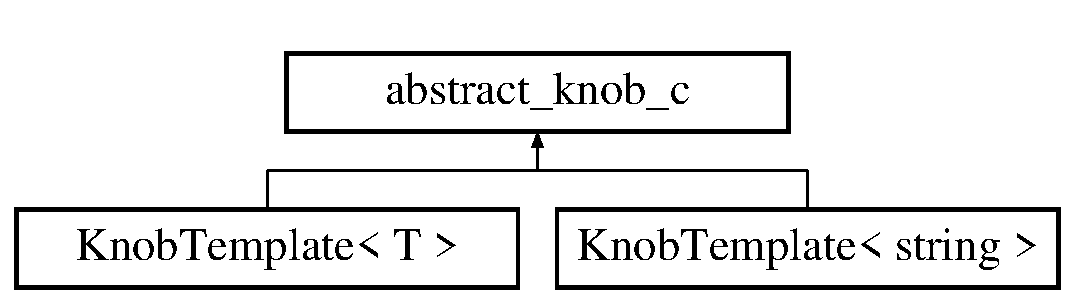
\includegraphics[height=2.000000cm]{classabstract__knob__c}
\end{center}
\end{figure}
\subsection*{Public Member Functions}
\begin{DoxyCompactItemize}
\item 
\hyperlink{classabstract__knob__c_a28a06d1583abf934dbbf7a5a1f7a5914}{abstract\_\-knob\_\-c} ()
\item 
\hyperlink{classabstract__knob__c_acfcc8293c8f93c28012500c56ef2144e}{abstract\_\-knob\_\-c} (string name, string value, string parentName)
\item 
string \hyperlink{classabstract__knob__c_ad1f915ecee7975d85279f7f040b049a7}{getName} () const 
\item 
string \hyperlink{classabstract__knob__c_af5b9c320db0a80508fe435d8e37218b7}{getValueString} () const 
\item 
void \hyperlink{classabstract__knob__c_afe502dfe54a0295aca6352730dcc5dee}{setName} (const string \&name)
\item 
void \hyperlink{classabstract__knob__c_a3dea088397b6ce8baa5f45bfea84fa24}{setValueString} (const string \&value)
\item 
string \hyperlink{classabstract__knob__c_a9a2be7153e2344422ed920bc4c2c86e9}{getParentName} () const 
\item 
virtual void \hyperlink{classabstract__knob__c_ad69620dc8974d5c659c6a7828d460e28}{initFromString} (const string \&strVal)=0
\item 
virtual void \hyperlink{classabstract__knob__c_aaee4499a56d94f1831e7945274dfac8b}{display} (ostream \&os)
\item 
bool \hyperlink{classabstract__knob__c_a052bce404094607be148da67f16051a1}{wasValueProvided} ()
\end{DoxyCompactItemize}
\subsection*{Protected Attributes}
\begin{DoxyCompactItemize}
\item 
string \hyperlink{classabstract__knob__c_a706239ddb3144e45278c2285e129ba84}{m\_\-name}
\item 
string \hyperlink{classabstract__knob__c_a9a877666f9147d4f7cce24a410fb04a2}{m\_\-valueString}
\item 
string \hyperlink{classabstract__knob__c_a35408499c80112fa114354a1fc2e892d}{m\_\-parentName}
\item 
bool \hyperlink{classabstract__knob__c_a80ab5654d985a3f6b0c452575975e257}{m\_\-valueProvided}
\end{DoxyCompactItemize}


\subsection{Detailed Description}
Abstract knob class : base class of all other knobs. 

\subsection{Constructor \& Destructor Documentation}
\hypertarget{classabstract__knob__c_a28a06d1583abf934dbbf7a5a1f7a5914}{
\index{abstract\_\-knob\_\-c@{abstract\_\-knob\_\-c}!abstract\_\-knob\_\-c@{abstract\_\-knob\_\-c}}
\index{abstract\_\-knob\_\-c@{abstract\_\-knob\_\-c}!abstract_knob_c@{abstract\_\-knob\_\-c}}
\subsubsection[{abstract\_\-knob\_\-c}]{\setlength{\rightskip}{0pt plus 5cm}abstract\_\-knob\_\-c::abstract\_\-knob\_\-c (
\begin{DoxyParamCaption}
{}
\end{DoxyParamCaption}
)\hspace{0.3cm}{\ttfamily  \mbox{[}inline\mbox{]}}}}
\label{classabstract__knob__c_a28a06d1583abf934dbbf7a5a1f7a5914}
Constructor. \hypertarget{classabstract__knob__c_acfcc8293c8f93c28012500c56ef2144e}{
\index{abstract\_\-knob\_\-c@{abstract\_\-knob\_\-c}!abstract\_\-knob\_\-c@{abstract\_\-knob\_\-c}}
\index{abstract\_\-knob\_\-c@{abstract\_\-knob\_\-c}!abstract_knob_c@{abstract\_\-knob\_\-c}}
\subsubsection[{abstract\_\-knob\_\-c}]{\setlength{\rightskip}{0pt plus 5cm}abstract\_\-knob\_\-c::abstract\_\-knob\_\-c (
\begin{DoxyParamCaption}
\item[{string}]{ name, }
\item[{string}]{ value, }
\item[{string}]{ parentName}
\end{DoxyParamCaption}
)\hspace{0.3cm}{\ttfamily  \mbox{[}inline\mbox{]}}}}
\label{classabstract__knob__c_acfcc8293c8f93c28012500c56ef2144e}
Constructor. 
\begin{DoxyParams}{Parameters}
\item[{\em name}]knob name \item[{\em value}]initial value \item[{\em parentName}]parent knob (for ratio) \end{DoxyParams}


\subsection{Member Function Documentation}
\hypertarget{classabstract__knob__c_aaee4499a56d94f1831e7945274dfac8b}{
\index{abstract\_\-knob\_\-c@{abstract\_\-knob\_\-c}!display@{display}}
\index{display@{display}!abstract_knob_c@{abstract\_\-knob\_\-c}}
\subsubsection[{display}]{\setlength{\rightskip}{0pt plus 5cm}virtual void abstract\_\-knob\_\-c::display (
\begin{DoxyParamCaption}
\item[{ostream \&}]{ os}
\end{DoxyParamCaption}
)\hspace{0.3cm}{\ttfamily  \mbox{[}inline, virtual\mbox{]}}}}
\label{classabstract__knob__c_aaee4499a56d94f1831e7945274dfac8b}
Print knob name and its value. 

Reimplemented in \hyperlink{classKnobTemplate_af9a940a1d590ad63fdef381388935273}{KnobTemplate$<$ T $>$}, \hyperlink{classKnobTemplate_3_01string_01_4_aee99cda916cd052abaf36957bf6e3a03}{KnobTemplate$<$ string $>$}, \hyperlink{classKnobTemplate_af9a940a1d590ad63fdef381388935273}{KnobTemplate$<$ uns8 $>$}, \hyperlink{classKnobTemplate_af9a940a1d590ad63fdef381388935273}{KnobTemplate$<$ float $>$}, \hyperlink{classKnobTemplate_af9a940a1d590ad63fdef381388935273}{KnobTemplate$<$ uns64 $>$}, \hyperlink{classKnobTemplate_af9a940a1d590ad63fdef381388935273}{KnobTemplate$<$ uns16 $>$}, \hyperlink{classKnobTemplate_af9a940a1d590ad63fdef381388935273}{KnobTemplate$<$ int $>$}, \hyperlink{classKnobTemplate_af9a940a1d590ad63fdef381388935273}{KnobTemplate$<$ uns32 $>$}, \hyperlink{classKnobTemplate_af9a940a1d590ad63fdef381388935273}{KnobTemplate$<$ bool $>$}, and \hyperlink{classKnobTemplate_af9a940a1d590ad63fdef381388935273}{KnobTemplate$<$ uns $>$}.

\hypertarget{classabstract__knob__c_ad1f915ecee7975d85279f7f040b049a7}{
\index{abstract\_\-knob\_\-c@{abstract\_\-knob\_\-c}!getName@{getName}}
\index{getName@{getName}!abstract_knob_c@{abstract\_\-knob\_\-c}}
\subsubsection[{getName}]{\setlength{\rightskip}{0pt plus 5cm}string abstract\_\-knob\_\-c::getName (
\begin{DoxyParamCaption}
{}
\end{DoxyParamCaption}
) const\hspace{0.3cm}{\ttfamily  \mbox{[}inline\mbox{]}}}}
\label{classabstract__knob__c_ad1f915ecee7975d85279f7f040b049a7}
Get knob name. \hypertarget{classabstract__knob__c_a9a2be7153e2344422ed920bc4c2c86e9}{
\index{abstract\_\-knob\_\-c@{abstract\_\-knob\_\-c}!getParentName@{getParentName}}
\index{getParentName@{getParentName}!abstract_knob_c@{abstract\_\-knob\_\-c}}
\subsubsection[{getParentName}]{\setlength{\rightskip}{0pt plus 5cm}string abstract\_\-knob\_\-c::getParentName (
\begin{DoxyParamCaption}
{}
\end{DoxyParamCaption}
) const\hspace{0.3cm}{\ttfamily  \mbox{[}inline\mbox{]}}}}
\label{classabstract__knob__c_a9a2be7153e2344422ed920bc4c2c86e9}
Get the parent knob name. \hypertarget{classabstract__knob__c_af5b9c320db0a80508fe435d8e37218b7}{
\index{abstract\_\-knob\_\-c@{abstract\_\-knob\_\-c}!getValueString@{getValueString}}
\index{getValueString@{getValueString}!abstract_knob_c@{abstract\_\-knob\_\-c}}
\subsubsection[{getValueString}]{\setlength{\rightskip}{0pt plus 5cm}string abstract\_\-knob\_\-c::getValueString (
\begin{DoxyParamCaption}
{}
\end{DoxyParamCaption}
) const\hspace{0.3cm}{\ttfamily  \mbox{[}inline\mbox{]}}}}
\label{classabstract__knob__c_af5b9c320db0a80508fe435d8e37218b7}
Get knob value in string. \hypertarget{classabstract__knob__c_ad69620dc8974d5c659c6a7828d460e28}{
\index{abstract\_\-knob\_\-c@{abstract\_\-knob\_\-c}!initFromString@{initFromString}}
\index{initFromString@{initFromString}!abstract_knob_c@{abstract\_\-knob\_\-c}}
\subsubsection[{initFromString}]{\setlength{\rightskip}{0pt plus 5cm}virtual void abstract\_\-knob\_\-c::initFromString (
\begin{DoxyParamCaption}
\item[{const string \&}]{ strVal}
\end{DoxyParamCaption}
)\hspace{0.3cm}{\ttfamily  \mbox{[}pure virtual\mbox{]}}}}
\label{classabstract__knob__c_ad69620dc8974d5c659c6a7828d460e28}
Init knob from the string. 

Implemented in \hyperlink{classKnobTemplate_a56f3e765c947ac3e63f759d7b3188e42}{KnobTemplate$<$ T $>$}, \hyperlink{classKnobTemplate_3_01string_01_4_ae8fc9c5a7ed9be681b059083338902f7}{KnobTemplate$<$ string $>$}, \hyperlink{classKnobTemplate_a56f3e765c947ac3e63f759d7b3188e42}{KnobTemplate$<$ uns8 $>$}, \hyperlink{classKnobTemplate_a56f3e765c947ac3e63f759d7b3188e42}{KnobTemplate$<$ float $>$}, \hyperlink{classKnobTemplate_a56f3e765c947ac3e63f759d7b3188e42}{KnobTemplate$<$ uns64 $>$}, \hyperlink{classKnobTemplate_a56f3e765c947ac3e63f759d7b3188e42}{KnobTemplate$<$ uns16 $>$}, \hyperlink{classKnobTemplate_a56f3e765c947ac3e63f759d7b3188e42}{KnobTemplate$<$ int $>$}, \hyperlink{classKnobTemplate_a56f3e765c947ac3e63f759d7b3188e42}{KnobTemplate$<$ uns32 $>$}, \hyperlink{classKnobTemplate_a56f3e765c947ac3e63f759d7b3188e42}{KnobTemplate$<$ bool $>$}, and \hyperlink{classKnobTemplate_a56f3e765c947ac3e63f759d7b3188e42}{KnobTemplate$<$ uns $>$}.

\hypertarget{classabstract__knob__c_afe502dfe54a0295aca6352730dcc5dee}{
\index{abstract\_\-knob\_\-c@{abstract\_\-knob\_\-c}!setName@{setName}}
\index{setName@{setName}!abstract_knob_c@{abstract\_\-knob\_\-c}}
\subsubsection[{setName}]{\setlength{\rightskip}{0pt plus 5cm}void abstract\_\-knob\_\-c::setName (
\begin{DoxyParamCaption}
\item[{const string \&}]{ name}
\end{DoxyParamCaption}
)\hspace{0.3cm}{\ttfamily  \mbox{[}inline\mbox{]}}}}
\label{classabstract__knob__c_afe502dfe54a0295aca6352730dcc5dee}
Set the name of the knob. \hypertarget{classabstract__knob__c_a3dea088397b6ce8baa5f45bfea84fa24}{
\index{abstract\_\-knob\_\-c@{abstract\_\-knob\_\-c}!setValueString@{setValueString}}
\index{setValueString@{setValueString}!abstract_knob_c@{abstract\_\-knob\_\-c}}
\subsubsection[{setValueString}]{\setlength{\rightskip}{0pt plus 5cm}void abstract\_\-knob\_\-c::setValueString (
\begin{DoxyParamCaption}
\item[{const string \&}]{ value}
\end{DoxyParamCaption}
)\hspace{0.3cm}{\ttfamily  \mbox{[}inline\mbox{]}}}}
\label{classabstract__knob__c_a3dea088397b6ce8baa5f45bfea84fa24}
Set the value of the knob in string. \hypertarget{classabstract__knob__c_a052bce404094607be148da67f16051a1}{
\index{abstract\_\-knob\_\-c@{abstract\_\-knob\_\-c}!wasValueProvided@{wasValueProvided}}
\index{wasValueProvided@{wasValueProvided}!abstract_knob_c@{abstract\_\-knob\_\-c}}
\subsubsection[{wasValueProvided}]{\setlength{\rightskip}{0pt plus 5cm}bool abstract\_\-knob\_\-c::wasValueProvided (
\begin{DoxyParamCaption}
{}
\end{DoxyParamCaption}
)\hspace{0.3cm}{\ttfamily  \mbox{[}inline\mbox{]}}}}
\label{classabstract__knob__c_a052bce404094607be148da67f16051a1}
Was value provided? 

\subsection{Member Data Documentation}
\hypertarget{classabstract__knob__c_a706239ddb3144e45278c2285e129ba84}{
\index{abstract\_\-knob\_\-c@{abstract\_\-knob\_\-c}!m\_\-name@{m\_\-name}}
\index{m\_\-name@{m\_\-name}!abstract_knob_c@{abstract\_\-knob\_\-c}}
\subsubsection[{m\_\-name}]{\setlength{\rightskip}{0pt plus 5cm}string {\bf abstract\_\-knob\_\-c::m\_\-name}\hspace{0.3cm}{\ttfamily  \mbox{[}protected\mbox{]}}}}
\label{classabstract__knob__c_a706239ddb3144e45278c2285e129ba84}
knob name \hypertarget{classabstract__knob__c_a35408499c80112fa114354a1fc2e892d}{
\index{abstract\_\-knob\_\-c@{abstract\_\-knob\_\-c}!m\_\-parentName@{m\_\-parentName}}
\index{m\_\-parentName@{m\_\-parentName}!abstract_knob_c@{abstract\_\-knob\_\-c}}
\subsubsection[{m\_\-parentName}]{\setlength{\rightskip}{0pt plus 5cm}string {\bf abstract\_\-knob\_\-c::m\_\-parentName}\hspace{0.3cm}{\ttfamily  \mbox{[}protected\mbox{]}}}}
\label{classabstract__knob__c_a35408499c80112fa114354a1fc2e892d}
parent knob name \hypertarget{classabstract__knob__c_a80ab5654d985a3f6b0c452575975e257}{
\index{abstract\_\-knob\_\-c@{abstract\_\-knob\_\-c}!m\_\-valueProvided@{m\_\-valueProvided}}
\index{m\_\-valueProvided@{m\_\-valueProvided}!abstract_knob_c@{abstract\_\-knob\_\-c}}
\subsubsection[{m\_\-valueProvided}]{\setlength{\rightskip}{0pt plus 5cm}bool {\bf abstract\_\-knob\_\-c::m\_\-valueProvided}\hspace{0.3cm}{\ttfamily  \mbox{[}protected\mbox{]}}}}
\label{classabstract__knob__c_a80ab5654d985a3f6b0c452575975e257}
value provided \hypertarget{classabstract__knob__c_a9a877666f9147d4f7cce24a410fb04a2}{
\index{abstract\_\-knob\_\-c@{abstract\_\-knob\_\-c}!m\_\-valueString@{m\_\-valueString}}
\index{m\_\-valueString@{m\_\-valueString}!abstract_knob_c@{abstract\_\-knob\_\-c}}
\subsubsection[{m\_\-valueString}]{\setlength{\rightskip}{0pt plus 5cm}string {\bf abstract\_\-knob\_\-c::m\_\-valueString}\hspace{0.3cm}{\ttfamily  \mbox{[}protected\mbox{]}}}}
\label{classabstract__knob__c_a9a877666f9147d4f7cce24a410fb04a2}
knob value in string 

The documentation for this class was generated from the following file:\begin{DoxyCompactItemize}
\item 
knob.h\end{DoxyCompactItemize}

\hypertarget{classAbstractStat}{
\section{AbstractStat Class Reference}
\label{classAbstractStat}\index{AbstractStat@{AbstractStat}}
}


Statistics base class.  




{\ttfamily \#include $<$statistics.h$>$}

Inheritance diagram for AbstractStat:\begin{figure}[H]
\begin{center}
\leavevmode
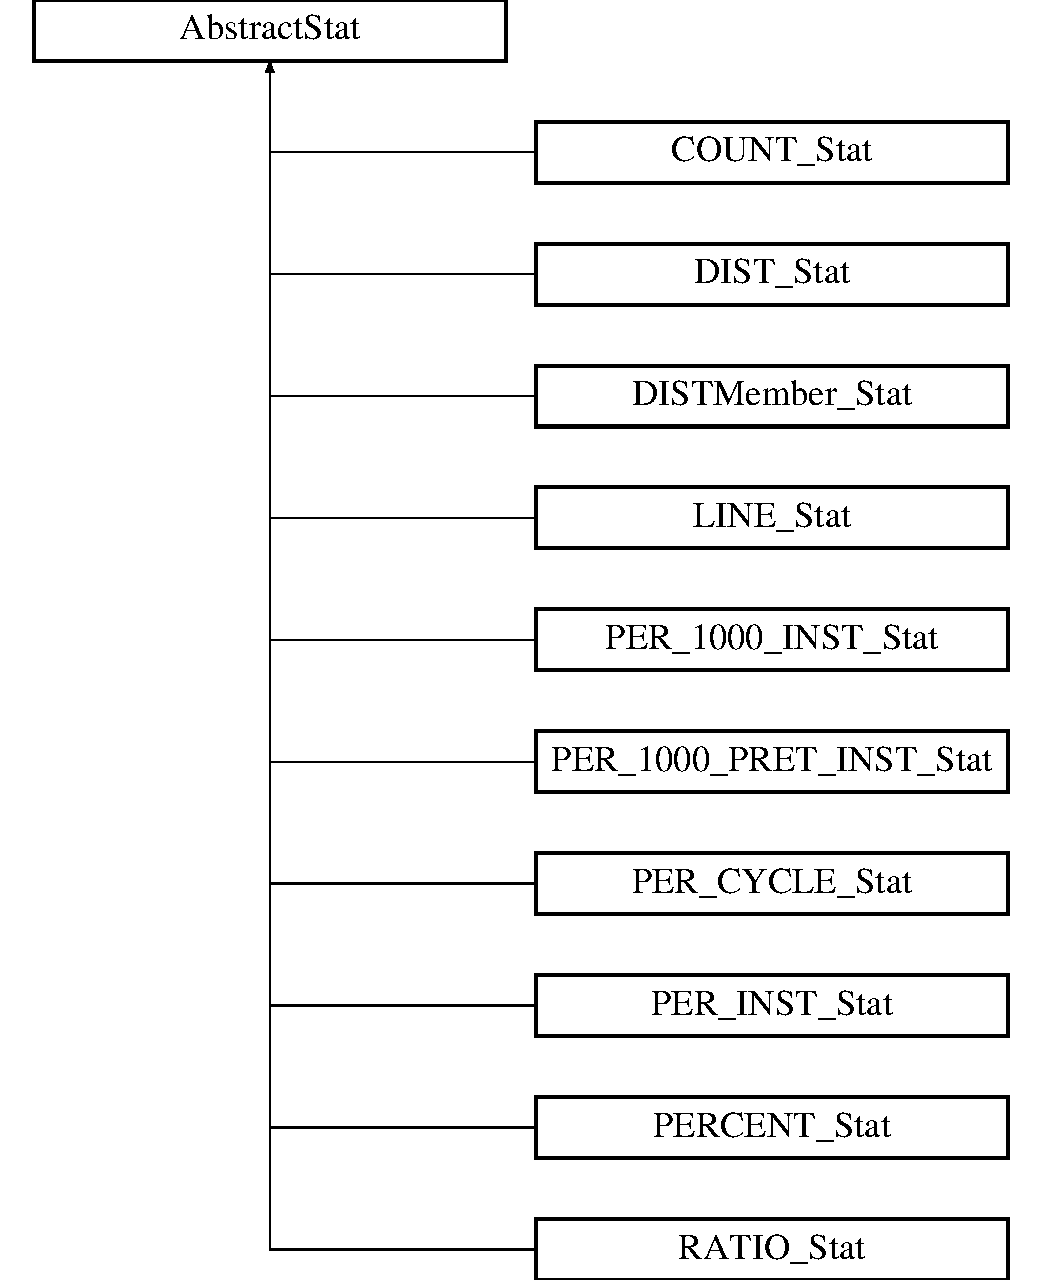
\includegraphics[height=11.000000cm]{classAbstractStat}
\end{center}
\end{figure}
\subsection*{Public Member Functions}
\begin{DoxyCompactItemize}
\item 
\hyperlink{classAbstractStat_a1fefc0acf03b173a655286a1ecb51618}{AbstractStat} (const string \&str, const string \&outputfilename, long ID, bool corewide=false, bool isTemplate=true)
\item 
virtual \hyperlink{classAbstractStat_a68d27fe0b5592399df77bb6e681e8b5e}{$\sim$AbstractStat} ()
\item 
virtual \hyperlink{classAbstractStat}{AbstractStat} $\ast$ \hyperlink{classAbstractStat_aed9a458491d92fb2cc3c458990d9fab1}{clone} (unsigned int coreID)=0
\item 
virtual bool \hyperlink{classAbstractStat_a8b819d1de7dd14edb854545329484506}{memberOfDistribution} ()
\item 
void \hyperlink{classAbstractStat_a4ba3cbe5bcbbf922be0b0b0101c1931c}{setCoreID} (unsigned int coreID)
\item 
const string \& \hyperlink{classAbstractStat_acc7e262331b3d7d15bff6da1656f663c}{getOutputFilename} ()
\item 
const string \& \hyperlink{classAbstractStat_a6a34495d13bcc699bdc93097b9126e1c}{getName} ()
\item 
void \hyperlink{classAbstractStat_a8680b7ffff5ee2ce31f705c62d1c0c17}{inc} ()
\item 
void \hyperlink{classAbstractStat_ad9686be94bf46c5a6b13905de73ae839}{inc} (unsigned int delta)
\item 
void \hyperlink{classAbstractStat_a6f7ce3ecac297732ca764cab841fe5c1}{operator++} (int)
\item 
void \hyperlink{classAbstractStat_a034988d1f13e337dd03a440dbf0220d5}{operator-\/-\/} (int)
\item 
void \hyperlink{classAbstractStat_abda03736dff81db196a3ba5f68bfa59b}{operator+=} (unsigned int delta)
\item 
unsigned long long \hyperlink{classAbstractStat_a90056a981a2a113065d1afb4006e4d00}{getCount} ()
\item 
virtual void \hyperlink{classAbstractStat_aa4760247da47c70d7345de5d881f59cb}{writeTo} (ofstream \&stream)
\end{DoxyCompactItemize}
\subsection*{Protected Attributes}
\begin{DoxyCompactItemize}
\item 
string \hyperlink{classAbstractStat_a0364622ef4333da55eb4ff1ce94444c5}{m\_\-name}
\item 
unsigned long long \hyperlink{classAbstractStat_a01d7f2515084aa821e717b2cb3ecbf34}{m\_\-count}
\item 
unsigned long long \hyperlink{classAbstractStat_a85a84b70539aea2b1318bd45b4d48104}{m\_\-total\_\-count}
\item 
\hyperlink{classAbstractStat}{AbstractStat} $\ast$ \hyperlink{classAbstractStat_a4b62c42003dcc7db965a323a2df01089}{m\_\-pRatioStat}
\item 
string \hyperlink{classAbstractStat_acc58d3d15674660dbf0955193712d36f}{m\_\-fileName}
\item 
long \hyperlink{classAbstractStat_aaa8defb9f5bac0e43ad521ee64334a43}{m\_\-ID}
\item 
bool \hyperlink{classAbstractStat_a39eb3f7796f91946e4fcb76be59c0951}{m\_\-bCoreWide}
\item 
unsigned int \hyperlink{classAbstractStat_ae5f64870f70c46c9d45421298fe14c41}{m\_\-coreID}
\item 
bool \hyperlink{classAbstractStat_aa26aa9ab90712eec3ca55ec236729d9b}{m\_\-isTemplate}
\item 
string \hyperlink{classAbstractStat_af7f98a59844e9417602d28b4849ef105}{m\_\-suffix}
\end{DoxyCompactItemize}
\subsection*{Friends}
\begin{DoxyCompactItemize}
\item 
\hypertarget{classAbstractStat_a4dc9044f574fde5c901b957ff1715ee8}{
class {\bfseries StatisticsDumper}}
\label{classAbstractStat_a4dc9044f574fde5c901b957ff1715ee8}

\end{DoxyCompactItemize}


\subsection{Detailed Description}
Statistics base class. 

\subsection{Constructor \& Destructor Documentation}
\hypertarget{classAbstractStat_a1fefc0acf03b173a655286a1ecb51618}{
\index{AbstractStat@{AbstractStat}!AbstractStat@{AbstractStat}}
\index{AbstractStat@{AbstractStat}!AbstractStat@{AbstractStat}}
\subsubsection[{AbstractStat}]{\setlength{\rightskip}{0pt plus 5cm}AbstractStat::AbstractStat (
\begin{DoxyParamCaption}
\item[{const string \&}]{ str, }
\item[{const string \&}]{ outputfilename, }
\item[{long}]{ ID, }
\item[{bool}]{ corewide = {\ttfamily false}, }
\item[{bool}]{ isTemplate = {\ttfamily true}}
\end{DoxyParamCaption}
)\hspace{0.3cm}{\ttfamily  \mbox{[}inline\mbox{]}}}}
\label{classAbstractStat_a1fefc0acf03b173a655286a1ecb51618}
Constructor. \hypertarget{classAbstractStat_a68d27fe0b5592399df77bb6e681e8b5e}{
\index{AbstractStat@{AbstractStat}!$\sim$AbstractStat@{$\sim$AbstractStat}}
\index{$\sim$AbstractStat@{$\sim$AbstractStat}!AbstractStat@{AbstractStat}}
\subsubsection[{$\sim$AbstractStat}]{\setlength{\rightskip}{0pt plus 5cm}virtual AbstractStat::$\sim$AbstractStat (
\begin{DoxyParamCaption}
{}
\end{DoxyParamCaption}
)\hspace{0.3cm}{\ttfamily  \mbox{[}inline, virtual\mbox{]}}}}
\label{classAbstractStat_a68d27fe0b5592399df77bb6e681e8b5e}
Destructor. 

\subsection{Member Function Documentation}
\hypertarget{classAbstractStat_aed9a458491d92fb2cc3c458990d9fab1}{
\index{AbstractStat@{AbstractStat}!clone@{clone}}
\index{clone@{clone}!AbstractStat@{AbstractStat}}
\subsubsection[{clone}]{\setlength{\rightskip}{0pt plus 5cm}virtual {\bf AbstractStat}$\ast$ AbstractStat::clone (
\begin{DoxyParamCaption}
\item[{unsigned int}]{ coreID}
\end{DoxyParamCaption}
)\hspace{0.3cm}{\ttfamily  \mbox{[}pure virtual\mbox{]}}}}
\label{classAbstractStat_aed9a458491d92fb2cc3c458990d9fab1}
Clone a stat. 

Implemented in \hyperlink{classCOUNT__Stat_ad985ac068e44a565f76f1615b2677022}{COUNT\_\-Stat}, \hyperlink{classDISTMember__Stat_a3a20618868cfc2ac768e0e640049ffad}{DISTMember\_\-Stat}, \hyperlink{classDIST__Stat_a11f5f75a5f6d8551e342a23e72f27809}{DIST\_\-Stat}, \hyperlink{classPER__INST__Stat_a46a249720fb40d3ddef0c2f39c241c03}{PER\_\-INST\_\-Stat}, \hyperlink{classPER__CYCLE__Stat_ae97b00337c422362a6a234b854141bdc}{PER\_\-CYCLE\_\-Stat}, \hyperlink{classRATIO__Stat_af0050320d2f308a6c076992e52c9ad27}{RATIO\_\-Stat}, \hyperlink{classPERCENT__Stat_addd937bd0a1e3649ee2fb6e336ef5955}{PERCENT\_\-Stat}, \hyperlink{classPER__1000__INST__Stat_aa91568b17fd503ba676dd22dfbc13e9a}{PER\_\-1000\_\-INST\_\-Stat}, and \hyperlink{classPER__1000__PRET__INST__Stat_a2aca938ef3f2acc92c46e3386680e5aa}{PER\_\-1000\_\-PRET\_\-INST\_\-Stat}.

\hypertarget{classAbstractStat_a90056a981a2a113065d1afb4006e4d00}{
\index{AbstractStat@{AbstractStat}!getCount@{getCount}}
\index{getCount@{getCount}!AbstractStat@{AbstractStat}}
\subsubsection[{getCount}]{\setlength{\rightskip}{0pt plus 5cm}unsigned long long AbstractStat::getCount (
\begin{DoxyParamCaption}
{}
\end{DoxyParamCaption}
)\hspace{0.3cm}{\ttfamily  \mbox{[}inline\mbox{]}}}}
\label{classAbstractStat_a90056a981a2a113065d1afb4006e4d00}
Get the value of the counter. \hypertarget{classAbstractStat_a6a34495d13bcc699bdc93097b9126e1c}{
\index{AbstractStat@{AbstractStat}!getName@{getName}}
\index{getName@{getName}!AbstractStat@{AbstractStat}}
\subsubsection[{getName}]{\setlength{\rightskip}{0pt plus 5cm}const string\& AbstractStat::getName (
\begin{DoxyParamCaption}
{}
\end{DoxyParamCaption}
)\hspace{0.3cm}{\ttfamily  \mbox{[}inline\mbox{]}}}}
\label{classAbstractStat_a6a34495d13bcc699bdc93097b9126e1c}
Get the name of stat. \hypertarget{classAbstractStat_acc7e262331b3d7d15bff6da1656f663c}{
\index{AbstractStat@{AbstractStat}!getOutputFilename@{getOutputFilename}}
\index{getOutputFilename@{getOutputFilename}!AbstractStat@{AbstractStat}}
\subsubsection[{getOutputFilename}]{\setlength{\rightskip}{0pt plus 5cm}const string\& AbstractStat::getOutputFilename (
\begin{DoxyParamCaption}
{}
\end{DoxyParamCaption}
)\hspace{0.3cm}{\ttfamily  \mbox{[}inline\mbox{]}}}}
\label{classAbstractStat_acc7e262331b3d7d15bff6da1656f663c}
Get output file name. \hypertarget{classAbstractStat_a8680b7ffff5ee2ce31f705c62d1c0c17}{
\index{AbstractStat@{AbstractStat}!inc@{inc}}
\index{inc@{inc}!AbstractStat@{AbstractStat}}
\subsubsection[{inc}]{\setlength{\rightskip}{0pt plus 5cm}void AbstractStat::inc (
\begin{DoxyParamCaption}
{}
\end{DoxyParamCaption}
)\hspace{0.3cm}{\ttfamily  \mbox{[}inline\mbox{]}}}}
\label{classAbstractStat_a8680b7ffff5ee2ce31f705c62d1c0c17}
Increment the counter. \hypertarget{classAbstractStat_ad9686be94bf46c5a6b13905de73ae839}{
\index{AbstractStat@{AbstractStat}!inc@{inc}}
\index{inc@{inc}!AbstractStat@{AbstractStat}}
\subsubsection[{inc}]{\setlength{\rightskip}{0pt plus 5cm}void AbstractStat::inc (
\begin{DoxyParamCaption}
\item[{unsigned int}]{ delta}
\end{DoxyParamCaption}
)\hspace{0.3cm}{\ttfamily  \mbox{[}inline\mbox{]}}}}
\label{classAbstractStat_ad9686be94bf46c5a6b13905de73ae839}
Increase the counter \hypertarget{classAbstractStat_a8b819d1de7dd14edb854545329484506}{
\index{AbstractStat@{AbstractStat}!memberOfDistribution@{memberOfDistribution}}
\index{memberOfDistribution@{memberOfDistribution}!AbstractStat@{AbstractStat}}
\subsubsection[{memberOfDistribution}]{\setlength{\rightskip}{0pt plus 5cm}virtual bool AbstractStat::memberOfDistribution (
\begin{DoxyParamCaption}
{}
\end{DoxyParamCaption}
)\hspace{0.3cm}{\ttfamily  \mbox{[}inline, virtual\mbox{]}}}}
\label{classAbstractStat_a8b819d1de7dd14edb854545329484506}
Not a distribution stat. 

Reimplemented in \hyperlink{classDISTMember__Stat_a0b0238ffd723c62d9f1d52c7499296c0}{DISTMember\_\-Stat}.

\hypertarget{classAbstractStat_a6f7ce3ecac297732ca764cab841fe5c1}{
\index{AbstractStat@{AbstractStat}!operator++@{operator++}}
\index{operator++@{operator++}!AbstractStat@{AbstractStat}}
\subsubsection[{operator++}]{\setlength{\rightskip}{0pt plus 5cm}void AbstractStat::operator++ (
\begin{DoxyParamCaption}
\item[{int}]{}
\end{DoxyParamCaption}
)\hspace{0.3cm}{\ttfamily  \mbox{[}inline\mbox{]}}}}
\label{classAbstractStat_a6f7ce3ecac297732ca764cab841fe5c1}
Operator ++ : increment the counter. \hypertarget{classAbstractStat_abda03736dff81db196a3ba5f68bfa59b}{
\index{AbstractStat@{AbstractStat}!operator+=@{operator+=}}
\index{operator+=@{operator+=}!AbstractStat@{AbstractStat}}
\subsubsection[{operator+=}]{\setlength{\rightskip}{0pt plus 5cm}void AbstractStat::operator+= (
\begin{DoxyParamCaption}
\item[{unsigned int}]{ delta}
\end{DoxyParamCaption}
)\hspace{0.3cm}{\ttfamily  \mbox{[}inline\mbox{]}}}}
\label{classAbstractStat_abda03736dff81db196a3ba5f68bfa59b}
Operator += : increase the counter. \hypertarget{classAbstractStat_a034988d1f13e337dd03a440dbf0220d5}{
\index{AbstractStat@{AbstractStat}!operator-\/-\/@{operator-\/-\/}}
\index{operator-\/-\/@{operator-\/-\/}!AbstractStat@{AbstractStat}}
\subsubsection[{operator-\/-\/}]{\setlength{\rightskip}{0pt plus 5cm}void AbstractStat::operator-\/-\/ (
\begin{DoxyParamCaption}
\item[{int}]{}
\end{DoxyParamCaption}
)\hspace{0.3cm}{\ttfamily  \mbox{[}inline\mbox{]}}}}
\label{classAbstractStat_a034988d1f13e337dd03a440dbf0220d5}
Operator -\/-\/ : decrement the counter. \hypertarget{classAbstractStat_a4ba3cbe5bcbbf922be0b0b0101c1931c}{
\index{AbstractStat@{AbstractStat}!setCoreID@{setCoreID}}
\index{setCoreID@{setCoreID}!AbstractStat@{AbstractStat}}
\subsubsection[{setCoreID}]{\setlength{\rightskip}{0pt plus 5cm}void AbstractStat::setCoreID (
\begin{DoxyParamCaption}
\item[{unsigned int}]{ coreID}
\end{DoxyParamCaption}
)\hspace{0.3cm}{\ttfamily  \mbox{[}inline\mbox{]}}}}
\label{classAbstractStat_a4ba3cbe5bcbbf922be0b0b0101c1931c}
Set the core id. \hypertarget{classAbstractStat_aa4760247da47c70d7345de5d881f59cb}{
\index{AbstractStat@{AbstractStat}!writeTo@{writeTo}}
\index{writeTo@{writeTo}!AbstractStat@{AbstractStat}}
\subsubsection[{writeTo}]{\setlength{\rightskip}{0pt plus 5cm}virtual void AbstractStat::writeTo (
\begin{DoxyParamCaption}
\item[{ofstream \&}]{ stream}
\end{DoxyParamCaption}
)\hspace{0.3cm}{\ttfamily  \mbox{[}inline, virtual\mbox{]}}}}
\label{classAbstractStat_aa4760247da47c70d7345de5d881f59cb}
Dump out all stats to the file. 

Reimplemented in \hyperlink{classDIST__Stat_a521cb2140eba939df71b12dfe805386a}{DIST\_\-Stat}, \hyperlink{classPER__INST__Stat_ad7ffab56cc4bbd33c3332de3863e9b54}{PER\_\-INST\_\-Stat}, \hyperlink{classPER__CYCLE__Stat_afbaf94b274ded7040fe3592a44cc5769}{PER\_\-CYCLE\_\-Stat}, \hyperlink{classRATIO__Stat_a0bf776a3a5dbd304185c2fce9d04934e}{RATIO\_\-Stat}, \hyperlink{classPERCENT__Stat_a927dba3cbaf53d4bc05de92f682f9c80}{PERCENT\_\-Stat}, \hyperlink{classPER__1000__INST__Stat_adb9d735306e7c9a831c92662cfcb8824}{PER\_\-1000\_\-INST\_\-Stat}, and \hyperlink{classPER__1000__PRET__INST__Stat_aa353396e1c813cd55b6023de87abd807}{PER\_\-1000\_\-PRET\_\-INST\_\-Stat}.



\subsection{Member Data Documentation}
\hypertarget{classAbstractStat_a39eb3f7796f91946e4fcb76be59c0951}{
\index{AbstractStat@{AbstractStat}!m\_\-bCoreWide@{m\_\-bCoreWide}}
\index{m\_\-bCoreWide@{m\_\-bCoreWide}!AbstractStat@{AbstractStat}}
\subsubsection[{m\_\-bCoreWide}]{\setlength{\rightskip}{0pt plus 5cm}bool {\bf AbstractStat::m\_\-bCoreWide}\hspace{0.3cm}{\ttfamily  \mbox{[}protected\mbox{]}}}}
\label{classAbstractStat_a39eb3f7796f91946e4fcb76be59c0951}
when set, add suffix to the name of a stat \hypertarget{classAbstractStat_ae5f64870f70c46c9d45421298fe14c41}{
\index{AbstractStat@{AbstractStat}!m\_\-coreID@{m\_\-coreID}}
\index{m\_\-coreID@{m\_\-coreID}!AbstractStat@{AbstractStat}}
\subsubsection[{m\_\-coreID}]{\setlength{\rightskip}{0pt plus 5cm}unsigned int {\bf AbstractStat::m\_\-coreID}\hspace{0.3cm}{\ttfamily  \mbox{[}protected\mbox{]}}}}
\label{classAbstractStat_ae5f64870f70c46c9d45421298fe14c41}
core id \hypertarget{classAbstractStat_a01d7f2515084aa821e717b2cb3ecbf34}{
\index{AbstractStat@{AbstractStat}!m\_\-count@{m\_\-count}}
\index{m\_\-count@{m\_\-count}!AbstractStat@{AbstractStat}}
\subsubsection[{m\_\-count}]{\setlength{\rightskip}{0pt plus 5cm}unsigned long long {\bf AbstractStat::m\_\-count}\hspace{0.3cm}{\ttfamily  \mbox{[}protected\mbox{]}}}}
\label{classAbstractStat_a01d7f2515084aa821e717b2cb3ecbf34}
count during the current stat interval \hypertarget{classAbstractStat_acc58d3d15674660dbf0955193712d36f}{
\index{AbstractStat@{AbstractStat}!m\_\-fileName@{m\_\-fileName}}
\index{m\_\-fileName@{m\_\-fileName}!AbstractStat@{AbstractStat}}
\subsubsection[{m\_\-fileName}]{\setlength{\rightskip}{0pt plus 5cm}string {\bf AbstractStat::m\_\-fileName}\hspace{0.3cm}{\ttfamily  \mbox{[}protected\mbox{]}}}}
\label{classAbstractStat_acc58d3d15674660dbf0955193712d36f}
name of file to print stats \hypertarget{classAbstractStat_aaa8defb9f5bac0e43ad521ee64334a43}{
\index{AbstractStat@{AbstractStat}!m\_\-ID@{m\_\-ID}}
\index{m\_\-ID@{m\_\-ID}!AbstractStat@{AbstractStat}}
\subsubsection[{m\_\-ID}]{\setlength{\rightskip}{0pt plus 5cm}long {\bf AbstractStat::m\_\-ID}\hspace{0.3cm}{\ttfamily  \mbox{[}protected\mbox{]}}}}
\label{classAbstractStat_aaa8defb9f5bac0e43ad521ee64334a43}
stat id \hypertarget{classAbstractStat_aa26aa9ab90712eec3ca55ec236729d9b}{
\index{AbstractStat@{AbstractStat}!m\_\-isTemplate@{m\_\-isTemplate}}
\index{m\_\-isTemplate@{m\_\-isTemplate}!AbstractStat@{AbstractStat}}
\subsubsection[{m\_\-isTemplate}]{\setlength{\rightskip}{0pt plus 5cm}bool {\bf AbstractStat::m\_\-isTemplate}\hspace{0.3cm}{\ttfamily  \mbox{[}protected\mbox{]}}}}
\label{classAbstractStat_aa26aa9ab90712eec3ca55ec236729d9b}
is template \hypertarget{classAbstractStat_a0364622ef4333da55eb4ff1ce94444c5}{
\index{AbstractStat@{AbstractStat}!m\_\-name@{m\_\-name}}
\index{m\_\-name@{m\_\-name}!AbstractStat@{AbstractStat}}
\subsubsection[{m\_\-name}]{\setlength{\rightskip}{0pt plus 5cm}string {\bf AbstractStat::m\_\-name}\hspace{0.3cm}{\ttfamily  \mbox{[}protected\mbox{]}}}}
\label{classAbstractStat_a0364622ef4333da55eb4ff1ce94444c5}
name of stat \hypertarget{classAbstractStat_a4b62c42003dcc7db965a323a2df01089}{
\index{AbstractStat@{AbstractStat}!m\_\-pRatioStat@{m\_\-pRatioStat}}
\index{m\_\-pRatioStat@{m\_\-pRatioStat}!AbstractStat@{AbstractStat}}
\subsubsection[{m\_\-pRatioStat}]{\setlength{\rightskip}{0pt plus 5cm}{\bf AbstractStat}$\ast$ {\bf AbstractStat::m\_\-pRatioStat}\hspace{0.3cm}{\ttfamily  \mbox{[}protected\mbox{]}}}}
\label{classAbstractStat_a4b62c42003dcc7db965a323a2df01089}
stat that to use in the ratio \hypertarget{classAbstractStat_af7f98a59844e9417602d28b4849ef105}{
\index{AbstractStat@{AbstractStat}!m\_\-suffix@{m\_\-suffix}}
\index{m\_\-suffix@{m\_\-suffix}!AbstractStat@{AbstractStat}}
\subsubsection[{m\_\-suffix}]{\setlength{\rightskip}{0pt plus 5cm}string {\bf AbstractStat::m\_\-suffix}\hspace{0.3cm}{\ttfamily  \mbox{[}protected\mbox{]}}}}
\label{classAbstractStat_af7f98a59844e9417602d28b4849ef105}
stat suffix \hypertarget{classAbstractStat_a85a84b70539aea2b1318bd45b4d48104}{
\index{AbstractStat@{AbstractStat}!m\_\-total\_\-count@{m\_\-total\_\-count}}
\index{m\_\-total\_\-count@{m\_\-total\_\-count}!AbstractStat@{AbstractStat}}
\subsubsection[{m\_\-total\_\-count}]{\setlength{\rightskip}{0pt plus 5cm}unsigned long long {\bf AbstractStat::m\_\-total\_\-count}\hspace{0.3cm}{\ttfamily  \mbox{[}protected\mbox{]}}}}
\label{classAbstractStat_a85a84b70539aea2b1318bd45b4d48104}
total count from beginning of run 

The documentation for this class was generated from the following file:\begin{DoxyCompactItemize}
\item 
statistics.h\end{DoxyCompactItemize}

\hypertarget{classall__knobs__c}{
\section{all\_\-knobs\_\-c Class Reference}
\label{classall__knobs__c}\index{all\_\-knobs\_\-c@{all\_\-knobs\_\-c}}
}
\subsection*{Public Member Functions}
\begin{DoxyCompactItemize}
\item 
\hypertarget{classall__knobs__c_a770303b36194353497af9ddc8ef2706f}{
void {\bfseries registerKnobs} (\hyperlink{classKnobsContainer}{KnobsContainer} $\ast$container)}
\label{classall__knobs__c_a770303b36194353497af9ddc8ef2706f}

\end{DoxyCompactItemize}
\subsection*{Public Attributes}
\begin{DoxyCompactItemize}
\item 
\hypertarget{classall__knobs__c_a1f6363ae6857d8f629f9b80868180d87}{
\hyperlink{classKnobTemplate}{KnobTemplate}$<$ uns $>$ $\ast$ {\bfseries KNOB\_\-BP\_\-HIST\_\-LENGTH}}
\label{classall__knobs__c_a1f6363ae6857d8f629f9b80868180d87}

\item 
\hypertarget{classall__knobs__c_a53a1e912a8f695de593f6e7630f13a81}{
\hyperlink{classKnobTemplate}{KnobTemplate}$<$ uns $>$ $\ast$ {\bfseries KNOB\_\-PHT\_\-CTR\_\-BITS}}
\label{classall__knobs__c_a53a1e912a8f695de593f6e7630f13a81}

\item 
\hypertarget{classall__knobs__c_aa7be9696c727c4b2378db21af57b8a99}{
\hyperlink{classKnobTemplate}{KnobTemplate}$<$ string $>$ $\ast$ {\bfseries KNOB\_\-BP\_\-DIR\_\-MECH}}
\label{classall__knobs__c_aa7be9696c727c4b2378db21af57b8a99}

\item 
\hypertarget{classall__knobs__c_ac28c2e0bd4c7e74f11ee4362706a257b}{
\hyperlink{classKnobTemplate}{KnobTemplate}$<$ uns $>$ $\ast$ {\bfseries KNOB\_\-EXTRA\_\-RECOVERY\_\-CYCLES}}
\label{classall__knobs__c_ac28c2e0bd4c7e74f11ee4362706a257b}

\item 
\hypertarget{classall__knobs__c_a447ff7a6346b64d976a8441a4d1f6576}{
\hyperlink{classKnobTemplate}{KnobTemplate}$<$ bool $>$ $\ast$ {\bfseries KNOB\_\-USE\_\-BRANCH\_\-PREDICTION}}
\label{classall__knobs__c_a447ff7a6346b64d976a8441a4d1f6576}

\item 
\hypertarget{classall__knobs__c_aac13686cfde24efc6deeb52a15c7e717}{
\hyperlink{classKnobTemplate}{KnobTemplate}$<$ bool $>$ $\ast$ {\bfseries KNOB\_\-PERFECT\_\-BP}}
\label{classall__knobs__c_aac13686cfde24efc6deeb52a15c7e717}

\item 
\hypertarget{classall__knobs__c_aeb38948c6336978437d7eaf4d61eaba6}{
\hyperlink{classKnobTemplate}{KnobTemplate}$<$ bool $>$ $\ast$ {\bfseries KNOB\_\-PERFECT\_\-BTB}}
\label{classall__knobs__c_aeb38948c6336978437d7eaf4d61eaba6}

\item 
\hypertarget{classall__knobs__c_abddba6c25c84d952f2e2e2175ccad9aa}{
\hyperlink{classKnobTemplate}{KnobTemplate}$<$ uns $>$ $\ast$ {\bfseries KNOB\_\-BTB\_\-ENTRIES}}
\label{classall__knobs__c_abddba6c25c84d952f2e2e2175ccad9aa}

\item 
\hypertarget{classall__knobs__c_abc47b44f5e88a96878f7aee8b0bb1e27}{
\hyperlink{classKnobTemplate}{KnobTemplate}$<$ uns $>$ $\ast$ {\bfseries KNOB\_\-BTB\_\-ASSOC}}
\label{classall__knobs__c_abc47b44f5e88a96878f7aee8b0bb1e27}

\item 
\hypertarget{classall__knobs__c_ab4bac7f71631adafff03e4fea6775f9f}{
\hyperlink{classKnobTemplate}{KnobTemplate}$<$ uns $>$ $\ast$ {\bfseries KNOB\_\-BTB\_\-BANK\_\-NUM}}
\label{classall__knobs__c_ab4bac7f71631adafff03e4fea6775f9f}

\item 
\hypertarget{classall__knobs__c_a0daf0109339ffd89677608933f148b0c}{
\hyperlink{classKnobTemplate}{KnobTemplate}$<$ bool $>$ $\ast$ {\bfseries KNOB\_\-ENABLE\_\-BTB}}
\label{classall__knobs__c_a0daf0109339ffd89677608933f148b0c}

\item 
\hypertarget{classall__knobs__c_acb81c1bbd00f4dc8a6f59f022450fe69}{
\hyperlink{classKnobTemplate}{KnobTemplate}$<$ uns32 $>$ $\ast$ {\bfseries KNOB\_\-FE\_\-SIZE}}
\label{classall__knobs__c_acb81c1bbd00f4dc8a6f59f022450fe69}

\item 
\hypertarget{classall__knobs__c_ad6d1a84a4f79aef5c1969d4961130638}{
\hyperlink{classKnobTemplate}{KnobTemplate}$<$ uns32 $>$ $\ast$ {\bfseries KNOB\_\-SCHED\_\-CLOCK}}
\label{classall__knobs__c_ad6d1a84a4f79aef5c1969d4961130638}

\item 
\hypertarget{classall__knobs__c_a61d6e6d75f62822dee192eaf596a2f85}{
\hyperlink{classKnobTemplate}{KnobTemplate}$<$ uns32 $>$ $\ast$ {\bfseries KNOB\_\-ALLOC\_\-TO\_\-EXEC\_\-LATENCY}}
\label{classall__knobs__c_a61d6e6d75f62822dee192eaf596a2f85}

\item 
\hypertarget{classall__knobs__c_a3d8b224a97f254c9437ead30c34372d5}{
\hyperlink{classKnobTemplate}{KnobTemplate}$<$ uns32 $>$ $\ast$ {\bfseries KNOB\_\-GIAQ\_\-SIZE}}
\label{classall__knobs__c_a3d8b224a97f254c9437ead30c34372d5}

\item 
\hypertarget{classall__knobs__c_a17e5c99b29440ee96048eb519e8fcae6}{
\hyperlink{classKnobTemplate}{KnobTemplate}$<$ uns32 $>$ $\ast$ {\bfseries KNOB\_\-MIAQ\_\-SIZE}}
\label{classall__knobs__c_a17e5c99b29440ee96048eb519e8fcae6}

\item 
\hypertarget{classall__knobs__c_ae131013083248588903b91d1f32a4a77}{
\hyperlink{classKnobTemplate}{KnobTemplate}$<$ uns32 $>$ $\ast$ {\bfseries KNOB\_\-FQ\_\-SIZE}}
\label{classall__knobs__c_ae131013083248588903b91d1f32a4a77}

\item 
\hypertarget{classall__knobs__c_a0e6368a53d862dc2fa52038df9173d7e}{
\hyperlink{classKnobTemplate}{KnobTemplate}$<$ uns32 $>$ $\ast$ {\bfseries KNOB\_\-GIAQ\_\-MEDIUM\_\-SIZE}}
\label{classall__knobs__c_a0e6368a53d862dc2fa52038df9173d7e}

\item 
\hypertarget{classall__knobs__c_a8fb7846e838b7a45b03215d114d86342}{
\hyperlink{classKnobTemplate}{KnobTemplate}$<$ uns32 $>$ $\ast$ {\bfseries KNOB\_\-MIAQ\_\-MEDIUM\_\-SIZE}}
\label{classall__knobs__c_a8fb7846e838b7a45b03215d114d86342}

\item 
\hypertarget{classall__knobs__c_a145e6cfb8f599305d9098c732e313282}{
\hyperlink{classKnobTemplate}{KnobTemplate}$<$ uns32 $>$ $\ast$ {\bfseries KNOB\_\-FQ\_\-MEDIUM\_\-SIZE}}
\label{classall__knobs__c_a145e6cfb8f599305d9098c732e313282}

\item 
\hypertarget{classall__knobs__c_adae886ac220a51b8d2b3b49e12ca0251}{
\hyperlink{classKnobTemplate}{KnobTemplate}$<$ uns32 $>$ $\ast$ {\bfseries KNOB\_\-GIAQ\_\-LARGE\_\-SIZE}}
\label{classall__knobs__c_adae886ac220a51b8d2b3b49e12ca0251}

\item 
\hypertarget{classall__knobs__c_a06f387d83d575fbd9afc33fc7b373363}{
\hyperlink{classKnobTemplate}{KnobTemplate}$<$ uns32 $>$ $\ast$ {\bfseries KNOB\_\-MIAQ\_\-LARGE\_\-SIZE}}
\label{classall__knobs__c_a06f387d83d575fbd9afc33fc7b373363}

\item 
\hypertarget{classall__knobs__c_a90de3db4cf191362e868ab3da1ab24a5}{
\hyperlink{classKnobTemplate}{KnobTemplate}$<$ uns32 $>$ $\ast$ {\bfseries KNOB\_\-FQ\_\-LARGE\_\-SIZE}}
\label{classall__knobs__c_a90de3db4cf191362e868ab3da1ab24a5}

\item 
\hypertarget{classall__knobs__c_a4b2e8e685a55e75c49eca227e825dea9}{
\hyperlink{classKnobTemplate}{KnobTemplate}$<$ int $>$ $\ast$ {\bfseries KNOB\_\-GEN\_\-ALLOCQ\_\-INDEX}}
\label{classall__knobs__c_a4b2e8e685a55e75c49eca227e825dea9}

\item 
\hypertarget{classall__knobs__c_a938f4b2aae4e897b4dde949f0c1c2e30}{
\hyperlink{classKnobTemplate}{KnobTemplate}$<$ int $>$ $\ast$ {\bfseries KNOB\_\-MEM\_\-ALLOCQ\_\-INDEX}}
\label{classall__knobs__c_a938f4b2aae4e897b4dde949f0c1c2e30}

\item 
\hypertarget{classall__knobs__c_a0ec215d7422bade9f0b25419ed8c6181}{
\hyperlink{classKnobTemplate}{KnobTemplate}$<$ int $>$ $\ast$ {\bfseries KNOB\_\-FLOAT\_\-ALLOCQ\_\-INDEX}}
\label{classall__knobs__c_a0ec215d7422bade9f0b25419ed8c6181}

\item 
\hypertarget{classall__knobs__c_a2c144aafeb5c53b7efe0b45285f282fb}{
\hyperlink{classKnobTemplate}{KnobTemplate}$<$ bool $>$ $\ast$ {\bfseries KNOB\_\-ONE\_\-CYCLE\_\-EXEC}}
\label{classall__knobs__c_a2c144aafeb5c53b7efe0b45285f282fb}

\item 
\hypertarget{classall__knobs__c_ab1e9660bb6b8b2c50159fead1177864d}{
\hyperlink{classKnobTemplate}{KnobTemplate}$<$ uns32 $>$ $\ast$ {\bfseries KNOB\_\-MAX\_\-INSTS}}
\label{classall__knobs__c_ab1e9660bb6b8b2c50159fead1177864d}

\item 
\hypertarget{classall__knobs__c_ae32ff1c2ebf42f91192e55bb9bec3bce}{
\hyperlink{classKnobTemplate}{KnobTemplate}$<$ uns32 $>$ $\ast$ {\bfseries KNOB\_\-SIM\_\-CYCLE\_\-COUNT}}
\label{classall__knobs__c_ae32ff1c2ebf42f91192e55bb9bec3bce}

\item 
\hypertarget{classall__knobs__c_ad1fcd292f0aa35e35d46e10962b56d2d}{
\hyperlink{classKnobTemplate}{KnobTemplate}$<$ uns64 $>$ $\ast$ {\bfseries KNOB\_\-FORWARD\_\-PROGRESS\_\-LIMIT}}
\label{classall__knobs__c_ad1fcd292f0aa35e35d46e10962b56d2d}

\item 
\hypertarget{classall__knobs__c_a4c19f37418e3b1f995b282b400f59130}{
\hyperlink{classKnobTemplate}{KnobTemplate}$<$ int $>$ $\ast$ {\bfseries KNOB\_\-MAX\_\-BLOCK\_\-PER\_\-CORE\_\-SUPER}}
\label{classall__knobs__c_a4c19f37418e3b1f995b282b400f59130}

\item 
\hypertarget{classall__knobs__c_a92311a2438bb16ccfdfd04f87a5a4ea2}{
\hyperlink{classKnobTemplate}{KnobTemplate}$<$ uns16 $>$ $\ast$ {\bfseries KNOB\_\-ROB\_\-SIZE}}
\label{classall__knobs__c_a92311a2438bb16ccfdfd04f87a5a4ea2}

\item 
\hypertarget{classall__knobs__c_a8866be3f0d7c4428cb51839a7752479e}{
\hyperlink{classKnobTemplate}{KnobTemplate}$<$ uns16 $>$ $\ast$ {\bfseries KNOB\_\-ROB\_\-MEDIUM\_\-SIZE}}
\label{classall__knobs__c_a8866be3f0d7c4428cb51839a7752479e}

\item 
\hypertarget{classall__knobs__c_af97b76d630902a1a4322336a33a17cc7}{
\hyperlink{classKnobTemplate}{KnobTemplate}$<$ uns16 $>$ $\ast$ {\bfseries KNOB\_\-ROB\_\-LARGE\_\-SIZE}}
\label{classall__knobs__c_af97b76d630902a1a4322336a33a17cc7}

\item 
\hypertarget{classall__knobs__c_ae9f995b8aa23028f796ca4ced808b5a3}{
\hyperlink{classKnobTemplate}{KnobTemplate}$<$ uns16 $>$ $\ast$ {\bfseries KNOB\_\-INT\_\-REGFILE\_\-SIZE}}
\label{classall__knobs__c_ae9f995b8aa23028f796ca4ced808b5a3}

\item 
\hypertarget{classall__knobs__c_a10b7b498ac993667a27c417fc7bd35a9}{
\hyperlink{classKnobTemplate}{KnobTemplate}$<$ uns16 $>$ $\ast$ {\bfseries KNOB\_\-FP\_\-REGFILE\_\-SIZE}}
\label{classall__knobs__c_a10b7b498ac993667a27c417fc7bd35a9}

\item 
\hypertarget{classall__knobs__c_a6ac7bb37dd70fff5080a0d0b5ec6dbb3}{
\hyperlink{classKnobTemplate}{KnobTemplate}$<$ uns16 $>$ $\ast$ {\bfseries KNOB\_\-MEU\_\-NSB}}
\label{classall__knobs__c_a6ac7bb37dd70fff5080a0d0b5ec6dbb3}

\item 
\hypertarget{classall__knobs__c_af7be1dfdbc88e19bbff45afaa3c1501a}{
\hyperlink{classKnobTemplate}{KnobTemplate}$<$ uns16 $>$ $\ast$ {\bfseries KNOB\_\-MEU\_\-NLB}}
\label{classall__knobs__c_af7be1dfdbc88e19bbff45afaa3c1501a}

\item 
\hypertarget{classall__knobs__c_af7d70bdfa1b06c656e93757d20aa356c}{
\hyperlink{classKnobTemplate}{KnobTemplate}$<$ uns16 $>$ $\ast$ {\bfseries KNOB\_\-MEU\_\-MEDIUM\_\-NSB}}
\label{classall__knobs__c_af7d70bdfa1b06c656e93757d20aa356c}

\item 
\hypertarget{classall__knobs__c_a03567d9504d4cde8b585afe5b2814410}{
\hyperlink{classKnobTemplate}{KnobTemplate}$<$ uns16 $>$ $\ast$ {\bfseries KNOB\_\-MEU\_\-MEDIUM\_\-NLB}}
\label{classall__knobs__c_a03567d9504d4cde8b585afe5b2814410}

\item 
\hypertarget{classall__knobs__c_a7ba927486d8125c44c4e37d9437ca2b3}{
\hyperlink{classKnobTemplate}{KnobTemplate}$<$ uns16 $>$ $\ast$ {\bfseries KNOB\_\-MEU\_\-LARGE\_\-NSB}}
\label{classall__knobs__c_a7ba927486d8125c44c4e37d9437ca2b3}

\item 
\hypertarget{classall__knobs__c_a6f515d805cb01ae73160b890245b9019}{
\hyperlink{classKnobTemplate}{KnobTemplate}$<$ uns16 $>$ $\ast$ {\bfseries KNOB\_\-MEU\_\-LARGE\_\-NLB}}
\label{classall__knobs__c_a6f515d805cb01ae73160b890245b9019}

\item 
\hypertarget{classall__knobs__c_acb9a88b5a87d929d48ed0066f63f810b}{
\hyperlink{classKnobTemplate}{KnobTemplate}$<$ uns16 $>$ $\ast$ {\bfseries KNOB\_\-WIDTH}}
\label{classall__knobs__c_acb9a88b5a87d929d48ed0066f63f810b}

\item 
\hypertarget{classall__knobs__c_a78b0bd532ebf98729cff646432beb545}{
\hyperlink{classKnobTemplate}{KnobTemplate}$<$ uns16 $>$ $\ast$ {\bfseries KNOB\_\-MEDIUM\_\-WIDTH}}
\label{classall__knobs__c_a78b0bd532ebf98729cff646432beb545}

\item 
\hypertarget{classall__knobs__c_ae344edfc95b1215e15103f411e6db31a}{
\hyperlink{classKnobTemplate}{KnobTemplate}$<$ uns16 $>$ $\ast$ {\bfseries KNOB\_\-LARGE\_\-WIDTH}}
\label{classall__knobs__c_ae344edfc95b1215e15103f411e6db31a}

\item 
\hypertarget{classall__knobs__c_a568caa14adeaebb18ecd02026eb4a369}{
\hyperlink{classKnobTemplate}{KnobTemplate}$<$ int $>$ $\ast$ {\bfseries KNOB\_\-EXEC\_\-RETIRE\_\-LATENCY}}
\label{classall__knobs__c_a568caa14adeaebb18ecd02026eb4a369}

\item 
\hypertarget{classall__knobs__c_afc2421a5abd54aec28fdf68b43a273a0}{
\hyperlink{classKnobTemplate}{KnobTemplate}$<$ bool $>$ $\ast$ {\bfseries KNOB\_\-MEM\_\-OBEY\_\-STORE\_\-DEP}}
\label{classall__knobs__c_afc2421a5abd54aec28fdf68b43a273a0}

\item 
\hypertarget{classall__knobs__c_a7a533ef1bc4e0aee27ebbbc02f2c6e69}{
\hyperlink{classKnobTemplate}{KnobTemplate}$<$ bool $>$ $\ast$ {\bfseries KNOB\_\-MEM\_\-OOO\_\-STORES}}
\label{classall__knobs__c_a7a533ef1bc4e0aee27ebbbc02f2c6e69}

\item 
\hypertarget{classall__knobs__c_ab831e1adc87c3f7f7c4688f65117a48a}{
\hyperlink{classKnobTemplate}{KnobTemplate}$<$ bool $>$ $\ast$ {\bfseries KNOB\_\-USE\_\-NEW\_\-ORACLE}}
\label{classall__knobs__c_ab831e1adc87c3f7f7c4688f65117a48a}

\item 
\hypertarget{classall__knobs__c_adec0427fede9c9b24abff4fa96981beb}{
\hyperlink{classKnobTemplate}{KnobTemplate}$<$ bool $>$ $\ast$ {\bfseries KNOB\_\-IGNORE\_\-DEP}}
\label{classall__knobs__c_adec0427fede9c9b24abff4fa96981beb}

\item 
\hypertarget{classall__knobs__c_aafdcb1db6973b545603053bcbdb813f9}{
\hyperlink{classKnobTemplate}{KnobTemplate}$<$ uns $>$ $\ast$ {\bfseries KNOB\_\-HEARTBEAT\_\-INTERVAL}}
\label{classall__knobs__c_aafdcb1db6973b545603053bcbdb813f9}

\item 
\hypertarget{classall__knobs__c_abc17e99440216e92dd6cd51b5c7c6cfd}{
\hyperlink{classKnobTemplate}{KnobTemplate}$<$ int $>$ $\ast$ {\bfseries KNOB\_\-GPU\_\-FETCH\_\-RATIO}}
\label{classall__knobs__c_abc17e99440216e92dd6cd51b5c7c6cfd}

\item 
\hypertarget{classall__knobs__c_ab401bab322a64300c86aef037c1cf666}{
\hyperlink{classKnobTemplate}{KnobTemplate}$<$ int $>$ $\ast$ {\bfseries KNOB\_\-GPU\_\-SCHEDULE\_\-RATIO}}
\label{classall__knobs__c_ab401bab322a64300c86aef037c1cf666}

\item 
\hypertarget{classall__knobs__c_a05e9bdca383b8c661d1c4aaafed1140e}{
\hyperlink{classKnobTemplate}{KnobTemplate}$<$ int $>$ $\ast$ {\bfseries KNOB\_\-PTX\_\-EXEC\_\-RATIO}}
\label{classall__knobs__c_a05e9bdca383b8c661d1c4aaafed1140e}

\item 
\hypertarget{classall__knobs__c_a523c7f215f2eb58b4c94dff7502773cc}{
\hyperlink{classKnobTemplate}{KnobTemplate}$<$ uns32 $>$ $\ast$ {\bfseries KNOB\_\-NUM\_\-SIM\_\-CORES}}
\label{classall__knobs__c_a523c7f215f2eb58b4c94dff7502773cc}

\item 
\hypertarget{classall__knobs__c_a9c01aec9e1b5f464777ba23cee578e86}{
\hyperlink{classKnobTemplate}{KnobTemplate}$<$ string $>$ $\ast$ {\bfseries KNOB\_\-CORE\_\-TYPE}}
\label{classall__knobs__c_a9c01aec9e1b5f464777ba23cee578e86}

\item 
\hypertarget{classall__knobs__c_a012dbc91f9190969e0a23156f07f13aa}{
\hyperlink{classKnobTemplate}{KnobTemplate}$<$ string $>$ $\ast$ {\bfseries KNOB\_\-MEDIUM\_\-CORE\_\-TYPE}}
\label{classall__knobs__c_a012dbc91f9190969e0a23156f07f13aa}

\item 
\hypertarget{classall__knobs__c_af6c50aca4c8636d13e88f5fbd662d5af}{
\hyperlink{classKnobTemplate}{KnobTemplate}$<$ string $>$ $\ast$ {\bfseries KNOB\_\-LARGE\_\-CORE\_\-TYPE}}
\label{classall__knobs__c_af6c50aca4c8636d13e88f5fbd662d5af}

\item 
\hypertarget{classall__knobs__c_aca875520e9536f6a951f3426f4ed823d}{
\hyperlink{classKnobTemplate}{KnobTemplate}$<$ uns32 $>$ $\ast$ {\bfseries KNOB\_\-NUM\_\-SIM\_\-SMALL\_\-CORES}}
\label{classall__knobs__c_aca875520e9536f6a951f3426f4ed823d}

\item 
\hypertarget{classall__knobs__c_ad54048adcc75d9526d2121cbe4f4cdc2}{
\hyperlink{classKnobTemplate}{KnobTemplate}$<$ uns32 $>$ $\ast$ {\bfseries KNOB\_\-NUM\_\-SIM\_\-LARGE\_\-CORES}}
\label{classall__knobs__c_ad54048adcc75d9526d2121cbe4f4cdc2}

\item 
\hypertarget{classall__knobs__c_ae0b022b66534742da6bfa3467f03f994}{
\hyperlink{classKnobTemplate}{KnobTemplate}$<$ uns32 $>$ $\ast$ {\bfseries KNOB\_\-NUM\_\-SIM\_\-MEDIUM\_\-CORES}}
\label{classall__knobs__c_ae0b022b66534742da6bfa3467f03f994}

\item 
\hypertarget{classall__knobs__c_a6996c338acb7e515e5b118a5b595052b}{
\hyperlink{classKnobTemplate}{KnobTemplate}$<$ int $>$ $\ast$ {\bfseries KNOB\_\-MAX\_\-THREADS\_\-PER\_\-CORE}}
\label{classall__knobs__c_a6996c338acb7e515e5b118a5b595052b}

\item 
\hypertarget{classall__knobs__c_ad8bcb2b478968f68db41a4b2bbd75b03}{
\hyperlink{classKnobTemplate}{KnobTemplate}$<$ int $>$ $\ast$ {\bfseries KNOB\_\-MAX\_\-THREADS\_\-PER\_\-MEDIUM\_\-CORE}}
\label{classall__knobs__c_ad8bcb2b478968f68db41a4b2bbd75b03}

\item 
\hypertarget{classall__knobs__c_a1ba7e5350d7fac6acbacf0d81dfdad30}{
\hyperlink{classKnobTemplate}{KnobTemplate}$<$ int $>$ $\ast$ {\bfseries KNOB\_\-MAX\_\-THREADS\_\-PER\_\-LARGE\_\-CORE}}
\label{classall__knobs__c_a1ba7e5350d7fac6acbacf0d81dfdad30}

\item 
\hypertarget{classall__knobs__c_a73f27be1e4e2a2a14a2699d0429b3652}{
\hyperlink{classKnobTemplate}{KnobTemplate}$<$ string $>$ $\ast$ {\bfseries KNOB\_\-SCHEDULE}}
\label{classall__knobs__c_a73f27be1e4e2a2a14a2699d0429b3652}

\item 
\hypertarget{classall__knobs__c_aa9790c99eb4fc023a8165b9d88f3e554}{
\hyperlink{classKnobTemplate}{KnobTemplate}$<$ string $>$ $\ast$ {\bfseries KNOB\_\-MEDIUM\_\-CORE\_\-SCHEDULE}}
\label{classall__knobs__c_aa9790c99eb4fc023a8165b9d88f3e554}

\item 
\hypertarget{classall__knobs__c_a6fed20719605d044aa969f62e07771a9}{
\hyperlink{classKnobTemplate}{KnobTemplate}$<$ string $>$ $\ast$ {\bfseries KNOB\_\-LARGE\_\-CORE\_\-SCHEDULE}}
\label{classall__knobs__c_a6fed20719605d044aa969f62e07771a9}

\item 
\hypertarget{classall__knobs__c_a45797b033ee995c8cada75c1fa4679eb}{
\hyperlink{classKnobTemplate}{KnobTemplate}$<$ uns32 $>$ $\ast$ {\bfseries KNOB\_\-FETCH\_\-LATENCY}}
\label{classall__knobs__c_a45797b033ee995c8cada75c1fa4679eb}

\item 
\hypertarget{classall__knobs__c_a7e1c4010d12717ea250548055ed79224}{
\hyperlink{classKnobTemplate}{KnobTemplate}$<$ uns32 $>$ $\ast$ {\bfseries KNOB\_\-ALLOC\_\-LATENCY}}
\label{classall__knobs__c_a7e1c4010d12717ea250548055ed79224}

\item 
\hypertarget{classall__knobs__c_a359cc29d7f55c97bdc799bb09130a992}{
\hyperlink{classKnobTemplate}{KnobTemplate}$<$ uns32 $>$ $\ast$ {\bfseries KNOB\_\-MEDIUM\_\-CORE\_\-ALLOC\_\-LATENCY}}
\label{classall__knobs__c_a359cc29d7f55c97bdc799bb09130a992}

\item 
\hypertarget{classall__knobs__c_abbf3f292031a1092d28a7925078fea9e}{
\hyperlink{classKnobTemplate}{KnobTemplate}$<$ uns32 $>$ $\ast$ {\bfseries KNOB\_\-MEDIUM\_\-CORE\_\-FETCH\_\-LATENCY}}
\label{classall__knobs__c_abbf3f292031a1092d28a7925078fea9e}

\item 
\hypertarget{classall__knobs__c_a7fa78d42e21da8818c4baf518e43a6af}{
\hyperlink{classKnobTemplate}{KnobTemplate}$<$ uns32 $>$ $\ast$ {\bfseries KNOB\_\-LARGE\_\-CORE\_\-ALLOC\_\-LATENCY}}
\label{classall__knobs__c_a7fa78d42e21da8818c4baf518e43a6af}

\item 
\hypertarget{classall__knobs__c_a3a328b57d6862c69d6ca6b476ab3ad80}{
\hyperlink{classKnobTemplate}{KnobTemplate}$<$ uns32 $>$ $\ast$ {\bfseries KNOB\_\-LARGE\_\-CORE\_\-FETCH\_\-LATENCY}}
\label{classall__knobs__c_a3a328b57d6862c69d6ca6b476ab3ad80}

\item 
\hypertarget{classall__knobs__c_a9c676a5585857c4cdde93bc83bff302c}{
\hyperlink{classKnobTemplate}{KnobTemplate}$<$ bool $>$ $\ast$ {\bfseries KNOB\_\-PRINT\_\-HEARTBEAT}}
\label{classall__knobs__c_a9c676a5585857c4cdde93bc83bff302c}

\item 
\hypertarget{classall__knobs__c_a8932ac814dca5dccbb4be4d569776d3f}{
\hyperlink{classKnobTemplate}{KnobTemplate}$<$ bool $>$ $\ast$ {\bfseries KNOB\_\-GPU\_\-SCHED}}
\label{classall__knobs__c_a8932ac814dca5dccbb4be4d569776d3f}

\item 
\hypertarget{classall__knobs__c_af4565ded46d7861457aa447e703703b1}{
\hyperlink{classKnobTemplate}{KnobTemplate}$<$ bool $>$ $\ast$ {\bfseries KNOB\_\-GPU\_\-USE\_\-SINGLE\_\-ALLOCQ\_\-TYPE}}
\label{classall__knobs__c_af4565ded46d7861457aa447e703703b1}

\item 
\hypertarget{classall__knobs__c_a421f9130305ec9d9b7a47ca881349a45}{
\hyperlink{classKnobTemplate}{KnobTemplate}$<$ bool $>$ $\ast$ {\bfseries KNOB\_\-GPU\_\-SHARE\_\-ALLOCQS\_\-BETWEEN\_\-THREADS}}
\label{classall__knobs__c_a421f9130305ec9d9b7a47ca881349a45}

\item 
\hypertarget{classall__knobs__c_a0bd21d87b8004f55f3a425a999a60f3b}{
\hyperlink{classKnobTemplate}{KnobTemplate}$<$ int $>$ $\ast$ {\bfseries KNOB\_\-32\_\-64\_\-ISA}}
\label{classall__knobs__c_a0bd21d87b8004f55f3a425a999a60f3b}

\item 
\hypertarget{classall__knobs__c_ab9ab850300de68dfbbbfbe1ed9827560}{
\hyperlink{classKnobTemplate}{KnobTemplate}$<$ int $>$ $\ast$ {\bfseries KNOB\_\-PHY\_\-ADDR\_\-WIDTH}}
\label{classall__knobs__c_ab9ab850300de68dfbbbfbe1ed9827560}

\item 
\hypertarget{classall__knobs__c_a373e0dbc24d6eb41570f833fc9d26528}{
\hyperlink{classKnobTemplate}{KnobTemplate}$<$ int $>$ $\ast$ {\bfseries KNOB\_\-FEATURE\_\-SIZE}}
\label{classall__knobs__c_a373e0dbc24d6eb41570f833fc9d26528}

\item 
\hypertarget{classall__knobs__c_aee6870710693c108d71bef0239660b08}{
\hyperlink{classKnobTemplate}{KnobTemplate}$<$ int $>$ $\ast$ {\bfseries KNOB\_\-PCIE\_\-BUS\_\-SIZE}}
\label{classall__knobs__c_aee6870710693c108d71bef0239660b08}

\item 
\hypertarget{classall__knobs__c_af2eda7cfeb6368d77efb3c7c9f59269a}{
\hyperlink{classKnobTemplate}{KnobTemplate}$<$ int $>$ $\ast$ {\bfseries KNOB\_\-PCIE\_\-TR}}
\label{classall__knobs__c_af2eda7cfeb6368d77efb3c7c9f59269a}

\item 
\hypertarget{classall__knobs__c_abf9d10c8460205ef536cd8f6663fdaad}{
\hyperlink{classKnobTemplate}{KnobTemplate}$<$ int $>$ $\ast$ {\bfseries KNOB\_\-PCIE\_\-INIT}}
\label{classall__knobs__c_abf9d10c8460205ef536cd8f6663fdaad}

\item 
\hypertarget{classall__knobs__c_a09fe5493b3f997b9795e6387744ec20b}{
\hyperlink{classKnobTemplate}{KnobTemplate}$<$ int $>$ $\ast$ {\bfseries KNOB\_\-HOMOGENEOUS\_\-CCS}}
\label{classall__knobs__c_a09fe5493b3f997b9795e6387744ec20b}

\item 
\hypertarget{classall__knobs__c_a5388b0c6d7ef8256f4b22313f9d70750}{
\hyperlink{classKnobTemplate}{KnobTemplate}$<$ int $>$ $\ast$ {\bfseries KNOB\_\-INST\_\-LENGTH}}
\label{classall__knobs__c_a5388b0c6d7ef8256f4b22313f9d70750}

\item 
\hypertarget{classall__knobs__c_a6714c4ef3291f6b553c1c0cc29f075e2}{
\hyperlink{classKnobTemplate}{KnobTemplate}$<$ int $>$ $\ast$ {\bfseries KNOB\_\-OPCODE\_\-WIDTH}}
\label{classall__knobs__c_a6714c4ef3291f6b553c1c0cc29f075e2}

\item 
\hypertarget{classall__knobs__c_a8a8c591ad7890f468b8d43edceef25ee}{
\hyperlink{classKnobTemplate}{KnobTemplate}$<$ int $>$ $\ast$ {\bfseries KNOB\_\-MICRO\_\-OPCODE\_\-WIDTH}}
\label{classall__knobs__c_a8a8c591ad7890f468b8d43edceef25ee}

\item 
\hypertarget{classall__knobs__c_ad39d25dc3a9755c99a987ac22a218429}{
\hyperlink{classKnobTemplate}{KnobTemplate}$<$ int $>$ $\ast$ {\bfseries KNOB\_\-PIPELINE\_\-DEPTH\_\-INT}}
\label{classall__knobs__c_ad39d25dc3a9755c99a987ac22a218429}

\item 
\hypertarget{classall__knobs__c_ab47f180ec7e9b016ce6a497d873b2435}{
\hyperlink{classKnobTemplate}{KnobTemplate}$<$ int $>$ $\ast$ {\bfseries KNOB\_\-PIPELINE\_\-DEPTH\_\-FP}}
\label{classall__knobs__c_ab47f180ec7e9b016ce6a497d873b2435}

\item 
\hypertarget{classall__knobs__c_afe451b702e02e0b21a9febe86b635825}{
\hyperlink{classKnobTemplate}{KnobTemplate}$<$ int $>$ $\ast$ {\bfseries KNOB\_\-ALU\_\-PER\_\-CORE}}
\label{classall__knobs__c_afe451b702e02e0b21a9febe86b635825}

\item 
\hypertarget{classall__knobs__c_a070238fa9851650ceb7c1e05526339af}{
\hyperlink{classKnobTemplate}{KnobTemplate}$<$ int $>$ $\ast$ {\bfseries KNOB\_\-MUL\_\-PER\_\-CORE}}
\label{classall__knobs__c_a070238fa9851650ceb7c1e05526339af}

\item 
\hypertarget{classall__knobs__c_ac148e7ac15a1b9e897b5e166b321d4b5}{
\hyperlink{classKnobTemplate}{KnobTemplate}$<$ int $>$ $\ast$ {\bfseries KNOB\_\-FPU\_\-PER\_\-CORE}}
\label{classall__knobs__c_ac148e7ac15a1b9e897b5e166b321d4b5}

\item 
\hypertarget{classall__knobs__c_af3292053caeec81589754f947ae6ab38}{
\hyperlink{classKnobTemplate}{KnobTemplate}$<$ int $>$ $\ast$ {\bfseries KNOB\_\-INST\_\-BUF\_\-SIZE}}
\label{classall__knobs__c_af3292053caeec81589754f947ae6ab38}

\item 
\hypertarget{classall__knobs__c_a771bfdfc2492c649b61c60a960fa6021}{
\hyperlink{classKnobTemplate}{KnobTemplate}$<$ int $>$ $\ast$ {\bfseries KNOB\_\-DEC\_\-STREAM\_\-BUF\_\-SIZE}}
\label{classall__knobs__c_a771bfdfc2492c649b61c60a960fa6021}

\item 
\hypertarget{classall__knobs__c_a0add5393d3fdcf6b600724303969d2ae}{
\hyperlink{classKnobTemplate}{KnobTemplate}$<$ int $>$ $\ast$ {\bfseries KNOB\_\-INST\_\-WINDOW\_\-SIZE}}
\label{classall__knobs__c_a0add5393d3fdcf6b600724303969d2ae}

\item 
\hypertarget{classall__knobs__c_ae03e40256413710d12d497abe45238c3}{
\hyperlink{classKnobTemplate}{KnobTemplate}$<$ int $>$ $\ast$ {\bfseries KNOB\_\-FP\_\-INST\_\-WINDOW\_\-SIZE}}
\label{classall__knobs__c_ae03e40256413710d12d497abe45238c3}

\item 
\hypertarget{classall__knobs__c_a6a3f8de64d94f09fa471deb4ae5c578e}{
\hyperlink{classKnobTemplate}{KnobTemplate}$<$ int $>$ $\ast$ {\bfseries KNOB\_\-RAS\_\-SIZE}}
\label{classall__knobs__c_a6a3f8de64d94f09fa471deb4ae5c578e}

\item 
\hypertarget{classall__knobs__c_a5b529fc87ff3e3bffcb4e9c1a33c9ffa}{
\hyperlink{classKnobTemplate}{KnobTemplate}$<$ float $>$ $\ast$ {\bfseries KNOB\_\-IFU\_\-DUTY\_\-CYCLE}}
\label{classall__knobs__c_a5b529fc87ff3e3bffcb4e9c1a33c9ffa}

\item 
\hypertarget{classall__knobs__c_a8b1af14d7472382fb02c47e64555b6c4}{
\hyperlink{classKnobTemplate}{KnobTemplate}$<$ float $>$ $\ast$ {\bfseries KNOB\_\-LSU\_\-DUTY\_\-CYCLE}}
\label{classall__knobs__c_a8b1af14d7472382fb02c47e64555b6c4}

\item 
\hypertarget{classall__knobs__c_ac49182c00c5304119ff661f4f34e26ef}{
\hyperlink{classKnobTemplate}{KnobTemplate}$<$ float $>$ $\ast$ {\bfseries KNOB\_\-MEM\_\-I\_\-DUTY\_\-CYCLE}}
\label{classall__knobs__c_ac49182c00c5304119ff661f4f34e26ef}

\item 
\hypertarget{classall__knobs__c_aea8ff9abf244f0b729e9ab2fc265e801}{
\hyperlink{classKnobTemplate}{KnobTemplate}$<$ float $>$ $\ast$ {\bfseries KNOB\_\-MEM\_\-D\_\-DUTY\_\-CYCLE}}
\label{classall__knobs__c_aea8ff9abf244f0b729e9ab2fc265e801}

\item 
\hypertarget{classall__knobs__c_a8229e77aa55cef1e3647c39b219f7390}{
\hyperlink{classKnobTemplate}{KnobTemplate}$<$ float $>$ $\ast$ {\bfseries KNOB\_\-ALU\_\-DUTY\_\-CYCLE}}
\label{classall__knobs__c_a8229e77aa55cef1e3647c39b219f7390}

\item 
\hypertarget{classall__knobs__c_a465a73a4b19d9386c37236eb3534c98e}{
\hyperlink{classKnobTemplate}{KnobTemplate}$<$ float $>$ $\ast$ {\bfseries KNOB\_\-MUL\_\-DUTY\_\-CYCLE}}
\label{classall__knobs__c_a465a73a4b19d9386c37236eb3534c98e}

\item 
\hypertarget{classall__knobs__c_aa5c5b6644befb65293c461e61b5e18f6}{
\hyperlink{classKnobTemplate}{KnobTemplate}$<$ float $>$ $\ast$ {\bfseries KNOB\_\-FPU\_\-DUTY\_\-CYCLE}}
\label{classall__knobs__c_aa5c5b6644befb65293c461e61b5e18f6}

\item 
\hypertarget{classall__knobs__c_a4139f5fac8ead24a4fa9093585f5f100}{
\hyperlink{classKnobTemplate}{KnobTemplate}$<$ float $>$ $\ast$ {\bfseries KNOB\_\-ALU\_\-CDB\_\-DUTY\_\-CYCLE}}
\label{classall__knobs__c_a4139f5fac8ead24a4fa9093585f5f100}

\item 
\hypertarget{classall__knobs__c_aaafe03429d53a88f4e7408b41e6a7551}{
\hyperlink{classKnobTemplate}{KnobTemplate}$<$ float $>$ $\ast$ {\bfseries KNOB\_\-MUL\_\-CDB\_\-DUTY\_\-CYCLE}}
\label{classall__knobs__c_aaafe03429d53a88f4e7408b41e6a7551}

\item 
\hypertarget{classall__knobs__c_a56975015f1e436356a78180b510ca22a}{
\hyperlink{classKnobTemplate}{KnobTemplate}$<$ float $>$ $\ast$ {\bfseries KNOB\_\-FPU\_\-CDB\_\-DUTY\_\-CYCLE}}
\label{classall__knobs__c_a56975015f1e436356a78180b510ca22a}

\item 
\hypertarget{classall__knobs__c_a123bec223fe22557883faff22862cd4f}{
\hyperlink{classKnobTemplate}{KnobTemplate}$<$ int $>$ $\ast$ {\bfseries KNOB\_\-ICACHE\_\-THROUGHPUT}}
\label{classall__knobs__c_a123bec223fe22557883faff22862cd4f}

\item 
\hypertarget{classall__knobs__c_a30a5a98e190ed8fab244ebf21ab4162f}{
\hyperlink{classKnobTemplate}{KnobTemplate}$<$ int $>$ $\ast$ {\bfseries KNOB\_\-DCACHE\_\-THROUGHPUT}}
\label{classall__knobs__c_a30a5a98e190ed8fab244ebf21ab4162f}

\item 
\hypertarget{classall__knobs__c_a05760d9c16e4d5ea1ffa545df79f0331}{
\hyperlink{classKnobTemplate}{KnobTemplate}$<$ int $>$ $\ast$ {\bfseries KNOB\_\-L2\_\-THROUGHPUT}}
\label{classall__knobs__c_a05760d9c16e4d5ea1ffa545df79f0331}

\item 
\hypertarget{classall__knobs__c_aff4f7a7428d8ee86d7458407dd961b41}{
\hyperlink{classKnobTemplate}{KnobTemplate}$<$ int $>$ $\ast$ {\bfseries KNOB\_\-L3\_\-THROUGHPUT}}
\label{classall__knobs__c_aff4f7a7428d8ee86d7458407dd961b41}

\item 
\hypertarget{classall__knobs__c_a9c9691207c2abc034d25cc22beaa7488}{
\hyperlink{classKnobTemplate}{KnobTemplate}$<$ float $>$ $\ast$ {\bfseries KNOB\_\-L2\_\-CLOCKRATE}}
\label{classall__knobs__c_a9c9691207c2abc034d25cc22beaa7488}

\item 
\hypertarget{classall__knobs__c_a1455603bbb30e4a3ad61939d40610097}{
\hyperlink{classKnobTemplate}{KnobTemplate}$<$ float $>$ $\ast$ {\bfseries KNOB\_\-L3\_\-CLOCKRATE}}
\label{classall__knobs__c_a1455603bbb30e4a3ad61939d40610097}

\item 
\hypertarget{classall__knobs__c_a8a24331a7fc5df0bc35f9ea541619cf5}{
\hyperlink{classKnobTemplate}{KnobTemplate}$<$ float $>$ $\ast$ {\bfseries KNOB\_\-DRAM\_\-CLOCKRATE}}
\label{classall__knobs__c_a8a24331a7fc5df0bc35f9ea541619cf5}

\item 
\hypertarget{classall__knobs__c_a0fafbb5302777ba4ddf3554a6ffb374f}{
\hyperlink{classKnobTemplate}{KnobTemplate}$<$ int $>$ $\ast$ {\bfseries KNOB\_\-IS\_\-GPU}}
\label{classall__knobs__c_a0fafbb5302777ba4ddf3554a6ffb374f}

\item 
\hypertarget{classall__knobs__c_a1ad2b96187daab4abf5e23394e9d74e4}{
\hyperlink{classKnobTemplate}{KnobTemplate}$<$ int $>$ $\ast$ {\bfseries KNOB\_\-GPU\_\-WIDTH}}
\label{classall__knobs__c_a1ad2b96187daab4abf5e23394e9d74e4}

\item 
\hypertarget{classall__knobs__c_ac85e01d2619d209aba2d155d1560ee5d}{
\hyperlink{classKnobTemplate}{KnobTemplate}$<$ uns $>$ $\ast$ {\bfseries KNOB\_\-DEBUG\_\-CYCLE\_\-START}}
\label{classall__knobs__c_ac85e01d2619d209aba2d155d1560ee5d}

\item 
\hypertarget{classall__knobs__c_ad4c6b0817e3d8242ba1630b3bd19f45d}{
\hyperlink{classKnobTemplate}{KnobTemplate}$<$ uns $>$ $\ast$ {\bfseries KNOB\_\-DEBUG\_\-CYCLE\_\-STOP}}
\label{classall__knobs__c_ad4c6b0817e3d8242ba1630b3bd19f45d}

\item 
\hypertarget{classall__knobs__c_a6c065c91e2cc9a0a3f2008b13adcf70f}{
\hyperlink{classKnobTemplate}{KnobTemplate}$<$ uns $>$ $\ast$ {\bfseries KNOB\_\-DEBUG\_\-INST\_\-START}}
\label{classall__knobs__c_a6c065c91e2cc9a0a3f2008b13adcf70f}

\item 
\hypertarget{classall__knobs__c_a7138b21f53bf1ae89c515533d12b641e}{
\hyperlink{classKnobTemplate}{KnobTemplate}$<$ uns $>$ $\ast$ {\bfseries KNOB\_\-DEBUG\_\-INST\_\-STOP}}
\label{classall__knobs__c_a7138b21f53bf1ae89c515533d12b641e}

\item 
\hypertarget{classall__knobs__c_a12b627cbc7ee4744d2b203d91227a4c4}{
\hyperlink{classKnobTemplate}{KnobTemplate}$<$ uns $>$ $\ast$ {\bfseries KNOB\_\-DEBUG\_\-FRONT\_\-STAGE}}
\label{classall__knobs__c_a12b627cbc7ee4744d2b203d91227a4c4}

\item 
\hypertarget{classall__knobs__c_aacc06174d2a308c17b598986c8c58cf2}{
\hyperlink{classKnobTemplate}{KnobTemplate}$<$ uns $>$ $\ast$ {\bfseries KNOB\_\-DEBUG\_\-ALLOC\_\-STAGE}}
\label{classall__knobs__c_aacc06174d2a308c17b598986c8c58cf2}

\item 
\hypertarget{classall__knobs__c_a136a032107c75e27bda6973f82f0e564}{
\hyperlink{classKnobTemplate}{KnobTemplate}$<$ uns $>$ $\ast$ {\bfseries KNOB\_\-DEBUG\_\-SCHEDULE\_\-STAGE}}
\label{classall__knobs__c_a136a032107c75e27bda6973f82f0e564}

\item 
\hypertarget{classall__knobs__c_a71d7a8c4770e0a1d44d1da3c6719a081}{
\hyperlink{classKnobTemplate}{KnobTemplate}$<$ uns $>$ $\ast$ {\bfseries KNOB\_\-DEBUG\_\-EXEC\_\-STAGE}}
\label{classall__knobs__c_a71d7a8c4770e0a1d44d1da3c6719a081}

\item 
\hypertarget{classall__knobs__c_a2397fa0ee8b0447b8fc415935fd756dd}{
\hyperlink{classKnobTemplate}{KnobTemplate}$<$ uns $>$ $\ast$ {\bfseries KNOB\_\-DEBUG\_\-DCU\_\-STAGE}}
\label{classall__knobs__c_a2397fa0ee8b0447b8fc415935fd756dd}

\item 
\hypertarget{classall__knobs__c_aef1c626bb2ad454d4d43a88ae62eac25}{
\hyperlink{classKnobTemplate}{KnobTemplate}$<$ uns $>$ $\ast$ {\bfseries KNOB\_\-DEBUG\_\-RETIRE\_\-STAGE}}
\label{classall__knobs__c_aef1c626bb2ad454d4d43a88ae62eac25}

\item 
\hypertarget{classall__knobs__c_af9c96d9f9438893fc8ca316f9e508b34}{
\hyperlink{classKnobTemplate}{KnobTemplate}$<$ uns $>$ $\ast$ {\bfseries KNOB\_\-DEBUG\_\-MEM}}
\label{classall__knobs__c_af9c96d9f9438893fc8ca316f9e508b34}

\item 
\hypertarget{classall__knobs__c_a65e1c151c12b5cf64e8ff42856a51e8f}{
\hyperlink{classKnobTemplate}{KnobTemplate}$<$ uns $>$ $\ast$ {\bfseries KNOB\_\-DEBUG\_\-TRACE\_\-READ}}
\label{classall__knobs__c_a65e1c151c12b5cf64e8ff42856a51e8f}

\item 
\hypertarget{classall__knobs__c_a115def4b116ac1b8a9d10a569f18db60}{
\hyperlink{classKnobTemplate}{KnobTemplate}$<$ uns $>$ $\ast$ {\bfseries KNOB\_\-DEBUG\_\-SIM}}
\label{classall__knobs__c_a115def4b116ac1b8a9d10a569f18db60}

\item 
\hypertarget{classall__knobs__c_a343930cac2f1f4f134c582a821c29842}{
\hyperlink{classKnobTemplate}{KnobTemplate}$<$ uns $>$ $\ast$ {\bfseries KNOB\_\-DEBUG\_\-CACHE\_\-LIB}}
\label{classall__knobs__c_a343930cac2f1f4f134c582a821c29842}

\item 
\hypertarget{classall__knobs__c_aa2465eca979539b57e0541fb7f8d7950}{
\hyperlink{classKnobTemplate}{KnobTemplate}$<$ uns $>$ $\ast$ {\bfseries KNOB\_\-DEBUG\_\-BP\_\-DIR}}
\label{classall__knobs__c_aa2465eca979539b57e0541fb7f8d7950}

\item 
\hypertarget{classall__knobs__c_a6077fb633b1eee70fc602c12d9ff688c}{
\hyperlink{classKnobTemplate}{KnobTemplate}$<$ uns $>$ $\ast$ {\bfseries KNOB\_\-DEBUG\_\-BTB}}
\label{classall__knobs__c_a6077fb633b1eee70fc602c12d9ff688c}

\item 
\hypertarget{classall__knobs__c_abef390e5ac6701ed80cd0b9072d36586}{
\hyperlink{classKnobTemplate}{KnobTemplate}$<$ uns $>$ $\ast$ {\bfseries KNOB\_\-DEBUG\_\-MAP\_\-STAGE}}
\label{classall__knobs__c_abef390e5ac6701ed80cd0b9072d36586}

\item 
\hypertarget{classall__knobs__c_a2727476e9250b8e058a41b0e562e10e2}{
\hyperlink{classKnobTemplate}{KnobTemplate}$<$ uns $>$ $\ast$ {\bfseries KNOB\_\-DEBUG\_\-PORT}}
\label{classall__knobs__c_a2727476e9250b8e058a41b0e562e10e2}

\item 
\hypertarget{classall__knobs__c_ad4ca64e14e8e4befef1ccd883976f9b7}{
\hyperlink{classKnobTemplate}{KnobTemplate}$<$ uns $>$ $\ast$ {\bfseries KNOB\_\-DEBUG\_\-CORE\_\-ID}}
\label{classall__knobs__c_ad4ca64e14e8e4befef1ccd883976f9b7}

\item 
\hypertarget{classall__knobs__c_a44e074906d8df18f33dc5c20b79b80a9}{
\hyperlink{classKnobTemplate}{KnobTemplate}$<$ uns $>$ $\ast$ {\bfseries KNOB\_\-DEBUG\_\-SIM\_\-THREAD\_\-SCHEDULE}}
\label{classall__knobs__c_a44e074906d8df18f33dc5c20b79b80a9}

\item 
\hypertarget{classall__knobs__c_afbde1a462a94fe9d75c628d54dc8961e}{
\hyperlink{classKnobTemplate}{KnobTemplate}$<$ uns $>$ $\ast$ {\bfseries KNOB\_\-DEBUG\_\-DRAM}}
\label{classall__knobs__c_afbde1a462a94fe9d75c628d54dc8961e}

\item 
\hypertarget{classall__knobs__c_a6d970436b21b050357197b5af749883f}{
\hyperlink{classKnobTemplate}{KnobTemplate}$<$ uns $>$ $\ast$ {\bfseries KNOB\_\-DEBUG\_\-PRINT\_\-TRACE}}
\label{classall__knobs__c_a6d970436b21b050357197b5af749883f}

\item 
\hypertarget{classall__knobs__c_a73a762f9faed1016090c0cc0a620849d}{
\hyperlink{classKnobTemplate}{KnobTemplate}$<$ bool $>$ $\ast$ {\bfseries KNOB\_\-DEBUG\_\-MEM\_\-TRACE}}
\label{classall__knobs__c_a73a762f9faed1016090c0cc0a620849d}

\item 
\hypertarget{classall__knobs__c_a0ccc7a30733cc930603448da222028dd}{
\hyperlink{classKnobTemplate}{KnobTemplate}$<$ bool $>$ $\ast$ {\bfseries KNOB\_\-DEBUG\_\-NOC}}
\label{classall__knobs__c_a0ccc7a30733cc930603448da222028dd}

\item 
\hypertarget{classall__knobs__c_ac47250433e3cdd98172d0243c68a6ac3}{
\hyperlink{classKnobTemplate}{KnobTemplate}$<$ uns16 $>$ $\ast$ {\bfseries KNOB\_\-FETCH\_\-WDITH}}
\label{classall__knobs__c_ac47250433e3cdd98172d0243c68a6ac3}

\item 
\hypertarget{classall__knobs__c_a5f67774fb87076e45d13f7d6ecbfeaf3}{
\hyperlink{classKnobTemplate}{KnobTemplate}$<$ uns16 $>$ $\ast$ {\bfseries KNOB\_\-FETCH\_\-MEDIUM\_\-WDITH}}
\label{classall__knobs__c_a5f67774fb87076e45d13f7d6ecbfeaf3}

\item 
\hypertarget{classall__knobs__c_ad9df27a20761cdba3be0fdc654fa3db1}{
\hyperlink{classKnobTemplate}{KnobTemplate}$<$ uns16 $>$ $\ast$ {\bfseries KNOB\_\-FETCH\_\-LARGE\_\-WDITH}}
\label{classall__knobs__c_ad9df27a20761cdba3be0fdc654fa3db1}

\item 
\hypertarget{classall__knobs__c_ab2af79488c21c516aa70ab58efbc2d9a}{
\hyperlink{classKnobTemplate}{KnobTemplate}$<$ bool $>$ $\ast$ {\bfseries KNOB\_\-FETCH\_\-ONLY\_\-LOAD\_\-READY}}
\label{classall__knobs__c_ab2af79488c21c516aa70ab58efbc2d9a}

\item 
\hypertarget{classall__knobs__c_a6a85141898efa4769023d806dd641189}{
\hyperlink{classKnobTemplate}{KnobTemplate}$<$ bool $>$ $\ast$ {\bfseries KNOB\_\-FETCH\_\-ONLY\_\-SCHED\_\-READY}}
\label{classall__knobs__c_a6a85141898efa4769023d806dd641189}

\item 
\hypertarget{classall__knobs__c_abb6f899fc1427bdfe36233d2fb9b42e1}{
\hyperlink{classKnobTemplate}{KnobTemplate}$<$ bool $>$ $\ast$ {\bfseries KNOB\_\-MT\_\-NO\_\-FETCH\_\-BR}}
\label{classall__knobs__c_abb6f899fc1427bdfe36233d2fb9b42e1}

\item 
\hypertarget{classall__knobs__c_af1114242075b34275a9b55777e79df98}{
\hyperlink{classKnobTemplate}{KnobTemplate}$<$ bool $>$ $\ast$ {\bfseries KNOB\_\-NO\_\-FETCH\_\-ON\_\-ICACHE\_\-MISS}}
\label{classall__knobs__c_af1114242075b34275a9b55777e79df98}

\item 
\hypertarget{classall__knobs__c_ac946a6fd9e94eb80ae74170daaf9fd4b}{
\hyperlink{classKnobTemplate}{KnobTemplate}$<$ string $>$ $\ast$ {\bfseries KNOB\_\-FETCH\_\-POLICY}}
\label{classall__knobs__c_ac946a6fd9e94eb80ae74170daaf9fd4b}

\item 
\hypertarget{classall__knobs__c_acd1a68eec9ee8e21ff8571cd825ba28e}{
\hyperlink{classKnobTemplate}{KnobTemplate}$<$ uns $>$ $\ast$ {\bfseries KNOB\_\-DEC\_\-RR\_\-FREQ}}
\label{classall__knobs__c_acd1a68eec9ee8e21ff8571cd825ba28e}

\item 
\hypertarget{classall__knobs__c_a799ee7a983bb1b30dfb5c370409934dc}{
\hyperlink{classKnobTemplate}{KnobTemplate}$<$ uns $>$ $\ast$ {\bfseries KNOB\_\-MT\_\-STOP\_\-FAIR\_\-INIT}}
\label{classall__knobs__c_a799ee7a983bb1b30dfb5c370409934dc}

\item 
\hypertarget{classall__knobs__c_ad6ac3c864e998eafa4614dcdf3f3321c}{
\hyperlink{classKnobTemplate}{KnobTemplate}$<$ uns $>$ $\ast$ {\bfseries KNOB\_\-FETCH\_\-FAIR\_\-PERIOD}}
\label{classall__knobs__c_ad6ac3c864e998eafa4614dcdf3f3321c}

\item 
\hypertarget{classall__knobs__c_ad0e5c9dca6adb112f7e5843f5b59d1fd}{
\hyperlink{classKnobTemplate}{KnobTemplate}$<$ uns $>$ $\ast$ {\bfseries KNOB\_\-FETCH\_\-FAIR\_\-MERGE\_\-TH}}
\label{classall__knobs__c_ad0e5c9dca6adb112f7e5843f5b59d1fd}

\item 
\hypertarget{classall__knobs__c_aec7e1a8c87d3942a5893b6f9cb2e6696}{
\hyperlink{classKnobTemplate}{KnobTemplate}$<$ uns $>$ $\ast$ {\bfseries KNOB\_\-FETCH\_\-FAIR\_\-TSHARE\_\-TH}}
\label{classall__knobs__c_aec7e1a8c87d3942a5893b6f9cb2e6696}

\item 
\hypertarget{classall__knobs__c_a8875be1d414d2a7969ca72c5e51474d8}{
\hyperlink{classKnobTemplate}{KnobTemplate}$<$ bool $>$ $\ast$ {\bfseries KNOB\_\-FETCH\_\-FAIR\_\-MERGE}}
\label{classall__knobs__c_a8875be1d414d2a7969ca72c5e51474d8}

\item 
\hypertarget{classall__knobs__c_a612e85ea461629d636bcd8b7ba4c9639}{
\hyperlink{classKnobTemplate}{KnobTemplate}$<$ bool $>$ $\ast$ {\bfseries KNOB\_\-FETCH\_\-FAIR\_\-TSHARE}}
\label{classall__knobs__c_a612e85ea461629d636bcd8b7ba4c9639}

\item 
\hypertarget{classall__knobs__c_a320ab03a3726a97ccd7e88463fb91279}{
\hyperlink{classKnobTemplate}{KnobTemplate}$<$ uns $>$ $\ast$ {\bfseries KNOB\_\-BLOCK\_\-KEY\_\-SIZE}}
\label{classall__knobs__c_a320ab03a3726a97ccd7e88463fb91279}

\item 
\hypertarget{classall__knobs__c_a7252aa8597022b8c00d4e2a6a760e0a9}{
\hyperlink{classKnobTemplate}{KnobTemplate}$<$ uns $>$ $\ast$ {\bfseries KNOB\_\-FETCH\_\-FAIR\_\-TSHARE\_\-FREQ}}
\label{classall__knobs__c_a7252aa8597022b8c00d4e2a6a760e0a9}

\item 
\hypertarget{classall__knobs__c_ad05354d2e88df60ca43cf047cd08ebdf}{
\hyperlink{classKnobTemplate}{KnobTemplate}$<$ int $>$ $\ast$ {\bfseries KNOB\_\-NUM\_\-INST\_\-TO\_\-FETCH\_\-AFTER\_\-LOAD}}
\label{classall__knobs__c_ad05354d2e88df60ca43cf047cd08ebdf}

\item 
\hypertarget{classall__knobs__c_a0eaa9679da4772610c245c7bad1c324b}{
\hyperlink{classKnobTemplate}{KnobTemplate}$<$ bool $>$ $\ast$ {\bfseries KNOB\_\-ENABLE\_\-ENERGY\_\-INTROSPECTOR}}
\label{classall__knobs__c_a0eaa9679da4772610c245c7bad1c324b}

\item 
\hypertarget{classall__knobs__c_a40b21519e4578c0a512e5d97d5a5ede6}{
\hyperlink{classKnobTemplate}{KnobTemplate}$<$ int $>$ $\ast$ {\bfseries KNOB\_\-POWER\_\-PRINT\_\-LEVEL}}
\label{classall__knobs__c_a40b21519e4578c0a512e5d97d5a5ede6}

\item 
\hypertarget{classall__knobs__c_a52202fc4590ffec06df2af0563eafb4f}{
\hyperlink{classKnobTemplate}{KnobTemplate}$<$ uns $>$ $\ast$ {\bfseries KNOB\_\-BLOCKS\_\-TO\_\-SIMULATE}}
\label{classall__knobs__c_a52202fc4590ffec06df2af0563eafb4f}

\item 
\hypertarget{classall__knobs__c_aa87a37ea066ac7207f991a917aacd950}{
\hyperlink{classKnobTemplate}{KnobTemplate}$<$ bool $>$ $\ast$ {\bfseries KNOB\_\-SIMULATE\_\-LAST\_\-BLOCKS}}
\label{classall__knobs__c_aa87a37ea066ac7207f991a917aacd950}

\item 
\hypertarget{classall__knobs__c_a083a3fd4a0e0344a212579a3b340583f}{
\hyperlink{classKnobTemplate}{KnobTemplate}$<$ bool $>$ $\ast$ {\bfseries KNOB\_\-REPEAT\_\-TRACE}}
\label{classall__knobs__c_a083a3fd4a0e0344a212579a3b340583f}

\item 
\hypertarget{classall__knobs__c_a2689db82e3c671f973981b1cdadd0808}{
\hyperlink{classKnobTemplate}{KnobTemplate}$<$ int $>$ $\ast$ {\bfseries KNOB\_\-REPEAT\_\-TRACE\_\-N}}
\label{classall__knobs__c_a2689db82e3c671f973981b1cdadd0808}

\item 
\hypertarget{classall__knobs__c_ae75e12748d9225c9829afa4867664388}{
\hyperlink{classKnobTemplate}{KnobTemplate}$<$ int $>$ $\ast$ {\bfseries KNOB\_\-MAX\_\-NUM\_\-CORE\_\-PER\_\-APPL}}
\label{classall__knobs__c_ae75e12748d9225c9829afa4867664388}

\item 
\hypertarget{classall__knobs__c_ad08e1883821465ae473edcdf5122da17}{
\hyperlink{classKnobTemplate}{KnobTemplate}$<$ int $>$ $\ast$ {\bfseries KNOB\_\-MAX\_\-BLOCKS\_\-TO\_\-SIMULATE}}
\label{classall__knobs__c_ad08e1883821465ae473edcdf5122da17}

\item 
\hypertarget{classall__knobs__c_a1ad73dba2b6a57acdb336c6249881f85}{
\hyperlink{classKnobTemplate}{KnobTemplate}$<$ string $>$ $\ast$ {\bfseries KNOB\_\-STDERR\_\-FILE}}
\label{classall__knobs__c_a1ad73dba2b6a57acdb336c6249881f85}

\item 
\hypertarget{classall__knobs__c_acc0254615b5f0cfe4a08965ab3efcf3e}{
\hyperlink{classKnobTemplate}{KnobTemplate}$<$ string $>$ $\ast$ {\bfseries KNOB\_\-STDOUT\_\-FILE}}
\label{classall__knobs__c_acc0254615b5f0cfe4a08965ab3efcf3e}

\item 
\hypertarget{classall__knobs__c_a9fbb37e369defb79af3463341638c260}{
\hyperlink{classKnobTemplate}{KnobTemplate}$<$ string $>$ $\ast$ {\bfseries KNOB\_\-FILE\_\-TAG}}
\label{classall__knobs__c_a9fbb37e369defb79af3463341638c260}

\item 
\hypertarget{classall__knobs__c_afc33b8a1a6c91fac185b4bbcb9838905}{
\hyperlink{classKnobTemplate}{KnobTemplate}$<$ string $>$ $\ast$ {\bfseries KNOB\_\-STATISTICS\_\-OUT\_\-DIRECTORY}}
\label{classall__knobs__c_afc33b8a1a6c91fac185b4bbcb9838905}

\item 
\hypertarget{classall__knobs__c_add24414cf3574cc3be9f5cf5b3483b4c}{
\hyperlink{classKnobTemplate}{KnobTemplate}$<$ int $>$ $\ast$ {\bfseries KNOB\_\-MAX\_\-BLOCK\_\-PER\_\-CORE}}
\label{classall__knobs__c_add24414cf3574cc3be9f5cf5b3483b4c}

\item 
\hypertarget{classall__knobs__c_afc2286ea546b293385dff20fa3fc979c}{
\hyperlink{classKnobTemplate}{KnobTemplate}$<$ uns64 $>$ $\ast$ {\bfseries KNOB\_\-MAX\_\-INSTS1}}
\label{classall__knobs__c_afc2286ea546b293385dff20fa3fc979c}

\item 
\hypertarget{classall__knobs__c_acb5b91dfda356fbc523d1784e6f3e427}{
\hyperlink{classKnobTemplate}{KnobTemplate}$<$ int $>$ $\ast$ {\bfseries KNOB\_\-RRIP\_\-CACHE\_\-NUM\_\-BIT}}
\label{classall__knobs__c_acb5b91dfda356fbc523d1784e6f3e427}

\item 
\hypertarget{classall__knobs__c_a239dd5cb10f809e3c46247b72b203f8b}{
\hyperlink{classKnobTemplate}{KnobTemplate}$<$ int $>$ $\ast$ {\bfseries KNOB\_\-RRIP\_\-CACHE\_\-INSERT\_\-AT}}
\label{classall__knobs__c_a239dd5cb10f809e3c46247b72b203f8b}

\item 
\hypertarget{classall__knobs__c_a71786853970088dfaa84ca1657278e3b}{
\hyperlink{classKnobTemplate}{KnobTemplate}$<$ int $>$ $\ast$ {\bfseries KNOB\_\-RRIP\_\-CACHE\_\-NUM\_\-COUNTER\_\-BIT}}
\label{classall__knobs__c_a71786853970088dfaa84ca1657278e3b}

\item 
\hypertarget{classall__knobs__c_ae193c55f9723be14cab9ac667e2575f1}{
\hyperlink{classKnobTemplate}{KnobTemplate}$<$ bool $>$ $\ast$ {\bfseries KNOB\_\-RRIP\_\-CACHE\_\-DYNAMIC\_\-ON}}
\label{classall__knobs__c_ae193c55f9723be14cab9ac667e2575f1}

\item 
\hypertarget{classall__knobs__c_a4887ababcdd61f8acc8b2b72ead4ed3c}{
\hyperlink{classKnobTemplate}{KnobTemplate}$<$ int $>$ $\ast$ {\bfseries KNOB\_\-RRIP\_\-CACHE\_\-BIP\_\-EPSILON}}
\label{classall__knobs__c_a4887ababcdd61f8acc8b2b72ead4ed3c}

\item 
\hypertarget{classall__knobs__c_ac92ca0df3be4981f856f199eef10e231}{
\hyperlink{classKnobTemplate}{KnobTemplate}$<$ bool $>$ $\ast$ {\bfseries KNOB\_\-RRIP\_\-CACHE\_\-FOR\_\-GPU}}
\label{classall__knobs__c_ac92ca0df3be4981f856f199eef10e231}

\item 
\hypertarget{classall__knobs__c_a1cb2c6b8d915d7886e86cbd00e3a9a9c}{
\hyperlink{classKnobTemplate}{KnobTemplate}$<$ bool $>$ $\ast$ {\bfseries KNOB\_\-RRIP\_\-CACHE\_\-FOR\_\-MULTI\_\-GPU}}
\label{classall__knobs__c_a1cb2c6b8d915d7886e86cbd00e3a9a9c}

\item 
\hypertarget{classall__knobs__c_ad0d2855526ef5bac5c55e5c7a5e93d56}{
\hyperlink{classKnobTemplate}{KnobTemplate}$<$ int $>$ $\ast$ {\bfseries KNOB\_\-RRIP\_\-CACHE\_\-PROBABILITY}}
\label{classall__knobs__c_ad0d2855526ef5bac5c55e5c7a5e93d56}

\item 
\hypertarget{classall__knobs__c_a46ffb532f2ddb63d20608d5a9eeb9d8d}{
\hyperlink{classKnobTemplate}{KnobTemplate}$<$ bool $>$ $\ast$ {\bfseries KNOB\_\-RRIP\_\-BIP\_\-ALWAYS}}
\label{classall__knobs__c_a46ffb532f2ddb63d20608d5a9eeb9d8d}

\item 
\hypertarget{classall__knobs__c_a82519f0c0eb3767864209c499ff7ef71}{
\hyperlink{classKnobTemplate}{KnobTemplate}$<$ int $>$ $\ast$ {\bfseries KNOB\_\-TADIP\_\-CACHE\_\-NUM\_\-COUNTER\_\-BIT}}
\label{classall__knobs__c_a82519f0c0eb3767864209c499ff7ef71}

\item 
\hypertarget{classall__knobs__c_a7a1ceec2b09cbdf5abb71c583dca06c1}{
\hyperlink{classKnobTemplate}{KnobTemplate}$<$ int $>$ $\ast$ {\bfseries KNOB\_\-TADIP\_\-CACHE\_\-BIP\_\-EPSILON}}
\label{classall__knobs__c_a7a1ceec2b09cbdf5abb71c583dca06c1}

\item 
\hypertarget{classall__knobs__c_a3009ed05586ddf6a20909f96202046b4}{
\hyperlink{classKnobTemplate}{KnobTemplate}$<$ int $>$ $\ast$ {\bfseries KNOB\_\-UCP\_\-CACHE\_\-NUM\_\-APPLICATION}}
\label{classall__knobs__c_a3009ed05586ddf6a20909f96202046b4}

\item 
\hypertarget{classall__knobs__c_a48248ad1429695abd11b6ecfed960fbc}{
\hyperlink{classKnobTemplate}{KnobTemplate}$<$ int $>$ $\ast$ {\bfseries KNOB\_\-UCP\_\-CACHE\_\-PARTITION\_\-PERIOD}}
\label{classall__knobs__c_a48248ad1429695abd11b6ecfed960fbc}

\item 
\hypertarget{classall__knobs__c_a1b8aec9f3ac369d72fab1a5bc0f950f8}{
\hyperlink{classKnobTemplate}{KnobTemplate}$<$ bool $>$ $\ast$ {\bfseries KNOB\_\-UCP\_\-CACHE\_\-FOR\_\-GPU}}
\label{classall__knobs__c_a1b8aec9f3ac369d72fab1a5bc0f950f8}

\item 
\hypertarget{classall__knobs__c_ac1d986b5575d22d63b01821ee750f0e9}{
\hyperlink{classKnobTemplate}{KnobTemplate}$<$ bool $>$ $\ast$ {\bfseries KNOB\_\-UCP\_\-CACHE\_\-FOR\_\-MULTI\_\-GPU}}
\label{classall__knobs__c_ac1d986b5575d22d63b01821ee750f0e9}

\item 
\hypertarget{classall__knobs__c_aa9717e20b7ba80861e1151dd0d6a05ef}{
\hyperlink{classKnobTemplate}{KnobTemplate}$<$ int $>$ $\ast$ {\bfseries KNOB\_\-UCP\_\-CACHE\_\-CPU\_\-INTERFERENCE}}
\label{classall__knobs__c_aa9717e20b7ba80861e1151dd0d6a05ef}

\item 
\hypertarget{classall__knobs__c_a8cf56e310076716138de611cc31f4f03}{
\hyperlink{classKnobTemplate}{KnobTemplate}$<$ int $>$ $\ast$ {\bfseries KNOB\_\-UCP\_\-CACHE\_\-GPU\_\-MAX\_\-PARTITION\_\-LOOKUP}}
\label{classall__knobs__c_a8cf56e310076716138de611cc31f4f03}

\item 
\hypertarget{classall__knobs__c_ac81336474ff2bc4c67f3abc7162f3141}{
\hyperlink{classKnobTemplate}{KnobTemplate}$<$ int $>$ $\ast$ {\bfseries KNOB\_\-UCP\_\-CACHE\_\-GPU\_\-DROP\_\-PROBABILITY}}
\label{classall__knobs__c_ac81336474ff2bc4c67f3abc7162f3141}

\item 
\hypertarget{classall__knobs__c_a64274d14d9ebfd412ef2d2e9ebaddb06}{
\hyperlink{classKnobTemplate}{KnobTemplate}$<$ int $>$ $\ast$ {\bfseries KNOB\_\-UCP\_\-CACHE\_\-ACCESS\_\-CONTROL}}
\label{classall__knobs__c_a64274d14d9ebfd412ef2d2e9ebaddb06}

\item 
\hypertarget{classall__knobs__c_a4a10cf500e5fb8585c800fe28e24a0dd}{
\hyperlink{classKnobTemplate}{KnobTemplate}$<$ bool $>$ $\ast$ {\bfseries KNOB\_\-ABIP\_\-CACHE\_\-DIP}}
\label{classall__knobs__c_a4a10cf500e5fb8585c800fe28e24a0dd}

\item 
\hypertarget{classall__knobs__c_a9d26e02c3d77141303b03d13be46ab0d}{
\hyperlink{classKnobTemplate}{KnobTemplate}$<$ int $>$ $\ast$ {\bfseries KNOB\_\-ABIP\_\-CACHE\_\-PERIOD}}
\label{classall__knobs__c_a9d26e02c3d77141303b03d13be46ab0d}

\item 
\hypertarget{classall__knobs__c_adc92010f875e8f878e41e65e1f33cd20}{
\hyperlink{classKnobTemplate}{KnobTemplate}$<$ bool $>$ $\ast$ {\bfseries KNOB\_\-CACHE\_\-FOR\_\-STREAM\_\-CPU}}
\label{classall__knobs__c_adc92010f875e8f878e41e65e1f33cd20}

\item 
\hypertarget{classall__knobs__c_a551f4666fcd7631116089e838d705452}{
\hyperlink{classKnobTemplate}{KnobTemplate}$<$ int $>$ $\ast$ {\bfseries KNOB\_\-TC\_\-CACHE\_\-CAGING\_\-PERIOD}}
\label{classall__knobs__c_a551f4666fcd7631116089e838d705452}

\item 
\hypertarget{classall__knobs__c_a3a3c7ca19d33ecb97095a40bfe990e15}{
\hyperlink{classKnobTemplate}{KnobTemplate}$<$ int $>$ $\ast$ {\bfseries KNOB\_\-TC\_\-CACHE\_\-CAGING\_\-SPACE}}
\label{classall__knobs__c_a3a3c7ca19d33ecb97095a40bfe990e15}

\item 
\hypertarget{classall__knobs__c_ae01f149149b0a2c48abf9fdad206ba3a}{
\hyperlink{classKnobTemplate}{KnobTemplate}$<$ int $>$ $\ast$ {\bfseries KNOB\_\-TC\_\-CACHE\_\-NUM\_\-APPLICATION}}
\label{classall__knobs__c_ae01f149149b0a2c48abf9fdad206ba3a}

\item 
\hypertarget{classall__knobs__c_a25387bbfdc618398ad8c247909307107}{
\hyperlink{classKnobTemplate}{KnobTemplate}$<$ int $>$ $\ast$ {\bfseries KNOB\_\-BDP\_\-THRESHOLD}}
\label{classall__knobs__c_a25387bbfdc618398ad8c247909307107}

\item 
\hypertarget{classall__knobs__c_a6ca5015e972760961094ebe00f3a194c}{
\hyperlink{classKnobTemplate}{KnobTemplate}$<$ int $>$ $\ast$ {\bfseries KNOB\_\-BDP\_\-DEGREE}}
\label{classall__knobs__c_a6ca5015e972760961094ebe00f3a194c}

\item 
\hypertarget{classall__knobs__c_ae428ef8906c0accdc9caefed001f6cac}{
\hyperlink{classKnobTemplate}{KnobTemplate}$<$ bool $>$ $\ast$ {\bfseries KNOB\_\-PREF\_\-2DC\_\-ON}}
\label{classall__knobs__c_ae428ef8906c0accdc9caefed001f6cac}

\item 
\hypertarget{classall__knobs__c_a5a2e3d79742d0ff825558e121f54a789}{
\hyperlink{classKnobTemplate}{KnobTemplate}$<$ bool $>$ $\ast$ {\bfseries KNOB\_\-PREF\_\-2DC\_\-ON\_\-MEDIUM\_\-CORE}}
\label{classall__knobs__c_a5a2e3d79742d0ff825558e121f54a789}

\item 
\hypertarget{classall__knobs__c_af91b89eba98a9a84345ee54bfa34bf76}{
\hyperlink{classKnobTemplate}{KnobTemplate}$<$ bool $>$ $\ast$ {\bfseries KNOB\_\-PREF\_\-2DC\_\-ON\_\-LARGE\_\-CORE}}
\label{classall__knobs__c_af91b89eba98a9a84345ee54bfa34bf76}

\item 
\hypertarget{classall__knobs__c_ad8b88fb15d8c517f1d027ad98a58c9a7}{
\hyperlink{classKnobTemplate}{KnobTemplate}$<$ bool $>$ $\ast$ {\bfseries KNOB\_\-DEBUG\_\-PREF\_\-2DC}}
\label{classall__knobs__c_ad8b88fb15d8c517f1d027ad98a58c9a7}

\item 
\hypertarget{classall__knobs__c_a66d05cb76df3460125094da6d74c54e6}{
\hyperlink{classKnobTemplate}{KnobTemplate}$<$ uns $>$ $\ast$ {\bfseries KNOB\_\-PREF\_\-2DC\_\-CACHE\_\-SIZE}}
\label{classall__knobs__c_a66d05cb76df3460125094da6d74c54e6}

\item 
\hypertarget{classall__knobs__c_ac4a116605c15d6fd7ae83705a0f42b04}{
\hyperlink{classKnobTemplate}{KnobTemplate}$<$ uns $>$ $\ast$ {\bfseries KNOB\_\-PREF\_\-2DC\_\-CACHE\_\-ASSOC}}
\label{classall__knobs__c_ac4a116605c15d6fd7ae83705a0f42b04}

\item 
\hypertarget{classall__knobs__c_a15676da598142f6d16b42e8eadf5335d}{
\hyperlink{classKnobTemplate}{KnobTemplate}$<$ uns $>$ $\ast$ {\bfseries KNOB\_\-PREF\_\-2DC\_\-CACHE\_\-LINE\_\-SIZE}}
\label{classall__knobs__c_a15676da598142f6d16b42e8eadf5335d}

\item 
\hypertarget{classall__knobs__c_a1eff4e9c25651be7558b1d2e4621ddf5}{
\hyperlink{classKnobTemplate}{KnobTemplate}$<$ uns $>$ $\ast$ {\bfseries KNOB\_\-PREF\_\-2DC\_\-MAX\_\-DEGREE}}
\label{classall__knobs__c_a1eff4e9c25651be7558b1d2e4621ddf5}

\item 
\hypertarget{classall__knobs__c_a998accbaccdb6b29ccb6e18d96deb9c0}{
\hyperlink{classKnobTemplate}{KnobTemplate}$<$ uns $>$ $\ast$ {\bfseries KNOB\_\-PREF\_\-2DC\_\-DEGREE}}
\label{classall__knobs__c_a998accbaccdb6b29ccb6e18d96deb9c0}

\item 
\hypertarget{classall__knobs__c_a0405878abf89978de48e7873aedb3045}{
\hyperlink{classKnobTemplate}{KnobTemplate}$<$ uns $>$ $\ast$ {\bfseries KNOB\_\-PREF\_\-2DC\_\-ZONE\_\-SHIFT}}
\label{classall__knobs__c_a0405878abf89978de48e7873aedb3045}

\item 
\hypertarget{classall__knobs__c_a7ae2f14daba485ceef916d07799b28e2}{
\hyperlink{classKnobTemplate}{KnobTemplate}$<$ uns $>$ $\ast$ {\bfseries KNOB\_\-PREF\_\-2DC\_\-TAG\_\-SIZE}}
\label{classall__knobs__c_a7ae2f14daba485ceef916d07799b28e2}

\item 
\hypertarget{classall__knobs__c_a94ada7985cc6f5eaa9220489df5b1301}{
\hyperlink{classKnobTemplate}{KnobTemplate}$<$ uns $>$ $\ast$ {\bfseries KNOB\_\-PREF\_\-2DC\_\-NUM\_\-REGIONS}}
\label{classall__knobs__c_a94ada7985cc6f5eaa9220489df5b1301}

\item 
\hypertarget{classall__knobs__c_af33684ddccaad6fa5fe84fbae3c31f2a}{
\hyperlink{classKnobTemplate}{KnobTemplate}$<$ uns $>$ $\ast$ {\bfseries KNOB\_\-PREF\_\-2DC\_\-REGION\_\-HASH}}
\label{classall__knobs__c_af33684ddccaad6fa5fe84fbae3c31f2a}

\item 
\hypertarget{classall__knobs__c_a6523f1eb9956b41dde8a6a90abb6675c}{
\hyperlink{classKnobTemplate}{KnobTemplate}$<$ uns $>$ $\ast$ {\bfseries KNOB\_\-PREF\_\-2DC\_\-BANKS}}
\label{classall__knobs__c_a6523f1eb9956b41dde8a6a90abb6675c}

\item 
\hypertarget{classall__knobs__c_aa604a91e5bd686c9f89f434bc14a22b2}{
\hyperlink{classKnobTemplate}{KnobTemplate}$<$ bool $>$ $\ast$ {\bfseries KNOB\_\-DEBUG\_\-PREF\_\-GHB}}
\label{classall__knobs__c_aa604a91e5bd686c9f89f434bc14a22b2}

\item 
\hypertarget{classall__knobs__c_a46f5e9b1979eca8a69973fd4ed36fd7a}{
\hyperlink{classKnobTemplate}{KnobTemplate}$<$ uns $>$ $\ast$ {\bfseries KNOB\_\-PREF\_\-GHB\_\-BUFFER\_\-N}}
\label{classall__knobs__c_a46f5e9b1979eca8a69973fd4ed36fd7a}

\item 
\hypertarget{classall__knobs__c_af68c3bb5dcecdc408af75673fe0faa0c}{
\hyperlink{classKnobTemplate}{KnobTemplate}$<$ uns $>$ $\ast$ {\bfseries KNOB\_\-PREF\_\-GHB\_\-INDEX\_\-N}}
\label{classall__knobs__c_af68c3bb5dcecdc408af75673fe0faa0c}

\item 
\hypertarget{classall__knobs__c_abefe597841fcf9f8060bc5120663289d}{
\hyperlink{classKnobTemplate}{KnobTemplate}$<$ uns $>$ $\ast$ {\bfseries KNOB\_\-PREF\_\-GHB\_\-CZONE\_\-BITS}}
\label{classall__knobs__c_abefe597841fcf9f8060bc5120663289d}

\item 
\hypertarget{classall__knobs__c_aeaf525a485d3ec0b14c0f1a8dd78a58b}{
\hyperlink{classKnobTemplate}{KnobTemplate}$<$ uns $>$ $\ast$ {\bfseries KNOB\_\-PREF\_\-GHB\_\-DEGREE}}
\label{classall__knobs__c_aeaf525a485d3ec0b14c0f1a8dd78a58b}

\item 
\hypertarget{classall__knobs__c_a869ea9f0c6fbaeadb16919c5481feb0d}{
\hyperlink{classKnobTemplate}{KnobTemplate}$<$ uns $>$ $\ast$ {\bfseries KNOB\_\-PREF\_\-GHB\_\-MAX\_\-DEGREE}}
\label{classall__knobs__c_a869ea9f0c6fbaeadb16919c5481feb0d}

\item 
\hypertarget{classall__knobs__c_a1b236597a98aca5ad24549bd95e588af}{
\hyperlink{classKnobTemplate}{KnobTemplate}$<$ bool $>$ $\ast$ {\bfseries KNOB\_\-PREF\_\-GHB\_\-ON}}
\label{classall__knobs__c_a1b236597a98aca5ad24549bd95e588af}

\item 
\hypertarget{classall__knobs__c_a36ac83a10eef1144b5905156255f379b}{
\hyperlink{classKnobTemplate}{KnobTemplate}$<$ bool $>$ $\ast$ {\bfseries KNOB\_\-PREF\_\-GHB\_\-ON\_\-MEDIUM\_\-CORE}}
\label{classall__knobs__c_a36ac83a10eef1144b5905156255f379b}

\item 
\hypertarget{classall__knobs__c_acf0eb66b0088dd91ae9f3e3280aa2fcf}{
\hyperlink{classKnobTemplate}{KnobTemplate}$<$ bool $>$ $\ast$ {\bfseries KNOB\_\-PREF\_\-GHB\_\-ON\_\-LARGE\_\-CORE}}
\label{classall__knobs__c_acf0eb66b0088dd91ae9f3e3280aa2fcf}

\item 
\hypertarget{classall__knobs__c_abc09ac4cd4241a6824adce0aef082b09}{
\hyperlink{classKnobTemplate}{KnobTemplate}$<$ bool $>$ $\ast$ {\bfseries KNOB\_\-PREF\_\-PHASE\_\-ON}}
\label{classall__knobs__c_abc09ac4cd4241a6824adce0aef082b09}

\item 
\hypertarget{classall__knobs__c_ae416c76a0659d0667014f6f3026aaca1}{
\hyperlink{classKnobTemplate}{KnobTemplate}$<$ bool $>$ $\ast$ {\bfseries KNOB\_\-PREF\_\-PHASE\_\-ON\_\-MEDIUM\_\-CORE}}
\label{classall__knobs__c_ae416c76a0659d0667014f6f3026aaca1}

\item 
\hypertarget{classall__knobs__c_a17c74414173719dcb8e02e5fc696cfa1}{
\hyperlink{classKnobTemplate}{KnobTemplate}$<$ bool $>$ $\ast$ {\bfseries KNOB\_\-PREF\_\-PHASE\_\-ON\_\-LARGE\_\-CORE}}
\label{classall__knobs__c_a17c74414173719dcb8e02e5fc696cfa1}

\item 
\hypertarget{classall__knobs__c_adbdf8f95ead925603a06831b6c64c841}{
\hyperlink{classKnobTemplate}{KnobTemplate}$<$ bool $>$ $\ast$ {\bfseries KNOB\_\-PREF\_\-PHASE\_\-STUDY}}
\label{classall__knobs__c_adbdf8f95ead925603a06831b6c64c841}

\item 
\hypertarget{classall__knobs__c_a0c68bf82ab6d4f2c331999f2a9b28fd7}{
\hyperlink{classKnobTemplate}{KnobTemplate}$<$ bool $>$ $\ast$ {\bfseries KNOB\_\-DEBUG\_\-PREF\_\-PHASE}}
\label{classall__knobs__c_a0c68bf82ab6d4f2c331999f2a9b28fd7}

\item 
\hypertarget{classall__knobs__c_ae30bf38903defef2e4f9f8fd1cbed35b}{
\hyperlink{classKnobTemplate}{KnobTemplate}$<$ uns $>$ $\ast$ {\bfseries KNOB\_\-PREF\_\-PHASE\_\-PRIME\_\-HASH}}
\label{classall__knobs__c_ae30bf38903defef2e4f9f8fd1cbed35b}

\item 
\hypertarget{classall__knobs__c_a49665a97b287bd1892bcb06f0ddb290c}{
\hyperlink{classKnobTemplate}{KnobTemplate}$<$ uns $>$ $\ast$ {\bfseries KNOB\_\-PREF\_\-PHASE\_\-INFOSIZE}}
\label{classall__knobs__c_a49665a97b287bd1892bcb06f0ddb290c}

\item 
\hypertarget{classall__knobs__c_ab097c7da0c1b5fba9d78a1ceca0bb7f5}{
\hyperlink{classKnobTemplate}{KnobTemplate}$<$ uns $>$ $\ast$ {\bfseries KNOB\_\-PREF\_\-PHASE\_\-LOG2REGIONSIZE}}
\label{classall__knobs__c_ab097c7da0c1b5fba9d78a1ceca0bb7f5}

\item 
\hypertarget{classall__knobs__c_adb68ab4cb6220d7317c8037818039f6b}{
\hyperlink{classKnobTemplate}{KnobTemplate}$<$ uns $>$ $\ast$ {\bfseries KNOB\_\-PREF\_\-PHASE\_\-REGIONENTRIES}}
\label{classall__knobs__c_adb68ab4cb6220d7317c8037818039f6b}

\item 
\hypertarget{classall__knobs__c_a381071917fc5f01087f0852ae8eed7eb}{
\hyperlink{classKnobTemplate}{KnobTemplate}$<$ uns $>$ $\ast$ {\bfseries KNOB\_\-PREF\_\-PHASE\_\-TRACKEDREGIONS}}
\label{classall__knobs__c_a381071917fc5f01087f0852ae8eed7eb}

\item 
\hypertarget{classall__knobs__c_a0c614aae8700b99ec7d191150827a5dc}{
\hyperlink{classKnobTemplate}{KnobTemplate}$<$ uns $>$ $\ast$ {\bfseries KNOB\_\-PREF\_\-PHASE\_\-INTERVAL}}
\label{classall__knobs__c_a0c614aae8700b99ec7d191150827a5dc}

\item 
\hypertarget{classall__knobs__c_a0864b73c432f6f5772adeeb31212fd0f}{
\hyperlink{classKnobTemplate}{KnobTemplate}$<$ uns $>$ $\ast$ {\bfseries KNOB\_\-PREF\_\-PHASE\_\-TABLE\_\-SIZE}}
\label{classall__knobs__c_a0864b73c432f6f5772adeeb31212fd0f}

\item 
\hypertarget{classall__knobs__c_adb7f1fc521956660df941c2517ceeb05}{
\hyperlink{classKnobTemplate}{KnobTemplate}$<$ uns $>$ $\ast$ {\bfseries KNOB\_\-PREF\_\-PHASE\_\-MAXDIFF\_\-THRESH}}
\label{classall__knobs__c_adb7f1fc521956660df941c2517ceeb05}

\item 
\hypertarget{classall__knobs__c_af1a591b04a908e98b09cf4ec6f0d4d58}{
\hyperlink{classKnobTemplate}{KnobTemplate}$<$ uns $>$ $\ast$ {\bfseries KNOB\_\-PREF\_\-PHASE\_\-MIN\_\-MISSES}}
\label{classall__knobs__c_af1a591b04a908e98b09cf4ec6f0d4d58}

\item 
\hypertarget{classall__knobs__c_ac38bf8bf0d282d922fbc0ca38dd68351}{
\hyperlink{classKnobTemplate}{KnobTemplate}$<$ float $>$ $\ast$ {\bfseries KNOB\_\-PREF\_\-PHASE\_\-MISSPER}}
\label{classall__knobs__c_ac38bf8bf0d282d922fbc0ca38dd68351}

\item 
\hypertarget{classall__knobs__c_a107e9d2bf432f1225314b68a3d37df7c}{
\hyperlink{classKnobTemplate}{KnobTemplate}$<$ bool $>$ $\ast$ {\bfseries KNOB\_\-PREF\_\-STRIDEPC\_\-ON}}
\label{classall__knobs__c_a107e9d2bf432f1225314b68a3d37df7c}

\item 
\hypertarget{classall__knobs__c_a207671263e76c8e3e7329d0a4585ddfc}{
\hyperlink{classKnobTemplate}{KnobTemplate}$<$ bool $>$ $\ast$ {\bfseries KNOB\_\-PREF\_\-STRIDEPC\_\-ON\_\-MEDIUM\_\-CORE}}
\label{classall__knobs__c_a207671263e76c8e3e7329d0a4585ddfc}

\item 
\hypertarget{classall__knobs__c_a86d022e05bf06b8110ff803e68af6191}{
\hyperlink{classKnobTemplate}{KnobTemplate}$<$ bool $>$ $\ast$ {\bfseries KNOB\_\-PREF\_\-STRIDEPC\_\-ON\_\-LARGE\_\-CORE}}
\label{classall__knobs__c_a86d022e05bf06b8110ff803e68af6191}

\item 
\hypertarget{classall__knobs__c_a293a0011f1186a0665bdb7b04eff78cb}{
\hyperlink{classKnobTemplate}{KnobTemplate}$<$ bool $>$ $\ast$ {\bfseries KNOB\_\-DEBUG\_\-PREF\_\-STRIDEPC}}
\label{classall__knobs__c_a293a0011f1186a0665bdb7b04eff78cb}

\item 
\hypertarget{classall__knobs__c_ad56ca7cd7eac42b80706317cd6d52aff}{
\hyperlink{classKnobTemplate}{KnobTemplate}$<$ uns $>$ $\ast$ {\bfseries KNOB\_\-PREF\_\-STRIDEPC\_\-TABLE\_\-N}}
\label{classall__knobs__c_ad56ca7cd7eac42b80706317cd6d52aff}

\item 
\hypertarget{classall__knobs__c_af6dbd1b2bbbd3c831c029dee53b83b20}{
\hyperlink{classKnobTemplate}{KnobTemplate}$<$ uns $>$ $\ast$ {\bfseries KNOB\_\-PREF\_\-STRIDEPC\_\-DEGREE}}
\label{classall__knobs__c_af6dbd1b2bbbd3c831c029dee53b83b20}

\item 
\hypertarget{classall__knobs__c_ada88a6e5de68b9199569752c4170d1cf}{
\hyperlink{classKnobTemplate}{KnobTemplate}$<$ uns $>$ $\ast$ {\bfseries KNOB\_\-PREF\_\-STRIDEPC\_\-DISTANCE}}
\label{classall__knobs__c_ada88a6e5de68b9199569752c4170d1cf}

\item 
\hypertarget{classall__knobs__c_ab1a50e8b3e8057f9b0ce68335acf7d6e}{
\hyperlink{classKnobTemplate}{KnobTemplate}$<$ bool $>$ $\ast$ {\bfseries KNOB\_\-PREF\_\-STRIDEPC\_\-USELOADADDR}}
\label{classall__knobs__c_ab1a50e8b3e8057f9b0ce68335acf7d6e}

\item 
\hypertarget{classall__knobs__c_a621277e9be690968858aede7a3708a38}{
\hyperlink{classKnobTemplate}{KnobTemplate}$<$ uns $>$ $\ast$ {\bfseries KNOB\_\-PREF\_\-STRIDEPC\_\-TRAINNUM}}
\label{classall__knobs__c_a621277e9be690968858aede7a3708a38}

\item 
\hypertarget{classall__knobs__c_a38b1a5c5fec8e730bc17bec72d3e9109}{
\hyperlink{classKnobTemplate}{KnobTemplate}$<$ uns $>$ $\ast$ {\bfseries KNOB\_\-PREF\_\-STRIDEPC\_\-STARTDIS}}
\label{classall__knobs__c_a38b1a5c5fec8e730bc17bec72d3e9109}

\item 
\hypertarget{classall__knobs__c_a0d028791f2202c8b83751d407346cbb2}{
\hyperlink{classKnobTemplate}{KnobTemplate}$<$ uns $>$ $\ast$ {\bfseries KNOB\_\-STREAM\_\-BUFFER\_\-N}}
\label{classall__knobs__c_a0d028791f2202c8b83751d407346cbb2}

\item 
\hypertarget{classall__knobs__c_a60472a782d492d7229029e60be199251}{
\hyperlink{classKnobTemplate}{KnobTemplate}$<$ uns $>$ $\ast$ {\bfseries KNOB\_\-STREAM\_\-PREFETCH\_\-N}}
\label{classall__knobs__c_a60472a782d492d7229029e60be199251}

\item 
\hypertarget{classall__knobs__c_aa2276bee19ffbe8d905972317dd59584}{
\hyperlink{classKnobTemplate}{KnobTemplate}$<$ uns $>$ $\ast$ {\bfseries KNOB\_\-STREAM\_\-START\_\-DIS}}
\label{classall__knobs__c_aa2276bee19ffbe8d905972317dd59584}

\item 
\hypertarget{classall__knobs__c_a0dac44403cdcddc204e37abe61f05fe0}{
\hyperlink{classKnobTemplate}{KnobTemplate}$<$ uns $>$ $\ast$ {\bfseries KNOB\_\-STREAM\_\-LENGTH}}
\label{classall__knobs__c_a0dac44403cdcddc204e37abe61f05fe0}

\item 
\hypertarget{classall__knobs__c_a4f6d9caa2cc8d8884bc6f6290fb95cf1}{
\hyperlink{classKnobTemplate}{KnobTemplate}$<$ uns $>$ $\ast$ {\bfseries KNOB\_\-STREAM\_\-TRAIN\_\-LENGTH}}
\label{classall__knobs__c_a4f6d9caa2cc8d8884bc6f6290fb95cf1}

\item 
\hypertarget{classall__knobs__c_ab461a1252107cb8435ecc48800f118f9}{
\hyperlink{classKnobTemplate}{KnobTemplate}$<$ uns $>$ $\ast$ {\bfseries KNOB\_\-STREAM\_\-TRAIN\_\-NUM}}
\label{classall__knobs__c_ab461a1252107cb8435ecc48800f118f9}

\item 
\hypertarget{classall__knobs__c_ae92d4317171625ee3f119b1d1270bf92}{
\hyperlink{classKnobTemplate}{KnobTemplate}$<$ bool $>$ $\ast$ {\bfseries KNOB\_\-STREAM\_\-ACC\_\-THROTTLE}}
\label{classall__knobs__c_ae92d4317171625ee3f119b1d1270bf92}

\item 
\hypertarget{classall__knobs__c_a90d5e4abc8406d400a424698a6eab655}{
\hyperlink{classKnobTemplate}{KnobTemplate}$<$ bool $>$ $\ast$ {\bfseries KNOB\_\-PREF\_\-ACC\_\-USE\_\-CACHE}}
\label{classall__knobs__c_a90d5e4abc8406d400a424698a6eab655}

\item 
\hypertarget{classall__knobs__c_a7d86188870980e131df1b25ccd930b30}{
\hyperlink{classKnobTemplate}{KnobTemplate}$<$ bool $>$ $\ast$ {\bfseries KNOB\_\-STREAM\_\-STALL\_\-ON\_\-QUEUE\_\-FULL}}
\label{classall__knobs__c_a7d86188870980e131df1b25ccd930b30}

\item 
\hypertarget{classall__knobs__c_aeba9b25f0fe2fcdb9b1ee96d5a81c863}{
\hyperlink{classKnobTemplate}{KnobTemplate}$<$ uns $>$ $\ast$ {\bfseries KNOB\_\-STREAM\_\-L1Q\_\-DEMAND\_\-RESERVE}}
\label{classall__knobs__c_aeba9b25f0fe2fcdb9b1ee96d5a81c863}

\item 
\hypertarget{classall__knobs__c_a9f0408d35a70d4de54c0a36645254d56}{
\hyperlink{classKnobTemplate}{KnobTemplate}$<$ uns $>$ $\ast$ {\bfseries KNOB\_\-PREF\_\-TRAIN\_\-WINDOW\_\-SLACK}}
\label{classall__knobs__c_a9f0408d35a70d4de54c0a36645254d56}

\item 
\hypertarget{classall__knobs__c_ad8f170050c6a7732cd20942d899f1b5c}{
\hyperlink{classKnobTemplate}{KnobTemplate}$<$ uns $>$ $\ast$ {\bfseries KNOB\_\-PREF\_\-SCHEDULE\_\-NUM}}
\label{classall__knobs__c_ad8f170050c6a7732cd20942d899f1b5c}

\item 
\hypertarget{classall__knobs__c_a1ec5ef6745c38c18af8aa7748b9e90b9}{
\hyperlink{classKnobTemplate}{KnobTemplate}$<$ uns $>$ $\ast$ {\bfseries KNOB\_\-TRAIN\_\-FILTER\_\-SIZE}}
\label{classall__knobs__c_a1ec5ef6745c38c18af8aa7748b9e90b9}

\item 
\hypertarget{classall__knobs__c_adf9b36ef4279830a28a2c7678672310b}{
\hyperlink{classKnobTemplate}{KnobTemplate}$<$ uns $>$ $\ast$ {\bfseries KNOB\_\-PREF\_\-REQ\_\-Q\_\-SIZE}}
\label{classall__knobs__c_adf9b36ef4279830a28a2c7678672310b}

\item 
\hypertarget{classall__knobs__c_a2f40d9ee497dfe5570d17de71817b7ad}{
\hyperlink{classKnobTemplate}{KnobTemplate}$<$ uns $>$ $\ast$ {\bfseries KNOB\_\-STREAM\_\-CREATE\_\-ON\_\-DC\_\-MISS}}
\label{classall__knobs__c_a2f40d9ee497dfe5570d17de71817b7ad}

\item 
\hypertarget{classall__knobs__c_a3bf6af4d73d948760f9255d084b80eba}{
\hyperlink{classKnobTemplate}{KnobTemplate}$<$ bool $>$ $\ast$ {\bfseries KNOB\_\-STREAM\_\-CREATE\_\-ON\_\-L1\_\-MISS}}
\label{classall__knobs__c_a3bf6af4d73d948760f9255d084b80eba}

\item 
\hypertarget{classall__knobs__c_ab83b7f8909f37db07f2a03c1f682c48c}{
\hyperlink{classKnobTemplate}{KnobTemplate}$<$ bool $>$ $\ast$ {\bfseries KNOB\_\-STREAM\_\-TRAIN\_\-ON\_\-WRONGPATH}}
\label{classall__knobs__c_ab83b7f8909f37db07f2a03c1f682c48c}

\item 
\hypertarget{classall__knobs__c_aede99adb543caa912a9561a035760fbf}{
\hyperlink{classKnobTemplate}{KnobTemplate}$<$ bool $>$ $\ast$ {\bfseries KNOB\_\-STREAM\_\-CREATE\_\-ON\_\-WRONGPATH}}
\label{classall__knobs__c_aede99adb543caa912a9561a035760fbf}

\item 
\hypertarget{classall__knobs__c_a96abf751ae85abc6f378660f7e595ce8}{
\hyperlink{classKnobTemplate}{KnobTemplate}$<$ bool $>$ $\ast$ {\bfseries KNOB\_\-STREAM\_\-PREF\_\-INTO\_\-DCACHE}}
\label{classall__knobs__c_a96abf751ae85abc6f378660f7e595ce8}

\item 
\hypertarget{classall__knobs__c_a3c882122933ea9f9eba02b41daf8080d}{
\hyperlink{classKnobTemplate}{KnobTemplate}$<$ bool $>$ $\ast$ {\bfseries KNOB\_\-STREAM\_\-TRAIN\_\-ON\_\-DC\_\-MISS}}
\label{classall__knobs__c_a3c882122933ea9f9eba02b41daf8080d}

\item 
\hypertarget{classall__knobs__c_af98231a062f7ad246fb0520df60e1055}{
\hyperlink{classKnobTemplate}{KnobTemplate}$<$ bool $>$ $\ast$ {\bfseries KNOB\_\-REMOVE\_\-REDUNDANT\_\-STREAM}}
\label{classall__knobs__c_af98231a062f7ad246fb0520df60e1055}

\item 
\hypertarget{classall__knobs__c_a816d753d124a5c7dbdeaa88c2accda65}{
\hyperlink{classKnobTemplate}{KnobTemplate}$<$ uns $>$ $\ast$ {\bfseries KNOB\_\-L2HIT\_\-STREAM\_\-SCHEDULE\_\-NUM}}
\label{classall__knobs__c_a816d753d124a5c7dbdeaa88c2accda65}

\item 
\hypertarget{classall__knobs__c_ae71d996059ab4a46373a4f5ebc7595e7}{
\hyperlink{classKnobTemplate}{KnobTemplate}$<$ bool $>$ $\ast$ {\bfseries KNOB\_\-PREF\_\-REQ\_\-QUEUE\_\-FILTER\_\-ON}}
\label{classall__knobs__c_ae71d996059ab4a46373a4f5ebc7595e7}

\item 
\hypertarget{classall__knobs__c_ae8f4d20ebd44c4fd2ed9c8dfa17a48c0}{
\hyperlink{classKnobTemplate}{KnobTemplate}$<$ bool $>$ $\ast$ {\bfseries KNOB\_\-HW\_\-PREF\_\-HIT\_\-TRAIN\_\-STREAM}}
\label{classall__knobs__c_ae8f4d20ebd44c4fd2ed9c8dfa17a48c0}

\item 
\hypertarget{classall__knobs__c_a524810e4ec6a64f85b1827ea8779026f}{
\hyperlink{classKnobTemplate}{KnobTemplate}$<$ uns $>$ $\ast$ {\bfseries KNOB\_\-L2HIT\_\-STREAM\_\-BUFFER\_\-N}}
\label{classall__knobs__c_a524810e4ec6a64f85b1827ea8779026f}

\item 
\hypertarget{classall__knobs__c_aa9af8e4c098f1d66b76351b1747e0af3}{
\hyperlink{classKnobTemplate}{KnobTemplate}$<$ uns $>$ $\ast$ {\bfseries KNOB\_\-L2HIT\_\-STREAM\_\-PREFETCH\_\-N}}
\label{classall__knobs__c_aa9af8e4c098f1d66b76351b1747e0af3}

\item 
\hypertarget{classall__knobs__c_ae4b4a915390afac26ac158c515e937eb}{
\hyperlink{classKnobTemplate}{KnobTemplate}$<$ bool $>$ $\ast$ {\bfseries KNOB\_\-L2HIT\_\-STREAM\_\-L2MISS\_\-DROP}}
\label{classall__knobs__c_ae4b4a915390afac26ac158c515e937eb}

\item 
\hypertarget{classall__knobs__c_ad211aad4a77f6f8a874a1c1a49d1c95d}{
\hyperlink{classKnobTemplate}{KnobTemplate}$<$ uns $>$ $\ast$ {\bfseries KNOB\_\-L2HIT\_\-STREAM\_\-START\_\-DIS}}
\label{classall__knobs__c_ad211aad4a77f6f8a874a1c1a49d1c95d}

\item 
\hypertarget{classall__knobs__c_a8c931cbf71c8630326de1945c8d7ecbe}{
\hyperlink{classKnobTemplate}{KnobTemplate}$<$ uns $>$ $\ast$ {\bfseries KNOB\_\-L2HIT\_\-STREAM\_\-LENGTH}}
\label{classall__knobs__c_a8c931cbf71c8630326de1945c8d7ecbe}

\item 
\hypertarget{classall__knobs__c_afd0707099e2d5344bf0abe6e1519e203}{
\hyperlink{classKnobTemplate}{KnobTemplate}$<$ uns $>$ $\ast$ {\bfseries KNOB\_\-L2HIT\_\-PREF\_\-REQ\_\-Q\_\-SIZE}}
\label{classall__knobs__c_afd0707099e2d5344bf0abe6e1519e203}

\item 
\hypertarget{classall__knobs__c_aca7153ce84f211c6115c138f60d39693}{
\hyperlink{classKnobTemplate}{KnobTemplate}$<$ uns $>$ $\ast$ {\bfseries KNOB\_\-L2HIT\_\-L2ACCESS\_\-REQ\_\-Q\_\-SIZE}}
\label{classall__knobs__c_aca7153ce84f211c6115c138f60d39693}

\item 
\hypertarget{classall__knobs__c_a5439840a1a6941ccc40c053b653c82f6}{
\hyperlink{classKnobTemplate}{KnobTemplate}$<$ bool $>$ $\ast$ {\bfseries KNOB\_\-PREF\_\-STREAM\_\-ACCPERSTREAM}}
\label{classall__knobs__c_a5439840a1a6941ccc40c053b653c82f6}

\item 
\hypertarget{classall__knobs__c_a8dbab6914683d7e3d37f3f0ad99943a7}{
\hyperlink{classKnobTemplate}{KnobTemplate}$<$ bool $>$ $\ast$ {\bfseries KNOB\_\-PREF\_\-ACC\_\-ON}}
\label{classall__knobs__c_a8dbab6914683d7e3d37f3f0ad99943a7}

\item 
\hypertarget{classall__knobs__c_a7ed02c668eae9f4a0a52a438aa0e4ac1}{
\hyperlink{classKnobTemplate}{KnobTemplate}$<$ uns $>$ $\ast$ {\bfseries KNOB\_\-PREF\_\-ACC\_\-REGION\_\-SIZE}}
\label{classall__knobs__c_a7ed02c668eae9f4a0a52a438aa0e4ac1}

\item 
\hypertarget{classall__knobs__c_ac3947e6c34c8c547280f4eda86bd55cb}{
\hyperlink{classKnobTemplate}{KnobTemplate}$<$ uns $>$ $\ast$ {\bfseries KNOB\_\-PREF\_\-ACC\_\-NUM\_\-REGIONS}}
\label{classall__knobs__c_ac3947e6c34c8c547280f4eda86bd55cb}

\item 
\hypertarget{classall__knobs__c_ac800aaaa5583e29e88fc2add1bf57cf9}{
\hyperlink{classKnobTemplate}{KnobTemplate}$<$ bool $>$ $\ast$ {\bfseries KNOB\_\-PREF\_\-ACC\_\-INCDEC\_\-LENGTH}}
\label{classall__knobs__c_ac800aaaa5583e29e88fc2add1bf57cf9}

\item 
\hypertarget{classall__knobs__c_a148bff8d99fe9d16dd9a8c5aef0de129}{
\hyperlink{classKnobTemplate}{KnobTemplate}$<$ float $>$ $\ast$ {\bfseries KNOB\_\-PREF\_\-TRAIN\_\-THRESH\_\-1}}
\label{classall__knobs__c_a148bff8d99fe9d16dd9a8c5aef0de129}

\item 
\hypertarget{classall__knobs__c_af6314e0a12ce064c65f0e843651230b9}{
\hyperlink{classKnobTemplate}{KnobTemplate}$<$ float $>$ $\ast$ {\bfseries KNOB\_\-PREF\_\-TRAIN\_\-THRESH\_\-2}}
\label{classall__knobs__c_af6314e0a12ce064c65f0e843651230b9}

\item 
\hypertarget{classall__knobs__c_a8cead168031bd02206c6a338b706542a}{
\hyperlink{classKnobTemplate}{KnobTemplate}$<$ float $>$ $\ast$ {\bfseries KNOB\_\-PREF\_\-TRAIN\_\-THRESH\_\-3}}
\label{classall__knobs__c_a8cead168031bd02206c6a338b706542a}

\item 
\hypertarget{classall__knobs__c_a192428346eb2668b046dbd483a060bc8}{
\hyperlink{classKnobTemplate}{KnobTemplate}$<$ uns $>$ $\ast$ {\bfseries KNOB\_\-PREF\_\-STREAM\_\-TRAIN\_\-NUM\_\-0}}
\label{classall__knobs__c_a192428346eb2668b046dbd483a060bc8}

\item 
\hypertarget{classall__knobs__c_aa2a48580fcab2af1a712af5dfb7f5d86}{
\hyperlink{classKnobTemplate}{KnobTemplate}$<$ uns $>$ $\ast$ {\bfseries KNOB\_\-PREF\_\-STREAM\_\-TRAIN\_\-NUM\_\-1}}
\label{classall__knobs__c_aa2a48580fcab2af1a712af5dfb7f5d86}

\item 
\hypertarget{classall__knobs__c_ad87c9b5c484a3563dda70a260a2caddf}{
\hyperlink{classKnobTemplate}{KnobTemplate}$<$ uns $>$ $\ast$ {\bfseries KNOB\_\-PREF\_\-STREAM\_\-TRAIN\_\-NUM\_\-2}}
\label{classall__knobs__c_ad87c9b5c484a3563dda70a260a2caddf}

\item 
\hypertarget{classall__knobs__c_a5d8c73113b45f8494f309c1579893d83}{
\hyperlink{classKnobTemplate}{KnobTemplate}$<$ uns $>$ $\ast$ {\bfseries KNOB\_\-PREF\_\-STREAM\_\-TRAIN\_\-NUM\_\-3}}
\label{classall__knobs__c_a5d8c73113b45f8494f309c1579893d83}

\item 
\hypertarget{classall__knobs__c_a321e986ead1c0f15b3010e3bb5b023f5}{
\hyperlink{classKnobTemplate}{KnobTemplate}$<$ float $>$ $\ast$ {\bfseries KNOB\_\-PREF\_\-ACC\_\-TRAIN\_\-ACCOFFSET\_\-0}}
\label{classall__knobs__c_a321e986ead1c0f15b3010e3bb5b023f5}

\item 
\hypertarget{classall__knobs__c_a6308c89946dee31233541f9908e1f3e3}{
\hyperlink{classKnobTemplate}{KnobTemplate}$<$ float $>$ $\ast$ {\bfseries KNOB\_\-PREF\_\-ACC\_\-TRAIN\_\-ACCOFFSET\_\-1}}
\label{classall__knobs__c_a6308c89946dee31233541f9908e1f3e3}

\item 
\hypertarget{classall__knobs__c_a2fd989cb2ecd41f26f78a4a167df1455}{
\hyperlink{classKnobTemplate}{KnobTemplate}$<$ float $>$ $\ast$ {\bfseries KNOB\_\-PREF\_\-ACC\_\-TRAIN\_\-ACCOFFSET\_\-2}}
\label{classall__knobs__c_a2fd989cb2ecd41f26f78a4a167df1455}

\item 
\hypertarget{classall__knobs__c_a0d97cbe43a3d2c4395e929a0a8d2ffeb}{
\hyperlink{classKnobTemplate}{KnobTemplate}$<$ float $>$ $\ast$ {\bfseries KNOB\_\-PREF\_\-ACC\_\-TRAIN\_\-ACCOFFSET\_\-3}}
\label{classall__knobs__c_a0d97cbe43a3d2c4395e929a0a8d2ffeb}

\item 
\hypertarget{classall__knobs__c_ae46841dc65dea302101dfc0f4d76331a}{
\hyperlink{classKnobTemplate}{KnobTemplate}$<$ uns $>$ $\ast$ {\bfseries KNOB\_\-PREF\_\-ACC\_\-DISTANCE\_\-1}}
\label{classall__knobs__c_ae46841dc65dea302101dfc0f4d76331a}

\item 
\hypertarget{classall__knobs__c_a45cf72b437e7fafff47d9a1ee4c76f87}{
\hyperlink{classKnobTemplate}{KnobTemplate}$<$ uns $>$ $\ast$ {\bfseries KNOB\_\-PREF\_\-ACC\_\-DISTANCE\_\-2}}
\label{classall__knobs__c_a45cf72b437e7fafff47d9a1ee4c76f87}

\item 
\hypertarget{classall__knobs__c_a98254ecec6b4cdb4b1a8acdeadd3165a}{
\hyperlink{classKnobTemplate}{KnobTemplate}$<$ uns $>$ $\ast$ {\bfseries KNOB\_\-PREF\_\-ACC\_\-DISTANCE\_\-3}}
\label{classall__knobs__c_a98254ecec6b4cdb4b1a8acdeadd3165a}

\item 
\hypertarget{classall__knobs__c_ad658e64fd5f26039b2d3754d729071ee}{
\hyperlink{classKnobTemplate}{KnobTemplate}$<$ uns $>$ $\ast$ {\bfseries KNOB\_\-PREF\_\-ACC\_\-DISTANCE\_\-4}}
\label{classall__knobs__c_ad658e64fd5f26039b2d3754d729071ee}

\item 
\hypertarget{classall__knobs__c_a687a0f7fca35469e18cc7aa37944ec06}{
\hyperlink{classKnobTemplate}{KnobTemplate}$<$ uns $>$ $\ast$ {\bfseries KNOB\_\-PREF\_\-ACC\_\-DISTANCE\_\-5}}
\label{classall__knobs__c_a687a0f7fca35469e18cc7aa37944ec06}

\item 
\hypertarget{classall__knobs__c_a031f1e9adc6e55cdf148fdd2f6e0c7fc}{
\hyperlink{classKnobTemplate}{KnobTemplate}$<$ uns $>$ $\ast$ {\bfseries KNOB\_\-PREF\_\-ACC\_\-DISTANCE\_\-6}}
\label{classall__knobs__c_a031f1e9adc6e55cdf148fdd2f6e0c7fc}

\item 
\hypertarget{classall__knobs__c_ab76bd952e74f48e0801f0da69f71b4a4}{
\hyperlink{classKnobTemplate}{KnobTemplate}$<$ uns $>$ $\ast$ {\bfseries KNOB\_\-PREF\_\-ACC\_\-DISTANCE\_\-7}}
\label{classall__knobs__c_ab76bd952e74f48e0801f0da69f71b4a4}

\item 
\hypertarget{classall__knobs__c_aaa30b98c55729f533fa24caedfd084d1}{
\hyperlink{classKnobTemplate}{KnobTemplate}$<$ uns $>$ $\ast$ {\bfseries KNOB\_\-PREF\_\-ACC\_\-DISTANCE\_\-8}}
\label{classall__knobs__c_aaa30b98c55729f533fa24caedfd084d1}

\item 
\hypertarget{classall__knobs__c_a8ffa0b16505732f68f763135c6570469}{
\hyperlink{classKnobTemplate}{KnobTemplate}$<$ uns $>$ $\ast$ {\bfseries KNOB\_\-PREF\_\-ACC\_\-DISTANCE\_\-9}}
\label{classall__knobs__c_a8ffa0b16505732f68f763135c6570469}

\item 
\hypertarget{classall__knobs__c_acaf4e18cdefbbba18ee13f93cdf1183a}{
\hyperlink{classKnobTemplate}{KnobTemplate}$<$ uns $>$ $\ast$ {\bfseries KNOB\_\-PREF\_\-ACC\_\-DISTANCE\_\-10}}
\label{classall__knobs__c_acaf4e18cdefbbba18ee13f93cdf1183a}

\item 
\hypertarget{classall__knobs__c_a97ea3ca4625d5f82c295c829c79321f5}{
\hyperlink{classKnobTemplate}{KnobTemplate}$<$ bool $>$ $\ast$ {\bfseries KNOB\_\-PREF\_\-ACC\_\-REGION\_\-MOVE\_\-ON}}
\label{classall__knobs__c_a97ea3ca4625d5f82c295c829c79321f5}

\item 
\hypertarget{classall__knobs__c_a65a90faa1c2bae687c9150175d9d342a}{
\hyperlink{classKnobTemplate}{KnobTemplate}$<$ float $>$ $\ast$ {\bfseries KNOB\_\-PREF\_\-ACC\_\-REGION\_\-MOVE\_\-FRACT}}
\label{classall__knobs__c_a65a90faa1c2bae687c9150175d9d342a}

\item 
\hypertarget{classall__knobs__c_a8811e2e4ccf83541a0b230fbb4e11993}{
\hyperlink{classKnobTemplate}{KnobTemplate}$<$ bool $>$ $\ast$ {\bfseries KNOB\_\-PREF\_\-ACC\_\-CREATE\_\-REG\_\-ON\_\-L2\_\-ACCESS}}
\label{classall__knobs__c_a8811e2e4ccf83541a0b230fbb4e11993}

\item 
\hypertarget{classall__knobs__c_a744517befd51c2aead5394b86d8e40b7}{
\hyperlink{classKnobTemplate}{KnobTemplate}$<$ bool $>$ $\ast$ {\bfseries KNOB\_\-PREF\_\-ACC\_\-USE\_\-REGION}}
\label{classall__knobs__c_a744517befd51c2aead5394b86d8e40b7}

\item 
\hypertarget{classall__knobs__c_ae4b7652b704d9cac513e688e683a025b}{
\hyperlink{classKnobTemplate}{KnobTemplate}$<$ uns $>$ $\ast$ {\bfseries KNOB\_\-PREF\_\-ACC\_\-UPDATE\_\-DELAY}}
\label{classall__knobs__c_ae4b7652b704d9cac513e688e683a025b}

\item 
\hypertarget{classall__knobs__c_a77355816fc7ce20cd1c62643fea34262}{
\hyperlink{classKnobTemplate}{KnobTemplate}$<$ bool $>$ $\ast$ {\bfseries KNOB\_\-PREF\_\-ACC\_\-USE\_\-OVERALLALSO}}
\label{classall__knobs__c_a77355816fc7ce20cd1c62643fea34262}

\item 
\hypertarget{classall__knobs__c_aa87376b02a1c3127c9d5e1567af585d9}{
\hyperlink{classKnobTemplate}{KnobTemplate}$<$ bool $>$ $\ast$ {\bfseries KNOB\_\-PREF\_\-ACC\_\-USE\_\-ONLYGLOBAL}}
\label{classall__knobs__c_aa87376b02a1c3127c9d5e1567af585d9}

\item 
\hypertarget{classall__knobs__c_ae48fb655a9989ca02ae06ce84bfdbfa8}{
\hyperlink{classKnobTemplate}{KnobTemplate}$<$ uns $>$ $\ast$ {\bfseries KNOB\_\-PREF\_\-STREAM\_\-MAX\_\-DISTANCE}}
\label{classall__knobs__c_ae48fb655a9989ca02ae06ce84bfdbfa8}

\item 
\hypertarget{classall__knobs__c_a259a0ddf3f456b07b769df6a0cc5b527}{
\hyperlink{classKnobTemplate}{KnobTemplate}$<$ bool $>$ $\ast$ {\bfseries KNOB\_\-PREF\_\-STREAM\_\-DYN\_\-TRAIN\_\-ON}}
\label{classall__knobs__c_a259a0ddf3f456b07b769df6a0cc5b527}

\item 
\hypertarget{classall__knobs__c_a062ca74c4d8e59b5e3353629d148b65a}{
\hyperlink{classKnobTemplate}{KnobTemplate}$<$ bool $>$ $\ast$ {\bfseries KNOB\_\-PREF\_\-STREAM\_\-DYN\_\-DIST\_\-ON}}
\label{classall__knobs__c_a062ca74c4d8e59b5e3353629d148b65a}

\item 
\hypertarget{classall__knobs__c_ae7e5226b22deca457811af4af0e09a1a}{
\hyperlink{classKnobTemplate}{KnobTemplate}$<$ bool $>$ $\ast$ {\bfseries KNOB\_\-PREF\_\-STREAM\_\-ON}}
\label{classall__knobs__c_ae7e5226b22deca457811af4af0e09a1a}

\item 
\hypertarget{classall__knobs__c_a5a74050b662055f34e99ac49bf8b5f0e}{
\hyperlink{classKnobTemplate}{KnobTemplate}$<$ bool $>$ $\ast$ {\bfseries KNOB\_\-PREF\_\-STREAM\_\-ON\_\-MEDIUM\_\-CORE}}
\label{classall__knobs__c_a5a74050b662055f34e99ac49bf8b5f0e}

\item 
\hypertarget{classall__knobs__c_ac51cf80b90f80ad108ff9b1893b56f31}{
\hyperlink{classKnobTemplate}{KnobTemplate}$<$ bool $>$ $\ast$ {\bfseries KNOB\_\-PREF\_\-STREAM\_\-ON\_\-LARGE\_\-CORE}}
\label{classall__knobs__c_ac51cf80b90f80ad108ff9b1893b56f31}

\item 
\hypertarget{classall__knobs__c_a5f5adfeea39318fdbb6cbeb97de99993}{
\hyperlink{classKnobTemplate}{KnobTemplate}$<$ bool $>$ $\ast$ {\bfseries KNOB\_\-PREF\_\-THROTTLE\_\-ON}}
\label{classall__knobs__c_a5f5adfeea39318fdbb6cbeb97de99993}

\item 
\hypertarget{classall__knobs__c_a9676c6be5fcd51ed6435c400d183fc62}{
\hyperlink{classKnobTemplate}{KnobTemplate}$<$ bool $>$ $\ast$ {\bfseries KNOB\_\-PREF\_\-THROTTLEFB\_\-ON}}
\label{classall__knobs__c_a9676c6be5fcd51ed6435c400d183fc62}

\item 
\hypertarget{classall__knobs__c_a967859e5459c9005166c3c0cfa786db4}{
\hyperlink{classKnobTemplate}{KnobTemplate}$<$ float $>$ $\ast$ {\bfseries KNOB\_\-PREF\_\-ACC\_\-THRESH\_\-4}}
\label{classall__knobs__c_a967859e5459c9005166c3c0cfa786db4}

\item 
\hypertarget{classall__knobs__c_a782592902d03fe898b216f4c31929913}{
\hyperlink{classKnobTemplate}{KnobTemplate}$<$ bool $>$ $\ast$ {\bfseries KNOB\_\-PREF\_\-ACCRATIOTHROTTLE}}
\label{classall__knobs__c_a782592902d03fe898b216f4c31929913}

\item 
\hypertarget{classall__knobs__c_a18e41c68f52484ac9fe9a0019c2acd35}{
\hyperlink{classKnobTemplate}{KnobTemplate}$<$ float $>$ $\ast$ {\bfseries KNOB\_\-PREF\_\-ACCRATIO\_\-1}}
\label{classall__knobs__c_a18e41c68f52484ac9fe9a0019c2acd35}

\item 
\hypertarget{classall__knobs__c_a1f2f1383e693dc14f9c29b7ee072cfc9}{
\hyperlink{classKnobTemplate}{KnobTemplate}$<$ uns $>$ $\ast$ {\bfseries KNOB\_\-DEBUG\_\-STREAM}}
\label{classall__knobs__c_a1f2f1383e693dc14f9c29b7ee072cfc9}

\item 
\hypertarget{classall__knobs__c_a874b5460d5b6dd27adc289a97644e8b5}{
\hyperlink{classKnobTemplate}{KnobTemplate}$<$ bool $>$ $\ast$ {\bfseries KNOB\_\-ADD\_\-PRED\_\-TO\_\-BP\_\-HIST}}
\label{classall__knobs__c_a874b5460d5b6dd27adc289a97644e8b5}

\item 
\hypertarget{classall__knobs__c_a17616e1c01f05806129eeed564ed60b4}{
\hyperlink{classKnobTemplate}{KnobTemplate}$<$ bool $>$ $\ast$ {\bfseries KNOB\_\-BP\_\-HIST\_\-HIGH\_\-BIT\_\-MOST\_\-RECENT}}
\label{classall__knobs__c_a17616e1c01f05806129eeed564ed60b4}

\item 
\hypertarget{classall__knobs__c_a636fa4c9c7a29ac1857f30a4d4f46858}{
\hyperlink{classKnobTemplate}{KnobTemplate}$<$ bool $>$ $\ast$ {\bfseries KNOB\_\-PERFECT\_\-GHR\_\-SWITCHING}}
\label{classall__knobs__c_a636fa4c9c7a29ac1857f30a4d4f46858}

\item 
\hypertarget{classall__knobs__c_a40e68b8129a71d567f146b446e270548}{
\hyperlink{classKnobTemplate}{KnobTemplate}$<$ uns $>$ $\ast$ {\bfseries KNOB\_\-MT\_\-GHR\_\-INDEX\_\-LENGTH}}
\label{classall__knobs__c_a40e68b8129a71d567f146b446e270548}

\item 
\hypertarget{classall__knobs__c_a892cfb85ecfe285b22d06f8d9debe8f5}{
\hyperlink{classKnobTemplate}{KnobTemplate}$<$ bool $>$ $\ast$ {\bfseries KNOB\_\-UPDATE\_\-CURRENT\_\-HIST\_\-ONLY}}
\label{classall__knobs__c_a892cfb85ecfe285b22d06f8d9debe8f5}

\item 
\hypertarget{classall__knobs__c_a4e0c9cabfd5cf0704cd177f45fb22bc3}{
\hyperlink{classKnobTemplate}{KnobTemplate}$<$ uns $>$ $\ast$ {\bfseries KNOB\_\-PERCEPTRON\_\-CTR\_\-BITS}}
\label{classall__knobs__c_a4e0c9cabfd5cf0704cd177f45fb22bc3}

\item 
\hypertarget{classall__knobs__c_a1fc972188a6ca49600f55b396cf7f341}{
\hyperlink{classKnobTemplate}{KnobTemplate}$<$ uns $>$ $\ast$ {\bfseries KNOB\_\-PERCEPTRON\_\-ENTRIES}}
\label{classall__knobs__c_a1fc972188a6ca49600f55b396cf7f341}

\item 
\hypertarget{classall__knobs__c_a59005114c63ecf40c677c38a2db0c2e3}{
\hyperlink{classKnobTemplate}{KnobTemplate}$<$ uns $>$ $\ast$ {\bfseries KNOB\_\-PERCEPTRON\_\-THRESH\_\-OVRD}}
\label{classall__knobs__c_a59005114c63ecf40c677c38a2db0c2e3}

\item 
\hypertarget{classall__knobs__c_a28de6c797c5a2aadf18ddbf063769e09}{
\hyperlink{classKnobTemplate}{KnobTemplate}$<$ uns $>$ $\ast$ {\bfseries KNOB\_\-HIST\_\-LENGTH}}
\label{classall__knobs__c_a28de6c797c5a2aadf18ddbf063769e09}

\item 
\hypertarget{classall__knobs__c_a02025916c120090dedbfd08c6e9b68fe}{
\hyperlink{classKnobTemplate}{KnobTemplate}$<$ int $>$ $\ast$ {\bfseries KNOB\_\-DRAM\_\-SCHEDULE\_\-GRANULARITY}}
\label{classall__knobs__c_a02025916c120090dedbfd08c6e9b68fe}

\item 
\hypertarget{classall__knobs__c_a4b5116c2d753e3dcb70e5e061a9ea2e8}{
\hyperlink{classKnobTemplate}{KnobTemplate}$<$ float $>$ $\ast$ {\bfseries KNOB\_\-ASJF\_\-ALPHA}}
\label{classall__knobs__c_a4b5116c2d753e3dcb70e5e061a9ea2e8}

\item 
\hypertarget{classall__knobs__c_ad0d2c1b6646cb0c6f7fcd9dda391668b}{
\hyperlink{classKnobTemplate}{KnobTemplate}$<$ float $>$ $\ast$ {\bfseries KNOB\_\-ASJF\_\-M}}
\label{classall__knobs__c_ad0d2c1b6646cb0c6f7fcd9dda391668b}

\item 
\hypertarget{classall__knobs__c_a16ebda96a10b79dff969a0cc4a7b643e}{
\hyperlink{classKnobTemplate}{KnobTemplate}$<$ bool $>$ $\ast$ {\bfseries KNOB\_\-PERFECT\_\-ICACHE}}
\label{classall__knobs__c_a16ebda96a10b79dff969a0cc4a7b643e}

\item 
\hypertarget{classall__knobs__c_a35b22d4d237c30a7ba9eeb87fe3dca74}{
\hyperlink{classKnobTemplate}{KnobTemplate}$<$ uns $>$ $\ast$ {\bfseries KNOB\_\-ICACHE\_\-NUM\_\-SET}}
\label{classall__knobs__c_a35b22d4d237c30a7ba9eeb87fe3dca74}

\item 
\hypertarget{classall__knobs__c_aa8897bec7d65b8bf89eeb0608311390b}{
\hyperlink{classKnobTemplate}{KnobTemplate}$<$ uns $>$ $\ast$ {\bfseries KNOB\_\-ICACHE\_\-ASSOC}}
\label{classall__knobs__c_aa8897bec7d65b8bf89eeb0608311390b}

\item 
\hypertarget{classall__knobs__c_a49aae061a3afd6f72afedf433e6cdb65}{
\hyperlink{classKnobTemplate}{KnobTemplate}$<$ uns $>$ $\ast$ {\bfseries KNOB\_\-ICACHE\_\-LINE\_\-SIZE}}
\label{classall__knobs__c_a49aae061a3afd6f72afedf433e6cdb65}

\item 
\hypertarget{classall__knobs__c_acff93dad928d3e3bba6915b058f4c19f}{
\hyperlink{classKnobTemplate}{KnobTemplate}$<$ uns $>$ $\ast$ {\bfseries KNOB\_\-ICACHE\_\-BANKS}}
\label{classall__knobs__c_acff93dad928d3e3bba6915b058f4c19f}

\item 
\hypertarget{classall__knobs__c_a918b6ac85f601efd798f6fc20c9f1b4d}{
\hyperlink{classKnobTemplate}{KnobTemplate}$<$ bool $>$ $\ast$ {\bfseries KNOB\_\-ICACHE\_\-BY\_\-PASS}}
\label{classall__knobs__c_a918b6ac85f601efd798f6fc20c9f1b4d}

\item 
\hypertarget{classall__knobs__c_a1f8a3eb1e28d49b37096c5e5116aec48}{
\hyperlink{classKnobTemplate}{KnobTemplate}$<$ uns $>$ $\ast$ {\bfseries KNOB\_\-ICACHE\_\-CYCLES}}
\label{classall__knobs__c_a1f8a3eb1e28d49b37096c5e5116aec48}

\item 
\hypertarget{classall__knobs__c_a96621696817c45417b974df6202faca5}{
\hyperlink{classKnobTemplate}{KnobTemplate}$<$ uns $>$ $\ast$ {\bfseries KNOB\_\-ICACHE\_\-MEDIUM\_\-NUM\_\-SET}}
\label{classall__knobs__c_a96621696817c45417b974df6202faca5}

\item 
\hypertarget{classall__knobs__c_aa71ce42eb46f34fb152ebe99d9ffa3b4}{
\hyperlink{classKnobTemplate}{KnobTemplate}$<$ uns $>$ $\ast$ {\bfseries KNOB\_\-ICACHE\_\-MEDIUM\_\-ASSOC}}
\label{classall__knobs__c_aa71ce42eb46f34fb152ebe99d9ffa3b4}

\item 
\hypertarget{classall__knobs__c_a2bd870791e4044c2c6dfbad3e79cd258}{
\hyperlink{classKnobTemplate}{KnobTemplate}$<$ uns $>$ $\ast$ {\bfseries KNOB\_\-ICACHE\_\-MEDIUM\_\-LINE\_\-SIZE}}
\label{classall__knobs__c_a2bd870791e4044c2c6dfbad3e79cd258}

\item 
\hypertarget{classall__knobs__c_a836ab50f952fa7faa2fd50cb8b475dba}{
\hyperlink{classKnobTemplate}{KnobTemplate}$<$ uns $>$ $\ast$ {\bfseries KNOB\_\-ICACHE\_\-MEDIUM\_\-BANKS}}
\label{classall__knobs__c_a836ab50f952fa7faa2fd50cb8b475dba}

\item 
\hypertarget{classall__knobs__c_a0fd10ba14178e63b6e245d8ae9ea0d90}{
\hyperlink{classKnobTemplate}{KnobTemplate}$<$ bool $>$ $\ast$ {\bfseries KNOB\_\-ICACHE\_\-MEDIUM\_\-BY\_\-PASS}}
\label{classall__knobs__c_a0fd10ba14178e63b6e245d8ae9ea0d90}

\item 
\hypertarget{classall__knobs__c_aef27c2bf434eef54049f97ba78230740}{
\hyperlink{classKnobTemplate}{KnobTemplate}$<$ uns $>$ $\ast$ {\bfseries KNOB\_\-ICACHE\_\-MEDIUM\_\-CYCLES}}
\label{classall__knobs__c_aef27c2bf434eef54049f97ba78230740}

\item 
\hypertarget{classall__knobs__c_a69b930913a3369bb729c8e09747350fa}{
\hyperlink{classKnobTemplate}{KnobTemplate}$<$ uns $>$ $\ast$ {\bfseries KNOB\_\-ICACHE\_\-LARGE\_\-NUM\_\-SET}}
\label{classall__knobs__c_a69b930913a3369bb729c8e09747350fa}

\item 
\hypertarget{classall__knobs__c_a73af5e39fc9ab75bc13d52c770d600a2}{
\hyperlink{classKnobTemplate}{KnobTemplate}$<$ uns $>$ $\ast$ {\bfseries KNOB\_\-ICACHE\_\-LARGE\_\-ASSOC}}
\label{classall__knobs__c_a73af5e39fc9ab75bc13d52c770d600a2}

\item 
\hypertarget{classall__knobs__c_a960cc82fea89f8296552b7fde9eb1326}{
\hyperlink{classKnobTemplate}{KnobTemplate}$<$ uns $>$ $\ast$ {\bfseries KNOB\_\-ICACHE\_\-LARGE\_\-LINE\_\-SIZE}}
\label{classall__knobs__c_a960cc82fea89f8296552b7fde9eb1326}

\item 
\hypertarget{classall__knobs__c_ae6097bb6034e992ded8f7d22f0f757af}{
\hyperlink{classKnobTemplate}{KnobTemplate}$<$ uns $>$ $\ast$ {\bfseries KNOB\_\-ICACHE\_\-LARGE\_\-BANKS}}
\label{classall__knobs__c_ae6097bb6034e992ded8f7d22f0f757af}

\item 
\hypertarget{classall__knobs__c_a42704cd951c7e66b0e13f5781e65a79c}{
\hyperlink{classKnobTemplate}{KnobTemplate}$<$ bool $>$ $\ast$ {\bfseries KNOB\_\-ICACHE\_\-LARGE\_\-BY\_\-PASS}}
\label{classall__knobs__c_a42704cd951c7e66b0e13f5781e65a79c}

\item 
\hypertarget{classall__knobs__c_aeee0ff6b42900ff51a2c47d456df48c4}{
\hyperlink{classKnobTemplate}{KnobTemplate}$<$ uns $>$ $\ast$ {\bfseries KNOB\_\-ICACHE\_\-LARGE\_\-CYCLES}}
\label{classall__knobs__c_aeee0ff6b42900ff51a2c47d456df48c4}

\item 
\hypertarget{classall__knobs__c_a74218ec8263f8ce9a0f864ea712fb1f4}{
\hyperlink{classKnobTemplate}{KnobTemplate}$<$ uns $>$ $\ast$ {\bfseries KNOB\_\-ICACHE\_\-READ\_\-PORTS}}
\label{classall__knobs__c_a74218ec8263f8ce9a0f864ea712fb1f4}

\item 
\hypertarget{classall__knobs__c_af4930b6058f6200b32c083e16041ee57}{
\hyperlink{classKnobTemplate}{KnobTemplate}$<$ uns $>$ $\ast$ {\bfseries KNOB\_\-ICACHE\_\-WRITE\_\-PORTS}}
\label{classall__knobs__c_af4930b6058f6200b32c083e16041ee57}

\item 
\hypertarget{classall__knobs__c_aba72fb5620ef9ed5ddd4ecf35c006562}{
\hyperlink{classKnobTemplate}{KnobTemplate}$<$ bool $>$ $\ast$ {\bfseries KNOB\_\-PERFECT\_\-DCACHE}}
\label{classall__knobs__c_aba72fb5620ef9ed5ddd4ecf35c006562}

\item 
\hypertarget{classall__knobs__c_abce9f3a03657968df7a3ed3b5fe384f4}{
\hyperlink{classKnobTemplate}{KnobTemplate}$<$ int $>$ $\ast$ {\bfseries KNOB\_\-L1\_\-READ\_\-PORTS}}
\label{classall__knobs__c_abce9f3a03657968df7a3ed3b5fe384f4}

\item 
\hypertarget{classall__knobs__c_aed8c7303d2992ec036b8d16b4fd45d7b}{
\hyperlink{classKnobTemplate}{KnobTemplate}$<$ int $>$ $\ast$ {\bfseries KNOB\_\-L2\_\-READ\_\-PORTS}}
\label{classall__knobs__c_aed8c7303d2992ec036b8d16b4fd45d7b}

\item 
\hypertarget{classall__knobs__c_a044107b120c2fe8c7c4b476705544aaf}{
\hyperlink{classKnobTemplate}{KnobTemplate}$<$ int $>$ $\ast$ {\bfseries KNOB\_\-L3\_\-READ\_\-PORTS}}
\label{classall__knobs__c_a044107b120c2fe8c7c4b476705544aaf}

\item 
\hypertarget{classall__knobs__c_a37df564fcfc140f80c56ba561bfd7023}{
\hyperlink{classKnobTemplate}{KnobTemplate}$<$ int $>$ $\ast$ {\bfseries KNOB\_\-L1\_\-WRITE\_\-PORTS}}
\label{classall__knobs__c_a37df564fcfc140f80c56ba561bfd7023}

\item 
\hypertarget{classall__knobs__c_aa7730ebfb8220e9cdb66bea41b704fd3}{
\hyperlink{classKnobTemplate}{KnobTemplate}$<$ int $>$ $\ast$ {\bfseries KNOB\_\-L2\_\-WRITE\_\-PORTS}}
\label{classall__knobs__c_aa7730ebfb8220e9cdb66bea41b704fd3}

\item 
\hypertarget{classall__knobs__c_afa18ee9c35b25e1e2021885394cd6ae3}{
\hyperlink{classKnobTemplate}{KnobTemplate}$<$ int $>$ $\ast$ {\bfseries KNOB\_\-L3\_\-WRITE\_\-PORTS}}
\label{classall__knobs__c_afa18ee9c35b25e1e2021885394cd6ae3}

\item 
\hypertarget{classall__knobs__c_a68afd29dc7782b742a58d1436876d4a5}{
\hyperlink{classKnobTemplate}{KnobTemplate}$<$ int $>$ $\ast$ {\bfseries KNOB\_\-L1\_\-SMALL\_\-NUM\_\-SET}}
\label{classall__knobs__c_a68afd29dc7782b742a58d1436876d4a5}

\item 
\hypertarget{classall__knobs__c_ac61275432738b3217f29532c7ff84680}{
\hyperlink{classKnobTemplate}{KnobTemplate}$<$ int $>$ $\ast$ {\bfseries KNOB\_\-L1\_\-SMALL\_\-ASSOC}}
\label{classall__knobs__c_ac61275432738b3217f29532c7ff84680}

\item 
\hypertarget{classall__knobs__c_a765fd3e6b5d9e45b4bacd94ec8bdb4f7}{
\hyperlink{classKnobTemplate}{KnobTemplate}$<$ int $>$ $\ast$ {\bfseries KNOB\_\-L1\_\-SMALL\_\-LINE\_\-SIZE}}
\label{classall__knobs__c_a765fd3e6b5d9e45b4bacd94ec8bdb4f7}

\item 
\hypertarget{classall__knobs__c_a7cf380be11ef782b0b09fb81f0078f4a}{
\hyperlink{classKnobTemplate}{KnobTemplate}$<$ int $>$ $\ast$ {\bfseries KNOB\_\-L1\_\-SMALL\_\-NUM\_\-BANK}}
\label{classall__knobs__c_a7cf380be11ef782b0b09fb81f0078f4a}

\item 
\hypertarget{classall__knobs__c_a56a0805181eaf9c559dc5e8d99903bca}{
\hyperlink{classKnobTemplate}{KnobTemplate}$<$ int $>$ $\ast$ {\bfseries KNOB\_\-L1\_\-SMALL\_\-LATENCY}}
\label{classall__knobs__c_a56a0805181eaf9c559dc5e8d99903bca}

\item 
\hypertarget{classall__knobs__c_a62180267c3775be0bd616736c2299502}{
\hyperlink{classKnobTemplate}{KnobTemplate}$<$ bool $>$ $\ast$ {\bfseries KNOB\_\-L1\_\-SMALL\_\-BYPASS}}
\label{classall__knobs__c_a62180267c3775be0bd616736c2299502}

\item 
\hypertarget{classall__knobs__c_a4d3635e0f9ec874d2d0aae47e9594cc4}{
\hyperlink{classKnobTemplate}{KnobTemplate}$<$ int $>$ $\ast$ {\bfseries KNOB\_\-L2\_\-SMALL\_\-NUM\_\-SET}}
\label{classall__knobs__c_a4d3635e0f9ec874d2d0aae47e9594cc4}

\item 
\hypertarget{classall__knobs__c_a9e2eaac2095be73d28206d1c9c37ce68}{
\hyperlink{classKnobTemplate}{KnobTemplate}$<$ int $>$ $\ast$ {\bfseries KNOB\_\-L2\_\-SMALL\_\-ASSOC}}
\label{classall__knobs__c_a9e2eaac2095be73d28206d1c9c37ce68}

\item 
\hypertarget{classall__knobs__c_abeb1d1fb58a91363427538e26fd69b63}{
\hyperlink{classKnobTemplate}{KnobTemplate}$<$ int $>$ $\ast$ {\bfseries KNOB\_\-L2\_\-SMALL\_\-LINE\_\-SIZE}}
\label{classall__knobs__c_abeb1d1fb58a91363427538e26fd69b63}

\item 
\hypertarget{classall__knobs__c_a9b4b2320f678fba66b1b8e38e8202ad4}{
\hyperlink{classKnobTemplate}{KnobTemplate}$<$ int $>$ $\ast$ {\bfseries KNOB\_\-L2\_\-SMALL\_\-NUM\_\-BANK}}
\label{classall__knobs__c_a9b4b2320f678fba66b1b8e38e8202ad4}

\item 
\hypertarget{classall__knobs__c_abb70953b2f7551fade0ff381fd3be359}{
\hyperlink{classKnobTemplate}{KnobTemplate}$<$ int $>$ $\ast$ {\bfseries KNOB\_\-L2\_\-SMALL\_\-LATENCY}}
\label{classall__knobs__c_abb70953b2f7551fade0ff381fd3be359}

\item 
\hypertarget{classall__knobs__c_acfa6b848df254858db20de66c0e3dbae}{
\hyperlink{classKnobTemplate}{KnobTemplate}$<$ bool $>$ $\ast$ {\bfseries KNOB\_\-L2\_\-SMALL\_\-BYPASS}}
\label{classall__knobs__c_acfa6b848df254858db20de66c0e3dbae}

\item 
\hypertarget{classall__knobs__c_a068711b68f3eb8a94b242feec3692b8f}{
\hyperlink{classKnobTemplate}{KnobTemplate}$<$ int $>$ $\ast$ {\bfseries KNOB\_\-L1\_\-MEDIUM\_\-NUM\_\-SET}}
\label{classall__knobs__c_a068711b68f3eb8a94b242feec3692b8f}

\item 
\hypertarget{classall__knobs__c_a4f145d4faebb6a0dc46b3b40128f7ff0}{
\hyperlink{classKnobTemplate}{KnobTemplate}$<$ int $>$ $\ast$ {\bfseries KNOB\_\-L1\_\-MEDIUM\_\-ASSOC}}
\label{classall__knobs__c_a4f145d4faebb6a0dc46b3b40128f7ff0}

\item 
\hypertarget{classall__knobs__c_a2fffa2c9d1205ed611e1e60e3b4cfaf2}{
\hyperlink{classKnobTemplate}{KnobTemplate}$<$ int $>$ $\ast$ {\bfseries KNOB\_\-L1\_\-MEDIUM\_\-LINE\_\-SIZE}}
\label{classall__knobs__c_a2fffa2c9d1205ed611e1e60e3b4cfaf2}

\item 
\hypertarget{classall__knobs__c_a62775dfd9f978a094354d7ddd9118e3f}{
\hyperlink{classKnobTemplate}{KnobTemplate}$<$ int $>$ $\ast$ {\bfseries KNOB\_\-L1\_\-MEDIUM\_\-NUM\_\-BANK}}
\label{classall__knobs__c_a62775dfd9f978a094354d7ddd9118e3f}

\item 
\hypertarget{classall__knobs__c_a77e5baa1e2ed499a307f13d198d822a1}{
\hyperlink{classKnobTemplate}{KnobTemplate}$<$ int $>$ $\ast$ {\bfseries KNOB\_\-L1\_\-MEDIUM\_\-LATENCY}}
\label{classall__knobs__c_a77e5baa1e2ed499a307f13d198d822a1}

\item 
\hypertarget{classall__knobs__c_a4c6d4bde5b72bea7d3f82be6887a859e}{
\hyperlink{classKnobTemplate}{KnobTemplate}$<$ bool $>$ $\ast$ {\bfseries KNOB\_\-L1\_\-MEDIUM\_\-BYPASS}}
\label{classall__knobs__c_a4c6d4bde5b72bea7d3f82be6887a859e}

\item 
\hypertarget{classall__knobs__c_a79e14f2762db9e8c3d1ef00c6e4c51a0}{
\hyperlink{classKnobTemplate}{KnobTemplate}$<$ int $>$ $\ast$ {\bfseries KNOB\_\-L2\_\-MEDIUM\_\-NUM\_\-SET}}
\label{classall__knobs__c_a79e14f2762db9e8c3d1ef00c6e4c51a0}

\item 
\hypertarget{classall__knobs__c_af67cbca9d3dc839df36ae750b9c3f14d}{
\hyperlink{classKnobTemplate}{KnobTemplate}$<$ int $>$ $\ast$ {\bfseries KNOB\_\-L2\_\-MEDIUM\_\-ASSOC}}
\label{classall__knobs__c_af67cbca9d3dc839df36ae750b9c3f14d}

\item 
\hypertarget{classall__knobs__c_a8a85b1ccd66f494ed4ca8691406d0efa}{
\hyperlink{classKnobTemplate}{KnobTemplate}$<$ int $>$ $\ast$ {\bfseries KNOB\_\-L2\_\-MEDIUM\_\-LINE\_\-SIZE}}
\label{classall__knobs__c_a8a85b1ccd66f494ed4ca8691406d0efa}

\item 
\hypertarget{classall__knobs__c_a4fb20bc27295e336e4f484631354d12a}{
\hyperlink{classKnobTemplate}{KnobTemplate}$<$ int $>$ $\ast$ {\bfseries KNOB\_\-L2\_\-MEDIUM\_\-NUM\_\-BANK}}
\label{classall__knobs__c_a4fb20bc27295e336e4f484631354d12a}

\item 
\hypertarget{classall__knobs__c_a9a80178e70ac4a2ca801350bb43c9637}{
\hyperlink{classKnobTemplate}{KnobTemplate}$<$ int $>$ $\ast$ {\bfseries KNOB\_\-L2\_\-MEDIUM\_\-LATENCY}}
\label{classall__knobs__c_a9a80178e70ac4a2ca801350bb43c9637}

\item 
\hypertarget{classall__knobs__c_a2dea03e539e498b33d0c6b3bc5999158}{
\hyperlink{classKnobTemplate}{KnobTemplate}$<$ bool $>$ $\ast$ {\bfseries KNOB\_\-L2\_\-MEDIUM\_\-BYPASS}}
\label{classall__knobs__c_a2dea03e539e498b33d0c6b3bc5999158}

\item 
\hypertarget{classall__knobs__c_aefd743bb6591ba8c5330836e4d8d3d8b}{
\hyperlink{classKnobTemplate}{KnobTemplate}$<$ int $>$ $\ast$ {\bfseries KNOB\_\-L1\_\-LARGE\_\-NUM\_\-SET}}
\label{classall__knobs__c_aefd743bb6591ba8c5330836e4d8d3d8b}

\item 
\hypertarget{classall__knobs__c_a1ea944fb8b8b4eac7327fc31f8770e19}{
\hyperlink{classKnobTemplate}{KnobTemplate}$<$ int $>$ $\ast$ {\bfseries KNOB\_\-L1\_\-LARGE\_\-ASSOC}}
\label{classall__knobs__c_a1ea944fb8b8b4eac7327fc31f8770e19}

\item 
\hypertarget{classall__knobs__c_a51c13132426ad24399d724926ed0488a}{
\hyperlink{classKnobTemplate}{KnobTemplate}$<$ int $>$ $\ast$ {\bfseries KNOB\_\-L1\_\-LARGE\_\-LINE\_\-SIZE}}
\label{classall__knobs__c_a51c13132426ad24399d724926ed0488a}

\item 
\hypertarget{classall__knobs__c_a499570ed3c2dd5eb40c8e343d9564501}{
\hyperlink{classKnobTemplate}{KnobTemplate}$<$ int $>$ $\ast$ {\bfseries KNOB\_\-L1\_\-LARGE\_\-NUM\_\-BANK}}
\label{classall__knobs__c_a499570ed3c2dd5eb40c8e343d9564501}

\item 
\hypertarget{classall__knobs__c_a5fcef5125592c62ebf9013032bf66b4e}{
\hyperlink{classKnobTemplate}{KnobTemplate}$<$ int $>$ $\ast$ {\bfseries KNOB\_\-L1\_\-LARGE\_\-LATENCY}}
\label{classall__knobs__c_a5fcef5125592c62ebf9013032bf66b4e}

\item 
\hypertarget{classall__knobs__c_aa2dcd6835412f2edf3d17177b6092aa3}{
\hyperlink{classKnobTemplate}{KnobTemplate}$<$ bool $>$ $\ast$ {\bfseries KNOB\_\-L1\_\-LARGE\_\-BYPASS}}
\label{classall__knobs__c_aa2dcd6835412f2edf3d17177b6092aa3}

\item 
\hypertarget{classall__knobs__c_ae3517e7d8f7afe92d7460991502f2450}{
\hyperlink{classKnobTemplate}{KnobTemplate}$<$ int $>$ $\ast$ {\bfseries KNOB\_\-L2\_\-LARGE\_\-NUM\_\-SET}}
\label{classall__knobs__c_ae3517e7d8f7afe92d7460991502f2450}

\item 
\hypertarget{classall__knobs__c_aa334135329105eeb66cf6b077a03a461}{
\hyperlink{classKnobTemplate}{KnobTemplate}$<$ int $>$ $\ast$ {\bfseries KNOB\_\-L2\_\-LARGE\_\-ASSOC}}
\label{classall__knobs__c_aa334135329105eeb66cf6b077a03a461}

\item 
\hypertarget{classall__knobs__c_a9c18bff004b0d37c7a76c18a7b3f3db1}{
\hyperlink{classKnobTemplate}{KnobTemplate}$<$ int $>$ $\ast$ {\bfseries KNOB\_\-L2\_\-LARGE\_\-LINE\_\-SIZE}}
\label{classall__knobs__c_a9c18bff004b0d37c7a76c18a7b3f3db1}

\item 
\hypertarget{classall__knobs__c_ac884761a3dbb3bafd8ac413f4809781c}{
\hyperlink{classKnobTemplate}{KnobTemplate}$<$ int $>$ $\ast$ {\bfseries KNOB\_\-L2\_\-LARGE\_\-NUM\_\-BANK}}
\label{classall__knobs__c_ac884761a3dbb3bafd8ac413f4809781c}

\item 
\hypertarget{classall__knobs__c_af93da6879b4f2e8eb16c6fd9091eab40}{
\hyperlink{classKnobTemplate}{KnobTemplate}$<$ int $>$ $\ast$ {\bfseries KNOB\_\-L2\_\-LARGE\_\-LATENCY}}
\label{classall__knobs__c_af93da6879b4f2e8eb16c6fd9091eab40}

\item 
\hypertarget{classall__knobs__c_a76e8b9ec4ffe0e4057d7968612eed8ec}{
\hyperlink{classKnobTemplate}{KnobTemplate}$<$ bool $>$ $\ast$ {\bfseries KNOB\_\-L2\_\-LARGE\_\-BYPASS}}
\label{classall__knobs__c_a76e8b9ec4ffe0e4057d7968612eed8ec}

\item 
\hypertarget{classall__knobs__c_a94429be7fe431aa2315618176a680ec3}{
\hyperlink{classKnobTemplate}{KnobTemplate}$<$ int $>$ $\ast$ {\bfseries KNOB\_\-NUM\_\-L3}}
\label{classall__knobs__c_a94429be7fe431aa2315618176a680ec3}

\item 
\hypertarget{classall__knobs__c_ad8863f748bb403eae535b8b997a7dcae}{
\hyperlink{classKnobTemplate}{KnobTemplate}$<$ int $>$ $\ast$ {\bfseries KNOB\_\-L3\_\-INTERLEAVE\_\-FACTOR}}
\label{classall__knobs__c_ad8863f748bb403eae535b8b997a7dcae}

\item 
\hypertarget{classall__knobs__c_a758d46611ed4e13d16bb0c5f94ac9de3}{
\hyperlink{classKnobTemplate}{KnobTemplate}$<$ int $>$ $\ast$ {\bfseries KNOB\_\-L3\_\-NUM\_\-SET}}
\label{classall__knobs__c_a758d46611ed4e13d16bb0c5f94ac9de3}

\item 
\hypertarget{classall__knobs__c_a39a94f0ba624adee0551884e201f14be}{
\hyperlink{classKnobTemplate}{KnobTemplate}$<$ int $>$ $\ast$ {\bfseries KNOB\_\-L3\_\-ASSOC}}
\label{classall__knobs__c_a39a94f0ba624adee0551884e201f14be}

\item 
\hypertarget{classall__knobs__c_ad096b590b67ade11b85972ab5b81366f}{
\hyperlink{classKnobTemplate}{KnobTemplate}$<$ int $>$ $\ast$ {\bfseries KNOB\_\-L3\_\-LINE\_\-SIZE}}
\label{classall__knobs__c_ad096b590b67ade11b85972ab5b81366f}

\item 
\hypertarget{classall__knobs__c_aa3c2a6844df823eaf2d49bcbbd5b2a33}{
\hyperlink{classKnobTemplate}{KnobTemplate}$<$ int $>$ $\ast$ {\bfseries KNOB\_\-L3\_\-NUM\_\-BANK}}
\label{classall__knobs__c_aa3c2a6844df823eaf2d49bcbbd5b2a33}

\item 
\hypertarget{classall__knobs__c_af564ee51527a8798e4f2f073fb63f5a3}{
\hyperlink{classKnobTemplate}{KnobTemplate}$<$ int $>$ $\ast$ {\bfseries KNOB\_\-L3\_\-LATENCY}}
\label{classall__knobs__c_af564ee51527a8798e4f2f073fb63f5a3}

\item 
\hypertarget{classall__knobs__c_a3cd466362d16cfcac13060104fc52156}{
\hyperlink{classKnobTemplate}{KnobTemplate}$<$ bool $>$ $\ast$ {\bfseries KNOB\_\-DCACHE\_\-INFINITE\_\-PORT}}
\label{classall__knobs__c_a3cd466362d16cfcac13060104fc52156}

\item 
\hypertarget{classall__knobs__c_ad66ffdb37d0684a3e9ed5b09ef81f2e8}{
\hyperlink{classKnobTemplate}{KnobTemplate}$<$ int $>$ $\ast$ {\bfseries KNOB\_\-DRAM\_\-BUFFER\_\-SIZE}}
\label{classall__knobs__c_ad66ffdb37d0684a3e9ed5b09ef81f2e8}

\item 
\hypertarget{classall__knobs__c_a09b4074546d00fe1f3edaa6a72ac4f88}{
\hyperlink{classKnobTemplate}{KnobTemplate}$<$ bool $>$ $\ast$ {\bfseries KNOB\_\-DRAM\_\-BANK\_\-XOR\_\-INDEX}}
\label{classall__knobs__c_a09b4074546d00fe1f3edaa6a72ac4f88}

\item 
\hypertarget{classall__knobs__c_ab8c8f7669477589b1fda6e6daa87f620}{
\hyperlink{classKnobTemplate}{KnobTemplate}$<$ bool $>$ $\ast$ {\bfseries KNOB\_\-DRAM\_\-MERGE\_\-REQUESTS}}
\label{classall__knobs__c_ab8c8f7669477589b1fda6e6daa87f620}

\item 
\hypertarget{classall__knobs__c_aa4295e652e67016437728f114383921a}{
\hyperlink{classKnobTemplate}{KnobTemplate}$<$ int $>$ $\ast$ {\bfseries KNOB\_\-DRAM\_\-ROWBUFFER\_\-SIZE}}
\label{classall__knobs__c_aa4295e652e67016437728f114383921a}

\item 
\hypertarget{classall__knobs__c_a357f5a04308dcb32dbdf8ac947cb8593}{
\hyperlink{classKnobTemplate}{KnobTemplate}$<$ string $>$ $\ast$ {\bfseries KNOB\_\-DRAM\_\-SCHEDULING\_\-POLICY}}
\label{classall__knobs__c_a357f5a04308dcb32dbdf8ac947cb8593}

\item 
\hypertarget{classall__knobs__c_a9aa81870124952dcea7335ce157b3ab3}{
\hyperlink{classKnobTemplate}{KnobTemplate}$<$ int $>$ $\ast$ {\bfseries KNOB\_\-DRAM\_\-NUM\_\-CHANNEL}}
\label{classall__knobs__c_a9aa81870124952dcea7335ce157b3ab3}

\item 
\hypertarget{classall__knobs__c_aa62a4b915a4d9bd0c7826ac8b4480c33}{
\hyperlink{classKnobTemplate}{KnobTemplate}$<$ int $>$ $\ast$ {\bfseries KNOB\_\-DRAM\_\-NUM\_\-BANKS}}
\label{classall__knobs__c_aa62a4b915a4d9bd0c7826ac8b4480c33}

\item 
\hypertarget{classall__knobs__c_a30d0e1b1b0d90f9a1240bd5596d0e090}{
\hyperlink{classKnobTemplate}{KnobTemplate}$<$ uns $>$ $\ast$ {\bfseries KNOB\_\-DRAM\_\-ONE\_\-CYCLE}}
\label{classall__knobs__c_a30d0e1b1b0d90f9a1240bd5596d0e090}

\item 
\hypertarget{classall__knobs__c_a3268a4d55e3b31ab74ce7d58d8b840e0}{
\hyperlink{classKnobTemplate}{KnobTemplate}$<$ uns $>$ $\ast$ {\bfseries KNOB\_\-DRAM\_\-DDR\_\-FACTOR}}
\label{classall__knobs__c_a3268a4d55e3b31ab74ce7d58d8b840e0}

\item 
\hypertarget{classall__knobs__c_afbd4cd295548f47b77d6b5cf766dd067}{
\hyperlink{classKnobTemplate}{KnobTemplate}$<$ uns $>$ $\ast$ {\bfseries KNOB\_\-DRAM\_\-BUS\_\-WIDTH}}
\label{classall__knobs__c_afbd4cd295548f47b77d6b5cf766dd067}

\item 
\hypertarget{classall__knobs__c_a1b31bdc181a2d6117eb094e77fa7ca8a}{
\hyperlink{classKnobTemplate}{KnobTemplate}$<$ uns $>$ $\ast$ {\bfseries KNOB\_\-DRAM\_\-COLUMN}}
\label{classall__knobs__c_a1b31bdc181a2d6117eb094e77fa7ca8a}

\item 
\hypertarget{classall__knobs__c_ad003b516e06151842e5b3cfe6a3b2c64}{
\hyperlink{classKnobTemplate}{KnobTemplate}$<$ uns $>$ $\ast$ {\bfseries KNOB\_\-DRAM\_\-PRECHARGE}}
\label{classall__knobs__c_ad003b516e06151842e5b3cfe6a3b2c64}

\item 
\hypertarget{classall__knobs__c_a6f4c096da22b06b493fd85629433bd39}{
\hyperlink{classKnobTemplate}{KnobTemplate}$<$ uns $>$ $\ast$ {\bfseries KNOB\_\-DRAM\_\-ACTIVATE}}
\label{classall__knobs__c_a6f4c096da22b06b493fd85629433bd39}

\item 
\hypertarget{classall__knobs__c_aa7d873c3097ecd046446d447a07b0855}{
\hyperlink{classKnobTemplate}{KnobTemplate}$<$ float $>$ $\ast$ {\bfseries KNOB\_\-DRAM\_\-FREQUENCY}}
\label{classall__knobs__c_aa7d873c3097ecd046446d447a07b0855}

\item 
\hypertarget{classall__knobs__c_a2f09ca337eecc32c66127bec0b41700a}{
\hyperlink{classKnobTemplate}{KnobTemplate}$<$ float $>$ $\ast$ {\bfseries KNOB\_\-CPU\_\-FREQUENCY}}
\label{classall__knobs__c_a2f09ca337eecc32c66127bec0b41700a}

\item 
\hypertarget{classall__knobs__c_a0d15c06be5414c037f9a483317c4fb35}{
\hyperlink{classKnobTemplate}{KnobTemplate}$<$ float $>$ $\ast$ {\bfseries KNOB\_\-GPU\_\-FREQUENCY}}
\label{classall__knobs__c_a0d15c06be5414c037f9a483317c4fb35}

\item 
\hypertarget{classall__knobs__c_a8865395cfcda82493dff0dcc38c0294c}{
\hyperlink{classKnobTemplate}{KnobTemplate}$<$ int $>$ $\ast$ {\bfseries KNOB\_\-DRAM\_\-NUM\_\-MC}}
\label{classall__knobs__c_a8865395cfcda82493dff0dcc38c0294c}

\item 
\hypertarget{classall__knobs__c_a990d2ba71cf626c4642310fb90dedd41}{
\hyperlink{classKnobTemplate}{KnobTemplate}$<$ int $>$ $\ast$ {\bfseries KNOB\_\-DRAM\_\-INTERLEAVE\_\-FACTOR}}
\label{classall__knobs__c_a990d2ba71cf626c4642310fb90dedd41}

\item 
\hypertarget{classall__knobs__c_a90e08d54543ca11f686b9bc315469c1d}{
\hyperlink{classKnobTemplate}{KnobTemplate}$<$ string $>$ $\ast$ {\bfseries KNOB\_\-MEMORY\_\-TYPE}}
\label{classall__knobs__c_a90e08d54543ca11f686b9bc315469c1d}

\item 
\hypertarget{classall__knobs__c_ad748259fb9b4260d2524593078aeaf5e}{
\hyperlink{classKnobTemplate}{KnobTemplate}$<$ int $>$ $\ast$ {\bfseries KNOB\_\-MEM\_\-MSHR\_\-SIZE}}
\label{classall__knobs__c_ad748259fb9b4260d2524593078aeaf5e}

\item 
\hypertarget{classall__knobs__c_a02170d3d39424f2293a18eeb5e435f3b}{
\hyperlink{classKnobTemplate}{KnobTemplate}$<$ int $>$ $\ast$ {\bfseries KNOB\_\-MEM\_\-QUEUE\_\-SIZE}}
\label{classall__knobs__c_a02170d3d39424f2293a18eeb5e435f3b}

\item 
\hypertarget{classall__knobs__c_a4d86eaf3d163d6ac55fd3c5298f60d71}{
\hyperlink{classKnobTemplate}{KnobTemplate}$<$ bool $>$ $\ast$ {\bfseries KNOB\_\-ENABLE\_\-PREF\_\-SMALL\_\-CORE}}
\label{classall__knobs__c_a4d86eaf3d163d6ac55fd3c5298f60d71}

\item 
\hypertarget{classall__knobs__c_aa7caa1ef4ddf31e95b9d47697cdd8c65}{
\hyperlink{classKnobTemplate}{KnobTemplate}$<$ bool $>$ $\ast$ {\bfseries KNOB\_\-ENABLE\_\-PREF\_\-MEDIUM\_\-CORE}}
\label{classall__knobs__c_aa7caa1ef4ddf31e95b9d47697cdd8c65}

\item 
\hypertarget{classall__knobs__c_a188af319d6c3d09bbfb46d18c8b293a5}{
\hyperlink{classKnobTemplate}{KnobTemplate}$<$ bool $>$ $\ast$ {\bfseries KNOB\_\-ENABLE\_\-PREF\_\-LARGE\_\-CORE}}
\label{classall__knobs__c_a188af319d6c3d09bbfb46d18c8b293a5}

\item 
\hypertarget{classall__knobs__c_a14507b75c0ac08b8bd7d4682c98a2043}{
\hyperlink{classKnobTemplate}{KnobTemplate}$<$ int $>$ $\ast$ {\bfseries KNOB\_\-MEM\_\-SIZE\_\-AMP}}
\label{classall__knobs__c_a14507b75c0ac08b8bd7d4682c98a2043}

\item 
\hypertarget{classall__knobs__c_a3b1bc4514ebe29dd57681e5343d4ed0c}{
\hyperlink{classKnobTemplate}{KnobTemplate}$<$ bool $>$ $\ast$ {\bfseries KNOB\_\-PTX\_\-COMMON\_\-CACHE}}
\label{classall__knobs__c_a3b1bc4514ebe29dd57681e5343d4ed0c}

\item 
\hypertarget{classall__knobs__c_abb6e8e39a81b255203594bc9df4f1537}{
\hyperlink{classKnobTemplate}{KnobTemplate}$<$ int $>$ $\ast$ {\bfseries KNOB\_\-MAX\_\-TRANSACTION\_\-SIZE}}
\label{classall__knobs__c_abb6e8e39a81b255203594bc9df4f1537}

\item 
\hypertarget{classall__knobs__c_af05e557a5e9b5a351036c6e15b58be0b}{
\hyperlink{classKnobTemplate}{KnobTemplate}$<$ bool $>$ $\ast$ {\bfseries KNOB\_\-BYTE\_\-LEVEL\_\-ACCESS}}
\label{classall__knobs__c_af05e557a5e9b5a351036c6e15b58be0b}

\item 
\hypertarget{classall__knobs__c_a592beb15fd5e23039bf20dc695bbeb9d}{
\hyperlink{classKnobTemplate}{KnobTemplate}$<$ bool $>$ $\ast$ {\bfseries KNOB\_\-INFINITE\_\-PORT}}
\label{classall__knobs__c_a592beb15fd5e23039bf20dc695bbeb9d}

\item 
\hypertarget{classall__knobs__c_acde9288b346e53234b15de8eff1dd36b}{
\hyperlink{classKnobTemplate}{KnobTemplate}$<$ int $>$ $\ast$ {\bfseries KNOB\_\-EXTRA\_\-LD\_\-LATENCY}}
\label{classall__knobs__c_acde9288b346e53234b15de8eff1dd36b}

\item 
\hypertarget{classall__knobs__c_aa68be1c29cc37753a4a11b77fe6f660c}{
\hyperlink{classKnobTemplate}{KnobTemplate}$<$ bool $>$ $\ast$ {\bfseries KNOB\_\-USE\_\-CONST\_\-AND\_\-TEX\_\-CACHES}}
\label{classall__knobs__c_aa68be1c29cc37753a4a11b77fe6f660c}

\item 
\hypertarget{classall__knobs__c_a1eb6e97d07cca5ef60048a6281436d7f}{
\hyperlink{classKnobTemplate}{KnobTemplate}$<$ uns32 $>$ $\ast$ {\bfseries KNOB\_\-CONST\_\-CACHE\_\-SIZE}}
\label{classall__knobs__c_a1eb6e97d07cca5ef60048a6281436d7f}

\item 
\hypertarget{classall__knobs__c_a2242ce411ab8199f484aab9678066a80}{
\hyperlink{classKnobTemplate}{KnobTemplate}$<$ uns8 $>$ $\ast$ {\bfseries KNOB\_\-CONST\_\-CACHE\_\-ASSOC}}
\label{classall__knobs__c_a2242ce411ab8199f484aab9678066a80}

\item 
\hypertarget{classall__knobs__c_a71202c4ce874f2f5b4a2d09bb9c6273c}{
\hyperlink{classKnobTemplate}{KnobTemplate}$<$ uns8 $>$ $\ast$ {\bfseries KNOB\_\-CONST\_\-CACHE\_\-LINE\_\-SIZE}}
\label{classall__knobs__c_a71202c4ce874f2f5b4a2d09bb9c6273c}

\item 
\hypertarget{classall__knobs__c_a967551894ebde7ca493aec2933d95ae1}{
\hyperlink{classKnobTemplate}{KnobTemplate}$<$ uns8 $>$ $\ast$ {\bfseries KNOB\_\-CONST\_\-CACHE\_\-BANKS}}
\label{classall__knobs__c_a967551894ebde7ca493aec2933d95ae1}

\item 
\hypertarget{classall__knobs__c_a54f272deb70ea013886ed05cf5bdf1de}{
\hyperlink{classKnobTemplate}{KnobTemplate}$<$ uns8 $>$ $\ast$ {\bfseries KNOB\_\-CONST\_\-CACHE\_\-CYCLES}}
\label{classall__knobs__c_a54f272deb70ea013886ed05cf5bdf1de}

\item 
\hypertarget{classall__knobs__c_ad4abce6bc90ff8cf09d2f8e5212fc5fe}{
\hyperlink{classKnobTemplate}{KnobTemplate}$<$ uns32 $>$ $\ast$ {\bfseries KNOB\_\-TEXTURE\_\-CACHE\_\-SIZE}}
\label{classall__knobs__c_ad4abce6bc90ff8cf09d2f8e5212fc5fe}

\item 
\hypertarget{classall__knobs__c_afcdbba60c79b05b4d582ea7d5bb623b2}{
\hyperlink{classKnobTemplate}{KnobTemplate}$<$ uns8 $>$ $\ast$ {\bfseries KNOB\_\-TEXTURE\_\-CACHE\_\-ASSOC}}
\label{classall__knobs__c_afcdbba60c79b05b4d582ea7d5bb623b2}

\item 
\hypertarget{classall__knobs__c_a3c2c3561dba02b2728a9e45d4ec7d2d6}{
\hyperlink{classKnobTemplate}{KnobTemplate}$<$ uns8 $>$ $\ast$ {\bfseries KNOB\_\-TEXTURE\_\-CACHE\_\-LINE\_\-SIZE}}
\label{classall__knobs__c_a3c2c3561dba02b2728a9e45d4ec7d2d6}

\item 
\hypertarget{classall__knobs__c_ac82bdda87f4e9a494eae4e429158a9de}{
\hyperlink{classKnobTemplate}{KnobTemplate}$<$ uns8 $>$ $\ast$ {\bfseries KNOB\_\-TEXTURE\_\-CACHE\_\-BANKS}}
\label{classall__knobs__c_ac82bdda87f4e9a494eae4e429158a9de}

\item 
\hypertarget{classall__knobs__c_a76cbbdc15cf3755c697ce6d7da994ff7}{
\hyperlink{classKnobTemplate}{KnobTemplate}$<$ uns8 $>$ $\ast$ {\bfseries KNOB\_\-TEXTURE\_\-CACHE\_\-CYCLES}}
\label{classall__knobs__c_a76cbbdc15cf3755c697ce6d7da994ff7}

\item 
\hypertarget{classall__knobs__c_ac91b8deb6f306020ffe6559aa5e37502}{
\hyperlink{classKnobTemplate}{KnobTemplate}$<$ uns32 $>$ $\ast$ {\bfseries KNOB\_\-SHARED\_\-MEM\_\-SIZE}}
\label{classall__knobs__c_ac91b8deb6f306020ffe6559aa5e37502}

\item 
\hypertarget{classall__knobs__c_a210dac12166bdf9a915fc6408486f0e7}{
\hyperlink{classKnobTemplate}{KnobTemplate}$<$ uns8 $>$ $\ast$ {\bfseries KNOB\_\-SHARED\_\-MEM\_\-ASSOC}}
\label{classall__knobs__c_a210dac12166bdf9a915fc6408486f0e7}

\item 
\hypertarget{classall__knobs__c_a7de4999938ede8fe9623233185147fd9}{
\hyperlink{classKnobTemplate}{KnobTemplate}$<$ uns8 $>$ $\ast$ {\bfseries KNOB\_\-SHARED\_\-MEM\_\-LINE\_\-SIZE}}
\label{classall__knobs__c_a7de4999938ede8fe9623233185147fd9}

\item 
\hypertarget{classall__knobs__c_a9aa07c1742f3e91b14ce729ee51cc134}{
\hyperlink{classKnobTemplate}{KnobTemplate}$<$ uns8 $>$ $\ast$ {\bfseries KNOB\_\-SHARED\_\-MEM\_\-BANKS}}
\label{classall__knobs__c_a9aa07c1742f3e91b14ce729ee51cc134}

\item 
\hypertarget{classall__knobs__c_a3acb0f29fba30089ccb5df0ea4fec80a}{
\hyperlink{classKnobTemplate}{KnobTemplate}$<$ uns8 $>$ $\ast$ {\bfseries KNOB\_\-SHARED\_\-MEM\_\-CYCLES}}
\label{classall__knobs__c_a3acb0f29fba30089ccb5df0ea4fec80a}

\item 
\hypertarget{classall__knobs__c_a28de160acc97ffff3a567bbe8e942f78}{
\hyperlink{classKnobTemplate}{KnobTemplate}$<$ uns $>$ $\ast$ {\bfseries KNOB\_\-SHARED\_\-MEM\_\-PORTS}}
\label{classall__knobs__c_a28de160acc97ffff3a567bbe8e942f78}

\item 
\hypertarget{classall__knobs__c_a0b7cf2dbf1590a721c26f97c6ff68489}{
\hyperlink{classKnobTemplate}{KnobTemplate}$<$ bool $>$ $\ast$ {\bfseries KNOB\_\-ENABLE\_\-CACHE\_\-COHERENCE}}
\label{classall__knobs__c_a0b7cf2dbf1590a721c26f97c6ff68489}

\item 
\hypertarget{classall__knobs__c_aa59d0969bd192c89a292dc2f17e57867}{
\hyperlink{classKnobTemplate}{KnobTemplate}$<$ string $>$ $\ast$ {\bfseries KNOB\_\-LLC\_\-TYPE}}
\label{classall__knobs__c_aa59d0969bd192c89a292dc2f17e57867}

\item 
\hypertarget{classall__knobs__c_ab65398259c63c42f4824a5f89c0caf73}{
\hyperlink{classKnobTemplate}{KnobTemplate}$<$ int $>$ $\ast$ {\bfseries KNOB\_\-COLLECT\_\-CACHE\_\-INFO}}
\label{classall__knobs__c_ab65398259c63c42f4824a5f89c0caf73}

\item 
\hypertarget{classall__knobs__c_a2e3e3cf5cbda9be3577ec5b3b9f5e3bc}{
\hyperlink{classKnobTemplate}{KnobTemplate}$<$ bool $>$ $\ast$ {\bfseries KNOB\_\-HETERO\_\-STATIC\_\-CACHE\_\-PARTITION}}
\label{classall__knobs__c_a2e3e3cf5cbda9be3577ec5b3b9f5e3bc}

\item 
\hypertarget{classall__knobs__c_adccc62453652986fa6b2cc191948f332}{
\hyperlink{classKnobTemplate}{KnobTemplate}$<$ int $>$ $\ast$ {\bfseries KNOB\_\-HETERO\_\-STATIC\_\-CPU\_\-PARTITION}}
\label{classall__knobs__c_adccc62453652986fa6b2cc191948f332}

\item 
\hypertarget{classall__knobs__c_ad0a22629dfa918bf4df22efe418fa186}{
\hyperlink{classKnobTemplate}{KnobTemplate}$<$ int $>$ $\ast$ {\bfseries KNOB\_\-HETERO\_\-STATIC\_\-GPU\_\-PARTITION}}
\label{classall__knobs__c_ad0a22629dfa918bf4df22efe418fa186}

\item 
\hypertarget{classall__knobs__c_afa7389e92ed0eb25649da6dfdf1e31d2}{
\hyperlink{classKnobTemplate}{KnobTemplate}$<$ int $>$ $\ast$ {\bfseries KNOB\_\-HETERO\_\-GPU\_\-CORE\_\-DISABLE}}
\label{classall__knobs__c_afa7389e92ed0eb25649da6dfdf1e31d2}

\item 
\hypertarget{classall__knobs__c_a9a3b3b35999f6e5252b930649eba8e03}{
\hyperlink{classKnobTemplate}{KnobTemplate}$<$ bool $>$ $\ast$ {\bfseries KNOB\_\-HETERO\_\-NOC\_\-USE\_\-SAME\_\-QUEUE}}
\label{classall__knobs__c_a9a3b3b35999f6e5252b930649eba8e03}

\item 
\hypertarget{classall__knobs__c_a097d43c36b4685697b5bb89b83a469ab}{
\hyperlink{classKnobTemplate}{KnobTemplate}$<$ bool $>$ $\ast$ {\bfseries KNOB\_\-HETERO\_\-MEM\_\-PRIORITY\_\-CPU}}
\label{classall__knobs__c_a097d43c36b4685697b5bb89b83a469ab}

\item 
\hypertarget{classall__knobs__c_a26bcaee4df5801b88e3eddf543b3cc89}{
\hyperlink{classKnobTemplate}{KnobTemplate}$<$ bool $>$ $\ast$ {\bfseries KNOB\_\-HETERO\_\-MEM\_\-PRIORITY\_\-GPU}}
\label{classall__knobs__c_a26bcaee4df5801b88e3eddf543b3cc89}

\item 
\hypertarget{classall__knobs__c_a27c0acbde4d4c79b7219b4c65d7adf3e}{
\hyperlink{classKnobTemplate}{KnobTemplate}$<$ bool $>$ $\ast$ {\bfseries KNOB\_\-CACHE\_\-USE\_\-PSEUDO\_\-LRU}}
\label{classall__knobs__c_a27c0acbde4d4c79b7219b4c65d7adf3e}

\item 
\hypertarget{classall__knobs__c_ae0bb0c99188ceb39ac94fb6edba97e9d}{
\hyperlink{classKnobTemplate}{KnobTemplate}$<$ int $>$ $\ast$ {\bfseries KNOB\_\-LOAD\_\-BUF\_\-SIZE}}
\label{classall__knobs__c_ae0bb0c99188ceb39ac94fb6edba97e9d}

\item 
\hypertarget{classall__knobs__c_a403054f8d87ad3b9a664a2d6f05aff60}{
\hyperlink{classKnobTemplate}{KnobTemplate}$<$ int $>$ $\ast$ {\bfseries KNOB\_\-STORE\_\-BUF\_\-SIZE}}
\label{classall__knobs__c_a403054f8d87ad3b9a664a2d6f05aff60}

\item 
\hypertarget{classall__knobs__c_aa77af503bc3731e47846a690c1c3f21d}{
\hyperlink{classKnobTemplate}{KnobTemplate}$<$ bool $>$ $\ast$ {\bfseries KNOB\_\-USE\_\-INCOMING\_\-TID\_\-CID\_\-FOR\_\-WB}}
\label{classall__knobs__c_aa77af503bc3731e47846a690c1c3f21d}

\item 
\hypertarget{classall__knobs__c_af906b51a03ccfae4b9eb571f7b70bf10}{
\hyperlink{classKnobTemplate}{KnobTemplate}$<$ bool $>$ $\ast$ {\bfseries KNOB\_\-ENABLE\_\-IRIS}}
\label{classall__knobs__c_af906b51a03ccfae4b9eb571f7b70bf10}

\item 
\hypertarget{classall__knobs__c_ad5d433b7d83e8f2033d8e8cd4c15533d}{
\hyperlink{classKnobTemplate}{KnobTemplate}$<$ string $>$ $\ast$ {\bfseries KNOB\_\-IRIS\_\-TOPOLOGY}}
\label{classall__knobs__c_ad5d433b7d83e8f2033d8e8cd4c15533d}

\item 
\hypertarget{classall__knobs__c_ada52ff7353569eae0373b75372e6964e}{
\hyperlink{classKnobTemplate}{KnobTemplate}$<$ string $>$ $\ast$ {\bfseries KNOB\_\-IRIS\_\-GRIDSIZE}}
\label{classall__knobs__c_ada52ff7353569eae0373b75372e6964e}

\item 
\hypertarget{classall__knobs__c_addf3bd2be5776fc1c72f714979fa7e46}{
\hyperlink{classKnobTemplate}{KnobTemplate}$<$ string $>$ $\ast$ {\bfseries KNOB\_\-IRIS\_\-NUM\_\-VC}}
\label{classall__knobs__c_addf3bd2be5776fc1c72f714979fa7e46}

\item 
\hypertarget{classall__knobs__c_ac2164aa293d68ec2052dcd02f00bc8e6}{
\hyperlink{classKnobTemplate}{KnobTemplate}$<$ string $>$ $\ast$ {\bfseries KNOB\_\-IRIS\_\-CREDIT}}
\label{classall__knobs__c_ac2164aa293d68ec2052dcd02f00bc8e6}

\item 
\hypertarget{classall__knobs__c_a2cefacaea3725d2d3f575ed95ccb1095}{
\hyperlink{classKnobTemplate}{KnobTemplate}$<$ string $>$ $\ast$ {\bfseries KNOB\_\-IRIS\_\-INT\_\-BUFF\_\-WIDTH}}
\label{classall__knobs__c_a2cefacaea3725d2d3f575ed95ccb1095}

\item 
\hypertarget{classall__knobs__c_a0a12d396bff120e95b1c1d0c73043f27}{
\hyperlink{classKnobTemplate}{KnobTemplate}$<$ string $>$ $\ast$ {\bfseries KNOB\_\-IRIS\_\-LINK\_\-WIDTH}}
\label{classall__knobs__c_a0a12d396bff120e95b1c1d0c73043f27}

\item 
\hypertarget{classall__knobs__c_ab9aefbd2f354cf3a92c2e4791d1093a6}{
\hyperlink{classKnobTemplate}{KnobTemplate}$<$ string $>$ $\ast$ {\bfseries KNOB\_\-IRIS\_\-RC\_\-METHOD}}
\label{classall__knobs__c_ab9aefbd2f354cf3a92c2e4791d1093a6}

\item 
\hypertarget{classall__knobs__c_ac9f6fb590ee28971ab63118aadc73271}{
\hyperlink{classKnobTemplate}{KnobTemplate}$<$ string $>$ $\ast$ {\bfseries KNOB\_\-IRIS\_\-SELF\_\-ASSIGN\_\-DEST\_\-ID}}
\label{classall__knobs__c_ac9f6fb590ee28971ab63118aadc73271}

\item 
\hypertarget{classall__knobs__c_ac6c9da415d0885ace87bb0bfb702b634}{
\hyperlink{classKnobTemplate}{KnobTemplate}$<$ string $>$ $\ast$ {\bfseries KNOB\_\-IRIS\_\-RESP\_\-PAYLOAD\_\-LEN}}
\label{classall__knobs__c_ac6c9da415d0885ace87bb0bfb702b634}

\item 
\hypertarget{classall__knobs__c_ab4b9b78b587603045d4abae7cd7e7c35}{
\hyperlink{classKnobTemplate}{KnobTemplate}$<$ string $>$ $\ast$ {\bfseries KNOB\_\-IRIS\_\-MEMORY\_\-LATENCY}}
\label{classall__knobs__c_ab4b9b78b587603045d4abae7cd7e7c35}

\item 
\hypertarget{classall__knobs__c_ae185cafcc79ace0bf0243ae4befad3bd}{
\hyperlink{classKnobTemplate}{KnobTemplate}$<$ bool $>$ $\ast$ {\bfseries KNOB\_\-ENABLE\_\-NEW\_\-NOC}}
\label{classall__knobs__c_ae185cafcc79ace0bf0243ae4befad3bd}

\item 
\hypertarget{classall__knobs__c_abf33333882eb204abe6e8f9afb16c77a}{
\hyperlink{classKnobTemplate}{KnobTemplate}$<$ int $>$ $\ast$ {\bfseries KNOB\_\-NUM\_\-VC}}
\label{classall__knobs__c_abf33333882eb204abe6e8f9afb16c77a}

\item 
\hypertarget{classall__knobs__c_a85ea6d6e1680986e4aa351e20f4568e9}{
\hyperlink{classKnobTemplate}{KnobTemplate}$<$ int $>$ $\ast$ {\bfseries KNOB\_\-NUM\_\-PORT}}
\label{classall__knobs__c_a85ea6d6e1680986e4aa351e20f4568e9}

\item 
\hypertarget{classall__knobs__c_a2a26778e4a7dd8d3cdba21a46b58a42a}{
\hyperlink{classKnobTemplate}{KnobTemplate}$<$ int $>$ $\ast$ {\bfseries KNOB\_\-LINK\_\-LATENCY}}
\label{classall__knobs__c_a2a26778e4a7dd8d3cdba21a46b58a42a}

\item 
\hypertarget{classall__knobs__c_acb5367ac9a9b55d4438173bee7c2caa8}{
\hyperlink{classKnobTemplate}{KnobTemplate}$<$ int $>$ $\ast$ {\bfseries KNOB\_\-LINK\_\-WIDTH}}
\label{classall__knobs__c_acb5367ac9a9b55d4438173bee7c2caa8}

\item 
\hypertarget{classall__knobs__c_aca78752107ecb37815f86aa4648e102a}{
\hyperlink{classKnobTemplate}{KnobTemplate}$<$ bool $>$ $\ast$ {\bfseries KNOB\_\-PREF\_\-FRAMEWORK\_\-ON}}
\label{classall__knobs__c_aca78752107ecb37815f86aa4648e102a}

\item 
\hypertarget{classall__knobs__c_a5be80f50700084437445f9a41f642172}{
\hyperlink{classKnobTemplate}{KnobTemplate}$<$ bool $>$ $\ast$ {\bfseries KNOB\_\-PREF\_\-TRACE\_\-ON}}
\label{classall__knobs__c_a5be80f50700084437445f9a41f642172}

\item 
\hypertarget{classall__knobs__c_a11025435dfd662f94156c38cdc909c6f}{
\hyperlink{classKnobTemplate}{KnobTemplate}$<$ bool $>$ $\ast$ {\bfseries KNOB\_\-DEBUG\_\-PREF}}
\label{classall__knobs__c_a11025435dfd662f94156c38cdc909c6f}

\item 
\hypertarget{classall__knobs__c_ab44e42c93549c3ad02b013cd78f6a78f}{
\hyperlink{classKnobTemplate}{KnobTemplate}$<$ uns $>$ $\ast$ {\bfseries KNOB\_\-PREF\_\-DL0REQ\_\-QUEUE\_\-SIZE}}
\label{classall__knobs__c_ab44e42c93549c3ad02b013cd78f6a78f}

\item 
\hypertarget{classall__knobs__c_a7375170d87a3aa6a0000af0ba92a480d}{
\hyperlink{classKnobTemplate}{KnobTemplate}$<$ uns $>$ $\ast$ {\bfseries KNOB\_\-PREF\_\-UL1REQ\_\-QUEUE\_\-SIZE}}
\label{classall__knobs__c_a7375170d87a3aa6a0000af0ba92a480d}

\item 
\hypertarget{classall__knobs__c_af2126b2ef2f33d57467ef0b39b2ed463}{
\hyperlink{classKnobTemplate}{KnobTemplate}$<$ bool $>$ $\ast$ {\bfseries KNOB\_\-PREF\_\-DL0\_\-MISS\_\-ON}}
\label{classall__knobs__c_af2126b2ef2f33d57467ef0b39b2ed463}

\item 
\hypertarget{classall__knobs__c_a48235004b3a1aaf9caa88f0855e430ec}{
\hyperlink{classKnobTemplate}{KnobTemplate}$<$ bool $>$ $\ast$ {\bfseries KNOB\_\-PREF\_\-DL0\_\-HIT\_\-ON}}
\label{classall__knobs__c_a48235004b3a1aaf9caa88f0855e430ec}

\item 
\hypertarget{classall__knobs__c_a3d09d6731a3e1c7d6419078be5295f0a}{
\hyperlink{classKnobTemplate}{KnobTemplate}$<$ bool $>$ $\ast$ {\bfseries KNOB\_\-PREF\_\-DL0REQ\_\-QUEUE\_\-FILTER\_\-ON}}
\label{classall__knobs__c_a3d09d6731a3e1c7d6419078be5295f0a}

\item 
\hypertarget{classall__knobs__c_ad78f7e2d5f59f387683413f383b0c48e}{
\hyperlink{classKnobTemplate}{KnobTemplate}$<$ bool $>$ $\ast$ {\bfseries KNOB\_\-PREF\_\-UL1REQ\_\-QUEUE\_\-FILTER\_\-ON}}
\label{classall__knobs__c_ad78f7e2d5f59f387683413f383b0c48e}

\item 
\hypertarget{classall__knobs__c_a55a91e27c777c389bd5e95e5833e386c}{
\hyperlink{classKnobTemplate}{KnobTemplate}$<$ bool $>$ $\ast$ {\bfseries KNOB\_\-PREF\_\-DL0REQ\_\-ADD\_\-FILTER\_\-ON}}
\label{classall__knobs__c_a55a91e27c777c389bd5e95e5833e386c}

\item 
\hypertarget{classall__knobs__c_a397d705b9cafd27635fe8f0c40b9e5cf}{
\hyperlink{classKnobTemplate}{KnobTemplate}$<$ bool $>$ $\ast$ {\bfseries KNOB\_\-PREF\_\-UL1REQ\_\-ADD\_\-FILTER\_\-ON}}
\label{classall__knobs__c_a397d705b9cafd27635fe8f0c40b9e5cf}

\item 
\hypertarget{classall__knobs__c_a7f2edf1fbe489278d2f214aafa5dfdd7}{
\hyperlink{classKnobTemplate}{KnobTemplate}$<$ bool $>$ $\ast$ {\bfseries KNOB\_\-PREF\_\-DL0REQ\_\-QUEUE\_\-OVERWRITE\_\-ON\_\-FULL}}
\label{classall__knobs__c_a7f2edf1fbe489278d2f214aafa5dfdd7}

\item 
\hypertarget{classall__knobs__c_abfdcea2b2edb03506484dc941291bb8d}{
\hyperlink{classKnobTemplate}{KnobTemplate}$<$ bool $>$ $\ast$ {\bfseries KNOB\_\-PREF\_\-UL1REQ\_\-QUEUE\_\-OVERWRITE\_\-ON\_\-FULL}}
\label{classall__knobs__c_abfdcea2b2edb03506484dc941291bb8d}

\item 
\hypertarget{classall__knobs__c_a0902772415f14955f8cae31246b76ba1}{
\hyperlink{classKnobTemplate}{KnobTemplate}$<$ uns $>$ $\ast$ {\bfseries KNOB\_\-PREF\_\-DL0SCHEDULE\_\-NUM}}
\label{classall__knobs__c_a0902772415f14955f8cae31246b76ba1}

\item 
\hypertarget{classall__knobs__c_a1bac572626b16219281df53b7bbdc474}{
\hyperlink{classKnobTemplate}{KnobTemplate}$<$ uns $>$ $\ast$ {\bfseries KNOB\_\-PREF\_\-UL1SCHEDULE\_\-NUM}}
\label{classall__knobs__c_a1bac572626b16219281df53b7bbdc474}

\item 
\hypertarget{classall__knobs__c_abad49ade29c1c37f21ded43c73154029}{
\hyperlink{classKnobTemplate}{KnobTemplate}$<$ bool $>$ $\ast$ {\bfseries KNOB\_\-PREF\_\-REGION\_\-ON}}
\label{classall__knobs__c_abad49ade29c1c37f21ded43c73154029}

\item 
\hypertarget{classall__knobs__c_a7b6d4153a25340517849f45f00e97a64}{
\hyperlink{classKnobTemplate}{KnobTemplate}$<$ bool $>$ $\ast$ {\bfseries KNOB\_\-PREF\_\-USEREGION\_\-TOCALC\_\-ACC}}
\label{classall__knobs__c_a7b6d4153a25340517849f45f00e97a64}

\item 
\hypertarget{classall__knobs__c_a0e8947d7b1080356b443af72aff4e6ca}{
\hyperlink{classKnobTemplate}{KnobTemplate}$<$ uns $>$ $\ast$ {\bfseries KNOB\_\-PREF\_\-NUMTRACKING\_\-REGIONS}}
\label{classall__knobs__c_a0e8947d7b1080356b443af72aff4e6ca}

\item 
\hypertarget{classall__knobs__c_a2ec32efd066ddbf60154951787c2d051}{
\hyperlink{classKnobTemplate}{KnobTemplate}$<$ uns $>$ $\ast$ {\bfseries KNOB\_\-PREF\_\-REGION\_\-SIZE}}
\label{classall__knobs__c_a2ec32efd066ddbf60154951787c2d051}

\item 
\hypertarget{classall__knobs__c_afe0a1e5473337ea745f6ee51daa83e1a}{
\hyperlink{classKnobTemplate}{KnobTemplate}$<$ bool $>$ $\ast$ {\bfseries KNOB\_\-PREF\_\-HYBRID\_\-ON}}
\label{classall__knobs__c_afe0a1e5473337ea745f6ee51daa83e1a}

\item 
\hypertarget{classall__knobs__c_a8c4c805bdae4f6b8e99ceaa5378dab79}{
\hyperlink{classKnobTemplate}{KnobTemplate}$<$ uns8 $>$ $\ast$ {\bfseries KNOB\_\-PREF\_\-HYBRID\_\-DEFAULT}}
\label{classall__knobs__c_a8c4c805bdae4f6b8e99ceaa5378dab79}

\item 
\hypertarget{classall__knobs__c_abfc7084a7187741af88e72d522d0f5b9}{
\hyperlink{classKnobTemplate}{KnobTemplate}$<$ uns64 $>$ $\ast$ {\bfseries KNOB\_\-PREF\_\-HYBRID\_\-DEFAULT\_\-TIMEPERIOD}}
\label{classall__knobs__c_abfc7084a7187741af88e72d522d0f5b9}

\item 
\hypertarget{classall__knobs__c_a8f427a2797a34a9d2654264809fa4a47}{
\hyperlink{classKnobTemplate}{KnobTemplate}$<$ uns $>$ $\ast$ {\bfseries KNOB\_\-PREF\_\-HYBRID\_\-UPDATE\_\-MULTIPLE}}
\label{classall__knobs__c_a8f427a2797a34a9d2654264809fa4a47}

\item 
\hypertarget{classall__knobs__c_a904da45218683f13b76263e1e0f372de}{
\hyperlink{classKnobTemplate}{KnobTemplate}$<$ uns $>$ $\ast$ {\bfseries KNOB\_\-PREF\_\-HYBRID\_\-MIN\_\-SENT}}
\label{classall__knobs__c_a904da45218683f13b76263e1e0f372de}

\item 
\hypertarget{classall__knobs__c_af7192607afea3929519a06c3cf669566}{
\hyperlink{classKnobTemplate}{KnobTemplate}$<$ uns $>$ $\ast$ {\bfseries KNOB\_\-PREF\_\-HYBRID\_\-MIN\_\-MEMUSED}}
\label{classall__knobs__c_af7192607afea3929519a06c3cf669566}

\item 
\hypertarget{classall__knobs__c_a6a75da6640fc15547947a43d06ab23eb}{
\hyperlink{classKnobTemplate}{KnobTemplate}$<$ bool $>$ $\ast$ {\bfseries KNOB\_\-PREF\_\-HYBRID\_\-SORT\_\-ON\_\-ACC}}
\label{classall__knobs__c_a6a75da6640fc15547947a43d06ab23eb}

\item 
\hypertarget{classall__knobs__c_a2d7a8cb7e9cbfd59bd2f2bbd005f8ab1}{
\hyperlink{classKnobTemplate}{KnobTemplate}$<$ bool $>$ $\ast$ {\bfseries KNOB\_\-PREF\_\-HYBRID\_\-SORT\_\-ON\_\-COV}}
\label{classall__knobs__c_a2d7a8cb7e9cbfd59bd2f2bbd005f8ab1}

\item 
\hypertarget{classall__knobs__c_a78df84040455b4b50fb6bfbfb151de6f}{
\hyperlink{classKnobTemplate}{KnobTemplate}$<$ float $>$ $\ast$ {\bfseries KNOB\_\-PREF\_\-ACC\_\-THRESH\_\-1}}
\label{classall__knobs__c_a78df84040455b4b50fb6bfbfb151de6f}

\item 
\hypertarget{classall__knobs__c_a9e55e8b91000acbad7b96ec4486d56c6}{
\hyperlink{classKnobTemplate}{KnobTemplate}$<$ float $>$ $\ast$ {\bfseries KNOB\_\-PREF\_\-ACC\_\-THRESH\_\-2}}
\label{classall__knobs__c_a9e55e8b91000acbad7b96ec4486d56c6}

\item 
\hypertarget{classall__knobs__c_a18e52944de3007782a003d038e79e7f3}{
\hyperlink{classKnobTemplate}{KnobTemplate}$<$ float $>$ $\ast$ {\bfseries KNOB\_\-PREF\_\-ACC\_\-THRESH\_\-3}}
\label{classall__knobs__c_a18e52944de3007782a003d038e79e7f3}

\item 
\hypertarget{classall__knobs__c_a18d171964a360bd99b3d1fe179daabd9}{
\hyperlink{classKnobTemplate}{KnobTemplate}$<$ uns64 $>$ $\ast$ {\bfseries KNOB\_\-PREF\_\-UPDATE\_\-INTERVAL}}
\label{classall__knobs__c_a18d171964a360bd99b3d1fe179daabd9}

\item 
\hypertarget{classall__knobs__c_ad021ef25e538e3d5f4d64ead03fc6d6c}{
\hyperlink{classKnobTemplate}{KnobTemplate}$<$ bool $>$ $\ast$ {\bfseries KNOB\_\-PREF\_\-ACC\_\-STUDY}}
\label{classall__knobs__c_ad021ef25e538e3d5f4d64ead03fc6d6c}

\item 
\hypertarget{classall__knobs__c_a5d799953ce2188111e11f90d953a6452}{
\hyperlink{classKnobTemplate}{KnobTemplate}$<$ uns64 $>$ $\ast$ {\bfseries KNOB\_\-PREF\_\-ACC\_\-UPDATE\_\-INTERVAL}}
\label{classall__knobs__c_a5d799953ce2188111e11f90d953a6452}

\item 
\hypertarget{classall__knobs__c_a084d675eda3d67e72f7f0edd827165f9}{
\hyperlink{classKnobTemplate}{KnobTemplate}$<$ bool $>$ $\ast$ {\bfseries KNOB\_\-PREF\_\-ANALYZE\_\-LOAD}}
\label{classall__knobs__c_a084d675eda3d67e72f7f0edd827165f9}

\item 
\hypertarget{classall__knobs__c_aba17ccf3420d8f14cf97e40463b3c599}{
\hyperlink{classKnobTemplate}{KnobTemplate}$<$ float $>$ $\ast$ {\bfseries KNOB\_\-PREF\_\-POL\_\-THRESH\_\-1}}
\label{classall__knobs__c_aba17ccf3420d8f14cf97e40463b3c599}

\item 
\hypertarget{classall__knobs__c_a8ea98d9b396ecbc237ac8f7505e215ec}{
\hyperlink{classKnobTemplate}{KnobTemplate}$<$ float $>$ $\ast$ {\bfseries KNOB\_\-PREF\_\-POL\_\-THRESH\_\-2}}
\label{classall__knobs__c_a8ea98d9b396ecbc237ac8f7505e215ec}

\item 
\hypertarget{classall__knobs__c_aba537d57c59ffb268053480eccaa4261}{
\hyperlink{classKnobTemplate}{KnobTemplate}$<$ bool $>$ $\ast$ {\bfseries KNOB\_\-PREF\_\-POLBV\_\-ON}}
\label{classall__knobs__c_aba537d57c59ffb268053480eccaa4261}

\item 
\hypertarget{classall__knobs__c_ac0f5829dd87d03595c78152bf53650b0}{
\hyperlink{classKnobTemplate}{KnobTemplate}$<$ uns $>$ $\ast$ {\bfseries KNOB\_\-PREF\_\-POLBV\_\-SIZE}}
\label{classall__knobs__c_ac0f5829dd87d03595c78152bf53650b0}

\item 
\hypertarget{classall__knobs__c_a09daaa550b11f8cb187a36d93527148b}{
\hyperlink{classKnobTemplate}{KnobTemplate}$<$ uns $>$ $\ast$ {\bfseries KNOB\_\-LOG2\_\-PREF\_\-POLBV\_\-SIZE}}
\label{classall__knobs__c_a09daaa550b11f8cb187a36d93527148b}

\item 
\hypertarget{classall__knobs__c_aa142cdab16e28aceeafb0ffb4c7c2c11}{
\hyperlink{classKnobTemplate}{KnobTemplate}$<$ float $>$ $\ast$ {\bfseries KNOB\_\-PREF\_\-TIMELY\_\-THRESH}}
\label{classall__knobs__c_aa142cdab16e28aceeafb0ffb4c7c2c11}

\item 
\hypertarget{classall__knobs__c_a50e8c01770954d7f6d9e297cb29cbff4}{
\hyperlink{classKnobTemplate}{KnobTemplate}$<$ float $>$ $\ast$ {\bfseries KNOB\_\-PREF\_\-POLPF\_\-THRESH}}
\label{classall__knobs__c_a50e8c01770954d7f6d9e297cb29cbff4}

\item 
\hypertarget{classall__knobs__c_a99eef2a984220dfd2c9d820a30c5d089}{
\hyperlink{classKnobTemplate}{KnobTemplate}$<$ bool $>$ $\ast$ {\bfseries KNOB\_\-PREF\_\-DEGFB\_\-USEONLYACC}}
\label{classall__knobs__c_a99eef2a984220dfd2c9d820a30c5d089}

\item 
\hypertarget{classall__knobs__c_aee976183cfc9f0ae853872a94c226a9a}{
\hyperlink{classKnobTemplate}{KnobTemplate}$<$ bool $>$ $\ast$ {\bfseries KNOB\_\-PREF\_\-DEGFB\_\-USEONLYPOL}}
\label{classall__knobs__c_aee976183cfc9f0ae853872a94c226a9a}

\item 
\hypertarget{classall__knobs__c_a45ac9b56e7e751af5080ed73c41e6976}{
\hyperlink{classKnobTemplate}{KnobTemplate}$<$ bool $>$ $\ast$ {\bfseries KNOB\_\-PREF\_\-DEGFB\_\-USEONLYLATE}}
\label{classall__knobs__c_a45ac9b56e7e751af5080ed73c41e6976}

\item 
\hypertarget{classall__knobs__c_a68a9a82838fcf12c6fb38aa783a202bb}{
\hyperlink{classKnobTemplate}{KnobTemplate}$<$ float $>$ $\ast$ {\bfseries KNOB\_\-PREF\_\-TIMELY\_\-THRESH\_\-2}}
\label{classall__knobs__c_a68a9a82838fcf12c6fb38aa783a202bb}

\item 
\hypertarget{classall__knobs__c_a9f5205f3b9650a333a9fa10ed5a7a675}{
\hyperlink{classKnobTemplate}{KnobTemplate}$<$ bool $>$ $\ast$ {\bfseries KNOB\_\-PREF\_\-DEGFB\_\-STATPHASEFILE}}
\label{classall__knobs__c_a9f5205f3b9650a333a9fa10ed5a7a675}

\item 
\hypertarget{classall__knobs__c_a65a41ed68dae4cc2f019db385084823a}{
\hyperlink{classKnobTemplate}{KnobTemplate}$<$ bool $>$ $\ast$ {\bfseries KNOB\_\-PREF\_\-DHAL}}
\label{classall__knobs__c_a65a41ed68dae4cc2f019db385084823a}

\item 
\hypertarget{classall__knobs__c_aefcde52abc54fc796eecb18cd85a58e5}{
\hyperlink{classKnobTemplate}{KnobTemplate}$<$ uns $>$ $\ast$ {\bfseries KNOB\_\-PREF\_\-DHAL\_\-SENTTHRESH}}
\label{classall__knobs__c_aefcde52abc54fc796eecb18cd85a58e5}

\item 
\hypertarget{classall__knobs__c_a8288dd27fd60fd01a14cbdffc9f33b32}{
\hyperlink{classKnobTemplate}{KnobTemplate}$<$ uns $>$ $\ast$ {\bfseries KNOB\_\-PREF\_\-DHAL\_\-USETHRESH\_\-MAX}}
\label{classall__knobs__c_a8288dd27fd60fd01a14cbdffc9f33b32}

\item 
\hypertarget{classall__knobs__c_aab167a9aa50e39f662301d669bae5388}{
\hyperlink{classKnobTemplate}{KnobTemplate}$<$ uns $>$ $\ast$ {\bfseries KNOB\_\-PREF\_\-DHAL\_\-USETHRESH\_\-MIN2}}
\label{classall__knobs__c_aab167a9aa50e39f662301d669bae5388}

\item 
\hypertarget{classall__knobs__c_ae67631a0790c6c49ea91c940d638e919}{
\hyperlink{classKnobTemplate}{KnobTemplate}$<$ uns $>$ $\ast$ {\bfseries KNOB\_\-PREF\_\-DHAL\_\-USETHRESH\_\-MIN1}}
\label{classall__knobs__c_ae67631a0790c6c49ea91c940d638e919}

\item 
\hypertarget{classall__knobs__c_a04c26ccadfa3e7ef95b0b60a0636e1f7}{
\hyperlink{classKnobTemplate}{KnobTemplate}$<$ uns $>$ $\ast$ {\bfseries KNOB\_\-PREF\_\-DHAL\_\-MAXDEG}}
\label{classall__knobs__c_a04c26ccadfa3e7ef95b0b60a0636e1f7}

\item 
\hypertarget{classall__knobs__c_af5ffa49d976013dbcefabeb55cd69eb4}{
\hyperlink{classKnobTemplate}{KnobTemplate}$<$ bool $>$ $\ast$ {\bfseries KNOB\_\-PREF\_\-THREAD\_\-INDEX}}
\label{classall__knobs__c_af5ffa49d976013dbcefabeb55cd69eb4}

\item 
\hypertarget{classall__knobs__c_ac634ea9e9bdc9db4bbe6a5d3223432d3}{
\hyperlink{classKnobTemplate}{KnobTemplate}$<$ bool $>$ $\ast$ {\bfseries KNOB\_\-PREF\_\-TRAIN\_\-INST\_\-ONCE}}
\label{classall__knobs__c_ac634ea9e9bdc9db4bbe6a5d3223432d3}

\item 
\hypertarget{classall__knobs__c_a04b0ff05e06f792edf2f5306ac23182d}{
\hyperlink{classKnobTemplate}{KnobTemplate}$<$ bool $>$ $\ast$ {\bfseries KNOB\_\-DEBUG\_\-PREF\_\-STRIDE}}
\label{classall__knobs__c_a04b0ff05e06f792edf2f5306ac23182d}

\item 
\hypertarget{classall__knobs__c_aa223ed50c854580ae9b7c865ca3be7c0}{
\hyperlink{classKnobTemplate}{KnobTemplate}$<$ uns $>$ $\ast$ {\bfseries KNOB\_\-PREF\_\-STRIDE\_\-TABLE\_\-N}}
\label{classall__knobs__c_aa223ed50c854580ae9b7c865ca3be7c0}

\item 
\hypertarget{classall__knobs__c_ad44dd4bf778c1e6968804cfb3f516112}{
\hyperlink{classKnobTemplate}{KnobTemplate}$<$ uns $>$ $\ast$ {\bfseries KNOB\_\-PREF\_\-STRIDE\_\-REGION\_\-BITS}}
\label{classall__knobs__c_ad44dd4bf778c1e6968804cfb3f516112}

\item 
\hypertarget{classall__knobs__c_a03750b712fe6b3e1d8dbe206ae1885f6}{
\hyperlink{classKnobTemplate}{KnobTemplate}$<$ uns $>$ $\ast$ {\bfseries KNOB\_\-PREF\_\-STRIDE\_\-DEGREE}}
\label{classall__knobs__c_a03750b712fe6b3e1d8dbe206ae1885f6}

\item 
\hypertarget{classall__knobs__c_a9bf32cc25ad3cba3d66bc25bd38e18ef}{
\hyperlink{classKnobTemplate}{KnobTemplate}$<$ uns $>$ $\ast$ {\bfseries KNOB\_\-PREF\_\-STRIDE\_\-DISTANCE}}
\label{classall__knobs__c_a9bf32cc25ad3cba3d66bc25bd38e18ef}

\item 
\hypertarget{classall__knobs__c_ac2515710703d07ba44397000b475a9bc}{
\hyperlink{classKnobTemplate}{KnobTemplate}$<$ uns $>$ $\ast$ {\bfseries KNOB\_\-PREF\_\-STRIDE\_\-STARTDISTANCE}}
\label{classall__knobs__c_ac2515710703d07ba44397000b475a9bc}

\item 
\hypertarget{classall__knobs__c_af9d93cd54c2d028ef7889dfb6db193cc}{
\hyperlink{classKnobTemplate}{KnobTemplate}$<$ uns $>$ $\ast$ {\bfseries KNOB\_\-PREF\_\-STRIDE\_\-SINGLE\_\-THRESH}}
\label{classall__knobs__c_af9d93cd54c2d028ef7889dfb6db193cc}

\item 
\hypertarget{classall__knobs__c_af4b9c7d44dc5736ccaeadfc30ecf0cf8}{
\hyperlink{classKnobTemplate}{KnobTemplate}$<$ uns $>$ $\ast$ {\bfseries KNOB\_\-PREF\_\-STRIDE\_\-MULTI\_\-THRESH}}
\label{classall__knobs__c_af4b9c7d44dc5736ccaeadfc30ecf0cf8}

\item 
\hypertarget{classall__knobs__c_ae8683c353b62ddaa7abb8a56ba2ba8ff}{
\hyperlink{classKnobTemplate}{KnobTemplate}$<$ bool $>$ $\ast$ {\bfseries KNOB\_\-PREF\_\-STRIDE\_\-SINGLE\_\-STRIDE\_\-MODE}}
\label{classall__knobs__c_ae8683c353b62ddaa7abb8a56ba2ba8ff}

\item 
\hypertarget{classall__knobs__c_aa232c5102ee3d1aae9f521b07747708a}{
\hyperlink{classKnobTemplate}{KnobTemplate}$<$ bool $>$ $\ast$ {\bfseries KNOB\_\-PREF\_\-STRIDE\_\-ON}}
\label{classall__knobs__c_aa232c5102ee3d1aae9f521b07747708a}

\item 
\hypertarget{classall__knobs__c_a5043a351fb630ed7281c77edb9ecafc8}{
\hyperlink{classKnobTemplate}{KnobTemplate}$<$ bool $>$ $\ast$ {\bfseries KNOB\_\-PREF\_\-STRIDE\_\-ON\_\-MEDIUM\_\-CORE}}
\label{classall__knobs__c_a5043a351fb630ed7281c77edb9ecafc8}

\item 
\hypertarget{classall__knobs__c_a2f64e3d36f0ad12a2a2053e9adead7cd}{
\hyperlink{classKnobTemplate}{KnobTemplate}$<$ bool $>$ $\ast$ {\bfseries KNOB\_\-PREF\_\-STRIDE\_\-ON\_\-LARGE\_\-CORE}}
\label{classall__knobs__c_a2f64e3d36f0ad12a2a2053e9adead7cd}

\item 
\hypertarget{classall__knobs__c_addc33dfbc28e13d657f81461f1f43d13}{
\hyperlink{classKnobTemplate}{KnobTemplate}$<$ uns16 $>$ $\ast$ {\bfseries KNOB\_\-ISCHED\_\-SIZE}}
\label{classall__knobs__c_addc33dfbc28e13d657f81461f1f43d13}

\item 
\hypertarget{classall__knobs__c_accf3771d0e389f3083d0da9b69ab712f}{
\hyperlink{classKnobTemplate}{KnobTemplate}$<$ uns16 $>$ $\ast$ {\bfseries KNOB\_\-MSCHED\_\-SIZE}}
\label{classall__knobs__c_accf3771d0e389f3083d0da9b69ab712f}

\item 
\hypertarget{classall__knobs__c_afdc9c08b53a8fedc7968ee2ae659b0fb}{
\hyperlink{classKnobTemplate}{KnobTemplate}$<$ uns16 $>$ $\ast$ {\bfseries KNOB\_\-FSCHED\_\-SIZE}}
\label{classall__knobs__c_afdc9c08b53a8fedc7968ee2ae659b0fb}

\item 
\hypertarget{classall__knobs__c_ab552b03abd7a3362f03a965c70932eb9}{
\hyperlink{classKnobTemplate}{KnobTemplate}$<$ uns16 $>$ $\ast$ {\bfseries KNOB\_\-ISCHED\_\-MEDIUM\_\-SIZE}}
\label{classall__knobs__c_ab552b03abd7a3362f03a965c70932eb9}

\item 
\hypertarget{classall__knobs__c_a0e58f8eeba2567d66701143e27aeb7ca}{
\hyperlink{classKnobTemplate}{KnobTemplate}$<$ uns16 $>$ $\ast$ {\bfseries KNOB\_\-MSCHED\_\-MEDIUM\_\-SIZE}}
\label{classall__knobs__c_a0e58f8eeba2567d66701143e27aeb7ca}

\item 
\hypertarget{classall__knobs__c_aac09082a291581c8a98e4dfcf713dbc7}{
\hyperlink{classKnobTemplate}{KnobTemplate}$<$ uns16 $>$ $\ast$ {\bfseries KNOB\_\-FSCHED\_\-MEDIUM\_\-SIZE}}
\label{classall__knobs__c_aac09082a291581c8a98e4dfcf713dbc7}

\item 
\hypertarget{classall__knobs__c_ab4457e00691b9336da491e0b29ada4ad}{
\hyperlink{classKnobTemplate}{KnobTemplate}$<$ uns16 $>$ $\ast$ {\bfseries KNOB\_\-ISCHED\_\-LARGE\_\-SIZE}}
\label{classall__knobs__c_ab4457e00691b9336da491e0b29ada4ad}

\item 
\hypertarget{classall__knobs__c_a468b5bac0b0463a7348532489bd74aef}{
\hyperlink{classKnobTemplate}{KnobTemplate}$<$ uns16 $>$ $\ast$ {\bfseries KNOB\_\-MSCHED\_\-LARGE\_\-SIZE}}
\label{classall__knobs__c_a468b5bac0b0463a7348532489bd74aef}

\item 
\hypertarget{classall__knobs__c_ae14955c703ee0604979642b77b82eda8}{
\hyperlink{classKnobTemplate}{KnobTemplate}$<$ uns16 $>$ $\ast$ {\bfseries KNOB\_\-FSCHED\_\-LARGE\_\-SIZE}}
\label{classall__knobs__c_ae14955c703ee0604979642b77b82eda8}

\item 
\hypertarget{classall__knobs__c_aa2f498db2fb17d29f0b148320888158e}{
\hyperlink{classKnobTemplate}{KnobTemplate}$<$ uns16 $>$ $\ast$ {\bfseries KNOB\_\-ISCHED\_\-RATE}}
\label{classall__knobs__c_aa2f498db2fb17d29f0b148320888158e}

\item 
\hypertarget{classall__knobs__c_a30e1e7c2cbbaec8b6c5e238cc1484269}{
\hyperlink{classKnobTemplate}{KnobTemplate}$<$ uns16 $>$ $\ast$ {\bfseries KNOB\_\-MSCHED\_\-RATE}}
\label{classall__knobs__c_a30e1e7c2cbbaec8b6c5e238cc1484269}

\item 
\hypertarget{classall__knobs__c_a4bba722e7ba484341277c622d5909e75}{
\hyperlink{classKnobTemplate}{KnobTemplate}$<$ uns16 $>$ $\ast$ {\bfseries KNOB\_\-FSCHED\_\-RATE}}
\label{classall__knobs__c_a4bba722e7ba484341277c622d5909e75}

\item 
\hypertarget{classall__knobs__c_a79383110682d4359b7db6155f1f02b59}{
\hyperlink{classKnobTemplate}{KnobTemplate}$<$ uns16 $>$ $\ast$ {\bfseries KNOB\_\-ISCHED\_\-MEDIUM\_\-RATE}}
\label{classall__knobs__c_a79383110682d4359b7db6155f1f02b59}

\item 
\hypertarget{classall__knobs__c_ab9617d77133e4fcdca062935408e0680}{
\hyperlink{classKnobTemplate}{KnobTemplate}$<$ uns16 $>$ $\ast$ {\bfseries KNOB\_\-MSCHED\_\-MEDIUM\_\-RATE}}
\label{classall__knobs__c_ab9617d77133e4fcdca062935408e0680}

\item 
\hypertarget{classall__knobs__c_a0a725e6857d954ec8dddacf21382395e}{
\hyperlink{classKnobTemplate}{KnobTemplate}$<$ uns16 $>$ $\ast$ {\bfseries KNOB\_\-FSCHED\_\-MEDIUM\_\-RATE}}
\label{classall__knobs__c_a0a725e6857d954ec8dddacf21382395e}

\item 
\hypertarget{classall__knobs__c_a81b179b762b69ddacf0951b93244c50a}{
\hyperlink{classKnobTemplate}{KnobTemplate}$<$ uns16 $>$ $\ast$ {\bfseries KNOB\_\-ISCHED\_\-LARGE\_\-RATE}}
\label{classall__knobs__c_a81b179b762b69ddacf0951b93244c50a}

\item 
\hypertarget{classall__knobs__c_a8b475f4f0f73e83436db4d003e3380b3}{
\hyperlink{classKnobTemplate}{KnobTemplate}$<$ uns16 $>$ $\ast$ {\bfseries KNOB\_\-MSCHED\_\-LARGE\_\-RATE}}
\label{classall__knobs__c_a8b475f4f0f73e83436db4d003e3380b3}

\item 
\hypertarget{classall__knobs__c_a5925a54b4a2acfeb9796852304bff300}{
\hyperlink{classKnobTemplate}{KnobTemplate}$<$ uns16 $>$ $\ast$ {\bfseries KNOB\_\-FSCHED\_\-LARGE\_\-RATE}}
\label{classall__knobs__c_a5925a54b4a2acfeb9796852304bff300}

\item 
\hypertarget{classall__knobs__c_afa53045bd21be8cd890e35cbcb348f7f}{
\hyperlink{classKnobTemplate}{KnobTemplate}$<$ uns16 $>$ $\ast$ {\bfseries KNOB\_\-SCHED\_\-TO\_\-WIDTH}}
\label{classall__knobs__c_afa53045bd21be8cd890e35cbcb348f7f}

\item 
\hypertarget{classall__knobs__c_a32a73afdf9bda47ebc2144102fc20544}{
\hyperlink{classKnobTemplate}{KnobTemplate}$<$ uns16 $>$ $\ast$ {\bfseries KNOB\_\-SCHED\_\-TO\_\-MEDIUM\_\-WIDTH}}
\label{classall__knobs__c_a32a73afdf9bda47ebc2144102fc20544}

\item 
\hypertarget{classall__knobs__c_ad40adfc004f1b54ec76ee65fb25d4c75}{
\hyperlink{classKnobTemplate}{KnobTemplate}$<$ uns16 $>$ $\ast$ {\bfseries KNOB\_\-SCHED\_\-TO\_\-LARGE\_\-WIDTH}}
\label{classall__knobs__c_ad40adfc004f1b54ec76ee65fb25d4c75}

\item 
\hypertarget{classall__knobs__c_a118a6d1c593f0329ea3b6cffa47957bc}{
\hyperlink{classKnobTemplate}{KnobTemplate}$<$ string $>$ $\ast$ {\bfseries KNOB\_\-TRACE\_\-NAME\_\-FILE}}
\label{classall__knobs__c_a118a6d1c593f0329ea3b6cffa47957bc}

\item 
\hypertarget{classall__knobs__c_af5d1b87126499ad6b6015a6f84fccfb0}{
\hyperlink{classKnobTemplate}{KnobTemplate}$<$ int $>$ $\ast$ {\bfseries KNOB\_\-NUM\_\-WARP\_\-SCHEDULER}}
\label{classall__knobs__c_af5d1b87126499ad6b6015a6f84fccfb0}

\item 
\hypertarget{classall__knobs__c_a473fe4619a45542253678285d0c07fc3}{
\hyperlink{classKnobTemplate}{KnobTemplate}$<$ bool $>$ $\ast$ {\bfseries KNOB\_\-BUG\_\-DETECTOR\_\-ENABLE}}
\label{classall__knobs__c_a473fe4619a45542253678285d0c07fc3}

\item 
\hypertarget{classall__knobs__c_a155de1d27fc26a4368774114b3ab3d36}{
\hyperlink{classKnobTemplate}{KnobTemplate}$<$ int $>$ $\ast$ {\bfseries KNOB\_\-COLLECT\_\-CPI\_\-INFO}}
\label{classall__knobs__c_a155de1d27fc26a4368774114b3ab3d36}

\item 
\hypertarget{classall__knobs__c_abc5c5eaf66d8bcdc6b40244b927fd1ec}{
\hyperlink{classKnobTemplate}{KnobTemplate}$<$ int $>$ $\ast$ {\bfseries KNOB\_\-COLLECT\_\-CPI\_\-INFO\_\-FOR\_\-MULTI\_\-GPU}}
\label{classall__knobs__c_abc5c5eaf66d8bcdc6b40244b927fd1ec}

\end{DoxyCompactItemize}


The documentation for this class was generated from the following files:\begin{DoxyCompactItemize}
\item 
all\_\-knobs.h\item 
all\_\-knobs.cc\end{DoxyCompactItemize}

\hypertarget{classall__stats__c}{
\section{all\_\-stats\_\-c Class Reference}
\label{classall__stats__c}\index{all\_\-stats\_\-c@{all\_\-stats\_\-c}}
}
\subsection*{Public Member Functions}
\begin{DoxyCompactItemize}
\item 
\hypertarget{classall__stats__c_a40943439d8bea8d74f71dc289100cb3e}{
{\bfseries all\_\-stats\_\-c} (\hyperlink{classProcessorStatistics}{ProcessorStatistics} $\ast$procStat)}
\label{classall__stats__c_a40943439d8bea8d74f71dc289100cb3e}

\item 
\hypertarget{classall__stats__c_af4ba0fc973f9cf8d038d01dc6c37f9bd}{
void {\bfseries initialize} (\hyperlink{classProcessorStatistics}{ProcessorStatistics} $\ast$, \hyperlink{classCoreStatistics}{CoreStatistics} $\ast$)}
\label{classall__stats__c_af4ba0fc973f9cf8d038d01dc6c37f9bd}

\end{DoxyCompactItemize}
\subsection*{Public Attributes}
\begin{DoxyCompactItemize}
\item 
\hypertarget{classall__stats__c_ab72bd1e379caf7c23467eeafb85f0a3b}{
\hyperlink{classCOUNT__Stat}{COUNT\_\-Stat} $\ast$ {\bfseries m\_\-ALLOC\_\-COUNT}}
\label{classall__stats__c_ab72bd1e379caf7c23467eeafb85f0a3b}

\item 
\hypertarget{classall__stats__c_a953d0728ff8eaf5cf14bc8db12ad8baa}{
\hyperlink{classDIST__Stat}{DIST\_\-Stat} $\ast$ {\bfseries m\_\-DIST\_\-BP\_\-ON\_\-PATH\_\-CORRECT}}
\label{classall__stats__c_a953d0728ff8eaf5cf14bc8db12ad8baa}

\item 
\hypertarget{classall__stats__c_a0e11358bdd69061905e1810bf813728f}{
\hyperlink{classCOUNT__Stat}{COUNT\_\-Stat} $\ast$ {\bfseries m\_\-BP\_\-ON\_\-PATH\_\-CORRECT}}
\label{classall__stats__c_a0e11358bdd69061905e1810bf813728f}

\item 
\hypertarget{classall__stats__c_a38eec83d60bf60528c1b86f09eb5f0a1}{
\hyperlink{classCOUNT__Stat}{COUNT\_\-Stat} $\ast$ {\bfseries m\_\-BP\_\-ON\_\-PATH\_\-MISPREDICT}}
\label{classall__stats__c_a38eec83d60bf60528c1b86f09eb5f0a1}

\item 
\hypertarget{classall__stats__c_a5b7a45a7994ebfbf737bae6177fac9d7}{
\hyperlink{classCOUNT__Stat}{COUNT\_\-Stat} $\ast$ {\bfseries m\_\-BP\_\-ON\_\-PATH\_\-MISFETCH}}
\label{classall__stats__c_a5b7a45a7994ebfbf737bae6177fac9d7}

\item 
\hypertarget{classall__stats__c_a51a92a26c0519fa769cc6944e4226c37}{
\hyperlink{classDIST__Stat}{DIST\_\-Stat} $\ast$ {\bfseries m\_\-DIST\_\-BP\_\-OFF\_\-PATH\_\-CORRECT}}
\label{classall__stats__c_a51a92a26c0519fa769cc6944e4226c37}

\item 
\hypertarget{classall__stats__c_a14151d28fbefb9f592c105150a90fae5}{
\hyperlink{classCOUNT__Stat}{COUNT\_\-Stat} $\ast$ {\bfseries m\_\-BP\_\-OFF\_\-PATH\_\-CORRECT}}
\label{classall__stats__c_a14151d28fbefb9f592c105150a90fae5}

\item 
\hypertarget{classall__stats__c_a80a4530c5eee79cb4d85fbdc4e319c8f}{
\hyperlink{classCOUNT__Stat}{COUNT\_\-Stat} $\ast$ {\bfseries m\_\-BP\_\-OFF\_\-PATH\_\-MISPREDICT}}
\label{classall__stats__c_a80a4530c5eee79cb4d85fbdc4e319c8f}

\item 
\hypertarget{classall__stats__c_a74d237f2fc21d83e1db9d70d5865a877}{
\hyperlink{classCOUNT__Stat}{COUNT\_\-Stat} $\ast$ {\bfseries m\_\-BP\_\-OFF\_\-PATH\_\-MISFETCH}}
\label{classall__stats__c_a74d237f2fc21d83e1db9d70d5865a877}

\item 
\hypertarget{classall__stats__c_a92d15883a850744cf277fa3d8d6ff6da}{
\hyperlink{classCOUNT__Stat}{COUNT\_\-Stat} $\ast$ {\bfseries m\_\-BP\_\-MISPRED\_\-STALL}}
\label{classall__stats__c_a92d15883a850744cf277fa3d8d6ff6da}

\item 
\hypertarget{classall__stats__c_aff3fa317a2320f64ab482410f45d1f9d}{
\hyperlink{classCOUNT__Stat}{COUNT\_\-Stat} $\ast$ {\bfseries m\_\-BP\_\-RESOLVED}}
\label{classall__stats__c_aff3fa317a2320f64ab482410f45d1f9d}

\item 
\hypertarget{classall__stats__c_a7275054083143d5b1d71432ad12d116d}{
\hyperlink{classCOUNT__Stat}{COUNT\_\-Stat} $\ast$ {\bfseries m\_\-BP\_\-REDIRECT\_\-RESOLVED}}
\label{classall__stats__c_a7275054083143d5b1d71432ad12d116d}

\item 
\hypertarget{classall__stats__c_afb2cba127fb23190ef9dadfc0440663a}{
\hyperlink{classCOUNT__Stat}{COUNT\_\-Stat} $\ast$ {\bfseries m\_\-PERFECT\_\-TARGET\_\-PRED}}
\label{classall__stats__c_afb2cba127fb23190ef9dadfc0440663a}

\item 
\hypertarget{classall__stats__c_a38a094ac1fb1ce1f4adc386dee7ff45d}{
\hyperlink{classDIST__Stat}{DIST\_\-Stat} $\ast$ {\bfseries m\_\-DIST\_\-SCHED\_\-FAILED\_\-REASON\_\-SUCCESS}}
\label{classall__stats__c_a38a094ac1fb1ce1f4adc386dee7ff45d}

\item 
\hypertarget{classall__stats__c_a2c3b755d127bd30f3c66d458439df819}{
\hyperlink{classCOUNT__Stat}{COUNT\_\-Stat} $\ast$ {\bfseries m\_\-SCHED\_\-FAILED\_\-REASON\_\-SUCCESS}}
\label{classall__stats__c_a2c3b755d127bd30f3c66d458439df819}

\item 
\hypertarget{classall__stats__c_abe905f03a4f9c029ca2e995cc3ef48d5}{
\hyperlink{classCOUNT__Stat}{COUNT\_\-Stat} $\ast$ {\bfseries m\_\-SCHED\_\-FAILED\_\-OPERANDS\_\-NOT\_\-READY}}
\label{classall__stats__c_abe905f03a4f9c029ca2e995cc3ef48d5}

\item 
\hypertarget{classall__stats__c_a26c332418c5260e564e1b8826416b124}{
\hyperlink{classCOUNT__Stat}{COUNT\_\-Stat} $\ast$ {\bfseries m\_\-SCHED\_\-FAILED\_\-NO\_\-PORTS}}
\label{classall__stats__c_a26c332418c5260e564e1b8826416b124}

\item 
\hypertarget{classall__stats__c_a894e805c8c68b2359cfa3eb3fd7ef468}{
\hyperlink{classCOUNT__Stat}{COUNT\_\-Stat} $\ast$ {\bfseries m\_\-NUM\_\-SAMPLES}}
\label{classall__stats__c_a894e805c8c68b2359cfa3eb3fd7ef468}

\item 
\hypertarget{classall__stats__c_a3366b919ccf4d52b52426aeb33c5e3c9}{
\hyperlink{classRATIO__Stat}{RATIO\_\-Stat} $\ast$ {\bfseries m\_\-NUM\_\-ACTIVE\_\-BLOCKS}}
\label{classall__stats__c_a3366b919ccf4d52b52426aeb33c5e3c9}

\item 
\hypertarget{classall__stats__c_a7de51a79b8407b4cf35d9731ea250818}{
\hyperlink{classRATIO__Stat}{RATIO\_\-Stat} $\ast$ {\bfseries m\_\-NUM\_\-ACTIVE\_\-THREADS}}
\label{classall__stats__c_a7de51a79b8407b4cf35d9731ea250818}

\item 
\hypertarget{classall__stats__c_affa7ab6f09b749f1565b200a6fcb50c7}{
\hyperlink{classCOUNT__Stat}{COUNT\_\-Stat} $\ast$ {\bfseries m\_\-NUM\_\-SCHED\_\-IDLE\_\-CYCLE}}
\label{classall__stats__c_affa7ab6f09b749f1565b200a6fcb50c7}

\item 
\hypertarget{classall__stats__c_af9ad8fe77bc707938d4768e42ca112b9}{
\hyperlink{classCOUNT__Stat}{COUNT\_\-Stat} $\ast$ {\bfseries m\_\-NUM\_\-NO\_\-SCHED\_\-CYCLE}}
\label{classall__stats__c_af9ad8fe77bc707938d4768e42ca112b9}

\item 
\hypertarget{classall__stats__c_aa653cdcc40dc5cf587ffb2170512f1ce}{
\hyperlink{classCOUNT__Stat}{COUNT\_\-Stat} $\ast$ {\bfseries m\_\-DISPATCHED\_\-INST}}
\label{classall__stats__c_aa653cdcc40dc5cf587ffb2170512f1ce}

\item 
\hypertarget{classall__stats__c_a83abd88bd85af22596fe4a88a94b78b1}{
\hyperlink{classRATIO__Stat}{RATIO\_\-Stat} $\ast$ {\bfseries m\_\-DISPATCH\_\-WAIT}}
\label{classall__stats__c_a83abd88bd85af22596fe4a88a94b78b1}

\item 
\hypertarget{classall__stats__c_ad57f858e1f9ad73662a0d534532a4272}{
\hyperlink{classCOUNT__Stat}{COUNT\_\-Stat} $\ast$ {\bfseries m\_\-CORE\_\-DISPATCHED\_\-INST}}
\label{classall__stats__c_ad57f858e1f9ad73662a0d534532a4272}

\item 
\hypertarget{classall__stats__c_afd1eb20adacdd0708e01d71952a6a306}{
\hyperlink{classRATIO__Stat}{RATIO\_\-Stat} $\ast$ {\bfseries m\_\-CORE\_\-DISPATCH\_\-WAIT}}
\label{classall__stats__c_afd1eb20adacdd0708e01d71952a6a306}

\item 
\hypertarget{classall__stats__c_aa8122cc4090b59a48d62ff10d5d1074b}{
\hyperlink{classCOUNT__Stat}{COUNT\_\-Stat} $\ast$ {\bfseries m\_\-CORE\_\-CYCLES}}
\label{classall__stats__c_aa8122cc4090b59a48d62ff10d5d1074b}

\item 
\hypertarget{classall__stats__c_a9e9e3acf241e8bb55b2546df9a1164da}{
\hyperlink{classRATIO__Stat}{RATIO\_\-Stat} $\ast$ {\bfseries m\_\-CORE\_\-SCHED\_\-THREADS}}
\label{classall__stats__c_a9e9e3acf241e8bb55b2546df9a1164da}

\item 
\hypertarget{classall__stats__c_a7fd488745b69c421f05eaf8fe683330a}{
\hyperlink{classCOUNT__Stat}{COUNT\_\-Stat} $\ast$ {\bfseries m\_\-NUM\_\-NO\_\-FETCH\_\-CYCLES}}
\label{classall__stats__c_a7fd488745b69c421f05eaf8fe683330a}

\item 
\hypertarget{classall__stats__c_a967babbf815c50e9a3eea075da825be9}{
\hyperlink{classCOUNT__Stat}{COUNT\_\-Stat} $\ast$ {\bfseries m\_\-CORE\_\-NUM\_\-NO\_\-FETCH\_\-CYCLES}}
\label{classall__stats__c_a967babbf815c50e9a3eea075da825be9}

\item 
\hypertarget{classall__stats__c_ad8c09be0b8ce3d6571d7b5d4ce392731}{
\hyperlink{classCOUNT__Stat}{COUNT\_\-Stat} $\ast$ {\bfseries m\_\-CORE\_\-NUM\_\-NO\_\-FETCH\_\-CYCLES\_\-WITH\_\-READY\_\-THREADS}}
\label{classall__stats__c_ad8c09be0b8ce3d6571d7b5d4ce392731}

\item 
\hypertarget{classall__stats__c_a6812dc0ffb7cb9bdfe0553b7e1832aca}{
\hyperlink{classCOUNT__Stat}{COUNT\_\-Stat} $\ast$ {\bfseries m\_\-CORE\_\-NUM\_\-FETCH\_\-CYCLES}}
\label{classall__stats__c_a6812dc0ffb7cb9bdfe0553b7e1832aca}

\item 
\hypertarget{classall__stats__c_a9835b548e57135e99743582eb713e3f7}{
\hyperlink{classRATIO__Stat}{RATIO\_\-Stat} $\ast$ {\bfseries m\_\-CORE\_\-FETCH\_\-DELTA}}
\label{classall__stats__c_a9835b548e57135e99743582eb713e3f7}

\item 
\hypertarget{classall__stats__c_a289273a2176123a783035b9d1b7ccacc}{
\hyperlink{classCOUNT__Stat}{COUNT\_\-Stat} $\ast$ {\bfseries m\_\-CORE\_\-NUM\_\-RETIRE\_\-CYCLES}}
\label{classall__stats__c_a289273a2176123a783035b9d1b7ccacc}

\item 
\hypertarget{classall__stats__c_aca431735c1c5768dcaf9e9ffb9801abf}{
\hyperlink{classRATIO__Stat}{RATIO\_\-Stat} $\ast$ {\bfseries m\_\-CORE\_\-RETIRE\_\-DELTA}}
\label{classall__stats__c_aca431735c1c5768dcaf9e9ffb9801abf}

\item 
\hypertarget{classall__stats__c_aaafbd77704c32e9196189db0b7250f22}{
\hyperlink{classCOUNT__Stat}{COUNT\_\-Stat} $\ast$ {\bfseries m\_\-AVG\_\-CORE\_\-IDLE\_\-CYCLE}}
\label{classall__stats__c_aaafbd77704c32e9196189db0b7250f22}

\item 
\hypertarget{classall__stats__c_a1cbab19c375a05f99d941f37208f2140}{
\hyperlink{classCOUNT__Stat}{COUNT\_\-Stat} $\ast$ {\bfseries m\_\-DRAM\_\-PRECHARGE}}
\label{classall__stats__c_a1cbab19c375a05f99d941f37208f2140}

\item 
\hypertarget{classall__stats__c_a914ca50b41aa6293b6eb7750226606c9}{
\hyperlink{classCOUNT__Stat}{COUNT\_\-Stat} $\ast$ {\bfseries m\_\-DRAM\_\-ACTIVATE}}
\label{classall__stats__c_a914ca50b41aa6293b6eb7750226606c9}

\item 
\hypertarget{classall__stats__c_aa9883ad09e34f65e9769a424edd5fefd}{
\hyperlink{classCOUNT__Stat}{COUNT\_\-Stat} $\ast$ {\bfseries m\_\-DRAM\_\-COLUMN}}
\label{classall__stats__c_aa9883ad09e34f65e9769a424edd5fefd}

\item 
\hypertarget{classall__stats__c_a780be7dc88613804831f13446e44e3c6}{
\hyperlink{classCOUNT__Stat}{COUNT\_\-Stat} $\ast$ {\bfseries m\_\-DRAM\_\-AVG\_\-LATENCY\_\-BASE}}
\label{classall__stats__c_a780be7dc88613804831f13446e44e3c6}

\item 
\hypertarget{classall__stats__c_a3e59db46246e829bf0aa3a5aa7fc1880}{
\hyperlink{classRATIO__Stat}{RATIO\_\-Stat} $\ast$ {\bfseries m\_\-DRAM\_\-AVG\_\-LATENCY}}
\label{classall__stats__c_a3e59db46246e829bf0aa3a5aa7fc1880}

\item 
\hypertarget{classall__stats__c_ae107685e5a5040838a0e740beaf73da5}{
\hyperlink{classCOUNT__Stat}{COUNT\_\-Stat} $\ast$ {\bfseries m\_\-BANDWIDTH\_\-TOT}}
\label{classall__stats__c_ae107685e5a5040838a0e740beaf73da5}

\item 
\hypertarget{classall__stats__c_abcbc23e0c4d9e62468ceefd6d2a07f87}{
\hyperlink{classCOUNT__Stat}{COUNT\_\-Stat} $\ast$ {\bfseries m\_\-DRAM\_\-CHANNEL0\_\-BANDWIDTH\_\-SATURATED}}
\label{classall__stats__c_abcbc23e0c4d9e62468ceefd6d2a07f87}

\item 
\hypertarget{classall__stats__c_aef05b8ec993051edf495ff408c111c51}{
\hyperlink{classCOUNT__Stat}{COUNT\_\-Stat} $\ast$ {\bfseries m\_\-DRAM\_\-CHANNEL1\_\-BANDWIDTH\_\-SATURATED}}
\label{classall__stats__c_aef05b8ec993051edf495ff408c111c51}

\item 
\hypertarget{classall__stats__c_a8586d268e5b9df0180739ec01e6f279f}{
\hyperlink{classCOUNT__Stat}{COUNT\_\-Stat} $\ast$ {\bfseries m\_\-DRAM\_\-CHANNEL2\_\-BANDWIDTH\_\-SATURATED}}
\label{classall__stats__c_a8586d268e5b9df0180739ec01e6f279f}

\item 
\hypertarget{classall__stats__c_a41c649fa49f8911b02a7cd7b189248c8}{
\hyperlink{classCOUNT__Stat}{COUNT\_\-Stat} $\ast$ {\bfseries m\_\-DRAM\_\-CHANNEL3\_\-BANDWIDTH\_\-SATURATED}}
\label{classall__stats__c_a41c649fa49f8911b02a7cd7b189248c8}

\item 
\hypertarget{classall__stats__c_ad67f3ef4c180175213c454d361412442}{
\hyperlink{classCOUNT__Stat}{COUNT\_\-Stat} $\ast$ {\bfseries m\_\-DRAM\_\-CHANNEL4\_\-BANDWIDTH\_\-SATURATED}}
\label{classall__stats__c_ad67f3ef4c180175213c454d361412442}

\item 
\hypertarget{classall__stats__c_a78657a60167d6abff5428095148db1b1}{
\hyperlink{classCOUNT__Stat}{COUNT\_\-Stat} $\ast$ {\bfseries m\_\-DRAM\_\-CHANNEL5\_\-BANDWIDTH\_\-SATURATED}}
\label{classall__stats__c_a78657a60167d6abff5428095148db1b1}

\item 
\hypertarget{classall__stats__c_a30ef3d5a243b993d261f09cad7ceaa39}{
\hyperlink{classCOUNT__Stat}{COUNT\_\-Stat} $\ast$ {\bfseries m\_\-DRAM\_\-CHANNEL6\_\-BANDWIDTH\_\-SATURATED}}
\label{classall__stats__c_a30ef3d5a243b993d261f09cad7ceaa39}

\item 
\hypertarget{classall__stats__c_a69aed774cd88a4de2be4feaf33177b3e}{
\hyperlink{classCOUNT__Stat}{COUNT\_\-Stat} $\ast$ {\bfseries m\_\-DRAM\_\-CHANNEL7\_\-BANDWIDTH\_\-SATURATED}}
\label{classall__stats__c_a69aed774cd88a4de2be4feaf33177b3e}

\item 
\hypertarget{classall__stats__c_afd0e70575a1fbefd4ac666348f48b961}{
\hyperlink{classCOUNT__Stat}{COUNT\_\-Stat} $\ast$ {\bfseries m\_\-DRAM\_\-CHANNEL0\_\-DBUS\_\-IDLE}}
\label{classall__stats__c_afd0e70575a1fbefd4ac666348f48b961}

\item 
\hypertarget{classall__stats__c_a8b804237e54a2198a097b42afd7a4247}{
\hyperlink{classCOUNT__Stat}{COUNT\_\-Stat} $\ast$ {\bfseries m\_\-DRAM\_\-CHANNEL1\_\-DBUS\_\-IDLE}}
\label{classall__stats__c_a8b804237e54a2198a097b42afd7a4247}

\item 
\hypertarget{classall__stats__c_a8c8434dd55b0e36cb50d68cd2686ad3d}{
\hyperlink{classCOUNT__Stat}{COUNT\_\-Stat} $\ast$ {\bfseries m\_\-DRAM\_\-CHANNEL2\_\-DBUS\_\-IDLE}}
\label{classall__stats__c_a8c8434dd55b0e36cb50d68cd2686ad3d}

\item 
\hypertarget{classall__stats__c_ab01c714f986a96b67d6550e9d04738f9}{
\hyperlink{classCOUNT__Stat}{COUNT\_\-Stat} $\ast$ {\bfseries m\_\-DRAM\_\-CHANNEL3\_\-DBUS\_\-IDLE}}
\label{classall__stats__c_ab01c714f986a96b67d6550e9d04738f9}

\item 
\hypertarget{classall__stats__c_accb56f51fe71faa7eff5e2361be735ab}{
\hyperlink{classCOUNT__Stat}{COUNT\_\-Stat} $\ast$ {\bfseries m\_\-DRAM\_\-CHANNEL4\_\-DBUS\_\-IDLE}}
\label{classall__stats__c_accb56f51fe71faa7eff5e2361be735ab}

\item 
\hypertarget{classall__stats__c_a0d7912d056026f327d19d9b767e46c33}{
\hyperlink{classCOUNT__Stat}{COUNT\_\-Stat} $\ast$ {\bfseries m\_\-DRAM\_\-CHANNEL5\_\-DBUS\_\-IDLE}}
\label{classall__stats__c_a0d7912d056026f327d19d9b767e46c33}

\item 
\hypertarget{classall__stats__c_a2dbfc4b6e02bb07af4956e62673aede8}{
\hyperlink{classCOUNT__Stat}{COUNT\_\-Stat} $\ast$ {\bfseries m\_\-DRAM\_\-CHANNEL6\_\-DBUS\_\-IDLE}}
\label{classall__stats__c_a2dbfc4b6e02bb07af4956e62673aede8}

\item 
\hypertarget{classall__stats__c_a80479beda616a2f0504ca2acc163a7c2}{
\hyperlink{classCOUNT__Stat}{COUNT\_\-Stat} $\ast$ {\bfseries m\_\-DRAM\_\-CHANNEL7\_\-DBUS\_\-IDLE}}
\label{classall__stats__c_a80479beda616a2f0504ca2acc163a7c2}

\item 
\hypertarget{classall__stats__c_a263680816454d0bc0c019dd20ba927ed}{
\hyperlink{classCOUNT__Stat}{COUNT\_\-Stat} $\ast$ {\bfseries m\_\-INST\_\-COUNT\_\-TOT}}
\label{classall__stats__c_a263680816454d0bc0c019dd20ba927ed}

\item 
\hypertarget{classall__stats__c_a16bd5eb94ae730f3b480ad5d0b072301}{
\hyperlink{classCOUNT__Stat}{COUNT\_\-Stat} $\ast$ {\bfseries m\_\-INST\_\-COUNT}}
\label{classall__stats__c_a16bd5eb94ae730f3b480ad5d0b072301}

\item 
\hypertarget{classall__stats__c_ac147785b24ec6d41435c838cc5810fe0}{
\hyperlink{classCOUNT__Stat}{COUNT\_\-Stat} $\ast$ {\bfseries m\_\-CYC\_\-COUNT\_\-TOT}}
\label{classall__stats__c_ac147785b24ec6d41435c838cc5810fe0}

\item 
\hypertarget{classall__stats__c_afa7072ad6a51ee4ae36f8d6bcde26849}{
\hyperlink{classCOUNT__Stat}{COUNT\_\-Stat} $\ast$ {\bfseries m\_\-CYC\_\-COUNT}}
\label{classall__stats__c_afa7072ad6a51ee4ae36f8d6bcde26849}

\item 
\hypertarget{classall__stats__c_a8b7742502104981627a4b4478179b729}{
\hyperlink{classCOUNT__Stat}{COUNT\_\-Stat} $\ast$ {\bfseries m\_\-EXE\_\-TIME}}
\label{classall__stats__c_a8b7742502104981627a4b4478179b729}

\item 
\hypertarget{classall__stats__c_a9d5828141fc885761b53be9791c243b8}{
\hyperlink{classCOUNT__Stat}{COUNT\_\-Stat} $\ast$ {\bfseries m\_\-NUM\_\-REPEAT}}
\label{classall__stats__c_a9d5828141fc885761b53be9791c243b8}

\item 
\hypertarget{classall__stats__c_ae11e255f39da50f70ee627bb407533fc}{
\hyperlink{classCOUNT__Stat}{COUNT\_\-Stat} $\ast$ {\bfseries m\_\-CYC\_\-COUNT\_\-X86}}
\label{classall__stats__c_ae11e255f39da50f70ee627bb407533fc}

\item 
\hypertarget{classall__stats__c_a95d3890b0ad4d95d08942dc824aa4da4}{
\hyperlink{classCOUNT__Stat}{COUNT\_\-Stat} $\ast$ {\bfseries m\_\-CYC\_\-COUNT\_\-PTX}}
\label{classall__stats__c_a95d3890b0ad4d95d08942dc824aa4da4}

\item 
\hypertarget{classall__stats__c_a8f4948fe37cf19f7a10b337eefff58b9}{
\hyperlink{classCOUNT__Stat}{COUNT\_\-Stat} $\ast$ {\bfseries m\_\-AVG\_\-BLOCK\_\-EXE\_\-CYCLE}}
\label{classall__stats__c_a8f4948fe37cf19f7a10b337eefff58b9}

\item 
\hypertarget{classall__stats__c_ab7eaf0c59c6dc55058377e96da8a2310}{
\hyperlink{classCOUNT__Stat}{COUNT\_\-Stat} $\ast$ {\bfseries m\_\-AVG\_\-BLOCK\_\-EXE\_\-CYCLE\_\-BASE}}
\label{classall__stats__c_ab7eaf0c59c6dc55058377e96da8a2310}

\item 
\hypertarget{classall__stats__c_a359635ce9b890a63fe6d7c121f216a5d}{
\hyperlink{classCOUNT__Stat}{COUNT\_\-Stat} $\ast$ {\bfseries m\_\-PROGRESS\_\-ERROR}}
\label{classall__stats__c_a359635ce9b890a63fe6d7c121f216a5d}

\item 
\hypertarget{classall__stats__c_adc867de6fa404551f62fb495097e668f}{
\hyperlink{classCOUNT__Stat}{COUNT\_\-Stat} $\ast$ {\bfseries m\_\-FILE\_\-OPEN\_\-ERROR}}
\label{classall__stats__c_adc867de6fa404551f62fb495097e668f}

\item 
\hypertarget{classall__stats__c_a702b9fe196f223e1492959d9afa2f24b}{
\hyperlink{classCOUNT__Stat}{COUNT\_\-Stat} $\ast$ {\bfseries m\_\-NUM\_\-THREAD}}
\label{classall__stats__c_a702b9fe196f223e1492959d9afa2f24b}

\item 
\hypertarget{classall__stats__c_aacc801a28588ebf332a615b3f5313883}{
\hyperlink{classCOUNT__Stat}{COUNT\_\-Stat} $\ast$ {\bfseries m\_\-APPL\_\-CYC\_\-COUNT\_\-BASE0}}
\label{classall__stats__c_aacc801a28588ebf332a615b3f5313883}

\item 
\hypertarget{classall__stats__c_a1a224873ef0ea8d6193ef4472bd9486d}{
\hyperlink{classCOUNT__Stat}{COUNT\_\-Stat} $\ast$ {\bfseries m\_\-APPL\_\-CYC\_\-COUNT\_\-BASE1}}
\label{classall__stats__c_a1a224873ef0ea8d6193ef4472bd9486d}

\item 
\hypertarget{classall__stats__c_a3af201402c203af77f36a1dd969733a2}{
\hyperlink{classCOUNT__Stat}{COUNT\_\-Stat} $\ast$ {\bfseries m\_\-APPL\_\-CYC\_\-COUNT\_\-BASE2}}
\label{classall__stats__c_a3af201402c203af77f36a1dd969733a2}

\item 
\hypertarget{classall__stats__c_a060299f2e3ae491a08fdaa935b2b0858}{
\hyperlink{classCOUNT__Stat}{COUNT\_\-Stat} $\ast$ {\bfseries m\_\-APPL\_\-CYC\_\-COUNT\_\-BASE3}}
\label{classall__stats__c_a060299f2e3ae491a08fdaa935b2b0858}

\item 
\hypertarget{classall__stats__c_a04d6ddda5577efc1b9ed7a66ff348da4}{
\hyperlink{classCOUNT__Stat}{COUNT\_\-Stat} $\ast$ {\bfseries m\_\-APPL\_\-CYC\_\-COUNT\_\-BASE4}}
\label{classall__stats__c_a04d6ddda5577efc1b9ed7a66ff348da4}

\item 
\hypertarget{classall__stats__c_ab30f783c61c3a4361beab28daaf89356}{
\hyperlink{classRATIO__Stat}{RATIO\_\-Stat} $\ast$ {\bfseries m\_\-APPL\_\-CYC\_\-COUNT0}}
\label{classall__stats__c_ab30f783c61c3a4361beab28daaf89356}

\item 
\hypertarget{classall__stats__c_a1ec9e839fcfd8b725c390380e0146f9a}{
\hyperlink{classRATIO__Stat}{RATIO\_\-Stat} $\ast$ {\bfseries m\_\-APPL\_\-CYC\_\-COUNT1}}
\label{classall__stats__c_a1ec9e839fcfd8b725c390380e0146f9a}

\item 
\hypertarget{classall__stats__c_a15de1f6decacfbeac892f00ff93f5e98}{
\hyperlink{classRATIO__Stat}{RATIO\_\-Stat} $\ast$ {\bfseries m\_\-APPL\_\-CYC\_\-COUNT2}}
\label{classall__stats__c_a15de1f6decacfbeac892f00ff93f5e98}

\item 
\hypertarget{classall__stats__c_a8b507538e1a1f2a25abe9a96f26029a4}{
\hyperlink{classRATIO__Stat}{RATIO\_\-Stat} $\ast$ {\bfseries m\_\-APPL\_\-CYC\_\-COUNT3}}
\label{classall__stats__c_a8b507538e1a1f2a25abe9a96f26029a4}

\item 
\hypertarget{classall__stats__c_aa08c177aca6e7bc8f489b2053f9ceb18}{
\hyperlink{classRATIO__Stat}{RATIO\_\-Stat} $\ast$ {\bfseries m\_\-APPL\_\-CYC\_\-COUNT4}}
\label{classall__stats__c_aa08c177aca6e7bc8f489b2053f9ceb18}

\item 
\hypertarget{classall__stats__c_a70874da77dca37792ed57e0887095a59}{
\hyperlink{classCOUNT__Stat}{COUNT\_\-Stat} $\ast$ {\bfseries m\_\-CPI\_\-DELTA\_\-BASE0}}
\label{classall__stats__c_a70874da77dca37792ed57e0887095a59}

\item 
\hypertarget{classall__stats__c_a9b307aad0be9ae373f4ef54bdc4f6d8a}{
\hyperlink{classCOUNT__Stat}{COUNT\_\-Stat} $\ast$ {\bfseries m\_\-CPI\_\-DELTA\_\-BASE1}}
\label{classall__stats__c_a9b307aad0be9ae373f4ef54bdc4f6d8a}

\item 
\hypertarget{classall__stats__c_a22dc95727f5454cb5414e4fffcbd7fba}{
\hyperlink{classCOUNT__Stat}{COUNT\_\-Stat} $\ast$ {\bfseries m\_\-CPI\_\-DELTA\_\-BASE2}}
\label{classall__stats__c_a22dc95727f5454cb5414e4fffcbd7fba}

\item 
\hypertarget{classall__stats__c_ac5d416bf1c5084cc1a5300d13cca2854}{
\hyperlink{classCOUNT__Stat}{COUNT\_\-Stat} $\ast$ {\bfseries m\_\-CPI\_\-DELTA\_\-BASE3}}
\label{classall__stats__c_ac5d416bf1c5084cc1a5300d13cca2854}

\item 
\hypertarget{classall__stats__c_ad3b64e2a5b6a256f32c06b77ec0688a3}{
\hyperlink{classCOUNT__Stat}{COUNT\_\-Stat} $\ast$ {\bfseries m\_\-CPI\_\-DELTA\_\-BASE4}}
\label{classall__stats__c_ad3b64e2a5b6a256f32c06b77ec0688a3}

\item 
\hypertarget{classall__stats__c_a507b2854f5d4140faceeb796b580f149}{
\hyperlink{classRATIO__Stat}{RATIO\_\-Stat} $\ast$ {\bfseries m\_\-CPI\_\-DELTA0}}
\label{classall__stats__c_a507b2854f5d4140faceeb796b580f149}

\item 
\hypertarget{classall__stats__c_a5614b07e702b4b95f574ff77088c776f}{
\hyperlink{classRATIO__Stat}{RATIO\_\-Stat} $\ast$ {\bfseries m\_\-CPI\_\-DELTA1}}
\label{classall__stats__c_a5614b07e702b4b95f574ff77088c776f}

\item 
\hypertarget{classall__stats__c_adaf596a4a267c04b05c9e780ad5add43}{
\hyperlink{classRATIO__Stat}{RATIO\_\-Stat} $\ast$ {\bfseries m\_\-CPI\_\-DELTA2}}
\label{classall__stats__c_adaf596a4a267c04b05c9e780ad5add43}

\item 
\hypertarget{classall__stats__c_aa1e9659e482cde2937d25b6bf66355d1}{
\hyperlink{classRATIO__Stat}{RATIO\_\-Stat} $\ast$ {\bfseries m\_\-CPI\_\-DELTA3}}
\label{classall__stats__c_aa1e9659e482cde2937d25b6bf66355d1}

\item 
\hypertarget{classall__stats__c_ad0967d0322c3b3d0e16b7754cb6ce35c}{
\hyperlink{classRATIO__Stat}{RATIO\_\-Stat} $\ast$ {\bfseries m\_\-CPI\_\-DELTA4}}
\label{classall__stats__c_ad0967d0322c3b3d0e16b7754cb6ce35c}

\item 
\hypertarget{classall__stats__c_a55ad8cd6d6f89cbb27148fa9043d1826}{
\hyperlink{classDIST__Stat}{DIST\_\-Stat} $\ast$ {\bfseries m\_\-DIST\_\-OP\_\-CAT\_\-INVALID}}
\label{classall__stats__c_a55ad8cd6d6f89cbb27148fa9043d1826}

\item 
\hypertarget{classall__stats__c_a43bd1a60969418fad1c4dce7e304d3a5}{
\hyperlink{classCOUNT__Stat}{COUNT\_\-Stat} $\ast$ {\bfseries m\_\-OP\_\-CAT\_\-INVALID}}
\label{classall__stats__c_a43bd1a60969418fad1c4dce7e304d3a5}

\item 
\hypertarget{classall__stats__c_a2a29b03d80a09a09d4bb0f5f1c609a86}{
\hyperlink{classCOUNT__Stat}{COUNT\_\-Stat} $\ast$ {\bfseries m\_\-OP\_\-CAT\_\-3DNOW}}
\label{classall__stats__c_a2a29b03d80a09a09d4bb0f5f1c609a86}

\item 
\hypertarget{classall__stats__c_a36369766c68934bb4ec8b93904fc61bd}{
\hyperlink{classCOUNT__Stat}{COUNT\_\-Stat} $\ast$ {\bfseries m\_\-OP\_\-CAT\_\-AES}}
\label{classall__stats__c_a36369766c68934bb4ec8b93904fc61bd}

\item 
\hypertarget{classall__stats__c_acc41405d99c06c9bc5a8fa217a70b8e7}{
\hyperlink{classCOUNT__Stat}{COUNT\_\-Stat} $\ast$ {\bfseries m\_\-OP\_\-CAT\_\-BASE}}
\label{classall__stats__c_acc41405d99c06c9bc5a8fa217a70b8e7}

\item 
\hypertarget{classall__stats__c_aef8bc9595b7c0a9b1297caa047edc349}{
\hyperlink{classCOUNT__Stat}{COUNT\_\-Stat} $\ast$ {\bfseries m\_\-OP\_\-CAT\_\-BINARY}}
\label{classall__stats__c_aef8bc9595b7c0a9b1297caa047edc349}

\item 
\hypertarget{classall__stats__c_a6dd5aa1539ccde96e07cefebb1ca189c}{
\hyperlink{classCOUNT__Stat}{COUNT\_\-Stat} $\ast$ {\bfseries m\_\-OP\_\-CAT\_\-BITBYTE}}
\label{classall__stats__c_a6dd5aa1539ccde96e07cefebb1ca189c}

\item 
\hypertarget{classall__stats__c_a2a5e292bc9cd302332ac809ce6bc91fb}{
\hyperlink{classCOUNT__Stat}{COUNT\_\-Stat} $\ast$ {\bfseries m\_\-OP\_\-CAT\_\-CALL}}
\label{classall__stats__c_a2a5e292bc9cd302332ac809ce6bc91fb}

\item 
\hypertarget{classall__stats__c_aa4f021c64e416de319545beffadd4075}{
\hyperlink{classCOUNT__Stat}{COUNT\_\-Stat} $\ast$ {\bfseries m\_\-OP\_\-CAT\_\-CMOV}}
\label{classall__stats__c_aa4f021c64e416de319545beffadd4075}

\item 
\hypertarget{classall__stats__c_a25555b9e65ef2f4a10f2966f20cf184c}{
\hyperlink{classCOUNT__Stat}{COUNT\_\-Stat} $\ast$ {\bfseries m\_\-OP\_\-CAT\_\-COND\_\-BR}}
\label{classall__stats__c_a25555b9e65ef2f4a10f2966f20cf184c}

\item 
\hypertarget{classall__stats__c_ada309dff266534ce4c5f61c73e4d2911}{
\hyperlink{classCOUNT__Stat}{COUNT\_\-Stat} $\ast$ {\bfseries m\_\-OP\_\-CAT\_\-DATAXFER}}
\label{classall__stats__c_ada309dff266534ce4c5f61c73e4d2911}

\item 
\hypertarget{classall__stats__c_ac8ee2f353342df0af46317da0b925256}{
\hyperlink{classCOUNT__Stat}{COUNT\_\-Stat} $\ast$ {\bfseries m\_\-OP\_\-CAT\_\-DECIMAL}}
\label{classall__stats__c_ac8ee2f353342df0af46317da0b925256}

\item 
\hypertarget{classall__stats__c_aa7408e826d3c89063c5538825b3afd16}{
\hyperlink{classCOUNT__Stat}{COUNT\_\-Stat} $\ast$ {\bfseries m\_\-OP\_\-CAT\_\-FCMOV}}
\label{classall__stats__c_aa7408e826d3c89063c5538825b3afd16}

\item 
\hypertarget{classall__stats__c_af9221680f8abcaead43f377f03f75b57}{
\hyperlink{classCOUNT__Stat}{COUNT\_\-Stat} $\ast$ {\bfseries m\_\-OP\_\-CAT\_\-FLAGOP}}
\label{classall__stats__c_af9221680f8abcaead43f377f03f75b57}

\item 
\hypertarget{classall__stats__c_a496fb5a855de1d94e43f04f772b79c9b}{
\hyperlink{classCOUNT__Stat}{COUNT\_\-Stat} $\ast$ {\bfseries m\_\-OP\_\-CAT\_\-INTERRUPT}}
\label{classall__stats__c_a496fb5a855de1d94e43f04f772b79c9b}

\item 
\hypertarget{classall__stats__c_add22a9798a48b866f4026d520e8f6e1d}{
\hyperlink{classCOUNT__Stat}{COUNT\_\-Stat} $\ast$ {\bfseries m\_\-OP\_\-CAT\_\-IO}}
\label{classall__stats__c_add22a9798a48b866f4026d520e8f6e1d}

\item 
\hypertarget{classall__stats__c_ad0e7c1c71e18f97d3d03c5255722758a}{
\hyperlink{classCOUNT__Stat}{COUNT\_\-Stat} $\ast$ {\bfseries m\_\-OP\_\-CAT\_\-IOSTRINGOP}}
\label{classall__stats__c_ad0e7c1c71e18f97d3d03c5255722758a}

\item 
\hypertarget{classall__stats__c_abecf57d4d22b09fedfcf3e665dea06ed}{
\hyperlink{classCOUNT__Stat}{COUNT\_\-Stat} $\ast$ {\bfseries m\_\-OP\_\-CAT\_\-LOGICAL}}
\label{classall__stats__c_abecf57d4d22b09fedfcf3e665dea06ed}

\item 
\hypertarget{classall__stats__c_a3d21badf9ac8d6da99eaadb01116486d}{
\hyperlink{classCOUNT__Stat}{COUNT\_\-Stat} $\ast$ {\bfseries m\_\-OP\_\-CAT\_\-MISC}}
\label{classall__stats__c_a3d21badf9ac8d6da99eaadb01116486d}

\item 
\hypertarget{classall__stats__c_a6278849115f72425ec674afad09df495}{
\hyperlink{classCOUNT__Stat}{COUNT\_\-Stat} $\ast$ {\bfseries m\_\-OP\_\-CAT\_\-MMX}}
\label{classall__stats__c_a6278849115f72425ec674afad09df495}

\item 
\hypertarget{classall__stats__c_ad1be9bd2aed5b9f0cb72029e06305c2b}{
\hyperlink{classCOUNT__Stat}{COUNT\_\-Stat} $\ast$ {\bfseries m\_\-OP\_\-CAT\_\-NOP}}
\label{classall__stats__c_ad1be9bd2aed5b9f0cb72029e06305c2b}

\item 
\hypertarget{classall__stats__c_a0b571979add49381e1b7f04cc94433d0}{
\hyperlink{classCOUNT__Stat}{COUNT\_\-Stat} $\ast$ {\bfseries m\_\-OP\_\-CAT\_\-PCLMULQDQ}}
\label{classall__stats__c_a0b571979add49381e1b7f04cc94433d0}

\item 
\hypertarget{classall__stats__c_acd37daa8da32a3bcd26e942d541188d0}{
\hyperlink{classCOUNT__Stat}{COUNT\_\-Stat} $\ast$ {\bfseries m\_\-OP\_\-CAT\_\-POP}}
\label{classall__stats__c_acd37daa8da32a3bcd26e942d541188d0}

\item 
\hypertarget{classall__stats__c_acd8f523de36d7ec6ecf9948319582eb2}{
\hyperlink{classCOUNT__Stat}{COUNT\_\-Stat} $\ast$ {\bfseries m\_\-OP\_\-CAT\_\-PREFETCH}}
\label{classall__stats__c_acd8f523de36d7ec6ecf9948319582eb2}

\item 
\hypertarget{classall__stats__c_a5cf9a3d66c5993a23bd617d329b789a1}{
\hyperlink{classCOUNT__Stat}{COUNT\_\-Stat} $\ast$ {\bfseries m\_\-OP\_\-CAT\_\-PUSH}}
\label{classall__stats__c_a5cf9a3d66c5993a23bd617d329b789a1}

\item 
\hypertarget{classall__stats__c_a63a2793f8d0a97502da8b0bc351ae1cc}{
\hyperlink{classCOUNT__Stat}{COUNT\_\-Stat} $\ast$ {\bfseries m\_\-OP\_\-CAT\_\-RET}}
\label{classall__stats__c_a63a2793f8d0a97502da8b0bc351ae1cc}

\item 
\hypertarget{classall__stats__c_acaa5bcce19a2fd6719613d774dcb59c8}{
\hyperlink{classCOUNT__Stat}{COUNT\_\-Stat} $\ast$ {\bfseries m\_\-OP\_\-CAT\_\-ROTATE}}
\label{classall__stats__c_acaa5bcce19a2fd6719613d774dcb59c8}

\item 
\hypertarget{classall__stats__c_a8b978848fbfc08f151c908da3ec96b11}{
\hyperlink{classCOUNT__Stat}{COUNT\_\-Stat} $\ast$ {\bfseries m\_\-OP\_\-CAT\_\-SEGOP}}
\label{classall__stats__c_a8b978848fbfc08f151c908da3ec96b11}

\item 
\hypertarget{classall__stats__c_a0d2714b81c5279c0806834acec4f5b81}{
\hyperlink{classCOUNT__Stat}{COUNT\_\-Stat} $\ast$ {\bfseries m\_\-OP\_\-CAT\_\-SEMAPHORE}}
\label{classall__stats__c_a0d2714b81c5279c0806834acec4f5b81}

\item 
\hypertarget{classall__stats__c_a64171e7dcb45591d8ab17eafce6b7100}{
\hyperlink{classCOUNT__Stat}{COUNT\_\-Stat} $\ast$ {\bfseries m\_\-OP\_\-CAT\_\-SHIFT}}
\label{classall__stats__c_a64171e7dcb45591d8ab17eafce6b7100}

\item 
\hypertarget{classall__stats__c_af94776638afedae50ad146a37566cb2e}{
\hyperlink{classCOUNT__Stat}{COUNT\_\-Stat} $\ast$ {\bfseries m\_\-OP\_\-CAT\_\-SSE}}
\label{classall__stats__c_af94776638afedae50ad146a37566cb2e}

\item 
\hypertarget{classall__stats__c_afdb8963db0e8f9535f5c8b68431375b4}{
\hyperlink{classCOUNT__Stat}{COUNT\_\-Stat} $\ast$ {\bfseries m\_\-OP\_\-CAT\_\-SSE5}}
\label{classall__stats__c_afdb8963db0e8f9535f5c8b68431375b4}

\item 
\hypertarget{classall__stats__c_a7db44078f842529c3d05f09176fe8312}{
\hyperlink{classCOUNT__Stat}{COUNT\_\-Stat} $\ast$ {\bfseries m\_\-OP\_\-CAT\_\-STRINGOP}}
\label{classall__stats__c_a7db44078f842529c3d05f09176fe8312}

\item 
\hypertarget{classall__stats__c_a1f1fe95eb1a37c1846e7a4455d6e1ed4}{
\hyperlink{classCOUNT__Stat}{COUNT\_\-Stat} $\ast$ {\bfseries m\_\-OP\_\-CAT\_\-SYSCALL}}
\label{classall__stats__c_a1f1fe95eb1a37c1846e7a4455d6e1ed4}

\item 
\hypertarget{classall__stats__c_ac320b7f3db53c670aa54e0c1271026c2}{
\hyperlink{classCOUNT__Stat}{COUNT\_\-Stat} $\ast$ {\bfseries m\_\-OP\_\-CAT\_\-SYSRET}}
\label{classall__stats__c_ac320b7f3db53c670aa54e0c1271026c2}

\item 
\hypertarget{classall__stats__c_a853361aea0619043e710d2661d591f26}{
\hyperlink{classCOUNT__Stat}{COUNT\_\-Stat} $\ast$ {\bfseries m\_\-OP\_\-CAT\_\-SYSTEM}}
\label{classall__stats__c_a853361aea0619043e710d2661d591f26}

\item 
\hypertarget{classall__stats__c_a686d9cb7570b805f683da90bf66663d1}{
\hyperlink{classCOUNT__Stat}{COUNT\_\-Stat} $\ast$ {\bfseries m\_\-OP\_\-CAT\_\-UNCOND\_\-BR}}
\label{classall__stats__c_a686d9cb7570b805f683da90bf66663d1}

\item 
\hypertarget{classall__stats__c_a5e104b4ac4685f4c45c70fb8adcdfa91}{
\hyperlink{classCOUNT__Stat}{COUNT\_\-Stat} $\ast$ {\bfseries m\_\-OP\_\-CAT\_\-VTX}}
\label{classall__stats__c_a5e104b4ac4685f4c45c70fb8adcdfa91}

\item 
\hypertarget{classall__stats__c_a6a1b2842611e51b48a96edf5c0f015b0}{
\hyperlink{classCOUNT__Stat}{COUNT\_\-Stat} $\ast$ {\bfseries m\_\-OP\_\-CAT\_\-WIDENOP}}
\label{classall__stats__c_a6a1b2842611e51b48a96edf5c0f015b0}

\item 
\hypertarget{classall__stats__c_ae4a818e4fda3e160b1cd392c9822a2a9}{
\hyperlink{classCOUNT__Stat}{COUNT\_\-Stat} $\ast$ {\bfseries m\_\-OP\_\-CAT\_\-X87\_\-ALU}}
\label{classall__stats__c_ae4a818e4fda3e160b1cd392c9822a2a9}

\item 
\hypertarget{classall__stats__c_a9d55489e111811c49f02a32b90855c68}{
\hyperlink{classCOUNT__Stat}{COUNT\_\-Stat} $\ast$ {\bfseries m\_\-OP\_\-CAT\_\-XSAVE}}
\label{classall__stats__c_a9d55489e111811c49f02a32b90855c68}

\item 
\hypertarget{classall__stats__c_afa083f7075f640e705b3b2a063972c3b}{
\hyperlink{classCOUNT__Stat}{COUNT\_\-Stat} $\ast$ {\bfseries m\_\-OP\_\-CAT\_\-TR\_\-MUL}}
\label{classall__stats__c_afa083f7075f640e705b3b2a063972c3b}

\item 
\hypertarget{classall__stats__c_a715dd37e5de68601be6e8396f85458dc}{
\hyperlink{classCOUNT__Stat}{COUNT\_\-Stat} $\ast$ {\bfseries m\_\-OP\_\-CAT\_\-TR\_\-DIV}}
\label{classall__stats__c_a715dd37e5de68601be6e8396f85458dc}

\item 
\hypertarget{classall__stats__c_a6d76bfbb2ab38b48d88a8c5c7738be02}{
\hyperlink{classCOUNT__Stat}{COUNT\_\-Stat} $\ast$ {\bfseries m\_\-OP\_\-CAT\_\-TR\_\-FMUL}}
\label{classall__stats__c_a6d76bfbb2ab38b48d88a8c5c7738be02}

\item 
\hypertarget{classall__stats__c_a210e39fb3e7b24aafe0785c4c64191a4}{
\hyperlink{classCOUNT__Stat}{COUNT\_\-Stat} $\ast$ {\bfseries m\_\-OP\_\-CAT\_\-TR\_\-FDIV}}
\label{classall__stats__c_a210e39fb3e7b24aafe0785c4c64191a4}

\item 
\hypertarget{classall__stats__c_a9fab364056a914cb8d7eee599d5afbbd}{
\hyperlink{classCOUNT__Stat}{COUNT\_\-Stat} $\ast$ {\bfseries m\_\-OP\_\-CAT\_\-TR\_\-NOP}}
\label{classall__stats__c_a9fab364056a914cb8d7eee599d5afbbd}

\item 
\hypertarget{classall__stats__c_ae334116b8312edaccd5aa46b0a120a4f}{
\hyperlink{classCOUNT__Stat}{COUNT\_\-Stat} $\ast$ {\bfseries m\_\-OP\_\-CAT\_\-PREFETCH\_\-NTA}}
\label{classall__stats__c_ae334116b8312edaccd5aa46b0a120a4f}

\item 
\hypertarget{classall__stats__c_aa14030adf444c1ad17e3794e7448f02b}{
\hyperlink{classCOUNT__Stat}{COUNT\_\-Stat} $\ast$ {\bfseries m\_\-OP\_\-CAT\_\-PREFETCH\_\-T0}}
\label{classall__stats__c_aa14030adf444c1ad17e3794e7448f02b}

\item 
\hypertarget{classall__stats__c_a7fd5e7f96c5310e1590e252bf967b6dd}{
\hyperlink{classCOUNT__Stat}{COUNT\_\-Stat} $\ast$ {\bfseries m\_\-OP\_\-CAT\_\-PREFETCH\_\-T1}}
\label{classall__stats__c_a7fd5e7f96c5310e1590e252bf967b6dd}

\item 
\hypertarget{classall__stats__c_a8692a9f40aaaaf1b4134867f97f1eadb}{
\hyperlink{classCOUNT__Stat}{COUNT\_\-Stat} $\ast$ {\bfseries m\_\-OP\_\-CAT\_\-PREFETCH\_\-T2}}
\label{classall__stats__c_a8692a9f40aaaaf1b4134867f97f1eadb}

\item 
\hypertarget{classall__stats__c_a970b0cea95dba0bc8b7e9c29417b69ba}{
\hyperlink{classCOUNT__Stat}{COUNT\_\-Stat} $\ast$ {\bfseries m\_\-OP\_\-CAT\_\-TR\_\-MEM\_\-LD\_\-LM}}
\label{classall__stats__c_a970b0cea95dba0bc8b7e9c29417b69ba}

\item 
\hypertarget{classall__stats__c_a465f20004496873e34dac174bdfc21c3}{
\hyperlink{classCOUNT__Stat}{COUNT\_\-Stat} $\ast$ {\bfseries m\_\-OP\_\-CAT\_\-TR\_\-MEM\_\-LD\_\-SM}}
\label{classall__stats__c_a465f20004496873e34dac174bdfc21c3}

\item 
\hypertarget{classall__stats__c_aa2609eeb12c9382ab183d3668956220b}{
\hyperlink{classCOUNT__Stat}{COUNT\_\-Stat} $\ast$ {\bfseries m\_\-OP\_\-CAT\_\-TR\_\-MEM\_\-LD\_\-GM}}
\label{classall__stats__c_aa2609eeb12c9382ab183d3668956220b}

\item 
\hypertarget{classall__stats__c_aaae1e1408105aa44801660d2b8deb419}{
\hyperlink{classCOUNT__Stat}{COUNT\_\-Stat} $\ast$ {\bfseries m\_\-OP\_\-CAT\_\-TR\_\-MEM\_\-ST\_\-LM}}
\label{classall__stats__c_aaae1e1408105aa44801660d2b8deb419}

\item 
\hypertarget{classall__stats__c_a0b6d49069fddfac5a4313ffd0c76a737}{
\hyperlink{classCOUNT__Stat}{COUNT\_\-Stat} $\ast$ {\bfseries m\_\-OP\_\-CAT\_\-TR\_\-MEM\_\-ST\_\-SM}}
\label{classall__stats__c_a0b6d49069fddfac5a4313ffd0c76a737}

\item 
\hypertarget{classall__stats__c_a98844f268a11b26d4293f24978086975}{
\hyperlink{classCOUNT__Stat}{COUNT\_\-Stat} $\ast$ {\bfseries m\_\-OP\_\-CAT\_\-TR\_\-MEM\_\-ST\_\-GM}}
\label{classall__stats__c_a98844f268a11b26d4293f24978086975}

\item 
\hypertarget{classall__stats__c_a58e5b207757b929892d079d5b7f36946}{
\hyperlink{classCOUNT__Stat}{COUNT\_\-Stat} $\ast$ {\bfseries m\_\-OP\_\-CAT\_\-TR\_\-DATA\_\-XFER\_\-LM}}
\label{classall__stats__c_a58e5b207757b929892d079d5b7f36946}

\item 
\hypertarget{classall__stats__c_a4a495f7c0a128aaa255501c3e0928922}{
\hyperlink{classCOUNT__Stat}{COUNT\_\-Stat} $\ast$ {\bfseries m\_\-OP\_\-CAT\_\-TR\_\-DATA\_\-XFER\_\-SM}}
\label{classall__stats__c_a4a495f7c0a128aaa255501c3e0928922}

\item 
\hypertarget{classall__stats__c_adb9d297c8d346a00a01b089d3c6def2d}{
\hyperlink{classCOUNT__Stat}{COUNT\_\-Stat} $\ast$ {\bfseries m\_\-OP\_\-CAT\_\-TR\_\-DATA\_\-XFER\_\-GM}}
\label{classall__stats__c_adb9d297c8d346a00a01b089d3c6def2d}

\item 
\hypertarget{classall__stats__c_aa67f8a34dcebc51df9bd7d2b65b6fc09}{
\hyperlink{classCOUNT__Stat}{COUNT\_\-Stat} $\ast$ {\bfseries m\_\-OP\_\-CAT\_\-TR\_\-LAST}}
\label{classall__stats__c_aa67f8a34dcebc51df9bd7d2b65b6fc09}

\item 
\hypertarget{classall__stats__c_abe88e55cc9b826ce005904bc553292af}{
\hyperlink{classCOUNT__Stat}{COUNT\_\-Stat} $\ast$ {\bfseries m\_\-FP\_\-OPS\_\-TOT}}
\label{classall__stats__c_abe88e55cc9b826ce005904bc553292af}

\item 
\hypertarget{classall__stats__c_ad0656f32c8a361bd10361531b2e93d80}{
\hyperlink{classCOUNT__Stat}{COUNT\_\-Stat} $\ast$ {\bfseries m\_\-FP\_\-OPS}}
\label{classall__stats__c_ad0656f32c8a361bd10361531b2e93d80}

\item 
\hypertarget{classall__stats__c_af71f51f36d164ddef7ba39786ff2dcef}{
\hyperlink{classCOUNT__Stat}{COUNT\_\-Stat} $\ast$ {\bfseries m\_\-AVG\_\-MEMORY\_\-LATENCY\_\-BASE}}
\label{classall__stats__c_af71f51f36d164ddef7ba39786ff2dcef}

\item 
\hypertarget{classall__stats__c_a22726a5e9d20ca99b62ab7eb71d7d087}{
\hyperlink{classRATIO__Stat}{RATIO\_\-Stat} $\ast$ {\bfseries m\_\-AVG\_\-MEMORY\_\-LATENCY}}
\label{classall__stats__c_a22726a5e9d20ca99b62ab7eb71d7d087}

\item 
\hypertarget{classall__stats__c_a35ed2e1c989d625c7f7264843918cd98}{
\hyperlink{classCOUNT__Stat}{COUNT\_\-Stat} $\ast$ {\bfseries m\_\-MSHR\_\-FULL}}
\label{classall__stats__c_a35ed2e1c989d625c7f7264843918cd98}

\item 
\hypertarget{classall__stats__c_ad0763a32c0bedfe7c9628e5c3a0f4caa}{
\hyperlink{classCOUNT__Stat}{COUNT\_\-Stat} $\ast$ {\bfseries m\_\-TOTAL\_\-MEMORY}}
\label{classall__stats__c_ad0763a32c0bedfe7c9628e5c3a0f4caa}

\item 
\hypertarget{classall__stats__c_a8fe00231f0710861623e00c587c6a019}{
\hyperlink{classRATIO__Stat}{RATIO\_\-Stat} $\ast$ {\bfseries m\_\-TOTAL\_\-MEMORY\_\-MERGE}}
\label{classall__stats__c_a8fe00231f0710861623e00c587c6a019}

\item 
\hypertarget{classall__stats__c_a006440e5527b08220b77ef16b0692606}{
\hyperlink{classRATIO__Stat}{RATIO\_\-Stat} $\ast$ {\bfseries m\_\-TOTAL\_\-WB}}
\label{classall__stats__c_a006440e5527b08220b77ef16b0692606}

\item 
\hypertarget{classall__stats__c_aa3cee4c1c4354f02239ae0f47f4b1096}{
\hyperlink{classRATIO__Stat}{RATIO\_\-Stat} $\ast$ {\bfseries m\_\-L1\_\-WB}}
\label{classall__stats__c_aa3cee4c1c4354f02239ae0f47f4b1096}

\item 
\hypertarget{classall__stats__c_a754f1ab0b5677f2a7922ada6b8faf205}{
\hyperlink{classRATIO__Stat}{RATIO\_\-Stat} $\ast$ {\bfseries m\_\-L2\_\-WB}}
\label{classall__stats__c_a754f1ab0b5677f2a7922ada6b8faf205}

\item 
\hypertarget{classall__stats__c_a540a189b6339758a1142d48b4d9dd1b3}{
\hyperlink{classRATIO__Stat}{RATIO\_\-Stat} $\ast$ {\bfseries m\_\-L3\_\-WB}}
\label{classall__stats__c_a540a189b6339758a1142d48b4d9dd1b3}

\item 
\hypertarget{classall__stats__c_a410a8f813cfbbea3292cb8dfeabcadf1}{
\hyperlink{classCOUNT__Stat}{COUNT\_\-Stat} $\ast$ {\bfseries m\_\-TOTAL\_\-DRAM}}
\label{classall__stats__c_a410a8f813cfbbea3292cb8dfeabcadf1}

\item 
\hypertarget{classall__stats__c_a22e3a38d1f72e857073f2f53846d2d1e}{
\hyperlink{classRATIO__Stat}{RATIO\_\-Stat} $\ast$ {\bfseries m\_\-TOTAL\_\-DRAM\_\-MERGE}}
\label{classall__stats__c_a22e3a38d1f72e857073f2f53846d2d1e}

\item 
\hypertarget{classall__stats__c_a0f91c14834422f84b78f96a547becbb8}{
\hyperlink{classCOUNT__Stat}{COUNT\_\-Stat} $\ast$ {\bfseries m\_\-L1\_\-HIT\_\-CPU}}
\label{classall__stats__c_a0f91c14834422f84b78f96a547becbb8}

\item 
\hypertarget{classall__stats__c_a146a641d4b45b9328f69f228e3af2b4b}{
\hyperlink{classCOUNT__Stat}{COUNT\_\-Stat} $\ast$ {\bfseries m\_\-L1\_\-HIT\_\-GPU}}
\label{classall__stats__c_a146a641d4b45b9328f69f228e3af2b4b}

\item 
\hypertarget{classall__stats__c_af5b0c5fd0dfb12141304a67a98528679}{
\hyperlink{classCOUNT__Stat}{COUNT\_\-Stat} $\ast$ {\bfseries m\_\-L1\_\-MISS\_\-CPU}}
\label{classall__stats__c_af5b0c5fd0dfb12141304a67a98528679}

\item 
\hypertarget{classall__stats__c_ac67c1eef815de889858762af61d5c600}{
\hyperlink{classCOUNT__Stat}{COUNT\_\-Stat} $\ast$ {\bfseries m\_\-L1\_\-MISS\_\-GPU}}
\label{classall__stats__c_ac67c1eef815de889858762af61d5c600}

\item 
\hypertarget{classall__stats__c_ab624fae35556f3390e6e64bf8ed11674}{
\hyperlink{classCOUNT__Stat}{COUNT\_\-Stat} $\ast$ {\bfseries m\_\-L2\_\-HIT\_\-CPU}}
\label{classall__stats__c_ab624fae35556f3390e6e64bf8ed11674}

\item 
\hypertarget{classall__stats__c_a7c0763aebf3c1193f1ebb16e04e862b3}{
\hyperlink{classCOUNT__Stat}{COUNT\_\-Stat} $\ast$ {\bfseries m\_\-L2\_\-HIT\_\-GPU}}
\label{classall__stats__c_a7c0763aebf3c1193f1ebb16e04e862b3}

\item 
\hypertarget{classall__stats__c_a53bfa4a592f2b0a7aeca63d833ea1f76}{
\hyperlink{classCOUNT__Stat}{COUNT\_\-Stat} $\ast$ {\bfseries m\_\-L2\_\-MISS\_\-CPU}}
\label{classall__stats__c_a53bfa4a592f2b0a7aeca63d833ea1f76}

\item 
\hypertarget{classall__stats__c_a7826c9a5b31a3ee0dec9ee4bd9bf47af}{
\hyperlink{classCOUNT__Stat}{COUNT\_\-Stat} $\ast$ {\bfseries m\_\-L2\_\-MISS\_\-GPU}}
\label{classall__stats__c_a7826c9a5b31a3ee0dec9ee4bd9bf47af}

\item 
\hypertarget{classall__stats__c_aee87e571553583bf17c87d503830e19f}{
\hyperlink{classCOUNT__Stat}{COUNT\_\-Stat} $\ast$ {\bfseries m\_\-L3\_\-HIT\_\-CPU}}
\label{classall__stats__c_aee87e571553583bf17c87d503830e19f}

\item 
\hypertarget{classall__stats__c_a907246e6e9f134013c635e4abec77992}{
\hyperlink{classCOUNT__Stat}{COUNT\_\-Stat} $\ast$ {\bfseries m\_\-L3\_\-HIT\_\-GPU}}
\label{classall__stats__c_a907246e6e9f134013c635e4abec77992}

\item 
\hypertarget{classall__stats__c_ace737ad3cc40dabc03129b7182e36061}{
\hyperlink{classCOUNT__Stat}{COUNT\_\-Stat} $\ast$ {\bfseries m\_\-L3\_\-MISS\_\-CPU}}
\label{classall__stats__c_ace737ad3cc40dabc03129b7182e36061}

\item 
\hypertarget{classall__stats__c_aa67391af60fbe754252e69dd1ec971f1}{
\hyperlink{classCOUNT__Stat}{COUNT\_\-Stat} $\ast$ {\bfseries m\_\-L3\_\-MISS\_\-GPU}}
\label{classall__stats__c_aa67391af60fbe754252e69dd1ec971f1}

\item 
\hypertarget{classall__stats__c_a8c20d6eb60364a07662297614a6b7f07}{
\hyperlink{classCOUNT__Stat}{COUNT\_\-Stat} $\ast$ {\bfseries m\_\-L3\_\-HIT\_\-PROMOTION\_\-CPU}}
\label{classall__stats__c_a8c20d6eb60364a07662297614a6b7f07}

\item 
\hypertarget{classall__stats__c_ab02bfb98579526202fc91e948b46b2c4}{
\hyperlink{classCOUNT__Stat}{COUNT\_\-Stat} $\ast$ {\bfseries m\_\-L3\_\-HIT\_\-PROMOTION\_\-GPU}}
\label{classall__stats__c_ab02bfb98579526202fc91e948b46b2c4}

\item 
\hypertarget{classall__stats__c_a4f71d03085a36c3afc4b6649ba4a90ba}{
\hyperlink{classDIST__Stat}{DIST\_\-Stat} $\ast$ {\bfseries m\_\-DIST\_\-ICACHE\_\-HIT}}
\label{classall__stats__c_a4f71d03085a36c3afc4b6649ba4a90ba}

\item 
\hypertarget{classall__stats__c_a26ccf1270415f147dc3779dcb2948dde}{
\hyperlink{classCOUNT__Stat}{COUNT\_\-Stat} $\ast$ {\bfseries m\_\-ICACHE\_\-HIT}}
\label{classall__stats__c_a26ccf1270415f147dc3779dcb2948dde}

\item 
\hypertarget{classall__stats__c_adc272519cccd097dd9ae4736b7360a69}{
\hyperlink{classCOUNT__Stat}{COUNT\_\-Stat} $\ast$ {\bfseries m\_\-ICACHE\_\-MISS}}
\label{classall__stats__c_adc272519cccd097dd9ae4736b7360a69}

\item 
\hypertarget{classall__stats__c_a4742df6c14cb9cffaab75d9e6dfecd7e}{
\hyperlink{classCOUNT__Stat}{COUNT\_\-Stat} $\ast$ {\bfseries m\_\-FETCH\_\-THREAD\_\-SKIP\_\-LD\_\-WAIT}}
\label{classall__stats__c_a4742df6c14cb9cffaab75d9e6dfecd7e}

\item 
\hypertarget{classall__stats__c_ab722d06646072945c2f9b8f84aa8ba72}{
\hyperlink{classCOUNT__Stat}{COUNT\_\-Stat} $\ast$ {\bfseries m\_\-FETCH\_\-THREAD\_\-SKIP\_\-BR\_\-WAIT}}
\label{classall__stats__c_ab722d06646072945c2f9b8f84aa8ba72}

\item 
\hypertarget{classall__stats__c_a8eae59fbc8624d43f53ec9aa2dc7a54d}{
\hyperlink{classCOUNT__Stat}{COUNT\_\-Stat} $\ast$ {\bfseries m\_\-FETCH\_\-THREAD\_\-SKIP\_\-SCHED\_\-WAIT}}
\label{classall__stats__c_a8eae59fbc8624d43f53ec9aa2dc7a54d}

\item 
\hypertarget{classall__stats__c_a6b127b5b4c9363f615a64e239648b085}{
\hyperlink{classDIST__Stat}{DIST\_\-Stat} $\ast$ {\bfseries m\_\-DIST\_\-COAL\_\-INST}}
\label{classall__stats__c_a6b127b5b4c9363f615a64e239648b085}

\item 
\hypertarget{classall__stats__c_a091f1effe8bf97efc9bcae50dfefb358}{
\hyperlink{classCOUNT__Stat}{COUNT\_\-Stat} $\ast$ {\bfseries m\_\-COAL\_\-INST}}
\label{classall__stats__c_a091f1effe8bf97efc9bcae50dfefb358}

\item 
\hypertarget{classall__stats__c_a27425b33b2619b3a50c6d7bd93d1de13}{
\hyperlink{classCOUNT__Stat}{COUNT\_\-Stat} $\ast$ {\bfseries m\_\-UNCOAL\_\-INST}}
\label{classall__stats__c_a27425b33b2619b3a50c6d7bd93d1de13}

\item 
\hypertarget{classall__stats__c_a3068e0b55c88b015327b62dfd7adef49}{
\hyperlink{classDIST__Stat}{DIST\_\-Stat} $\ast$ {\bfseries m\_\-DIST\_\-COAL\_\-INST\_\-SINGLE\_\-TRANS}}
\label{classall__stats__c_a3068e0b55c88b015327b62dfd7adef49}

\item 
\hypertarget{classall__stats__c_a550f3291a2229ffe610879708e18fd9a}{
\hyperlink{classCOUNT__Stat}{COUNT\_\-Stat} $\ast$ {\bfseries m\_\-COAL\_\-INST\_\-SINGLE\_\-TRANS}}
\label{classall__stats__c_a550f3291a2229ffe610879708e18fd9a}

\item 
\hypertarget{classall__stats__c_a2aba796d90ad84b38b3777b34b52e661}{
\hyperlink{classCOUNT__Stat}{COUNT\_\-Stat} $\ast$ {\bfseries m\_\-COAL\_\-INST\_\-MUL\_\-TRANS}}
\label{classall__stats__c_a2aba796d90ad84b38b3777b34b52e661}

\item 
\hypertarget{classall__stats__c_a4e43e5e61914978066c859666c2f02ef}{
\hyperlink{classCOUNT__Stat}{COUNT\_\-Stat} $\ast$ {\bfseries m\_\-UNCOAL\_\-INST\_\-MUL\_\-TRANS}}
\label{classall__stats__c_a4e43e5e61914978066c859666c2f02ef}

\item 
\hypertarget{classall__stats__c_a409c73eceaf30ac6d711dcecc81b8923}{
\hyperlink{classDIST__Stat}{DIST\_\-Stat} $\ast$ {\bfseries m\_\-DIST\_\-SM\_\-COAL\_\-INST}}
\label{classall__stats__c_a409c73eceaf30ac6d711dcecc81b8923}

\item 
\hypertarget{classall__stats__c_ab53bfccc0650b105a7a3c9e975a0d182}{
\hyperlink{classCOUNT__Stat}{COUNT\_\-Stat} $\ast$ {\bfseries m\_\-SM\_\-COAL\_\-INST}}
\label{classall__stats__c_ab53bfccc0650b105a7a3c9e975a0d182}

\item 
\hypertarget{classall__stats__c_ab87205d945e7f25f8fce8494bf7aee8a}{
\hyperlink{classCOUNT__Stat}{COUNT\_\-Stat} $\ast$ {\bfseries m\_\-CM\_\-COAL\_\-INST}}
\label{classall__stats__c_ab87205d945e7f25f8fce8494bf7aee8a}

\item 
\hypertarget{classall__stats__c_a84e1df8a92a162fa16860ea7780ece33}{
\hyperlink{classCOUNT__Stat}{COUNT\_\-Stat} $\ast$ {\bfseries m\_\-TM\_\-COAL\_\-INST}}
\label{classall__stats__c_a84e1df8a92a162fa16860ea7780ece33}

\item 
\hypertarget{classall__stats__c_a1203808db54f818ff180994077a0f201}{
\hyperlink{classCOUNT__Stat}{COUNT\_\-Stat} $\ast$ {\bfseries m\_\-DM\_\-COAL\_\-INST}}
\label{classall__stats__c_a1203808db54f818ff180994077a0f201}

\item 
\hypertarget{classall__stats__c_aec1acd21b89d61534296ae100733121f}{
\hyperlink{classDIST__Stat}{DIST\_\-Stat} $\ast$ {\bfseries m\_\-DIST\_\-SM\_\-UNCOAL\_\-INST}}
\label{classall__stats__c_aec1acd21b89d61534296ae100733121f}

\item 
\hypertarget{classall__stats__c_a9adb49b1670295e4cf0226455874a0be}{
\hyperlink{classCOUNT__Stat}{COUNT\_\-Stat} $\ast$ {\bfseries m\_\-SM\_\-UNCOAL\_\-INST}}
\label{classall__stats__c_a9adb49b1670295e4cf0226455874a0be}

\item 
\hypertarget{classall__stats__c_a1d96334e992f0eb9f6fc34457113b1fc}{
\hyperlink{classCOUNT__Stat}{COUNT\_\-Stat} $\ast$ {\bfseries m\_\-CM\_\-UNCOAL\_\-INST}}
\label{classall__stats__c_a1d96334e992f0eb9f6fc34457113b1fc}

\item 
\hypertarget{classall__stats__c_a92098a5a0912fbb0aa055243aeabb8af}{
\hyperlink{classCOUNT__Stat}{COUNT\_\-Stat} $\ast$ {\bfseries m\_\-TM\_\-UNCOAL\_\-INST}}
\label{classall__stats__c_a92098a5a0912fbb0aa055243aeabb8af}

\item 
\hypertarget{classall__stats__c_aee775d7d1e709933786a88bfa289cc8e}{
\hyperlink{classCOUNT__Stat}{COUNT\_\-Stat} $\ast$ {\bfseries m\_\-DM\_\-UNCOAL\_\-INST}}
\label{classall__stats__c_aee775d7d1e709933786a88bfa289cc8e}

\item 
\hypertarget{classall__stats__c_a1128f99458d9249d9db3165a51035228}{
\hyperlink{classDIST__Stat}{DIST\_\-Stat} $\ast$ {\bfseries m\_\-DIST\_\-SM\_\-COAL\_\-INST\_\-SINGLE\_\-TRANS}}
\label{classall__stats__c_a1128f99458d9249d9db3165a51035228}

\item 
\hypertarget{classall__stats__c_ae2c4a050ff6ed93706c52a0edd5bfe7b}{
\hyperlink{classCOUNT__Stat}{COUNT\_\-Stat} $\ast$ {\bfseries m\_\-SM\_\-COAL\_\-INST\_\-SINGLE\_\-TRANS}}
\label{classall__stats__c_ae2c4a050ff6ed93706c52a0edd5bfe7b}

\item 
\hypertarget{classall__stats__c_a2adbdafb98d2cb5877cdec1b37994305}{
\hyperlink{classCOUNT__Stat}{COUNT\_\-Stat} $\ast$ {\bfseries m\_\-CM\_\-COAL\_\-INST\_\-SINGLE\_\-TRANS}}
\label{classall__stats__c_a2adbdafb98d2cb5877cdec1b37994305}

\item 
\hypertarget{classall__stats__c_ac618059a69ef1b4af6e797338da54179}{
\hyperlink{classCOUNT__Stat}{COUNT\_\-Stat} $\ast$ {\bfseries m\_\-TM\_\-COAL\_\-INST\_\-SINGLE\_\-TRANS}}
\label{classall__stats__c_ac618059a69ef1b4af6e797338da54179}

\item 
\hypertarget{classall__stats__c_a2be276799260fdcd8a5e60f83d7aece4}{
\hyperlink{classCOUNT__Stat}{COUNT\_\-Stat} $\ast$ {\bfseries m\_\-DM\_\-COAL\_\-INST\_\-SINGLE\_\-TRANS}}
\label{classall__stats__c_a2be276799260fdcd8a5e60f83d7aece4}

\item 
\hypertarget{classall__stats__c_ad65b31d8e11916f7ddc7693b21237ac4}{
\hyperlink{classDIST__Stat}{DIST\_\-Stat} $\ast$ {\bfseries m\_\-DIST\_\-SM\_\-COAL\_\-INST\_\-MUL\_\-TRANS}}
\label{classall__stats__c_ad65b31d8e11916f7ddc7693b21237ac4}

\item 
\hypertarget{classall__stats__c_abf4f74d3d607f02f7ab4666c8a5d9bc3}{
\hyperlink{classCOUNT__Stat}{COUNT\_\-Stat} $\ast$ {\bfseries m\_\-SM\_\-COAL\_\-INST\_\-MUL\_\-TRANS}}
\label{classall__stats__c_abf4f74d3d607f02f7ab4666c8a5d9bc3}

\item 
\hypertarget{classall__stats__c_aeb44028650a048e119e08b8401d32155}{
\hyperlink{classCOUNT__Stat}{COUNT\_\-Stat} $\ast$ {\bfseries m\_\-CM\_\-COAL\_\-INST\_\-MUL\_\-TRANS}}
\label{classall__stats__c_aeb44028650a048e119e08b8401d32155}

\item 
\hypertarget{classall__stats__c_a748487acfc99f06d8b9b958f646961f2}{
\hyperlink{classCOUNT__Stat}{COUNT\_\-Stat} $\ast$ {\bfseries m\_\-TM\_\-COAL\_\-INST\_\-MUL\_\-TRANS}}
\label{classall__stats__c_a748487acfc99f06d8b9b958f646961f2}

\item 
\hypertarget{classall__stats__c_a4d6beb31199c1fcc6b207e29e69db350}{
\hyperlink{classCOUNT__Stat}{COUNT\_\-Stat} $\ast$ {\bfseries m\_\-DM\_\-COAL\_\-INST\_\-MUL\_\-TRANS}}
\label{classall__stats__c_a4d6beb31199c1fcc6b207e29e69db350}

\item 
\hypertarget{classall__stats__c_afd43cb6190a4d5d5b8ae18c9e6f99f3e}{
\hyperlink{classCOUNT__Stat}{COUNT\_\-Stat} $\ast$ {\bfseries m\_\-NUM\_\-MUL\_\-TRANS\_\-CM\_\-TM\_\-DM\_\-INST}}
\label{classall__stats__c_afd43cb6190a4d5d5b8ae18c9e6f99f3e}

\item 
\hypertarget{classall__stats__c_a143dbd99affe9af2afd89da04edf794a}{
\hyperlink{classRATIO__Stat}{RATIO\_\-Stat} $\ast$ {\bfseries m\_\-NUM\_\-MUL\_\-TRANS\_\-CM\_\-TM\_\-DM}}
\label{classall__stats__c_a143dbd99affe9af2afd89da04edf794a}

\item 
\hypertarget{classall__stats__c_a0c8ad5047146947b8570c00c9e4f4392}{
\hyperlink{classCOUNT__Stat}{COUNT\_\-Stat} $\ast$ {\bfseries m\_\-CONST\_\-CACHE\_\-HIT}}
\label{classall__stats__c_a0c8ad5047146947b8570c00c9e4f4392}

\item 
\hypertarget{classall__stats__c_a8331696eb277b7759b5b030d18bf2314}{
\hyperlink{classCOUNT__Stat}{COUNT\_\-Stat} $\ast$ {\bfseries m\_\-CONST\_\-CACHE\_\-MISS}}
\label{classall__stats__c_a8331696eb277b7759b5b030d18bf2314}

\item 
\hypertarget{classall__stats__c_a05d423c6bbb0ba9376520dc0e70fe261}{
\hyperlink{classCOUNT__Stat}{COUNT\_\-Stat} $\ast$ {\bfseries m\_\-CONST\_\-CACHE\_\-MISS\_\-NO\_\-EXECUTE}}
\label{classall__stats__c_a05d423c6bbb0ba9376520dc0e70fe261}

\item 
\hypertarget{classall__stats__c_a779761611656e68f1c4c1673a2a19dcc}{
\hyperlink{classCOUNT__Stat}{COUNT\_\-Stat} $\ast$ {\bfseries m\_\-CONST\_\-CACHE\_\-ACCESS}}
\label{classall__stats__c_a779761611656e68f1c4c1673a2a19dcc}

\item 
\hypertarget{classall__stats__c_aec6f8fb96bd24945e83386b7304a4829}{
\hyperlink{classCOUNT__Stat}{COUNT\_\-Stat} $\ast$ {\bfseries m\_\-TEXTURE\_\-CACHE\_\-HIT}}
\label{classall__stats__c_aec6f8fb96bd24945e83386b7304a4829}

\item 
\hypertarget{classall__stats__c_a9e1ee7089bd0fbe23d9a354b08d0bbe3}{
\hyperlink{classCOUNT__Stat}{COUNT\_\-Stat} $\ast$ {\bfseries m\_\-TEXTURE\_\-CACHE\_\-MISS}}
\label{classall__stats__c_a9e1ee7089bd0fbe23d9a354b08d0bbe3}

\item 
\hypertarget{classall__stats__c_ae308db47341eb71261792752af9c53ab}{
\hyperlink{classCOUNT__Stat}{COUNT\_\-Stat} $\ast$ {\bfseries m\_\-TEXTURE\_\-CACHE\_\-NO\_\-EXECUTE}}
\label{classall__stats__c_ae308db47341eb71261792752af9c53ab}

\item 
\hypertarget{classall__stats__c_a0751d348d52614186937c1273c061672}{
\hyperlink{classCOUNT__Stat}{COUNT\_\-Stat} $\ast$ {\bfseries m\_\-TEXTURE\_\-CACHE\_\-ACCESS}}
\label{classall__stats__c_a0751d348d52614186937c1273c061672}

\item 
\hypertarget{classall__stats__c_a2508550cffb590ee7e091759b3b6f290}{
\hyperlink{classCOUNT__Stat}{COUNT\_\-Stat} $\ast$ {\bfseries m\_\-SHARED\_\-MEM\_\-INST}}
\label{classall__stats__c_a2508550cffb590ee7e091759b3b6f290}

\item 
\hypertarget{classall__stats__c_ab2480cf09a5a482acf7822b6f803737b}{
\hyperlink{classCOUNT__Stat}{COUNT\_\-Stat} $\ast$ {\bfseries m\_\-SHARED\_\-MEM\_\-ACCESS}}
\label{classall__stats__c_ab2480cf09a5a482acf7822b6f803737b}

\item 
\hypertarget{classall__stats__c_a616c8bd3e414d335b275bad86d8082dc}{
\hyperlink{classDIST__Stat}{DIST\_\-Stat} $\ast$ {\bfseries m\_\-DIST\_\-LD\_\-NO\_\-FORWARD}}
\label{classall__stats__c_a616c8bd3e414d335b275bad86d8082dc}

\item 
\hypertarget{classall__stats__c_aaf0c730a2a74041bd8b6f7363070812a}{
\hyperlink{classCOUNT__Stat}{COUNT\_\-Stat} $\ast$ {\bfseries m\_\-LD\_\-NO\_\-FORWARD}}
\label{classall__stats__c_aaf0c730a2a74041bd8b6f7363070812a}

\item 
\hypertarget{classall__stats__c_ad7444e5e6f9360098f9bfe9141fe182a}{
\hyperlink{classCOUNT__Stat}{COUNT\_\-Stat} $\ast$ {\bfseries m\_\-FORWARDED\_\-LD}}
\label{classall__stats__c_ad7444e5e6f9360098f9bfe9141fe182a}

\item 
\hypertarget{classall__stats__c_a40b3da12c776563c2eb95be7bd160dca}{
\hyperlink{classCOUNT__Stat}{COUNT\_\-Stat} $\ast$ {\bfseries m\_\-MEM\_\-STALL\_\-CYCLE}}
\label{classall__stats__c_a40b3da12c776563c2eb95be7bd160dca}

\item 
\hypertarget{classall__stats__c_a4ff99c146cff8aa1e8aedfa2e5ab3f8b}{
\hyperlink{classCOUNT__Stat}{COUNT\_\-Stat} $\ast$ {\bfseries m\_\-CACHE\_\-BANK\_\-BUSY}}
\label{classall__stats__c_a4ff99c146cff8aa1e8aedfa2e5ab3f8b}

\item 
\hypertarget{classall__stats__c_acfa20b6ae27d9f98561ccf504a49b5b6}{
\hyperlink{classCOUNT__Stat}{COUNT\_\-Stat} $\ast$ {\bfseries m\_\-ICACHE\_\-MISS\_\-TOTAL}}
\label{classall__stats__c_acfa20b6ae27d9f98561ccf504a49b5b6}

\item 
\hypertarget{classall__stats__c_a6996f21ad338115c6ec23be2c955cb98}{
\hyperlink{classCOUNT__Stat}{COUNT\_\-Stat} $\ast$ {\bfseries m\_\-ICACHE\_\-FILL}}
\label{classall__stats__c_a6996f21ad338115c6ec23be2c955cb98}

\item 
\hypertarget{classall__stats__c_aaf156c003e2c721eb14559cc8af72f18}{
\hyperlink{classCOUNT__Stat}{COUNT\_\-Stat} $\ast$ {\bfseries m\_\-TOTAL\_\-CAGE\_\-PERIOD}}
\label{classall__stats__c_aaf156c003e2c721eb14559cc8af72f18}

\item 
\hypertarget{classall__stats__c_abd5b8d4359cf89624e166594f05c2be0}{
\hyperlink{classRATIO__Stat}{RATIO\_\-Stat} $\ast$ {\bfseries m\_\-TOTAL\_\-CAGE\_\-APPL0}}
\label{classall__stats__c_abd5b8d4359cf89624e166594f05c2be0}

\item 
\hypertarget{classall__stats__c_a2ebb0e6323a12c615d16fd04dbb6b3cc}{
\hyperlink{classRATIO__Stat}{RATIO\_\-Stat} $\ast$ {\bfseries m\_\-TOTAL\_\-CAGE\_\-APPL1}}
\label{classall__stats__c_a2ebb0e6323a12c615d16fd04dbb6b3cc}

\item 
\hypertarget{classall__stats__c_afe7813d6968a9a8de1512011b5caecb4}{
\hyperlink{classRATIO__Stat}{RATIO\_\-Stat} $\ast$ {\bfseries m\_\-TOTAL\_\-CAGE\_\-APPL2}}
\label{classall__stats__c_afe7813d6968a9a8de1512011b5caecb4}

\item 
\hypertarget{classall__stats__c_ab7ad726306ae5c007f211d704108ebf6}{
\hyperlink{classRATIO__Stat}{RATIO\_\-Stat} $\ast$ {\bfseries m\_\-TOTAL\_\-CAGE\_\-APPL3}}
\label{classall__stats__c_ab7ad726306ae5c007f211d704108ebf6}

\item 
\hypertarget{classall__stats__c_a3566a3002eec376212ecea1d870dddf6}{
\hyperlink{classRATIO__Stat}{RATIO\_\-Stat} $\ast$ {\bfseries m\_\-TOTAL\_\-CAGE\_\-APPL4}}
\label{classall__stats__c_a3566a3002eec376212ecea1d870dddf6}

\item 
\hypertarget{classall__stats__c_af035f9c5f29ad3e781859c772538cbfa}{
\hyperlink{classCOUNT__Stat}{COUNT\_\-Stat} $\ast$ {\bfseries m\_\-ABIP\_\-AVG\_\-RATIO\_\-BASE}}
\label{classall__stats__c_af035f9c5f29ad3e781859c772538cbfa}

\item 
\hypertarget{classall__stats__c_abfbde5f76d572efa84a7f3501ab827ba}{
\hyperlink{classRATIO__Stat}{RATIO\_\-Stat} $\ast$ {\bfseries m\_\-ABIP\_\-AVG\_\-RATIO}}
\label{classall__stats__c_abfbde5f76d572efa84a7f3501ab827ba}

\item 
\hypertarget{classall__stats__c_a631704b7e2cb8b434b8b4d3cb3d1a898}{
\hyperlink{classCOUNT__Stat}{COUNT\_\-Stat} $\ast$ {\bfseries m\_\-POWER\_\-FETCH\_\-QUEUE\_\-R}}
\label{classall__stats__c_a631704b7e2cb8b434b8b4d3cb3d1a898}

\item 
\hypertarget{classall__stats__c_a6dfe84f9180e4a1003833505ea8d7a80}{
\hyperlink{classCOUNT__Stat}{COUNT\_\-Stat} $\ast$ {\bfseries m\_\-POWER\_\-FETCH\_\-QUEUE\_\-W}}
\label{classall__stats__c_a6dfe84f9180e4a1003833505ea8d7a80}

\item 
\hypertarget{classall__stats__c_abd803c7ef03bab0aa249802d28d935e5}{
\hyperlink{classCOUNT__Stat}{COUNT\_\-Stat} $\ast$ {\bfseries m\_\-POWER\_\-INST\_\-QUEUE\_\-R}}
\label{classall__stats__c_abd803c7ef03bab0aa249802d28d935e5}

\item 
\hypertarget{classall__stats__c_a70686ae295c4999f67b01703a6f6fcfc}{
\hyperlink{classCOUNT__Stat}{COUNT\_\-Stat} $\ast$ {\bfseries m\_\-POWER\_\-INST\_\-QUEUE\_\-W}}
\label{classall__stats__c_a70686ae295c4999f67b01703a6f6fcfc}

\item 
\hypertarget{classall__stats__c_ad7774381bd913b53807cd7f595ce0ea4}{
\hyperlink{classCOUNT__Stat}{COUNT\_\-Stat} $\ast$ {\bfseries m\_\-POWER\_\-BR\_\-PRED\_\-R}}
\label{classall__stats__c_ad7774381bd913b53807cd7f595ce0ea4}

\item 
\hypertarget{classall__stats__c_a12df6561028bdb3da223088aab3cb3eb}{
\hyperlink{classCOUNT__Stat}{COUNT\_\-Stat} $\ast$ {\bfseries m\_\-POWER\_\-BR\_\-PRED\_\-W}}
\label{classall__stats__c_a12df6561028bdb3da223088aab3cb3eb}

\item 
\hypertarget{classall__stats__c_a105244fd1c849d59f33c178933a7c535}{
\hyperlink{classCOUNT__Stat}{COUNT\_\-Stat} $\ast$ {\bfseries m\_\-POWER\_\-ICACHE\_\-R}}
\label{classall__stats__c_a105244fd1c849d59f33c178933a7c535}

\item 
\hypertarget{classall__stats__c_abcd72c718406b2294b6f6e5db7143ac7}{
\hyperlink{classCOUNT__Stat}{COUNT\_\-Stat} $\ast$ {\bfseries m\_\-POWER\_\-ICACHE\_\-W}}
\label{classall__stats__c_abcd72c718406b2294b6f6e5db7143ac7}

\item 
\hypertarget{classall__stats__c_a7fc0f1ac29b5e7927e9cc825c04def4e}{
\hyperlink{classCOUNT__Stat}{COUNT\_\-Stat} $\ast$ {\bfseries m\_\-POWER\_\-ICACHE\_\-R\_\-TAG}}
\label{classall__stats__c_a7fc0f1ac29b5e7927e9cc825c04def4e}

\item 
\hypertarget{classall__stats__c_a5d45f6e7b93e77c58c49238c4f1f58fa}{
\hyperlink{classCOUNT__Stat}{COUNT\_\-Stat} $\ast$ {\bfseries m\_\-POWER\_\-ICACHE\_\-MISS\_\-BUF\_\-R}}
\label{classall__stats__c_a5d45f6e7b93e77c58c49238c4f1f58fa}

\item 
\hypertarget{classall__stats__c_a66cc083d553838675185b4a775846579}{
\hyperlink{classCOUNT__Stat}{COUNT\_\-Stat} $\ast$ {\bfseries m\_\-POWER\_\-ICACHE\_\-MISS\_\-BUF\_\-W}}
\label{classall__stats__c_a66cc083d553838675185b4a775846579}

\item 
\hypertarget{classall__stats__c_a566232ad458b767cb58f5533502a92d7}{
\hyperlink{classCOUNT__Stat}{COUNT\_\-Stat} $\ast$ {\bfseries m\_\-POWER\_\-ICACHE\_\-MISS\_\-BUF\_\-R\_\-TAG}}
\label{classall__stats__c_a566232ad458b767cb58f5533502a92d7}

\item 
\hypertarget{classall__stats__c_a489b9d270d7b1e8339c2ebcc32c217d1}{
\hyperlink{classCOUNT__Stat}{COUNT\_\-Stat} $\ast$ {\bfseries m\_\-POWER\_\-ICACHE\_\-MISS\_\-BUF\_\-W\_\-TAG}}
\label{classall__stats__c_a489b9d270d7b1e8339c2ebcc32c217d1}

\item 
\hypertarget{classall__stats__c_a7c97f8d584b34fde6a605ac1c9028ba8}{
\hyperlink{classCOUNT__Stat}{COUNT\_\-Stat} $\ast$ {\bfseries m\_\-POWER\_\-ICACHE\_\-TOT\_\-ACC}}
\label{classall__stats__c_a7c97f8d584b34fde6a605ac1c9028ba8}

\item 
\hypertarget{classall__stats__c_a6163a44c6a939b581df6169728799a14}{
\hyperlink{classCOUNT__Stat}{COUNT\_\-Stat} $\ast$ {\bfseries m\_\-POWER\_\-ICACHE\_\-CONF}}
\label{classall__stats__c_a6163a44c6a939b581df6169728799a14}

\item 
\hypertarget{classall__stats__c_a08cbdcebdf5da042449f05c3ea08f675}{
\hyperlink{classCOUNT__Stat}{COUNT\_\-Stat} $\ast$ {\bfseries m\_\-POWER\_\-INST\_\-DECODER\_\-R}}
\label{classall__stats__c_a08cbdcebdf5da042449f05c3ea08f675}

\item 
\hypertarget{classall__stats__c_af6b0b9ec20b909e57b101f8d79fbbfc6}{
\hyperlink{classCOUNT__Stat}{COUNT\_\-Stat} $\ast$ {\bfseries m\_\-POWER\_\-INST\_\-DECODER\_\-W}}
\label{classall__stats__c_af6b0b9ec20b909e57b101f8d79fbbfc6}

\item 
\hypertarget{classall__stats__c_a45c0196daef5e6ed182c2a72e2456cdc}{
\hyperlink{classCOUNT__Stat}{COUNT\_\-Stat} $\ast$ {\bfseries m\_\-POWER\_\-MICRO\_\-OP\_\-SEQ\_\-R}}
\label{classall__stats__c_a45c0196daef5e6ed182c2a72e2456cdc}

\item 
\hypertarget{classall__stats__c_a013623a1ab7472a09013f5905c5f5eec}{
\hyperlink{classCOUNT__Stat}{COUNT\_\-Stat} $\ast$ {\bfseries m\_\-POWER\_\-MICRO\_\-OP\_\-SEQ\_\-W}}
\label{classall__stats__c_a013623a1ab7472a09013f5905c5f5eec}

\item 
\hypertarget{classall__stats__c_a92fb09f4c0e1b17368a382fc04d37d90}{
\hyperlink{classCOUNT__Stat}{COUNT\_\-Stat} $\ast$ {\bfseries m\_\-POWER\_\-OPERAND\_\-DECODER\_\-R}}
\label{classall__stats__c_a92fb09f4c0e1b17368a382fc04d37d90}

\item 
\hypertarget{classall__stats__c_a50e90a1d6d9be30df2d079abe03c5260}{
\hyperlink{classCOUNT__Stat}{COUNT\_\-Stat} $\ast$ {\bfseries m\_\-POWER\_\-OPERAND\_\-DECODER\_\-W}}
\label{classall__stats__c_a50e90a1d6d9be30df2d079abe03c5260}

\item 
\hypertarget{classall__stats__c_a878b749877ae6b39cc834bba1031df05}{
\hyperlink{classCOUNT__Stat}{COUNT\_\-Stat} $\ast$ {\bfseries m\_\-POWER\_\-UOP\_\-QUEUE\_\-R}}
\label{classall__stats__c_a878b749877ae6b39cc834bba1031df05}

\item 
\hypertarget{classall__stats__c_a85feff5bdb785440fc7582e964f209af}{
\hyperlink{classCOUNT__Stat}{COUNT\_\-Stat} $\ast$ {\bfseries m\_\-POWER\_\-UOP\_\-QUEUE\_\-W}}
\label{classall__stats__c_a85feff5bdb785440fc7582e964f209af}

\item 
\hypertarget{classall__stats__c_a4bcb4b9d0d6c1ac6947eeb56a6a7452c}{
\hyperlink{classCOUNT__Stat}{COUNT\_\-Stat} $\ast$ {\bfseries m\_\-POWER\_\-REG\_\-RENAMING\_\-TABLE\_\-R}}
\label{classall__stats__c_a4bcb4b9d0d6c1ac6947eeb56a6a7452c}

\item 
\hypertarget{classall__stats__c_a10abd0801b9a4b03e54bb5710efb1998}{
\hyperlink{classCOUNT__Stat}{COUNT\_\-Stat} $\ast$ {\bfseries m\_\-POWER\_\-REG\_\-RENAMING\_\-TABLE\_\-W}}
\label{classall__stats__c_a10abd0801b9a4b03e54bb5710efb1998}

\item 
\hypertarget{classall__stats__c_a972d618ee31c13219fe6639165386be1}{
\hyperlink{classCOUNT__Stat}{COUNT\_\-Stat} $\ast$ {\bfseries m\_\-POWER\_\-DEP\_\-CHECK\_\-LOGIC\_\-R}}
\label{classall__stats__c_a972d618ee31c13219fe6639165386be1}

\item 
\hypertarget{classall__stats__c_abc7fa0f4f14cc6ff9496667b07c62c53}{
\hyperlink{classCOUNT__Stat}{COUNT\_\-Stat} $\ast$ {\bfseries m\_\-POWER\_\-DEP\_\-CHECK\_\-LOGIC\_\-W}}
\label{classall__stats__c_abc7fa0f4f14cc6ff9496667b07c62c53}

\item 
\hypertarget{classall__stats__c_afb1407324ec84a6b9e38a407e7d03238}{
\hyperlink{classCOUNT__Stat}{COUNT\_\-Stat} $\ast$ {\bfseries m\_\-POWER\_\-FREELIST\_\-R}}
\label{classall__stats__c_afb1407324ec84a6b9e38a407e7d03238}

\item 
\hypertarget{classall__stats__c_a3c759f7ef887ad599663431a1d7cbc0b}{
\hyperlink{classCOUNT__Stat}{COUNT\_\-Stat} $\ast$ {\bfseries m\_\-POWER\_\-FREELIST\_\-W}}
\label{classall__stats__c_a3c759f7ef887ad599663431a1d7cbc0b}

\item 
\hypertarget{classall__stats__c_a3b095f802a3038f785d37bc8bb0747f3}{
\hyperlink{classCOUNT__Stat}{COUNT\_\-Stat} $\ast$ {\bfseries m\_\-POWER\_\-RESERVATION\_\-STATION\_\-R}}
\label{classall__stats__c_a3b095f802a3038f785d37bc8bb0747f3}

\item 
\hypertarget{classall__stats__c_a56a2efc4119082a12bcecd5346a9940c}{
\hyperlink{classCOUNT__Stat}{COUNT\_\-Stat} $\ast$ {\bfseries m\_\-POWER\_\-RESERVATION\_\-STATION\_\-W}}
\label{classall__stats__c_a56a2efc4119082a12bcecd5346a9940c}

\item 
\hypertarget{classall__stats__c_a570958203db7629cad403f4d1093d6cf}{
\hyperlink{classCOUNT__Stat}{COUNT\_\-Stat} $\ast$ {\bfseries m\_\-POWER\_\-RESERVATION\_\-STATION\_\-R\_\-TAG}}
\label{classall__stats__c_a570958203db7629cad403f4d1093d6cf}

\item 
\hypertarget{classall__stats__c_aef3989b4f52c899b3e0569c7d758aeec}{
\hyperlink{classCOUNT__Stat}{COUNT\_\-Stat} $\ast$ {\bfseries m\_\-POWER\_\-RESERVATION\_\-STATION\_\-W\_\-TAG}}
\label{classall__stats__c_aef3989b4f52c899b3e0569c7d758aeec}

\item 
\hypertarget{classall__stats__c_a1bc53f279d60453b0b1faeeababa418f}{
\hyperlink{classCOUNT__Stat}{COUNT\_\-Stat} $\ast$ {\bfseries m\_\-POWER\_\-INST\_\-ISSUE\_\-SEL\_\-LOGIC\_\-R}}
\label{classall__stats__c_a1bc53f279d60453b0b1faeeababa418f}

\item 
\hypertarget{classall__stats__c_aa31395200f03e94ad65f85c3a54c9a33}{
\hyperlink{classCOUNT__Stat}{COUNT\_\-Stat} $\ast$ {\bfseries m\_\-POWER\_\-INST\_\-ISSUE\_\-SEL\_\-LOGIC\_\-W}}
\label{classall__stats__c_aa31395200f03e94ad65f85c3a54c9a33}

\item 
\hypertarget{classall__stats__c_aff718ff5354f6644a49b101c3e13ad0a}{
\hyperlink{classCOUNT__Stat}{COUNT\_\-Stat} $\ast$ {\bfseries m\_\-POWER\_\-PAYLOAD\_\-RAM\_\-R}}
\label{classall__stats__c_aff718ff5354f6644a49b101c3e13ad0a}

\item 
\hypertarget{classall__stats__c_ad31f85a9e37177e84c14121bd7f1b9ee}{
\hyperlink{classCOUNT__Stat}{COUNT\_\-Stat} $\ast$ {\bfseries m\_\-POWER\_\-PAYLOAD\_\-RAM\_\-W}}
\label{classall__stats__c_ad31f85a9e37177e84c14121bd7f1b9ee}

\item 
\hypertarget{classall__stats__c_ab815a2ae2e0cd76fa81c97b3192668df}{
\hyperlink{classCOUNT__Stat}{COUNT\_\-Stat} $\ast$ {\bfseries m\_\-POWER\_\-EX\_\-P0\_\-FU\_\-R}}
\label{classall__stats__c_ab815a2ae2e0cd76fa81c97b3192668df}

\item 
\hypertarget{classall__stats__c_aed0db5afbc3bea5f421de32a0cbcf42f}{
\hyperlink{classCOUNT__Stat}{COUNT\_\-Stat} $\ast$ {\bfseries m\_\-POWER\_\-EX\_\-P0\_\-FU\_\-W}}
\label{classall__stats__c_aed0db5afbc3bea5f421de32a0cbcf42f}

\item 
\hypertarget{classall__stats__c_a2393c37d6cd8921056a2515498634b99}{
\hyperlink{classCOUNT__Stat}{COUNT\_\-Stat} $\ast$ {\bfseries m\_\-POWER\_\-EX\_\-P1\_\-FU\_\-R}}
\label{classall__stats__c_a2393c37d6cd8921056a2515498634b99}

\item 
\hypertarget{classall__stats__c_a6cb4719a34df7e53b40e14cfc17fb595}{
\hyperlink{classCOUNT__Stat}{COUNT\_\-Stat} $\ast$ {\bfseries m\_\-POWER\_\-EX\_\-P1\_\-FU\_\-W}}
\label{classall__stats__c_a6cb4719a34df7e53b40e14cfc17fb595}

\item 
\hypertarget{classall__stats__c_a13c93d880f12452ee18d48c0ce0cb01d}{
\hyperlink{classCOUNT__Stat}{COUNT\_\-Stat} $\ast$ {\bfseries m\_\-POWER\_\-EX\_\-P2\_\-FU\_\-R}}
\label{classall__stats__c_a13c93d880f12452ee18d48c0ce0cb01d}

\item 
\hypertarget{classall__stats__c_ab49f51c5a942fb5a3b95ca9c5aef1632}{
\hyperlink{classCOUNT__Stat}{COUNT\_\-Stat} $\ast$ {\bfseries m\_\-POWER\_\-EX\_\-P2\_\-FU\_\-W}}
\label{classall__stats__c_ab49f51c5a942fb5a3b95ca9c5aef1632}

\item 
\hypertarget{classall__stats__c_aac062121b04ee7f1517186579ca2be06}{
\hyperlink{classCOUNT__Stat}{COUNT\_\-Stat} $\ast$ {\bfseries m\_\-POWER\_\-REORDER\_\-BUF\_\-R}}
\label{classall__stats__c_aac062121b04ee7f1517186579ca2be06}

\item 
\hypertarget{classall__stats__c_aee1ca00877fe4a60b3ee7e8f6c4872d6}{
\hyperlink{classCOUNT__Stat}{COUNT\_\-Stat} $\ast$ {\bfseries m\_\-POWER\_\-REORDER\_\-BUF\_\-W}}
\label{classall__stats__c_aee1ca00877fe4a60b3ee7e8f6c4872d6}

\item 
\hypertarget{classall__stats__c_ae39aac0f89634234a6e6feaf87391497}{
\hyperlink{classCOUNT__Stat}{COUNT\_\-Stat} $\ast$ {\bfseries m\_\-POWER\_\-INST\_\-COMMIT\_\-SEL\_\-LOGIC\_\-R}}
\label{classall__stats__c_ae39aac0f89634234a6e6feaf87391497}

\item 
\hypertarget{classall__stats__c_a38de710c8175b71153c32e4ee7e63113}{
\hyperlink{classCOUNT__Stat}{COUNT\_\-Stat} $\ast$ {\bfseries m\_\-POWER\_\-INST\_\-COMMIT\_\-SEL\_\-LOGIC\_\-W}}
\label{classall__stats__c_a38de710c8175b71153c32e4ee7e63113}

\item 
\hypertarget{classall__stats__c_ab90ee7b7e7eef2245fdf30f3305b090d}{
\hyperlink{classCOUNT__Stat}{COUNT\_\-Stat} $\ast$ {\bfseries m\_\-POWER\_\-FP\_\-RENAME\_\-R}}
\label{classall__stats__c_ab90ee7b7e7eef2245fdf30f3305b090d}

\item 
\hypertarget{classall__stats__c_a17fd779d28ece64b840a574131c983af}{
\hyperlink{classCOUNT__Stat}{COUNT\_\-Stat} $\ast$ {\bfseries m\_\-POWER\_\-FP\_\-RENAME\_\-W}}
\label{classall__stats__c_a17fd779d28ece64b840a574131c983af}

\item 
\hypertarget{classall__stats__c_a422215eef2aaf089c09e0a6aa03ed97a}{
\hyperlink{classCOUNT__Stat}{COUNT\_\-Stat} $\ast$ {\bfseries m\_\-POWER\_\-INT\_\-REGFILE\_\-R}}
\label{classall__stats__c_a422215eef2aaf089c09e0a6aa03ed97a}

\item 
\hypertarget{classall__stats__c_a21e869c59ad3e8366b5b39ae7a1bd3fe}{
\hyperlink{classCOUNT__Stat}{COUNT\_\-Stat} $\ast$ {\bfseries m\_\-POWER\_\-INT\_\-REGFILE\_\-W}}
\label{classall__stats__c_a21e869c59ad3e8366b5b39ae7a1bd3fe}

\item 
\hypertarget{classall__stats__c_a916435e251015b709148e1db1ac9b0c5}{
\hyperlink{classCOUNT__Stat}{COUNT\_\-Stat} $\ast$ {\bfseries m\_\-POWER\_\-FP\_\-REGFILE\_\-R}}
\label{classall__stats__c_a916435e251015b709148e1db1ac9b0c5}

\item 
\hypertarget{classall__stats__c_ad38c262e39b63684c17435a638259714}{
\hyperlink{classCOUNT__Stat}{COUNT\_\-Stat} $\ast$ {\bfseries m\_\-POWER\_\-FP\_\-REGFILE\_\-W}}
\label{classall__stats__c_ad38c262e39b63684c17435a638259714}

\item 
\hypertarget{classall__stats__c_a1d286f409e55541fbb67182a8893a12b}{
\hyperlink{classCOUNT__Stat}{COUNT\_\-Stat} $\ast$ {\bfseries m\_\-POWER\_\-LOAD\_\-QUEUE\_\-R}}
\label{classall__stats__c_a1d286f409e55541fbb67182a8893a12b}

\item 
\hypertarget{classall__stats__c_a748e9a5e1b544fe4f088c9783a4925b6}{
\hyperlink{classCOUNT__Stat}{COUNT\_\-Stat} $\ast$ {\bfseries m\_\-POWER\_\-LOAD\_\-QUEUE\_\-W}}
\label{classall__stats__c_a748e9a5e1b544fe4f088c9783a4925b6}

\item 
\hypertarget{classall__stats__c_a982e3915fba9165651c9cef9265d9dfc}{
\hyperlink{classCOUNT__Stat}{COUNT\_\-Stat} $\ast$ {\bfseries m\_\-POWER\_\-LOAD\_\-QUEUE\_\-R\_\-TAG}}
\label{classall__stats__c_a982e3915fba9165651c9cef9265d9dfc}

\item 
\hypertarget{classall__stats__c_a4865bcbcb69c0f511fa9105f5f74bd7d}{
\hyperlink{classCOUNT__Stat}{COUNT\_\-Stat} $\ast$ {\bfseries m\_\-POWER\_\-LOAD\_\-QUEUE\_\-W\_\-TAG}}
\label{classall__stats__c_a4865bcbcb69c0f511fa9105f5f74bd7d}

\item 
\hypertarget{classall__stats__c_a67748c22826d8114fd83ff2f8debe9ca}{
\hyperlink{classCOUNT__Stat}{COUNT\_\-Stat} $\ast$ {\bfseries m\_\-POWER\_\-STORE\_\-QUEUE\_\-R}}
\label{classall__stats__c_a67748c22826d8114fd83ff2f8debe9ca}

\item 
\hypertarget{classall__stats__c_a075bce8f733cf39b01490d9d1aa4064c}{
\hyperlink{classCOUNT__Stat}{COUNT\_\-Stat} $\ast$ {\bfseries m\_\-POWER\_\-STORE\_\-QUEUE\_\-W}}
\label{classall__stats__c_a075bce8f733cf39b01490d9d1aa4064c}

\item 
\hypertarget{classall__stats__c_a4ea684823e5239f89779664938e4ac2a}{
\hyperlink{classCOUNT__Stat}{COUNT\_\-Stat} $\ast$ {\bfseries m\_\-POWER\_\-STORE\_\-QUEUE\_\-R\_\-TAG}}
\label{classall__stats__c_a4ea684823e5239f89779664938e4ac2a}

\item 
\hypertarget{classall__stats__c_a6e3d59f61c4f1f802e88f544ed884586}{
\hyperlink{classCOUNT__Stat}{COUNT\_\-Stat} $\ast$ {\bfseries m\_\-POWER\_\-STORE\_\-QUEUE\_\-W\_\-TAG}}
\label{classall__stats__c_a6e3d59f61c4f1f802e88f544ed884586}

\item 
\hypertarget{classall__stats__c_a65dbe294f2ce3464cbdc667c99b9e329}{
\hyperlink{classCOUNT__Stat}{COUNT\_\-Stat} $\ast$ {\bfseries m\_\-POWER\_\-DATA\_\-TLB\_\-R}}
\label{classall__stats__c_a65dbe294f2ce3464cbdc667c99b9e329}

\item 
\hypertarget{classall__stats__c_a6a564a53518e3881b00859903a3281de}{
\hyperlink{classCOUNT__Stat}{COUNT\_\-Stat} $\ast$ {\bfseries m\_\-POWER\_\-DATA\_\-TLB\_\-W}}
\label{classall__stats__c_a6a564a53518e3881b00859903a3281de}

\item 
\hypertarget{classall__stats__c_a22a6843af9ca6f3dd1b4877e6d909b1d}{
\hyperlink{classCOUNT__Stat}{COUNT\_\-Stat} $\ast$ {\bfseries m\_\-POWER\_\-DATA\_\-TLB\_\-R\_\-TAG}}
\label{classall__stats__c_a22a6843af9ca6f3dd1b4877e6d909b1d}

\item 
\hypertarget{classall__stats__c_a13d276d3a293585de275db48c22419da}{
\hyperlink{classCOUNT__Stat}{COUNT\_\-Stat} $\ast$ {\bfseries m\_\-POWER\_\-DATA\_\-TLB\_\-W\_\-TAG}}
\label{classall__stats__c_a13d276d3a293585de275db48c22419da}

\item 
\hypertarget{classall__stats__c_aba6eb8e2bd415a579ec53d3edd18b211}{
\hyperlink{classCOUNT__Stat}{COUNT\_\-Stat} $\ast$ {\bfseries m\_\-POWER\_\-SEGMENT\_\-REGISTER\_\-R}}
\label{classall__stats__c_aba6eb8e2bd415a579ec53d3edd18b211}

\item 
\hypertarget{classall__stats__c_a934bb922b73f65843e868866ceadf9ff}{
\hyperlink{classCOUNT__Stat}{COUNT\_\-Stat} $\ast$ {\bfseries m\_\-POWER\_\-SEGMENT\_\-REGISTER\_\-W}}
\label{classall__stats__c_a934bb922b73f65843e868866ceadf9ff}

\item 
\hypertarget{classall__stats__c_a4787160cb731c39eca083ef77cc55ee2}{
\hyperlink{classCOUNT__Stat}{COUNT\_\-Stat} $\ast$ {\bfseries m\_\-POWER\_\-CONTROL\_\-REGISTER\_\-R}}
\label{classall__stats__c_a4787160cb731c39eca083ef77cc55ee2}

\item 
\hypertarget{classall__stats__c_a649a493ea4509abc31b241d8c98eb89c}{
\hyperlink{classCOUNT__Stat}{COUNT\_\-Stat} $\ast$ {\bfseries m\_\-POWER\_\-CONTROL\_\-REGISTER\_\-W}}
\label{classall__stats__c_a649a493ea4509abc31b241d8c98eb89c}

\item 
\hypertarget{classall__stats__c_a39983376a7d8ab97279f15dfc0d2aa56}{
\hyperlink{classCOUNT__Stat}{COUNT\_\-Stat} $\ast$ {\bfseries m\_\-POWER\_\-DCACHE\_\-MISS\_\-BUF\_\-R}}
\label{classall__stats__c_a39983376a7d8ab97279f15dfc0d2aa56}

\item 
\hypertarget{classall__stats__c_ab04978ee57364fcaa5b65e0c2e5ec7b6}{
\hyperlink{classCOUNT__Stat}{COUNT\_\-Stat} $\ast$ {\bfseries m\_\-POWER\_\-DCACHE\_\-MISS\_\-BUF\_\-R\_\-TAG}}
\label{classall__stats__c_ab04978ee57364fcaa5b65e0c2e5ec7b6}

\item 
\hypertarget{classall__stats__c_a43ddc1e3c97f7d5888d3a5e865b7dcba}{
\hyperlink{classCOUNT__Stat}{COUNT\_\-Stat} $\ast$ {\bfseries m\_\-POWER\_\-DCACHE\_\-MISS\_\-BUF\_\-W}}
\label{classall__stats__c_a43ddc1e3c97f7d5888d3a5e865b7dcba}

\item 
\hypertarget{classall__stats__c_adbadd7e87393f548e2560465aaa1209d}{
\hyperlink{classCOUNT__Stat}{COUNT\_\-Stat} $\ast$ {\bfseries m\_\-POWER\_\-DCACHE\_\-MISS\_\-BUF\_\-W\_\-TAG}}
\label{classall__stats__c_adbadd7e87393f548e2560465aaa1209d}

\item 
\hypertarget{classall__stats__c_a883ce749e465b27aa686bd793718cdb1}{
\hyperlink{classCOUNT__Stat}{COUNT\_\-Stat} $\ast$ {\bfseries m\_\-POWER\_\-DCACHE\_\-LINEFILL\_\-BUF\_\-R}}
\label{classall__stats__c_a883ce749e465b27aa686bd793718cdb1}

\item 
\hypertarget{classall__stats__c_ae147cb825243b62291319624bfa2165a}{
\hyperlink{classCOUNT__Stat}{COUNT\_\-Stat} $\ast$ {\bfseries m\_\-POWER\_\-L2CACHE\_\-LINEFILL\_\-BUF\_\-R}}
\label{classall__stats__c_ae147cb825243b62291319624bfa2165a}

\item 
\hypertarget{classall__stats__c_a3445ef7e02b3e36d0a72aed3d723fcec}{
\hyperlink{classCOUNT__Stat}{COUNT\_\-Stat} $\ast$ {\bfseries m\_\-POWER\_\-L3CACHE\_\-LINEFILL\_\-BUF\_\-R}}
\label{classall__stats__c_a3445ef7e02b3e36d0a72aed3d723fcec}

\item 
\hypertarget{classall__stats__c_a2b5f0b340eda52d0cccc3ab029d006a4}{
\hyperlink{classCOUNT__Stat}{COUNT\_\-Stat} $\ast$ {\bfseries m\_\-POWER\_\-DCACHE\_\-LINEFILL\_\-BUF\_\-W}}
\label{classall__stats__c_a2b5f0b340eda52d0cccc3ab029d006a4}

\item 
\hypertarget{classall__stats__c_aa6e5e768ffad79f26fde041a6662721b}{
\hyperlink{classCOUNT__Stat}{COUNT\_\-Stat} $\ast$ {\bfseries m\_\-POWER\_\-L2CACHE\_\-LINEFILL\_\-BUF\_\-W}}
\label{classall__stats__c_aa6e5e768ffad79f26fde041a6662721b}

\item 
\hypertarget{classall__stats__c_a247e57cead08b24a8252baec7d14099a}{
\hyperlink{classCOUNT__Stat}{COUNT\_\-Stat} $\ast$ {\bfseries m\_\-POWER\_\-L3CACHE\_\-LINEFILL\_\-BUF\_\-W}}
\label{classall__stats__c_a247e57cead08b24a8252baec7d14099a}

\item 
\hypertarget{classall__stats__c_a8888be27715b9b5db7616ca0b5aef90f}{
\hyperlink{classCOUNT__Stat}{COUNT\_\-Stat} $\ast$ {\bfseries m\_\-POWER\_\-DCACHE\_\-LINEFILL\_\-BUF\_\-R\_\-TAG}}
\label{classall__stats__c_a8888be27715b9b5db7616ca0b5aef90f}

\item 
\hypertarget{classall__stats__c_a035dfb256684a04209e6c82df6cfd18d}{
\hyperlink{classCOUNT__Stat}{COUNT\_\-Stat} $\ast$ {\bfseries m\_\-POWER\_\-L2CACHE\_\-LINEFILL\_\-BUF\_\-R\_\-TAG}}
\label{classall__stats__c_a035dfb256684a04209e6c82df6cfd18d}

\item 
\hypertarget{classall__stats__c_a3957561d9bca924d9bde32708746f722}{
\hyperlink{classCOUNT__Stat}{COUNT\_\-Stat} $\ast$ {\bfseries m\_\-POWER\_\-L3CACHE\_\-LINEFILL\_\-BUF\_\-R\_\-TAG}}
\label{classall__stats__c_a3957561d9bca924d9bde32708746f722}

\item 
\hypertarget{classall__stats__c_ad85866548bf00fef6150b909424c980e}{
\hyperlink{classCOUNT__Stat}{COUNT\_\-Stat} $\ast$ {\bfseries m\_\-POWER\_\-DCACHE\_\-LINEFILL\_\-BUF\_\-W\_\-TAG}}
\label{classall__stats__c_ad85866548bf00fef6150b909424c980e}

\item 
\hypertarget{classall__stats__c_a9c5a4dfae7e02031409dba5e5a05fa23}{
\hyperlink{classCOUNT__Stat}{COUNT\_\-Stat} $\ast$ {\bfseries m\_\-POWER\_\-DCACHE\_\-WB\_\-BUF\_\-R}}
\label{classall__stats__c_a9c5a4dfae7e02031409dba5e5a05fa23}

\item 
\hypertarget{classall__stats__c_a0ca0550b5e33543aaba1bfd414999fa7}{
\hyperlink{classCOUNT__Stat}{COUNT\_\-Stat} $\ast$ {\bfseries m\_\-POWER\_\-L2CACHE\_\-WB\_\-BUF\_\-R}}
\label{classall__stats__c_a0ca0550b5e33543aaba1bfd414999fa7}

\item 
\hypertarget{classall__stats__c_a2c543a105f18c0c97150956669a42a7d}{
\hyperlink{classCOUNT__Stat}{COUNT\_\-Stat} $\ast$ {\bfseries m\_\-POWER\_\-L3CACHE\_\-WB\_\-BUF\_\-R}}
\label{classall__stats__c_a2c543a105f18c0c97150956669a42a7d}

\item 
\hypertarget{classall__stats__c_af4779283ad5828740cc96284860b1e35}{
\hyperlink{classCOUNT__Stat}{COUNT\_\-Stat} $\ast$ {\bfseries m\_\-POWER\_\-DCACHE\_\-WB\_\-BUF\_\-W}}
\label{classall__stats__c_af4779283ad5828740cc96284860b1e35}

\item 
\hypertarget{classall__stats__c_a59c99558ae9d7d89f5a222f1888ec994}{
\hyperlink{classCOUNT__Stat}{COUNT\_\-Stat} $\ast$ {\bfseries m\_\-POWER\_\-L2CACHE\_\-WB\_\-BUF\_\-W}}
\label{classall__stats__c_a59c99558ae9d7d89f5a222f1888ec994}

\item 
\hypertarget{classall__stats__c_a0cc82e7f319c32397d5e47b6bcdf5465}{
\hyperlink{classCOUNT__Stat}{COUNT\_\-Stat} $\ast$ {\bfseries m\_\-POWER\_\-L3CACHE\_\-WB\_\-BUF\_\-W}}
\label{classall__stats__c_a0cc82e7f319c32397d5e47b6bcdf5465}

\item 
\hypertarget{classall__stats__c_a0030fbfce2043e5fd392897475c1d7f4}{
\hyperlink{classCOUNT__Stat}{COUNT\_\-Stat} $\ast$ {\bfseries m\_\-POWER\_\-DCACHE\_\-WB\_\-BUF\_\-R\_\-TAG}}
\label{classall__stats__c_a0030fbfce2043e5fd392897475c1d7f4}

\item 
\hypertarget{classall__stats__c_ace4675573be6baa86a61ac034e5f1d2a}{
\hyperlink{classCOUNT__Stat}{COUNT\_\-Stat} $\ast$ {\bfseries m\_\-POWER\_\-L2CACHE\_\-WB\_\-BUF\_\-R\_\-TAG}}
\label{classall__stats__c_ace4675573be6baa86a61ac034e5f1d2a}

\item 
\hypertarget{classall__stats__c_a14c52d907c4ab16903b1305bcfbc422b}{
\hyperlink{classCOUNT__Stat}{COUNT\_\-Stat} $\ast$ {\bfseries m\_\-POWER\_\-L3CACHE\_\-WB\_\-BUF\_\-R\_\-TAG}}
\label{classall__stats__c_a14c52d907c4ab16903b1305bcfbc422b}

\item 
\hypertarget{classall__stats__c_ac46ad374181c973c999949fc0a9ba410}{
\hyperlink{classCOUNT__Stat}{COUNT\_\-Stat} $\ast$ {\bfseries m\_\-POWER\_\-DCACHE\_\-WB\_\-BUF\_\-W\_\-TAG}}
\label{classall__stats__c_ac46ad374181c973c999949fc0a9ba410}

\item 
\hypertarget{classall__stats__c_a1cc65ee39c9228ffff93369180ed7528}{
\hyperlink{classCOUNT__Stat}{COUNT\_\-Stat} $\ast$ {\bfseries m\_\-POWER\_\-DCACHE\_\-R}}
\label{classall__stats__c_a1cc65ee39c9228ffff93369180ed7528}

\item 
\hypertarget{classall__stats__c_ad225a1f402f1b2636b8b5c4ab89a4682}{
\hyperlink{classCOUNT__Stat}{COUNT\_\-Stat} $\ast$ {\bfseries m\_\-POWER\_\-L2CACHE\_\-R}}
\label{classall__stats__c_ad225a1f402f1b2636b8b5c4ab89a4682}

\item 
\hypertarget{classall__stats__c_a63b1be73e751b534a28498c584a45c3a}{
\hyperlink{classCOUNT__Stat}{COUNT\_\-Stat} $\ast$ {\bfseries m\_\-POWER\_\-L3CACHE\_\-R}}
\label{classall__stats__c_a63b1be73e751b534a28498c584a45c3a}

\item 
\hypertarget{classall__stats__c_a130e5e9827d9de13e3f1f09d98ffb815}{
\hyperlink{classCOUNT__Stat}{COUNT\_\-Stat} $\ast$ {\bfseries m\_\-POWER\_\-DCACHE\_\-W}}
\label{classall__stats__c_a130e5e9827d9de13e3f1f09d98ffb815}

\item 
\hypertarget{classall__stats__c_a5b590f9b733c02f7061d92ac8253715f}{
\hyperlink{classCOUNT__Stat}{COUNT\_\-Stat} $\ast$ {\bfseries m\_\-POWER\_\-L2CACHE\_\-W}}
\label{classall__stats__c_a5b590f9b733c02f7061d92ac8253715f}

\item 
\hypertarget{classall__stats__c_a8ab1b158137227d73e56117a035e4baa}{
\hyperlink{classCOUNT__Stat}{COUNT\_\-Stat} $\ast$ {\bfseries m\_\-POWER\_\-L3CACHE\_\-W}}
\label{classall__stats__c_a8ab1b158137227d73e56117a035e4baa}

\item 
\hypertarget{classall__stats__c_a6ea750aef871fb618ea85e361e438f50}{
\hyperlink{classCOUNT__Stat}{COUNT\_\-Stat} $\ast$ {\bfseries m\_\-POWER\_\-DCACHE\_\-R\_\-TAG}}
\label{classall__stats__c_a6ea750aef871fb618ea85e361e438f50}

\item 
\hypertarget{classall__stats__c_a1358ff4746aff5007499eab50af89362}{
\hyperlink{classCOUNT__Stat}{COUNT\_\-Stat} $\ast$ {\bfseries m\_\-POWER\_\-L2CACHE\_\-R\_\-TAG}}
\label{classall__stats__c_a1358ff4746aff5007499eab50af89362}

\item 
\hypertarget{classall__stats__c_a4853465a89031b1d5fce8a17fc09e861}{
\hyperlink{classCOUNT__Stat}{COUNT\_\-Stat} $\ast$ {\bfseries m\_\-POWER\_\-L3CACHE\_\-R\_\-TAG}}
\label{classall__stats__c_a4853465a89031b1d5fce8a17fc09e861}

\item 
\hypertarget{classall__stats__c_a1650c904dc314893b0b0693f8557ca1a}{
\hyperlink{classCOUNT__Stat}{COUNT\_\-Stat} $\ast$ {\bfseries m\_\-POWER\_\-MC\_\-R}}
\label{classall__stats__c_a1650c904dc314893b0b0693f8557ca1a}

\item 
\hypertarget{classall__stats__c_a8fcacca3404e106498a420d44a151611}{
\hyperlink{classCOUNT__Stat}{COUNT\_\-Stat} $\ast$ {\bfseries m\_\-POWER\_\-MC\_\-W}}
\label{classall__stats__c_a8fcacca3404e106498a420d44a151611}

\item 
\hypertarget{classall__stats__c_a7b06ecdf99100bfe0e58a100517dadfc}{
\hyperlink{classCOUNT__Stat}{COUNT\_\-Stat} $\ast$ {\bfseries m\_\-POWER\_\-DCACHE\_\-RA}}
\label{classall__stats__c_a7b06ecdf99100bfe0e58a100517dadfc}

\item 
\hypertarget{classall__stats__c_a2c01afe703f347ba13374e3012942138}{
\hyperlink{classCOUNT__Stat}{COUNT\_\-Stat} $\ast$ {\bfseries m\_\-POWER\_\-DCACHE\_\-WA}}
\label{classall__stats__c_a2c01afe703f347ba13374e3012942138}

\item 
\hypertarget{classall__stats__c_a9894dc551d93a9a789c6e953083f8f17}{
\hyperlink{classCOUNT__Stat}{COUNT\_\-Stat} $\ast$ {\bfseries m\_\-POWER\_\-L2CACHE\_\-RA}}
\label{classall__stats__c_a9894dc551d93a9a789c6e953083f8f17}

\item 
\hypertarget{classall__stats__c_a03d94071bbdef417f2fbfc085846e8cb}{
\hyperlink{classCOUNT__Stat}{COUNT\_\-Stat} $\ast$ {\bfseries m\_\-POWER\_\-L2CACHE\_\-WA}}
\label{classall__stats__c_a03d94071bbdef417f2fbfc085846e8cb}

\item 
\hypertarget{classall__stats__c_a0919266158f97ecaae36aa787e4f024a}{
\hyperlink{classCOUNT__Stat}{COUNT\_\-Stat} $\ast$ {\bfseries m\_\-POWER\_\-L3CACHE\_\-RA}}
\label{classall__stats__c_a0919266158f97ecaae36aa787e4f024a}

\item 
\hypertarget{classall__stats__c_a17c877f0e40b985dea92837337900fce}{
\hyperlink{classCOUNT__Stat}{COUNT\_\-Stat} $\ast$ {\bfseries m\_\-POWER\_\-L3CACHE\_\-WA}}
\label{classall__stats__c_a17c877f0e40b985dea92837337900fce}

\item 
\hypertarget{classall__stats__c_a066269f446e710524e4140fd2224bae4}{
\hyperlink{classCOUNT__Stat}{COUNT\_\-Stat} $\ast$ {\bfseries m\_\-POWER\_\-DCACHE\_\-RM}}
\label{classall__stats__c_a066269f446e710524e4140fd2224bae4}

\item 
\hypertarget{classall__stats__c_a2b05d4b0f514a9d8a6e76ee0c8fdf063}{
\hyperlink{classCOUNT__Stat}{COUNT\_\-Stat} $\ast$ {\bfseries m\_\-POWER\_\-DCACHE\_\-WM}}
\label{classall__stats__c_a2b05d4b0f514a9d8a6e76ee0c8fdf063}

\item 
\hypertarget{classall__stats__c_a070d43b70a8ebd0f71bc2c54eda69961}{
\hyperlink{classCOUNT__Stat}{COUNT\_\-Stat} $\ast$ {\bfseries m\_\-POWER\_\-L2CACHE\_\-RM}}
\label{classall__stats__c_a070d43b70a8ebd0f71bc2c54eda69961}

\item 
\hypertarget{classall__stats__c_a0827e8affeb8051d3d6fb85e1cb16ebb}{
\hyperlink{classCOUNT__Stat}{COUNT\_\-Stat} $\ast$ {\bfseries m\_\-POWER\_\-L2CACHE\_\-WM}}
\label{classall__stats__c_a0827e8affeb8051d3d6fb85e1cb16ebb}

\item 
\hypertarget{classall__stats__c_adac05f3199008a161118a508cf134713}{
\hyperlink{classCOUNT__Stat}{COUNT\_\-Stat} $\ast$ {\bfseries m\_\-POWER\_\-L3CACHE\_\-RM}}
\label{classall__stats__c_adac05f3199008a161118a508cf134713}

\item 
\hypertarget{classall__stats__c_ab5aa8a75cd611f3e87a536934c81618b}{
\hyperlink{classCOUNT__Stat}{COUNT\_\-Stat} $\ast$ {\bfseries m\_\-POWER\_\-L3CACHE\_\-WM}}
\label{classall__stats__c_ab5aa8a75cd611f3e87a536934c81618b}

\item 
\hypertarget{classall__stats__c_a147a5d7eb3ae2a164fe7d3307adf629c}{
\hyperlink{classCOUNT__Stat}{COUNT\_\-Stat} $\ast$ {\bfseries m\_\-POWER\_\-DCACHE\_\-C}}
\label{classall__stats__c_a147a5d7eb3ae2a164fe7d3307adf629c}

\item 
\hypertarget{classall__stats__c_aa063ff47b5548a30bd5a2c8536a31e66}{
\hyperlink{classCOUNT__Stat}{COUNT\_\-Stat} $\ast$ {\bfseries m\_\-POWER\_\-L2CACHE\_\-C}}
\label{classall__stats__c_aa063ff47b5548a30bd5a2c8536a31e66}

\item 
\hypertarget{classall__stats__c_ad511b1ab20cd1560e93b8ddd75fdcf1f}{
\hyperlink{classCOUNT__Stat}{COUNT\_\-Stat} $\ast$ {\bfseries m\_\-POWER\_\-L3CACHE\_\-C}}
\label{classall__stats__c_ad511b1ab20cd1560e93b8ddd75fdcf1f}

\item 
\hypertarget{classall__stats__c_ab4707e7242e4e8cbcb2c78c87a072c3c}{
\hyperlink{classCOUNT__Stat}{COUNT\_\-Stat} $\ast$ {\bfseries m\_\-POWER\_\-CONST\_\-R\_\-ACCESS}}
\label{classall__stats__c_ab4707e7242e4e8cbcb2c78c87a072c3c}

\item 
\hypertarget{classall__stats__c_a1bd48df20e2921baa4e20d865684f929}{
\hyperlink{classCOUNT__Stat}{COUNT\_\-Stat} $\ast$ {\bfseries m\_\-POWER\_\-CONST\_\-W\_\-ACCESS}}
\label{classall__stats__c_a1bd48df20e2921baa4e20d865684f929}

\item 
\hypertarget{classall__stats__c_ae139c1db7b8f00848ce36845a3ff5c22}{
\hyperlink{classCOUNT__Stat}{COUNT\_\-Stat} $\ast$ {\bfseries m\_\-POWER\_\-CONST\_\-R\_\-MISS}}
\label{classall__stats__c_ae139c1db7b8f00848ce36845a3ff5c22}

\item 
\hypertarget{classall__stats__c_a014777ec0aaf016852790c2846381c1b}{
\hyperlink{classCOUNT__Stat}{COUNT\_\-Stat} $\ast$ {\bfseries m\_\-POWER\_\-CONST\_\-W\_\-MISS}}
\label{classall__stats__c_a014777ec0aaf016852790c2846381c1b}

\item 
\hypertarget{classall__stats__c_a5c023c17aa3ad7cfc2df73e049752277}{
\hyperlink{classCOUNT__Stat}{COUNT\_\-Stat} $\ast$ {\bfseries m\_\-POWER\_\-CONST\_\-CONFLICT}}
\label{classall__stats__c_a5c023c17aa3ad7cfc2df73e049752277}

\item 
\hypertarget{classall__stats__c_a89b7d5db3dbfb3329e40b2de76239e85}{
\hyperlink{classCOUNT__Stat}{COUNT\_\-Stat} $\ast$ {\bfseries m\_\-POWER\_\-TEXTURE\_\-R\_\-ACCESS}}
\label{classall__stats__c_a89b7d5db3dbfb3329e40b2de76239e85}

\item 
\hypertarget{classall__stats__c_a91221976c419aa55ab631b644f45e04a}{
\hyperlink{classCOUNT__Stat}{COUNT\_\-Stat} $\ast$ {\bfseries m\_\-POWER\_\-TEXTURE\_\-W\_\-ACCESS}}
\label{classall__stats__c_a91221976c419aa55ab631b644f45e04a}

\item 
\hypertarget{classall__stats__c_a0d0f6f18e13b2fbc0e03467029ab73be}{
\hyperlink{classCOUNT__Stat}{COUNT\_\-Stat} $\ast$ {\bfseries m\_\-POWER\_\-TEXTURE\_\-R\_\-MISS}}
\label{classall__stats__c_a0d0f6f18e13b2fbc0e03467029ab73be}

\item 
\hypertarget{classall__stats__c_ad2630fdabc3356e9adb99960354bb9ee}{
\hyperlink{classCOUNT__Stat}{COUNT\_\-Stat} $\ast$ {\bfseries m\_\-POWER\_\-TEXTURE\_\-W\_\-MISS}}
\label{classall__stats__c_ad2630fdabc3356e9adb99960354bb9ee}

\item 
\hypertarget{classall__stats__c_a65fd223770ab808c91e01dbbbe8b06cc}{
\hyperlink{classCOUNT__Stat}{COUNT\_\-Stat} $\ast$ {\bfseries m\_\-POWER\_\-TEXTURE\_\-CONFLICT}}
\label{classall__stats__c_a65fd223770ab808c91e01dbbbe8b06cc}

\item 
\hypertarget{classall__stats__c_a4eb18db354960c064d6380e5e2516b43}{
\hyperlink{classCOUNT__Stat}{COUNT\_\-Stat} $\ast$ {\bfseries m\_\-POWER\_\-SHARED\_\-R\_\-ACCESS}}
\label{classall__stats__c_a4eb18db354960c064d6380e5e2516b43}

\item 
\hypertarget{classall__stats__c_a0c170305f16a3135019716bb65c4cee8}{
\hyperlink{classCOUNT__Stat}{COUNT\_\-Stat} $\ast$ {\bfseries m\_\-POWER\_\-SHARED\_\-W\_\-ACCESS}}
\label{classall__stats__c_a0c170305f16a3135019716bb65c4cee8}

\item 
\hypertarget{classall__stats__c_afb5b1735ddccec196b7597d0a319b7fe}{
\hyperlink{classCOUNT__Stat}{COUNT\_\-Stat} $\ast$ {\bfseries m\_\-POWER\_\-SHARED\_\-R\_\-MISS}}
\label{classall__stats__c_afb5b1735ddccec196b7597d0a319b7fe}

\item 
\hypertarget{classall__stats__c_abc9cabb071a7dca7af8319cfbade9706}{
\hyperlink{classCOUNT__Stat}{COUNT\_\-Stat} $\ast$ {\bfseries m\_\-POWER\_\-SHARED\_\-W\_\-MISS}}
\label{classall__stats__c_abc9cabb071a7dca7af8319cfbade9706}

\item 
\hypertarget{classall__stats__c_af8d743915dcaa07818f82192b5510854}{
\hyperlink{classCOUNT__Stat}{COUNT\_\-Stat} $\ast$ {\bfseries m\_\-POWER\_\-SHARED\_\-CONFLICT}}
\label{classall__stats__c_af8d743915dcaa07818f82192b5510854}

\item 
\hypertarget{classall__stats__c_a38186f67e48556e7bb7f30748e7c2f74}{
\hyperlink{classDIST__Stat}{DIST\_\-Stat} $\ast$ {\bfseries m\_\-DIST\_\-PREF\_\-ACC\_\-1}}
\label{classall__stats__c_a38186f67e48556e7bb7f30748e7c2f74}

\item 
\hypertarget{classall__stats__c_a735fed79a1ffb0198aa0b20bd757422b}{
\hyperlink{classCOUNT__Stat}{COUNT\_\-Stat} $\ast$ {\bfseries m\_\-PREF\_\-ACC\_\-1}}
\label{classall__stats__c_a735fed79a1ffb0198aa0b20bd757422b}

\item 
\hypertarget{classall__stats__c_aa64b1fec49c1e63d6bb6df0832e557e4}{
\hyperlink{classCOUNT__Stat}{COUNT\_\-Stat} $\ast$ {\bfseries m\_\-PREF\_\-ACC\_\-2}}
\label{classall__stats__c_aa64b1fec49c1e63d6bb6df0832e557e4}

\item 
\hypertarget{classall__stats__c_a9db1b8a45ef4e9f739f2843de64d971e}{
\hyperlink{classCOUNT__Stat}{COUNT\_\-Stat} $\ast$ {\bfseries m\_\-PREF\_\-ACC\_\-3}}
\label{classall__stats__c_a9db1b8a45ef4e9f739f2843de64d971e}

\item 
\hypertarget{classall__stats__c_a0b5ec435488da8b74e72295c4844197a}{
\hyperlink{classCOUNT__Stat}{COUNT\_\-Stat} $\ast$ {\bfseries m\_\-PREF\_\-ACC\_\-4}}
\label{classall__stats__c_a0b5ec435488da8b74e72295c4844197a}

\item 
\hypertarget{classall__stats__c_a72bff8e7dc3f8d8457f92e61e3bc2d9f}{
\hyperlink{classCOUNT__Stat}{COUNT\_\-Stat} $\ast$ {\bfseries m\_\-PREF\_\-ACC\_\-5}}
\label{classall__stats__c_a72bff8e7dc3f8d8457f92e61e3bc2d9f}

\item 
\hypertarget{classall__stats__c_add95c473fffed31b5365f995782e9b8e}{
\hyperlink{classCOUNT__Stat}{COUNT\_\-Stat} $\ast$ {\bfseries m\_\-PREF\_\-ACC\_\-6}}
\label{classall__stats__c_add95c473fffed31b5365f995782e9b8e}

\item 
\hypertarget{classall__stats__c_ac047403322c6c3222133a03eef507aa3}{
\hyperlink{classCOUNT__Stat}{COUNT\_\-Stat} $\ast$ {\bfseries m\_\-PREF\_\-ACC\_\-7}}
\label{classall__stats__c_ac047403322c6c3222133a03eef507aa3}

\item 
\hypertarget{classall__stats__c_aedb48c31366d1138746d9bf0b8722294}{
\hyperlink{classCOUNT__Stat}{COUNT\_\-Stat} $\ast$ {\bfseries m\_\-PREF\_\-ACC\_\-8}}
\label{classall__stats__c_aedb48c31366d1138746d9bf0b8722294}

\item 
\hypertarget{classall__stats__c_a6c5d2f6cd7ef229133d3efcedba83e18}{
\hyperlink{classCOUNT__Stat}{COUNT\_\-Stat} $\ast$ {\bfseries m\_\-PREF\_\-ACC\_\-9}}
\label{classall__stats__c_a6c5d2f6cd7ef229133d3efcedba83e18}

\item 
\hypertarget{classall__stats__c_abeabd1326cc2a852ea662a17fd3cd317}{
\hyperlink{classCOUNT__Stat}{COUNT\_\-Stat} $\ast$ {\bfseries m\_\-PREF\_\-ACC\_\-10}}
\label{classall__stats__c_abeabd1326cc2a852ea662a17fd3cd317}

\item 
\hypertarget{classall__stats__c_a8d981d3d942ec904f3d1dfa05a8451d0}{
\hyperlink{classDIST__Stat}{DIST\_\-Stat} $\ast$ {\bfseries m\_\-DIST\_\-PREF\_\-TIMELY\_\-1}}
\label{classall__stats__c_a8d981d3d942ec904f3d1dfa05a8451d0}

\item 
\hypertarget{classall__stats__c_ae0d2306dbd83c87d0eba76b92ddd1d43}{
\hyperlink{classCOUNT__Stat}{COUNT\_\-Stat} $\ast$ {\bfseries m\_\-PREF\_\-TIMELY\_\-1}}
\label{classall__stats__c_ae0d2306dbd83c87d0eba76b92ddd1d43}

\item 
\hypertarget{classall__stats__c_ab0934b42090c5a8eda215ab7e218ba1a}{
\hyperlink{classCOUNT__Stat}{COUNT\_\-Stat} $\ast$ {\bfseries m\_\-PREF\_\-TIMELY\_\-2}}
\label{classall__stats__c_ab0934b42090c5a8eda215ab7e218ba1a}

\item 
\hypertarget{classall__stats__c_a3a269ef4d81331f6f1dc608e202c4437}{
\hyperlink{classCOUNT__Stat}{COUNT\_\-Stat} $\ast$ {\bfseries m\_\-PREF\_\-TIMELY\_\-3}}
\label{classall__stats__c_a3a269ef4d81331f6f1dc608e202c4437}

\item 
\hypertarget{classall__stats__c_a50623ef76c7a44a469550a3176280afd}{
\hyperlink{classCOUNT__Stat}{COUNT\_\-Stat} $\ast$ {\bfseries m\_\-PREF\_\-TIMELY\_\-4}}
\label{classall__stats__c_a50623ef76c7a44a469550a3176280afd}

\item 
\hypertarget{classall__stats__c_a473d8b4c73d656c03a8d07a7e28815c7}{
\hyperlink{classCOUNT__Stat}{COUNT\_\-Stat} $\ast$ {\bfseries m\_\-PREF\_\-TIMELY\_\-5}}
\label{classall__stats__c_a473d8b4c73d656c03a8d07a7e28815c7}

\item 
\hypertarget{classall__stats__c_a032773fd8e9ee22c87b19bc1483e68c6}{
\hyperlink{classCOUNT__Stat}{COUNT\_\-Stat} $\ast$ {\bfseries m\_\-PREF\_\-TIMELY\_\-6}}
\label{classall__stats__c_a032773fd8e9ee22c87b19bc1483e68c6}

\item 
\hypertarget{classall__stats__c_a7e821aafa5661292af2677a3dd65f9ee}{
\hyperlink{classCOUNT__Stat}{COUNT\_\-Stat} $\ast$ {\bfseries m\_\-PREF\_\-TIMELY\_\-7}}
\label{classall__stats__c_a7e821aafa5661292af2677a3dd65f9ee}

\item 
\hypertarget{classall__stats__c_a1ed62634a77e8e0126fad91d72cbe4f3}{
\hyperlink{classCOUNT__Stat}{COUNT\_\-Stat} $\ast$ {\bfseries m\_\-PREF\_\-TIMELY\_\-8}}
\label{classall__stats__c_a1ed62634a77e8e0126fad91d72cbe4f3}

\item 
\hypertarget{classall__stats__c_a233de956142ea84ebd0c2de6c3cc7394}{
\hyperlink{classCOUNT__Stat}{COUNT\_\-Stat} $\ast$ {\bfseries m\_\-PREF\_\-TIMELY\_\-9}}
\label{classall__stats__c_a233de956142ea84ebd0c2de6c3cc7394}

\item 
\hypertarget{classall__stats__c_a35e44311decaceaa02fc5214cd60d326}{
\hyperlink{classCOUNT__Stat}{COUNT\_\-Stat} $\ast$ {\bfseries m\_\-PREF\_\-TIMELY\_\-10}}
\label{classall__stats__c_a35e44311decaceaa02fc5214cd60d326}

\item 
\hypertarget{classall__stats__c_a8b7b2a7e2850003bab7b5ef61ae6fb31}{
\hyperlink{classDIST__Stat}{DIST\_\-Stat} $\ast$ {\bfseries m\_\-DIST\_\-PREF\_\-POL\_\-1}}
\label{classall__stats__c_a8b7b2a7e2850003bab7b5ef61ae6fb31}

\item 
\hypertarget{classall__stats__c_a49a4c4b29592cab36fcd33f94607658c}{
\hyperlink{classCOUNT__Stat}{COUNT\_\-Stat} $\ast$ {\bfseries m\_\-PREF\_\-POL\_\-1}}
\label{classall__stats__c_a49a4c4b29592cab36fcd33f94607658c}

\item 
\hypertarget{classall__stats__c_ad0330fe2fb9d22ef948411a0f11a2421}{
\hyperlink{classCOUNT__Stat}{COUNT\_\-Stat} $\ast$ {\bfseries m\_\-PREF\_\-POL\_\-2}}
\label{classall__stats__c_ad0330fe2fb9d22ef948411a0f11a2421}

\item 
\hypertarget{classall__stats__c_a6131841ba864cc5983e6254f644da981}{
\hyperlink{classCOUNT__Stat}{COUNT\_\-Stat} $\ast$ {\bfseries m\_\-PREF\_\-POL\_\-3}}
\label{classall__stats__c_a6131841ba864cc5983e6254f644da981}

\item 
\hypertarget{classall__stats__c_a2a7a1a434f005d84bcfbde072319fcf7}{
\hyperlink{classCOUNT__Stat}{COUNT\_\-Stat} $\ast$ {\bfseries m\_\-PREF\_\-POL\_\-4}}
\label{classall__stats__c_a2a7a1a434f005d84bcfbde072319fcf7}

\item 
\hypertarget{classall__stats__c_a606e5d158584f9f0af9043fb1dfa7b1d}{
\hyperlink{classCOUNT__Stat}{COUNT\_\-Stat} $\ast$ {\bfseries m\_\-PREF\_\-POL\_\-5}}
\label{classall__stats__c_a606e5d158584f9f0af9043fb1dfa7b1d}

\item 
\hypertarget{classall__stats__c_a3c20f57a0df3c075f32f50a1a3d16c36}{
\hyperlink{classCOUNT__Stat}{COUNT\_\-Stat} $\ast$ {\bfseries m\_\-PREF\_\-POL\_\-6}}
\label{classall__stats__c_a3c20f57a0df3c075f32f50a1a3d16c36}

\item 
\hypertarget{classall__stats__c_a3568c8dec8e854a57449d9c11e2da3ba}{
\hyperlink{classCOUNT__Stat}{COUNT\_\-Stat} $\ast$ {\bfseries m\_\-PREF\_\-POL\_\-7}}
\label{classall__stats__c_a3568c8dec8e854a57449d9c11e2da3ba}

\item 
\hypertarget{classall__stats__c_af729175d92e352282bf1645f5b582327}{
\hyperlink{classCOUNT__Stat}{COUNT\_\-Stat} $\ast$ {\bfseries m\_\-PREF\_\-POL\_\-8}}
\label{classall__stats__c_af729175d92e352282bf1645f5b582327}

\item 
\hypertarget{classall__stats__c_a0fc01550c33cae6add5791b3056902b4}{
\hyperlink{classCOUNT__Stat}{COUNT\_\-Stat} $\ast$ {\bfseries m\_\-PREF\_\-POL\_\-9}}
\label{classall__stats__c_a0fc01550c33cae6add5791b3056902b4}

\item 
\hypertarget{classall__stats__c_abbe3e4c1793f82dfb3d89539e4b62bc0}{
\hyperlink{classCOUNT__Stat}{COUNT\_\-Stat} $\ast$ {\bfseries m\_\-PREF\_\-POL\_\-10}}
\label{classall__stats__c_abbe3e4c1793f82dfb3d89539e4b62bc0}

\item 
\hypertarget{classall__stats__c_a23fbe956d5a23c9713ac6032bf8bd7b2}{
\hyperlink{classDIST__Stat}{DIST\_\-Stat} $\ast$ {\bfseries m\_\-DIST\_\-PREF\_\-ACC1\_\-HT\_\-HP}}
\label{classall__stats__c_a23fbe956d5a23c9713ac6032bf8bd7b2}

\item 
\hypertarget{classall__stats__c_ad5726f7f004e5734a81b0d7b1b7470d5}{
\hyperlink{classCOUNT__Stat}{COUNT\_\-Stat} $\ast$ {\bfseries m\_\-PREF\_\-ACC1\_\-HT\_\-HP}}
\label{classall__stats__c_ad5726f7f004e5734a81b0d7b1b7470d5}

\item 
\hypertarget{classall__stats__c_abedc1a2fadc016e80d05ae88d52db85a}{
\hyperlink{classCOUNT__Stat}{COUNT\_\-Stat} $\ast$ {\bfseries m\_\-PREF\_\-ACC1\_\-HT\_\-LP}}
\label{classall__stats__c_abedc1a2fadc016e80d05ae88d52db85a}

\item 
\hypertarget{classall__stats__c_ab73403263a3e8d1d6a7220306ec99efb}{
\hyperlink{classCOUNT__Stat}{COUNT\_\-Stat} $\ast$ {\bfseries m\_\-PREF\_\-ACC1\_\-LT\_\-HP}}
\label{classall__stats__c_ab73403263a3e8d1d6a7220306ec99efb}

\item 
\hypertarget{classall__stats__c_ae01b76de8b0121127cff0407dbc2b207}{
\hyperlink{classCOUNT__Stat}{COUNT\_\-Stat} $\ast$ {\bfseries m\_\-PREF\_\-ACC1\_\-LT\_\-LP}}
\label{classall__stats__c_ae01b76de8b0121127cff0407dbc2b207}

\item 
\hypertarget{classall__stats__c_a32e103161703662ec561509dffbb03ef}{
\hyperlink{classCOUNT__Stat}{COUNT\_\-Stat} $\ast$ {\bfseries m\_\-PREF\_\-ACC2\_\-HT\_\-HP}}
\label{classall__stats__c_a32e103161703662ec561509dffbb03ef}

\item 
\hypertarget{classall__stats__c_a944d8ce42395d8a5d0720791056bf940}{
\hyperlink{classCOUNT__Stat}{COUNT\_\-Stat} $\ast$ {\bfseries m\_\-PREF\_\-ACC2\_\-HT\_\-LP}}
\label{classall__stats__c_a944d8ce42395d8a5d0720791056bf940}

\item 
\hypertarget{classall__stats__c_a846d2dcf8ab292ce16234f4ece49588b}{
\hyperlink{classCOUNT__Stat}{COUNT\_\-Stat} $\ast$ {\bfseries m\_\-PREF\_\-ACC2\_\-LT\_\-HP}}
\label{classall__stats__c_a846d2dcf8ab292ce16234f4ece49588b}

\item 
\hypertarget{classall__stats__c_a33612c9910c5707a6bd27bd32bf6c620}{
\hyperlink{classCOUNT__Stat}{COUNT\_\-Stat} $\ast$ {\bfseries m\_\-PREF\_\-ACC2\_\-LT\_\-LP}}
\label{classall__stats__c_a33612c9910c5707a6bd27bd32bf6c620}

\item 
\hypertarget{classall__stats__c_a0ddf781050be098f92eb460791ab4335}{
\hyperlink{classCOUNT__Stat}{COUNT\_\-Stat} $\ast$ {\bfseries m\_\-PREF\_\-ACC3\_\-HT\_\-HP}}
\label{classall__stats__c_a0ddf781050be098f92eb460791ab4335}

\item 
\hypertarget{classall__stats__c_af3af53aa19d105ce2162b0f2c80d7b02}{
\hyperlink{classCOUNT__Stat}{COUNT\_\-Stat} $\ast$ {\bfseries m\_\-PREF\_\-ACC3\_\-HT\_\-LP}}
\label{classall__stats__c_af3af53aa19d105ce2162b0f2c80d7b02}

\item 
\hypertarget{classall__stats__c_a3aacc35055e5cd4f171cbeb8c00c3d1a}{
\hyperlink{classCOUNT__Stat}{COUNT\_\-Stat} $\ast$ {\bfseries m\_\-PREF\_\-ACC3\_\-LT\_\-HP}}
\label{classall__stats__c_a3aacc35055e5cd4f171cbeb8c00c3d1a}

\item 
\hypertarget{classall__stats__c_a7f028a365413c35373219d589a1d21fe}{
\hyperlink{classCOUNT__Stat}{COUNT\_\-Stat} $\ast$ {\bfseries m\_\-PREF\_\-ACC3\_\-LT\_\-LP}}
\label{classall__stats__c_a7f028a365413c35373219d589a1d21fe}

\item 
\hypertarget{classall__stats__c_a3c55bf7c8b28e97cc67dee8efda7c277}{
\hyperlink{classCOUNT__Stat}{COUNT\_\-Stat} $\ast$ {\bfseries m\_\-PREF\_\-ACC4\_\-HT\_\-HP}}
\label{classall__stats__c_a3c55bf7c8b28e97cc67dee8efda7c277}

\item 
\hypertarget{classall__stats__c_aaf37455e869755bbbe8f81ff93fd2919}{
\hyperlink{classCOUNT__Stat}{COUNT\_\-Stat} $\ast$ {\bfseries m\_\-PREF\_\-ACC4\_\-HT\_\-LP}}
\label{classall__stats__c_aaf37455e869755bbbe8f81ff93fd2919}

\item 
\hypertarget{classall__stats__c_a064cd1c4c9bd47f14a3a6c58d1dd0ecc}{
\hyperlink{classCOUNT__Stat}{COUNT\_\-Stat} $\ast$ {\bfseries m\_\-PREF\_\-ACC4\_\-LT\_\-HP}}
\label{classall__stats__c_a064cd1c4c9bd47f14a3a6c58d1dd0ecc}

\item 
\hypertarget{classall__stats__c_a44ef445dc0fecb84931c4bf080bd2b60}{
\hyperlink{classCOUNT__Stat}{COUNT\_\-Stat} $\ast$ {\bfseries m\_\-PREF\_\-ACC4\_\-LT\_\-LP}}
\label{classall__stats__c_a44ef445dc0fecb84931c4bf080bd2b60}

\item 
\hypertarget{classall__stats__c_a59c719f202da7d6bdf364e73df1186ae}{
\hyperlink{classDIST__Stat}{DIST\_\-Stat} $\ast$ {\bfseries m\_\-DIST\_\-PREF\_\-DISTANCE\_\-1}}
\label{classall__stats__c_a59c719f202da7d6bdf364e73df1186ae}

\item 
\hypertarget{classall__stats__c_af58d31dc36d70e6e9676f271a054ab8b}{
\hyperlink{classCOUNT__Stat}{COUNT\_\-Stat} $\ast$ {\bfseries m\_\-PREF\_\-DISTANCE\_\-1}}
\label{classall__stats__c_af58d31dc36d70e6e9676f271a054ab8b}

\item 
\hypertarget{classall__stats__c_a1f353c8bca15c663df343ae101c85a10}{
\hyperlink{classCOUNT__Stat}{COUNT\_\-Stat} $\ast$ {\bfseries m\_\-PREF\_\-DISTANCE\_\-2}}
\label{classall__stats__c_a1f353c8bca15c663df343ae101c85a10}

\item 
\hypertarget{classall__stats__c_a9f53cd0a785a0e0fbeddcde74fe03143}{
\hyperlink{classCOUNT__Stat}{COUNT\_\-Stat} $\ast$ {\bfseries m\_\-PREF\_\-DISTANCE\_\-3}}
\label{classall__stats__c_a9f53cd0a785a0e0fbeddcde74fe03143}

\item 
\hypertarget{classall__stats__c_a2b06f99cd2897b6377e8143b4ec1c861}{
\hyperlink{classCOUNT__Stat}{COUNT\_\-Stat} $\ast$ {\bfseries m\_\-PREF\_\-DISTANCE\_\-4}}
\label{classall__stats__c_a2b06f99cd2897b6377e8143b4ec1c861}

\item 
\hypertarget{classall__stats__c_a478c47e274080da1f8bcf128b4ddea49}{
\hyperlink{classCOUNT__Stat}{COUNT\_\-Stat} $\ast$ {\bfseries m\_\-PREF\_\-DISTANCE\_\-5}}
\label{classall__stats__c_a478c47e274080da1f8bcf128b4ddea49}

\item 
\hypertarget{classall__stats__c_a828f2ddae1cde77ac28d61e81f47aacc}{
\hyperlink{classCOUNT__Stat}{COUNT\_\-Stat} $\ast$ {\bfseries m\_\-PREF\_\-PFPOL}}
\label{classall__stats__c_a828f2ddae1cde77ac28d61e81f47aacc}

\item 
\hypertarget{classall__stats__c_aec8b7d90caff05b4499a621f11cd4ade}{
\hyperlink{classCOUNT__Stat}{COUNT\_\-Stat} $\ast$ {\bfseries m\_\-PREF\_\-DL0REQ\_\-QUEUE\_\-HIT\_\-BY\_\-DEMAND}}
\label{classall__stats__c_aec8b7d90caff05b4499a621f11cd4ade}

\item 
\hypertarget{classall__stats__c_a1c9d667e8c93b561430d3c208f0ea4a2}{
\hyperlink{classCOUNT__Stat}{COUNT\_\-Stat} $\ast$ {\bfseries m\_\-PREF\_\-UL2REQ\_\-QUEUE\_\-HIT\_\-BY\_\-DEMAND}}
\label{classall__stats__c_a1c9d667e8c93b561430d3c208f0ea4a2}

\item 
\hypertarget{classall__stats__c_a15fd25ba5f8c081befb45dd66113c088}{
\hyperlink{classCOUNT__Stat}{COUNT\_\-Stat} $\ast$ {\bfseries m\_\-PREF\_\-DL0REQ\_\-QUEUE\_\-FULL}}
\label{classall__stats__c_a15fd25ba5f8c081befb45dd66113c088}

\item 
\hypertarget{classall__stats__c_a99587e27fab7c593a2b30c8579e3603c}{
\hyperlink{classCOUNT__Stat}{COUNT\_\-Stat} $\ast$ {\bfseries m\_\-PREF\_\-UL2REQ\_\-QUEUE\_\-FULL}}
\label{classall__stats__c_a99587e27fab7c593a2b30c8579e3603c}

\item 
\hypertarget{classall__stats__c_ac9a3c1b359553b550ff11e6c12aa3ce4}{
\hyperlink{classCOUNT__Stat}{COUNT\_\-Stat} $\ast$ {\bfseries m\_\-PREF\_\-UL2REQ\_\-SEND\_\-QUEUE\_\-STALL}}
\label{classall__stats__c_ac9a3c1b359553b550ff11e6c12aa3ce4}

\item 
\hypertarget{classall__stats__c_a926d168642242a7ca49b1e51ed0438a6}{
\hyperlink{classCOUNT__Stat}{COUNT\_\-Stat} $\ast$ {\bfseries m\_\-PREF\_\-UL2REQ\_\-QUEUE\_\-MATCHED\_\-REQ}}
\label{classall__stats__c_a926d168642242a7ca49b1e51ed0438a6}

\item 
\hypertarget{classall__stats__c_a47ef70150c5cb35761edda941f9edaef}{
\hyperlink{classCOUNT__Stat}{COUNT\_\-Stat} $\ast$ {\bfseries m\_\-PREF\_\-DL0REQ\_\-QUEUE\_\-MATCHED\_\-REQ}}
\label{classall__stats__c_a47ef70150c5cb35761edda941f9edaef}

\item 
\hypertarget{classall__stats__c_a8ba6e778f9806fa541b501ea0ab44480}{
\hyperlink{classCOUNT__Stat}{COUNT\_\-Stat} $\ast$ {\bfseries m\_\-PREF\_\-UL2REQ\_\-QUEUE\_\-SENTREQ}}
\label{classall__stats__c_a8ba6e778f9806fa541b501ea0ab44480}

\item 
\hypertarget{classall__stats__c_a25a5413d172969345541fe6c620c13f2}{
\hyperlink{classCOUNT__Stat}{COUNT\_\-Stat} $\ast$ {\bfseries m\_\-PREF\_\-UNUSED\_\-EVICT}}
\label{classall__stats__c_a25a5413d172969345541fe6c620c13f2}

\item 
\hypertarget{classall__stats__c_a0326e8ab39593f6202e95826b5ffd185}{
\hyperlink{classCOUNT__Stat}{COUNT\_\-Stat} $\ast$ {\bfseries m\_\-PREF\_\-REGION\_\-SENT}}
\label{classall__stats__c_a0326e8ab39593f6202e95826b5ffd185}

\item 
\hypertarget{classall__stats__c_a9d36cdea24d2554a02350816dc6d4c9a}{
\hyperlink{classCOUNT__Stat}{COUNT\_\-Stat} $\ast$ {\bfseries m\_\-PREF\_\-REGION\_\-USEFUL}}
\label{classall__stats__c_a9d36cdea24d2554a02350816dc6d4c9a}

\item 
\hypertarget{classall__stats__c_a7b6abe90ba464021142da460bef135d2}{
\hyperlink{classCOUNT__Stat}{COUNT\_\-Stat} $\ast$ {\bfseries m\_\-PREF\_\-REGION\_\-EVICT}}
\label{classall__stats__c_a7b6abe90ba464021142da460bef135d2}

\item 
\hypertarget{classall__stats__c_a15584704a868a7bd410c72b5da0e9eed}{
\hyperlink{classCOUNT__Stat}{COUNT\_\-Stat} $\ast$ {\bfseries m\_\-PREF\_\-PHASE\_\-OVERWRITE\_\-PAGE}}
\label{classall__stats__c_a15584704a868a7bd410c72b5da0e9eed}

\item 
\hypertarget{classall__stats__c_a5bd2679d707edc7a6bd74d0297e6e47b}{
\hyperlink{classCOUNT__Stat}{COUNT\_\-Stat} $\ast$ {\bfseries m\_\-PREF\_\-UPDATE\_\-COUNT}}
\label{classall__stats__c_a5bd2679d707edc7a6bd74d0297e6e47b}

\item 
\hypertarget{classall__stats__c_a412475650eb87f2669bff3dda7d71c3c}{
\hyperlink{classDIST__Stat}{DIST\_\-Stat} $\ast$ {\bfseries m\_\-DIST\_\-PREF\_\-HYBRID\_\-SEL\_\-0}}
\label{classall__stats__c_a412475650eb87f2669bff3dda7d71c3c}

\item 
\hypertarget{classall__stats__c_a53f3112d8b0c8a0f8b9fdd7e5cc8d9bd}{
\hyperlink{classCOUNT__Stat}{COUNT\_\-Stat} $\ast$ {\bfseries m\_\-PREF\_\-HYBRID\_\-SEL\_\-0}}
\label{classall__stats__c_a53f3112d8b0c8a0f8b9fdd7e5cc8d9bd}

\item 
\hypertarget{classall__stats__c_a46564518057ea24217d137ca0b37601b}{
\hyperlink{classCOUNT__Stat}{COUNT\_\-Stat} $\ast$ {\bfseries m\_\-PREF\_\-HYBRID\_\-SEL\_\-1}}
\label{classall__stats__c_a46564518057ea24217d137ca0b37601b}

\item 
\hypertarget{classall__stats__c_abbb1129e3839dfd49bc278aa7b50284d}{
\hyperlink{classCOUNT__Stat}{COUNT\_\-Stat} $\ast$ {\bfseries m\_\-PREF\_\-HYBRID\_\-SEL\_\-2}}
\label{classall__stats__c_abbb1129e3839dfd49bc278aa7b50284d}

\item 
\hypertarget{classall__stats__c_a4ddf304a8b066c78736790d177c17374}{
\hyperlink{classCOUNT__Stat}{COUNT\_\-Stat} $\ast$ {\bfseries m\_\-PREF\_\-HYBRID\_\-SEL\_\-3}}
\label{classall__stats__c_a4ddf304a8b066c78736790d177c17374}

\item 
\hypertarget{classall__stats__c_ad629e4865ecb50912ebb832816eaa243}{
\hyperlink{classCOUNT__Stat}{COUNT\_\-Stat} $\ast$ {\bfseries m\_\-PREF\_\-HYBRID\_\-SEL\_\-4}}
\label{classall__stats__c_ad629e4865ecb50912ebb832816eaa243}

\item 
\hypertarget{classall__stats__c_a23fc42cf139736e8b0d5a6afe1e210b1}{
\hyperlink{classCOUNT__Stat}{COUNT\_\-Stat} $\ast$ {\bfseries m\_\-PREF\_\-HYBRID\_\-SEL\_\-5}}
\label{classall__stats__c_a23fc42cf139736e8b0d5a6afe1e210b1}

\item 
\hypertarget{classall__stats__c_a4e1134bccdcb82df62ffb171a92d0b36}{
\hyperlink{classCOUNT__Stat}{COUNT\_\-Stat} $\ast$ {\bfseries m\_\-PREF\_\-HYBRID\_\-SEL\_\-6}}
\label{classall__stats__c_a4e1134bccdcb82df62ffb171a92d0b36}

\item 
\hypertarget{classall__stats__c_ad6aa524f1736890908068eb233d1a6f9}{
\hyperlink{classCOUNT__Stat}{COUNT\_\-Stat} $\ast$ {\bfseries m\_\-DCACHE\_\-PREF\_\-HIT}}
\label{classall__stats__c_ad6aa524f1736890908068eb233d1a6f9}

\item 
\hypertarget{classall__stats__c_a4e96ce640bc537c7bf967bfe99e54111}{
\hyperlink{classDIST__Stat}{DIST\_\-Stat} $\ast$ {\bfseries m\_\-DIST\_\-IFETCH\_\-WB\_\-FIRST\_\-SCHEDULE}}
\label{classall__stats__c_a4e96ce640bc537c7bf967bfe99e54111}

\item 
\hypertarget{classall__stats__c_ab51ff325266e3078715c1b021383f841}{
\hyperlink{classCOUNT__Stat}{COUNT\_\-Stat} $\ast$ {\bfseries m\_\-IFETCH\_\-WB\_\-FIRST\_\-SCHEDULE}}
\label{classall__stats__c_ab51ff325266e3078715c1b021383f841}

\item 
\hypertarget{classall__stats__c_aff9877c2fd15b5fbb1021ded9625bb9c}{
\hyperlink{classCOUNT__Stat}{COUNT\_\-Stat} $\ast$ {\bfseries m\_\-PREFETCH\_\-LAST\_\-SCHEDULE}}
\label{classall__stats__c_aff9877c2fd15b5fbb1021ded9625bb9c}

\item 
\hypertarget{classall__stats__c_ae20ff9ad0813873c11d8bf3a4ee79438}{
\hyperlink{classCOUNT__Stat}{COUNT\_\-Stat} $\ast$ {\bfseries m\_\-DEMAND\_\-PASS\_\-PREF\_\-SCHEDULE}}
\label{classall__stats__c_ae20ff9ad0813873c11d8bf3a4ee79438}

\item 
\hypertarget{classall__stats__c_abd7c1c34260c1c2b3af2603433ed02ca}{
\hyperlink{classCOUNT__Stat}{COUNT\_\-Stat} $\ast$ {\bfseries m\_\-DEMAND\_\-PASS\_\-LOW\_\-OP\_\-SCHEDULE}}
\label{classall__stats__c_abd7c1c34260c1c2b3af2603433ed02ca}

\item 
\hypertarget{classall__stats__c_a42f29e56cc96779bb2ecd45bed1278b5}{
\hyperlink{classCOUNT__Stat}{COUNT\_\-Stat} $\ast$ {\bfseries m\_\-DEMAND\_\-LAST\_\-SCHEDULE}}
\label{classall__stats__c_a42f29e56cc96779bb2ecd45bed1278b5}

\item 
\hypertarget{classall__stats__c_ac2767d478dbc36e57423bc633957fc61}{
\hyperlink{classCOUNT__Stat}{COUNT\_\-Stat} $\ast$ {\bfseries m\_\-STREAM\_\-BUFFER\_\-REQ}}
\label{classall__stats__c_ac2767d478dbc36e57423bc633957fc61}

\item 
\hypertarget{classall__stats__c_ac6525aec959309de6c1944a170ec0fc1}{
\hyperlink{classDIST__Stat}{DIST\_\-Stat} $\ast$ {\bfseries m\_\-DIST\_\-PREF\_\-SEND\_\-TO\_\-MEM\_\-REQ}}
\label{classall__stats__c_ac6525aec959309de6c1944a170ec0fc1}

\item 
\hypertarget{classall__stats__c_a40fc4516656c0956ad7916af03f31e5d}{
\hyperlink{classCOUNT__Stat}{COUNT\_\-Stat} $\ast$ {\bfseries m\_\-PREF\_\-SEND\_\-TO\_\-MEM\_\-REQ}}
\label{classall__stats__c_a40fc4516656c0956ad7916af03f31e5d}

\item 
\hypertarget{classall__stats__c_ab99943061e99601948efaadea6c19698}{
\hyperlink{classCOUNT__Stat}{COUNT\_\-Stat} $\ast$ {\bfseries m\_\-PREF\_\-SEND\_\-TO\_\-MEM\_\-REQ\_\-FAIL}}
\label{classall__stats__c_ab99943061e99601948efaadea6c19698}

\item 
\hypertarget{classall__stats__c_a175c2eb45600f81657f373e7ef186b2b}{
\hyperlink{classDIST__Stat}{DIST\_\-Stat} $\ast$ {\bfseries m\_\-DIST\_\-HIT\_\-TRAIN\_\-STREAM}}
\label{classall__stats__c_a175c2eb45600f81657f373e7ef186b2b}

\item 
\hypertarget{classall__stats__c_a90d87057bfd67c36745cb266a717fabf}{
\hyperlink{classCOUNT__Stat}{COUNT\_\-Stat} $\ast$ {\bfseries m\_\-HIT\_\-TRAIN\_\-STREAM}}
\label{classall__stats__c_a90d87057bfd67c36745cb266a717fabf}

\item 
\hypertarget{classall__stats__c_a241adefb0c66b83ba1568aa6b93e3998}{
\hyperlink{classCOUNT__Stat}{COUNT\_\-Stat} $\ast$ {\bfseries m\_\-MISS\_\-TRAIN\_\-STREAM}}
\label{classall__stats__c_a241adefb0c66b83ba1568aa6b93e3998}

\item 
\hypertarget{classall__stats__c_afb40396705c51fe830969508e914a1da}{
\hyperlink{classCOUNT__Stat}{COUNT\_\-Stat} $\ast$ {\bfseries m\_\-STREAM\_\-TRAIN\_\-CREATE}}
\label{classall__stats__c_afb40396705c51fe830969508e914a1da}

\item 
\hypertarget{classall__stats__c_acc7e4a99cc289e5b7c213df868ab8888}{
\hyperlink{classDIST__Stat}{DIST\_\-Stat} $\ast$ {\bfseries m\_\-DIST\_\-MEM\_\-REQ\_\-MISS\_\-HWP\_\-PREF\_\-Q}}
\label{classall__stats__c_acc7e4a99cc289e5b7c213df868ab8888}

\item 
\hypertarget{classall__stats__c_a3d332c8c02efa12b8b4fbcf6c25b39fa}{
\hyperlink{classCOUNT__Stat}{COUNT\_\-Stat} $\ast$ {\bfseries m\_\-MEM\_\-REQ\_\-MISS\_\-HWP\_\-PREF\_\-Q}}
\label{classall__stats__c_a3d332c8c02efa12b8b4fbcf6c25b39fa}

\item 
\hypertarget{classall__stats__c_ae17e41a311895458a4f49e796fab90bd}{
\hyperlink{classCOUNT__Stat}{COUNT\_\-Stat} $\ast$ {\bfseries m\_\-MEM\_\-REQ\_\-MISS\_\-SW\_\-PREF\_\-Q}}
\label{classall__stats__c_ae17e41a311895458a4f49e796fab90bd}

\item 
\hypertarget{classall__stats__c_a08fa0b17c98482eb7b7bd707b528d9b9}{
\hyperlink{classCOUNT__Stat}{COUNT\_\-Stat} $\ast$ {\bfseries m\_\-MEM\_\-REQ\_\-MISS\_\-IFETCH\_\-Q}}
\label{classall__stats__c_a08fa0b17c98482eb7b7bd707b528d9b9}

\item 
\hypertarget{classall__stats__c_aaa40ca8d24394009f96ae3d561ddb048}{
\hyperlink{classCOUNT__Stat}{COUNT\_\-Stat} $\ast$ {\bfseries m\_\-MEM\_\-REQ\_\-MISS\_\-DFETCH\_\-Q}}
\label{classall__stats__c_aaa40ca8d24394009f96ae3d561ddb048}

\item 
\hypertarget{classall__stats__c_ae7e9e6ff12f31a4dd61071a0eb414744}{
\hyperlink{classCOUNT__Stat}{COUNT\_\-Stat} $\ast$ {\bfseries m\_\-MEM\_\-REQ\_\-MISS\_\-DSTORE\_\-Q}}
\label{classall__stats__c_ae7e9e6ff12f31a4dd61071a0eb414744}

\item 
\hypertarget{classall__stats__c_a411da6934fd580c00f35b1282b489af1}{
\hyperlink{classCOUNT__Stat}{COUNT\_\-Stat} $\ast$ {\bfseries m\_\-MEM\_\-REQ\_\-MISS\_\-DPRF\_\-Q}}
\label{classall__stats__c_a411da6934fd580c00f35b1282b489af1}

\item 
\hypertarget{classall__stats__c_a0a07a269f7c833bc7ac7139bd76c5055}{
\hyperlink{classCOUNT__Stat}{COUNT\_\-Stat} $\ast$ {\bfseries m\_\-MEM\_\-REQ\_\-MISS\_\-WB\_\-Q}}
\label{classall__stats__c_a0a07a269f7c833bc7ac7139bd76c5055}

\item 
\hypertarget{classall__stats__c_aeeb838d5ae50150aa065ebde0ea40aa2}{
\hyperlink{classDIST__Stat}{DIST\_\-Stat} $\ast$ {\bfseries m\_\-DIST\_\-PREF\_\-HIT\_\-BY\_\-DEMAND\_\-IFETCH}}
\label{classall__stats__c_aeeb838d5ae50150aa065ebde0ea40aa2}

\item 
\hypertarget{classall__stats__c_ae102bea1a10e6f42d4c54e9857edc7fb}{
\hyperlink{classCOUNT__Stat}{COUNT\_\-Stat} $\ast$ {\bfseries m\_\-PREF\_\-HIT\_\-BY\_\-DEMAND\_\-IFETCH}}
\label{classall__stats__c_ae102bea1a10e6f42d4c54e9857edc7fb}

\item 
\hypertarget{classall__stats__c_aa8d14aa26809b3d41781d86b49c87f26}{
\hyperlink{classCOUNT__Stat}{COUNT\_\-Stat} $\ast$ {\bfseries m\_\-PREF\_\-HIT\_\-BY\_\-DEMAND\_\-DFETCH}}
\label{classall__stats__c_aa8d14aa26809b3d41781d86b49c87f26}

\item 
\hypertarget{classall__stats__c_af3190cb12e4886c8208b3ee39cf7d3c9}{
\hyperlink{classCOUNT__Stat}{COUNT\_\-Stat} $\ast$ {\bfseries m\_\-PREF\_\-HIT\_\-BY\_\-DEMAND\_\-DSTORE}}
\label{classall__stats__c_af3190cb12e4886c8208b3ee39cf7d3c9}

\item 
\hypertarget{classall__stats__c_a0a9d9030966bcfbde9775ccbd0793a3b}{
\hyperlink{classCOUNT__Stat}{COUNT\_\-Stat} $\ast$ {\bfseries m\_\-PREF\_\-HIT\_\-BY\_\-DEMAND\_\-IPREF}}
\label{classall__stats__c_a0a9d9030966bcfbde9775ccbd0793a3b}

\item 
\hypertarget{classall__stats__c_a59acfc22485732ce79d38caebf57760a}{
\hyperlink{classCOUNT__Stat}{COUNT\_\-Stat} $\ast$ {\bfseries m\_\-PREF\_\-HIT\_\-BY\_\-DEMAND\_\-DPRF}}
\label{classall__stats__c_a59acfc22485732ce79d38caebf57760a}

\item 
\hypertarget{classall__stats__c_a60d34322257d61b798c26ecce52348db}{
\hyperlink{classCOUNT__Stat}{COUNT\_\-Stat} $\ast$ {\bfseries m\_\-PREF\_\-HIT\_\-BY\_\-DEMAND\_\-WB}}
\label{classall__stats__c_a60d34322257d61b798c26ecce52348db}

\item 
\hypertarget{classall__stats__c_abfc23b3d5df843dd33b1af729c29d591}{
\hyperlink{classCOUNT__Stat}{COUNT\_\-Stat} $\ast$ {\bfseries m\_\-PREF\_\-HIT\_\-BY\_\-PREF}}
\label{classall__stats__c_abfc23b3d5df843dd33b1af729c29d591}

\item 
\hypertarget{classall__stats__c_a3104dc6e4f31e91a37182cf960bd1974}{
\hyperlink{classDIST__Stat}{DIST\_\-Stat} $\ast$ {\bfseries m\_\-DIST\_\-PREF\_\-HIT\_\-DEMAND\_\-IFETCH}}
\label{classall__stats__c_a3104dc6e4f31e91a37182cf960bd1974}

\item 
\hypertarget{classall__stats__c_a92a44834802e1c013025b3afbf166fbf}{
\hyperlink{classCOUNT__Stat}{COUNT\_\-Stat} $\ast$ {\bfseries m\_\-PREF\_\-HIT\_\-DEMAND\_\-IFETCH}}
\label{classall__stats__c_a92a44834802e1c013025b3afbf166fbf}

\item 
\hypertarget{classall__stats__c_a8860010b855a8ce06a39bc1666a845fe}{
\hyperlink{classCOUNT__Stat}{COUNT\_\-Stat} $\ast$ {\bfseries m\_\-PREF\_\-HIT\_\-DEMAND\_\-DFETCH}}
\label{classall__stats__c_a8860010b855a8ce06a39bc1666a845fe}

\item 
\hypertarget{classall__stats__c_ae8b6554cee36b918d68e19c42e6c12e7}{
\hyperlink{classCOUNT__Stat}{COUNT\_\-Stat} $\ast$ {\bfseries m\_\-PREF\_\-HIT\_\-DEMAND\_\-DSTORE}}
\label{classall__stats__c_ae8b6554cee36b918d68e19c42e6c12e7}

\item 
\hypertarget{classall__stats__c_ae793588ca5687e6f861393364aa78008}{
\hyperlink{classCOUNT__Stat}{COUNT\_\-Stat} $\ast$ {\bfseries m\_\-PREF\_\-HIT\_\-DEMAND\_\-IPREF}}
\label{classall__stats__c_ae793588ca5687e6f861393364aa78008}

\item 
\hypertarget{classall__stats__c_adbb734a546bbd9823a77506281b66fcd}{
\hyperlink{classCOUNT__Stat}{COUNT\_\-Stat} $\ast$ {\bfseries m\_\-PREF\_\-HIT\_\-DEMAND\_\-DPRF}}
\label{classall__stats__c_adbb734a546bbd9823a77506281b66fcd}

\item 
\hypertarget{classall__stats__c_a15bb052de6419e5450e8236f0a3cbe13}{
\hyperlink{classCOUNT__Stat}{COUNT\_\-Stat} $\ast$ {\bfseries m\_\-PREF\_\-HIT\_\-DEMAND\_\-WB}}
\label{classall__stats__c_a15bb052de6419e5450e8236f0a3cbe13}

\item 
\hypertarget{classall__stats__c_ae6aee0fd87f88ffd2da4f5042ca7b456}{
\hyperlink{classDIST__Stat}{DIST\_\-Stat} $\ast$ {\bfseries m\_\-DIST\_\-PREF\_\-L2\_\-FILL}}
\label{classall__stats__c_ae6aee0fd87f88ffd2da4f5042ca7b456}

\item 
\hypertarget{classall__stats__c_a37f4f1d570e2ba62a16ec52150493517}{
\hyperlink{classCOUNT__Stat}{COUNT\_\-Stat} $\ast$ {\bfseries m\_\-PREF\_\-L2\_\-FILL}}
\label{classall__stats__c_a37f4f1d570e2ba62a16ec52150493517}

\item 
\hypertarget{classall__stats__c_a9d7d482876f05b9734882b02fbfba6f9}{
\hyperlink{classCOUNT__Stat}{COUNT\_\-Stat} $\ast$ {\bfseries m\_\-DEMAND\_\-L2\_\-FILL}}
\label{classall__stats__c_a9d7d482876f05b9734882b02fbfba6f9}

\item 
\hypertarget{classall__stats__c_a842ee5ddb375f76ff0be6a7d843ece92}{
\hyperlink{classCOUNT__Stat}{COUNT\_\-Stat} $\ast$ {\bfseries m\_\-PREF\_\-REQ\_\-QUE\_\-FULL}}
\label{classall__stats__c_a842ee5ddb375f76ff0be6a7d843ece92}

\item 
\hypertarget{classall__stats__c_a4c89fc7127e74de6ac49a65e12afbe2b}{
\hyperlink{classCOUNT__Stat}{COUNT\_\-Stat} $\ast$ {\bfseries m\_\-STREAM\_\-REQ\_\-QUEUE\_\-HIT\_\-BY\_\-DEMAND}}
\label{classall__stats__c_a4c89fc7127e74de6ac49a65e12afbe2b}

\item 
\hypertarget{classall__stats__c_a165dfd46e194589d9b411ab8b0a3962a}{
\hyperlink{classCOUNT__Stat}{COUNT\_\-Stat} $\ast$ {\bfseries m\_\-L2HIT\_\-STREAM\_\-PREF\_\-REQ\_\-QUE\_\-FULL}}
\label{classall__stats__c_a165dfd46e194589d9b411ab8b0a3962a}

\item 
\hypertarget{classall__stats__c_a51212a4be6a3505e35a44fb3c2f81485}{
\hyperlink{classDIST__Stat}{DIST\_\-Stat} $\ast$ {\bfseries m\_\-DIST\_\-L2HIT\_\-HIT\_\-TRAIN\_\-STREAM}}
\label{classall__stats__c_a51212a4be6a3505e35a44fb3c2f81485}

\item 
\hypertarget{classall__stats__c_a1d6ad56888b1c01a85793480ce358816}{
\hyperlink{classCOUNT__Stat}{COUNT\_\-Stat} $\ast$ {\bfseries m\_\-L2HIT\_\-HIT\_\-TRAIN\_\-STREAM}}
\label{classall__stats__c_a1d6ad56888b1c01a85793480ce358816}

\item 
\hypertarget{classall__stats__c_ac6cdae698b8916206966ef0c8200d7b2}{
\hyperlink{classCOUNT__Stat}{COUNT\_\-Stat} $\ast$ {\bfseries m\_\-L2HIT\_\-MISS\_\-TRAIN\_\-STREAM}}
\label{classall__stats__c_ac6cdae698b8916206966ef0c8200d7b2}

\item 
\hypertarget{classall__stats__c_ae0b02d4ed4beeae4a60a707289abf68b}{
\hyperlink{classCOUNT__Stat}{COUNT\_\-Stat} $\ast$ {\bfseries m\_\-L2HIT\_\-STREAM\_\-TRAIN\_\-CREATE}}
\label{classall__stats__c_ae0b02d4ed4beeae4a60a707289abf68b}

\item 
\hypertarget{classall__stats__c_ad3489feee38578d504ec5b597bec7804}{
\hyperlink{classCOUNT__Stat}{COUNT\_\-Stat} $\ast$ {\bfseries m\_\-L2HIT\_\-STREAM\_\-BUFFER\_\-REQ}}
\label{classall__stats__c_ad3489feee38578d504ec5b597bec7804}

\item 
\hypertarget{classall__stats__c_acb650c0009e6949e6c3b5daf39135d37}{
\hyperlink{classDIST__Stat}{DIST\_\-Stat} $\ast$ {\bfseries m\_\-DIST\_\-L2HIT\_\-STREAM\_\-PREF\_\-DCACHE\_\-HIT}}
\label{classall__stats__c_acb650c0009e6949e6c3b5daf39135d37}

\item 
\hypertarget{classall__stats__c_a04001305fabfa0de7118d9bd8f588a3b}{
\hyperlink{classCOUNT__Stat}{COUNT\_\-Stat} $\ast$ {\bfseries m\_\-L2HIT\_\-STREAM\_\-PREF\_\-DCACHE\_\-HIT}}
\label{classall__stats__c_a04001305fabfa0de7118d9bd8f588a3b}

\item 
\hypertarget{classall__stats__c_a96d940c1c5f93ab3036dc61bfee80004}{
\hyperlink{classCOUNT__Stat}{COUNT\_\-Stat} $\ast$ {\bfseries m\_\-L2HIT\_\-STREAM\_\-PREF\_\-DCACHE\_\-INSERT}}
\label{classall__stats__c_a96d940c1c5f93ab3036dc61bfee80004}

\item 
\hypertarget{classall__stats__c_aae5a4102da1aac4013d38001f240b96b}{
\hyperlink{classCOUNT__Stat}{COUNT\_\-Stat} $\ast$ {\bfseries m\_\-L2HIT\_\-STREAM\_\-L2\_\-MISS}}
\label{classall__stats__c_aae5a4102da1aac4013d38001f240b96b}

\item 
\hypertarget{classall__stats__c_a5d4c4e0a336b4886abe02b16a9d3effb}{
\hyperlink{classCOUNT__Stat}{COUNT\_\-Stat} $\ast$ {\bfseries m\_\-L2HIT\_\-STREAM\_\-DCACHE\_\-PORT\_\-FULL}}
\label{classall__stats__c_a5d4c4e0a336b4886abe02b16a9d3effb}

\item 
\hypertarget{classall__stats__c_ae9c9cc80fde1fb7904c360a1d808ee44}{
\hyperlink{classCOUNT__Stat}{COUNT\_\-Stat} $\ast$ {\bfseries m\_\-L2HIT\_\-STREAM\_\-PREF\_\-L2\_\-PORT\_\-FULL}}
\label{classall__stats__c_ae9c9cc80fde1fb7904c360a1d808ee44}

\item 
\hypertarget{classall__stats__c_ab1f9cdc5b6d4b49625727b1e4fc722df}{
\hyperlink{classDIST__Stat}{DIST\_\-Stat} $\ast$ {\bfseries m\_\-DIST\_\-L2HIT\_\-TRAIN\_\-HIT\_\-DEMAND}}
\label{classall__stats__c_ab1f9cdc5b6d4b49625727b1e4fc722df}

\item 
\hypertarget{classall__stats__c_a0d9fa25e77e86436856ce814f1951a94}{
\hyperlink{classCOUNT__Stat}{COUNT\_\-Stat} $\ast$ {\bfseries m\_\-L2HIT\_\-TRAIN\_\-HIT\_\-DEMAND}}
\label{classall__stats__c_a0d9fa25e77e86436856ce814f1951a94}

\item 
\hypertarget{classall__stats__c_a0ab7ad96cf461b0328bba168c20f0e55}{
\hyperlink{classCOUNT__Stat}{COUNT\_\-Stat} $\ast$ {\bfseries m\_\-L2HIT\_\-TRAIN\_\-MISS\_\-REQ}}
\label{classall__stats__c_a0ab7ad96cf461b0328bba168c20f0e55}

\item 
\hypertarget{classall__stats__c_a50313ff7202775c1bbafd9710139e45c}{
\hyperlink{classDIST__Stat}{DIST\_\-Stat} $\ast$ {\bfseries m\_\-DIST\_\-L2HIT\_\-TRAIN\_\-FILTER\_\-MISS}}
\label{classall__stats__c_a50313ff7202775c1bbafd9710139e45c}

\item 
\hypertarget{classall__stats__c_ae0bdb83b1c49fc2e2b6a925e9aaa6a6e}{
\hyperlink{classCOUNT__Stat}{COUNT\_\-Stat} $\ast$ {\bfseries m\_\-L2HIT\_\-TRAIN\_\-FILTER\_\-MISS}}
\label{classall__stats__c_ae0bdb83b1c49fc2e2b6a925e9aaa6a6e}

\item 
\hypertarget{classall__stats__c_af22043895987407b9ff977d757f1f85d}{
\hyperlink{classCOUNT__Stat}{COUNT\_\-Stat} $\ast$ {\bfseries m\_\-L2HIT\_\-TRAIN\_\-FILTER\_\-HIT}}
\label{classall__stats__c_af22043895987407b9ff977d757f1f85d}

\item 
\hypertarget{classall__stats__c_a007f642785b586d3118a0c32601fe599}{
\hyperlink{classDIST__Stat}{DIST\_\-Stat} $\ast$ {\bfseries m\_\-DIST\_\-L2HIT\_\-PREF\_\-REQ\_\-DCACHE\_\-HIT}}
\label{classall__stats__c_a007f642785b586d3118a0c32601fe599}

\item 
\hypertarget{classall__stats__c_a761eaa8bd472f3ca550d40f844aaab0d}{
\hyperlink{classCOUNT__Stat}{COUNT\_\-Stat} $\ast$ {\bfseries m\_\-L2HIT\_\-PREF\_\-REQ\_\-DCACHE\_\-HIT}}
\label{classall__stats__c_a761eaa8bd472f3ca550d40f844aaab0d}

\item 
\hypertarget{classall__stats__c_a0c8d6589d1d72e4eaa0827e3114cdc25}{
\hyperlink{classCOUNT__Stat}{COUNT\_\-Stat} $\ast$ {\bfseries m\_\-L2HIT\_\-PREF\_\-REQ\_\-DCACHE\_\-MISS}}
\label{classall__stats__c_a0c8d6589d1d72e4eaa0827e3114cdc25}

\item 
\hypertarget{classall__stats__c_a4af8f5d9e81fefc2d2f5a9464c3039e2}{
\hyperlink{classDIST__Stat}{DIST\_\-Stat} $\ast$ {\bfseries m\_\-DIST\_\-L2HIT\_\-L2SEND\_\-Q\_\-FULL}}
\label{classall__stats__c_a4af8f5d9e81fefc2d2f5a9464c3039e2}

\item 
\hypertarget{classall__stats__c_a62d6e744cf5f7bb2797a34cb03b1c5ab}{
\hyperlink{classCOUNT__Stat}{COUNT\_\-Stat} $\ast$ {\bfseries m\_\-L2HIT\_\-L2SEND\_\-Q\_\-FULL}}
\label{classall__stats__c_a62d6e744cf5f7bb2797a34cb03b1c5ab}

\item 
\hypertarget{classall__stats__c_a991e9001cbc4759fdeedca0dbe908b20}{
\hyperlink{classCOUNT__Stat}{COUNT\_\-Stat} $\ast$ {\bfseries m\_\-L2HIT\_\-L2SEND\_\-Q\_\-ENTER}}
\label{classall__stats__c_a991e9001cbc4759fdeedca0dbe908b20}

\item 
\hypertarget{classall__stats__c_adab7fc9790927cd8b0216e86d0da78a7}{
\hyperlink{classCOUNT__Stat}{COUNT\_\-Stat} $\ast$ {\bfseries m\_\-L2HIT\_\-MEM\_\-REQ}}
\label{classall__stats__c_adab7fc9790927cd8b0216e86d0da78a7}

\item 
\hypertarget{classall__stats__c_ad9ec9bdcc59b819b77dee67d34df18eb}{
\hyperlink{classCOUNT__Stat}{COUNT\_\-Stat} $\ast$ {\bfseries m\_\-REMOVE\_\-REDUNDANT\_\-STREAM\_\-STAT}}
\label{classall__stats__c_ad9ec9bdcc59b819b77dee67d34df18eb}

\item 
\hypertarget{classall__stats__c_a29835e8036a501f541f3dec25e841669}{
\hyperlink{classCOUNT__Stat}{COUNT\_\-Stat} $\ast$ {\bfseries m\_\-REPLACE\_\-OLD\_\-STREAM}}
\label{classall__stats__c_a29835e8036a501f541f3dec25e841669}

\item 
\hypertarget{classall__stats__c_a209f5e468b057aceedb3368191ef7452}{
\hyperlink{classCOUNT__Stat}{COUNT\_\-Stat} $\ast$ {\bfseries m\_\-REQ\_\-SEND\_\-QUEUE\_\-STALL}}
\label{classall__stats__c_a209f5e468b057aceedb3368191ef7452}

\item 
\hypertarget{classall__stats__c_a5abc57871764e301f07cc1a2ee1a2066}{
\hyperlink{classDIST__Stat}{DIST\_\-Stat} $\ast$ {\bfseries m\_\-DIST\_\-STREAM\_\-LENGTH\_\-0}}
\label{classall__stats__c_a5abc57871764e301f07cc1a2ee1a2066}

\item 
\hypertarget{classall__stats__c_ac42925cee0f8bfd8174ac2714fa2edd7}{
\hyperlink{classCOUNT__Stat}{COUNT\_\-Stat} $\ast$ {\bfseries m\_\-STREAM\_\-LENGTH\_\-0}}
\label{classall__stats__c_ac42925cee0f8bfd8174ac2714fa2edd7}

\item 
\hypertarget{classall__stats__c_aeb4f71505e6927ea197613b26b42e6ec}{
\hyperlink{classCOUNT__Stat}{COUNT\_\-Stat} $\ast$ {\bfseries m\_\-STREAM\_\-LENGTH\_\-10}}
\label{classall__stats__c_aeb4f71505e6927ea197613b26b42e6ec}

\item 
\hypertarget{classall__stats__c_ac0a92e0f952c273e728cb916686748b0}{
\hyperlink{classCOUNT__Stat}{COUNT\_\-Stat} $\ast$ {\bfseries m\_\-STREAM\_\-LENGTH\_\-20}}
\label{classall__stats__c_ac0a92e0f952c273e728cb916686748b0}

\item 
\hypertarget{classall__stats__c_a6d88a6194918d02cddd41016b1127f3b}{
\hyperlink{classCOUNT__Stat}{COUNT\_\-Stat} $\ast$ {\bfseries m\_\-STREAM\_\-LENGTH\_\-30}}
\label{classall__stats__c_a6d88a6194918d02cddd41016b1127f3b}

\item 
\hypertarget{classall__stats__c_a5fb7915e701192f842b739beb2b18a06}{
\hyperlink{classCOUNT__Stat}{COUNT\_\-Stat} $\ast$ {\bfseries m\_\-STREAM\_\-LENGTH\_\-40}}
\label{classall__stats__c_a5fb7915e701192f842b739beb2b18a06}

\item 
\hypertarget{classall__stats__c_a43df0597b1aff6daa80e8bee2e7e8a2c}{
\hyperlink{classCOUNT__Stat}{COUNT\_\-Stat} $\ast$ {\bfseries m\_\-STREAM\_\-LENGTH\_\-50}}
\label{classall__stats__c_a43df0597b1aff6daa80e8bee2e7e8a2c}

\item 
\hypertarget{classall__stats__c_a094da2c0964bb869b068c47c31be6b1c}{
\hyperlink{classCOUNT__Stat}{COUNT\_\-Stat} $\ast$ {\bfseries m\_\-STREAM\_\-LENGTH\_\-60}}
\label{classall__stats__c_a094da2c0964bb869b068c47c31be6b1c}

\item 
\hypertarget{classall__stats__c_a530c7e873fbca9a402805d3167650114}{
\hyperlink{classCOUNT__Stat}{COUNT\_\-Stat} $\ast$ {\bfseries m\_\-STREAM\_\-LENGTH\_\-70}}
\label{classall__stats__c_a530c7e873fbca9a402805d3167650114}

\item 
\hypertarget{classall__stats__c_a44d667ba151467449793f5972f72cc75}{
\hyperlink{classCOUNT__Stat}{COUNT\_\-Stat} $\ast$ {\bfseries m\_\-STREAM\_\-LENGTH\_\-80}}
\label{classall__stats__c_a44d667ba151467449793f5972f72cc75}

\item 
\hypertarget{classall__stats__c_a4f8013e7d258ba858421c8d159df149d}{
\hyperlink{classCOUNT__Stat}{COUNT\_\-Stat} $\ast$ {\bfseries m\_\-STREAM\_\-LENGTH\_\-90}}
\label{classall__stats__c_a4f8013e7d258ba858421c8d159df149d}

\item 
\hypertarget{classall__stats__c_a74c90d54a51eee6c0ab492e321790b01}{
\hyperlink{classCOUNT__Stat}{COUNT\_\-Stat} $\ast$ {\bfseries m\_\-STREAM\_\-LENGTH\_\-100\_\-P}}
\label{classall__stats__c_a74c90d54a51eee6c0ab492e321790b01}

\item 
\hypertarget{classall__stats__c_a09630fedaba8ab502536d698ce2e4b42}{
\hyperlink{classCOUNT__Stat}{COUNT\_\-Stat} $\ast$ {\bfseries m\_\-STREAM\_\-ENTER\_\-RA}}
\label{classall__stats__c_a09630fedaba8ab502536d698ce2e4b42}

\item 
\hypertarget{classall__stats__c_a6caebb3737ad215583041bd15693d418}{
\hyperlink{classCOUNT__Stat}{COUNT\_\-Stat} $\ast$ {\bfseries m\_\-TRACE\_\-READ\_\-COUNT}}
\label{classall__stats__c_a6caebb3737ad215583041bd15693d418}

\end{DoxyCompactItemize}


The documentation for this class was generated from the following files:\begin{DoxyCompactItemize}
\item 
all\_\-stats.h\item 
all\_\-stats.cc\end{DoxyCompactItemize}

\hypertarget{classallocate__c}{
\section{allocate\_\-c Class Reference}
\label{classallocate__c}\index{allocate\_\-c@{allocate\_\-c}}
}


Allocation stage.  




{\ttfamily \#include $<$allocate.h$>$}

\subsection*{Public Member Functions}
\begin{DoxyCompactItemize}
\item 
\hyperlink{classallocate__c_aad0429c55ad2e9189f140647394896fb}{allocate\_\-c} (int core\_\-id, \hyperlink{classpqueue__c}{pqueue\_\-c}$<$ int $\ast$ $>$ $\ast$q\_\-frontend, \hyperlink{classpqueue__c}{pqueue\_\-c}$<$ int $>$ $\ast$$\ast$alloc\_\-q, \hyperlink{classpool__c}{pool\_\-c}$<$ \hyperlink{classuop__c}{uop\_\-c} $>$ $\ast$uop\_\-pool, \hyperlink{classrob__c}{rob\_\-c} $\ast$rob, Unit\_\-Type unit\_\-type, int num\_\-queues, \hyperlink{classmacsim__c}{macsim\_\-c} $\ast$simBase)
\begin{DoxyCompactList}\small\item\em Create a data structures needed for the allocation stage in the pipeline. \item\end{DoxyCompactList}\item 
\hyperlink{classallocate__c_a4c9c36de958b00180d586f7be7fdfed7}{$\sim$allocate\_\-c} ()
\begin{DoxyCompactList}\small\item\em Destructor. \item\end{DoxyCompactList}\item 
\hypertarget{classallocate__c_abd04c52f9cd71a29223d0131ad630332}{
void \hyperlink{classallocate__c_abd04c52f9cd71a29223d0131ad630332}{run\_\-a\_\-cycle} ()}
\label{classallocate__c_abd04c52f9cd71a29223d0131ad630332}

\begin{DoxyCompactList}\small\item\em Function to be called every cycle by the simulator to perform the duties of the allocation stage. \item\end{DoxyCompactList}\item 
void \hyperlink{classallocate__c_ae76719e2e9fd554161c2a9f1a6fcfc6e}{start} ()
\begin{DoxyCompactList}\small\item\em Mark allocation as running. \item\end{DoxyCompactList}\item 
void \hyperlink{classallocate__c_aed83638c974670600a0f2041af928727}{stop} ()
\begin{DoxyCompactList}\small\item\em Mark allocation as halted. \item\end{DoxyCompactList}\item 
bool \hyperlink{classallocate__c_ac8f4146d0f3befe3fb4f53e08fd055cc}{is\_\-running} ()
\begin{DoxyCompactList}\small\item\em Check if allocation stage is running i.e., not halted. \item\end{DoxyCompactList}\end{DoxyCompactItemize}
\subsection*{Private Attributes}
\begin{DoxyCompactItemize}
\item 
int \hyperlink{classallocate__c_a15027f8e994b1f1a92ced957c0e0d3a0}{m\_\-core\_\-id}
\item 
\hyperlink{classpqueue__c}{pqueue\_\-c}$<$ int $\ast$ $>$ $\ast$ \hyperlink{classallocate__c_aff86488af7f8c8c0b95362604f0bf2dd}{m\_\-frontend\_\-q}
\item 
\hyperlink{classpqueue__c}{pqueue\_\-c}$<$ int $>$ $\ast$$\ast$ \hyperlink{classallocate__c_a39e15f51ece384c7db2d3225d57e2d74}{m\_\-alloc\_\-q}
\item 
\hyperlink{classpool__c}{pool\_\-c}$<$ \hyperlink{classuop__c}{uop\_\-c} $>$ $\ast$ \hyperlink{classallocate__c_ae224c68abb9e44d0e49c9733bc40a3c4}{m\_\-uop\_\-pool}
\item 
\hyperlink{classrob__c}{rob\_\-c} $\ast$ \hyperlink{classallocate__c_a0fee2d1b2259dc490cc23073818392e6}{m\_\-rob}
\item 
Unit\_\-Type \hyperlink{classallocate__c_a12688d33e58ab73cac49bb5cb01b9dbb}{m\_\-unit\_\-type}
\item 
uns16 \hyperlink{classallocate__c_ab40f52d71ffb1e048285b43d8c6c7ac7}{m\_\-knob\_\-width}
\item 
bool \hyperlink{classallocate__c_a263d672e86ddc35adf16aa139c762210}{m\_\-allocate\_\-running}
\item 
Counter \hyperlink{classallocate__c_af3cea72a28891dbd8f73705382225902}{m\_\-cur\_\-core\_\-cycle}
\item 
int \hyperlink{classallocate__c_adae0a88e65e155bda9ab14a7d5e31407}{m\_\-num\_\-queues}
\item 
\hyperlink{classbp__data__c}{bp\_\-data\_\-c} $\ast$ \hyperlink{classallocate__c_a2565b35de756da5bec94b3a533593097}{m\_\-bp\_\-data}
\item 
\hyperlink{classmacsim__c}{macsim\_\-c} $\ast$ \hyperlink{classallocate__c_ab503a0bd98d849f9904c62951f1574f2}{m\_\-simBase}
\end{DoxyCompactItemize}


\subsection{Detailed Description}
Allocation stage. Allocate an instruction (uop) in ROB from frontend queue. 

\subsection{Constructor \& Destructor Documentation}
\hypertarget{classallocate__c_aad0429c55ad2e9189f140647394896fb}{
\index{allocate\_\-c@{allocate\_\-c}!allocate\_\-c@{allocate\_\-c}}
\index{allocate\_\-c@{allocate\_\-c}!allocate_c@{allocate\_\-c}}
\subsubsection[{allocate\_\-c}]{\setlength{\rightskip}{0pt plus 5cm}allocate\_\-c::allocate\_\-c (
\begin{DoxyParamCaption}
\item[{int}]{ core\_\-id, }
\item[{{\bf pqueue\_\-c}$<$ int $\ast$ $>$ $\ast$}]{ q\_\-frontend, }
\item[{{\bf pqueue\_\-c}$<$ int $>$ $\ast$$\ast$}]{ alloc\_\-q, }
\item[{{\bf pool\_\-c}$<$ {\bf uop\_\-c} $>$ $\ast$}]{ uop\_\-pool, }
\item[{{\bf rob\_\-c} $\ast$}]{ rob, }
\item[{Unit\_\-Type}]{ unit\_\-type, }
\item[{int}]{ num\_\-queues, }
\item[{{\bf macsim\_\-c} $\ast$}]{ simBase}
\end{DoxyParamCaption}
)}}
\label{classallocate__c_aad0429c55ad2e9189f140647394896fb}


Create a data structures needed for the allocation stage in the pipeline. 


\begin{DoxyParams}{Parameters}
\item[{\em core\_\-id}]-\/ Core identifier number \item[{\em q\_\-frontend}]-\/ Pointer to front end queue \item[{\em alloc\_\-q}]-\/ Pointer to be updated with the allocation stage queue \item[{\em uop\_\-pool}]-\/ Pointer to uop pool \item[{\em rob}]-\/ Pointer to the Reorder buffer \item[{\em unit\_\-type}]-\/ Parameter used to identify knob width \item[{\em num\_\-queues}]-\/ Number of alloc queues \item[{\em simBase}]-\/ Pointer to base simulation class for perf/stat counters \end{DoxyParams}
\begin{DoxyReturn}{Returns}
void 
\end{DoxyReturn}
\hypertarget{classallocate__c_a4c9c36de958b00180d586f7be7fdfed7}{
\index{allocate\_\-c@{allocate\_\-c}!$\sim$allocate\_\-c@{$\sim$allocate\_\-c}}
\index{$\sim$allocate\_\-c@{$\sim$allocate\_\-c}!allocate_c@{allocate\_\-c}}
\subsubsection[{$\sim$allocate\_\-c}]{\setlength{\rightskip}{0pt plus 5cm}allocate\_\-c::$\sim$allocate\_\-c (
\begin{DoxyParamCaption}
{}
\end{DoxyParamCaption}
)\hspace{0.3cm}{\ttfamily  \mbox{[}inline\mbox{]}}}}
\label{classallocate__c_a4c9c36de958b00180d586f7be7fdfed7}


Destructor. 

\begin{DoxyReturn}{Returns}
void 
\end{DoxyReturn}


\subsection{Member Function Documentation}
\hypertarget{classallocate__c_ac8f4146d0f3befe3fb4f53e08fd055cc}{
\index{allocate\_\-c@{allocate\_\-c}!is\_\-running@{is\_\-running}}
\index{is\_\-running@{is\_\-running}!allocate_c@{allocate\_\-c}}
\subsubsection[{is\_\-running}]{\setlength{\rightskip}{0pt plus 5cm}allocate\_\-c::is\_\-running (
\begin{DoxyParamCaption}
{}
\end{DoxyParamCaption}
)\hspace{0.3cm}{\ttfamily  \mbox{[}inline\mbox{]}}}}
\label{classallocate__c_ac8f4146d0f3befe3fb4f53e08fd055cc}


Check if allocation stage is running i.e., not halted. 

\begin{DoxyReturn}{Returns}
void 
\end{DoxyReturn}
\hypertarget{classallocate__c_ae76719e2e9fd554161c2a9f1a6fcfc6e}{
\index{allocate\_\-c@{allocate\_\-c}!start@{start}}
\index{start@{start}!allocate_c@{allocate\_\-c}}
\subsubsection[{start}]{\setlength{\rightskip}{0pt plus 5cm}allocate\_\-c::start (
\begin{DoxyParamCaption}
{}
\end{DoxyParamCaption}
)\hspace{0.3cm}{\ttfamily  \mbox{[}inline\mbox{]}}}}
\label{classallocate__c_ae76719e2e9fd554161c2a9f1a6fcfc6e}


Mark allocation as running. 

\begin{DoxyReturn}{Returns}
void 
\end{DoxyReturn}
\hypertarget{classallocate__c_aed83638c974670600a0f2041af928727}{
\index{allocate\_\-c@{allocate\_\-c}!stop@{stop}}
\index{stop@{stop}!allocate_c@{allocate\_\-c}}
\subsubsection[{stop}]{\setlength{\rightskip}{0pt plus 5cm}allocate\_\-c::stop (
\begin{DoxyParamCaption}
{}
\end{DoxyParamCaption}
)\hspace{0.3cm}{\ttfamily  \mbox{[}inline\mbox{]}}}}
\label{classallocate__c_aed83638c974670600a0f2041af928727}


Mark allocation as halted. 

\begin{DoxyReturn}{Returns}
void 
\end{DoxyReturn}


\subsection{Member Data Documentation}
\hypertarget{classallocate__c_a39e15f51ece384c7db2d3225d57e2d74}{
\index{allocate\_\-c@{allocate\_\-c}!m\_\-alloc\_\-q@{m\_\-alloc\_\-q}}
\index{m\_\-alloc\_\-q@{m\_\-alloc\_\-q}!allocate_c@{allocate\_\-c}}
\subsubsection[{m\_\-alloc\_\-q}]{\setlength{\rightskip}{0pt plus 5cm}{\bf pqueue\_\-c}$<$int$>$$\ast$$\ast$ {\bf allocate\_\-c::m\_\-alloc\_\-q}\hspace{0.3cm}{\ttfamily  \mbox{[}private\mbox{]}}}}
\label{classallocate__c_a39e15f51ece384c7db2d3225d57e2d74}
allocation queue \hypertarget{classallocate__c_a263d672e86ddc35adf16aa139c762210}{
\index{allocate\_\-c@{allocate\_\-c}!m\_\-allocate\_\-running@{m\_\-allocate\_\-running}}
\index{m\_\-allocate\_\-running@{m\_\-allocate\_\-running}!allocate_c@{allocate\_\-c}}
\subsubsection[{m\_\-allocate\_\-running}]{\setlength{\rightskip}{0pt plus 5cm}bool {\bf allocate\_\-c::m\_\-allocate\_\-running}\hspace{0.3cm}{\ttfamily  \mbox{[}private\mbox{]}}}}
\label{classallocate__c_a263d672e86ddc35adf16aa139c762210}
Enable allocation stage \hypertarget{classallocate__c_a2565b35de756da5bec94b3a533593097}{
\index{allocate\_\-c@{allocate\_\-c}!m\_\-bp\_\-data@{m\_\-bp\_\-data}}
\index{m\_\-bp\_\-data@{m\_\-bp\_\-data}!allocate_c@{allocate\_\-c}}
\subsubsection[{m\_\-bp\_\-data}]{\setlength{\rightskip}{0pt plus 5cm}{\bf bp\_\-data\_\-c}$\ast$ {\bf allocate\_\-c::m\_\-bp\_\-data}\hspace{0.3cm}{\ttfamily  \mbox{[}private\mbox{]}}}}
\label{classallocate__c_a2565b35de756da5bec94b3a533593097}
branch predictor data structure \hypertarget{classallocate__c_a15027f8e994b1f1a92ced957c0e0d3a0}{
\index{allocate\_\-c@{allocate\_\-c}!m\_\-core\_\-id@{m\_\-core\_\-id}}
\index{m\_\-core\_\-id@{m\_\-core\_\-id}!allocate_c@{allocate\_\-c}}
\subsubsection[{m\_\-core\_\-id}]{\setlength{\rightskip}{0pt plus 5cm}int {\bf allocate\_\-c::m\_\-core\_\-id}\hspace{0.3cm}{\ttfamily  \mbox{[}private\mbox{]}}}}
\label{classallocate__c_a15027f8e994b1f1a92ced957c0e0d3a0}
core id \hypertarget{classallocate__c_af3cea72a28891dbd8f73705382225902}{
\index{allocate\_\-c@{allocate\_\-c}!m\_\-cur\_\-core\_\-cycle@{m\_\-cur\_\-core\_\-cycle}}
\index{m\_\-cur\_\-core\_\-cycle@{m\_\-cur\_\-core\_\-cycle}!allocate_c@{allocate\_\-c}}
\subsubsection[{m\_\-cur\_\-core\_\-cycle}]{\setlength{\rightskip}{0pt plus 5cm}Counter {\bf allocate\_\-c::m\_\-cur\_\-core\_\-cycle}\hspace{0.3cm}{\ttfamily  \mbox{[}private\mbox{]}}}}
\label{classallocate__c_af3cea72a28891dbd8f73705382225902}
current core cycle \hypertarget{classallocate__c_aff86488af7f8c8c0b95362604f0bf2dd}{
\index{allocate\_\-c@{allocate\_\-c}!m\_\-frontend\_\-q@{m\_\-frontend\_\-q}}
\index{m\_\-frontend\_\-q@{m\_\-frontend\_\-q}!allocate_c@{allocate\_\-c}}
\subsubsection[{m\_\-frontend\_\-q}]{\setlength{\rightskip}{0pt plus 5cm}{\bf pqueue\_\-c}$<$int$\ast$$>$$\ast$ {\bf allocate\_\-c::m\_\-frontend\_\-q}\hspace{0.3cm}{\ttfamily  \mbox{[}private\mbox{]}}}}
\label{classallocate__c_aff86488af7f8c8c0b95362604f0bf2dd}
frontend queue \hypertarget{classallocate__c_ab40f52d71ffb1e048285b43d8c6c7ac7}{
\index{allocate\_\-c@{allocate\_\-c}!m\_\-knob\_\-width@{m\_\-knob\_\-width}}
\index{m\_\-knob\_\-width@{m\_\-knob\_\-width}!allocate_c@{allocate\_\-c}}
\subsubsection[{m\_\-knob\_\-width}]{\setlength{\rightskip}{0pt plus 5cm}uns16 {\bf allocate\_\-c::m\_\-knob\_\-width}\hspace{0.3cm}{\ttfamily  \mbox{[}private\mbox{]}}}}
\label{classallocate__c_ab40f52d71ffb1e048285b43d8c6c7ac7}
width \hypertarget{classallocate__c_adae0a88e65e155bda9ab14a7d5e31407}{
\index{allocate\_\-c@{allocate\_\-c}!m\_\-num\_\-queues@{m\_\-num\_\-queues}}
\index{m\_\-num\_\-queues@{m\_\-num\_\-queues}!allocate_c@{allocate\_\-c}}
\subsubsection[{m\_\-num\_\-queues}]{\setlength{\rightskip}{0pt plus 5cm}int {\bf allocate\_\-c::m\_\-num\_\-queues}\hspace{0.3cm}{\ttfamily  \mbox{[}private\mbox{]}}}}
\label{classallocate__c_adae0a88e65e155bda9ab14a7d5e31407}
number of allocation queue types \hypertarget{classallocate__c_a0fee2d1b2259dc490cc23073818392e6}{
\index{allocate\_\-c@{allocate\_\-c}!m\_\-rob@{m\_\-rob}}
\index{m\_\-rob@{m\_\-rob}!allocate_c@{allocate\_\-c}}
\subsubsection[{m\_\-rob}]{\setlength{\rightskip}{0pt plus 5cm}{\bf rob\_\-c}$\ast$ {\bf allocate\_\-c::m\_\-rob}\hspace{0.3cm}{\ttfamily  \mbox{[}private\mbox{]}}}}
\label{classallocate__c_a0fee2d1b2259dc490cc23073818392e6}
reorder buffer \hypertarget{classallocate__c_ab503a0bd98d849f9904c62951f1574f2}{
\index{allocate\_\-c@{allocate\_\-c}!m\_\-simBase@{m\_\-simBase}}
\index{m\_\-simBase@{m\_\-simBase}!allocate_c@{allocate\_\-c}}
\subsubsection[{m\_\-simBase}]{\setlength{\rightskip}{0pt plus 5cm}{\bf macsim\_\-c}$\ast$ {\bf allocate\_\-c::m\_\-simBase}\hspace{0.3cm}{\ttfamily  \mbox{[}private\mbox{]}}}}
\label{classallocate__c_ab503a0bd98d849f9904c62951f1574f2}
\hyperlink{classmacsim__c}{macsim\_\-c} base class for simulation globals \hypertarget{classallocate__c_a12688d33e58ab73cac49bb5cb01b9dbb}{
\index{allocate\_\-c@{allocate\_\-c}!m\_\-unit\_\-type@{m\_\-unit\_\-type}}
\index{m\_\-unit\_\-type@{m\_\-unit\_\-type}!allocate_c@{allocate\_\-c}}
\subsubsection[{m\_\-unit\_\-type}]{\setlength{\rightskip}{0pt plus 5cm}Unit\_\-Type {\bf allocate\_\-c::m\_\-unit\_\-type}\hspace{0.3cm}{\ttfamily  \mbox{[}private\mbox{]}}}}
\label{classallocate__c_a12688d33e58ab73cac49bb5cb01b9dbb}
core type \hypertarget{classallocate__c_ae224c68abb9e44d0e49c9733bc40a3c4}{
\index{allocate\_\-c@{allocate\_\-c}!m\_\-uop\_\-pool@{m\_\-uop\_\-pool}}
\index{m\_\-uop\_\-pool@{m\_\-uop\_\-pool}!allocate_c@{allocate\_\-c}}
\subsubsection[{m\_\-uop\_\-pool}]{\setlength{\rightskip}{0pt plus 5cm}{\bf pool\_\-c}$<${\bf uop\_\-c}$>$$\ast$ {\bf allocate\_\-c::m\_\-uop\_\-pool}\hspace{0.3cm}{\ttfamily  \mbox{[}private\mbox{]}}}}
\label{classallocate__c_ae224c68abb9e44d0e49c9733bc40a3c4}
uop pool 

The documentation for this class was generated from the following files:\begin{DoxyCompactItemize}
\item 
allocate.h\item 
allocate.cc\end{DoxyCompactItemize}

\hypertarget{structblock__schedule__info__s}{
\section{block\_\-schedule\_\-info\_\-s Struct Reference}
\label{structblock__schedule__info__s}\index{block\_\-schedule\_\-info\_\-s@{block\_\-schedule\_\-info\_\-s}}
}


Thread block schedule information.  




{\ttfamily \#include $<$process\_\-manager.h$>$}

\subsection*{Public Member Functions}
\begin{DoxyCompactItemize}
\item 
\hyperlink{structblock__schedule__info__s_ab78755e6bd30e94bff285a74b71586df}{block\_\-schedule\_\-info\_\-s} ()
\item 
\hyperlink{structblock__schedule__info__s_abda47e67bfa8f7a031dd8c6fda52d887}{$\sim$block\_\-schedule\_\-info\_\-s} ()
\end{DoxyCompactItemize}
\subsection*{Public Attributes}
\begin{DoxyCompactItemize}
\item 
bool \hyperlink{structblock__schedule__info__s_a2a94ce096712373fc57cde8da942cb28}{m\_\-start\_\-to\_\-fetch}
\item 
int \hyperlink{structblock__schedule__info__s_af9ed930b90d0ca42f0311528a8186f39}{m\_\-dispatched\_\-core\_\-id}
\item 
bool \hyperlink{structblock__schedule__info__s_a639fb673552f73fd90dccb4ae6c5ea1c}{m\_\-retired}
\item 
int \hyperlink{structblock__schedule__info__s_af3b66bd84d411c90fe2683bf77394683}{m\_\-dispatched\_\-thread\_\-num}
\item 
int \hyperlink{structblock__schedule__info__s_a7194b000c4d81d80610eeec597e90e1f}{m\_\-retired\_\-thread\_\-num}
\item 
int \hyperlink{structblock__schedule__info__s_abbc67ac8b7a9a0bdc964d6b9a5a4c8d0}{m\_\-total\_\-thread\_\-num}
\item 
int \hyperlink{structblock__schedule__info__s_a78744ab215866834ea3fd99a78e6758f}{m\_\-dispatch\_\-done}
\item 
bool \hyperlink{structblock__schedule__info__s_a82e2fd882d6e6269a567e2d421bf0f27}{m\_\-trace\_\-exist}
\item 
Counter \hyperlink{structblock__schedule__info__s_ad967529ea12c192c606882f5e129ed0a}{m\_\-sched\_\-cycle}
\item 
Counter \hyperlink{structblock__schedule__info__s_ac2d0055e1b2764b0c54c92ee51094e8e}{m\_\-retire\_\-cycle}
\end{DoxyCompactItemize}


\subsection{Detailed Description}
Thread block schedule information. Only valid for GPU simulation. Bookkeeping structure for a thread block 

\subsection{Constructor \& Destructor Documentation}
\hypertarget{structblock__schedule__info__s_ab78755e6bd30e94bff285a74b71586df}{
\index{block\_\-schedule\_\-info\_\-s@{block\_\-schedule\_\-info\_\-s}!block\_\-schedule\_\-info\_\-s@{block\_\-schedule\_\-info\_\-s}}
\index{block\_\-schedule\_\-info\_\-s@{block\_\-schedule\_\-info\_\-s}!block_schedule_info_s@{block\_\-schedule\_\-info\_\-s}}
\subsubsection[{block\_\-schedule\_\-info\_\-s}]{\setlength{\rightskip}{0pt plus 5cm}block\_\-schedule\_\-info\_\-s::block\_\-schedule\_\-info\_\-s (
\begin{DoxyParamCaption}
{}
\end{DoxyParamCaption}
)}}
\label{structblock__schedule__info__s_ab78755e6bd30e94bff285a74b71586df}
Constructor \hypertarget{structblock__schedule__info__s_abda47e67bfa8f7a031dd8c6fda52d887}{
\index{block\_\-schedule\_\-info\_\-s@{block\_\-schedule\_\-info\_\-s}!$\sim$block\_\-schedule\_\-info\_\-s@{$\sim$block\_\-schedule\_\-info\_\-s}}
\index{$\sim$block\_\-schedule\_\-info\_\-s@{$\sim$block\_\-schedule\_\-info\_\-s}!block_schedule_info_s@{block\_\-schedule\_\-info\_\-s}}
\subsubsection[{$\sim$block\_\-schedule\_\-info\_\-s}]{\setlength{\rightskip}{0pt plus 5cm}block\_\-schedule\_\-info\_\-s::$\sim$block\_\-schedule\_\-info\_\-s (
\begin{DoxyParamCaption}
{}
\end{DoxyParamCaption}
)}}
\label{structblock__schedule__info__s_abda47e67bfa8f7a031dd8c6fda52d887}
Destructor 

\subsection{Member Data Documentation}
\hypertarget{structblock__schedule__info__s_a78744ab215866834ea3fd99a78e6758f}{
\index{block\_\-schedule\_\-info\_\-s@{block\_\-schedule\_\-info\_\-s}!m\_\-dispatch\_\-done@{m\_\-dispatch\_\-done}}
\index{m\_\-dispatch\_\-done@{m\_\-dispatch\_\-done}!block_schedule_info_s@{block\_\-schedule\_\-info\_\-s}}
\subsubsection[{m\_\-dispatch\_\-done}]{\setlength{\rightskip}{0pt plus 5cm}int {\bf block\_\-schedule\_\-info\_\-s::m\_\-dispatch\_\-done}}}
\label{structblock__schedule__info__s_a78744ab215866834ea3fd99a78e6758f}
dispatch done \hypertarget{structblock__schedule__info__s_af9ed930b90d0ca42f0311528a8186f39}{
\index{block\_\-schedule\_\-info\_\-s@{block\_\-schedule\_\-info\_\-s}!m\_\-dispatched\_\-core\_\-id@{m\_\-dispatched\_\-core\_\-id}}
\index{m\_\-dispatched\_\-core\_\-id@{m\_\-dispatched\_\-core\_\-id}!block_schedule_info_s@{block\_\-schedule\_\-info\_\-s}}
\subsubsection[{m\_\-dispatched\_\-core\_\-id}]{\setlength{\rightskip}{0pt plus 5cm}int {\bf block\_\-schedule\_\-info\_\-s::m\_\-dispatched\_\-core\_\-id}}}
\label{structblock__schedule__info__s_af9ed930b90d0ca42f0311528a8186f39}
core id in which this block is launched \hypertarget{structblock__schedule__info__s_af3b66bd84d411c90fe2683bf77394683}{
\index{block\_\-schedule\_\-info\_\-s@{block\_\-schedule\_\-info\_\-s}!m\_\-dispatched\_\-thread\_\-num@{m\_\-dispatched\_\-thread\_\-num}}
\index{m\_\-dispatched\_\-thread\_\-num@{m\_\-dispatched\_\-thread\_\-num}!block_schedule_info_s@{block\_\-schedule\_\-info\_\-s}}
\subsubsection[{m\_\-dispatched\_\-thread\_\-num}]{\setlength{\rightskip}{0pt plus 5cm}int {\bf block\_\-schedule\_\-info\_\-s::m\_\-dispatched\_\-thread\_\-num}}}
\label{structblock__schedule__info__s_af3b66bd84d411c90fe2683bf77394683}
number of dispatched threads \hypertarget{structblock__schedule__info__s_ac2d0055e1b2764b0c54c92ee51094e8e}{
\index{block\_\-schedule\_\-info\_\-s@{block\_\-schedule\_\-info\_\-s}!m\_\-retire\_\-cycle@{m\_\-retire\_\-cycle}}
\index{m\_\-retire\_\-cycle@{m\_\-retire\_\-cycle}!block_schedule_info_s@{block\_\-schedule\_\-info\_\-s}}
\subsubsection[{m\_\-retire\_\-cycle}]{\setlength{\rightskip}{0pt plus 5cm}Counter {\bf block\_\-schedule\_\-info\_\-s::m\_\-retire\_\-cycle}}}
\label{structblock__schedule__info__s_ac2d0055e1b2764b0c54c92ee51094e8e}
retired cycle \hypertarget{structblock__schedule__info__s_a639fb673552f73fd90dccb4ae6c5ea1c}{
\index{block\_\-schedule\_\-info\_\-s@{block\_\-schedule\_\-info\_\-s}!m\_\-retired@{m\_\-retired}}
\index{m\_\-retired@{m\_\-retired}!block_schedule_info_s@{block\_\-schedule\_\-info\_\-s}}
\subsubsection[{m\_\-retired}]{\setlength{\rightskip}{0pt plus 5cm}bool {\bf block\_\-schedule\_\-info\_\-s::m\_\-retired}}}
\label{structblock__schedule__info__s_a639fb673552f73fd90dccb4ae6c5ea1c}
retired \hypertarget{structblock__schedule__info__s_a7194b000c4d81d80610eeec597e90e1f}{
\index{block\_\-schedule\_\-info\_\-s@{block\_\-schedule\_\-info\_\-s}!m\_\-retired\_\-thread\_\-num@{m\_\-retired\_\-thread\_\-num}}
\index{m\_\-retired\_\-thread\_\-num@{m\_\-retired\_\-thread\_\-num}!block_schedule_info_s@{block\_\-schedule\_\-info\_\-s}}
\subsubsection[{m\_\-retired\_\-thread\_\-num}]{\setlength{\rightskip}{0pt plus 5cm}int {\bf block\_\-schedule\_\-info\_\-s::m\_\-retired\_\-thread\_\-num}}}
\label{structblock__schedule__info__s_a7194b000c4d81d80610eeec597e90e1f}
number of retired threads \hypertarget{structblock__schedule__info__s_ad967529ea12c192c606882f5e129ed0a}{
\index{block\_\-schedule\_\-info\_\-s@{block\_\-schedule\_\-info\_\-s}!m\_\-sched\_\-cycle@{m\_\-sched\_\-cycle}}
\index{m\_\-sched\_\-cycle@{m\_\-sched\_\-cycle}!block_schedule_info_s@{block\_\-schedule\_\-info\_\-s}}
\subsubsection[{m\_\-sched\_\-cycle}]{\setlength{\rightskip}{0pt plus 5cm}Counter {\bf block\_\-schedule\_\-info\_\-s::m\_\-sched\_\-cycle}}}
\label{structblock__schedule__info__s_ad967529ea12c192c606882f5e129ed0a}
scheduled cycle \hypertarget{structblock__schedule__info__s_a2a94ce096712373fc57cde8da942cb28}{
\index{block\_\-schedule\_\-info\_\-s@{block\_\-schedule\_\-info\_\-s}!m\_\-start\_\-to\_\-fetch@{m\_\-start\_\-to\_\-fetch}}
\index{m\_\-start\_\-to\_\-fetch@{m\_\-start\_\-to\_\-fetch}!block_schedule_info_s@{block\_\-schedule\_\-info\_\-s}}
\subsubsection[{m\_\-start\_\-to\_\-fetch}]{\setlength{\rightskip}{0pt plus 5cm}bool {\bf block\_\-schedule\_\-info\_\-s::m\_\-start\_\-to\_\-fetch}}}
\label{structblock__schedule__info__s_a2a94ce096712373fc57cde8da942cb28}
start fetching \hypertarget{structblock__schedule__info__s_abbc67ac8b7a9a0bdc964d6b9a5a4c8d0}{
\index{block\_\-schedule\_\-info\_\-s@{block\_\-schedule\_\-info\_\-s}!m\_\-total\_\-thread\_\-num@{m\_\-total\_\-thread\_\-num}}
\index{m\_\-total\_\-thread\_\-num@{m\_\-total\_\-thread\_\-num}!block_schedule_info_s@{block\_\-schedule\_\-info\_\-s}}
\subsubsection[{m\_\-total\_\-thread\_\-num}]{\setlength{\rightskip}{0pt plus 5cm}int {\bf block\_\-schedule\_\-info\_\-s::m\_\-total\_\-thread\_\-num}}}
\label{structblock__schedule__info__s_abbc67ac8b7a9a0bdc964d6b9a5a4c8d0}
number of total threads \hypertarget{structblock__schedule__info__s_a82e2fd882d6e6269a567e2d421bf0f27}{
\index{block\_\-schedule\_\-info\_\-s@{block\_\-schedule\_\-info\_\-s}!m\_\-trace\_\-exist@{m\_\-trace\_\-exist}}
\index{m\_\-trace\_\-exist@{m\_\-trace\_\-exist}!block_schedule_info_s@{block\_\-schedule\_\-info\_\-s}}
\subsubsection[{m\_\-trace\_\-exist}]{\setlength{\rightskip}{0pt plus 5cm}bool {\bf block\_\-schedule\_\-info\_\-s::m\_\-trace\_\-exist}}}
\label{structblock__schedule__info__s_a82e2fd882d6e6269a567e2d421bf0f27}
trace exist 

The documentation for this struct was generated from the following files:\begin{DoxyCompactItemize}
\item 
process\_\-manager.h\item 
process\_\-manager.cc\end{DoxyCompactItemize}

\hypertarget{classbp__data__c}{
\section{bp\_\-data\_\-c Class Reference}
\label{classbp__data__c}\index{bp\_\-data\_\-c@{bp\_\-data\_\-c}}
}


Branch predictor wrapper Class.  




{\ttfamily \#include $<$bp.h$>$}

\subsection*{Public Member Functions}
\begin{DoxyCompactItemize}
\item 
\hyperlink{classbp__data__c_aa27d8149d4736e5cfc1346699066e268}{bp\_\-data\_\-c} (int core\_\-id, \hyperlink{classmacsim__c}{macsim\_\-c} $\ast$simBase)
\item 
\hyperlink{classbp__data__c_ae49ed5776a7a2bf0817e706691089f5c}{$\sim$bp\_\-data\_\-c} (void)
\end{DoxyCompactItemize}
\subsection*{Public Attributes}
\begin{DoxyCompactItemize}
\item 
int \hyperlink{classbp__data__c_aec4f8430aef4c0bcd64ce66d102babd4}{m\_\-core\_\-id}
\item 
\hyperlink{classbp__dir__base__c}{bp\_\-dir\_\-base\_\-c} $\ast$ \hyperlink{classbp__data__c_a27fc83640fcf6d11495cc0a4ff1d8948}{m\_\-bp}
\item 
\hypertarget{classbp__data__c_a825d25e2438aa68b82a2243e153c2ce3}{
\hyperlink{classbp__targ__c}{bp\_\-targ\_\-c} $\ast$ {\bfseries m\_\-bp\_\-targ\_\-pred}}
\label{classbp__data__c_a825d25e2438aa68b82a2243e153c2ce3}

\item 
unordered\_\-map$<$ int, Counter $>$ \hyperlink{classbp__data__c_ac9932b450b446cd38c5d78f121fe0680}{m\_\-bp\_\-recovery\_\-cycle}
\item 
unordered\_\-map$<$ int, Counter $>$ \hyperlink{classbp__data__c_a1a44ec299d20a6462f0b7d19e953b2bb}{m\_\-bp\_\-redirect\_\-cycle}
\item 
unordered\_\-map$<$ int, Counter $>$ \hyperlink{classbp__data__c_a2376a20b3a8eafd087e3b583e865ef7c}{m\_\-bp\_\-cause\_\-op}
\end{DoxyCompactItemize}
\subsection*{Private Member Functions}
\begin{DoxyCompactItemize}
\item 
\hyperlink{classbp__data__c_aedb2a645e6f24788d898e62210300cd3}{bp\_\-data\_\-c} ()
\end{DoxyCompactItemize}


\subsection{Detailed Description}
Branch predictor wrapper Class. Branch predictor wrapper Class. Based on the policy, different branch predictor will be allocated in this Class. 

\subsection{Constructor \& Destructor Documentation}
\hypertarget{classbp__data__c_aa27d8149d4736e5cfc1346699066e268}{
\index{bp\_\-data\_\-c@{bp\_\-data\_\-c}!bp\_\-data\_\-c@{bp\_\-data\_\-c}}
\index{bp\_\-data\_\-c@{bp\_\-data\_\-c}!bp_data_c@{bp\_\-data\_\-c}}
\subsubsection[{bp\_\-data\_\-c}]{\setlength{\rightskip}{0pt plus 5cm}bp\_\-data\_\-c::bp\_\-data\_\-c (
\begin{DoxyParamCaption}
\item[{int}]{ core\_\-id, }
\item[{{\bf macsim\_\-c} $\ast$}]{ simBase}
\end{DoxyParamCaption}
)}}
\label{classbp__data__c_aa27d8149d4736e5cfc1346699066e268}
Branch predictor class constructor \hypertarget{classbp__data__c_ae49ed5776a7a2bf0817e706691089f5c}{
\index{bp\_\-data\_\-c@{bp\_\-data\_\-c}!$\sim$bp\_\-data\_\-c@{$\sim$bp\_\-data\_\-c}}
\index{$\sim$bp\_\-data\_\-c@{$\sim$bp\_\-data\_\-c}!bp_data_c@{bp\_\-data\_\-c}}
\subsubsection[{$\sim$bp\_\-data\_\-c}]{\setlength{\rightskip}{0pt plus 5cm}bp\_\-data\_\-c::$\sim$bp\_\-data\_\-c (
\begin{DoxyParamCaption}
\item[{void}]{}
\end{DoxyParamCaption}
)}}
\label{classbp__data__c_ae49ed5776a7a2bf0817e706691089f5c}
Branch predictor class destructor \hypertarget{classbp__data__c_aedb2a645e6f24788d898e62210300cd3}{
\index{bp\_\-data\_\-c@{bp\_\-data\_\-c}!bp\_\-data\_\-c@{bp\_\-data\_\-c}}
\index{bp\_\-data\_\-c@{bp\_\-data\_\-c}!bp_data_c@{bp\_\-data\_\-c}}
\subsubsection[{bp\_\-data\_\-c}]{\setlength{\rightskip}{0pt plus 5cm}bp\_\-data\_\-c::bp\_\-data\_\-c (
\begin{DoxyParamCaption}
{}
\end{DoxyParamCaption}
)\hspace{0.3cm}{\ttfamily  \mbox{[}private\mbox{]}}}}
\label{classbp__data__c_aedb2a645e6f24788d898e62210300cd3}
Branch predictor class private constructor 

\subsection{Member Data Documentation}
\hypertarget{classbp__data__c_a27fc83640fcf6d11495cc0a4ff1d8948}{
\index{bp\_\-data\_\-c@{bp\_\-data\_\-c}!m\_\-bp@{m\_\-bp}}
\index{m\_\-bp@{m\_\-bp}!bp_data_c@{bp\_\-data\_\-c}}
\subsubsection[{m\_\-bp}]{\setlength{\rightskip}{0pt plus 5cm}{\bf bp\_\-dir\_\-base\_\-c}$\ast$ {\bf bp\_\-data\_\-c::m\_\-bp}}}
\label{classbp__data__c_a27fc83640fcf6d11495cc0a4ff1d8948}
branch predictor \hypertarget{classbp__data__c_a2376a20b3a8eafd087e3b583e865ef7c}{
\index{bp\_\-data\_\-c@{bp\_\-data\_\-c}!m\_\-bp\_\-cause\_\-op@{m\_\-bp\_\-cause\_\-op}}
\index{m\_\-bp\_\-cause\_\-op@{m\_\-bp\_\-cause\_\-op}!bp_data_c@{bp\_\-data\_\-c}}
\subsubsection[{m\_\-bp\_\-cause\_\-op}]{\setlength{\rightskip}{0pt plus 5cm}unordered\_\-map$<$int, Counter$>$ {\bf bp\_\-data\_\-c::m\_\-bp\_\-cause\_\-op}}}
\label{classbp__data__c_a2376a20b3a8eafd087e3b583e865ef7c}
misprediction caused uop per thread \hypertarget{classbp__data__c_ac9932b450b446cd38c5d78f121fe0680}{
\index{bp\_\-data\_\-c@{bp\_\-data\_\-c}!m\_\-bp\_\-recovery\_\-cycle@{m\_\-bp\_\-recovery\_\-cycle}}
\index{m\_\-bp\_\-recovery\_\-cycle@{m\_\-bp\_\-recovery\_\-cycle}!bp_data_c@{bp\_\-data\_\-c}}
\subsubsection[{m\_\-bp\_\-recovery\_\-cycle}]{\setlength{\rightskip}{0pt plus 5cm}unordered\_\-map$<$int, Counter$>$ {\bf bp\_\-data\_\-c::m\_\-bp\_\-recovery\_\-cycle}}}
\label{classbp__data__c_ac9932b450b446cd38c5d78f121fe0680}
bp recovery cycle per thread \hypertarget{classbp__data__c_a1a44ec299d20a6462f0b7d19e953b2bb}{
\index{bp\_\-data\_\-c@{bp\_\-data\_\-c}!m\_\-bp\_\-redirect\_\-cycle@{m\_\-bp\_\-redirect\_\-cycle}}
\index{m\_\-bp\_\-redirect\_\-cycle@{m\_\-bp\_\-redirect\_\-cycle}!bp_data_c@{bp\_\-data\_\-c}}
\subsubsection[{m\_\-bp\_\-redirect\_\-cycle}]{\setlength{\rightskip}{0pt plus 5cm}unordered\_\-map$<$int, Counter$>$ {\bf bp\_\-data\_\-c::m\_\-bp\_\-redirect\_\-cycle}}}
\label{classbp__data__c_a1a44ec299d20a6462f0b7d19e953b2bb}
bp recovery cycle per thread \hypertarget{classbp__data__c_aec4f8430aef4c0bcd64ce66d102babd4}{
\index{bp\_\-data\_\-c@{bp\_\-data\_\-c}!m\_\-core\_\-id@{m\_\-core\_\-id}}
\index{m\_\-core\_\-id@{m\_\-core\_\-id}!bp_data_c@{bp\_\-data\_\-c}}
\subsubsection[{m\_\-core\_\-id}]{\setlength{\rightskip}{0pt plus 5cm}int {\bf bp\_\-data\_\-c::m\_\-core\_\-id}}}
\label{classbp__data__c_aec4f8430aef4c0bcd64ce66d102babd4}
core id 

The documentation for this class was generated from the following files:\begin{DoxyCompactItemize}
\item 
bp.h\item 
bp.cc\end{DoxyCompactItemize}

\hypertarget{classbp__dir__base__c}{
\section{bp\_\-dir\_\-base\_\-c Class Reference}
\label{classbp__dir__base__c}\index{bp\_\-dir\_\-base\_\-c@{bp\_\-dir\_\-base\_\-c}}
}


Branch predictor base class.  




{\ttfamily \#include $<$bp.h$>$}

Inheritance diagram for bp\_\-dir\_\-base\_\-c:\begin{figure}[H]
\begin{center}
\leavevmode
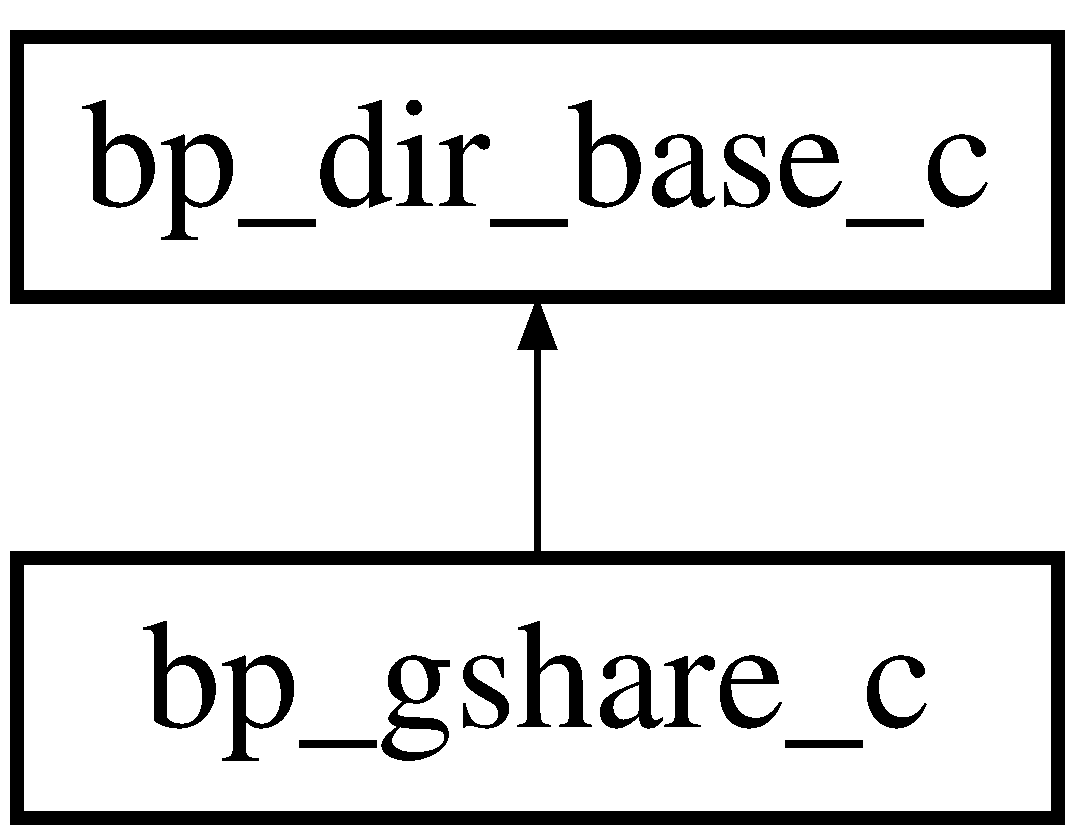
\includegraphics[height=2.000000cm]{classbp__dir__base__c}
\end{center}
\end{figure}
\subsection*{Public Member Functions}
\begin{DoxyCompactItemize}
\item 
\hyperlink{classbp__dir__base__c_ae4cc157dffc44cf03ebf700a0c782a14}{bp\_\-dir\_\-base\_\-c} (\hyperlink{classmacsim__c}{macsim\_\-c} $\ast$simBase)
\item 
\hyperlink{classbp__dir__base__c_a02585e74884b9018ece3dd244b76cc55}{$\sim$bp\_\-dir\_\-base\_\-c} ()
\item 
virtual uns8 \hyperlink{classbp__dir__base__c_a81c9f2b9e8f698581515a764d678bb66}{pred} (\hyperlink{classuop__c}{uop\_\-c} $\ast$uop)=0
\item 
virtual void \hyperlink{classbp__dir__base__c_aef86bf2af2a4ff7b19cbdab57032949f}{update} (\hyperlink{classuop__c}{uop\_\-c} $\ast$uop)=0
\item 
virtual void \hyperlink{classbp__dir__base__c_a9faee1854f637fa57be7094f4b2bc7b9}{recover} (\hyperlink{classrecovery__info__c}{recovery\_\-info\_\-c} $\ast$)=0
\end{DoxyCompactItemize}
\subsection*{Public Attributes}
\begin{DoxyCompactItemize}
\item 
uns8 $\ast$ \hyperlink{classbp__dir__base__c_a8b2a7a886fa7bd761f9ed85dc3d3eb30}{m\_\-pht}
\item 
uns64 \hyperlink{classbp__dir__base__c_a31b1491ed519c0f1b8387b5ac2d29a61}{m\_\-global\_\-hist\_\-64}
\item 
uns32 \hyperlink{classbp__dir__base__c_ac955abfb388ed1d48ebc5eccc916310c}{m\_\-global\_\-hist}
\item 
const char $\ast$ \hyperlink{classbp__dir__base__c_a22d913a24f3144c33794b7440cf8d50c}{m\_\-name}
\end{DoxyCompactItemize}
\subsection*{Protected Attributes}
\begin{DoxyCompactItemize}
\item 
\hyperlink{classmacsim__c}{macsim\_\-c} $\ast$ \hyperlink{classbp__dir__base__c_a8d9e0f72bab48735f49fab60bd2fe0df}{m\_\-simBase}
\end{DoxyCompactItemize}
\subsection*{Private Member Functions}
\begin{DoxyCompactItemize}
\item 
\hyperlink{classbp__dir__base__c_a3d9afa9a22044fc361455c7335dd0979}{bp\_\-dir\_\-base\_\-c} (const \hyperlink{classbp__dir__base__c}{bp\_\-dir\_\-base\_\-c} \&rhs)
\item 
\hyperlink{classbp__dir__base__c}{bp\_\-dir\_\-base\_\-c} \& \hyperlink{classbp__dir__base__c_a9030ec391bf019913c0111651e38591b}{operator=} (const \hyperlink{classbp__dir__base__c}{bp\_\-dir\_\-base\_\-c} \&rhs)
\end{DoxyCompactItemize}


\subsection{Detailed Description}
Branch predictor base class. Branch predictor base Class. Other branch predictors need to inherit this base class. 

\subsection{Constructor \& Destructor Documentation}
\hypertarget{classbp__dir__base__c_ae4cc157dffc44cf03ebf700a0c782a14}{
\index{bp\_\-dir\_\-base\_\-c@{bp\_\-dir\_\-base\_\-c}!bp\_\-dir\_\-base\_\-c@{bp\_\-dir\_\-base\_\-c}}
\index{bp\_\-dir\_\-base\_\-c@{bp\_\-dir\_\-base\_\-c}!bp_dir_base_c@{bp\_\-dir\_\-base\_\-c}}
\subsubsection[{bp\_\-dir\_\-base\_\-c}]{\setlength{\rightskip}{0pt plus 5cm}bp\_\-dir\_\-base\_\-c::bp\_\-dir\_\-base\_\-c (
\begin{DoxyParamCaption}
\item[{{\bf macsim\_\-c} $\ast$}]{ simBase}
\end{DoxyParamCaption}
)}}
\label{classbp__dir__base__c_ae4cc157dffc44cf03ebf700a0c782a14}
Branch predictor class constructor \hypertarget{classbp__dir__base__c_a02585e74884b9018ece3dd244b76cc55}{
\index{bp\_\-dir\_\-base\_\-c@{bp\_\-dir\_\-base\_\-c}!$\sim$bp\_\-dir\_\-base\_\-c@{$\sim$bp\_\-dir\_\-base\_\-c}}
\index{$\sim$bp\_\-dir\_\-base\_\-c@{$\sim$bp\_\-dir\_\-base\_\-c}!bp_dir_base_c@{bp\_\-dir\_\-base\_\-c}}
\subsubsection[{$\sim$bp\_\-dir\_\-base\_\-c}]{\setlength{\rightskip}{0pt plus 5cm}bp\_\-dir\_\-base\_\-c::$\sim$bp\_\-dir\_\-base\_\-c (
\begin{DoxyParamCaption}
{}
\end{DoxyParamCaption}
)}}
\label{classbp__dir__base__c_a02585e74884b9018ece3dd244b76cc55}
Branch predictor class destructor \hypertarget{classbp__dir__base__c_a3d9afa9a22044fc361455c7335dd0979}{
\index{bp\_\-dir\_\-base\_\-c@{bp\_\-dir\_\-base\_\-c}!bp\_\-dir\_\-base\_\-c@{bp\_\-dir\_\-base\_\-c}}
\index{bp\_\-dir\_\-base\_\-c@{bp\_\-dir\_\-base\_\-c}!bp_dir_base_c@{bp\_\-dir\_\-base\_\-c}}
\subsubsection[{bp\_\-dir\_\-base\_\-c}]{\setlength{\rightskip}{0pt plus 5cm}bp\_\-dir\_\-base\_\-c::bp\_\-dir\_\-base\_\-c (
\begin{DoxyParamCaption}
\item[{const {\bf bp\_\-dir\_\-base\_\-c} \&}]{ rhs}
\end{DoxyParamCaption}
)\hspace{0.3cm}{\ttfamily  \mbox{[}private\mbox{]}}}}
\label{classbp__dir__base__c_a3d9afa9a22044fc361455c7335dd0979}
Private constructor Do not implement 

\subsection{Member Function Documentation}
\hypertarget{classbp__dir__base__c_a9030ec391bf019913c0111651e38591b}{
\index{bp\_\-dir\_\-base\_\-c@{bp\_\-dir\_\-base\_\-c}!operator=@{operator=}}
\index{operator=@{operator=}!bp_dir_base_c@{bp\_\-dir\_\-base\_\-c}}
\subsubsection[{operator=}]{\setlength{\rightskip}{0pt plus 5cm}{\bf bp\_\-dir\_\-base\_\-c}\& bp\_\-dir\_\-base\_\-c::operator= (
\begin{DoxyParamCaption}
\item[{const {\bf bp\_\-dir\_\-base\_\-c} \&}]{ rhs}
\end{DoxyParamCaption}
)\hspace{0.3cm}{\ttfamily  \mbox{[}private\mbox{]}}}}
\label{classbp__dir__base__c_a9030ec391bf019913c0111651e38591b}
Overridden operator = \hypertarget{classbp__dir__base__c_a81c9f2b9e8f698581515a764d678bb66}{
\index{bp\_\-dir\_\-base\_\-c@{bp\_\-dir\_\-base\_\-c}!pred@{pred}}
\index{pred@{pred}!bp_dir_base_c@{bp\_\-dir\_\-base\_\-c}}
\subsubsection[{pred}]{\setlength{\rightskip}{0pt plus 5cm}virtual uns8 bp\_\-dir\_\-base\_\-c::pred (
\begin{DoxyParamCaption}
\item[{{\bf uop\_\-c} $\ast$}]{ uop}
\end{DoxyParamCaption}
)\hspace{0.3cm}{\ttfamily  \mbox{[}pure virtual\mbox{]}}}}
\label{classbp__dir__base__c_a81c9f2b9e8f698581515a764d678bb66}
Predict a branch instruction 

Implemented in \hyperlink{classbp__gshare__c_a692880676e5f5a6039832c07a2b5e206}{bp\_\-gshare\_\-c}.

\hypertarget{classbp__dir__base__c_a9faee1854f637fa57be7094f4b2bc7b9}{
\index{bp\_\-dir\_\-base\_\-c@{bp\_\-dir\_\-base\_\-c}!recover@{recover}}
\index{recover@{recover}!bp_dir_base_c@{bp\_\-dir\_\-base\_\-c}}
\subsubsection[{recover}]{\setlength{\rightskip}{0pt plus 5cm}virtual void bp\_\-dir\_\-base\_\-c::recover (
\begin{DoxyParamCaption}
\item[{{\bf recovery\_\-info\_\-c} $\ast$}]{}
\end{DoxyParamCaption}
)\hspace{0.3cm}{\ttfamily  \mbox{[}pure virtual\mbox{]}}}}
\label{classbp__dir__base__c_a9faee1854f637fa57be7094f4b2bc7b9}
Called to recover the bp when a misprediction is realized 

Implemented in \hyperlink{classbp__gshare__c_aa7345e7c9919f2e75bafb7f85e34f6f0}{bp\_\-gshare\_\-c}.

\hypertarget{classbp__dir__base__c_aef86bf2af2a4ff7b19cbdab57032949f}{
\index{bp\_\-dir\_\-base\_\-c@{bp\_\-dir\_\-base\_\-c}!update@{update}}
\index{update@{update}!bp_dir_base_c@{bp\_\-dir\_\-base\_\-c}}
\subsubsection[{update}]{\setlength{\rightskip}{0pt plus 5cm}virtual void bp\_\-dir\_\-base\_\-c::update (
\begin{DoxyParamCaption}
\item[{{\bf uop\_\-c} $\ast$}]{ uop}
\end{DoxyParamCaption}
)\hspace{0.3cm}{\ttfamily  \mbox{[}pure virtual\mbox{]}}}}
\label{classbp__dir__base__c_aef86bf2af2a4ff7b19cbdab57032949f}
Update branch predictor when a branch instruction is resolved. 

Implemented in \hyperlink{classbp__gshare__c_a7f4c0fb922d3640acd10477ff806b91e}{bp\_\-gshare\_\-c}.



\subsection{Member Data Documentation}
\hypertarget{classbp__dir__base__c_ac955abfb388ed1d48ebc5eccc916310c}{
\index{bp\_\-dir\_\-base\_\-c@{bp\_\-dir\_\-base\_\-c}!m\_\-global\_\-hist@{m\_\-global\_\-hist}}
\index{m\_\-global\_\-hist@{m\_\-global\_\-hist}!bp_dir_base_c@{bp\_\-dir\_\-base\_\-c}}
\subsubsection[{m\_\-global\_\-hist}]{\setlength{\rightskip}{0pt plus 5cm}uns32 {\bf bp\_\-dir\_\-base\_\-c::m\_\-global\_\-hist}}}
\label{classbp__dir__base__c_ac955abfb388ed1d48ebc5eccc916310c}
global branch history (32-\/bit) \hypertarget{classbp__dir__base__c_a31b1491ed519c0f1b8387b5ac2d29a61}{
\index{bp\_\-dir\_\-base\_\-c@{bp\_\-dir\_\-base\_\-c}!m\_\-global\_\-hist\_\-64@{m\_\-global\_\-hist\_\-64}}
\index{m\_\-global\_\-hist\_\-64@{m\_\-global\_\-hist\_\-64}!bp_dir_base_c@{bp\_\-dir\_\-base\_\-c}}
\subsubsection[{m\_\-global\_\-hist\_\-64}]{\setlength{\rightskip}{0pt plus 5cm}uns64 {\bf bp\_\-dir\_\-base\_\-c::m\_\-global\_\-hist\_\-64}}}
\label{classbp__dir__base__c_a31b1491ed519c0f1b8387b5ac2d29a61}
global branch history (64-\/bit) \hypertarget{classbp__dir__base__c_a22d913a24f3144c33794b7440cf8d50c}{
\index{bp\_\-dir\_\-base\_\-c@{bp\_\-dir\_\-base\_\-c}!m\_\-name@{m\_\-name}}
\index{m\_\-name@{m\_\-name}!bp_dir_base_c@{bp\_\-dir\_\-base\_\-c}}
\subsubsection[{m\_\-name}]{\setlength{\rightskip}{0pt plus 5cm}const char$\ast$ {\bf bp\_\-dir\_\-base\_\-c::m\_\-name}}}
\label{classbp__dir__base__c_a22d913a24f3144c33794b7440cf8d50c}
branch predictor name \hypertarget{classbp__dir__base__c_a8b2a7a886fa7bd761f9ed85dc3d3eb30}{
\index{bp\_\-dir\_\-base\_\-c@{bp\_\-dir\_\-base\_\-c}!m\_\-pht@{m\_\-pht}}
\index{m\_\-pht@{m\_\-pht}!bp_dir_base_c@{bp\_\-dir\_\-base\_\-c}}
\subsubsection[{m\_\-pht}]{\setlength{\rightskip}{0pt plus 5cm}uns8$\ast$ {\bf bp\_\-dir\_\-base\_\-c::m\_\-pht}}}
\label{classbp__dir__base__c_a8b2a7a886fa7bd761f9ed85dc3d3eb30}
branch history table \hypertarget{classbp__dir__base__c_a8d9e0f72bab48735f49fab60bd2fe0df}{
\index{bp\_\-dir\_\-base\_\-c@{bp\_\-dir\_\-base\_\-c}!m\_\-simBase@{m\_\-simBase}}
\index{m\_\-simBase@{m\_\-simBase}!bp_dir_base_c@{bp\_\-dir\_\-base\_\-c}}
\subsubsection[{m\_\-simBase}]{\setlength{\rightskip}{0pt plus 5cm}{\bf macsim\_\-c}$\ast$ {\bf bp\_\-dir\_\-base\_\-c::m\_\-simBase}\hspace{0.3cm}{\ttfamily  \mbox{[}protected\mbox{]}}}}
\label{classbp__dir__base__c_a8d9e0f72bab48735f49fab60bd2fe0df}
\hyperlink{classmacsim__c}{macsim\_\-c} base class for simulation globals 

The documentation for this class was generated from the following files:\begin{DoxyCompactItemize}
\item 
bp.h\item 
bp.cc\end{DoxyCompactItemize}

\hypertarget{classbp__gshare__c}{
\section{bp\_\-gshare\_\-c Class Reference}
\label{classbp__gshare__c}\index{bp\_\-gshare\_\-c@{bp\_\-gshare\_\-c}}
}


Gshare branch predictor.  




{\ttfamily \#include $<$bp\_\-gshare.h$>$}

Inheritance diagram for bp\_\-gshare\_\-c:\begin{figure}[H]
\begin{center}
\leavevmode
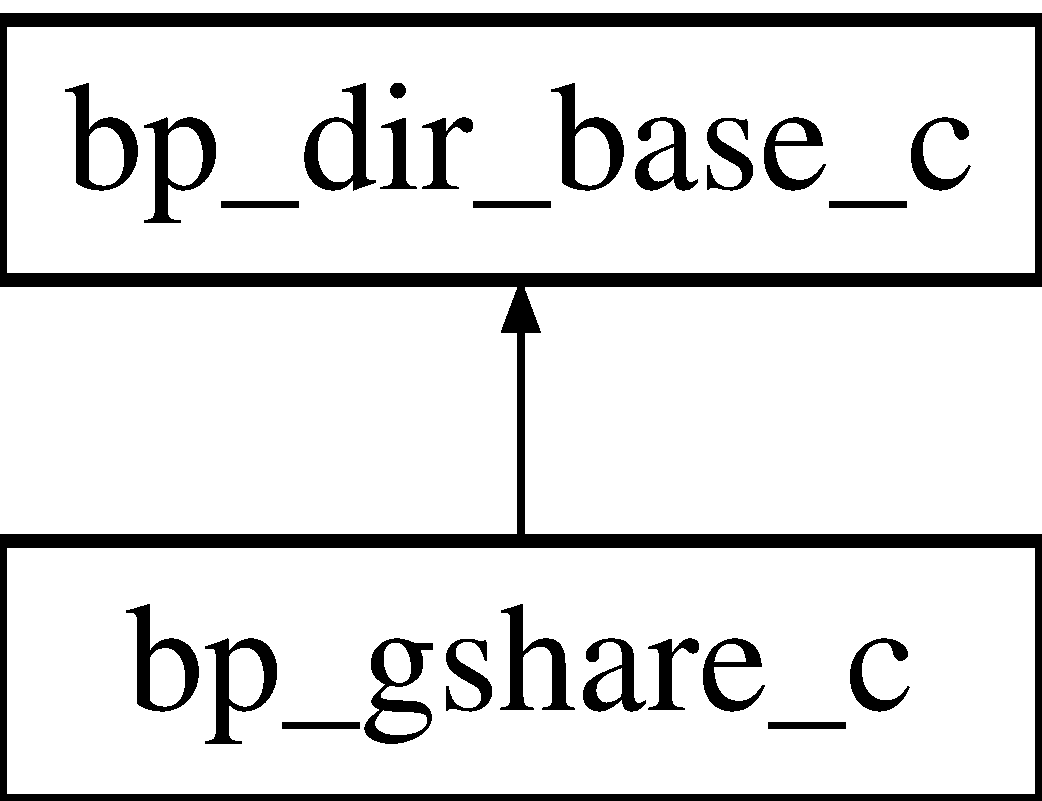
\includegraphics[height=2.000000cm]{classbp__gshare__c}
\end{center}
\end{figure}
\subsection*{Public Member Functions}
\begin{DoxyCompactItemize}
\item 
\hyperlink{classbp__gshare__c_ab4cda4c326dda86ff4724bb77561a4a5}{bp\_\-gshare\_\-c} (\hyperlink{classmacsim__c}{macsim\_\-c} $\ast$simBase)
\item 
\hyperlink{classbp__gshare__c_a75b2b0bc2ca50a7216d8e06884c499ce}{$\sim$bp\_\-gshare\_\-c} (void)
\item 
uns8 \hyperlink{classbp__gshare__c_a692880676e5f5a6039832c07a2b5e206}{pred} (\hyperlink{classuop__c}{uop\_\-c} $\ast$uop)
\item 
void \hyperlink{classbp__gshare__c_a7f4c0fb922d3640acd10477ff806b91e}{update} (\hyperlink{classuop__c}{uop\_\-c} $\ast$uop)
\item 
void \hyperlink{classbp__gshare__c_aa7345e7c9919f2e75bafb7f85e34f6f0}{recover} (\hyperlink{classrecovery__info__c}{recovery\_\-info\_\-c} $\ast$recovery\_\-info)
\end{DoxyCompactItemize}
\subsection*{Private Member Functions}
\begin{DoxyCompactItemize}
\item 
\hyperlink{classbp__gshare__c_a3346112628e7f02012040181964c482d}{bp\_\-gshare\_\-c} (const \hyperlink{classbp__gshare__c}{bp\_\-gshare\_\-c} \&rhs)
\item 
const \hyperlink{classbp__gshare__c}{bp\_\-gshare\_\-c} \& \hyperlink{classbp__gshare__c_aa8a28e878a8f95386cc166bf4e18c980}{operator=} (const \hyperlink{classbp__gshare__c}{bp\_\-gshare\_\-c} \&rhs)
\end{DoxyCompactItemize}


\subsection{Detailed Description}
Gshare branch predictor. Gshare branch predictor class 

\subsection{Constructor \& Destructor Documentation}
\hypertarget{classbp__gshare__c_ab4cda4c326dda86ff4724bb77561a4a5}{
\index{bp\_\-gshare\_\-c@{bp\_\-gshare\_\-c}!bp\_\-gshare\_\-c@{bp\_\-gshare\_\-c}}
\index{bp\_\-gshare\_\-c@{bp\_\-gshare\_\-c}!bp_gshare_c@{bp\_\-gshare\_\-c}}
\subsubsection[{bp\_\-gshare\_\-c}]{\setlength{\rightskip}{0pt plus 5cm}bp\_\-gshare\_\-c::bp\_\-gshare\_\-c (
\begin{DoxyParamCaption}
\item[{{\bf macsim\_\-c} $\ast$}]{ simBase}
\end{DoxyParamCaption}
)}}
\label{classbp__gshare__c_ab4cda4c326dda86ff4724bb77561a4a5}
Gshare BP constructor \hypertarget{classbp__gshare__c_a75b2b0bc2ca50a7216d8e06884c499ce}{
\index{bp\_\-gshare\_\-c@{bp\_\-gshare\_\-c}!$\sim$bp\_\-gshare\_\-c@{$\sim$bp\_\-gshare\_\-c}}
\index{$\sim$bp\_\-gshare\_\-c@{$\sim$bp\_\-gshare\_\-c}!bp_gshare_c@{bp\_\-gshare\_\-c}}
\subsubsection[{$\sim$bp\_\-gshare\_\-c}]{\setlength{\rightskip}{0pt plus 5cm}bp\_\-gshare\_\-c::$\sim$bp\_\-gshare\_\-c (
\begin{DoxyParamCaption}
\item[{void}]{}
\end{DoxyParamCaption}
)\hspace{0.3cm}{\ttfamily  \mbox{[}inline\mbox{]}}}}
\label{classbp__gshare__c_a75b2b0bc2ca50a7216d8e06884c499ce}
Gshare BP destructor \hypertarget{classbp__gshare__c_a3346112628e7f02012040181964c482d}{
\index{bp\_\-gshare\_\-c@{bp\_\-gshare\_\-c}!bp\_\-gshare\_\-c@{bp\_\-gshare\_\-c}}
\index{bp\_\-gshare\_\-c@{bp\_\-gshare\_\-c}!bp_gshare_c@{bp\_\-gshare\_\-c}}
\subsubsection[{bp\_\-gshare\_\-c}]{\setlength{\rightskip}{0pt plus 5cm}bp\_\-gshare\_\-c::bp\_\-gshare\_\-c (
\begin{DoxyParamCaption}
\item[{const {\bf bp\_\-gshare\_\-c} \&}]{ rhs}
\end{DoxyParamCaption}
)\hspace{0.3cm}{\ttfamily  \mbox{[}private\mbox{]}}}}
\label{classbp__gshare__c_a3346112628e7f02012040181964c482d}
Private constructor Do not implement 

\subsection{Member Function Documentation}
\hypertarget{classbp__gshare__c_aa8a28e878a8f95386cc166bf4e18c980}{
\index{bp\_\-gshare\_\-c@{bp\_\-gshare\_\-c}!operator=@{operator=}}
\index{operator=@{operator=}!bp_gshare_c@{bp\_\-gshare\_\-c}}
\subsubsection[{operator=}]{\setlength{\rightskip}{0pt plus 5cm}const {\bf bp\_\-gshare\_\-c}\& bp\_\-gshare\_\-c::operator= (
\begin{DoxyParamCaption}
\item[{const {\bf bp\_\-gshare\_\-c} \&}]{ rhs}
\end{DoxyParamCaption}
)\hspace{0.3cm}{\ttfamily  \mbox{[}private\mbox{]}}}}
\label{classbp__gshare__c_aa8a28e878a8f95386cc166bf4e18c980}
Overridden operator = \hypertarget{classbp__gshare__c_a692880676e5f5a6039832c07a2b5e206}{
\index{bp\_\-gshare\_\-c@{bp\_\-gshare\_\-c}!pred@{pred}}
\index{pred@{pred}!bp_gshare_c@{bp\_\-gshare\_\-c}}
\subsubsection[{pred}]{\setlength{\rightskip}{0pt plus 5cm}uns8 bp\_\-gshare\_\-c::pred (
\begin{DoxyParamCaption}
\item[{{\bf uop\_\-c} $\ast$}]{ uop}
\end{DoxyParamCaption}
)\hspace{0.3cm}{\ttfamily  \mbox{[}virtual\mbox{]}}}}
\label{classbp__gshare__c_a692880676e5f5a6039832c07a2b5e206}
Predict a branch instruction 

Implements \hyperlink{classbp__dir__base__c_a81c9f2b9e8f698581515a764d678bb66}{bp\_\-dir\_\-base\_\-c}.

\hypertarget{classbp__gshare__c_aa7345e7c9919f2e75bafb7f85e34f6f0}{
\index{bp\_\-gshare\_\-c@{bp\_\-gshare\_\-c}!recover@{recover}}
\index{recover@{recover}!bp_gshare_c@{bp\_\-gshare\_\-c}}
\subsubsection[{recover}]{\setlength{\rightskip}{0pt plus 5cm}void bp\_\-gshare\_\-c::recover (
\begin{DoxyParamCaption}
\item[{{\bf recovery\_\-info\_\-c} $\ast$}]{ recovery\_\-info}
\end{DoxyParamCaption}
)\hspace{0.3cm}{\ttfamily  \mbox{[}virtual\mbox{]}}}}
\label{classbp__gshare__c_aa7345e7c9919f2e75bafb7f85e34f6f0}
Called to recover the bp when a misprediction is realized 

Implements \hyperlink{classbp__dir__base__c_a9faee1854f637fa57be7094f4b2bc7b9}{bp\_\-dir\_\-base\_\-c}.

\hypertarget{classbp__gshare__c_a7f4c0fb922d3640acd10477ff806b91e}{
\index{bp\_\-gshare\_\-c@{bp\_\-gshare\_\-c}!update@{update}}
\index{update@{update}!bp_gshare_c@{bp\_\-gshare\_\-c}}
\subsubsection[{update}]{\setlength{\rightskip}{0pt plus 5cm}void bp\_\-gshare\_\-c::update (
\begin{DoxyParamCaption}
\item[{{\bf uop\_\-c} $\ast$}]{ uop}
\end{DoxyParamCaption}
)\hspace{0.3cm}{\ttfamily  \mbox{[}virtual\mbox{]}}}}
\label{classbp__gshare__c_a7f4c0fb922d3640acd10477ff806b91e}
Update branch predictor when a branch instruction is resolved. 

Implements \hyperlink{classbp__dir__base__c_aef86bf2af2a4ff7b19cbdab57032949f}{bp\_\-dir\_\-base\_\-c}.



The documentation for this class was generated from the following files:\begin{DoxyCompactItemize}
\item 
bp\_\-gshare.h\item 
bp\_\-gshare.cc\end{DoxyCompactItemize}

\hypertarget{classbp__recovery__info__c}{
\section{bp\_\-recovery\_\-info\_\-c Class Reference}
\label{classbp__recovery__info__c}\index{bp\_\-recovery\_\-info\_\-c@{bp\_\-recovery\_\-info\_\-c}}
}


Branch recovery information class.  




{\ttfamily \#include $<$bp.h$>$}

\subsection*{Public Member Functions}
\begin{DoxyCompactItemize}
\item 
\hyperlink{classbp__recovery__info__c_a04e835b432804f946b1a846240e176ba}{bp\_\-recovery\_\-info\_\-c} ()
\item 
\hyperlink{classbp__recovery__info__c_a23043b47ebad45830826a086b9ff839a}{$\sim$bp\_\-recovery\_\-info\_\-c} ()
\end{DoxyCompactItemize}
\subsection*{Public Attributes}
\begin{DoxyCompactItemize}
\item 
Counter \hyperlink{classbp__recovery__info__c_a00230943e8204144e777bd49d036f9df}{m\_\-recovery\_\-cycle}
\item 
Addr \hyperlink{classbp__recovery__info__c_a6dfab69054850067ef95b38faf85cec1}{m\_\-recovery\_\-fetch\_\-addr}
\item 
Counter \hyperlink{classbp__recovery__info__c_a4d165d8ea37c2a80f93385010f780b93}{m\_\-recovery\_\-op\_\-num}
\item 
Counter \hyperlink{classbp__recovery__info__c_afdb299ba15294f1f1681f8e363ffcdbd}{m\_\-recovery\_\-cf\_\-type}
\item 
\hyperlink{classrecovery__info__c}{recovery\_\-info\_\-c} $\ast$ \hyperlink{classbp__recovery__info__c_a8addc9c062b96ddfdec35d817d215117}{m\_\-recovery\_\-info}
\item 
Counter \hyperlink{classbp__recovery__info__c_ae42bca851549fbe1dfbb3b3bb02854af}{m\_\-redirect\_\-cycle}
\item 
Addr \hyperlink{classbp__recovery__info__c_aa037c488f3aec47db7b5b19eed5ee682}{m\_\-redirect\_\-fetch\_\-addr}
\item 
Counter \hyperlink{classbp__recovery__info__c_ad7f574a8e5006bc0f34757bfcd0642b7}{m\_\-redirect\_\-op\_\-num}
\end{DoxyCompactItemize}


\subsection{Detailed Description}
Branch recovery information class. recover: when a branch is mispredicted redirect: when a front-\/end is not fetching correct instructions such as btb miss 

\subsection{Constructor \& Destructor Documentation}
\hypertarget{classbp__recovery__info__c_a04e835b432804f946b1a846240e176ba}{
\index{bp\_\-recovery\_\-info\_\-c@{bp\_\-recovery\_\-info\_\-c}!bp\_\-recovery\_\-info\_\-c@{bp\_\-recovery\_\-info\_\-c}}
\index{bp\_\-recovery\_\-info\_\-c@{bp\_\-recovery\_\-info\_\-c}!bp_recovery_info_c@{bp\_\-recovery\_\-info\_\-c}}
\subsubsection[{bp\_\-recovery\_\-info\_\-c}]{\setlength{\rightskip}{0pt plus 5cm}bp\_\-recovery\_\-info\_\-c::bp\_\-recovery\_\-info\_\-c (
\begin{DoxyParamCaption}
{}
\end{DoxyParamCaption}
)}}
\label{classbp__recovery__info__c_a04e835b432804f946b1a846240e176ba}
Mispredicted branch recovery information Class constructor \hypertarget{classbp__recovery__info__c_a23043b47ebad45830826a086b9ff839a}{
\index{bp\_\-recovery\_\-info\_\-c@{bp\_\-recovery\_\-info\_\-c}!$\sim$bp\_\-recovery\_\-info\_\-c@{$\sim$bp\_\-recovery\_\-info\_\-c}}
\index{$\sim$bp\_\-recovery\_\-info\_\-c@{$\sim$bp\_\-recovery\_\-info\_\-c}!bp_recovery_info_c@{bp\_\-recovery\_\-info\_\-c}}
\subsubsection[{$\sim$bp\_\-recovery\_\-info\_\-c}]{\setlength{\rightskip}{0pt plus 5cm}bp\_\-recovery\_\-info\_\-c::$\sim$bp\_\-recovery\_\-info\_\-c (
\begin{DoxyParamCaption}
{}
\end{DoxyParamCaption}
)}}
\label{classbp__recovery__info__c_a23043b47ebad45830826a086b9ff839a}
Mispredicted branch recovery information Class destructor 

\subsection{Member Data Documentation}
\hypertarget{classbp__recovery__info__c_afdb299ba15294f1f1681f8e363ffcdbd}{
\index{bp\_\-recovery\_\-info\_\-c@{bp\_\-recovery\_\-info\_\-c}!m\_\-recovery\_\-cf\_\-type@{m\_\-recovery\_\-cf\_\-type}}
\index{m\_\-recovery\_\-cf\_\-type@{m\_\-recovery\_\-cf\_\-type}!bp_recovery_info_c@{bp\_\-recovery\_\-info\_\-c}}
\subsubsection[{m\_\-recovery\_\-cf\_\-type}]{\setlength{\rightskip}{0pt plus 5cm}Counter {\bf bp\_\-recovery\_\-info\_\-c::m\_\-recovery\_\-cf\_\-type}}}
\label{classbp__recovery__info__c_afdb299ba15294f1f1681f8e363ffcdbd}
cf\_\-type of op that caused recovery \hypertarget{classbp__recovery__info__c_a00230943e8204144e777bd49d036f9df}{
\index{bp\_\-recovery\_\-info\_\-c@{bp\_\-recovery\_\-info\_\-c}!m\_\-recovery\_\-cycle@{m\_\-recovery\_\-cycle}}
\index{m\_\-recovery\_\-cycle@{m\_\-recovery\_\-cycle}!bp_recovery_info_c@{bp\_\-recovery\_\-info\_\-c}}
\subsubsection[{m\_\-recovery\_\-cycle}]{\setlength{\rightskip}{0pt plus 5cm}Counter {\bf bp\_\-recovery\_\-info\_\-c::m\_\-recovery\_\-cycle}}}
\label{classbp__recovery__info__c_a00230943e8204144e777bd49d036f9df}
cycle that begins misprediction recovery \hypertarget{classbp__recovery__info__c_a6dfab69054850067ef95b38faf85cec1}{
\index{bp\_\-recovery\_\-info\_\-c@{bp\_\-recovery\_\-info\_\-c}!m\_\-recovery\_\-fetch\_\-addr@{m\_\-recovery\_\-fetch\_\-addr}}
\index{m\_\-recovery\_\-fetch\_\-addr@{m\_\-recovery\_\-fetch\_\-addr}!bp_recovery_info_c@{bp\_\-recovery\_\-info\_\-c}}
\subsubsection[{m\_\-recovery\_\-fetch\_\-addr}]{\setlength{\rightskip}{0pt plus 5cm}Addr {\bf bp\_\-recovery\_\-info\_\-c::m\_\-recovery\_\-fetch\_\-addr}}}
\label{classbp__recovery__info__c_a6dfab69054850067ef95b38faf85cec1}
address to redirect the istream \hypertarget{classbp__recovery__info__c_a8addc9c062b96ddfdec35d817d215117}{
\index{bp\_\-recovery\_\-info\_\-c@{bp\_\-recovery\_\-info\_\-c}!m\_\-recovery\_\-info@{m\_\-recovery\_\-info}}
\index{m\_\-recovery\_\-info@{m\_\-recovery\_\-info}!bp_recovery_info_c@{bp\_\-recovery\_\-info\_\-c}}
\subsubsection[{m\_\-recovery\_\-info}]{\setlength{\rightskip}{0pt plus 5cm}{\bf recovery\_\-info\_\-c}$\ast$ {\bf bp\_\-recovery\_\-info\_\-c::m\_\-recovery\_\-info}}}
\label{classbp__recovery__info__c_a8addc9c062b96ddfdec35d817d215117}
information about the op causing the recovery \hypertarget{classbp__recovery__info__c_a4d165d8ea37c2a80f93385010f780b93}{
\index{bp\_\-recovery\_\-info\_\-c@{bp\_\-recovery\_\-info\_\-c}!m\_\-recovery\_\-op\_\-num@{m\_\-recovery\_\-op\_\-num}}
\index{m\_\-recovery\_\-op\_\-num@{m\_\-recovery\_\-op\_\-num}!bp_recovery_info_c@{bp\_\-recovery\_\-info\_\-c}}
\subsubsection[{m\_\-recovery\_\-op\_\-num}]{\setlength{\rightskip}{0pt plus 5cm}Counter {\bf bp\_\-recovery\_\-info\_\-c::m\_\-recovery\_\-op\_\-num}}}
\label{classbp__recovery__info__c_a4d165d8ea37c2a80f93385010f780b93}
op\_\-num of op that caused recovery \hypertarget{classbp__recovery__info__c_ae42bca851549fbe1dfbb3b3bb02854af}{
\index{bp\_\-recovery\_\-info\_\-c@{bp\_\-recovery\_\-info\_\-c}!m\_\-redirect\_\-cycle@{m\_\-redirect\_\-cycle}}
\index{m\_\-redirect\_\-cycle@{m\_\-redirect\_\-cycle}!bp_recovery_info_c@{bp\_\-recovery\_\-info\_\-c}}
\subsubsection[{m\_\-redirect\_\-cycle}]{\setlength{\rightskip}{0pt plus 5cm}Counter {\bf bp\_\-recovery\_\-info\_\-c::m\_\-redirect\_\-cycle}}}
\label{classbp__recovery__info__c_ae42bca851549fbe1dfbb3b3bb02854af}
cycle that begins a redirection (eg. btb miss) \hypertarget{classbp__recovery__info__c_aa037c488f3aec47db7b5b19eed5ee682}{
\index{bp\_\-recovery\_\-info\_\-c@{bp\_\-recovery\_\-info\_\-c}!m\_\-redirect\_\-fetch\_\-addr@{m\_\-redirect\_\-fetch\_\-addr}}
\index{m\_\-redirect\_\-fetch\_\-addr@{m\_\-redirect\_\-fetch\_\-addr}!bp_recovery_info_c@{bp\_\-recovery\_\-info\_\-c}}
\subsubsection[{m\_\-redirect\_\-fetch\_\-addr}]{\setlength{\rightskip}{0pt plus 5cm}Addr {\bf bp\_\-recovery\_\-info\_\-c::m\_\-redirect\_\-fetch\_\-addr}}}
\label{classbp__recovery__info__c_aa037c488f3aec47db7b5b19eed5ee682}
address to redirect to \hypertarget{classbp__recovery__info__c_ad7f574a8e5006bc0f34757bfcd0642b7}{
\index{bp\_\-recovery\_\-info\_\-c@{bp\_\-recovery\_\-info\_\-c}!m\_\-redirect\_\-op\_\-num@{m\_\-redirect\_\-op\_\-num}}
\index{m\_\-redirect\_\-op\_\-num@{m\_\-redirect\_\-op\_\-num}!bp_recovery_info_c@{bp\_\-recovery\_\-info\_\-c}}
\subsubsection[{m\_\-redirect\_\-op\_\-num}]{\setlength{\rightskip}{0pt plus 5cm}Counter {\bf bp\_\-recovery\_\-info\_\-c::m\_\-redirect\_\-op\_\-num}}}
\label{classbp__recovery__info__c_ad7f574a8e5006bc0f34757bfcd0642b7}
op\_\-num of op that caused redirect 

The documentation for this class was generated from the following files:\begin{DoxyCompactItemize}
\item 
bp.h\item 
bp.cc\end{DoxyCompactItemize}

\hypertarget{classbp__targ__c}{
\section{bp\_\-targ\_\-c Class Reference}
\label{classbp__targ__c}\index{bp\_\-targ\_\-c@{bp\_\-targ\_\-c}}
}


{\ttfamily \#include $<$bp\_\-targ.h$>$}

\subsection*{Public Member Functions}
\begin{DoxyCompactItemize}
\item 
\hypertarget{classbp__targ__c_a84d6b601bdabdd5ea804e83cf8a782a4}{
{\bfseries bp\_\-targ\_\-c} (uns core\_\-id, \hyperlink{classmacsim__c}{macsim\_\-c} $\ast$simBase)}
\label{classbp__targ__c_a84d6b601bdabdd5ea804e83cf8a782a4}

\item 
\hypertarget{classbp__targ__c_a50e579ddc1d8b2014955649535a4ab8c}{
Addr {\bfseries pred} (\hyperlink{classuop__c}{uop\_\-c} $\ast$uop)}
\label{classbp__targ__c_a50e579ddc1d8b2014955649535a4ab8c}

\item 
\hypertarget{classbp__targ__c_a855b2b9a8d851976301c29df9de040fc}{
void {\bfseries update} (\hyperlink{classuop__c}{uop\_\-c} $\ast$uop)}
\label{classbp__targ__c_a855b2b9a8d851976301c29df9de040fc}

\end{DoxyCompactItemize}
\subsection*{Protected Attributes}
\begin{DoxyCompactItemize}
\item 
\hypertarget{classbp__targ__c_a8b2a93e731b675e971842e66953e3e6b}{
\hyperlink{classmacsim__c}{macsim\_\-c} $\ast$ {\bfseries m\_\-simBase}}
\label{classbp__targ__c_a8b2a93e731b675e971842e66953e3e6b}

\end{DoxyCompactItemize}
\subsection*{Private Attributes}
\begin{DoxyCompactItemize}
\item 
\hypertarget{classbp__targ__c_a01a71175e81ce237a8db74ea50ee39e7}{
\hyperlink{classcache__c}{cache\_\-c} $\ast$ {\bfseries btb}}
\label{classbp__targ__c_a01a71175e81ce237a8db74ea50ee39e7}

\item 
\hypertarget{classbp__targ__c_ab59c9682db97bf0a992321c89b521993}{
uns {\bfseries m\_\-core\_\-id}}
\label{classbp__targ__c_ab59c9682db97bf0a992321c89b521993}

\end{DoxyCompactItemize}


\subsection{Detailed Description}
Target Buffer BTB modeling 

The documentation for this class was generated from the following files:\begin{DoxyCompactItemize}
\item 
bp\_\-targ.h\item 
bp\_\-targ.cc\end{DoxyCompactItemize}

\hypertarget{classbug__detector__c}{
\section{bug\_\-detector\_\-c Class Reference}
\label{classbug__detector__c}\index{bug\_\-detector\_\-c@{bug\_\-detector\_\-c}}
}


bug detection mechanism  




{\ttfamily \#include $<$bug\_\-detector.h$>$}

\subsection*{Public Member Functions}
\begin{DoxyCompactItemize}
\item 
\hyperlink{classbug__detector__c_a3df8691c8540d84e124b21f963b63b85}{bug\_\-detector\_\-c} (\hyperlink{classmacsim__c}{macsim\_\-c} $\ast$simBase)
\item 
\hyperlink{classbug__detector__c_a099634a48c3bb831ba71e324c715ee07}{$\sim$bug\_\-detector\_\-c} ()
\item 
void \hyperlink{classbug__detector__c_a3437b86d0318c26d6400b6f4720a07a8}{allocate} (\hyperlink{classuop__c}{uop\_\-c} $\ast$uop)
\item 
void \hyperlink{classbug__detector__c_a85401b346bcc130a82efe527c86c93e0}{deallocate} (\hyperlink{classuop__c}{uop\_\-c} $\ast$uop)
\item 
void \hyperlink{classbug__detector__c_adb23aaa4e33a08f4dd92f0767cb17d39}{print} (int core\_\-id, int thread\_\-id)
\item 
\hypertarget{classbug__detector__c_aa51660c5a7b6deb7391480fbe74bbb3a}{
void {\bfseries allocate\_\-noc} (\hyperlink{structmem__req__s}{mem\_\-req\_\-s} $\ast$req)}
\label{classbug__detector__c_aa51660c5a7b6deb7391480fbe74bbb3a}

\item 
\hypertarget{classbug__detector__c_a6a65357fe5803b0a1a3bfb22ffbe1015}{
void {\bfseries deallocate\_\-noc} (\hyperlink{structmem__req__s}{mem\_\-req\_\-s} $\ast$req)}
\label{classbug__detector__c_a6a65357fe5803b0a1a3bfb22ffbe1015}

\item 
\hypertarget{classbug__detector__c_a556e83704342d2a8fc5fd600e0dd8df9}{
void {\bfseries print\_\-noc} ()}
\label{classbug__detector__c_a556e83704342d2a8fc5fd600e0dd8df9}

\end{DoxyCompactItemize}
\subsection*{Private Attributes}
\begin{DoxyCompactItemize}
\item 
int \hyperlink{classbug__detector__c_a3d90d9bf03b550875f24acc533352640}{m\_\-num\_\-core}
\item 
vector$<$ map$<$ \hyperlink{classuop__c}{uop\_\-c} $\ast$, uint64\_\-t $>$ $\ast$ $>$ \hyperlink{classbug__detector__c_a0b23d445e54499579a1126223c119948}{m\_\-uop\_\-table}
\item 
uint64\_\-t $\ast$ \hyperlink{classbug__detector__c_ae1a942538a13d23d8bee7355c7e22e0c}{m\_\-latency\_\-sum}
\item 
uint64\_\-t $\ast$ \hyperlink{classbug__detector__c_a40b39407ec6f0e2e0888cac9a7486453}{m\_\-latency\_\-count}
\item 
unordered\_\-map$<$ \hyperlink{structmem__req__s}{mem\_\-req\_\-s} $\ast$, uint64\_\-t $>$ $\ast$ \hyperlink{classbug__detector__c_a650c89720f96ea9c79230e7341b88885}{m\_\-packet\_\-table}
\item 
\hypertarget{classbug__detector__c_a305a1bee1bec006e7dcbc7fb0645f693}{
\hyperlink{classmacsim__c}{macsim\_\-c} $\ast$ {\bfseries m\_\-simBase}}
\label{classbug__detector__c_a305a1bee1bec006e7dcbc7fb0645f693}

\end{DoxyCompactItemize}


\subsection{Detailed Description}
bug detection mechanism Track each uop and memory reqeust to check where it is stuck 

\subsection{Constructor \& Destructor Documentation}
\hypertarget{classbug__detector__c_a3df8691c8540d84e124b21f963b63b85}{
\index{bug\_\-detector\_\-c@{bug\_\-detector\_\-c}!bug\_\-detector\_\-c@{bug\_\-detector\_\-c}}
\index{bug\_\-detector\_\-c@{bug\_\-detector\_\-c}!bug_detector_c@{bug\_\-detector\_\-c}}
\subsubsection[{bug\_\-detector\_\-c}]{\setlength{\rightskip}{0pt plus 5cm}bug\_\-detector\_\-c::bug\_\-detector\_\-c (
\begin{DoxyParamCaption}
\item[{{\bf macsim\_\-c} $\ast$}]{ simBase}
\end{DoxyParamCaption}
)}}
\label{classbug__detector__c_a3df8691c8540d84e124b21f963b63b85}
Bug detector class constructor \hypertarget{classbug__detector__c_a099634a48c3bb831ba71e324c715ee07}{
\index{bug\_\-detector\_\-c@{bug\_\-detector\_\-c}!$\sim$bug\_\-detector\_\-c@{$\sim$bug\_\-detector\_\-c}}
\index{$\sim$bug\_\-detector\_\-c@{$\sim$bug\_\-detector\_\-c}!bug_detector_c@{bug\_\-detector\_\-c}}
\subsubsection[{$\sim$bug\_\-detector\_\-c}]{\setlength{\rightskip}{0pt plus 5cm}bug\_\-detector\_\-c::$\sim$bug\_\-detector\_\-c (
\begin{DoxyParamCaption}
{}
\end{DoxyParamCaption}
)}}
\label{classbug__detector__c_a099634a48c3bb831ba71e324c715ee07}
Bug detector class destructor 

\subsection{Member Function Documentation}
\hypertarget{classbug__detector__c_a3437b86d0318c26d6400b6f4720a07a8}{
\index{bug\_\-detector\_\-c@{bug\_\-detector\_\-c}!allocate@{allocate}}
\index{allocate@{allocate}!bug_detector_c@{bug\_\-detector\_\-c}}
\subsubsection[{allocate}]{\setlength{\rightskip}{0pt plus 5cm}void bug\_\-detector\_\-c::allocate (
\begin{DoxyParamCaption}
\item[{{\bf uop\_\-c} $\ast$}]{ uop}
\end{DoxyParamCaption}
)}}
\label{classbug__detector__c_a3437b86d0318c26d6400b6f4720a07a8}
When a new uop starts exectuion, record it to the table. \hypertarget{classbug__detector__c_a85401b346bcc130a82efe527c86c93e0}{
\index{bug\_\-detector\_\-c@{bug\_\-detector\_\-c}!deallocate@{deallocate}}
\index{deallocate@{deallocate}!bug_detector_c@{bug\_\-detector\_\-c}}
\subsubsection[{deallocate}]{\setlength{\rightskip}{0pt plus 5cm}void bug\_\-detector\_\-c::deallocate (
\begin{DoxyParamCaption}
\item[{{\bf uop\_\-c} $\ast$}]{ uop}
\end{DoxyParamCaption}
)}}
\label{classbug__detector__c_a85401b346bcc130a82efe527c86c93e0}
When a new uop retires, take this uop out from the table. \hypertarget{classbug__detector__c_adb23aaa4e33a08f4dd92f0767cb17d39}{
\index{bug\_\-detector\_\-c@{bug\_\-detector\_\-c}!print@{print}}
\index{print@{print}!bug_detector_c@{bug\_\-detector\_\-c}}
\subsubsection[{print}]{\setlength{\rightskip}{0pt plus 5cm}void bug\_\-detector\_\-c::print (
\begin{DoxyParamCaption}
\item[{int}]{ core\_\-id, }
\item[{int}]{ thread\_\-id}
\end{DoxyParamCaption}
)}}
\label{classbug__detector__c_adb23aaa4e33a08f4dd92f0767cb17d39}
Print all un-\/retired (might be bug) uops 

\subsection{Member Data Documentation}
\hypertarget{classbug__detector__c_a40b39407ec6f0e2e0888cac9a7486453}{
\index{bug\_\-detector\_\-c@{bug\_\-detector\_\-c}!m\_\-latency\_\-count@{m\_\-latency\_\-count}}
\index{m\_\-latency\_\-count@{m\_\-latency\_\-count}!bug_detector_c@{bug\_\-detector\_\-c}}
\subsubsection[{m\_\-latency\_\-count}]{\setlength{\rightskip}{0pt plus 5cm}uint64\_\-t$\ast$ {\bf bug\_\-detector\_\-c::m\_\-latency\_\-count}\hspace{0.3cm}{\ttfamily  \mbox{[}private\mbox{]}}}}
\label{classbug__detector__c_a40b39407ec6f0e2e0888cac9a7486453}
total uop count \hypertarget{classbug__detector__c_ae1a942538a13d23d8bee7355c7e22e0c}{
\index{bug\_\-detector\_\-c@{bug\_\-detector\_\-c}!m\_\-latency\_\-sum@{m\_\-latency\_\-sum}}
\index{m\_\-latency\_\-sum@{m\_\-latency\_\-sum}!bug_detector_c@{bug\_\-detector\_\-c}}
\subsubsection[{m\_\-latency\_\-sum}]{\setlength{\rightskip}{0pt plus 5cm}uint64\_\-t$\ast$ {\bf bug\_\-detector\_\-c::m\_\-latency\_\-sum}\hspace{0.3cm}{\ttfamily  \mbox{[}private\mbox{]}}}}
\label{classbug__detector__c_ae1a942538a13d23d8bee7355c7e22e0c}
sum of each uop's execution latency \hypertarget{classbug__detector__c_a3d90d9bf03b550875f24acc533352640}{
\index{bug\_\-detector\_\-c@{bug\_\-detector\_\-c}!m\_\-num\_\-core@{m\_\-num\_\-core}}
\index{m\_\-num\_\-core@{m\_\-num\_\-core}!bug_detector_c@{bug\_\-detector\_\-c}}
\subsubsection[{m\_\-num\_\-core}]{\setlength{\rightskip}{0pt plus 5cm}int {\bf bug\_\-detector\_\-c::m\_\-num\_\-core}\hspace{0.3cm}{\ttfamily  \mbox{[}private\mbox{]}}}}
\label{classbug__detector__c_a3d90d9bf03b550875f24acc533352640}
number of simulating cores \hypertarget{classbug__detector__c_a650c89720f96ea9c79230e7341b88885}{
\index{bug\_\-detector\_\-c@{bug\_\-detector\_\-c}!m\_\-packet\_\-table@{m\_\-packet\_\-table}}
\index{m\_\-packet\_\-table@{m\_\-packet\_\-table}!bug_detector_c@{bug\_\-detector\_\-c}}
\subsubsection[{m\_\-packet\_\-table}]{\setlength{\rightskip}{0pt plus 5cm}unordered\_\-map$<${\bf mem\_\-req\_\-s}$\ast$, uint64\_\-t$>$$\ast$ {\bf bug\_\-detector\_\-c::m\_\-packet\_\-table}\hspace{0.3cm}{\ttfamily  \mbox{[}private\mbox{]}}}}
\label{classbug__detector__c_a650c89720f96ea9c79230e7341b88885}
memeory requests in noc \hypertarget{classbug__detector__c_a0b23d445e54499579a1126223c119948}{
\index{bug\_\-detector\_\-c@{bug\_\-detector\_\-c}!m\_\-uop\_\-table@{m\_\-uop\_\-table}}
\index{m\_\-uop\_\-table@{m\_\-uop\_\-table}!bug_detector_c@{bug\_\-detector\_\-c}}
\subsubsection[{m\_\-uop\_\-table}]{\setlength{\rightskip}{0pt plus 5cm}vector$<$map$<${\bf uop\_\-c}$\ast$, uint64\_\-t$>$ $\ast$$>$ {\bf bug\_\-detector\_\-c::m\_\-uop\_\-table}\hspace{0.3cm}{\ttfamily  \mbox{[}private\mbox{]}}}}
\label{classbug__detector__c_a0b23d445e54499579a1126223c119948}
uop table 

The documentation for this class was generated from the following files:\begin{DoxyCompactItemize}
\item 
bug\_\-detector.h\item 
bug\_\-detector.cc\end{DoxyCompactItemize}

\hypertarget{classcache__c}{
\section{cache\_\-c Class Reference}
\label{classcache__c}\index{cache\_\-c@{cache\_\-c}}
}


Cache library class.  




{\ttfamily \#include $<$cache.h$>$}

\subsection*{Public Member Functions}
\begin{DoxyCompactItemize}
\item 
\hyperlink{classcache__c_a06c86665989bfa0caa98f72a3a3c950d}{cache\_\-c} (string name, int num\_\-set, int assoc, int line\_\-size, int data\_\-size, int bank\_\-num, bool cache\_\-by\_\-pass, int core\_\-id, Cache\_\-Type cache\_\-type\_\-info, bool enable\_\-partition, \hyperlink{classmacsim__c}{macsim\_\-c} $\ast$simBase)
\begin{DoxyCompactList}\small\item\em Create a new cache using the configuration sent by the caller. \item\end{DoxyCompactList}\item 
void \hyperlink{classcache__c_a8b93e3ac932635054aa96c3d7a5160fe}{set\_\-core\_\-id} (int c\_\-id)
\begin{DoxyCompactList}\small\item\em Function to assign a core id. \item\end{DoxyCompactList}\item 
void \hyperlink{classcache__c_aee40ee4fac5a59a7ce50f4f12d618b55}{find\_\-tag\_\-and\_\-set} (Addr addr, Addr $\ast$tag, int $\ast$set)
\begin{DoxyCompactList}\small\item\em Function to find tag and set from a given address. \item\end{DoxyCompactList}\item 
void $\ast$ \hyperlink{classcache__c_a09960f86c2e0907c90909562c17c46ef}{access\_\-cache} (Addr addr, Addr $\ast$line\_\-addr, bool update\_\-repl, int appl\_\-id)
\begin{DoxyCompactList}\small\item\em Cache look-\/up based on address. \item\end{DoxyCompactList}\item 
\hypertarget{classcache__c_a0190992dae971c5bd97684dec684e367}{
virtual void {\bfseries update\_\-cache\_\-on\_\-access} (Addr tag, int set, int appl\_\-id)}
\label{classcache__c_a0190992dae971c5bd97684dec684e367}

\item 
virtual void \hyperlink{classcache__c_a906f30d49e5bfe3c1c552c68c88203ad}{update\_\-line\_\-on\_\-hit} (\hyperlink{classcache__entry__c}{cache\_\-entry\_\-c} $\ast$line, int set, int appl\_\-id)
\item 
virtual void \hyperlink{classcache__c_a5cfe0d49b4a6ae4ca824006a002023e2}{update\_\-cache\_\-on\_\-miss} (int set\_\-id, int appl\_\-id)
\item 
virtual void \hyperlink{classcache__c_a8283f21120a7153276b5be44b6b7034d}{update\_\-set\_\-on\_\-replacement} (Addr tag, int appl\_\-id, int set\_\-id, bool gpuline)
\item 
\hypertarget{classcache__c_ac392037a6161e55dc67ddb7485be4d2a}{
virtual \hyperlink{classcache__entry__c}{cache\_\-entry\_\-c} $\ast$ {\bfseries find\_\-replacement\_\-line} (int set, int appl\_\-id)}
\label{classcache__c_ac392037a6161e55dc67ddb7485be4d2a}

\item 
\hyperlink{classcache__entry__c}{cache\_\-entry\_\-c} $\ast$ \hyperlink{classcache__c_a3e2d380dc2c5f843ad62828d8f31459d}{find\_\-replacement\_\-line\_\-from\_\-same\_\-type} (int set, int appl\_\-id, bool gpuline)
\item 
\hypertarget{classcache__c_afeb14b30179d559c79d6c7ec3e95b10d}{
virtual void {\bfseries initialize\_\-cache\_\-line} (\hyperlink{classcache__entry__c}{cache\_\-entry\_\-c} $\ast$ins\_\-line, Addr tag, Addr addr, int appl\_\-id, bool gpuline, int set\_\-id, bool skip)}
\label{classcache__c_afeb14b30179d559c79d6c7ec3e95b10d}

\item 
\hypertarget{classcache__c_ae98115af7993894f39eae1659cd79395}{
void $\ast$ {\bfseries insert\_\-cache} (Addr addr, Addr $\ast$line\_\-addr, Addr $\ast$repl\_\-line, int appl\_\-id, bool gpuline)}
\label{classcache__c_ae98115af7993894f39eae1659cd79395}

\item 
\hypertarget{classcache__c_a3c29085ff7b74414442d41c11b7aaa0f}{
void $\ast$ {\bfseries insert\_\-cache} (Addr addr, Addr $\ast$line\_\-addr, Addr $\ast$repl\_\-line, int appl\_\-id, bool gpuline, bool skip)}
\label{classcache__c_a3c29085ff7b74414442d41c11b7aaa0f}

\item 
bool \hyperlink{classcache__c_aae28d6130baf524f85a58a8e1f26bf95}{null\_\-cache\_\-line\_\-fields} (\hyperlink{classcache__entry__c}{cache\_\-entry\_\-c} $\ast$line)
\begin{DoxyCompactList}\small\item\em Function to null out all fields in the caache line being invalidated. \item\end{DoxyCompactList}\item 
bool \hyperlink{classcache__c_ac3c3a33a6f436e39352ae35d94fd72ec}{invalidate\_\-cache\_\-line} (Addr addr)
\begin{DoxyCompactList}\small\item\em Function to invalidate cache line. \item\end{DoxyCompactList}\item 
Addr \hyperlink{classcache__c_a05aa7422c71bd2538886dc0d8d1718a4}{base\_\-cache\_\-line} (Addr addr)
\begin{DoxyCompactList}\small\item\em Function to return base cache line. \item\end{DoxyCompactList}\item 
void \hyperlink{classcache__c_a73bda6639c0868419508f20a1956ae81}{invalidate\_\-cache} (void)
\begin{DoxyCompactList}\small\item\em Function to null out cache fields. \item\end{DoxyCompactList}\item 
int \hyperlink{classcache__c_aa104a52d1962e786f7e36fe06e08c7d4}{get\_\-bank\_\-num} (Addr addr)
\begin{DoxyCompactList}\small\item\em Function to get bank number for the addr. \item\end{DoxyCompactList}\item 
Counter \hyperlink{classcache__c_af7987c188d853dbe7ca27edbd26e5819}{find\_\-min\_\-lru} (int set)
\begin{DoxyCompactList}\small\item\em Function to find the line with least access time in the set. \item\end{DoxyCompactList}\item 
void \hyperlink{classcache__c_ad7e41459c6f50c4cd1f3b41cf7b3811e}{print\_\-info} (int id)
\end{DoxyCompactItemize}
\subsection*{Public Attributes}
\begin{DoxyCompactItemize}
\item 
Cache\_\-Type \hyperlink{classcache__c_a5d3a5366674d862f4818e2980af21b50}{m\_\-cache\_\-type}
\end{DoxyCompactItemize}
\subsection*{Protected Attributes}
\begin{DoxyCompactItemize}
\item 
string \hyperlink{classcache__c_a6feda51818d2216832b855cd4a36d400}{m\_\-name}
\item 
int \hyperlink{classcache__c_a30907cdb4c4078c28d1210e535d1acdb}{m\_\-data\_\-size}
\item 
int \hyperlink{classcache__c_a1baa2f851f435fb5ecd11ead4f3dcc66}{m\_\-assoc}
\item 
int \hyperlink{classcache__c_a1e7c693df55654e3c37aa5e8fcf80272}{m\_\-num\_\-sets}
\item 
int \hyperlink{classcache__c_ae4a82fe5d53c5b2b6382295628852888}{m\_\-line\_\-size}
\item 
int \hyperlink{classcache__c_a9ad9a67a9325d355365b35aed1c4a77c}{m\_\-set\_\-bits}
\item 
int \hyperlink{classcache__c_a6e91a255d6cc037331a5f2c7e542ea46}{m\_\-shift\_\-bits}
\item 
Addr \hyperlink{classcache__c_a4d0db9dfcbb07b40e41881ca8579f7b0}{m\_\-set\_\-mask}
\item 
Addr \hyperlink{classcache__c_aeebe29c74e5c87fc09e8e13756df31d0}{m\_\-tag\_\-mask}
\item 
Addr \hyperlink{classcache__c_a5ef86cd4af3066379bfc31861acf1e20}{m\_\-offset\_\-mask}
\item 
int \hyperlink{classcache__c_ae0502cb5fca2335260f87efd662a053b}{m\_\-bank\_\-num}
\item 
bool \hyperlink{classcache__c_a1856fce04cc6a1af8bb9865271a12f91}{m\_\-perfect}
\item 
int \hyperlink{classcache__c_a22cdd0ba3fadb28f17b5648e8e66f4ab}{m\_\-core\_\-id}
\item 
bool \hyperlink{classcache__c_ab61f6ec8dca440cb2159d6268f1c2be7}{m\_\-cache\_\-by\_\-pass}
\item 
int \hyperlink{classcache__c_a12bfa9ef1a83b1e4d52c603191580c5d}{m\_\-num\_\-cpu\_\-line}
\item 
int \hyperlink{classcache__c_ac46d9f6ed3c0e253796e8584c34aceb0}{m\_\-num\_\-gpu\_\-line}
\item 
Counter \hyperlink{classcache__c_a821cfa63e649cfd4695fbf8c91be4ff8}{m\_\-insert\_\-count}
\item 
bool \hyperlink{classcache__c_a6e6d8cf984f04bb1f3c9f52ffd758417}{m\_\-enable\_\-partition}
\item 
\hyperlink{classcache__set__c}{cache\_\-set\_\-c} $\ast$$\ast$ \hyperlink{classcache__c_a6949d947258bcc25faf8c3c751042056}{m\_\-set}
\item 
\hyperlink{classmacsim__c}{macsim\_\-c} $\ast$ \hyperlink{classcache__c_a20dcec1b4a17bc36d4218436dfe92b0c}{m\_\-simBase}
\end{DoxyCompactItemize}


\subsection{Detailed Description}
Cache library class. 

\subsection{Constructor \& Destructor Documentation}
\hypertarget{classcache__c_a06c86665989bfa0caa98f72a3a3c950d}{
\index{cache\_\-c@{cache\_\-c}!cache\_\-c@{cache\_\-c}}
\index{cache\_\-c@{cache\_\-c}!cache_c@{cache\_\-c}}
\subsubsection[{cache\_\-c}]{\setlength{\rightskip}{0pt plus 5cm}cache\_\-c::cache\_\-c (
\begin{DoxyParamCaption}
\item[{string}]{ name, }
\item[{int}]{ num\_\-set, }
\item[{int}]{ assoc, }
\item[{int}]{ line\_\-size, }
\item[{int}]{ data\_\-size, }
\item[{int}]{ bank\_\-num, }
\item[{bool}]{ cache\_\-by\_\-pass, }
\item[{int}]{ core\_\-id, }
\item[{Cache\_\-Type}]{ cache\_\-type\_\-info, }
\item[{bool}]{ enable\_\-partition, }
\item[{{\bf macsim\_\-c} $\ast$}]{ simBase}
\end{DoxyParamCaption}
)}}
\label{classcache__c_a06c86665989bfa0caa98f72a3a3c950d}


Create a new cache using the configuration sent by the caller. 


\begin{DoxyParams}{Parameters}
\item[{\em name}]-\/ Name of the cache \item[{\em num\_\-set}]-\/ Cache Size \item[{\em assoc}]-\/ Cache Associativity \item[{\em line\_\-size}]-\/ Line Size \item[{\em data\_\-size}]-\/ Data Size \item[{\em bank\_\-num}]-\/ Bank Asoociated \item[{\em cache\_\-by\_\-pass-\/}]Cache by pass flag \item[{\em core\_\-id}]-\/ Core id \item[{\em cache\_\-type\_\-info}]-\/ Cache Type \item[{\em enable\_\-partition}]-\/ Enable cache partitioning \item[{\em simBase}]-\/ Pointer to base simulation class for perf/stat counters \end{DoxyParams}
\begin{DoxyReturn}{Returns}
void (Called with new operator) 
\end{DoxyReturn}


\subsection{Member Function Documentation}
\hypertarget{classcache__c_a09960f86c2e0907c90909562c17c46ef}{
\index{cache\_\-c@{cache\_\-c}!access\_\-cache@{access\_\-cache}}
\index{access\_\-cache@{access\_\-cache}!cache_c@{cache\_\-c}}
\subsubsection[{access\_\-cache}]{\setlength{\rightskip}{0pt plus 5cm}void $\ast$ cache\_\-c::access\_\-cache (
\begin{DoxyParamCaption}
\item[{Addr}]{ addr, }
\item[{Addr $\ast$}]{ line\_\-addr, }
\item[{bool}]{ update\_\-repl, }
\item[{int}]{ appl\_\-id}
\end{DoxyParamCaption}
)}}
\label{classcache__c_a09960f86c2e0907c90909562c17c46ef}


Cache look-\/up based on address. 


\begin{DoxyParams}{Parameters}
\item[{\em addr}]-\/ Address \item[{\em line\_\-addr}]-\/ Base cache line \item[{\em update\_\-repl}]-\/ update lru counter \item[{\em appl\_\-id}]-\/ application id to access cache \end{DoxyParams}
\begin{DoxyReturn}{Returns}
void$\ast$ -\/ Pointer to the cache line data (if found) 
\end{DoxyReturn}
\hypertarget{classcache__c_a05aa7422c71bd2538886dc0d8d1718a4}{
\index{cache\_\-c@{cache\_\-c}!base\_\-cache\_\-line@{base\_\-cache\_\-line}}
\index{base\_\-cache\_\-line@{base\_\-cache\_\-line}!cache_c@{cache\_\-c}}
\subsubsection[{base\_\-cache\_\-line}]{\setlength{\rightskip}{0pt plus 5cm}void cache\_\-c::base\_\-cache\_\-line (
\begin{DoxyParamCaption}
\item[{Addr}]{ addr}
\end{DoxyParamCaption}
)}}
\label{classcache__c_a05aa7422c71bd2538886dc0d8d1718a4}


Function to return base cache line. 


\begin{DoxyParams}{Parameters}
\item[{\em addr}]-\/ Address \end{DoxyParams}
\begin{DoxyReturn}{Returns}
Addr -\/ Base cache line 
\end{DoxyReturn}
\hypertarget{classcache__c_af7987c188d853dbe7ca27edbd26e5819}{
\index{cache\_\-c@{cache\_\-c}!find\_\-min\_\-lru@{find\_\-min\_\-lru}}
\index{find\_\-min\_\-lru@{find\_\-min\_\-lru}!cache_c@{cache\_\-c}}
\subsubsection[{find\_\-min\_\-lru}]{\setlength{\rightskip}{0pt plus 5cm}void cache\_\-c::find\_\-min\_\-lru (
\begin{DoxyParamCaption}
\item[{int}]{ set}
\end{DoxyParamCaption}
)}}
\label{classcache__c_af7987c188d853dbe7ca27edbd26e5819}


Function to find the line with least access time in the set. 


\begin{DoxyParams}{Parameters}
\item[{\em set}]-\/ Set \end{DoxyParams}
\begin{DoxyReturn}{Returns}
int -\/ lower of (Least access time in the set or current cycle) 
\end{DoxyReturn}
\hypertarget{classcache__c_a3e2d380dc2c5f843ad62828d8f31459d}{
\index{cache\_\-c@{cache\_\-c}!find\_\-replacement\_\-line\_\-from\_\-same\_\-type@{find\_\-replacement\_\-line\_\-from\_\-same\_\-type}}
\index{find\_\-replacement\_\-line\_\-from\_\-same\_\-type@{find\_\-replacement\_\-line\_\-from\_\-same\_\-type}!cache_c@{cache\_\-c}}
\subsubsection[{find\_\-replacement\_\-line\_\-from\_\-same\_\-type}]{\setlength{\rightskip}{0pt plus 5cm}{\bf cache\_\-entry\_\-c} $\ast$ cache\_\-c::find\_\-replacement\_\-line\_\-from\_\-same\_\-type (
\begin{DoxyParamCaption}
\item[{int}]{ set, }
\item[{int}]{ appl\_\-id, }
\item[{bool}]{ gpuline}
\end{DoxyParamCaption}
)}}
\label{classcache__c_a3e2d380dc2c5f843ad62828d8f31459d}
Find replace-\/line from the same type 
\begin{DoxyParams}{Parameters}
\item[{\em set}]-\/ set id \item[{\em appl\_\-id}]-\/ application id \item[{\em gpuline}]-\/ gpu cache line \end{DoxyParams}
\hypertarget{classcache__c_aee40ee4fac5a59a7ce50f4f12d618b55}{
\index{cache\_\-c@{cache\_\-c}!find\_\-tag\_\-and\_\-set@{find\_\-tag\_\-and\_\-set}}
\index{find\_\-tag\_\-and\_\-set@{find\_\-tag\_\-and\_\-set}!cache_c@{cache\_\-c}}
\subsubsection[{find\_\-tag\_\-and\_\-set}]{\setlength{\rightskip}{0pt plus 5cm}void $\ast$ cache\_\-c::find\_\-tag\_\-and\_\-set (
\begin{DoxyParamCaption}
\item[{Addr}]{ addr, }
\item[{Addr $\ast$}]{ tag, }
\item[{int $\ast$}]{ set}
\end{DoxyParamCaption}
)}}
\label{classcache__c_aee40ee4fac5a59a7ce50f4f12d618b55}


Function to find tag and set from a given address. 


\begin{DoxyParams}{Parameters}
\item[{\em addr}]-\/ Address \item[{\em tag}]-\/ Tag extracted from the address(updated by the function) \item[{\em set}]-\/ set associated to the address(updated by the function) \end{DoxyParams}
\begin{DoxyReturn}{Returns}
void 
\end{DoxyReturn}
\hypertarget{classcache__c_aa104a52d1962e786f7e36fe06e08c7d4}{
\index{cache\_\-c@{cache\_\-c}!get\_\-bank\_\-num@{get\_\-bank\_\-num}}
\index{get\_\-bank\_\-num@{get\_\-bank\_\-num}!cache_c@{cache\_\-c}}
\subsubsection[{get\_\-bank\_\-num}]{\setlength{\rightskip}{0pt plus 5cm}void cache\_\-c::get\_\-bank\_\-num (
\begin{DoxyParamCaption}
\item[{Addr}]{ addr}
\end{DoxyParamCaption}
)}}
\label{classcache__c_aa104a52d1962e786f7e36fe06e08c7d4}


Function to get bank number for the addr. 


\begin{DoxyParams}{Parameters}
\item[{\em addr}]-\/ Address \end{DoxyParams}
\begin{DoxyReturn}{Returns}
int -\/ Bank Number 
\end{DoxyReturn}
\hypertarget{classcache__c_a73bda6639c0868419508f20a1956ae81}{
\index{cache\_\-c@{cache\_\-c}!invalidate\_\-cache@{invalidate\_\-cache}}
\index{invalidate\_\-cache@{invalidate\_\-cache}!cache_c@{cache\_\-c}}
\subsubsection[{invalidate\_\-cache}]{\setlength{\rightskip}{0pt plus 5cm}void cache\_\-c::invalidate\_\-cache (
\begin{DoxyParamCaption}
\item[{void}]{}
\end{DoxyParamCaption}
)}}
\label{classcache__c_a73bda6639c0868419508f20a1956ae81}


Function to null out cache fields. 

\begin{DoxyReturn}{Returns}
void 
\end{DoxyReturn}
\hypertarget{classcache__c_ac3c3a33a6f436e39352ae35d94fd72ec}{
\index{cache\_\-c@{cache\_\-c}!invalidate\_\-cache\_\-line@{invalidate\_\-cache\_\-line}}
\index{invalidate\_\-cache\_\-line@{invalidate\_\-cache\_\-line}!cache_c@{cache\_\-c}}
\subsubsection[{invalidate\_\-cache\_\-line}]{\setlength{\rightskip}{0pt plus 5cm}void cache\_\-c::invalidate\_\-cache\_\-line (
\begin{DoxyParamCaption}
\item[{Addr}]{ addr}
\end{DoxyParamCaption}
)}}
\label{classcache__c_ac3c3a33a6f436e39352ae35d94fd72ec}


Function to invalidate cache line. 


\begin{DoxyParams}{Parameters}
\item[{\em addr}]-\/ Address \end{DoxyParams}
\begin{DoxyReturn}{Returns}
bool -\/ indicate if the cache line being deleted was dirty 
\end{DoxyReturn}
\hypertarget{classcache__c_aae28d6130baf524f85a58a8e1f26bf95}{
\index{cache\_\-c@{cache\_\-c}!null\_\-cache\_\-line\_\-fields@{null\_\-cache\_\-line\_\-fields}}
\index{null\_\-cache\_\-line\_\-fields@{null\_\-cache\_\-line\_\-fields}!cache_c@{cache\_\-c}}
\subsubsection[{null\_\-cache\_\-line\_\-fields}]{\setlength{\rightskip}{0pt plus 5cm}void cache\_\-c::null\_\-cache\_\-line\_\-fields (
\begin{DoxyParamCaption}
\item[{{\bf cache\_\-entry\_\-c} $\ast$}]{ line}
\end{DoxyParamCaption}
)}}
\label{classcache__c_aae28d6130baf524f85a58a8e1f26bf95}


Function to null out all fields in the caache line being invalidated. 


\begin{DoxyParams}{Parameters}
\item[{\em line}]-\/ Cache line being invalidated \end{DoxyParams}
\begin{DoxyReturn}{Returns}
bool -\/ Dirty flag 
\end{DoxyReturn}
\hypertarget{classcache__c_ad7e41459c6f50c4cd1f3b41cf7b3811e}{
\index{cache\_\-c@{cache\_\-c}!print\_\-info@{print\_\-info}}
\index{print\_\-info@{print\_\-info}!cache_c@{cache\_\-c}}
\subsubsection[{print\_\-info}]{\setlength{\rightskip}{0pt plus 5cm}void cache\_\-c::print\_\-info (
\begin{DoxyParamCaption}
\item[{int}]{ id}
\end{DoxyParamCaption}
)}}
\label{classcache__c_ad7e41459c6f50c4cd1f3b41cf7b3811e}
Print out cache information 
\begin{DoxyParams}{Parameters}
\item[{\em id}]-\/ cache id \end{DoxyParams}
\hypertarget{classcache__c_a8b93e3ac932635054aa96c3d7a5160fe}{
\index{cache\_\-c@{cache\_\-c}!set\_\-core\_\-id@{set\_\-core\_\-id}}
\index{set\_\-core\_\-id@{set\_\-core\_\-id}!cache_c@{cache\_\-c}}
\subsubsection[{set\_\-core\_\-id}]{\setlength{\rightskip}{0pt plus 5cm}void cache\_\-c::set\_\-core\_\-id (
\begin{DoxyParamCaption}
\item[{int}]{ c\_\-id}
\end{DoxyParamCaption}
)\hspace{0.3cm}{\ttfamily  \mbox{[}inline\mbox{]}}}}
\label{classcache__c_a8b93e3ac932635054aa96c3d7a5160fe}


Function to assign a core id. 


\begin{DoxyParams}{Parameters}
\item[{\em c\_\-id}]-\/ Core id \end{DoxyParams}
\begin{DoxyReturn}{Returns}
void 
\end{DoxyReturn}
\hypertarget{classcache__c_a5cfe0d49b4a6ae4ca824006a002023e2}{
\index{cache\_\-c@{cache\_\-c}!update\_\-cache\_\-on\_\-miss@{update\_\-cache\_\-on\_\-miss}}
\index{update\_\-cache\_\-on\_\-miss@{update\_\-cache\_\-on\_\-miss}!cache_c@{cache\_\-c}}
\subsubsection[{update\_\-cache\_\-on\_\-miss}]{\setlength{\rightskip}{0pt plus 5cm}void cache\_\-c::update\_\-cache\_\-on\_\-miss (
\begin{DoxyParamCaption}
\item[{int}]{ set\_\-id, }
\item[{int}]{ appl\_\-id}
\end{DoxyParamCaption}
)\hspace{0.3cm}{\ttfamily  \mbox{[}virtual\mbox{]}}}}
\label{classcache__c_a5cfe0d49b4a6ae4ca824006a002023e2}
Update cache on misses -\/ set dueling \hypertarget{classcache__c_a906f30d49e5bfe3c1c552c68c88203ad}{
\index{cache\_\-c@{cache\_\-c}!update\_\-line\_\-on\_\-hit@{update\_\-line\_\-on\_\-hit}}
\index{update\_\-line\_\-on\_\-hit@{update\_\-line\_\-on\_\-hit}!cache_c@{cache\_\-c}}
\subsubsection[{update\_\-line\_\-on\_\-hit}]{\setlength{\rightskip}{0pt plus 5cm}void cache\_\-c::update\_\-line\_\-on\_\-hit (
\begin{DoxyParamCaption}
\item[{{\bf cache\_\-entry\_\-c} $\ast$}]{ line, }
\item[{int}]{ set, }
\item[{int}]{ appl\_\-id}
\end{DoxyParamCaption}
)\hspace{0.3cm}{\ttfamily  \mbox{[}virtual\mbox{]}}}}
\label{classcache__c_a906f30d49e5bfe3c1c552c68c88203ad}
Update LRU value on cache hit \hypertarget{classcache__c_a8283f21120a7153276b5be44b6b7034d}{
\index{cache\_\-c@{cache\_\-c}!update\_\-set\_\-on\_\-replacement@{update\_\-set\_\-on\_\-replacement}}
\index{update\_\-set\_\-on\_\-replacement@{update\_\-set\_\-on\_\-replacement}!cache_c@{cache\_\-c}}
\subsubsection[{update\_\-set\_\-on\_\-replacement}]{\setlength{\rightskip}{0pt plus 5cm}void cache\_\-c::update\_\-set\_\-on\_\-replacement (
\begin{DoxyParamCaption}
\item[{Addr}]{ tag, }
\item[{int}]{ appl\_\-id, }
\item[{int}]{ set\_\-id, }
\item[{bool}]{ gpuline}
\end{DoxyParamCaption}
)\hspace{0.3cm}{\ttfamily  \mbox{[}virtual\mbox{]}}}}
\label{classcache__c_a8283f21120a7153276b5be44b6b7034d}
Update set on replacement 

\subsection{Member Data Documentation}
\hypertarget{classcache__c_a1baa2f851f435fb5ecd11ead4f3dcc66}{
\index{cache\_\-c@{cache\_\-c}!m\_\-assoc@{m\_\-assoc}}
\index{m\_\-assoc@{m\_\-assoc}!cache_c@{cache\_\-c}}
\subsubsection[{m\_\-assoc}]{\setlength{\rightskip}{0pt plus 5cm}int {\bf cache\_\-c::m\_\-assoc}\hspace{0.3cm}{\ttfamily  \mbox{[}protected\mbox{]}}}}
\label{classcache__c_a1baa2f851f435fb5ecd11ead4f3dcc66}
associativity \hypertarget{classcache__c_ae0502cb5fca2335260f87efd662a053b}{
\index{cache\_\-c@{cache\_\-c}!m\_\-bank\_\-num@{m\_\-bank\_\-num}}
\index{m\_\-bank\_\-num@{m\_\-bank\_\-num}!cache_c@{cache\_\-c}}
\subsubsection[{m\_\-bank\_\-num}]{\setlength{\rightskip}{0pt plus 5cm}int {\bf cache\_\-c::m\_\-bank\_\-num}\hspace{0.3cm}{\ttfamily  \mbox{[}protected\mbox{]}}}}
\label{classcache__c_ae0502cb5fca2335260f87efd662a053b}
number of banks \hypertarget{classcache__c_ab61f6ec8dca440cb2159d6268f1c2be7}{
\index{cache\_\-c@{cache\_\-c}!m\_\-cache\_\-by\_\-pass@{m\_\-cache\_\-by\_\-pass}}
\index{m\_\-cache\_\-by\_\-pass@{m\_\-cache\_\-by\_\-pass}!cache_c@{cache\_\-c}}
\subsubsection[{m\_\-cache\_\-by\_\-pass}]{\setlength{\rightskip}{0pt plus 5cm}bool {\bf cache\_\-c::m\_\-cache\_\-by\_\-pass}\hspace{0.3cm}{\ttfamily  \mbox{[}protected\mbox{]}}}}
\label{classcache__c_ab61f6ec8dca440cb2159d6268f1c2be7}
bypass (disable) cache \hypertarget{classcache__c_a5d3a5366674d862f4818e2980af21b50}{
\index{cache\_\-c@{cache\_\-c}!m\_\-cache\_\-type@{m\_\-cache\_\-type}}
\index{m\_\-cache\_\-type@{m\_\-cache\_\-type}!cache_c@{cache\_\-c}}
\subsubsection[{m\_\-cache\_\-type}]{\setlength{\rightskip}{0pt plus 5cm}Cache\_\-Type {\bf cache\_\-c::m\_\-cache\_\-type}}}
\label{classcache__c_a5d3a5366674d862f4818e2980af21b50}
cache type \hypertarget{classcache__c_a22cdd0ba3fadb28f17b5648e8e66f4ab}{
\index{cache\_\-c@{cache\_\-c}!m\_\-core\_\-id@{m\_\-core\_\-id}}
\index{m\_\-core\_\-id@{m\_\-core\_\-id}!cache_c@{cache\_\-c}}
\subsubsection[{m\_\-core\_\-id}]{\setlength{\rightskip}{0pt plus 5cm}int {\bf cache\_\-c::m\_\-core\_\-id}\hspace{0.3cm}{\ttfamily  \mbox{[}protected\mbox{]}}}}
\label{classcache__c_a22cdd0ba3fadb28f17b5648e8e66f4ab}
core id \hypertarget{classcache__c_a30907cdb4c4078c28d1210e535d1acdb}{
\index{cache\_\-c@{cache\_\-c}!m\_\-data\_\-size@{m\_\-data\_\-size}}
\index{m\_\-data\_\-size@{m\_\-data\_\-size}!cache_c@{cache\_\-c}}
\subsubsection[{m\_\-data\_\-size}]{\setlength{\rightskip}{0pt plus 5cm}int {\bf cache\_\-c::m\_\-data\_\-size}\hspace{0.3cm}{\ttfamily  \mbox{[}protected\mbox{]}}}}
\label{classcache__c_a30907cdb4c4078c28d1210e535d1acdb}
cache data size \hypertarget{classcache__c_a6e6d8cf984f04bb1f3c9f52ffd758417}{
\index{cache\_\-c@{cache\_\-c}!m\_\-enable\_\-partition@{m\_\-enable\_\-partition}}
\index{m\_\-enable\_\-partition@{m\_\-enable\_\-partition}!cache_c@{cache\_\-c}}
\subsubsection[{m\_\-enable\_\-partition}]{\setlength{\rightskip}{0pt plus 5cm}bool {\bf cache\_\-c::m\_\-enable\_\-partition}\hspace{0.3cm}{\ttfamily  \mbox{[}protected\mbox{]}}}}
\label{classcache__c_a6e6d8cf984f04bb1f3c9f52ffd758417}
Enable cache partition \hypertarget{classcache__c_a821cfa63e649cfd4695fbf8c91be4ff8}{
\index{cache\_\-c@{cache\_\-c}!m\_\-insert\_\-count@{m\_\-insert\_\-count}}
\index{m\_\-insert\_\-count@{m\_\-insert\_\-count}!cache_c@{cache\_\-c}}
\subsubsection[{m\_\-insert\_\-count}]{\setlength{\rightskip}{0pt plus 5cm}Counter {\bf cache\_\-c::m\_\-insert\_\-count}\hspace{0.3cm}{\ttfamily  \mbox{[}protected\mbox{]}}}}
\label{classcache__c_a821cfa63e649cfd4695fbf8c91be4ff8}
total cache line insertion \hypertarget{classcache__c_ae4a82fe5d53c5b2b6382295628852888}{
\index{cache\_\-c@{cache\_\-c}!m\_\-line\_\-size@{m\_\-line\_\-size}}
\index{m\_\-line\_\-size@{m\_\-line\_\-size}!cache_c@{cache\_\-c}}
\subsubsection[{m\_\-line\_\-size}]{\setlength{\rightskip}{0pt plus 5cm}int {\bf cache\_\-c::m\_\-line\_\-size}\hspace{0.3cm}{\ttfamily  \mbox{[}protected\mbox{]}}}}
\label{classcache__c_ae4a82fe5d53c5b2b6382295628852888}
cache line size \hypertarget{classcache__c_a6feda51818d2216832b855cd4a36d400}{
\index{cache\_\-c@{cache\_\-c}!m\_\-name@{m\_\-name}}
\index{m\_\-name@{m\_\-name}!cache_c@{cache\_\-c}}
\subsubsection[{m\_\-name}]{\setlength{\rightskip}{0pt plus 5cm}string {\bf cache\_\-c::m\_\-name}\hspace{0.3cm}{\ttfamily  \mbox{[}protected\mbox{]}}}}
\label{classcache__c_a6feda51818d2216832b855cd4a36d400}
cache name \hypertarget{classcache__c_a12bfa9ef1a83b1e4d52c603191580c5d}{
\index{cache\_\-c@{cache\_\-c}!m\_\-num\_\-cpu\_\-line@{m\_\-num\_\-cpu\_\-line}}
\index{m\_\-num\_\-cpu\_\-line@{m\_\-num\_\-cpu\_\-line}!cache_c@{cache\_\-c}}
\subsubsection[{m\_\-num\_\-cpu\_\-line}]{\setlength{\rightskip}{0pt plus 5cm}int {\bf cache\_\-c::m\_\-num\_\-cpu\_\-line}\hspace{0.3cm}{\ttfamily  \mbox{[}protected\mbox{]}}}}
\label{classcache__c_a12bfa9ef1a83b1e4d52c603191580c5d}
number of cpu cache lines \hypertarget{classcache__c_ac46d9f6ed3c0e253796e8584c34aceb0}{
\index{cache\_\-c@{cache\_\-c}!m\_\-num\_\-gpu\_\-line@{m\_\-num\_\-gpu\_\-line}}
\index{m\_\-num\_\-gpu\_\-line@{m\_\-num\_\-gpu\_\-line}!cache_c@{cache\_\-c}}
\subsubsection[{m\_\-num\_\-gpu\_\-line}]{\setlength{\rightskip}{0pt plus 5cm}int {\bf cache\_\-c::m\_\-num\_\-gpu\_\-line}\hspace{0.3cm}{\ttfamily  \mbox{[}protected\mbox{]}}}}
\label{classcache__c_ac46d9f6ed3c0e253796e8584c34aceb0}
number of gpu cache lines \hypertarget{classcache__c_a1e7c693df55654e3c37aa5e8fcf80272}{
\index{cache\_\-c@{cache\_\-c}!m\_\-num\_\-sets@{m\_\-num\_\-sets}}
\index{m\_\-num\_\-sets@{m\_\-num\_\-sets}!cache_c@{cache\_\-c}}
\subsubsection[{m\_\-num\_\-sets}]{\setlength{\rightskip}{0pt plus 5cm}int {\bf cache\_\-c::m\_\-num\_\-sets}\hspace{0.3cm}{\ttfamily  \mbox{[}protected\mbox{]}}}}
\label{classcache__c_a1e7c693df55654e3c37aa5e8fcf80272}
number of sets \hypertarget{classcache__c_a5ef86cd4af3066379bfc31861acf1e20}{
\index{cache\_\-c@{cache\_\-c}!m\_\-offset\_\-mask@{m\_\-offset\_\-mask}}
\index{m\_\-offset\_\-mask@{m\_\-offset\_\-mask}!cache_c@{cache\_\-c}}
\subsubsection[{m\_\-offset\_\-mask}]{\setlength{\rightskip}{0pt plus 5cm}Addr {\bf cache\_\-c::m\_\-offset\_\-mask}\hspace{0.3cm}{\ttfamily  \mbox{[}protected\mbox{]}}}}
\label{classcache__c_a5ef86cd4af3066379bfc31861acf1e20}
cache offset mask \hypertarget{classcache__c_a1856fce04cc6a1af8bb9865271a12f91}{
\index{cache\_\-c@{cache\_\-c}!m\_\-perfect@{m\_\-perfect}}
\index{m\_\-perfect@{m\_\-perfect}!cache_c@{cache\_\-c}}
\subsubsection[{m\_\-perfect}]{\setlength{\rightskip}{0pt plus 5cm}bool {\bf cache\_\-c::m\_\-perfect}\hspace{0.3cm}{\ttfamily  \mbox{[}protected\mbox{]}}}}
\label{classcache__c_a1856fce04cc6a1af8bb9865271a12f91}
Enable perfect cache \hypertarget{classcache__c_a6949d947258bcc25faf8c3c751042056}{
\index{cache\_\-c@{cache\_\-c}!m\_\-set@{m\_\-set}}
\index{m\_\-set@{m\_\-set}!cache_c@{cache\_\-c}}
\subsubsection[{m\_\-set}]{\setlength{\rightskip}{0pt plus 5cm}{\bf cache\_\-set\_\-c}$\ast$$\ast$ {\bf cache\_\-c::m\_\-set}\hspace{0.3cm}{\ttfamily  \mbox{[}protected\mbox{]}}}}
\label{classcache__c_a6949d947258bcc25faf8c3c751042056}
cache data structure \hypertarget{classcache__c_a9ad9a67a9325d355365b35aed1c4a77c}{
\index{cache\_\-c@{cache\_\-c}!m\_\-set\_\-bits@{m\_\-set\_\-bits}}
\index{m\_\-set\_\-bits@{m\_\-set\_\-bits}!cache_c@{cache\_\-c}}
\subsubsection[{m\_\-set\_\-bits}]{\setlength{\rightskip}{0pt plus 5cm}int {\bf cache\_\-c::m\_\-set\_\-bits}\hspace{0.3cm}{\ttfamily  \mbox{[}protected\mbox{]}}}}
\label{classcache__c_a9ad9a67a9325d355365b35aed1c4a77c}
cache set bits \hypertarget{classcache__c_a4d0db9dfcbb07b40e41881ca8579f7b0}{
\index{cache\_\-c@{cache\_\-c}!m\_\-set\_\-mask@{m\_\-set\_\-mask}}
\index{m\_\-set\_\-mask@{m\_\-set\_\-mask}!cache_c@{cache\_\-c}}
\subsubsection[{m\_\-set\_\-mask}]{\setlength{\rightskip}{0pt plus 5cm}Addr {\bf cache\_\-c::m\_\-set\_\-mask}\hspace{0.3cm}{\ttfamily  \mbox{[}protected\mbox{]}}}}
\label{classcache__c_a4d0db9dfcbb07b40e41881ca8579f7b0}
cache set mask \hypertarget{classcache__c_a6e91a255d6cc037331a5f2c7e542ea46}{
\index{cache\_\-c@{cache\_\-c}!m\_\-shift\_\-bits@{m\_\-shift\_\-bits}}
\index{m\_\-shift\_\-bits@{m\_\-shift\_\-bits}!cache_c@{cache\_\-c}}
\subsubsection[{m\_\-shift\_\-bits}]{\setlength{\rightskip}{0pt plus 5cm}int {\bf cache\_\-c::m\_\-shift\_\-bits}\hspace{0.3cm}{\ttfamily  \mbox{[}protected\mbox{]}}}}
\label{classcache__c_a6e91a255d6cc037331a5f2c7e542ea46}
cache shift mask \hypertarget{classcache__c_a20dcec1b4a17bc36d4218436dfe92b0c}{
\index{cache\_\-c@{cache\_\-c}!m\_\-simBase@{m\_\-simBase}}
\index{m\_\-simBase@{m\_\-simBase}!cache_c@{cache\_\-c}}
\subsubsection[{m\_\-simBase}]{\setlength{\rightskip}{0pt plus 5cm}{\bf macsim\_\-c}$\ast$ {\bf cache\_\-c::m\_\-simBase}\hspace{0.3cm}{\ttfamily  \mbox{[}protected\mbox{]}}}}
\label{classcache__c_a20dcec1b4a17bc36d4218436dfe92b0c}
\hyperlink{classmacsim__c}{macsim\_\-c} base class for simulation globals \hypertarget{classcache__c_aeebe29c74e5c87fc09e8e13756df31d0}{
\index{cache\_\-c@{cache\_\-c}!m\_\-tag\_\-mask@{m\_\-tag\_\-mask}}
\index{m\_\-tag\_\-mask@{m\_\-tag\_\-mask}!cache_c@{cache\_\-c}}
\subsubsection[{m\_\-tag\_\-mask}]{\setlength{\rightskip}{0pt plus 5cm}Addr {\bf cache\_\-c::m\_\-tag\_\-mask}\hspace{0.3cm}{\ttfamily  \mbox{[}protected\mbox{]}}}}
\label{classcache__c_aeebe29c74e5c87fc09e8e13756df31d0}
cache tag mask 

The documentation for this class was generated from the following files:\begin{DoxyCompactItemize}
\item 
cache.h\item 
cache.cc\end{DoxyCompactItemize}

\hypertarget{classcache__entry__c}{
\section{cache\_\-entry\_\-c Class Reference}
\label{classcache__entry__c}\index{cache\_\-entry\_\-c@{cache\_\-entry\_\-c}}
}


Cache entry class.  




{\ttfamily \#include $<$cache.h$>$}

\subsection*{Public Attributes}
\begin{DoxyCompactItemize}
\item 
\hypertarget{classcache__entry__c_aa03d1da7bc05d3dc03527491a0f7d8d9}{
bool \hyperlink{classcache__entry__c_aa03d1da7bc05d3dc03527491a0f7d8d9}{m\_\-valid}}
\label{classcache__entry__c_aa03d1da7bc05d3dc03527491a0f7d8d9}

\begin{DoxyCompactList}\small\item\em valid bit for the line \item\end{DoxyCompactList}\item 
\hypertarget{classcache__entry__c_a6657865c8a61ceaace68e7153128949c}{
Addr \hyperlink{classcache__entry__c_a6657865c8a61ceaace68e7153128949c}{m\_\-tag}}
\label{classcache__entry__c_a6657865c8a61ceaace68e7153128949c}

\begin{DoxyCompactList}\small\item\em tag for the line \item\end{DoxyCompactList}\item 
\hypertarget{classcache__entry__c_aa1be6909352c91870a59e859f53ad0cc}{
Addr \hyperlink{classcache__entry__c_aa1be6909352c91870a59e859f53ad0cc}{m\_\-base}}
\label{classcache__entry__c_aa1be6909352c91870a59e859f53ad0cc}

\begin{DoxyCompactList}\small\item\em address of first element \item\end{DoxyCompactList}\item 
\hypertarget{classcache__entry__c_ad52ca6184668ca6ad7444e3121f231cf}{
Counter \hyperlink{classcache__entry__c_ad52ca6184668ca6ad7444e3121f231cf}{m\_\-last\_\-access\_\-time}}
\label{classcache__entry__c_ad52ca6184668ca6ad7444e3121f231cf}

\begin{DoxyCompactList}\small\item\em for replacement policy \item\end{DoxyCompactList}\item 
\hypertarget{classcache__entry__c_a50a24a0325fcf55c220a7ee482aeec24}{
Counter \hyperlink{classcache__entry__c_a50a24a0325fcf55c220a7ee482aeec24}{m\_\-access\_\-counter}}
\label{classcache__entry__c_a50a24a0325fcf55c220a7ee482aeec24}

\begin{DoxyCompactList}\small\item\em access counter \item\end{DoxyCompactList}\item 
\hypertarget{classcache__entry__c_a8f64745d48512f4de7487de1d8d2a203}{
void $\ast$ \hyperlink{classcache__entry__c_a8f64745d48512f4de7487de1d8d2a203}{m\_\-data}}
\label{classcache__entry__c_a8f64745d48512f4de7487de1d8d2a203}

\begin{DoxyCompactList}\small\item\em poiter to arbitrary data \item\end{DoxyCompactList}\item 
\hypertarget{classcache__entry__c_a120480e6ff7c78f77f1140308dcc44a1}{
bool \hyperlink{classcache__entry__c_a120480e6ff7c78f77f1140308dcc44a1}{m\_\-pref}}
\label{classcache__entry__c_a120480e6ff7c78f77f1140308dcc44a1}

\begin{DoxyCompactList}\small\item\em data is brought by a prefetcher \item\end{DoxyCompactList}\item 
\hypertarget{classcache__entry__c_af16ee92d4be2bf5dc6c143a8fd5d3f0a}{
bool \hyperlink{classcache__entry__c_af16ee92d4be2bf5dc6c143a8fd5d3f0a}{m\_\-dirty}}
\label{classcache__entry__c_af16ee92d4be2bf5dc6c143a8fd5d3f0a}

\begin{DoxyCompactList}\small\item\em data is dirty \item\end{DoxyCompactList}\item 
\hypertarget{classcache__entry__c_a3c3a2c091270c37617718b82d1b3a29a}{
int \hyperlink{classcache__entry__c_a3c3a2c091270c37617718b82d1b3a29a}{m\_\-appl\_\-id}}
\label{classcache__entry__c_a3c3a2c091270c37617718b82d1b3a29a}

\begin{DoxyCompactList}\small\item\em application id \item\end{DoxyCompactList}\item 
\hypertarget{classcache__entry__c_ae6ecd257d48ecef6327c7c031e84b648}{
bool \hyperlink{classcache__entry__c_ae6ecd257d48ecef6327c7c031e84b648}{m\_\-gpuline}}
\label{classcache__entry__c_ae6ecd257d48ecef6327c7c031e84b648}

\begin{DoxyCompactList}\small\item\em gpu cache line \item\end{DoxyCompactList}\item 
\hypertarget{classcache__entry__c_aa0efde757889938b2f1a699b00d1bb10}{
bool {\bfseries m\_\-skip}}
\label{classcache__entry__c_aa0efde757889938b2f1a699b00d1bb10}

\end{DoxyCompactItemize}
\subsection*{Friends}
\begin{DoxyCompactItemize}
\item 
\hypertarget{classcache__entry__c_a89745fab3bfd2ba77593b8b71bb77171}{
class \hyperlink{classcache__entry__c_a89745fab3bfd2ba77593b8b71bb77171}{cache\_\-c}}
\label{classcache__entry__c_a89745fab3bfd2ba77593b8b71bb77171}

\end{DoxyCompactItemize}


\subsection{Detailed Description}
Cache entry class. 

The documentation for this class was generated from the following files:\begin{DoxyCompactItemize}
\item 
cache.h\item 
cache.cc\end{DoxyCompactItemize}

\hypertarget{classcache__partition__framework__c}{
\section{cache\_\-partition\_\-framework\_\-c Class Reference}
\label{classcache__partition__framework__c}\index{cache\_\-partition\_\-framework\_\-c@{cache\_\-partition\_\-framework\_\-c}}
}


cp framework  




{\ttfamily \#include $<$utils.h$>$}

\subsection*{Public Member Functions}
\begin{DoxyCompactItemize}
\item 
\hypertarget{classcache__partition__framework__c_aafbcf8f30f766239a5e90e45d9558384}{
{\bfseries cache\_\-partition\_\-framework\_\-c} (\hyperlink{classmacsim__c}{macsim\_\-c} $\ast$simBase)}
\label{classcache__partition__framework__c_aafbcf8f30f766239a5e90e45d9558384}

\item 
\hypertarget{classcache__partition__framework__c_a0f6dd39b9e3ea43b49aeb7e9a8b9ec24}{
void {\bfseries run\_\-a\_\-cycle} ()}
\label{classcache__partition__framework__c_a0f6dd39b9e3ea43b49aeb7e9a8b9ec24}

\item 
\hypertarget{classcache__partition__framework__c_a96f81712d7401049e42ecea44ba5ba09}{
bool {\bfseries get\_\-psel\_\-mask} (void)}
\label{classcache__partition__framework__c_a96f81712d7401049e42ecea44ba5ba09}

\item 
\hypertarget{classcache__partition__framework__c_a63c526d7dddf1cf189b8dc2295c07615}{
bool {\bfseries get\_\-psel\_\-mask} (int appl\_\-id)}
\label{classcache__partition__framework__c_a63c526d7dddf1cf189b8dc2295c07615}

\item 
\hypertarget{classcache__partition__framework__c_a27c7b52168c8bc0f9917b4e593c0c105}{
bool {\bfseries get\_\-performance\_\-mask} (void)}
\label{classcache__partition__framework__c_a27c7b52168c8bc0f9917b4e593c0c105}

\item 
\hypertarget{classcache__partition__framework__c_a41128a4b35d201b6fdebab37381a2e10}{
bool {\bfseries get\_\-performance\_\-mask} (int appl\_\-id)}
\label{classcache__partition__framework__c_a41128a4b35d201b6fdebab37381a2e10}

\item 
\hypertarget{classcache__partition__framework__c_a1150c459bb689173ef4c4127e42e08bd}{
void {\bfseries set\_\-appl\_\-type} (int appl\_\-id, bool ptx)}
\label{classcache__partition__framework__c_a1150c459bb689173ef4c4127e42e08bd}

\item 
\hypertarget{classcache__partition__framework__c_a6fbe580fd67fdf9019af059aa0d84b0f}{
bool {\bfseries get\_\-appl\_\-type} (int appl\_\-id)}
\label{classcache__partition__framework__c_a6fbe580fd67fdf9019af059aa0d84b0f}

\end{DoxyCompactItemize}
\subsection*{Private Attributes}
\begin{DoxyCompactItemize}
\item 
\hypertarget{classcache__partition__framework__c_a8584cb704b4ba9f401f1094ba7f478df}{
ofstream {\bfseries m\_\-file}}
\label{classcache__partition__framework__c_a8584cb704b4ba9f401f1094ba7f478df}

\item 
\hypertarget{classcache__partition__framework__c_af9b127ed6f8e7194b43f3f3857575a75}{
bool {\bfseries m\_\-psel\_\-mask} \mbox{[}10\mbox{]}}
\label{classcache__partition__framework__c_af9b127ed6f8e7194b43f3f3857575a75}

\item 
\hypertarget{classcache__partition__framework__c_a365d96845d50bfa12f130afcae7c716e}{
bool {\bfseries m\_\-performance\_\-mask} \mbox{[}10\mbox{]}}
\label{classcache__partition__framework__c_a365d96845d50bfa12f130afcae7c716e}

\item 
\hypertarget{classcache__partition__framework__c_a97a69fa2effb74f88305e622c8fe2d52}{
bool {\bfseries m\_\-appl\_\-type} \mbox{[}100\mbox{]}}
\label{classcache__partition__framework__c_a97a69fa2effb74f88305e622c8fe2d52}

\item 
\hyperlink{classmacsim__c}{macsim\_\-c} $\ast$ \hyperlink{classcache__partition__framework__c_acf0d0acfce51d2c198b919b0ac1c5edf}{m\_\-simBase}
\end{DoxyCompactItemize}


\subsection{Detailed Description}
cp framework 

\subsection{Member Data Documentation}
\hypertarget{classcache__partition__framework__c_acf0d0acfce51d2c198b919b0ac1c5edf}{
\index{cache\_\-partition\_\-framework\_\-c@{cache\_\-partition\_\-framework\_\-c}!m\_\-simBase@{m\_\-simBase}}
\index{m\_\-simBase@{m\_\-simBase}!cache_partition_framework_c@{cache\_\-partition\_\-framework\_\-c}}
\subsubsection[{m\_\-simBase}]{\setlength{\rightskip}{0pt plus 5cm}{\bf macsim\_\-c}$\ast$ {\bf cache\_\-partition\_\-framework\_\-c::m\_\-simBase}\hspace{0.3cm}{\ttfamily  \mbox{[}private\mbox{]}}}}
\label{classcache__partition__framework__c_acf0d0acfce51d2c198b919b0ac1c5edf}
\hyperlink{classmacsim__c}{macsim\_\-c} base class for simulation globals 

The documentation for this class was generated from the following files:\begin{DoxyCompactItemize}
\item 
utils.h\item 
utils.cc\end{DoxyCompactItemize}

\hypertarget{classcache__set__c}{
\section{cache\_\-set\_\-c Class Reference}
\label{classcache__set__c}\index{cache\_\-set\_\-c@{cache\_\-set\_\-c}}
}


Cache set class.  




{\ttfamily \#include $<$cache.h$>$}

\subsection*{Public Member Functions}
\begin{DoxyCompactItemize}
\item 
\hypertarget{classcache__set__c_a7a744e408e9da36281c3d046a1880294}{
{\bfseries cache\_\-set\_\-c} (int assoc)}
\label{classcache__set__c_a7a744e408e9da36281c3d046a1880294}

\end{DoxyCompactItemize}
\subsection*{Public Attributes}
\begin{DoxyCompactItemize}
\item 
\hypertarget{classcache__set__c_af893ec68e8ae092017390e43480d2b32}{
\hyperlink{classcache__entry__c}{cache\_\-entry\_\-c} $\ast$ {\bfseries m\_\-entry}}
\label{classcache__set__c_af893ec68e8ae092017390e43480d2b32}

\item 
int \hyperlink{classcache__set__c_ab8db54aedcbd7fb124d92232c08a07b2}{m\_\-assoc}
\item 
int \hyperlink{classcache__set__c_aeb0bbed9523176f9a3a7a7c73f6a8592}{m\_\-num\_\-cpu\_\-line}
\item 
int \hyperlink{classcache__set__c_aab7f653ba80c1a5f4c5cd35b9d816857}{m\_\-num\_\-gpu\_\-line}
\end{DoxyCompactItemize}
\subsection*{Friends}
\begin{DoxyCompactItemize}
\item 
\hypertarget{classcache__set__c_a89745fab3bfd2ba77593b8b71bb77171}{
class \hyperlink{classcache__set__c_a89745fab3bfd2ba77593b8b71bb77171}{cache\_\-c}}
\label{classcache__set__c_a89745fab3bfd2ba77593b8b71bb77171}

\end{DoxyCompactItemize}


\subsection{Detailed Description}
Cache set class. 

\subsection{Member Data Documentation}
\hypertarget{classcache__set__c_ab8db54aedcbd7fb124d92232c08a07b2}{
\index{cache\_\-set\_\-c@{cache\_\-set\_\-c}!m\_\-assoc@{m\_\-assoc}}
\index{m\_\-assoc@{m\_\-assoc}!cache_set_c@{cache\_\-set\_\-c}}
\subsubsection[{m\_\-assoc}]{\setlength{\rightskip}{0pt plus 5cm}int {\bf cache\_\-set\_\-c::m\_\-assoc}}}
\label{classcache__set__c_ab8db54aedcbd7fb124d92232c08a07b2}
associativity \hypertarget{classcache__set__c_aeb0bbed9523176f9a3a7a7c73f6a8592}{
\index{cache\_\-set\_\-c@{cache\_\-set\_\-c}!m\_\-num\_\-cpu\_\-line@{m\_\-num\_\-cpu\_\-line}}
\index{m\_\-num\_\-cpu\_\-line@{m\_\-num\_\-cpu\_\-line}!cache_set_c@{cache\_\-set\_\-c}}
\subsubsection[{m\_\-num\_\-cpu\_\-line}]{\setlength{\rightskip}{0pt plus 5cm}int {\bf cache\_\-set\_\-c::m\_\-num\_\-cpu\_\-line}}}
\label{classcache__set__c_aeb0bbed9523176f9a3a7a7c73f6a8592}
number of cpu cache line \hypertarget{classcache__set__c_aab7f653ba80c1a5f4c5cd35b9d816857}{
\index{cache\_\-set\_\-c@{cache\_\-set\_\-c}!m\_\-num\_\-gpu\_\-line@{m\_\-num\_\-gpu\_\-line}}
\index{m\_\-num\_\-gpu\_\-line@{m\_\-num\_\-gpu\_\-line}!cache_set_c@{cache\_\-set\_\-c}}
\subsubsection[{m\_\-num\_\-gpu\_\-line}]{\setlength{\rightskip}{0pt plus 5cm}int {\bf cache\_\-set\_\-c::m\_\-num\_\-gpu\_\-line}}}
\label{classcache__set__c_aab7f653ba80c1a5f4c5cd35b9d816857}
number of gpu cache line 

The documentation for this class was generated from the following files:\begin{DoxyCompactItemize}
\item 
cache.h\item 
cache.cc\end{DoxyCompactItemize}

\hypertarget{classcore__c}{
\section{core\_\-c Class Reference}
\label{classcore__c}\index{core\_\-c@{core\_\-c}}
}


Core (processor) class.  




{\ttfamily \#include $<$core.h$>$}

\subsection*{Public Member Functions}
\begin{DoxyCompactItemize}
\item 
\hyperlink{classcore__c_a5717985a54e30ee9919ded4f6fcd229f}{core\_\-c} (int c\_\-id, \hyperlink{classmacsim__c}{macsim\_\-c} $\ast$simBase, Unit\_\-Type type=UNIT\_\-SMALL)
\begin{DoxyCompactList}\small\item\em Constructor to class \hyperlink{classcore__c}{core\_\-c}. \item\end{DoxyCompactList}\item 
\hyperlink{classcore__c_ac572666d1ca4db62d96a97e5afc1410d}{$\sim$core\_\-c} (void)
\begin{DoxyCompactList}\small\item\em Destructor to class \hyperlink{classcore__c}{core\_\-c}. \item\end{DoxyCompactList}\item 
void \hyperlink{classcore__c_a4ca6afe9489a936c43775a613538593e}{add\_\-application} (int tid, \hyperlink{structprocess__s}{process\_\-s} $\ast$process)
\begin{DoxyCompactList}\small\item\em Function to add application. \item\end{DoxyCompactList}\item 
void \hyperlink{classcore__c_a3d7dc29a9e6c41a4f919c88c2891e52f}{delete\_\-application} (int tid)
\begin{DoxyCompactList}\small\item\em Function to delete application. \item\end{DoxyCompactList}\item 
int \hyperlink{classcore__c_a5779e2f06bcb737c75ce2cbdfb7fbea2}{get\_\-appl\_\-id} (int tid)
\begin{DoxyCompactList}\small\item\em Function to get application id. \item\end{DoxyCompactList}\item 
int \hyperlink{classcore__c_aafc1397f8425510790e6e8298fdeb9c1}{get\_\-appl\_\-id} ()
\begin{DoxyCompactList}\small\item\em Function to get application id. \item\end{DoxyCompactList}\item 
string \hyperlink{classcore__c_ad4e358e95503db6be24847ff26f687fc}{get\_\-core\_\-type} (void)
\begin{DoxyCompactList}\small\item\em Function to return core type. \item\end{DoxyCompactList}\item 
void \hyperlink{classcore__c_a965475b8e7b34e7e5158af747a5f521a}{pref\_\-init} (void)
\begin{DoxyCompactList}\small\item\em Hardware prefetcher initializer. \item\end{DoxyCompactList}\item 
void \hyperlink{classcore__c_a107fb5df1862a2e9e2ec9261f0cc03d0}{run\_\-a\_\-cycle} ()
\begin{DoxyCompactList}\small\item\em Function to run a cycle of \hyperlink{classcore__c}{core\_\-c}. \item\end{DoxyCompactList}\item 
Counter \hyperlink{classcore__c_a3ef75baaef4193aff0674b155bee744c}{get\_\-cycle\_\-count} (void)
\begin{DoxyCompactList}\small\item\em Function to return cycle count for the core. \item\end{DoxyCompactList}\item 
void \hyperlink{classcore__c_aff44e130b95275ac649b957cfe414532}{inc\_\-core\_\-cycle\_\-count} (void)
\begin{DoxyCompactList}\small\item\em Function to increment core cycle count. \item\end{DoxyCompactList}\item 
void \hyperlink{classcore__c_ac23fd07eb75d23cdeaa51e919cd4903c}{advance\_\-queues} (void)
\begin{DoxyCompactList}\small\item\em Function to advance queues. \item\end{DoxyCompactList}\item 
\hyperlink{classretire__c}{retire\_\-c} $\ast$ \hyperlink{classcore__c_a2accf9f0068b91c0d9b49159a735f156}{get\_\-retire} (void)
\begin{DoxyCompactList}\small\item\em Function to get pointer to retire class. \item\end{DoxyCompactList}\item 
\hyperlink{classfrontend__c}{frontend\_\-c} $\ast$ \hyperlink{classcore__c_ae8174e03b72b49e35782fc1c44393101}{get\_\-frontend} (void)
\begin{DoxyCompactList}\small\item\em Function to get pointer to frontend class. \item\end{DoxyCompactList}\item 
void \hyperlink{classcore__c_adeeafc6bd6731b44e2b0cf0145ad5b7b}{check\_\-heartbeat} (bool final)
\begin{DoxyCompactList}\small\item\em Function to check if final heartbeat for cores. \item\end{DoxyCompactList}\item 
void \hyperlink{classcore__c_a804dafe06904840d0cf3307ccfe93d1e}{final\_\-heartbeat} (int thread\_\-id)
\begin{DoxyCompactList}\small\item\em Function to return final heartbeat count for a specified thread. \item\end{DoxyCompactList}\item 
void \hyperlink{classcore__c_a90bd3acc1df6072ba19697266a010e6e}{thread\_\-heartbeat} (int tid, bool final)
\item 
void \hyperlink{classcore__c_ab9192b0fd1cb384d636147098e4d70f5}{core\_\-heartbeat} (bool)
\begin{DoxyCompactList}\small\item\em Function to return the core heartbeat. \item\end{DoxyCompactList}\item 
\hypertarget{classcore__c_ae85f0e863d35292f3713475a5c10c52c}{
void \hyperlink{classcore__c_ae85f0e863d35292f3713475a5c10c52c}{check\_\-forward\_\-progress} ()}
\label{classcore__c_ae85f0e863d35292f3713475a5c10c52c}

\begin{DoxyCompactList}\small\item\em Function to check forward progress. \item\end{DoxyCompactList}\item 
void \hyperlink{classcore__c_a2adbcd4d399f1e06dc5b33bcc30c7d81}{start} (void)
\begin{DoxyCompactList}\small\item\em Functio to start core simulation. \item\end{DoxyCompactList}\item 
void \hyperlink{classcore__c_a785aa5db0ef52e6db7ecf485f034f848}{start\_\-fe} (void)
\begin{DoxyCompactList}\small\item\em Functio to start Frontend. \item\end{DoxyCompactList}\item 
void \hyperlink{classcore__c_a2ec973b0acfda3feaad60b0224c64daa}{start\_\-be} (void)
\begin{DoxyCompactList}\small\item\em Function to start backend. \item\end{DoxyCompactList}\item 
void \hyperlink{classcore__c_a243a14ca2beed86a23de46ed3274f78f}{stop} (void)
\begin{DoxyCompactList}\small\item\em Function to stop core simulation. \item\end{DoxyCompactList}\item 
void \hyperlink{classcore__c_aeb3acdc09564f11d8677bace00a84574}{stop\_\-fe} (void)
\begin{DoxyCompactList}\small\item\em Function to stop front-\/end. \item\end{DoxyCompactList}\item 
void \hyperlink{classcore__c_aaaab9447065cacd3bf4a1fef213cca83}{stop\_\-be} (void)
\begin{DoxyCompactList}\small\item\em Function to stop back-\/end. \item\end{DoxyCompactList}\item 
void \hyperlink{classcore__c_aec46a84776dd9183d5fd2d030e20b130}{allocate\_\-thread\_\-data} (int tid)
\begin{DoxyCompactList}\small\item\em Function to allocate core data. \item\end{DoxyCompactList}\item 
void \hyperlink{classcore__c_a85bf5186741e79a08aeb4482b1ca6a87}{deallocate\_\-thread\_\-data} (int tid)
\begin{DoxyCompactList}\small\item\em Function to deallocate core data. \item\end{DoxyCompactList}\item 
\hyperlink{classsw__managed__cache__c}{sw\_\-managed\_\-cache\_\-c} $\ast$ \hyperlink{classcore__c_a2c1047fae4620dcc4edf5e303f98e778}{get\_\-shared\_\-memory} (void)
\item 
\hyperlink{classreadonly__cache__c}{readonly\_\-cache\_\-c} $\ast$ \hyperlink{classcore__c_a0a24b5c2be04c4b825a8821568cfaa24}{get\_\-const\_\-cache} (void)
\item 
\hyperlink{classreadonly__cache__c}{readonly\_\-cache\_\-c} $\ast$ \hyperlink{classcore__c_a028157bb54df64d58fd7386be45f6841}{get\_\-texture\_\-cache} (void)
\item 
void \hyperlink{classcore__c_aec634f61fbc273341b5c3cfc99f6f7e5}{train\_\-hw\_\-pref} (int level, int tid, Addr addr, Addr pc, \hyperlink{classuop__c}{uop\_\-c} $\ast$uop, bool hit)
\item 
\hyperlink{classmap__c}{map\_\-c} $\ast$ \hyperlink{classcore__c_aeba9eee42890665d30e9719fa08a61e0}{get\_\-map} ()
\item 
\hyperlink{structthread__s}{thread\_\-s} $\ast$ \hyperlink{classcore__c_ac704b051e53499bc4bad5002835572b8}{get\_\-trace\_\-info} (int tid)
\item 
void \hyperlink{classcore__c_ad0199243dbb4a41e4b94779820e2c604}{create\_\-trace\_\-info} (int tid, \hyperlink{structthread__s}{thread\_\-s} $\ast$thread)
\item 
Counter \hyperlink{classcore__c_aa13340ba8f962f5a4d477c463587648b}{inc\_\-and\_\-get\_\-unique\_\-uop\_\-num} ()
\item 
Counter \hyperlink{classcore__c_a31295f019b1919862648351ba01970ec}{get\_\-unique\_\-uop\_\-num} ()
\item 
int \hyperlink{classcore__c_acfdb9cf1141091480df728f56d5d5998}{get\_\-max\_\-threads\_\-per\_\-core} ()
\item 
void \hyperlink{classcore__c_a8b4f4ffa31f9e0dbe843845892558f87}{set\_\-max\_\-threads\_\-per\_\-core} (int thread\_\-num)
\item 
void \hyperlink{classcore__c_ac8a341d8d0cdc07376c9a58fc9a00706}{init} (void)
\end{DoxyCompactItemize}
\subsection*{Public Attributes}
\begin{DoxyCompactItemize}
\item 
int \hyperlink{classcore__c_aed9d122b2ca3860330f9c022864f902f}{m\_\-unique\_\-scheduled\_\-thread\_\-num}
\item 
int \hyperlink{classcore__c_a6932b52cf2dc0a9c642aaf4177c365d6}{m\_\-running\_\-block\_\-num}
\item 
int \hyperlink{classcore__c_a7d7c4ac42b94e7bc0cbdc03f64b390e0}{m\_\-fetching\_\-thread\_\-num}
\item 
int \hyperlink{classcore__c_abe6acae404f632cae581831f581a3a93}{m\_\-num\_\-thread\_\-reach\_\-end}
\item 
int \hyperlink{classcore__c_a24aae8bf7cbba3721c5c94c0bbfa3a67}{m\_\-fetching\_\-block\_\-id}
\item 
int \hyperlink{classcore__c_a5abf4a988618cbe68a5aea86ca161530}{m\_\-running\_\-thread\_\-num}
\item 
unordered\_\-map$<$ int, bool $>$ \hyperlink{classcore__c_a51b424c11b010c0ade2f8da3ad5b041d}{m\_\-fetch\_\-ended}
\item 
unordered\_\-map$<$ int, bool $>$ \hyperlink{classcore__c_a91a431d714f4e1872d994db0308ca801}{m\_\-thread\_\-reach\_\-end}
\item 
unordered\_\-map$<$ int, bool $>$ \hyperlink{classcore__c_a1884615499931477e72852d7cb13241d}{m\_\-thread\_\-finished}
\item 
unordered\_\-map$<$ int, Counter $>$ \hyperlink{classcore__c_a113eb7ebc1c43c6b111a83d5fe791f75}{m\_\-inst\_\-fetched}
\item 
unordered\_\-map$<$ int, Counter $>$ \hyperlink{classcore__c_ad808d2cc32a42c817db163990b008369}{m\_\-ops\_\-to\_\-be\_\-dispatched}
\item 
unordered\_\-map$<$ int, Counter $>$ \hyperlink{classcore__c_a885c62130d2062aa971cee4d6c1169b9}{m\_\-last\_\-fetch\_\-cycle}
\item 
Counter \hyperlink{classcore__c_a8de59f8588f5fb79f027f20e478ec6f3}{m\_\-max\_\-inst\_\-fetched}
\end{DoxyCompactItemize}
\subsection*{Private Attributes}
\begin{DoxyCompactItemize}
\item 
int \hyperlink{classcore__c_a4754ed1da4f42b4fb0d3141f2a415da2}{m\_\-core\_\-id}
\item 
string \hyperlink{classcore__c_adf344458048cd602bb5ed05704db3891}{m\_\-core\_\-type}
\item 
Unit\_\-Type \hyperlink{classcore__c_a0f67da58f3bcc6eb35040ec7b76c8e18}{m\_\-unit\_\-type}
\item 
int \hyperlink{classcore__c_a64d9467a87d78acc11074627d138d1ea}{m\_\-last\_\-terminated\_\-tid}
\item 
unordered\_\-map$<$ int, bool $>$ \hyperlink{classcore__c_a38eff33d82cef74e85cbdf7988224b3f}{m\_\-terminated\_\-tid}
\item 
Counter \hyperlink{classcore__c_aebd17d803bc985fcc24c9c552286273c}{m\_\-unique\_\-uop\_\-num}
\item 
time\_\-t \hyperlink{classcore__c_a810b0f0bcacea384f78c3a0ec0329e5a}{m\_\-sim\_\-start\_\-time}
\item 
Counter \hyperlink{classcore__c_af0b6b28e16f1e720accf21f3f4e6b345}{m\_\-core\_\-cycle\_\-count}
\item 
Counter \hyperlink{classcore__c_a4a92fed13bf3f6becb873ce1921acb4a}{m\_\-inst\_\-count}
\item 
Counter \hyperlink{classcore__c_aaeba580eada653812b7550c7805891cb}{m\_\-last\_\-forward\_\-progress}
\item 
Counter \hyperlink{classcore__c_a1cdfd88596ec0d6b7f7f0fe688f03023}{m\_\-last\_\-inst\_\-count}
\item 
\hyperlink{classfrontend__c}{frontend\_\-c} $\ast$ \hyperlink{classcore__c_aef4ae847c7137fb984b2e2fa2e2d8128}{m\_\-frontend}
\item 
\hyperlink{classallocate__c}{allocate\_\-c} $\ast$ \hyperlink{classcore__c_ae1269af11357d7b3e65eadce74086b27}{m\_\-allocate}
\item 
\hyperlink{classsmc__allocate__c}{smc\_\-allocate\_\-c} $\ast$ \hyperlink{classcore__c_a954b769fe612af32cdb0ae5ecca77774}{m\_\-gpu\_\-allocate}
\item 
\hyperlink{classschedule__c}{schedule\_\-c} $\ast$ \hyperlink{classcore__c_a50195be046236479bd8b4a9f3b46d8aa}{m\_\-schedule}
\item 
\hyperlink{classexec__c}{exec\_\-c} $\ast$ \hyperlink{classcore__c_ad39543515fdd2762eaa6cafb90691439}{m\_\-exec}
\item 
\hyperlink{classretire__c}{retire\_\-c} $\ast$ \hyperlink{classcore__c_a4dba9e666c600c1447931538b2ea7af9}{m\_\-retire}
\item 
\hyperlink{classrob__c}{rob\_\-c} $\ast$ \hyperlink{classcore__c_a14662c872c7534776c37e5befffffab3}{m\_\-rob}
\item 
\hyperlink{classsmc__rob__c}{smc\_\-rob\_\-c} $\ast$ \hyperlink{classcore__c_a821a374875ef6687d28537b2d79b4d8a}{m\_\-gpu\_\-rob}
\item 
\hyperlink{classcache__c}{cache\_\-c} $\ast$ \hyperlink{classcore__c_a103da306f4d8d3357ede4d8e2fe05b7f}{m\_\-icache}
\item 
\hyperlink{classpqueue__c}{pqueue\_\-c}$<$ int $\ast$ $>$ $\ast$ \hyperlink{classcore__c_a0f31904381b06495a98b272fff7e7ac6}{m\_\-q\_\-frontend}
\item 
\hyperlink{classpqueue__c}{pqueue\_\-c}$<$ int $>$ $\ast$$\ast$ \hyperlink{classcore__c_ad0ab47cd7f7b92c21485280a30d9ed60}{m\_\-q\_\-iaq}
\item 
\hyperlink{classpqueue__c}{pqueue\_\-c}$<$ \hyperlink{structgpu__allocq__entry__s}{gpu\_\-allocq\_\-entry\_\-s} $>$ $\ast$$\ast$ \hyperlink{classcore__c_a734b85a96e2063b1e950c7fd3cc7f70a}{m\_\-gpu\_\-q\_\-iaq}
\item 
\hyperlink{classreadonly__cache__c}{readonly\_\-cache\_\-c} $\ast$ \hyperlink{classcore__c_a261f82109e1752f5b793be98049f1c33}{m\_\-const\_\-cache}
\item 
\hyperlink{classreadonly__cache__c}{readonly\_\-cache\_\-c} $\ast$ \hyperlink{classcore__c_ab18e0b298c8ea8cc1fc28751cbd7bd1c}{m\_\-texture\_\-cache}
\item 
\hyperlink{classsw__managed__cache__c}{sw\_\-managed\_\-cache\_\-c} $\ast$ \hyperlink{classcore__c_a7677f44bc75a171c27870c8b8212c875}{m\_\-shared\_\-memory}
\item 
\hyperlink{classhwp__common__c}{hwp\_\-common\_\-c} $\ast$ \hyperlink{classcore__c_a6015358ff17f7b469bed14a16c06e455}{m\_\-hw\_\-pref}
\item 
\hyperlink{classpool__c}{pool\_\-c}$<$ \hyperlink{classuop__c}{uop\_\-c} $>$ $\ast$ \hyperlink{classcore__c_ad3c1d93713fb463bbde16f8dfa125de6}{m\_\-uop\_\-pool}
\item 
\hyperlink{classmap__c}{map\_\-c} $\ast$ \hyperlink{classcore__c_add5704c9cc600653514b61560307d961}{m\_\-map}
\item 
\hyperlink{classbp__data__c}{bp\_\-data\_\-c} $\ast$ \hyperlink{classcore__c_ab8e8bae41d47d3bfbd25980b70e613f7}{m\_\-bp\_\-data}
\item 
unordered\_\-map$<$ int, \hyperlink{classheartbeat__s}{heartbeat\_\-s} $\ast$ $>$ \hyperlink{classcore__c_a2df8391575050b987e43bd1d4e3a3308}{m\_\-heartbeat}
\item 
time\_\-t \hyperlink{classcore__c_ac39e45112af1b8690321132caf0c6aec}{m\_\-heartbeat\_\-last\_\-time\_\-core}
\item 
Counter \hyperlink{classcore__c_a3f04f1619a29cfc03525aa63f958a3c7}{m\_\-heartbeat\_\-last\_\-cycle\_\-count\_\-core}
\item 
Counter \hyperlink{classcore__c_a9b56be75f1ec5fa4113f2412d73d5717}{m\_\-heartbeat\_\-last\_\-inst\_\-count\_\-core}
\item 
Counter \hyperlink{classcore__c_a12d8fee9e07c3fb12f18ef862d66c529}{m\_\-heartbeat\_\-printed\_\-inst\_\-count\_\-core}
\item 
bool \hyperlink{classcore__c_ab05dd1f0dc2730e1efc46c7ee2288aee}{m\_\-heartbeat\_\-check\_\-done\_\-core}
\item 
bool \hyperlink{classcore__c_a8f3b1efc800f1e8967c8e406562069e3}{m\_\-knob\_\-enable\_\-pref}
\item 
int \hyperlink{classcore__c_af42a23fef776aaac11781e717aabc26d}{m\_\-max\_\-threads\_\-per\_\-core}
\item 
\hyperlink{classmacsim__c}{macsim\_\-c} $\ast$ \hyperlink{classcore__c_a4bf560c9e3054151af77be43d8303134}{m\_\-simBase}
\item 
unordered\_\-map$<$ int, \hyperlink{structprocess__s}{process\_\-s} $\ast$ $>$ \hyperlink{classcore__c_ae779882c44efa9eab03a16bba514805f}{m\_\-tid\_\-to\_\-appl\_\-map}
\item 
int \hyperlink{classcore__c_a957210a01132d2371fdff5eb64daca0f}{m\_\-appl\_\-id}
\item 
unordered\_\-map$<$ int, \hyperlink{structthread__s}{thread\_\-s} $\ast$ $>$ \hyperlink{classcore__c_a83a3dc71ffb0f30eee3c142e2a0799af}{m\_\-thread\_\-trace\_\-info}
\item 
unordered\_\-map$<$ int, \hyperlink{classbp__recovery__info__c}{bp\_\-recovery\_\-info\_\-c} $\ast$ $>$ \hyperlink{classcore__c_a6f33ae7ae833c7c78596c4461cd39684}{m\_\-bp\_\-recovery\_\-info}
\end{DoxyCompactItemize}


\subsection{Detailed Description}
Core (processor) class. Each core has entire pipelines, but memory. 

\subsection{Constructor \& Destructor Documentation}
\hypertarget{classcore__c_a5717985a54e30ee9919ded4f6fcd229f}{
\index{core\_\-c@{core\_\-c}!core\_\-c@{core\_\-c}}
\index{core\_\-c@{core\_\-c}!core_c@{core\_\-c}}
\subsubsection[{core\_\-c}]{\setlength{\rightskip}{0pt plus 5cm}core\_\-c::core\_\-c (
\begin{DoxyParamCaption}
\item[{int}]{ c\_\-id, }
\item[{{\bf macsim\_\-c} $\ast$}]{ simBase, }
\item[{Unit\_\-Type}]{ type = {\ttfamily UNIT\_\-SMALL}}
\end{DoxyParamCaption}
)}}
\label{classcore__c_a5717985a54e30ee9919ded4f6fcd229f}


Constructor to class \hyperlink{classcore__c}{core\_\-c}. 


\begin{DoxyParams}{Parameters}
\item[{\em c\_\-id}]-\/ core id \item[{\em type}]-\/ Type of unit \item[{\em simBase}]-\/ Pointer to base simulation class for perf/stat counters \end{DoxyParams}
\begin{DoxyReturn}{Returns}
void 
\end{DoxyReturn}


Initialization

configuration

memory allocation

\hypertarget{classcore__c_ac572666d1ca4db62d96a97e5afc1410d}{
\index{core\_\-c@{core\_\-c}!$\sim$core\_\-c@{$\sim$core\_\-c}}
\index{$\sim$core\_\-c@{$\sim$core\_\-c}!core_c@{core\_\-c}}
\subsubsection[{$\sim$core\_\-c}]{\setlength{\rightskip}{0pt plus 5cm}core\_\-c::$\sim$core\_\-c (
\begin{DoxyParamCaption}
\item[{void}]{}
\end{DoxyParamCaption}
)}}
\label{classcore__c_ac572666d1ca4db62d96a97e5afc1410d}


Destructor to class \hyperlink{classcore__c}{core\_\-c}. 

\begin{DoxyReturn}{Returns}
void 
\end{DoxyReturn}


\subsection{Member Function Documentation}
\hypertarget{classcore__c_a4ca6afe9489a936c43775a613538593e}{
\index{core\_\-c@{core\_\-c}!add\_\-application@{add\_\-application}}
\index{add\_\-application@{add\_\-application}!core_c@{core\_\-c}}
\subsubsection[{add\_\-application}]{\setlength{\rightskip}{0pt plus 5cm}void core\_\-c::add\_\-application (
\begin{DoxyParamCaption}
\item[{int}]{ tid, }
\item[{{\bf process\_\-s} $\ast$}]{ process}
\end{DoxyParamCaption}
)}}
\label{classcore__c_a4ca6afe9489a936c43775a613538593e}


Function to add application. 


\begin{DoxyParams}{Parameters}
\item[{\em tid}]-\/ thread id \item[{\em process}]-\/ Pointer to process to be added \end{DoxyParams}
\begin{DoxyReturn}{Returns}
void 
\end{DoxyReturn}
\hypertarget{classcore__c_ac23fd07eb75d23cdeaa51e919cd4903c}{
\index{core\_\-c@{core\_\-c}!advance\_\-queues@{advance\_\-queues}}
\index{advance\_\-queues@{advance\_\-queues}!core_c@{core\_\-c}}
\subsubsection[{advance\_\-queues}]{\setlength{\rightskip}{0pt plus 5cm}void core\_\-c::advance\_\-queues (
\begin{DoxyParamCaption}
\item[{void}]{}
\end{DoxyParamCaption}
)}}
\label{classcore__c_ac23fd07eb75d23cdeaa51e919cd4903c}


Function to advance queues. 

\begin{DoxyReturn}{Returns}
void 
\end{DoxyReturn}
\hypertarget{classcore__c_aec46a84776dd9183d5fd2d030e20b130}{
\index{core\_\-c@{core\_\-c}!allocate\_\-thread\_\-data@{allocate\_\-thread\_\-data}}
\index{allocate\_\-thread\_\-data@{allocate\_\-thread\_\-data}!core_c@{core\_\-c}}
\subsubsection[{allocate\_\-thread\_\-data}]{\setlength{\rightskip}{0pt plus 5cm}void core\_\-c::allocate\_\-thread\_\-data (
\begin{DoxyParamCaption}
\item[{int}]{ tid}
\end{DoxyParamCaption}
)}}
\label{classcore__c_aec46a84776dd9183d5fd2d030e20b130}


Function to allocate core data. 


\begin{DoxyParams}{Parameters}
\item[{\em tid}]-\/ thread id \end{DoxyParams}
\begin{DoxyReturn}{Returns}
void 
\end{DoxyReturn}
\hypertarget{classcore__c_adeeafc6bd6731b44e2b0cf0145ad5b7b}{
\index{core\_\-c@{core\_\-c}!check\_\-heartbeat@{check\_\-heartbeat}}
\index{check\_\-heartbeat@{check\_\-heartbeat}!core_c@{core\_\-c}}
\subsubsection[{check\_\-heartbeat}]{\setlength{\rightskip}{0pt plus 5cm}Counter core\_\-c::check\_\-heartbeat (
\begin{DoxyParamCaption}
\item[{bool}]{ final}
\end{DoxyParamCaption}
)}}
\label{classcore__c_adeeafc6bd6731b44e2b0cf0145ad5b7b}


Function to check if final heartbeat for cores. 


\begin{DoxyParams}{Parameters}
\item[{\em final}]-\/ TRUE or FALSE \end{DoxyParams}
\begin{DoxyReturn}{Returns}
Counter -\/ Count of cores with final heartbeat 
\end{DoxyReturn}
\hypertarget{classcore__c_ab9192b0fd1cb384d636147098e4d70f5}{
\index{core\_\-c@{core\_\-c}!core\_\-heartbeat@{core\_\-heartbeat}}
\index{core\_\-heartbeat@{core\_\-heartbeat}!core_c@{core\_\-c}}
\subsubsection[{core\_\-heartbeat}]{\setlength{\rightskip}{0pt plus 5cm}Counter core\_\-c::core\_\-heartbeat (
\begin{DoxyParamCaption}
\item[{bool}]{ final}
\end{DoxyParamCaption}
)}}
\label{classcore__c_ab9192b0fd1cb384d636147098e4d70f5}


Function to return the core heartbeat. 


\begin{DoxyParams}{Parameters}
\item[{\em final}]-\/ TRUE or FALSE \end{DoxyParams}
\begin{DoxyReturn}{Returns}
Counter -\/ Core heartbeat count 
\end{DoxyReturn}
\hypertarget{classcore__c_ad0199243dbb4a41e4b94779820e2c604}{
\index{core\_\-c@{core\_\-c}!create\_\-trace\_\-info@{create\_\-trace\_\-info}}
\index{create\_\-trace\_\-info@{create\_\-trace\_\-info}!core_c@{core\_\-c}}
\subsubsection[{create\_\-trace\_\-info}]{\setlength{\rightskip}{0pt plus 5cm}void core\_\-c::create\_\-trace\_\-info (
\begin{DoxyParamCaption}
\item[{int}]{ tid, }
\item[{{\bf thread\_\-s} $\ast$}]{ thread}
\end{DoxyParamCaption}
)}}
\label{classcore__c_ad0199243dbb4a41e4b94779820e2c604}
Create a new thread trace information \hypertarget{classcore__c_a85bf5186741e79a08aeb4482b1ca6a87}{
\index{core\_\-c@{core\_\-c}!deallocate\_\-thread\_\-data@{deallocate\_\-thread\_\-data}}
\index{deallocate\_\-thread\_\-data@{deallocate\_\-thread\_\-data}!core_c@{core\_\-c}}
\subsubsection[{deallocate\_\-thread\_\-data}]{\setlength{\rightskip}{0pt plus 5cm}void core\_\-c::deallocate\_\-thread\_\-data (
\begin{DoxyParamCaption}
\item[{int}]{ tid}
\end{DoxyParamCaption}
)}}
\label{classcore__c_a85bf5186741e79a08aeb4482b1ca6a87}


Function to deallocate core data. 


\begin{DoxyParams}{Parameters}
\item[{\em tid}]-\/ thread id \end{DoxyParams}
\begin{DoxyReturn}{Returns}
void 
\end{DoxyReturn}
\hypertarget{classcore__c_a3d7dc29a9e6c41a4f919c88c2891e52f}{
\index{core\_\-c@{core\_\-c}!delete\_\-application@{delete\_\-application}}
\index{delete\_\-application@{delete\_\-application}!core_c@{core\_\-c}}
\subsubsection[{delete\_\-application}]{\setlength{\rightskip}{0pt plus 5cm}void core\_\-c::delete\_\-application (
\begin{DoxyParamCaption}
\item[{int}]{ tid}
\end{DoxyParamCaption}
)}}
\label{classcore__c_a3d7dc29a9e6c41a4f919c88c2891e52f}


Function to delete application. 


\begin{DoxyParams}{Parameters}
\item[{\em tid}]-\/ thread id \end{DoxyParams}
\begin{DoxyReturn}{Returns}
void 
\end{DoxyReturn}
\hypertarget{classcore__c_a804dafe06904840d0cf3307ccfe93d1e}{
\index{core\_\-c@{core\_\-c}!final\_\-heartbeat@{final\_\-heartbeat}}
\index{final\_\-heartbeat@{final\_\-heartbeat}!core_c@{core\_\-c}}
\subsubsection[{final\_\-heartbeat}]{\setlength{\rightskip}{0pt plus 5cm}Counter core\_\-c::final\_\-heartbeat (
\begin{DoxyParamCaption}
\item[{int}]{ thread\_\-id}
\end{DoxyParamCaption}
)}}
\label{classcore__c_a804dafe06904840d0cf3307ccfe93d1e}


Function to return final heartbeat count for a specified thread. 


\begin{DoxyParams}{Parameters}
\item[{\em thread\_\-id}]-\/ thread\_\-id \end{DoxyParams}
\begin{DoxyReturn}{Returns}
Counter -\/ Heart beat count 
\end{DoxyReturn}
\begin{DoxySeeAlso}{See also}
\hyperlink{classprocess__manager__c_a71be3931ab2a657faf979f0a0fc719a6}{process\_\-manager\_\-c::terminate\_\-thread}
\end{DoxySeeAlso}
deallocate data immediately follows \hypertarget{classcore__c_aafc1397f8425510790e6e8298fdeb9c1}{
\index{core\_\-c@{core\_\-c}!get\_\-appl\_\-id@{get\_\-appl\_\-id}}
\index{get\_\-appl\_\-id@{get\_\-appl\_\-id}!core_c@{core\_\-c}}
\subsubsection[{get\_\-appl\_\-id}]{\setlength{\rightskip}{0pt plus 5cm}int core\_\-c::get\_\-appl\_\-id (
\begin{DoxyParamCaption}
{}
\end{DoxyParamCaption}
)}}
\label{classcore__c_aafc1397f8425510790e6e8298fdeb9c1}


Function to get application id. 

\begin{DoxyReturn}{Returns}
int -\/ Application id 
\end{DoxyReturn}
\hypertarget{classcore__c_a5779e2f06bcb737c75ce2cbdfb7fbea2}{
\index{core\_\-c@{core\_\-c}!get\_\-appl\_\-id@{get\_\-appl\_\-id}}
\index{get\_\-appl\_\-id@{get\_\-appl\_\-id}!core_c@{core\_\-c}}
\subsubsection[{get\_\-appl\_\-id}]{\setlength{\rightskip}{0pt plus 5cm}int core\_\-c::get\_\-appl\_\-id (
\begin{DoxyParamCaption}
\item[{int}]{ tid}
\end{DoxyParamCaption}
)}}
\label{classcore__c_a5779e2f06bcb737c75ce2cbdfb7fbea2}


Function to get application id. 


\begin{DoxyParams}{Parameters}
\item[{\em tid}]-\/ thread id \end{DoxyParams}
\begin{DoxyReturn}{Returns}
int -\/ Application id 
\end{DoxyReturn}
\hypertarget{classcore__c_a0a24b5c2be04c4b825a8821568cfaa24}{
\index{core\_\-c@{core\_\-c}!get\_\-const\_\-cache@{get\_\-const\_\-cache}}
\index{get\_\-const\_\-cache@{get\_\-const\_\-cache}!core_c@{core\_\-c}}
\subsubsection[{get\_\-const\_\-cache}]{\setlength{\rightskip}{0pt plus 5cm}{\bf readonly\_\-cache\_\-c}$\ast$ core\_\-c::get\_\-const\_\-cache (
\begin{DoxyParamCaption}
\item[{void}]{}
\end{DoxyParamCaption}
)\hspace{0.3cm}{\ttfamily  \mbox{[}inline\mbox{]}}}}
\label{classcore__c_a0a24b5c2be04c4b825a8821568cfaa24}
GPU simulation : Get constant cache \hypertarget{classcore__c_ad4e358e95503db6be24847ff26f687fc}{
\index{core\_\-c@{core\_\-c}!get\_\-core\_\-type@{get\_\-core\_\-type}}
\index{get\_\-core\_\-type@{get\_\-core\_\-type}!core_c@{core\_\-c}}
\subsubsection[{get\_\-core\_\-type}]{\setlength{\rightskip}{0pt plus 5cm}string core\_\-c::get\_\-core\_\-type (
\begin{DoxyParamCaption}
\item[{void}]{}
\end{DoxyParamCaption}
)\hspace{0.3cm}{\ttfamily  \mbox{[}inline\mbox{]}}}}
\label{classcore__c_ad4e358e95503db6be24847ff26f687fc}


Function to return core type. 

\begin{DoxyReturn}{Returns}
string -\/ Core type 
\end{DoxyReturn}
\hypertarget{classcore__c_a3ef75baaef4193aff0674b155bee744c}{
\index{core\_\-c@{core\_\-c}!get\_\-cycle\_\-count@{get\_\-cycle\_\-count}}
\index{get\_\-cycle\_\-count@{get\_\-cycle\_\-count}!core_c@{core\_\-c}}
\subsubsection[{get\_\-cycle\_\-count}]{\setlength{\rightskip}{0pt plus 5cm}Counter core\_\-c::get\_\-cycle\_\-count (
\begin{DoxyParamCaption}
\item[{void}]{}
\end{DoxyParamCaption}
)\hspace{0.3cm}{\ttfamily  \mbox{[}inline\mbox{]}}}}
\label{classcore__c_a3ef75baaef4193aff0674b155bee744c}


Function to return cycle count for the core. 

\begin{DoxyReturn}{Returns}
Counter -\/ Cycle count of the core 
\end{DoxyReturn}
\hypertarget{classcore__c_ae8174e03b72b49e35782fc1c44393101}{
\index{core\_\-c@{core\_\-c}!get\_\-frontend@{get\_\-frontend}}
\index{get\_\-frontend@{get\_\-frontend}!core_c@{core\_\-c}}
\subsubsection[{get\_\-frontend}]{\setlength{\rightskip}{0pt plus 5cm}{\bf frontend\_\-c} $\ast$ core\_\-c::get\_\-frontend (
\begin{DoxyParamCaption}
\item[{void}]{}
\end{DoxyParamCaption}
)\hspace{0.3cm}{\ttfamily  \mbox{[}inline\mbox{]}}}}
\label{classcore__c_ae8174e03b72b49e35782fc1c44393101}


Function to get pointer to frontend class. 

\begin{DoxyReturn}{Returns}
frontend\_\-c$\ast$ -\/ Pointer to frontend class 
\end{DoxyReturn}
\hypertarget{classcore__c_aeba9eee42890665d30e9719fa08a61e0}{
\index{core\_\-c@{core\_\-c}!get\_\-map@{get\_\-map}}
\index{get\_\-map@{get\_\-map}!core_c@{core\_\-c}}
\subsubsection[{get\_\-map}]{\setlength{\rightskip}{0pt plus 5cm}{\bf map\_\-c}$\ast$ core\_\-c::get\_\-map (
\begin{DoxyParamCaption}
{}
\end{DoxyParamCaption}
)\hspace{0.3cm}{\ttfamily  \mbox{[}inline\mbox{]}}}}
\label{classcore__c_aeba9eee42890665d30e9719fa08a61e0}
Get dependence map \hypertarget{classcore__c_acfdb9cf1141091480df728f56d5d5998}{
\index{core\_\-c@{core\_\-c}!get\_\-max\_\-threads\_\-per\_\-core@{get\_\-max\_\-threads\_\-per\_\-core}}
\index{get\_\-max\_\-threads\_\-per\_\-core@{get\_\-max\_\-threads\_\-per\_\-core}!core_c@{core\_\-c}}
\subsubsection[{get\_\-max\_\-threads\_\-per\_\-core}]{\setlength{\rightskip}{0pt plus 5cm}int core\_\-c::get\_\-max\_\-threads\_\-per\_\-core (
\begin{DoxyParamCaption}
{}
\end{DoxyParamCaption}
)\hspace{0.3cm}{\ttfamily  \mbox{[}inline\mbox{]}}}}
\label{classcore__c_acfdb9cf1141091480df728f56d5d5998}
Get maximum number of concurrently running threads \hypertarget{classcore__c_a2accf9f0068b91c0d9b49159a735f156}{
\index{core\_\-c@{core\_\-c}!get\_\-retire@{get\_\-retire}}
\index{get\_\-retire@{get\_\-retire}!core_c@{core\_\-c}}
\subsubsection[{get\_\-retire}]{\setlength{\rightskip}{0pt plus 5cm}{\bf retire\_\-c} $\ast$ core\_\-c::get\_\-retire (
\begin{DoxyParamCaption}
\item[{void}]{}
\end{DoxyParamCaption}
)\hspace{0.3cm}{\ttfamily  \mbox{[}inline\mbox{]}}}}
\label{classcore__c_a2accf9f0068b91c0d9b49159a735f156}


Function to get pointer to retire class. 

\begin{DoxyReturn}{Returns}
retire\_\-c$\ast$ -\/ Pointer to retire class 
\end{DoxyReturn}
\hypertarget{classcore__c_a2c1047fae4620dcc4edf5e303f98e778}{
\index{core\_\-c@{core\_\-c}!get\_\-shared\_\-memory@{get\_\-shared\_\-memory}}
\index{get\_\-shared\_\-memory@{get\_\-shared\_\-memory}!core_c@{core\_\-c}}
\subsubsection[{get\_\-shared\_\-memory}]{\setlength{\rightskip}{0pt plus 5cm}{\bf sw\_\-managed\_\-cache\_\-c}$\ast$ core\_\-c::get\_\-shared\_\-memory (
\begin{DoxyParamCaption}
\item[{void}]{}
\end{DoxyParamCaption}
)\hspace{0.3cm}{\ttfamily  \mbox{[}inline\mbox{]}}}}
\label{classcore__c_a2c1047fae4620dcc4edf5e303f98e778}
GPU simulation : Get shared memory \hypertarget{classcore__c_a028157bb54df64d58fd7386be45f6841}{
\index{core\_\-c@{core\_\-c}!get\_\-texture\_\-cache@{get\_\-texture\_\-cache}}
\index{get\_\-texture\_\-cache@{get\_\-texture\_\-cache}!core_c@{core\_\-c}}
\subsubsection[{get\_\-texture\_\-cache}]{\setlength{\rightskip}{0pt plus 5cm}{\bf readonly\_\-cache\_\-c}$\ast$ core\_\-c::get\_\-texture\_\-cache (
\begin{DoxyParamCaption}
\item[{void}]{}
\end{DoxyParamCaption}
)\hspace{0.3cm}{\ttfamily  \mbox{[}inline\mbox{]}}}}
\label{classcore__c_a028157bb54df64d58fd7386be45f6841}
GPU simulation : Get texture cache \hypertarget{classcore__c_ac704b051e53499bc4bad5002835572b8}{
\index{core\_\-c@{core\_\-c}!get\_\-trace\_\-info@{get\_\-trace\_\-info}}
\index{get\_\-trace\_\-info@{get\_\-trace\_\-info}!core_c@{core\_\-c}}
\subsubsection[{get\_\-trace\_\-info}]{\setlength{\rightskip}{0pt plus 5cm}{\bf thread\_\-s} $\ast$ core\_\-c::get\_\-trace\_\-info (
\begin{DoxyParamCaption}
\item[{int}]{ tid}
\end{DoxyParamCaption}
)}}
\label{classcore__c_ac704b051e53499bc4bad5002835572b8}
Get thread trace information \hypertarget{classcore__c_a31295f019b1919862648351ba01970ec}{
\index{core\_\-c@{core\_\-c}!get\_\-unique\_\-uop\_\-num@{get\_\-unique\_\-uop\_\-num}}
\index{get\_\-unique\_\-uop\_\-num@{get\_\-unique\_\-uop\_\-num}!core_c@{core\_\-c}}
\subsubsection[{get\_\-unique\_\-uop\_\-num}]{\setlength{\rightskip}{0pt plus 5cm}Counter core\_\-c::get\_\-unique\_\-uop\_\-num (
\begin{DoxyParamCaption}
{}
\end{DoxyParamCaption}
)\hspace{0.3cm}{\ttfamily  \mbox{[}inline\mbox{]}}}}
\label{classcore__c_a31295f019b1919862648351ba01970ec}
Get the unique uop number \hypertarget{classcore__c_aa13340ba8f962f5a4d477c463587648b}{
\index{core\_\-c@{core\_\-c}!inc\_\-and\_\-get\_\-unique\_\-uop\_\-num@{inc\_\-and\_\-get\_\-unique\_\-uop\_\-num}}
\index{inc\_\-and\_\-get\_\-unique\_\-uop\_\-num@{inc\_\-and\_\-get\_\-unique\_\-uop\_\-num}!core_c@{core\_\-c}}
\subsubsection[{inc\_\-and\_\-get\_\-unique\_\-uop\_\-num}]{\setlength{\rightskip}{0pt plus 5cm}Counter core\_\-c::inc\_\-and\_\-get\_\-unique\_\-uop\_\-num (
\begin{DoxyParamCaption}
{}
\end{DoxyParamCaption}
)\hspace{0.3cm}{\ttfamily  \mbox{[}inline\mbox{]}}}}
\label{classcore__c_aa13340ba8f962f5a4d477c463587648b}
Increase and return the unique uop number. Each uop will have unique uop number in a core. \hypertarget{classcore__c_aff44e130b95275ac649b957cfe414532}{
\index{core\_\-c@{core\_\-c}!inc\_\-core\_\-cycle\_\-count@{inc\_\-core\_\-cycle\_\-count}}
\index{inc\_\-core\_\-cycle\_\-count@{inc\_\-core\_\-cycle\_\-count}!core_c@{core\_\-c}}
\subsubsection[{inc\_\-core\_\-cycle\_\-count}]{\setlength{\rightskip}{0pt plus 5cm}void core\_\-c::inc\_\-core\_\-cycle\_\-count (
\begin{DoxyParamCaption}
\item[{void}]{}
\end{DoxyParamCaption}
)\hspace{0.3cm}{\ttfamily  \mbox{[}inline\mbox{]}}}}
\label{classcore__c_aff44e130b95275ac649b957cfe414532}


Function to increment core cycle count. 

\begin{DoxyReturn}{Returns}
void 
\end{DoxyReturn}
\hypertarget{classcore__c_ac8a341d8d0cdc07376c9a58fc9a00706}{
\index{core\_\-c@{core\_\-c}!init@{init}}
\index{init@{init}!core_c@{core\_\-c}}
\subsubsection[{init}]{\setlength{\rightskip}{0pt plus 5cm}void core\_\-c::init (
\begin{DoxyParamCaption}
\item[{void}]{}
\end{DoxyParamCaption}
)}}
\label{classcore__c_ac8a341d8d0cdc07376c9a58fc9a00706}
Initialize core \hypertarget{classcore__c_a965475b8e7b34e7e5158af747a5f521a}{
\index{core\_\-c@{core\_\-c}!pref\_\-init@{pref\_\-init}}
\index{pref\_\-init@{pref\_\-init}!core_c@{core\_\-c}}
\subsubsection[{pref\_\-init}]{\setlength{\rightskip}{0pt plus 5cm}void core\_\-c::pref\_\-init (
\begin{DoxyParamCaption}
\item[{void}]{}
\end{DoxyParamCaption}
)}}
\label{classcore__c_a965475b8e7b34e7e5158af747a5f521a}


Hardware prefetcher initializer. 

\begin{DoxyReturn}{Returns}
void 
\end{DoxyReturn}
\hypertarget{classcore__c_a107fb5df1862a2e9e2ec9261f0cc03d0}{
\index{core\_\-c@{core\_\-c}!run\_\-a\_\-cycle@{run\_\-a\_\-cycle}}
\index{run\_\-a\_\-cycle@{run\_\-a\_\-cycle}!core_c@{core\_\-c}}
\subsubsection[{run\_\-a\_\-cycle}]{\setlength{\rightskip}{0pt plus 5cm}void core\_\-c::run\_\-a\_\-cycle (
\begin{DoxyParamCaption}
\item[{void}]{}
\end{DoxyParamCaption}
)}}
\label{classcore__c_a107fb5df1862a2e9e2ec9261f0cc03d0}


Function to run a cycle of \hyperlink{classcore__c}{core\_\-c}. 

\begin{DoxyReturn}{Returns}
void 
\end{DoxyReturn}
\hypertarget{classcore__c_a8b4f4ffa31f9e0dbe843845892558f87}{
\index{core\_\-c@{core\_\-c}!set\_\-max\_\-threads\_\-per\_\-core@{set\_\-max\_\-threads\_\-per\_\-core}}
\index{set\_\-max\_\-threads\_\-per\_\-core@{set\_\-max\_\-threads\_\-per\_\-core}!core_c@{core\_\-c}}
\subsubsection[{set\_\-max\_\-threads\_\-per\_\-core}]{\setlength{\rightskip}{0pt plus 5cm}void core\_\-c::set\_\-max\_\-threads\_\-per\_\-core (
\begin{DoxyParamCaption}
\item[{int}]{ thread\_\-num}
\end{DoxyParamCaption}
)\hspace{0.3cm}{\ttfamily  \mbox{[}inline\mbox{]}}}}
\label{classcore__c_a8b4f4ffa31f9e0dbe843845892558f87}
Set maximum number of concurrently running threads \hypertarget{classcore__c_a2adbcd4d399f1e06dc5b33bcc30c7d81}{
\index{core\_\-c@{core\_\-c}!start@{start}}
\index{start@{start}!core_c@{core\_\-c}}
\subsubsection[{start}]{\setlength{\rightskip}{0pt plus 5cm}void core\_\-c::start (
\begin{DoxyParamCaption}
\item[{void}]{}
\end{DoxyParamCaption}
)}}
\label{classcore__c_a2adbcd4d399f1e06dc5b33bcc30c7d81}


Functio to start core simulation. 

\begin{DoxyReturn}{Returns}
void 
\end{DoxyReturn}
\hypertarget{classcore__c_a2ec973b0acfda3feaad60b0224c64daa}{
\index{core\_\-c@{core\_\-c}!start\_\-be@{start\_\-be}}
\index{start\_\-be@{start\_\-be}!core_c@{core\_\-c}}
\subsubsection[{start\_\-be}]{\setlength{\rightskip}{0pt plus 5cm}void core\_\-c::start\_\-be (
\begin{DoxyParamCaption}
\item[{void}]{}
\end{DoxyParamCaption}
)}}
\label{classcore__c_a2ec973b0acfda3feaad60b0224c64daa}


Function to start backend. 

\begin{DoxyReturn}{Returns}
void 
\end{DoxyReturn}
\hypertarget{classcore__c_a785aa5db0ef52e6db7ecf485f034f848}{
\index{core\_\-c@{core\_\-c}!start\_\-fe@{start\_\-fe}}
\index{start\_\-fe@{start\_\-fe}!core_c@{core\_\-c}}
\subsubsection[{start\_\-fe}]{\setlength{\rightskip}{0pt plus 5cm}void core\_\-c::start\_\-fe (
\begin{DoxyParamCaption}
\item[{void}]{}
\end{DoxyParamCaption}
)}}
\label{classcore__c_a785aa5db0ef52e6db7ecf485f034f848}


Functio to start Frontend. 

\begin{DoxyReturn}{Returns}
void 
\end{DoxyReturn}
\hypertarget{classcore__c_a243a14ca2beed86a23de46ed3274f78f}{
\index{core\_\-c@{core\_\-c}!stop@{stop}}
\index{stop@{stop}!core_c@{core\_\-c}}
\subsubsection[{stop}]{\setlength{\rightskip}{0pt plus 5cm}void core\_\-c::stop (
\begin{DoxyParamCaption}
\item[{void}]{}
\end{DoxyParamCaption}
)}}
\label{classcore__c_a243a14ca2beed86a23de46ed3274f78f}


Function to stop core simulation. 

\begin{DoxyReturn}{Returns}
void 
\end{DoxyReturn}
\hypertarget{classcore__c_aaaab9447065cacd3bf4a1fef213cca83}{
\index{core\_\-c@{core\_\-c}!stop\_\-be@{stop\_\-be}}
\index{stop\_\-be@{stop\_\-be}!core_c@{core\_\-c}}
\subsubsection[{stop\_\-be}]{\setlength{\rightskip}{0pt plus 5cm}void core\_\-c::stop\_\-be (
\begin{DoxyParamCaption}
\item[{void}]{}
\end{DoxyParamCaption}
)}}
\label{classcore__c_aaaab9447065cacd3bf4a1fef213cca83}


Function to stop back-\/end. 

\begin{DoxyReturn}{Returns}
void 
\end{DoxyReturn}
\hypertarget{classcore__c_aeb3acdc09564f11d8677bace00a84574}{
\index{core\_\-c@{core\_\-c}!stop\_\-fe@{stop\_\-fe}}
\index{stop\_\-fe@{stop\_\-fe}!core_c@{core\_\-c}}
\subsubsection[{stop\_\-fe}]{\setlength{\rightskip}{0pt plus 5cm}void core\_\-c::stop\_\-fe (
\begin{DoxyParamCaption}
\item[{void}]{}
\end{DoxyParamCaption}
)}}
\label{classcore__c_aeb3acdc09564f11d8677bace00a84574}


Function to stop front-\/end. 

\begin{DoxyReturn}{Returns}
void 
\end{DoxyReturn}
\hypertarget{classcore__c_a90bd3acc1df6072ba19697266a010e6e}{
\index{core\_\-c@{core\_\-c}!thread\_\-heartbeat@{thread\_\-heartbeat}}
\index{thread\_\-heartbeat@{thread\_\-heartbeat}!core_c@{core\_\-c}}
\subsubsection[{thread\_\-heartbeat}]{\setlength{\rightskip}{0pt plus 5cm}Counter core\_\-c::thread\_\-heartbeat (
\begin{DoxyParamCaption}
\item[{int}]{ tid, }
\item[{bool}]{ final}
\end{DoxyParamCaption}
)}}
\label{classcore__c_a90bd3acc1df6072ba19697266a010e6e}

\begin{DoxyParams}{Parameters}
\item[{\em tid}]-\/ thread id \item[{\em final}]-\/ TRUE or FALSE \end{DoxyParams}
\begin{DoxyReturn}{Returns}
Counter -\/ Heart beat count 
\end{DoxyReturn}
\hypertarget{classcore__c_aec634f61fbc273341b5c3cfc99f6f7e5}{
\index{core\_\-c@{core\_\-c}!train\_\-hw\_\-pref@{train\_\-hw\_\-pref}}
\index{train\_\-hw\_\-pref@{train\_\-hw\_\-pref}!core_c@{core\_\-c}}
\subsubsection[{train\_\-hw\_\-pref}]{\setlength{\rightskip}{0pt plus 5cm}void core\_\-c::train\_\-hw\_\-pref (
\begin{DoxyParamCaption}
\item[{int}]{ level, }
\item[{int}]{ tid, }
\item[{Addr}]{ addr, }
\item[{Addr}]{ pc, }
\item[{{\bf uop\_\-c} $\ast$}]{ uop, }
\item[{bool}]{ hit}
\end{DoxyParamCaption}
)}}
\label{classcore__c_aec634f61fbc273341b5c3cfc99f6f7e5}
Train hardware prefetchers 
\begin{DoxyParams}{Parameters}
\item[{\em level}]which cache level \item[{\em tid}]thread id \item[{\em addr}]demand address \item[{\em pc}]pc address \item[{\em uop}]uop that trains hardware prefetcher \item[{\em hit}]cache hit/miss information \end{DoxyParams}


\subsection{Member Data Documentation}
\hypertarget{classcore__c_ae1269af11357d7b3e65eadce74086b27}{
\index{core\_\-c@{core\_\-c}!m\_\-allocate@{m\_\-allocate}}
\index{m\_\-allocate@{m\_\-allocate}!core_c@{core\_\-c}}
\subsubsection[{m\_\-allocate}]{\setlength{\rightskip}{0pt plus 5cm}{\bf allocate\_\-c}$\ast$ {\bf core\_\-c::m\_\-allocate}\hspace{0.3cm}{\ttfamily  \mbox{[}private\mbox{]}}}}
\label{classcore__c_ae1269af11357d7b3e65eadce74086b27}
allocation \hypertarget{classcore__c_a957210a01132d2371fdff5eb64daca0f}{
\index{core\_\-c@{core\_\-c}!m\_\-appl\_\-id@{m\_\-appl\_\-id}}
\index{m\_\-appl\_\-id@{m\_\-appl\_\-id}!core_c@{core\_\-c}}
\subsubsection[{m\_\-appl\_\-id}]{\setlength{\rightskip}{0pt plus 5cm}int {\bf core\_\-c::m\_\-appl\_\-id}\hspace{0.3cm}{\ttfamily  \mbox{[}private\mbox{]}}}}
\label{classcore__c_a957210a01132d2371fdff5eb64daca0f}
id of currently running application \hypertarget{classcore__c_ab8e8bae41d47d3bfbd25980b70e613f7}{
\index{core\_\-c@{core\_\-c}!m\_\-bp\_\-data@{m\_\-bp\_\-data}}
\index{m\_\-bp\_\-data@{m\_\-bp\_\-data}!core_c@{core\_\-c}}
\subsubsection[{m\_\-bp\_\-data}]{\setlength{\rightskip}{0pt plus 5cm}{\bf bp\_\-data\_\-c}$\ast$ {\bf core\_\-c::m\_\-bp\_\-data}\hspace{0.3cm}{\ttfamily  \mbox{[}private\mbox{]}}}}
\label{classcore__c_ab8e8bae41d47d3bfbd25980b70e613f7}
branch predictor \hypertarget{classcore__c_a6f33ae7ae833c7c78596c4461cd39684}{
\index{core\_\-c@{core\_\-c}!m\_\-bp\_\-recovery\_\-info@{m\_\-bp\_\-recovery\_\-info}}
\index{m\_\-bp\_\-recovery\_\-info@{m\_\-bp\_\-recovery\_\-info}!core_c@{core\_\-c}}
\subsubsection[{m\_\-bp\_\-recovery\_\-info}]{\setlength{\rightskip}{0pt plus 5cm}unordered\_\-map$<$int, {\bf bp\_\-recovery\_\-info\_\-c}$\ast$$>$ {\bf core\_\-c::m\_\-bp\_\-recovery\_\-info}\hspace{0.3cm}{\ttfamily  \mbox{[}private\mbox{]}}}}
\label{classcore__c_a6f33ae7ae833c7c78596c4461cd39684}
thread bp recovery info \hypertarget{classcore__c_a261f82109e1752f5b793be98049f1c33}{
\index{core\_\-c@{core\_\-c}!m\_\-const\_\-cache@{m\_\-const\_\-cache}}
\index{m\_\-const\_\-cache@{m\_\-const\_\-cache}!core_c@{core\_\-c}}
\subsubsection[{m\_\-const\_\-cache}]{\setlength{\rightskip}{0pt plus 5cm}{\bf readonly\_\-cache\_\-c}$\ast$ {\bf core\_\-c::m\_\-const\_\-cache}\hspace{0.3cm}{\ttfamily  \mbox{[}private\mbox{]}}}}
\label{classcore__c_a261f82109e1752f5b793be98049f1c33}
GPU : constant cache \hypertarget{classcore__c_af0b6b28e16f1e720accf21f3f4e6b345}{
\index{core\_\-c@{core\_\-c}!m\_\-core\_\-cycle\_\-count@{m\_\-core\_\-cycle\_\-count}}
\index{m\_\-core\_\-cycle\_\-count@{m\_\-core\_\-cycle\_\-count}!core_c@{core\_\-c}}
\subsubsection[{m\_\-core\_\-cycle\_\-count}]{\setlength{\rightskip}{0pt plus 5cm}Counter {\bf core\_\-c::m\_\-core\_\-cycle\_\-count}\hspace{0.3cm}{\ttfamily  \mbox{[}private\mbox{]}}}}
\label{classcore__c_af0b6b28e16f1e720accf21f3f4e6b345}
current core cycle \hypertarget{classcore__c_a4754ed1da4f42b4fb0d3141f2a415da2}{
\index{core\_\-c@{core\_\-c}!m\_\-core\_\-id@{m\_\-core\_\-id}}
\index{m\_\-core\_\-id@{m\_\-core\_\-id}!core_c@{core\_\-c}}
\subsubsection[{m\_\-core\_\-id}]{\setlength{\rightskip}{0pt plus 5cm}int {\bf core\_\-c::m\_\-core\_\-id}\hspace{0.3cm}{\ttfamily  \mbox{[}private\mbox{]}}}}
\label{classcore__c_a4754ed1da4f42b4fb0d3141f2a415da2}
core id \hypertarget{classcore__c_adf344458048cd602bb5ed05704db3891}{
\index{core\_\-c@{core\_\-c}!m\_\-core\_\-type@{m\_\-core\_\-type}}
\index{m\_\-core\_\-type@{m\_\-core\_\-type}!core_c@{core\_\-c}}
\subsubsection[{m\_\-core\_\-type}]{\setlength{\rightskip}{0pt plus 5cm}string {\bf core\_\-c::m\_\-core\_\-type}\hspace{0.3cm}{\ttfamily  \mbox{[}private\mbox{]}}}}
\label{classcore__c_adf344458048cd602bb5ed05704db3891}
simulation core type (x86 or ptx) \hypertarget{classcore__c_ad39543515fdd2762eaa6cafb90691439}{
\index{core\_\-c@{core\_\-c}!m\_\-exec@{m\_\-exec}}
\index{m\_\-exec@{m\_\-exec}!core_c@{core\_\-c}}
\subsubsection[{m\_\-exec}]{\setlength{\rightskip}{0pt plus 5cm}{\bf exec\_\-c}$\ast$ {\bf core\_\-c::m\_\-exec}\hspace{0.3cm}{\ttfamily  \mbox{[}private\mbox{]}}}}
\label{classcore__c_ad39543515fdd2762eaa6cafb90691439}
execution \hypertarget{classcore__c_a51b424c11b010c0ade2f8da3ad5b041d}{
\index{core\_\-c@{core\_\-c}!m\_\-fetch\_\-ended@{m\_\-fetch\_\-ended}}
\index{m\_\-fetch\_\-ended@{m\_\-fetch\_\-ended}!core_c@{core\_\-c}}
\subsubsection[{m\_\-fetch\_\-ended}]{\setlength{\rightskip}{0pt plus 5cm}unordered\_\-map$<$int, bool$>$ {\bf core\_\-c::m\_\-fetch\_\-ended}}}
\label{classcore__c_a51b424c11b010c0ade2f8da3ad5b041d}
fetch ended \hypertarget{classcore__c_a24aae8bf7cbba3721c5c94c0bbfa3a67}{
\index{core\_\-c@{core\_\-c}!m\_\-fetching\_\-block\_\-id@{m\_\-fetching\_\-block\_\-id}}
\index{m\_\-fetching\_\-block\_\-id@{m\_\-fetching\_\-block\_\-id}!core_c@{core\_\-c}}
\subsubsection[{m\_\-fetching\_\-block\_\-id}]{\setlength{\rightskip}{0pt plus 5cm}int {\bf core\_\-c::m\_\-fetching\_\-block\_\-id}}}
\label{classcore__c_a24aae8bf7cbba3721c5c94c0bbfa3a67}
currently fetching block id \hypertarget{classcore__c_a7d7c4ac42b94e7bc0cbdc03f64b390e0}{
\index{core\_\-c@{core\_\-c}!m\_\-fetching\_\-thread\_\-num@{m\_\-fetching\_\-thread\_\-num}}
\index{m\_\-fetching\_\-thread\_\-num@{m\_\-fetching\_\-thread\_\-num}!core_c@{core\_\-c}}
\subsubsection[{m\_\-fetching\_\-thread\_\-num}]{\setlength{\rightskip}{0pt plus 5cm}int {\bf core\_\-c::m\_\-fetching\_\-thread\_\-num}}}
\label{classcore__c_a7d7c4ac42b94e7bc0cbdc03f64b390e0}
number of currently fetching threads \hypertarget{classcore__c_aef4ae847c7137fb984b2e2fa2e2d8128}{
\index{core\_\-c@{core\_\-c}!m\_\-frontend@{m\_\-frontend}}
\index{m\_\-frontend@{m\_\-frontend}!core_c@{core\_\-c}}
\subsubsection[{m\_\-frontend}]{\setlength{\rightskip}{0pt plus 5cm}{\bf frontend\_\-c}$\ast$ {\bf core\_\-c::m\_\-frontend}\hspace{0.3cm}{\ttfamily  \mbox{[}private\mbox{]}}}}
\label{classcore__c_aef4ae847c7137fb984b2e2fa2e2d8128}
frontend \hypertarget{classcore__c_a954b769fe612af32cdb0ae5ecca77774}{
\index{core\_\-c@{core\_\-c}!m\_\-gpu\_\-allocate@{m\_\-gpu\_\-allocate}}
\index{m\_\-gpu\_\-allocate@{m\_\-gpu\_\-allocate}!core_c@{core\_\-c}}
\subsubsection[{m\_\-gpu\_\-allocate}]{\setlength{\rightskip}{0pt plus 5cm}{\bf smc\_\-allocate\_\-c}$\ast$ {\bf core\_\-c::m\_\-gpu\_\-allocate}\hspace{0.3cm}{\ttfamily  \mbox{[}private\mbox{]}}}}
\label{classcore__c_a954b769fe612af32cdb0ae5ecca77774}
GPU allocation \hypertarget{classcore__c_a734b85a96e2063b1e950c7fd3cc7f70a}{
\index{core\_\-c@{core\_\-c}!m\_\-gpu\_\-q\_\-iaq@{m\_\-gpu\_\-q\_\-iaq}}
\index{m\_\-gpu\_\-q\_\-iaq@{m\_\-gpu\_\-q\_\-iaq}!core_c@{core\_\-c}}
\subsubsection[{m\_\-gpu\_\-q\_\-iaq}]{\setlength{\rightskip}{0pt plus 5cm}{\bf pqueue\_\-c}$<${\bf gpu\_\-allocq\_\-entry\_\-s}$>$$\ast$$\ast$ {\bf core\_\-c::m\_\-gpu\_\-q\_\-iaq}\hspace{0.3cm}{\ttfamily  \mbox{[}private\mbox{]}}}}
\label{classcore__c_a734b85a96e2063b1e950c7fd3cc7f70a}
GPU allocation queue \hypertarget{classcore__c_a821a374875ef6687d28537b2d79b4d8a}{
\index{core\_\-c@{core\_\-c}!m\_\-gpu\_\-rob@{m\_\-gpu\_\-rob}}
\index{m\_\-gpu\_\-rob@{m\_\-gpu\_\-rob}!core_c@{core\_\-c}}
\subsubsection[{m\_\-gpu\_\-rob}]{\setlength{\rightskip}{0pt plus 5cm}{\bf smc\_\-rob\_\-c}$\ast$ {\bf core\_\-c::m\_\-gpu\_\-rob}\hspace{0.3cm}{\ttfamily  \mbox{[}private\mbox{]}}}}
\label{classcore__c_a821a374875ef6687d28537b2d79b4d8a}
GPU rob \hypertarget{classcore__c_a2df8391575050b987e43bd1d4e3a3308}{
\index{core\_\-c@{core\_\-c}!m\_\-heartbeat@{m\_\-heartbeat}}
\index{m\_\-heartbeat@{m\_\-heartbeat}!core_c@{core\_\-c}}
\subsubsection[{m\_\-heartbeat}]{\setlength{\rightskip}{0pt plus 5cm}unordered\_\-map$<$int, {\bf heartbeat\_\-s}$\ast$$>$ {\bf core\_\-c::m\_\-heartbeat}\hspace{0.3cm}{\ttfamily  \mbox{[}private\mbox{]}}}}
\label{classcore__c_a2df8391575050b987e43bd1d4e3a3308}
heartbeat per thread \hypertarget{classcore__c_ab05dd1f0dc2730e1efc46c7ee2288aee}{
\index{core\_\-c@{core\_\-c}!m\_\-heartbeat\_\-check\_\-done\_\-core@{m\_\-heartbeat\_\-check\_\-done\_\-core}}
\index{m\_\-heartbeat\_\-check\_\-done\_\-core@{m\_\-heartbeat\_\-check\_\-done\_\-core}!core_c@{core\_\-c}}
\subsubsection[{m\_\-heartbeat\_\-check\_\-done\_\-core}]{\setlength{\rightskip}{0pt plus 5cm}bool {\bf core\_\-c::m\_\-heartbeat\_\-check\_\-done\_\-core}\hspace{0.3cm}{\ttfamily  \mbox{[}private\mbox{]}}}}
\label{classcore__c_ab05dd1f0dc2730e1efc46c7ee2288aee}
check heartbeat done \hypertarget{classcore__c_a3f04f1619a29cfc03525aa63f958a3c7}{
\index{core\_\-c@{core\_\-c}!m\_\-heartbeat\_\-last\_\-cycle\_\-count\_\-core@{m\_\-heartbeat\_\-last\_\-cycle\_\-count\_\-core}}
\index{m\_\-heartbeat\_\-last\_\-cycle\_\-count\_\-core@{m\_\-heartbeat\_\-last\_\-cycle\_\-count\_\-core}!core_c@{core\_\-c}}
\subsubsection[{m\_\-heartbeat\_\-last\_\-cycle\_\-count\_\-core}]{\setlength{\rightskip}{0pt plus 5cm}Counter {\bf core\_\-c::m\_\-heartbeat\_\-last\_\-cycle\_\-count\_\-core}\hspace{0.3cm}{\ttfamily  \mbox{[}private\mbox{]}}}}
\label{classcore__c_a3f04f1619a29cfc03525aa63f958a3c7}
last heartbeat cycle \hypertarget{classcore__c_a9b56be75f1ec5fa4113f2412d73d5717}{
\index{core\_\-c@{core\_\-c}!m\_\-heartbeat\_\-last\_\-inst\_\-count\_\-core@{m\_\-heartbeat\_\-last\_\-inst\_\-count\_\-core}}
\index{m\_\-heartbeat\_\-last\_\-inst\_\-count\_\-core@{m\_\-heartbeat\_\-last\_\-inst\_\-count\_\-core}!core_c@{core\_\-c}}
\subsubsection[{m\_\-heartbeat\_\-last\_\-inst\_\-count\_\-core}]{\setlength{\rightskip}{0pt plus 5cm}Counter {\bf core\_\-c::m\_\-heartbeat\_\-last\_\-inst\_\-count\_\-core}\hspace{0.3cm}{\ttfamily  \mbox{[}private\mbox{]}}}}
\label{classcore__c_a9b56be75f1ec5fa4113f2412d73d5717}
last heartbeat inst. count \hypertarget{classcore__c_ac39e45112af1b8690321132caf0c6aec}{
\index{core\_\-c@{core\_\-c}!m\_\-heartbeat\_\-last\_\-time\_\-core@{m\_\-heartbeat\_\-last\_\-time\_\-core}}
\index{m\_\-heartbeat\_\-last\_\-time\_\-core@{m\_\-heartbeat\_\-last\_\-time\_\-core}!core_c@{core\_\-c}}
\subsubsection[{m\_\-heartbeat\_\-last\_\-time\_\-core}]{\setlength{\rightskip}{0pt plus 5cm}time\_\-t {\bf core\_\-c::m\_\-heartbeat\_\-last\_\-time\_\-core}\hspace{0.3cm}{\ttfamily  \mbox{[}private\mbox{]}}}}
\label{classcore__c_ac39e45112af1b8690321132caf0c6aec}
last heartbeat time \hypertarget{classcore__c_a12d8fee9e07c3fb12f18ef862d66c529}{
\index{core\_\-c@{core\_\-c}!m\_\-heartbeat\_\-printed\_\-inst\_\-count\_\-core@{m\_\-heartbeat\_\-printed\_\-inst\_\-count\_\-core}}
\index{m\_\-heartbeat\_\-printed\_\-inst\_\-count\_\-core@{m\_\-heartbeat\_\-printed\_\-inst\_\-count\_\-core}!core_c@{core\_\-c}}
\subsubsection[{m\_\-heartbeat\_\-printed\_\-inst\_\-count\_\-core}]{\setlength{\rightskip}{0pt plus 5cm}Counter {\bf core\_\-c::m\_\-heartbeat\_\-printed\_\-inst\_\-count\_\-core}\hspace{0.3cm}{\ttfamily  \mbox{[}private\mbox{]}}}}
\label{classcore__c_a12d8fee9e07c3fb12f18ef862d66c529}
last printed heartbeat inst. count \hypertarget{classcore__c_a6015358ff17f7b469bed14a16c06e455}{
\index{core\_\-c@{core\_\-c}!m\_\-hw\_\-pref@{m\_\-hw\_\-pref}}
\index{m\_\-hw\_\-pref@{m\_\-hw\_\-pref}!core_c@{core\_\-c}}
\subsubsection[{m\_\-hw\_\-pref}]{\setlength{\rightskip}{0pt plus 5cm}{\bf hwp\_\-common\_\-c}$\ast$ {\bf core\_\-c::m\_\-hw\_\-pref}\hspace{0.3cm}{\ttfamily  \mbox{[}private\mbox{]}}}}
\label{classcore__c_a6015358ff17f7b469bed14a16c06e455}
hardware prefetcher \hypertarget{classcore__c_a103da306f4d8d3357ede4d8e2fe05b7f}{
\index{core\_\-c@{core\_\-c}!m\_\-icache@{m\_\-icache}}
\index{m\_\-icache@{m\_\-icache}!core_c@{core\_\-c}}
\subsubsection[{m\_\-icache}]{\setlength{\rightskip}{0pt plus 5cm}{\bf cache\_\-c}$\ast$ {\bf core\_\-c::m\_\-icache}\hspace{0.3cm}{\ttfamily  \mbox{[}private\mbox{]}}}}
\label{classcore__c_a103da306f4d8d3357ede4d8e2fe05b7f}
instruction cache \hypertarget{classcore__c_a4a92fed13bf3f6becb873ce1921acb4a}{
\index{core\_\-c@{core\_\-c}!m\_\-inst\_\-count@{m\_\-inst\_\-count}}
\index{m\_\-inst\_\-count@{m\_\-inst\_\-count}!core_c@{core\_\-c}}
\subsubsection[{m\_\-inst\_\-count}]{\setlength{\rightskip}{0pt plus 5cm}Counter {\bf core\_\-c::m\_\-inst\_\-count}\hspace{0.3cm}{\ttfamily  \mbox{[}private\mbox{]}}}}
\label{classcore__c_a4a92fed13bf3f6becb873ce1921acb4a}
current instruction count \hypertarget{classcore__c_a113eb7ebc1c43c6b111a83d5fe791f75}{
\index{core\_\-c@{core\_\-c}!m\_\-inst\_\-fetched@{m\_\-inst\_\-fetched}}
\index{m\_\-inst\_\-fetched@{m\_\-inst\_\-fetched}!core_c@{core\_\-c}}
\subsubsection[{m\_\-inst\_\-fetched}]{\setlength{\rightskip}{0pt plus 5cm}unordered\_\-map$<$int, Counter$>$ {\bf core\_\-c::m\_\-inst\_\-fetched}}}
\label{classcore__c_a113eb7ebc1c43c6b111a83d5fe791f75}
last fetched cycle for the thread \hypertarget{classcore__c_a8f3b1efc800f1e8967c8e406562069e3}{
\index{core\_\-c@{core\_\-c}!m\_\-knob\_\-enable\_\-pref@{m\_\-knob\_\-enable\_\-pref}}
\index{m\_\-knob\_\-enable\_\-pref@{m\_\-knob\_\-enable\_\-pref}!core_c@{core\_\-c}}
\subsubsection[{m\_\-knob\_\-enable\_\-pref}]{\setlength{\rightskip}{0pt plus 5cm}bool {\bf core\_\-c::m\_\-knob\_\-enable\_\-pref}\hspace{0.3cm}{\ttfamily  \mbox{[}private\mbox{]}}}}
\label{classcore__c_a8f3b1efc800f1e8967c8e406562069e3}
enable hardware prefetcher \hypertarget{classcore__c_a885c62130d2062aa971cee4d6c1169b9}{
\index{core\_\-c@{core\_\-c}!m\_\-last\_\-fetch\_\-cycle@{m\_\-last\_\-fetch\_\-cycle}}
\index{m\_\-last\_\-fetch\_\-cycle@{m\_\-last\_\-fetch\_\-cycle}!core_c@{core\_\-c}}
\subsubsection[{m\_\-last\_\-fetch\_\-cycle}]{\setlength{\rightskip}{0pt plus 5cm}unordered\_\-map$<$int, Counter$>$ {\bf core\_\-c::m\_\-last\_\-fetch\_\-cycle}}}
\label{classcore__c_a885c62130d2062aa971cee4d6c1169b9}
last fetched cycle \hypertarget{classcore__c_aaeba580eada653812b7550c7805891cb}{
\index{core\_\-c@{core\_\-c}!m\_\-last\_\-forward\_\-progress@{m\_\-last\_\-forward\_\-progress}}
\index{m\_\-last\_\-forward\_\-progress@{m\_\-last\_\-forward\_\-progress}!core_c@{core\_\-c}}
\subsubsection[{m\_\-last\_\-forward\_\-progress}]{\setlength{\rightskip}{0pt plus 5cm}Counter {\bf core\_\-c::m\_\-last\_\-forward\_\-progress}\hspace{0.3cm}{\ttfamily  \mbox{[}private\mbox{]}}}}
\label{classcore__c_aaeba580eada653812b7550c7805891cb}
last checked cycle \hypertarget{classcore__c_a1cdfd88596ec0d6b7f7f0fe688f03023}{
\index{core\_\-c@{core\_\-c}!m\_\-last\_\-inst\_\-count@{m\_\-last\_\-inst\_\-count}}
\index{m\_\-last\_\-inst\_\-count@{m\_\-last\_\-inst\_\-count}!core_c@{core\_\-c}}
\subsubsection[{m\_\-last\_\-inst\_\-count}]{\setlength{\rightskip}{0pt plus 5cm}Counter {\bf core\_\-c::m\_\-last\_\-inst\_\-count}\hspace{0.3cm}{\ttfamily  \mbox{[}private\mbox{]}}}}
\label{classcore__c_a1cdfd88596ec0d6b7f7f0fe688f03023}
last checked instruction count \hypertarget{classcore__c_a64d9467a87d78acc11074627d138d1ea}{
\index{core\_\-c@{core\_\-c}!m\_\-last\_\-terminated\_\-tid@{m\_\-last\_\-terminated\_\-tid}}
\index{m\_\-last\_\-terminated\_\-tid@{m\_\-last\_\-terminated\_\-tid}!core_c@{core\_\-c}}
\subsubsection[{m\_\-last\_\-terminated\_\-tid}]{\setlength{\rightskip}{0pt plus 5cm}int {\bf core\_\-c::m\_\-last\_\-terminated\_\-tid}\hspace{0.3cm}{\ttfamily  \mbox{[}private\mbox{]}}}}
\label{classcore__c_a64d9467a87d78acc11074627d138d1ea}
last terminated thread id \hypertarget{classcore__c_add5704c9cc600653514b61560307d961}{
\index{core\_\-c@{core\_\-c}!m\_\-map@{m\_\-map}}
\index{m\_\-map@{m\_\-map}!core_c@{core\_\-c}}
\subsubsection[{m\_\-map}]{\setlength{\rightskip}{0pt plus 5cm}{\bf map\_\-c}$\ast$ {\bf core\_\-c::m\_\-map}\hspace{0.3cm}{\ttfamily  \mbox{[}private\mbox{]}}}}
\label{classcore__c_add5704c9cc600653514b61560307d961}
dependence information \hypertarget{classcore__c_a8de59f8588f5fb79f027f20e478ec6f3}{
\index{core\_\-c@{core\_\-c}!m\_\-max\_\-inst\_\-fetched@{m\_\-max\_\-inst\_\-fetched}}
\index{m\_\-max\_\-inst\_\-fetched@{m\_\-max\_\-inst\_\-fetched}!core_c@{core\_\-c}}
\subsubsection[{m\_\-max\_\-inst\_\-fetched}]{\setlength{\rightskip}{0pt plus 5cm}Counter {\bf core\_\-c::m\_\-max\_\-inst\_\-fetched}}}
\label{classcore__c_a8de59f8588f5fb79f027f20e478ec6f3}
maximum inst fetched \hypertarget{classcore__c_af42a23fef776aaac11781e717aabc26d}{
\index{core\_\-c@{core\_\-c}!m\_\-max\_\-threads\_\-per\_\-core@{m\_\-max\_\-threads\_\-per\_\-core}}
\index{m\_\-max\_\-threads\_\-per\_\-core@{m\_\-max\_\-threads\_\-per\_\-core}!core_c@{core\_\-c}}
\subsubsection[{m\_\-max\_\-threads\_\-per\_\-core}]{\setlength{\rightskip}{0pt plus 5cm}int {\bf core\_\-c::m\_\-max\_\-threads\_\-per\_\-core}\hspace{0.3cm}{\ttfamily  \mbox{[}private\mbox{]}}}}
\label{classcore__c_af42a23fef776aaac11781e717aabc26d}
max num (concurrently running) threads \hypertarget{classcore__c_abe6acae404f632cae581831f581a3a93}{
\index{core\_\-c@{core\_\-c}!m\_\-num\_\-thread\_\-reach\_\-end@{m\_\-num\_\-thread\_\-reach\_\-end}}
\index{m\_\-num\_\-thread\_\-reach\_\-end@{m\_\-num\_\-thread\_\-reach\_\-end}!core_c@{core\_\-c}}
\subsubsection[{m\_\-num\_\-thread\_\-reach\_\-end}]{\setlength{\rightskip}{0pt plus 5cm}int {\bf core\_\-c::m\_\-num\_\-thread\_\-reach\_\-end}}}
\label{classcore__c_abe6acae404f632cae581831f581a3a93}
number of total terminated threads \hypertarget{classcore__c_ad808d2cc32a42c817db163990b008369}{
\index{core\_\-c@{core\_\-c}!m\_\-ops\_\-to\_\-be\_\-dispatched@{m\_\-ops\_\-to\_\-be\_\-dispatched}}
\index{m\_\-ops\_\-to\_\-be\_\-dispatched@{m\_\-ops\_\-to\_\-be\_\-dispatched}!core_c@{core\_\-c}}
\subsubsection[{m\_\-ops\_\-to\_\-be\_\-dispatched}]{\setlength{\rightskip}{0pt plus 5cm}unordered\_\-map$<$int, Counter$>$ {\bf core\_\-c::m\_\-ops\_\-to\_\-be\_\-dispatched}}}
\label{classcore__c_ad808d2cc32a42c817db163990b008369}
number of uops to be scheduled \hypertarget{classcore__c_a0f31904381b06495a98b272fff7e7ac6}{
\index{core\_\-c@{core\_\-c}!m\_\-q\_\-frontend@{m\_\-q\_\-frontend}}
\index{m\_\-q\_\-frontend@{m\_\-q\_\-frontend}!core_c@{core\_\-c}}
\subsubsection[{m\_\-q\_\-frontend}]{\setlength{\rightskip}{0pt plus 5cm}{\bf pqueue\_\-c}$<$int$\ast$$>$$\ast$ {\bf core\_\-c::m\_\-q\_\-frontend}\hspace{0.3cm}{\ttfamily  \mbox{[}private\mbox{]}}}}
\label{classcore__c_a0f31904381b06495a98b272fff7e7ac6}
frontend queue \hypertarget{classcore__c_ad0ab47cd7f7b92c21485280a30d9ed60}{
\index{core\_\-c@{core\_\-c}!m\_\-q\_\-iaq@{m\_\-q\_\-iaq}}
\index{m\_\-q\_\-iaq@{m\_\-q\_\-iaq}!core_c@{core\_\-c}}
\subsubsection[{m\_\-q\_\-iaq}]{\setlength{\rightskip}{0pt plus 5cm}{\bf pqueue\_\-c}$<$int$>$$\ast$$\ast$ {\bf core\_\-c::m\_\-q\_\-iaq}\hspace{0.3cm}{\ttfamily  \mbox{[}private\mbox{]}}}}
\label{classcore__c_ad0ab47cd7f7b92c21485280a30d9ed60}
allocation queue \hypertarget{classcore__c_a4dba9e666c600c1447931538b2ea7af9}{
\index{core\_\-c@{core\_\-c}!m\_\-retire@{m\_\-retire}}
\index{m\_\-retire@{m\_\-retire}!core_c@{core\_\-c}}
\subsubsection[{m\_\-retire}]{\setlength{\rightskip}{0pt plus 5cm}{\bf retire\_\-c}$\ast$ {\bf core\_\-c::m\_\-retire}\hspace{0.3cm}{\ttfamily  \mbox{[}private\mbox{]}}}}
\label{classcore__c_a4dba9e666c600c1447931538b2ea7af9}
retire \hypertarget{classcore__c_a14662c872c7534776c37e5befffffab3}{
\index{core\_\-c@{core\_\-c}!m\_\-rob@{m\_\-rob}}
\index{m\_\-rob@{m\_\-rob}!core_c@{core\_\-c}}
\subsubsection[{m\_\-rob}]{\setlength{\rightskip}{0pt plus 5cm}{\bf rob\_\-c}$\ast$ {\bf core\_\-c::m\_\-rob}\hspace{0.3cm}{\ttfamily  \mbox{[}private\mbox{]}}}}
\label{classcore__c_a14662c872c7534776c37e5befffffab3}
reorder buffer \hypertarget{classcore__c_a6932b52cf2dc0a9c642aaf4177c365d6}{
\index{core\_\-c@{core\_\-c}!m\_\-running\_\-block\_\-num@{m\_\-running\_\-block\_\-num}}
\index{m\_\-running\_\-block\_\-num@{m\_\-running\_\-block\_\-num}!core_c@{core\_\-c}}
\subsubsection[{m\_\-running\_\-block\_\-num}]{\setlength{\rightskip}{0pt plus 5cm}int {\bf core\_\-c::m\_\-running\_\-block\_\-num}}}
\label{classcore__c_a6932b52cf2dc0a9c642aaf4177c365d6}
number of currently running blocks \hypertarget{classcore__c_a5abf4a988618cbe68a5aea86ca161530}{
\index{core\_\-c@{core\_\-c}!m\_\-running\_\-thread\_\-num@{m\_\-running\_\-thread\_\-num}}
\index{m\_\-running\_\-thread\_\-num@{m\_\-running\_\-thread\_\-num}!core_c@{core\_\-c}}
\subsubsection[{m\_\-running\_\-thread\_\-num}]{\setlength{\rightskip}{0pt plus 5cm}int {\bf core\_\-c::m\_\-running\_\-thread\_\-num}}}
\label{classcore__c_a5abf4a988618cbe68a5aea86ca161530}
number of currently running threads \hypertarget{classcore__c_a50195be046236479bd8b4a9f3b46d8aa}{
\index{core\_\-c@{core\_\-c}!m\_\-schedule@{m\_\-schedule}}
\index{m\_\-schedule@{m\_\-schedule}!core_c@{core\_\-c}}
\subsubsection[{m\_\-schedule}]{\setlength{\rightskip}{0pt plus 5cm}{\bf schedule\_\-c}$\ast$ {\bf core\_\-c::m\_\-schedule}\hspace{0.3cm}{\ttfamily  \mbox{[}private\mbox{]}}}}
\label{classcore__c_a50195be046236479bd8b4a9f3b46d8aa}
scheduler \hypertarget{classcore__c_a7677f44bc75a171c27870c8b8212c875}{
\index{core\_\-c@{core\_\-c}!m\_\-shared\_\-memory@{m\_\-shared\_\-memory}}
\index{m\_\-shared\_\-memory@{m\_\-shared\_\-memory}!core_c@{core\_\-c}}
\subsubsection[{m\_\-shared\_\-memory}]{\setlength{\rightskip}{0pt plus 5cm}{\bf sw\_\-managed\_\-cache\_\-c}$\ast$ {\bf core\_\-c::m\_\-shared\_\-memory}\hspace{0.3cm}{\ttfamily  \mbox{[}private\mbox{]}}}}
\label{classcore__c_a7677f44bc75a171c27870c8b8212c875}
GPU : scatchpad memory \hypertarget{classcore__c_a810b0f0bcacea384f78c3a0ec0329e5a}{
\index{core\_\-c@{core\_\-c}!m\_\-sim\_\-start\_\-time@{m\_\-sim\_\-start\_\-time}}
\index{m\_\-sim\_\-start\_\-time@{m\_\-sim\_\-start\_\-time}!core_c@{core\_\-c}}
\subsubsection[{m\_\-sim\_\-start\_\-time}]{\setlength{\rightskip}{0pt plus 5cm}time\_\-t {\bf core\_\-c::m\_\-sim\_\-start\_\-time}\hspace{0.3cm}{\ttfamily  \mbox{[}private\mbox{]}}}}
\label{classcore__c_a810b0f0bcacea384f78c3a0ec0329e5a}
simulation start time \hypertarget{classcore__c_a4bf560c9e3054151af77be43d8303134}{
\index{core\_\-c@{core\_\-c}!m\_\-simBase@{m\_\-simBase}}
\index{m\_\-simBase@{m\_\-simBase}!core_c@{core\_\-c}}
\subsubsection[{m\_\-simBase}]{\setlength{\rightskip}{0pt plus 5cm}{\bf macsim\_\-c}$\ast$ {\bf core\_\-c::m\_\-simBase}\hspace{0.3cm}{\ttfamily  \mbox{[}private\mbox{]}}}}
\label{classcore__c_a4bf560c9e3054151af77be43d8303134}
\hyperlink{classmacsim__c}{macsim\_\-c} base class for simulation globals \hypertarget{classcore__c_a38eff33d82cef74e85cbdf7988224b3f}{
\index{core\_\-c@{core\_\-c}!m\_\-terminated\_\-tid@{m\_\-terminated\_\-tid}}
\index{m\_\-terminated\_\-tid@{m\_\-terminated\_\-tid}!core_c@{core\_\-c}}
\subsubsection[{m\_\-terminated\_\-tid}]{\setlength{\rightskip}{0pt plus 5cm}unordered\_\-map$<$int, bool$>$ {\bf core\_\-c::m\_\-terminated\_\-tid}\hspace{0.3cm}{\ttfamily  \mbox{[}private\mbox{]}}}}
\label{classcore__c_a38eff33d82cef74e85cbdf7988224b3f}
ids of terminated threads \hypertarget{classcore__c_ab18e0b298c8ea8cc1fc28751cbd7bd1c}{
\index{core\_\-c@{core\_\-c}!m\_\-texture\_\-cache@{m\_\-texture\_\-cache}}
\index{m\_\-texture\_\-cache@{m\_\-texture\_\-cache}!core_c@{core\_\-c}}
\subsubsection[{m\_\-texture\_\-cache}]{\setlength{\rightskip}{0pt plus 5cm}{\bf readonly\_\-cache\_\-c}$\ast$ {\bf core\_\-c::m\_\-texture\_\-cache}\hspace{0.3cm}{\ttfamily  \mbox{[}private\mbox{]}}}}
\label{classcore__c_ab18e0b298c8ea8cc1fc28751cbd7bd1c}
GPU : texture cache \hypertarget{classcore__c_a1884615499931477e72852d7cb13241d}{
\index{core\_\-c@{core\_\-c}!m\_\-thread\_\-finished@{m\_\-thread\_\-finished}}
\index{m\_\-thread\_\-finished@{m\_\-thread\_\-finished}!core_c@{core\_\-c}}
\subsubsection[{m\_\-thread\_\-finished}]{\setlength{\rightskip}{0pt plus 5cm}unordered\_\-map$<$int, bool$>$ {\bf core\_\-c::m\_\-thread\_\-finished}}}
\label{classcore__c_a1884615499931477e72852d7cb13241d}
thread finished \hypertarget{classcore__c_a91a431d714f4e1872d994db0308ca801}{
\index{core\_\-c@{core\_\-c}!m\_\-thread\_\-reach\_\-end@{m\_\-thread\_\-reach\_\-end}}
\index{m\_\-thread\_\-reach\_\-end@{m\_\-thread\_\-reach\_\-end}!core_c@{core\_\-c}}
\subsubsection[{m\_\-thread\_\-reach\_\-end}]{\setlength{\rightskip}{0pt plus 5cm}unordered\_\-map$<$int, bool$>$ {\bf core\_\-c::m\_\-thread\_\-reach\_\-end}}}
\label{classcore__c_a91a431d714f4e1872d994db0308ca801}
thread reaches last instruction \hypertarget{classcore__c_a83a3dc71ffb0f30eee3c142e2a0799af}{
\index{core\_\-c@{core\_\-c}!m\_\-thread\_\-trace\_\-info@{m\_\-thread\_\-trace\_\-info}}
\index{m\_\-thread\_\-trace\_\-info@{m\_\-thread\_\-trace\_\-info}!core_c@{core\_\-c}}
\subsubsection[{m\_\-thread\_\-trace\_\-info}]{\setlength{\rightskip}{0pt plus 5cm}unordered\_\-map$<$int, {\bf thread\_\-s}$\ast$$>$ {\bf core\_\-c::m\_\-thread\_\-trace\_\-info}\hspace{0.3cm}{\ttfamily  \mbox{[}private\mbox{]}}}}
\label{classcore__c_a83a3dc71ffb0f30eee3c142e2a0799af}
thread trace information \hypertarget{classcore__c_ae779882c44efa9eab03a16bba514805f}{
\index{core\_\-c@{core\_\-c}!m\_\-tid\_\-to\_\-appl\_\-map@{m\_\-tid\_\-to\_\-appl\_\-map}}
\index{m\_\-tid\_\-to\_\-appl\_\-map@{m\_\-tid\_\-to\_\-appl\_\-map}!core_c@{core\_\-c}}
\subsubsection[{m\_\-tid\_\-to\_\-appl\_\-map}]{\setlength{\rightskip}{0pt plus 5cm}unordered\_\-map$<$int, {\bf process\_\-s} $\ast$$>$ {\bf core\_\-c::m\_\-tid\_\-to\_\-appl\_\-map}\hspace{0.3cm}{\ttfamily  \mbox{[}private\mbox{]}}}}
\label{classcore__c_ae779882c44efa9eab03a16bba514805f}
get application id with tid \hypertarget{classcore__c_aed9d122b2ca3860330f9c022864f902f}{
\index{core\_\-c@{core\_\-c}!m\_\-unique\_\-scheduled\_\-thread\_\-num@{m\_\-unique\_\-scheduled\_\-thread\_\-num}}
\index{m\_\-unique\_\-scheduled\_\-thread\_\-num@{m\_\-unique\_\-scheduled\_\-thread\_\-num}!core_c@{core\_\-c}}
\subsubsection[{m\_\-unique\_\-scheduled\_\-thread\_\-num}]{\setlength{\rightskip}{0pt plus 5cm}int {\bf core\_\-c::m\_\-unique\_\-scheduled\_\-thread\_\-num}}}
\label{classcore__c_aed9d122b2ca3860330f9c022864f902f}
total number of scheduled threads \hypertarget{classcore__c_aebd17d803bc985fcc24c9c552286273c}{
\index{core\_\-c@{core\_\-c}!m\_\-unique\_\-uop\_\-num@{m\_\-unique\_\-uop\_\-num}}
\index{m\_\-unique\_\-uop\_\-num@{m\_\-unique\_\-uop\_\-num}!core_c@{core\_\-c}}
\subsubsection[{m\_\-unique\_\-uop\_\-num}]{\setlength{\rightskip}{0pt plus 5cm}Counter {\bf core\_\-c::m\_\-unique\_\-uop\_\-num}\hspace{0.3cm}{\ttfamily  \mbox{[}private\mbox{]}}}}
\label{classcore__c_aebd17d803bc985fcc24c9c552286273c}
unique uop number \hypertarget{classcore__c_a0f67da58f3bcc6eb35040ec7b76c8e18}{
\index{core\_\-c@{core\_\-c}!m\_\-unit\_\-type@{m\_\-unit\_\-type}}
\index{m\_\-unit\_\-type@{m\_\-unit\_\-type}!core_c@{core\_\-c}}
\subsubsection[{m\_\-unit\_\-type}]{\setlength{\rightskip}{0pt plus 5cm}Unit\_\-Type {\bf core\_\-c::m\_\-unit\_\-type}\hspace{0.3cm}{\ttfamily  \mbox{[}private\mbox{]}}}}
\label{classcore__c_a0f67da58f3bcc6eb35040ec7b76c8e18}
core type \hypertarget{classcore__c_ad3c1d93713fb463bbde16f8dfa125de6}{
\index{core\_\-c@{core\_\-c}!m\_\-uop\_\-pool@{m\_\-uop\_\-pool}}
\index{m\_\-uop\_\-pool@{m\_\-uop\_\-pool}!core_c@{core\_\-c}}
\subsubsection[{m\_\-uop\_\-pool}]{\setlength{\rightskip}{0pt plus 5cm}{\bf pool\_\-c}$<${\bf uop\_\-c}$>$$\ast$ {\bf core\_\-c::m\_\-uop\_\-pool}\hspace{0.3cm}{\ttfamily  \mbox{[}private\mbox{]}}}}
\label{classcore__c_ad3c1d93713fb463bbde16f8dfa125de6}
uop pool 

The documentation for this class was generated from the following files:\begin{DoxyCompactItemize}
\item 
core.h\item 
core.cc\end{DoxyCompactItemize}

\hypertarget{classCoreStatistics}{
\section{CoreStatistics Class Reference}
\label{classCoreStatistics}\index{CoreStatistics@{CoreStatistics}}
}


Per core stats.  




{\ttfamily \#include $<$statistics.h$>$}

\subsection*{Public Member Functions}
\begin{DoxyCompactItemize}
\item 
\hyperlink{classCoreStatistics_ab482f3661ea116d7bb213be23f7fa750}{CoreStatistics} (\hyperlink{classmacsim__c}{macsim\_\-c} $\ast$simBase, unsigned int coreID=0, bool isTemplate=false)
\item 
\hyperlink{classCoreStatistics_a69e1ba5430d27e8169d7bcf4c8753a45}{$\sim$CoreStatistics} ()
\item 
void \hyperlink{classCoreStatistics_a7e1c8a6d069e2fba049745248e79777d}{setID} (unsigned int coreID)
\item 
void \hyperlink{classCoreStatistics_a1d824e0aa6094d476209b8ebc9eccc11}{addStatistic} (\hyperlink{classAbstractStat}{AbstractStat} $\ast$pStat)
\item 
void \hyperlink{classCoreStatistics_a8ff27cdfdf16d543f542386c0eb7c7af}{addDistribution} (\hyperlink{classDIST__Stat}{DIST\_\-Stat} $\ast$pStat)
\item 
\hyperlink{classAbstractStat}{AbstractStat} \& \hyperlink{classCoreStatistics_a93f4fbdfeb1a806ecb0fca44136df220}{operator\mbox{[}$\,$\mbox{]}} (int index) const 
\item 
\hyperlink{classCoreStatistics}{CoreStatistics} $\ast$ \hyperlink{classCoreStatistics_a3645316a2345ebab6e1f21072d53f1c8}{clone} (unsigned int cloneCoreID, \hyperlink{classmacsim__c}{macsim\_\-c} $\ast$simBase)
\item 
void \hyperlink{classCoreStatistics_adaff7217d1b9fedee4ff5f9f074c604e}{displayAll} ()
\item 
void \hyperlink{classCoreStatistics_ae519a2a0b2d422df32239883444f78ed}{saveStats} (string)
\item 
void \hyperlink{classCoreStatistics_a0d476a2629d8746036acdb081cb5f8e5}{saveStats} ()
\end{DoxyCompactItemize}
\subsection*{Private Attributes}
\begin{DoxyCompactItemize}
\item 
unsigned int \hyperlink{classCoreStatistics_a1474d715511078b522b00f29bfb08c99}{m\_\-coreID}
\item 
vector$<$ \hyperlink{classAbstractStat}{AbstractStat} $\ast$ $>$ \hyperlink{classCoreStatistics_a75d62886dba5d44a6b5dcd87ca9e25fc}{m\_\-CoreStats}
\item 
vector$<$ \hyperlink{classDIST__Stat}{DIST\_\-Stat} $\ast$ $>$ \hyperlink{classCoreStatistics_a4f8bb0a5353335409018ad3862d7279b}{m\_\-distributions}
\item 
bool \hyperlink{classCoreStatistics_aab80ae23a0aa22e19e3f5a2b4b4710af}{m\_\-isTemplate}
\item 
\hyperlink{classmacsim__c}{macsim\_\-c} $\ast$ \hyperlink{classCoreStatistics_ab5a729b307a516a6987f52975ad7df57}{m\_\-simBase}
\end{DoxyCompactItemize}


\subsection{Detailed Description}
Per core stats. 

\subsection{Constructor \& Destructor Documentation}
\hypertarget{classCoreStatistics_ab482f3661ea116d7bb213be23f7fa750}{
\index{CoreStatistics@{CoreStatistics}!CoreStatistics@{CoreStatistics}}
\index{CoreStatistics@{CoreStatistics}!CoreStatistics@{CoreStatistics}}
\subsubsection[{CoreStatistics}]{\setlength{\rightskip}{0pt plus 5cm}CoreStatistics::CoreStatistics (
\begin{DoxyParamCaption}
\item[{{\bf macsim\_\-c} $\ast$}]{ simBase, }
\item[{unsigned int}]{ coreID = {\ttfamily 0}, }
\item[{bool}]{ isTemplate = {\ttfamily false}}
\end{DoxyParamCaption}
)\hspace{0.3cm}{\ttfamily  \mbox{[}inline\mbox{]}}}}
\label{classCoreStatistics_ab482f3661ea116d7bb213be23f7fa750}
Constructor. \hypertarget{classCoreStatistics_a69e1ba5430d27e8169d7bcf4c8753a45}{
\index{CoreStatistics@{CoreStatistics}!$\sim$CoreStatistics@{$\sim$CoreStatistics}}
\index{$\sim$CoreStatistics@{$\sim$CoreStatistics}!CoreStatistics@{CoreStatistics}}
\subsubsection[{$\sim$CoreStatistics}]{\setlength{\rightskip}{0pt plus 5cm}CoreStatistics::$\sim$CoreStatistics (
\begin{DoxyParamCaption}
{}
\end{DoxyParamCaption}
)}}
\label{classCoreStatistics_a69e1ba5430d27e8169d7bcf4c8753a45}
Desturctor 

\subsection{Member Function Documentation}
\hypertarget{classCoreStatistics_a8ff27cdfdf16d543f542386c0eb7c7af}{
\index{CoreStatistics@{CoreStatistics}!addDistribution@{addDistribution}}
\index{addDistribution@{addDistribution}!CoreStatistics@{CoreStatistics}}
\subsubsection[{addDistribution}]{\setlength{\rightskip}{0pt plus 5cm}void CoreStatistics::addDistribution (
\begin{DoxyParamCaption}
\item[{{\bf DIST\_\-Stat} $\ast$}]{ pStat}
\end{DoxyParamCaption}
)\hspace{0.3cm}{\ttfamily  \mbox{[}inline\mbox{]}}}}
\label{classCoreStatistics_a8ff27cdfdf16d543f542386c0eb7c7af}
Add a new distribution stat. \hypertarget{classCoreStatistics_a1d824e0aa6094d476209b8ebc9eccc11}{
\index{CoreStatistics@{CoreStatistics}!addStatistic@{addStatistic}}
\index{addStatistic@{addStatistic}!CoreStatistics@{CoreStatistics}}
\subsubsection[{addStatistic}]{\setlength{\rightskip}{0pt plus 5cm}void CoreStatistics::addStatistic (
\begin{DoxyParamCaption}
\item[{{\bf AbstractStat} $\ast$}]{ pStat}
\end{DoxyParamCaption}
)\hspace{0.3cm}{\ttfamily  \mbox{[}inline\mbox{]}}}}
\label{classCoreStatistics_a1d824e0aa6094d476209b8ebc9eccc11}
Add a new stat. \hypertarget{classCoreStatistics_a3645316a2345ebab6e1f21072d53f1c8}{
\index{CoreStatistics@{CoreStatistics}!clone@{clone}}
\index{clone@{clone}!CoreStatistics@{CoreStatistics}}
\subsubsection[{clone}]{\setlength{\rightskip}{0pt plus 5cm}{\bf CoreStatistics}$\ast$ CoreStatistics::clone (
\begin{DoxyParamCaption}
\item[{unsigned int}]{ cloneCoreID, }
\item[{{\bf macsim\_\-c} $\ast$}]{ simBase}
\end{DoxyParamCaption}
)\hspace{0.3cm}{\ttfamily  \mbox{[}inline\mbox{]}}}}
\label{classCoreStatistics_a3645316a2345ebab6e1f21072d53f1c8}
Make a clone stats for the core. \hypertarget{classCoreStatistics_adaff7217d1b9fedee4ff5f9f074c604e}{
\index{CoreStatistics@{CoreStatistics}!displayAll@{displayAll}}
\index{displayAll@{displayAll}!CoreStatistics@{CoreStatistics}}
\subsubsection[{displayAll}]{\setlength{\rightskip}{0pt plus 5cm}void CoreStatistics::displayAll (
\begin{DoxyParamCaption}
{}
\end{DoxyParamCaption}
)\hspace{0.3cm}{\ttfamily  \mbox{[}inline\mbox{]}}}}
\label{classCoreStatistics_adaff7217d1b9fedee4ff5f9f074c604e}
Display all stats in the standard output. \hypertarget{classCoreStatistics_a93f4fbdfeb1a806ecb0fca44136df220}{
\index{CoreStatistics@{CoreStatistics}!operator\mbox{[}\mbox{]}@{operator[]}}
\index{operator\mbox{[}\mbox{]}@{operator[]}!CoreStatistics@{CoreStatistics}}
\subsubsection[{operator[]}]{\setlength{\rightskip}{0pt plus 5cm}{\bf AbstractStat}\& CoreStatistics::operator\mbox{[}$\,$\mbox{]} (
\begin{DoxyParamCaption}
\item[{int}]{ index}
\end{DoxyParamCaption}
) const\hspace{0.3cm}{\ttfamily  \mbox{[}inline\mbox{]}}}}
\label{classCoreStatistics_a93f4fbdfeb1a806ecb0fca44136df220}
Operator \mbox{[}\mbox{]}. Return corresponding core stat. \hypertarget{classCoreStatistics_a0d476a2629d8746036acdb081cb5f8e5}{
\index{CoreStatistics@{CoreStatistics}!saveStats@{saveStats}}
\index{saveStats@{saveStats}!CoreStatistics@{CoreStatistics}}
\subsubsection[{saveStats}]{\setlength{\rightskip}{0pt plus 5cm}void CoreStatistics::saveStats (
\begin{DoxyParamCaption}
{}
\end{DoxyParamCaption}
)}}
\label{classCoreStatistics_a0d476a2629d8746036acdb081cb5f8e5}
Dump accumulated stats to the file. \hypertarget{classCoreStatistics_ae519a2a0b2d422df32239883444f78ed}{
\index{CoreStatistics@{CoreStatistics}!saveStats@{saveStats}}
\index{saveStats@{saveStats}!CoreStatistics@{CoreStatistics}}
\subsubsection[{saveStats}]{\setlength{\rightskip}{0pt plus 5cm}void CoreStatistics::saveStats (
\begin{DoxyParamCaption}
\item[{string}]{ ext}
\end{DoxyParamCaption}
)}}
\label{classCoreStatistics_ae519a2a0b2d422df32239883444f78ed}
Dump accumulated stats to the file. \hypertarget{classCoreStatistics_a7e1c8a6d069e2fba049745248e79777d}{
\index{CoreStatistics@{CoreStatistics}!setID@{setID}}
\index{setID@{setID}!CoreStatistics@{CoreStatistics}}
\subsubsection[{setID}]{\setlength{\rightskip}{0pt plus 5cm}void CoreStatistics::setID (
\begin{DoxyParamCaption}
\item[{unsigned int}]{ coreID}
\end{DoxyParamCaption}
)\hspace{0.3cm}{\ttfamily  \mbox{[}inline\mbox{]}}}}
\label{classCoreStatistics_a7e1c8a6d069e2fba049745248e79777d}
Set core id. 

\subsection{Member Data Documentation}
\hypertarget{classCoreStatistics_a1474d715511078b522b00f29bfb08c99}{
\index{CoreStatistics@{CoreStatistics}!m\_\-coreID@{m\_\-coreID}}
\index{m\_\-coreID@{m\_\-coreID}!CoreStatistics@{CoreStatistics}}
\subsubsection[{m\_\-coreID}]{\setlength{\rightskip}{0pt plus 5cm}unsigned int {\bf CoreStatistics::m\_\-coreID}\hspace{0.3cm}{\ttfamily  \mbox{[}private\mbox{]}}}}
\label{classCoreStatistics_a1474d715511078b522b00f29bfb08c99}
core id \hypertarget{classCoreStatistics_a75d62886dba5d44a6b5dcd87ca9e25fc}{
\index{CoreStatistics@{CoreStatistics}!m\_\-CoreStats@{m\_\-CoreStats}}
\index{m\_\-CoreStats@{m\_\-CoreStats}!CoreStatistics@{CoreStatistics}}
\subsubsection[{m\_\-CoreStats}]{\setlength{\rightskip}{0pt plus 5cm}vector$<${\bf AbstractStat}$\ast$$>$ {\bf CoreStatistics::m\_\-CoreStats}\hspace{0.3cm}{\ttfamily  \mbox{[}private\mbox{]}}}}
\label{classCoreStatistics_a75d62886dba5d44a6b5dcd87ca9e25fc}
core stats \hypertarget{classCoreStatistics_a4f8bb0a5353335409018ad3862d7279b}{
\index{CoreStatistics@{CoreStatistics}!m\_\-distributions@{m\_\-distributions}}
\index{m\_\-distributions@{m\_\-distributions}!CoreStatistics@{CoreStatistics}}
\subsubsection[{m\_\-distributions}]{\setlength{\rightskip}{0pt plus 5cm}vector$<${\bf DIST\_\-Stat}$\ast$$>$ {\bf CoreStatistics::m\_\-distributions}\hspace{0.3cm}{\ttfamily  \mbox{[}private\mbox{]}}}}
\label{classCoreStatistics_a4f8bb0a5353335409018ad3862d7279b}
distribution stats \hypertarget{classCoreStatistics_aab80ae23a0aa22e19e3f5a2b4b4710af}{
\index{CoreStatistics@{CoreStatistics}!m\_\-isTemplate@{m\_\-isTemplate}}
\index{m\_\-isTemplate@{m\_\-isTemplate}!CoreStatistics@{CoreStatistics}}
\subsubsection[{m\_\-isTemplate}]{\setlength{\rightskip}{0pt plus 5cm}bool {\bf CoreStatistics::m\_\-isTemplate}\hspace{0.3cm}{\ttfamily  \mbox{[}private\mbox{]}}}}
\label{classCoreStatistics_aab80ae23a0aa22e19e3f5a2b4b4710af}
is template? \hypertarget{classCoreStatistics_ab5a729b307a516a6987f52975ad7df57}{
\index{CoreStatistics@{CoreStatistics}!m\_\-simBase@{m\_\-simBase}}
\index{m\_\-simBase@{m\_\-simBase}!CoreStatistics@{CoreStatistics}}
\subsubsection[{m\_\-simBase}]{\setlength{\rightskip}{0pt plus 5cm}{\bf macsim\_\-c}$\ast$ {\bf CoreStatistics::m\_\-simBase}\hspace{0.3cm}{\ttfamily  \mbox{[}private\mbox{]}}}}
\label{classCoreStatistics_ab5a729b307a516a6987f52975ad7df57}
\hyperlink{classmacsim__c}{macsim\_\-c} base class for simulation globals 

The documentation for this class was generated from the following files:\begin{DoxyCompactItemize}
\item 
statistics.h\item 
statistics.cc\end{DoxyCompactItemize}

\hypertarget{classCOUNT__Stat}{
\section{COUNT\_\-Stat Class Reference}
\label{classCOUNT__Stat}\index{COUNT\_\-Stat@{COUNT\_\-Stat}}
}


COUNT type stats.  




{\ttfamily \#include $<$statistics.h$>$}

Inheritance diagram for COUNT\_\-Stat:\begin{figure}[H]
\begin{center}
\leavevmode
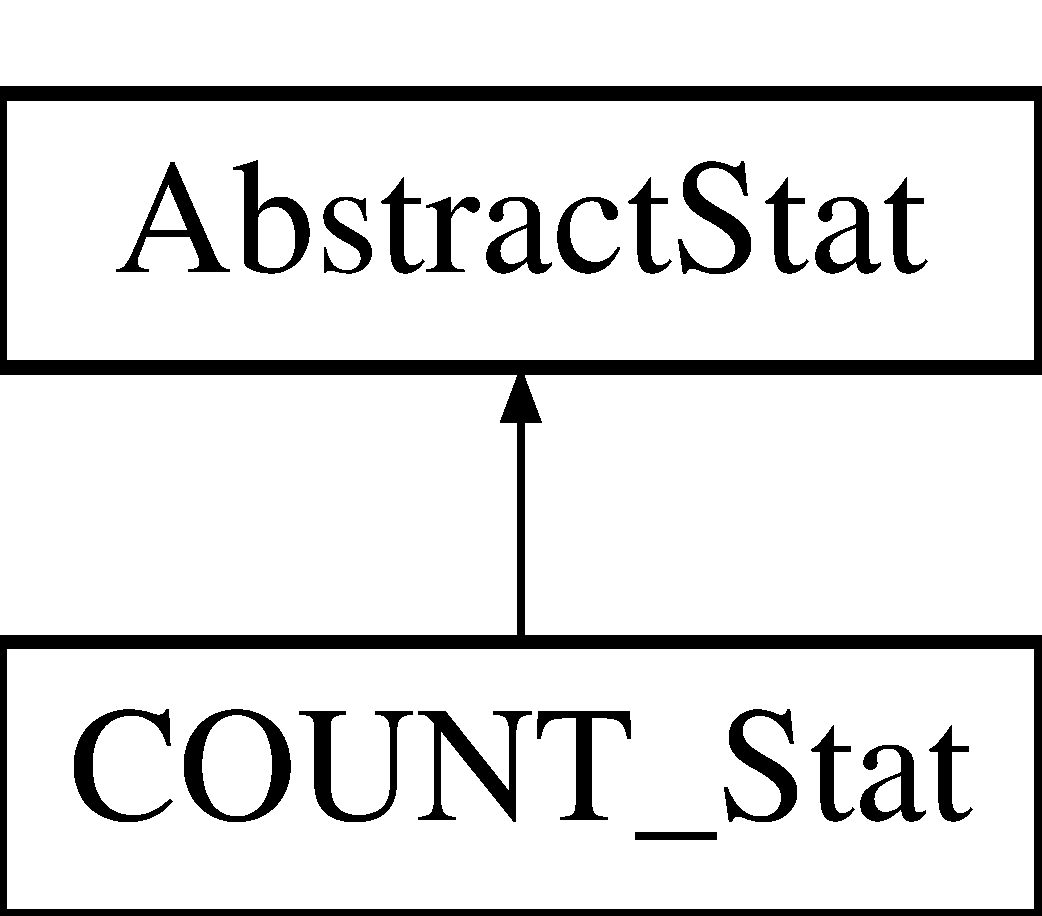
\includegraphics[height=2.000000cm]{classCOUNT__Stat}
\end{center}
\end{figure}
\subsection*{Public Member Functions}
\begin{DoxyCompactItemize}
\item 
\hyperlink{classCOUNT__Stat_ab306d33117de1ab68ce7307c937f1f29}{COUNT\_\-Stat} (const string \&str, const string \&outputfilename, long ID)
\item 
virtual \hyperlink{classCOUNT__Stat_a080c807a9cf2da4fc1fd7c5ffb233528}{$\sim$COUNT\_\-Stat} ()
\item 
virtual \hyperlink{classAbstractStat}{AbstractStat} $\ast$ \hyperlink{classCOUNT__Stat_ad985ac068e44a565f76f1615b2677022}{clone} (unsigned int coreID)
\end{DoxyCompactItemize}


\subsection{Detailed Description}
COUNT type stats. 

\subsection{Constructor \& Destructor Documentation}
\hypertarget{classCOUNT__Stat_ab306d33117de1ab68ce7307c937f1f29}{
\index{COUNT\_\-Stat@{COUNT\_\-Stat}!COUNT\_\-Stat@{COUNT\_\-Stat}}
\index{COUNT\_\-Stat@{COUNT\_\-Stat}!COUNT_Stat@{COUNT\_\-Stat}}
\subsubsection[{COUNT\_\-Stat}]{\setlength{\rightskip}{0pt plus 5cm}COUNT\_\-Stat::COUNT\_\-Stat (
\begin{DoxyParamCaption}
\item[{const string \&}]{ str, }
\item[{const string \&}]{ outputfilename, }
\item[{long}]{ ID}
\end{DoxyParamCaption}
)\hspace{0.3cm}{\ttfamily  \mbox{[}inline\mbox{]}}}}
\label{classCOUNT__Stat_ab306d33117de1ab68ce7307c937f1f29}
Constructor. \hypertarget{classCOUNT__Stat_a080c807a9cf2da4fc1fd7c5ffb233528}{
\index{COUNT\_\-Stat@{COUNT\_\-Stat}!$\sim$COUNT\_\-Stat@{$\sim$COUNT\_\-Stat}}
\index{$\sim$COUNT\_\-Stat@{$\sim$COUNT\_\-Stat}!COUNT_Stat@{COUNT\_\-Stat}}
\subsubsection[{$\sim$COUNT\_\-Stat}]{\setlength{\rightskip}{0pt plus 5cm}virtual COUNT\_\-Stat::$\sim$COUNT\_\-Stat (
\begin{DoxyParamCaption}
{}
\end{DoxyParamCaption}
)\hspace{0.3cm}{\ttfamily  \mbox{[}inline, virtual\mbox{]}}}}
\label{classCOUNT__Stat_a080c807a9cf2da4fc1fd7c5ffb233528}
Destructor. 

\subsection{Member Function Documentation}
\hypertarget{classCOUNT__Stat_ad985ac068e44a565f76f1615b2677022}{
\index{COUNT\_\-Stat@{COUNT\_\-Stat}!clone@{clone}}
\index{clone@{clone}!COUNT_Stat@{COUNT\_\-Stat}}
\subsubsection[{clone}]{\setlength{\rightskip}{0pt plus 5cm}virtual {\bf AbstractStat}$\ast$ COUNT\_\-Stat::clone (
\begin{DoxyParamCaption}
\item[{unsigned int}]{ coreID}
\end{DoxyParamCaption}
)\hspace{0.3cm}{\ttfamily  \mbox{[}inline, virtual\mbox{]}}}}
\label{classCOUNT__Stat_ad985ac068e44a565f76f1615b2677022}
Clone a stat. 

Implements \hyperlink{classAbstractStat_aed9a458491d92fb2cc3c458990d9fab1}{AbstractStat}.



The documentation for this class was generated from the following file:\begin{DoxyCompactItemize}
\item 
statistics.h\end{DoxyCompactItemize}

\hypertarget{classdc__frfcfs__c}{
\section{dc\_\-frfcfs\_\-c Class Reference}
\label{classdc__frfcfs__c}\index{dc\_\-frfcfs\_\-c@{dc\_\-frfcfs\_\-c}}
}


FR-\/FCFS dram scheduling.  




{\ttfamily \#include $<$dram.h$>$}

Inheritance diagram for dc\_\-frfcfs\_\-c:\begin{figure}[H]
\begin{center}
\leavevmode
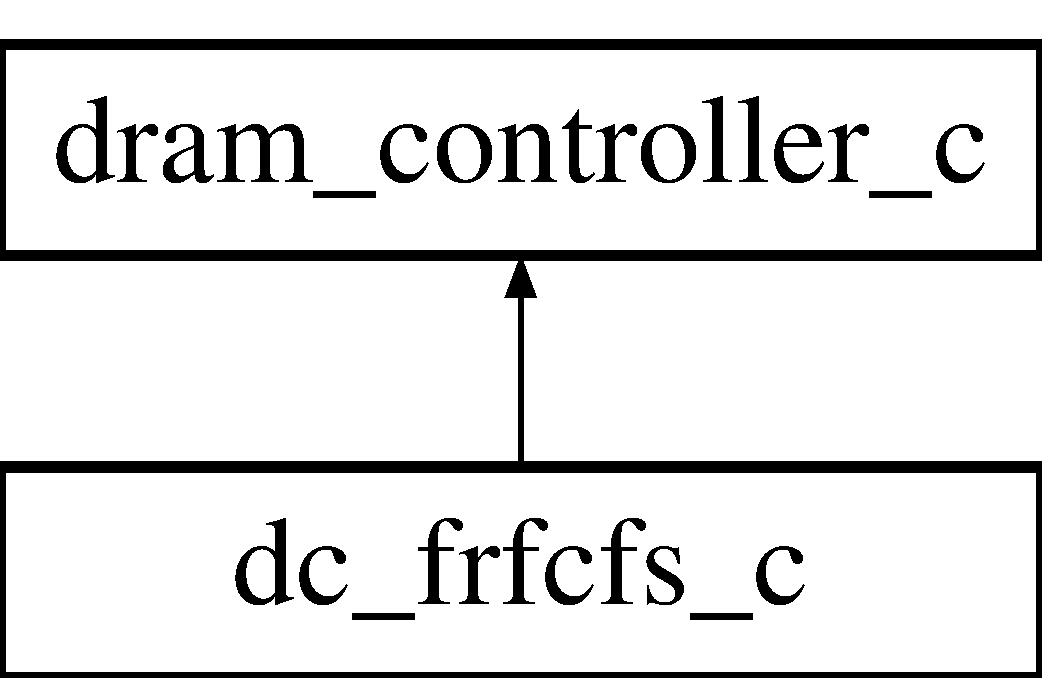
\includegraphics[height=2.000000cm]{classdc__frfcfs__c}
\end{center}
\end{figure}
\subsection*{Classes}
\begin{DoxyCompactItemize}
\item 
class \hyperlink{classdc__frfcfs__c_1_1sort__func}{sort\_\-func}
\begin{DoxyCompactList}\small\item\em \hyperlink{classdc__frfcfs__c}{dc\_\-frfcfs\_\-c} sort function \item\end{DoxyCompactList}\end{DoxyCompactItemize}
\subsection*{Public Member Functions}
\begin{DoxyCompactItemize}
\item 
\hyperlink{classdc__frfcfs__c_ae20cabf0dd64d9d9bac5f5867e73e782}{dc\_\-frfcfs\_\-c} (\hyperlink{classmacsim__c}{macsim\_\-c} $\ast$simBase)
\item 
\hyperlink{classdc__frfcfs__c_a073941102a81c46c76a92b6ecdedc6bd}{$\sim$dc\_\-frfcfs\_\-c} ()
\item 
\hyperlink{structdrb__entry__s}{drb\_\-entry\_\-s} $\ast$ \hyperlink{classdc__frfcfs__c_a4ee4def84ca42d169c13aec01590eeb8}{schedule} (list$<$ \hyperlink{structdrb__entry__s}{drb\_\-entry\_\-s} $\ast$ $>$ $\ast$drb\_\-list)
\end{DoxyCompactItemize}
\subsection*{Private Attributes}
\begin{DoxyCompactItemize}
\item 
class \hyperlink{classdc__frfcfs__c_1_1sort__func}{sort\_\-func} $\ast$ \hyperlink{classdc__frfcfs__c_aea33c4e4bd8214a2331abbbd5a9d59c9}{m\_\-sort}
\end{DoxyCompactItemize}
\subsection*{Friends}
\begin{DoxyCompactItemize}
\item 
\hypertarget{classdc__frfcfs__c_af9acce4ca7c37997aa3dc0c9732ff5e6}{
class {\bfseries sort\_\-func}}
\label{classdc__frfcfs__c_af9acce4ca7c37997aa3dc0c9732ff5e6}

\end{DoxyCompactItemize}


\subsection{Detailed Description}
FR-\/FCFS dram scheduling. 

\subsection{Constructor \& Destructor Documentation}
\hypertarget{classdc__frfcfs__c_ae20cabf0dd64d9d9bac5f5867e73e782}{
\index{dc\_\-frfcfs\_\-c@{dc\_\-frfcfs\_\-c}!dc\_\-frfcfs\_\-c@{dc\_\-frfcfs\_\-c}}
\index{dc\_\-frfcfs\_\-c@{dc\_\-frfcfs\_\-c}!dc_frfcfs_c@{dc\_\-frfcfs\_\-c}}
\subsubsection[{dc\_\-frfcfs\_\-c}]{\setlength{\rightskip}{0pt plus 5cm}dc\_\-frfcfs\_\-c::dc\_\-frfcfs\_\-c (
\begin{DoxyParamCaption}
\item[{{\bf macsim\_\-c} $\ast$}]{ simBase}
\end{DoxyParamCaption}
)}}
\label{classdc__frfcfs__c_ae20cabf0dd64d9d9bac5f5867e73e782}
Constructor \hypertarget{classdc__frfcfs__c_a073941102a81c46c76a92b6ecdedc6bd}{
\index{dc\_\-frfcfs\_\-c@{dc\_\-frfcfs\_\-c}!$\sim$dc\_\-frfcfs\_\-c@{$\sim$dc\_\-frfcfs\_\-c}}
\index{$\sim$dc\_\-frfcfs\_\-c@{$\sim$dc\_\-frfcfs\_\-c}!dc_frfcfs_c@{dc\_\-frfcfs\_\-c}}
\subsubsection[{$\sim$dc\_\-frfcfs\_\-c}]{\setlength{\rightskip}{0pt plus 5cm}dc\_\-frfcfs\_\-c::$\sim$dc\_\-frfcfs\_\-c (
\begin{DoxyParamCaption}
{}
\end{DoxyParamCaption}
)}}
\label{classdc__frfcfs__c_a073941102a81c46c76a92b6ecdedc6bd}
Destructor 

\subsection{Member Function Documentation}
\hypertarget{classdc__frfcfs__c_a4ee4def84ca42d169c13aec01590eeb8}{
\index{dc\_\-frfcfs\_\-c@{dc\_\-frfcfs\_\-c}!schedule@{schedule}}
\index{schedule@{schedule}!dc_frfcfs_c@{dc\_\-frfcfs\_\-c}}
\subsubsection[{schedule}]{\setlength{\rightskip}{0pt plus 5cm}{\bf drb\_\-entry\_\-s} $\ast$ dc\_\-frfcfs\_\-c::schedule (
\begin{DoxyParamCaption}
\item[{list$<$ {\bf drb\_\-entry\_\-s} $\ast$ $>$ $\ast$}]{ drb\_\-list}
\end{DoxyParamCaption}
)\hspace{0.3cm}{\ttfamily  \mbox{[}virtual\mbox{]}}}}
\label{classdc__frfcfs__c_a4ee4def84ca42d169c13aec01590eeb8}
Overloaded schedule function 
\begin{DoxyParams}{Parameters}
\item[{\em drb\_\-list}]-\/ dram request buffer to be scheduled \end{DoxyParams}


Reimplemented from \hyperlink{classdram__controller__c_a0ce04de6742977e7c962ef977c1b9da0}{dram\_\-controller\_\-c}.



\subsection{Member Data Documentation}
\hypertarget{classdc__frfcfs__c_aea33c4e4bd8214a2331abbbd5a9d59c9}{
\index{dc\_\-frfcfs\_\-c@{dc\_\-frfcfs\_\-c}!m\_\-sort@{m\_\-sort}}
\index{m\_\-sort@{m\_\-sort}!dc_frfcfs_c@{dc\_\-frfcfs\_\-c}}
\subsubsection[{m\_\-sort}]{\setlength{\rightskip}{0pt plus 5cm}class {\bf sort\_\-func}$\ast$ {\bf dc\_\-frfcfs\_\-c::m\_\-sort}\hspace{0.3cm}{\ttfamily  \mbox{[}private\mbox{]}}}}
\label{classdc__frfcfs__c_aea33c4e4bd8214a2331abbbd5a9d59c9}
sort function 

The documentation for this class was generated from the following files:\begin{DoxyCompactItemize}
\item 
dram.h\item 
dram.cc\end{DoxyCompactItemize}

\hypertarget{structdcache__data__s}{
\section{dcache\_\-data\_\-s Struct Reference}
\label{structdcache__data__s}\index{dcache\_\-data\_\-s@{dcache\_\-data\_\-s}}
}


data cache data structure  




{\ttfamily \#include $<$memory.h$>$}

\subsection*{Public Attributes}
\begin{DoxyCompactItemize}
\item 
bool \hyperlink{structdcache__data__s_a7cdb5d97e38e3d809bcd15606a1c88cc}{m\_\-dirty}
\item 
Counter \hyperlink{structdcache__data__s_a5314b8ca6633a626c5f4950b4c85098e}{m\_\-fetch\_\-cycle}
\item 
int \hyperlink{structdcache__data__s_a6fec40ec8559ce4500900d904ff7f1be}{m\_\-core\_\-id}
\item 
Addr \hyperlink{structdcache__data__s_a5dfdd969951708a037337450e7ae9f36}{m\_\-pc}
\item 
int \hyperlink{structdcache__data__s_a678d12e44bf2d56cef863426858f62e4}{m\_\-tid}
\end{DoxyCompactItemize}


\subsection{Detailed Description}
data cache data structure 

\subsection{Member Data Documentation}
\hypertarget{structdcache__data__s_a6fec40ec8559ce4500900d904ff7f1be}{
\index{dcache\_\-data\_\-s@{dcache\_\-data\_\-s}!m\_\-core\_\-id@{m\_\-core\_\-id}}
\index{m\_\-core\_\-id@{m\_\-core\_\-id}!dcache_data_s@{dcache\_\-data\_\-s}}
\subsubsection[{m\_\-core\_\-id}]{\setlength{\rightskip}{0pt plus 5cm}int {\bf dcache\_\-data\_\-s::m\_\-core\_\-id}}}
\label{structdcache__data__s_a6fec40ec8559ce4500900d904ff7f1be}
core id \hypertarget{structdcache__data__s_a7cdb5d97e38e3d809bcd15606a1c88cc}{
\index{dcache\_\-data\_\-s@{dcache\_\-data\_\-s}!m\_\-dirty@{m\_\-dirty}}
\index{m\_\-dirty@{m\_\-dirty}!dcache_data_s@{dcache\_\-data\_\-s}}
\subsubsection[{m\_\-dirty}]{\setlength{\rightskip}{0pt plus 5cm}bool {\bf dcache\_\-data\_\-s::m\_\-dirty}}}
\label{structdcache__data__s_a7cdb5d97e38e3d809bcd15606a1c88cc}
line dirty \hypertarget{structdcache__data__s_a5314b8ca6633a626c5f4950b4c85098e}{
\index{dcache\_\-data\_\-s@{dcache\_\-data\_\-s}!m\_\-fetch\_\-cycle@{m\_\-fetch\_\-cycle}}
\index{m\_\-fetch\_\-cycle@{m\_\-fetch\_\-cycle}!dcache_data_s@{dcache\_\-data\_\-s}}
\subsubsection[{m\_\-fetch\_\-cycle}]{\setlength{\rightskip}{0pt plus 5cm}Counter {\bf dcache\_\-data\_\-s::m\_\-fetch\_\-cycle}}}
\label{structdcache__data__s_a5314b8ca6633a626c5f4950b4c85098e}
fetched cycle \hypertarget{structdcache__data__s_a5dfdd969951708a037337450e7ae9f36}{
\index{dcache\_\-data\_\-s@{dcache\_\-data\_\-s}!m\_\-pc@{m\_\-pc}}
\index{m\_\-pc@{m\_\-pc}!dcache_data_s@{dcache\_\-data\_\-s}}
\subsubsection[{m\_\-pc}]{\setlength{\rightskip}{0pt plus 5cm}Addr {\bf dcache\_\-data\_\-s::m\_\-pc}}}
\label{structdcache__data__s_a5dfdd969951708a037337450e7ae9f36}
pc address \hypertarget{structdcache__data__s_a678d12e44bf2d56cef863426858f62e4}{
\index{dcache\_\-data\_\-s@{dcache\_\-data\_\-s}!m\_\-tid@{m\_\-tid}}
\index{m\_\-tid@{m\_\-tid}!dcache_data_s@{dcache\_\-data\_\-s}}
\subsubsection[{m\_\-tid}]{\setlength{\rightskip}{0pt plus 5cm}int {\bf dcache\_\-data\_\-s::m\_\-tid}}}
\label{structdcache__data__s_a678d12e44bf2d56cef863426858f62e4}
thread id 

The documentation for this struct was generated from the following file:\begin{DoxyCompactItemize}
\item 
memory.h\end{DoxyCompactItemize}

\hypertarget{classdcu__c}{
\section{dcu\_\-c Class Reference}
\label{classdcu__c}\index{dcu\_\-c@{dcu\_\-c}}
}


Data cache class.  




{\ttfamily \#include $<$memory.h$>$}

\subsection*{Public Member Functions}
\begin{DoxyCompactItemize}
\item 
\hyperlink{classdcu__c_a84d2ec5db30f22a7aa008351840c2a06}{dcu\_\-c} (int id, Unit\_\-Type type, int level, \hyperlink{classmemory__c}{memory\_\-c} $\ast$mem, int, \hyperlink{classdcu__c}{dcu\_\-c} $\ast$$\ast$next, \hyperlink{classdcu__c}{dcu\_\-c} $\ast$$\ast$prev, \hyperlink{classmacsim__c}{macsim\_\-c} $\ast$simBase)
\item 
\hyperlink{classdcu__c_abea9e7fc68c881ce476cfac7ea891b38}{$\sim$dcu\_\-c} ()
\item 
void \hyperlink{classdcu__c_ae9bcbaf9b038e512463c0879b9e42908}{init} (int next\_\-id, int prev\_\-id, bool done, bool coupled\_\-up, bool coupled\_\-down, bool disable, bool has\_\-router)
\item 
Addr \hyperlink{classdcu__c_a72fb58ab8c0ec711dd31e092e51868a1}{base\_\-addr} (Addr addr)
\item 
int \hyperlink{classdcu__c_a71826360b5e10085fdc427c1f3343b2b}{line\_\-size} ()
\item 
int \hyperlink{classdcu__c_a1fbf4dc5547edff38eb6806294563d91}{bank\_\-id} (Addr addr)
\item 
bool \hyperlink{classdcu__c_a4f712cf333d79a702e40d83935151e29}{get\_\-read\_\-port} (int bank\_\-id)
\item 
int \hyperlink{classdcu__c_a1bfcfc18396925fd9665f6946e73a065}{access} (\hyperlink{classuop__c}{uop\_\-c} $\ast$uop)
\item 
bool \hyperlink{classdcu__c_ad0550e80ffac6ce3078502864f740d5b}{fill} (\hyperlink{structmem__req__s}{mem\_\-req\_\-s} $\ast$req)
\item 
bool \hyperlink{classdcu__c_a5f10df3e409da7fe249aa8c6d87ac6cf}{done} (\hyperlink{structmem__req__s}{mem\_\-req\_\-s} $\ast$req)
\item 
bool \hyperlink{classdcu__c_a215d1e1c6099c6dda22c0cf12b6bd7a4}{insert} (\hyperlink{structmem__req__s}{mem\_\-req\_\-s} $\ast$req)
\item 
void \hyperlink{classdcu__c_a6b4f08e9c538e6d63d0caedecaffdcda}{run\_\-a\_\-cycle} ()
\item 
bool \hyperlink{classdcu__c_aac851f1517b7b10b051491f0ffd09583}{full} ()
\item 
\hyperlink{structdcache__data__s}{dcache\_\-data\_\-s} $\ast$ \hyperlink{classdcu__c_ab04abe7be5561b8cebe2fc5b2b10f677}{access\_\-cache} (Addr addr, Addr $\ast$line\_\-addr, bool update, int appl\_\-id)
\item 
\hyperlink{structmem__req__s}{mem\_\-req\_\-s} $\ast$ \hyperlink{classdcu__c_a44516ada2cdb4e168c71f6b9246e1840}{search\_\-pref\_\-in\_\-queue} ()
\item 
bool \hyperlink{classdcu__c_a64968883497a2f232b3871f7bc05e47e}{create\_\-network\_\-interface} (int)
\item 
bool \hyperlink{classdcu__c_a83778a75013d7c55e929dd86b22e3b25}{send\_\-packet} (\hyperlink{structmem__req__s}{mem\_\-req\_\-s} $\ast$req, int msg, int dir)
\item 
void \hyperlink{classdcu__c_a4ff24d1ebc0e3df58b08d7b8e52af056}{receive\_\-packet} (void)
\end{DoxyCompactItemize}
\subsection*{Private Member Functions}
\begin{DoxyCompactItemize}
\item 
\hyperlink{classdcu__c_ac8bb3b669d6c20b2381f15c7140d4b74}{dcu\_\-c} ()
\item 
void \hyperlink{classdcu__c_a3d18097504fe31cac03406978dd31477}{process\_\-in\_\-queue} ()
\item 
void \hyperlink{classdcu__c_aa34cd13e6faa65115f77d4d01da83096}{process\_\-out\_\-queue} ()
\item 
void \hyperlink{classdcu__c_a8cb64339c417ee62d46298216986e4b5}{process\_\-fill\_\-queue} ()
\item 
void \hyperlink{classdcu__c_aa9c9769a4a8f19bf57365ba1455eb11f}{process\_\-wb\_\-queue} ()
\end{DoxyCompactItemize}
\subsection*{Private Attributes}
\begin{DoxyCompactItemize}
\item 
int \hyperlink{classdcu__c_a61b5178afb8d6af167a3ca3c40aca074}{m\_\-id}
\item 
int \hyperlink{classdcu__c_a3ab8a45d54041c88b9556d2edf07b377}{m\_\-noc\_\-id}
\item 
int \hyperlink{classdcu__c_a04d10c0ce98426f7b14d37c8c60150c0}{m\_\-level}
\item 
bool \hyperlink{classdcu__c_af4dc606e05ca8664ef6a59027d599078}{m\_\-disable}
\item 
bool \hyperlink{classdcu__c_a1991249577b208be4483eeeb98f56295}{m\_\-bypass}
\item 
\hyperlink{classcache__c}{cache\_\-c} $\ast$ \hyperlink{classdcu__c_a6cb56729ba3f6fd05d8071adda723317}{m\_\-cache}
\item 
\hyperlink{classport__c}{port\_\-c} $\ast$$\ast$ \hyperlink{classdcu__c_a6fc4117756ccee0adf08285ad9ef9182}{m\_\-port}
\item 
int \hyperlink{classdcu__c_aaf2ea302ee6c02d0202c0073d12d1813}{m\_\-next\_\-id}
\item 
\hyperlink{classdcu__c}{dcu\_\-c} $\ast$$\ast$ \hyperlink{classdcu__c_a00edf5a77fc43d86790e0a04e7866833}{m\_\-next}
\item 
int \hyperlink{classdcu__c_aab67bf503b09b72441791fc20862c22c}{m\_\-prev\_\-id}
\item 
\hyperlink{classdcu__c}{dcu\_\-c} $\ast$$\ast$ \hyperlink{classdcu__c_a199065735dfd67fbbf17f1e7e73a0b27}{m\_\-prev}
\item 
bool \hyperlink{classdcu__c_aa455e9e2d2d70d9768b01427a5f2ce04}{m\_\-coupled\_\-up}
\item 
bool \hyperlink{classdcu__c_ac252e950738034b9eab0e1774e0e7de5}{m\_\-coupled\_\-down}
\item 
bool \hyperlink{classdcu__c_afd4171d11831e26978f2ce21659b17f8}{m\_\-has\_\-router}
\item 
bool \hyperlink{classdcu__c_aa0f7229cca750799c47e68e4b7025793}{m\_\-done}
\item 
Unit\_\-Type \hyperlink{classdcu__c_ab99a3a4fa14c08b977f91ea53e2d2d8c}{m\_\-type}
\item 
int \hyperlink{classdcu__c_a54ee473e45b0d1a45afe5f569c22d3c1}{m\_\-num\_\-set}
\item 
int \hyperlink{classdcu__c_a8166e3d9828dff8f41078d92767bd920}{m\_\-assoc}
\item 
int \hyperlink{classdcu__c_a54a23275701e0abe535da85c54252ac8}{m\_\-line\_\-size}
\item 
int \hyperlink{classdcu__c_aa1a3af160ffda7483651227049f31185}{m\_\-banks}
\item 
int \hyperlink{classdcu__c_a50a7913d80d0128e9d8926f9104f8e19}{m\_\-latency}
\item 
bool \hyperlink{classdcu__c_a5e56ee48837544fa5f882c9f750fdd43}{m\_\-ptx\_\-sim}
\item 
\hyperlink{classqueue__c}{queue\_\-c} $\ast$ \hyperlink{classdcu__c_a505f2cf05c56380770c1ab1a7f4fb80b}{m\_\-in\_\-queue}
\item 
\hyperlink{classqueue__c}{queue\_\-c} $\ast$ \hyperlink{classdcu__c_a11e746c9849d96d00f6181626d6da7f4}{m\_\-wb\_\-queue}
\item 
\hyperlink{classqueue__c}{queue\_\-c} $\ast$ \hyperlink{classdcu__c_a08eb24546da1c93bfbf88a9c6868930d}{m\_\-fill\_\-queue}
\item 
\hyperlink{classqueue__c}{queue\_\-c} $\ast$ \hyperlink{classdcu__c_a9c0c134e9407debd8308df39c9880e06}{m\_\-out\_\-queue}
\item 
bool \hyperlink{classdcu__c_a9766416e7c7713fe5729a27e6957d80b}{m\_\-req\_\-llc\_\-bypass}
\item 
int \hyperlink{classdcu__c_aa5804689736f9d3db9e5d9a7a88a8b62}{m\_\-num\_\-read\_\-port}
\item 
int \hyperlink{classdcu__c_a490bfb196b859b4f3135368158c4e5e6}{m\_\-num\_\-write\_\-port}
\item 
\hyperlink{classmemory__c}{memory\_\-c} $\ast$ \hyperlink{classdcu__c_a6025ab87f89f05ce3d092aabd941aec6}{m\_\-memory}
\item 
\hyperlink{classmacsim__c}{macsim\_\-c} $\ast$ \hyperlink{classdcu__c_aa9cf359040c048b4163f1961bbff1ca1}{m\_\-simBase}
\item 
ManifoldProcessor $\ast$ \hyperlink{classdcu__c_a3db9363af3f49592efb1edd8014c2736}{m\_\-terminal}
\item 
\hypertarget{classdcu__c_ab55f153fc56152adff3a13457a5405fa}{
\hyperlink{classrouter__c}{router\_\-c} $\ast$ {\bfseries m\_\-router}}
\label{classdcu__c_ab55f153fc56152adff3a13457a5405fa}

\end{DoxyCompactItemize}


\subsection{Detailed Description}
Data cache class. 

\subsection{Constructor \& Destructor Documentation}
\hypertarget{classdcu__c_a84d2ec5db30f22a7aa008351840c2a06}{
\index{dcu\_\-c@{dcu\_\-c}!dcu\_\-c@{dcu\_\-c}}
\index{dcu\_\-c@{dcu\_\-c}!dcu_c@{dcu\_\-c}}
\subsubsection[{dcu\_\-c}]{\setlength{\rightskip}{0pt plus 5cm}dcu\_\-c::dcu\_\-c (
\begin{DoxyParamCaption}
\item[{int}]{ id, }
\item[{Unit\_\-Type}]{ type, }
\item[{int}]{ level, }
\item[{{\bf memory\_\-c} $\ast$}]{ mem, }
\item[{int}]{ noc\_\-id, }
\item[{{\bf dcu\_\-c} $\ast$$\ast$}]{ next, }
\item[{{\bf dcu\_\-c} $\ast$$\ast$}]{ prev, }
\item[{{\bf macsim\_\-c} $\ast$}]{ simBase}
\end{DoxyParamCaption}
)}}
\label{classdcu__c_a84d2ec5db30f22a7aa008351840c2a06}
data cache constructor \hypertarget{classdcu__c_abea9e7fc68c881ce476cfac7ea891b38}{
\index{dcu\_\-c@{dcu\_\-c}!$\sim$dcu\_\-c@{$\sim$dcu\_\-c}}
\index{$\sim$dcu\_\-c@{$\sim$dcu\_\-c}!dcu_c@{dcu\_\-c}}
\subsubsection[{$\sim$dcu\_\-c}]{\setlength{\rightskip}{0pt plus 5cm}dcu\_\-c::$\sim$dcu\_\-c (
\begin{DoxyParamCaption}
{}
\end{DoxyParamCaption}
)}}
\label{classdcu__c_abea9e7fc68c881ce476cfac7ea891b38}
data cache destructor \hypertarget{classdcu__c_ac8bb3b669d6c20b2381f15c7140d4b74}{
\index{dcu\_\-c@{dcu\_\-c}!dcu\_\-c@{dcu\_\-c}}
\index{dcu\_\-c@{dcu\_\-c}!dcu_c@{dcu\_\-c}}
\subsubsection[{dcu\_\-c}]{\setlength{\rightskip}{0pt plus 5cm}dcu\_\-c::dcu\_\-c (
\begin{DoxyParamCaption}
{}
\end{DoxyParamCaption}
)\hspace{0.3cm}{\ttfamily  \mbox{[}private\mbox{]}}}}
\label{classdcu__c_ac8bb3b669d6c20b2381f15c7140d4b74}
data cache default constructor 

\subsection{Member Function Documentation}
\hypertarget{classdcu__c_a1bfcfc18396925fd9665f6946e73a065}{
\index{dcu\_\-c@{dcu\_\-c}!access@{access}}
\index{access@{access}!dcu_c@{dcu\_\-c}}
\subsubsection[{access}]{\setlength{\rightskip}{0pt plus 5cm}int dcu\_\-c::access (
\begin{DoxyParamCaption}
\item[{{\bf uop\_\-c} $\ast$}]{ uop}
\end{DoxyParamCaption}
)}}
\label{classdcu__c_a1bfcfc18396925fd9665f6946e73a065}
Access data cache \hypertarget{classdcu__c_ab04abe7be5561b8cebe2fc5b2b10f677}{
\index{dcu\_\-c@{dcu\_\-c}!access\_\-cache@{access\_\-cache}}
\index{access\_\-cache@{access\_\-cache}!dcu_c@{dcu\_\-c}}
\subsubsection[{access\_\-cache}]{\setlength{\rightskip}{0pt plus 5cm}{\bf dcache\_\-data\_\-s} $\ast$ dcu\_\-c::access\_\-cache (
\begin{DoxyParamCaption}
\item[{Addr}]{ addr, }
\item[{Addr $\ast$}]{ line\_\-addr, }
\item[{bool}]{ update, }
\item[{int}]{ appl\_\-id}
\end{DoxyParamCaption}
)}}
\label{classdcu__c_ab04abe7be5561b8cebe2fc5b2b10f677}
Search a request from queues Access the data cache \hypertarget{classdcu__c_a1fbf4dc5547edff38eb6806294563d91}{
\index{dcu\_\-c@{dcu\_\-c}!bank\_\-id@{bank\_\-id}}
\index{bank\_\-id@{bank\_\-id}!dcu_c@{dcu\_\-c}}
\subsubsection[{bank\_\-id}]{\setlength{\rightskip}{0pt plus 5cm}int dcu\_\-c::bank\_\-id (
\begin{DoxyParamCaption}
\item[{Addr}]{ addr}
\end{DoxyParamCaption}
)}}
\label{classdcu__c_a1fbf4dc5547edff38eb6806294563d91}
Get the bank id \hypertarget{classdcu__c_a72fb58ab8c0ec711dd31e092e51868a1}{
\index{dcu\_\-c@{dcu\_\-c}!base\_\-addr@{base\_\-addr}}
\index{base\_\-addr@{base\_\-addr}!dcu_c@{dcu\_\-c}}
\subsubsection[{base\_\-addr}]{\setlength{\rightskip}{0pt plus 5cm}Addr dcu\_\-c::base\_\-addr (
\begin{DoxyParamCaption}
\item[{Addr}]{ addr}
\end{DoxyParamCaption}
)}}
\label{classdcu__c_a72fb58ab8c0ec711dd31e092e51868a1}
Get the cache line address \hypertarget{classdcu__c_a64968883497a2f232b3871f7bc05e47e}{
\index{dcu\_\-c@{dcu\_\-c}!create\_\-network\_\-interface@{create\_\-network\_\-interface}}
\index{create\_\-network\_\-interface@{create\_\-network\_\-interface}!dcu_c@{dcu\_\-c}}
\subsubsection[{create\_\-network\_\-interface}]{\setlength{\rightskip}{0pt plus 5cm}bool dcu\_\-c::create\_\-network\_\-interface (
\begin{DoxyParamCaption}
\item[{int}]{ mclass}
\end{DoxyParamCaption}
)}}
\label{classdcu__c_a64968883497a2f232b3871f7bc05e47e}
Create the network interface \hypertarget{classdcu__c_a5f10df3e409da7fe249aa8c6d87ac6cf}{
\index{dcu\_\-c@{dcu\_\-c}!done@{done}}
\index{done@{done}!dcu_c@{dcu\_\-c}}
\subsubsection[{done}]{\setlength{\rightskip}{0pt plus 5cm}bool dcu\_\-c::done (
\begin{DoxyParamCaption}
\item[{{\bf mem\_\-req\_\-s} $\ast$}]{ req}
\end{DoxyParamCaption}
)}}
\label{classdcu__c_a5f10df3e409da7fe249aa8c6d87ac6cf}
Fill a cache line \hypertarget{classdcu__c_ad0550e80ffac6ce3078502864f740d5b}{
\index{dcu\_\-c@{dcu\_\-c}!fill@{fill}}
\index{fill@{fill}!dcu_c@{dcu\_\-c}}
\subsubsection[{fill}]{\setlength{\rightskip}{0pt plus 5cm}bool dcu\_\-c::fill (
\begin{DoxyParamCaption}
\item[{{\bf mem\_\-req\_\-s} $\ast$}]{ req}
\end{DoxyParamCaption}
)}}
\label{classdcu__c_ad0550e80ffac6ce3078502864f740d5b}
Insert a request to fill\_\-queue (FILL REQ) \hypertarget{classdcu__c_aac851f1517b7b10b051491f0ffd09583}{
\index{dcu\_\-c@{dcu\_\-c}!full@{full}}
\index{full@{full}!dcu_c@{dcu\_\-c}}
\subsubsection[{full}]{\setlength{\rightskip}{0pt plus 5cm}bool dcu\_\-c::full (
\begin{DoxyParamCaption}
\item[{void}]{}
\end{DoxyParamCaption}
)}}
\label{classdcu__c_aac851f1517b7b10b051491f0ffd09583}
Check available buffer space \hypertarget{classdcu__c_a4f712cf333d79a702e40d83935151e29}{
\index{dcu\_\-c@{dcu\_\-c}!get\_\-read\_\-port@{get\_\-read\_\-port}}
\index{get\_\-read\_\-port@{get\_\-read\_\-port}!dcu_c@{dcu\_\-c}}
\subsubsection[{get\_\-read\_\-port}]{\setlength{\rightskip}{0pt plus 5cm}bool dcu\_\-c::get\_\-read\_\-port (
\begin{DoxyParamCaption}
\item[{int}]{ bank\_\-id}
\end{DoxyParamCaption}
)}}
\label{classdcu__c_a4f712cf333d79a702e40d83935151e29}
Acquire data cache read port \hypertarget{classdcu__c_ae9bcbaf9b038e512463c0879b9e42908}{
\index{dcu\_\-c@{dcu\_\-c}!init@{init}}
\index{init@{init}!dcu_c@{dcu\_\-c}}
\subsubsection[{init}]{\setlength{\rightskip}{0pt plus 5cm}void dcu\_\-c::init (
\begin{DoxyParamCaption}
\item[{int}]{ next\_\-id, }
\item[{int}]{ prev\_\-id, }
\item[{bool}]{ done, }
\item[{bool}]{ coupled\_\-up, }
\item[{bool}]{ coupled\_\-down, }
\item[{bool}]{ disable, }
\item[{bool}]{ has\_\-router}
\end{DoxyParamCaption}
)}}
\label{classdcu__c_ae9bcbaf9b038e512463c0879b9e42908}
Initialize a data cache 
\begin{DoxyParams}{Parameters}
\item[{\em next\_\-id}]next-\/level cache id \item[{\em prev\_\-id}]prev-\/level cache id \item[{\em done}]decide whether corresponding done\_\-func is callable \item[{\em coupled\_\-up}]connected to upper-\/level cache \item[{\em coupled\_\-down}]connected to lower-\/level cache \item[{\em disable}]disabled cache (in case of 2-\/level cache hierarchy) \item[{\em has\_\-router}]decide the next destination (NoC or next cache) \end{DoxyParams}
\hypertarget{classdcu__c_a215d1e1c6099c6dda22c0cf12b6bd7a4}{
\index{dcu\_\-c@{dcu\_\-c}!insert@{insert}}
\index{insert@{insert}!dcu_c@{dcu\_\-c}}
\subsubsection[{insert}]{\setlength{\rightskip}{0pt plus 5cm}bool dcu\_\-c::insert (
\begin{DoxyParamCaption}
\item[{{\bf mem\_\-req\_\-s} $\ast$}]{ req}
\end{DoxyParamCaption}
)}}
\label{classdcu__c_a215d1e1c6099c6dda22c0cf12b6bd7a4}
Insert a request to in\_\-queue (NEW REQ) \hypertarget{classdcu__c_a71826360b5e10085fdc427c1f3343b2b}{
\index{dcu\_\-c@{dcu\_\-c}!line\_\-size@{line\_\-size}}
\index{line\_\-size@{line\_\-size}!dcu_c@{dcu\_\-c}}
\subsubsection[{line\_\-size}]{\setlength{\rightskip}{0pt plus 5cm}int dcu\_\-c::line\_\-size (
\begin{DoxyParamCaption}
{}
\end{DoxyParamCaption}
)}}
\label{classdcu__c_a71826360b5e10085fdc427c1f3343b2b}
Get the cache line size \hypertarget{classdcu__c_a8cb64339c417ee62d46298216986e4b5}{
\index{dcu\_\-c@{dcu\_\-c}!process\_\-fill\_\-queue@{process\_\-fill\_\-queue}}
\index{process\_\-fill\_\-queue@{process\_\-fill\_\-queue}!dcu_c@{dcu\_\-c}}
\subsubsection[{process\_\-fill\_\-queue}]{\setlength{\rightskip}{0pt plus 5cm}void dcu\_\-c::process\_\-fill\_\-queue (
\begin{DoxyParamCaption}
{}
\end{DoxyParamCaption}
)\hspace{0.3cm}{\ttfamily  \mbox{[}private\mbox{]}}}}
\label{classdcu__c_a8cb64339c417ee62d46298216986e4b5}
Process requests from fill\_\-queue \hypertarget{classdcu__c_a3d18097504fe31cac03406978dd31477}{
\index{dcu\_\-c@{dcu\_\-c}!process\_\-in\_\-queue@{process\_\-in\_\-queue}}
\index{process\_\-in\_\-queue@{process\_\-in\_\-queue}!dcu_c@{dcu\_\-c}}
\subsubsection[{process\_\-in\_\-queue}]{\setlength{\rightskip}{0pt plus 5cm}void dcu\_\-c::process\_\-in\_\-queue (
\begin{DoxyParamCaption}
{}
\end{DoxyParamCaption}
)\hspace{0.3cm}{\ttfamily  \mbox{[}private\mbox{]}}}}
\label{classdcu__c_a3d18097504fe31cac03406978dd31477}
Process requests from in\_\-queue \hypertarget{classdcu__c_aa34cd13e6faa65115f77d4d01da83096}{
\index{dcu\_\-c@{dcu\_\-c}!process\_\-out\_\-queue@{process\_\-out\_\-queue}}
\index{process\_\-out\_\-queue@{process\_\-out\_\-queue}!dcu_c@{dcu\_\-c}}
\subsubsection[{process\_\-out\_\-queue}]{\setlength{\rightskip}{0pt plus 5cm}void dcu\_\-c::process\_\-out\_\-queue (
\begin{DoxyParamCaption}
{}
\end{DoxyParamCaption}
)\hspace{0.3cm}{\ttfamily  \mbox{[}private\mbox{]}}}}
\label{classdcu__c_aa34cd13e6faa65115f77d4d01da83096}
Process requests from out\_\-queue \hypertarget{classdcu__c_aa9c9769a4a8f19bf57365ba1455eb11f}{
\index{dcu\_\-c@{dcu\_\-c}!process\_\-wb\_\-queue@{process\_\-wb\_\-queue}}
\index{process\_\-wb\_\-queue@{process\_\-wb\_\-queue}!dcu_c@{dcu\_\-c}}
\subsubsection[{process\_\-wb\_\-queue}]{\setlength{\rightskip}{0pt plus 5cm}void dcu\_\-c::process\_\-wb\_\-queue (
\begin{DoxyParamCaption}
{}
\end{DoxyParamCaption}
)\hspace{0.3cm}{\ttfamily  \mbox{[}private\mbox{]}}}}
\label{classdcu__c_aa9c9769a4a8f19bf57365ba1455eb11f}
Process requests from wb\_\-queue \hypertarget{classdcu__c_a4ff24d1ebc0e3df58b08d7b8e52af056}{
\index{dcu\_\-c@{dcu\_\-c}!receive\_\-packet@{receive\_\-packet}}
\index{receive\_\-packet@{receive\_\-packet}!dcu_c@{dcu\_\-c}}
\subsubsection[{receive\_\-packet}]{\setlength{\rightskip}{0pt plus 5cm}void dcu\_\-c::receive\_\-packet (
\begin{DoxyParamCaption}
\item[{void}]{}
\end{DoxyParamCaption}
)}}
\label{classdcu__c_a4ff24d1ebc0e3df58b08d7b8e52af056}
Receive a packet from the NoC \hypertarget{classdcu__c_a6b4f08e9c538e6d63d0caedecaffdcda}{
\index{dcu\_\-c@{dcu\_\-c}!run\_\-a\_\-cycle@{run\_\-a\_\-cycle}}
\index{run\_\-a\_\-cycle@{run\_\-a\_\-cycle}!dcu_c@{dcu\_\-c}}
\subsubsection[{run\_\-a\_\-cycle}]{\setlength{\rightskip}{0pt plus 5cm}void dcu\_\-c::run\_\-a\_\-cycle (
\begin{DoxyParamCaption}
\item[{void}]{}
\end{DoxyParamCaption}
)}}
\label{classdcu__c_a6b4f08e9c538e6d63d0caedecaffdcda}
Tick a cycle \hypertarget{classdcu__c_a44516ada2cdb4e168c71f6b9246e1840}{
\index{dcu\_\-c@{dcu\_\-c}!search\_\-pref\_\-in\_\-queue@{search\_\-pref\_\-in\_\-queue}}
\index{search\_\-pref\_\-in\_\-queue@{search\_\-pref\_\-in\_\-queue}!dcu_c@{dcu\_\-c}}
\subsubsection[{search\_\-pref\_\-in\_\-queue}]{\setlength{\rightskip}{0pt plus 5cm}{\bf mem\_\-req\_\-s} $\ast$ dcu\_\-c::search\_\-pref\_\-in\_\-queue (
\begin{DoxyParamCaption}
{}
\end{DoxyParamCaption}
)}}
\label{classdcu__c_a44516ada2cdb4e168c71f6b9246e1840}
Search a prefetch request from queues \hypertarget{classdcu__c_a83778a75013d7c55e929dd86b22e3b25}{
\index{dcu\_\-c@{dcu\_\-c}!send\_\-packet@{send\_\-packet}}
\index{send\_\-packet@{send\_\-packet}!dcu_c@{dcu\_\-c}}
\subsubsection[{send\_\-packet}]{\setlength{\rightskip}{0pt plus 5cm}bool dcu\_\-c::send\_\-packet (
\begin{DoxyParamCaption}
\item[{{\bf mem\_\-req\_\-s} $\ast$}]{ req, }
\item[{int}]{ msg, }
\item[{int}]{ dir}
\end{DoxyParamCaption}
)}}
\label{classdcu__c_a83778a75013d7c55e929dd86b22e3b25}
Send a packet to the NoC 
\begin{DoxyParams}{Parameters}
\item[{\em req}]-\/ memory request to be sent \item[{\em msg}]-\/ message type \item[{\em dir}]-\/ direction \end{DoxyParams}


\subsection{Member Data Documentation}
\hypertarget{classdcu__c_a8166e3d9828dff8f41078d92767bd920}{
\index{dcu\_\-c@{dcu\_\-c}!m\_\-assoc@{m\_\-assoc}}
\index{m\_\-assoc@{m\_\-assoc}!dcu_c@{dcu\_\-c}}
\subsubsection[{m\_\-assoc}]{\setlength{\rightskip}{0pt plus 5cm}int {\bf dcu\_\-c::m\_\-assoc}\hspace{0.3cm}{\ttfamily  \mbox{[}private\mbox{]}}}}
\label{classdcu__c_a8166e3d9828dff8f41078d92767bd920}
cache associativity \hypertarget{classdcu__c_aa1a3af160ffda7483651227049f31185}{
\index{dcu\_\-c@{dcu\_\-c}!m\_\-banks@{m\_\-banks}}
\index{m\_\-banks@{m\_\-banks}!dcu_c@{dcu\_\-c}}
\subsubsection[{m\_\-banks}]{\setlength{\rightskip}{0pt plus 5cm}int {\bf dcu\_\-c::m\_\-banks}\hspace{0.3cm}{\ttfamily  \mbox{[}private\mbox{]}}}}
\label{classdcu__c_aa1a3af160ffda7483651227049f31185}
number of cache banks \hypertarget{classdcu__c_a1991249577b208be4483eeeb98f56295}{
\index{dcu\_\-c@{dcu\_\-c}!m\_\-bypass@{m\_\-bypass}}
\index{m\_\-bypass@{m\_\-bypass}!dcu_c@{dcu\_\-c}}
\subsubsection[{m\_\-bypass}]{\setlength{\rightskip}{0pt plus 5cm}bool {\bf dcu\_\-c::m\_\-bypass}\hspace{0.3cm}{\ttfamily  \mbox{[}private\mbox{]}}}}
\label{classdcu__c_a1991249577b208be4483eeeb98f56295}
bypass cache \hypertarget{classdcu__c_a6cb56729ba3f6fd05d8071adda723317}{
\index{dcu\_\-c@{dcu\_\-c}!m\_\-cache@{m\_\-cache}}
\index{m\_\-cache@{m\_\-cache}!dcu_c@{dcu\_\-c}}
\subsubsection[{m\_\-cache}]{\setlength{\rightskip}{0pt plus 5cm}{\bf cache\_\-c}$\ast$ {\bf dcu\_\-c::m\_\-cache}\hspace{0.3cm}{\ttfamily  \mbox{[}private\mbox{]}}}}
\label{classdcu__c_a6cb56729ba3f6fd05d8071adda723317}
cache structure \hypertarget{classdcu__c_ac252e950738034b9eab0e1774e0e7de5}{
\index{dcu\_\-c@{dcu\_\-c}!m\_\-coupled\_\-down@{m\_\-coupled\_\-down}}
\index{m\_\-coupled\_\-down@{m\_\-coupled\_\-down}!dcu_c@{dcu\_\-c}}
\subsubsection[{m\_\-coupled\_\-down}]{\setlength{\rightskip}{0pt plus 5cm}bool {\bf dcu\_\-c::m\_\-coupled\_\-down}\hspace{0.3cm}{\ttfamily  \mbox{[}private\mbox{]}}}}
\label{classdcu__c_ac252e950738034b9eab0e1774e0e7de5}
directly connected to downward cache w/o NoC \hypertarget{classdcu__c_aa455e9e2d2d70d9768b01427a5f2ce04}{
\index{dcu\_\-c@{dcu\_\-c}!m\_\-coupled\_\-up@{m\_\-coupled\_\-up}}
\index{m\_\-coupled\_\-up@{m\_\-coupled\_\-up}!dcu_c@{dcu\_\-c}}
\subsubsection[{m\_\-coupled\_\-up}]{\setlength{\rightskip}{0pt plus 5cm}bool {\bf dcu\_\-c::m\_\-coupled\_\-up}\hspace{0.3cm}{\ttfamily  \mbox{[}private\mbox{]}}}}
\label{classdcu__c_aa455e9e2d2d70d9768b01427a5f2ce04}
directly connected to upward cache w/o NoC \hypertarget{classdcu__c_af4dc606e05ca8664ef6a59027d599078}{
\index{dcu\_\-c@{dcu\_\-c}!m\_\-disable@{m\_\-disable}}
\index{m\_\-disable@{m\_\-disable}!dcu_c@{dcu\_\-c}}
\subsubsection[{m\_\-disable}]{\setlength{\rightskip}{0pt plus 5cm}bool {\bf dcu\_\-c::m\_\-disable}\hspace{0.3cm}{\ttfamily  \mbox{[}private\mbox{]}}}}
\label{classdcu__c_af4dc606e05ca8664ef6a59027d599078}
disabled \hypertarget{classdcu__c_aa0f7229cca750799c47e68e4b7025793}{
\index{dcu\_\-c@{dcu\_\-c}!m\_\-done@{m\_\-done}}
\index{m\_\-done@{m\_\-done}!dcu_c@{dcu\_\-c}}
\subsubsection[{m\_\-done}]{\setlength{\rightskip}{0pt plus 5cm}bool {\bf dcu\_\-c::m\_\-done}\hspace{0.3cm}{\ttfamily  \mbox{[}private\mbox{]}}}}
\label{classdcu__c_aa0f7229cca750799c47e68e4b7025793}
done\_\-func can be called \hypertarget{classdcu__c_a08eb24546da1c93bfbf88a9c6868930d}{
\index{dcu\_\-c@{dcu\_\-c}!m\_\-fill\_\-queue@{m\_\-fill\_\-queue}}
\index{m\_\-fill\_\-queue@{m\_\-fill\_\-queue}!dcu_c@{dcu\_\-c}}
\subsubsection[{m\_\-fill\_\-queue}]{\setlength{\rightskip}{0pt plus 5cm}{\bf queue\_\-c}$\ast$ {\bf dcu\_\-c::m\_\-fill\_\-queue}\hspace{0.3cm}{\ttfamily  \mbox{[}private\mbox{]}}}}
\label{classdcu__c_a08eb24546da1c93bfbf88a9c6868930d}
fill queue \hypertarget{classdcu__c_afd4171d11831e26978f2ce21659b17f8}{
\index{dcu\_\-c@{dcu\_\-c}!m\_\-has\_\-router@{m\_\-has\_\-router}}
\index{m\_\-has\_\-router@{m\_\-has\_\-router}!dcu_c@{dcu\_\-c}}
\subsubsection[{m\_\-has\_\-router}]{\setlength{\rightskip}{0pt plus 5cm}bool {\bf dcu\_\-c::m\_\-has\_\-router}\hspace{0.3cm}{\ttfamily  \mbox{[}private\mbox{]}}}}
\label{classdcu__c_afd4171d11831e26978f2ce21659b17f8}
has network router in this level \hypertarget{classdcu__c_a61b5178afb8d6af167a3ca3c40aca074}{
\index{dcu\_\-c@{dcu\_\-c}!m\_\-id@{m\_\-id}}
\index{m\_\-id@{m\_\-id}!dcu_c@{dcu\_\-c}}
\subsubsection[{m\_\-id}]{\setlength{\rightskip}{0pt plus 5cm}int {\bf dcu\_\-c::m\_\-id}\hspace{0.3cm}{\ttfamily  \mbox{[}private\mbox{]}}}}
\label{classdcu__c_a61b5178afb8d6af167a3ca3c40aca074}
cache id \hypertarget{classdcu__c_a505f2cf05c56380770c1ab1a7f4fb80b}{
\index{dcu\_\-c@{dcu\_\-c}!m\_\-in\_\-queue@{m\_\-in\_\-queue}}
\index{m\_\-in\_\-queue@{m\_\-in\_\-queue}!dcu_c@{dcu\_\-c}}
\subsubsection[{m\_\-in\_\-queue}]{\setlength{\rightskip}{0pt plus 5cm}{\bf queue\_\-c}$\ast$ {\bf dcu\_\-c::m\_\-in\_\-queue}\hspace{0.3cm}{\ttfamily  \mbox{[}private\mbox{]}}}}
\label{classdcu__c_a505f2cf05c56380770c1ab1a7f4fb80b}
input queue \hypertarget{classdcu__c_a50a7913d80d0128e9d8926f9104f8e19}{
\index{dcu\_\-c@{dcu\_\-c}!m\_\-latency@{m\_\-latency}}
\index{m\_\-latency@{m\_\-latency}!dcu_c@{dcu\_\-c}}
\subsubsection[{m\_\-latency}]{\setlength{\rightskip}{0pt plus 5cm}int {\bf dcu\_\-c::m\_\-latency}\hspace{0.3cm}{\ttfamily  \mbox{[}private\mbox{]}}}}
\label{classdcu__c_a50a7913d80d0128e9d8926f9104f8e19}
cache access latency \hypertarget{classdcu__c_a04d10c0ce98426f7b14d37c8c60150c0}{
\index{dcu\_\-c@{dcu\_\-c}!m\_\-level@{m\_\-level}}
\index{m\_\-level@{m\_\-level}!dcu_c@{dcu\_\-c}}
\subsubsection[{m\_\-level}]{\setlength{\rightskip}{0pt plus 5cm}int {\bf dcu\_\-c::m\_\-level}\hspace{0.3cm}{\ttfamily  \mbox{[}private\mbox{]}}}}
\label{classdcu__c_a04d10c0ce98426f7b14d37c8c60150c0}
cache level (L1, L2, L3, or memory controller) \hypertarget{classdcu__c_a54a23275701e0abe535da85c54252ac8}{
\index{dcu\_\-c@{dcu\_\-c}!m\_\-line\_\-size@{m\_\-line\_\-size}}
\index{m\_\-line\_\-size@{m\_\-line\_\-size}!dcu_c@{dcu\_\-c}}
\subsubsection[{m\_\-line\_\-size}]{\setlength{\rightskip}{0pt plus 5cm}int {\bf dcu\_\-c::m\_\-line\_\-size}\hspace{0.3cm}{\ttfamily  \mbox{[}private\mbox{]}}}}
\label{classdcu__c_a54a23275701e0abe535da85c54252ac8}
cache line size \hypertarget{classdcu__c_a6025ab87f89f05ce3d092aabd941aec6}{
\index{dcu\_\-c@{dcu\_\-c}!m\_\-memory@{m\_\-memory}}
\index{m\_\-memory@{m\_\-memory}!dcu_c@{dcu\_\-c}}
\subsubsection[{m\_\-memory}]{\setlength{\rightskip}{0pt plus 5cm}{\bf memory\_\-c}$\ast$ {\bf dcu\_\-c::m\_\-memory}\hspace{0.3cm}{\ttfamily  \mbox{[}private\mbox{]}}}}
\label{classdcu__c_a6025ab87f89f05ce3d092aabd941aec6}
pointer to the memory system \hypertarget{classdcu__c_a00edf5a77fc43d86790e0a04e7866833}{
\index{dcu\_\-c@{dcu\_\-c}!m\_\-next@{m\_\-next}}
\index{m\_\-next@{m\_\-next}!dcu_c@{dcu\_\-c}}
\subsubsection[{m\_\-next}]{\setlength{\rightskip}{0pt plus 5cm}{\bf dcu\_\-c}$\ast$$\ast$ {\bf dcu\_\-c::m\_\-next}\hspace{0.3cm}{\ttfamily  \mbox{[}private\mbox{]}}}}
\label{classdcu__c_a00edf5a77fc43d86790e0a04e7866833}
next-\/level cache pointer \hypertarget{classdcu__c_aaf2ea302ee6c02d0202c0073d12d1813}{
\index{dcu\_\-c@{dcu\_\-c}!m\_\-next\_\-id@{m\_\-next\_\-id}}
\index{m\_\-next\_\-id@{m\_\-next\_\-id}!dcu_c@{dcu\_\-c}}
\subsubsection[{m\_\-next\_\-id}]{\setlength{\rightskip}{0pt plus 5cm}int {\bf dcu\_\-c::m\_\-next\_\-id}\hspace{0.3cm}{\ttfamily  \mbox{[}private\mbox{]}}}}
\label{classdcu__c_aaf2ea302ee6c02d0202c0073d12d1813}
next-\/level cache id \hypertarget{classdcu__c_a3ab8a45d54041c88b9556d2edf07b377}{
\index{dcu\_\-c@{dcu\_\-c}!m\_\-noc\_\-id@{m\_\-noc\_\-id}}
\index{m\_\-noc\_\-id@{m\_\-noc\_\-id}!dcu_c@{dcu\_\-c}}
\subsubsection[{m\_\-noc\_\-id}]{\setlength{\rightskip}{0pt plus 5cm}int {\bf dcu\_\-c::m\_\-noc\_\-id}\hspace{0.3cm}{\ttfamily  \mbox{[}private\mbox{]}}}}
\label{classdcu__c_a3ab8a45d54041c88b9556d2edf07b377}
cache network id \hypertarget{classdcu__c_aa5804689736f9d3db9e5d9a7a88a8b62}{
\index{dcu\_\-c@{dcu\_\-c}!m\_\-num\_\-read\_\-port@{m\_\-num\_\-read\_\-port}}
\index{m\_\-num\_\-read\_\-port@{m\_\-num\_\-read\_\-port}!dcu_c@{dcu\_\-c}}
\subsubsection[{m\_\-num\_\-read\_\-port}]{\setlength{\rightskip}{0pt plus 5cm}int {\bf dcu\_\-c::m\_\-num\_\-read\_\-port}\hspace{0.3cm}{\ttfamily  \mbox{[}private\mbox{]}}}}
\label{classdcu__c_aa5804689736f9d3db9e5d9a7a88a8b62}
number of read ports \hypertarget{classdcu__c_a54ee473e45b0d1a45afe5f569c22d3c1}{
\index{dcu\_\-c@{dcu\_\-c}!m\_\-num\_\-set@{m\_\-num\_\-set}}
\index{m\_\-num\_\-set@{m\_\-num\_\-set}!dcu_c@{dcu\_\-c}}
\subsubsection[{m\_\-num\_\-set}]{\setlength{\rightskip}{0pt plus 5cm}int {\bf dcu\_\-c::m\_\-num\_\-set}\hspace{0.3cm}{\ttfamily  \mbox{[}private\mbox{]}}}}
\label{classdcu__c_a54ee473e45b0d1a45afe5f569c22d3c1}
number of cache sets \hypertarget{classdcu__c_a490bfb196b859b4f3135368158c4e5e6}{
\index{dcu\_\-c@{dcu\_\-c}!m\_\-num\_\-write\_\-port@{m\_\-num\_\-write\_\-port}}
\index{m\_\-num\_\-write\_\-port@{m\_\-num\_\-write\_\-port}!dcu_c@{dcu\_\-c}}
\subsubsection[{m\_\-num\_\-write\_\-port}]{\setlength{\rightskip}{0pt plus 5cm}int {\bf dcu\_\-c::m\_\-num\_\-write\_\-port}\hspace{0.3cm}{\ttfamily  \mbox{[}private\mbox{]}}}}
\label{classdcu__c_a490bfb196b859b4f3135368158c4e5e6}
number of write ports \hypertarget{classdcu__c_a9c0c134e9407debd8308df39c9880e06}{
\index{dcu\_\-c@{dcu\_\-c}!m\_\-out\_\-queue@{m\_\-out\_\-queue}}
\index{m\_\-out\_\-queue@{m\_\-out\_\-queue}!dcu_c@{dcu\_\-c}}
\subsubsection[{m\_\-out\_\-queue}]{\setlength{\rightskip}{0pt plus 5cm}{\bf queue\_\-c}$\ast$ {\bf dcu\_\-c::m\_\-out\_\-queue}\hspace{0.3cm}{\ttfamily  \mbox{[}private\mbox{]}}}}
\label{classdcu__c_a9c0c134e9407debd8308df39c9880e06}
out queue \hypertarget{classdcu__c_a6fc4117756ccee0adf08285ad9ef9182}{
\index{dcu\_\-c@{dcu\_\-c}!m\_\-port@{m\_\-port}}
\index{m\_\-port@{m\_\-port}!dcu_c@{dcu\_\-c}}
\subsubsection[{m\_\-port}]{\setlength{\rightskip}{0pt plus 5cm}{\bf port\_\-c}$\ast$$\ast$ {\bf dcu\_\-c::m\_\-port}\hspace{0.3cm}{\ttfamily  \mbox{[}private\mbox{]}}}}
\label{classdcu__c_a6fc4117756ccee0adf08285ad9ef9182}
cache port \hypertarget{classdcu__c_a199065735dfd67fbbf17f1e7e73a0b27}{
\index{dcu\_\-c@{dcu\_\-c}!m\_\-prev@{m\_\-prev}}
\index{m\_\-prev@{m\_\-prev}!dcu_c@{dcu\_\-c}}
\subsubsection[{m\_\-prev}]{\setlength{\rightskip}{0pt plus 5cm}{\bf dcu\_\-c}$\ast$$\ast$ {\bf dcu\_\-c::m\_\-prev}\hspace{0.3cm}{\ttfamily  \mbox{[}private\mbox{]}}}}
\label{classdcu__c_a199065735dfd67fbbf17f1e7e73a0b27}
previous-\/level ache pointer \hypertarget{classdcu__c_aab67bf503b09b72441791fc20862c22c}{
\index{dcu\_\-c@{dcu\_\-c}!m\_\-prev\_\-id@{m\_\-prev\_\-id}}
\index{m\_\-prev\_\-id@{m\_\-prev\_\-id}!dcu_c@{dcu\_\-c}}
\subsubsection[{m\_\-prev\_\-id}]{\setlength{\rightskip}{0pt plus 5cm}int {\bf dcu\_\-c::m\_\-prev\_\-id}\hspace{0.3cm}{\ttfamily  \mbox{[}private\mbox{]}}}}
\label{classdcu__c_aab67bf503b09b72441791fc20862c22c}
previous-\/level cache id \hypertarget{classdcu__c_a5e56ee48837544fa5f882c9f750fdd43}{
\index{dcu\_\-c@{dcu\_\-c}!m\_\-ptx\_\-sim@{m\_\-ptx\_\-sim}}
\index{m\_\-ptx\_\-sim@{m\_\-ptx\_\-sim}!dcu_c@{dcu\_\-c}}
\subsubsection[{m\_\-ptx\_\-sim}]{\setlength{\rightskip}{0pt plus 5cm}bool {\bf dcu\_\-c::m\_\-ptx\_\-sim}\hspace{0.3cm}{\ttfamily  \mbox{[}private\mbox{]}}}}
\label{classdcu__c_a5e56ee48837544fa5f882c9f750fdd43}
gpu cache \hypertarget{classdcu__c_a9766416e7c7713fe5729a27e6957d80b}{
\index{dcu\_\-c@{dcu\_\-c}!m\_\-req\_\-llc\_\-bypass@{m\_\-req\_\-llc\_\-bypass}}
\index{m\_\-req\_\-llc\_\-bypass@{m\_\-req\_\-llc\_\-bypass}!dcu_c@{dcu\_\-c}}
\subsubsection[{m\_\-req\_\-llc\_\-bypass}]{\setlength{\rightskip}{0pt plus 5cm}bool {\bf dcu\_\-c::m\_\-req\_\-llc\_\-bypass}\hspace{0.3cm}{\ttfamily  \mbox{[}private\mbox{]}}}}
\label{classdcu__c_a9766416e7c7713fe5729a27e6957d80b}
bypass llc \hypertarget{classdcu__c_aa9cf359040c048b4163f1961bbff1ca1}{
\index{dcu\_\-c@{dcu\_\-c}!m\_\-simBase@{m\_\-simBase}}
\index{m\_\-simBase@{m\_\-simBase}!dcu_c@{dcu\_\-c}}
\subsubsection[{m\_\-simBase}]{\setlength{\rightskip}{0pt plus 5cm}{\bf macsim\_\-c}$\ast$ {\bf dcu\_\-c::m\_\-simBase}\hspace{0.3cm}{\ttfamily  \mbox{[}private\mbox{]}}}}
\label{classdcu__c_aa9cf359040c048b4163f1961bbff1ca1}
\hyperlink{classmacsim__c}{macsim\_\-c} base class for simulation globals \hypertarget{classdcu__c_a3db9363af3f49592efb1edd8014c2736}{
\index{dcu\_\-c@{dcu\_\-c}!m\_\-terminal@{m\_\-terminal}}
\index{m\_\-terminal@{m\_\-terminal}!dcu_c@{dcu\_\-c}}
\subsubsection[{m\_\-terminal}]{\setlength{\rightskip}{0pt plus 5cm}ManifoldProcessor$\ast$ {\bf dcu\_\-c::m\_\-terminal}\hspace{0.3cm}{\ttfamily  \mbox{[}private\mbox{]}}}}
\label{classdcu__c_a3db9363af3f49592efb1edd8014c2736}
terminal to the NoC router \hypertarget{classdcu__c_ab99a3a4fa14c08b977f91ea53e2d2d8c}{
\index{dcu\_\-c@{dcu\_\-c}!m\_\-type@{m\_\-type}}
\index{m\_\-type@{m\_\-type}!dcu_c@{dcu\_\-c}}
\subsubsection[{m\_\-type}]{\setlength{\rightskip}{0pt plus 5cm}Unit\_\-Type {\bf dcu\_\-c::m\_\-type}\hspace{0.3cm}{\ttfamily  \mbox{[}private\mbox{]}}}}
\label{classdcu__c_ab99a3a4fa14c08b977f91ea53e2d2d8c}
core type that this cache belongs to \hypertarget{classdcu__c_a11e746c9849d96d00f6181626d6da7f4}{
\index{dcu\_\-c@{dcu\_\-c}!m\_\-wb\_\-queue@{m\_\-wb\_\-queue}}
\index{m\_\-wb\_\-queue@{m\_\-wb\_\-queue}!dcu_c@{dcu\_\-c}}
\subsubsection[{m\_\-wb\_\-queue}]{\setlength{\rightskip}{0pt plus 5cm}{\bf queue\_\-c}$\ast$ {\bf dcu\_\-c::m\_\-wb\_\-queue}\hspace{0.3cm}{\ttfamily  \mbox{[}private\mbox{]}}}}
\label{classdcu__c_a11e746c9849d96d00f6181626d6da7f4}
write-\/back queue 

The documentation for this class was generated from the following files:\begin{DoxyCompactItemize}
\item 
memory.h\item 
memory.cc\end{DoxyCompactItemize}

\hypertarget{classDIST__Stat}{
\section{DIST\_\-Stat Class Reference}
\label{classDIST__Stat}\index{DIST\_\-Stat@{DIST\_\-Stat}}
}


DIST type stat.  




{\ttfamily \#include $<$statistics.h$>$}

Inheritance diagram for DIST\_\-Stat:\begin{figure}[H]
\begin{center}
\leavevmode
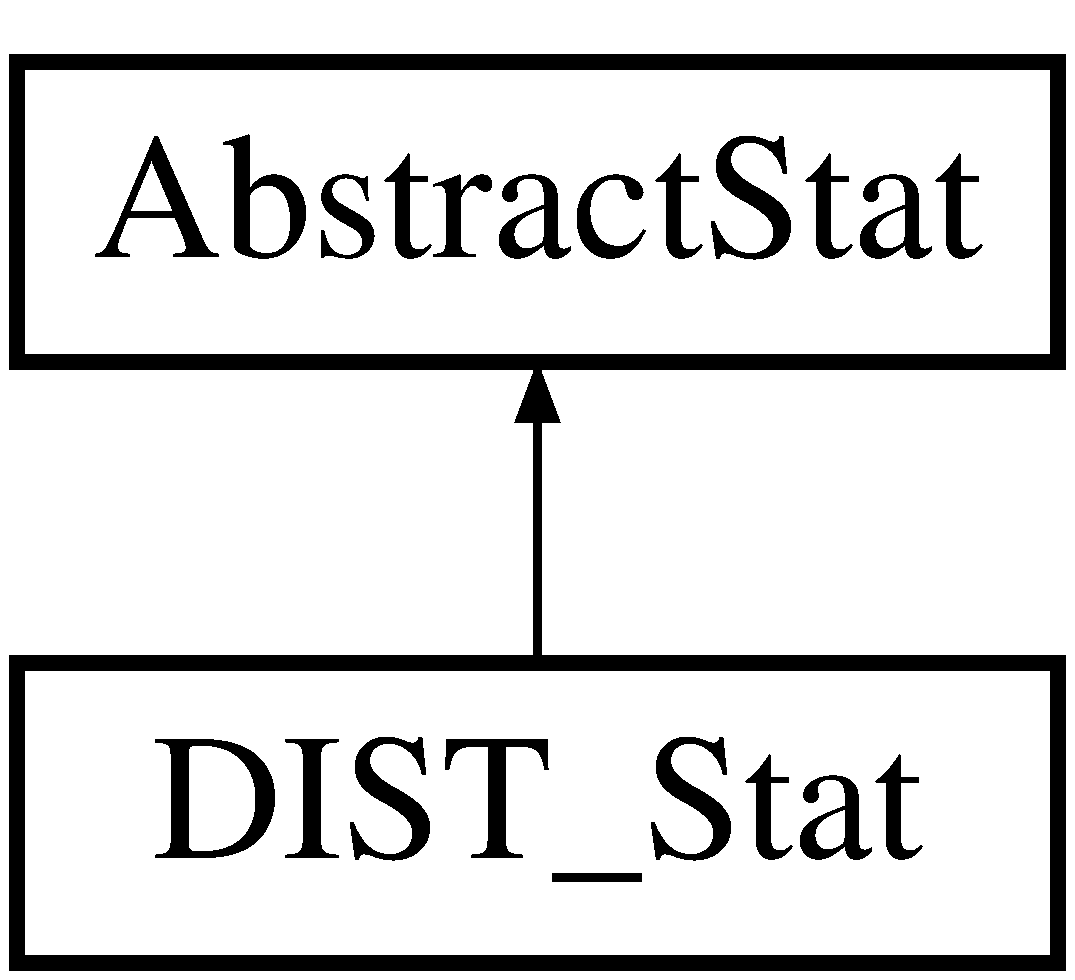
\includegraphics[height=2.000000cm]{classDIST__Stat}
\end{center}
\end{figure}
\subsection*{Public Member Functions}
\begin{DoxyCompactItemize}
\item 
\hyperlink{classDIST__Stat_a0ecccb2dc9ba814f9468d3f814329b04}{DIST\_\-Stat} (const string \&str, const string \&outputfilename, long ID, \hyperlink{classProcessorStatistics}{ProcessorStatistics} $\ast$procStat)
\item 
virtual \hyperlink{classDIST__Stat_a223d849dc2df71d9909a5833bf17beb9}{$\sim$DIST\_\-Stat} ()
\item 
virtual \hyperlink{classAbstractStat}{AbstractStat} $\ast$ \hyperlink{classDIST__Stat_a11f5f75a5f6d8551e342a23e72f27809}{clone} (unsigned int coreID)
\item 
void \hyperlink{classDIST__Stat_a04d60f3b378b7c9439039abe2e2019d0}{addMember} (long memberID)
\item 
virtual void \hyperlink{classDIST__Stat_a521cb2140eba939df71b12dfe805386a}{writeTo} (ofstream \&stream)
\end{DoxyCompactItemize}
\subsection*{Private Attributes}
\begin{DoxyCompactItemize}
\item 
vector$<$ long $>$ \hyperlink{classDIST__Stat_a66b040153f6d5636d372b5bb3f0c6802}{m\_\-distributionMembers}
\item 
\hyperlink{classProcessorStatistics}{ProcessorStatistics} $\ast$ \hyperlink{classDIST__Stat_a867cb02e1feb40c13b29ab79746853e6}{m\_\-ProcStat}
\end{DoxyCompactItemize}


\subsection{Detailed Description}
DIST type stat. 

\subsection{Constructor \& Destructor Documentation}
\hypertarget{classDIST__Stat_a0ecccb2dc9ba814f9468d3f814329b04}{
\index{DIST\_\-Stat@{DIST\_\-Stat}!DIST\_\-Stat@{DIST\_\-Stat}}
\index{DIST\_\-Stat@{DIST\_\-Stat}!DIST_Stat@{DIST\_\-Stat}}
\subsubsection[{DIST\_\-Stat}]{\setlength{\rightskip}{0pt plus 5cm}DIST\_\-Stat::DIST\_\-Stat (
\begin{DoxyParamCaption}
\item[{const string \&}]{ str, }
\item[{const string \&}]{ outputfilename, }
\item[{long}]{ ID, }
\item[{{\bf ProcessorStatistics} $\ast$}]{ procStat}
\end{DoxyParamCaption}
)\hspace{0.3cm}{\ttfamily  \mbox{[}inline\mbox{]}}}}
\label{classDIST__Stat_a0ecccb2dc9ba814f9468d3f814329b04}
Constructor. \hypertarget{classDIST__Stat_a223d849dc2df71d9909a5833bf17beb9}{
\index{DIST\_\-Stat@{DIST\_\-Stat}!$\sim$DIST\_\-Stat@{$\sim$DIST\_\-Stat}}
\index{$\sim$DIST\_\-Stat@{$\sim$DIST\_\-Stat}!DIST_Stat@{DIST\_\-Stat}}
\subsubsection[{$\sim$DIST\_\-Stat}]{\setlength{\rightskip}{0pt plus 5cm}virtual DIST\_\-Stat::$\sim$DIST\_\-Stat (
\begin{DoxyParamCaption}
{}
\end{DoxyParamCaption}
)\hspace{0.3cm}{\ttfamily  \mbox{[}inline, virtual\mbox{]}}}}
\label{classDIST__Stat_a223d849dc2df71d9909a5833bf17beb9}
Destructor. 

\subsection{Member Function Documentation}
\hypertarget{classDIST__Stat_a04d60f3b378b7c9439039abe2e2019d0}{
\index{DIST\_\-Stat@{DIST\_\-Stat}!addMember@{addMember}}
\index{addMember@{addMember}!DIST_Stat@{DIST\_\-Stat}}
\subsubsection[{addMember}]{\setlength{\rightskip}{0pt plus 5cm}void DIST\_\-Stat::addMember (
\begin{DoxyParamCaption}
\item[{long}]{ memberID}
\end{DoxyParamCaption}
)\hspace{0.3cm}{\ttfamily  \mbox{[}inline\mbox{]}}}}
\label{classDIST__Stat_a04d60f3b378b7c9439039abe2e2019d0}
Add a new stat. \hypertarget{classDIST__Stat_a11f5f75a5f6d8551e342a23e72f27809}{
\index{DIST\_\-Stat@{DIST\_\-Stat}!clone@{clone}}
\index{clone@{clone}!DIST_Stat@{DIST\_\-Stat}}
\subsubsection[{clone}]{\setlength{\rightskip}{0pt plus 5cm}virtual {\bf AbstractStat}$\ast$ DIST\_\-Stat::clone (
\begin{DoxyParamCaption}
\item[{unsigned int}]{ coreID}
\end{DoxyParamCaption}
)\hspace{0.3cm}{\ttfamily  \mbox{[}inline, virtual\mbox{]}}}}
\label{classDIST__Stat_a11f5f75a5f6d8551e342a23e72f27809}
Clone a stat. 

Implements \hyperlink{classAbstractStat_aed9a458491d92fb2cc3c458990d9fab1}{AbstractStat}.

\hypertarget{classDIST__Stat_a521cb2140eba939df71b12dfe805386a}{
\index{DIST\_\-Stat@{DIST\_\-Stat}!writeTo@{writeTo}}
\index{writeTo@{writeTo}!DIST_Stat@{DIST\_\-Stat}}
\subsubsection[{writeTo}]{\setlength{\rightskip}{0pt plus 5cm}void DIST\_\-Stat::writeTo (
\begin{DoxyParamCaption}
\item[{ofstream \&}]{ stream}
\end{DoxyParamCaption}
)\hspace{0.3cm}{\ttfamily  \mbox{[}virtual\mbox{]}}}}
\label{classDIST__Stat_a521cb2140eba939df71b12dfe805386a}
Dump out all stats to the file. 

Reimplemented from \hyperlink{classAbstractStat_aa4760247da47c70d7345de5d881f59cb}{AbstractStat}.



\subsection{Member Data Documentation}
\hypertarget{classDIST__Stat_a66b040153f6d5636d372b5bb3f0c6802}{
\index{DIST\_\-Stat@{DIST\_\-Stat}!m\_\-distributionMembers@{m\_\-distributionMembers}}
\index{m\_\-distributionMembers@{m\_\-distributionMembers}!DIST_Stat@{DIST\_\-Stat}}
\subsubsection[{m\_\-distributionMembers}]{\setlength{\rightskip}{0pt plus 5cm}vector$<$long$>$ {\bf DIST\_\-Stat::m\_\-distributionMembers}\hspace{0.3cm}{\ttfamily  \mbox{[}private\mbox{]}}}}
\label{classDIST__Stat_a66b040153f6d5636d372b5bb3f0c6802}
stat table \hypertarget{classDIST__Stat_a867cb02e1feb40c13b29ab79746853e6}{
\index{DIST\_\-Stat@{DIST\_\-Stat}!m\_\-ProcStat@{m\_\-ProcStat}}
\index{m\_\-ProcStat@{m\_\-ProcStat}!DIST_Stat@{DIST\_\-Stat}}
\subsubsection[{m\_\-ProcStat}]{\setlength{\rightskip}{0pt plus 5cm}{\bf ProcessorStatistics}$\ast$ {\bf DIST\_\-Stat::m\_\-ProcStat}\hspace{0.3cm}{\ttfamily  \mbox{[}private\mbox{]}}}}
\label{classDIST__Stat_a867cb02e1feb40c13b29ab79746853e6}
reference to simulation-\/scoped processor stats 

The documentation for this class was generated from the following files:\begin{DoxyCompactItemize}
\item 
statistics.h\item 
statistics.cc\end{DoxyCompactItemize}

\hypertarget{classDISTMember__Stat}{
\section{DISTMember\_\-Stat Class Reference}
\label{classDISTMember__Stat}\index{DISTMember\_\-Stat@{DISTMember\_\-Stat}}
}


Distribution member class.  




{\ttfamily \#include $<$statistics.h$>$}

Inheritance diagram for DISTMember\_\-Stat:\begin{figure}[H]
\begin{center}
\leavevmode
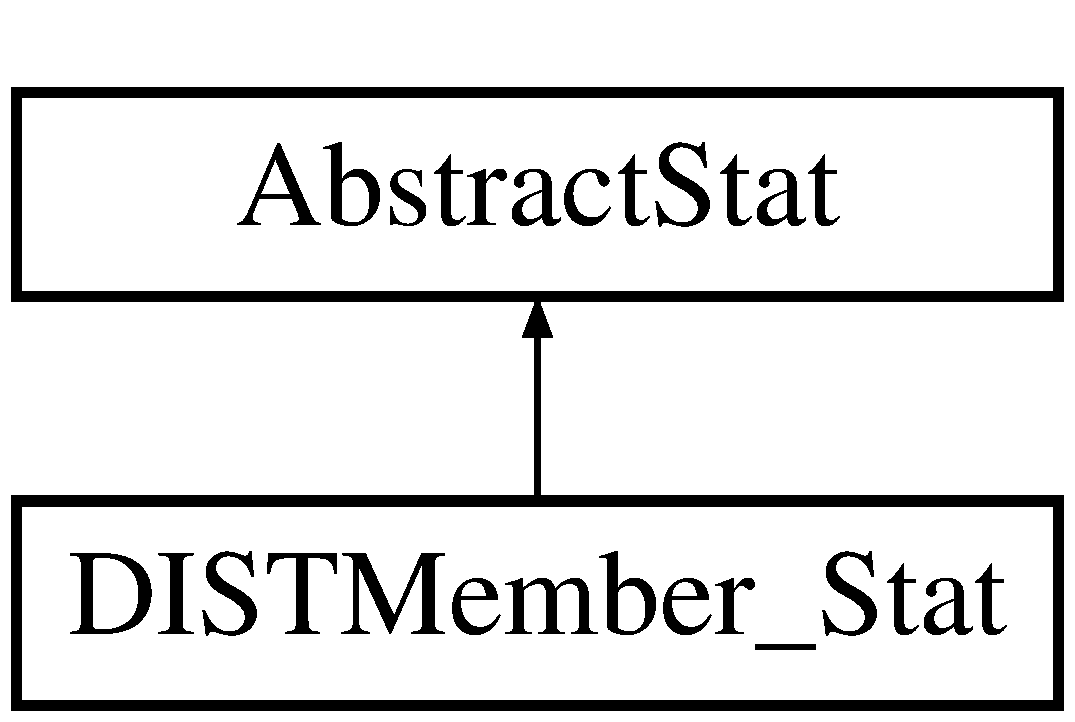
\includegraphics[height=2.000000cm]{classDISTMember__Stat}
\end{center}
\end{figure}
\subsection*{Public Member Functions}
\begin{DoxyCompactItemize}
\item 
\hyperlink{classDISTMember__Stat_a42b92bba8d7d564ead7e520a071fbb92}{DISTMember\_\-Stat} (const string \&str, const string \&outputfilename, long ID, long distID, bool coreWide=false, bool isTemplate=false)
\item 
virtual \hyperlink{classDISTMember__Stat_a499ff709db253422a0ba3d249fd9f828}{$\sim$DISTMember\_\-Stat} ()
\item 
virtual bool \hyperlink{classDISTMember__Stat_a0b0238ffd723c62d9f1d52c7499296c0}{memberOfDistribution} ()
\item 
void \hyperlink{classDISTMember__Stat_ad23f94e3c35b4009cd87490eded85bfc}{setParentDistroID} (long ID)
\item 
virtual \hyperlink{classAbstractStat}{AbstractStat} $\ast$ \hyperlink{classDISTMember__Stat_a3a20618868cfc2ac768e0e640049ffad}{clone} (unsigned int coreID)
\end{DoxyCompactItemize}
\subsection*{Private Attributes}
\begin{DoxyCompactItemize}
\item 
long \hyperlink{classDISTMember__Stat_a161cdc74a36982281bcbfb0240509f44}{m\_\-parentDistroID}
\end{DoxyCompactItemize}
\subsection*{Friends}
\begin{DoxyCompactItemize}
\item 
\hypertarget{classDISTMember__Stat_a27a5e86239948375f8e485e6247a0d85}{
class \hyperlink{classDISTMember__Stat_a27a5e86239948375f8e485e6247a0d85}{DIST\_\-Stat}}
\label{classDISTMember__Stat_a27a5e86239948375f8e485e6247a0d85}

\end{DoxyCompactItemize}


\subsection{Detailed Description}
Distribution member class. 

\subsection{Constructor \& Destructor Documentation}
\hypertarget{classDISTMember__Stat_a42b92bba8d7d564ead7e520a071fbb92}{
\index{DISTMember\_\-Stat@{DISTMember\_\-Stat}!DISTMember\_\-Stat@{DISTMember\_\-Stat}}
\index{DISTMember\_\-Stat@{DISTMember\_\-Stat}!DISTMember_Stat@{DISTMember\_\-Stat}}
\subsubsection[{DISTMember\_\-Stat}]{\setlength{\rightskip}{0pt plus 5cm}DISTMember\_\-Stat::DISTMember\_\-Stat (
\begin{DoxyParamCaption}
\item[{const string \&}]{ str, }
\item[{const string \&}]{ outputfilename, }
\item[{long}]{ ID, }
\item[{long}]{ distID, }
\item[{bool}]{ coreWide = {\ttfamily false}, }
\item[{bool}]{ isTemplate = {\ttfamily false}}
\end{DoxyParamCaption}
)\hspace{0.3cm}{\ttfamily  \mbox{[}inline\mbox{]}}}}
\label{classDISTMember__Stat_a42b92bba8d7d564ead7e520a071fbb92}
Constructor. \hypertarget{classDISTMember__Stat_a499ff709db253422a0ba3d249fd9f828}{
\index{DISTMember\_\-Stat@{DISTMember\_\-Stat}!$\sim$DISTMember\_\-Stat@{$\sim$DISTMember\_\-Stat}}
\index{$\sim$DISTMember\_\-Stat@{$\sim$DISTMember\_\-Stat}!DISTMember_Stat@{DISTMember\_\-Stat}}
\subsubsection[{$\sim$DISTMember\_\-Stat}]{\setlength{\rightskip}{0pt plus 5cm}virtual DISTMember\_\-Stat::$\sim$DISTMember\_\-Stat (
\begin{DoxyParamCaption}
{}
\end{DoxyParamCaption}
)\hspace{0.3cm}{\ttfamily  \mbox{[}inline, virtual\mbox{]}}}}
\label{classDISTMember__Stat_a499ff709db253422a0ba3d249fd9f828}
Destructor. 

\subsection{Member Function Documentation}
\hypertarget{classDISTMember__Stat_a3a20618868cfc2ac768e0e640049ffad}{
\index{DISTMember\_\-Stat@{DISTMember\_\-Stat}!clone@{clone}}
\index{clone@{clone}!DISTMember_Stat@{DISTMember\_\-Stat}}
\subsubsection[{clone}]{\setlength{\rightskip}{0pt plus 5cm}virtual {\bf AbstractStat}$\ast$ DISTMember\_\-Stat::clone (
\begin{DoxyParamCaption}
\item[{unsigned int}]{ coreID}
\end{DoxyParamCaption}
)\hspace{0.3cm}{\ttfamily  \mbox{[}inline, virtual\mbox{]}}}}
\label{classDISTMember__Stat_a3a20618868cfc2ac768e0e640049ffad}
Clone a stat. 

Implements \hyperlink{classAbstractStat_aed9a458491d92fb2cc3c458990d9fab1}{AbstractStat}.

\hypertarget{classDISTMember__Stat_a0b0238ffd723c62d9f1d52c7499296c0}{
\index{DISTMember\_\-Stat@{DISTMember\_\-Stat}!memberOfDistribution@{memberOfDistribution}}
\index{memberOfDistribution@{memberOfDistribution}!DISTMember_Stat@{DISTMember\_\-Stat}}
\subsubsection[{memberOfDistribution}]{\setlength{\rightskip}{0pt plus 5cm}virtual bool DISTMember\_\-Stat::memberOfDistribution (
\begin{DoxyParamCaption}
{}
\end{DoxyParamCaption}
)\hspace{0.3cm}{\ttfamily  \mbox{[}inline, virtual\mbox{]}}}}
\label{classDISTMember__Stat_a0b0238ffd723c62d9f1d52c7499296c0}
Test this is the member of dist stat 

Reimplemented from \hyperlink{classAbstractStat_a8b819d1de7dd14edb854545329484506}{AbstractStat}.

\hypertarget{classDISTMember__Stat_ad23f94e3c35b4009cd87490eded85bfc}{
\index{DISTMember\_\-Stat@{DISTMember\_\-Stat}!setParentDistroID@{setParentDistroID}}
\index{setParentDistroID@{setParentDistroID}!DISTMember_Stat@{DISTMember\_\-Stat}}
\subsubsection[{setParentDistroID}]{\setlength{\rightskip}{0pt plus 5cm}void DISTMember\_\-Stat::setParentDistroID (
\begin{DoxyParamCaption}
\item[{long}]{ ID}
\end{DoxyParamCaption}
)\hspace{0.3cm}{\ttfamily  \mbox{[}inline\mbox{]}}}}
\label{classDISTMember__Stat_ad23f94e3c35b4009cd87490eded85bfc}
set parent dist id 

\subsection{Member Data Documentation}
\hypertarget{classDISTMember__Stat_a161cdc74a36982281bcbfb0240509f44}{
\index{DISTMember\_\-Stat@{DISTMember\_\-Stat}!m\_\-parentDistroID@{m\_\-parentDistroID}}
\index{m\_\-parentDistroID@{m\_\-parentDistroID}!DISTMember_Stat@{DISTMember\_\-Stat}}
\subsubsection[{m\_\-parentDistroID}]{\setlength{\rightskip}{0pt plus 5cm}long {\bf DISTMember\_\-Stat::m\_\-parentDistroID}\hspace{0.3cm}{\ttfamily  \mbox{[}private\mbox{]}}}}
\label{classDISTMember__Stat_a161cdc74a36982281bcbfb0240509f44}
parent distribution stat id 

The documentation for this class was generated from the following file:\begin{DoxyCompactItemize}
\item 
statistics.h\end{DoxyCompactItemize}

\hypertarget{classdram__controller__c}{
\section{dram\_\-controller\_\-c Class Reference}
\label{classdram__controller__c}\index{dram\_\-controller\_\-c@{dram\_\-controller\_\-c}}
}


Base dram scheduling class (FCFS).  




{\ttfamily \#include $<$dram.h$>$}

Inheritance diagram for dram\_\-controller\_\-c:\begin{figure}[H]
\begin{center}
\leavevmode
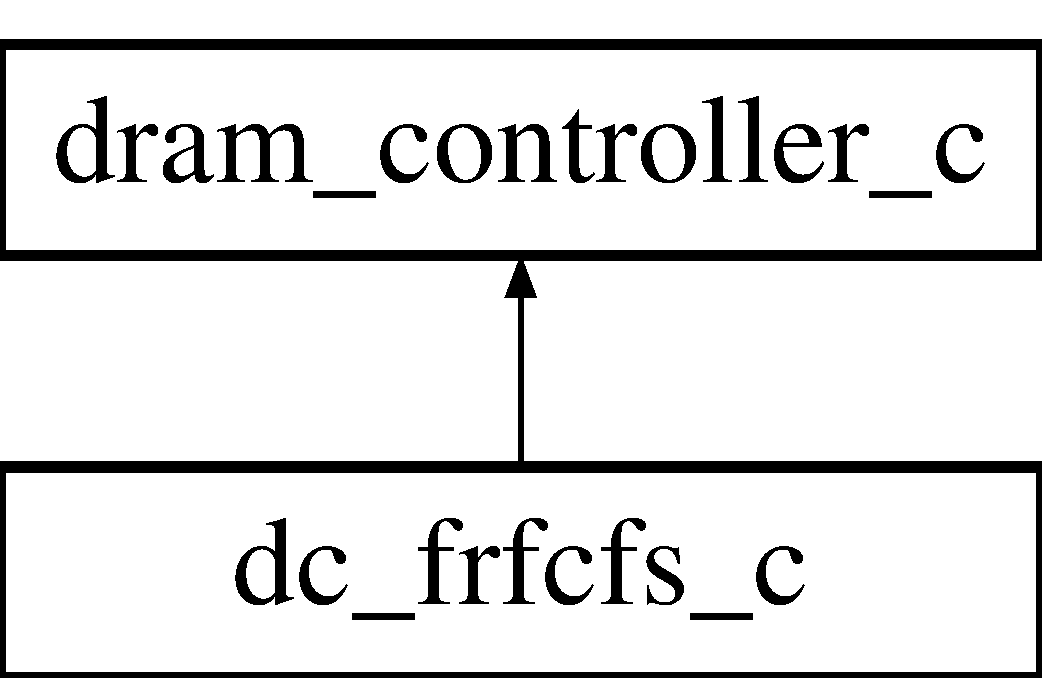
\includegraphics[height=2.000000cm]{classdram__controller__c}
\end{center}
\end{figure}
\subsection*{Public Member Functions}
\begin{DoxyCompactItemize}
\item 
\hyperlink{classdram__controller__c_a7248fd90d56110a6b7694546f9eb0d24}{dram\_\-controller\_\-c} (\hyperlink{classmacsim__c}{macsim\_\-c} $\ast$simBase)
\item 
virtual \hyperlink{classdram__controller__c_a1c1930981dac68e329b7fba36926fe4c}{$\sim$dram\_\-controller\_\-c} ()
\item 
void \hyperlink{classdram__controller__c_a6da28c92cae6664ba2850cb7940e8c26}{init} (int id, int noc\_\-id)
\item 
bool \hyperlink{classdram__controller__c_a49256d356f26730395d1f80ddbc4b9e6}{insert\_\-new\_\-req} (\hyperlink{structmem__req__s}{mem\_\-req\_\-s} $\ast$mem\_\-req)
\item 
void \hyperlink{classdram__controller__c_a7e9c891a53b54277e87564f4883adf4a}{insert\_\-req\_\-in\_\-drb} (\hyperlink{structmem__req__s}{mem\_\-req\_\-s} $\ast$req, int bid, int rid, int cid)
\item 
void \hyperlink{classdram__controller__c_a73581d9a96758d6f7fa8cc085a0cbddf}{run\_\-a\_\-cycle} ()
\item 
void \hyperlink{classdram__controller__c_aaff58a137e82a8096c8c66f58cdff99d}{create\_\-network\_\-interface} (void)
\item 
\hypertarget{classdram__controller__c_a26feec2184a215067af8e24839ab4044}{
void {\bfseries print\_\-req} (void)}
\label{classdram__controller__c_a26feec2184a215067af8e24839ab4044}

\end{DoxyCompactItemize}
\subsection*{Static Public Attributes}
\begin{DoxyCompactItemize}
\item 
static int {\bfseries dram\_\-req\_\-priority} \mbox{[}DRAM\_\-REQ\_\-PRIORITY\_\-COUNT\mbox{]}
\item 
static const char $\ast$ {\bfseries dram\_\-state} \mbox{[}DRAM\_\-STATE\_\-COUNT\mbox{]}
\end{DoxyCompactItemize}
\subsection*{Protected Member Functions}
\begin{DoxyCompactItemize}
\item 
void \hyperlink{classdram__controller__c_aa867d0ef9025402fd101fa6805b7eabc}{bank\_\-schedule} ()
\item 
void \hyperlink{classdram__controller__c_ac756549d7ec5f7fa43da299ed202a765}{bank\_\-schedule\_\-new} ()
\item 
void \hyperlink{classdram__controller__c_a841f14d3e9210fe4cf61c8f2af3c8a6e}{bank\_\-schedule\_\-complete} ()
\item 
virtual \hyperlink{structdrb__entry__s}{drb\_\-entry\_\-s} $\ast$ \hyperlink{classdram__controller__c_a0ce04de6742977e7c962ef977c1b9da0}{schedule} (list$<$ \hyperlink{structdrb__entry__s}{drb\_\-entry\_\-s} $\ast$ $>$ $\ast$drb\_\-list)
\item 
void \hyperlink{classdram__controller__c_a4bb5af511ad009ac4e74ce07e4df745f}{channel\_\-schedule} ()
\item 
void \hyperlink{classdram__controller__c_aed40936dd5ade7769eb84a8624dc06a8}{channel\_\-schedule\_\-cmd} ()
\item 
void \hyperlink{classdram__controller__c_aa33f2630c24db2bec43bccd6c8a5e3cc}{channel\_\-schedule\_\-data} ()
\item 
bool \hyperlink{classdram__controller__c_adee305e1751db04ee9db1ffd30caa6a5}{avail\_\-data\_\-bus} (int)
\item 
Counter \hyperlink{classdram__controller__c_a064fedf84d64d7addfeed1ac14c5b749}{acquire\_\-data\_\-bus} (int, int, bool gpu\_\-req)
\item 
void \hyperlink{classdram__controller__c_a97f17a711a47b54cc912c11192978d85}{flush\_\-prefetch} (int bid)
\item 
void \hyperlink{classdram__controller__c_a64503f53340c0f14ab7f5bc64d55777d}{progress\_\-check} ()
\item 
bool \hyperlink{classdram__controller__c_afc34a8f4247b6197ee16f33383366303}{send\_\-packet} (\hyperlink{structdrb__entry__s}{drb\_\-entry\_\-s} $\ast$req)
\item 
void \hyperlink{classdram__controller__c_af4ab757ab961800b38c1a5602419c59f}{receive\_\-packet} (void)
\item 
virtual void \hyperlink{classdram__controller__c_a817c599eb63d1545e3351003fdf6da76}{on\_\-insert} (\hyperlink{structmem__req__s}{mem\_\-req\_\-s} $\ast$req, int bid, int rid, int cid)
\item 
virtual void \hyperlink{classdram__controller__c_ab9a5c51da823023ca5f0a3dbb68a8856}{on\_\-complete} (\hyperlink{structdrb__entry__s}{drb\_\-entry\_\-s} $\ast$req)
\item 
virtual void \hyperlink{classdram__controller__c_a27a7f5cb6b2a8666f4444816c0c86ba1}{on\_\-run\_\-a\_\-cycle} ()
\end{DoxyCompactItemize}
\subsection*{Protected Attributes}
\begin{DoxyCompactItemize}
\item 
list$<$ \hyperlink{structdrb__entry__s}{drb\_\-entry\_\-s} $\ast$ $>$ $\ast$ \hyperlink{classdram__controller__c_ae827da2c640a345b548f55c4619df6c3}{m\_\-buffer}
\item 
list$<$ \hyperlink{structdrb__entry__s}{drb\_\-entry\_\-s} $\ast$ $>$ $\ast$ \hyperlink{classdram__controller__c_a62d96cc25786a499d89ae5d17732e532}{m\_\-buffer\_\-free\_\-list}
\item 
\hyperlink{structdrb__entry__s}{drb\_\-entry\_\-s} $\ast$$\ast$ \hyperlink{classdram__controller__c_a52b6d16df53c6b0482cbdc782719d3dc}{m\_\-current\_\-list}
\item 
int $\ast$ \hyperlink{classdram__controller__c_a7b69bd4b34ed9754a30e69e0bdebb609}{m\_\-current\_\-rid}
\item 
Counter $\ast$ \hyperlink{classdram__controller__c_ad4f31c52a4c3858ae5fae007bc954c09}{m\_\-bank\_\-ready}
\item 
Counter $\ast$ \hyperlink{classdram__controller__c_a923a18758cbecc2b240c619309f82cdd}{m\_\-data\_\-ready}
\item 
Counter $\ast$ \hyperlink{classdram__controller__c_a9ff45b23f89fb48e07a21253a28d5903}{m\_\-data\_\-avail}
\item 
Counter $\ast$ \hyperlink{classdram__controller__c_ab0c72ef77bc137b1ed16a060dd622c84}{m\_\-bank\_\-timestamp}
\item 
int \hyperlink{classdram__controller__c_a88d2351690ac79425da4af48c28a55bd}{m\_\-bus\_\-width}
\item 
int $\ast$ \hyperlink{classdram__controller__c_add7d44dbb73dedd43c51a97ee1d0c17d}{m\_\-byte\_\-avail}
\item 
Counter $\ast$ \hyperlink{classdram__controller__c_aeff0032fc196b65007b89d00499c2bd1}{m\_\-dbus\_\-ready}
\item 
int \hyperlink{classdram__controller__c_a98fd7fb6cf778ca6bba63a861b551bda}{m\_\-num\_\-bank}
\item 
int \hyperlink{classdram__controller__c_a9a20ac3f7fa0c171702fc265f0ccc9bc}{m\_\-num\_\-channel}
\item 
int \hyperlink{classdram__controller__c_ac3907c9a15aa3131c9aee34313a28e37}{m\_\-num\_\-bank\_\-per\_\-channel}
\item 
uns \hyperlink{classdram__controller__c_ae55d96ec26968a1343ac0de05bd6485d}{m\_\-cid\_\-mask}
\item 
uns \hyperlink{classdram__controller__c_a433a0c33c4b2075c99ac4f7d489ec66b}{m\_\-bid\_\-mask}
\item 
uns \hyperlink{classdram__controller__c_ab181fe193cffbadab11d1c2252f071d9}{m\_\-bid\_\-shift}
\item 
uns \hyperlink{classdram__controller__c_a47129cd3d0467da1d6e53c928226858e}{m\_\-rid\_\-shift}
\item 
uns \hyperlink{classdram__controller__c_aa31c9a4e62e699e26dab2bc03487f71e}{m\_\-bid\_\-xor\_\-shift}
\item 
float \hyperlink{classdram__controller__c_af929273981621d260089ba6187e73b38}{m\_\-dram\_\-one\_\-cycle\_\-cpu}
\item 
int \hyperlink{classdram__controller__c_abb28f2d1c7793e514a005a7bc15589d9}{m\_\-activate\_\-latency\_\-cpu}
\item 
int \hyperlink{classdram__controller__c_aef712e15ee703272a9381b82cd487bcb}{m\_\-precharge\_\-latency\_\-cpu}
\item 
int \hyperlink{classdram__controller__c_a5f58c9560276617cab02c610b01b2cb1}{m\_\-column\_\-latency\_\-cpu}
\item 
float \hyperlink{classdram__controller__c_a33c4f9781f46ee69715f6ab54b4eec46}{m\_\-dram\_\-one\_\-cycle\_\-gpu}
\item 
int \hyperlink{classdram__controller__c_a835ddca91edbc43e049d625eff2207f8}{m\_\-activate\_\-latency\_\-gpu}
\item 
int \hyperlink{classdram__controller__c_aa61d120e34408419e0962dafb2681402}{m\_\-precharge\_\-latency\_\-gpu}
\item 
int \hyperlink{classdram__controller__c_a6b725908a9e2d0f284780dfa345d6160}{m\_\-column\_\-latency\_\-gpu}
\item 
int \hyperlink{classdram__controller__c_a7b3d7fc2ce0d87fa1ff76b4a6ba607a1}{m\_\-id}
\item 
int \hyperlink{classdram__controller__c_a86f6215cf918c0a83ca2180b8dcea67c}{m\_\-noc\_\-id}
\item 
int \hyperlink{classdram__controller__c_aaf23b00bc5d6622200397b680a4a7e76}{m\_\-num\_\-completed\_\-in\_\-last\_\-cycle}
\item 
int \hyperlink{classdram__controller__c_a7fc3aa259f15cd2f9cc87753d458f166}{m\_\-starvation\_\-cycle}
\item 
int \hyperlink{classdram__controller__c_a5b6f52c05df415ba22de7b0eab87acb0}{m\_\-total\_\-req}
\item 
ManifoldProcessor $\ast$ \hyperlink{classdram__controller__c_a572404de89967a3b7294080ff7390110}{m\_\-terminal}
\item 
\hypertarget{classdram__controller__c_a12525bd69d3b3d22b90fcf221e2ff4fe}{
\hyperlink{classrouter__c}{router\_\-c} $\ast$ {\bfseries m\_\-router}}
\label{classdram__controller__c_a12525bd69d3b3d22b90fcf221e2ff4fe}

\item 
\hypertarget{classdram__controller__c_a2e14886cc34935d940b0a0c406ae6665}{
Counter {\bfseries m\_\-avg\_\-latency}}
\label{classdram__controller__c_a2e14886cc34935d940b0a0c406ae6665}

\item 
\hypertarget{classdram__controller__c_a1c8073fe1d1fe865dca1cff3f1eb4f6b}{
Counter {\bfseries m\_\-avg\_\-latency\_\-base}}
\label{classdram__controller__c_a1c8073fe1d1fe865dca1cff3f1eb4f6b}

\item 
\hypertarget{classdram__controller__c_a4e4902d43276cfd78e3d9388739e0ede}{
int {\bfseries m\_\-prev\_\-avg\_\-latency}}
\label{classdram__controller__c_a4e4902d43276cfd78e3d9388739e0ede}

\item 
\hypertarget{classdram__controller__c_a40213c48bdc493fbe4648b3da9642f72}{
int {\bfseries m\_\-prev\_\-stable\_\-avg\_\-latency}}
\label{classdram__controller__c_a40213c48bdc493fbe4648b3da9642f72}

\item 
\hypertarget{classdram__controller__c_ac0f959af69fb479c5627fd0174de1303}{
Counter {\bfseries m\_\-band}}
\label{classdram__controller__c_ac0f959af69fb479c5627fd0174de1303}

\item 
\hypertarget{classdram__controller__c_ab2742462a8063fe548c4e4210a95d842}{
Counter {\bfseries m\_\-band\_\-base}}
\label{classdram__controller__c_ab2742462a8063fe548c4e4210a95d842}

\item 
\hypertarget{classdram__controller__c_aac6cfe0db40ab180e3a9d51153c3bb9f}{
int {\bfseries m\_\-prev\_\-band}}
\label{classdram__controller__c_aac6cfe0db40ab180e3a9d51153c3bb9f}

\item 
\hypertarget{classdram__controller__c_a7cf5af76731c5975cd312b623e4bf4dd}{
int {\bfseries m\_\-prev\_\-stable\_\-band}}
\label{classdram__controller__c_a7cf5af76731c5975cd312b623e4bf4dd}

\item 
\hypertarget{classdram__controller__c_a5ddb04828e9b538431f4f9c806d123ba}{
int {\bfseries m\_\-avg\_\-band}}
\label{classdram__controller__c_a5ddb04828e9b538431f4f9c806d123ba}

\item 
\hypertarget{classdram__controller__c_a30b56e08d35ee79d538098c6e35cee23}{
int {\bfseries m\_\-stable\_\-counter}}
\label{classdram__controller__c_a30b56e08d35ee79d538098c6e35cee23}

\item 
\hypertarget{classdram__controller__c_a297088370cd5062c233fcab06c693022}{
int {\bfseries m\_\-dram\_\-state}}
\label{classdram__controller__c_a297088370cd5062c233fcab06c693022}

\item 
\hypertarget{classdram__controller__c_ac50ba6ff0ee2de611a2c2d2ca6210bbf}{
ofstream {\bfseries temp\_\-out}}
\label{classdram__controller__c_ac50ba6ff0ee2de611a2c2d2ca6210bbf}

\item 
\hyperlink{classmacsim__c}{macsim\_\-c} $\ast$ \hyperlink{classdram__controller__c_ae96442e89de273175e8d2ee453a2c688}{m\_\-simBase}
\end{DoxyCompactItemize}


\subsection{Detailed Description}
Base dram scheduling class (FCFS). 

\subsection{Constructor \& Destructor Documentation}
\hypertarget{classdram__controller__c_a7248fd90d56110a6b7694546f9eb0d24}{
\index{dram\_\-controller\_\-c@{dram\_\-controller\_\-c}!dram\_\-controller\_\-c@{dram\_\-controller\_\-c}}
\index{dram\_\-controller\_\-c@{dram\_\-controller\_\-c}!dram_controller_c@{dram\_\-controller\_\-c}}
\subsubsection[{dram\_\-controller\_\-c}]{\setlength{\rightskip}{0pt plus 5cm}dram\_\-controller\_\-c::dram\_\-controller\_\-c (
\begin{DoxyParamCaption}
\item[{{\bf macsim\_\-c} $\ast$}]{ simBase}
\end{DoxyParamCaption}
)}}
\label{classdram__controller__c_a7248fd90d56110a6b7694546f9eb0d24}
Constructor. 
\begin{DoxyParams}{Parameters}
\item[{\em simBase}]-\/ Pointer to base simulation class for perf/stat counters \end{DoxyParams}
\hypertarget{classdram__controller__c_a1c1930981dac68e329b7fba36926fe4c}{
\index{dram\_\-controller\_\-c@{dram\_\-controller\_\-c}!$\sim$dram\_\-controller\_\-c@{$\sim$dram\_\-controller\_\-c}}
\index{$\sim$dram\_\-controller\_\-c@{$\sim$dram\_\-controller\_\-c}!dram_controller_c@{dram\_\-controller\_\-c}}
\subsubsection[{$\sim$dram\_\-controller\_\-c}]{\setlength{\rightskip}{0pt plus 5cm}dram\_\-controller\_\-c::$\sim$dram\_\-controller\_\-c (
\begin{DoxyParamCaption}
{}
\end{DoxyParamCaption}
)\hspace{0.3cm}{\ttfamily  \mbox{[}virtual\mbox{]}}}}
\label{classdram__controller__c_a1c1930981dac68e329b7fba36926fe4c}
virtual destructor. 

\subsection{Member Function Documentation}
\hypertarget{classdram__controller__c_a064fedf84d64d7addfeed1ac14c5b749}{
\index{dram\_\-controller\_\-c@{dram\_\-controller\_\-c}!acquire\_\-data\_\-bus@{acquire\_\-data\_\-bus}}
\index{acquire\_\-data\_\-bus@{acquire\_\-data\_\-bus}!dram_controller_c@{dram\_\-controller\_\-c}}
\subsubsection[{acquire\_\-data\_\-bus}]{\setlength{\rightskip}{0pt plus 5cm}Counter dram\_\-controller\_\-c::acquire\_\-data\_\-bus (
\begin{DoxyParamCaption}
\item[{int}]{ channel\_\-id, }
\item[{int}]{ req\_\-size, }
\item[{bool}]{ gpu\_\-req}
\end{DoxyParamCaption}
)\hspace{0.3cm}{\ttfamily  \mbox{[}protected\mbox{]}}}}
\label{classdram__controller__c_a064fedf84d64d7addfeed1ac14c5b749}
Acquire data bus access \hypertarget{classdram__controller__c_adee305e1751db04ee9db1ffd30caa6a5}{
\index{dram\_\-controller\_\-c@{dram\_\-controller\_\-c}!avail\_\-data\_\-bus@{avail\_\-data\_\-bus}}
\index{avail\_\-data\_\-bus@{avail\_\-data\_\-bus}!dram_controller_c@{dram\_\-controller\_\-c}}
\subsubsection[{avail\_\-data\_\-bus}]{\setlength{\rightskip}{0pt plus 5cm}bool dram\_\-controller\_\-c::avail\_\-data\_\-bus (
\begin{DoxyParamCaption}
\item[{int}]{ channel\_\-id}
\end{DoxyParamCaption}
)\hspace{0.3cm}{\ttfamily  \mbox{[}protected\mbox{]}}}}
\label{classdram__controller__c_adee305e1751db04ee9db1ffd30caa6a5}
Check whether data bus of a channel is available \hypertarget{classdram__controller__c_aa867d0ef9025402fd101fa6805b7eabc}{
\index{dram\_\-controller\_\-c@{dram\_\-controller\_\-c}!bank\_\-schedule@{bank\_\-schedule}}
\index{bank\_\-schedule@{bank\_\-schedule}!dram_controller_c@{dram\_\-controller\_\-c}}
\subsubsection[{bank\_\-schedule}]{\setlength{\rightskip}{0pt plus 5cm}void dram\_\-controller\_\-c::bank\_\-schedule (
\begin{DoxyParamCaption}
{}
\end{DoxyParamCaption}
)\hspace{0.3cm}{\ttfamily  \mbox{[}protected\mbox{]}}}}
\label{classdram__controller__c_aa867d0ef9025402fd101fa6805b7eabc}
Schedule each bank. \hypertarget{classdram__controller__c_a841f14d3e9210fe4cf61c8f2af3c8a6e}{
\index{dram\_\-controller\_\-c@{dram\_\-controller\_\-c}!bank\_\-schedule\_\-complete@{bank\_\-schedule\_\-complete}}
\index{bank\_\-schedule\_\-complete@{bank\_\-schedule\_\-complete}!dram_controller_c@{dram\_\-controller\_\-c}}
\subsubsection[{bank\_\-schedule\_\-complete}]{\setlength{\rightskip}{0pt plus 5cm}void dram\_\-controller\_\-c::bank\_\-schedule\_\-complete (
\begin{DoxyParamCaption}
\item[{void}]{}
\end{DoxyParamCaption}
)\hspace{0.3cm}{\ttfamily  \mbox{[}protected\mbox{]}}}}
\label{classdram__controller__c_a841f14d3e9210fe4cf61c8f2af3c8a6e}
Check whether previous request has been completed. \hypertarget{classdram__controller__c_ac756549d7ec5f7fa43da299ed202a765}{
\index{dram\_\-controller\_\-c@{dram\_\-controller\_\-c}!bank\_\-schedule\_\-new@{bank\_\-schedule\_\-new}}
\index{bank\_\-schedule\_\-new@{bank\_\-schedule\_\-new}!dram_controller_c@{dram\_\-controller\_\-c}}
\subsubsection[{bank\_\-schedule\_\-new}]{\setlength{\rightskip}{0pt plus 5cm}void dram\_\-controller\_\-c::bank\_\-schedule\_\-new (
\begin{DoxyParamCaption}
\item[{void}]{}
\end{DoxyParamCaption}
)\hspace{0.3cm}{\ttfamily  \mbox{[}protected\mbox{]}}}}
\label{classdram__controller__c_ac756549d7ec5f7fa43da299ed202a765}
When the previous request has been serviced, pick a new one based on the policy. \hypertarget{classdram__controller__c_a4bb5af511ad009ac4e74ce07e4df745f}{
\index{dram\_\-controller\_\-c@{dram\_\-controller\_\-c}!channel\_\-schedule@{channel\_\-schedule}}
\index{channel\_\-schedule@{channel\_\-schedule}!dram_controller_c@{dram\_\-controller\_\-c}}
\subsubsection[{channel\_\-schedule}]{\setlength{\rightskip}{0pt plus 5cm}void dram\_\-controller\_\-c::channel\_\-schedule (
\begin{DoxyParamCaption}
\item[{void}]{}
\end{DoxyParamCaption}
)\hspace{0.3cm}{\ttfamily  \mbox{[}protected\mbox{]}}}}
\label{classdram__controller__c_a4bb5af511ad009ac4e74ce07e4df745f}
Schedule each dram channel \hypertarget{classdram__controller__c_aed40936dd5ade7769eb84a8624dc06a8}{
\index{dram\_\-controller\_\-c@{dram\_\-controller\_\-c}!channel\_\-schedule\_\-cmd@{channel\_\-schedule\_\-cmd}}
\index{channel\_\-schedule\_\-cmd@{channel\_\-schedule\_\-cmd}!dram_controller_c@{dram\_\-controller\_\-c}}
\subsubsection[{channel\_\-schedule\_\-cmd}]{\setlength{\rightskip}{0pt plus 5cm}void dram\_\-controller\_\-c::channel\_\-schedule\_\-cmd (
\begin{DoxyParamCaption}
\item[{void}]{}
\end{DoxyParamCaption}
)\hspace{0.3cm}{\ttfamily  \mbox{[}protected\mbox{]}}}}
\label{classdram__controller__c_aed40936dd5ade7769eb84a8624dc06a8}
Pick a command from banks \hypertarget{classdram__controller__c_aa33f2630c24db2bec43bccd6c8a5e3cc}{
\index{dram\_\-controller\_\-c@{dram\_\-controller\_\-c}!channel\_\-schedule\_\-data@{channel\_\-schedule\_\-data}}
\index{channel\_\-schedule\_\-data@{channel\_\-schedule\_\-data}!dram_controller_c@{dram\_\-controller\_\-c}}
\subsubsection[{channel\_\-schedule\_\-data}]{\setlength{\rightskip}{0pt plus 5cm}void dram\_\-controller\_\-c::channel\_\-schedule\_\-data (
\begin{DoxyParamCaption}
\item[{void}]{}
\end{DoxyParamCaption}
)\hspace{0.3cm}{\ttfamily  \mbox{[}protected\mbox{]}}}}
\label{classdram__controller__c_aa33f2630c24db2bec43bccd6c8a5e3cc}
Pick a data ready bank \hypertarget{classdram__controller__c_aaff58a137e82a8096c8c66f58cdff99d}{
\index{dram\_\-controller\_\-c@{dram\_\-controller\_\-c}!create\_\-network\_\-interface@{create\_\-network\_\-interface}}
\index{create\_\-network\_\-interface@{create\_\-network\_\-interface}!dram_controller_c@{dram\_\-controller\_\-c}}
\subsubsection[{create\_\-network\_\-interface}]{\setlength{\rightskip}{0pt plus 5cm}void dram\_\-controller\_\-c::create\_\-network\_\-interface (
\begin{DoxyParamCaption}
\item[{void}]{}
\end{DoxyParamCaption}
)}}
\label{classdram__controller__c_aaff58a137e82a8096c8c66f58cdff99d}
Create the network interface \hypertarget{classdram__controller__c_a97f17a711a47b54cc912c11192978d85}{
\index{dram\_\-controller\_\-c@{dram\_\-controller\_\-c}!flush\_\-prefetch@{flush\_\-prefetch}}
\index{flush\_\-prefetch@{flush\_\-prefetch}!dram_controller_c@{dram\_\-controller\_\-c}}
\subsubsection[{flush\_\-prefetch}]{\setlength{\rightskip}{0pt plus 5cm}void dram\_\-controller\_\-c::flush\_\-prefetch (
\begin{DoxyParamCaption}
\item[{int}]{ bid}
\end{DoxyParamCaption}
)\hspace{0.3cm}{\ttfamily  \mbox{[}protected\mbox{]}}}}
\label{classdram__controller__c_a97f17a711a47b54cc912c11192978d85}
When a buffer is full, flush all prefetches in the buffer \hypertarget{classdram__controller__c_a6da28c92cae6664ba2850cb7940e8c26}{
\index{dram\_\-controller\_\-c@{dram\_\-controller\_\-c}!init@{init}}
\index{init@{init}!dram_controller_c@{dram\_\-controller\_\-c}}
\subsubsection[{init}]{\setlength{\rightskip}{0pt plus 5cm}void dram\_\-controller\_\-c::init (
\begin{DoxyParamCaption}
\item[{int}]{ id, }
\item[{int}]{ noc\_\-id}
\end{DoxyParamCaption}
)}}
\label{classdram__controller__c_a6da28c92cae6664ba2850cb7940e8c26}
Initialize a dram controller with network id and controller id. \hypertarget{classdram__controller__c_a49256d356f26730395d1f80ddbc4b9e6}{
\index{dram\_\-controller\_\-c@{dram\_\-controller\_\-c}!insert\_\-new\_\-req@{insert\_\-new\_\-req}}
\index{insert\_\-new\_\-req@{insert\_\-new\_\-req}!dram_controller_c@{dram\_\-controller\_\-c}}
\subsubsection[{insert\_\-new\_\-req}]{\setlength{\rightskip}{0pt plus 5cm}bool dram\_\-controller\_\-c::insert\_\-new\_\-req (
\begin{DoxyParamCaption}
\item[{{\bf mem\_\-req\_\-s} $\ast$}]{ mem\_\-req}
\end{DoxyParamCaption}
)}}
\label{classdram__controller__c_a49256d356f26730395d1f80ddbc4b9e6}
Insert a new request from the memory system. \hypertarget{classdram__controller__c_a7e9c891a53b54277e87564f4883adf4a}{
\index{dram\_\-controller\_\-c@{dram\_\-controller\_\-c}!insert\_\-req\_\-in\_\-drb@{insert\_\-req\_\-in\_\-drb}}
\index{insert\_\-req\_\-in\_\-drb@{insert\_\-req\_\-in\_\-drb}!dram_controller_c@{dram\_\-controller\_\-c}}
\subsubsection[{insert\_\-req\_\-in\_\-drb}]{\setlength{\rightskip}{0pt plus 5cm}void dram\_\-controller\_\-c::insert\_\-req\_\-in\_\-drb (
\begin{DoxyParamCaption}
\item[{{\bf mem\_\-req\_\-s} $\ast$}]{ req, }
\item[{int}]{ bid, }
\item[{int}]{ rid, }
\item[{int}]{ cid}
\end{DoxyParamCaption}
)}}
\label{classdram__controller__c_a7e9c891a53b54277e87564f4883adf4a}
Insert a new request to dram request buffer (DRB). \hypertarget{classdram__controller__c_ab9a5c51da823023ca5f0a3dbb68a8856}{
\index{dram\_\-controller\_\-c@{dram\_\-controller\_\-c}!on\_\-complete@{on\_\-complete}}
\index{on\_\-complete@{on\_\-complete}!dram_controller_c@{dram\_\-controller\_\-c}}
\subsubsection[{on\_\-complete}]{\setlength{\rightskip}{0pt plus 5cm}void dram\_\-controller\_\-c::on\_\-complete (
\begin{DoxyParamCaption}
\item[{{\bf drb\_\-entry\_\-s} $\ast$}]{ req}
\end{DoxyParamCaption}
)\hspace{0.3cm}{\ttfamily  \mbox{[}protected, virtual\mbox{]}}}}
\label{classdram__controller__c_ab9a5c51da823023ca5f0a3dbb68a8856}
Function to do any book-\/keeping that might be needed by scheduling policies \hypertarget{classdram__controller__c_a817c599eb63d1545e3351003fdf6da76}{
\index{dram\_\-controller\_\-c@{dram\_\-controller\_\-c}!on\_\-insert@{on\_\-insert}}
\index{on\_\-insert@{on\_\-insert}!dram_controller_c@{dram\_\-controller\_\-c}}
\subsubsection[{on\_\-insert}]{\setlength{\rightskip}{0pt plus 5cm}void dram\_\-controller\_\-c::on\_\-insert (
\begin{DoxyParamCaption}
\item[{{\bf mem\_\-req\_\-s} $\ast$}]{ req, }
\item[{int}]{ bid, }
\item[{int}]{ rid, }
\item[{int}]{ cid}
\end{DoxyParamCaption}
)\hspace{0.3cm}{\ttfamily  \mbox{[}protected, virtual\mbox{]}}}}
\label{classdram__controller__c_a817c599eb63d1545e3351003fdf6da76}
Function to do any book-\/keeping that might be needed by scheduling policies \hypertarget{classdram__controller__c_a27a7f5cb6b2a8666f4444816c0c86ba1}{
\index{dram\_\-controller\_\-c@{dram\_\-controller\_\-c}!on\_\-run\_\-a\_\-cycle@{on\_\-run\_\-a\_\-cycle}}
\index{on\_\-run\_\-a\_\-cycle@{on\_\-run\_\-a\_\-cycle}!dram_controller_c@{dram\_\-controller\_\-c}}
\subsubsection[{on\_\-run\_\-a\_\-cycle}]{\setlength{\rightskip}{0pt plus 5cm}void dram\_\-controller\_\-c::on\_\-run\_\-a\_\-cycle (
\begin{DoxyParamCaption}
{}
\end{DoxyParamCaption}
)\hspace{0.3cm}{\ttfamily  \mbox{[}protected, virtual\mbox{]}}}}
\label{classdram__controller__c_a27a7f5cb6b2a8666f4444816c0c86ba1}
Function to do any book-\/keeping that might be needed by scheduling policies \hypertarget{classdram__controller__c_a64503f53340c0f14ab7f5bc64d55777d}{
\index{dram\_\-controller\_\-c@{dram\_\-controller\_\-c}!progress\_\-check@{progress\_\-check}}
\index{progress\_\-check@{progress\_\-check}!dram_controller_c@{dram\_\-controller\_\-c}}
\subsubsection[{progress\_\-check}]{\setlength{\rightskip}{0pt plus 5cm}void dram\_\-controller\_\-c::progress\_\-check (
\begin{DoxyParamCaption}
\item[{void}]{}
\end{DoxyParamCaption}
)\hspace{0.3cm}{\ttfamily  \mbox{[}protected\mbox{]}}}}
\label{classdram__controller__c_a64503f53340c0f14ab7f5bc64d55777d}
Check the progress of dram controller. Although there are requests, if no request has been serviced for certain cycles raise exception. \hypertarget{classdram__controller__c_af4ab757ab961800b38c1a5602419c59f}{
\index{dram\_\-controller\_\-c@{dram\_\-controller\_\-c}!receive\_\-packet@{receive\_\-packet}}
\index{receive\_\-packet@{receive\_\-packet}!dram_controller_c@{dram\_\-controller\_\-c}}
\subsubsection[{receive\_\-packet}]{\setlength{\rightskip}{0pt plus 5cm}void dram\_\-controller\_\-c::receive\_\-packet (
\begin{DoxyParamCaption}
\item[{void}]{}
\end{DoxyParamCaption}
)\hspace{0.3cm}{\ttfamily  \mbox{[}protected\mbox{]}}}}
\label{classdram__controller__c_af4ab757ab961800b38c1a5602419c59f}
Receive a packet from the NoC \hypertarget{classdram__controller__c_a73581d9a96758d6f7fa8cc085a0cbddf}{
\index{dram\_\-controller\_\-c@{dram\_\-controller\_\-c}!run\_\-a\_\-cycle@{run\_\-a\_\-cycle}}
\index{run\_\-a\_\-cycle@{run\_\-a\_\-cycle}!dram_controller_c@{dram\_\-controller\_\-c}}
\subsubsection[{run\_\-a\_\-cycle}]{\setlength{\rightskip}{0pt plus 5cm}void dram\_\-controller\_\-c::run\_\-a\_\-cycle (
\begin{DoxyParamCaption}
\item[{void}]{}
\end{DoxyParamCaption}
)}}
\label{classdram__controller__c_a73581d9a96758d6f7fa8cc085a0cbddf}
Tick a cycle. \hypertarget{classdram__controller__c_a0ce04de6742977e7c962ef977c1b9da0}{
\index{dram\_\-controller\_\-c@{dram\_\-controller\_\-c}!schedule@{schedule}}
\index{schedule@{schedule}!dram_controller_c@{dram\_\-controller\_\-c}}
\subsubsection[{schedule}]{\setlength{\rightskip}{0pt plus 5cm}{\bf drb\_\-entry\_\-s} $\ast$ dram\_\-controller\_\-c::schedule (
\begin{DoxyParamCaption}
\item[{list$<$ {\bf drb\_\-entry\_\-s} $\ast$ $>$ $\ast$}]{ drb\_\-list}
\end{DoxyParamCaption}
)\hspace{0.3cm}{\ttfamily  \mbox{[}protected, virtual\mbox{]}}}}
\label{classdram__controller__c_a0ce04de6742977e7c962ef977c1b9da0}
Pick the highest priority entry based one the policy. Each dram scheduling policy should override this function. 

Reimplemented in \hyperlink{classdc__frfcfs__c_a4ee4def84ca42d169c13aec01590eeb8}{dc\_\-frfcfs\_\-c}.

\hypertarget{classdram__controller__c_afc34a8f4247b6197ee16f33383366303}{
\index{dram\_\-controller\_\-c@{dram\_\-controller\_\-c}!send\_\-packet@{send\_\-packet}}
\index{send\_\-packet@{send\_\-packet}!dram_controller_c@{dram\_\-controller\_\-c}}
\subsubsection[{send\_\-packet}]{\setlength{\rightskip}{0pt plus 5cm}bool dram\_\-controller\_\-c::send\_\-packet (
\begin{DoxyParamCaption}
\item[{{\bf drb\_\-entry\_\-s} $\ast$}]{ req}
\end{DoxyParamCaption}
)\hspace{0.3cm}{\ttfamily  \mbox{[}protected\mbox{]}}}}
\label{classdram__controller__c_afc34a8f4247b6197ee16f33383366303}
Send a packet to the NoC 
\begin{DoxyParams}{Parameters}
\item[{\em req}]memory request \end{DoxyParams}


\subsection{Member Data Documentation}
\hypertarget{classdram__controller__c_aceae2c83e6d35b3408b2b04efc8530b0}{
\index{dram\_\-controller\_\-c@{dram\_\-controller\_\-c}!dram\_\-req\_\-priority@{dram\_\-req\_\-priority}}
\index{dram\_\-req\_\-priority@{dram\_\-req\_\-priority}!dram_controller_c@{dram\_\-controller\_\-c}}
\subsubsection[{dram\_\-req\_\-priority}]{\setlength{\rightskip}{0pt plus 5cm}int dram\_\-controller\_\-c::dram\_\-req\_\-priority\hspace{0.3cm}{\ttfamily  \mbox{[}static\mbox{]}}}}
\label{classdram__controller__c_aceae2c83e6d35b3408b2b04efc8530b0}
{\bfseries Initial value:}
\begin{DoxyCode}
 
{
  0, 
  0, 
  0, 
  0, 
  0, 
  0, 
  0, 
  0, 
  0, 
  0, 
  0, 
  0  
}
\end{DoxyCode}
\hypertarget{classdram__controller__c_a5446c9ac632452dd729e7fed183fc443}{
\index{dram\_\-controller\_\-c@{dram\_\-controller\_\-c}!dram\_\-state@{dram\_\-state}}
\index{dram\_\-state@{dram\_\-state}!dram_controller_c@{dram\_\-controller\_\-c}}
\subsubsection[{dram\_\-state}]{\setlength{\rightskip}{0pt plus 5cm}const char $\ast$ dram\_\-controller\_\-c::dram\_\-state\hspace{0.3cm}{\ttfamily  \mbox{[}static\mbox{]}}}}
\label{classdram__controller__c_a5446c9ac632452dd729e7fed183fc443}
{\bfseries Initial value:}
\begin{DoxyCode}
 {
  "DRAM_INIT",
  "DRAM_CMD",
  "DRAM_CMD_WAIT",
  "DRAM_DATA",
  "DRAM_DATA_WAIT"
}
\end{DoxyCode}
\hypertarget{classdram__controller__c_abb28f2d1c7793e514a005a7bc15589d9}{
\index{dram\_\-controller\_\-c@{dram\_\-controller\_\-c}!m\_\-activate\_\-latency\_\-cpu@{m\_\-activate\_\-latency\_\-cpu}}
\index{m\_\-activate\_\-latency\_\-cpu@{m\_\-activate\_\-latency\_\-cpu}!dram_controller_c@{dram\_\-controller\_\-c}}
\subsubsection[{m\_\-activate\_\-latency\_\-cpu}]{\setlength{\rightskip}{0pt plus 5cm}int {\bf dram\_\-controller\_\-c::m\_\-activate\_\-latency\_\-cpu}\hspace{0.3cm}{\ttfamily  \mbox{[}protected\mbox{]}}}}
\label{classdram__controller__c_abb28f2d1c7793e514a005a7bc15589d9}
ACT latency \hypertarget{classdram__controller__c_a835ddca91edbc43e049d625eff2207f8}{
\index{dram\_\-controller\_\-c@{dram\_\-controller\_\-c}!m\_\-activate\_\-latency\_\-gpu@{m\_\-activate\_\-latency\_\-gpu}}
\index{m\_\-activate\_\-latency\_\-gpu@{m\_\-activate\_\-latency\_\-gpu}!dram_controller_c@{dram\_\-controller\_\-c}}
\subsubsection[{m\_\-activate\_\-latency\_\-gpu}]{\setlength{\rightskip}{0pt plus 5cm}int {\bf dram\_\-controller\_\-c::m\_\-activate\_\-latency\_\-gpu}\hspace{0.3cm}{\ttfamily  \mbox{[}protected\mbox{]}}}}
\label{classdram__controller__c_a835ddca91edbc43e049d625eff2207f8}
ACT latency \hypertarget{classdram__controller__c_ad4f31c52a4c3858ae5fae007bc954c09}{
\index{dram\_\-controller\_\-c@{dram\_\-controller\_\-c}!m\_\-bank\_\-ready@{m\_\-bank\_\-ready}}
\index{m\_\-bank\_\-ready@{m\_\-bank\_\-ready}!dram_controller_c@{dram\_\-controller\_\-c}}
\subsubsection[{m\_\-bank\_\-ready}]{\setlength{\rightskip}{0pt plus 5cm}Counter$\ast$ {\bf dram\_\-controller\_\-c::m\_\-bank\_\-ready}\hspace{0.3cm}{\ttfamily  \mbox{[}protected\mbox{]}}}}
\label{classdram__controller__c_ad4f31c52a4c3858ae5fae007bc954c09}
bank ready cycle \hypertarget{classdram__controller__c_ab0c72ef77bc137b1ed16a060dd622c84}{
\index{dram\_\-controller\_\-c@{dram\_\-controller\_\-c}!m\_\-bank\_\-timestamp@{m\_\-bank\_\-timestamp}}
\index{m\_\-bank\_\-timestamp@{m\_\-bank\_\-timestamp}!dram_controller_c@{dram\_\-controller\_\-c}}
\subsubsection[{m\_\-bank\_\-timestamp}]{\setlength{\rightskip}{0pt plus 5cm}Counter$\ast$ {\bf dram\_\-controller\_\-c::m\_\-bank\_\-timestamp}\hspace{0.3cm}{\ttfamily  \mbox{[}protected\mbox{]}}}}
\label{classdram__controller__c_ab0c72ef77bc137b1ed16a060dd622c84}
last touched cycle of a bank \hypertarget{classdram__controller__c_a433a0c33c4b2075c99ac4f7d489ec66b}{
\index{dram\_\-controller\_\-c@{dram\_\-controller\_\-c}!m\_\-bid\_\-mask@{m\_\-bid\_\-mask}}
\index{m\_\-bid\_\-mask@{m\_\-bid\_\-mask}!dram_controller_c@{dram\_\-controller\_\-c}}
\subsubsection[{m\_\-bid\_\-mask}]{\setlength{\rightskip}{0pt plus 5cm}uns {\bf dram\_\-controller\_\-c::m\_\-bid\_\-mask}\hspace{0.3cm}{\ttfamily  \mbox{[}protected\mbox{]}}}}
\label{classdram__controller__c_a433a0c33c4b2075c99ac4f7d489ec66b}
bank id mask \hypertarget{classdram__controller__c_ab181fe193cffbadab11d1c2252f071d9}{
\index{dram\_\-controller\_\-c@{dram\_\-controller\_\-c}!m\_\-bid\_\-shift@{m\_\-bid\_\-shift}}
\index{m\_\-bid\_\-shift@{m\_\-bid\_\-shift}!dram_controller_c@{dram\_\-controller\_\-c}}
\subsubsection[{m\_\-bid\_\-shift}]{\setlength{\rightskip}{0pt plus 5cm}uns {\bf dram\_\-controller\_\-c::m\_\-bid\_\-shift}\hspace{0.3cm}{\ttfamily  \mbox{[}protected\mbox{]}}}}
\label{classdram__controller__c_ab181fe193cffbadab11d1c2252f071d9}
bank id shift \hypertarget{classdram__controller__c_aa31c9a4e62e699e26dab2bc03487f71e}{
\index{dram\_\-controller\_\-c@{dram\_\-controller\_\-c}!m\_\-bid\_\-xor\_\-shift@{m\_\-bid\_\-xor\_\-shift}}
\index{m\_\-bid\_\-xor\_\-shift@{m\_\-bid\_\-xor\_\-shift}!dram_controller_c@{dram\_\-controller\_\-c}}
\subsubsection[{m\_\-bid\_\-xor\_\-shift}]{\setlength{\rightskip}{0pt plus 5cm}uns {\bf dram\_\-controller\_\-c::m\_\-bid\_\-xor\_\-shift}\hspace{0.3cm}{\ttfamily  \mbox{[}protected\mbox{]}}}}
\label{classdram__controller__c_aa31c9a4e62e699e26dab2bc03487f71e}
bank id xor factor \hypertarget{classdram__controller__c_ae827da2c640a345b548f55c4619df6c3}{
\index{dram\_\-controller\_\-c@{dram\_\-controller\_\-c}!m\_\-buffer@{m\_\-buffer}}
\index{m\_\-buffer@{m\_\-buffer}!dram_controller_c@{dram\_\-controller\_\-c}}
\subsubsection[{m\_\-buffer}]{\setlength{\rightskip}{0pt plus 5cm}list$<${\bf drb\_\-entry\_\-s}$\ast$$>$$\ast$ {\bf dram\_\-controller\_\-c::m\_\-buffer}\hspace{0.3cm}{\ttfamily  \mbox{[}protected\mbox{]}}}}
\label{classdram__controller__c_ae827da2c640a345b548f55c4619df6c3}
Dram request buffer (DRB) \hypertarget{classdram__controller__c_a62d96cc25786a499d89ae5d17732e532}{
\index{dram\_\-controller\_\-c@{dram\_\-controller\_\-c}!m\_\-buffer\_\-free\_\-list@{m\_\-buffer\_\-free\_\-list}}
\index{m\_\-buffer\_\-free\_\-list@{m\_\-buffer\_\-free\_\-list}!dram_controller_c@{dram\_\-controller\_\-c}}
\subsubsection[{m\_\-buffer\_\-free\_\-list}]{\setlength{\rightskip}{0pt plus 5cm}list$<${\bf drb\_\-entry\_\-s}$\ast$$>$$\ast$ {\bf dram\_\-controller\_\-c::m\_\-buffer\_\-free\_\-list}\hspace{0.3cm}{\ttfamily  \mbox{[}protected\mbox{]}}}}
\label{classdram__controller__c_a62d96cc25786a499d89ae5d17732e532}
DRB free list \hypertarget{classdram__controller__c_a88d2351690ac79425da4af48c28a55bd}{
\index{dram\_\-controller\_\-c@{dram\_\-controller\_\-c}!m\_\-bus\_\-width@{m\_\-bus\_\-width}}
\index{m\_\-bus\_\-width@{m\_\-bus\_\-width}!dram_controller_c@{dram\_\-controller\_\-c}}
\subsubsection[{m\_\-bus\_\-width}]{\setlength{\rightskip}{0pt plus 5cm}int {\bf dram\_\-controller\_\-c::m\_\-bus\_\-width}\hspace{0.3cm}{\ttfamily  \mbox{[}protected\mbox{]}}}}
\label{classdram__controller__c_a88d2351690ac79425da4af48c28a55bd}
dram data bus width \hypertarget{classdram__controller__c_add7d44dbb73dedd43c51a97ee1d0c17d}{
\index{dram\_\-controller\_\-c@{dram\_\-controller\_\-c}!m\_\-byte\_\-avail@{m\_\-byte\_\-avail}}
\index{m\_\-byte\_\-avail@{m\_\-byte\_\-avail}!dram_controller_c@{dram\_\-controller\_\-c}}
\subsubsection[{m\_\-byte\_\-avail}]{\setlength{\rightskip}{0pt plus 5cm}int$\ast$ {\bf dram\_\-controller\_\-c::m\_\-byte\_\-avail}\hspace{0.3cm}{\ttfamily  \mbox{[}protected\mbox{]}}}}
\label{classdram__controller__c_add7d44dbb73dedd43c51a97ee1d0c17d}
number of available bytes of data bus \hypertarget{classdram__controller__c_ae55d96ec26968a1343ac0de05bd6485d}{
\index{dram\_\-controller\_\-c@{dram\_\-controller\_\-c}!m\_\-cid\_\-mask@{m\_\-cid\_\-mask}}
\index{m\_\-cid\_\-mask@{m\_\-cid\_\-mask}!dram_controller_c@{dram\_\-controller\_\-c}}
\subsubsection[{m\_\-cid\_\-mask}]{\setlength{\rightskip}{0pt plus 5cm}uns {\bf dram\_\-controller\_\-c::m\_\-cid\_\-mask}\hspace{0.3cm}{\ttfamily  \mbox{[}protected\mbox{]}}}}
\label{classdram__controller__c_ae55d96ec26968a1343ac0de05bd6485d}
column id mask \hypertarget{classdram__controller__c_a5f58c9560276617cab02c610b01b2cb1}{
\index{dram\_\-controller\_\-c@{dram\_\-controller\_\-c}!m\_\-column\_\-latency\_\-cpu@{m\_\-column\_\-latency\_\-cpu}}
\index{m\_\-column\_\-latency\_\-cpu@{m\_\-column\_\-latency\_\-cpu}!dram_controller_c@{dram\_\-controller\_\-c}}
\subsubsection[{m\_\-column\_\-latency\_\-cpu}]{\setlength{\rightskip}{0pt plus 5cm}int {\bf dram\_\-controller\_\-c::m\_\-column\_\-latency\_\-cpu}\hspace{0.3cm}{\ttfamily  \mbox{[}protected\mbox{]}}}}
\label{classdram__controller__c_a5f58c9560276617cab02c610b01b2cb1}
CAS latency \hypertarget{classdram__controller__c_a6b725908a9e2d0f284780dfa345d6160}{
\index{dram\_\-controller\_\-c@{dram\_\-controller\_\-c}!m\_\-column\_\-latency\_\-gpu@{m\_\-column\_\-latency\_\-gpu}}
\index{m\_\-column\_\-latency\_\-gpu@{m\_\-column\_\-latency\_\-gpu}!dram_controller_c@{dram\_\-controller\_\-c}}
\subsubsection[{m\_\-column\_\-latency\_\-gpu}]{\setlength{\rightskip}{0pt plus 5cm}int {\bf dram\_\-controller\_\-c::m\_\-column\_\-latency\_\-gpu}\hspace{0.3cm}{\ttfamily  \mbox{[}protected\mbox{]}}}}
\label{classdram__controller__c_a6b725908a9e2d0f284780dfa345d6160}
CAS latency \hypertarget{classdram__controller__c_a52b6d16df53c6b0482cbdc782719d3dc}{
\index{dram\_\-controller\_\-c@{dram\_\-controller\_\-c}!m\_\-current\_\-list@{m\_\-current\_\-list}}
\index{m\_\-current\_\-list@{m\_\-current\_\-list}!dram_controller_c@{dram\_\-controller\_\-c}}
\subsubsection[{m\_\-current\_\-list}]{\setlength{\rightskip}{0pt plus 5cm}{\bf drb\_\-entry\_\-s}$\ast$$\ast$ {\bf dram\_\-controller\_\-c::m\_\-current\_\-list}\hspace{0.3cm}{\ttfamily  \mbox{[}protected\mbox{]}}}}
\label{classdram__controller__c_a52b6d16df53c6b0482cbdc782719d3dc}
Currently servicing request in each DRB \hypertarget{classdram__controller__c_a7b69bd4b34ed9754a30e69e0bdebb609}{
\index{dram\_\-controller\_\-c@{dram\_\-controller\_\-c}!m\_\-current\_\-rid@{m\_\-current\_\-rid}}
\index{m\_\-current\_\-rid@{m\_\-current\_\-rid}!dram_controller_c@{dram\_\-controller\_\-c}}
\subsubsection[{m\_\-current\_\-rid}]{\setlength{\rightskip}{0pt plus 5cm}int$\ast$ {\bf dram\_\-controller\_\-c::m\_\-current\_\-rid}\hspace{0.3cm}{\ttfamily  \mbox{[}protected\mbox{]}}}}
\label{classdram__controller__c_a7b69bd4b34ed9754a30e69e0bdebb609}
Current open row id \hypertarget{classdram__controller__c_a9ff45b23f89fb48e07a21253a28d5903}{
\index{dram\_\-controller\_\-c@{dram\_\-controller\_\-c}!m\_\-data\_\-avail@{m\_\-data\_\-avail}}
\index{m\_\-data\_\-avail@{m\_\-data\_\-avail}!dram_controller_c@{dram\_\-controller\_\-c}}
\subsubsection[{m\_\-data\_\-avail}]{\setlength{\rightskip}{0pt plus 5cm}Counter$\ast$ {\bf dram\_\-controller\_\-c::m\_\-data\_\-avail}\hspace{0.3cm}{\ttfamily  \mbox{[}protected\mbox{]}}}}
\label{classdram__controller__c_a9ff45b23f89fb48e07a21253a28d5903}
data avail cycle \hypertarget{classdram__controller__c_a923a18758cbecc2b240c619309f82cdd}{
\index{dram\_\-controller\_\-c@{dram\_\-controller\_\-c}!m\_\-data\_\-ready@{m\_\-data\_\-ready}}
\index{m\_\-data\_\-ready@{m\_\-data\_\-ready}!dram_controller_c@{dram\_\-controller\_\-c}}
\subsubsection[{m\_\-data\_\-ready}]{\setlength{\rightskip}{0pt plus 5cm}Counter$\ast$ {\bf dram\_\-controller\_\-c::m\_\-data\_\-ready}\hspace{0.3cm}{\ttfamily  \mbox{[}protected\mbox{]}}}}
\label{classdram__controller__c_a923a18758cbecc2b240c619309f82cdd}
data ready cycle \hypertarget{classdram__controller__c_aeff0032fc196b65007b89d00499c2bd1}{
\index{dram\_\-controller\_\-c@{dram\_\-controller\_\-c}!m\_\-dbus\_\-ready@{m\_\-dbus\_\-ready}}
\index{m\_\-dbus\_\-ready@{m\_\-dbus\_\-ready}!dram_controller_c@{dram\_\-controller\_\-c}}
\subsubsection[{m\_\-dbus\_\-ready}]{\setlength{\rightskip}{0pt plus 5cm}Counter$\ast$ {\bf dram\_\-controller\_\-c::m\_\-dbus\_\-ready}\hspace{0.3cm}{\ttfamily  \mbox{[}protected\mbox{]}}}}
\label{classdram__controller__c_aeff0032fc196b65007b89d00499c2bd1}
bus ready cycle \hypertarget{classdram__controller__c_af929273981621d260089ba6187e73b38}{
\index{dram\_\-controller\_\-c@{dram\_\-controller\_\-c}!m\_\-dram\_\-one\_\-cycle\_\-cpu@{m\_\-dram\_\-one\_\-cycle\_\-cpu}}
\index{m\_\-dram\_\-one\_\-cycle\_\-cpu@{m\_\-dram\_\-one\_\-cycle\_\-cpu}!dram_controller_c@{dram\_\-controller\_\-c}}
\subsubsection[{m\_\-dram\_\-one\_\-cycle\_\-cpu}]{\setlength{\rightskip}{0pt plus 5cm}float {\bf dram\_\-controller\_\-c::m\_\-dram\_\-one\_\-cycle\_\-cpu}\hspace{0.3cm}{\ttfamily  \mbox{[}protected\mbox{]}}}}
\label{classdram__controller__c_af929273981621d260089ba6187e73b38}
relative dram cycle to cpu cycle \hypertarget{classdram__controller__c_a33c4f9781f46ee69715f6ab54b4eec46}{
\index{dram\_\-controller\_\-c@{dram\_\-controller\_\-c}!m\_\-dram\_\-one\_\-cycle\_\-gpu@{m\_\-dram\_\-one\_\-cycle\_\-gpu}}
\index{m\_\-dram\_\-one\_\-cycle\_\-gpu@{m\_\-dram\_\-one\_\-cycle\_\-gpu}!dram_controller_c@{dram\_\-controller\_\-c}}
\subsubsection[{m\_\-dram\_\-one\_\-cycle\_\-gpu}]{\setlength{\rightskip}{0pt plus 5cm}float {\bf dram\_\-controller\_\-c::m\_\-dram\_\-one\_\-cycle\_\-gpu}\hspace{0.3cm}{\ttfamily  \mbox{[}protected\mbox{]}}}}
\label{classdram__controller__c_a33c4f9781f46ee69715f6ab54b4eec46}
relative dram cycle to cpu cycle \hypertarget{classdram__controller__c_a7b3d7fc2ce0d87fa1ff76b4a6ba607a1}{
\index{dram\_\-controller\_\-c@{dram\_\-controller\_\-c}!m\_\-id@{m\_\-id}}
\index{m\_\-id@{m\_\-id}!dram_controller_c@{dram\_\-controller\_\-c}}
\subsubsection[{m\_\-id}]{\setlength{\rightskip}{0pt plus 5cm}int {\bf dram\_\-controller\_\-c::m\_\-id}\hspace{0.3cm}{\ttfamily  \mbox{[}protected\mbox{]}}}}
\label{classdram__controller__c_a7b3d7fc2ce0d87fa1ff76b4a6ba607a1}
dram controller id \hypertarget{classdram__controller__c_a86f6215cf918c0a83ca2180b8dcea67c}{
\index{dram\_\-controller\_\-c@{dram\_\-controller\_\-c}!m\_\-noc\_\-id@{m\_\-noc\_\-id}}
\index{m\_\-noc\_\-id@{m\_\-noc\_\-id}!dram_controller_c@{dram\_\-controller\_\-c}}
\subsubsection[{m\_\-noc\_\-id}]{\setlength{\rightskip}{0pt plus 5cm}int {\bf dram\_\-controller\_\-c::m\_\-noc\_\-id}\hspace{0.3cm}{\ttfamily  \mbox{[}protected\mbox{]}}}}
\label{classdram__controller__c_a86f6215cf918c0a83ca2180b8dcea67c}
network id \hypertarget{classdram__controller__c_a98fd7fb6cf778ca6bba63a861b551bda}{
\index{dram\_\-controller\_\-c@{dram\_\-controller\_\-c}!m\_\-num\_\-bank@{m\_\-num\_\-bank}}
\index{m\_\-num\_\-bank@{m\_\-num\_\-bank}!dram_controller_c@{dram\_\-controller\_\-c}}
\subsubsection[{m\_\-num\_\-bank}]{\setlength{\rightskip}{0pt plus 5cm}int {\bf dram\_\-controller\_\-c::m\_\-num\_\-bank}\hspace{0.3cm}{\ttfamily  \mbox{[}protected\mbox{]}}}}
\label{classdram__controller__c_a98fd7fb6cf778ca6bba63a861b551bda}
number of dram banks \hypertarget{classdram__controller__c_ac3907c9a15aa3131c9aee34313a28e37}{
\index{dram\_\-controller\_\-c@{dram\_\-controller\_\-c}!m\_\-num\_\-bank\_\-per\_\-channel@{m\_\-num\_\-bank\_\-per\_\-channel}}
\index{m\_\-num\_\-bank\_\-per\_\-channel@{m\_\-num\_\-bank\_\-per\_\-channel}!dram_controller_c@{dram\_\-controller\_\-c}}
\subsubsection[{m\_\-num\_\-bank\_\-per\_\-channel}]{\setlength{\rightskip}{0pt plus 5cm}int {\bf dram\_\-controller\_\-c::m\_\-num\_\-bank\_\-per\_\-channel}\hspace{0.3cm}{\ttfamily  \mbox{[}protected\mbox{]}}}}
\label{classdram__controller__c_ac3907c9a15aa3131c9aee34313a28e37}
number of banks per channel \hypertarget{classdram__controller__c_a9a20ac3f7fa0c171702fc265f0ccc9bc}{
\index{dram\_\-controller\_\-c@{dram\_\-controller\_\-c}!m\_\-num\_\-channel@{m\_\-num\_\-channel}}
\index{m\_\-num\_\-channel@{m\_\-num\_\-channel}!dram_controller_c@{dram\_\-controller\_\-c}}
\subsubsection[{m\_\-num\_\-channel}]{\setlength{\rightskip}{0pt plus 5cm}int {\bf dram\_\-controller\_\-c::m\_\-num\_\-channel}\hspace{0.3cm}{\ttfamily  \mbox{[}protected\mbox{]}}}}
\label{classdram__controller__c_a9a20ac3f7fa0c171702fc265f0ccc9bc}
number of dram channels \hypertarget{classdram__controller__c_aaf23b00bc5d6622200397b680a4a7e76}{
\index{dram\_\-controller\_\-c@{dram\_\-controller\_\-c}!m\_\-num\_\-completed\_\-in\_\-last\_\-cycle@{m\_\-num\_\-completed\_\-in\_\-last\_\-cycle}}
\index{m\_\-num\_\-completed\_\-in\_\-last\_\-cycle@{m\_\-num\_\-completed\_\-in\_\-last\_\-cycle}!dram_controller_c@{dram\_\-controller\_\-c}}
\subsubsection[{m\_\-num\_\-completed\_\-in\_\-last\_\-cycle}]{\setlength{\rightskip}{0pt plus 5cm}int {\bf dram\_\-controller\_\-c::m\_\-num\_\-completed\_\-in\_\-last\_\-cycle}\hspace{0.3cm}{\ttfamily  \mbox{[}protected\mbox{]}}}}
\label{classdram__controller__c_aaf23b00bc5d6622200397b680a4a7e76}
number of requests completed in last cycle \hypertarget{classdram__controller__c_aef712e15ee703272a9381b82cd487bcb}{
\index{dram\_\-controller\_\-c@{dram\_\-controller\_\-c}!m\_\-precharge\_\-latency\_\-cpu@{m\_\-precharge\_\-latency\_\-cpu}}
\index{m\_\-precharge\_\-latency\_\-cpu@{m\_\-precharge\_\-latency\_\-cpu}!dram_controller_c@{dram\_\-controller\_\-c}}
\subsubsection[{m\_\-precharge\_\-latency\_\-cpu}]{\setlength{\rightskip}{0pt plus 5cm}int {\bf dram\_\-controller\_\-c::m\_\-precharge\_\-latency\_\-cpu}\hspace{0.3cm}{\ttfamily  \mbox{[}protected\mbox{]}}}}
\label{classdram__controller__c_aef712e15ee703272a9381b82cd487bcb}
RP latency \hypertarget{classdram__controller__c_aa61d120e34408419e0962dafb2681402}{
\index{dram\_\-controller\_\-c@{dram\_\-controller\_\-c}!m\_\-precharge\_\-latency\_\-gpu@{m\_\-precharge\_\-latency\_\-gpu}}
\index{m\_\-precharge\_\-latency\_\-gpu@{m\_\-precharge\_\-latency\_\-gpu}!dram_controller_c@{dram\_\-controller\_\-c}}
\subsubsection[{m\_\-precharge\_\-latency\_\-gpu}]{\setlength{\rightskip}{0pt plus 5cm}int {\bf dram\_\-controller\_\-c::m\_\-precharge\_\-latency\_\-gpu}\hspace{0.3cm}{\ttfamily  \mbox{[}protected\mbox{]}}}}
\label{classdram__controller__c_aa61d120e34408419e0962dafb2681402}
RP latency \hypertarget{classdram__controller__c_a47129cd3d0467da1d6e53c928226858e}{
\index{dram\_\-controller\_\-c@{dram\_\-controller\_\-c}!m\_\-rid\_\-shift@{m\_\-rid\_\-shift}}
\index{m\_\-rid\_\-shift@{m\_\-rid\_\-shift}!dram_controller_c@{dram\_\-controller\_\-c}}
\subsubsection[{m\_\-rid\_\-shift}]{\setlength{\rightskip}{0pt plus 5cm}uns {\bf dram\_\-controller\_\-c::m\_\-rid\_\-shift}\hspace{0.3cm}{\ttfamily  \mbox{[}protected\mbox{]}}}}
\label{classdram__controller__c_a47129cd3d0467da1d6e53c928226858e}
row id shift \hypertarget{classdram__controller__c_ae96442e89de273175e8d2ee453a2c688}{
\index{dram\_\-controller\_\-c@{dram\_\-controller\_\-c}!m\_\-simBase@{m\_\-simBase}}
\index{m\_\-simBase@{m\_\-simBase}!dram_controller_c@{dram\_\-controller\_\-c}}
\subsubsection[{m\_\-simBase}]{\setlength{\rightskip}{0pt plus 5cm}{\bf macsim\_\-c}$\ast$ {\bf dram\_\-controller\_\-c::m\_\-simBase}\hspace{0.3cm}{\ttfamily  \mbox{[}protected\mbox{]}}}}
\label{classdram__controller__c_ae96442e89de273175e8d2ee453a2c688}
\hyperlink{classmacsim__c}{macsim\_\-c} base class for simulation globals \hypertarget{classdram__controller__c_a7fc3aa259f15cd2f9cc87753d458f166}{
\index{dram\_\-controller\_\-c@{dram\_\-controller\_\-c}!m\_\-starvation\_\-cycle@{m\_\-starvation\_\-cycle}}
\index{m\_\-starvation\_\-cycle@{m\_\-starvation\_\-cycle}!dram_controller_c@{dram\_\-controller\_\-c}}
\subsubsection[{m\_\-starvation\_\-cycle}]{\setlength{\rightskip}{0pt plus 5cm}int {\bf dram\_\-controller\_\-c::m\_\-starvation\_\-cycle}\hspace{0.3cm}{\ttfamily  \mbox{[}protected\mbox{]}}}}
\label{classdram__controller__c_a7fc3aa259f15cd2f9cc87753d458f166}
number of cycles without completed requests \hypertarget{classdram__controller__c_a572404de89967a3b7294080ff7390110}{
\index{dram\_\-controller\_\-c@{dram\_\-controller\_\-c}!m\_\-terminal@{m\_\-terminal}}
\index{m\_\-terminal@{m\_\-terminal}!dram_controller_c@{dram\_\-controller\_\-c}}
\subsubsection[{m\_\-terminal}]{\setlength{\rightskip}{0pt plus 5cm}ManifoldProcessor$\ast$ {\bf dram\_\-controller\_\-c::m\_\-terminal}\hspace{0.3cm}{\ttfamily  \mbox{[}protected\mbox{]}}}}
\label{classdram__controller__c_a572404de89967a3b7294080ff7390110}
connects to Iris interface-\/$>$router \hypertarget{classdram__controller__c_a5b6f52c05df415ba22de7b0eab87acb0}{
\index{dram\_\-controller\_\-c@{dram\_\-controller\_\-c}!m\_\-total\_\-req@{m\_\-total\_\-req}}
\index{m\_\-total\_\-req@{m\_\-total\_\-req}!dram_controller_c@{dram\_\-controller\_\-c}}
\subsubsection[{m\_\-total\_\-req}]{\setlength{\rightskip}{0pt plus 5cm}int {\bf dram\_\-controller\_\-c::m\_\-total\_\-req}\hspace{0.3cm}{\ttfamily  \mbox{[}protected\mbox{]}}}}
\label{classdram__controller__c_a5b6f52c05df415ba22de7b0eab87acb0}
total pending requests 

The documentation for this class was generated from the following files:\begin{DoxyCompactItemize}
\item 
dram.h\item 
dram.cc\end{DoxyCompactItemize}

\hypertarget{structdrb__entry__s}{
\section{drb\_\-entry\_\-s Struct Reference}
\label{structdrb__entry__s}\index{drb\_\-entry\_\-s@{drb\_\-entry\_\-s}}
}


dram request entry class  




{\ttfamily \#include $<$dram.h$>$}

\subsection*{Public Member Functions}
\begin{DoxyCompactItemize}
\item 
\hyperlink{structdrb__entry__s_acc45beb7376b2f0d875a367292a628c9}{drb\_\-entry\_\-s} (\hyperlink{classmacsim__c}{macsim\_\-c} $\ast$simBase)
\item 
void \hyperlink{structdrb__entry__s_a22b640f999168fd5b85ddddc1b245494}{set} (\hyperlink{structmem__req__s}{mem\_\-req\_\-s} $\ast$req, int bid, int rid, int cid)
\item 
void \hyperlink{structdrb__entry__s_a51c1466ba9f805bd281b7183cbcb8796}{reset} ()
\end{DoxyCompactItemize}
\subsection*{Public Attributes}
\begin{DoxyCompactItemize}
\item 
int \hyperlink{structdrb__entry__s_af2230e8e5cbc01c5d1d36e7bd9ff2baf}{m\_\-id}
\item 
int \hyperlink{structdrb__entry__s_ae4be988b683e61a224097314c628fd2f}{m\_\-state}
\item 
Addr \hyperlink{structdrb__entry__s_a0f1460584c1177374f945ff1a3a54002}{m\_\-addr}
\item 
int \hyperlink{structdrb__entry__s_a432a11793c38396a9dcaa721b4558be5}{m\_\-bid}
\item 
int \hyperlink{structdrb__entry__s_ae2b908fe6d45df4e87ff9311cb3a7cb3}{m\_\-rid}
\item 
int \hyperlink{structdrb__entry__s_a87cb70765e32b180691044cfbbfd2a68}{m\_\-cid}
\item 
int \hyperlink{structdrb__entry__s_ab497c914977561ea3f790b90a80fcbea}{m\_\-core\_\-id}
\item 
int \hyperlink{structdrb__entry__s_a9c4047d6412445c6d01df388fef1a761}{m\_\-thread\_\-id}
\item 
int \hyperlink{structdrb__entry__s_addc71155d0dc3d0b0a808fbbab7de012}{m\_\-appl\_\-id}
\item 
bool \hyperlink{structdrb__entry__s_a209735d05c8d951ac9f4b7df8ef19ea6}{m\_\-read}
\item 
\hyperlink{structmem__req__s}{mem\_\-req\_\-s} $\ast$ \hyperlink{structdrb__entry__s_ae49002fe9eceba05d97cf23ddcceeaea}{m\_\-req}
\item 
int \hyperlink{structdrb__entry__s_a09a64c18e0299a6390ca456c08de7e31}{m\_\-priority}
\item 
int \hyperlink{structdrb__entry__s_a9c9e5421e638131d5cb0873b54132254}{m\_\-size}
\item 
Counter \hyperlink{structdrb__entry__s_a3d8d1a01bae3ed44b066762fc7b06986}{m\_\-timestamp}
\item 
Counter \hyperlink{structdrb__entry__s_a967c6ecd056b73b1775bf150d9bef358}{m\_\-scheduled}
\item 
\hyperlink{classmacsim__c}{macsim\_\-c} $\ast$ \hyperlink{structdrb__entry__s_acf3a8b744c9a0e9e6913668c857708c3}{m\_\-simBase}
\end{DoxyCompactItemize}
\subsection*{Static Public Attributes}
\begin{DoxyCompactItemize}
\item 
static int \hyperlink{structdrb__entry__s_a8023e241d97559b802aed5ded291097b}{m\_\-unique\_\-id} = 0
\end{DoxyCompactItemize}


\subsection{Detailed Description}
dram request entry class 

\subsection{Constructor \& Destructor Documentation}
\hypertarget{structdrb__entry__s_acc45beb7376b2f0d875a367292a628c9}{
\index{drb\_\-entry\_\-s@{drb\_\-entry\_\-s}!drb\_\-entry\_\-s@{drb\_\-entry\_\-s}}
\index{drb\_\-entry\_\-s@{drb\_\-entry\_\-s}!drb_entry_s@{drb\_\-entry\_\-s}}
\subsubsection[{drb\_\-entry\_\-s}]{\setlength{\rightskip}{0pt plus 5cm}drb\_\-entry\_\-s::drb\_\-entry\_\-s (
\begin{DoxyParamCaption}
\item[{{\bf macsim\_\-c} $\ast$}]{ simBase}
\end{DoxyParamCaption}
)}}
\label{structdrb__entry__s_acc45beb7376b2f0d875a367292a628c9}
constructor 
\begin{DoxyParams}{Parameters}
\item[{\em simBase}]-\/ Pointer to base simulation class for perf/stat counters \end{DoxyParams}


\subsection{Member Function Documentation}
\hypertarget{structdrb__entry__s_a51c1466ba9f805bd281b7183cbcb8796}{
\index{drb\_\-entry\_\-s@{drb\_\-entry\_\-s}!reset@{reset}}
\index{reset@{reset}!drb_entry_s@{drb\_\-entry\_\-s}}
\subsubsection[{reset}]{\setlength{\rightskip}{0pt plus 5cm}void drb\_\-entry\_\-s::reset (
\begin{DoxyParamCaption}
{}
\end{DoxyParamCaption}
)}}
\label{structdrb__entry__s_a51c1466ba9f805bd281b7183cbcb8796}
reset the entry \hypertarget{structdrb__entry__s_a22b640f999168fd5b85ddddc1b245494}{
\index{drb\_\-entry\_\-s@{drb\_\-entry\_\-s}!set@{set}}
\index{set@{set}!drb_entry_s@{drb\_\-entry\_\-s}}
\subsubsection[{set}]{\setlength{\rightskip}{0pt plus 5cm}void drb\_\-entry\_\-s::set (
\begin{DoxyParamCaption}
\item[{{\bf mem\_\-req\_\-s} $\ast$}]{ req, }
\item[{int}]{ bid, }
\item[{int}]{ rid, }
\item[{int}]{ cid}
\end{DoxyParamCaption}
)}}
\label{structdrb__entry__s_a22b640f999168fd5b85ddddc1b245494}
set a new entry 

\subsection{Member Data Documentation}
\hypertarget{structdrb__entry__s_a0f1460584c1177374f945ff1a3a54002}{
\index{drb\_\-entry\_\-s@{drb\_\-entry\_\-s}!m\_\-addr@{m\_\-addr}}
\index{m\_\-addr@{m\_\-addr}!drb_entry_s@{drb\_\-entry\_\-s}}
\subsubsection[{m\_\-addr}]{\setlength{\rightskip}{0pt plus 5cm}Addr {\bf drb\_\-entry\_\-s::m\_\-addr}}}
\label{structdrb__entry__s_a0f1460584c1177374f945ff1a3a54002}
request address \hypertarget{structdrb__entry__s_addc71155d0dc3d0b0a808fbbab7de012}{
\index{drb\_\-entry\_\-s@{drb\_\-entry\_\-s}!m\_\-appl\_\-id@{m\_\-appl\_\-id}}
\index{m\_\-appl\_\-id@{m\_\-appl\_\-id}!drb_entry_s@{drb\_\-entry\_\-s}}
\subsubsection[{m\_\-appl\_\-id}]{\setlength{\rightskip}{0pt plus 5cm}int {\bf drb\_\-entry\_\-s::m\_\-appl\_\-id}}}
\label{structdrb__entry__s_addc71155d0dc3d0b0a808fbbab7de012}
application id \hypertarget{structdrb__entry__s_a432a11793c38396a9dcaa721b4558be5}{
\index{drb\_\-entry\_\-s@{drb\_\-entry\_\-s}!m\_\-bid@{m\_\-bid}}
\index{m\_\-bid@{m\_\-bid}!drb_entry_s@{drb\_\-entry\_\-s}}
\subsubsection[{m\_\-bid}]{\setlength{\rightskip}{0pt plus 5cm}int {\bf drb\_\-entry\_\-s::m\_\-bid}}}
\label{structdrb__entry__s_a432a11793c38396a9dcaa721b4558be5}
bank id \hypertarget{structdrb__entry__s_a87cb70765e32b180691044cfbbfd2a68}{
\index{drb\_\-entry\_\-s@{drb\_\-entry\_\-s}!m\_\-cid@{m\_\-cid}}
\index{m\_\-cid@{m\_\-cid}!drb_entry_s@{drb\_\-entry\_\-s}}
\subsubsection[{m\_\-cid}]{\setlength{\rightskip}{0pt plus 5cm}int {\bf drb\_\-entry\_\-s::m\_\-cid}}}
\label{structdrb__entry__s_a87cb70765e32b180691044cfbbfd2a68}
column id \hypertarget{structdrb__entry__s_ab497c914977561ea3f790b90a80fcbea}{
\index{drb\_\-entry\_\-s@{drb\_\-entry\_\-s}!m\_\-core\_\-id@{m\_\-core\_\-id}}
\index{m\_\-core\_\-id@{m\_\-core\_\-id}!drb_entry_s@{drb\_\-entry\_\-s}}
\subsubsection[{m\_\-core\_\-id}]{\setlength{\rightskip}{0pt plus 5cm}int {\bf drb\_\-entry\_\-s::m\_\-core\_\-id}}}
\label{structdrb__entry__s_ab497c914977561ea3f790b90a80fcbea}
core id \hypertarget{structdrb__entry__s_af2230e8e5cbc01c5d1d36e7bd9ff2baf}{
\index{drb\_\-entry\_\-s@{drb\_\-entry\_\-s}!m\_\-id@{m\_\-id}}
\index{m\_\-id@{m\_\-id}!drb_entry_s@{drb\_\-entry\_\-s}}
\subsubsection[{m\_\-id}]{\setlength{\rightskip}{0pt plus 5cm}int {\bf drb\_\-entry\_\-s::m\_\-id}}}
\label{structdrb__entry__s_af2230e8e5cbc01c5d1d36e7bd9ff2baf}
drb entry id \hypertarget{structdrb__entry__s_a09a64c18e0299a6390ca456c08de7e31}{
\index{drb\_\-entry\_\-s@{drb\_\-entry\_\-s}!m\_\-priority@{m\_\-priority}}
\index{m\_\-priority@{m\_\-priority}!drb_entry_s@{drb\_\-entry\_\-s}}
\subsubsection[{m\_\-priority}]{\setlength{\rightskip}{0pt plus 5cm}int {\bf drb\_\-entry\_\-s::m\_\-priority}}}
\label{structdrb__entry__s_a09a64c18e0299a6390ca456c08de7e31}
priority \hypertarget{structdrb__entry__s_a209735d05c8d951ac9f4b7df8ef19ea6}{
\index{drb\_\-entry\_\-s@{drb\_\-entry\_\-s}!m\_\-read@{m\_\-read}}
\index{m\_\-read@{m\_\-read}!drb_entry_s@{drb\_\-entry\_\-s}}
\subsubsection[{m\_\-read}]{\setlength{\rightskip}{0pt plus 5cm}bool {\bf drb\_\-entry\_\-s::m\_\-read}}}
\label{structdrb__entry__s_a209735d05c8d951ac9f4b7df8ef19ea6}
load/store \hypertarget{structdrb__entry__s_ae49002fe9eceba05d97cf23ddcceeaea}{
\index{drb\_\-entry\_\-s@{drb\_\-entry\_\-s}!m\_\-req@{m\_\-req}}
\index{m\_\-req@{m\_\-req}!drb_entry_s@{drb\_\-entry\_\-s}}
\subsubsection[{m\_\-req}]{\setlength{\rightskip}{0pt plus 5cm}{\bf mem\_\-req\_\-s}$\ast$ {\bf drb\_\-entry\_\-s::m\_\-req}}}
\label{structdrb__entry__s_ae49002fe9eceba05d97cf23ddcceeaea}
memory request pointer \hypertarget{structdrb__entry__s_ae2b908fe6d45df4e87ff9311cb3a7cb3}{
\index{drb\_\-entry\_\-s@{drb\_\-entry\_\-s}!m\_\-rid@{m\_\-rid}}
\index{m\_\-rid@{m\_\-rid}!drb_entry_s@{drb\_\-entry\_\-s}}
\subsubsection[{m\_\-rid}]{\setlength{\rightskip}{0pt plus 5cm}int {\bf drb\_\-entry\_\-s::m\_\-rid}}}
\label{structdrb__entry__s_ae2b908fe6d45df4e87ff9311cb3a7cb3}
row id \hypertarget{structdrb__entry__s_a967c6ecd056b73b1775bf150d9bef358}{
\index{drb\_\-entry\_\-s@{drb\_\-entry\_\-s}!m\_\-scheduled@{m\_\-scheduled}}
\index{m\_\-scheduled@{m\_\-scheduled}!drb_entry_s@{drb\_\-entry\_\-s}}
\subsubsection[{m\_\-scheduled}]{\setlength{\rightskip}{0pt plus 5cm}Counter {\bf drb\_\-entry\_\-s::m\_\-scheduled}}}
\label{structdrb__entry__s_a967c6ecd056b73b1775bf150d9bef358}
scheduled cycle \hypertarget{structdrb__entry__s_acf3a8b744c9a0e9e6913668c857708c3}{
\index{drb\_\-entry\_\-s@{drb\_\-entry\_\-s}!m\_\-simBase@{m\_\-simBase}}
\index{m\_\-simBase@{m\_\-simBase}!drb_entry_s@{drb\_\-entry\_\-s}}
\subsubsection[{m\_\-simBase}]{\setlength{\rightskip}{0pt plus 5cm}{\bf macsim\_\-c}$\ast$ {\bf drb\_\-entry\_\-s::m\_\-simBase}}}
\label{structdrb__entry__s_acf3a8b744c9a0e9e6913668c857708c3}
\hyperlink{classmacsim__c}{macsim\_\-c} base class for simulation globals \hypertarget{structdrb__entry__s_a9c9e5421e638131d5cb0873b54132254}{
\index{drb\_\-entry\_\-s@{drb\_\-entry\_\-s}!m\_\-size@{m\_\-size}}
\index{m\_\-size@{m\_\-size}!drb_entry_s@{drb\_\-entry\_\-s}}
\subsubsection[{m\_\-size}]{\setlength{\rightskip}{0pt plus 5cm}int {\bf drb\_\-entry\_\-s::m\_\-size}}}
\label{structdrb__entry__s_a9c9e5421e638131d5cb0873b54132254}
size \hypertarget{structdrb__entry__s_ae4be988b683e61a224097314c628fd2f}{
\index{drb\_\-entry\_\-s@{drb\_\-entry\_\-s}!m\_\-state@{m\_\-state}}
\index{m\_\-state@{m\_\-state}!drb_entry_s@{drb\_\-entry\_\-s}}
\subsubsection[{m\_\-state}]{\setlength{\rightskip}{0pt plus 5cm}int {\bf drb\_\-entry\_\-s::m\_\-state}}}
\label{structdrb__entry__s_ae4be988b683e61a224097314c628fd2f}
state \hypertarget{structdrb__entry__s_a9c4047d6412445c6d01df388fef1a761}{
\index{drb\_\-entry\_\-s@{drb\_\-entry\_\-s}!m\_\-thread\_\-id@{m\_\-thread\_\-id}}
\index{m\_\-thread\_\-id@{m\_\-thread\_\-id}!drb_entry_s@{drb\_\-entry\_\-s}}
\subsubsection[{m\_\-thread\_\-id}]{\setlength{\rightskip}{0pt plus 5cm}int {\bf drb\_\-entry\_\-s::m\_\-thread\_\-id}}}
\label{structdrb__entry__s_a9c4047d6412445c6d01df388fef1a761}
thread id \hypertarget{structdrb__entry__s_a3d8d1a01bae3ed44b066762fc7b06986}{
\index{drb\_\-entry\_\-s@{drb\_\-entry\_\-s}!m\_\-timestamp@{m\_\-timestamp}}
\index{m\_\-timestamp@{m\_\-timestamp}!drb_entry_s@{drb\_\-entry\_\-s}}
\subsubsection[{m\_\-timestamp}]{\setlength{\rightskip}{0pt plus 5cm}Counter {\bf drb\_\-entry\_\-s::m\_\-timestamp}}}
\label{structdrb__entry__s_a3d8d1a01bae3ed44b066762fc7b06986}
last touched cycle \hypertarget{structdrb__entry__s_a8023e241d97559b802aed5ded291097b}{
\index{drb\_\-entry\_\-s@{drb\_\-entry\_\-s}!m\_\-unique\_\-id@{m\_\-unique\_\-id}}
\index{m\_\-unique\_\-id@{m\_\-unique\_\-id}!drb_entry_s@{drb\_\-entry\_\-s}}
\subsubsection[{m\_\-unique\_\-id}]{\setlength{\rightskip}{0pt plus 5cm}int {\bf drb\_\-entry\_\-s::m\_\-unique\_\-id} = 0\hspace{0.3cm}{\ttfamily  \mbox{[}static\mbox{]}}}}
\label{structdrb__entry__s_a8023e241d97559b802aed5ded291097b}
unique drb entry id 

The documentation for this struct was generated from the following files:\begin{DoxyCompactItemize}
\item 
dram.h\item 
dram.cc\end{DoxyCompactItemize}

\hypertarget{classei__power__c}{
\section{ei\_\-power\_\-c Class Reference}
\label{classei__power__c}\index{ei\_\-power\_\-c@{ei\_\-power\_\-c}}
}
\subsection*{Public Member Functions}
\begin{DoxyCompactItemize}
\item 
\hypertarget{classei__power__c_ad7c1173cb11eee35231aafd98ca50957}{
{\bfseries ei\_\-power\_\-c} (\hyperlink{classmacsim__c}{macsim\_\-c} $\ast$simBase)}
\label{classei__power__c_ad7c1173cb11eee35231aafd98ca50957}

\item 
\hypertarget{classei__power__c_a047d4cd9b860db5e96300afea24397aa}{
void {\bfseries ei\_\-config\_\-gen\_\-large\_\-tech} (FILE $\ast$fp, int core\_\-id)}
\label{classei__power__c_a047d4cd9b860db5e96300afea24397aa}

\item 
\hypertarget{classei__power__c_ad085113b951e3b4a49cad925a602dfb9}{
void {\bfseries ei\_\-config\_\-gen\_\-large\_\-mod} (FILE $\ast$fp, int core\_\-id)}
\label{classei__power__c_ad085113b951e3b4a49cad925a602dfb9}

\item 
\hypertarget{classei__power__c_ac16ecdf7b0352d88607bbf342a45d093}{
void {\bfseries ei\_\-config\_\-gen\_\-medium\_\-tech} (FILE $\ast$fp, int core\_\-id)}
\label{classei__power__c_ac16ecdf7b0352d88607bbf342a45d093}

\item 
\hypertarget{classei__power__c_acd98c48063ee8bfd3ba6127a326bdd21}{
void {\bfseries ei\_\-config\_\-gen\_\-medium\_\-mod} (FILE $\ast$fp, int core\_\-id)}
\label{classei__power__c_acd98c48063ee8bfd3ba6127a326bdd21}

\item 
\hypertarget{classei__power__c_ae4d01b456277f245edf2c0c5c19e8a6a}{
void {\bfseries ei\_\-config\_\-gen\_\-small\_\-tech} (FILE $\ast$fp, int core\_\-id)}
\label{classei__power__c_ae4d01b456277f245edf2c0c5c19e8a6a}

\item 
\hypertarget{classei__power__c_ae51a19303d56d8e6ceb2cb12bfdbe843}{
void {\bfseries ei\_\-config\_\-gen\_\-small\_\-mod} (FILE $\ast$fp, int core\_\-id)}
\label{classei__power__c_ae51a19303d56d8e6ceb2cb12bfdbe843}

\item 
\hypertarget{classei__power__c_a6399e067654e5a58b72d41378083200c}{
void {\bfseries ei\_\-config\_\-gen\_\-top} ()}
\label{classei__power__c_a6399e067654e5a58b72d41378083200c}

\item 
\hypertarget{classei__power__c_ac467ad8c687701c905313e6c858a53e6}{
void {\bfseries ei\_\-main} ()}
\label{classei__power__c_ac467ad8c687701c905313e6c858a53e6}

\item 
\hypertarget{classei__power__c_a959a30f7f5c094989e0139dcf3e10990}{
void {\bfseries mcpat\_\-config\_\-gen\_\-tech} (FILE $\ast$fp, int core\_\-id)}
\label{classei__power__c_a959a30f7f5c094989e0139dcf3e10990}

\item 
\hypertarget{classei__power__c_ab5ccd005894a5f64518ee5595f730cf1}{
void {\bfseries mcpat\_\-config\_\-gen\_\-large} (FILE $\ast$fp, int core\_\-id)}
\label{classei__power__c_ab5ccd005894a5f64518ee5595f730cf1}

\item 
\hypertarget{classei__power__c_ab4f0875d3a7eef291daffae22f1c375e}{
void {\bfseries mcpat\_\-config\_\-gen\_\-top} ()}
\label{classei__power__c_ab4f0875d3a7eef291daffae22f1c375e}

\end{DoxyCompactItemize}
\subsection*{Public Attributes}
\begin{DoxyCompactItemize}
\item 
\hypertarget{classei__power__c_ab1484ed87154735f980e8581fa337011}{
int {\bfseries test\_\-var}}
\label{classei__power__c_ab1484ed87154735f980e8581fa337011}

\end{DoxyCompactItemize}
\subsection*{Private Attributes}
\begin{DoxyCompactItemize}
\item 
\hypertarget{classei__power__c_adaeff9378f66cb5c7945befb919c1cae}{
\hyperlink{classmacsim__c}{macsim\_\-c} $\ast$ {\bfseries m\_\-simBase}}
\label{classei__power__c_adaeff9378f66cb5c7945befb919c1cae}

\end{DoxyCompactItemize}


The documentation for this class was generated from the following files:\begin{DoxyCompactItemize}
\item 
ei\_\-power.h\item 
ei\_\-power.cc\end{DoxyCompactItemize}

\hypertarget{classexec__c}{
\section{exec\_\-c Class Reference}
\label{classexec__c}\index{exec\_\-c@{exec\_\-c}}
}


Execution stage.  




{\ttfamily \#include $<$exec.h$>$}

\subsection*{Public Member Functions}
\begin{DoxyCompactItemize}
\item 
\hypertarget{classexec__c_a02c4af94633a3acb578c6b0b1a5da0af}{
{\bfseries exec\_\-c} (EXEC\_\-INTERFACE\_\-PARAMS(), \hyperlink{classmacsim__c}{macsim\_\-c} $\ast$simBase)}
\label{classexec__c_a02c4af94633a3acb578c6b0b1a5da0af}

\item 
\hyperlink{classexec__c_ac153272a81873b7a8ec5c9a992b9c15a}{$\sim$exec\_\-c} ()
\begin{DoxyCompactList}\small\item\em Destructor to \hyperlink{classexec__c}{exec\_\-c} class. \item\end{DoxyCompactList}\item 
void \hyperlink{classexec__c_ac31a0c7eeb4e765266713509e1f9dce6}{clear\_\-ports} ()
\begin{DoxyCompactList}\small\item\em Function to mark all ports as available. \item\end{DoxyCompactList}\item 
bool \hyperlink{classexec__c_a7e44fb61247ac3453653343797227dad}{port\_\-available} (int iaq)
\begin{DoxyCompactList}\small\item\em Function to check if a port is available. \item\end{DoxyCompactList}\item 
bool \hyperlink{classexec__c_a0a29cacd39be2ef77c8e3ea15edefa8d}{exec} (int thread\_\-id, int entry, \hyperlink{classuop__c}{uop\_\-c} $\ast$cur\_\-uop)
\begin{DoxyCompactList}\small\item\em Function to run the exec stage. \item\end{DoxyCompactList}\item 
int \hyperlink{classexec__c_a4119c1228dcc21de9d46309187eaeade}{get\_\-latency} (Uop\_\-Type type)
\begin{DoxyCompactList}\small\item\em Function to get latency for an uop type. \item\end{DoxyCompactList}\item 
void \hyperlink{classexec__c_ae839174d0a61b71e17655b82ecf9d63f}{run\_\-a\_\-cycle} (void)
\item 
bool $\ast$$\ast$ \hyperlink{classexec__c_ad3b78e2f43775bde67aeb3f15aa76a89}{get\_\-bank\_\-busy\_\-array} (void)
\end{DoxyCompactItemize}
\subsection*{Private Member Functions}
\begin{DoxyCompactItemize}
\item 
void \hyperlink{classexec__c_aa2d516bf192c6f8892de3e7170376188}{use\_\-port} (int thread\_\-id, int entry)
\begin{DoxyCompactList}\small\item\em Use a execution port. \item\end{DoxyCompactList}\item 
void \hyperlink{classexec__c_aae8d2bffafffc61a57df9135e587aa68}{br\_\-exec} (\hyperlink{classuop__c}{uop\_\-c} $\ast$uop)
\begin{DoxyCompactList}\small\item\em Function to execute branch uop. \item\end{DoxyCompactList}\item 
void \hyperlink{classexec__c_a3dc9844d728194997e74785a24484c5b}{update\_\-memory\_\-stats} (\hyperlink{classuop__c}{uop\_\-c} $\ast$uop)
\item 
\hyperlink{classexec__c_a8fc8f5db792210cf7d48640d5201ce19}{exec\_\-c} (const \hyperlink{classexec__c}{exec\_\-c} \&rhs)
\item 
\hyperlink{classexec__c}{exec\_\-c} \& \hyperlink{classexec__c_a910ed659ae2946466f43a5de6450343b}{operator=} (const \hyperlink{classexec__c}{exec\_\-c} \&rhs)
\item 
\hypertarget{classexec__c_aad7dd5899df923e0a0e39226350278fa}{
{\bfseries EXEC\_\-INTERFACE\_\-DECL} ()}
\label{classexec__c_aad7dd5899df923e0a0e39226350278fa}

\end{DoxyCompactItemize}
\subsection*{Private Attributes}
\begin{DoxyCompactItemize}
\item 
uns16 \hyperlink{classexec__c_a32b6e3cad16804285c38abc1a1395d4a}{m\_\-int\_\-sched\_\-rate}
\item 
uns16 \hyperlink{classexec__c_acb8926be0087f6151906240e6edb2187}{m\_\-mem\_\-sched\_\-rate}
\item 
uns16 \hyperlink{classexec__c_a26d03df823d4bcf60b1244e643057e3f}{m\_\-fp\_\-sched\_\-rate}
\item 
uns8 \hyperlink{classexec__c_a3f279061192ac53468378460f26ced72}{m\_\-dcache\_\-cycles}
\item 
bool \hyperlink{classexec__c_a6899a3616f4198f872865b1fce3c1da3}{m\_\-ptx\_\-sim}
\item 
int \hyperlink{classexec__c_a277fba431c3f7790642e3546ebd5ff12}{m\_\-latency} \mbox{[}NUM\_\-UOP\_\-TYPES\mbox{]}
\item 
Counter \hyperlink{classexec__c_a7c73b7c74d2097b190adb8dd84582116}{m\_\-cur\_\-core\_\-cycle}
\item 
int \hyperlink{classexec__c_a386a95a928d3cbbd4e3b341fc126a221}{m\_\-max\_\-port} \mbox{[}max\_\-ALLOCQ\mbox{]}
\item 
int \hyperlink{classexec__c_a9e3c198b31a9582d81a8e1cfb43506d5}{m\_\-port\_\-used} \mbox{[}max\_\-ALLOCQ\mbox{]}
\item 
bool $\ast$ \hyperlink{classexec__c_ade46e31187315f10d8d9352a95af6fbc}{m\_\-bank\_\-busy}
\item 
\hyperlink{classmacsim__c}{macsim\_\-c} $\ast$ \hyperlink{classexec__c_a8e3440852a571730fd1a46b0685de778}{m\_\-simBase}
\end{DoxyCompactItemize}


\subsection{Detailed Description}
Execution stage. 

\subsection{Constructor \& Destructor Documentation}
\hypertarget{classexec__c_ac153272a81873b7a8ec5c9a992b9c15a}{
\index{exec\_\-c@{exec\_\-c}!$\sim$exec\_\-c@{$\sim$exec\_\-c}}
\index{$\sim$exec\_\-c@{$\sim$exec\_\-c}!exec_c@{exec\_\-c}}
\subsubsection[{$\sim$exec\_\-c}]{\setlength{\rightskip}{0pt plus 5cm}exec\_\-c::$\sim$exec\_\-c (
\begin{DoxyParamCaption}
{}
\end{DoxyParamCaption}
)}}
\label{classexec__c_ac153272a81873b7a8ec5c9a992b9c15a}


Destructor to \hyperlink{classexec__c}{exec\_\-c} class. 

\begin{DoxyReturn}{Returns}
void 
\end{DoxyReturn}
\hypertarget{classexec__c_a8fc8f5db792210cf7d48640d5201ce19}{
\index{exec\_\-c@{exec\_\-c}!exec\_\-c@{exec\_\-c}}
\index{exec\_\-c@{exec\_\-c}!exec_c@{exec\_\-c}}
\subsubsection[{exec\_\-c}]{\setlength{\rightskip}{0pt plus 5cm}exec\_\-c::exec\_\-c (
\begin{DoxyParamCaption}
\item[{const {\bf exec\_\-c} \&}]{ rhs}
\end{DoxyParamCaption}
)\hspace{0.3cm}{\ttfamily  \mbox{[}private\mbox{]}}}}
\label{classexec__c_a8fc8f5db792210cf7d48640d5201ce19}
Private constructor. 

\subsection{Member Function Documentation}
\hypertarget{classexec__c_aae8d2bffafffc61a57df9135e587aa68}{
\index{exec\_\-c@{exec\_\-c}!br\_\-exec@{br\_\-exec}}
\index{br\_\-exec@{br\_\-exec}!exec_c@{exec\_\-c}}
\subsubsection[{br\_\-exec}]{\setlength{\rightskip}{0pt plus 5cm}void exec\_\-c::br\_\-exec (
\begin{DoxyParamCaption}
\item[{{\bf uop\_\-c} $\ast$}]{ uop}
\end{DoxyParamCaption}
)\hspace{0.3cm}{\ttfamily  \mbox{[}private\mbox{]}}}}
\label{classexec__c_aae8d2bffafffc61a57df9135e587aa68}


Function to execute branch uop. 


\begin{DoxyParams}{Parameters}
\item[{\em uop}]-\/ Pointer to uop \end{DoxyParams}
\begin{DoxyReturn}{Returns}
void 
\end{DoxyReturn}
\hypertarget{classexec__c_ac31a0c7eeb4e765266713509e1f9dce6}{
\index{exec\_\-c@{exec\_\-c}!clear\_\-ports@{clear\_\-ports}}
\index{clear\_\-ports@{clear\_\-ports}!exec_c@{exec\_\-c}}
\subsubsection[{clear\_\-ports}]{\setlength{\rightskip}{0pt plus 5cm}void exec\_\-c::clear\_\-ports (
\begin{DoxyParamCaption}
{}
\end{DoxyParamCaption}
)}}
\label{classexec__c_ac31a0c7eeb4e765266713509e1f9dce6}


Function to mark all ports as available. 

\begin{DoxyReturn}{Returns}
void 
\end{DoxyReturn}
\hypertarget{classexec__c_a0a29cacd39be2ef77c8e3ea15edefa8d}{
\index{exec\_\-c@{exec\_\-c}!exec@{exec}}
\index{exec@{exec}!exec_c@{exec\_\-c}}
\subsubsection[{exec}]{\setlength{\rightskip}{0pt plus 5cm}bool exec\_\-c::exec (
\begin{DoxyParamCaption}
\item[{int}]{ thread\_\-id, }
\item[{int}]{ entry, }
\item[{{\bf uop\_\-c} $\ast$}]{ cur\_\-uop}
\end{DoxyParamCaption}
)}}
\label{classexec__c_a0a29cacd39be2ef77c8e3ea15edefa8d}


Function to run the exec stage. 


\begin{DoxyParams}{Parameters}
\item[{\em thread\_\-id}]-\/ Thread id \item[{\em entry}]-\/ Rob entry \item[{\em cur\_\-uop}]-\/ Pointer to uop \end{DoxyParams}
\begin{DoxyReturn}{Returns}
bool -\/ True if successful 
\end{DoxyReturn}
\hypertarget{classexec__c_ad3b78e2f43775bde67aeb3f15aa76a89}{
\index{exec\_\-c@{exec\_\-c}!get\_\-bank\_\-busy\_\-array@{get\_\-bank\_\-busy\_\-array}}
\index{get\_\-bank\_\-busy\_\-array@{get\_\-bank\_\-busy\_\-array}!exec_c@{exec\_\-c}}
\subsubsection[{get\_\-bank\_\-busy\_\-array}]{\setlength{\rightskip}{0pt plus 5cm}bool$\ast$$\ast$ exec\_\-c::get\_\-bank\_\-busy\_\-array (
\begin{DoxyParamCaption}
\item[{void}]{}
\end{DoxyParamCaption}
)\hspace{0.3cm}{\ttfamily  \mbox{[}inline\mbox{]}}}}
\label{classexec__c_ad3b78e2f43775bde67aeb3f15aa76a89}
Return bank busy array \hypertarget{classexec__c_a4119c1228dcc21de9d46309187eaeade}{
\index{exec\_\-c@{exec\_\-c}!get\_\-latency@{get\_\-latency}}
\index{get\_\-latency@{get\_\-latency}!exec_c@{exec\_\-c}}
\subsubsection[{get\_\-latency}]{\setlength{\rightskip}{0pt plus 5cm}int exec\_\-c::get\_\-latency (
\begin{DoxyParamCaption}
\item[{Uop\_\-Type}]{ type}
\end{DoxyParamCaption}
)}}
\label{classexec__c_a4119c1228dcc21de9d46309187eaeade}


Function to get latency for an uop type. 


\begin{DoxyParams}{Parameters}
\item[{\em type}]-\/ uop type \end{DoxyParams}
\begin{DoxyReturn}{Returns}
int -\/ Latency for the uop 
\end{DoxyReturn}
\hypertarget{classexec__c_a910ed659ae2946466f43a5de6450343b}{
\index{exec\_\-c@{exec\_\-c}!operator=@{operator=}}
\index{operator=@{operator=}!exec_c@{exec\_\-c}}
\subsubsection[{operator=}]{\setlength{\rightskip}{0pt plus 5cm}{\bf exec\_\-c}\& exec\_\-c::operator= (
\begin{DoxyParamCaption}
\item[{const {\bf exec\_\-c} \&}]{ rhs}
\end{DoxyParamCaption}
)\hspace{0.3cm}{\ttfamily  \mbox{[}private\mbox{]}}}}
\label{classexec__c_a910ed659ae2946466f43a5de6450343b}
Overridden operator = \hypertarget{classexec__c_a7e44fb61247ac3453653343797227dad}{
\index{exec\_\-c@{exec\_\-c}!port\_\-available@{port\_\-available}}
\index{port\_\-available@{port\_\-available}!exec_c@{exec\_\-c}}
\subsubsection[{port\_\-available}]{\setlength{\rightskip}{0pt plus 5cm}bool exec\_\-c::port\_\-available (
\begin{DoxyParamCaption}
\item[{int}]{ iaq}
\end{DoxyParamCaption}
)}}
\label{classexec__c_a7e44fb61247ac3453653343797227dad}


Function to check if a port is available. 


\begin{DoxyParams}{Parameters}
\item[{\em iaq}]\end{DoxyParams}
\begin{DoxyReturn}{Returns}
void 
\end{DoxyReturn}
\hypertarget{classexec__c_ae839174d0a61b71e17655b82ecf9d63f}{
\index{exec\_\-c@{exec\_\-c}!run\_\-a\_\-cycle@{run\_\-a\_\-cycle}}
\index{run\_\-a\_\-cycle@{run\_\-a\_\-cycle}!exec_c@{exec\_\-c}}
\subsubsection[{run\_\-a\_\-cycle}]{\setlength{\rightskip}{0pt plus 5cm}void exec\_\-c::run\_\-a\_\-cycle (
\begin{DoxyParamCaption}
\item[{void}]{}
\end{DoxyParamCaption}
)}}
\label{classexec__c_ae839174d0a61b71e17655b82ecf9d63f}
run a cycle \hypertarget{classexec__c_a3dc9844d728194997e74785a24484c5b}{
\index{exec\_\-c@{exec\_\-c}!update\_\-memory\_\-stats@{update\_\-memory\_\-stats}}
\index{update\_\-memory\_\-stats@{update\_\-memory\_\-stats}!exec_c@{exec\_\-c}}
\subsubsection[{update\_\-memory\_\-stats}]{\setlength{\rightskip}{0pt plus 5cm}void exec\_\-c::update\_\-memory\_\-stats (
\begin{DoxyParamCaption}
\item[{{\bf uop\_\-c} $\ast$}]{ uop}
\end{DoxyParamCaption}
)\hspace{0.3cm}{\ttfamily  \mbox{[}private\mbox{]}}}}
\label{classexec__c_a3dc9844d728194997e74785a24484c5b}
update memory related stats \hypertarget{classexec__c_aa2d516bf192c6f8892de3e7170376188}{
\index{exec\_\-c@{exec\_\-c}!use\_\-port@{use\_\-port}}
\index{use\_\-port@{use\_\-port}!exec_c@{exec\_\-c}}
\subsubsection[{use\_\-port}]{\setlength{\rightskip}{0pt plus 5cm}void exec\_\-c::use\_\-port (
\begin{DoxyParamCaption}
\item[{int}]{ thread\_\-id, }
\item[{int}]{ entry}
\end{DoxyParamCaption}
)\hspace{0.3cm}{\ttfamily  \mbox{[}private\mbox{]}}}}
\label{classexec__c_aa2d516bf192c6f8892de3e7170376188}


Use a execution port. 


\begin{DoxyParams}{Parameters}
\item[{\em thread\_\-id}]-\/ Thread id \item[{\em entry}]-\/ ROB id \end{DoxyParams}
\begin{DoxyReturn}{Returns}
void 
\end{DoxyReturn}


\subsection{Member Data Documentation}
\hypertarget{classexec__c_ade46e31187315f10d8d9352a95af6fbc}{
\index{exec\_\-c@{exec\_\-c}!m\_\-bank\_\-busy@{m\_\-bank\_\-busy}}
\index{m\_\-bank\_\-busy@{m\_\-bank\_\-busy}!exec_c@{exec\_\-c}}
\subsubsection[{m\_\-bank\_\-busy}]{\setlength{\rightskip}{0pt plus 5cm}bool$\ast$ {\bf exec\_\-c::m\_\-bank\_\-busy}\hspace{0.3cm}{\ttfamily  \mbox{[}private\mbox{]}}}}
\label{classexec__c_ade46e31187315f10d8d9352a95af6fbc}
indicate dcache bank busy \hypertarget{classexec__c_a7c73b7c74d2097b190adb8dd84582116}{
\index{exec\_\-c@{exec\_\-c}!m\_\-cur\_\-core\_\-cycle@{m\_\-cur\_\-core\_\-cycle}}
\index{m\_\-cur\_\-core\_\-cycle@{m\_\-cur\_\-core\_\-cycle}!exec_c@{exec\_\-c}}
\subsubsection[{m\_\-cur\_\-core\_\-cycle}]{\setlength{\rightskip}{0pt plus 5cm}Counter {\bf exec\_\-c::m\_\-cur\_\-core\_\-cycle}\hspace{0.3cm}{\ttfamily  \mbox{[}private\mbox{]}}}}
\label{classexec__c_a7c73b7c74d2097b190adb8dd84582116}
current core cycle \hypertarget{classexec__c_a3f279061192ac53468378460f26ced72}{
\index{exec\_\-c@{exec\_\-c}!m\_\-dcache\_\-cycles@{m\_\-dcache\_\-cycles}}
\index{m\_\-dcache\_\-cycles@{m\_\-dcache\_\-cycles}!exec_c@{exec\_\-c}}
\subsubsection[{m\_\-dcache\_\-cycles}]{\setlength{\rightskip}{0pt plus 5cm}uns8 {\bf exec\_\-c::m\_\-dcache\_\-cycles}\hspace{0.3cm}{\ttfamily  \mbox{[}private\mbox{]}}}}
\label{classexec__c_a3f279061192ac53468378460f26ced72}
L1 cache latency \hypertarget{classexec__c_a26d03df823d4bcf60b1244e643057e3f}{
\index{exec\_\-c@{exec\_\-c}!m\_\-fp\_\-sched\_\-rate@{m\_\-fp\_\-sched\_\-rate}}
\index{m\_\-fp\_\-sched\_\-rate@{m\_\-fp\_\-sched\_\-rate}!exec_c@{exec\_\-c}}
\subsubsection[{m\_\-fp\_\-sched\_\-rate}]{\setlength{\rightskip}{0pt plus 5cm}uns16 {\bf exec\_\-c::m\_\-fp\_\-sched\_\-rate}\hspace{0.3cm}{\ttfamily  \mbox{[}private\mbox{]}}}}
\label{classexec__c_a26d03df823d4bcf60b1244e643057e3f}
fp schedule rate \hypertarget{classexec__c_a32b6e3cad16804285c38abc1a1395d4a}{
\index{exec\_\-c@{exec\_\-c}!m\_\-int\_\-sched\_\-rate@{m\_\-int\_\-sched\_\-rate}}
\index{m\_\-int\_\-sched\_\-rate@{m\_\-int\_\-sched\_\-rate}!exec_c@{exec\_\-c}}
\subsubsection[{m\_\-int\_\-sched\_\-rate}]{\setlength{\rightskip}{0pt plus 5cm}uns16 {\bf exec\_\-c::m\_\-int\_\-sched\_\-rate}\hspace{0.3cm}{\ttfamily  \mbox{[}private\mbox{]}}}}
\label{classexec__c_a32b6e3cad16804285c38abc1a1395d4a}
int schedule rate \hypertarget{classexec__c_a277fba431c3f7790642e3546ebd5ff12}{
\index{exec\_\-c@{exec\_\-c}!m\_\-latency@{m\_\-latency}}
\index{m\_\-latency@{m\_\-latency}!exec_c@{exec\_\-c}}
\subsubsection[{m\_\-latency}]{\setlength{\rightskip}{0pt plus 5cm}int {\bf exec\_\-c::m\_\-latency}\mbox{[}NUM\_\-UOP\_\-TYPES\mbox{]}\hspace{0.3cm}{\ttfamily  \mbox{[}private\mbox{]}}}}
\label{classexec__c_a277fba431c3f7790642e3546ebd5ff12}
latency map \hypertarget{classexec__c_a386a95a928d3cbbd4e3b341fc126a221}{
\index{exec\_\-c@{exec\_\-c}!m\_\-max\_\-port@{m\_\-max\_\-port}}
\index{m\_\-max\_\-port@{m\_\-max\_\-port}!exec_c@{exec\_\-c}}
\subsubsection[{m\_\-max\_\-port}]{\setlength{\rightskip}{0pt plus 5cm}int {\bf exec\_\-c::m\_\-max\_\-port}\mbox{[}max\_\-ALLOCQ\mbox{]}\hspace{0.3cm}{\ttfamily  \mbox{[}private\mbox{]}}}}
\label{classexec__c_a386a95a928d3cbbd4e3b341fc126a221}
maximum port \hypertarget{classexec__c_acb8926be0087f6151906240e6edb2187}{
\index{exec\_\-c@{exec\_\-c}!m\_\-mem\_\-sched\_\-rate@{m\_\-mem\_\-sched\_\-rate}}
\index{m\_\-mem\_\-sched\_\-rate@{m\_\-mem\_\-sched\_\-rate}!exec_c@{exec\_\-c}}
\subsubsection[{m\_\-mem\_\-sched\_\-rate}]{\setlength{\rightskip}{0pt plus 5cm}uns16 {\bf exec\_\-c::m\_\-mem\_\-sched\_\-rate}\hspace{0.3cm}{\ttfamily  \mbox{[}private\mbox{]}}}}
\label{classexec__c_acb8926be0087f6151906240e6edb2187}
memory schedule rate \hypertarget{classexec__c_a9e3c198b31a9582d81a8e1cfb43506d5}{
\index{exec\_\-c@{exec\_\-c}!m\_\-port\_\-used@{m\_\-port\_\-used}}
\index{m\_\-port\_\-used@{m\_\-port\_\-used}!exec_c@{exec\_\-c}}
\subsubsection[{m\_\-port\_\-used}]{\setlength{\rightskip}{0pt plus 5cm}int {\bf exec\_\-c::m\_\-port\_\-used}\mbox{[}max\_\-ALLOCQ\mbox{]}\hspace{0.3cm}{\ttfamily  \mbox{[}private\mbox{]}}}}
\label{classexec__c_a9e3c198b31a9582d81a8e1cfb43506d5}
number of currently used port \hypertarget{classexec__c_a6899a3616f4198f872865b1fce3c1da3}{
\index{exec\_\-c@{exec\_\-c}!m\_\-ptx\_\-sim@{m\_\-ptx\_\-sim}}
\index{m\_\-ptx\_\-sim@{m\_\-ptx\_\-sim}!exec_c@{exec\_\-c}}
\subsubsection[{m\_\-ptx\_\-sim}]{\setlength{\rightskip}{0pt plus 5cm}bool {\bf exec\_\-c::m\_\-ptx\_\-sim}\hspace{0.3cm}{\ttfamily  \mbox{[}private\mbox{]}}}}
\label{classexec__c_a6899a3616f4198f872865b1fce3c1da3}
gpu simulation \hypertarget{classexec__c_a8e3440852a571730fd1a46b0685de778}{
\index{exec\_\-c@{exec\_\-c}!m\_\-simBase@{m\_\-simBase}}
\index{m\_\-simBase@{m\_\-simBase}!exec_c@{exec\_\-c}}
\subsubsection[{m\_\-simBase}]{\setlength{\rightskip}{0pt plus 5cm}{\bf macsim\_\-c}$\ast$ {\bf exec\_\-c::m\_\-simBase}\hspace{0.3cm}{\ttfamily  \mbox{[}private\mbox{]}}}}
\label{classexec__c_a8e3440852a571730fd1a46b0685de778}
\hyperlink{classmacsim__c}{macsim\_\-c} base class for simulation globals 

The documentation for this class was generated from the following files:\begin{DoxyCompactItemize}
\item 
exec.h\item 
exec.cc\end{DoxyCompactItemize}

\hypertarget{classfetch__factory__c}{
\section{fetch\_\-factory\_\-c Class Reference}
\label{classfetch__factory__c}\index{fetch\_\-factory\_\-c@{fetch\_\-factory\_\-c}}
}


frontend fetch policy factory  




{\ttfamily \#include $<$fetch\_\-factory.h$>$}

\subsection*{Public Member Functions}
\begin{DoxyCompactItemize}
\item 
\hyperlink{classfetch__factory__c_ac150d37c435e7a7c1f14a04ad6d25821}{fetch\_\-factory\_\-c} ()
\item 
\hyperlink{classfetch__factory__c_a89dd7bdbacca244d989e5aadfdcdd658}{$\sim$fetch\_\-factory\_\-c} ()
\item 
void \hyperlink{classfetch__factory__c_a0de8e5f3cd8630203a7283181aa085a0}{register\_\-class} (string, function$<$ \hyperlink{classfrontend__c}{frontend\_\-c} $\ast$(FRONTEND\_\-INTERFACE\_\-PARAMS(), \hyperlink{classmacsim__c}{macsim\_\-c} $\ast$)$>$)
\item 
\hyperlink{classfrontend__c}{frontend\_\-c} $\ast$ \hyperlink{classfetch__factory__c_a9cf553a9b5ba8e7dc6f21a76e03f47a9}{allocate\_\-frontend} (FRONTEND\_\-INTERFACE\_\-PARAMS(), \hyperlink{classmacsim__c}{macsim\_\-c} $\ast$simBase)
\end{DoxyCompactItemize}
\subsection*{Static Public Member Functions}
\begin{DoxyCompactItemize}
\item 
static \hyperlink{classfetch__factory__c}{fetch\_\-factory\_\-c} $\ast$ \hyperlink{classfetch__factory__c_a9325d0d045b20c50da90884a83df440b}{get} ()
\end{DoxyCompactItemize}
\subsection*{Public Attributes}
\begin{DoxyCompactItemize}
\item 
function$<$ \hyperlink{classfrontend__c}{frontend\_\-c} $\ast$(FRONTEND\_\-INTERFACE\_\-PARAMS(), \hyperlink{classmacsim__c}{macsim\_\-c} $\ast$)$>$ \hyperlink{classfetch__factory__c_a737090cb3269200990000a3996308979}{m\_\-func}
\end{DoxyCompactItemize}
\subsection*{Static Public Attributes}
\begin{DoxyCompactItemize}
\item 
static \hyperlink{classfetch__factory__c}{fetch\_\-factory\_\-c} $\ast$ \hyperlink{classfetch__factory__c_ac55490e2ed68583a97297149abbcec98}{instance} = 0
\end{DoxyCompactItemize}
\subsection*{Private Attributes}
\begin{DoxyCompactItemize}
\item 
map$<$ string, function$<$ \hyperlink{classfrontend__c}{frontend\_\-c} $\ast$(FRONTEND\_\-INTERFACE\_\-PARAMS(), \hyperlink{classmacsim__c}{macsim\_\-c} $\ast$)$>$ $>$ \hyperlink{classfetch__factory__c_adcab7760b1a40d022ae89777814880e3}{m\_\-func\_\-table}
\end{DoxyCompactItemize}


\subsection{Detailed Description}
frontend fetch policy factory Thread fetch policy class factory 

\subsection{Constructor \& Destructor Documentation}
\hypertarget{classfetch__factory__c_ac150d37c435e7a7c1f14a04ad6d25821}{
\index{fetch\_\-factory\_\-c@{fetch\_\-factory\_\-c}!fetch\_\-factory\_\-c@{fetch\_\-factory\_\-c}}
\index{fetch\_\-factory\_\-c@{fetch\_\-factory\_\-c}!fetch_factory_c@{fetch\_\-factory\_\-c}}
\subsubsection[{fetch\_\-factory\_\-c}]{\setlength{\rightskip}{0pt plus 5cm}fetch\_\-factory\_\-c::fetch\_\-factory\_\-c (
\begin{DoxyParamCaption}
{}
\end{DoxyParamCaption}
)}}
\label{classfetch__factory__c_ac150d37c435e7a7c1f14a04ad6d25821}
Fetch factory class constructor \hypertarget{classfetch__factory__c_a89dd7bdbacca244d989e5aadfdcdd658}{
\index{fetch\_\-factory\_\-c@{fetch\_\-factory\_\-c}!$\sim$fetch\_\-factory\_\-c@{$\sim$fetch\_\-factory\_\-c}}
\index{$\sim$fetch\_\-factory\_\-c@{$\sim$fetch\_\-factory\_\-c}!fetch_factory_c@{fetch\_\-factory\_\-c}}
\subsubsection[{$\sim$fetch\_\-factory\_\-c}]{\setlength{\rightskip}{0pt plus 5cm}fetch\_\-factory\_\-c::$\sim$fetch\_\-factory\_\-c (
\begin{DoxyParamCaption}
{}
\end{DoxyParamCaption}
)}}
\label{classfetch__factory__c_a89dd7bdbacca244d989e5aadfdcdd658}
Fetch factory class destructor 

\subsection{Member Function Documentation}
\hypertarget{classfetch__factory__c_a9cf553a9b5ba8e7dc6f21a76e03f47a9}{
\index{fetch\_\-factory\_\-c@{fetch\_\-factory\_\-c}!allocate\_\-frontend@{allocate\_\-frontend}}
\index{allocate\_\-frontend@{allocate\_\-frontend}!fetch_factory_c@{fetch\_\-factory\_\-c}}
\subsubsection[{allocate\_\-frontend}]{\setlength{\rightskip}{0pt plus 5cm}{\bf frontend\_\-c} $\ast$ fetch\_\-factory\_\-c::allocate\_\-frontend (
\begin{DoxyParamCaption}
\item[{FRONTEND\_\-INTERFACE\_\-PARAMS()}]{, }
\item[{{\bf macsim\_\-c} $\ast$}]{ simBase}
\end{DoxyParamCaption}
)}}
\label{classfetch__factory__c_a9cf553a9b5ba8e7dc6f21a76e03f47a9}
Allocate a new fetch class \hypertarget{classfetch__factory__c_a9325d0d045b20c50da90884a83df440b}{
\index{fetch\_\-factory\_\-c@{fetch\_\-factory\_\-c}!get@{get}}
\index{get@{get}!fetch_factory_c@{fetch\_\-factory\_\-c}}
\subsubsection[{get}]{\setlength{\rightskip}{0pt plus 5cm}{\bf fetch\_\-factory\_\-c} $\ast$ fetch\_\-factory\_\-c::get (
\begin{DoxyParamCaption}
{}
\end{DoxyParamCaption}
)\hspace{0.3cm}{\ttfamily  \mbox{[}static\mbox{]}}}}
\label{classfetch__factory__c_a9325d0d045b20c50da90884a83df440b}
Get a fetch factory object \hypertarget{classfetch__factory__c_a0de8e5f3cd8630203a7283181aa085a0}{
\index{fetch\_\-factory\_\-c@{fetch\_\-factory\_\-c}!register\_\-class@{register\_\-class}}
\index{register\_\-class@{register\_\-class}!fetch_factory_c@{fetch\_\-factory\_\-c}}
\subsubsection[{register\_\-class}]{\setlength{\rightskip}{0pt plus 5cm}void fetch\_\-factory\_\-c::register\_\-class (
\begin{DoxyParamCaption}
\item[{string}]{ policy, }
\item[{function$<$ {\bf frontend\_\-c} $\ast$(FRONTEND\_\-INTERFACE\_\-PARAMS(), {\bf macsim\_\-c} $\ast$)$>$}]{ func}
\end{DoxyParamCaption}
)}}
\label{classfetch__factory__c_a0de8e5f3cd8630203a7283181aa085a0}
Register a fetch class 

\subsection{Member Data Documentation}
\hypertarget{classfetch__factory__c_ac55490e2ed68583a97297149abbcec98}{
\index{fetch\_\-factory\_\-c@{fetch\_\-factory\_\-c}!instance@{instance}}
\index{instance@{instance}!fetch_factory_c@{fetch\_\-factory\_\-c}}
\subsubsection[{instance}]{\setlength{\rightskip}{0pt plus 5cm}{\bf fetch\_\-factory\_\-c} $\ast$ {\bf fetch\_\-factory\_\-c::instance} = 0\hspace{0.3cm}{\ttfamily  \mbox{[}static\mbox{]}}}}
\label{classfetch__factory__c_ac55490e2ed68583a97297149abbcec98}
singleton fetch factory object \hypertarget{classfetch__factory__c_a737090cb3269200990000a3996308979}{
\index{fetch\_\-factory\_\-c@{fetch\_\-factory\_\-c}!m\_\-func@{m\_\-func}}
\index{m\_\-func@{m\_\-func}!fetch_factory_c@{fetch\_\-factory\_\-c}}
\subsubsection[{m\_\-func}]{\setlength{\rightskip}{0pt plus 5cm}function$<${\bf frontend\_\-c} $\ast$ (FRONTEND\_\-INTERFACE\_\-PARAMS(), {\bf macsim\_\-c}$\ast$)$>$ {\bf fetch\_\-factory\_\-c::m\_\-func}}}
\label{classfetch__factory__c_a737090cb3269200990000a3996308979}
Function to create a new object \hypertarget{classfetch__factory__c_adcab7760b1a40d022ae89777814880e3}{
\index{fetch\_\-factory\_\-c@{fetch\_\-factory\_\-c}!m\_\-func\_\-table@{m\_\-func\_\-table}}
\index{m\_\-func\_\-table@{m\_\-func\_\-table}!fetch_factory_c@{fetch\_\-factory\_\-c}}
\subsubsection[{m\_\-func\_\-table}]{\setlength{\rightskip}{0pt plus 5cm}map$<$string, function$<${\bf frontend\_\-c} $\ast$ (FRONTEND\_\-INTERFACE\_\-PARAMS(), {\bf macsim\_\-c}$\ast$)$>$ $>$ {\bf fetch\_\-factory\_\-c::m\_\-func\_\-table}\hspace{0.3cm}{\ttfamily  \mbox{[}private\mbox{]}}}}
\label{classfetch__factory__c_adcab7760b1a40d022ae89777814880e3}
fetch wrapper function table 

The documentation for this class was generated from the following files:\begin{DoxyCompactItemize}
\item 
fetch\_\-factory.h\item 
fetch\_\-factory.cc\end{DoxyCompactItemize}

\hypertarget{classflit__c}{
\section{flit\_\-c Class Reference}
\label{classflit__c}\index{flit\_\-c@{flit\_\-c}}
}
\subsection*{Public Member Functions}
\begin{DoxyCompactItemize}
\item 
\hypertarget{classflit__c_ab9a66ece944373581bea42fcc7942258}{
void {\bfseries init} (void)}
\label{classflit__c_ab9a66ece944373581bea42fcc7942258}

\end{DoxyCompactItemize}
\subsection*{Public Attributes}
\begin{DoxyCompactItemize}
\item 
\hypertarget{classflit__c_aba3df5fcabe1b315eb2c474cad5fe3ea}{
int {\bfseries m\_\-src}}
\label{classflit__c_aba3df5fcabe1b315eb2c474cad5fe3ea}

\item 
\hypertarget{classflit__c_a419ff917b67c165075cf981ea7896fcc}{
int {\bfseries m\_\-dst}}
\label{classflit__c_a419ff917b67c165075cf981ea7896fcc}

\item 
\hypertarget{classflit__c_a7a3332c5eb4c35d89249919e6c16cb33}{
int {\bfseries m\_\-dir}}
\label{classflit__c_a7a3332c5eb4c35d89249919e6c16cb33}

\item 
\hypertarget{classflit__c_a3c2290c48672ad47e52b76684ae364f3}{
bool {\bfseries m\_\-head}}
\label{classflit__c_a3c2290c48672ad47e52b76684ae364f3}

\item 
\hypertarget{classflit__c_a1ac6e065305a8c822c08dbcd17fb7f9a}{
bool {\bfseries m\_\-tail}}
\label{classflit__c_a1ac6e065305a8c822c08dbcd17fb7f9a}

\item 
\hypertarget{classflit__c_af937415005d684eb0fc177928541b58a}{
\hyperlink{structmem__req__s}{mem\_\-req\_\-s} $\ast$ {\bfseries m\_\-req}}
\label{classflit__c_af937415005d684eb0fc177928541b58a}

\item 
\hypertarget{classflit__c_a0398a6a614ffe3f503706391af70e37a}{
int {\bfseries m\_\-state}}
\label{classflit__c_a0398a6a614ffe3f503706391af70e37a}

\item 
\hypertarget{classflit__c_aa577bb9dfeebdbc5bf21ae20022acab3}{
Counter {\bfseries m\_\-timestamp}}
\label{classflit__c_aa577bb9dfeebdbc5bf21ae20022acab3}

\item 
\hypertarget{classflit__c_a296c930c42b2f2638a2d96c436fed563}{
Counter {\bfseries m\_\-rdy\_\-cycle}}
\label{classflit__c_a296c930c42b2f2638a2d96c436fed563}

\item 
\hypertarget{classflit__c_ad691f7fc05cf29195b570c830a581f56}{
Counter {\bfseries m\_\-rc\_\-changed}}
\label{classflit__c_ad691f7fc05cf29195b570c830a581f56}

\end{DoxyCompactItemize}


The documentation for this class was generated from the following files:\begin{DoxyCompactItemize}
\item 
router.h\item 
router.cc\end{DoxyCompactItemize}

\hypertarget{classfrontend__c}{
\section{frontend\_\-c Class Reference}
\label{classfrontend__c}\index{frontend\_\-c@{frontend\_\-c}}
}


frontend (fetch and decode) stage  




{\ttfamily \#include $<$frontend.h$>$}

\subsection*{Public Member Functions}
\begin{DoxyCompactItemize}
\item 
\hypertarget{classfrontend__c_a59df749752c55785b6709098430f0148}{
{\bfseries frontend\_\-c} (FRONTEND\_\-INTERFACE\_\-PARAMS(), \hyperlink{classmacsim__c}{macsim\_\-c} $\ast$simBase)}
\label{classfrontend__c_a59df749752c55785b6709098430f0148}

\item 
virtual \hyperlink{classfrontend__c_abdcd8c40abb51367726d148b2c36ba49}{$\sim$frontend\_\-c} ()
\begin{DoxyCompactList}\small\item\em Destructor to class \hyperlink{classfrontend__c}{frontend\_\-c}. \item\end{DoxyCompactList}\item 
void \hyperlink{classfrontend__c_afd414e828f5a18c6172459f8f4ba87ff}{run\_\-a\_\-cycle} ()
\begin{DoxyCompactList}\small\item\em Function to run a cycle of the frontend stage. \item\end{DoxyCompactList}\item 
void \hyperlink{classfrontend__c_aba122a1a3acd7b872f5fc86a6b56f66d}{set\_\-core\_\-id} (int c\_\-id)
\begin{DoxyCompactList}\small\item\em Function to set core id. \item\end{DoxyCompactList}\item 
bool \hyperlink{classfrontend__c_a22c817f911289521ccd1efe08314e024}{access\_\-icache} (int sim\_\-thread\_\-id, Addr fetch\_\-addr, \hyperlink{structfrontend__s}{frontend\_\-s} $\ast$fetch\_\-data)
\begin{DoxyCompactList}\small\item\em Function to provide instruction cache access. \item\end{DoxyCompactList}\item 
bool \hyperlink{classfrontend__c_abf8dbd5646c42471cd77efa0de6aadae}{icache\_\-fill\_\-line} (\hyperlink{structmem__req__s}{mem\_\-req\_\-s} $\ast$req)
\begin{DoxyCompactList}\small\item\em Function to insert in Instruction cache. \item\end{DoxyCompactList}\item 
bool \hyperlink{classfrontend__c_a8342ffcf0cad38412cccf6a8d4443fc8}{check\_\-fetch\_\-ready} (int sim\_\-thread\_\-id)
\begin{DoxyCompactList}\small\item\em Function to check if fetch ready. \item\end{DoxyCompactList}\item 
void \hyperlink{classfrontend__c_a5f42b58999ffa5ac6341c9e0e9d55f94}{start} ()
\begin{DoxyCompactList}\small\item\em Function to mark frontend stage as running. \item\end{DoxyCompactList}\item 
void \hyperlink{classfrontend__c_a09e3aab7dbc42cc7276eae6d417634d4}{stop} ()
\begin{DoxyCompactList}\small\item\em Function to mark frontend stage as halted. \item\end{DoxyCompactList}\item 
bool \hyperlink{classfrontend__c_a804f8b3644f08dd719bb04a52ba7e058}{is\_\-running} ()
\begin{DoxyCompactList}\small\item\em Function to check if frontend stage is running. \item\end{DoxyCompactList}\item 
int \hyperlink{classfrontend__c_a6f6a017f1f666c0f6e9b58b435bb1c4c}{predict\_\-bpu} (\hyperlink{classuop__c}{uop\_\-c} $\ast$uop)
\begin{DoxyCompactList}\small\item\em Function to call branch predictor. \item\end{DoxyCompactList}\item 
bool \hyperlink{classfrontend__c_a57a6d06b4c32abdda2d45c0b428d2055}{check\_\-load\_\-ready} (int fetch\_\-id)
\begin{DoxyCompactList}\small\item\em Function to check if load ready. \item\end{DoxyCompactList}\item 
bool \hyperlink{classfrontend__c_ab2278ac8cdb4981dfe643832712fde0d}{check\_\-br\_\-ready} (int fetch\_\-id)
\begin{DoxyCompactList}\small\item\em Function to check if branch ready. \item\end{DoxyCompactList}\item 
void \hyperlink{classfrontend__c_a1d26468325310f26f517cea820f5f81d}{set\_\-load\_\-wait} (int fetch\_\-id, Counter uop\_\-num)
\begin{DoxyCompactList}\small\item\em Function to set load waiting. \item\end{DoxyCompactList}\item 
void \hyperlink{classfrontend__c_a8c9c3728fc846b43c228ca04ad463922}{set\_\-br\_\-wait} (int fetch\_\-id)
\begin{DoxyCompactList}\small\item\em Function to set branch waiting. \item\end{DoxyCompactList}\item 
void \hyperlink{classfrontend__c_a2c7919fea8f85914c6f1b0c8c8a25b38}{set\_\-load\_\-ready} (int fetch\_\-id, Counter uop\_\-num)
\begin{DoxyCompactList}\small\item\em Function to set load ready. \item\end{DoxyCompactList}\item 
void \hyperlink{classfrontend__c_a76cc9138c2bf7b7cba2d9ddb06592179}{set\_\-br\_\-ready} (int fetch\_\-id)
\begin{DoxyCompactList}\small\item\em Function to set branch ready. \item\end{DoxyCompactList}\item 
void \hyperlink{classfrontend__c_a04cd3de5a5e1448591dc3c10e0d6f535}{synch\_\-thread} (int block\_\-id, int thread\_\-id)
\begin{DoxyCompactList}\small\item\em Function to syncronise threads. \item\end{DoxyCompactList}\item 
virtual int \hyperlink{classfrontend__c_ac7cc867e2d8fdaae428e88d429e60fad}{fetch} ()
\item 
\hypertarget{classfrontend__c_a714d783e783d648801f425ed0ea335ed}{
bool {\bfseries btb\_\-access} (\hyperlink{classuop__c}{uop\_\-c} $\ast$uop)}
\label{classfrontend__c_a714d783e783d648801f425ed0ea335ed}

\item 
\hyperlink{classpool__c}{pool\_\-c}$<$ \hyperlink{classuop__c}{uop\_\-c} $>$ $\ast$ \hyperlink{classfrontend__c_a464ef95a8aec46a681cb030d674ca446}{get\_\-uop\_\-pool} ()
\end{DoxyCompactItemize}
\subsection*{Public Attributes}
\begin{DoxyCompactItemize}
\item 
\hyperlink{classhash__c}{hash\_\-c}$<$ \hyperlink{structsync__thread__s}{sync\_\-thread\_\-s} $>$ $\ast$ \hyperlink{classfrontend__c_a0279b18722ea8be3dea43e4c255c8159}{m\_\-sync\_\-info}
\end{DoxyCompactItemize}
\subsection*{Protected Member Functions}
\begin{DoxyCompactItemize}
\item 
\hyperlink{classfrontend__c_a393e6922087b7d7237544467eaa6986d}{frontend\_\-c} (const \hyperlink{classfrontend__c}{frontend\_\-c} \&rhs)
\item 
\hyperlink{classfrontend__c}{frontend\_\-c} \& \hyperlink{classfrontend__c_a52d74eb2635b3b037dd8ec7c5635544b}{operator=} (const \hyperlink{classfrontend__c}{frontend\_\-c} \&rhs)
\item 
\hyperlink{classfrontend__c_a4fb5b788cb0f4cb4ba859ffdb2366e6f}{frontend\_\-c} ()
\item 
FRONTEND\_\-MODE \hyperlink{classfrontend__c_a5de715a12e87c609121b884ebc880a27}{process\_\-ifetch} (unsigned int sim\_\-thread\_\-id, \hyperlink{structfrontend__s}{frontend\_\-s} $\ast$fetch\_\-data)
\item 
void \hyperlink{classfrontend__c_a63e6c5516b994e8a36f466bc8dedf166}{send\_\-uop\_\-to\_\-qfe} (\hyperlink{classuop__c}{uop\_\-c} $\ast$)
\begin{DoxyCompactList}\small\item\em Function to enqueue uop to fetch queue. \item\end{DoxyCompactList}\item 
\hypertarget{classfrontend__c_a76d91633c35b03beb82d616f1ff419bd}{
{\bfseries FRONTEND\_\-INTERFACE\_\-DECL} ()}
\label{classfrontend__c_a76d91633c35b03beb82d616f1ff419bd}

\end{DoxyCompactItemize}
\subsection*{Protected Attributes}
\begin{DoxyCompactItemize}
\item 
bool \hyperlink{classfrontend__c_a3ddc92b5614174fd7d77f4f0e7db5538}{m\_\-fe\_\-stall}
\item 
bool \hyperlink{classfrontend__c_ad209b62e2a8616d2fe15edfa54b2b513}{m\_\-fe\_\-running}
\item 
Counter \hyperlink{classfrontend__c_a64ef7913b57269b050b4ac4854c11317}{m\_\-cur\_\-core\_\-cycle}
\item 
int \hyperlink{classfrontend__c_abc56bb3ebfa3d76413b83c6174079c3c}{m\_\-fetch\_\-modulo}
\item 
list$<$ int32\_\-t $>$ \hyperlink{classfrontend__c_ac593d33a9e55678461f84b74a738fd3b}{m\_\-sync\_\-done}
\item 
uns \hyperlink{classfrontend__c_af1f0bce8b49a7903883ead8cba0a3963}{m\_\-fetch\_\-arbiter}
\item 
uns16 \hyperlink{classfrontend__c_a7ed5014f79e26e431bff9ffa7b52121b}{m\_\-knob\_\-width}
\item 
uns16 \hyperlink{classfrontend__c_ac044116ea86e033c922093d211cc2c9d}{m\_\-knob\_\-fetch\_\-width}
\item 
uns \hyperlink{classfrontend__c_a65a0c3afbe45a24ff11ef5c4efac6c61}{m\_\-knob\_\-icache\_\-line\_\-size}
\item 
bool \hyperlink{classfrontend__c_a30a952873e134a3f296ac90efee193f6}{m\_\-knob\_\-ptx\_\-sim}
\item 
\hyperlink{classcore__c}{core\_\-c} $\ast$ \hyperlink{classfrontend__c_a2e21eea52a0c6ee3c2e66daecd31b151}{m\_\-core}
\item 
bool \hyperlink{classfrontend__c_abe2dc05043fbc949b51dd87440ec1e5a}{m\_\-ready\_\-thread\_\-available}
\item 
int \hyperlink{classfrontend__c_a172f7f7447242af7808f4a68821194d2}{m\_\-mem\_\-access\_\-thread\_\-num}
\item 
int \hyperlink{classfrontend__c_aaee73e44aa9e8673b370f5f47d3a87e4}{m\_\-fetch\_\-ratio}
\item 
bool \hyperlink{classfrontend__c_a122be13c09b552fb5fd8fdfda289c9f2}{m\_\-dcache\_\-bank\_\-busy} \mbox{[}129\mbox{]}
\item 
\hypertarget{classfrontend__c_acfc08439756672debe6b15bb9a04d321}{
\hyperlink{classmacsim__c}{macsim\_\-c} $\ast$ {\bfseries m\_\-simBase}}
\label{classfrontend__c_acfc08439756672debe6b15bb9a04d321}

\end{DoxyCompactItemize}


\subsection{Detailed Description}
frontend (fetch and decode) stage 

\subsection{Constructor \& Destructor Documentation}
\hypertarget{classfrontend__c_abdcd8c40abb51367726d148b2c36ba49}{
\index{frontend\_\-c@{frontend\_\-c}!$\sim$frontend\_\-c@{$\sim$frontend\_\-c}}
\index{$\sim$frontend\_\-c@{$\sim$frontend\_\-c}!frontend_c@{frontend\_\-c}}
\subsubsection[{$\sim$frontend\_\-c}]{\setlength{\rightskip}{0pt plus 5cm}frontend\_\-c::$\sim$frontend\_\-c (
\begin{DoxyParamCaption}
{}
\end{DoxyParamCaption}
)\hspace{0.3cm}{\ttfamily  \mbox{[}virtual\mbox{]}}}}
\label{classfrontend__c_abdcd8c40abb51367726d148b2c36ba49}


Destructor to class \hyperlink{classfrontend__c}{frontend\_\-c}. 

\begin{DoxyReturn}{Returns}
void 
\end{DoxyReturn}
\hypertarget{classfrontend__c_a393e6922087b7d7237544467eaa6986d}{
\index{frontend\_\-c@{frontend\_\-c}!frontend\_\-c@{frontend\_\-c}}
\index{frontend\_\-c@{frontend\_\-c}!frontend_c@{frontend\_\-c}}
\subsubsection[{frontend\_\-c}]{\setlength{\rightskip}{0pt plus 5cm}frontend\_\-c::frontend\_\-c (
\begin{DoxyParamCaption}
\item[{const {\bf frontend\_\-c} \&}]{ rhs}
\end{DoxyParamCaption}
)\hspace{0.3cm}{\ttfamily  \mbox{[}protected\mbox{]}}}}
\label{classfrontend__c_a393e6922087b7d7237544467eaa6986d}
Copy constructor \hypertarget{classfrontend__c_a4fb5b788cb0f4cb4ba859ffdb2366e6f}{
\index{frontend\_\-c@{frontend\_\-c}!frontend\_\-c@{frontend\_\-c}}
\index{frontend\_\-c@{frontend\_\-c}!frontend_c@{frontend\_\-c}}
\subsubsection[{frontend\_\-c}]{\setlength{\rightskip}{0pt plus 5cm}frontend\_\-c::frontend\_\-c (
\begin{DoxyParamCaption}
{}
\end{DoxyParamCaption}
)\hspace{0.3cm}{\ttfamily  \mbox{[}protected\mbox{]}}}}
\label{classfrontend__c_a4fb5b788cb0f4cb4ba859ffdb2366e6f}
Default constructor 

\subsection{Member Function Documentation}
\hypertarget{classfrontend__c_a22c817f911289521ccd1efe08314e024}{
\index{frontend\_\-c@{frontend\_\-c}!access\_\-icache@{access\_\-icache}}
\index{access\_\-icache@{access\_\-icache}!frontend_c@{frontend\_\-c}}
\subsubsection[{access\_\-icache}]{\setlength{\rightskip}{0pt plus 5cm}bool frontend\_\-c::access\_\-icache (
\begin{DoxyParamCaption}
\item[{int}]{ sim\_\-thread\_\-id, }
\item[{Addr}]{ fetch\_\-addr, }
\item[{{\bf frontend\_\-s} $\ast$}]{ fetch\_\-data}
\end{DoxyParamCaption}
)}}
\label{classfrontend__c_a22c817f911289521ccd1efe08314e024}


Function to provide instruction cache access. 


\begin{DoxyParams}{Parameters}
\item[{\em sim\_\-thread\_\-id}]-\/ thread id \item[{\em fetch\_\-addr}]-\/ Addr \item[{\em fetch\_\-data}]-\/ fetch data for the thread \end{DoxyParams}
\begin{DoxyReturn}{Returns}
bool -\/ True if successful 
\end{DoxyReturn}
\hypertarget{classfrontend__c_ab2278ac8cdb4981dfe643832712fde0d}{
\index{frontend\_\-c@{frontend\_\-c}!check\_\-br\_\-ready@{check\_\-br\_\-ready}}
\index{check\_\-br\_\-ready@{check\_\-br\_\-ready}!frontend_c@{frontend\_\-c}}
\subsubsection[{check\_\-br\_\-ready}]{\setlength{\rightskip}{0pt plus 5cm}bool frontend\_\-c::check\_\-br\_\-ready (
\begin{DoxyParamCaption}
\item[{int}]{ fetch\_\-id}
\end{DoxyParamCaption}
)}}
\label{classfrontend__c_ab2278ac8cdb4981dfe643832712fde0d}


Function to check if branch ready. 


\begin{DoxyParams}{Parameters}
\item[{\em fetch\_\-id}]-\/ Fetch id \end{DoxyParams}
\begin{DoxyReturn}{Returns}
bool -\/ True if ready 
\end{DoxyReturn}
\hypertarget{classfrontend__c_a8342ffcf0cad38412cccf6a8d4443fc8}{
\index{frontend\_\-c@{frontend\_\-c}!check\_\-fetch\_\-ready@{check\_\-fetch\_\-ready}}
\index{check\_\-fetch\_\-ready@{check\_\-fetch\_\-ready}!frontend_c@{frontend\_\-c}}
\subsubsection[{check\_\-fetch\_\-ready}]{\setlength{\rightskip}{0pt plus 5cm}bool frontend\_\-c::check\_\-fetch\_\-ready (
\begin{DoxyParamCaption}
\item[{int}]{ sim\_\-thread\_\-id}
\end{DoxyParamCaption}
)}}
\label{classfrontend__c_a8342ffcf0cad38412cccf6a8d4443fc8}


Function to check if fetch ready. 


\begin{DoxyParams}{Parameters}
\item[{\em sim\_\-thread\_\-id}]-\/ Thread id \end{DoxyParams}
\begin{DoxyReturn}{Returns}
bool-\/ True if ready 
\end{DoxyReturn}
\hypertarget{classfrontend__c_a57a6d06b4c32abdda2d45c0b428d2055}{
\index{frontend\_\-c@{frontend\_\-c}!check\_\-load\_\-ready@{check\_\-load\_\-ready}}
\index{check\_\-load\_\-ready@{check\_\-load\_\-ready}!frontend_c@{frontend\_\-c}}
\subsubsection[{check\_\-load\_\-ready}]{\setlength{\rightskip}{0pt plus 5cm}bool frontend\_\-c::check\_\-load\_\-ready (
\begin{DoxyParamCaption}
\item[{int}]{ fetch\_\-id}
\end{DoxyParamCaption}
)}}
\label{classfrontend__c_a57a6d06b4c32abdda2d45c0b428d2055}


Function to check if load ready. 


\begin{DoxyParams}{Parameters}
\item[{\em fetch\_\-id}]-\/ Fetch id \end{DoxyParams}
\begin{DoxyReturn}{Returns}
bool -\/ True if ready 
\end{DoxyReturn}
\hypertarget{classfrontend__c_ac7cc867e2d8fdaae428e88d429e60fad}{
\index{frontend\_\-c@{frontend\_\-c}!fetch@{fetch}}
\index{fetch@{fetch}!frontend_c@{frontend\_\-c}}
\subsubsection[{fetch}]{\setlength{\rightskip}{0pt plus 5cm}int frontend\_\-c::fetch (
\begin{DoxyParamCaption}
\item[{void}]{}
\end{DoxyParamCaption}
)\hspace{0.3cm}{\ttfamily  \mbox{[}virtual\mbox{]}}}}
\label{classfrontend__c_ac7cc867e2d8fdaae428e88d429e60fad}
Choose a thread id to fetch (SMT, GPU) \hypertarget{classfrontend__c_a464ef95a8aec46a681cb030d674ca446}{
\index{frontend\_\-c@{frontend\_\-c}!get\_\-uop\_\-pool@{get\_\-uop\_\-pool}}
\index{get\_\-uop\_\-pool@{get\_\-uop\_\-pool}!frontend_c@{frontend\_\-c}}
\subsubsection[{get\_\-uop\_\-pool}]{\setlength{\rightskip}{0pt plus 5cm}{\bf pool\_\-c}$<${\bf uop\_\-c}$>$$\ast$ frontend\_\-c::get\_\-uop\_\-pool (
\begin{DoxyParamCaption}
{}
\end{DoxyParamCaption}
)\hspace{0.3cm}{\ttfamily  \mbox{[}inline\mbox{]}}}}
\label{classfrontend__c_a464ef95a8aec46a681cb030d674ca446}
Get the uop pool \hypertarget{classfrontend__c_abf8dbd5646c42471cd77efa0de6aadae}{
\index{frontend\_\-c@{frontend\_\-c}!icache\_\-fill\_\-line@{icache\_\-fill\_\-line}}
\index{icache\_\-fill\_\-line@{icache\_\-fill\_\-line}!frontend_c@{frontend\_\-c}}
\subsubsection[{icache\_\-fill\_\-line}]{\setlength{\rightskip}{0pt plus 5cm}bool frontend\_\-c::icache\_\-fill\_\-line (
\begin{DoxyParamCaption}
\item[{{\bf mem\_\-req\_\-s} $\ast$}]{ req}
\end{DoxyParamCaption}
)}}
\label{classfrontend__c_abf8dbd5646c42471cd77efa0de6aadae}


Function to insert in Instruction cache. 


\begin{DoxyParams}{Parameters}
\item[{\em req}]-\/ Pointer to memory request \end{DoxyParams}
\begin{DoxyReturn}{Returns}
bool -\/ True if successful 
\end{DoxyReturn}
\hypertarget{classfrontend__c_a804f8b3644f08dd719bb04a52ba7e058}{
\index{frontend\_\-c@{frontend\_\-c}!is\_\-running@{is\_\-running}}
\index{is\_\-running@{is\_\-running}!frontend_c@{frontend\_\-c}}
\subsubsection[{is\_\-running}]{\setlength{\rightskip}{0pt plus 5cm}bool frontend\_\-c::is\_\-running (
\begin{DoxyParamCaption}
{}
\end{DoxyParamCaption}
)\hspace{0.3cm}{\ttfamily  \mbox{[}inline\mbox{]}}}}
\label{classfrontend__c_a804f8b3644f08dd719bb04a52ba7e058}


Function to check if frontend stage is running. 

\begin{DoxyReturn}{Returns}
bool -\/ True if running 
\end{DoxyReturn}
\hypertarget{classfrontend__c_a52d74eb2635b3b037dd8ec7c5635544b}{
\index{frontend\_\-c@{frontend\_\-c}!operator=@{operator=}}
\index{operator=@{operator=}!frontend_c@{frontend\_\-c}}
\subsubsection[{operator=}]{\setlength{\rightskip}{0pt plus 5cm}{\bf frontend\_\-c}\& frontend\_\-c::operator= (
\begin{DoxyParamCaption}
\item[{const {\bf frontend\_\-c} \&}]{ rhs}
\end{DoxyParamCaption}
)\hspace{0.3cm}{\ttfamily  \mbox{[}protected\mbox{]}}}}
\label{classfrontend__c_a52d74eb2635b3b037dd8ec7c5635544b}
Overridden operator = \hypertarget{classfrontend__c_a6f6a017f1f666c0f6e9b58b435bb1c4c}{
\index{frontend\_\-c@{frontend\_\-c}!predict\_\-bpu@{predict\_\-bpu}}
\index{predict\_\-bpu@{predict\_\-bpu}!frontend_c@{frontend\_\-c}}
\subsubsection[{predict\_\-bpu}]{\setlength{\rightskip}{0pt plus 5cm}int frontend\_\-c::predict\_\-bpu (
\begin{DoxyParamCaption}
\item[{{\bf uop\_\-c} $\ast$}]{ uop}
\end{DoxyParamCaption}
)}}
\label{classfrontend__c_a6f6a017f1f666c0f6e9b58b435bb1c4c}


Function to call branch predictor. 


\begin{DoxyParams}{Parameters}
\item[{\em uop}]-\/ Pointter to an branch uop \end{DoxyParams}
\begin{DoxyReturn}{Returns}
int -\/ True if predicted correctly 
\end{DoxyReturn}
\hypertarget{classfrontend__c_a5de715a12e87c609121b884ebc880a27}{
\index{frontend\_\-c@{frontend\_\-c}!process\_\-ifetch@{process\_\-ifetch}}
\index{process\_\-ifetch@{process\_\-ifetch}!frontend_c@{frontend\_\-c}}
\subsubsection[{process\_\-ifetch}]{\setlength{\rightskip}{0pt plus 5cm}FRONTEND\_\-MODE frontend\_\-c::process\_\-ifetch (
\begin{DoxyParamCaption}
\item[{unsigned int}]{ sim\_\-thread\_\-id, }
\item[{{\bf frontend\_\-s} $\ast$}]{ fetch\_\-data}
\end{DoxyParamCaption}
)\hspace{0.3cm}{\ttfamily  \mbox{[}protected\mbox{]}}}}
\label{classfrontend__c_a5de715a12e87c609121b884ebc880a27}


initial increase

should be per core 

\hypertarget{classfrontend__c_afd414e828f5a18c6172459f8f4ba87ff}{
\index{frontend\_\-c@{frontend\_\-c}!run\_\-a\_\-cycle@{run\_\-a\_\-cycle}}
\index{run\_\-a\_\-cycle@{run\_\-a\_\-cycle}!frontend_c@{frontend\_\-c}}
\subsubsection[{run\_\-a\_\-cycle}]{\setlength{\rightskip}{0pt plus 5cm}void frontend\_\-c::run\_\-a\_\-cycle (
\begin{DoxyParamCaption}
\item[{void}]{}
\end{DoxyParamCaption}
)}}
\label{classfrontend__c_afd414e828f5a18c6172459f8f4ba87ff}


Function to run a cycle of the frontend stage. 

\begin{DoxyReturn}{Returns}
void 
\end{DoxyReturn}
\hypertarget{classfrontend__c_a63e6c5516b994e8a36f466bc8dedf166}{
\index{frontend\_\-c@{frontend\_\-c}!send\_\-uop\_\-to\_\-qfe@{send\_\-uop\_\-to\_\-qfe}}
\index{send\_\-uop\_\-to\_\-qfe@{send\_\-uop\_\-to\_\-qfe}!frontend_c@{frontend\_\-c}}
\subsubsection[{send\_\-uop\_\-to\_\-qfe}]{\setlength{\rightskip}{0pt plus 5cm}void frontend\_\-c::send\_\-uop\_\-to\_\-qfe (
\begin{DoxyParamCaption}
\item[{{\bf uop\_\-c} $\ast$}]{ uop}
\end{DoxyParamCaption}
)\hspace{0.3cm}{\ttfamily  \mbox{[}inline, protected\mbox{]}}}}
\label{classfrontend__c_a63e6c5516b994e8a36f466bc8dedf166}


Function to enqueue uop to fetch queue. 


\begin{DoxyParams}{Parameters}
\item[{\em uop}]-\/ Pointer to Uop to be enqueued \end{DoxyParams}
\begin{DoxyReturn}{Returns}
void 
\end{DoxyReturn}
\hypertarget{classfrontend__c_a76cc9138c2bf7b7cba2d9ddb06592179}{
\index{frontend\_\-c@{frontend\_\-c}!set\_\-br\_\-ready@{set\_\-br\_\-ready}}
\index{set\_\-br\_\-ready@{set\_\-br\_\-ready}!frontend_c@{frontend\_\-c}}
\subsubsection[{set\_\-br\_\-ready}]{\setlength{\rightskip}{0pt plus 5cm}void frontend\_\-c::set\_\-br\_\-ready (
\begin{DoxyParamCaption}
\item[{int}]{ fetch\_\-id}
\end{DoxyParamCaption}
)}}
\label{classfrontend__c_a76cc9138c2bf7b7cba2d9ddb06592179}


Function to set branch ready. 


\begin{DoxyParams}{Parameters}
\item[{\em fetch\_\-id}]-\/ Fetch id \end{DoxyParams}
\begin{DoxyReturn}{Returns}
void 
\end{DoxyReturn}
\hypertarget{classfrontend__c_a8c9c3728fc846b43c228ca04ad463922}{
\index{frontend\_\-c@{frontend\_\-c}!set\_\-br\_\-wait@{set\_\-br\_\-wait}}
\index{set\_\-br\_\-wait@{set\_\-br\_\-wait}!frontend_c@{frontend\_\-c}}
\subsubsection[{set\_\-br\_\-wait}]{\setlength{\rightskip}{0pt plus 5cm}void frontend\_\-c::set\_\-br\_\-wait (
\begin{DoxyParamCaption}
\item[{int}]{ fetch\_\-id}
\end{DoxyParamCaption}
)}}
\label{classfrontend__c_a8c9c3728fc846b43c228ca04ad463922}


Function to set branch waiting. 


\begin{DoxyParams}{Parameters}
\item[{\em fetch\_\-id}]-\/ Fetch id \end{DoxyParams}
\begin{DoxyReturn}{Returns}
void 
\end{DoxyReturn}
\hypertarget{classfrontend__c_aba122a1a3acd7b872f5fc86a6b56f66d}{
\index{frontend\_\-c@{frontend\_\-c}!set\_\-core\_\-id@{set\_\-core\_\-id}}
\index{set\_\-core\_\-id@{set\_\-core\_\-id}!frontend_c@{frontend\_\-c}}
\subsubsection[{set\_\-core\_\-id}]{\setlength{\rightskip}{0pt plus 5cm}void frontend\_\-c::set\_\-core\_\-id (
\begin{DoxyParamCaption}
\item[{int}]{ c\_\-id}
\end{DoxyParamCaption}
)\hspace{0.3cm}{\ttfamily  \mbox{[}inline\mbox{]}}}}
\label{classfrontend__c_aba122a1a3acd7b872f5fc86a6b56f66d}


Function to set core id. 


\begin{DoxyParams}{Parameters}
\item[{\em c\_\-id}]-\/ core id \end{DoxyParams}
\begin{DoxyReturn}{Returns}
void 
\end{DoxyReturn}
\hypertarget{classfrontend__c_a2c7919fea8f85914c6f1b0c8c8a25b38}{
\index{frontend\_\-c@{frontend\_\-c}!set\_\-load\_\-ready@{set\_\-load\_\-ready}}
\index{set\_\-load\_\-ready@{set\_\-load\_\-ready}!frontend_c@{frontend\_\-c}}
\subsubsection[{set\_\-load\_\-ready}]{\setlength{\rightskip}{0pt plus 5cm}void frontend\_\-c::set\_\-load\_\-ready (
\begin{DoxyParamCaption}
\item[{int}]{ fetch\_\-id, }
\item[{Counter}]{ uop\_\-num}
\end{DoxyParamCaption}
)}}
\label{classfrontend__c_a2c7919fea8f85914c6f1b0c8c8a25b38}


Function to set load ready. 


\begin{DoxyParams}{Parameters}
\item[{\em fetch\_\-id}]-\/ Fetch id \item[{\em uop\_\-num}]-\/ Uop number \end{DoxyParams}
\begin{DoxyReturn}{Returns}
void 
\end{DoxyReturn}
\hypertarget{classfrontend__c_a1d26468325310f26f517cea820f5f81d}{
\index{frontend\_\-c@{frontend\_\-c}!set\_\-load\_\-wait@{set\_\-load\_\-wait}}
\index{set\_\-load\_\-wait@{set\_\-load\_\-wait}!frontend_c@{frontend\_\-c}}
\subsubsection[{set\_\-load\_\-wait}]{\setlength{\rightskip}{0pt plus 5cm}void frontend\_\-c::set\_\-load\_\-wait (
\begin{DoxyParamCaption}
\item[{int}]{ fetch\_\-id, }
\item[{Counter}]{ uop\_\-num}
\end{DoxyParamCaption}
)}}
\label{classfrontend__c_a1d26468325310f26f517cea820f5f81d}


Function to set load waiting. 


\begin{DoxyParams}{Parameters}
\item[{\em fetch\_\-id}]-\/ Fetch id \item[{\em uop\_\-num}]-\/ uop number \end{DoxyParams}
\begin{DoxyReturn}{Returns}
void 
\end{DoxyReturn}
\hypertarget{classfrontend__c_a5f42b58999ffa5ac6341c9e0e9d55f94}{
\index{frontend\_\-c@{frontend\_\-c}!start@{start}}
\index{start@{start}!frontend_c@{frontend\_\-c}}
\subsubsection[{start}]{\setlength{\rightskip}{0pt plus 5cm}void frontend\_\-c::start (
\begin{DoxyParamCaption}
\item[{void}]{}
\end{DoxyParamCaption}
)\hspace{0.3cm}{\ttfamily  \mbox{[}inline\mbox{]}}}}
\label{classfrontend__c_a5f42b58999ffa5ac6341c9e0e9d55f94}


Function to mark frontend stage as running. 

\begin{DoxyReturn}{Returns}
void 
\end{DoxyReturn}
\hypertarget{classfrontend__c_a09e3aab7dbc42cc7276eae6d417634d4}{
\index{frontend\_\-c@{frontend\_\-c}!stop@{stop}}
\index{stop@{stop}!frontend_c@{frontend\_\-c}}
\subsubsection[{stop}]{\setlength{\rightskip}{0pt plus 5cm}void frontend\_\-c::stop (
\begin{DoxyParamCaption}
\item[{void}]{}
\end{DoxyParamCaption}
)\hspace{0.3cm}{\ttfamily  \mbox{[}inline\mbox{]}}}}
\label{classfrontend__c_a09e3aab7dbc42cc7276eae6d417634d4}


Function to mark frontend stage as halted. 

\begin{DoxyReturn}{Returns}
void 
\end{DoxyReturn}
\hypertarget{classfrontend__c_a04cd3de5a5e1448591dc3c10e0d6f535}{
\index{frontend\_\-c@{frontend\_\-c}!synch\_\-thread@{synch\_\-thread}}
\index{synch\_\-thread@{synch\_\-thread}!frontend_c@{frontend\_\-c}}
\subsubsection[{synch\_\-thread}]{\setlength{\rightskip}{0pt plus 5cm}void frontend\_\-c::synch\_\-thread (
\begin{DoxyParamCaption}
\item[{int}]{ block\_\-id, }
\item[{int}]{ thread\_\-id}
\end{DoxyParamCaption}
)}}
\label{classfrontend__c_a04cd3de5a5e1448591dc3c10e0d6f535}


Function to syncronise threads. 


\begin{DoxyParams}{Parameters}
\item[{\em block\_\-id}]-\/ Block id \item[{\em thread\_\-id}]-\/ Thread id \end{DoxyParams}
\begin{DoxyReturn}{Returns}
void 
\end{DoxyReturn}


\subsection{Member Data Documentation}
\hypertarget{classfrontend__c_a2e21eea52a0c6ee3c2e66daecd31b151}{
\index{frontend\_\-c@{frontend\_\-c}!m\_\-core@{m\_\-core}}
\index{m\_\-core@{m\_\-core}!frontend_c@{frontend\_\-c}}
\subsubsection[{m\_\-core}]{\setlength{\rightskip}{0pt plus 5cm}{\bf core\_\-c}$\ast$ {\bf frontend\_\-c::m\_\-core}\hspace{0.3cm}{\ttfamily  \mbox{[}protected\mbox{]}}}}
\label{classfrontend__c_a2e21eea52a0c6ee3c2e66daecd31b151}
core pointer \hypertarget{classfrontend__c_a64ef7913b57269b050b4ac4854c11317}{
\index{frontend\_\-c@{frontend\_\-c}!m\_\-cur\_\-core\_\-cycle@{m\_\-cur\_\-core\_\-cycle}}
\index{m\_\-cur\_\-core\_\-cycle@{m\_\-cur\_\-core\_\-cycle}!frontend_c@{frontend\_\-c}}
\subsubsection[{m\_\-cur\_\-core\_\-cycle}]{\setlength{\rightskip}{0pt plus 5cm}Counter {\bf frontend\_\-c::m\_\-cur\_\-core\_\-cycle}\hspace{0.3cm}{\ttfamily  \mbox{[}protected\mbox{]}}}}
\label{classfrontend__c_a64ef7913b57269b050b4ac4854c11317}
current core cycle \hypertarget{classfrontend__c_a122be13c09b552fb5fd8fdfda289c9f2}{
\index{frontend\_\-c@{frontend\_\-c}!m\_\-dcache\_\-bank\_\-busy@{m\_\-dcache\_\-bank\_\-busy}}
\index{m\_\-dcache\_\-bank\_\-busy@{m\_\-dcache\_\-bank\_\-busy}!frontend_c@{frontend\_\-c}}
\subsubsection[{m\_\-dcache\_\-bank\_\-busy}]{\setlength{\rightskip}{0pt plus 5cm}bool {\bf frontend\_\-c::m\_\-dcache\_\-bank\_\-busy}\mbox{[}129\mbox{]}\hspace{0.3cm}{\ttfamily  \mbox{[}protected\mbox{]}}}}
\label{classfrontend__c_a122be13c09b552fb5fd8fdfda289c9f2}
dcache bank busy status \hypertarget{classfrontend__c_ad209b62e2a8616d2fe15edfa54b2b513}{
\index{frontend\_\-c@{frontend\_\-c}!m\_\-fe\_\-running@{m\_\-fe\_\-running}}
\index{m\_\-fe\_\-running@{m\_\-fe\_\-running}!frontend_c@{frontend\_\-c}}
\subsubsection[{m\_\-fe\_\-running}]{\setlength{\rightskip}{0pt plus 5cm}bool {\bf frontend\_\-c::m\_\-fe\_\-running}\hspace{0.3cm}{\ttfamily  \mbox{[}protected\mbox{]}}}}
\label{classfrontend__c_ad209b62e2a8616d2fe15edfa54b2b513}
enabled frontend \hypertarget{classfrontend__c_a3ddc92b5614174fd7d77f4f0e7db5538}{
\index{frontend\_\-c@{frontend\_\-c}!m\_\-fe\_\-stall@{m\_\-fe\_\-stall}}
\index{m\_\-fe\_\-stall@{m\_\-fe\_\-stall}!frontend_c@{frontend\_\-c}}
\subsubsection[{m\_\-fe\_\-stall}]{\setlength{\rightskip}{0pt plus 5cm}bool {\bf frontend\_\-c::m\_\-fe\_\-stall}\hspace{0.3cm}{\ttfamily  \mbox{[}protected\mbox{]}}}}
\label{classfrontend__c_a3ddc92b5614174fd7d77f4f0e7db5538}
frontend stalled \hypertarget{classfrontend__c_af1f0bce8b49a7903883ead8cba0a3963}{
\index{frontend\_\-c@{frontend\_\-c}!m\_\-fetch\_\-arbiter@{m\_\-fetch\_\-arbiter}}
\index{m\_\-fetch\_\-arbiter@{m\_\-fetch\_\-arbiter}!frontend_c@{frontend\_\-c}}
\subsubsection[{m\_\-fetch\_\-arbiter}]{\setlength{\rightskip}{0pt plus 5cm}uns {\bf frontend\_\-c::m\_\-fetch\_\-arbiter}\hspace{0.3cm}{\ttfamily  \mbox{[}protected\mbox{]}}}}
\label{classfrontend__c_af1f0bce8b49a7903883ead8cba0a3963}
fetch arbiter \hypertarget{classfrontend__c_abc56bb3ebfa3d76413b83c6174079c3c}{
\index{frontend\_\-c@{frontend\_\-c}!m\_\-fetch\_\-modulo@{m\_\-fetch\_\-modulo}}
\index{m\_\-fetch\_\-modulo@{m\_\-fetch\_\-modulo}!frontend_c@{frontend\_\-c}}
\subsubsection[{m\_\-fetch\_\-modulo}]{\setlength{\rightskip}{0pt plus 5cm}int {\bf frontend\_\-c::m\_\-fetch\_\-modulo}\hspace{0.3cm}{\ttfamily  \mbox{[}protected\mbox{]}}}}
\label{classfrontend__c_abc56bb3ebfa3d76413b83c6174079c3c}
fetch modulo \hypertarget{classfrontend__c_aaee73e44aa9e8673b370f5f47d3a87e4}{
\index{frontend\_\-c@{frontend\_\-c}!m\_\-fetch\_\-ratio@{m\_\-fetch\_\-ratio}}
\index{m\_\-fetch\_\-ratio@{m\_\-fetch\_\-ratio}!frontend_c@{frontend\_\-c}}
\subsubsection[{m\_\-fetch\_\-ratio}]{\setlength{\rightskip}{0pt plus 5cm}int {\bf frontend\_\-c::m\_\-fetch\_\-ratio}\hspace{0.3cm}{\ttfamily  \mbox{[}protected\mbox{]}}}}
\label{classfrontend__c_aaee73e44aa9e8673b370f5f47d3a87e4}
how often fetch an instruction (GPU only) \hypertarget{classfrontend__c_ac044116ea86e033c922093d211cc2c9d}{
\index{frontend\_\-c@{frontend\_\-c}!m\_\-knob\_\-fetch\_\-width@{m\_\-knob\_\-fetch\_\-width}}
\index{m\_\-knob\_\-fetch\_\-width@{m\_\-knob\_\-fetch\_\-width}!frontend_c@{frontend\_\-c}}
\subsubsection[{m\_\-knob\_\-fetch\_\-width}]{\setlength{\rightskip}{0pt plus 5cm}uns16 {\bf frontend\_\-c::m\_\-knob\_\-fetch\_\-width}\hspace{0.3cm}{\ttfamily  \mbox{[}protected\mbox{]}}}}
\label{classfrontend__c_ac044116ea86e033c922093d211cc2c9d}
fetch width \hypertarget{classfrontend__c_a65a0c3afbe45a24ff11ef5c4efac6c61}{
\index{frontend\_\-c@{frontend\_\-c}!m\_\-knob\_\-icache\_\-line\_\-size@{m\_\-knob\_\-icache\_\-line\_\-size}}
\index{m\_\-knob\_\-icache\_\-line\_\-size@{m\_\-knob\_\-icache\_\-line\_\-size}!frontend_c@{frontend\_\-c}}
\subsubsection[{m\_\-knob\_\-icache\_\-line\_\-size}]{\setlength{\rightskip}{0pt plus 5cm}uns {\bf frontend\_\-c::m\_\-knob\_\-icache\_\-line\_\-size}\hspace{0.3cm}{\ttfamily  \mbox{[}protected\mbox{]}}}}
\label{classfrontend__c_a65a0c3afbe45a24ff11ef5c4efac6c61}
icache line size \hypertarget{classfrontend__c_a30a952873e134a3f296ac90efee193f6}{
\index{frontend\_\-c@{frontend\_\-c}!m\_\-knob\_\-ptx\_\-sim@{m\_\-knob\_\-ptx\_\-sim}}
\index{m\_\-knob\_\-ptx\_\-sim@{m\_\-knob\_\-ptx\_\-sim}!frontend_c@{frontend\_\-c}}
\subsubsection[{m\_\-knob\_\-ptx\_\-sim}]{\setlength{\rightskip}{0pt plus 5cm}bool {\bf frontend\_\-c::m\_\-knob\_\-ptx\_\-sim}\hspace{0.3cm}{\ttfamily  \mbox{[}protected\mbox{]}}}}
\label{classfrontend__c_a30a952873e134a3f296ac90efee193f6}
GPU simulation \hypertarget{classfrontend__c_a7ed5014f79e26e431bff9ffa7b52121b}{
\index{frontend\_\-c@{frontend\_\-c}!m\_\-knob\_\-width@{m\_\-knob\_\-width}}
\index{m\_\-knob\_\-width@{m\_\-knob\_\-width}!frontend_c@{frontend\_\-c}}
\subsubsection[{m\_\-knob\_\-width}]{\setlength{\rightskip}{0pt plus 5cm}uns16 {\bf frontend\_\-c::m\_\-knob\_\-width}\hspace{0.3cm}{\ttfamily  \mbox{[}protected\mbox{]}}}}
\label{classfrontend__c_a7ed5014f79e26e431bff9ffa7b52121b}
width \hypertarget{classfrontend__c_a172f7f7447242af7808f4a68821194d2}{
\index{frontend\_\-c@{frontend\_\-c}!m\_\-mem\_\-access\_\-thread\_\-num@{m\_\-mem\_\-access\_\-thread\_\-num}}
\index{m\_\-mem\_\-access\_\-thread\_\-num@{m\_\-mem\_\-access\_\-thread\_\-num}!frontend_c@{frontend\_\-c}}
\subsubsection[{m\_\-mem\_\-access\_\-thread\_\-num}]{\setlength{\rightskip}{0pt plus 5cm}int {\bf frontend\_\-c::m\_\-mem\_\-access\_\-thread\_\-num}\hspace{0.3cm}{\ttfamily  \mbox{[}protected\mbox{]}}}}
\label{classfrontend__c_a172f7f7447242af7808f4a68821194d2}
number of threads that access memory \hypertarget{classfrontend__c_abe2dc05043fbc949b51dd87440ec1e5a}{
\index{frontend\_\-c@{frontend\_\-c}!m\_\-ready\_\-thread\_\-available@{m\_\-ready\_\-thread\_\-available}}
\index{m\_\-ready\_\-thread\_\-available@{m\_\-ready\_\-thread\_\-available}!frontend_c@{frontend\_\-c}}
\subsubsection[{m\_\-ready\_\-thread\_\-available}]{\setlength{\rightskip}{0pt plus 5cm}bool {\bf frontend\_\-c::m\_\-ready\_\-thread\_\-available}\hspace{0.3cm}{\ttfamily  \mbox{[}protected\mbox{]}}}}
\label{classfrontend__c_abe2dc05043fbc949b51dd87440ec1e5a}
ready thread available \hypertarget{classfrontend__c_ac593d33a9e55678461f84b74a738fd3b}{
\index{frontend\_\-c@{frontend\_\-c}!m\_\-sync\_\-done@{m\_\-sync\_\-done}}
\index{m\_\-sync\_\-done@{m\_\-sync\_\-done}!frontend_c@{frontend\_\-c}}
\subsubsection[{m\_\-sync\_\-done}]{\setlength{\rightskip}{0pt plus 5cm}list$<$int32\_\-t$>$ {\bf frontend\_\-c::m\_\-sync\_\-done}\hspace{0.3cm}{\ttfamily  \mbox{[}protected\mbox{]}}}}
\label{classfrontend__c_ac593d33a9e55678461f84b74a738fd3b}
synchronization information \hypertarget{classfrontend__c_a0279b18722ea8be3dea43e4c255c8159}{
\index{frontend\_\-c@{frontend\_\-c}!m\_\-sync\_\-info@{m\_\-sync\_\-info}}
\index{m\_\-sync\_\-info@{m\_\-sync\_\-info}!frontend_c@{frontend\_\-c}}
\subsubsection[{m\_\-sync\_\-info}]{\setlength{\rightskip}{0pt plus 5cm}{\bf hash\_\-c}$<${\bf sync\_\-thread\_\-s}$>$$\ast$ {\bf frontend\_\-c::m\_\-sync\_\-info}}}
\label{classfrontend__c_a0279b18722ea8be3dea43e4c255c8159}
synchronization information 

The documentation for this class was generated from the following files:\begin{DoxyCompactItemize}
\item 
frontend.h\item 
frontend.cc\end{DoxyCompactItemize}

\hypertarget{structfrontend__s}{
\section{frontend\_\-s Struct Reference}
\label{structfrontend__s}\index{frontend\_\-s@{frontend\_\-s}}
}


fetch data structure  




{\ttfamily \#include $<$frontend.h$>$}

\subsection*{Public Member Functions}
\begin{DoxyCompactItemize}
\item 
void \hyperlink{structfrontend__s_aa8924323b6538859e5d896b1a02de550}{init} ()
\end{DoxyCompactItemize}
\subsection*{Public Attributes}
\begin{DoxyCompactItemize}
\item 
FRONTEND\_\-MODE \hyperlink{structfrontend__s_adf08ea8a939c74abbd38f5b20f478afb}{m\_\-fe\_\-mode}
\item 
FRONTEND\_\-MODE \hyperlink{structfrontend__s_a47a245627b16da594ae17822dfba1fa3}{m\_\-fe\_\-prev\_\-mode}
\item 
bool \hyperlink{structfrontend__s_a552f1819ab43b5fa3388bc4f334954ce}{m\_\-fetch\_\-blocked}
\item 
int \hyperlink{structfrontend__s_a93d8c54a2f3e0a300bd658f6b1c4655a}{m\_\-next\_\-bid}
\item 
int \hyperlink{structfrontend__s_a7a185d5c19de542ec9e69cb19cc713a3}{m\_\-next\_\-rowid}
\item 
uint64\_\-t \hyperlink{structfrontend__s_a6f7aa38f4fe827d94f5aab6a201363ac}{m\_\-sync\_\-wait\_\-start}
\item 
uint64\_\-t \hyperlink{structfrontend__s_a35c7f50fd30081b6a017241177098407}{m\_\-sync\_\-wait\_\-count}
\item 
uint32\_\-t \hyperlink{structfrontend__s_afc743be3a1d726ca426c592a458fc29f}{m\_\-sync\_\-count}
\item 
uint32\_\-t \hyperlink{structfrontend__s_a3d10c239a82e97daca4ac26337055e85}{m\_\-extra\_\-fetch}
\item 
bool \hyperlink{structfrontend__s_aa6d2610315e51c45c127bed07a4d188d}{m\_\-first\_\-time}
\item 
int \hyperlink{structfrontend__s_ae06574214d7918161e7483fce9853330}{m\_\-MT\_\-load\_\-waiting}
\item 
bool \hyperlink{structfrontend__s_a6565486357402733c4b2c1486054551f}{m\_\-MT\_\-br\_\-waiting}
\item 
Addr \hyperlink{structfrontend__s_a10ac2fa31ffde8759fc710b754041e3e}{m\_\-fetch\_\-ready\_\-addr}
\item 
\hyperlink{structreconv__data__s}{reconv\_\-data\_\-s} \hyperlink{structfrontend__s_a8cff27ec3c03d739f4dccce4dcb31072}{m\_\-reconv\_\-data}
\item 
\hyperlink{structmt__scheduler__s}{mt\_\-scheduler\_\-s} \hyperlink{structfrontend__s_a448e3c3264b1dead315e8e1690405ecf}{m\_\-MT\_\-scheduler}
\item 
\hyperlink{classuop__c}{uop\_\-c} $\ast$ \hyperlink{structfrontend__s_a6c09302921435eaa8a904b258f8b351b}{m\_\-prev\_\-uop}
\item 
Counter \hyperlink{structfrontend__s_ae0b61c16c88f0061c2fc1c8c9db61709}{m\_\-prev\_\-uop\_\-num}
\item 
Counter \hyperlink{structfrontend__s_a4fec072ee6013132f739110f1928447c}{m\_\-prev\_\-uop\_\-thread\_\-num}
\item 
map$<$ Counter, bool $>$ \hyperlink{structfrontend__s_a01c6f3f474a3bc339d5b89bbb8a06096}{m\_\-load\_\-waiting}
\end{DoxyCompactItemize}


\subsection{Detailed Description}
fetch data structure 

\subsection{Member Function Documentation}
\hypertarget{structfrontend__s_aa8924323b6538859e5d896b1a02de550}{
\index{frontend\_\-s@{frontend\_\-s}!init@{init}}
\index{init@{init}!frontend_s@{frontend\_\-s}}
\subsubsection[{init}]{\setlength{\rightskip}{0pt plus 5cm}void frontend\_\-s::init (
\begin{DoxyParamCaption}
\item[{void}]{}
\end{DoxyParamCaption}
)}}
\label{structfrontend__s_aa8924323b6538859e5d896b1a02de550}
Initialize 

\subsection{Member Data Documentation}
\hypertarget{structfrontend__s_a3d10c239a82e97daca4ac26337055e85}{
\index{frontend\_\-s@{frontend\_\-s}!m\_\-extra\_\-fetch@{m\_\-extra\_\-fetch}}
\index{m\_\-extra\_\-fetch@{m\_\-extra\_\-fetch}!frontend_s@{frontend\_\-s}}
\subsubsection[{m\_\-extra\_\-fetch}]{\setlength{\rightskip}{0pt plus 5cm}uint32\_\-t {\bf frontend\_\-s::m\_\-extra\_\-fetch}}}
\label{structfrontend__s_a3d10c239a82e97daca4ac26337055e85}
extra fetch \hypertarget{structfrontend__s_adf08ea8a939c74abbd38f5b20f478afb}{
\index{frontend\_\-s@{frontend\_\-s}!m\_\-fe\_\-mode@{m\_\-fe\_\-mode}}
\index{m\_\-fe\_\-mode@{m\_\-fe\_\-mode}!frontend_s@{frontend\_\-s}}
\subsubsection[{m\_\-fe\_\-mode}]{\setlength{\rightskip}{0pt plus 5cm}FRONTEND\_\-MODE {\bf frontend\_\-s::m\_\-fe\_\-mode}}}
\label{structfrontend__s_adf08ea8a939c74abbd38f5b20f478afb}
current frontend mode for thread \hypertarget{structfrontend__s_a47a245627b16da594ae17822dfba1fa3}{
\index{frontend\_\-s@{frontend\_\-s}!m\_\-fe\_\-prev\_\-mode@{m\_\-fe\_\-prev\_\-mode}}
\index{m\_\-fe\_\-prev\_\-mode@{m\_\-fe\_\-prev\_\-mode}!frontend_s@{frontend\_\-s}}
\subsubsection[{m\_\-fe\_\-prev\_\-mode}]{\setlength{\rightskip}{0pt plus 5cm}FRONTEND\_\-MODE {\bf frontend\_\-s::m\_\-fe\_\-prev\_\-mode}}}
\label{structfrontend__s_a47a245627b16da594ae17822dfba1fa3}
previous frontend mode for thread \hypertarget{structfrontend__s_a552f1819ab43b5fa3388bc4f334954ce}{
\index{frontend\_\-s@{frontend\_\-s}!m\_\-fetch\_\-blocked@{m\_\-fetch\_\-blocked}}
\index{m\_\-fetch\_\-blocked@{m\_\-fetch\_\-blocked}!frontend_s@{frontend\_\-s}}
\subsubsection[{m\_\-fetch\_\-blocked}]{\setlength{\rightskip}{0pt plus 5cm}bool {\bf frontend\_\-s::m\_\-fetch\_\-blocked}}}
\label{structfrontend__s_a552f1819ab43b5fa3388bc4f334954ce}
fetch blocked \hypertarget{structfrontend__s_a10ac2fa31ffde8759fc710b754041e3e}{
\index{frontend\_\-s@{frontend\_\-s}!m\_\-fetch\_\-ready\_\-addr@{m\_\-fetch\_\-ready\_\-addr}}
\index{m\_\-fetch\_\-ready\_\-addr@{m\_\-fetch\_\-ready\_\-addr}!frontend_s@{frontend\_\-s}}
\subsubsection[{m\_\-fetch\_\-ready\_\-addr}]{\setlength{\rightskip}{0pt plus 5cm}Addr {\bf frontend\_\-s::m\_\-fetch\_\-ready\_\-addr}}}
\label{structfrontend__s_a10ac2fa31ffde8759fc710b754041e3e}
fetch address waiting for begin serviced \hypertarget{structfrontend__s_aa6d2610315e51c45c127bed07a4d188d}{
\index{frontend\_\-s@{frontend\_\-s}!m\_\-first\_\-time@{m\_\-first\_\-time}}
\index{m\_\-first\_\-time@{m\_\-first\_\-time}!frontend_s@{frontend\_\-s}}
\subsubsection[{m\_\-first\_\-time}]{\setlength{\rightskip}{0pt plus 5cm}bool {\bf frontend\_\-s::m\_\-first\_\-time}}}
\label{structfrontend__s_aa6d2610315e51c45c127bed07a4d188d}
first time to be called \hypertarget{structfrontend__s_a01c6f3f474a3bc339d5b89bbb8a06096}{
\index{frontend\_\-s@{frontend\_\-s}!m\_\-load\_\-waiting@{m\_\-load\_\-waiting}}
\index{m\_\-load\_\-waiting@{m\_\-load\_\-waiting}!frontend_s@{frontend\_\-s}}
\subsubsection[{m\_\-load\_\-waiting}]{\setlength{\rightskip}{0pt plus 5cm}map$<$Counter, bool$>$ {\bf frontend\_\-s::m\_\-load\_\-waiting}}}
\label{structfrontend__s_a01c6f3f474a3bc339d5b89bbb8a06096}
uop is waiting a load begin serviced \hypertarget{structfrontend__s_a6565486357402733c4b2c1486054551f}{
\index{frontend\_\-s@{frontend\_\-s}!m\_\-MT\_\-br\_\-waiting@{m\_\-MT\_\-br\_\-waiting}}
\index{m\_\-MT\_\-br\_\-waiting@{m\_\-MT\_\-br\_\-waiting}!frontend_s@{frontend\_\-s}}
\subsubsection[{m\_\-MT\_\-br\_\-waiting}]{\setlength{\rightskip}{0pt plus 5cm}bool {\bf frontend\_\-s::m\_\-MT\_\-br\_\-waiting}}}
\label{structfrontend__s_a6565486357402733c4b2c1486054551f}
MT waiting for the branch \hypertarget{structfrontend__s_ae06574214d7918161e7483fce9853330}{
\index{frontend\_\-s@{frontend\_\-s}!m\_\-MT\_\-load\_\-waiting@{m\_\-MT\_\-load\_\-waiting}}
\index{m\_\-MT\_\-load\_\-waiting@{m\_\-MT\_\-load\_\-waiting}!frontend_s@{frontend\_\-s}}
\subsubsection[{m\_\-MT\_\-load\_\-waiting}]{\setlength{\rightskip}{0pt plus 5cm}int {\bf frontend\_\-s::m\_\-MT\_\-load\_\-waiting}}}
\label{structfrontend__s_ae06574214d7918161e7483fce9853330}
MT waiting for the load \hypertarget{structfrontend__s_a448e3c3264b1dead315e8e1690405ecf}{
\index{frontend\_\-s@{frontend\_\-s}!m\_\-MT\_\-scheduler@{m\_\-MT\_\-scheduler}}
\index{m\_\-MT\_\-scheduler@{m\_\-MT\_\-scheduler}!frontend_s@{frontend\_\-s}}
\subsubsection[{m\_\-MT\_\-scheduler}]{\setlength{\rightskip}{0pt plus 5cm}{\bf mt\_\-scheduler\_\-s} {\bf frontend\_\-s::m\_\-MT\_\-scheduler}}}
\label{structfrontend__s_a448e3c3264b1dead315e8e1690405ecf}
MT scheduler \hypertarget{structfrontend__s_a93d8c54a2f3e0a300bd658f6b1c4655a}{
\index{frontend\_\-s@{frontend\_\-s}!m\_\-next\_\-bid@{m\_\-next\_\-bid}}
\index{m\_\-next\_\-bid@{m\_\-next\_\-bid}!frontend_s@{frontend\_\-s}}
\subsubsection[{m\_\-next\_\-bid}]{\setlength{\rightskip}{0pt plus 5cm}int {\bf frontend\_\-s::m\_\-next\_\-bid}}}
\label{structfrontend__s_a93d8c54a2f3e0a300bd658f6b1c4655a}
next block id \hypertarget{structfrontend__s_a7a185d5c19de542ec9e69cb19cc713a3}{
\index{frontend\_\-s@{frontend\_\-s}!m\_\-next\_\-rowid@{m\_\-next\_\-rowid}}
\index{m\_\-next\_\-rowid@{m\_\-next\_\-rowid}!frontend_s@{frontend\_\-s}}
\subsubsection[{m\_\-next\_\-rowid}]{\setlength{\rightskip}{0pt plus 5cm}int {\bf frontend\_\-s::m\_\-next\_\-rowid}}}
\label{structfrontend__s_a7a185d5c19de542ec9e69cb19cc713a3}
next dram row id \hypertarget{structfrontend__s_a6c09302921435eaa8a904b258f8b351b}{
\index{frontend\_\-s@{frontend\_\-s}!m\_\-prev\_\-uop@{m\_\-prev\_\-uop}}
\index{m\_\-prev\_\-uop@{m\_\-prev\_\-uop}!frontend_s@{frontend\_\-s}}
\subsubsection[{m\_\-prev\_\-uop}]{\setlength{\rightskip}{0pt plus 5cm}{\bf uop\_\-c}$\ast$ {\bf frontend\_\-s::m\_\-prev\_\-uop}}}
\label{structfrontend__s_a6c09302921435eaa8a904b258f8b351b}
previous uop \hypertarget{structfrontend__s_ae0b61c16c88f0061c2fc1c8c9db61709}{
\index{frontend\_\-s@{frontend\_\-s}!m\_\-prev\_\-uop\_\-num@{m\_\-prev\_\-uop\_\-num}}
\index{m\_\-prev\_\-uop\_\-num@{m\_\-prev\_\-uop\_\-num}!frontend_s@{frontend\_\-s}}
\subsubsection[{m\_\-prev\_\-uop\_\-num}]{\setlength{\rightskip}{0pt plus 5cm}Counter {\bf frontend\_\-s::m\_\-prev\_\-uop\_\-num}}}
\label{structfrontend__s_ae0b61c16c88f0061c2fc1c8c9db61709}
previous uop number \hypertarget{structfrontend__s_a4fec072ee6013132f739110f1928447c}{
\index{frontend\_\-s@{frontend\_\-s}!m\_\-prev\_\-uop\_\-thread\_\-num@{m\_\-prev\_\-uop\_\-thread\_\-num}}
\index{m\_\-prev\_\-uop\_\-thread\_\-num@{m\_\-prev\_\-uop\_\-thread\_\-num}!frontend_s@{frontend\_\-s}}
\subsubsection[{m\_\-prev\_\-uop\_\-thread\_\-num}]{\setlength{\rightskip}{0pt plus 5cm}Counter {\bf frontend\_\-s::m\_\-prev\_\-uop\_\-thread\_\-num}}}
\label{structfrontend__s_a4fec072ee6013132f739110f1928447c}
previous thread id of the uop \hypertarget{structfrontend__s_a8cff27ec3c03d739f4dccce4dcb31072}{
\index{frontend\_\-s@{frontend\_\-s}!m\_\-reconv\_\-data@{m\_\-reconv\_\-data}}
\index{m\_\-reconv\_\-data@{m\_\-reconv\_\-data}!frontend_s@{frontend\_\-s}}
\subsubsection[{m\_\-reconv\_\-data}]{\setlength{\rightskip}{0pt plus 5cm}{\bf reconv\_\-data\_\-s} {\bf frontend\_\-s::m\_\-reconv\_\-data}}}
\label{structfrontend__s_a8cff27ec3c03d739f4dccce4dcb31072}
GPU : reconvergence data \hypertarget{structfrontend__s_afc743be3a1d726ca426c592a458fc29f}{
\index{frontend\_\-s@{frontend\_\-s}!m\_\-sync\_\-count@{m\_\-sync\_\-count}}
\index{m\_\-sync\_\-count@{m\_\-sync\_\-count}!frontend_s@{frontend\_\-s}}
\subsubsection[{m\_\-sync\_\-count}]{\setlength{\rightskip}{0pt plus 5cm}uint32\_\-t {\bf frontend\_\-s::m\_\-sync\_\-count}}}
\label{structfrontend__s_afc743be3a1d726ca426c592a458fc29f}
sync count \hypertarget{structfrontend__s_a35c7f50fd30081b6a017241177098407}{
\index{frontend\_\-s@{frontend\_\-s}!m\_\-sync\_\-wait\_\-count@{m\_\-sync\_\-wait\_\-count}}
\index{m\_\-sync\_\-wait\_\-count@{m\_\-sync\_\-wait\_\-count}!frontend_s@{frontend\_\-s}}
\subsubsection[{m\_\-sync\_\-wait\_\-count}]{\setlength{\rightskip}{0pt plus 5cm}uint64\_\-t {\bf frontend\_\-s::m\_\-sync\_\-wait\_\-count}}}
\label{structfrontend__s_a35c7f50fd30081b6a017241177098407}
sync wait count \hypertarget{structfrontend__s_a6f7aa38f4fe827d94f5aab6a201363ac}{
\index{frontend\_\-s@{frontend\_\-s}!m\_\-sync\_\-wait\_\-start@{m\_\-sync\_\-wait\_\-start}}
\index{m\_\-sync\_\-wait\_\-start@{m\_\-sync\_\-wait\_\-start}!frontend_s@{frontend\_\-s}}
\subsubsection[{m\_\-sync\_\-wait\_\-start}]{\setlength{\rightskip}{0pt plus 5cm}uint64\_\-t {\bf frontend\_\-s::m\_\-sync\_\-wait\_\-start}}}
\label{structfrontend__s_a6f7aa38f4fe827d94f5aab6a201363ac}
sync wait start 

The documentation for this struct was generated from the following files:\begin{DoxyCompactItemize}
\item 
frontend.h\item 
frontend.cc\end{DoxyCompactItemize}

\hypertarget{classGlobalStatistics}{
\section{GlobalStatistics Class Reference}
\label{classGlobalStatistics}\index{GlobalStatistics@{GlobalStatistics}}
}


Global statistics.  




{\ttfamily \#include $<$statistics.h$>$}

\subsection*{Public Member Functions}
\begin{DoxyCompactItemize}
\item 
\hyperlink{classGlobalStatistics_a73e7e79eef6bf08d9fd2df8acaf64689}{GlobalStatistics} (\hyperlink{classmacsim__c}{macsim\_\-c} $\ast$simBase)
\item 
\hyperlink{classGlobalStatistics_a26ae065660443e08ffdadf487a5689fd}{$\sim$GlobalStatistics} ()
\item 
void \hyperlink{classGlobalStatistics_a85920b29a4c79e2cc82fd85e4e52c848}{addStatistic} (\hyperlink{classAbstractStat}{AbstractStat} $\ast$pStat)
\item 
void \hyperlink{classGlobalStatistics_a8d9ba4f1f47f24cba8382a6f670b2159}{addDistribution} (\hyperlink{classDIST__Stat}{DIST\_\-Stat} $\ast$pStat)
\item 
\hyperlink{classAbstractStat}{AbstractStat} \& \hyperlink{classGlobalStatistics_aa8ddebd957eaa94c26b97025b53ae0dd}{operator\mbox{[}$\,$\mbox{]}} (int index) const 
\item 
int \hyperlink{classGlobalStatistics_acfb5976eb3bc88f841c8a406e8f58ae0}{size} () const 
\item 
void \hyperlink{classGlobalStatistics_a79d14f876c81aeab5ea680ca1b45c9f6}{displayAll} ()
\item 
void \hyperlink{classGlobalStatistics_ab4555f6275660624327db0f7e1f40469}{saveStats} (string)
\item 
void \hyperlink{classGlobalStatistics_a94b427c80f2d06030de32dbccd8e8713}{saveStats} ()
\item 
void \hyperlink{classGlobalStatistics_a28dca41488c27da294bc36f011f8d4fd}{writeTo} (ofstream \&stream)
\end{DoxyCompactItemize}
\subsection*{Private Attributes}
\begin{DoxyCompactItemize}
\item 
vector$<$ \hyperlink{classAbstractStat}{AbstractStat} $\ast$ $>$ \hyperlink{classGlobalStatistics_a1ba2acd0dcab56c9067b78f93bb1ead4}{m\_\-globalStats}
\item 
vector$<$ \hyperlink{classDIST__Stat}{DIST\_\-Stat} $\ast$ $>$ \hyperlink{classGlobalStatistics_ae620729ccffbf7196a566133bb2626f3}{m\_\-distributions}
\item 
\hyperlink{classmacsim__c}{macsim\_\-c} $\ast$ \hyperlink{classGlobalStatistics_a9b405491bd623cc1c50558ba277c4fdc}{m\_\-simBase}
\end{DoxyCompactItemize}


\subsection{Detailed Description}
Global statistics. 

\subsection{Constructor \& Destructor Documentation}
\hypertarget{classGlobalStatistics_a73e7e79eef6bf08d9fd2df8acaf64689}{
\index{GlobalStatistics@{GlobalStatistics}!GlobalStatistics@{GlobalStatistics}}
\index{GlobalStatistics@{GlobalStatistics}!GlobalStatistics@{GlobalStatistics}}
\subsubsection[{GlobalStatistics}]{\setlength{\rightskip}{0pt plus 5cm}GlobalStatistics::GlobalStatistics (
\begin{DoxyParamCaption}
\item[{{\bf macsim\_\-c} $\ast$}]{ simBase}
\end{DoxyParamCaption}
)\hspace{0.3cm}{\ttfamily  \mbox{[}inline\mbox{]}}}}
\label{classGlobalStatistics_a73e7e79eef6bf08d9fd2df8acaf64689}
Constructor. \hypertarget{classGlobalStatistics_a26ae065660443e08ffdadf487a5689fd}{
\index{GlobalStatistics@{GlobalStatistics}!$\sim$GlobalStatistics@{$\sim$GlobalStatistics}}
\index{$\sim$GlobalStatistics@{$\sim$GlobalStatistics}!GlobalStatistics@{GlobalStatistics}}
\subsubsection[{$\sim$GlobalStatistics}]{\setlength{\rightskip}{0pt plus 5cm}GlobalStatistics::$\sim$GlobalStatistics (
\begin{DoxyParamCaption}
{}
\end{DoxyParamCaption}
)\hspace{0.3cm}{\ttfamily  \mbox{[}inline\mbox{]}}}}
\label{classGlobalStatistics_a26ae065660443e08ffdadf487a5689fd}
Destructor. 

\subsection{Member Function Documentation}
\hypertarget{classGlobalStatistics_a8d9ba4f1f47f24cba8382a6f670b2159}{
\index{GlobalStatistics@{GlobalStatistics}!addDistribution@{addDistribution}}
\index{addDistribution@{addDistribution}!GlobalStatistics@{GlobalStatistics}}
\subsubsection[{addDistribution}]{\setlength{\rightskip}{0pt plus 5cm}void GlobalStatistics::addDistribution (
\begin{DoxyParamCaption}
\item[{{\bf DIST\_\-Stat} $\ast$}]{ pStat}
\end{DoxyParamCaption}
)\hspace{0.3cm}{\ttfamily  \mbox{[}inline\mbox{]}}}}
\label{classGlobalStatistics_a8d9ba4f1f47f24cba8382a6f670b2159}
Add a distribution stat. \hypertarget{classGlobalStatistics_a85920b29a4c79e2cc82fd85e4e52c848}{
\index{GlobalStatistics@{GlobalStatistics}!addStatistic@{addStatistic}}
\index{addStatistic@{addStatistic}!GlobalStatistics@{GlobalStatistics}}
\subsubsection[{addStatistic}]{\setlength{\rightskip}{0pt plus 5cm}void GlobalStatistics::addStatistic (
\begin{DoxyParamCaption}
\item[{{\bf AbstractStat} $\ast$}]{ pStat}
\end{DoxyParamCaption}
)\hspace{0.3cm}{\ttfamily  \mbox{[}inline\mbox{]}}}}
\label{classGlobalStatistics_a85920b29a4c79e2cc82fd85e4e52c848}
Add a new stat. \hypertarget{classGlobalStatistics_a79d14f876c81aeab5ea680ca1b45c9f6}{
\index{GlobalStatistics@{GlobalStatistics}!displayAll@{displayAll}}
\index{displayAll@{displayAll}!GlobalStatistics@{GlobalStatistics}}
\subsubsection[{displayAll}]{\setlength{\rightskip}{0pt plus 5cm}void GlobalStatistics::displayAll (
\begin{DoxyParamCaption}
{}
\end{DoxyParamCaption}
)\hspace{0.3cm}{\ttfamily  \mbox{[}inline\mbox{]}}}}
\label{classGlobalStatistics_a79d14f876c81aeab5ea680ca1b45c9f6}
Dump out all stats in the standrad output. \hypertarget{classGlobalStatistics_aa8ddebd957eaa94c26b97025b53ae0dd}{
\index{GlobalStatistics@{GlobalStatistics}!operator\mbox{[}\mbox{]}@{operator[]}}
\index{operator\mbox{[}\mbox{]}@{operator[]}!GlobalStatistics@{GlobalStatistics}}
\subsubsection[{operator[]}]{\setlength{\rightskip}{0pt plus 5cm}{\bf AbstractStat}\& GlobalStatistics::operator\mbox{[}$\,$\mbox{]} (
\begin{DoxyParamCaption}
\item[{int}]{ index}
\end{DoxyParamCaption}
) const\hspace{0.3cm}{\ttfamily  \mbox{[}inline\mbox{]}}}}
\label{classGlobalStatistics_aa8ddebd957eaa94c26b97025b53ae0dd}
operator \mbox{[}\mbox{]}. Return corresponding stat. \hypertarget{classGlobalStatistics_a94b427c80f2d06030de32dbccd8e8713}{
\index{GlobalStatistics@{GlobalStatistics}!saveStats@{saveStats}}
\index{saveStats@{saveStats}!GlobalStatistics@{GlobalStatistics}}
\subsubsection[{saveStats}]{\setlength{\rightskip}{0pt plus 5cm}void GlobalStatistics::saveStats (
\begin{DoxyParamCaption}
{}
\end{DoxyParamCaption}
)}}
\label{classGlobalStatistics_a94b427c80f2d06030de32dbccd8e8713}
Dump out all stats to the file. \hypertarget{classGlobalStatistics_ab4555f6275660624327db0f7e1f40469}{
\index{GlobalStatistics@{GlobalStatistics}!saveStats@{saveStats}}
\index{saveStats@{saveStats}!GlobalStatistics@{GlobalStatistics}}
\subsubsection[{saveStats}]{\setlength{\rightskip}{0pt plus 5cm}void GlobalStatistics::saveStats (
\begin{DoxyParamCaption}
\item[{string}]{ ext}
\end{DoxyParamCaption}
)}}
\label{classGlobalStatistics_ab4555f6275660624327db0f7e1f40469}
Dump out all stats to the file. \hypertarget{classGlobalStatistics_acfb5976eb3bc88f841c8a406e8f58ae0}{
\index{GlobalStatistics@{GlobalStatistics}!size@{size}}
\index{size@{size}!GlobalStatistics@{GlobalStatistics}}
\subsubsection[{size}]{\setlength{\rightskip}{0pt plus 5cm}int GlobalStatistics::size (
\begin{DoxyParamCaption}
{}
\end{DoxyParamCaption}
) const\hspace{0.3cm}{\ttfamily  \mbox{[}inline\mbox{]}}}}
\label{classGlobalStatistics_acfb5976eb3bc88f841c8a406e8f58ae0}
Return number of total stats. \hypertarget{classGlobalStatistics_a28dca41488c27da294bc36f011f8d4fd}{
\index{GlobalStatistics@{GlobalStatistics}!writeTo@{writeTo}}
\index{writeTo@{writeTo}!GlobalStatistics@{GlobalStatistics}}
\subsubsection[{writeTo}]{\setlength{\rightskip}{0pt plus 5cm}void GlobalStatistics::writeTo (
\begin{DoxyParamCaption}
\item[{ofstream \&}]{ stream}
\end{DoxyParamCaption}
)}}
\label{classGlobalStatistics_a28dca41488c27da294bc36f011f8d4fd}
Dump out all stats to the file. 

\subsection{Member Data Documentation}
\hypertarget{classGlobalStatistics_ae620729ccffbf7196a566133bb2626f3}{
\index{GlobalStatistics@{GlobalStatistics}!m\_\-distributions@{m\_\-distributions}}
\index{m\_\-distributions@{m\_\-distributions}!GlobalStatistics@{GlobalStatistics}}
\subsubsection[{m\_\-distributions}]{\setlength{\rightskip}{0pt plus 5cm}vector$<${\bf DIST\_\-Stat}$\ast$$>$ {\bf GlobalStatistics::m\_\-distributions}\hspace{0.3cm}{\ttfamily  \mbox{[}private\mbox{]}}}}
\label{classGlobalStatistics_ae620729ccffbf7196a566133bb2626f3}
distribution stats \hypertarget{classGlobalStatistics_a1ba2acd0dcab56c9067b78f93bb1ead4}{
\index{GlobalStatistics@{GlobalStatistics}!m\_\-globalStats@{m\_\-globalStats}}
\index{m\_\-globalStats@{m\_\-globalStats}!GlobalStatistics@{GlobalStatistics}}
\subsubsection[{m\_\-globalStats}]{\setlength{\rightskip}{0pt plus 5cm}vector$<${\bf AbstractStat}$\ast$$>$ {\bf GlobalStatistics::m\_\-globalStats}\hspace{0.3cm}{\ttfamily  \mbox{[}private\mbox{]}}}}
\label{classGlobalStatistics_a1ba2acd0dcab56c9067b78f93bb1ead4}
global stats \hypertarget{classGlobalStatistics_a9b405491bd623cc1c50558ba277c4fdc}{
\index{GlobalStatistics@{GlobalStatistics}!m\_\-simBase@{m\_\-simBase}}
\index{m\_\-simBase@{m\_\-simBase}!GlobalStatistics@{GlobalStatistics}}
\subsubsection[{m\_\-simBase}]{\setlength{\rightskip}{0pt plus 5cm}{\bf macsim\_\-c}$\ast$ {\bf GlobalStatistics::m\_\-simBase}\hspace{0.3cm}{\ttfamily  \mbox{[}private\mbox{]}}}}
\label{classGlobalStatistics_a9b405491bd623cc1c50558ba277c4fdc}
\hyperlink{classmacsim__c}{macsim\_\-c} base class for simulation globals 

The documentation for this class was generated from the following files:\begin{DoxyCompactItemize}
\item 
statistics.h\item 
statistics.cc\end{DoxyCompactItemize}

\hypertarget{structgpu__allocq__entry__s}{
\section{gpu\_\-allocq\_\-entry\_\-s Struct Reference}
\label{structgpu__allocq__entry__s}\index{gpu\_\-allocq\_\-entry\_\-s@{gpu\_\-allocq\_\-entry\_\-s}}
}


GPU allocation queue entry.  




{\ttfamily \#include $<$allocate\_\-smc.h$>$}

\subsection*{Public Member Functions}
\begin{DoxyCompactItemize}
\item 
\hyperlink{structgpu__allocq__entry__s_a2f64ffb8a7ca71d5911edcaa34b2ae08}{gpu\_\-allocq\_\-entry\_\-s} ()
\item 
\hyperlink{structgpu__allocq__entry__s_ab052036edbaa273dcec326b463f6a45f}{gpu\_\-allocq\_\-entry\_\-s} (int init\_\-val)
\end{DoxyCompactItemize}
\subsection*{Public Attributes}
\begin{DoxyCompactItemize}
\item 
int32 \hyperlink{structgpu__allocq__entry__s_a70a3a6951c998245605344425cfe4b67}{m\_\-thread\_\-id}
\item 
int32 \hyperlink{structgpu__allocq__entry__s_a09e33439833674031bf509a1ffe42fff}{m\_\-rob\_\-entry}
\end{DoxyCompactItemize}


\subsection{Detailed Description}
GPU allocation queue entry. 

\subsection{Constructor \& Destructor Documentation}
\hypertarget{structgpu__allocq__entry__s_a2f64ffb8a7ca71d5911edcaa34b2ae08}{
\index{gpu\_\-allocq\_\-entry\_\-s@{gpu\_\-allocq\_\-entry\_\-s}!gpu\_\-allocq\_\-entry\_\-s@{gpu\_\-allocq\_\-entry\_\-s}}
\index{gpu\_\-allocq\_\-entry\_\-s@{gpu\_\-allocq\_\-entry\_\-s}!gpu_allocq_entry_s@{gpu\_\-allocq\_\-entry\_\-s}}
\subsubsection[{gpu\_\-allocq\_\-entry\_\-s}]{\setlength{\rightskip}{0pt plus 5cm}gpu\_\-allocq\_\-entry\_\-s::gpu\_\-allocq\_\-entry\_\-s (
\begin{DoxyParamCaption}
{}
\end{DoxyParamCaption}
)\hspace{0.3cm}{\ttfamily  \mbox{[}inline\mbox{]}}}}
\label{structgpu__allocq__entry__s_a2f64ffb8a7ca71d5911edcaa34b2ae08}
Constructor \hypertarget{structgpu__allocq__entry__s_ab052036edbaa273dcec326b463f6a45f}{
\index{gpu\_\-allocq\_\-entry\_\-s@{gpu\_\-allocq\_\-entry\_\-s}!gpu\_\-allocq\_\-entry\_\-s@{gpu\_\-allocq\_\-entry\_\-s}}
\index{gpu\_\-allocq\_\-entry\_\-s@{gpu\_\-allocq\_\-entry\_\-s}!gpu_allocq_entry_s@{gpu\_\-allocq\_\-entry\_\-s}}
\subsubsection[{gpu\_\-allocq\_\-entry\_\-s}]{\setlength{\rightskip}{0pt plus 5cm}gpu\_\-allocq\_\-entry\_\-s::gpu\_\-allocq\_\-entry\_\-s (
\begin{DoxyParamCaption}
\item[{int}]{ init\_\-val}
\end{DoxyParamCaption}
)\hspace{0.3cm}{\ttfamily  \mbox{[}inline\mbox{]}}}}
\label{structgpu__allocq__entry__s_ab052036edbaa273dcec326b463f6a45f}
Constructor 
\begin{DoxyParams}{Parameters}
\item[{\em init\_\-val}]-\/ init value \end{DoxyParams}


\subsection{Member Data Documentation}
\hypertarget{structgpu__allocq__entry__s_a09e33439833674031bf509a1ffe42fff}{
\index{gpu\_\-allocq\_\-entry\_\-s@{gpu\_\-allocq\_\-entry\_\-s}!m\_\-rob\_\-entry@{m\_\-rob\_\-entry}}
\index{m\_\-rob\_\-entry@{m\_\-rob\_\-entry}!gpu_allocq_entry_s@{gpu\_\-allocq\_\-entry\_\-s}}
\subsubsection[{m\_\-rob\_\-entry}]{\setlength{\rightskip}{0pt plus 5cm}int32 {\bf gpu\_\-allocq\_\-entry\_\-s::m\_\-rob\_\-entry}}}
\label{structgpu__allocq__entry__s_a09e33439833674031bf509a1ffe42fff}
rob entry \hypertarget{structgpu__allocq__entry__s_a70a3a6951c998245605344425cfe4b67}{
\index{gpu\_\-allocq\_\-entry\_\-s@{gpu\_\-allocq\_\-entry\_\-s}!m\_\-thread\_\-id@{m\_\-thread\_\-id}}
\index{m\_\-thread\_\-id@{m\_\-thread\_\-id}!gpu_allocq_entry_s@{gpu\_\-allocq\_\-entry\_\-s}}
\subsubsection[{m\_\-thread\_\-id}]{\setlength{\rightskip}{0pt plus 5cm}int32 {\bf gpu\_\-allocq\_\-entry\_\-s::m\_\-thread\_\-id}}}
\label{structgpu__allocq__entry__s_a70a3a6951c998245605344425cfe4b67}
thread id 

The documentation for this struct was generated from the following file:\begin{DoxyCompactItemize}
\item 
allocate\_\-smc.h\end{DoxyCompactItemize}

\hypertarget{classhash__c}{
\section{hash\_\-c$<$ T $>$ Class Template Reference}
\label{classhash__c}\index{hash\_\-c@{hash\_\-c}}
}


hash table class  




{\ttfamily \#include $<$utils.h$>$}

\subsection*{Public Member Functions}
\begin{DoxyCompactItemize}
\item 
\hyperlink{classhash__c_a0f4f335edcb32e2fdb006672e7326f49}{hash\_\-c} ()
\item 
\hyperlink{classhash__c_a9a52bfdeecbc6f7db1aec20febf5cbbf}{hash\_\-c} (string name)
\item 
\hyperlink{classhash__c_a9079a2d95bdb17c6f09b81676b6061c5}{hash\_\-c} (\hyperlink{classpool__c}{pool\_\-c}$<$ T $>$ $\ast$pool)
\item 
\hyperlink{classhash__c_a4784bb9b3bba26f1ce111b6321632c38}{$\sim$hash\_\-c} ()
\item 
T $\ast$ \hyperlink{classhash__c_a60af36fa5543c99fada8b0f2306ec1a7}{hash\_\-table\_\-access\_\-create} (int64 key, bool $\ast$new\_\-entry, \hyperlink{classmacsim__c}{macsim\_\-c} $\ast$simBase)
\item 
T $\ast$ \hyperlink{classhash__c_a866bf39c8a78a84e5fcbd0d45b8258ac}{hash\_\-table\_\-access\_\-create} (int64 key, bool $\ast$new\_\-entry)
\item 
T $\ast$ \hyperlink{classhash__c_aedd44bd0a0770db07e08b611c660380c}{hash\_\-table\_\-access} (int64 key)
\item 
bool \hyperlink{classhash__c_ae1d56ef0c2b5f3347bee72d46f9ff849}{hash\_\-table\_\-access\_\-delete} (int64 key)
\item 
int \hyperlink{classhash__c_a5d72471e005f8b2428c1a13ec707ea49}{size} (void)
\item 
void \hyperlink{classhash__c_ae9ae20e4edfb9e27a085a6dee7febc6c}{clear} (void)
\end{DoxyCompactItemize}
\subsection*{Private Attributes}
\begin{DoxyCompactItemize}
\item 
unordered\_\-map$<$ int64, T $\ast$ $>$ \hyperlink{classhash__c_a236ffec711b4d2fdee1976aed4a515d0}{m\_\-table}
\item 
\hyperlink{classpool__c}{pool\_\-c}$<$ T $>$ $\ast$ \hyperlink{classhash__c_a2eae988c3f90632b9addbfd17bfa11c7}{m\_\-pool}
\end{DoxyCompactItemize}


\subsection{Detailed Description}
\subsubsection*{template$<$typename T$>$ class hash\_\-c$<$ T $>$}

hash table class 

\subsection{Constructor \& Destructor Documentation}
\hypertarget{classhash__c_a0f4f335edcb32e2fdb006672e7326f49}{
\index{hash\_\-c@{hash\_\-c}!hash\_\-c@{hash\_\-c}}
\index{hash\_\-c@{hash\_\-c}!hash_c@{hash\_\-c}}
\subsubsection[{hash\_\-c}]{\setlength{\rightskip}{0pt plus 5cm}template$<$typename T$>$ {\bf hash\_\-c}$<$ T $>$::{\bf hash\_\-c} (
\begin{DoxyParamCaption}
{}
\end{DoxyParamCaption}
)\hspace{0.3cm}{\ttfamily  \mbox{[}inline\mbox{]}}}}
\label{classhash__c_a0f4f335edcb32e2fdb006672e7326f49}
Constructor \hypertarget{classhash__c_a9a52bfdeecbc6f7db1aec20febf5cbbf}{
\index{hash\_\-c@{hash\_\-c}!hash\_\-c@{hash\_\-c}}
\index{hash\_\-c@{hash\_\-c}!hash_c@{hash\_\-c}}
\subsubsection[{hash\_\-c}]{\setlength{\rightskip}{0pt plus 5cm}template$<$typename T$>$ {\bf hash\_\-c}$<$ T $>$::{\bf hash\_\-c} (
\begin{DoxyParamCaption}
\item[{string}]{ name}
\end{DoxyParamCaption}
)\hspace{0.3cm}{\ttfamily  \mbox{[}inline\mbox{]}}}}
\label{classhash__c_a9a52bfdeecbc6f7db1aec20febf5cbbf}
Constructor 
\begin{DoxyParams}{Parameters}
\item[{\em name}]hash table name \end{DoxyParams}
\hypertarget{classhash__c_a9079a2d95bdb17c6f09b81676b6061c5}{
\index{hash\_\-c@{hash\_\-c}!hash\_\-c@{hash\_\-c}}
\index{hash\_\-c@{hash\_\-c}!hash_c@{hash\_\-c}}
\subsubsection[{hash\_\-c}]{\setlength{\rightskip}{0pt plus 5cm}template$<$typename T$>$ {\bf hash\_\-c}$<$ T $>$::{\bf hash\_\-c} (
\begin{DoxyParamCaption}
\item[{{\bf pool\_\-c}$<$ T $>$ $\ast$}]{ pool}
\end{DoxyParamCaption}
)\hspace{0.3cm}{\ttfamily  \mbox{[}inline\mbox{]}}}}
\label{classhash__c_a9079a2d95bdb17c6f09b81676b6061c5}
Constructor 
\begin{DoxyParams}{Parameters}
\item[{\em pool}]use specified pool for entries \end{DoxyParams}
\hypertarget{classhash__c_a4784bb9b3bba26f1ce111b6321632c38}{
\index{hash\_\-c@{hash\_\-c}!$\sim$hash\_\-c@{$\sim$hash\_\-c}}
\index{$\sim$hash\_\-c@{$\sim$hash\_\-c}!hash_c@{hash\_\-c}}
\subsubsection[{$\sim$hash\_\-c}]{\setlength{\rightskip}{0pt plus 5cm}template$<$typename T$>$ {\bf hash\_\-c}$<$ T $>$::$\sim${\bf hash\_\-c} (
\begin{DoxyParamCaption}
{}
\end{DoxyParamCaption}
)\hspace{0.3cm}{\ttfamily  \mbox{[}inline\mbox{]}}}}
\label{classhash__c_a4784bb9b3bba26f1ce111b6321632c38}
Destructor 

\subsection{Member Function Documentation}
\hypertarget{classhash__c_ae9ae20e4edfb9e27a085a6dee7febc6c}{
\index{hash\_\-c@{hash\_\-c}!clear@{clear}}
\index{clear@{clear}!hash_c@{hash\_\-c}}
\subsubsection[{clear}]{\setlength{\rightskip}{0pt plus 5cm}template$<$typename T$>$ void {\bf hash\_\-c}$<$ T $>$::clear (
\begin{DoxyParamCaption}
\item[{void}]{}
\end{DoxyParamCaption}
)\hspace{0.3cm}{\ttfamily  \mbox{[}inline\mbox{]}}}}
\label{classhash__c_ae9ae20e4edfb9e27a085a6dee7febc6c}
Clear hash table \hypertarget{classhash__c_aedd44bd0a0770db07e08b611c660380c}{
\index{hash\_\-c@{hash\_\-c}!hash\_\-table\_\-access@{hash\_\-table\_\-access}}
\index{hash\_\-table\_\-access@{hash\_\-table\_\-access}!hash_c@{hash\_\-c}}
\subsubsection[{hash\_\-table\_\-access}]{\setlength{\rightskip}{0pt plus 5cm}template$<$typename T$>$ T$\ast$ {\bf hash\_\-c}$<$ T $>$::hash\_\-table\_\-access (
\begin{DoxyParamCaption}
\item[{int64}]{ key}
\end{DoxyParamCaption}
)\hspace{0.3cm}{\ttfamily  \mbox{[}inline\mbox{]}}}}
\label{classhash__c_aedd44bd0a0770db07e08b611c660380c}
Access the hash table with the key \hypertarget{classhash__c_a866bf39c8a78a84e5fcbd0d45b8258ac}{
\index{hash\_\-c@{hash\_\-c}!hash\_\-table\_\-access\_\-create@{hash\_\-table\_\-access\_\-create}}
\index{hash\_\-table\_\-access\_\-create@{hash\_\-table\_\-access\_\-create}!hash_c@{hash\_\-c}}
\subsubsection[{hash\_\-table\_\-access\_\-create}]{\setlength{\rightskip}{0pt plus 5cm}template$<$typename T$>$ T$\ast$ {\bf hash\_\-c}$<$ T $>$::hash\_\-table\_\-access\_\-create (
\begin{DoxyParamCaption}
\item[{int64}]{ key, }
\item[{bool $\ast$}]{ new\_\-entry}
\end{DoxyParamCaption}
)\hspace{0.3cm}{\ttfamily  \mbox{[}inline\mbox{]}}}}
\label{classhash__c_a866bf39c8a78a84e5fcbd0d45b8258ac}
Access the hash table. If not found, create a new entry \hypertarget{classhash__c_a60af36fa5543c99fada8b0f2306ec1a7}{
\index{hash\_\-c@{hash\_\-c}!hash\_\-table\_\-access\_\-create@{hash\_\-table\_\-access\_\-create}}
\index{hash\_\-table\_\-access\_\-create@{hash\_\-table\_\-access\_\-create}!hash_c@{hash\_\-c}}
\subsubsection[{hash\_\-table\_\-access\_\-create}]{\setlength{\rightskip}{0pt plus 5cm}template$<$typename T$>$ T$\ast$ {\bf hash\_\-c}$<$ T $>$::hash\_\-table\_\-access\_\-create (
\begin{DoxyParamCaption}
\item[{int64}]{ key, }
\item[{bool $\ast$}]{ new\_\-entry, }
\item[{{\bf macsim\_\-c} $\ast$}]{ simBase}
\end{DoxyParamCaption}
)\hspace{0.3cm}{\ttfamily  \mbox{[}inline\mbox{]}}}}
\label{classhash__c_a60af36fa5543c99fada8b0f2306ec1a7}
Access the hash table. If not found, create a new entry whose class requires simBase reference \hypertarget{classhash__c_ae1d56ef0c2b5f3347bee72d46f9ff849}{
\index{hash\_\-c@{hash\_\-c}!hash\_\-table\_\-access\_\-delete@{hash\_\-table\_\-access\_\-delete}}
\index{hash\_\-table\_\-access\_\-delete@{hash\_\-table\_\-access\_\-delete}!hash_c@{hash\_\-c}}
\subsubsection[{hash\_\-table\_\-access\_\-delete}]{\setlength{\rightskip}{0pt plus 5cm}template$<$typename T$>$ bool {\bf hash\_\-c}$<$ T $>$::hash\_\-table\_\-access\_\-delete (
\begin{DoxyParamCaption}
\item[{int64}]{ key}
\end{DoxyParamCaption}
)\hspace{0.3cm}{\ttfamily  \mbox{[}inline\mbox{]}}}}
\label{classhash__c_ae1d56ef0c2b5f3347bee72d46f9ff849}
Delete a hash entry with the key \hypertarget{classhash__c_a5d72471e005f8b2428c1a13ec707ea49}{
\index{hash\_\-c@{hash\_\-c}!size@{size}}
\index{size@{size}!hash_c@{hash\_\-c}}
\subsubsection[{size}]{\setlength{\rightskip}{0pt plus 5cm}template$<$typename T$>$ int {\bf hash\_\-c}$<$ T $>$::size (
\begin{DoxyParamCaption}
\item[{void}]{}
\end{DoxyParamCaption}
)\hspace{0.3cm}{\ttfamily  \mbox{[}inline\mbox{]}}}}
\label{classhash__c_a5d72471e005f8b2428c1a13ec707ea49}
Return hash table size 

\subsection{Member Data Documentation}
\hypertarget{classhash__c_a2eae988c3f90632b9addbfd17bfa11c7}{
\index{hash\_\-c@{hash\_\-c}!m\_\-pool@{m\_\-pool}}
\index{m\_\-pool@{m\_\-pool}!hash_c@{hash\_\-c}}
\subsubsection[{m\_\-pool}]{\setlength{\rightskip}{0pt plus 5cm}template$<$typename T$>$ {\bf pool\_\-c}$<$T$>$$\ast$ {\bf hash\_\-c}$<$ T $>$::{\bf m\_\-pool}\hspace{0.3cm}{\ttfamily  \mbox{[}private\mbox{]}}}}
\label{classhash__c_a2eae988c3f90632b9addbfd17bfa11c7}
hash table entry pool \hypertarget{classhash__c_a236ffec711b4d2fdee1976aed4a515d0}{
\index{hash\_\-c@{hash\_\-c}!m\_\-table@{m\_\-table}}
\index{m\_\-table@{m\_\-table}!hash_c@{hash\_\-c}}
\subsubsection[{m\_\-table}]{\setlength{\rightskip}{0pt plus 5cm}template$<$typename T$>$ unordered\_\-map$<$int64, T$\ast$$>$ {\bf hash\_\-c}$<$ T $>$::{\bf m\_\-table}\hspace{0.3cm}{\ttfamily  \mbox{[}private\mbox{]}}}}
\label{classhash__c_a236ffec711b4d2fdee1976aed4a515d0}
hash table 

The documentation for this class was generated from the following file:\begin{DoxyCompactItemize}
\item 
utils.h\end{DoxyCompactItemize}

\hypertarget{classheartbeat__s}{
\section{heartbeat\_\-s Class Reference}
\label{classheartbeat__s}\index{heartbeat\_\-s@{heartbeat\_\-s}}
}


per thread heartbeat data structure  




{\ttfamily \#include $<$core.h$>$}

\subsection*{Public Attributes}
\begin{DoxyCompactItemize}
\item 
Counter \hyperlink{classheartbeat__s_abbd4a34932700b419cf5280c4312cf26}{m\_\-last\_\-cycle\_\-count}
\item 
Counter \hyperlink{classheartbeat__s_ac0d7c13f8059c23889afd5eaef31b1ab}{m\_\-last\_\-inst\_\-count}
\item 
Counter \hyperlink{classheartbeat__s_a7e633443bf9e165d5525f99b3a1e37e8}{m\_\-printed\_\-inst\_\-count}
\item 
bool \hyperlink{classheartbeat__s_a2f60e13291b10f04e59c939a69e4a0c2}{m\_\-check\_\-done}
\item 
time\_\-t \hyperlink{classheartbeat__s_ae4f0ac39db73c478b5e04184ee181f26}{m\_\-last\_\-time}
\end{DoxyCompactItemize}


\subsection{Detailed Description}
per thread heartbeat data structure 

\subsection{Member Data Documentation}
\hypertarget{classheartbeat__s_a2f60e13291b10f04e59c939a69e4a0c2}{
\index{heartbeat\_\-s@{heartbeat\_\-s}!m\_\-check\_\-done@{m\_\-check\_\-done}}
\index{m\_\-check\_\-done@{m\_\-check\_\-done}!heartbeat_s@{heartbeat\_\-s}}
\subsubsection[{m\_\-check\_\-done}]{\setlength{\rightskip}{0pt plus 5cm}bool {\bf heartbeat\_\-s::m\_\-check\_\-done}}}
\label{classheartbeat__s_a2f60e13291b10f04e59c939a69e4a0c2}
check heartbeat done \hypertarget{classheartbeat__s_abbd4a34932700b419cf5280c4312cf26}{
\index{heartbeat\_\-s@{heartbeat\_\-s}!m\_\-last\_\-cycle\_\-count@{m\_\-last\_\-cycle\_\-count}}
\index{m\_\-last\_\-cycle\_\-count@{m\_\-last\_\-cycle\_\-count}!heartbeat_s@{heartbeat\_\-s}}
\subsubsection[{m\_\-last\_\-cycle\_\-count}]{\setlength{\rightskip}{0pt plus 5cm}Counter {\bf heartbeat\_\-s::m\_\-last\_\-cycle\_\-count}}}
\label{classheartbeat__s_abbd4a34932700b419cf5280c4312cf26}
last heartbeat cycle \hypertarget{classheartbeat__s_ac0d7c13f8059c23889afd5eaef31b1ab}{
\index{heartbeat\_\-s@{heartbeat\_\-s}!m\_\-last\_\-inst\_\-count@{m\_\-last\_\-inst\_\-count}}
\index{m\_\-last\_\-inst\_\-count@{m\_\-last\_\-inst\_\-count}!heartbeat_s@{heartbeat\_\-s}}
\subsubsection[{m\_\-last\_\-inst\_\-count}]{\setlength{\rightskip}{0pt plus 5cm}Counter {\bf heartbeat\_\-s::m\_\-last\_\-inst\_\-count}}}
\label{classheartbeat__s_ac0d7c13f8059c23889afd5eaef31b1ab}
last heartbeat instruction count \hypertarget{classheartbeat__s_ae4f0ac39db73c478b5e04184ee181f26}{
\index{heartbeat\_\-s@{heartbeat\_\-s}!m\_\-last\_\-time@{m\_\-last\_\-time}}
\index{m\_\-last\_\-time@{m\_\-last\_\-time}!heartbeat_s@{heartbeat\_\-s}}
\subsubsection[{m\_\-last\_\-time}]{\setlength{\rightskip}{0pt plus 5cm}time\_\-t {\bf heartbeat\_\-s::m\_\-last\_\-time}}}
\label{classheartbeat__s_ae4f0ac39db73c478b5e04184ee181f26}
last heartbeat time \hypertarget{classheartbeat__s_a7e633443bf9e165d5525f99b3a1e37e8}{
\index{heartbeat\_\-s@{heartbeat\_\-s}!m\_\-printed\_\-inst\_\-count@{m\_\-printed\_\-inst\_\-count}}
\index{m\_\-printed\_\-inst\_\-count@{m\_\-printed\_\-inst\_\-count}!heartbeat_s@{heartbeat\_\-s}}
\subsubsection[{m\_\-printed\_\-inst\_\-count}]{\setlength{\rightskip}{0pt plus 5cm}Counter {\bf heartbeat\_\-s::m\_\-printed\_\-inst\_\-count}}}
\label{classheartbeat__s_a7e633443bf9e165d5525f99b3a1e37e8}
last printed heartbeat inst. count 

The documentation for this class was generated from the following file:\begin{DoxyCompactItemize}
\item 
core.h\end{DoxyCompactItemize}

\hypertarget{classhwp__common__c}{
\section{hwp\_\-common\_\-c Class Reference}
\label{classhwp__common__c}\index{hwp\_\-common\_\-c@{hwp\_\-common\_\-c}}
}


Hardware prefetcher wrapper class.  




{\ttfamily \#include $<$pref\_\-common.h$>$}

\subsection*{Public Member Functions}
\begin{DoxyCompactItemize}
\item 
\hyperlink{classhwp__common__c_a033e4c345dd722dd59224baa20fcf301}{hwp\_\-common\_\-c} (int cid, Unit\_\-Type type, \hyperlink{classmacsim__c}{macsim\_\-c} $\ast$simBase)
\item 
\hyperlink{classhwp__common__c_ae8646bcfac93ad04e980bbafc23bf8cd}{$\sim$hwp\_\-common\_\-c} ()
\item 
bool \hyperlink{classhwp__common__c_a45f9544bf7c9ef26d7838bfae1b05616}{pref\_\-addto\_\-l1req\_\-queue} (Addr line\_\-index, uns8 prefetcher\_\-id)
\item 
bool \hyperlink{classhwp__common__c_a9f4d085287cf2fbf8c21f416d9a1b3eb}{pref\_\-addto\_\-l2req\_\-queue} (Addr line\_\-index, uns8 prefetcher\_\-id)
\item 
bool \hyperlink{classhwp__common__c_a1198b5efe08b9bd745597032e1f84e73}{pref\_\-addto\_\-l2req\_\-queue} (Addr line\_\-index, uns8 prefetcher\_\-id, Addr loadAddr)
\item 
bool \hyperlink{classhwp__common__c_a2fd8e909755f1e1fde9a131d2a2b22dc}{pref\_\-addto\_\-l2req\_\-queue} (Addr line\_\-index, uns8 prefetcher\_\-id, Addr loadAddr, int tid)
\item 
bool \hyperlink{classhwp__common__c_af9bf1e4d7f6cbb02bcdadc99dda4ca6f}{pref\_\-addto\_\-l2req\_\-queue\_\-set} (Addr line\_\-index, uns8 prefetcher\_\-id, bool Begin, bool End, Addr loadAddr)
\item 
bool \hyperlink{classhwp__common__c_a0120eb46d94d9dd9691d215ab38e4597}{pref\_\-addto\_\-l2req\_\-queue\_\-set} (Addr line\_\-index, uns8 prefetcher\_\-id, bool Begin, bool End, Addr loadAddr, int tid)
\item 
void \hyperlink{classhwp__common__c_a957c2371bab5f43e1718b31a044c93f5}{train} (int level, int tid, Addr line\_\-addr, Addr load\_\-PC, \hyperlink{classuop__c}{uop\_\-c} $\ast$uop, bool hit)
\item 
void \hyperlink{classhwp__common__c_a37a047d6ec507e7196af2ec0d56f2f1c}{pref\_\-init} (bool ptx)
\item 
void \hyperlink{classhwp__common__c_ae36402703dbe7309b0c67c383aede723}{pref\_\-done} (void)
\item 
void \hyperlink{classhwp__common__c_aa85c61c7a62418fb25a23036abff4bbf}{pref\_\-l1\_\-miss} (int tid, Addr line\_\-addr, Addr load\_\-PC, \hyperlink{classuop__c}{uop\_\-c} $\ast$uop)
\item 
void \hyperlink{classhwp__common__c_ad74dc778458b548c715c9da8b5e0ca1b}{pref\_\-l1\_\-hit} (int tid, Addr line\_\-addr, Addr load\_\-PC, \hyperlink{classuop__c}{uop\_\-c} $\ast$uop)
\item 
void \hyperlink{classhwp__common__c_a4b53b2fc3c651fd8bba14bc63ff93770}{pref\_\-l1\_\-pref\_\-hit} (int tid, Addr line\_\-addr, Addr load\_\-PC, uns8 prefetcher\_\-id, \hyperlink{classuop__c}{uop\_\-c} $\ast$uop)
\item 
void \hyperlink{classhwp__common__c_a6dd7ab394a5eb5916addef4051d0fc50}{pref\_\-l2\_\-miss} (\hyperlink{structmem__req__s}{mem\_\-req\_\-s} $\ast$req)
\item 
void \hyperlink{classhwp__common__c_a9f1ebbc980fc34a90ca941e4303f3149}{pref\_\-l2\_\-miss} (int tid, Addr line\_\-addr, \hyperlink{classuop__c}{uop\_\-c} $\ast$uop)
\item 
void \hyperlink{classhwp__common__c_af321b93d2f9915e2de6edeff08e7258a}{pref\_\-l2\_\-hit} (\hyperlink{structmem__req__s}{mem\_\-req\_\-s} $\ast$req)
\item 
void \hyperlink{classhwp__common__c_a5ef508bec06b03508dffba1805c1ec5d}{pref\_\-l2\_\-hit} (int tid, Addr line\_\-addr, Addr load\_\-PC, \hyperlink{classuop__c}{uop\_\-c} $\ast$uop)
\item 
void \hyperlink{classhwp__common__c_aa1a2849ec0b7ab08625ec4a7bf2d235a}{pref\_\-l2\_\-pref\_\-hit} (int tid, Addr line\_\-addr, Addr load\_\-PC, uns8 prefetcher\_\-id, \hyperlink{classuop__c}{uop\_\-c} $\ast$uop)
\item 
void \hyperlink{classhwp__common__c_a8ac359d52de4f5288fdae0d6ab960284}{pref\_\-l2\_\-pref\_\-hit\_\-late} (int tid, Addr line\_\-addr, Addr load\_\-PC, uns8 prefetcher\_\-id, \hyperlink{classuop__c}{uop\_\-c} $\ast$uop)
\item 
void \hyperlink{classhwp__common__c_a5f78b740698b02cb175594f9c1112f73}{pref\_\-update\_\-queues} (void)
\item 
float \hyperlink{classhwp__common__c_a0016b8b26679fbe491b67b0f016296d2}{pref\_\-get\_\-regionbased\_\-acc} (void)
\item 
void \hyperlink{classhwp__common__c_a6e2d87705fd706550b8208305601cb8c}{pref\_\-update\_\-regioninfo} (Addr line\_\-addr, bool l2\_\-hit, bool l2\_\-miss, bool evict\_\-onPF, Counter cycle\_\-evict, uns8 prefetcher\_\-id)
\item 
int \hyperlink{classhwp__common__c_a2bd5114855db1eb4cba1d1a810106ec6}{pref\_\-matchregion} (Addr reg\_\-id, bool)
\item 
float \hyperlink{classhwp__common__c_a2ee8cd5692a1a56cc823e6b3cd638951}{pref\_\-get\_\-l2pollution} (void)
\item 
float \hyperlink{classhwp__common__c_ab005210e7c29917252eec3ae1fa124e5}{pref\_\-get\_\-overallaccuracy} (HWP\_\-Type)
\item 
float \hyperlink{classhwp__common__c_a2162083052af8a3c87f7581255e4b5c4}{pref\_\-get\_\-accuracy} (uns8 prefetcher\_\-id)
\item 
HWP\_\-DynAggr \hyperlink{classhwp__common__c_a7f9662d82053ff6903468027a52cc90e}{pref\_\-get\_\-degfb} (uns8 prefetcher\_\-id)
\item 
float \hyperlink{classhwp__common__c_af7811d5a01ac7871befa7981524b0362}{pref\_\-get\_\-timeliness} (uns8 prefetcher\_\-id)
\item 
void \hyperlink{classhwp__common__c_af78a30a5e602bdb2cce4aa12a73ff03a}{pref\_\-hybrid\_\-makeselection} (int reg\_\-idx)
\item 
void \hyperlink{classhwp__common__c_a1425babdd9b5225b6ceadd8ded18a7fd}{pref\_\-acc\_\-useupdate} (Addr line\_\-addr)
\item 
char $\ast$ \hyperlink{classhwp__common__c_aa1c7c36423043a58393954abde7e2e1f}{pref\_\-polbv\_\-access} (Addr lineIndex)
\item 
void \hyperlink{classhwp__common__c_ab8f1300e4f7d754ae3af951fd563d5e8}{pref\_\-evictline\_\-notused} (Addr)
\item 
void \hyperlink{classhwp__common__c_aaf17cdc460f813ac8a0318289236a685}{pref\_\-l2evict} (Addr addr)
\item 
void \hyperlink{classhwp__common__c_ab7a365d3a9305263428cef111abdb41b}{pref\_\-l2evictOnPF} (Addr addr)
\item 
bool \hyperlink{classhwp__common__c_ab07a16a59c39a0e33575b2de65070441}{pref\_\-l1req\_\-queue\_\-filter} (Addr line\_\-addr)
\item 
bool \hyperlink{classhwp__common__c_a9f3a3c01f553a29e3f2a29efd71c585c}{pref\_\-l2req\_\-queue\_\-filter} (Addr line\_\-addr)
\item 
void \hyperlink{classhwp__common__c_afdb7761f89fe3c01feb90dbb88c0573b}{pref\_\-l2sent} (uns8 prefetcher\_\-id)
\item 
float \hyperlink{classhwp__common__c_afe333d0c12e7e5ccb341ec3cd5bb3c46}{pref\_\-get\_\-replaccuracy} (uns8 prefetcher\_\-id)
\end{DoxyCompactItemize}
\subsection*{Public Attributes}
\begin{DoxyCompactItemize}
\item 
vector$<$ \hyperlink{classpref__base__c}{pref\_\-base\_\-c} $\ast$ $>$ \hyperlink{classhwp__common__c_aaad4b27dd21568522b666a86f953a6f3}{pref\_\-table}
\end{DoxyCompactItemize}
\subsection*{Private Member Functions}
\begin{DoxyCompactItemize}
\item 
\hyperlink{classhwp__common__c_a847af22e1e6b5cd521682e222931e215}{hwp\_\-common\_\-c} ()
\end{DoxyCompactItemize}
\subsection*{Private Attributes}
\begin{DoxyCompactItemize}
\item 
int \hyperlink{classhwp__common__c_afe4085ac88e7260e21e8ef746ad037ea}{core\_\-id}
\item 
bool \hyperlink{classhwp__common__c_a7feb683e634fd5c3687b7373a9765be0}{knob\_\-ptx\_\-sim}
\item 
int \hyperlink{classhwp__common__c_ad38f322721c4ef2c6d2780966c726b03}{m\_\-shift\_\-bit}
\item 
bool \hyperlink{classhwp__common__c_abf0978a3089ddcee91a153cd2bb547bc}{m\_\-update\_\-acc}
\item 
\hyperlink{structpref__mem__req__s}{pref\_\-mem\_\-req\_\-s} $\ast$ \hyperlink{classhwp__common__c_a77746bacd00943b3f0b05c01cab47c08}{m\_\-l1req\_\-queue}
\item 
\hyperlink{structpref__mem__req__s}{pref\_\-mem\_\-req\_\-s} $\ast$ \hyperlink{classhwp__common__c_ade1174fd9f09001b7805398b7f18c03b}{m\_\-l2req\_\-queue}
\item 
int \hyperlink{classhwp__common__c_a4ff579785f41d6cd50b9f7d3dfb53eda}{m\_\-l1req\_\-queue\_\-req\_\-pos}
\item 
int \hyperlink{classhwp__common__c_a8a2d2e563385b7af4694888f96902bdc}{m\_\-l1req\_\-queue\_\-send\_\-pos}
\item 
int \hyperlink{classhwp__common__c_a255f0b4bdf74ba9042cdae97f7b43965}{m\_\-l2req\_\-queue\_\-req\_\-pos}
\item 
int \hyperlink{classhwp__common__c_ac0fae9f4b6721765278811d618eb9629}{m\_\-l2req\_\-queue\_\-send\_\-pos}
\item 
Counter \hyperlink{classhwp__common__c_af23abcaf04aa6842a3a083d085ee1c37}{m\_\-overall\_\-l1useful}
\item 
Counter \hyperlink{classhwp__common__c_a3339e0c2bdd7d61b8149690b266e4756}{m\_\-overall\_\-l1sent}
\item 
Counter \hyperlink{classhwp__common__c_a54101466f7f886b6650aef05b6e4bcd3}{m\_\-overall\_\-l2useful}
\item 
Counter \hyperlink{classhwp__common__c_ab819b7205b88fe7311e2b95667cd2410}{m\_\-overall\_\-l2sent}
\item 
Counter \hyperlink{classhwp__common__c_aba0eb14ce388c2843221e3f642a580f6}{m\_\-num\_\-uselesspref\_\-evict}
\item 
Counter \hyperlink{classhwp__common__c_ac6a0c9f2b85988328933352cae406531}{m\_\-num\_\-l2\_\-evicts}
\item 
\hyperlink{structpref__region__info__s}{pref\_\-region\_\-info\_\-s} $\ast$ \hyperlink{classhwp__common__c_a0f572e4a38d137dcd255b8f822cd2250}{region\_\-info}
\item 
Counter \hyperlink{classhwp__common__c_a57e9422811b855c6de9a041c1f7d3045}{m\_\-l2\_\-misses}
\item 
Counter \hyperlink{classhwp__common__c_a0774007b330ea6bcb63f27e0bb189b66}{m\_\-curr\_\-l2\_\-misses}
\item 
Counter \hyperlink{classhwp__common__c_abbf386422494c8ae2e60c1d2cafd5c04}{m\_\-pfpol}
\item 
Counter \hyperlink{classhwp__common__c_ac018f13a00b71a4d7570403f3c27c732}{m\_\-curr\_\-pfpol}
\item 
Counter \hyperlink{classhwp__common__c_ad6cc891ec48a9d169da339e4c234a780}{m\_\-useful}
\item 
Counter \hyperlink{classhwp__common__c_aadcc7e3de1eb3714564ab09503891baf}{m\_\-region\_\-sent}
\item 
Counter \hyperlink{classhwp__common__c_ab2549a1bf12d013b25728e3424120bf3}{m\_\-region\_\-useful}
\item 
Counter \hyperlink{classhwp__common__c_a0bcd28288b55a82b3d7ed606482e6343}{m\_\-curr\_\-region\_\-sent}
\item 
Counter \hyperlink{classhwp__common__c_a8cafbef3d36489af200e76b1e9c5b761}{m\_\-curr\_\-region\_\-useful}
\item 
uns \hyperlink{classhwp__common__c_a6e07cfc36d0a0f955a347608acf7681c}{m\_\-phase}
\item 
char $\ast$ \hyperlink{classhwp__common__c_a391080d4f8aa02cba02bd177b0538ab3}{m\_\-polbv\_\-info}
\item 
uns8 \hyperlink{classhwp__common__c_a89f3976f4e8523d23045431ad4e02569}{m\_\-default\_\-prefetcher}
\item 
Counter \hyperlink{classhwp__common__c_a0b833904c9a0040d1a2c7b257a2864da}{m\_\-last\_\-update\_\-time}
\item 
unordered\_\-map$<$ int, Counter $>$ \hyperlink{classhwp__common__c_ad87e4460ed484fc1657efb73917913c7}{m\_\-last\_\-inst\_\-num}
\item 
\hypertarget{classhwp__common__c_a494f09d573b87b4e01cd6899a7e3cc89}{
FILE $\ast$ {\bfseries PREF\_\-TRACE\_\-OUT}}
\label{classhwp__common__c_a494f09d573b87b4e01cd6899a7e3cc89}

\item 
\hypertarget{classhwp__common__c_aaf382398b2bb37046699f31dd4eec5b8}{
FILE $\ast$ {\bfseries PREF\_\-ACC\_\-OUT}}
\label{classhwp__common__c_aaf382398b2bb37046699f31dd4eec5b8}

\item 
\hypertarget{classhwp__common__c_ade3339cc823e103bc6fd2b4985d26099}{
FILE $\ast$ {\bfseries PREF\_\-DEGFB\_\-FILE}}
\label{classhwp__common__c_ade3339cc823e103bc6fd2b4985d26099}

\item 
\hyperlink{classmacsim__c}{macsim\_\-c} $\ast$ \hyperlink{classhwp__common__c_aea3fc85931e5d425eb8c7a60f39aa7fe}{m\_\-simBase}
\end{DoxyCompactItemize}


\subsection{Detailed Description}
Hardware prefetcher wrapper class. 

\subsection{Constructor \& Destructor Documentation}
\hypertarget{classhwp__common__c_a033e4c345dd722dd59224baa20fcf301}{
\index{hwp\_\-common\_\-c@{hwp\_\-common\_\-c}!hwp\_\-common\_\-c@{hwp\_\-common\_\-c}}
\index{hwp\_\-common\_\-c@{hwp\_\-common\_\-c}!hwp_common_c@{hwp\_\-common\_\-c}}
\subsubsection[{hwp\_\-common\_\-c}]{\setlength{\rightskip}{0pt plus 5cm}hwp\_\-common\_\-c::hwp\_\-common\_\-c (
\begin{DoxyParamCaption}
\item[{int}]{ cid, }
\item[{Unit\_\-Type}]{ type, }
\item[{{\bf macsim\_\-c} $\ast$}]{ simBase}
\end{DoxyParamCaption}
)}}
\label{classhwp__common__c_a033e4c345dd722dd59224baa20fcf301}
Constructor. \hypertarget{classhwp__common__c_ae8646bcfac93ad04e980bbafc23bf8cd}{
\index{hwp\_\-common\_\-c@{hwp\_\-common\_\-c}!$\sim$hwp\_\-common\_\-c@{$\sim$hwp\_\-common\_\-c}}
\index{$\sim$hwp\_\-common\_\-c@{$\sim$hwp\_\-common\_\-c}!hwp_common_c@{hwp\_\-common\_\-c}}
\subsubsection[{$\sim$hwp\_\-common\_\-c}]{\setlength{\rightskip}{0pt plus 5cm}hwp\_\-common\_\-c::$\sim$hwp\_\-common\_\-c (
\begin{DoxyParamCaption}
{}
\end{DoxyParamCaption}
)}}
\label{classhwp__common__c_ae8646bcfac93ad04e980bbafc23bf8cd}
Destructor. \hypertarget{classhwp__common__c_a847af22e1e6b5cd521682e222931e215}{
\index{hwp\_\-common\_\-c@{hwp\_\-common\_\-c}!hwp\_\-common\_\-c@{hwp\_\-common\_\-c}}
\index{hwp\_\-common\_\-c@{hwp\_\-common\_\-c}!hwp_common_c@{hwp\_\-common\_\-c}}
\subsubsection[{hwp\_\-common\_\-c}]{\setlength{\rightskip}{0pt plus 5cm}hwp\_\-common\_\-c::hwp\_\-common\_\-c (
\begin{DoxyParamCaption}
{}
\end{DoxyParamCaption}
)\hspace{0.3cm}{\ttfamily  \mbox{[}private\mbox{]}}}}
\label{classhwp__common__c_a847af22e1e6b5cd521682e222931e215}
Default constructor. Do not implement. 

\subsection{Member Function Documentation}
\hypertarget{classhwp__common__c_a1425babdd9b5225b6ceadd8ded18a7fd}{
\index{hwp\_\-common\_\-c@{hwp\_\-common\_\-c}!pref\_\-acc\_\-useupdate@{pref\_\-acc\_\-useupdate}}
\index{pref\_\-acc\_\-useupdate@{pref\_\-acc\_\-useupdate}!hwp_common_c@{hwp\_\-common\_\-c}}
\subsubsection[{pref\_\-acc\_\-useupdate}]{\setlength{\rightskip}{0pt plus 5cm}void hwp\_\-common\_\-c::pref\_\-acc\_\-useupdate (
\begin{DoxyParamCaption}
\item[{Addr}]{ line\_\-addr}
\end{DoxyParamCaption}
)}}
\label{classhwp__common__c_a1425babdd9b5225b6ceadd8ded18a7fd}
Update trackers\_\-used information. \hypertarget{classhwp__common__c_a45f9544bf7c9ef26d7838bfae1b05616}{
\index{hwp\_\-common\_\-c@{hwp\_\-common\_\-c}!pref\_\-addto\_\-l1req\_\-queue@{pref\_\-addto\_\-l1req\_\-queue}}
\index{pref\_\-addto\_\-l1req\_\-queue@{pref\_\-addto\_\-l1req\_\-queue}!hwp_common_c@{hwp\_\-common\_\-c}}
\subsubsection[{pref\_\-addto\_\-l1req\_\-queue}]{\setlength{\rightskip}{0pt plus 5cm}bool hwp\_\-common\_\-c::pref\_\-addto\_\-l1req\_\-queue (
\begin{DoxyParamCaption}
\item[{Addr}]{ line\_\-index, }
\item[{uns8}]{ prefetcher\_\-id}
\end{DoxyParamCaption}
)}}
\label{classhwp__common__c_a45f9544bf7c9ef26d7838bfae1b05616}
Send a prefetch request to L1 request queue. \hypertarget{classhwp__common__c_a9f4d085287cf2fbf8c21f416d9a1b3eb}{
\index{hwp\_\-common\_\-c@{hwp\_\-common\_\-c}!pref\_\-addto\_\-l2req\_\-queue@{pref\_\-addto\_\-l2req\_\-queue}}
\index{pref\_\-addto\_\-l2req\_\-queue@{pref\_\-addto\_\-l2req\_\-queue}!hwp_common_c@{hwp\_\-common\_\-c}}
\subsubsection[{pref\_\-addto\_\-l2req\_\-queue}]{\setlength{\rightskip}{0pt plus 5cm}bool hwp\_\-common\_\-c::pref\_\-addto\_\-l2req\_\-queue (
\begin{DoxyParamCaption}
\item[{Addr}]{ line\_\-index, }
\item[{uns8}]{ prefetcher\_\-id}
\end{DoxyParamCaption}
)}}
\label{classhwp__common__c_a9f4d085287cf2fbf8c21f416d9a1b3eb}
Send a prefetch request to L2 request queue. \hypertarget{classhwp__common__c_a2fd8e909755f1e1fde9a131d2a2b22dc}{
\index{hwp\_\-common\_\-c@{hwp\_\-common\_\-c}!pref\_\-addto\_\-l2req\_\-queue@{pref\_\-addto\_\-l2req\_\-queue}}
\index{pref\_\-addto\_\-l2req\_\-queue@{pref\_\-addto\_\-l2req\_\-queue}!hwp_common_c@{hwp\_\-common\_\-c}}
\subsubsection[{pref\_\-addto\_\-l2req\_\-queue}]{\setlength{\rightskip}{0pt plus 5cm}bool hwp\_\-common\_\-c::pref\_\-addto\_\-l2req\_\-queue (
\begin{DoxyParamCaption}
\item[{Addr}]{ line\_\-index, }
\item[{uns8}]{ prefetcher\_\-id, }
\item[{Addr}]{ loadAddr, }
\item[{int}]{ tid}
\end{DoxyParamCaption}
)}}
\label{classhwp__common__c_a2fd8e909755f1e1fde9a131d2a2b22dc}
Send a prefetch request to L2 request queue. \hypertarget{classhwp__common__c_a1198b5efe08b9bd745597032e1f84e73}{
\index{hwp\_\-common\_\-c@{hwp\_\-common\_\-c}!pref\_\-addto\_\-l2req\_\-queue@{pref\_\-addto\_\-l2req\_\-queue}}
\index{pref\_\-addto\_\-l2req\_\-queue@{pref\_\-addto\_\-l2req\_\-queue}!hwp_common_c@{hwp\_\-common\_\-c}}
\subsubsection[{pref\_\-addto\_\-l2req\_\-queue}]{\setlength{\rightskip}{0pt plus 5cm}bool hwp\_\-common\_\-c::pref\_\-addto\_\-l2req\_\-queue (
\begin{DoxyParamCaption}
\item[{Addr}]{ line\_\-index, }
\item[{uns8}]{ prefetcher\_\-id, }
\item[{Addr}]{ loadAddr}
\end{DoxyParamCaption}
)}}
\label{classhwp__common__c_a1198b5efe08b9bd745597032e1f84e73}
Send a prefetch request to L2 request queue. \hypertarget{classhwp__common__c_af9bf1e4d7f6cbb02bcdadc99dda4ca6f}{
\index{hwp\_\-common\_\-c@{hwp\_\-common\_\-c}!pref\_\-addto\_\-l2req\_\-queue\_\-set@{pref\_\-addto\_\-l2req\_\-queue\_\-set}}
\index{pref\_\-addto\_\-l2req\_\-queue\_\-set@{pref\_\-addto\_\-l2req\_\-queue\_\-set}!hwp_common_c@{hwp\_\-common\_\-c}}
\subsubsection[{pref\_\-addto\_\-l2req\_\-queue\_\-set}]{\setlength{\rightskip}{0pt plus 5cm}bool hwp\_\-common\_\-c::pref\_\-addto\_\-l2req\_\-queue\_\-set (
\begin{DoxyParamCaption}
\item[{Addr}]{ line\_\-index, }
\item[{uns8}]{ prefetcher\_\-id, }
\item[{bool}]{ Begin, }
\item[{bool}]{ End, }
\item[{Addr}]{ loadAddr}
\end{DoxyParamCaption}
)}}
\label{classhwp__common__c_af9bf1e4d7f6cbb02bcdadc99dda4ca6f}
Send a prefetch request to L2 request queue. \hypertarget{classhwp__common__c_a0120eb46d94d9dd9691d215ab38e4597}{
\index{hwp\_\-common\_\-c@{hwp\_\-common\_\-c}!pref\_\-addto\_\-l2req\_\-queue\_\-set@{pref\_\-addto\_\-l2req\_\-queue\_\-set}}
\index{pref\_\-addto\_\-l2req\_\-queue\_\-set@{pref\_\-addto\_\-l2req\_\-queue\_\-set}!hwp_common_c@{hwp\_\-common\_\-c}}
\subsubsection[{pref\_\-addto\_\-l2req\_\-queue\_\-set}]{\setlength{\rightskip}{0pt plus 5cm}bool hwp\_\-common\_\-c::pref\_\-addto\_\-l2req\_\-queue\_\-set (
\begin{DoxyParamCaption}
\item[{Addr}]{ line\_\-index, }
\item[{uns8}]{ prefetcher\_\-id, }
\item[{bool}]{ Begin, }
\item[{bool}]{ End, }
\item[{Addr}]{ loadAddr, }
\item[{int}]{ tid}
\end{DoxyParamCaption}
)}}
\label{classhwp__common__c_a0120eb46d94d9dd9691d215ab38e4597}
Send a prefetch request to L2 request queue. \hypertarget{classhwp__common__c_ae36402703dbe7309b0c67c383aede723}{
\index{hwp\_\-common\_\-c@{hwp\_\-common\_\-c}!pref\_\-done@{pref\_\-done}}
\index{pref\_\-done@{pref\_\-done}!hwp_common_c@{hwp\_\-common\_\-c}}
\subsubsection[{pref\_\-done}]{\setlength{\rightskip}{0pt plus 5cm}void hwp\_\-common\_\-c::pref\_\-done (
\begin{DoxyParamCaption}
\item[{void}]{}
\end{DoxyParamCaption}
)}}
\label{classhwp__common__c_ae36402703dbe7309b0c67c383aede723}
Done wrapper function when a prefetch request is serviced. \hypertarget{classhwp__common__c_ab8f1300e4f7d754ae3af951fd563d5e8}{
\index{hwp\_\-common\_\-c@{hwp\_\-common\_\-c}!pref\_\-evictline\_\-notused@{pref\_\-evictline\_\-notused}}
\index{pref\_\-evictline\_\-notused@{pref\_\-evictline\_\-notused}!hwp_common_c@{hwp\_\-common\_\-c}}
\subsubsection[{pref\_\-evictline\_\-notused}]{\setlength{\rightskip}{0pt plus 5cm}void hwp\_\-common\_\-c::pref\_\-evictline\_\-notused (
\begin{DoxyParamCaption}
\item[{Addr}]{ addr}
\end{DoxyParamCaption}
)}}
\label{classhwp__common__c_ab8f1300e4f7d754ae3af951fd563d5e8}
Update useless prefetch counter for unused prefetch eviction (Deprecated) \hypertarget{classhwp__common__c_a2162083052af8a3c87f7581255e4b5c4}{
\index{hwp\_\-common\_\-c@{hwp\_\-common\_\-c}!pref\_\-get\_\-accuracy@{pref\_\-get\_\-accuracy}}
\index{pref\_\-get\_\-accuracy@{pref\_\-get\_\-accuracy}!hwp_common_c@{hwp\_\-common\_\-c}}
\subsubsection[{pref\_\-get\_\-accuracy}]{\setlength{\rightskip}{0pt plus 5cm}float hwp\_\-common\_\-c::pref\_\-get\_\-accuracy (
\begin{DoxyParamCaption}
\item[{uns8}]{ prefetcher\_\-id}
\end{DoxyParamCaption}
)}}
\label{classhwp__common__c_a2162083052af8a3c87f7581255e4b5c4}
Get prefetch accuracy. 
\begin{DoxyParams}{Parameters}
\item[{\em prefetcher\_\-id}]prefetcher id \end{DoxyParams}
\hypertarget{classhwp__common__c_a7f9662d82053ff6903468027a52cc90e}{
\index{hwp\_\-common\_\-c@{hwp\_\-common\_\-c}!pref\_\-get\_\-degfb@{pref\_\-get\_\-degfb}}
\index{pref\_\-get\_\-degfb@{pref\_\-get\_\-degfb}!hwp_common_c@{hwp\_\-common\_\-c}}
\subsubsection[{pref\_\-get\_\-degfb}]{\setlength{\rightskip}{0pt plus 5cm}HWP\_\-DynAggr hwp\_\-common\_\-c::pref\_\-get\_\-degfb (
\begin{DoxyParamCaption}
\item[{uns8}]{ prefetcher\_\-id}
\end{DoxyParamCaption}
)}}
\label{classhwp__common__c_a7f9662d82053ff6903468027a52cc90e}
Get the new dynamic degree of the prefetcher. Used along with feedback driven hardware prefetcher. \hypertarget{classhwp__common__c_a2ee8cd5692a1a56cc823e6b3cd638951}{
\index{hwp\_\-common\_\-c@{hwp\_\-common\_\-c}!pref\_\-get\_\-l2pollution@{pref\_\-get\_\-l2pollution}}
\index{pref\_\-get\_\-l2pollution@{pref\_\-get\_\-l2pollution}!hwp_common_c@{hwp\_\-common\_\-c}}
\subsubsection[{pref\_\-get\_\-l2pollution}]{\setlength{\rightskip}{0pt plus 5cm}float hwp\_\-common\_\-c::pref\_\-get\_\-l2pollution (
\begin{DoxyParamCaption}
\item[{void}]{}
\end{DoxyParamCaption}
)}}
\label{classhwp__common__c_a2ee8cd5692a1a56cc823e6b3cd638951}
Get L2 cache pollution rate \hypertarget{classhwp__common__c_ab005210e7c29917252eec3ae1fa124e5}{
\index{hwp\_\-common\_\-c@{hwp\_\-common\_\-c}!pref\_\-get\_\-overallaccuracy@{pref\_\-get\_\-overallaccuracy}}
\index{pref\_\-get\_\-overallaccuracy@{pref\_\-get\_\-overallaccuracy}!hwp_common_c@{hwp\_\-common\_\-c}}
\subsubsection[{pref\_\-get\_\-overallaccuracy}]{\setlength{\rightskip}{0pt plus 5cm}float hwp\_\-common\_\-c::pref\_\-get\_\-overallaccuracy (
\begin{DoxyParamCaption}
\item[{HWP\_\-Type}]{ type}
\end{DoxyParamCaption}
)}}
\label{classhwp__common__c_ab005210e7c29917252eec3ae1fa124e5}
Get overall prefetch accuracy \hypertarget{classhwp__common__c_a0016b8b26679fbe491b67b0f016296d2}{
\index{hwp\_\-common\_\-c@{hwp\_\-common\_\-c}!pref\_\-get\_\-regionbased\_\-acc@{pref\_\-get\_\-regionbased\_\-acc}}
\index{pref\_\-get\_\-regionbased\_\-acc@{pref\_\-get\_\-regionbased\_\-acc}!hwp_common_c@{hwp\_\-common\_\-c}}
\subsubsection[{pref\_\-get\_\-regionbased\_\-acc}]{\setlength{\rightskip}{0pt plus 5cm}float hwp\_\-common\_\-c::pref\_\-get\_\-regionbased\_\-acc (
\begin{DoxyParamCaption}
\item[{void}]{}
\end{DoxyParamCaption}
)}}
\label{classhwp__common__c_a0016b8b26679fbe491b67b0f016296d2}
Get region based accuracy \hypertarget{classhwp__common__c_afe333d0c12e7e5ccb341ec3cd5bb3c46}{
\index{hwp\_\-common\_\-c@{hwp\_\-common\_\-c}!pref\_\-get\_\-replaccuracy@{pref\_\-get\_\-replaccuracy}}
\index{pref\_\-get\_\-replaccuracy@{pref\_\-get\_\-replaccuracy}!hwp_common_c@{hwp\_\-common\_\-c}}
\subsubsection[{pref\_\-get\_\-replaccuracy}]{\setlength{\rightskip}{0pt plus 5cm}float hwp\_\-common\_\-c::pref\_\-get\_\-replaccuracy (
\begin{DoxyParamCaption}
\item[{uns8}]{ prefetcher\_\-id}
\end{DoxyParamCaption}
)}}
\label{classhwp__common__c_afe333d0c12e7e5ccb341ec3cd5bb3c46}
Get the prefetch accuracy. (Deprecated) \hypertarget{classhwp__common__c_af7811d5a01ac7871befa7981524b0362}{
\index{hwp\_\-common\_\-c@{hwp\_\-common\_\-c}!pref\_\-get\_\-timeliness@{pref\_\-get\_\-timeliness}}
\index{pref\_\-get\_\-timeliness@{pref\_\-get\_\-timeliness}!hwp_common_c@{hwp\_\-common\_\-c}}
\subsubsection[{pref\_\-get\_\-timeliness}]{\setlength{\rightskip}{0pt plus 5cm}float hwp\_\-common\_\-c::pref\_\-get\_\-timeliness (
\begin{DoxyParamCaption}
\item[{uns8}]{ prefetcher\_\-id}
\end{DoxyParamCaption}
)}}
\label{classhwp__common__c_af7811d5a01ac7871befa7981524b0362}
Get the prefetch timeliness. \hypertarget{classhwp__common__c_af78a30a5e602bdb2cce4aa12a73ff03a}{
\index{hwp\_\-common\_\-c@{hwp\_\-common\_\-c}!pref\_\-hybrid\_\-makeselection@{pref\_\-hybrid\_\-makeselection}}
\index{pref\_\-hybrid\_\-makeselection@{pref\_\-hybrid\_\-makeselection}!hwp_common_c@{hwp\_\-common\_\-c}}
\subsubsection[{pref\_\-hybrid\_\-makeselection}]{\setlength{\rightskip}{0pt plus 5cm}void hwp\_\-common\_\-c::pref\_\-hybrid\_\-makeselection (
\begin{DoxyParamCaption}
\item[{int}]{ reg\_\-idx}
\end{DoxyParamCaption}
)}}
\label{classhwp__common__c_af78a30a5e602bdb2cce4aa12a73ff03a}
For hybrid prefetching, try to make a prefetcher selection based on the policy. \hypertarget{classhwp__common__c_a37a047d6ec507e7196af2ec0d56f2f1c}{
\index{hwp\_\-common\_\-c@{hwp\_\-common\_\-c}!pref\_\-init@{pref\_\-init}}
\index{pref\_\-init@{pref\_\-init}!hwp_common_c@{hwp\_\-common\_\-c}}
\subsubsection[{pref\_\-init}]{\setlength{\rightskip}{0pt plus 5cm}void hwp\_\-common\_\-c::pref\_\-init (
\begin{DoxyParamCaption}
\item[{bool}]{ ptx}
\end{DoxyParamCaption}
)}}
\label{classhwp__common__c_a37a047d6ec507e7196af2ec0d56f2f1c}
Initialize prefetchers. \hypertarget{classhwp__common__c_ad74dc778458b548c715c9da8b5e0ca1b}{
\index{hwp\_\-common\_\-c@{hwp\_\-common\_\-c}!pref\_\-l1\_\-hit@{pref\_\-l1\_\-hit}}
\index{pref\_\-l1\_\-hit@{pref\_\-l1\_\-hit}!hwp_common_c@{hwp\_\-common\_\-c}}
\subsubsection[{pref\_\-l1\_\-hit}]{\setlength{\rightskip}{0pt plus 5cm}void hwp\_\-common\_\-c::pref\_\-l1\_\-hit (
\begin{DoxyParamCaption}
\item[{int}]{ tid, }
\item[{Addr}]{ line\_\-addr, }
\item[{Addr}]{ load\_\-PC, }
\item[{{\bf uop\_\-c} $\ast$}]{ uop}
\end{DoxyParamCaption}
)}}
\label{classhwp__common__c_ad74dc778458b548c715c9da8b5e0ca1b}
L1 hit handler \hypertarget{classhwp__common__c_aa85c61c7a62418fb25a23036abff4bbf}{
\index{hwp\_\-common\_\-c@{hwp\_\-common\_\-c}!pref\_\-l1\_\-miss@{pref\_\-l1\_\-miss}}
\index{pref\_\-l1\_\-miss@{pref\_\-l1\_\-miss}!hwp_common_c@{hwp\_\-common\_\-c}}
\subsubsection[{pref\_\-l1\_\-miss}]{\setlength{\rightskip}{0pt plus 5cm}void hwp\_\-common\_\-c::pref\_\-l1\_\-miss (
\begin{DoxyParamCaption}
\item[{int}]{ tid, }
\item[{Addr}]{ line\_\-addr, }
\item[{Addr}]{ load\_\-PC, }
\item[{{\bf uop\_\-c} $\ast$}]{ uop}
\end{DoxyParamCaption}
)}}
\label{classhwp__common__c_aa85c61c7a62418fb25a23036abff4bbf}
L1 miss handler \hypertarget{classhwp__common__c_a4b53b2fc3c651fd8bba14bc63ff93770}{
\index{hwp\_\-common\_\-c@{hwp\_\-common\_\-c}!pref\_\-l1\_\-pref\_\-hit@{pref\_\-l1\_\-pref\_\-hit}}
\index{pref\_\-l1\_\-pref\_\-hit@{pref\_\-l1\_\-pref\_\-hit}!hwp_common_c@{hwp\_\-common\_\-c}}
\subsubsection[{pref\_\-l1\_\-pref\_\-hit}]{\setlength{\rightskip}{0pt plus 5cm}void hwp\_\-common\_\-c::pref\_\-l1\_\-pref\_\-hit (
\begin{DoxyParamCaption}
\item[{int}]{ tid, }
\item[{Addr}]{ line\_\-addr, }
\item[{Addr}]{ load\_\-PC, }
\item[{uns8}]{ prefetcher\_\-id, }
\item[{{\bf uop\_\-c} $\ast$}]{ uop}
\end{DoxyParamCaption}
)}}
\label{classhwp__common__c_a4b53b2fc3c651fd8bba14bc63ff93770}
L1 prefetch hit handler \hypertarget{classhwp__common__c_ab07a16a59c39a0e33575b2de65070441}{
\index{hwp\_\-common\_\-c@{hwp\_\-common\_\-c}!pref\_\-l1req\_\-queue\_\-filter@{pref\_\-l1req\_\-queue\_\-filter}}
\index{pref\_\-l1req\_\-queue\_\-filter@{pref\_\-l1req\_\-queue\_\-filter}!hwp_common_c@{hwp\_\-common\_\-c}}
\subsubsection[{pref\_\-l1req\_\-queue\_\-filter}]{\setlength{\rightskip}{0pt plus 5cm}bool hwp\_\-common\_\-c::pref\_\-l1req\_\-queue\_\-filter (
\begin{DoxyParamCaption}
\item[{Addr}]{ line\_\-addr}
\end{DoxyParamCaption}
)}}
\label{classhwp__common__c_ab07a16a59c39a0e33575b2de65070441}
Remove entries in l1 request queue with the given address (Deprecated) \hypertarget{classhwp__common__c_a5ef508bec06b03508dffba1805c1ec5d}{
\index{hwp\_\-common\_\-c@{hwp\_\-common\_\-c}!pref\_\-l2\_\-hit@{pref\_\-l2\_\-hit}}
\index{pref\_\-l2\_\-hit@{pref\_\-l2\_\-hit}!hwp_common_c@{hwp\_\-common\_\-c}}
\subsubsection[{pref\_\-l2\_\-hit}]{\setlength{\rightskip}{0pt plus 5cm}void hwp\_\-common\_\-c::pref\_\-l2\_\-hit (
\begin{DoxyParamCaption}
\item[{int}]{ tid, }
\item[{Addr}]{ line\_\-addr, }
\item[{Addr}]{ load\_\-PC, }
\item[{{\bf uop\_\-c} $\ast$}]{ uop}
\end{DoxyParamCaption}
)}}
\label{classhwp__common__c_a5ef508bec06b03508dffba1805c1ec5d}
L2 hit handler \hypertarget{classhwp__common__c_af321b93d2f9915e2de6edeff08e7258a}{
\index{hwp\_\-common\_\-c@{hwp\_\-common\_\-c}!pref\_\-l2\_\-hit@{pref\_\-l2\_\-hit}}
\index{pref\_\-l2\_\-hit@{pref\_\-l2\_\-hit}!hwp_common_c@{hwp\_\-common\_\-c}}
\subsubsection[{pref\_\-l2\_\-hit}]{\setlength{\rightskip}{0pt plus 5cm}void hwp\_\-common\_\-c::pref\_\-l2\_\-hit (
\begin{DoxyParamCaption}
\item[{{\bf mem\_\-req\_\-s} $\ast$}]{ req}
\end{DoxyParamCaption}
)}}
\label{classhwp__common__c_af321b93d2f9915e2de6edeff08e7258a}
L2 hit handler \hypertarget{classhwp__common__c_a6dd7ab394a5eb5916addef4051d0fc50}{
\index{hwp\_\-common\_\-c@{hwp\_\-common\_\-c}!pref\_\-l2\_\-miss@{pref\_\-l2\_\-miss}}
\index{pref\_\-l2\_\-miss@{pref\_\-l2\_\-miss}!hwp_common_c@{hwp\_\-common\_\-c}}
\subsubsection[{pref\_\-l2\_\-miss}]{\setlength{\rightskip}{0pt plus 5cm}void hwp\_\-common\_\-c::pref\_\-l2\_\-miss (
\begin{DoxyParamCaption}
\item[{{\bf mem\_\-req\_\-s} $\ast$}]{ req}
\end{DoxyParamCaption}
)}}
\label{classhwp__common__c_a6dd7ab394a5eb5916addef4051d0fc50}
L2 miss handler \hypertarget{classhwp__common__c_a9f1ebbc980fc34a90ca941e4303f3149}{
\index{hwp\_\-common\_\-c@{hwp\_\-common\_\-c}!pref\_\-l2\_\-miss@{pref\_\-l2\_\-miss}}
\index{pref\_\-l2\_\-miss@{pref\_\-l2\_\-miss}!hwp_common_c@{hwp\_\-common\_\-c}}
\subsubsection[{pref\_\-l2\_\-miss}]{\setlength{\rightskip}{0pt plus 5cm}void hwp\_\-common\_\-c::pref\_\-l2\_\-miss (
\begin{DoxyParamCaption}
\item[{int}]{ tid, }
\item[{Addr}]{ line\_\-addr, }
\item[{{\bf uop\_\-c} $\ast$}]{ uop}
\end{DoxyParamCaption}
)}}
\label{classhwp__common__c_a9f1ebbc980fc34a90ca941e4303f3149}
L2 miss handler \hypertarget{classhwp__common__c_aa1a2849ec0b7ab08625ec4a7bf2d235a}{
\index{hwp\_\-common\_\-c@{hwp\_\-common\_\-c}!pref\_\-l2\_\-pref\_\-hit@{pref\_\-l2\_\-pref\_\-hit}}
\index{pref\_\-l2\_\-pref\_\-hit@{pref\_\-l2\_\-pref\_\-hit}!hwp_common_c@{hwp\_\-common\_\-c}}
\subsubsection[{pref\_\-l2\_\-pref\_\-hit}]{\setlength{\rightskip}{0pt plus 5cm}void hwp\_\-common\_\-c::pref\_\-l2\_\-pref\_\-hit (
\begin{DoxyParamCaption}
\item[{int}]{ tid, }
\item[{Addr}]{ line\_\-addr, }
\item[{Addr}]{ load\_\-PC, }
\item[{uns8}]{ prefetcher\_\-id, }
\item[{{\bf uop\_\-c} $\ast$}]{ uop}
\end{DoxyParamCaption}
)}}
\label{classhwp__common__c_aa1a2849ec0b7ab08625ec4a7bf2d235a}
L2 prefetch hit handler \hypertarget{classhwp__common__c_a8ac359d52de4f5288fdae0d6ab960284}{
\index{hwp\_\-common\_\-c@{hwp\_\-common\_\-c}!pref\_\-l2\_\-pref\_\-hit\_\-late@{pref\_\-l2\_\-pref\_\-hit\_\-late}}
\index{pref\_\-l2\_\-pref\_\-hit\_\-late@{pref\_\-l2\_\-pref\_\-hit\_\-late}!hwp_common_c@{hwp\_\-common\_\-c}}
\subsubsection[{pref\_\-l2\_\-pref\_\-hit\_\-late}]{\setlength{\rightskip}{0pt plus 5cm}void hwp\_\-common\_\-c::pref\_\-l2\_\-pref\_\-hit\_\-late (
\begin{DoxyParamCaption}
\item[{int}]{ tid, }
\item[{Addr}]{ line\_\-addr, }
\item[{Addr}]{ load\_\-PC, }
\item[{uns8}]{ prefetcher\_\-id, }
\item[{{\bf uop\_\-c} $\ast$}]{ uop}
\end{DoxyParamCaption}
)}}
\label{classhwp__common__c_a8ac359d52de4f5288fdae0d6ab960284}
L2 late prefetch hit handler. Late prefetch indicates that prefetch request is begin serviced when a demand arrives. \hypertarget{classhwp__common__c_aaf17cdc460f813ac8a0318289236a685}{
\index{hwp\_\-common\_\-c@{hwp\_\-common\_\-c}!pref\_\-l2evict@{pref\_\-l2evict}}
\index{pref\_\-l2evict@{pref\_\-l2evict}!hwp_common_c@{hwp\_\-common\_\-c}}
\subsubsection[{pref\_\-l2evict}]{\setlength{\rightskip}{0pt plus 5cm}void hwp\_\-common\_\-c::pref\_\-l2evict (
\begin{DoxyParamCaption}
\item[{Addr}]{ addr}
\end{DoxyParamCaption}
)}}
\label{classhwp__common__c_aaf17cdc460f813ac8a0318289236a685}
Update L2 prefetch eviction counter. (Deprecated) \hypertarget{classhwp__common__c_ab7a365d3a9305263428cef111abdb41b}{
\index{hwp\_\-common\_\-c@{hwp\_\-common\_\-c}!pref\_\-l2evictOnPF@{pref\_\-l2evictOnPF}}
\index{pref\_\-l2evictOnPF@{pref\_\-l2evictOnPF}!hwp_common_c@{hwp\_\-common\_\-c}}
\subsubsection[{pref\_\-l2evictOnPF}]{\setlength{\rightskip}{0pt plus 5cm}void hwp\_\-common\_\-c::pref\_\-l2evictOnPF (
\begin{DoxyParamCaption}
\item[{Addr}]{ addr}
\end{DoxyParamCaption}
)}}
\label{classhwp__common__c_ab7a365d3a9305263428cef111abdb41b}
L2 eviction by prefetch. Update pollution related data. (Deprecated) \hypertarget{classhwp__common__c_a9f3a3c01f553a29e3f2a29efd71c585c}{
\index{hwp\_\-common\_\-c@{hwp\_\-common\_\-c}!pref\_\-l2req\_\-queue\_\-filter@{pref\_\-l2req\_\-queue\_\-filter}}
\index{pref\_\-l2req\_\-queue\_\-filter@{pref\_\-l2req\_\-queue\_\-filter}!hwp_common_c@{hwp\_\-common\_\-c}}
\subsubsection[{pref\_\-l2req\_\-queue\_\-filter}]{\setlength{\rightskip}{0pt plus 5cm}bool hwp\_\-common\_\-c::pref\_\-l2req\_\-queue\_\-filter (
\begin{DoxyParamCaption}
\item[{Addr}]{ line\_\-addr}
\end{DoxyParamCaption}
)}}
\label{classhwp__common__c_a9f3a3c01f553a29e3f2a29efd71c585c}
Remove entries in l2 request queue with the given address (Deprecated) \hypertarget{classhwp__common__c_afdb7761f89fe3c01feb90dbb88c0573b}{
\index{hwp\_\-common\_\-c@{hwp\_\-common\_\-c}!pref\_\-l2sent@{pref\_\-l2sent}}
\index{pref\_\-l2sent@{pref\_\-l2sent}!hwp_common_c@{hwp\_\-common\_\-c}}
\subsubsection[{pref\_\-l2sent}]{\setlength{\rightskip}{0pt plus 5cm}void hwp\_\-common\_\-c::pref\_\-l2sent (
\begin{DoxyParamCaption}
\item[{uns8}]{ prefetcher\_\-id}
\end{DoxyParamCaption}
)}}
\label{classhwp__common__c_afdb7761f89fe3c01feb90dbb88c0573b}
Event handler : prefetch missed in the l2 and went out on the bus. (Deprecated) \hypertarget{classhwp__common__c_a2bd5114855db1eb4cba1d1a810106ec6}{
\index{hwp\_\-common\_\-c@{hwp\_\-common\_\-c}!pref\_\-matchregion@{pref\_\-matchregion}}
\index{pref\_\-matchregion@{pref\_\-matchregion}!hwp_common_c@{hwp\_\-common\_\-c}}
\subsubsection[{pref\_\-matchregion}]{\setlength{\rightskip}{0pt plus 5cm}int hwp\_\-common\_\-c::pref\_\-matchregion (
\begin{DoxyParamCaption}
\item[{Addr}]{ reg\_\-id, }
\item[{bool}]{ evict\_\-onPF}
\end{DoxyParamCaption}
)}}
\label{classhwp__common__c_a2bd5114855db1eb4cba1d1a810106ec6}
Find matching region. If no matching region found, allocate a new region in LRU position. \hypertarget{classhwp__common__c_aa1c7c36423043a58393954abde7e2e1f}{
\index{hwp\_\-common\_\-c@{hwp\_\-common\_\-c}!pref\_\-polbv\_\-access@{pref\_\-polbv\_\-access}}
\index{pref\_\-polbv\_\-access@{pref\_\-polbv\_\-access}!hwp_common_c@{hwp\_\-common\_\-c}}
\subsubsection[{pref\_\-polbv\_\-access}]{\setlength{\rightskip}{0pt plus 5cm}char $\ast$ hwp\_\-common\_\-c::pref\_\-polbv\_\-access (
\begin{DoxyParamCaption}
\item[{Addr}]{ lineIndex}
\end{DoxyParamCaption}
)}}
\label{classhwp__common__c_aa1c7c36423043a58393954abde7e2e1f}
Access prefetch pollution bit vector. \hypertarget{classhwp__common__c_a5f78b740698b02cb175594f9c1112f73}{
\index{hwp\_\-common\_\-c@{hwp\_\-common\_\-c}!pref\_\-update\_\-queues@{pref\_\-update\_\-queues}}
\index{pref\_\-update\_\-queues@{pref\_\-update\_\-queues}!hwp_common_c@{hwp\_\-common\_\-c}}
\subsubsection[{pref\_\-update\_\-queues}]{\setlength{\rightskip}{0pt plus 5cm}void hwp\_\-common\_\-c::pref\_\-update\_\-queues (
\begin{DoxyParamCaption}
\item[{void}]{}
\end{DoxyParamCaption}
)}}
\label{classhwp__common__c_a5f78b740698b02cb175594f9c1112f73}
Update prefetch queue \hypertarget{classhwp__common__c_a6e2d87705fd706550b8208305601cb8c}{
\index{hwp\_\-common\_\-c@{hwp\_\-common\_\-c}!pref\_\-update\_\-regioninfo@{pref\_\-update\_\-regioninfo}}
\index{pref\_\-update\_\-regioninfo@{pref\_\-update\_\-regioninfo}!hwp_common_c@{hwp\_\-common\_\-c}}
\subsubsection[{pref\_\-update\_\-regioninfo}]{\setlength{\rightskip}{0pt plus 5cm}void hwp\_\-common\_\-c::pref\_\-update\_\-regioninfo (
\begin{DoxyParamCaption}
\item[{Addr}]{ line\_\-addr, }
\item[{bool}]{ l2\_\-hit, }
\item[{bool}]{ l2\_\-miss, }
\item[{bool}]{ evict\_\-onPF, }
\item[{Counter}]{ cycle\_\-evict, }
\item[{uns8}]{ prefetcher\_\-id}
\end{DoxyParamCaption}
)}}
\label{classhwp__common__c_a6e2d87705fd706550b8208305601cb8c}
Update prefetch region information \hypertarget{classhwp__common__c_a957c2371bab5f43e1718b31a044c93f5}{
\index{hwp\_\-common\_\-c@{hwp\_\-common\_\-c}!train@{train}}
\index{train@{train}!hwp_common_c@{hwp\_\-common\_\-c}}
\subsubsection[{train}]{\setlength{\rightskip}{0pt plus 5cm}void hwp\_\-common\_\-c::train (
\begin{DoxyParamCaption}
\item[{int}]{ level, }
\item[{int}]{ tid, }
\item[{Addr}]{ line\_\-addr, }
\item[{Addr}]{ load\_\-PC, }
\item[{{\bf uop\_\-c} $\ast$}]{ uop, }
\item[{bool}]{ hit}
\end{DoxyParamCaption}
)}}
\label{classhwp__common__c_a957c2371bab5f43e1718b31a044c93f5}
Train hardware prefetchers. 

\subsection{Member Data Documentation}
\hypertarget{classhwp__common__c_afe4085ac88e7260e21e8ef746ad037ea}{
\index{hwp\_\-common\_\-c@{hwp\_\-common\_\-c}!core\_\-id@{core\_\-id}}
\index{core\_\-id@{core\_\-id}!hwp_common_c@{hwp\_\-common\_\-c}}
\subsubsection[{core\_\-id}]{\setlength{\rightskip}{0pt plus 5cm}int {\bf hwp\_\-common\_\-c::core\_\-id}\hspace{0.3cm}{\ttfamily  \mbox{[}private\mbox{]}}}}
\label{classhwp__common__c_afe4085ac88e7260e21e8ef746ad037ea}
core id \hypertarget{classhwp__common__c_a7feb683e634fd5c3687b7373a9765be0}{
\index{hwp\_\-common\_\-c@{hwp\_\-common\_\-c}!knob\_\-ptx\_\-sim@{knob\_\-ptx\_\-sim}}
\index{knob\_\-ptx\_\-sim@{knob\_\-ptx\_\-sim}!hwp_common_c@{hwp\_\-common\_\-c}}
\subsubsection[{knob\_\-ptx\_\-sim}]{\setlength{\rightskip}{0pt plus 5cm}bool {\bf hwp\_\-common\_\-c::knob\_\-ptx\_\-sim}\hspace{0.3cm}{\ttfamily  \mbox{[}private\mbox{]}}}}
\label{classhwp__common__c_a7feb683e634fd5c3687b7373a9765be0}
GPU simulation \hypertarget{classhwp__common__c_a0774007b330ea6bcb63f27e0bb189b66}{
\index{hwp\_\-common\_\-c@{hwp\_\-common\_\-c}!m\_\-curr\_\-l2\_\-misses@{m\_\-curr\_\-l2\_\-misses}}
\index{m\_\-curr\_\-l2\_\-misses@{m\_\-curr\_\-l2\_\-misses}!hwp_common_c@{hwp\_\-common\_\-c}}
\subsubsection[{m\_\-curr\_\-l2\_\-misses}]{\setlength{\rightskip}{0pt plus 5cm}Counter {\bf hwp\_\-common\_\-c::m\_\-curr\_\-l2\_\-misses}\hspace{0.3cm}{\ttfamily  \mbox{[}private\mbox{]}}}}
\label{classhwp__common__c_a0774007b330ea6bcb63f27e0bb189b66}
number of total l2 misses in current period \hypertarget{classhwp__common__c_ac018f13a00b71a4d7570403f3c27c732}{
\index{hwp\_\-common\_\-c@{hwp\_\-common\_\-c}!m\_\-curr\_\-pfpol@{m\_\-curr\_\-pfpol}}
\index{m\_\-curr\_\-pfpol@{m\_\-curr\_\-pfpol}!hwp_common_c@{hwp\_\-common\_\-c}}
\subsubsection[{m\_\-curr\_\-pfpol}]{\setlength{\rightskip}{0pt plus 5cm}Counter {\bf hwp\_\-common\_\-c::m\_\-curr\_\-pfpol}\hspace{0.3cm}{\ttfamily  \mbox{[}private\mbox{]}}}}
\label{classhwp__common__c_ac018f13a00b71a4d7570403f3c27c732}
number of prefetch pollution in current period \hypertarget{classhwp__common__c_a0bcd28288b55a82b3d7ed606482e6343}{
\index{hwp\_\-common\_\-c@{hwp\_\-common\_\-c}!m\_\-curr\_\-region\_\-sent@{m\_\-curr\_\-region\_\-sent}}
\index{m\_\-curr\_\-region\_\-sent@{m\_\-curr\_\-region\_\-sent}!hwp_common_c@{hwp\_\-common\_\-c}}
\subsubsection[{m\_\-curr\_\-region\_\-sent}]{\setlength{\rightskip}{0pt plus 5cm}Counter {\bf hwp\_\-common\_\-c::m\_\-curr\_\-region\_\-sent}\hspace{0.3cm}{\ttfamily  \mbox{[}private\mbox{]}}}}
\label{classhwp__common__c_a0bcd28288b55a82b3d7ed606482e6343}
number of region sent in current period \hypertarget{classhwp__common__c_a8cafbef3d36489af200e76b1e9c5b761}{
\index{hwp\_\-common\_\-c@{hwp\_\-common\_\-c}!m\_\-curr\_\-region\_\-useful@{m\_\-curr\_\-region\_\-useful}}
\index{m\_\-curr\_\-region\_\-useful@{m\_\-curr\_\-region\_\-useful}!hwp_common_c@{hwp\_\-common\_\-c}}
\subsubsection[{m\_\-curr\_\-region\_\-useful}]{\setlength{\rightskip}{0pt plus 5cm}Counter {\bf hwp\_\-common\_\-c::m\_\-curr\_\-region\_\-useful}\hspace{0.3cm}{\ttfamily  \mbox{[}private\mbox{]}}}}
\label{classhwp__common__c_a8cafbef3d36489af200e76b1e9c5b761}
number of useful region in current period \hypertarget{classhwp__common__c_a89f3976f4e8523d23045431ad4e02569}{
\index{hwp\_\-common\_\-c@{hwp\_\-common\_\-c}!m\_\-default\_\-prefetcher@{m\_\-default\_\-prefetcher}}
\index{m\_\-default\_\-prefetcher@{m\_\-default\_\-prefetcher}!hwp_common_c@{hwp\_\-common\_\-c}}
\subsubsection[{m\_\-default\_\-prefetcher}]{\setlength{\rightskip}{0pt plus 5cm}uns8 {\bf hwp\_\-common\_\-c::m\_\-default\_\-prefetcher}\hspace{0.3cm}{\ttfamily  \mbox{[}private\mbox{]}}}}
\label{classhwp__common__c_a89f3976f4e8523d23045431ad4e02569}
default (best of hybrid) prefetcher \hypertarget{classhwp__common__c_a77746bacd00943b3f0b05c01cab47c08}{
\index{hwp\_\-common\_\-c@{hwp\_\-common\_\-c}!m\_\-l1req\_\-queue@{m\_\-l1req\_\-queue}}
\index{m\_\-l1req\_\-queue@{m\_\-l1req\_\-queue}!hwp_common_c@{hwp\_\-common\_\-c}}
\subsubsection[{m\_\-l1req\_\-queue}]{\setlength{\rightskip}{0pt plus 5cm}{\bf pref\_\-mem\_\-req\_\-s}$\ast$ {\bf hwp\_\-common\_\-c::m\_\-l1req\_\-queue}\hspace{0.3cm}{\ttfamily  \mbox{[}private\mbox{]}}}}
\label{classhwp__common__c_a77746bacd00943b3f0b05c01cab47c08}
L1 prefetch req queue \hypertarget{classhwp__common__c_a4ff579785f41d6cd50b9f7d3dfb53eda}{
\index{hwp\_\-common\_\-c@{hwp\_\-common\_\-c}!m\_\-l1req\_\-queue\_\-req\_\-pos@{m\_\-l1req\_\-queue\_\-req\_\-pos}}
\index{m\_\-l1req\_\-queue\_\-req\_\-pos@{m\_\-l1req\_\-queue\_\-req\_\-pos}!hwp_common_c@{hwp\_\-common\_\-c}}
\subsubsection[{m\_\-l1req\_\-queue\_\-req\_\-pos}]{\setlength{\rightskip}{0pt plus 5cm}int {\bf hwp\_\-common\_\-c::m\_\-l1req\_\-queue\_\-req\_\-pos}\hspace{0.3cm}{\ttfamily  \mbox{[}private\mbox{]}}}}
\label{classhwp__common__c_a4ff579785f41d6cd50b9f7d3dfb53eda}
L1 request queue insert index \hypertarget{classhwp__common__c_a8a2d2e563385b7af4694888f96902bdc}{
\index{hwp\_\-common\_\-c@{hwp\_\-common\_\-c}!m\_\-l1req\_\-queue\_\-send\_\-pos@{m\_\-l1req\_\-queue\_\-send\_\-pos}}
\index{m\_\-l1req\_\-queue\_\-send\_\-pos@{m\_\-l1req\_\-queue\_\-send\_\-pos}!hwp_common_c@{hwp\_\-common\_\-c}}
\subsubsection[{m\_\-l1req\_\-queue\_\-send\_\-pos}]{\setlength{\rightskip}{0pt plus 5cm}int {\bf hwp\_\-common\_\-c::m\_\-l1req\_\-queue\_\-send\_\-pos}\hspace{0.3cm}{\ttfamily  \mbox{[}private\mbox{]}}}}
\label{classhwp__common__c_a8a2d2e563385b7af4694888f96902bdc}
L1 request queue send index \hypertarget{classhwp__common__c_a57e9422811b855c6de9a041c1f7d3045}{
\index{hwp\_\-common\_\-c@{hwp\_\-common\_\-c}!m\_\-l2\_\-misses@{m\_\-l2\_\-misses}}
\index{m\_\-l2\_\-misses@{m\_\-l2\_\-misses}!hwp_common_c@{hwp\_\-common\_\-c}}
\subsubsection[{m\_\-l2\_\-misses}]{\setlength{\rightskip}{0pt plus 5cm}Counter {\bf hwp\_\-common\_\-c::m\_\-l2\_\-misses}\hspace{0.3cm}{\ttfamily  \mbox{[}private\mbox{]}}}}
\label{classhwp__common__c_a57e9422811b855c6de9a041c1f7d3045}
number of total l2 misses \hypertarget{classhwp__common__c_ade1174fd9f09001b7805398b7f18c03b}{
\index{hwp\_\-common\_\-c@{hwp\_\-common\_\-c}!m\_\-l2req\_\-queue@{m\_\-l2req\_\-queue}}
\index{m\_\-l2req\_\-queue@{m\_\-l2req\_\-queue}!hwp_common_c@{hwp\_\-common\_\-c}}
\subsubsection[{m\_\-l2req\_\-queue}]{\setlength{\rightskip}{0pt plus 5cm}{\bf pref\_\-mem\_\-req\_\-s}$\ast$ {\bf hwp\_\-common\_\-c::m\_\-l2req\_\-queue}\hspace{0.3cm}{\ttfamily  \mbox{[}private\mbox{]}}}}
\label{classhwp__common__c_ade1174fd9f09001b7805398b7f18c03b}
L2 prefetch req queue \hypertarget{classhwp__common__c_a255f0b4bdf74ba9042cdae97f7b43965}{
\index{hwp\_\-common\_\-c@{hwp\_\-common\_\-c}!m\_\-l2req\_\-queue\_\-req\_\-pos@{m\_\-l2req\_\-queue\_\-req\_\-pos}}
\index{m\_\-l2req\_\-queue\_\-req\_\-pos@{m\_\-l2req\_\-queue\_\-req\_\-pos}!hwp_common_c@{hwp\_\-common\_\-c}}
\subsubsection[{m\_\-l2req\_\-queue\_\-req\_\-pos}]{\setlength{\rightskip}{0pt plus 5cm}int {\bf hwp\_\-common\_\-c::m\_\-l2req\_\-queue\_\-req\_\-pos}\hspace{0.3cm}{\ttfamily  \mbox{[}private\mbox{]}}}}
\label{classhwp__common__c_a255f0b4bdf74ba9042cdae97f7b43965}
L2 request queue insert index \hypertarget{classhwp__common__c_ac0fae9f4b6721765278811d618eb9629}{
\index{hwp\_\-common\_\-c@{hwp\_\-common\_\-c}!m\_\-l2req\_\-queue\_\-send\_\-pos@{m\_\-l2req\_\-queue\_\-send\_\-pos}}
\index{m\_\-l2req\_\-queue\_\-send\_\-pos@{m\_\-l2req\_\-queue\_\-send\_\-pos}!hwp_common_c@{hwp\_\-common\_\-c}}
\subsubsection[{m\_\-l2req\_\-queue\_\-send\_\-pos}]{\setlength{\rightskip}{0pt plus 5cm}int {\bf hwp\_\-common\_\-c::m\_\-l2req\_\-queue\_\-send\_\-pos}\hspace{0.3cm}{\ttfamily  \mbox{[}private\mbox{]}}}}
\label{classhwp__common__c_ac0fae9f4b6721765278811d618eb9629}
L2 request queue send index \hypertarget{classhwp__common__c_ad87e4460ed484fc1657efb73917913c7}{
\index{hwp\_\-common\_\-c@{hwp\_\-common\_\-c}!m\_\-last\_\-inst\_\-num@{m\_\-last\_\-inst\_\-num}}
\index{m\_\-last\_\-inst\_\-num@{m\_\-last\_\-inst\_\-num}!hwp_common_c@{hwp\_\-common\_\-c}}
\subsubsection[{m\_\-last\_\-inst\_\-num}]{\setlength{\rightskip}{0pt plus 5cm}unordered\_\-map$<$int, Counter$>$ {\bf hwp\_\-common\_\-c::m\_\-last\_\-inst\_\-num}\hspace{0.3cm}{\ttfamily  \mbox{[}private\mbox{]}}}}
\label{classhwp__common__c_ad87e4460ed484fc1657efb73917913c7}
train hardware pref once per inst. \hypertarget{classhwp__common__c_a0b833904c9a0040d1a2c7b257a2864da}{
\index{hwp\_\-common\_\-c@{hwp\_\-common\_\-c}!m\_\-last\_\-update\_\-time@{m\_\-last\_\-update\_\-time}}
\index{m\_\-last\_\-update\_\-time@{m\_\-last\_\-update\_\-time}!hwp_common_c@{hwp\_\-common\_\-c}}
\subsubsection[{m\_\-last\_\-update\_\-time}]{\setlength{\rightskip}{0pt plus 5cm}Counter {\bf hwp\_\-common\_\-c::m\_\-last\_\-update\_\-time}\hspace{0.3cm}{\ttfamily  \mbox{[}private\mbox{]}}}}
\label{classhwp__common__c_a0b833904c9a0040d1a2c7b257a2864da}
when did we update the default prefetcher last? \hypertarget{classhwp__common__c_ac6a0c9f2b85988328933352cae406531}{
\index{hwp\_\-common\_\-c@{hwp\_\-common\_\-c}!m\_\-num\_\-l2\_\-evicts@{m\_\-num\_\-l2\_\-evicts}}
\index{m\_\-num\_\-l2\_\-evicts@{m\_\-num\_\-l2\_\-evicts}!hwp_common_c@{hwp\_\-common\_\-c}}
\subsubsection[{m\_\-num\_\-l2\_\-evicts}]{\setlength{\rightskip}{0pt plus 5cm}Counter {\bf hwp\_\-common\_\-c::m\_\-num\_\-l2\_\-evicts}\hspace{0.3cm}{\ttfamily  \mbox{[}private\mbox{]}}}}
\label{classhwp__common__c_ac6a0c9f2b85988328933352cae406531}
Total prefetch l2 evictions \hypertarget{classhwp__common__c_aba0eb14ce388c2843221e3f642a580f6}{
\index{hwp\_\-common\_\-c@{hwp\_\-common\_\-c}!m\_\-num\_\-uselesspref\_\-evict@{m\_\-num\_\-uselesspref\_\-evict}}
\index{m\_\-num\_\-uselesspref\_\-evict@{m\_\-num\_\-uselesspref\_\-evict}!hwp_common_c@{hwp\_\-common\_\-c}}
\subsubsection[{m\_\-num\_\-uselesspref\_\-evict}]{\setlength{\rightskip}{0pt plus 5cm}Counter {\bf hwp\_\-common\_\-c::m\_\-num\_\-uselesspref\_\-evict}\hspace{0.3cm}{\ttfamily  \mbox{[}private\mbox{]}}}}
\label{classhwp__common__c_aba0eb14ce388c2843221e3f642a580f6}
Total number of useless prefetches \hypertarget{classhwp__common__c_a3339e0c2bdd7d61b8149690b266e4756}{
\index{hwp\_\-common\_\-c@{hwp\_\-common\_\-c}!m\_\-overall\_\-l1sent@{m\_\-overall\_\-l1sent}}
\index{m\_\-overall\_\-l1sent@{m\_\-overall\_\-l1sent}!hwp_common_c@{hwp\_\-common\_\-c}}
\subsubsection[{m\_\-overall\_\-l1sent}]{\setlength{\rightskip}{0pt plus 5cm}Counter {\bf hwp\_\-common\_\-c::m\_\-overall\_\-l1sent}\hspace{0.3cm}{\ttfamily  \mbox{[}private\mbox{]}}}}
\label{classhwp__common__c_a3339e0c2bdd7d61b8149690b266e4756}
Total number of prefetches sent \hypertarget{classhwp__common__c_af23abcaf04aa6842a3a083d085ee1c37}{
\index{hwp\_\-common\_\-c@{hwp\_\-common\_\-c}!m\_\-overall\_\-l1useful@{m\_\-overall\_\-l1useful}}
\index{m\_\-overall\_\-l1useful@{m\_\-overall\_\-l1useful}!hwp_common_c@{hwp\_\-common\_\-c}}
\subsubsection[{m\_\-overall\_\-l1useful}]{\setlength{\rightskip}{0pt plus 5cm}Counter {\bf hwp\_\-common\_\-c::m\_\-overall\_\-l1useful}\hspace{0.3cm}{\ttfamily  \mbox{[}private\mbox{]}}}}
\label{classhwp__common__c_af23abcaf04aa6842a3a083d085ee1c37}
Total number of useful prefetches \hypertarget{classhwp__common__c_ab819b7205b88fe7311e2b95667cd2410}{
\index{hwp\_\-common\_\-c@{hwp\_\-common\_\-c}!m\_\-overall\_\-l2sent@{m\_\-overall\_\-l2sent}}
\index{m\_\-overall\_\-l2sent@{m\_\-overall\_\-l2sent}!hwp_common_c@{hwp\_\-common\_\-c}}
\subsubsection[{m\_\-overall\_\-l2sent}]{\setlength{\rightskip}{0pt plus 5cm}Counter {\bf hwp\_\-common\_\-c::m\_\-overall\_\-l2sent}\hspace{0.3cm}{\ttfamily  \mbox{[}private\mbox{]}}}}
\label{classhwp__common__c_ab819b7205b88fe7311e2b95667cd2410}
Total number of prefetches sent \hypertarget{classhwp__common__c_a54101466f7f886b6650aef05b6e4bcd3}{
\index{hwp\_\-common\_\-c@{hwp\_\-common\_\-c}!m\_\-overall\_\-l2useful@{m\_\-overall\_\-l2useful}}
\index{m\_\-overall\_\-l2useful@{m\_\-overall\_\-l2useful}!hwp_common_c@{hwp\_\-common\_\-c}}
\subsubsection[{m\_\-overall\_\-l2useful}]{\setlength{\rightskip}{0pt plus 5cm}Counter {\bf hwp\_\-common\_\-c::m\_\-overall\_\-l2useful}\hspace{0.3cm}{\ttfamily  \mbox{[}private\mbox{]}}}}
\label{classhwp__common__c_a54101466f7f886b6650aef05b6e4bcd3}
Total number of useful prefetches \hypertarget{classhwp__common__c_abbf386422494c8ae2e60c1d2cafd5c04}{
\index{hwp\_\-common\_\-c@{hwp\_\-common\_\-c}!m\_\-pfpol@{m\_\-pfpol}}
\index{m\_\-pfpol@{m\_\-pfpol}!hwp_common_c@{hwp\_\-common\_\-c}}
\subsubsection[{m\_\-pfpol}]{\setlength{\rightskip}{0pt plus 5cm}Counter {\bf hwp\_\-common\_\-c::m\_\-pfpol}\hspace{0.3cm}{\ttfamily  \mbox{[}private\mbox{]}}}}
\label{classhwp__common__c_abbf386422494c8ae2e60c1d2cafd5c04}
number of prefetch pollution \hypertarget{classhwp__common__c_a6e07cfc36d0a0f955a347608acf7681c}{
\index{hwp\_\-common\_\-c@{hwp\_\-common\_\-c}!m\_\-phase@{m\_\-phase}}
\index{m\_\-phase@{m\_\-phase}!hwp_common_c@{hwp\_\-common\_\-c}}
\subsubsection[{m\_\-phase}]{\setlength{\rightskip}{0pt plus 5cm}uns {\bf hwp\_\-common\_\-c::m\_\-phase}\hspace{0.3cm}{\ttfamily  \mbox{[}private\mbox{]}}}}
\label{classhwp__common__c_a6e07cfc36d0a0f955a347608acf7681c}
number of total phase counter \hypertarget{classhwp__common__c_a391080d4f8aa02cba02bd177b0538ab3}{
\index{hwp\_\-common\_\-c@{hwp\_\-common\_\-c}!m\_\-polbv\_\-info@{m\_\-polbv\_\-info}}
\index{m\_\-polbv\_\-info@{m\_\-polbv\_\-info}!hwp_common_c@{hwp\_\-common\_\-c}}
\subsubsection[{m\_\-polbv\_\-info}]{\setlength{\rightskip}{0pt plus 5cm}char$\ast$ {\bf hwp\_\-common\_\-c::m\_\-polbv\_\-info}\hspace{0.3cm}{\ttfamily  \mbox{[}private\mbox{]}}}}
\label{classhwp__common__c_a391080d4f8aa02cba02bd177b0538ab3}
pollution bit vector \hypertarget{classhwp__common__c_aadcc7e3de1eb3714564ab09503891baf}{
\index{hwp\_\-common\_\-c@{hwp\_\-common\_\-c}!m\_\-region\_\-sent@{m\_\-region\_\-sent}}
\index{m\_\-region\_\-sent@{m\_\-region\_\-sent}!hwp_common_c@{hwp\_\-common\_\-c}}
\subsubsection[{m\_\-region\_\-sent}]{\setlength{\rightskip}{0pt plus 5cm}Counter {\bf hwp\_\-common\_\-c::m\_\-region\_\-sent}\hspace{0.3cm}{\ttfamily  \mbox{[}private\mbox{]}}}}
\label{classhwp__common__c_aadcc7e3de1eb3714564ab09503891baf}
number of region sent \hypertarget{classhwp__common__c_ab2549a1bf12d013b25728e3424120bf3}{
\index{hwp\_\-common\_\-c@{hwp\_\-common\_\-c}!m\_\-region\_\-useful@{m\_\-region\_\-useful}}
\index{m\_\-region\_\-useful@{m\_\-region\_\-useful}!hwp_common_c@{hwp\_\-common\_\-c}}
\subsubsection[{m\_\-region\_\-useful}]{\setlength{\rightskip}{0pt plus 5cm}Counter {\bf hwp\_\-common\_\-c::m\_\-region\_\-useful}\hspace{0.3cm}{\ttfamily  \mbox{[}private\mbox{]}}}}
\label{classhwp__common__c_ab2549a1bf12d013b25728e3424120bf3}
number of useful region \hypertarget{classhwp__common__c_ad38f322721c4ef2c6d2780966c726b03}{
\index{hwp\_\-common\_\-c@{hwp\_\-common\_\-c}!m\_\-shift\_\-bit@{m\_\-shift\_\-bit}}
\index{m\_\-shift\_\-bit@{m\_\-shift\_\-bit}!hwp_common_c@{hwp\_\-common\_\-c}}
\subsubsection[{m\_\-shift\_\-bit}]{\setlength{\rightskip}{0pt plus 5cm}int {\bf hwp\_\-common\_\-c::m\_\-shift\_\-bit}\hspace{0.3cm}{\ttfamily  \mbox{[}private\mbox{]}}}}
\label{classhwp__common__c_ad38f322721c4ef2c6d2780966c726b03}
shift bit to get cache line index \hypertarget{classhwp__common__c_aea3fc85931e5d425eb8c7a60f39aa7fe}{
\index{hwp\_\-common\_\-c@{hwp\_\-common\_\-c}!m\_\-simBase@{m\_\-simBase}}
\index{m\_\-simBase@{m\_\-simBase}!hwp_common_c@{hwp\_\-common\_\-c}}
\subsubsection[{m\_\-simBase}]{\setlength{\rightskip}{0pt plus 5cm}{\bf macsim\_\-c}$\ast$ {\bf hwp\_\-common\_\-c::m\_\-simBase}\hspace{0.3cm}{\ttfamily  \mbox{[}private\mbox{]}}}}
\label{classhwp__common__c_aea3fc85931e5d425eb8c7a60f39aa7fe}
\hyperlink{classmacsim__c}{macsim\_\-c} base class for simulation globals \hypertarget{classhwp__common__c_abf0978a3089ddcee91a153cd2bb547bc}{
\index{hwp\_\-common\_\-c@{hwp\_\-common\_\-c}!m\_\-update\_\-acc@{m\_\-update\_\-acc}}
\index{m\_\-update\_\-acc@{m\_\-update\_\-acc}!hwp_common_c@{hwp\_\-common\_\-c}}
\subsubsection[{m\_\-update\_\-acc}]{\setlength{\rightskip}{0pt plus 5cm}bool {\bf hwp\_\-common\_\-c::m\_\-update\_\-acc}\hspace{0.3cm}{\ttfamily  \mbox{[}private\mbox{]}}}}
\label{classhwp__common__c_abf0978a3089ddcee91a153cd2bb547bc}
set to recalculate the accuracy \hypertarget{classhwp__common__c_ad6cc891ec48a9d169da339e4c234a780}{
\index{hwp\_\-common\_\-c@{hwp\_\-common\_\-c}!m\_\-useful@{m\_\-useful}}
\index{m\_\-useful@{m\_\-useful}!hwp_common_c@{hwp\_\-common\_\-c}}
\subsubsection[{m\_\-useful}]{\setlength{\rightskip}{0pt plus 5cm}Counter {\bf hwp\_\-common\_\-c::m\_\-useful}\hspace{0.3cm}{\ttfamily  \mbox{[}private\mbox{]}}}}
\label{classhwp__common__c_ad6cc891ec48a9d169da339e4c234a780}
number of useful prefetches \hypertarget{classhwp__common__c_aaad4b27dd21568522b666a86f953a6f3}{
\index{hwp\_\-common\_\-c@{hwp\_\-common\_\-c}!pref\_\-table@{pref\_\-table}}
\index{pref\_\-table@{pref\_\-table}!hwp_common_c@{hwp\_\-common\_\-c}}
\subsubsection[{pref\_\-table}]{\setlength{\rightskip}{0pt plus 5cm}vector$<${\bf pref\_\-base\_\-c} $\ast$$>$ {\bf hwp\_\-common\_\-c::pref\_\-table}}}
\label{classhwp__common__c_aaad4b27dd21568522b666a86f953a6f3}
prefetchers table \hypertarget{classhwp__common__c_a0f572e4a38d137dcd255b8f822cd2250}{
\index{hwp\_\-common\_\-c@{hwp\_\-common\_\-c}!region\_\-info@{region\_\-info}}
\index{region\_\-info@{region\_\-info}!hwp_common_c@{hwp\_\-common\_\-c}}
\subsubsection[{region\_\-info}]{\setlength{\rightskip}{0pt plus 5cm}{\bf pref\_\-region\_\-info\_\-s}$\ast$ {\bf hwp\_\-common\_\-c::region\_\-info}\hspace{0.3cm}{\ttfamily  \mbox{[}private\mbox{]}}}}
\label{classhwp__common__c_a0f572e4a38d137dcd255b8f822cd2250}
prefetch region information 

The documentation for this class was generated from the following files:\begin{DoxyCompactItemize}
\item 
pref\_\-common.h\item 
pref\_\-common.cc\end{DoxyCompactItemize}

\hypertarget{classicache__data__c}{
\section{icache\_\-data\_\-c Class Reference}
\label{classicache__data__c}\index{icache\_\-data\_\-c@{icache\_\-data\_\-c}}
}


Instruction cache data.  




{\ttfamily \#include $<$frontend.h$>$}

\subsection*{Private Attributes}
\begin{DoxyCompactItemize}
\item 
Addr \hyperlink{classicache__data__c_ae1f925cbd7d5a17263d7d9d30a77d592}{m\_\-addr}
\end{DoxyCompactItemize}


\subsection{Detailed Description}
Instruction cache data. 

\subsection{Member Data Documentation}
\hypertarget{classicache__data__c_ae1f925cbd7d5a17263d7d9d30a77d592}{
\index{icache\_\-data\_\-c@{icache\_\-data\_\-c}!m\_\-addr@{m\_\-addr}}
\index{m\_\-addr@{m\_\-addr}!icache_data_c@{icache\_\-data\_\-c}}
\subsubsection[{m\_\-addr}]{\setlength{\rightskip}{0pt plus 5cm}Addr {\bf icache\_\-data\_\-c::m\_\-addr}\hspace{0.3cm}{\ttfamily  \mbox{[}private\mbox{]}}}}
\label{classicache__data__c_ae1f925cbd7d5a17263d7d9d30a77d592}
cache line address 

The documentation for this class was generated from the following file:\begin{DoxyCompactItemize}
\item 
frontend.h\end{DoxyCompactItemize}

\hypertarget{classinst__info__s}{
\section{inst\_\-info\_\-s Class Reference}
\label{classinst__info__s}\index{inst\_\-info\_\-s@{inst\_\-info\_\-s}}
}


Instruction information data structure.  




{\ttfamily \#include $<$inst\_\-info.h$>$}

\subsection*{Public Member Functions}
\begin{DoxyCompactItemize}
\item 
\hyperlink{classinst__info__s_a9ed9c6e4c2707d9495a69d4b0b6b8b4c}{inst\_\-info\_\-s} ()
\item 
\hyperlink{classinst__info__s_a196aeffd41b2a5ddbf7b69865e5cd839}{$\sim$inst\_\-info\_\-s} ()
\end{DoxyCompactItemize}
\subsection*{Public Attributes}
\begin{DoxyCompactItemize}
\item 
\hypertarget{classinst__info__s_ae89bd82fdcaf1ea206c2dcddfbd7c38c}{
Addr \hyperlink{classinst__info__s_ae89bd82fdcaf1ea206c2dcddfbd7c38c}{m\_\-addr}}
\label{classinst__info__s_ae89bd82fdcaf1ea206c2dcddfbd7c38c}

\begin{DoxyCompactList}\small\item\em address of the instruction \item\end{DoxyCompactList}\item 
\hypertarget{classinst__info__s_a4fa3fdbbbd9f588e9cac1f794cca501e}{
\hyperlink{structtable__info__s}{table\_\-info\_\-s} $\ast$ \hyperlink{classinst__info__s_a4fa3fdbbbd9f588e9cac1f794cca501e}{m\_\-table\_\-info}}
\label{classinst__info__s_a4fa3fdbbbd9f588e9cac1f794cca501e}

\begin{DoxyCompactList}\small\item\em pointer into the table of static instruction information \item\end{DoxyCompactList}\item 
\hypertarget{classinst__info__s_afe1ca95a30593d0d644bb86e374d1770}{
\hyperlink{structreg__info__s}{reg\_\-info\_\-s} \hyperlink{classinst__info__s_afe1ca95a30593d0d644bb86e374d1770}{m\_\-srcs} \mbox{[}MAX\_\-SRCS\mbox{]}}
\label{classinst__info__s_afe1ca95a30593d0d644bb86e374d1770}

\begin{DoxyCompactList}\small\item\em source register information \item\end{DoxyCompactList}\item 
\hypertarget{classinst__info__s_a12e62772f5aa8b0a797af072578dd36c}{
\hyperlink{structreg__info__s}{reg\_\-info\_\-s} \hyperlink{classinst__info__s_a12e62772f5aa8b0a797af072578dd36c}{m\_\-dests} \mbox{[}MAX\_\-DESTS\mbox{]}}
\label{classinst__info__s_a12e62772f5aa8b0a797af072578dd36c}

\begin{DoxyCompactList}\small\item\em destination register information \item\end{DoxyCompactList}\item 
\hypertarget{classinst__info__s_a98186f8487396b4df99d7658906cd3b8}{
\hyperlink{structtrace__info__sc__s}{trace\_\-info\_\-sc\_\-s} \hyperlink{classinst__info__s_a98186f8487396b4df99d7658906cd3b8}{m\_\-trace\_\-info}}
\label{classinst__info__s_a98186f8487396b4df99d7658906cd3b8}

\begin{DoxyCompactList}\small\item\em trace information \item\end{DoxyCompactList}\end{DoxyCompactItemize}


\subsection{Detailed Description}
Instruction information data structure. 

\subsection{Constructor \& Destructor Documentation}
\hypertarget{classinst__info__s_a9ed9c6e4c2707d9495a69d4b0b6b8b4c}{
\index{inst\_\-info\_\-s@{inst\_\-info\_\-s}!inst\_\-info\_\-s@{inst\_\-info\_\-s}}
\index{inst\_\-info\_\-s@{inst\_\-info\_\-s}!inst_info_s@{inst\_\-info\_\-s}}
\subsubsection[{inst\_\-info\_\-s}]{\setlength{\rightskip}{0pt plus 5cm}inst\_\-info\_\-s::inst\_\-info\_\-s (
\begin{DoxyParamCaption}
{}
\end{DoxyParamCaption}
)\hspace{0.3cm}{\ttfamily  \mbox{[}inline\mbox{]}}}}
\label{classinst__info__s_a9ed9c6e4c2707d9495a69d4b0b6b8b4c}
Constructor \hypertarget{classinst__info__s_a196aeffd41b2a5ddbf7b69865e5cd839}{
\index{inst\_\-info\_\-s@{inst\_\-info\_\-s}!$\sim$inst\_\-info\_\-s@{$\sim$inst\_\-info\_\-s}}
\index{$\sim$inst\_\-info\_\-s@{$\sim$inst\_\-info\_\-s}!inst_info_s@{inst\_\-info\_\-s}}
\subsubsection[{$\sim$inst\_\-info\_\-s}]{\setlength{\rightskip}{0pt plus 5cm}inst\_\-info\_\-s::$\sim$inst\_\-info\_\-s (
\begin{DoxyParamCaption}
{}
\end{DoxyParamCaption}
)\hspace{0.3cm}{\ttfamily  \mbox{[}inline\mbox{]}}}}
\label{classinst__info__s_a196aeffd41b2a5ddbf7b69865e5cd839}
Destructor 

The documentation for this class was generated from the following file:\begin{DoxyCompactItemize}
\item 
inst\_\-info.h\end{DoxyCompactItemize}

\hypertarget{classKnobEntryTokenizer}{
\section{KnobEntryTokenizer Class Reference}
\label{classKnobEntryTokenizer}\index{KnobEntryTokenizer@{KnobEntryTokenizer}}
}


Knob entry tokenizer.  




{\ttfamily \#include $<$knob.h$>$}

\subsection*{Public Member Functions}
\begin{DoxyCompactItemize}
\item 
\hyperlink{classKnobEntryTokenizer_a1e77007aa8ef63da3f47f35d5d334781}{KnobEntryTokenizer} ()
\item 
\hyperlink{classKnobEntryTokenizer_ad5ab3ed37b61ec64cce3bc7b3710e466}{$\sim$KnobEntryTokenizer} ()
\item 
void \hyperlink{classKnobEntryTokenizer_a2ca3913b5925a8adfccbcfe206d6efd9}{clear} ()
\item 
void \hyperlink{classKnobEntryTokenizer_a1c88bc413182ae8d4a19192b9b7aa9d3}{tokenizeString} (string str, char delim)
\item 
int \hyperlink{classKnobEntryTokenizer_a58757160e7390b739f9f30ebe4e71d2e}{numTokens} ()
\item 
void \hyperlink{classKnobEntryTokenizer_a829e9f9a136b8c02b37fd2fc27b820db}{getTokens} (vector$<$ string $>$ \&array)
\end{DoxyCompactItemize}
\subsection*{Private Attributes}
\begin{DoxyCompactItemize}
\item 
vector$<$ string $>$ \hyperlink{classKnobEntryTokenizer_a62122ee60a897f0b14c1c10aebef4045}{m\_\-TokensVector}
\end{DoxyCompactItemize}


\subsection{Detailed Description}
Knob entry tokenizer. 

\subsection{Constructor \& Destructor Documentation}
\hypertarget{classKnobEntryTokenizer_a1e77007aa8ef63da3f47f35d5d334781}{
\index{KnobEntryTokenizer@{KnobEntryTokenizer}!KnobEntryTokenizer@{KnobEntryTokenizer}}
\index{KnobEntryTokenizer@{KnobEntryTokenizer}!KnobEntryTokenizer@{KnobEntryTokenizer}}
\subsubsection[{KnobEntryTokenizer}]{\setlength{\rightskip}{0pt plus 5cm}KnobEntryTokenizer::KnobEntryTokenizer (
\begin{DoxyParamCaption}
{}
\end{DoxyParamCaption}
)\hspace{0.3cm}{\ttfamily  \mbox{[}inline\mbox{]}}}}
\label{classKnobEntryTokenizer_a1e77007aa8ef63da3f47f35d5d334781}
Constructor. \hypertarget{classKnobEntryTokenizer_ad5ab3ed37b61ec64cce3bc7b3710e466}{
\index{KnobEntryTokenizer@{KnobEntryTokenizer}!$\sim$KnobEntryTokenizer@{$\sim$KnobEntryTokenizer}}
\index{$\sim$KnobEntryTokenizer@{$\sim$KnobEntryTokenizer}!KnobEntryTokenizer@{KnobEntryTokenizer}}
\subsubsection[{$\sim$KnobEntryTokenizer}]{\setlength{\rightskip}{0pt plus 5cm}KnobEntryTokenizer::$\sim$KnobEntryTokenizer (
\begin{DoxyParamCaption}
{}
\end{DoxyParamCaption}
)\hspace{0.3cm}{\ttfamily  \mbox{[}inline\mbox{]}}}}
\label{classKnobEntryTokenizer_ad5ab3ed37b61ec64cce3bc7b3710e466}
Destructor. 

\subsection{Member Function Documentation}
\hypertarget{classKnobEntryTokenizer_a2ca3913b5925a8adfccbcfe206d6efd9}{
\index{KnobEntryTokenizer@{KnobEntryTokenizer}!clear@{clear}}
\index{clear@{clear}!KnobEntryTokenizer@{KnobEntryTokenizer}}
\subsubsection[{clear}]{\setlength{\rightskip}{0pt plus 5cm}void KnobEntryTokenizer::clear (
\begin{DoxyParamCaption}
{}
\end{DoxyParamCaption}
)\hspace{0.3cm}{\ttfamily  \mbox{[}inline\mbox{]}}}}
\label{classKnobEntryTokenizer_a2ca3913b5925a8adfccbcfe206d6efd9}
Clear all tokens. \hypertarget{classKnobEntryTokenizer_a829e9f9a136b8c02b37fd2fc27b820db}{
\index{KnobEntryTokenizer@{KnobEntryTokenizer}!getTokens@{getTokens}}
\index{getTokens@{getTokens}!KnobEntryTokenizer@{KnobEntryTokenizer}}
\subsubsection[{getTokens}]{\setlength{\rightskip}{0pt plus 5cm}void KnobEntryTokenizer::getTokens (
\begin{DoxyParamCaption}
\item[{vector$<$ string $>$ \&}]{ array}
\end{DoxyParamCaption}
)}}
\label{classKnobEntryTokenizer_a829e9f9a136b8c02b37fd2fc27b820db}
Get tokens from the m\_\-TokensVector. \hypertarget{classKnobEntryTokenizer_a58757160e7390b739f9f30ebe4e71d2e}{
\index{KnobEntryTokenizer@{KnobEntryTokenizer}!numTokens@{numTokens}}
\index{numTokens@{numTokens}!KnobEntryTokenizer@{KnobEntryTokenizer}}
\subsubsection[{numTokens}]{\setlength{\rightskip}{0pt plus 5cm}int KnobEntryTokenizer::numTokens (
\begin{DoxyParamCaption}
{}
\end{DoxyParamCaption}
)}}
\label{classKnobEntryTokenizer_a58757160e7390b739f9f30ebe4e71d2e}
Return number of tokens. \hypertarget{classKnobEntryTokenizer_a1c88bc413182ae8d4a19192b9b7aa9d3}{
\index{KnobEntryTokenizer@{KnobEntryTokenizer}!tokenizeString@{tokenizeString}}
\index{tokenizeString@{tokenizeString}!KnobEntryTokenizer@{KnobEntryTokenizer}}
\subsubsection[{tokenizeString}]{\setlength{\rightskip}{0pt plus 5cm}void KnobEntryTokenizer::tokenizeString (
\begin{DoxyParamCaption}
\item[{string}]{ str, }
\item[{char}]{ delim}
\end{DoxyParamCaption}
)}}
\label{classKnobEntryTokenizer_a1c88bc413182ae8d4a19192b9b7aa9d3}
Tokenize the string with delimiter. 

\subsection{Member Data Documentation}
\hypertarget{classKnobEntryTokenizer_a62122ee60a897f0b14c1c10aebef4045}{
\index{KnobEntryTokenizer@{KnobEntryTokenizer}!m\_\-TokensVector@{m\_\-TokensVector}}
\index{m\_\-TokensVector@{m\_\-TokensVector}!KnobEntryTokenizer@{KnobEntryTokenizer}}
\subsubsection[{m\_\-TokensVector}]{\setlength{\rightskip}{0pt plus 5cm}vector$<$string$>$ {\bf KnobEntryTokenizer::m\_\-TokensVector}\hspace{0.3cm}{\ttfamily  \mbox{[}private\mbox{]}}}}
\label{classKnobEntryTokenizer_a62122ee60a897f0b14c1c10aebef4045}
token vector 

The documentation for this class was generated from the following files:\begin{DoxyCompactItemize}
\item 
knob.h\item 
knob.cc\end{DoxyCompactItemize}

\hypertarget{classKnobsContainer}{
\section{KnobsContainer Class Reference}
\label{classKnobsContainer}\index{KnobsContainer@{KnobsContainer}}
}


Knob container class.  




{\ttfamily \#include $<$knob.h$>$}

\subsection*{Public Member Functions}
\begin{DoxyCompactItemize}
\item 
\hyperlink{classKnobsContainer_a637e76f93ef35fb3010f70716370122c}{KnobsContainer} ()
\item 
\hyperlink{classKnobsContainer_a740c2bd5585b3e8ff79d53abe552e599}{$\sim$KnobsContainer} ()
\item 
void \hyperlink{classKnobsContainer_a7cc9643a085c659b4cc87772eb5cede5}{clear} ()
\item 
void \hyperlink{classKnobsContainer_a6f6d4e149552f3e5b88f63c0c0a646ea}{applyParamFile} (const string \&filename)
\item 
bool \hyperlink{classKnobsContainer_afa7b97256d716e80c095083c8e7f29ec}{applyComandLineArguments} (int argc, char $\ast$$\ast$argv, char $\ast$$\ast$invalidParam)
\item 
void \hyperlink{classKnobsContainer_a706481af8bf1aa7a6dff4008fb3b32dd}{updateKnob} (string key, string value)
\item 
void \hyperlink{classKnobsContainer_a7702987d669e6c8b664f072925c9fdff}{adjustKnobValues} ()
\item 
void \hyperlink{classKnobsContainer_ab042a2ec72a140dfe2c1e54b0199b52f}{insertKnob} (\hyperlink{classabstract__knob__c}{abstract\_\-knob\_\-c} $\ast$pKnob)
\item 
\hyperlink{classall__knobs__c}{all\_\-knobs\_\-c} $\ast$ \hyperlink{classKnobsContainer_ac0efc90a0f385d18b51dee85d208c0d3}{getAllKnobs} ()
\item 
void \hyperlink{classKnobsContainer_aa954305dc34f4e976a951287411543b5}{saveToFile} (const string \&filename)
\end{DoxyCompactItemize}
\subsection*{Private Member Functions}
\begin{DoxyCompactItemize}
\item 
void \hyperlink{classKnobsContainer_a1abd33be5ccd66c0fc7b1abdd4f8493d}{createEntryFromtext} (const string \&text)
\item 
void \hyperlink{classKnobsContainer_ac8c849dc40caa4ead07a74b416700e0f}{applyValuesToKnobs} (map$<$ string, string, \hyperlink{structltstr__s}{ltstr\_\-s} $>$ \&ValuesMap)
\end{DoxyCompactItemize}
\subsection*{Private Attributes}
\begin{DoxyCompactItemize}
\item 
\hyperlink{classall__knobs__c}{all\_\-knobs\_\-c} $\ast$ \hyperlink{classKnobsContainer_a91c5f9c036624bf76d18407e8deaf6df}{m\_\-allKnobs}
\item 
map$<$ string, \hyperlink{classabstract__knob__c}{abstract\_\-knob\_\-c} $\ast$, \hyperlink{structltstr__s}{ltstr\_\-s} $>$ \hyperlink{classKnobsContainer_aab767049ce233f64dc20d038a032555e}{m\_\-theKnobs}
\item 
map$<$ string, string, \hyperlink{structltstr__s}{ltstr\_\-s} $>$ \hyperlink{classKnobsContainer_aba4b723d1bc4ccbdde44c979a373fcf4}{m\_\-valuesFromFile}
\item 
map$<$ string, string, \hyperlink{structltstr__s}{ltstr\_\-s} $>$ \hyperlink{classKnobsContainer_acf9676b119cffbfdff8e7dfdd4d05f06}{m\_\-valuesFromCommandLineSwitches}
\item 
\hyperlink{classKnobEntryTokenizer}{KnobEntryTokenizer} \hyperlink{classKnobsContainer_add2e416036701c2de00e519c9552886d}{m\_\-theTokenizer}
\end{DoxyCompactItemize}
\subsection*{Static Private Attributes}
\begin{DoxyCompactItemize}
\item 
static const char \hyperlink{classKnobsContainer_a2bbc43ebe779aad064691c495016b11c}{MAGIC\_\-COMMENTS} = '\#'
\end{DoxyCompactItemize}
\subsection*{Friends}
\begin{DoxyCompactItemize}
\item 
ostream \& \hyperlink{classKnobsContainer_a7de0afdcad9e293a3ee2457167e484d3}{operator$<$$<$} (ostream \&os, \hyperlink{classKnobsContainer}{KnobsContainer} \&container)
\end{DoxyCompactItemize}


\subsection{Detailed Description}
Knob container class. Singleton object 

\subsection{Constructor \& Destructor Documentation}
\hypertarget{classKnobsContainer_a637e76f93ef35fb3010f70716370122c}{
\index{KnobsContainer@{KnobsContainer}!KnobsContainer@{KnobsContainer}}
\index{KnobsContainer@{KnobsContainer}!KnobsContainer@{KnobsContainer}}
\subsubsection[{KnobsContainer}]{\setlength{\rightskip}{0pt plus 5cm}KnobsContainer::KnobsContainer (
\begin{DoxyParamCaption}
{}
\end{DoxyParamCaption}
)}}
\label{classKnobsContainer_a637e76f93ef35fb3010f70716370122c}
Constructor. \hypertarget{classKnobsContainer_a740c2bd5585b3e8ff79d53abe552e599}{
\index{KnobsContainer@{KnobsContainer}!$\sim$KnobsContainer@{$\sim$KnobsContainer}}
\index{$\sim$KnobsContainer@{$\sim$KnobsContainer}!KnobsContainer@{KnobsContainer}}
\subsubsection[{$\sim$KnobsContainer}]{\setlength{\rightskip}{0pt plus 5cm}KnobsContainer::$\sim$KnobsContainer (
\begin{DoxyParamCaption}
{}
\end{DoxyParamCaption}
)}}
\label{classKnobsContainer_a740c2bd5585b3e8ff79d53abe552e599}
Destructor. 

\subsection{Member Function Documentation}
\hypertarget{classKnobsContainer_a7702987d669e6c8b664f072925c9fdff}{
\index{KnobsContainer@{KnobsContainer}!adjustKnobValues@{adjustKnobValues}}
\index{adjustKnobValues@{adjustKnobValues}!KnobsContainer@{KnobsContainer}}
\subsubsection[{adjustKnobValues}]{\setlength{\rightskip}{0pt plus 5cm}void KnobsContainer::adjustKnobValues (
\begin{DoxyParamCaption}
{}
\end{DoxyParamCaption}
)}}
\label{classKnobsContainer_a7702987d669e6c8b664f072925c9fdff}
Adjust the value of a knob. \hypertarget{classKnobsContainer_afa7b97256d716e80c095083c8e7f29ec}{
\index{KnobsContainer@{KnobsContainer}!applyComandLineArguments@{applyComandLineArguments}}
\index{applyComandLineArguments@{applyComandLineArguments}!KnobsContainer@{KnobsContainer}}
\subsubsection[{applyComandLineArguments}]{\setlength{\rightskip}{0pt plus 5cm}bool KnobsContainer::applyComandLineArguments (
\begin{DoxyParamCaption}
\item[{int}]{ argc, }
\item[{char $\ast$$\ast$}]{ argv, }
\item[{char $\ast$$\ast$}]{ invalidParam}
\end{DoxyParamCaption}
)}}
\label{classKnobsContainer_afa7b97256d716e80c095083c8e7f29ec}
Apply new values from the command line. \hypertarget{classKnobsContainer_a6f6d4e149552f3e5b88f63c0c0a646ea}{
\index{KnobsContainer@{KnobsContainer}!applyParamFile@{applyParamFile}}
\index{applyParamFile@{applyParamFile}!KnobsContainer@{KnobsContainer}}
\subsubsection[{applyParamFile}]{\setlength{\rightskip}{0pt plus 5cm}void KnobsContainer::applyParamFile (
\begin{DoxyParamCaption}
\item[{const string \&}]{ filename}
\end{DoxyParamCaption}
)}}
\label{classKnobsContainer_a6f6d4e149552f3e5b88f63c0c0a646ea}
Apply new values from the parameter file. \hypertarget{classKnobsContainer_ac8c849dc40caa4ead07a74b416700e0f}{
\index{KnobsContainer@{KnobsContainer}!applyValuesToKnobs@{applyValuesToKnobs}}
\index{applyValuesToKnobs@{applyValuesToKnobs}!KnobsContainer@{KnobsContainer}}
\subsubsection[{applyValuesToKnobs}]{\setlength{\rightskip}{0pt plus 5cm}void KnobsContainer::applyValuesToKnobs (
\begin{DoxyParamCaption}
\item[{map$<$ string, string, {\bf ltstr\_\-s} $>$ \&}]{ ValuesMap}
\end{DoxyParamCaption}
)\hspace{0.3cm}{\ttfamily  \mbox{[}private\mbox{]}}}}
\label{classKnobsContainer_ac8c849dc40caa4ead07a74b416700e0f}
Apply values to the all knobs. \hypertarget{classKnobsContainer_a7cc9643a085c659b4cc87772eb5cede5}{
\index{KnobsContainer@{KnobsContainer}!clear@{clear}}
\index{clear@{clear}!KnobsContainer@{KnobsContainer}}
\subsubsection[{clear}]{\setlength{\rightskip}{0pt plus 5cm}void KnobsContainer::clear (
\begin{DoxyParamCaption}
{}
\end{DoxyParamCaption}
)}}
\label{classKnobsContainer_a7cc9643a085c659b4cc87772eb5cede5}
Clear all knobs. \hypertarget{classKnobsContainer_a1abd33be5ccd66c0fc7b1abdd4f8493d}{
\index{KnobsContainer@{KnobsContainer}!createEntryFromtext@{createEntryFromtext}}
\index{createEntryFromtext@{createEntryFromtext}!KnobsContainer@{KnobsContainer}}
\subsubsection[{createEntryFromtext}]{\setlength{\rightskip}{0pt plus 5cm}void KnobsContainer::createEntryFromtext (
\begin{DoxyParamCaption}
\item[{const string \&}]{ text}
\end{DoxyParamCaption}
)\hspace{0.3cm}{\ttfamily  \mbox{[}private\mbox{]}}}}
\label{classKnobsContainer_a1abd33be5ccd66c0fc7b1abdd4f8493d}
Create knob-\/value pair from the string. \hypertarget{classKnobsContainer_ac0efc90a0f385d18b51dee85d208c0d3}{
\index{KnobsContainer@{KnobsContainer}!getAllKnobs@{getAllKnobs}}
\index{getAllKnobs@{getAllKnobs}!KnobsContainer@{KnobsContainer}}
\subsubsection[{getAllKnobs}]{\setlength{\rightskip}{0pt plus 5cm}{\bf all\_\-knobs\_\-c} $\ast$ KnobsContainer::getAllKnobs (
\begin{DoxyParamCaption}
{}
\end{DoxyParamCaption}
)}}
\label{classKnobsContainer_ac0efc90a0f385d18b51dee85d208c0d3}
Get the pointer to all the knobs \hypertarget{classKnobsContainer_ab042a2ec72a140dfe2c1e54b0199b52f}{
\index{KnobsContainer@{KnobsContainer}!insertKnob@{insertKnob}}
\index{insertKnob@{insertKnob}!KnobsContainer@{KnobsContainer}}
\subsubsection[{insertKnob}]{\setlength{\rightskip}{0pt plus 5cm}void KnobsContainer::insertKnob (
\begin{DoxyParamCaption}
\item[{{\bf abstract\_\-knob\_\-c} $\ast$}]{ pKnob}
\end{DoxyParamCaption}
)}}
\label{classKnobsContainer_ab042a2ec72a140dfe2c1e54b0199b52f}
Insert a new knob. \hypertarget{classKnobsContainer_aa954305dc34f4e976a951287411543b5}{
\index{KnobsContainer@{KnobsContainer}!saveToFile@{saveToFile}}
\index{saveToFile@{saveToFile}!KnobsContainer@{KnobsContainer}}
\subsubsection[{saveToFile}]{\setlength{\rightskip}{0pt plus 5cm}void KnobsContainer::saveToFile (
\begin{DoxyParamCaption}
\item[{const string \&}]{ filename}
\end{DoxyParamCaption}
)}}
\label{classKnobsContainer_aa954305dc34f4e976a951287411543b5}
Save all knob contents to the file. \hypertarget{classKnobsContainer_a706481af8bf1aa7a6dff4008fb3b32dd}{
\index{KnobsContainer@{KnobsContainer}!updateKnob@{updateKnob}}
\index{updateKnob@{updateKnob}!KnobsContainer@{KnobsContainer}}
\subsubsection[{updateKnob}]{\setlength{\rightskip}{0pt plus 5cm}void KnobsContainer::updateKnob (
\begin{DoxyParamCaption}
\item[{string}]{ key, }
\item[{string}]{ value}
\end{DoxyParamCaption}
)}}
\label{classKnobsContainer_a706481af8bf1aa7a6dff4008fb3b32dd}
Change the value of a single knob. 

\subsection{Friends And Related Function Documentation}
\hypertarget{classKnobsContainer_a7de0afdcad9e293a3ee2457167e484d3}{
\index{KnobsContainer@{KnobsContainer}!operator$<$$<$@{operator$<$$<$}}
\index{operator$<$$<$@{operator$<$$<$}!KnobsContainer@{KnobsContainer}}
\subsubsection[{operator$<$$<$}]{\setlength{\rightskip}{0pt plus 5cm}ostream\& operator$<$$<$ (
\begin{DoxyParamCaption}
\item[{ostream \&}]{ os, }
\item[{{\bf KnobsContainer} \&}]{ container}
\end{DoxyParamCaption}
)\hspace{0.3cm}{\ttfamily  \mbox{[}friend\mbox{]}}}}
\label{classKnobsContainer_a7de0afdcad9e293a3ee2457167e484d3}
Overridden operator $<$$<$ : Provide output stream. 

\subsection{Member Data Documentation}
\hypertarget{classKnobsContainer_a91c5f9c036624bf76d18407e8deaf6df}{
\index{KnobsContainer@{KnobsContainer}!m\_\-allKnobs@{m\_\-allKnobs}}
\index{m\_\-allKnobs@{m\_\-allKnobs}!KnobsContainer@{KnobsContainer}}
\subsubsection[{m\_\-allKnobs}]{\setlength{\rightskip}{0pt plus 5cm}{\bf all\_\-knobs\_\-c}$\ast$ {\bf KnobsContainer::m\_\-allKnobs}\hspace{0.3cm}{\ttfamily  \mbox{[}private\mbox{]}}}}
\label{classKnobsContainer_a91c5f9c036624bf76d18407e8deaf6df}
the knobs for this component instance \hypertarget{classKnobsContainer_aab767049ce233f64dc20d038a032555e}{
\index{KnobsContainer@{KnobsContainer}!m\_\-theKnobs@{m\_\-theKnobs}}
\index{m\_\-theKnobs@{m\_\-theKnobs}!KnobsContainer@{KnobsContainer}}
\subsubsection[{m\_\-theKnobs}]{\setlength{\rightskip}{0pt plus 5cm}map$<$string, {\bf abstract\_\-knob\_\-c}$\ast$, {\bf ltstr\_\-s}$>$ {\bf KnobsContainer::m\_\-theKnobs}\hspace{0.3cm}{\ttfamily  \mbox{[}private\mbox{]}}}}
\label{classKnobsContainer_aab767049ce233f64dc20d038a032555e}
knob table \hypertarget{classKnobsContainer_add2e416036701c2de00e519c9552886d}{
\index{KnobsContainer@{KnobsContainer}!m\_\-theTokenizer@{m\_\-theTokenizer}}
\index{m\_\-theTokenizer@{m\_\-theTokenizer}!KnobsContainer@{KnobsContainer}}
\subsubsection[{m\_\-theTokenizer}]{\setlength{\rightskip}{0pt plus 5cm}{\bf KnobEntryTokenizer} {\bf KnobsContainer::m\_\-theTokenizer}\hspace{0.3cm}{\ttfamily  \mbox{[}private\mbox{]}}}}
\label{classKnobsContainer_add2e416036701c2de00e519c9552886d}
tokenizer \hypertarget{classKnobsContainer_acf9676b119cffbfdff8e7dfdd4d05f06}{
\index{KnobsContainer@{KnobsContainer}!m\_\-valuesFromCommandLineSwitches@{m\_\-valuesFromCommandLineSwitches}}
\index{m\_\-valuesFromCommandLineSwitches@{m\_\-valuesFromCommandLineSwitches}!KnobsContainer@{KnobsContainer}}
\subsubsection[{m\_\-valuesFromCommandLineSwitches}]{\setlength{\rightskip}{0pt plus 5cm}map$<$string, string, {\bf ltstr\_\-s}$>$ {\bf KnobsContainer::m\_\-valuesFromCommandLineSwitches}\hspace{0.3cm}{\ttfamily  \mbox{[}private\mbox{]}}}}
\label{classKnobsContainer_acf9676b119cffbfdff8e7dfdd4d05f06}
values from command \hypertarget{classKnobsContainer_aba4b723d1bc4ccbdde44c979a373fcf4}{
\index{KnobsContainer@{KnobsContainer}!m\_\-valuesFromFile@{m\_\-valuesFromFile}}
\index{m\_\-valuesFromFile@{m\_\-valuesFromFile}!KnobsContainer@{KnobsContainer}}
\subsubsection[{m\_\-valuesFromFile}]{\setlength{\rightskip}{0pt plus 5cm}map$<$string, string, {\bf ltstr\_\-s}$>$ {\bf KnobsContainer::m\_\-valuesFromFile}\hspace{0.3cm}{\ttfamily  \mbox{[}private\mbox{]}}}}
\label{classKnobsContainer_aba4b723d1bc4ccbdde44c979a373fcf4}
knob values from the file \hypertarget{classKnobsContainer_a2bbc43ebe779aad064691c495016b11c}{
\index{KnobsContainer@{KnobsContainer}!MAGIC\_\-COMMENTS@{MAGIC\_\-COMMENTS}}
\index{MAGIC\_\-COMMENTS@{MAGIC\_\-COMMENTS}!KnobsContainer@{KnobsContainer}}
\subsubsection[{MAGIC\_\-COMMENTS}]{\setlength{\rightskip}{0pt plus 5cm}const char {\bf KnobsContainer::MAGIC\_\-COMMENTS} = '\#'\hspace{0.3cm}{\ttfamily  \mbox{[}static, private\mbox{]}}}}
\label{classKnobsContainer_a2bbc43ebe779aad064691c495016b11c}
enable comment in parameter file 

The documentation for this class was generated from the following files:\begin{DoxyCompactItemize}
\item 
knob.h\item 
knob.cc\end{DoxyCompactItemize}

\hypertarget{classKnobTemplate}{
\section{KnobTemplate$<$ T $>$ Class Template Reference}
\label{classKnobTemplate}\index{KnobTemplate@{KnobTemplate}}
}


Knob template class with type T.  




{\ttfamily \#include $<$knob.h$>$}

Inheritance diagram for KnobTemplate$<$ T $>$:\begin{figure}[H]
\begin{center}
\leavevmode
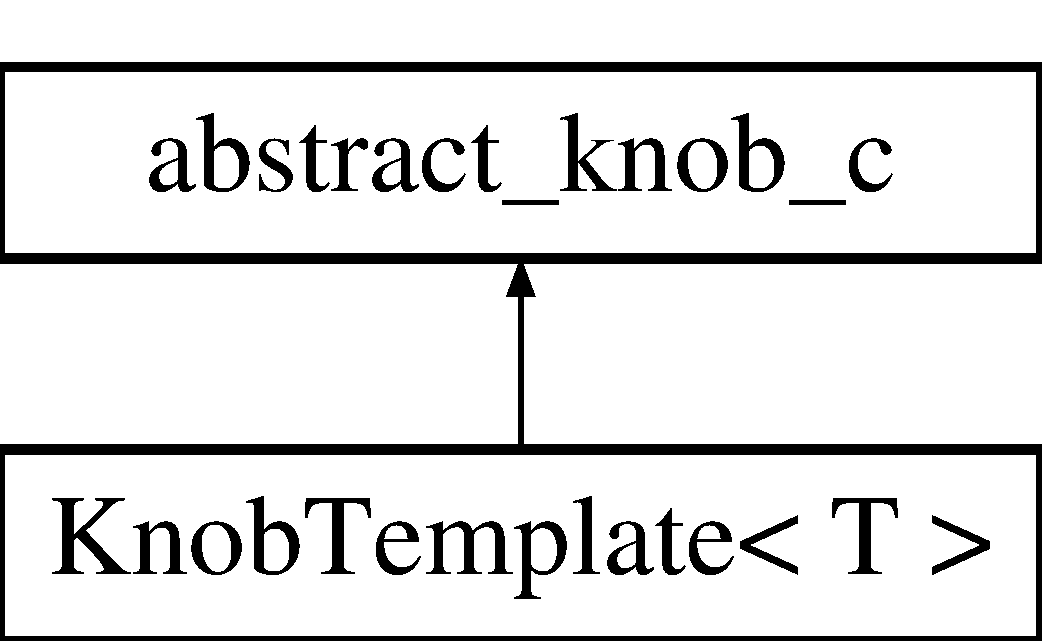
\includegraphics[height=2.000000cm]{classKnobTemplate}
\end{center}
\end{figure}
\subsection*{Public Member Functions}
\begin{DoxyCompactItemize}
\item 
\hyperlink{classKnobTemplate_aaddb7933b87960bb107b664c64b9be35}{KnobTemplate} ()
\item 
\hyperlink{classKnobTemplate_abbccdaab4475aa203cc72114e6c755c9}{KnobTemplate} (const string \&name, const T \&val, const string \&parentName=\char`\"{}\char`\"{})
\item 
\hyperlink{classKnobTemplate}{KnobTemplate}$<$ T $>$ \& \hyperlink{classKnobTemplate_a2ca50f6173b1b904310be277eb0bb4c1}{setValue} (const T \&val)
\item 
virtual void \hyperlink{classKnobTemplate_a56f3e765c947ac3e63f759d7b3188e42}{initFromString} (const string \&strVal)
\item 
const T \hyperlink{classKnobTemplate_a7191e4a940e968e7a1a41d606802300a}{getValue} () const 
\item 
\hyperlink{classKnobTemplate_aa23d5fa0b0f63756f03690d650bf697b}{operator T} () const 
\item 
virtual void \hyperlink{classKnobTemplate_af9a940a1d590ad63fdef381388935273}{display} (ostream \&os)
\item 
string \hyperlink{classKnobTemplate_aded197b0d716077801868dd111e7d083}{GetValueString} (void)
\end{DoxyCompactItemize}
\subsection*{Private Member Functions}
\begin{DoxyCompactItemize}
\item 
\hyperlink{classKnobTemplate_a9f2d6a9dec66f03aba4af96a23b038a0}{KnobTemplate} (const \hyperlink{classKnobTemplate}{KnobTemplate} \&rhs)
\item 
const \hyperlink{classKnobTemplate}{KnobTemplate} \& \hyperlink{classKnobTemplate_a8e6df8ed32887499f1d2bac4d46c079d}{operator=} (const \hyperlink{classKnobTemplate}{KnobTemplate} \&rhs)
\end{DoxyCompactItemize}
\subsection*{Private Attributes}
\begin{DoxyCompactItemize}
\item 
T \hyperlink{classKnobTemplate_a39c36d8924757ad7ef98e51eecadc033}{m\_\-value}
\end{DoxyCompactItemize}


\subsection{Detailed Description}
\subsubsection*{template$<$class T$>$ class KnobTemplate$<$ T $>$}

Knob template class with type T. 

\subsection{Constructor \& Destructor Documentation}
\hypertarget{classKnobTemplate_aaddb7933b87960bb107b664c64b9be35}{
\index{KnobTemplate@{KnobTemplate}!KnobTemplate@{KnobTemplate}}
\index{KnobTemplate@{KnobTemplate}!KnobTemplate@{KnobTemplate}}
\subsubsection[{KnobTemplate}]{\setlength{\rightskip}{0pt plus 5cm}template$<$class T$>$ {\bf KnobTemplate}$<$ T $>$::{\bf KnobTemplate} (
\begin{DoxyParamCaption}
{}
\end{DoxyParamCaption}
)\hspace{0.3cm}{\ttfamily  \mbox{[}inline\mbox{]}}}}
\label{classKnobTemplate_aaddb7933b87960bb107b664c64b9be35}
Constructor. \hypertarget{classKnobTemplate_abbccdaab4475aa203cc72114e6c755c9}{
\index{KnobTemplate@{KnobTemplate}!KnobTemplate@{KnobTemplate}}
\index{KnobTemplate@{KnobTemplate}!KnobTemplate@{KnobTemplate}}
\subsubsection[{KnobTemplate}]{\setlength{\rightskip}{0pt plus 5cm}template$<$class T$>$ {\bf KnobTemplate}$<$ T $>$::{\bf KnobTemplate} (
\begin{DoxyParamCaption}
\item[{const string \&}]{ name, }
\item[{const T \&}]{ val, }
\item[{const string \&}]{ parentName = {\ttfamily \char`\"{}\char`\"{}}}
\end{DoxyParamCaption}
)\hspace{0.3cm}{\ttfamily  \mbox{[}inline\mbox{]}}}}
\label{classKnobTemplate_abbccdaab4475aa203cc72114e6c755c9}
Constructor. 
\begin{DoxyParams}{Parameters}
\item[{\em name}]name of the knob \item[{\em val}]value of the knob \item[{\em parentName}]parent knob name \end{DoxyParams}
\hypertarget{classKnobTemplate_a9f2d6a9dec66f03aba4af96a23b038a0}{
\index{KnobTemplate@{KnobTemplate}!KnobTemplate@{KnobTemplate}}
\index{KnobTemplate@{KnobTemplate}!KnobTemplate@{KnobTemplate}}
\subsubsection[{KnobTemplate}]{\setlength{\rightskip}{0pt plus 5cm}template$<$class T$>$ {\bf KnobTemplate}$<$ T $>$::{\bf KnobTemplate} (
\begin{DoxyParamCaption}
\item[{const {\bf KnobTemplate}$<$ T $>$ \&}]{ rhs}
\end{DoxyParamCaption}
)\hspace{0.3cm}{\ttfamily  \mbox{[}private\mbox{]}}}}
\label{classKnobTemplate_a9f2d6a9dec66f03aba4af96a23b038a0}
Copy constructor. 

\subsection{Member Function Documentation}
\hypertarget{classKnobTemplate_af9a940a1d590ad63fdef381388935273}{
\index{KnobTemplate@{KnobTemplate}!display@{display}}
\index{display@{display}!KnobTemplate@{KnobTemplate}}
\subsubsection[{display}]{\setlength{\rightskip}{0pt plus 5cm}template$<$class T$>$ virtual void {\bf KnobTemplate}$<$ T $>$::display (
\begin{DoxyParamCaption}
\item[{ostream \&}]{ os}
\end{DoxyParamCaption}
)\hspace{0.3cm}{\ttfamily  \mbox{[}inline, virtual\mbox{]}}}}
\label{classKnobTemplate_af9a940a1d590ad63fdef381388935273}
Print knob name and its value. 

Reimplemented from \hyperlink{classabstract__knob__c_aaee4499a56d94f1831e7945274dfac8b}{abstract\_\-knob\_\-c}.

\hypertarget{classKnobTemplate_a7191e4a940e968e7a1a41d606802300a}{
\index{KnobTemplate@{KnobTemplate}!getValue@{getValue}}
\index{getValue@{getValue}!KnobTemplate@{KnobTemplate}}
\subsubsection[{getValue}]{\setlength{\rightskip}{0pt plus 5cm}template$<$class T$>$ const T {\bf KnobTemplate}$<$ T $>$::getValue (
\begin{DoxyParamCaption}
{}
\end{DoxyParamCaption}
) const\hspace{0.3cm}{\ttfamily  \mbox{[}inline\mbox{]}}}}
\label{classKnobTemplate_a7191e4a940e968e7a1a41d606802300a}
Get the value of the knob. \hypertarget{classKnobTemplate_aded197b0d716077801868dd111e7d083}{
\index{KnobTemplate@{KnobTemplate}!GetValueString@{GetValueString}}
\index{GetValueString@{GetValueString}!KnobTemplate@{KnobTemplate}}
\subsubsection[{GetValueString}]{\setlength{\rightskip}{0pt plus 5cm}template$<$class T$>$ string {\bf KnobTemplate}$<$ T $>$::GetValueString (
\begin{DoxyParamCaption}
\item[{void}]{}
\end{DoxyParamCaption}
)\hspace{0.3cm}{\ttfamily  \mbox{[}inline\mbox{]}}}}
\label{classKnobTemplate_aded197b0d716077801868dd111e7d083}
Get the value of the knob in string. \hypertarget{classKnobTemplate_a56f3e765c947ac3e63f759d7b3188e42}{
\index{KnobTemplate@{KnobTemplate}!initFromString@{initFromString}}
\index{initFromString@{initFromString}!KnobTemplate@{KnobTemplate}}
\subsubsection[{initFromString}]{\setlength{\rightskip}{0pt plus 5cm}template$<$class T$>$ virtual void {\bf KnobTemplate}$<$ T $>$::initFromString (
\begin{DoxyParamCaption}
\item[{const string \&}]{ strVal}
\end{DoxyParamCaption}
)\hspace{0.3cm}{\ttfamily  \mbox{[}inline, virtual\mbox{]}}}}
\label{classKnobTemplate_a56f3e765c947ac3e63f759d7b3188e42}
Initialize a knob from the string. 

Implements \hyperlink{classabstract__knob__c_ad69620dc8974d5c659c6a7828d460e28}{abstract\_\-knob\_\-c}.

\hypertarget{classKnobTemplate_aa23d5fa0b0f63756f03690d650bf697b}{
\index{KnobTemplate@{KnobTemplate}!operator T@{operator T}}
\index{operator T@{operator T}!KnobTemplate@{KnobTemplate}}
\subsubsection[{operator T}]{\setlength{\rightskip}{0pt plus 5cm}template$<$class T$>$ {\bf KnobTemplate}$<$ T $>$::operator T (
\begin{DoxyParamCaption}
{}
\end{DoxyParamCaption}
) const\hspace{0.3cm}{\ttfamily  \mbox{[}inline\mbox{]}}}}
\label{classKnobTemplate_aa23d5fa0b0f63756f03690d650bf697b}
Conversion operator (). Return the value of the knob. \hypertarget{classKnobTemplate_a8e6df8ed32887499f1d2bac4d46c079d}{
\index{KnobTemplate@{KnobTemplate}!operator=@{operator=}}
\index{operator=@{operator=}!KnobTemplate@{KnobTemplate}}
\subsubsection[{operator=}]{\setlength{\rightskip}{0pt plus 5cm}template$<$class T$>$ const {\bf KnobTemplate}\& {\bf KnobTemplate}$<$ T $>$::operator= (
\begin{DoxyParamCaption}
\item[{const {\bf KnobTemplate}$<$ T $>$ \&}]{ rhs}
\end{DoxyParamCaption}
)\hspace{0.3cm}{\ttfamily  \mbox{[}private\mbox{]}}}}
\label{classKnobTemplate_a8e6df8ed32887499f1d2bac4d46c079d}
Overidden operator =. \hypertarget{classKnobTemplate_a2ca50f6173b1b904310be277eb0bb4c1}{
\index{KnobTemplate@{KnobTemplate}!setValue@{setValue}}
\index{setValue@{setValue}!KnobTemplate@{KnobTemplate}}
\subsubsection[{setValue}]{\setlength{\rightskip}{0pt plus 5cm}template$<$class T$>$ {\bf KnobTemplate}$<$T$>$\& {\bf KnobTemplate}$<$ T $>$::setValue (
\begin{DoxyParamCaption}
\item[{const T \&}]{ val}
\end{DoxyParamCaption}
)\hspace{0.3cm}{\ttfamily  \mbox{[}inline\mbox{]}}}}
\label{classKnobTemplate_a2ca50f6173b1b904310be277eb0bb4c1}
Set the value of the knob. 

\subsection{Member Data Documentation}
\hypertarget{classKnobTemplate_a39c36d8924757ad7ef98e51eecadc033}{
\index{KnobTemplate@{KnobTemplate}!m\_\-value@{m\_\-value}}
\index{m\_\-value@{m\_\-value}!KnobTemplate@{KnobTemplate}}
\subsubsection[{m\_\-value}]{\setlength{\rightskip}{0pt plus 5cm}template$<$class T$>$ T {\bf KnobTemplate}$<$ T $>$::{\bf m\_\-value}\hspace{0.3cm}{\ttfamily  \mbox{[}private\mbox{]}}}}
\label{classKnobTemplate_a39c36d8924757ad7ef98e51eecadc033}
knob value 

The documentation for this class was generated from the following file:\begin{DoxyCompactItemize}
\item 
knob.h\end{DoxyCompactItemize}

\hypertarget{classKnobTemplate_3_01string_01_4}{
\section{KnobTemplate$<$ string $>$ Class Template Reference}
\label{classKnobTemplate_3_01string_01_4}\index{KnobTemplate$<$ string $>$@{KnobTemplate$<$ string $>$}}
}


string type knob class  




{\ttfamily \#include $<$knob.h$>$}

Inheritance diagram for KnobTemplate$<$ string $>$:\begin{figure}[H]
\begin{center}
\leavevmode
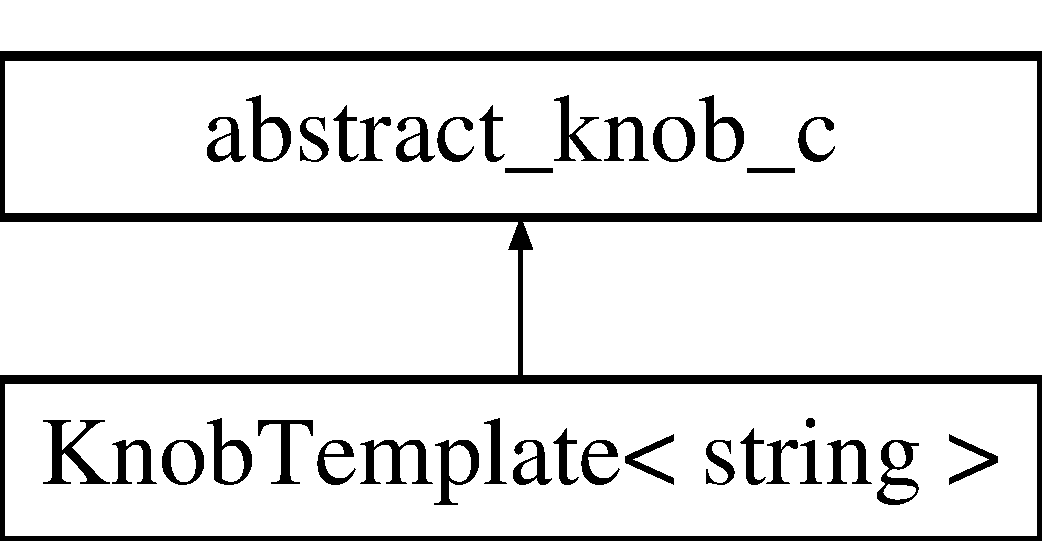
\includegraphics[height=2.000000cm]{classKnobTemplate_3_01string_01_4}
\end{center}
\end{figure}
\subsection*{Public Member Functions}
\begin{DoxyCompactItemize}
\item 
\hyperlink{classKnobTemplate_3_01string_01_4_a6d71f31045ce02f191142d3fac09b96e}{KnobTemplate} (const string \&name, const string \&val, const string \&parentName=\char`\"{}\char`\"{})
\item 
\hyperlink{classKnobTemplate}{KnobTemplate}$<$ string $>$ \& \hyperlink{classKnobTemplate_3_01string_01_4_ae5810b244d49ed723f973d9cab1f608f}{setValue} (const string \&val)
\item 
virtual void \hyperlink{classKnobTemplate_3_01string_01_4_ae8fc9c5a7ed9be681b059083338902f7}{initFromString} (const string \&strVal)
\item 
const string \hyperlink{classKnobTemplate_3_01string_01_4_aeedbeeef8d6b8b4d7d8f7b230b714633}{getValue} () const 
\item 
\hyperlink{classKnobTemplate_3_01string_01_4_a702d6aa199956f7ce635da4069f1dbd9}{operator string} () const 
\item 
\hyperlink{classKnobTemplate_3_01string_01_4_ae578d85aaa47c81763db05dda5de61d5}{operator bool} () const 
\item 
virtual void \hyperlink{classKnobTemplate_3_01string_01_4_aee99cda916cd052abaf36957bf6e3a03}{display} (ostream \&os)
\end{DoxyCompactItemize}
\subsection*{Private Member Functions}
\begin{DoxyCompactItemize}
\item 
\hyperlink{classKnobTemplate_3_01string_01_4_a15edde26af3fe3516ef60301368b5d31}{KnobTemplate} (const \hyperlink{classKnobTemplate}{KnobTemplate} \&rhs)
\item 
const \hyperlink{classKnobTemplate}{KnobTemplate} \& \hyperlink{classKnobTemplate_3_01string_01_4_a9c99e9b3292d1df82c49b9b61159f0f7}{operator=} (const \hyperlink{classKnobTemplate}{KnobTemplate} \&rhs)
\end{DoxyCompactItemize}
\subsection*{Private Attributes}
\begin{DoxyCompactItemize}
\item 
string \hyperlink{classKnobTemplate_3_01string_01_4_a109a8b0e27146550576ef4e5a7babeac}{m\_\-value}
\end{DoxyCompactItemize}


\subsection{Detailed Description}
\subsubsection*{template$<$$>$ class KnobTemplate$<$ string $>$}

string type knob class 

\subsection{Constructor \& Destructor Documentation}
\hypertarget{classKnobTemplate_3_01string_01_4_a6d71f31045ce02f191142d3fac09b96e}{
\index{KnobTemplate$<$ string $>$@{KnobTemplate$<$ string $>$}!KnobTemplate@{KnobTemplate}}
\index{KnobTemplate@{KnobTemplate}!KnobTemplate< string >@{KnobTemplate$<$ string $>$}}
\subsubsection[{KnobTemplate}]{\setlength{\rightskip}{0pt plus 5cm}{\bf KnobTemplate}$<$ string $>$::{\bf KnobTemplate} (
\begin{DoxyParamCaption}
\item[{const string \&}]{ name, }
\item[{const string \&}]{ val, }
\item[{const string \&}]{ parentName = {\ttfamily \char`\"{}\char`\"{}}}
\end{DoxyParamCaption}
)\hspace{0.3cm}{\ttfamily  \mbox{[}inline\mbox{]}}}}
\label{classKnobTemplate_3_01string_01_4_a6d71f31045ce02f191142d3fac09b96e}
Constructor. 
\begin{DoxyParams}{Parameters}
\item[{\em name}]knob name \item[{\em val}]knob value \item[{\em parentName}]the name of parent knob \end{DoxyParams}
\hypertarget{classKnobTemplate_3_01string_01_4_a15edde26af3fe3516ef60301368b5d31}{
\index{KnobTemplate$<$ string $>$@{KnobTemplate$<$ string $>$}!KnobTemplate@{KnobTemplate}}
\index{KnobTemplate@{KnobTemplate}!KnobTemplate< string >@{KnobTemplate$<$ string $>$}}
\subsubsection[{KnobTemplate}]{\setlength{\rightskip}{0pt plus 5cm}{\bf KnobTemplate}$<$ string $>$::{\bf KnobTemplate} (
\begin{DoxyParamCaption}
\item[{const {\bf KnobTemplate}$<$ string $>$ \&}]{ rhs}
\end{DoxyParamCaption}
)\hspace{0.3cm}{\ttfamily  \mbox{[}private\mbox{]}}}}
\label{classKnobTemplate_3_01string_01_4_a15edde26af3fe3516ef60301368b5d31}
Copy constructor. 

\subsection{Member Function Documentation}
\hypertarget{classKnobTemplate_3_01string_01_4_aee99cda916cd052abaf36957bf6e3a03}{
\index{KnobTemplate$<$ string $>$@{KnobTemplate$<$ string $>$}!display@{display}}
\index{display@{display}!KnobTemplate< string >@{KnobTemplate$<$ string $>$}}
\subsubsection[{display}]{\setlength{\rightskip}{0pt plus 5cm}virtual void {\bf KnobTemplate}$<$ string $>$::display (
\begin{DoxyParamCaption}
\item[{ostream \&}]{ os}
\end{DoxyParamCaption}
)\hspace{0.3cm}{\ttfamily  \mbox{[}inline, virtual\mbox{]}}}}
\label{classKnobTemplate_3_01string_01_4_aee99cda916cd052abaf36957bf6e3a03}
Print the name of a knob and its value. 

Reimplemented from \hyperlink{classabstract__knob__c_aaee4499a56d94f1831e7945274dfac8b}{abstract\_\-knob\_\-c}.

\hypertarget{classKnobTemplate_3_01string_01_4_aeedbeeef8d6b8b4d7d8f7b230b714633}{
\index{KnobTemplate$<$ string $>$@{KnobTemplate$<$ string $>$}!getValue@{getValue}}
\index{getValue@{getValue}!KnobTemplate< string >@{KnobTemplate$<$ string $>$}}
\subsubsection[{getValue}]{\setlength{\rightskip}{0pt plus 5cm}const string {\bf KnobTemplate}$<$ string $>$::getValue (
\begin{DoxyParamCaption}
{}
\end{DoxyParamCaption}
) const\hspace{0.3cm}{\ttfamily  \mbox{[}inline\mbox{]}}}}
\label{classKnobTemplate_3_01string_01_4_aeedbeeef8d6b8b4d7d8f7b230b714633}
Get the value of the knob. \hypertarget{classKnobTemplate_3_01string_01_4_ae8fc9c5a7ed9be681b059083338902f7}{
\index{KnobTemplate$<$ string $>$@{KnobTemplate$<$ string $>$}!initFromString@{initFromString}}
\index{initFromString@{initFromString}!KnobTemplate< string >@{KnobTemplate$<$ string $>$}}
\subsubsection[{initFromString}]{\setlength{\rightskip}{0pt plus 5cm}virtual void {\bf KnobTemplate}$<$ string $>$::initFromString (
\begin{DoxyParamCaption}
\item[{const string \&}]{ strVal}
\end{DoxyParamCaption}
)\hspace{0.3cm}{\ttfamily  \mbox{[}inline, virtual\mbox{]}}}}
\label{classKnobTemplate_3_01string_01_4_ae8fc9c5a7ed9be681b059083338902f7}
Initialize a knob from the string. 

Implements \hyperlink{classabstract__knob__c_ad69620dc8974d5c659c6a7828d460e28}{abstract\_\-knob\_\-c}.

\hypertarget{classKnobTemplate_3_01string_01_4_ae578d85aaa47c81763db05dda5de61d5}{
\index{KnobTemplate$<$ string $>$@{KnobTemplate$<$ string $>$}!operator bool@{operator bool}}
\index{operator bool@{operator bool}!KnobTemplate< string >@{KnobTemplate$<$ string $>$}}
\subsubsection[{operator bool}]{\setlength{\rightskip}{0pt plus 5cm}{\bf KnobTemplate}$<$ string $>$::operator bool (
\begin{DoxyParamCaption}
{}
\end{DoxyParamCaption}
) const\hspace{0.3cm}{\ttfamily  \mbox{[}inline\mbox{]}}}}
\label{classKnobTemplate_3_01string_01_4_ae578d85aaa47c81763db05dda5de61d5}
Conversion oeprator to bool. \hypertarget{classKnobTemplate_3_01string_01_4_a702d6aa199956f7ce635da4069f1dbd9}{
\index{KnobTemplate$<$ string $>$@{KnobTemplate$<$ string $>$}!operator string@{operator string}}
\index{operator string@{operator string}!KnobTemplate< string >@{KnobTemplate$<$ string $>$}}
\subsubsection[{operator string}]{\setlength{\rightskip}{0pt plus 5cm}{\bf KnobTemplate}$<$ string $>$::operator string (
\begin{DoxyParamCaption}
{}
\end{DoxyParamCaption}
) const\hspace{0.3cm}{\ttfamily  \mbox{[}inline\mbox{]}}}}
\label{classKnobTemplate_3_01string_01_4_a702d6aa199956f7ce635da4069f1dbd9}
Conversion operator to string. \hypertarget{classKnobTemplate_3_01string_01_4_a9c99e9b3292d1df82c49b9b61159f0f7}{
\index{KnobTemplate$<$ string $>$@{KnobTemplate$<$ string $>$}!operator=@{operator=}}
\index{operator=@{operator=}!KnobTemplate< string >@{KnobTemplate$<$ string $>$}}
\subsubsection[{operator=}]{\setlength{\rightskip}{0pt plus 5cm}const {\bf KnobTemplate}\& {\bf KnobTemplate}$<$ string $>$::operator= (
\begin{DoxyParamCaption}
\item[{const {\bf KnobTemplate}$<$ string $>$ \&}]{ rhs}
\end{DoxyParamCaption}
)\hspace{0.3cm}{\ttfamily  \mbox{[}private\mbox{]}}}}
\label{classKnobTemplate_3_01string_01_4_a9c99e9b3292d1df82c49b9b61159f0f7}
Overridden operator = \hypertarget{classKnobTemplate_3_01string_01_4_ae5810b244d49ed723f973d9cab1f608f}{
\index{KnobTemplate$<$ string $>$@{KnobTemplate$<$ string $>$}!setValue@{setValue}}
\index{setValue@{setValue}!KnobTemplate< string >@{KnobTemplate$<$ string $>$}}
\subsubsection[{setValue}]{\setlength{\rightskip}{0pt plus 5cm}{\bf KnobTemplate}$<$string$>$\& {\bf KnobTemplate}$<$ string $>$::setValue (
\begin{DoxyParamCaption}
\item[{const string \&}]{ val}
\end{DoxyParamCaption}
)\hspace{0.3cm}{\ttfamily  \mbox{[}inline\mbox{]}}}}
\label{classKnobTemplate_3_01string_01_4_ae5810b244d49ed723f973d9cab1f608f}
Set value of the knob. 

\subsection{Member Data Documentation}
\hypertarget{classKnobTemplate_3_01string_01_4_a109a8b0e27146550576ef4e5a7babeac}{
\index{KnobTemplate$<$ string $>$@{KnobTemplate$<$ string $>$}!m\_\-value@{m\_\-value}}
\index{m\_\-value@{m\_\-value}!KnobTemplate< string >@{KnobTemplate$<$ string $>$}}
\subsubsection[{m\_\-value}]{\setlength{\rightskip}{0pt plus 5cm}string {\bf KnobTemplate}$<$ string $>$::{\bf m\_\-value}\hspace{0.3cm}{\ttfamily  \mbox{[}private\mbox{]}}}}
\label{classKnobTemplate_3_01string_01_4_a109a8b0e27146550576ef4e5a7babeac}
knob value 

The documentation for this class was generated from the following file:\begin{DoxyCompactItemize}
\item 
knob.h\end{DoxyCompactItemize}

\hypertarget{classl2__coupled__local__c}{
\section{l2\_\-coupled\_\-local\_\-c Class Reference}
\label{classl2__coupled__local__c}\index{l2\_\-coupled\_\-local\_\-c@{l2\_\-coupled\_\-local\_\-c}}
}


2-\/Level, Local architecture (Intel Core 2)  




{\ttfamily \#include $<$memory.h$>$}

Inheritance diagram for l2\_\-coupled\_\-local\_\-c:\begin{figure}[H]
\begin{center}
\leavevmode
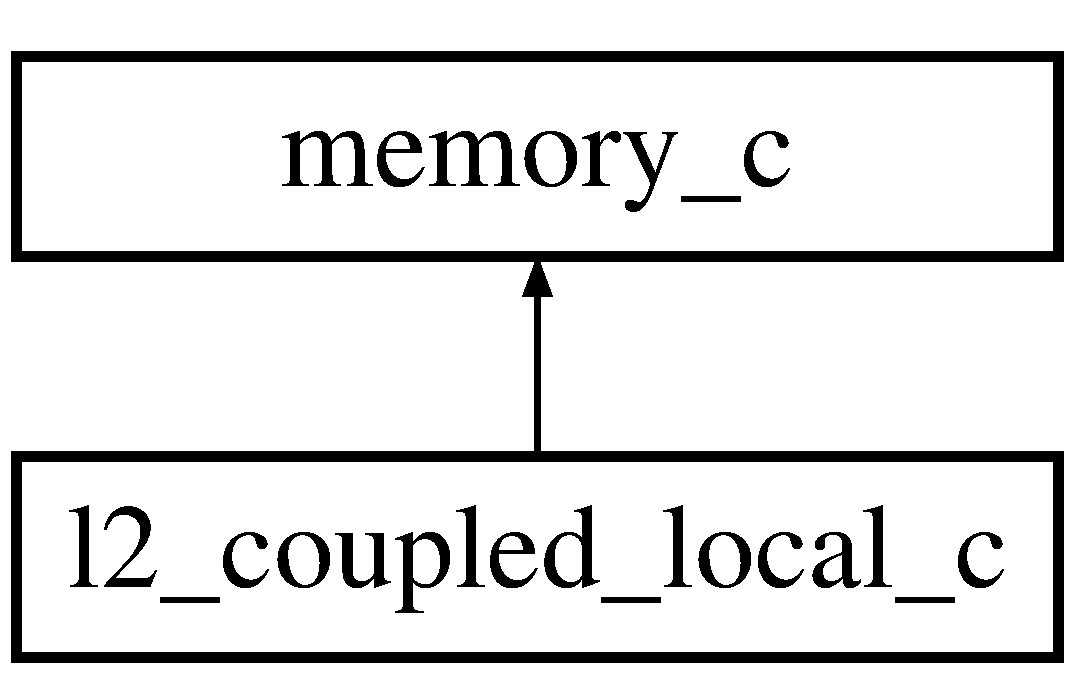
\includegraphics[height=2.000000cm]{classl2__coupled__local__c}
\end{center}
\end{figure}
\subsection*{Public Member Functions}
\begin{DoxyCompactItemize}
\item 
\hyperlink{classl2__coupled__local__c_ad323f078614dcc1ca6ee5329addf7a44}{l2\_\-coupled\_\-local\_\-c} (\hyperlink{classmacsim__c}{macsim\_\-c} $\ast$simBase)
\item 
\hyperlink{classl2__coupled__local__c_a721a9db728856d12ef03549e561d57ca}{$\sim$l2\_\-coupled\_\-local\_\-c} ()
\end{DoxyCompactItemize}
\subsection*{Private Member Functions}
\begin{DoxyCompactItemize}
\item 
void \hyperlink{classl2__coupled__local__c_a4f3ca72f4a2ee33fa7f8b97b21e72364}{set\_\-cache\_\-id} (\hyperlink{structmem__req__s}{mem\_\-req\_\-s} $\ast$req)
\end{DoxyCompactItemize}


\subsection{Detailed Description}
2-\/Level, Local architecture (Intel Core 2) 

\subsection{Constructor \& Destructor Documentation}
\hypertarget{classl2__coupled__local__c_ad323f078614dcc1ca6ee5329addf7a44}{
\index{l2\_\-coupled\_\-local\_\-c@{l2\_\-coupled\_\-local\_\-c}!l2\_\-coupled\_\-local\_\-c@{l2\_\-coupled\_\-local\_\-c}}
\index{l2\_\-coupled\_\-local\_\-c@{l2\_\-coupled\_\-local\_\-c}!l2_coupled_local_c@{l2\_\-coupled\_\-local\_\-c}}
\subsubsection[{l2\_\-coupled\_\-local\_\-c}]{\setlength{\rightskip}{0pt plus 5cm}l2\_\-coupled\_\-local\_\-c::l2\_\-coupled\_\-local\_\-c (
\begin{DoxyParamCaption}
\item[{{\bf macsim\_\-c} $\ast$}]{ simBase}
\end{DoxyParamCaption}
)}}
\label{classl2__coupled__local__c_ad323f078614dcc1ca6ee5329addf7a44}
Constructor \hypertarget{classl2__coupled__local__c_a721a9db728856d12ef03549e561d57ca}{
\index{l2\_\-coupled\_\-local\_\-c@{l2\_\-coupled\_\-local\_\-c}!$\sim$l2\_\-coupled\_\-local\_\-c@{$\sim$l2\_\-coupled\_\-local\_\-c}}
\index{$\sim$l2\_\-coupled\_\-local\_\-c@{$\sim$l2\_\-coupled\_\-local\_\-c}!l2_coupled_local_c@{l2\_\-coupled\_\-local\_\-c}}
\subsubsection[{$\sim$l2\_\-coupled\_\-local\_\-c}]{\setlength{\rightskip}{0pt plus 5cm}l2\_\-coupled\_\-local\_\-c::$\sim$l2\_\-coupled\_\-local\_\-c (
\begin{DoxyParamCaption}
{}
\end{DoxyParamCaption}
)}}
\label{classl2__coupled__local__c_a721a9db728856d12ef03549e561d57ca}
Destructor 

\subsection{Member Function Documentation}
\hypertarget{classl2__coupled__local__c_a4f3ca72f4a2ee33fa7f8b97b21e72364}{
\index{l2\_\-coupled\_\-local\_\-c@{l2\_\-coupled\_\-local\_\-c}!set\_\-cache\_\-id@{set\_\-cache\_\-id}}
\index{set\_\-cache\_\-id@{set\_\-cache\_\-id}!l2_coupled_local_c@{l2\_\-coupled\_\-local\_\-c}}
\subsubsection[{set\_\-cache\_\-id}]{\setlength{\rightskip}{0pt plus 5cm}void l2\_\-coupled\_\-local\_\-c::set\_\-cache\_\-id (
\begin{DoxyParamCaption}
\item[{{\bf mem\_\-req\_\-s} $\ast$}]{ req}
\end{DoxyParamCaption}
)\hspace{0.3cm}{\ttfamily  \mbox{[}private, virtual\mbox{]}}}}
\label{classl2__coupled__local__c_a4f3ca72f4a2ee33fa7f8b97b21e72364}
Set the level of each cache level 

Reimplemented from \hyperlink{classmemory__c_aa15a04b3d5bb8e6ab0b7274b9c50a319}{memory\_\-c}.



The documentation for this class was generated from the following files:\begin{DoxyCompactItemize}
\item 
memory.h\item 
memory.cc\end{DoxyCompactItemize}

\hypertarget{classl2__decoupled__local__c}{
\section{l2\_\-decoupled\_\-local\_\-c Class Reference}
\label{classl2__decoupled__local__c}\index{l2\_\-decoupled\_\-local\_\-c@{l2\_\-decoupled\_\-local\_\-c}}
}


2-\/Level, L2 is accessed locally (Intel Core 2)  




{\ttfamily \#include $<$memory.h$>$}

Inheritance diagram for l2\_\-decoupled\_\-local\_\-c:\begin{figure}[H]
\begin{center}
\leavevmode
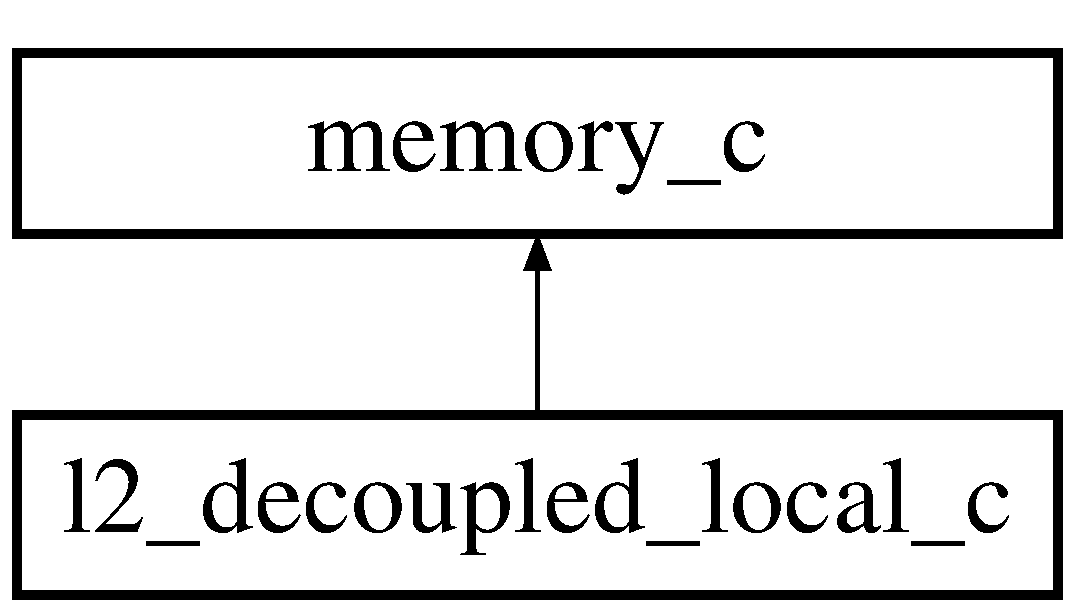
\includegraphics[height=2.000000cm]{classl2__decoupled__local__c}
\end{center}
\end{figure}
\subsection*{Public Member Functions}
\begin{DoxyCompactItemize}
\item 
\hyperlink{classl2__decoupled__local__c_a06f0e007f417ffe7c3fe01e79d30d4f3}{l2\_\-decoupled\_\-local\_\-c} (\hyperlink{classmacsim__c}{macsim\_\-c} $\ast$simBase)
\item 
\hyperlink{classl2__decoupled__local__c_a7bfff94c2cb1ff669b3bf352208b8333}{$\sim$l2\_\-decoupled\_\-local\_\-c} ()
\end{DoxyCompactItemize}
\subsection*{Private Member Functions}
\begin{DoxyCompactItemize}
\item 
void \hyperlink{classl2__decoupled__local__c_a4c319b02982447d98079bf6649fa5c15}{set\_\-cache\_\-id} (\hyperlink{structmem__req__s}{mem\_\-req\_\-s} $\ast$req)
\end{DoxyCompactItemize}


\subsection{Detailed Description}
2-\/Level, L2 is accessed locally (Intel Core 2) 

\subsection{Constructor \& Destructor Documentation}
\hypertarget{classl2__decoupled__local__c_a06f0e007f417ffe7c3fe01e79d30d4f3}{
\index{l2\_\-decoupled\_\-local\_\-c@{l2\_\-decoupled\_\-local\_\-c}!l2\_\-decoupled\_\-local\_\-c@{l2\_\-decoupled\_\-local\_\-c}}
\index{l2\_\-decoupled\_\-local\_\-c@{l2\_\-decoupled\_\-local\_\-c}!l2_decoupled_local_c@{l2\_\-decoupled\_\-local\_\-c}}
\subsubsection[{l2\_\-decoupled\_\-local\_\-c}]{\setlength{\rightskip}{0pt plus 5cm}l2\_\-decoupled\_\-local\_\-c::l2\_\-decoupled\_\-local\_\-c (
\begin{DoxyParamCaption}
\item[{{\bf macsim\_\-c} $\ast$}]{ simBase}
\end{DoxyParamCaption}
)}}
\label{classl2__decoupled__local__c_a06f0e007f417ffe7c3fe01e79d30d4f3}
Constructor \hypertarget{classl2__decoupled__local__c_a7bfff94c2cb1ff669b3bf352208b8333}{
\index{l2\_\-decoupled\_\-local\_\-c@{l2\_\-decoupled\_\-local\_\-c}!$\sim$l2\_\-decoupled\_\-local\_\-c@{$\sim$l2\_\-decoupled\_\-local\_\-c}}
\index{$\sim$l2\_\-decoupled\_\-local\_\-c@{$\sim$l2\_\-decoupled\_\-local\_\-c}!l2_decoupled_local_c@{l2\_\-decoupled\_\-local\_\-c}}
\subsubsection[{$\sim$l2\_\-decoupled\_\-local\_\-c}]{\setlength{\rightskip}{0pt plus 5cm}l2\_\-decoupled\_\-local\_\-c::$\sim$l2\_\-decoupled\_\-local\_\-c (
\begin{DoxyParamCaption}
{}
\end{DoxyParamCaption}
)}}
\label{classl2__decoupled__local__c_a7bfff94c2cb1ff669b3bf352208b8333}
Destructor 

\subsection{Member Function Documentation}
\hypertarget{classl2__decoupled__local__c_a4c319b02982447d98079bf6649fa5c15}{
\index{l2\_\-decoupled\_\-local\_\-c@{l2\_\-decoupled\_\-local\_\-c}!set\_\-cache\_\-id@{set\_\-cache\_\-id}}
\index{set\_\-cache\_\-id@{set\_\-cache\_\-id}!l2_decoupled_local_c@{l2\_\-decoupled\_\-local\_\-c}}
\subsubsection[{set\_\-cache\_\-id}]{\setlength{\rightskip}{0pt plus 5cm}void l2\_\-decoupled\_\-local\_\-c::set\_\-cache\_\-id (
\begin{DoxyParamCaption}
\item[{{\bf mem\_\-req\_\-s} $\ast$}]{ req}
\end{DoxyParamCaption}
)\hspace{0.3cm}{\ttfamily  \mbox{[}private, virtual\mbox{]}}}}
\label{classl2__decoupled__local__c_a4c319b02982447d98079bf6649fa5c15}
Set the level of each cache level 

Reimplemented from \hyperlink{classmemory__c_aa15a04b3d5bb8e6ab0b7274b9c50a319}{memory\_\-c}.



The documentation for this class was generated from the following files:\begin{DoxyCompactItemize}
\item 
memory.h\item 
memory.cc\end{DoxyCompactItemize}

\hypertarget{classl2__decoupled__network__c}{
\section{l2\_\-decoupled\_\-network\_\-c Class Reference}
\label{classl2__decoupled__network__c}\index{l2\_\-decoupled\_\-network\_\-c@{l2\_\-decoupled\_\-network\_\-c}}
}


2-\/Level, L2 is accessed via NoC (NVIDIA Fermi)  




{\ttfamily \#include $<$memory.h$>$}

Inheritance diagram for l2\_\-decoupled\_\-network\_\-c:\begin{figure}[H]
\begin{center}
\leavevmode
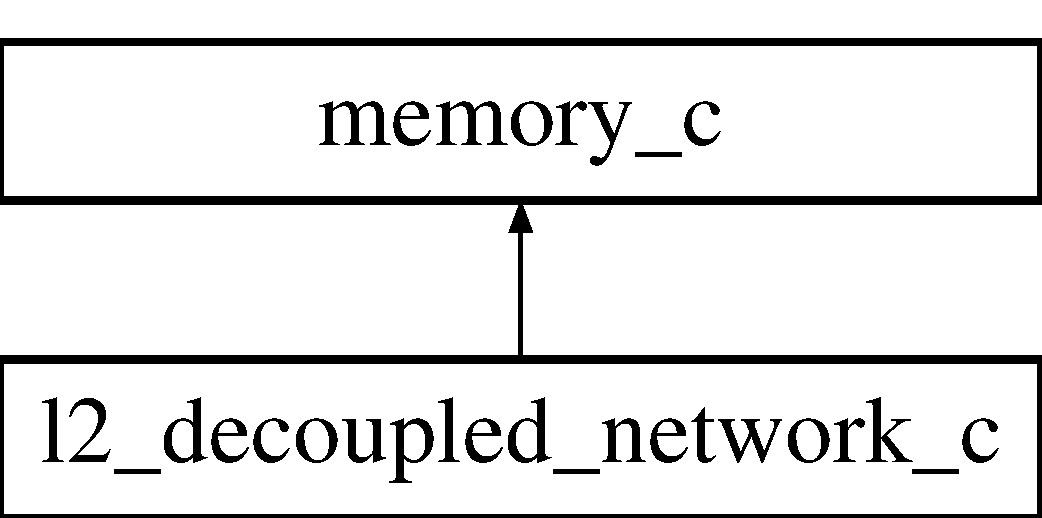
\includegraphics[height=2.000000cm]{classl2__decoupled__network__c}
\end{center}
\end{figure}
\subsection*{Public Member Functions}
\begin{DoxyCompactItemize}
\item 
\hyperlink{classl2__decoupled__network__c_a702ce99305d9252cc41167a69ac5e54b}{l2\_\-decoupled\_\-network\_\-c} (\hyperlink{classmacsim__c}{macsim\_\-c} $\ast$simBase)
\item 
\hyperlink{classl2__decoupled__network__c_a2fc1a52406c46fee438c755912ae2878}{$\sim$l2\_\-decoupled\_\-network\_\-c} ()
\end{DoxyCompactItemize}
\subsection*{Private Member Functions}
\begin{DoxyCompactItemize}
\item 
void \hyperlink{classl2__decoupled__network__c_aea63c8492607041d4d3ab90c8fa2961e}{set\_\-cache\_\-id} (\hyperlink{structmem__req__s}{mem\_\-req\_\-s} $\ast$req)
\end{DoxyCompactItemize}


\subsection{Detailed Description}
2-\/Level, L2 is accessed via NoC (NVIDIA Fermi) 

\subsection{Constructor \& Destructor Documentation}
\hypertarget{classl2__decoupled__network__c_a702ce99305d9252cc41167a69ac5e54b}{
\index{l2\_\-decoupled\_\-network\_\-c@{l2\_\-decoupled\_\-network\_\-c}!l2\_\-decoupled\_\-network\_\-c@{l2\_\-decoupled\_\-network\_\-c}}
\index{l2\_\-decoupled\_\-network\_\-c@{l2\_\-decoupled\_\-network\_\-c}!l2_decoupled_network_c@{l2\_\-decoupled\_\-network\_\-c}}
\subsubsection[{l2\_\-decoupled\_\-network\_\-c}]{\setlength{\rightskip}{0pt plus 5cm}l2\_\-decoupled\_\-network\_\-c::l2\_\-decoupled\_\-network\_\-c (
\begin{DoxyParamCaption}
\item[{{\bf macsim\_\-c} $\ast$}]{ simBase}
\end{DoxyParamCaption}
)}}
\label{classl2__decoupled__network__c_a702ce99305d9252cc41167a69ac5e54b}
Constructor \hypertarget{classl2__decoupled__network__c_a2fc1a52406c46fee438c755912ae2878}{
\index{l2\_\-decoupled\_\-network\_\-c@{l2\_\-decoupled\_\-network\_\-c}!$\sim$l2\_\-decoupled\_\-network\_\-c@{$\sim$l2\_\-decoupled\_\-network\_\-c}}
\index{$\sim$l2\_\-decoupled\_\-network\_\-c@{$\sim$l2\_\-decoupled\_\-network\_\-c}!l2_decoupled_network_c@{l2\_\-decoupled\_\-network\_\-c}}
\subsubsection[{$\sim$l2\_\-decoupled\_\-network\_\-c}]{\setlength{\rightskip}{0pt plus 5cm}l2\_\-decoupled\_\-network\_\-c::$\sim$l2\_\-decoupled\_\-network\_\-c (
\begin{DoxyParamCaption}
{}
\end{DoxyParamCaption}
)}}
\label{classl2__decoupled__network__c_a2fc1a52406c46fee438c755912ae2878}
Destructor 

\subsection{Member Function Documentation}
\hypertarget{classl2__decoupled__network__c_aea63c8492607041d4d3ab90c8fa2961e}{
\index{l2\_\-decoupled\_\-network\_\-c@{l2\_\-decoupled\_\-network\_\-c}!set\_\-cache\_\-id@{set\_\-cache\_\-id}}
\index{set\_\-cache\_\-id@{set\_\-cache\_\-id}!l2_decoupled_network_c@{l2\_\-decoupled\_\-network\_\-c}}
\subsubsection[{set\_\-cache\_\-id}]{\setlength{\rightskip}{0pt plus 5cm}void l2\_\-decoupled\_\-network\_\-c::set\_\-cache\_\-id (
\begin{DoxyParamCaption}
\item[{{\bf mem\_\-req\_\-s} $\ast$}]{ req}
\end{DoxyParamCaption}
)\hspace{0.3cm}{\ttfamily  \mbox{[}private, virtual\mbox{]}}}}
\label{classl2__decoupled__network__c_aea63c8492607041d4d3ab90c8fa2961e}
Set the level of each cache level 

Reimplemented from \hyperlink{classmemory__c_aa15a04b3d5bb8e6ab0b7274b9c50a319}{memory\_\-c}.



The documentation for this class was generated from the following files:\begin{DoxyCompactItemize}
\item 
memory.h\item 
memory.cc\end{DoxyCompactItemize}

\hypertarget{classl3__coupled__network__c}{
\section{l3\_\-coupled\_\-network\_\-c Class Reference}
\label{classl3__coupled__network__c}\index{l3\_\-coupled\_\-network\_\-c@{l3\_\-coupled\_\-network\_\-c}}
}


3-\/Level, Coupled architecture (Intel Sandy Bridge)  




{\ttfamily \#include $<$memory.h$>$}

Inheritance diagram for l3\_\-coupled\_\-network\_\-c:\begin{figure}[H]
\begin{center}
\leavevmode
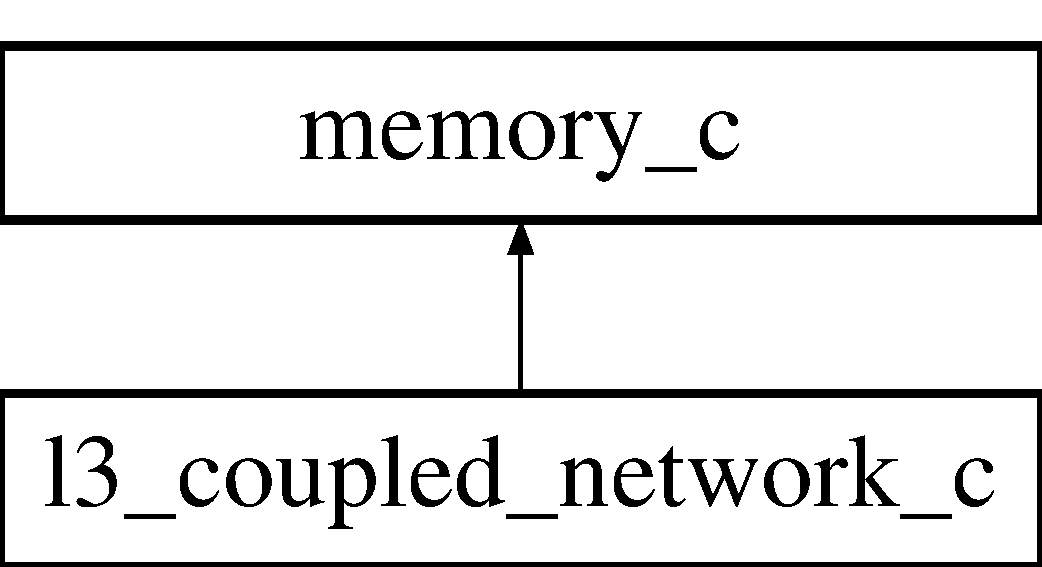
\includegraphics[height=2.000000cm]{classl3__coupled__network__c}
\end{center}
\end{figure}
\subsection*{Public Member Functions}
\begin{DoxyCompactItemize}
\item 
\hyperlink{classl3__coupled__network__c_acce488887d4a317807384144b34deeb6}{l3\_\-coupled\_\-network\_\-c} (\hyperlink{classmacsim__c}{macsim\_\-c} $\ast$simBase)
\item 
\hyperlink{classl3__coupled__network__c_a31117e8df70c5019f948cdf7416e2348}{$\sim$l3\_\-coupled\_\-network\_\-c} ()
\end{DoxyCompactItemize}


\subsection{Detailed Description}
3-\/Level, Coupled architecture (Intel Sandy Bridge) 

\subsection{Constructor \& Destructor Documentation}
\hypertarget{classl3__coupled__network__c_acce488887d4a317807384144b34deeb6}{
\index{l3\_\-coupled\_\-network\_\-c@{l3\_\-coupled\_\-network\_\-c}!l3\_\-coupled\_\-network\_\-c@{l3\_\-coupled\_\-network\_\-c}}
\index{l3\_\-coupled\_\-network\_\-c@{l3\_\-coupled\_\-network\_\-c}!l3_coupled_network_c@{l3\_\-coupled\_\-network\_\-c}}
\subsubsection[{l3\_\-coupled\_\-network\_\-c}]{\setlength{\rightskip}{0pt plus 5cm}l3\_\-coupled\_\-network\_\-c::l3\_\-coupled\_\-network\_\-c (
\begin{DoxyParamCaption}
\item[{{\bf macsim\_\-c} $\ast$}]{ simBase}
\end{DoxyParamCaption}
)}}
\label{classl3__coupled__network__c_acce488887d4a317807384144b34deeb6}
constructor \hypertarget{classl3__coupled__network__c_a31117e8df70c5019f948cdf7416e2348}{
\index{l3\_\-coupled\_\-network\_\-c@{l3\_\-coupled\_\-network\_\-c}!$\sim$l3\_\-coupled\_\-network\_\-c@{$\sim$l3\_\-coupled\_\-network\_\-c}}
\index{$\sim$l3\_\-coupled\_\-network\_\-c@{$\sim$l3\_\-coupled\_\-network\_\-c}!l3_coupled_network_c@{l3\_\-coupled\_\-network\_\-c}}
\subsubsection[{$\sim$l3\_\-coupled\_\-network\_\-c}]{\setlength{\rightskip}{0pt plus 5cm}l3\_\-coupled\_\-network\_\-c::$\sim$l3\_\-coupled\_\-network\_\-c (
\begin{DoxyParamCaption}
{}
\end{DoxyParamCaption}
)}}
\label{classl3__coupled__network__c_a31117e8df70c5019f948cdf7416e2348}
Destructor 

The documentation for this class was generated from the following files:\begin{DoxyCompactItemize}
\item 
memory.h\item 
memory.cc\end{DoxyCompactItemize}

\hypertarget{classl3__decoupled__network__c}{
\section{l3\_\-decoupled\_\-network\_\-c Class Reference}
\label{classl3__decoupled__network__c}\index{l3\_\-decoupled\_\-network\_\-c@{l3\_\-decoupled\_\-network\_\-c}}
}


3-\/Level, Decoupled architecture (2D topology)  




{\ttfamily \#include $<$memory.h$>$}

Inheritance diagram for l3\_\-decoupled\_\-network\_\-c:\begin{figure}[H]
\begin{center}
\leavevmode
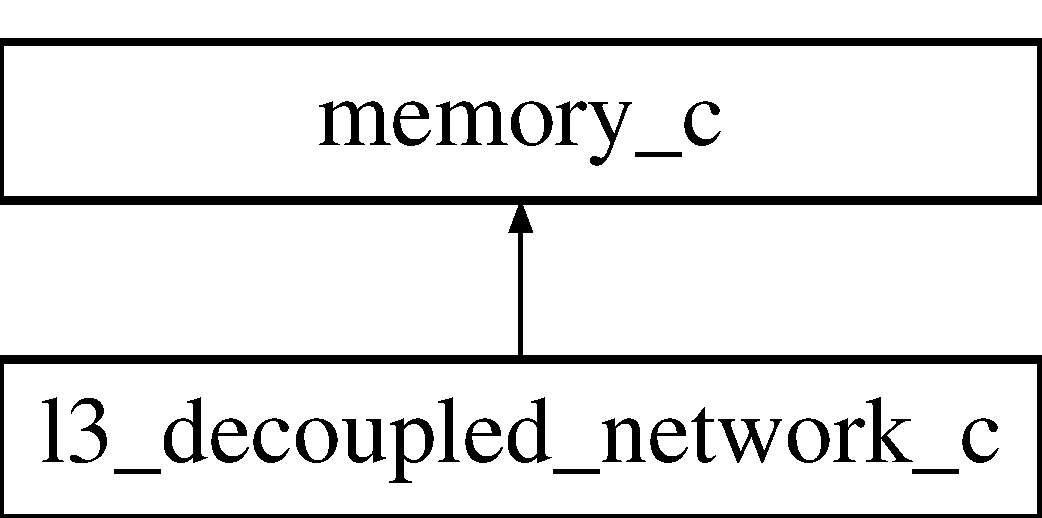
\includegraphics[height=2.000000cm]{classl3__decoupled__network__c}
\end{center}
\end{figure}
\subsection*{Public Member Functions}
\begin{DoxyCompactItemize}
\item 
\hyperlink{classl3__decoupled__network__c_ace5198d467bcf99580a9c593426249a1}{l3\_\-decoupled\_\-network\_\-c} (\hyperlink{classmacsim__c}{macsim\_\-c} $\ast$simBase)
\item 
\hyperlink{classl3__decoupled__network__c_a2b4f7f32f1a19c56449fa9cbbae15cbf}{$\sim$l3\_\-decoupled\_\-network\_\-c} ()
\end{DoxyCompactItemize}


\subsection{Detailed Description}
3-\/Level, Decoupled architecture (2D topology) 

\subsection{Constructor \& Destructor Documentation}
\hypertarget{classl3__decoupled__network__c_ace5198d467bcf99580a9c593426249a1}{
\index{l3\_\-decoupled\_\-network\_\-c@{l3\_\-decoupled\_\-network\_\-c}!l3\_\-decoupled\_\-network\_\-c@{l3\_\-decoupled\_\-network\_\-c}}
\index{l3\_\-decoupled\_\-network\_\-c@{l3\_\-decoupled\_\-network\_\-c}!l3_decoupled_network_c@{l3\_\-decoupled\_\-network\_\-c}}
\subsubsection[{l3\_\-decoupled\_\-network\_\-c}]{\setlength{\rightskip}{0pt plus 5cm}l3\_\-decoupled\_\-network\_\-c::l3\_\-decoupled\_\-network\_\-c (
\begin{DoxyParamCaption}
\item[{{\bf macsim\_\-c} $\ast$}]{ simBase}
\end{DoxyParamCaption}
)}}
\label{classl3__decoupled__network__c_ace5198d467bcf99580a9c593426249a1}
Constructor \hypertarget{classl3__decoupled__network__c_a2b4f7f32f1a19c56449fa9cbbae15cbf}{
\index{l3\_\-decoupled\_\-network\_\-c@{l3\_\-decoupled\_\-network\_\-c}!$\sim$l3\_\-decoupled\_\-network\_\-c@{$\sim$l3\_\-decoupled\_\-network\_\-c}}
\index{$\sim$l3\_\-decoupled\_\-network\_\-c@{$\sim$l3\_\-decoupled\_\-network\_\-c}!l3_decoupled_network_c@{l3\_\-decoupled\_\-network\_\-c}}
\subsubsection[{$\sim$l3\_\-decoupled\_\-network\_\-c}]{\setlength{\rightskip}{0pt plus 5cm}l3\_\-decoupled\_\-network\_\-c::$\sim$l3\_\-decoupled\_\-network\_\-c (
\begin{DoxyParamCaption}
{}
\end{DoxyParamCaption}
)}}
\label{classl3__decoupled__network__c_a2b4f7f32f1a19c56449fa9cbbae15cbf}
Destructor 

The documentation for this class was generated from the following files:\begin{DoxyCompactItemize}
\item 
memory.h\item 
memory.cc\end{DoxyCompactItemize}

\hypertarget{classLINE__Stat}{
\section{LINE\_\-Stat Class Reference}
\label{classLINE__Stat}\index{LINE\_\-Stat@{LINE\_\-Stat}}
}


LINE stat.  




{\ttfamily \#include $<$statistics.h$>$}

Inheritance diagram for LINE\_\-Stat:\begin{figure}[H]
\begin{center}
\leavevmode
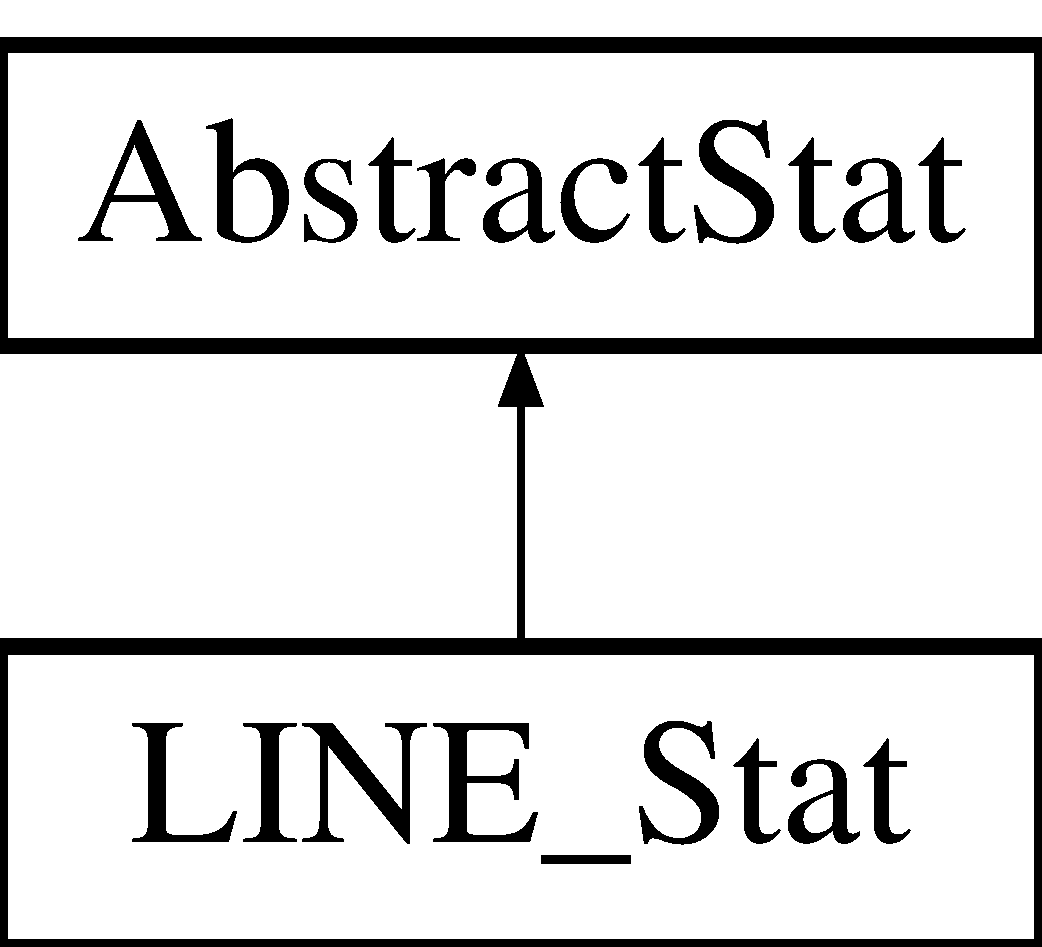
\includegraphics[height=2.000000cm]{classLINE__Stat}
\end{center}
\end{figure}
\subsection*{Public Member Functions}
\begin{DoxyCompactItemize}
\item 
\hyperlink{classLINE__Stat_a47df9b2c458dde5fbd0d626f3160297c}{LINE\_\-Stat} (const string \&str, const string \&outputfilename, long ID)
\item 
virtual \hyperlink{classLINE__Stat_a134f90d180cf462e41595ae257218781}{$\sim$LINE\_\-Stat} ()
\end{DoxyCompactItemize}


\subsection{Detailed Description}
LINE stat. 

\subsection{Constructor \& Destructor Documentation}
\hypertarget{classLINE__Stat_a47df9b2c458dde5fbd0d626f3160297c}{
\index{LINE\_\-Stat@{LINE\_\-Stat}!LINE\_\-Stat@{LINE\_\-Stat}}
\index{LINE\_\-Stat@{LINE\_\-Stat}!LINE_Stat@{LINE\_\-Stat}}
\subsubsection[{LINE\_\-Stat}]{\setlength{\rightskip}{0pt plus 5cm}LINE\_\-Stat::LINE\_\-Stat (
\begin{DoxyParamCaption}
\item[{const string \&}]{ str, }
\item[{const string \&}]{ outputfilename, }
\item[{long}]{ ID}
\end{DoxyParamCaption}
)\hspace{0.3cm}{\ttfamily  \mbox{[}inline\mbox{]}}}}
\label{classLINE__Stat_a47df9b2c458dde5fbd0d626f3160297c}
Constructor. \hypertarget{classLINE__Stat_a134f90d180cf462e41595ae257218781}{
\index{LINE\_\-Stat@{LINE\_\-Stat}!$\sim$LINE\_\-Stat@{$\sim$LINE\_\-Stat}}
\index{$\sim$LINE\_\-Stat@{$\sim$LINE\_\-Stat}!LINE_Stat@{LINE\_\-Stat}}
\subsubsection[{$\sim$LINE\_\-Stat}]{\setlength{\rightskip}{0pt plus 5cm}virtual LINE\_\-Stat::$\sim$LINE\_\-Stat (
\begin{DoxyParamCaption}
{}
\end{DoxyParamCaption}
)\hspace{0.3cm}{\ttfamily  \mbox{[}inline, virtual\mbox{]}}}}
\label{classLINE__Stat_a134f90d180cf462e41595ae257218781}
Destructor. 

The documentation for this class was generated from the following file:\begin{DoxyCompactItemize}
\item 
statistics.h\end{DoxyCompactItemize}

\hypertarget{structltstr__s}{
\section{ltstr\_\-s Struct Reference}
\label{structltstr__s}\index{ltstr\_\-s@{ltstr\_\-s}}
}


provide comparator to \hyperlink{classKnobsContainer}{KnobsContainer} clas  




{\ttfamily \#include $<$knob.h$>$}

\subsection*{Public Member Functions}
\begin{DoxyCompactItemize}
\item 
bool \hyperlink{structltstr__s_a6288346b55245a64173be52f8dcd3ebb}{operator()} (const string \&s1, const string \&s2) const 
\end{DoxyCompactItemize}


\subsection{Detailed Description}
provide comparator to \hyperlink{classKnobsContainer}{KnobsContainer} clas \begin{DoxySeeAlso}{See also}
\hyperlink{classKnobsContainer}{KnobsContainer} 
\end{DoxySeeAlso}


\subsection{Member Function Documentation}
\hypertarget{structltstr__s_a6288346b55245a64173be52f8dcd3ebb}{
\index{ltstr\_\-s@{ltstr\_\-s}!operator()@{operator()}}
\index{operator()@{operator()}!ltstr_s@{ltstr\_\-s}}
\subsubsection[{operator()}]{\setlength{\rightskip}{0pt plus 5cm}bool ltstr\_\-s::operator() (
\begin{DoxyParamCaption}
\item[{const string \&}]{ s1, }
\item[{const string \&}]{ s2}
\end{DoxyParamCaption}
) const\hspace{0.3cm}{\ttfamily  \mbox{[}inline\mbox{]}}}}
\label{structltstr__s_a6288346b55245a64173be52f8dcd3ebb}
operator() -\/ sort comparator 

The documentation for this struct was generated from the following file:\begin{DoxyCompactItemize}
\item 
knob.h\end{DoxyCompactItemize}

\hypertarget{classmacsim__c}{
\section{macsim\_\-c Class Reference}
\label{classmacsim__c}\index{macsim\_\-c@{macsim\_\-c}}
}
\subsection*{Public Member Functions}
\begin{DoxyCompactItemize}
\item 
\hypertarget{classmacsim__c_a7b5f3fe3b4443634b6462a9e07759c84}{
void {\bfseries initialize} (int argc, char $\ast$$\ast$argv)}
\label{classmacsim__c_a7b5f3fe3b4443634b6462a9e07759c84}

\item 
\hypertarget{classmacsim__c_a0ec4f9b71852bdfc3e51348bad0f859b}{
int {\bfseries run\_\-a\_\-cycle} ()}
\label{classmacsim__c_a0ec4f9b71852bdfc3e51348bad0f859b}

\item 
\hypertarget{classmacsim__c_a3466db9d65a3361bd0c92866f6d18391}{
void {\bfseries finalize} ()}
\label{classmacsim__c_a3466db9d65a3361bd0c92866f6d18391}

\item 
\hypertarget{classmacsim__c_a45d3cd10b6ec98efbbb8f0a09495bcbb}{
void {\bfseries init\_\-knobs} (int argc, char $\ast$$\ast$argv)}
\label{classmacsim__c_a45d3cd10b6ec98efbbb8f0a09495bcbb}

\item 
\hypertarget{classmacsim__c_ac92135ddc31916bff6ecb3f53b8d1219}{
void {\bfseries register\_\-functions} (void)}
\label{classmacsim__c_ac92135ddc31916bff6ecb3f53b8d1219}

\item 
\hypertarget{classmacsim__c_a06cf61c8e5a9ab69de0f4f0a49d835b1}{
void {\bfseries init\_\-sim} (void)}
\label{classmacsim__c_a06cf61c8e5a9ab69de0f4f0a49d835b1}

\item 
\hypertarget{classmacsim__c_af66a7ca3a835c9944ea73bcd3df53a78}{
void {\bfseries init\_\-memory} (void)}
\label{classmacsim__c_af66a7ca3a835c9944ea73bcd3df53a78}

\item 
\hypertarget{classmacsim__c_a13f56dcf93b56649f8bfbc9c3f843fb8}{
void {\bfseries init\_\-output\_\-streams} (void)}
\label{classmacsim__c_a13f56dcf93b56649f8bfbc9c3f843fb8}

\item 
\hypertarget{classmacsim__c_aa555d9c437870964d46bdf3ce520a17e}{
void {\bfseries init\_\-cores} (int num\_\-core)}
\label{classmacsim__c_aa555d9c437870964d46bdf3ce520a17e}

\item 
\hypertarget{classmacsim__c_aa51f0db3aa3947724c61f738c26eae79}{
void {\bfseries init\_\-network} (void)}
\label{classmacsim__c_aa51f0db3aa3947724c61f738c26eae79}

\item 
\hypertarget{classmacsim__c_aa6de0832c788be63cf7b6d73c3f0ec34}{
void {\bfseries open\_\-traces} (string trace\_\-file)}
\label{classmacsim__c_aa6de0832c788be63cf7b6d73c3f0ec34}

\item 
\hypertarget{classmacsim__c_a63571fad11e1f3ba698696c5ceddb7f2}{
void {\bfseries deallocate\_\-memory} (void)}
\label{classmacsim__c_a63571fad11e1f3ba698696c5ceddb7f2}

\item 
\hypertarget{classmacsim__c_ac80797445768f61baccbaa02a5221c31}{
void {\bfseries compute\_\-power} (void)}
\label{classmacsim__c_ac80797445768f61baccbaa02a5221c31}

\item 
\hypertarget{classmacsim__c_ab28a994ee52094fb8fae763115704966}{
void {\bfseries fini\_\-sim} (void)}
\label{classmacsim__c_ab28a994ee52094fb8fae763115704966}

\item 
\hypertarget{classmacsim__c_af737aef1a3b6dc3ae2d1f40556258d0d}{
\hyperlink{classrouter__c}{router\_\-c} $\ast$ {\bfseries create\_\-router} ()}
\label{classmacsim__c_af737aef1a3b6dc3ae2d1f40556258d0d}

\item 
\hypertarget{classmacsim__c_a9e5c1c68fac3d4448791ca601c19739a}{
void {\bfseries init\_\-iris\_\-config} (map$<$ string, string $>$ \&params)}
\label{classmacsim__c_a9e5c1c68fac3d4448791ca601c19739a}

\end{DoxyCompactItemize}
\subsection*{Public Attributes}
\begin{DoxyCompactItemize}
\item 
\hypertarget{classmacsim__c_a4baff76941ebb6517b1f7cd6801ad075}{
int {\bfseries m\_\-num\_\-active\_\-threads}}
\label{classmacsim__c_a4baff76941ebb6517b1f7cd6801ad075}

\item 
\hypertarget{classmacsim__c_ad7d692896154e04fe7a9602398d5c5b8}{
int {\bfseries m\_\-num\_\-waiting\_\-dispatched\_\-threads}}
\label{classmacsim__c_ad7d692896154e04fe7a9602398d5c5b8}

\item 
\hypertarget{classmacsim__c_a1bdf950d03675bff1bf62fd6eebd0a51}{
int {\bfseries m\_\-total\_\-num\_\-application}}
\label{classmacsim__c_a1bdf950d03675bff1bf62fd6eebd0a51}

\item 
\hypertarget{classmacsim__c_a77281e97b7c4ca7804f97e37efc15090}{
int {\bfseries m\_\-process\_\-count}}
\label{classmacsim__c_a77281e97b7c4ca7804f97e37efc15090}

\item 
\hypertarget{classmacsim__c_a3229d7207c64d5f65f95c7d0ce117278}{
int {\bfseries m\_\-process\_\-count\_\-without\_\-repeat}}
\label{classmacsim__c_a3229d7207c64d5f65f95c7d0ce117278}

\item 
\hypertarget{classmacsim__c_a8e3d8337db16aa961dcbacbaba75f01d}{
int {\bfseries m\_\-all\_\-threads}}
\label{classmacsim__c_a8e3d8337db16aa961dcbacbaba75f01d}

\item 
\hypertarget{classmacsim__c_a2541778cf745506e34c7106b4b6a2884}{
int {\bfseries m\_\-no\_\-threads\_\-per\_\-block}}
\label{classmacsim__c_a2541778cf745506e34c7106b4b6a2884}

\item 
\hypertarget{classmacsim__c_adb713aaf9e8139239c4c9423b352d6de}{
int {\bfseries m\_\-total\_\-retired\_\-block}}
\label{classmacsim__c_adb713aaf9e8139239c4c9423b352d6de}

\item 
\hypertarget{classmacsim__c_a989dbbce57e8c6e00a7526cf7f22573c}{
int {\bfseries m\_\-num\_\-running\_\-core}}
\label{classmacsim__c_a989dbbce57e8c6e00a7526cf7f22573c}

\item 
\hypertarget{classmacsim__c_ae99ff07858f66a3b8bdaad27cba84ba6}{
bool {\bfseries m\_\-repeat\_\-done}}
\label{classmacsim__c_ae99ff07858f66a3b8bdaad27cba84ba6}

\item 
\hypertarget{classmacsim__c_abbcb39b02a5aa5ce643e36895c6d8c37}{
FILE $\ast$ {\bfseries g\_\-mystdout}}
\label{classmacsim__c_abbcb39b02a5aa5ce643e36895c6d8c37}

\item 
\hypertarget{classmacsim__c_a86a27ed08fa959dd2a7bcbfacf6e00c9}{
FILE $\ast$ {\bfseries g\_\-mystderr}}
\label{classmacsim__c_a86a27ed08fa959dd2a7bcbfacf6e00c9}

\item 
\hypertarget{classmacsim__c_aff0e8865bea89a3c8fe139cdbb1ea8db}{
FILE $\ast$ {\bfseries g\_\-mystatus}}
\label{classmacsim__c_aff0e8865bea89a3c8fe139cdbb1ea8db}

\item 
\hypertarget{classmacsim__c_aa30d75ca4f8ab199477e12ce0e170bb8}{
Counter {\bfseries m\_\-simulation\_\-cycle}}
\label{classmacsim__c_aa30d75ca4f8ab199477e12ce0e170bb8}

\item 
\hypertarget{classmacsim__c_a053cffe61bc44edcf0da911d7a3f685a}{
Counter {\bfseries m\_\-core0\_\-inst\_\-count}}
\label{classmacsim__c_a053cffe61bc44edcf0da911d7a3f685a}

\item 
\hypertarget{classmacsim__c_aa13b8cc432a7611f777e81d06ee46fda}{
Counter {\bfseries m\_\-core\_\-cycle} \mbox{[}MAX\_\-NUM\_\-CORES\mbox{]}}
\label{classmacsim__c_aa13b8cc432a7611f777e81d06ee46fda}

\item 
\hypertarget{classmacsim__c_adfc39eb2e3820c3ae1338bd191c0a7e8}{
int {\bfseries m\_\-end\_\-simulation}}
\label{classmacsim__c_adfc39eb2e3820c3ae1338bd191c0a7e8}

\item 
\hypertarget{classmacsim__c_a721ddb554f496c47e86f68e0ec5bff71}{
\hyperlink{classall__stats__c}{all\_\-stats\_\-c} $\ast$ {\bfseries m\_\-allStats}}
\label{classmacsim__c_a721ddb554f496c47e86f68e0ec5bff71}

\item 
\hypertarget{classmacsim__c_adae560b3d39021be0e86876a73c2c314}{
\hyperlink{classProcessorStatistics}{ProcessorStatistics} $\ast$ {\bfseries m\_\-ProcessorStats}}
\label{classmacsim__c_adae560b3d39021be0e86876a73c2c314}

\item 
\hypertarget{classmacsim__c_a2f33380a1304c84257d50332ca180ae1}{
\hyperlink{classCoreStatistics}{CoreStatistics} $\ast$ {\bfseries m\_\-coreStatsTemplate}}
\label{classmacsim__c_a2f33380a1304c84257d50332ca180ae1}

\item 
\hypertarget{classmacsim__c_ae74712c35d2662c6627da38f2fc96992}{
map$<$ string, ofstream $\ast$ $>$ {\bfseries m\_\-AllStatsOutputStreams}}
\label{classmacsim__c_ae74712c35d2662c6627da38f2fc96992}

\item 
\hypertarget{classmacsim__c_ad59ecc14512d18d335d2bc9c74b3b172}{
ofstream $\ast$ {\bfseries m\_\-core\_\-stat\_\-files} \mbox{[}MAX\_\-NUM\_\-CORES\mbox{]}}
\label{classmacsim__c_ad59ecc14512d18d335d2bc9c74b3b172}

\item 
\hypertarget{classmacsim__c_a8f8662a1f009f001de4473dc99e0b773}{
\hyperlink{classKnobsContainer}{KnobsContainer} $\ast$ {\bfseries m\_\-knobsContainer}}
\label{classmacsim__c_a8f8662a1f009f001de4473dc99e0b773}

\item 
\hypertarget{classmacsim__c_aa24b0c838a197877aa3aa726fbc23d3d}{
\hyperlink{classall__knobs__c}{all\_\-knobs\_\-c} $\ast$ {\bfseries m\_\-knobs}}
\label{classmacsim__c_aa24b0c838a197877aa3aa726fbc23d3d}

\item 
\hypertarget{classmacsim__c_a560adba247bfd673eb14421abc9ac241}{
bool {\bfseries m\_\-core\_\-end\_\-trace} \mbox{[}MAX\_\-NUM\_\-CORES\mbox{]}}
\label{classmacsim__c_a560adba247bfd673eb14421abc9ac241}

\item 
\hypertarget{classmacsim__c_aaf2644cd3bd0b14d2329dca9b79bf4b6}{
bool {\bfseries m\_\-sim\_\-end} \mbox{[}MAX\_\-NUM\_\-CORES\mbox{]}}
\label{classmacsim__c_aaf2644cd3bd0b14d2329dca9b79bf4b6}

\item 
\hypertarget{classmacsim__c_ab940fac1230e2f823573771ef30e204b}{
bool {\bfseries m\_\-core\_\-started} \mbox{[}MAX\_\-NUM\_\-CORES\mbox{]}}
\label{classmacsim__c_ab940fac1230e2f823573771ef30e204b}

\item 
\hypertarget{classmacsim__c_af8a5d5ad197669d975ab385491bd2bff}{
\hyperlink{classcore__c}{core\_\-c} $\ast$ {\bfseries m\_\-core\_\-pointers} \mbox{[}MAX\_\-NUM\_\-CORES\mbox{]}}
\label{classmacsim__c_af8a5d5ad197669d975ab385491bd2bff}

\item 
\hypertarget{classmacsim__c_ab07b52a087b78401fc29cf15f504e192}{
\hyperlink{classmemory__c}{memory\_\-c} $\ast$ {\bfseries m\_\-memory}}
\label{classmacsim__c_ab07b52a087b78401fc29cf15f504e192}

\item 
\hypertarget{classmacsim__c_a9e630e22667f3c213e3a7bf324774273}{
\hyperlink{classnoc__c}{noc\_\-c} $\ast$ {\bfseries m\_\-noc}}
\label{classmacsim__c_a9e630e22667f3c213e3a7bf324774273}

\item 
\hypertarget{classmacsim__c_afe8210473b0073f7ad72cee863fc98be}{
queue$<$ int $>$ {\bfseries m\_\-x86\_\-core\_\-pool}}
\label{classmacsim__c_afe8210473b0073f7ad72cee863fc98be}

\item 
\hypertarget{classmacsim__c_ae9ead2bf6d0a161f72a50a5c22562752}{
queue$<$ int $>$ {\bfseries m\_\-ptx\_\-core\_\-pool}}
\label{classmacsim__c_ae9ead2bf6d0a161f72a50a5c22562752}

\item 
\hypertarget{classmacsim__c_ac694c08a40e42f83ef383bbe9266fb30}{
\hyperlink{classbug__detector__c}{bug\_\-detector\_\-c} $\ast$ {\bfseries m\_\-bug\_\-detector}}
\label{classmacsim__c_ac694c08a40e42f83ef383bbe9266fb30}

\item 
\hypertarget{classmacsim__c_a5f048e64e73788988fc8874226c0645d}{
\hyperlink{classmulti__key__map__c}{multi\_\-key\_\-map\_\-c} $\ast$ {\bfseries m\_\-block\_\-id\_\-mapper}}
\label{classmacsim__c_a5f048e64e73788988fc8874226c0645d}

\item 
\hypertarget{classmacsim__c_ad038c08ff8163e6a93aaea780aef4ed1}{
\hyperlink{classprocess__manager__c}{process\_\-manager\_\-c} $\ast$ {\bfseries m\_\-process\_\-manager}}
\label{classmacsim__c_ad038c08ff8163e6a93aaea780aef4ed1}

\item 
\hypertarget{classmacsim__c_a46d8f1f11c59a31e69299792fc2a118f}{
\hyperlink{classuop__c}{uop\_\-c} $\ast$ {\bfseries m\_\-invalid\_\-uop}}
\label{classmacsim__c_a46d8f1f11c59a31e69299792fc2a118f}

\item 
\hypertarget{classmacsim__c_ad6d9b4e9baa7d966f63233cfa7ebc38f}{
\hyperlink{classei__power__c}{ei\_\-power\_\-c} $\ast$ {\bfseries m\_\-ei\_\-power}}
\label{classmacsim__c_ad6d9b4e9baa7d966f63233cfa7ebc38f}

\item 
\hypertarget{classmacsim__c_a88df74852e044fcf67a5d696b48bc666}{
\hyperlink{classpool__c}{pool\_\-c}$<$ \hyperlink{structthread__s}{thread\_\-s} $>$ $\ast$ {\bfseries m\_\-thread\_\-pool}}
\label{classmacsim__c_a88df74852e044fcf67a5d696b48bc666}

\item 
\hypertarget{classmacsim__c_ae6961ebdcddb7f04c6f30c26206855af}{
\hyperlink{classpool__c}{pool\_\-c}$<$ \hyperlink{structsection__info__s}{section\_\-info\_\-s} $>$ $\ast$ {\bfseries m\_\-section\_\-pool}}
\label{classmacsim__c_ae6961ebdcddb7f04c6f30c26206855af}

\item 
\hypertarget{classmacsim__c_afda2ca57edf97e12c107dcea3d4c02cb}{
\hyperlink{classpool__c}{pool\_\-c}$<$ \hyperlink{classmem__map__entry__c}{mem\_\-map\_\-entry\_\-c} $>$ $\ast$ {\bfseries m\_\-mem\_\-map\_\-entry\_\-pool}}
\label{classmacsim__c_afda2ca57edf97e12c107dcea3d4c02cb}

\item 
\hypertarget{classmacsim__c_a65d74f24dbb74178906f184663282390}{
\hyperlink{classpool__c}{pool\_\-c}$<$ \hyperlink{classheartbeat__s}{heartbeat\_\-s} $>$ $\ast$ {\bfseries m\_\-heartbeat\_\-pool}}
\label{classmacsim__c_a65d74f24dbb74178906f184663282390}

\item 
\hypertarget{classmacsim__c_aa6275ca9790f25e3532b066b1a24f3d2}{
\hyperlink{classpool__c}{pool\_\-c}$<$ \hyperlink{classbp__recovery__info__c}{bp\_\-recovery\_\-info\_\-c} $>$ $\ast$ {\bfseries m\_\-bp\_\-recovery\_\-info\_\-pool}}
\label{classmacsim__c_aa6275ca9790f25e3532b066b1a24f3d2}

\item 
\hypertarget{classmacsim__c_ab5544e875d5e35378fa6496ede6459c7}{
\hyperlink{classpool__c}{pool\_\-c}$<$ \hyperlink{structthread__trace__info__node__s}{thread\_\-trace\_\-info\_\-node\_\-s} $>$ $\ast$ {\bfseries m\_\-trace\_\-node\_\-pool}}
\label{classmacsim__c_ab5544e875d5e35378fa6496ede6459c7}

\item 
\hypertarget{classmacsim__c_a781123061f8045a8d85f744bd0ccd07c}{
\hyperlink{classpool__c}{pool\_\-c}$<$ \hyperlink{classuop__c}{uop\_\-c} $>$ $\ast$ {\bfseries m\_\-uop\_\-pool}}
\label{classmacsim__c_a781123061f8045a8d85f744bd0ccd07c}

\item 
\hypertarget{classmacsim__c_afe2d09324626df7fb2d3fe8d8e04b404}{
unordered\_\-map$<$ int, \hyperlink{classhash__c}{hash\_\-c}$<$ \hyperlink{classinst__info__s}{inst\_\-info\_\-s} $>$ $\ast$ $>$ {\bfseries m\_\-inst\_\-info\_\-hash}}
\label{classmacsim__c_afe2d09324626df7fb2d3fe8d8e04b404}

\item 
\hypertarget{classmacsim__c_a097596db621a77dc4b8854e7ba13d944}{
unordered\_\-map$<$ int, \hyperlink{structblock__schedule__info__s}{block\_\-schedule\_\-info\_\-s} $\ast$ $>$ {\bfseries m\_\-block\_\-schedule\_\-info}}
\label{classmacsim__c_a097596db621a77dc4b8854e7ba13d944}

\item 
\hypertarget{classmacsim__c_a04c5be42aae87b1b4dc8398b40c4bebc}{
unordered\_\-map$<$ int, \hyperlink{structprocess__s}{process\_\-s} $\ast$ $>$ {\bfseries m\_\-sim\_\-processes}}
\label{classmacsim__c_a04c5be42aae87b1b4dc8398b40c4bebc}

\item 
\hypertarget{classmacsim__c_a82e823eac7f1edaef124ae20edb8b905}{
unordered\_\-map$<$ int, \hyperlink{structthread__stat__s}{thread\_\-stat\_\-s} $\ast$ $>$ {\bfseries m\_\-thread\_\-stats}}
\label{classmacsim__c_a82e823eac7f1edaef124ae20edb8b905}

\item 
\hypertarget{classmacsim__c_ad66c0fae20f8da217136c93789aa552d}{
struct timeval {\bfseries m\_\-begin\_\-sim}}
\label{classmacsim__c_ad66c0fae20f8da217136c93789aa552d}

\item 
\hypertarget{classmacsim__c_ad150572cf94097d5bb0e302e7ee36735}{
struct timeval {\bfseries m\_\-end\_\-sim}}
\label{classmacsim__c_ad150572cf94097d5bb0e302e7ee36735}

\item 
\hypertarget{classmacsim__c_a717e3a5b0427dfbb69a8fa545f2a02be}{
\hyperlink{classtrace__read__c}{trace\_\-read\_\-c} $\ast$ {\bfseries m\_\-trace\_\-reader}}
\label{classmacsim__c_a717e3a5b0427dfbb69a8fa545f2a02be}

\item 
\hypertarget{classmacsim__c_a49d3f59d80273b9706879c58a6019a4b}{
\hyperlink{classrouter__wrapper__c}{router\_\-wrapper\_\-c} $\ast$ {\bfseries m\_\-router}}
\label{classmacsim__c_a49d3f59d80273b9706879c58a6019a4b}

\item 
\hypertarget{classmacsim__c_a8ea8fcd8da294b674cdfa2b894052698}{
map$<$ string, string $>$ {\bfseries m\_\-iris\_\-params}}
\label{classmacsim__c_a8ea8fcd8da294b674cdfa2b894052698}

\item 
\hypertarget{classmacsim__c_a0fe5a937f6d33cc093ff4c65b837061c}{
Topology $\ast$ {\bfseries m\_\-iris\_\-network}}
\label{classmacsim__c_a0fe5a937f6d33cc093ff4c65b837061c}

\item 
\hypertarget{classmacsim__c_a37bad1fa5d96c92c437f4be6d4d343e6}{
Topology $\ast$ {\bfseries tp}}
\label{classmacsim__c_a37bad1fa5d96c92c437f4be6d4d343e6}

\item 
\hypertarget{classmacsim__c_acdb35ca43741de0d9a8f9602500ca8f7}{
uint {\bfseries no\_\-nodes}}
\label{classmacsim__c_acdb35ca43741de0d9a8f9602500ca8f7}

\item 
\hypertarget{classmacsim__c_a5cb68870036c6d0b2a3f7f3e10f1b54d}{
int {\bfseries Mytid}}
\label{classmacsim__c_a5cb68870036c6d0b2a3f7f3e10f1b54d}

\item 
\hypertarget{classmacsim__c_a2868eea271765027b03ac37d75750721}{
FILE $\ast$ {\bfseries log\_\-file}}
\label{classmacsim__c_a2868eea271765027b03ac37d75750721}

\item 
\hypertarget{classmacsim__c_ac60101dda5b72c0e35ddcd6e8a791ddc}{
string {\bfseries network\_\-filename}}
\label{classmacsim__c_ac60101dda5b72c0e35ddcd6e8a791ddc}

\item 
\hypertarget{classmacsim__c_adf5e19f936f69235ab7cb034b6b084db}{
vector$<$ ManifoldProcessor $\ast$ $>$ {\bfseries m\_\-macsim\_\-terminals}}
\label{classmacsim__c_adf5e19f936f69235ab7cb034b6b084db}

\item 
\hypertarget{classmacsim__c_ae89f4011df241d6aebd32fe9a96f54f1}{
\hyperlink{classcache__partition__framework__c}{cache\_\-partition\_\-framework\_\-c} $\ast$ {\bfseries m\_\-PCL}}
\label{classmacsim__c_ae89f4011df241d6aebd32fe9a96f54f1}

\item 
\hypertarget{classmacsim__c_a8fd5541cc2e4c85af747d546df7dc7bd}{
manifold::kernel::Clock $\ast$ {\bfseries master\_\-clock}}
\label{classmacsim__c_a8fd5541cc2e4c85af747d546df7dc7bd}

\item 
\hypertarget{classmacsim__c_a7617bbe4e19a06e3182deb4e3d930621}{
double {\bfseries avg\_\-power}}
\label{classmacsim__c_a7617bbe4e19a06e3182deb4e3d930621}

\item 
\hypertarget{classmacsim__c_a37d6e196da37d9f4f80e5d7a3e7c0604}{
double {\bfseries total\_\-energy}}
\label{classmacsim__c_a37d6e196da37d9f4f80e5d7a3e7c0604}

\item 
\hypertarget{classmacsim__c_aa1da137da2034ad320493d8a495b2336}{
int {\bfseries total\_\-packets}}
\label{classmacsim__c_aa1da137da2034ad320493d8a495b2336}

\end{DoxyCompactItemize}
\subsection*{Private Attributes}
\begin{DoxyCompactItemize}
\item 
\hypertarget{classmacsim__c_a9a5c822e0f844e6f712630fef243abf0}{
\hyperlink{classmacsim__c}{macsim\_\-c} $\ast$ {\bfseries m\_\-simBase}}
\label{classmacsim__c_a9a5c822e0f844e6f712630fef243abf0}

\end{DoxyCompactItemize}


The documentation for this class was generated from the following files:\begin{DoxyCompactItemize}
\item 
macsim.h\item 
macsim.cc\end{DoxyCompactItemize}

\hypertarget{classmap__c}{
\section{map\_\-c Class Reference}
\label{classmap__c}\index{map\_\-c@{map\_\-c}}
}


register dependence mapping  




{\ttfamily \#include $<$map.h$>$}

\subsection*{Public Member Functions}
\begin{DoxyCompactItemize}
\item 
\hyperlink{classmap__c_a5da8b3e64f7caac52a295a7e9b933f75}{map\_\-c} (\hyperlink{classmacsim__c}{macsim\_\-c} $\ast$simBase)
\item 
\hyperlink{classmap__c_a0ea194b2e9f7b55924fb542d78d8ca6f}{$\sim$map\_\-c} ()
\item 
void \hyperlink{classmap__c_a15ec904cf369a18d9b96954852783575}{set\_\-not\_\-rdy\_\-bit} (\hyperlink{classuop__c}{uop\_\-c} $\ast$uop, uns bit)
\item 
void \hyperlink{classmap__c_adbabb202c0a3811b5075b857f821f029}{add\_\-src\_\-from\_\-map\_\-entry} (\hyperlink{classuop__c}{uop\_\-c} $\ast$uop, uns src\_\-num, \hyperlink{classmap__entry__c}{map\_\-entry\_\-c} $\ast$map\_\-entry, Dep\_\-Type type)
\item 
void \hyperlink{classmap__c_aae742289893034f94a5618efde509f84}{add\_\-src\_\-from\_\-uop} (\hyperlink{classuop__c}{uop\_\-c} $\ast$uop, \hyperlink{classuop__c}{uop\_\-c} $\ast$src\_\-uop, Dep\_\-Type type)
\item 
void \hyperlink{classmap__c_a823103c7d95ab23d6b115bcb787768e7}{map\_\-mem\_\-dep} (\hyperlink{classuop__c}{uop\_\-c} $\ast$uop)
\item 
void \hyperlink{classmap__c_ab8b07395663470c39f25ed31fe93fd68}{update\_\-map} (\hyperlink{classuop__c}{uop\_\-c} $\ast$uop)
\item 
void \hyperlink{classmap__c_a7369eb469d7d7a3e88cd25e73db7d101}{map\_\-uop} (\hyperlink{classuop__c}{uop\_\-c} $\ast$uop)
\item 
void \hyperlink{classmap__c_ad1e67ca582adc46312128a69301b59f3}{read\_\-reg\_\-map} (\hyperlink{classuop__c}{uop\_\-c} $\ast$uop)
\item 
void \hyperlink{classmap__c_a007d7ff6b649658cb5b83e4abc87fd7f}{read\_\-store\_\-map} (\hyperlink{classuop__c}{uop\_\-c} $\ast$uop)
\item 
void \hyperlink{classmap__c_a705da8acf7e3d36776e12e83b3dab0f6}{update\_\-store\_\-hash} (\hyperlink{classuop__c}{uop\_\-c} $\ast$uop)
\item 
\hyperlink{classuop__c}{uop\_\-c} $\ast$ \hyperlink{classmap__c_a313f6a7f163ae4b749274d66a0b570a6}{add\_\-store\_\-deps} (\hyperlink{classuop__c}{uop\_\-c} $\ast$uop)
\item 
void \hyperlink{classmap__c_a44553352d9550ac88fb9159be1f6c8c6}{delete\_\-store\_\-hash\_\-entry} (\hyperlink{classuop__c}{uop\_\-c} $\ast$uop)
\item 
void \hyperlink{classmap__c_ac64891f7ad08cd54f76f7069df0df816}{delete\_\-map} (int)
\end{DoxyCompactItemize}
\subsection*{Public Attributes}
\begin{DoxyCompactItemize}
\item 
\hyperlink{classhash__c}{hash\_\-c}$<$ \hyperlink{classmap__data__c}{map\_\-data\_\-c} $>$ $\ast$ \hyperlink{classmap__c_af14fbb514a865af51d89f827d72d17f3}{m\_\-core\_\-map\_\-data}
\end{DoxyCompactItemize}
\subsection*{Private Attributes}
\begin{DoxyCompactItemize}
\item 
\hyperlink{classmacsim__c}{macsim\_\-c} $\ast$ \hyperlink{classmap__c_ad004224b761c096deeeaca078b2ba22d}{m\_\-simBase}
\end{DoxyCompactItemize}


\subsection{Detailed Description}
register dependence mapping 

\subsection{Constructor \& Destructor Documentation}
\hypertarget{classmap__c_a5da8b3e64f7caac52a295a7e9b933f75}{
\index{map\_\-c@{map\_\-c}!map\_\-c@{map\_\-c}}
\index{map\_\-c@{map\_\-c}!map_c@{map\_\-c}}
\subsubsection[{map\_\-c}]{\setlength{\rightskip}{0pt plus 5cm}map\_\-c::map\_\-c (
\begin{DoxyParamCaption}
\item[{{\bf macsim\_\-c} $\ast$}]{ simBase}
\end{DoxyParamCaption}
)}}
\label{classmap__c_a5da8b3e64f7caac52a295a7e9b933f75}
Constructor 
\begin{DoxyParams}{Parameters}
\item[{\em simBase}]-\/ Pointer to base simulation class for perf/stat counters \end{DoxyParams}
\hypertarget{classmap__c_a0ea194b2e9f7b55924fb542d78d8ca6f}{
\index{map\_\-c@{map\_\-c}!$\sim$map\_\-c@{$\sim$map\_\-c}}
\index{$\sim$map\_\-c@{$\sim$map\_\-c}!map_c@{map\_\-c}}
\subsubsection[{$\sim$map\_\-c}]{\setlength{\rightskip}{0pt plus 5cm}map\_\-c::$\sim$map\_\-c (
\begin{DoxyParamCaption}
{}
\end{DoxyParamCaption}
)}}
\label{classmap__c_a0ea194b2e9f7b55924fb542d78d8ca6f}
Destructor 

\subsection{Member Function Documentation}
\hypertarget{classmap__c_adbabb202c0a3811b5075b857f821f029}{
\index{map\_\-c@{map\_\-c}!add\_\-src\_\-from\_\-map\_\-entry@{add\_\-src\_\-from\_\-map\_\-entry}}
\index{add\_\-src\_\-from\_\-map\_\-entry@{add\_\-src\_\-from\_\-map\_\-entry}!map_c@{map\_\-c}}
\subsubsection[{add\_\-src\_\-from\_\-map\_\-entry}]{\setlength{\rightskip}{0pt plus 5cm}void map\_\-c::add\_\-src\_\-from\_\-map\_\-entry (
\begin{DoxyParamCaption}
\item[{{\bf uop\_\-c} $\ast$}]{ uop, }
\item[{uns}]{ src\_\-num, }
\item[{{\bf map\_\-entry\_\-c} $\ast$}]{ map\_\-entry, }
\item[{Dep\_\-Type}]{ type}
\end{DoxyParamCaption}
)}}
\label{classmap__c_adbabb202c0a3811b5075b857f821f029}
Set dependent-\/source information. An uop will check each source's dependence. 
\begin{DoxyParams}{Parameters}
\item[{\em uop}]myself \item[{\em src\_\-num}]source id (register \#) of the uop \item[{\em map\_\-entry}]map entry corresponding to the register \# \item[{\em type}]register dependence (always) \end{DoxyParams}
\hypertarget{classmap__c_aae742289893034f94a5618efde509f84}{
\index{map\_\-c@{map\_\-c}!add\_\-src\_\-from\_\-uop@{add\_\-src\_\-from\_\-uop}}
\index{add\_\-src\_\-from\_\-uop@{add\_\-src\_\-from\_\-uop}!map_c@{map\_\-c}}
\subsubsection[{add\_\-src\_\-from\_\-uop}]{\setlength{\rightskip}{0pt plus 5cm}void map\_\-c::add\_\-src\_\-from\_\-uop (
\begin{DoxyParamCaption}
\item[{{\bf uop\_\-c} $\ast$}]{ uop, }
\item[{{\bf uop\_\-c} $\ast$}]{ src\_\-uop, }
\item[{Dep\_\-Type}]{ type}
\end{DoxyParamCaption}
)}}
\label{classmap__c_aae742289893034f94a5618efde509f84}
Set dependent-\/source information from a source uop \hypertarget{classmap__c_a313f6a7f163ae4b749274d66a0b570a6}{
\index{map\_\-c@{map\_\-c}!add\_\-store\_\-deps@{add\_\-store\_\-deps}}
\index{add\_\-store\_\-deps@{add\_\-store\_\-deps}!map_c@{map\_\-c}}
\subsubsection[{add\_\-store\_\-deps}]{\setlength{\rightskip}{0pt plus 5cm}{\bf uop\_\-c} $\ast$ map\_\-c::add\_\-store\_\-deps (
\begin{DoxyParamCaption}
\item[{{\bf uop\_\-c} $\ast$}]{ uop}
\end{DoxyParamCaption}
)}}
\label{classmap__c_a313f6a7f163ae4b749274d66a0b570a6}
Add load-\/store dependence \hypertarget{classmap__c_ac64891f7ad08cd54f76f7069df0df816}{
\index{map\_\-c@{map\_\-c}!delete\_\-map@{delete\_\-map}}
\index{delete\_\-map@{delete\_\-map}!map_c@{map\_\-c}}
\subsubsection[{delete\_\-map}]{\setlength{\rightskip}{0pt plus 5cm}void map\_\-c::delete\_\-map (
\begin{DoxyParamCaption}
\item[{int}]{ tid}
\end{DoxyParamCaption}
)}}
\label{classmap__c_ac64891f7ad08cd54f76f7069df0df816}
When a thread has been terminated, delete entire dependence information \hypertarget{classmap__c_a44553352d9550ac88fb9159be1f6c8c6}{
\index{map\_\-c@{map\_\-c}!delete\_\-store\_\-hash\_\-entry@{delete\_\-store\_\-hash\_\-entry}}
\index{delete\_\-store\_\-hash\_\-entry@{delete\_\-store\_\-hash\_\-entry}!map_c@{map\_\-c}}
\subsubsection[{delete\_\-store\_\-hash\_\-entry}]{\setlength{\rightskip}{0pt plus 5cm}void map\_\-c::delete\_\-store\_\-hash\_\-entry (
\begin{DoxyParamCaption}
\item[{{\bf uop\_\-c} $\ast$}]{ uop}
\end{DoxyParamCaption}
)}}
\label{classmap__c_a44553352d9550ac88fb9159be1f6c8c6}
Delete a store dependence information when store instruction has been retired. \hypertarget{classmap__c_a823103c7d95ab23d6b115bcb787768e7}{
\index{map\_\-c@{map\_\-c}!map\_\-mem\_\-dep@{map\_\-mem\_\-dep}}
\index{map\_\-mem\_\-dep@{map\_\-mem\_\-dep}!map_c@{map\_\-c}}
\subsubsection[{map\_\-mem\_\-dep}]{\setlength{\rightskip}{0pt plus 5cm}void map\_\-c::map\_\-mem\_\-dep (
\begin{DoxyParamCaption}
\item[{{\bf uop\_\-c} $\ast$}]{ uop}
\end{DoxyParamCaption}
)}}
\label{classmap__c_a823103c7d95ab23d6b115bcb787768e7}
Add memory dependence information \hypertarget{classmap__c_a7369eb469d7d7a3e88cd25e73db7d101}{
\index{map\_\-c@{map\_\-c}!map\_\-uop@{map\_\-uop}}
\index{map\_\-uop@{map\_\-uop}!map_c@{map\_\-c}}
\subsubsection[{map\_\-uop}]{\setlength{\rightskip}{0pt plus 5cm}void map\_\-c::map\_\-uop (
\begin{DoxyParamCaption}
\item[{{\bf uop\_\-c} $\ast$}]{ uop}
\end{DoxyParamCaption}
)}}
\label{classmap__c_a7369eb469d7d7a3e88cd25e73db7d101}
Wrapper function to add register/memory dependences. \begin{DoxySeeAlso}{See also}
\hyperlink{classfrontend__c_a5de715a12e87c609121b884ebc880a27}{frontend\_\-c::process\_\-ifetch} 
\end{DoxySeeAlso}
\hypertarget{classmap__c_ad1e67ca582adc46312128a69301b59f3}{
\index{map\_\-c@{map\_\-c}!read\_\-reg\_\-map@{read\_\-reg\_\-map}}
\index{read\_\-reg\_\-map@{read\_\-reg\_\-map}!map_c@{map\_\-c}}
\subsubsection[{read\_\-reg\_\-map}]{\setlength{\rightskip}{0pt plus 5cm}void map\_\-c::read\_\-reg\_\-map (
\begin{DoxyParamCaption}
\item[{{\bf uop\_\-c} $\ast$}]{ uop}
\end{DoxyParamCaption}
)}}
\label{classmap__c_ad1e67ca582adc46312128a69301b59f3}
Read register dependence map. New register dependences will be added for each source registers \hypertarget{classmap__c_a007d7ff6b649658cb5b83e4abc87fd7f}{
\index{map\_\-c@{map\_\-c}!read\_\-store\_\-map@{read\_\-store\_\-map}}
\index{read\_\-store\_\-map@{read\_\-store\_\-map}!map_c@{map\_\-c}}
\subsubsection[{read\_\-store\_\-map}]{\setlength{\rightskip}{0pt plus 5cm}void map\_\-c::read\_\-store\_\-map (
\begin{DoxyParamCaption}
\item[{{\bf uop\_\-c} $\ast$}]{ uop}
\end{DoxyParamCaption}
)}}
\label{classmap__c_a007d7ff6b649658cb5b83e4abc87fd7f}
Read store dependence map. When a memory operation calls this function, new store dependence information will be added. \hypertarget{classmap__c_a15ec904cf369a18d9b96954852783575}{
\index{map\_\-c@{map\_\-c}!set\_\-not\_\-rdy\_\-bit@{set\_\-not\_\-rdy\_\-bit}}
\index{set\_\-not\_\-rdy\_\-bit@{set\_\-not\_\-rdy\_\-bit}!map_c@{map\_\-c}}
\subsubsection[{set\_\-not\_\-rdy\_\-bit}]{\setlength{\rightskip}{0pt plus 5cm}void map\_\-c::set\_\-not\_\-rdy\_\-bit (
\begin{DoxyParamCaption}
\item[{{\bf uop\_\-c} $\ast$}]{ uop, }
\item[{uns}]{ bit}
\end{DoxyParamCaption}
)}}
\label{classmap__c_a15ec904cf369a18d9b96954852783575}
Set source N not ready \hypertarget{classmap__c_ab8b07395663470c39f25ed31fe93fd68}{
\index{map\_\-c@{map\_\-c}!update\_\-map@{update\_\-map}}
\index{update\_\-map@{update\_\-map}!map_c@{map\_\-c}}
\subsubsection[{update\_\-map}]{\setlength{\rightskip}{0pt plus 5cm}void map\_\-c::update\_\-map (
\begin{DoxyParamCaption}
\item[{{\bf uop\_\-c} $\ast$}]{ uop}
\end{DoxyParamCaption}
)}}
\label{classmap__c_ab8b07395663470c39f25ed31fe93fd68}
Update map data with destination id of an uop. By adding destination register in the map, all following dependent uops will be affected. \hypertarget{classmap__c_a705da8acf7e3d36776e12e83b3dab0f6}{
\index{map\_\-c@{map\_\-c}!update\_\-store\_\-hash@{update\_\-store\_\-hash}}
\index{update\_\-store\_\-hash@{update\_\-store\_\-hash}!map_c@{map\_\-c}}
\subsubsection[{update\_\-store\_\-hash}]{\setlength{\rightskip}{0pt plus 5cm}void map\_\-c::update\_\-store\_\-hash (
\begin{DoxyParamCaption}
\item[{{\bf uop\_\-c} $\ast$}]{ uop}
\end{DoxyParamCaption}
)}}
\label{classmap__c_a705da8acf7e3d36776e12e83b3dab0f6}
Update load-\/store dependence 

\subsection{Member Data Documentation}
\hypertarget{classmap__c_af14fbb514a865af51d89f827d72d17f3}{
\index{map\_\-c@{map\_\-c}!m\_\-core\_\-map\_\-data@{m\_\-core\_\-map\_\-data}}
\index{m\_\-core\_\-map\_\-data@{m\_\-core\_\-map\_\-data}!map_c@{map\_\-c}}
\subsubsection[{m\_\-core\_\-map\_\-data}]{\setlength{\rightskip}{0pt plus 5cm}{\bf hash\_\-c}$<${\bf map\_\-data\_\-c}$>$$\ast$ {\bf map\_\-c::m\_\-core\_\-map\_\-data}}}
\label{classmap__c_af14fbb514a865af51d89f827d72d17f3}
per thread dependence table \hypertarget{classmap__c_ad004224b761c096deeeaca078b2ba22d}{
\index{map\_\-c@{map\_\-c}!m\_\-simBase@{m\_\-simBase}}
\index{m\_\-simBase@{m\_\-simBase}!map_c@{map\_\-c}}
\subsubsection[{m\_\-simBase}]{\setlength{\rightskip}{0pt plus 5cm}{\bf macsim\_\-c}$\ast$ {\bf map\_\-c::m\_\-simBase}\hspace{0.3cm}{\ttfamily  \mbox{[}private\mbox{]}}}}
\label{classmap__c_ad004224b761c096deeeaca078b2ba22d}
\hyperlink{classmacsim__c}{macsim\_\-c} base class for simulation globals 

The documentation for this class was generated from the following files:\begin{DoxyCompactItemize}
\item 
map.h\item 
map.cc\end{DoxyCompactItemize}

\hypertarget{classmap__data__c}{
\section{map\_\-data\_\-c Class Reference}
\label{classmap__data__c}\index{map\_\-data\_\-c@{map\_\-data\_\-c}}
}


data structure holding dependence information  




{\ttfamily \#include $<$map.h$>$}

\subsection*{Public Member Functions}
\begin{DoxyCompactItemize}
\item 
\hyperlink{classmap__data__c_a207c7c5d293a92fa6ff9d7c8bd342171}{map\_\-data\_\-c} (\hyperlink{classmacsim__c}{macsim\_\-c} $\ast$simBase)
\item 
void \hyperlink{classmap__data__c_a6432fa4d113cfa96f91a8b8489013490}{initialize} ()
\end{DoxyCompactItemize}
\subsection*{Public Attributes}
\begin{DoxyCompactItemize}
\item 
\hyperlink{classmap__entry__c}{map\_\-entry\_\-c} \hyperlink{classmap__data__c_a6d513b4921be0e1da6ca2360e799453a}{m\_\-reg\_\-map} \mbox{[}NUM\_\-REG\_\-IDS $\ast$2\mbox{]}
\item 
bool \hyperlink{classmap__data__c_a8ff9086064a196500af89171acf094f4}{m\_\-map\_\-flags} \mbox{[}NUM\_\-REG\_\-IDS $\ast$2\mbox{]}
\item 
\hyperlink{classmap__entry__c}{map\_\-entry\_\-c} \hyperlink{classmap__data__c_a0fdc6d2ec6990c2dcf5851280020453f}{m\_\-last\_\-store} \mbox{[}2\mbox{]}
\item 
bool \hyperlink{classmap__data__c_a43198f297f11ac7c3626469abedc194f}{m\_\-last\_\-store\_\-flag}
\item 
\hyperlink{classhash__c}{hash\_\-c}$<$ \hyperlink{classmem__map__entry__c}{mem\_\-map\_\-entry\_\-c} $>$ $\ast$ \hyperlink{classmap__data__c_a48ae320988c5045e28f10321feae64f8}{m\_\-oracle\_\-mem\_\-hash}
\end{DoxyCompactItemize}
\subsection*{Private Attributes}
\begin{DoxyCompactItemize}
\item 
\hyperlink{classmacsim__c}{macsim\_\-c} $\ast$ \hyperlink{classmap__data__c_ac4f6915212a9d8a7df898996070a18a3}{m\_\-simBase}
\end{DoxyCompactItemize}


\subsection{Detailed Description}
data structure holding dependence information 

\subsection{Constructor \& Destructor Documentation}
\hypertarget{classmap__data__c_a207c7c5d293a92fa6ff9d7c8bd342171}{
\index{map\_\-data\_\-c@{map\_\-data\_\-c}!map\_\-data\_\-c@{map\_\-data\_\-c}}
\index{map\_\-data\_\-c@{map\_\-data\_\-c}!map_data_c@{map\_\-data\_\-c}}
\subsubsection[{map\_\-data\_\-c}]{\setlength{\rightskip}{0pt plus 5cm}map\_\-data\_\-c::map\_\-data\_\-c (
\begin{DoxyParamCaption}
\item[{{\bf macsim\_\-c} $\ast$}]{ simBase}
\end{DoxyParamCaption}
)}}
\label{classmap__data__c_a207c7c5d293a92fa6ff9d7c8bd342171}
Constructor 

\subsection{Member Function Documentation}
\hypertarget{classmap__data__c_a6432fa4d113cfa96f91a8b8489013490}{
\index{map\_\-data\_\-c@{map\_\-data\_\-c}!initialize@{initialize}}
\index{initialize@{initialize}!map_data_c@{map\_\-data\_\-c}}
\subsubsection[{initialize}]{\setlength{\rightskip}{0pt plus 5cm}void map\_\-data\_\-c::initialize (
\begin{DoxyParamCaption}
{}
\end{DoxyParamCaption}
)}}
\label{classmap__data__c_a6432fa4d113cfa96f91a8b8489013490}
Initialization 

\subsection{Member Data Documentation}
\hypertarget{classmap__data__c_a0fdc6d2ec6990c2dcf5851280020453f}{
\index{map\_\-data\_\-c@{map\_\-data\_\-c}!m\_\-last\_\-store@{m\_\-last\_\-store}}
\index{m\_\-last\_\-store@{m\_\-last\_\-store}!map_data_c@{map\_\-data\_\-c}}
\subsubsection[{m\_\-last\_\-store}]{\setlength{\rightskip}{0pt plus 5cm}{\bf map\_\-entry\_\-c} {\bf map\_\-data\_\-c::m\_\-last\_\-store}\mbox{[}2\mbox{]}}}
\label{classmap__data__c_a0fdc6d2ec6990c2dcf5851280020453f}
last store map entry \hypertarget{classmap__data__c_a43198f297f11ac7c3626469abedc194f}{
\index{map\_\-data\_\-c@{map\_\-data\_\-c}!m\_\-last\_\-store\_\-flag@{m\_\-last\_\-store\_\-flag}}
\index{m\_\-last\_\-store\_\-flag@{m\_\-last\_\-store\_\-flag}!map_data_c@{map\_\-data\_\-c}}
\subsubsection[{m\_\-last\_\-store\_\-flag}]{\setlength{\rightskip}{0pt plus 5cm}bool {\bf map\_\-data\_\-c::m\_\-last\_\-store\_\-flag}}}
\label{classmap__data__c_a43198f297f11ac7c3626469abedc194f}
last store flag \hypertarget{classmap__data__c_a8ff9086064a196500af89171acf094f4}{
\index{map\_\-data\_\-c@{map\_\-data\_\-c}!m\_\-map\_\-flags@{m\_\-map\_\-flags}}
\index{m\_\-map\_\-flags@{m\_\-map\_\-flags}!map_data_c@{map\_\-data\_\-c}}
\subsubsection[{m\_\-map\_\-flags}]{\setlength{\rightskip}{0pt plus 5cm}bool {\bf map\_\-data\_\-c::m\_\-map\_\-flags}\mbox{[}NUM\_\-REG\_\-IDS $\ast$2\mbox{]}}}
\label{classmap__data__c_a8ff9086064a196500af89171acf094f4}
map data exist for the source \hypertarget{classmap__data__c_a48ae320988c5045e28f10321feae64f8}{
\index{map\_\-data\_\-c@{map\_\-data\_\-c}!m\_\-oracle\_\-mem\_\-hash@{m\_\-oracle\_\-mem\_\-hash}}
\index{m\_\-oracle\_\-mem\_\-hash@{m\_\-oracle\_\-mem\_\-hash}!map_data_c@{map\_\-data\_\-c}}
\subsubsection[{m\_\-oracle\_\-mem\_\-hash}]{\setlength{\rightskip}{0pt plus 5cm}{\bf hash\_\-c}$<${\bf mem\_\-map\_\-entry\_\-c}$>$$\ast$ {\bf map\_\-data\_\-c::m\_\-oracle\_\-mem\_\-hash}}}
\label{classmap__data__c_a48ae320988c5045e28f10321feae64f8}
oracle memory hash \hypertarget{classmap__data__c_a6d513b4921be0e1da6ca2360e799453a}{
\index{map\_\-data\_\-c@{map\_\-data\_\-c}!m\_\-reg\_\-map@{m\_\-reg\_\-map}}
\index{m\_\-reg\_\-map@{m\_\-reg\_\-map}!map_data_c@{map\_\-data\_\-c}}
\subsubsection[{m\_\-reg\_\-map}]{\setlength{\rightskip}{0pt plus 5cm}{\bf map\_\-entry\_\-c} {\bf map\_\-data\_\-c::m\_\-reg\_\-map}\mbox{[}NUM\_\-REG\_\-IDS $\ast$2\mbox{]}}}
\label{classmap__data__c_a6d513b4921be0e1da6ca2360e799453a}
register map per source \hypertarget{classmap__data__c_ac4f6915212a9d8a7df898996070a18a3}{
\index{map\_\-data\_\-c@{map\_\-data\_\-c}!m\_\-simBase@{m\_\-simBase}}
\index{m\_\-simBase@{m\_\-simBase}!map_data_c@{map\_\-data\_\-c}}
\subsubsection[{m\_\-simBase}]{\setlength{\rightskip}{0pt plus 5cm}{\bf macsim\_\-c}$\ast$ {\bf map\_\-data\_\-c::m\_\-simBase}\hspace{0.3cm}{\ttfamily  \mbox{[}private\mbox{]}}}}
\label{classmap__data__c_ac4f6915212a9d8a7df898996070a18a3}
\hyperlink{classmacsim__c}{macsim\_\-c} base class for simulation globals 

The documentation for this class was generated from the following files:\begin{DoxyCompactItemize}
\item 
map.h\item 
map.cc\end{DoxyCompactItemize}

\hypertarget{classmap__entry__c}{
\section{map\_\-entry\_\-c Class Reference}
\label{classmap__entry__c}\index{map\_\-entry\_\-c@{map\_\-entry\_\-c}}
}


dependence information  




{\ttfamily \#include $<$map.h$>$}

\subsection*{Public Attributes}
\begin{DoxyCompactItemize}
\item 
\hyperlink{classuop__c}{uop\_\-c} $\ast$ \hyperlink{classmap__entry__c_ab6464a295f3c4c34ab222df2cd521b48}{m\_\-uop}
\item 
Counter \hyperlink{classmap__entry__c_a8652b806200144aa94a38f420aee08d2}{m\_\-uop\_\-num}
\item 
Counter \hyperlink{classmap__entry__c_ad89c46be260e96eac067256a202c9b5e}{m\_\-inst\_\-num}
\item 
Addr \hyperlink{classmap__entry__c_a9950a129015b7524a2623549f58aefcc}{m\_\-pc}
\item 
Counter \hyperlink{classmap__entry__c_a0a8a7d10cd323dd0df59c45f4af1e464}{m\_\-unique\_\-num}
\item 
int \hyperlink{classmap__entry__c_a3d60eba98c1ca2e9e41dc99ab84ae686}{m\_\-thread\_\-id}
\item 
int \hyperlink{classmap__entry__c_ac290f8ec57135c8a9570f9963cb0256c}{m\_\-mem\_\-type}
\end{DoxyCompactItemize}


\subsection{Detailed Description}
dependence information 

\subsection{Member Data Documentation}
\hypertarget{classmap__entry__c_ad89c46be260e96eac067256a202c9b5e}{
\index{map\_\-entry\_\-c@{map\_\-entry\_\-c}!m\_\-inst\_\-num@{m\_\-inst\_\-num}}
\index{m\_\-inst\_\-num@{m\_\-inst\_\-num}!map_entry_c@{map\_\-entry\_\-c}}
\subsubsection[{m\_\-inst\_\-num}]{\setlength{\rightskip}{0pt plus 5cm}Counter {\bf map\_\-entry\_\-c::m\_\-inst\_\-num}}}
\label{classmap__entry__c_ad89c46be260e96eac067256a202c9b5e}
uop's instruction number \hypertarget{classmap__entry__c_ac290f8ec57135c8a9570f9963cb0256c}{
\index{map\_\-entry\_\-c@{map\_\-entry\_\-c}!m\_\-mem\_\-type@{m\_\-mem\_\-type}}
\index{m\_\-mem\_\-type@{m\_\-mem\_\-type}!map_entry_c@{map\_\-entry\_\-c}}
\subsubsection[{m\_\-mem\_\-type}]{\setlength{\rightskip}{0pt plus 5cm}int {\bf map\_\-entry\_\-c::m\_\-mem\_\-type}}}
\label{classmap__entry__c_ac290f8ec57135c8a9570f9963cb0256c}
memory type \hypertarget{classmap__entry__c_a9950a129015b7524a2623549f58aefcc}{
\index{map\_\-entry\_\-c@{map\_\-entry\_\-c}!m\_\-pc@{m\_\-pc}}
\index{m\_\-pc@{m\_\-pc}!map_entry_c@{map\_\-entry\_\-c}}
\subsubsection[{m\_\-pc}]{\setlength{\rightskip}{0pt plus 5cm}Addr {\bf map\_\-entry\_\-c::m\_\-pc}}}
\label{classmap__entry__c_a9950a129015b7524a2623549f58aefcc}
pc address \hypertarget{classmap__entry__c_a3d60eba98c1ca2e9e41dc99ab84ae686}{
\index{map\_\-entry\_\-c@{map\_\-entry\_\-c}!m\_\-thread\_\-id@{m\_\-thread\_\-id}}
\index{m\_\-thread\_\-id@{m\_\-thread\_\-id}!map_entry_c@{map\_\-entry\_\-c}}
\subsubsection[{m\_\-thread\_\-id}]{\setlength{\rightskip}{0pt plus 5cm}int {\bf map\_\-entry\_\-c::m\_\-thread\_\-id}}}
\label{classmap__entry__c_a3d60eba98c1ca2e9e41dc99ab84ae686}
thread id \hypertarget{classmap__entry__c_a0a8a7d10cd323dd0df59c45f4af1e464}{
\index{map\_\-entry\_\-c@{map\_\-entry\_\-c}!m\_\-unique\_\-num@{m\_\-unique\_\-num}}
\index{m\_\-unique\_\-num@{m\_\-unique\_\-num}!map_entry_c@{map\_\-entry\_\-c}}
\subsubsection[{m\_\-unique\_\-num}]{\setlength{\rightskip}{0pt plus 5cm}Counter {\bf map\_\-entry\_\-c::m\_\-unique\_\-num}}}
\label{classmap__entry__c_a0a8a7d10cd323dd0df59c45f4af1e464}
uop's unique number \hypertarget{classmap__entry__c_ab6464a295f3c4c34ab222df2cd521b48}{
\index{map\_\-entry\_\-c@{map\_\-entry\_\-c}!m\_\-uop@{m\_\-uop}}
\index{m\_\-uop@{m\_\-uop}!map_entry_c@{map\_\-entry\_\-c}}
\subsubsection[{m\_\-uop}]{\setlength{\rightskip}{0pt plus 5cm}{\bf uop\_\-c}$\ast$ {\bf map\_\-entry\_\-c::m\_\-uop}}}
\label{classmap__entry__c_ab6464a295f3c4c34ab222df2cd521b48}
uop pointer \hypertarget{classmap__entry__c_a8652b806200144aa94a38f420aee08d2}{
\index{map\_\-entry\_\-c@{map\_\-entry\_\-c}!m\_\-uop\_\-num@{m\_\-uop\_\-num}}
\index{m\_\-uop\_\-num@{m\_\-uop\_\-num}!map_entry_c@{map\_\-entry\_\-c}}
\subsubsection[{m\_\-uop\_\-num}]{\setlength{\rightskip}{0pt plus 5cm}Counter {\bf map\_\-entry\_\-c::m\_\-uop\_\-num}}}
\label{classmap__entry__c_a8652b806200144aa94a38f420aee08d2}
uop number 

The documentation for this class was generated from the following file:\begin{DoxyCompactItemize}
\item 
map.h\end{DoxyCompactItemize}

\hypertarget{classmem__map__entry__c}{
\section{mem\_\-map\_\-entry\_\-c Class Reference}
\label{classmem__map__entry__c}\index{mem\_\-map\_\-entry\_\-c@{mem\_\-map\_\-entry\_\-c}}
}


data structure holding memory dependence information  




{\ttfamily \#include $<$map.h$>$}

\subsection*{Public Attributes}
\begin{DoxyCompactItemize}
\item 
\hyperlink{classuop__c}{uop\_\-c} $\ast$ \hyperlink{classmem__map__entry__c_a3ca3d13eb2521e21ed2776293f4f20c4}{m\_\-uop} \mbox{[}BYTES\_\-IN\_\-QUADWORD\mbox{]}
\item 
Quad \hyperlink{classmem__map__entry__c_a3d7080bd5290849a0ee2482d38a66cf1}{m\_\-data}
\item 
uns8 \hyperlink{classmem__map__entry__c_aa4d50f7f30287bd33107a8579f898be5}{m\_\-store\_\-mask}
\end{DoxyCompactItemize}


\subsection{Detailed Description}
data structure holding memory dependence information 

\subsection{Member Data Documentation}
\hypertarget{classmem__map__entry__c_a3d7080bd5290849a0ee2482d38a66cf1}{
\index{mem\_\-map\_\-entry\_\-c@{mem\_\-map\_\-entry\_\-c}!m\_\-data@{m\_\-data}}
\index{m\_\-data@{m\_\-data}!mem_map_entry_c@{mem\_\-map\_\-entry\_\-c}}
\subsubsection[{m\_\-data}]{\setlength{\rightskip}{0pt plus 5cm}Quad {\bf mem\_\-map\_\-entry\_\-c::m\_\-data}}}
\label{classmem__map__entry__c_a3d7080bd5290849a0ee2482d38a66cf1}
memory dependence data \hypertarget{classmem__map__entry__c_aa4d50f7f30287bd33107a8579f898be5}{
\index{mem\_\-map\_\-entry\_\-c@{mem\_\-map\_\-entry\_\-c}!m\_\-store\_\-mask@{m\_\-store\_\-mask}}
\index{m\_\-store\_\-mask@{m\_\-store\_\-mask}!mem_map_entry_c@{mem\_\-map\_\-entry\_\-c}}
\subsubsection[{m\_\-store\_\-mask}]{\setlength{\rightskip}{0pt plus 5cm}uns8 {\bf mem\_\-map\_\-entry\_\-c::m\_\-store\_\-mask}}}
\label{classmem__map__entry__c_aa4d50f7f30287bd33107a8579f898be5}
shows position of all distinct stores supplying a partial value to this map entry \hypertarget{classmem__map__entry__c_a3ca3d13eb2521e21ed2776293f4f20c4}{
\index{mem\_\-map\_\-entry\_\-c@{mem\_\-map\_\-entry\_\-c}!m\_\-uop@{m\_\-uop}}
\index{m\_\-uop@{m\_\-uop}!mem_map_entry_c@{mem\_\-map\_\-entry\_\-c}}
\subsubsection[{m\_\-uop}]{\setlength{\rightskip}{0pt plus 5cm}{\bf uop\_\-c}$\ast$ {\bf mem\_\-map\_\-entry\_\-c::m\_\-uop}\mbox{[}BYTES\_\-IN\_\-QUADWORD\mbox{]}}}
\label{classmem__map__entry__c_a3ca3d13eb2521e21ed2776293f4f20c4}
last op to write (invalid when committed) 

The documentation for this class was generated from the following file:\begin{DoxyCompactItemize}
\item 
map.h\end{DoxyCompactItemize}

\hypertarget{classmem__req__c}{
\section{mem\_\-req\_\-c Class Reference}
\label{classmem__req__c}\index{mem\_\-req\_\-c@{mem\_\-req\_\-c}}
}
\subsection*{Static Public Attributes}
\begin{DoxyCompactItemize}
\item 
static const char $\ast$ {\bfseries mem\_\-req\_\-type\_\-name} \mbox{[}MAX\_\-MEM\_\-REQ\_\-TYPE\mbox{]}
\item 
static const char $\ast$ {\bfseries mem\_\-state} \mbox{[}MEM\_\-STATE\_\-MAX\mbox{]}
\end{DoxyCompactItemize}


\subsection{Member Data Documentation}
\hypertarget{classmem__req__c_a3f50969bb3742eb9b01e5390c99589ab}{
\index{mem\_\-req\_\-c@{mem\_\-req\_\-c}!mem\_\-req\_\-type\_\-name@{mem\_\-req\_\-type\_\-name}}
\index{mem\_\-req\_\-type\_\-name@{mem\_\-req\_\-type\_\-name}!mem_req_c@{mem\_\-req\_\-c}}
\subsubsection[{mem\_\-req\_\-type\_\-name}]{\setlength{\rightskip}{0pt plus 5cm}const char $\ast$ mem\_\-req\_\-c::mem\_\-req\_\-type\_\-name\hspace{0.3cm}{\ttfamily  \mbox{[}static\mbox{]}}}}
\label{classmem__req__c_a3f50969bb3742eb9b01e5390c99589ab}
{\bfseries Initial value:}
\begin{DoxyCode}
 {
  "IFETCH",
  "DFETCH",
  "DSTORE",
  "IPRF",
  "DPRF",
  "WB",
  "SW_DPRF",
  "SW_DPRF_NTA",
  "SW_DPRF_T0",
  "SW_DPRF_T1",
  "SW_DPRF_T2",
}
\end{DoxyCode}
\hypertarget{classmem__req__c_aa1a55583f778ef7c4f29047a8ff8553b}{
\index{mem\_\-req\_\-c@{mem\_\-req\_\-c}!mem\_\-state@{mem\_\-state}}
\index{mem\_\-state@{mem\_\-state}!mem_req_c@{mem\_\-req\_\-c}}
\subsubsection[{mem\_\-state}]{\setlength{\rightskip}{0pt plus 5cm}const char $\ast$ mem\_\-req\_\-c::mem\_\-state\hspace{0.3cm}{\ttfamily  \mbox{[}static\mbox{]}}}}
\label{classmem__req__c_aa1a55583f778ef7c4f29047a8ff8553b}
{\bfseries Initial value:}
\begin{DoxyCode}
 {
  "MEM_INV",
  "MEM_NEW",
  "MEM_MERGED",
  "MEM_OUTQUEUE_NEW",
  "MEM_IN_NOC",
  "MEM_OUT_FILL",
  "MEM_OUT_WB",
  "MEM_FILL_NEW",
  "MEM_FILL_WAIT_DONE",
  "MEM_FILL_WAIT_FILL",
  "MEM_DRAM_START",
  "MEM_DRAM_CMD",
  "MEM_DRAM_DATA",
  "MEM_DRAM_DONE",
  "MEM_NOC_START",
  "MEM_NOC_DONE",
}
\end{DoxyCode}


The documentation for this class was generated from the following files:\begin{DoxyCompactItemize}
\item 
memreq\_\-info.h\item 
memreq\_\-info.cc\end{DoxyCompactItemize}

\hypertarget{structmem__req__s}{
\section{mem\_\-req\_\-s Struct Reference}
\label{structmem__req__s}\index{mem\_\-req\_\-s@{mem\_\-req\_\-s}}
}


memory request data structure  




{\ttfamily \#include $<$memreq\_\-info.h$>$}

\subsection*{Public Member Functions}
\begin{DoxyCompactItemize}
\item 
\hyperlink{structmem__req__s_a8adcd0b63a42bd45874514db51e5500d}{mem\_\-req\_\-s} (\hyperlink{classmacsim__c}{macsim\_\-c} $\ast$simBase)
\end{DoxyCompactItemize}
\subsection*{Public Attributes}
\begin{DoxyCompactItemize}
\item 
int \hyperlink{structmem__req__s_aa1ce2eda1984474c5304bc52e0f96445}{m\_\-id}
\item 
int \hyperlink{structmem__req__s_a256acada11160343b8fd7b0f410c80c8}{m\_\-appl\_\-id}
\item 
int \hyperlink{structmem__req__s_ae79108aead8de2855cccdaf981cb81f8}{m\_\-core\_\-id}
\item 
int \hyperlink{structmem__req__s_a8f90cf134af2d0965d436574f77693ef}{m\_\-thread\_\-id}
\item 
int \hyperlink{structmem__req__s_ad160765e9454b1e36dc188805585a3ff}{m\_\-block\_\-id}
\item 
Mem\_\-Req\_\-State \hyperlink{structmem__req__s_a06db9581649b020ba9b693397a2b90f7}{m\_\-state}
\item 
Mem\_\-Req\_\-Type \hyperlink{structmem__req__s_a9cc3c968ca7bea8f7e9585b2aaea0ede}{m\_\-type}
\item 
Counter \hyperlink{structmem__req__s_af7a1252bce4c150639539ba1551a3d33}{m\_\-priority}
\item 
Addr \hyperlink{structmem__req__s_a835153e595f8931c1259d7074c6f1019}{m\_\-addr}
\item 
uns \hyperlink{structmem__req__s_a4d0488370174c8f3b7200cc4658c9d32}{m\_\-size}
\item 
Counter \hyperlink{structmem__req__s_a61a80fc35da503e4334d0dc79e2c3ff5}{m\_\-rdy\_\-cycle}
\item 
Addr \hyperlink{structmem__req__s_a94e91af0e42f5b41778fed51aa5614c7}{m\_\-pc}
\item 
uns8 \hyperlink{structmem__req__s_a230c4f2a949162d7417337f4a06ac14c}{m\_\-prefetcher\_\-id}
\item 
Addr \hyperlink{structmem__req__s_aa33fc982a960ecccb76d44fc0d3ac039}{m\_\-pref\_\-loadPC}
\item 
bool \hyperlink{structmem__req__s_a5f13d6f19dd50e8cc25ef9a795842007}{m\_\-ptx}
\item 
\hyperlink{classqueue__c}{queue\_\-c} $\ast$ \hyperlink{structmem__req__s_a01bfbc2d9326cadcb66c356740d10eb9}{m\_\-queue}
\item 
int \hyperlink{structmem__req__s_a136b8b016a5e922dbc766490e5478b3e}{m\_\-cache\_\-id} \mbox{[}MEM\_\-LAST\mbox{]}
\item 
\hyperlink{classuop__c}{uop\_\-c} $\ast$ \hyperlink{structmem__req__s_ac912d0ec02a27cbd6d126ab1482c201b}{m\_\-uop}
\item 
Counter \hyperlink{structmem__req__s_a2755c0f5390e5101c68dcfa17835f060}{m\_\-in}
\item 
bool \hyperlink{structmem__req__s_ad03ad960252da07338a40f46a4c2f0da}{m\_\-dirty}
\item 
bool \hyperlink{structmem__req__s_af3191e32583b52626b60ed9817a3768a}{m\_\-done}
\item 
\hyperlink{structmem__req__s}{mem\_\-req\_\-s} $\ast$ \hyperlink{structmem__req__s_a3b87d3a717d7bb0f87634a8c7504a5b5}{m\_\-merged\_\-req}
\item 
int \hyperlink{structmem__req__s_ad9e7fb008600b23a34448c1cb8efe835}{m\_\-msg\_\-type}
\item 
int \hyperlink{structmem__req__s_a858166c5e9fa9c8078088c6e04941a9f}{m\_\-msg\_\-src}
\item 
int \hyperlink{structmem__req__s_a16204d197e4dab80807c947af110160e}{m\_\-msg\_\-dst}
\item 
int \hyperlink{structmem__req__s_a45680e38670bb6ed3b65f11dc22e4c4a}{m\_\-bypass}
\item 
\hypertarget{structmem__req__s_a4c3cf0a762ff754afd5d5170a106de09}{
bool {\bfseries m\_\-skip}}
\label{structmem__req__s_a4c3cf0a762ff754afd5d5170a106de09}

\item 
\hypertarget{structmem__req__s_ad1e86b986bd6153a898b0581bbcf1efb}{
Counter {\bfseries m\_\-noc\_\-cycle}}
\label{structmem__req__s_ad1e86b986bd6153a898b0581bbcf1efb}

\item 
\hyperlink{classmacsim__c}{macsim\_\-c} $\ast$ \hyperlink{structmem__req__s_a7477749204e08ce0a7aa41607a23d74f}{m\_\-simBase}
\item 
function$<$ bool(\hyperlink{structmem__req__s}{mem\_\-req\_\-s} $\ast$) \hyperlink{structmem__req__s_a3170f1143be13457e12b0d0c6f8beb25}{m\_\-done\_\-func} )
\item 
list$<$ \hyperlink{structmem__req__s}{mem\_\-req\_\-s} $\ast$ $>$ \hyperlink{structmem__req__s_a821fa41554b58f5c5b1b751b6e5f1721}{m\_\-merge}
\end{DoxyCompactItemize}


\subsection{Detailed Description}
memory request data structure 

\subsection{Constructor \& Destructor Documentation}
\hypertarget{structmem__req__s_a8adcd0b63a42bd45874514db51e5500d}{
\index{mem\_\-req\_\-s@{mem\_\-req\_\-s}!mem\_\-req\_\-s@{mem\_\-req\_\-s}}
\index{mem\_\-req\_\-s@{mem\_\-req\_\-s}!mem_req_s@{mem\_\-req\_\-s}}
\subsubsection[{mem\_\-req\_\-s}]{\setlength{\rightskip}{0pt plus 5cm}mem\_\-req\_\-s::mem\_\-req\_\-s (
\begin{DoxyParamCaption}
\item[{{\bf macsim\_\-c} $\ast$}]{ simBase}
\end{DoxyParamCaption}
)}}
\label{structmem__req__s_a8adcd0b63a42bd45874514db51e5500d}
Constructor 

\subsection{Member Data Documentation}
\hypertarget{structmem__req__s_a835153e595f8931c1259d7074c6f1019}{
\index{mem\_\-req\_\-s@{mem\_\-req\_\-s}!m\_\-addr@{m\_\-addr}}
\index{m\_\-addr@{m\_\-addr}!mem_req_s@{mem\_\-req\_\-s}}
\subsubsection[{m\_\-addr}]{\setlength{\rightskip}{0pt plus 5cm}Addr {\bf mem\_\-req\_\-s::m\_\-addr}}}
\label{structmem__req__s_a835153e595f8931c1259d7074c6f1019}
request address \hypertarget{structmem__req__s_a256acada11160343b8fd7b0f410c80c8}{
\index{mem\_\-req\_\-s@{mem\_\-req\_\-s}!m\_\-appl\_\-id@{m\_\-appl\_\-id}}
\index{m\_\-appl\_\-id@{m\_\-appl\_\-id}!mem_req_s@{mem\_\-req\_\-s}}
\subsubsection[{m\_\-appl\_\-id}]{\setlength{\rightskip}{0pt plus 5cm}int {\bf mem\_\-req\_\-s::m\_\-appl\_\-id}}}
\label{structmem__req__s_a256acada11160343b8fd7b0f410c80c8}
application id \hypertarget{structmem__req__s_ad160765e9454b1e36dc188805585a3ff}{
\index{mem\_\-req\_\-s@{mem\_\-req\_\-s}!m\_\-block\_\-id@{m\_\-block\_\-id}}
\index{m\_\-block\_\-id@{m\_\-block\_\-id}!mem_req_s@{mem\_\-req\_\-s}}
\subsubsection[{m\_\-block\_\-id}]{\setlength{\rightskip}{0pt plus 5cm}int {\bf mem\_\-req\_\-s::m\_\-block\_\-id}}}
\label{structmem__req__s_ad160765e9454b1e36dc188805585a3ff}
GPU block id \hypertarget{structmem__req__s_a45680e38670bb6ed3b65f11dc22e4c4a}{
\index{mem\_\-req\_\-s@{mem\_\-req\_\-s}!m\_\-bypass@{m\_\-bypass}}
\index{m\_\-bypass@{m\_\-bypass}!mem_req_s@{mem\_\-req\_\-s}}
\subsubsection[{m\_\-bypass}]{\setlength{\rightskip}{0pt plus 5cm}int {\bf mem\_\-req\_\-s::m\_\-bypass}}}
\label{structmem__req__s_a45680e38670bb6ed3b65f11dc22e4c4a}
bypass last level cache \hypertarget{structmem__req__s_a136b8b016a5e922dbc766490e5478b3e}{
\index{mem\_\-req\_\-s@{mem\_\-req\_\-s}!m\_\-cache\_\-id@{m\_\-cache\_\-id}}
\index{m\_\-cache\_\-id@{m\_\-cache\_\-id}!mem_req_s@{mem\_\-req\_\-s}}
\subsubsection[{m\_\-cache\_\-id}]{\setlength{\rightskip}{0pt plus 5cm}int {\bf mem\_\-req\_\-s::m\_\-cache\_\-id}\mbox{[}MEM\_\-LAST\mbox{]}}}
\label{structmem__req__s_a136b8b016a5e922dbc766490e5478b3e}
each level cache id \hypertarget{structmem__req__s_ae79108aead8de2855cccdaf981cb81f8}{
\index{mem\_\-req\_\-s@{mem\_\-req\_\-s}!m\_\-core\_\-id@{m\_\-core\_\-id}}
\index{m\_\-core\_\-id@{m\_\-core\_\-id}!mem_req_s@{mem\_\-req\_\-s}}
\subsubsection[{m\_\-core\_\-id}]{\setlength{\rightskip}{0pt plus 5cm}int {\bf mem\_\-req\_\-s::m\_\-core\_\-id}}}
\label{structmem__req__s_ae79108aead8de2855cccdaf981cb81f8}
core id \hypertarget{structmem__req__s_ad03ad960252da07338a40f46a4c2f0da}{
\index{mem\_\-req\_\-s@{mem\_\-req\_\-s}!m\_\-dirty@{m\_\-dirty}}
\index{m\_\-dirty@{m\_\-dirty}!mem_req_s@{mem\_\-req\_\-s}}
\subsubsection[{m\_\-dirty}]{\setlength{\rightskip}{0pt plus 5cm}bool {\bf mem\_\-req\_\-s::m\_\-dirty}}}
\label{structmem__req__s_ad03ad960252da07338a40f46a4c2f0da}
wb request? \hypertarget{structmem__req__s_af3191e32583b52626b60ed9817a3768a}{
\index{mem\_\-req\_\-s@{mem\_\-req\_\-s}!m\_\-done@{m\_\-done}}
\index{m\_\-done@{m\_\-done}!mem_req_s@{mem\_\-req\_\-s}}
\subsubsection[{m\_\-done}]{\setlength{\rightskip}{0pt plus 5cm}bool {\bf mem\_\-req\_\-s::m\_\-done}}}
\label{structmem__req__s_af3191e32583b52626b60ed9817a3768a}
request done flag \hypertarget{structmem__req__s_a3170f1143be13457e12b0d0c6f8beb25}{
\index{mem\_\-req\_\-s@{mem\_\-req\_\-s}!m\_\-done\_\-func@{m\_\-done\_\-func}}
\index{m\_\-done\_\-func@{m\_\-done\_\-func}!mem_req_s@{mem\_\-req\_\-s}}
\subsubsection[{m\_\-done\_\-func}]{\setlength{\rightskip}{0pt plus 5cm}function$<$bool ({\bf mem\_\-req\_\-s}$\ast$) {\bf mem\_\-req\_\-s::m\_\-done\_\-func})}}
\label{structmem__req__s_a3170f1143be13457e12b0d0c6f8beb25}
done function \hypertarget{structmem__req__s_aa1ce2eda1984474c5304bc52e0f96445}{
\index{mem\_\-req\_\-s@{mem\_\-req\_\-s}!m\_\-id@{m\_\-id}}
\index{m\_\-id@{m\_\-id}!mem_req_s@{mem\_\-req\_\-s}}
\subsubsection[{m\_\-id}]{\setlength{\rightskip}{0pt plus 5cm}int {\bf mem\_\-req\_\-s::m\_\-id}}}
\label{structmem__req__s_aa1ce2eda1984474c5304bc52e0f96445}
unique request id \hypertarget{structmem__req__s_a2755c0f5390e5101c68dcfa17835f060}{
\index{mem\_\-req\_\-s@{mem\_\-req\_\-s}!m\_\-in@{m\_\-in}}
\index{m\_\-in@{m\_\-in}!mem_req_s@{mem\_\-req\_\-s}}
\subsubsection[{m\_\-in}]{\setlength{\rightskip}{0pt plus 5cm}Counter {\bf mem\_\-req\_\-s::m\_\-in}}}
\label{structmem__req__s_a2755c0f5390e5101c68dcfa17835f060}
request inserted cycle \hypertarget{structmem__req__s_a821fa41554b58f5c5b1b751b6e5f1721}{
\index{mem\_\-req\_\-s@{mem\_\-req\_\-s}!m\_\-merge@{m\_\-merge}}
\index{m\_\-merge@{m\_\-merge}!mem_req_s@{mem\_\-req\_\-s}}
\subsubsection[{m\_\-merge}]{\setlength{\rightskip}{0pt plus 5cm}list$<${\bf mem\_\-req\_\-s}$\ast$$>$ {\bf mem\_\-req\_\-s::m\_\-merge}}}
\label{structmem__req__s_a821fa41554b58f5c5b1b751b6e5f1721}
merged request list \hypertarget{structmem__req__s_a3b87d3a717d7bb0f87634a8c7504a5b5}{
\index{mem\_\-req\_\-s@{mem\_\-req\_\-s}!m\_\-merged\_\-req@{m\_\-merged\_\-req}}
\index{m\_\-merged\_\-req@{m\_\-merged\_\-req}!mem_req_s@{mem\_\-req\_\-s}}
\subsubsection[{m\_\-merged\_\-req}]{\setlength{\rightskip}{0pt plus 5cm}{\bf mem\_\-req\_\-s}$\ast$ {\bf mem\_\-req\_\-s::m\_\-merged\_\-req}}}
\label{structmem__req__s_a3b87d3a717d7bb0f87634a8c7504a5b5}
merged request \hypertarget{structmem__req__s_a16204d197e4dab80807c947af110160e}{
\index{mem\_\-req\_\-s@{mem\_\-req\_\-s}!m\_\-msg\_\-dst@{m\_\-msg\_\-dst}}
\index{m\_\-msg\_\-dst@{m\_\-msg\_\-dst}!mem_req_s@{mem\_\-req\_\-s}}
\subsubsection[{m\_\-msg\_\-dst}]{\setlength{\rightskip}{0pt plus 5cm}int {\bf mem\_\-req\_\-s::m\_\-msg\_\-dst}}}
\label{structmem__req__s_a16204d197e4dab80807c947af110160e}
destination node id \hypertarget{structmem__req__s_a858166c5e9fa9c8078088c6e04941a9f}{
\index{mem\_\-req\_\-s@{mem\_\-req\_\-s}!m\_\-msg\_\-src@{m\_\-msg\_\-src}}
\index{m\_\-msg\_\-src@{m\_\-msg\_\-src}!mem_req_s@{mem\_\-req\_\-s}}
\subsubsection[{m\_\-msg\_\-src}]{\setlength{\rightskip}{0pt plus 5cm}int {\bf mem\_\-req\_\-s::m\_\-msg\_\-src}}}
\label{structmem__req__s_a858166c5e9fa9c8078088c6e04941a9f}
source node id \hypertarget{structmem__req__s_ad9e7fb008600b23a34448c1cb8efe835}{
\index{mem\_\-req\_\-s@{mem\_\-req\_\-s}!m\_\-msg\_\-type@{m\_\-msg\_\-type}}
\index{m\_\-msg\_\-type@{m\_\-msg\_\-type}!mem_req_s@{mem\_\-req\_\-s}}
\subsubsection[{m\_\-msg\_\-type}]{\setlength{\rightskip}{0pt plus 5cm}int {\bf mem\_\-req\_\-s::m\_\-msg\_\-type}}}
\label{structmem__req__s_ad9e7fb008600b23a34448c1cb8efe835}
noc request type \hypertarget{structmem__req__s_a94e91af0e42f5b41778fed51aa5614c7}{
\index{mem\_\-req\_\-s@{mem\_\-req\_\-s}!m\_\-pc@{m\_\-pc}}
\index{m\_\-pc@{m\_\-pc}!mem_req_s@{mem\_\-req\_\-s}}
\subsubsection[{m\_\-pc}]{\setlength{\rightskip}{0pt plus 5cm}Addr {\bf mem\_\-req\_\-s::m\_\-pc}}}
\label{structmem__req__s_a94e91af0e42f5b41778fed51aa5614c7}
load pc \hypertarget{structmem__req__s_aa33fc982a960ecccb76d44fc0d3ac039}{
\index{mem\_\-req\_\-s@{mem\_\-req\_\-s}!m\_\-pref\_\-loadPC@{m\_\-pref\_\-loadPC}}
\index{m\_\-pref\_\-loadPC@{m\_\-pref\_\-loadPC}!mem_req_s@{mem\_\-req\_\-s}}
\subsubsection[{m\_\-pref\_\-loadPC}]{\setlength{\rightskip}{0pt plus 5cm}Addr {\bf mem\_\-req\_\-s::m\_\-pref\_\-loadPC}}}
\label{structmem__req__s_aa33fc982a960ecccb76d44fc0d3ac039}
prefetch load pc \hypertarget{structmem__req__s_a230c4f2a949162d7417337f4a06ac14c}{
\index{mem\_\-req\_\-s@{mem\_\-req\_\-s}!m\_\-prefetcher\_\-id@{m\_\-prefetcher\_\-id}}
\index{m\_\-prefetcher\_\-id@{m\_\-prefetcher\_\-id}!mem_req_s@{mem\_\-req\_\-s}}
\subsubsection[{m\_\-prefetcher\_\-id}]{\setlength{\rightskip}{0pt plus 5cm}uns8 {\bf mem\_\-req\_\-s::m\_\-prefetcher\_\-id}}}
\label{structmem__req__s_a230c4f2a949162d7417337f4a06ac14c}
prefetcher id, if prefetch request \hypertarget{structmem__req__s_af7a1252bce4c150639539ba1551a3d33}{
\index{mem\_\-req\_\-s@{mem\_\-req\_\-s}!m\_\-priority@{m\_\-priority}}
\index{m\_\-priority@{m\_\-priority}!mem_req_s@{mem\_\-req\_\-s}}
\subsubsection[{m\_\-priority}]{\setlength{\rightskip}{0pt plus 5cm}Counter {\bf mem\_\-req\_\-s::m\_\-priority}}}
\label{structmem__req__s_af7a1252bce4c150639539ba1551a3d33}
priority \hypertarget{structmem__req__s_a5f13d6f19dd50e8cc25ef9a795842007}{
\index{mem\_\-req\_\-s@{mem\_\-req\_\-s}!m\_\-ptx@{m\_\-ptx}}
\index{m\_\-ptx@{m\_\-ptx}!mem_req_s@{mem\_\-req\_\-s}}
\subsubsection[{m\_\-ptx}]{\setlength{\rightskip}{0pt plus 5cm}bool {\bf mem\_\-req\_\-s::m\_\-ptx}}}
\label{structmem__req__s_a5f13d6f19dd50e8cc25ef9a795842007}
GPU request \hypertarget{structmem__req__s_a01bfbc2d9326cadcb66c356740d10eb9}{
\index{mem\_\-req\_\-s@{mem\_\-req\_\-s}!m\_\-queue@{m\_\-queue}}
\index{m\_\-queue@{m\_\-queue}!mem_req_s@{mem\_\-req\_\-s}}
\subsubsection[{m\_\-queue}]{\setlength{\rightskip}{0pt plus 5cm}{\bf queue\_\-c}$\ast$ {\bf mem\_\-req\_\-s::m\_\-queue}}}
\label{structmem__req__s_a01bfbc2d9326cadcb66c356740d10eb9}
current memory queue in \hypertarget{structmem__req__s_a61a80fc35da503e4334d0dc79e2c3ff5}{
\index{mem\_\-req\_\-s@{mem\_\-req\_\-s}!m\_\-rdy\_\-cycle@{m\_\-rdy\_\-cycle}}
\index{m\_\-rdy\_\-cycle@{m\_\-rdy\_\-cycle}!mem_req_s@{mem\_\-req\_\-s}}
\subsubsection[{m\_\-rdy\_\-cycle}]{\setlength{\rightskip}{0pt plus 5cm}Counter {\bf mem\_\-req\_\-s::m\_\-rdy\_\-cycle}}}
\label{structmem__req__s_a61a80fc35da503e4334d0dc79e2c3ff5}
request ready cycle \hypertarget{structmem__req__s_a7477749204e08ce0a7aa41607a23d74f}{
\index{mem\_\-req\_\-s@{mem\_\-req\_\-s}!m\_\-simBase@{m\_\-simBase}}
\index{m\_\-simBase@{m\_\-simBase}!mem_req_s@{mem\_\-req\_\-s}}
\subsubsection[{m\_\-simBase}]{\setlength{\rightskip}{0pt plus 5cm}{\bf macsim\_\-c}$\ast$ {\bf mem\_\-req\_\-s::m\_\-simBase}}}
\label{structmem__req__s_a7477749204e08ce0a7aa41607a23d74f}
reference to macsim base class for sim globals \hypertarget{structmem__req__s_a4d0488370174c8f3b7200cc4658c9d32}{
\index{mem\_\-req\_\-s@{mem\_\-req\_\-s}!m\_\-size@{m\_\-size}}
\index{m\_\-size@{m\_\-size}!mem_req_s@{mem\_\-req\_\-s}}
\subsubsection[{m\_\-size}]{\setlength{\rightskip}{0pt plus 5cm}uns {\bf mem\_\-req\_\-s::m\_\-size}}}
\label{structmem__req__s_a4d0488370174c8f3b7200cc4658c9d32}
request size \hypertarget{structmem__req__s_a06db9581649b020ba9b693397a2b90f7}{
\index{mem\_\-req\_\-s@{mem\_\-req\_\-s}!m\_\-state@{m\_\-state}}
\index{m\_\-state@{m\_\-state}!mem_req_s@{mem\_\-req\_\-s}}
\subsubsection[{m\_\-state}]{\setlength{\rightskip}{0pt plus 5cm}Mem\_\-Req\_\-State {\bf mem\_\-req\_\-s::m\_\-state}}}
\label{structmem__req__s_a06db9581649b020ba9b693397a2b90f7}
memory request state \hypertarget{structmem__req__s_a8f90cf134af2d0965d436574f77693ef}{
\index{mem\_\-req\_\-s@{mem\_\-req\_\-s}!m\_\-thread\_\-id@{m\_\-thread\_\-id}}
\index{m\_\-thread\_\-id@{m\_\-thread\_\-id}!mem_req_s@{mem\_\-req\_\-s}}
\subsubsection[{m\_\-thread\_\-id}]{\setlength{\rightskip}{0pt plus 5cm}int {\bf mem\_\-req\_\-s::m\_\-thread\_\-id}}}
\label{structmem__req__s_a8f90cf134af2d0965d436574f77693ef}
thread id \hypertarget{structmem__req__s_a9cc3c968ca7bea8f7e9585b2aaea0ede}{
\index{mem\_\-req\_\-s@{mem\_\-req\_\-s}!m\_\-type@{m\_\-type}}
\index{m\_\-type@{m\_\-type}!mem_req_s@{mem\_\-req\_\-s}}
\subsubsection[{m\_\-type}]{\setlength{\rightskip}{0pt plus 5cm}Mem\_\-Req\_\-Type {\bf mem\_\-req\_\-s::m\_\-type}}}
\label{structmem__req__s_a9cc3c968ca7bea8f7e9585b2aaea0ede}
request type \hypertarget{structmem__req__s_ac912d0ec02a27cbd6d126ab1482c201b}{
\index{mem\_\-req\_\-s@{mem\_\-req\_\-s}!m\_\-uop@{m\_\-uop}}
\index{m\_\-uop@{m\_\-uop}!mem_req_s@{mem\_\-req\_\-s}}
\subsubsection[{m\_\-uop}]{\setlength{\rightskip}{0pt plus 5cm}{\bf uop\_\-c}$\ast$ {\bf mem\_\-req\_\-s::m\_\-uop}}}
\label{structmem__req__s_ac912d0ec02a27cbd6d126ab1482c201b}
uop that generates this request 

The documentation for this struct was generated from the following files:\begin{DoxyCompactItemize}
\item 
memreq\_\-info.h\item 
memreq\_\-info.cc\end{DoxyCompactItemize}

\hypertarget{classmemory__c}{
\section{memory\_\-c Class Reference}
\label{classmemory__c}\index{memory\_\-c@{memory\_\-c}}
}


memory system  




{\ttfamily \#include $<$memory.h$>$}

Inheritance diagram for memory\_\-c:\begin{figure}[H]
\begin{center}
\leavevmode
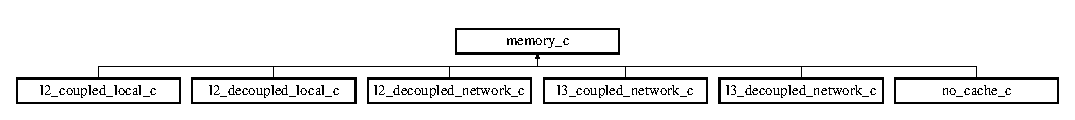
\includegraphics[height=1.159420cm]{classmemory__c}
\end{center}
\end{figure}
\subsection*{Public Member Functions}
\begin{DoxyCompactItemize}
\item 
\hypertarget{classmemory__c_aa642409499551fb2be1e9c1073f1ae58}{
{\bfseries memory\_\-c} (\hyperlink{classmacsim__c}{macsim\_\-c} $\ast$simBase)}
\label{classmemory__c_aa642409499551fb2be1e9c1073f1ae58}

\item 
bool \hyperlink{classmemory__c_ae7d66a0d0b90fd734cd568e238d626ea}{new\_\-mem\_\-req} (Mem\_\-Req\_\-Type type, Addr addr, uns size, uns delay, \hyperlink{classuop__c}{uop\_\-c} $\ast$uop, function$<$ bool(\hyperlink{structmem__req__s}{mem\_\-req\_\-s} $\ast$)$>$ done\_\-func, Counter unique\_\-num, \hyperlink{structpref__req__info__s}{pref\_\-req\_\-info\_\-s} $\ast$pref\_\-info, int core\_\-id, int thread\_\-id, bool ptx)
\item 
int \hyperlink{classmemory__c_ae4385c1817139c78c385339de8a90454}{access} (\hyperlink{classuop__c}{uop\_\-c} $\ast$uop)
\item 
Addr \hyperlink{classmemory__c_aca226079ad178cfcd5724d8b24ec937f}{base\_\-addr} (int core\_\-id, Addr addr)
\item 
int \hyperlink{classmemory__c_a70e1ed0c249016cfab45bfa2ce9a02a7}{line\_\-size} (int core\_\-id)
\item 
int \hyperlink{classmemory__c_afd93c2187e5879151868b3910dbfd99b}{bank\_\-id} (int core\_\-id, Addr addr)
\item 
bool \hyperlink{classmemory__c_a4b10208dda24728f314aa841107c8149}{get\_\-read\_\-port} (int core\_\-id, int bank\_\-id)
\item 
void \hyperlink{classmemory__c_a8663ad14c52686bcb441a55a8bcedc9a}{run\_\-a\_\-cycle} (void)
\item 
void \hyperlink{classmemory__c_a5bca39b03fc329e94230dc84b5649807}{free\_\-req} (int core\_\-id, \hyperlink{structmem__req__s}{mem\_\-req\_\-s} $\ast$req)
\item 
bool \hyperlink{classmemory__c_a64e019e7a18841fa0bb4136c1ce2f7cb}{receive} (int src, int dst, int msg, \hyperlink{structmem__req__s}{mem\_\-req\_\-s} $\ast$req)
\item 
int \hyperlink{classmemory__c_a2c7648ced944361742f1599c30a88e9a}{get\_\-dst\_\-id} (int level, int id)
\item 
int \hyperlink{classmemory__c_af80eff0db7549c4d1f267c608feb65ca}{get\_\-dst\_\-router\_\-id} (int level, int id)
\item 
void \hyperlink{classmemory__c_a37f7bb4a39885372fec26efa24927af9}{get\_\-level\_\-id} (int noc\_\-id, int $\ast$level, int $\ast$id)
\item 
bool \hyperlink{classmemory__c_ab0e78e319360a553d3e9864136176ccb}{done} (\hyperlink{structmem__req__s}{mem\_\-req\_\-s} $\ast$req)
\item 
\hyperlink{structdcache__data__s}{dcache\_\-data\_\-s} $\ast$ \hyperlink{classmemory__c_af3cabc34471d4d2af230f86f19799d0d}{access\_\-cache} (int core\_\-id, Addr addr, Addr $\ast$line\_\-addr, bool update, int appl\_\-id)
\item 
\hyperlink{structmem__req__s}{mem\_\-req\_\-s} $\ast$ \hyperlink{classmemory__c_a1fe0c501966e1ce43d8fdf6453031c37}{new\_\-wb\_\-req} (Addr addr, int size, bool ptx, \hyperlink{structdcache__data__s}{dcache\_\-data\_\-s} $\ast$data, int level)
\item 
void \hyperlink{classmemory__c_afbfb221d9819b83cc2807b7e539787f6}{print\_\-mshr} (void)
\item 
int \hyperlink{classmemory__c_a5d51af45787095c6453feb810302fd10}{get\_\-num\_\-avail\_\-entry} (int core\_\-id)
\item 
void \hyperlink{classmemory__c_ac244e4897309b864afa535d39e0b61a9}{init} (void)
\item 
\hypertarget{classmemory__c_aea2bbd7d03efed00e880ea6660487964}{
void {\bfseries handle\_\-coherence} (int level, bool hit, bool store, Addr addr, \hyperlink{classdcu__c}{dcu\_\-c} $\ast$cache)}
\label{classmemory__c_aea2bbd7d03efed00e880ea6660487964}

\end{DoxyCompactItemize}
\subsection*{Public Attributes}
\begin{DoxyCompactItemize}
\item 
int $\ast$ \hyperlink{classmemory__c_ad2743072864011245a46ee7038df5ae8}{m\_\-iris\_\-node\_\-id}
\end{DoxyCompactItemize}
\subsection*{Static Public Attributes}
\begin{DoxyCompactItemize}
\item 
static int \hyperlink{classmemory__c_a69b0fb5c2a19b6a196e86d1842a8a8a8}{m\_\-unique\_\-id} = 0
\end{DoxyCompactItemize}
\subsection*{Protected Member Functions}
\begin{DoxyCompactItemize}
\item 
\hyperlink{structmem__req__s}{mem\_\-req\_\-s} $\ast$ \hyperlink{classmemory__c_a57f0cd07a859cf117bf195cddadfebb3}{allocate\_\-new\_\-entry} (int core\_\-id)
\item 
void \hyperlink{classmemory__c_aea4d542da14dfc9d59d108e2cae665bb}{init\_\-new\_\-req} (\hyperlink{structmem__req__s}{mem\_\-req\_\-s} $\ast$req, Mem\_\-Req\_\-Type type, Addr addr, int size, int delay, \hyperlink{classuop__c}{uop\_\-c} $\ast$uop, function$<$ bool(\hyperlink{structmem__req__s}{mem\_\-req\_\-s} $\ast$)$>$ done\_\-func, Counter unique\_\-num, Counter priority, int core\_\-id, int thread\_\-id, bool ptx)
\item 
void \hyperlink{classmemory__c_ac3a3a9028dc3577a577c959e5256b38d}{adjust\_\-req} (\hyperlink{structmem__req__s}{mem\_\-req\_\-s} $\ast$req, Mem\_\-Req\_\-Type type, Addr addr, int size, int delay, \hyperlink{classuop__c}{uop\_\-c} $\ast$uop, function$<$ bool(\hyperlink{structmem__req__s}{mem\_\-req\_\-s} $\ast$)$>$ done\_\-func, Counter unique\_\-num, Counter priority, int core\_\-id, int thread\_\-id, bool ptx)
\item 
\hyperlink{structmem__req__s}{mem\_\-req\_\-s} $\ast$ \hyperlink{classmemory__c_aebf82c8ad5dbd9bbda629f0677be0c31}{search\_\-req} (int core\_\-id, Addr addr, int size)
\item 
virtual void \hyperlink{classmemory__c_aa15a04b3d5bb8e6ab0b7274b9c50a319}{set\_\-cache\_\-id} (\hyperlink{structmem__req__s}{mem\_\-req\_\-s} $\ast$req)
\item 
\hyperlink{structmem__req__s}{mem\_\-req\_\-s} $\ast$ \hyperlink{classmemory__c_aa2d744d2895b71290ec9475c6faa5640}{evict\_\-prefetch} (int core\_\-id)
\item 
void \hyperlink{classmemory__c_a5dc85d0815f9ebbcf69f4f85845dcb57}{flush\_\-prefetch} (int core\_\-id)
\end{DoxyCompactItemize}
\subsection*{Protected Attributes}
\begin{DoxyCompactItemize}
\item 
\hyperlink{classdcu__c}{dcu\_\-c} $\ast$$\ast$ \hyperlink{classmemory__c_a0bfafc54e9761b2ea991e668efb274c2}{m\_\-l1\_\-cache}
\item 
\hyperlink{classdcu__c}{dcu\_\-c} $\ast$$\ast$ \hyperlink{classmemory__c_a3d8dc521d1b278422bbc42a2a2ef446e}{m\_\-l2\_\-cache}
\item 
\hyperlink{classdcu__c}{dcu\_\-c} $\ast$$\ast$ \hyperlink{classmemory__c_a3ec227755e32dad0987dc9f6ec6681fd}{m\_\-l3\_\-cache}
\item 
\hyperlink{classdram__controller__c}{dram\_\-controller\_\-c} $\ast$$\ast$ \hyperlink{classmemory__c_a7372570a1fb983f16253261193a052bf}{m\_\-dram\_\-controller}
\item 
list$<$ \hyperlink{structmem__req__s}{mem\_\-req\_\-s} $\ast$ $>$ $\ast$ \hyperlink{classmemory__c_ab7b175ea316a51ff771ca652c2dae138}{m\_\-mshr}
\item 
list$<$ \hyperlink{structmem__req__s}{mem\_\-req\_\-s} $\ast$ $>$ $\ast$ \hyperlink{classmemory__c_a4268b16bf6a1f84172fc1a313a8f44c2}{m\_\-mshr\_\-free\_\-list}
\item 
int \hyperlink{classmemory__c_afaf8b643ce736f9ea9b2050b6740e710}{m\_\-num\_\-core}
\item 
int \hyperlink{classmemory__c_a3cf6fe78e2b25f56b3ff51b6f8b383d7}{m\_\-num\_\-l3}
\item 
int \hyperlink{classmemory__c_ade8ecba4b6abbf18ea424e530d0962e9}{m\_\-num\_\-mc}
\item 
int \hyperlink{classmemory__c_a1bf57a0de8f321201f37c448f7f730e7}{m\_\-noc\_\-index\_\-base} \mbox{[}MEM\_\-LAST\mbox{]}
\item 
int \hyperlink{classmemory__c_a7688509a181e0fd29dc6d70f59920f59}{m\_\-noc\_\-id\_\-base} \mbox{[}MEM\_\-LAST\mbox{]}
\item 
Counter \hyperlink{classmemory__c_ac90f740154b2099375a4464a264c3dc0}{m\_\-stop\_\-prefetch}
\item 
int \hyperlink{classmemory__c_abcf822c7e709f6013963173b5a8f6041}{m\_\-l3\_\-interleave\_\-factor}
\item 
\hyperlink{classmacsim__c}{macsim\_\-c} $\ast$ \hyperlink{classmemory__c_a8ba3319a3e385a0984dcb0ff7531a397}{m\_\-simBase}
\item 
unordered\_\-map$<$ Addr, vector$<$ bool $>$ $\ast$ $>$ \hyperlink{classmemory__c_ab6ce4ddeb85e8798bb9d844e6b2d6941}{m\_\-tag\_\-directory}
\item 
unordered\_\-map$<$ Addr, bool $>$ \hyperlink{classmemory__c_a4955ca08d109aa65c8532a1488dfffbb}{m\_\-td\_\-pending\_\-req}
\end{DoxyCompactItemize}


\subsection{Detailed Description}
memory system 

\subsection{Member Function Documentation}
\hypertarget{classmemory__c_ae4385c1817139c78c385339de8a90454}{
\index{memory\_\-c@{memory\_\-c}!access@{access}}
\index{access@{access}!memory_c@{memory\_\-c}}
\subsubsection[{access}]{\setlength{\rightskip}{0pt plus 5cm}int memory\_\-c::access (
\begin{DoxyParamCaption}
\item[{{\bf uop\_\-c} $\ast$}]{ uop}
\end{DoxyParamCaption}
)}}
\label{classmemory__c_ae4385c1817139c78c385339de8a90454}
Access first-\/level cache from execution stage \begin{DoxyReturn}{Returns}
0, if not accessed correctly 

-\/1, generate a new memory request 

L1\_\-latency, if hit 
\end{DoxyReturn}
\hypertarget{classmemory__c_af3cabc34471d4d2af230f86f19799d0d}{
\index{memory\_\-c@{memory\_\-c}!access\_\-cache@{access\_\-cache}}
\index{access\_\-cache@{access\_\-cache}!memory_c@{memory\_\-c}}
\subsubsection[{access\_\-cache}]{\setlength{\rightskip}{0pt plus 5cm}{\bf dcache\_\-data\_\-s} $\ast$ memory\_\-c::access\_\-cache (
\begin{DoxyParamCaption}
\item[{int}]{ core\_\-id, }
\item[{Addr}]{ addr, }
\item[{Addr $\ast$}]{ line\_\-addr, }
\item[{bool}]{ update, }
\item[{int}]{ appl\_\-id}
\end{DoxyParamCaption}
)}}
\label{classmemory__c_af3cabc34471d4d2af230f86f19799d0d}
Access L1 data cache \hypertarget{classmemory__c_ac3a3a9028dc3577a577c959e5256b38d}{
\index{memory\_\-c@{memory\_\-c}!adjust\_\-req@{adjust\_\-req}}
\index{adjust\_\-req@{adjust\_\-req}!memory_c@{memory\_\-c}}
\subsubsection[{adjust\_\-req}]{\setlength{\rightskip}{0pt plus 5cm}void memory\_\-c::adjust\_\-req (
\begin{DoxyParamCaption}
\item[{{\bf mem\_\-req\_\-s} $\ast$}]{ req, }
\item[{Mem\_\-Req\_\-Type}]{ type, }
\item[{Addr}]{ addr, }
\item[{int}]{ size, }
\item[{int}]{ delay, }
\item[{{\bf uop\_\-c} $\ast$}]{ uop, }
\item[{function$<$ bool({\bf mem\_\-req\_\-s} $\ast$)$>$}]{ done\_\-func, }
\item[{Counter}]{ unique\_\-num, }
\item[{Counter}]{ priority, }
\item[{int}]{ core\_\-id, }
\item[{int}]{ thread\_\-id, }
\item[{bool}]{ ptx}
\end{DoxyParamCaption}
)\hspace{0.3cm}{\ttfamily  \mbox{[}protected\mbox{]}}}}
\label{classmemory__c_ac3a3a9028dc3577a577c959e5256b38d}
Adjust a new request. In case of finding matching entry, we need to adjust fields of the matching request \hypertarget{classmemory__c_a57f0cd07a859cf117bf195cddadfebb3}{
\index{memory\_\-c@{memory\_\-c}!allocate\_\-new\_\-entry@{allocate\_\-new\_\-entry}}
\index{allocate\_\-new\_\-entry@{allocate\_\-new\_\-entry}!memory_c@{memory\_\-c}}
\subsubsection[{allocate\_\-new\_\-entry}]{\setlength{\rightskip}{0pt plus 5cm}{\bf mem\_\-req\_\-s} $\ast$ memory\_\-c::allocate\_\-new\_\-entry (
\begin{DoxyParamCaption}
\item[{int}]{ core\_\-id}
\end{DoxyParamCaption}
)\hspace{0.3cm}{\ttfamily  \mbox{[}protected\mbox{]}}}}
\label{classmemory__c_a57f0cd07a859cf117bf195cddadfebb3}
Allocate a new request from free list \hypertarget{classmemory__c_afd93c2187e5879151868b3910dbfd99b}{
\index{memory\_\-c@{memory\_\-c}!bank\_\-id@{bank\_\-id}}
\index{bank\_\-id@{bank\_\-id}!memory_c@{memory\_\-c}}
\subsubsection[{bank\_\-id}]{\setlength{\rightskip}{0pt plus 5cm}int memory\_\-c::bank\_\-id (
\begin{DoxyParamCaption}
\item[{int}]{ core\_\-id, }
\item[{Addr}]{ addr}
\end{DoxyParamCaption}
)}}
\label{classmemory__c_afd93c2187e5879151868b3910dbfd99b}
Return cache bank id \hypertarget{classmemory__c_aca226079ad178cfcd5724d8b24ec937f}{
\index{memory\_\-c@{memory\_\-c}!base\_\-addr@{base\_\-addr}}
\index{base\_\-addr@{base\_\-addr}!memory_c@{memory\_\-c}}
\subsubsection[{base\_\-addr}]{\setlength{\rightskip}{0pt plus 5cm}Addr memory\_\-c::base\_\-addr (
\begin{DoxyParamCaption}
\item[{int}]{ core\_\-id, }
\item[{Addr}]{ addr}
\end{DoxyParamCaption}
)}}
\label{classmemory__c_aca226079ad178cfcd5724d8b24ec937f}
Return base line address \hypertarget{classmemory__c_ab0e78e319360a553d3e9864136176ccb}{
\index{memory\_\-c@{memory\_\-c}!done@{done}}
\index{done@{done}!memory_c@{memory\_\-c}}
\subsubsection[{done}]{\setlength{\rightskip}{0pt plus 5cm}bool memory\_\-c::done (
\begin{DoxyParamCaption}
\item[{{\bf mem\_\-req\_\-s} $\ast$}]{ req}
\end{DoxyParamCaption}
)}}
\label{classmemory__c_ab0e78e319360a553d3e9864136176ccb}
Cache line fill function \hypertarget{classmemory__c_aa2d744d2895b71290ec9475c6faa5640}{
\index{memory\_\-c@{memory\_\-c}!evict\_\-prefetch@{evict\_\-prefetch}}
\index{evict\_\-prefetch@{evict\_\-prefetch}!memory_c@{memory\_\-c}}
\subsubsection[{evict\_\-prefetch}]{\setlength{\rightskip}{0pt plus 5cm}{\bf mem\_\-req\_\-s} $\ast$ memory\_\-c::evict\_\-prefetch (
\begin{DoxyParamCaption}
\item[{int}]{ core\_\-id}
\end{DoxyParamCaption}
)\hspace{0.3cm}{\ttfamily  \mbox{[}protected\mbox{]}}}}
\label{classmemory__c_aa2d744d2895b71290ec9475c6faa5640}
When MSHR is full, try to evict a prefetch request \hypertarget{classmemory__c_a5dc85d0815f9ebbcf69f4f85845dcb57}{
\index{memory\_\-c@{memory\_\-c}!flush\_\-prefetch@{flush\_\-prefetch}}
\index{flush\_\-prefetch@{flush\_\-prefetch}!memory_c@{memory\_\-c}}
\subsubsection[{flush\_\-prefetch}]{\setlength{\rightskip}{0pt plus 5cm}void memory\_\-c::flush\_\-prefetch (
\begin{DoxyParamCaption}
\item[{int}]{ core\_\-id}
\end{DoxyParamCaption}
)\hspace{0.3cm}{\ttfamily  \mbox{[}protected\mbox{]}}}}
\label{classmemory__c_a5dc85d0815f9ebbcf69f4f85845dcb57}
Flush all prefetches in MSHR \hypertarget{classmemory__c_a5bca39b03fc329e94230dc84b5649807}{
\index{memory\_\-c@{memory\_\-c}!free\_\-req@{free\_\-req}}
\index{free\_\-req@{free\_\-req}!memory_c@{memory\_\-c}}
\subsubsection[{free\_\-req}]{\setlength{\rightskip}{0pt plus 5cm}void memory\_\-c::free\_\-req (
\begin{DoxyParamCaption}
\item[{int}]{ core\_\-id, }
\item[{{\bf mem\_\-req\_\-s} $\ast$}]{ req}
\end{DoxyParamCaption}
)}}
\label{classmemory__c_a5bca39b03fc329e94230dc84b5649807}
Deallocate completed memory request \hypertarget{classmemory__c_a2c7648ced944361742f1599c30a88e9a}{
\index{memory\_\-c@{memory\_\-c}!get\_\-dst\_\-id@{get\_\-dst\_\-id}}
\index{get\_\-dst\_\-id@{get\_\-dst\_\-id}!memory_c@{memory\_\-c}}
\subsubsection[{get\_\-dst\_\-id}]{\setlength{\rightskip}{0pt plus 5cm}int memory\_\-c::get\_\-dst\_\-id (
\begin{DoxyParamCaption}
\item[{int}]{ level, }
\item[{int}]{ id}
\end{DoxyParamCaption}
)}}
\label{classmemory__c_a2c7648ced944361742f1599c30a88e9a}
Using level and its id, get network id \hypertarget{classmemory__c_af80eff0db7549c4d1f267c608feb65ca}{
\index{memory\_\-c@{memory\_\-c}!get\_\-dst\_\-router\_\-id@{get\_\-dst\_\-router\_\-id}}
\index{get\_\-dst\_\-router\_\-id@{get\_\-dst\_\-router\_\-id}!memory_c@{memory\_\-c}}
\subsubsection[{get\_\-dst\_\-router\_\-id}]{\setlength{\rightskip}{0pt plus 5cm}int memory\_\-c::get\_\-dst\_\-router\_\-id (
\begin{DoxyParamCaption}
\item[{int}]{ level, }
\item[{int}]{ id}
\end{DoxyParamCaption}
)}}
\label{classmemory__c_af80eff0db7549c4d1f267c608feb65ca}
Using level and its id, get destination router id \hypertarget{classmemory__c_a37f7bb4a39885372fec26efa24927af9}{
\index{memory\_\-c@{memory\_\-c}!get\_\-level\_\-id@{get\_\-level\_\-id}}
\index{get\_\-level\_\-id@{get\_\-level\_\-id}!memory_c@{memory\_\-c}}
\subsubsection[{get\_\-level\_\-id}]{\setlength{\rightskip}{0pt plus 5cm}void memory\_\-c::get\_\-level\_\-id (
\begin{DoxyParamCaption}
\item[{int}]{ noc\_\-id, }
\item[{int $\ast$}]{ level, }
\item[{int $\ast$}]{ id}
\end{DoxyParamCaption}
)}}
\label{classmemory__c_a37f7bb4a39885372fec26efa24927af9}
Using network id, get level and its id \hypertarget{classmemory__c_a5d51af45787095c6453feb810302fd10}{
\index{memory\_\-c@{memory\_\-c}!get\_\-num\_\-avail\_\-entry@{get\_\-num\_\-avail\_\-entry}}
\index{get\_\-num\_\-avail\_\-entry@{get\_\-num\_\-avail\_\-entry}!memory_c@{memory\_\-c}}
\subsubsection[{get\_\-num\_\-avail\_\-entry}]{\setlength{\rightskip}{0pt plus 5cm}int memory\_\-c::get\_\-num\_\-avail\_\-entry (
\begin{DoxyParamCaption}
\item[{int}]{ core\_\-id}
\end{DoxyParamCaption}
)}}
\label{classmemory__c_a5d51af45787095c6453feb810302fd10}
Check available entry in mshr \hypertarget{classmemory__c_a4b10208dda24728f314aa841107c8149}{
\index{memory\_\-c@{memory\_\-c}!get\_\-read\_\-port@{get\_\-read\_\-port}}
\index{get\_\-read\_\-port@{get\_\-read\_\-port}!memory_c@{memory\_\-c}}
\subsubsection[{get\_\-read\_\-port}]{\setlength{\rightskip}{0pt plus 5cm}bool memory\_\-c::get\_\-read\_\-port (
\begin{DoxyParamCaption}
\item[{int}]{ core\_\-id, }
\item[{int}]{ bank\_\-id}
\end{DoxyParamCaption}
)}}
\label{classmemory__c_a4b10208dda24728f314aa841107c8149}
Acquire dcache read port with the specified bank \hypertarget{classmemory__c_ac244e4897309b864afa535d39e0b61a9}{
\index{memory\_\-c@{memory\_\-c}!init@{init}}
\index{init@{init}!memory_c@{memory\_\-c}}
\subsubsection[{init}]{\setlength{\rightskip}{0pt plus 5cm}void memory\_\-c::init (
\begin{DoxyParamCaption}
\item[{void}]{}
\end{DoxyParamCaption}
)}}
\label{classmemory__c_ac244e4897309b864afa535d39e0b61a9}
Initialize the memory system. \par
 Setup interconnection network interface. \hypertarget{classmemory__c_aea4d542da14dfc9d59d108e2cae665bb}{
\index{memory\_\-c@{memory\_\-c}!init\_\-new\_\-req@{init\_\-new\_\-req}}
\index{init\_\-new\_\-req@{init\_\-new\_\-req}!memory_c@{memory\_\-c}}
\subsubsection[{init\_\-new\_\-req}]{\setlength{\rightskip}{0pt plus 5cm}void memory\_\-c::init\_\-new\_\-req (
\begin{DoxyParamCaption}
\item[{{\bf mem\_\-req\_\-s} $\ast$}]{ req, }
\item[{Mem\_\-Req\_\-Type}]{ type, }
\item[{Addr}]{ addr, }
\item[{int}]{ size, }
\item[{int}]{ delay, }
\item[{{\bf uop\_\-c} $\ast$}]{ uop, }
\item[{function$<$ bool({\bf mem\_\-req\_\-s} $\ast$)$>$}]{ done\_\-func, }
\item[{Counter}]{ unique\_\-num, }
\item[{Counter}]{ priority, }
\item[{int}]{ core\_\-id, }
\item[{int}]{ thread\_\-id, }
\item[{bool}]{ ptx}
\end{DoxyParamCaption}
)\hspace{0.3cm}{\ttfamily  \mbox{[}protected\mbox{]}}}}
\label{classmemory__c_aea4d542da14dfc9d59d108e2cae665bb}
Initialize a new request \hypertarget{classmemory__c_a70e1ed0c249016cfab45bfa2ce9a02a7}{
\index{memory\_\-c@{memory\_\-c}!line\_\-size@{line\_\-size}}
\index{line\_\-size@{line\_\-size}!memory_c@{memory\_\-c}}
\subsubsection[{line\_\-size}]{\setlength{\rightskip}{0pt plus 5cm}int memory\_\-c::line\_\-size (
\begin{DoxyParamCaption}
\item[{int}]{ core\_\-id}
\end{DoxyParamCaption}
)}}
\label{classmemory__c_a70e1ed0c249016cfab45bfa2ce9a02a7}
Return cache line size \hypertarget{classmemory__c_ae7d66a0d0b90fd734cd568e238d626ea}{
\index{memory\_\-c@{memory\_\-c}!new\_\-mem\_\-req@{new\_\-mem\_\-req}}
\index{new\_\-mem\_\-req@{new\_\-mem\_\-req}!memory_c@{memory\_\-c}}
\subsubsection[{new\_\-mem\_\-req}]{\setlength{\rightskip}{0pt plus 5cm}bool memory\_\-c::new\_\-mem\_\-req (
\begin{DoxyParamCaption}
\item[{Mem\_\-Req\_\-Type}]{ type, }
\item[{Addr}]{ addr, }
\item[{uns}]{ size, }
\item[{uns}]{ delay, }
\item[{{\bf uop\_\-c} $\ast$}]{ uop, }
\item[{function$<$ bool({\bf mem\_\-req\_\-s} $\ast$)$>$}]{ done\_\-func, }
\item[{Counter}]{ unique\_\-num, }
\item[{{\bf pref\_\-req\_\-info\_\-s} $\ast$}]{ pref\_\-info, }
\item[{int}]{ core\_\-id, }
\item[{int}]{ thread\_\-id, }
\item[{bool}]{ ptx}
\end{DoxyParamCaption}
)}}
\label{classmemory__c_ae7d66a0d0b90fd734cd568e238d626ea}
Generate a new memory request 
\begin{DoxyParams}{Parameters}
\item[{\em type}]-\/ memory request type \item[{\em addr}]-\/ memory request address \item[{\em size}]-\/ memory request size \item[{\em delay}]-\/ delay \item[{\em uop}]-\/ request generating uop \item[{\em done\_\-func}]-\/ done function \item[{\em unique\_\-num}]-\/ uop unique number \item[{\em pref\_\-info}]-\/ prefetch information structure \item[{\em core\_\-id}]-\/ core id \item[{\em thread\_\-id}]-\/ thread id \item[{\em ptx}]-\/ GPU request \end{DoxyParams}
\begin{DoxyReturn}{Returns}
false, if mshr full or l2 queue full 

true, otherwise 
\end{DoxyReturn}
\hypertarget{classmemory__c_a1fe0c501966e1ce43d8fdf6453031c37}{
\index{memory\_\-c@{memory\_\-c}!new\_\-wb\_\-req@{new\_\-wb\_\-req}}
\index{new\_\-wb\_\-req@{new\_\-wb\_\-req}!memory_c@{memory\_\-c}}
\subsubsection[{new\_\-wb\_\-req}]{\setlength{\rightskip}{0pt plus 5cm}{\bf mem\_\-req\_\-s} $\ast$ memory\_\-c::new\_\-wb\_\-req (
\begin{DoxyParamCaption}
\item[{Addr}]{ addr, }
\item[{int}]{ size, }
\item[{bool}]{ ptx, }
\item[{{\bf dcache\_\-data\_\-s} $\ast$}]{ data, }
\item[{int}]{ level}
\end{DoxyParamCaption}
)}}
\label{classmemory__c_a1fe0c501966e1ce43d8fdf6453031c37}
Generate a new write-\/back request \hypertarget{classmemory__c_afbfb221d9819b83cc2807b7e539787f6}{
\index{memory\_\-c@{memory\_\-c}!print\_\-mshr@{print\_\-mshr}}
\index{print\_\-mshr@{print\_\-mshr}!memory_c@{memory\_\-c}}
\subsubsection[{print\_\-mshr}]{\setlength{\rightskip}{0pt plus 5cm}void memory\_\-c::print\_\-mshr (
\begin{DoxyParamCaption}
\item[{void}]{}
\end{DoxyParamCaption}
)}}
\label{classmemory__c_afbfb221d9819b83cc2807b7e539787f6}
Print all entries in MSHR \hypertarget{classmemory__c_a64e019e7a18841fa0bb4136c1ce2f7cb}{
\index{memory\_\-c@{memory\_\-c}!receive@{receive}}
\index{receive@{receive}!memory_c@{memory\_\-c}}
\subsubsection[{receive}]{\setlength{\rightskip}{0pt plus 5cm}bool memory\_\-c::receive (
\begin{DoxyParamCaption}
\item[{int}]{ src, }
\item[{int}]{ dst, }
\item[{int}]{ msg, }
\item[{{\bf mem\_\-req\_\-s} $\ast$}]{ req}
\end{DoxyParamCaption}
)}}
\label{classmemory__c_a64e019e7a18841fa0bb4136c1ce2f7cb}
Receive a message from NoC \hypertarget{classmemory__c_a8663ad14c52686bcb441a55a8bcedc9a}{
\index{memory\_\-c@{memory\_\-c}!run\_\-a\_\-cycle@{run\_\-a\_\-cycle}}
\index{run\_\-a\_\-cycle@{run\_\-a\_\-cycle}!memory_c@{memory\_\-c}}
\subsubsection[{run\_\-a\_\-cycle}]{\setlength{\rightskip}{0pt plus 5cm}void memory\_\-c::run\_\-a\_\-cycle (
\begin{DoxyParamCaption}
\item[{void}]{}
\end{DoxyParamCaption}
)}}
\label{classmemory__c_a8663ad14c52686bcb441a55a8bcedc9a}
Tick a cycle for the memory system \hypertarget{classmemory__c_aebf82c8ad5dbd9bbda629f0677be0c31}{
\index{memory\_\-c@{memory\_\-c}!search\_\-req@{search\_\-req}}
\index{search\_\-req@{search\_\-req}!memory_c@{memory\_\-c}}
\subsubsection[{search\_\-req}]{\setlength{\rightskip}{0pt plus 5cm}{\bf mem\_\-req\_\-s} $\ast$ memory\_\-c::search\_\-req (
\begin{DoxyParamCaption}
\item[{int}]{ core\_\-id, }
\item[{Addr}]{ addr, }
\item[{int}]{ size}
\end{DoxyParamCaption}
)\hspace{0.3cm}{\ttfamily  \mbox{[}protected\mbox{]}}}}
\label{classmemory__c_aebf82c8ad5dbd9bbda629f0677be0c31}
Search a request from queues \hypertarget{classmemory__c_aa15a04b3d5bb8e6ab0b7274b9c50a319}{
\index{memory\_\-c@{memory\_\-c}!set\_\-cache\_\-id@{set\_\-cache\_\-id}}
\index{set\_\-cache\_\-id@{set\_\-cache\_\-id}!memory_c@{memory\_\-c}}
\subsubsection[{set\_\-cache\_\-id}]{\setlength{\rightskip}{0pt plus 5cm}void memory\_\-c::set\_\-cache\_\-id (
\begin{DoxyParamCaption}
\item[{{\bf mem\_\-req\_\-s} $\ast$}]{ req}
\end{DoxyParamCaption}
)\hspace{0.3cm}{\ttfamily  \mbox{[}protected, virtual\mbox{]}}}}
\label{classmemory__c_aa15a04b3d5bb8e6ab0b7274b9c50a319}
Set the level of each cache level 

Reimplemented in \hyperlink{classl2__coupled__local__c_a4f3ca72f4a2ee33fa7f8b97b21e72364}{l2\_\-coupled\_\-local\_\-c}, \hyperlink{classno__cache__c_aec1175eba0781322b067d5fa906391ed}{no\_\-cache\_\-c}, \hyperlink{classl2__decoupled__network__c_aea63c8492607041d4d3ab90c8fa2961e}{l2\_\-decoupled\_\-network\_\-c}, and \hyperlink{classl2__decoupled__local__c_a4c319b02982447d98079bf6649fa5c15}{l2\_\-decoupled\_\-local\_\-c}.



\subsection{Member Data Documentation}
\hypertarget{classmemory__c_a7372570a1fb983f16253261193a052bf}{
\index{memory\_\-c@{memory\_\-c}!m\_\-dram\_\-controller@{m\_\-dram\_\-controller}}
\index{m\_\-dram\_\-controller@{m\_\-dram\_\-controller}!memory_c@{memory\_\-c}}
\subsubsection[{m\_\-dram\_\-controller}]{\setlength{\rightskip}{0pt plus 5cm}{\bf dram\_\-controller\_\-c}$\ast$$\ast$ {\bf memory\_\-c::m\_\-dram\_\-controller}\hspace{0.3cm}{\ttfamily  \mbox{[}protected\mbox{]}}}}
\label{classmemory__c_a7372570a1fb983f16253261193a052bf}
dram controllers \hypertarget{classmemory__c_ad2743072864011245a46ee7038df5ae8}{
\index{memory\_\-c@{memory\_\-c}!m\_\-iris\_\-node\_\-id@{m\_\-iris\_\-node\_\-id}}
\index{m\_\-iris\_\-node\_\-id@{m\_\-iris\_\-node\_\-id}!memory_c@{memory\_\-c}}
\subsubsection[{m\_\-iris\_\-node\_\-id}]{\setlength{\rightskip}{0pt plus 5cm}int$\ast$ {\bf memory\_\-c::m\_\-iris\_\-node\_\-id}}}
\label{classmemory__c_ad2743072864011245a46ee7038df5ae8}
noc id for iris network nodes \hypertarget{classmemory__c_a0bfafc54e9761b2ea991e668efb274c2}{
\index{memory\_\-c@{memory\_\-c}!m\_\-l1\_\-cache@{m\_\-l1\_\-cache}}
\index{m\_\-l1\_\-cache@{m\_\-l1\_\-cache}!memory_c@{memory\_\-c}}
\subsubsection[{m\_\-l1\_\-cache}]{\setlength{\rightskip}{0pt plus 5cm}{\bf dcu\_\-c}$\ast$$\ast$ {\bf memory\_\-c::m\_\-l1\_\-cache}\hspace{0.3cm}{\ttfamily  \mbox{[}protected\mbox{]}}}}
\label{classmemory__c_a0bfafc54e9761b2ea991e668efb274c2}
L1 caches \hypertarget{classmemory__c_a3d8dc521d1b278422bbc42a2a2ef446e}{
\index{memory\_\-c@{memory\_\-c}!m\_\-l2\_\-cache@{m\_\-l2\_\-cache}}
\index{m\_\-l2\_\-cache@{m\_\-l2\_\-cache}!memory_c@{memory\_\-c}}
\subsubsection[{m\_\-l2\_\-cache}]{\setlength{\rightskip}{0pt plus 5cm}{\bf dcu\_\-c}$\ast$$\ast$ {\bf memory\_\-c::m\_\-l2\_\-cache}\hspace{0.3cm}{\ttfamily  \mbox{[}protected\mbox{]}}}}
\label{classmemory__c_a3d8dc521d1b278422bbc42a2a2ef446e}
L2 caches \hypertarget{classmemory__c_a3ec227755e32dad0987dc9f6ec6681fd}{
\index{memory\_\-c@{memory\_\-c}!m\_\-l3\_\-cache@{m\_\-l3\_\-cache}}
\index{m\_\-l3\_\-cache@{m\_\-l3\_\-cache}!memory_c@{memory\_\-c}}
\subsubsection[{m\_\-l3\_\-cache}]{\setlength{\rightskip}{0pt plus 5cm}{\bf dcu\_\-c}$\ast$$\ast$ {\bf memory\_\-c::m\_\-l3\_\-cache}\hspace{0.3cm}{\ttfamily  \mbox{[}protected\mbox{]}}}}
\label{classmemory__c_a3ec227755e32dad0987dc9f6ec6681fd}
L3 caches \hypertarget{classmemory__c_abcf822c7e709f6013963173b5a8f6041}{
\index{memory\_\-c@{memory\_\-c}!m\_\-l3\_\-interleave\_\-factor@{m\_\-l3\_\-interleave\_\-factor}}
\index{m\_\-l3\_\-interleave\_\-factor@{m\_\-l3\_\-interleave\_\-factor}!memory_c@{memory\_\-c}}
\subsubsection[{m\_\-l3\_\-interleave\_\-factor}]{\setlength{\rightskip}{0pt plus 5cm}int {\bf memory\_\-c::m\_\-l3\_\-interleave\_\-factor}\hspace{0.3cm}{\ttfamily  \mbox{[}protected\mbox{]}}}}
\label{classmemory__c_abcf822c7e709f6013963173b5a8f6041}
mask bit for L3 id \hypertarget{classmemory__c_ab7b175ea316a51ff771ca652c2dae138}{
\index{memory\_\-c@{memory\_\-c}!m\_\-mshr@{m\_\-mshr}}
\index{m\_\-mshr@{m\_\-mshr}!memory_c@{memory\_\-c}}
\subsubsection[{m\_\-mshr}]{\setlength{\rightskip}{0pt plus 5cm}list$<${\bf mem\_\-req\_\-s}$\ast$$>$$\ast$ {\bf memory\_\-c::m\_\-mshr}\hspace{0.3cm}{\ttfamily  \mbox{[}protected\mbox{]}}}}
\label{classmemory__c_ab7b175ea316a51ff771ca652c2dae138}
mshr entry per L1 cache \hypertarget{classmemory__c_a4268b16bf6a1f84172fc1a313a8f44c2}{
\index{memory\_\-c@{memory\_\-c}!m\_\-mshr\_\-free\_\-list@{m\_\-mshr\_\-free\_\-list}}
\index{m\_\-mshr\_\-free\_\-list@{m\_\-mshr\_\-free\_\-list}!memory_c@{memory\_\-c}}
\subsubsection[{m\_\-mshr\_\-free\_\-list}]{\setlength{\rightskip}{0pt plus 5cm}list$<${\bf mem\_\-req\_\-s}$\ast$$>$$\ast$ {\bf memory\_\-c::m\_\-mshr\_\-free\_\-list}\hspace{0.3cm}{\ttfamily  \mbox{[}protected\mbox{]}}}}
\label{classmemory__c_a4268b16bf6a1f84172fc1a313a8f44c2}
mshr entry free list \hypertarget{classmemory__c_a7688509a181e0fd29dc6d70f59920f59}{
\index{memory\_\-c@{memory\_\-c}!m\_\-noc\_\-id\_\-base@{m\_\-noc\_\-id\_\-base}}
\index{m\_\-noc\_\-id\_\-base@{m\_\-noc\_\-id\_\-base}!memory_c@{memory\_\-c}}
\subsubsection[{m\_\-noc\_\-id\_\-base}]{\setlength{\rightskip}{0pt plus 5cm}int {\bf memory\_\-c::m\_\-noc\_\-id\_\-base}\mbox{[}MEM\_\-LAST\mbox{]}\hspace{0.3cm}{\ttfamily  \mbox{[}protected\mbox{]}}}}
\label{classmemory__c_a7688509a181e0fd29dc6d70f59920f59}
noc id base per level \hypertarget{classmemory__c_a1bf57a0de8f321201f37c448f7f730e7}{
\index{memory\_\-c@{memory\_\-c}!m\_\-noc\_\-index\_\-base@{m\_\-noc\_\-index\_\-base}}
\index{m\_\-noc\_\-index\_\-base@{m\_\-noc\_\-index\_\-base}!memory_c@{memory\_\-c}}
\subsubsection[{m\_\-noc\_\-index\_\-base}]{\setlength{\rightskip}{0pt plus 5cm}int {\bf memory\_\-c::m\_\-noc\_\-index\_\-base}\mbox{[}MEM\_\-LAST\mbox{]}\hspace{0.3cm}{\ttfamily  \mbox{[}protected\mbox{]}}}}
\label{classmemory__c_a1bf57a0de8f321201f37c448f7f730e7}
component id of each memory hierarchy \hypertarget{classmemory__c_afaf8b643ce736f9ea9b2050b6740e710}{
\index{memory\_\-c@{memory\_\-c}!m\_\-num\_\-core@{m\_\-num\_\-core}}
\index{m\_\-num\_\-core@{m\_\-num\_\-core}!memory_c@{memory\_\-c}}
\subsubsection[{m\_\-num\_\-core}]{\setlength{\rightskip}{0pt plus 5cm}int {\bf memory\_\-c::m\_\-num\_\-core}\hspace{0.3cm}{\ttfamily  \mbox{[}protected\mbox{]}}}}
\label{classmemory__c_afaf8b643ce736f9ea9b2050b6740e710}
number of cores \hypertarget{classmemory__c_a3cf6fe78e2b25f56b3ff51b6f8b383d7}{
\index{memory\_\-c@{memory\_\-c}!m\_\-num\_\-l3@{m\_\-num\_\-l3}}
\index{m\_\-num\_\-l3@{m\_\-num\_\-l3}!memory_c@{memory\_\-c}}
\subsubsection[{m\_\-num\_\-l3}]{\setlength{\rightskip}{0pt plus 5cm}int {\bf memory\_\-c::m\_\-num\_\-l3}\hspace{0.3cm}{\ttfamily  \mbox{[}protected\mbox{]}}}}
\label{classmemory__c_a3cf6fe78e2b25f56b3ff51b6f8b383d7}
number of l3 caches \hypertarget{classmemory__c_ade8ecba4b6abbf18ea424e530d0962e9}{
\index{memory\_\-c@{memory\_\-c}!m\_\-num\_\-mc@{m\_\-num\_\-mc}}
\index{m\_\-num\_\-mc@{m\_\-num\_\-mc}!memory_c@{memory\_\-c}}
\subsubsection[{m\_\-num\_\-mc}]{\setlength{\rightskip}{0pt plus 5cm}int {\bf memory\_\-c::m\_\-num\_\-mc}\hspace{0.3cm}{\ttfamily  \mbox{[}protected\mbox{]}}}}
\label{classmemory__c_ade8ecba4b6abbf18ea424e530d0962e9}
number of memory controllers \hypertarget{classmemory__c_a8ba3319a3e385a0984dcb0ff7531a397}{
\index{memory\_\-c@{memory\_\-c}!m\_\-simBase@{m\_\-simBase}}
\index{m\_\-simBase@{m\_\-simBase}!memory_c@{memory\_\-c}}
\subsubsection[{m\_\-simBase}]{\setlength{\rightskip}{0pt plus 5cm}{\bf macsim\_\-c}$\ast$ {\bf memory\_\-c::m\_\-simBase}\hspace{0.3cm}{\ttfamily  \mbox{[}protected\mbox{]}}}}
\label{classmemory__c_a8ba3319a3e385a0984dcb0ff7531a397}
\hyperlink{classmacsim__c}{macsim\_\-c} base class for simulation globals \hypertarget{classmemory__c_ac90f740154b2099375a4464a264c3dc0}{
\index{memory\_\-c@{memory\_\-c}!m\_\-stop\_\-prefetch@{m\_\-stop\_\-prefetch}}
\index{m\_\-stop\_\-prefetch@{m\_\-stop\_\-prefetch}!memory_c@{memory\_\-c}}
\subsubsection[{m\_\-stop\_\-prefetch}]{\setlength{\rightskip}{0pt plus 5cm}Counter {\bf memory\_\-c::m\_\-stop\_\-prefetch}\hspace{0.3cm}{\ttfamily  \mbox{[}protected\mbox{]}}}}
\label{classmemory__c_ac90f740154b2099375a4464a264c3dc0}
when set, no prefetches will be inserted \hypertarget{classmemory__c_ab6ce4ddeb85e8798bb9d844e6b2d6941}{
\index{memory\_\-c@{memory\_\-c}!m\_\-tag\_\-directory@{m\_\-tag\_\-directory}}
\index{m\_\-tag\_\-directory@{m\_\-tag\_\-directory}!memory_c@{memory\_\-c}}
\subsubsection[{m\_\-tag\_\-directory}]{\setlength{\rightskip}{0pt plus 5cm}unordered\_\-map$<$Addr, vector$<$bool$>$$\ast$$>$ {\bf memory\_\-c::m\_\-tag\_\-directory}\hspace{0.3cm}{\ttfamily  \mbox{[}protected\mbox{]}}}}
\label{classmemory__c_ab6ce4ddeb85e8798bb9d844e6b2d6941}
oracle cache coherence table \hypertarget{classmemory__c_a4955ca08d109aa65c8532a1488dfffbb}{
\index{memory\_\-c@{memory\_\-c}!m\_\-td\_\-pending\_\-req@{m\_\-td\_\-pending\_\-req}}
\index{m\_\-td\_\-pending\_\-req@{m\_\-td\_\-pending\_\-req}!memory_c@{memory\_\-c}}
\subsubsection[{m\_\-td\_\-pending\_\-req}]{\setlength{\rightskip}{0pt plus 5cm}unordered\_\-map$<$Addr, bool$>$ {\bf memory\_\-c::m\_\-td\_\-pending\_\-req}\hspace{0.3cm}{\ttfamily  \mbox{[}protected\mbox{]}}}}
\label{classmemory__c_a4955ca08d109aa65c8532a1488dfffbb}
pending requests in tag directory \hypertarget{classmemory__c_a69b0fb5c2a19b6a196e86d1842a8a8a8}{
\index{memory\_\-c@{memory\_\-c}!m\_\-unique\_\-id@{m\_\-unique\_\-id}}
\index{m\_\-unique\_\-id@{m\_\-unique\_\-id}!memory_c@{memory\_\-c}}
\subsubsection[{m\_\-unique\_\-id}]{\setlength{\rightskip}{0pt plus 5cm}int {\bf memory\_\-c::m\_\-unique\_\-id} = 0\hspace{0.3cm}{\ttfamily  \mbox{[}static\mbox{]}}}}
\label{classmemory__c_a69b0fb5c2a19b6a196e86d1842a8a8a8}
unique memory request id 

The documentation for this class was generated from the following files:\begin{DoxyCompactItemize}
\item 
memory.h\item 
memory.cc\end{DoxyCompactItemize}

\hypertarget{structmt__scheduler__s}{
\section{mt\_\-scheduler\_\-s Struct Reference}
\label{structmt__scheduler__s}\index{mt\_\-scheduler\_\-s@{mt\_\-scheduler\_\-s}}
}


Multi-\/Threading scheduler data structure.  




{\ttfamily \#include $<$frontend.h$>$}

\subsection*{Public Attributes}
\begin{DoxyCompactItemize}
\item 
Addr \hyperlink{structmt__scheduler__s_a8f5c01bc526c65e096e6b44d60c6d76f}{m\_\-fetch\_\-addr}
\item 
Addr \hyperlink{structmt__scheduler__s_a068da90109ff4cd4f00b184a5b74c07e}{m\_\-next\_\-fetch\_\-addr}
\end{DoxyCompactItemize}


\subsection{Detailed Description}
Multi-\/Threading scheduler data structure. 

\subsection{Member Data Documentation}
\hypertarget{structmt__scheduler__s_a8f5c01bc526c65e096e6b44d60c6d76f}{
\index{mt\_\-scheduler\_\-s@{mt\_\-scheduler\_\-s}!m\_\-fetch\_\-addr@{m\_\-fetch\_\-addr}}
\index{m\_\-fetch\_\-addr@{m\_\-fetch\_\-addr}!mt_scheduler_s@{mt\_\-scheduler\_\-s}}
\subsubsection[{m\_\-fetch\_\-addr}]{\setlength{\rightskip}{0pt plus 5cm}Addr {\bf mt\_\-scheduler\_\-s::m\_\-fetch\_\-addr}}}
\label{structmt__scheduler__s_a8f5c01bc526c65e096e6b44d60c6d76f}
current fetch address \hypertarget{structmt__scheduler__s_a068da90109ff4cd4f00b184a5b74c07e}{
\index{mt\_\-scheduler\_\-s@{mt\_\-scheduler\_\-s}!m\_\-next\_\-fetch\_\-addr@{m\_\-next\_\-fetch\_\-addr}}
\index{m\_\-next\_\-fetch\_\-addr@{m\_\-next\_\-fetch\_\-addr}!mt_scheduler_s@{mt\_\-scheduler\_\-s}}
\subsubsection[{m\_\-next\_\-fetch\_\-addr}]{\setlength{\rightskip}{0pt plus 5cm}Addr {\bf mt\_\-scheduler\_\-s::m\_\-next\_\-fetch\_\-addr}}}
\label{structmt__scheduler__s_a068da90109ff4cd4f00b184a5b74c07e}
next fetch address 

The documentation for this struct was generated from the following file:\begin{DoxyCompactItemize}
\item 
frontend.h\end{DoxyCompactItemize}

\hypertarget{classmulti__key__map__c}{
\section{multi\_\-key\_\-map\_\-c Class Reference}
\label{classmulti__key__map__c}\index{multi\_\-key\_\-map\_\-c@{multi\_\-key\_\-map\_\-c}}
}


hash with multiple keys  




{\ttfamily \#include $<$utils.h$>$}

\subsection*{Public Member Functions}
\begin{DoxyCompactItemize}
\item 
\hyperlink{classmulti__key__map__c_a10478aca09995a3572db5ece0f42b14b}{multi\_\-key\_\-map\_\-c} ()
\item 
\hyperlink{classmulti__key__map__c_abcce660edd4cc5d21b86b1efc61679cf}{$\sim$multi\_\-key\_\-map\_\-c} ()
\item 
int \hyperlink{classmulti__key__map__c_ab99cb6a05bb791560dca635328bee8a4}{find} (int key1, int key2)
\item 
int \hyperlink{classmulti__key__map__c_a71e80a3beb06b843f9ca94714e973ac3}{insert} (int key1, int key2)
\item 
\hypertarget{classmulti__key__map__c_a0e30025c7c55e3249f8e623054360d39}{
void {\bfseries delete\_\-table} (int key1)}
\label{classmulti__key__map__c_a0e30025c7c55e3249f8e623054360d39}

\end{DoxyCompactItemize}
\subsection*{Private Attributes}
\begin{DoxyCompactItemize}
\item 
unordered\_\-map$<$ int, unordered\_\-map$<$ int, int $>$ $\ast$ $>$ \hyperlink{classmulti__key__map__c_aba1b2934d007b3e4bd2c841c674b83e0}{m\_\-table}
\item 
int \hyperlink{classmulti__key__map__c_ad69aed9994fc585d4b4ef41f283995eb}{m\_\-size}
\end{DoxyCompactItemize}


\subsection{Detailed Description}
hash with multiple keys This class is used for remapping (application id, block id) to new unique block id. We need this feature to repeat same traces. 

\subsection{Constructor \& Destructor Documentation}
\hypertarget{classmulti__key__map__c_a10478aca09995a3572db5ece0f42b14b}{
\index{multi\_\-key\_\-map\_\-c@{multi\_\-key\_\-map\_\-c}!multi\_\-key\_\-map\_\-c@{multi\_\-key\_\-map\_\-c}}
\index{multi\_\-key\_\-map\_\-c@{multi\_\-key\_\-map\_\-c}!multi_key_map_c@{multi\_\-key\_\-map\_\-c}}
\subsubsection[{multi\_\-key\_\-map\_\-c}]{\setlength{\rightskip}{0pt plus 5cm}multi\_\-key\_\-map\_\-c::multi\_\-key\_\-map\_\-c (
\begin{DoxyParamCaption}
{}
\end{DoxyParamCaption}
)}}
\label{classmulti__key__map__c_a10478aca09995a3572db5ece0f42b14b}
Constructor \hypertarget{classmulti__key__map__c_abcce660edd4cc5d21b86b1efc61679cf}{
\index{multi\_\-key\_\-map\_\-c@{multi\_\-key\_\-map\_\-c}!$\sim$multi\_\-key\_\-map\_\-c@{$\sim$multi\_\-key\_\-map\_\-c}}
\index{$\sim$multi\_\-key\_\-map\_\-c@{$\sim$multi\_\-key\_\-map\_\-c}!multi_key_map_c@{multi\_\-key\_\-map\_\-c}}
\subsubsection[{$\sim$multi\_\-key\_\-map\_\-c}]{\setlength{\rightskip}{0pt plus 5cm}multi\_\-key\_\-map\_\-c::$\sim$multi\_\-key\_\-map\_\-c (
\begin{DoxyParamCaption}
{}
\end{DoxyParamCaption}
)}}
\label{classmulti__key__map__c_abcce660edd4cc5d21b86b1efc61679cf}
Destructor 

\subsection{Member Function Documentation}
\hypertarget{classmulti__key__map__c_ab99cb6a05bb791560dca635328bee8a4}{
\index{multi\_\-key\_\-map\_\-c@{multi\_\-key\_\-map\_\-c}!find@{find}}
\index{find@{find}!multi_key_map_c@{multi\_\-key\_\-map\_\-c}}
\subsubsection[{find}]{\setlength{\rightskip}{0pt plus 5cm}int multi\_\-key\_\-map\_\-c::find (
\begin{DoxyParamCaption}
\item[{int}]{ key1, }
\item[{int}]{ key2}
\end{DoxyParamCaption}
)}}
\label{classmulti__key__map__c_ab99cb6a05bb791560dca635328bee8a4}
Find an existing entry with two keys \hypertarget{classmulti__key__map__c_a71e80a3beb06b843f9ca94714e973ac3}{
\index{multi\_\-key\_\-map\_\-c@{multi\_\-key\_\-map\_\-c}!insert@{insert}}
\index{insert@{insert}!multi_key_map_c@{multi\_\-key\_\-map\_\-c}}
\subsubsection[{insert}]{\setlength{\rightskip}{0pt plus 5cm}int multi\_\-key\_\-map\_\-c::insert (
\begin{DoxyParamCaption}
\item[{int}]{ key1, }
\item[{int}]{ key2}
\end{DoxyParamCaption}
)}}
\label{classmulti__key__map__c_a71e80a3beb06b843f9ca94714e973ac3}
Insert a new entry with key1 and key2 

\subsection{Member Data Documentation}
\hypertarget{classmulti__key__map__c_ad69aed9994fc585d4b4ef41f283995eb}{
\index{multi\_\-key\_\-map\_\-c@{multi\_\-key\_\-map\_\-c}!m\_\-size@{m\_\-size}}
\index{m\_\-size@{m\_\-size}!multi_key_map_c@{multi\_\-key\_\-map\_\-c}}
\subsubsection[{m\_\-size}]{\setlength{\rightskip}{0pt plus 5cm}int {\bf multi\_\-key\_\-map\_\-c::m\_\-size}\hspace{0.3cm}{\ttfamily  \mbox{[}private\mbox{]}}}}
\label{classmulti__key__map__c_ad69aed9994fc585d4b4ef41f283995eb}
hash table size. to get unique id \hypertarget{classmulti__key__map__c_aba1b2934d007b3e4bd2c841c674b83e0}{
\index{multi\_\-key\_\-map\_\-c@{multi\_\-key\_\-map\_\-c}!m\_\-table@{m\_\-table}}
\index{m\_\-table@{m\_\-table}!multi_key_map_c@{multi\_\-key\_\-map\_\-c}}
\subsubsection[{m\_\-table}]{\setlength{\rightskip}{0pt plus 5cm}unordered\_\-map$<$int, unordered\_\-map$<$int, int$>$ $\ast$$>$ {\bf multi\_\-key\_\-map\_\-c::m\_\-table}\hspace{0.3cm}{\ttfamily  \mbox{[}private\mbox{]}}}}
\label{classmulti__key__map__c_aba1b2934d007b3e4bd2c841c674b83e0}
hash table 

The documentation for this class was generated from the following files:\begin{DoxyCompactItemize}
\item 
utils.h\item 
utils.cc\end{DoxyCompactItemize}

\hypertarget{classno__cache__c}{
\section{no\_\-cache\_\-c Class Reference}
\label{classno__cache__c}\index{no\_\-cache\_\-c@{no\_\-cache\_\-c}}
}


No cache architecture (NVIDIA G80, G200).  




{\ttfamily \#include $<$memory.h$>$}

Inheritance diagram for no\_\-cache\_\-c:\begin{figure}[H]
\begin{center}
\leavevmode
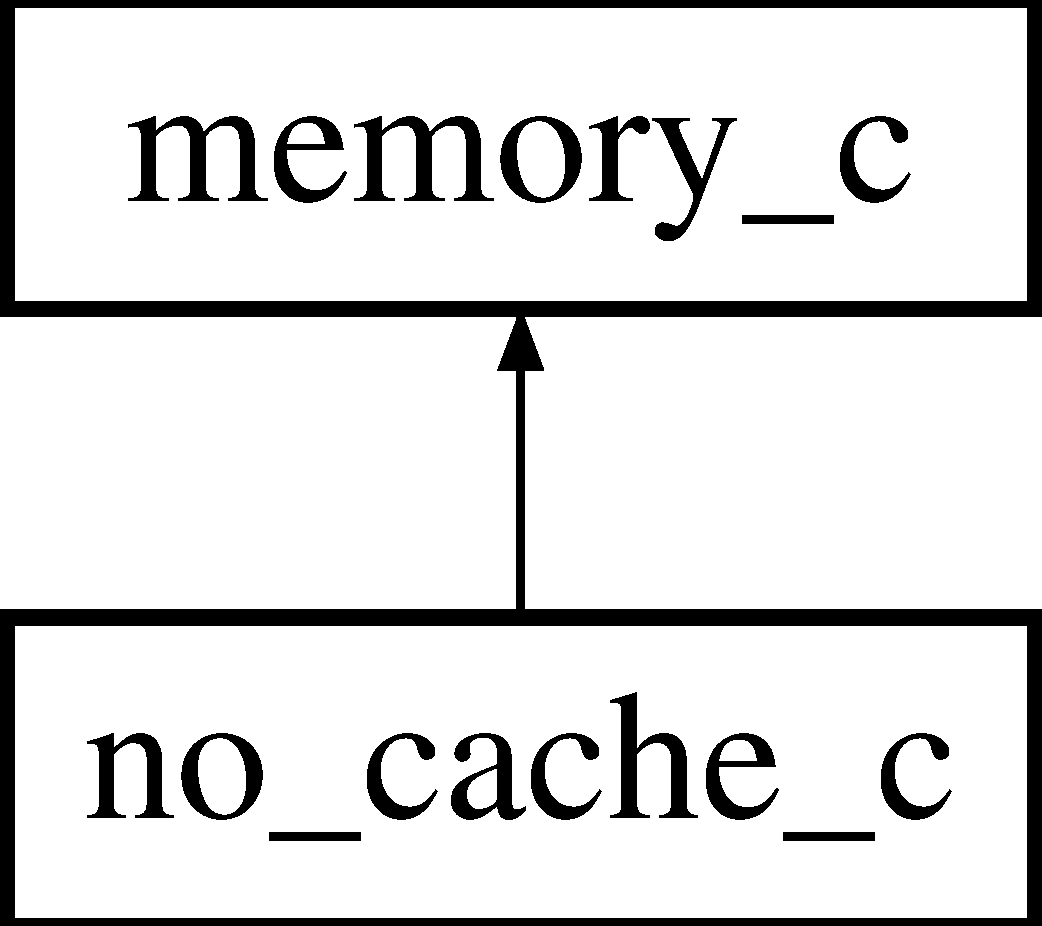
\includegraphics[height=2.000000cm]{classno__cache__c}
\end{center}
\end{figure}
\subsection*{Public Member Functions}
\begin{DoxyCompactItemize}
\item 
\hyperlink{classno__cache__c_a7326f78042de36c2d9436e9c481e5ec4}{no\_\-cache\_\-c} (\hyperlink{classmacsim__c}{macsim\_\-c} $\ast$simBase)
\item 
\hyperlink{classno__cache__c_aa6183a0375f657e152232a90879421c4}{$\sim$no\_\-cache\_\-c} ()
\end{DoxyCompactItemize}
\subsection*{Private Member Functions}
\begin{DoxyCompactItemize}
\item 
void \hyperlink{classno__cache__c_aec1175eba0781322b067d5fa906391ed}{set\_\-cache\_\-id} (\hyperlink{structmem__req__s}{mem\_\-req\_\-s} $\ast$req)
\end{DoxyCompactItemize}


\subsection{Detailed Description}
No cache architecture (NVIDIA G80, G200). 

\subsection{Constructor \& Destructor Documentation}
\hypertarget{classno__cache__c_a7326f78042de36c2d9436e9c481e5ec4}{
\index{no\_\-cache\_\-c@{no\_\-cache\_\-c}!no\_\-cache\_\-c@{no\_\-cache\_\-c}}
\index{no\_\-cache\_\-c@{no\_\-cache\_\-c}!no_cache_c@{no\_\-cache\_\-c}}
\subsubsection[{no\_\-cache\_\-c}]{\setlength{\rightskip}{0pt plus 5cm}no\_\-cache\_\-c::no\_\-cache\_\-c (
\begin{DoxyParamCaption}
\item[{{\bf macsim\_\-c} $\ast$}]{ simBase}
\end{DoxyParamCaption}
)}}
\label{classno__cache__c_a7326f78042de36c2d9436e9c481e5ec4}
Constructor \hypertarget{classno__cache__c_aa6183a0375f657e152232a90879421c4}{
\index{no\_\-cache\_\-c@{no\_\-cache\_\-c}!$\sim$no\_\-cache\_\-c@{$\sim$no\_\-cache\_\-c}}
\index{$\sim$no\_\-cache\_\-c@{$\sim$no\_\-cache\_\-c}!no_cache_c@{no\_\-cache\_\-c}}
\subsubsection[{$\sim$no\_\-cache\_\-c}]{\setlength{\rightskip}{0pt plus 5cm}no\_\-cache\_\-c::$\sim$no\_\-cache\_\-c (
\begin{DoxyParamCaption}
{}
\end{DoxyParamCaption}
)}}
\label{classno__cache__c_aa6183a0375f657e152232a90879421c4}
Destructor 

\subsection{Member Function Documentation}
\hypertarget{classno__cache__c_aec1175eba0781322b067d5fa906391ed}{
\index{no\_\-cache\_\-c@{no\_\-cache\_\-c}!set\_\-cache\_\-id@{set\_\-cache\_\-id}}
\index{set\_\-cache\_\-id@{set\_\-cache\_\-id}!no_cache_c@{no\_\-cache\_\-c}}
\subsubsection[{set\_\-cache\_\-id}]{\setlength{\rightskip}{0pt plus 5cm}void no\_\-cache\_\-c::set\_\-cache\_\-id (
\begin{DoxyParamCaption}
\item[{{\bf mem\_\-req\_\-s} $\ast$}]{ req}
\end{DoxyParamCaption}
)\hspace{0.3cm}{\ttfamily  \mbox{[}private, virtual\mbox{]}}}}
\label{classno__cache__c_aec1175eba0781322b067d5fa906391ed}
Set the level of each cache level 

Reimplemented from \hyperlink{classmemory__c_aa15a04b3d5bb8e6ab0b7274b9c50a319}{memory\_\-c}.



The documentation for this class was generated from the following files:\begin{DoxyCompactItemize}
\item 
memory.h\item 
memory.cc\end{DoxyCompactItemize}

\hypertarget{classnoc__c}{
\section{noc\_\-c Class Reference}
\label{classnoc__c}\index{noc\_\-c@{noc\_\-c}}
}


{\ttfamily \#include $<$noc.h$>$}

\subsection*{Public Member Functions}
\begin{DoxyCompactItemize}
\item 
\hyperlink{classnoc__c_a2556f3c8da43c1465d1c28f6d47a770e}{noc\_\-c} (\hyperlink{classmacsim__c}{macsim\_\-c} $\ast$simBase)
\item 
\hyperlink{classnoc__c_ad703b0eb1327952d067be27b68bcd27a}{$\sim$noc\_\-c} ()
\item 
bool \hyperlink{classnoc__c_a06803a1031a3a7a7a7067a25a702f52f}{insert} (int src, int dest, int msg, \hyperlink{structmem__req__s}{mem\_\-req\_\-s} $\ast$req)
\item 
void \hyperlink{classnoc__c_ae8caf32a2cbc114cc4c43ca1ee2113c5}{run\_\-a\_\-cycle} ()
\end{DoxyCompactItemize}
\subsection*{Private Attributes}
\begin{DoxyCompactItemize}
\item 
\hypertarget{classnoc__c_a347c2e3dcf9c5dfb97e5b3566f04fb24}{
\hyperlink{classmemory__c}{memory\_\-c} $\ast$ {\bfseries m\_\-memory}}
\label{classnoc__c_a347c2e3dcf9c5dfb97e5b3566f04fb24}

\item 
\hypertarget{classnoc__c_acdb2642b6945ebda3aae039b56f9372c}{
\hyperlink{classpool__c}{pool\_\-c}$<$ \hyperlink{structnoc__entry__s}{noc\_\-entry\_\-s} $>$ $\ast$ {\bfseries m\_\-pool}}
\label{classnoc__c_acdb2642b6945ebda3aae039b56f9372c}

\item 
\hypertarget{classnoc__c_a103461e69bbfded5d4d4f5bb82182957}{
list$<$ \hyperlink{structnoc__entry__s}{noc\_\-entry\_\-s} $\ast$ $>$ $\ast$ {\bfseries m\_\-cpu\_\-entry\_\-up}}
\label{classnoc__c_a103461e69bbfded5d4d4f5bb82182957}

\item 
\hypertarget{classnoc__c_a790a19529072e2f1717c136816350027}{
list$<$ \hyperlink{structnoc__entry__s}{noc\_\-entry\_\-s} $\ast$ $>$ $\ast$ {\bfseries m\_\-cpu\_\-entry\_\-down}}
\label{classnoc__c_a790a19529072e2f1717c136816350027}

\item 
\hypertarget{classnoc__c_a22800cde10b08f89ad96c8532aabc213}{
list$<$ \hyperlink{structnoc__entry__s}{noc\_\-entry\_\-s} $\ast$ $>$ $\ast$ {\bfseries m\_\-gpu\_\-entry\_\-up}}
\label{classnoc__c_a22800cde10b08f89ad96c8532aabc213}

\item 
\hypertarget{classnoc__c_a1e886512b84469d2d5735ebf7effb43b}{
list$<$ \hyperlink{structnoc__entry__s}{noc\_\-entry\_\-s} $\ast$ $>$ $\ast$ {\bfseries m\_\-gpu\_\-entry\_\-down}}
\label{classnoc__c_a1e886512b84469d2d5735ebf7effb43b}

\item 
\hyperlink{classmacsim__c}{macsim\_\-c} $\ast$ \hyperlink{classnoc__c_a2b62f87d3e010b3b935f16bf769db2bf}{m\_\-simBase}
\end{DoxyCompactItemize}


\subsection{Detailed Description}
NoC interface class 

\subsection{Constructor \& Destructor Documentation}
\hypertarget{classnoc__c_a2556f3c8da43c1465d1c28f6d47a770e}{
\index{noc\_\-c@{noc\_\-c}!noc\_\-c@{noc\_\-c}}
\index{noc\_\-c@{noc\_\-c}!noc_c@{noc\_\-c}}
\subsubsection[{noc\_\-c}]{\setlength{\rightskip}{0pt plus 5cm}noc\_\-c::noc\_\-c (
\begin{DoxyParamCaption}
\item[{{\bf macsim\_\-c} $\ast$}]{ simBase}
\end{DoxyParamCaption}
)}}
\label{classnoc__c_a2556f3c8da43c1465d1c28f6d47a770e}
NoC interface class constructor \hypertarget{classnoc__c_ad703b0eb1327952d067be27b68bcd27a}{
\index{noc\_\-c@{noc\_\-c}!$\sim$noc\_\-c@{$\sim$noc\_\-c}}
\index{$\sim$noc\_\-c@{$\sim$noc\_\-c}!noc_c@{noc\_\-c}}
\subsubsection[{$\sim$noc\_\-c}]{\setlength{\rightskip}{0pt plus 5cm}noc\_\-c::$\sim$noc\_\-c (
\begin{DoxyParamCaption}
{}
\end{DoxyParamCaption}
)}}
\label{classnoc__c_ad703b0eb1327952d067be27b68bcd27a}
NoC interface class destructor 

\subsection{Member Function Documentation}
\hypertarget{classnoc__c_a06803a1031a3a7a7a7067a25a702f52f}{
\index{noc\_\-c@{noc\_\-c}!insert@{insert}}
\index{insert@{insert}!noc_c@{noc\_\-c}}
\subsubsection[{insert}]{\setlength{\rightskip}{0pt plus 5cm}bool noc\_\-c::insert (
\begin{DoxyParamCaption}
\item[{int}]{ src, }
\item[{int}]{ dest, }
\item[{int}]{ msg, }
\item[{{\bf mem\_\-req\_\-s} $\ast$}]{ req}
\end{DoxyParamCaption}
)}}
\label{classnoc__c_a06803a1031a3a7a7a7067a25a702f52f}
Insert a new req/msg to the NoC \hypertarget{classnoc__c_ae8caf32a2cbc114cc4c43ca1ee2113c5}{
\index{noc\_\-c@{noc\_\-c}!run\_\-a\_\-cycle@{run\_\-a\_\-cycle}}
\index{run\_\-a\_\-cycle@{run\_\-a\_\-cycle}!noc_c@{noc\_\-c}}
\subsubsection[{run\_\-a\_\-cycle}]{\setlength{\rightskip}{0pt plus 5cm}void noc\_\-c::run\_\-a\_\-cycle (
\begin{DoxyParamCaption}
\item[{void}]{}
\end{DoxyParamCaption}
)}}
\label{classnoc__c_ae8caf32a2cbc114cc4c43ca1ee2113c5}
Tick a cycle 

\subsection{Member Data Documentation}
\hypertarget{classnoc__c_a2b62f87d3e010b3b935f16bf769db2bf}{
\index{noc\_\-c@{noc\_\-c}!m\_\-simBase@{m\_\-simBase}}
\index{m\_\-simBase@{m\_\-simBase}!noc_c@{noc\_\-c}}
\subsubsection[{m\_\-simBase}]{\setlength{\rightskip}{0pt plus 5cm}{\bf macsim\_\-c}$\ast$ {\bf noc\_\-c::m\_\-simBase}\hspace{0.3cm}{\ttfamily  \mbox{[}private\mbox{]}}}}
\label{classnoc__c_a2b62f87d3e010b3b935f16bf769db2bf}
\hyperlink{classmacsim__c}{macsim\_\-c} base class for simulation globals 

The documentation for this class was generated from the following files:\begin{DoxyCompactItemize}
\item 
noc.h\item 
noc.cc\end{DoxyCompactItemize}

\hypertarget{structnoc__entry__s}{
\section{noc\_\-entry\_\-s Struct Reference}
\label{structnoc__entry__s}\index{noc\_\-entry\_\-s@{noc\_\-entry\_\-s}}
}
\subsection*{Public Attributes}
\begin{DoxyCompactItemize}
\item 
\hypertarget{structnoc__entry__s_af8123088800fffd9ce505118436fcee8}{
int {\bfseries m\_\-src}}
\label{structnoc__entry__s_af8123088800fffd9ce505118436fcee8}

\item 
\hypertarget{structnoc__entry__s_a2904d8ce5478f5b7b9050e41b722ff42}{
int {\bfseries m\_\-dst}}
\label{structnoc__entry__s_a2904d8ce5478f5b7b9050e41b722ff42}

\item 
\hypertarget{structnoc__entry__s_a24e1182379a29649d6cb8ffb9bb65d9c}{
int {\bfseries m\_\-msg}}
\label{structnoc__entry__s_a24e1182379a29649d6cb8ffb9bb65d9c}

\item 
\hypertarget{structnoc__entry__s_a4472a1f9a73e12ce2fedb260ed5b5bf7}{
Counter {\bfseries m\_\-rdy}}
\label{structnoc__entry__s_a4472a1f9a73e12ce2fedb260ed5b5bf7}

\item 
\hypertarget{structnoc__entry__s_ab464d97cf14dfafbac20045c9609b13c}{
\hyperlink{structmem__req__s}{mem\_\-req\_\-s} $\ast$ {\bfseries m\_\-req}}
\label{structnoc__entry__s_ab464d97cf14dfafbac20045c9609b13c}

\end{DoxyCompactItemize}


The documentation for this struct was generated from the following file:\begin{DoxyCompactItemize}
\item 
noc.h\end{DoxyCompactItemize}

\hypertarget{structparam__file__entry__s}{
\section{param\_\-file\_\-entry\_\-s Struct Reference}
\label{structparam__file__entry__s}\index{param\_\-file\_\-entry\_\-s@{param\_\-file\_\-entry\_\-s}}
}


name and value of the knob from the file  




{\ttfamily \#include $<$knob.h$>$}

\subsection*{Public Attributes}
\begin{DoxyCompactItemize}
\item 
string \hyperlink{structparam__file__entry__s_ab6e7293d377cb8096750ab266ba0db3a}{m\_\-name}
\item 
string \hyperlink{structparam__file__entry__s_a6e496f0d5ce74bf6bf2602cd5e0f6472}{m\_\-value}
\end{DoxyCompactItemize}


\subsection{Detailed Description}
name and value of the knob from the file 

\subsection{Member Data Documentation}
\hypertarget{structparam__file__entry__s_ab6e7293d377cb8096750ab266ba0db3a}{
\index{param\_\-file\_\-entry\_\-s@{param\_\-file\_\-entry\_\-s}!m\_\-name@{m\_\-name}}
\index{m\_\-name@{m\_\-name}!param_file_entry_s@{param\_\-file\_\-entry\_\-s}}
\subsubsection[{m\_\-name}]{\setlength{\rightskip}{0pt plus 5cm}string {\bf param\_\-file\_\-entry\_\-s::m\_\-name}}}
\label{structparam__file__entry__s_ab6e7293d377cb8096750ab266ba0db3a}
knob name \hypertarget{structparam__file__entry__s_a6e496f0d5ce74bf6bf2602cd5e0f6472}{
\index{param\_\-file\_\-entry\_\-s@{param\_\-file\_\-entry\_\-s}!m\_\-value@{m\_\-value}}
\index{m\_\-value@{m\_\-value}!param_file_entry_s@{param\_\-file\_\-entry\_\-s}}
\subsubsection[{m\_\-value}]{\setlength{\rightskip}{0pt plus 5cm}string {\bf param\_\-file\_\-entry\_\-s::m\_\-value}}}
\label{structparam__file__entry__s_a6e496f0d5ce74bf6bf2602cd5e0f6472}
knob value 

The documentation for this struct was generated from the following file:\begin{DoxyCompactItemize}
\item 
knob.h\end{DoxyCompactItemize}

\hypertarget{classPER__1000__INST__Stat}{
\section{PER\_\-1000\_\-INST\_\-Stat Class Reference}
\label{classPER__1000__INST__Stat}\index{PER\_\-1000\_\-INST\_\-Stat@{PER\_\-1000\_\-INST\_\-Stat}}
}


PER\_\-1000\_\-INST type stat.  




{\ttfamily \#include $<$statistics.h$>$}

Inheritance diagram for PER\_\-1000\_\-INST\_\-Stat:\begin{figure}[H]
\begin{center}
\leavevmode
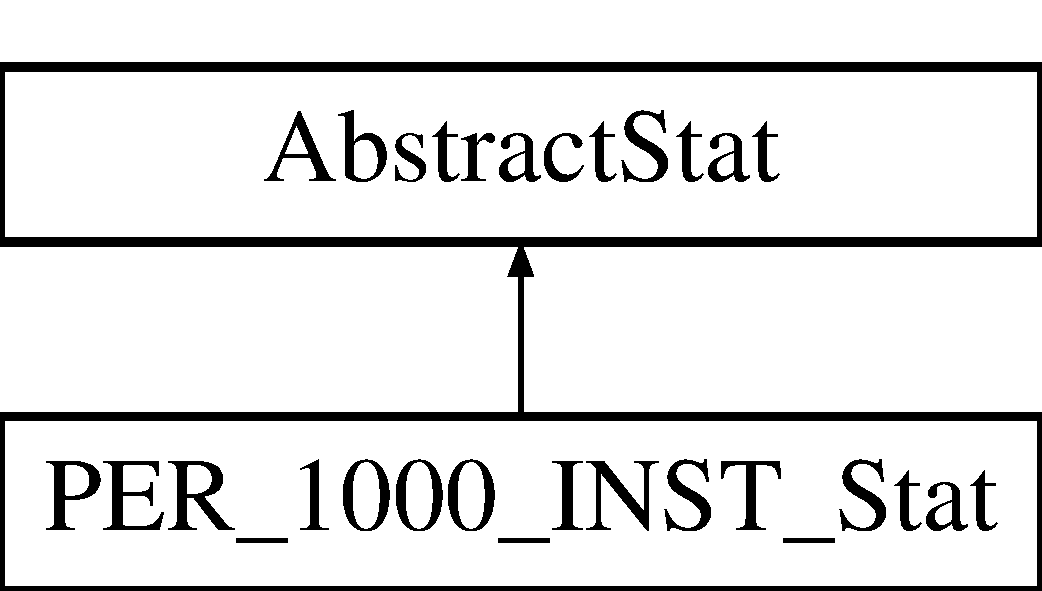
\includegraphics[height=2.000000cm]{classPER__1000__INST__Stat}
\end{center}
\end{figure}
\subsection*{Public Member Functions}
\begin{DoxyCompactItemize}
\item 
\hyperlink{classPER__1000__INST__Stat_ae928c5d8616cf8a0cd3e2721bb6a12a6}{PER\_\-1000\_\-INST\_\-Stat} (const string \&str, const string \&outputfilename, long ID)
\item 
virtual \hyperlink{classPER__1000__INST__Stat_ab68ba2b4b7f7808cd13dea3903ac85d1}{$\sim$PER\_\-1000\_\-INST\_\-Stat} ()
\item 
virtual \hyperlink{classAbstractStat}{AbstractStat} $\ast$ \hyperlink{classPER__1000__INST__Stat_aa91568b17fd503ba676dd22dfbc13e9a}{clone} (unsigned int coreID)
\item 
virtual void \hyperlink{classPER__1000__INST__Stat_adb9d735306e7c9a831c92662cfcb8824}{writeTo} (ofstream \&stream)
\end{DoxyCompactItemize}
\subsection*{Private Attributes}
\begin{DoxyCompactItemize}
\item 
float \hyperlink{classPER__1000__INST__Stat_a10fee97cef42d33172c4fc2f63bc7a71}{per\_\-1000\_\-inst\_\-value}
\end{DoxyCompactItemize}


\subsection{Detailed Description}
PER\_\-1000\_\-INST type stat. 

\subsection{Constructor \& Destructor Documentation}
\hypertarget{classPER__1000__INST__Stat_ae928c5d8616cf8a0cd3e2721bb6a12a6}{
\index{PER\_\-1000\_\-INST\_\-Stat@{PER\_\-1000\_\-INST\_\-Stat}!PER\_\-1000\_\-INST\_\-Stat@{PER\_\-1000\_\-INST\_\-Stat}}
\index{PER\_\-1000\_\-INST\_\-Stat@{PER\_\-1000\_\-INST\_\-Stat}!PER_1000_INST_Stat@{PER\_\-1000\_\-INST\_\-Stat}}
\subsubsection[{PER\_\-1000\_\-INST\_\-Stat}]{\setlength{\rightskip}{0pt plus 5cm}PER\_\-1000\_\-INST\_\-Stat::PER\_\-1000\_\-INST\_\-Stat (
\begin{DoxyParamCaption}
\item[{const string \&}]{ str, }
\item[{const string \&}]{ outputfilename, }
\item[{long}]{ ID}
\end{DoxyParamCaption}
)\hspace{0.3cm}{\ttfamily  \mbox{[}inline\mbox{]}}}}
\label{classPER__1000__INST__Stat_ae928c5d8616cf8a0cd3e2721bb6a12a6}
Constructor. \hypertarget{classPER__1000__INST__Stat_ab68ba2b4b7f7808cd13dea3903ac85d1}{
\index{PER\_\-1000\_\-INST\_\-Stat@{PER\_\-1000\_\-INST\_\-Stat}!$\sim$PER\_\-1000\_\-INST\_\-Stat@{$\sim$PER\_\-1000\_\-INST\_\-Stat}}
\index{$\sim$PER\_\-1000\_\-INST\_\-Stat@{$\sim$PER\_\-1000\_\-INST\_\-Stat}!PER_1000_INST_Stat@{PER\_\-1000\_\-INST\_\-Stat}}
\subsubsection[{$\sim$PER\_\-1000\_\-INST\_\-Stat}]{\setlength{\rightskip}{0pt plus 5cm}virtual PER\_\-1000\_\-INST\_\-Stat::$\sim$PER\_\-1000\_\-INST\_\-Stat (
\begin{DoxyParamCaption}
{}
\end{DoxyParamCaption}
)\hspace{0.3cm}{\ttfamily  \mbox{[}inline, virtual\mbox{]}}}}
\label{classPER__1000__INST__Stat_ab68ba2b4b7f7808cd13dea3903ac85d1}
Destructor. 

\subsection{Member Function Documentation}
\hypertarget{classPER__1000__INST__Stat_aa91568b17fd503ba676dd22dfbc13e9a}{
\index{PER\_\-1000\_\-INST\_\-Stat@{PER\_\-1000\_\-INST\_\-Stat}!clone@{clone}}
\index{clone@{clone}!PER_1000_INST_Stat@{PER\_\-1000\_\-INST\_\-Stat}}
\subsubsection[{clone}]{\setlength{\rightskip}{0pt plus 5cm}virtual {\bf AbstractStat}$\ast$ PER\_\-1000\_\-INST\_\-Stat::clone (
\begin{DoxyParamCaption}
\item[{unsigned int}]{ coreID}
\end{DoxyParamCaption}
)\hspace{0.3cm}{\ttfamily  \mbox{[}inline, virtual\mbox{]}}}}
\label{classPER__1000__INST__Stat_aa91568b17fd503ba676dd22dfbc13e9a}
Clone a stat. 

Implements \hyperlink{classAbstractStat_aed9a458491d92fb2cc3c458990d9fab1}{AbstractStat}.

\hypertarget{classPER__1000__INST__Stat_adb9d735306e7c9a831c92662cfcb8824}{
\index{PER\_\-1000\_\-INST\_\-Stat@{PER\_\-1000\_\-INST\_\-Stat}!writeTo@{writeTo}}
\index{writeTo@{writeTo}!PER_1000_INST_Stat@{PER\_\-1000\_\-INST\_\-Stat}}
\subsubsection[{writeTo}]{\setlength{\rightskip}{0pt plus 5cm}virtual void PER\_\-1000\_\-INST\_\-Stat::writeTo (
\begin{DoxyParamCaption}
\item[{ofstream \&}]{ stream}
\end{DoxyParamCaption}
)\hspace{0.3cm}{\ttfamily  \mbox{[}inline, virtual\mbox{]}}}}
\label{classPER__1000__INST__Stat_adb9d735306e7c9a831c92662cfcb8824}
Dump all stats to the file. 

Reimplemented from \hyperlink{classAbstractStat_aa4760247da47c70d7345de5d881f59cb}{AbstractStat}.



\subsection{Member Data Documentation}
\hypertarget{classPER__1000__INST__Stat_a10fee97cef42d33172c4fc2f63bc7a71}{
\index{PER\_\-1000\_\-INST\_\-Stat@{PER\_\-1000\_\-INST\_\-Stat}!per\_\-1000\_\-inst\_\-value@{per\_\-1000\_\-inst\_\-value}}
\index{per\_\-1000\_\-inst\_\-value@{per\_\-1000\_\-inst\_\-value}!PER_1000_INST_Stat@{PER\_\-1000\_\-INST\_\-Stat}}
\subsubsection[{per\_\-1000\_\-inst\_\-value}]{\setlength{\rightskip}{0pt plus 5cm}float {\bf PER\_\-1000\_\-INST\_\-Stat::per\_\-1000\_\-inst\_\-value}\hspace{0.3cm}{\ttfamily  \mbox{[}private\mbox{]}}}}
\label{classPER__1000__INST__Stat_a10fee97cef42d33172c4fc2f63bc7a71}
per 1000 instruction value 

The documentation for this class was generated from the following file:\begin{DoxyCompactItemize}
\item 
statistics.h\end{DoxyCompactItemize}

\hypertarget{classPER__1000__PRET__INST__Stat}{
\section{PER\_\-1000\_\-PRET\_\-INST\_\-Stat Class Reference}
\label{classPER__1000__PRET__INST__Stat}\index{PER\_\-1000\_\-PRET\_\-INST\_\-Stat@{PER\_\-1000\_\-PRET\_\-INST\_\-Stat}}
}


PER\_\-1000\_\-PRET\_\-INST type stat.  




{\ttfamily \#include $<$statistics.h$>$}

Inheritance diagram for PER\_\-1000\_\-PRET\_\-INST\_\-Stat:\begin{figure}[H]
\begin{center}
\leavevmode
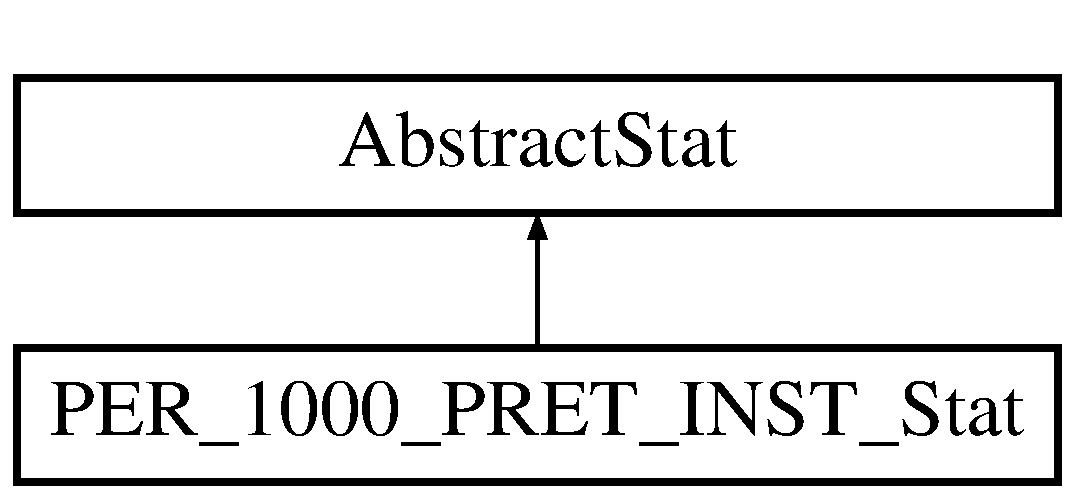
\includegraphics[height=2.000000cm]{classPER__1000__PRET__INST__Stat}
\end{center}
\end{figure}
\subsection*{Public Member Functions}
\begin{DoxyCompactItemize}
\item 
\hyperlink{classPER__1000__PRET__INST__Stat_a936a4cc95050a97b7281b7a2fa07207f}{PER\_\-1000\_\-PRET\_\-INST\_\-Stat} (const string \&str, const string \&outputfilename, long ID)
\item 
virtual \hyperlink{classPER__1000__PRET__INST__Stat_a9726ed3943763009bcc37f8dab33411d}{$\sim$PER\_\-1000\_\-PRET\_\-INST\_\-Stat} ()
\item 
virtual \hyperlink{classAbstractStat}{AbstractStat} $\ast$ \hyperlink{classPER__1000__PRET__INST__Stat_a2aca938ef3f2acc92c46e3386680e5aa}{clone} (unsigned int coreID)
\item 
virtual void \hyperlink{classPER__1000__PRET__INST__Stat_aa353396e1c813cd55b6023de87abd807}{writeTo} (ofstream \&stream)
\end{DoxyCompactItemize}
\subsection*{Private Attributes}
\begin{DoxyCompactItemize}
\item 
float \hyperlink{classPER__1000__PRET__INST__Stat_a00fced31ff12b4b45b9d9e43aae01a60}{per\_\-1000\_\-pret\_\-inst\_\-value}
\end{DoxyCompactItemize}


\subsection{Detailed Description}
PER\_\-1000\_\-PRET\_\-INST type stat. 

\subsection{Constructor \& Destructor Documentation}
\hypertarget{classPER__1000__PRET__INST__Stat_a936a4cc95050a97b7281b7a2fa07207f}{
\index{PER\_\-1000\_\-PRET\_\-INST\_\-Stat@{PER\_\-1000\_\-PRET\_\-INST\_\-Stat}!PER\_\-1000\_\-PRET\_\-INST\_\-Stat@{PER\_\-1000\_\-PRET\_\-INST\_\-Stat}}
\index{PER\_\-1000\_\-PRET\_\-INST\_\-Stat@{PER\_\-1000\_\-PRET\_\-INST\_\-Stat}!PER_1000_PRET_INST_Stat@{PER\_\-1000\_\-PRET\_\-INST\_\-Stat}}
\subsubsection[{PER\_\-1000\_\-PRET\_\-INST\_\-Stat}]{\setlength{\rightskip}{0pt plus 5cm}PER\_\-1000\_\-PRET\_\-INST\_\-Stat::PER\_\-1000\_\-PRET\_\-INST\_\-Stat (
\begin{DoxyParamCaption}
\item[{const string \&}]{ str, }
\item[{const string \&}]{ outputfilename, }
\item[{long}]{ ID}
\end{DoxyParamCaption}
)\hspace{0.3cm}{\ttfamily  \mbox{[}inline\mbox{]}}}}
\label{classPER__1000__PRET__INST__Stat_a936a4cc95050a97b7281b7a2fa07207f}
Constructor. \hypertarget{classPER__1000__PRET__INST__Stat_a9726ed3943763009bcc37f8dab33411d}{
\index{PER\_\-1000\_\-PRET\_\-INST\_\-Stat@{PER\_\-1000\_\-PRET\_\-INST\_\-Stat}!$\sim$PER\_\-1000\_\-PRET\_\-INST\_\-Stat@{$\sim$PER\_\-1000\_\-PRET\_\-INST\_\-Stat}}
\index{$\sim$PER\_\-1000\_\-PRET\_\-INST\_\-Stat@{$\sim$PER\_\-1000\_\-PRET\_\-INST\_\-Stat}!PER_1000_PRET_INST_Stat@{PER\_\-1000\_\-PRET\_\-INST\_\-Stat}}
\subsubsection[{$\sim$PER\_\-1000\_\-PRET\_\-INST\_\-Stat}]{\setlength{\rightskip}{0pt plus 5cm}virtual PER\_\-1000\_\-PRET\_\-INST\_\-Stat::$\sim$PER\_\-1000\_\-PRET\_\-INST\_\-Stat (
\begin{DoxyParamCaption}
{}
\end{DoxyParamCaption}
)\hspace{0.3cm}{\ttfamily  \mbox{[}inline, virtual\mbox{]}}}}
\label{classPER__1000__PRET__INST__Stat_a9726ed3943763009bcc37f8dab33411d}
Destructor. 

\subsection{Member Function Documentation}
\hypertarget{classPER__1000__PRET__INST__Stat_a2aca938ef3f2acc92c46e3386680e5aa}{
\index{PER\_\-1000\_\-PRET\_\-INST\_\-Stat@{PER\_\-1000\_\-PRET\_\-INST\_\-Stat}!clone@{clone}}
\index{clone@{clone}!PER_1000_PRET_INST_Stat@{PER\_\-1000\_\-PRET\_\-INST\_\-Stat}}
\subsubsection[{clone}]{\setlength{\rightskip}{0pt plus 5cm}virtual {\bf AbstractStat}$\ast$ PER\_\-1000\_\-PRET\_\-INST\_\-Stat::clone (
\begin{DoxyParamCaption}
\item[{unsigned int}]{ coreID}
\end{DoxyParamCaption}
)\hspace{0.3cm}{\ttfamily  \mbox{[}inline, virtual\mbox{]}}}}
\label{classPER__1000__PRET__INST__Stat_a2aca938ef3f2acc92c46e3386680e5aa}
Clone a stat. 

Implements \hyperlink{classAbstractStat_aed9a458491d92fb2cc3c458990d9fab1}{AbstractStat}.

\hypertarget{classPER__1000__PRET__INST__Stat_aa353396e1c813cd55b6023de87abd807}{
\index{PER\_\-1000\_\-PRET\_\-INST\_\-Stat@{PER\_\-1000\_\-PRET\_\-INST\_\-Stat}!writeTo@{writeTo}}
\index{writeTo@{writeTo}!PER_1000_PRET_INST_Stat@{PER\_\-1000\_\-PRET\_\-INST\_\-Stat}}
\subsubsection[{writeTo}]{\setlength{\rightskip}{0pt plus 5cm}virtual void PER\_\-1000\_\-PRET\_\-INST\_\-Stat::writeTo (
\begin{DoxyParamCaption}
\item[{ofstream \&}]{ stream}
\end{DoxyParamCaption}
)\hspace{0.3cm}{\ttfamily  \mbox{[}inline, virtual\mbox{]}}}}
\label{classPER__1000__PRET__INST__Stat_aa353396e1c813cd55b6023de87abd807}
Dump stats to the file. 

Reimplemented from \hyperlink{classAbstractStat_aa4760247da47c70d7345de5d881f59cb}{AbstractStat}.



\subsection{Member Data Documentation}
\hypertarget{classPER__1000__PRET__INST__Stat_a00fced31ff12b4b45b9d9e43aae01a60}{
\index{PER\_\-1000\_\-PRET\_\-INST\_\-Stat@{PER\_\-1000\_\-PRET\_\-INST\_\-Stat}!per\_\-1000\_\-pret\_\-inst\_\-value@{per\_\-1000\_\-pret\_\-inst\_\-value}}
\index{per\_\-1000\_\-pret\_\-inst\_\-value@{per\_\-1000\_\-pret\_\-inst\_\-value}!PER_1000_PRET_INST_Stat@{PER\_\-1000\_\-PRET\_\-INST\_\-Stat}}
\subsubsection[{per\_\-1000\_\-pret\_\-inst\_\-value}]{\setlength{\rightskip}{0pt plus 5cm}float {\bf PER\_\-1000\_\-PRET\_\-INST\_\-Stat::per\_\-1000\_\-pret\_\-inst\_\-value}\hspace{0.3cm}{\ttfamily  \mbox{[}private\mbox{]}}}}
\label{classPER__1000__PRET__INST__Stat_a00fced31ff12b4b45b9d9e43aae01a60}
stat value 

The documentation for this class was generated from the following file:\begin{DoxyCompactItemize}
\item 
statistics.h\end{DoxyCompactItemize}

\hypertarget{classPER__CYCLE__Stat}{
\section{PER\_\-CYCLE\_\-Stat Class Reference}
\label{classPER__CYCLE__Stat}\index{PER\_\-CYCLE\_\-Stat@{PER\_\-CYCLE\_\-Stat}}
}


PER\_\-CYCLE stat.  




{\ttfamily \#include $<$statistics.h$>$}

Inheritance diagram for PER\_\-CYCLE\_\-Stat:\begin{figure}[H]
\begin{center}
\leavevmode
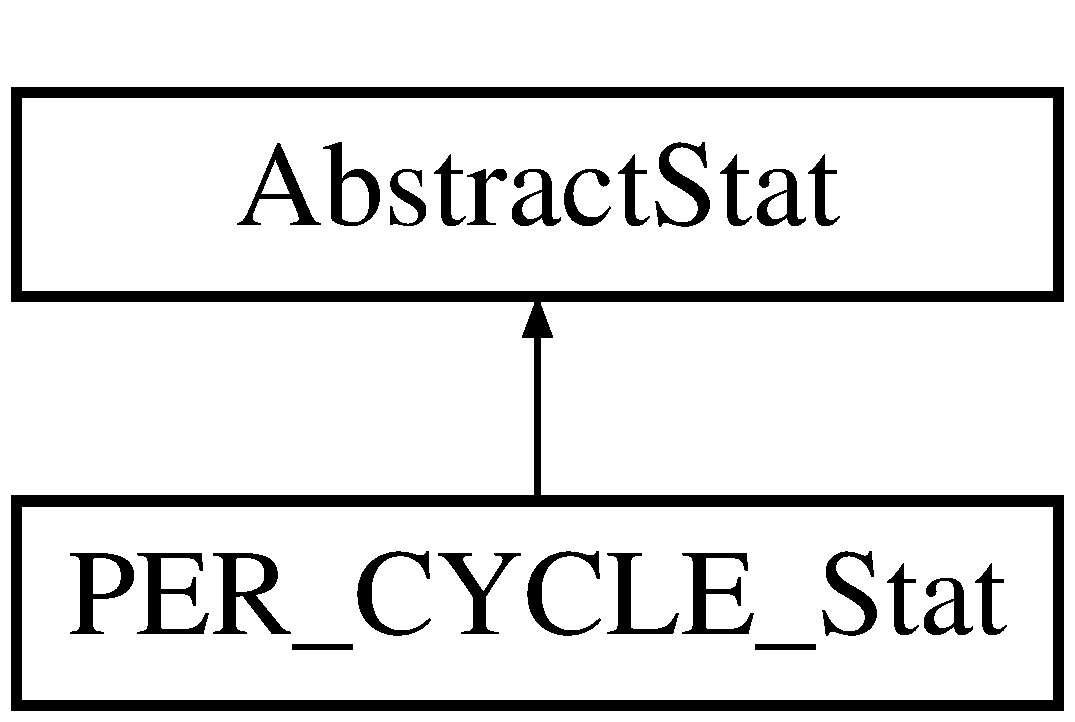
\includegraphics[height=2.000000cm]{classPER__CYCLE__Stat}
\end{center}
\end{figure}
\subsection*{Public Member Functions}
\begin{DoxyCompactItemize}
\item 
\hyperlink{classPER__CYCLE__Stat_aeca09801bc358cd3f0e6efd6e26f667a}{PER\_\-CYCLE\_\-Stat} (const string \&str, const string \&outputfilename, long ID)
\item 
virtual \hyperlink{classPER__CYCLE__Stat_a6b6ad6f5d210941b1893f2a0cb8f1b4c}{$\sim$PER\_\-CYCLE\_\-Stat} ()
\item 
virtual \hyperlink{classAbstractStat}{AbstractStat} $\ast$ \hyperlink{classPER__CYCLE__Stat_ae97b00337c422362a6a234b854141bdc}{clone} (unsigned int coreID)
\item 
virtual void \hyperlink{classPER__CYCLE__Stat_afbaf94b274ded7040fe3592a44cc5769}{writeTo} (ofstream \&stream)
\end{DoxyCompactItemize}
\subsection*{Private Attributes}
\begin{DoxyCompactItemize}
\item 
float \hyperlink{classPER__CYCLE__Stat_a01dce57aa26a221ac719276fafa58396}{per\_\-cycle}
\end{DoxyCompactItemize}


\subsection{Detailed Description}
PER\_\-CYCLE stat. 

\subsection{Constructor \& Destructor Documentation}
\hypertarget{classPER__CYCLE__Stat_aeca09801bc358cd3f0e6efd6e26f667a}{
\index{PER\_\-CYCLE\_\-Stat@{PER\_\-CYCLE\_\-Stat}!PER\_\-CYCLE\_\-Stat@{PER\_\-CYCLE\_\-Stat}}
\index{PER\_\-CYCLE\_\-Stat@{PER\_\-CYCLE\_\-Stat}!PER_CYCLE_Stat@{PER\_\-CYCLE\_\-Stat}}
\subsubsection[{PER\_\-CYCLE\_\-Stat}]{\setlength{\rightskip}{0pt plus 5cm}PER\_\-CYCLE\_\-Stat::PER\_\-CYCLE\_\-Stat (
\begin{DoxyParamCaption}
\item[{const string \&}]{ str, }
\item[{const string \&}]{ outputfilename, }
\item[{long}]{ ID}
\end{DoxyParamCaption}
)\hspace{0.3cm}{\ttfamily  \mbox{[}inline\mbox{]}}}}
\label{classPER__CYCLE__Stat_aeca09801bc358cd3f0e6efd6e26f667a}
Constructor. \hypertarget{classPER__CYCLE__Stat_a6b6ad6f5d210941b1893f2a0cb8f1b4c}{
\index{PER\_\-CYCLE\_\-Stat@{PER\_\-CYCLE\_\-Stat}!$\sim$PER\_\-CYCLE\_\-Stat@{$\sim$PER\_\-CYCLE\_\-Stat}}
\index{$\sim$PER\_\-CYCLE\_\-Stat@{$\sim$PER\_\-CYCLE\_\-Stat}!PER_CYCLE_Stat@{PER\_\-CYCLE\_\-Stat}}
\subsubsection[{$\sim$PER\_\-CYCLE\_\-Stat}]{\setlength{\rightskip}{0pt plus 5cm}virtual PER\_\-CYCLE\_\-Stat::$\sim$PER\_\-CYCLE\_\-Stat (
\begin{DoxyParamCaption}
{}
\end{DoxyParamCaption}
)\hspace{0.3cm}{\ttfamily  \mbox{[}inline, virtual\mbox{]}}}}
\label{classPER__CYCLE__Stat_a6b6ad6f5d210941b1893f2a0cb8f1b4c}
Destructor. 

\subsection{Member Function Documentation}
\hypertarget{classPER__CYCLE__Stat_ae97b00337c422362a6a234b854141bdc}{
\index{PER\_\-CYCLE\_\-Stat@{PER\_\-CYCLE\_\-Stat}!clone@{clone}}
\index{clone@{clone}!PER_CYCLE_Stat@{PER\_\-CYCLE\_\-Stat}}
\subsubsection[{clone}]{\setlength{\rightskip}{0pt plus 5cm}virtual {\bf AbstractStat}$\ast$ PER\_\-CYCLE\_\-Stat::clone (
\begin{DoxyParamCaption}
\item[{unsigned int}]{ coreID}
\end{DoxyParamCaption}
)\hspace{0.3cm}{\ttfamily  \mbox{[}inline, virtual\mbox{]}}}}
\label{classPER__CYCLE__Stat_ae97b00337c422362a6a234b854141bdc}
Clone a stat. 

Implements \hyperlink{classAbstractStat_aed9a458491d92fb2cc3c458990d9fab1}{AbstractStat}.

\hypertarget{classPER__CYCLE__Stat_afbaf94b274ded7040fe3592a44cc5769}{
\index{PER\_\-CYCLE\_\-Stat@{PER\_\-CYCLE\_\-Stat}!writeTo@{writeTo}}
\index{writeTo@{writeTo}!PER_CYCLE_Stat@{PER\_\-CYCLE\_\-Stat}}
\subsubsection[{writeTo}]{\setlength{\rightskip}{0pt plus 5cm}virtual void PER\_\-CYCLE\_\-Stat::writeTo (
\begin{DoxyParamCaption}
\item[{ofstream \&}]{ stream}
\end{DoxyParamCaption}
)\hspace{0.3cm}{\ttfamily  \mbox{[}inline, virtual\mbox{]}}}}
\label{classPER__CYCLE__Stat_afbaf94b274ded7040fe3592a44cc5769}
Dump out all stats to the file. 

Reimplemented from \hyperlink{classAbstractStat_aa4760247da47c70d7345de5d881f59cb}{AbstractStat}.



\subsection{Member Data Documentation}
\hypertarget{classPER__CYCLE__Stat_a01dce57aa26a221ac719276fafa58396}{
\index{PER\_\-CYCLE\_\-Stat@{PER\_\-CYCLE\_\-Stat}!per\_\-cycle@{per\_\-cycle}}
\index{per\_\-cycle@{per\_\-cycle}!PER_CYCLE_Stat@{PER\_\-CYCLE\_\-Stat}}
\subsubsection[{per\_\-cycle}]{\setlength{\rightskip}{0pt plus 5cm}float {\bf PER\_\-CYCLE\_\-Stat::per\_\-cycle}\hspace{0.3cm}{\ttfamily  \mbox{[}private\mbox{]}}}}
\label{classPER__CYCLE__Stat_a01dce57aa26a221ac719276fafa58396}
stat value 

The documentation for this class was generated from the following file:\begin{DoxyCompactItemize}
\item 
statistics.h\end{DoxyCompactItemize}

\hypertarget{classPER__INST__Stat}{
\section{PER\_\-INST\_\-Stat Class Reference}
\label{classPER__INST__Stat}\index{PER\_\-INST\_\-Stat@{PER\_\-INST\_\-Stat}}
}


PER\_\-INST type stat.  




{\ttfamily \#include $<$statistics.h$>$}

Inheritance diagram for PER\_\-INST\_\-Stat:\begin{figure}[H]
\begin{center}
\leavevmode
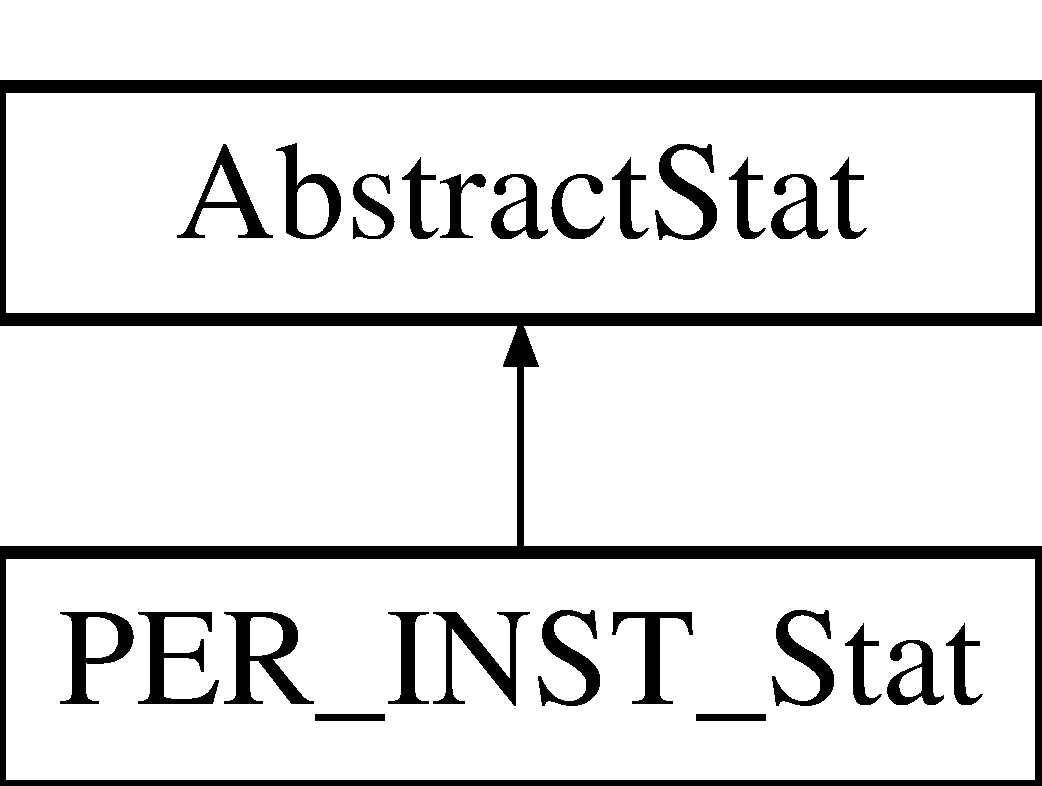
\includegraphics[height=2.000000cm]{classPER__INST__Stat}
\end{center}
\end{figure}
\subsection*{Public Member Functions}
\begin{DoxyCompactItemize}
\item 
\hyperlink{classPER__INST__Stat_aabfaf17917f7d000cca7a88baba533a4}{PER\_\-INST\_\-Stat} (const string \&str, const string \&outputfilename, long ID)
\item 
virtual \hyperlink{classPER__INST__Stat_a6f3a65cdcd74729016d755bfed571a6c}{$\sim$PER\_\-INST\_\-Stat} ()
\item 
virtual \hyperlink{classAbstractStat}{AbstractStat} $\ast$ \hyperlink{classPER__INST__Stat_a46a249720fb40d3ddef0c2f39c241c03}{clone} (unsigned int coreID)
\item 
virtual void \hyperlink{classPER__INST__Stat_ad7ffab56cc4bbd33c3332de3863e9b54}{writeTo} (ofstream \&stream)
\end{DoxyCompactItemize}
\subsection*{Private Attributes}
\begin{DoxyCompactItemize}
\item 
float \hyperlink{classPER__INST__Stat_a1678ba031f3e53cdca033aac3e352925}{per\_\-inst\_\-value}
\end{DoxyCompactItemize}


\subsection{Detailed Description}
PER\_\-INST type stat. 

\subsection{Constructor \& Destructor Documentation}
\hypertarget{classPER__INST__Stat_aabfaf17917f7d000cca7a88baba533a4}{
\index{PER\_\-INST\_\-Stat@{PER\_\-INST\_\-Stat}!PER\_\-INST\_\-Stat@{PER\_\-INST\_\-Stat}}
\index{PER\_\-INST\_\-Stat@{PER\_\-INST\_\-Stat}!PER_INST_Stat@{PER\_\-INST\_\-Stat}}
\subsubsection[{PER\_\-INST\_\-Stat}]{\setlength{\rightskip}{0pt plus 5cm}PER\_\-INST\_\-Stat::PER\_\-INST\_\-Stat (
\begin{DoxyParamCaption}
\item[{const string \&}]{ str, }
\item[{const string \&}]{ outputfilename, }
\item[{long}]{ ID}
\end{DoxyParamCaption}
)\hspace{0.3cm}{\ttfamily  \mbox{[}inline\mbox{]}}}}
\label{classPER__INST__Stat_aabfaf17917f7d000cca7a88baba533a4}
Constructor \hypertarget{classPER__INST__Stat_a6f3a65cdcd74729016d755bfed571a6c}{
\index{PER\_\-INST\_\-Stat@{PER\_\-INST\_\-Stat}!$\sim$PER\_\-INST\_\-Stat@{$\sim$PER\_\-INST\_\-Stat}}
\index{$\sim$PER\_\-INST\_\-Stat@{$\sim$PER\_\-INST\_\-Stat}!PER_INST_Stat@{PER\_\-INST\_\-Stat}}
\subsubsection[{$\sim$PER\_\-INST\_\-Stat}]{\setlength{\rightskip}{0pt plus 5cm}virtual PER\_\-INST\_\-Stat::$\sim$PER\_\-INST\_\-Stat (
\begin{DoxyParamCaption}
{}
\end{DoxyParamCaption}
)\hspace{0.3cm}{\ttfamily  \mbox{[}inline, virtual\mbox{]}}}}
\label{classPER__INST__Stat_a6f3a65cdcd74729016d755bfed571a6c}
Destructor. 

\subsection{Member Function Documentation}
\hypertarget{classPER__INST__Stat_a46a249720fb40d3ddef0c2f39c241c03}{
\index{PER\_\-INST\_\-Stat@{PER\_\-INST\_\-Stat}!clone@{clone}}
\index{clone@{clone}!PER_INST_Stat@{PER\_\-INST\_\-Stat}}
\subsubsection[{clone}]{\setlength{\rightskip}{0pt plus 5cm}virtual {\bf AbstractStat}$\ast$ PER\_\-INST\_\-Stat::clone (
\begin{DoxyParamCaption}
\item[{unsigned int}]{ coreID}
\end{DoxyParamCaption}
)\hspace{0.3cm}{\ttfamily  \mbox{[}inline, virtual\mbox{]}}}}
\label{classPER__INST__Stat_a46a249720fb40d3ddef0c2f39c241c03}
Clone a stat. 

Implements \hyperlink{classAbstractStat_aed9a458491d92fb2cc3c458990d9fab1}{AbstractStat}.

\hypertarget{classPER__INST__Stat_ad7ffab56cc4bbd33c3332de3863e9b54}{
\index{PER\_\-INST\_\-Stat@{PER\_\-INST\_\-Stat}!writeTo@{writeTo}}
\index{writeTo@{writeTo}!PER_INST_Stat@{PER\_\-INST\_\-Stat}}
\subsubsection[{writeTo}]{\setlength{\rightskip}{0pt plus 5cm}virtual void PER\_\-INST\_\-Stat::writeTo (
\begin{DoxyParamCaption}
\item[{ofstream \&}]{ stream}
\end{DoxyParamCaption}
)\hspace{0.3cm}{\ttfamily  \mbox{[}inline, virtual\mbox{]}}}}
\label{classPER__INST__Stat_ad7ffab56cc4bbd33c3332de3863e9b54}
Dump out all stats to the file. 

Reimplemented from \hyperlink{classAbstractStat_aa4760247da47c70d7345de5d881f59cb}{AbstractStat}.



\subsection{Member Data Documentation}
\hypertarget{classPER__INST__Stat_a1678ba031f3e53cdca033aac3e352925}{
\index{PER\_\-INST\_\-Stat@{PER\_\-INST\_\-Stat}!per\_\-inst\_\-value@{per\_\-inst\_\-value}}
\index{per\_\-inst\_\-value@{per\_\-inst\_\-value}!PER_INST_Stat@{PER\_\-INST\_\-Stat}}
\subsubsection[{per\_\-inst\_\-value}]{\setlength{\rightskip}{0pt plus 5cm}float {\bf PER\_\-INST\_\-Stat::per\_\-inst\_\-value}\hspace{0.3cm}{\ttfamily  \mbox{[}private\mbox{]}}}}
\label{classPER__INST__Stat_a1678ba031f3e53cdca033aac3e352925}
stat value 

The documentation for this class was generated from the following file:\begin{DoxyCompactItemize}
\item 
statistics.h\end{DoxyCompactItemize}

\hypertarget{classPERCENT__Stat}{
\section{PERCENT\_\-Stat Class Reference}
\label{classPERCENT__Stat}\index{PERCENT\_\-Stat@{PERCENT\_\-Stat}}
}


PERCENT type stat.  




{\ttfamily \#include $<$statistics.h$>$}

Inheritance diagram for PERCENT\_\-Stat:\begin{figure}[H]
\begin{center}
\leavevmode
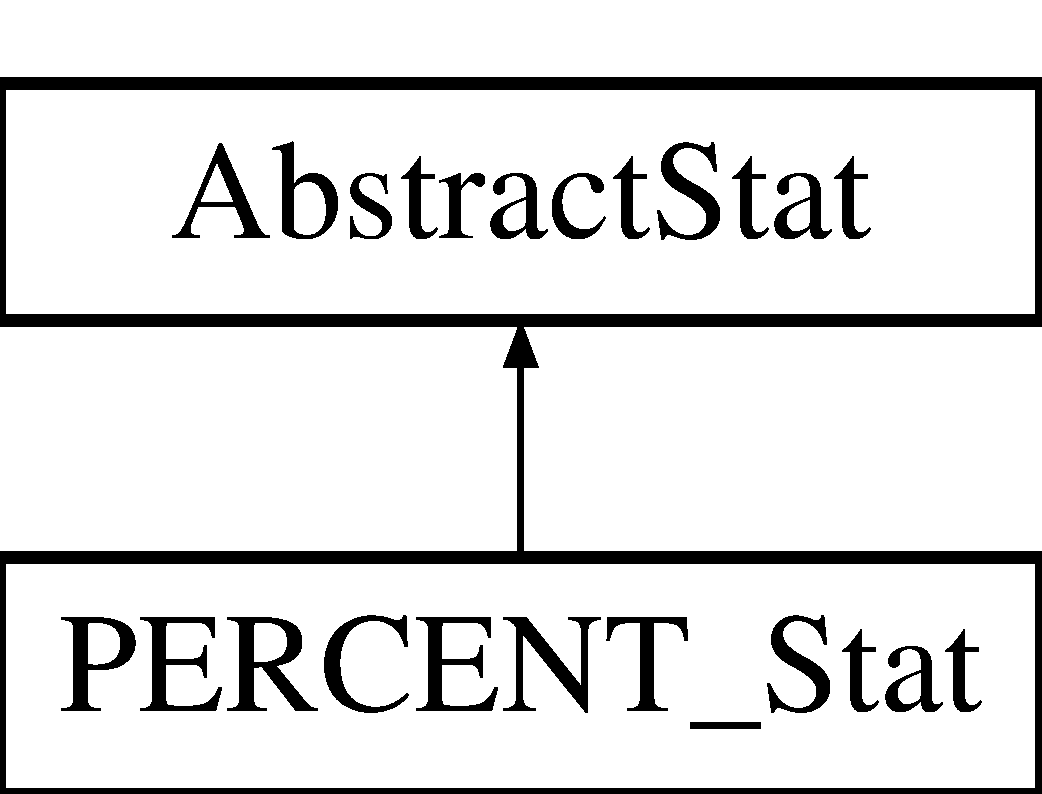
\includegraphics[height=2.000000cm]{classPERCENT__Stat}
\end{center}
\end{figure}
\subsection*{Public Member Functions}
\begin{DoxyCompactItemize}
\item 
\hyperlink{classPERCENT__Stat_a75de30141ea55a2219a4d9fcb6b9097b}{PERCENT\_\-Stat} (const string \&str, const string \&outputfilename, long ID, long denominatorID, \hyperlink{classProcessorStatistics}{ProcessorStatistics} $\ast$procStat)
\item 
virtual \hyperlink{classPERCENT__Stat_a0b1d53d550e454d48d0103c321159d9d}{$\sim$PERCENT\_\-Stat} ()
\item 
virtual \hyperlink{classAbstractStat}{AbstractStat} $\ast$ \hyperlink{classPERCENT__Stat_addd937bd0a1e3649ee2fb6e336ef5955}{clone} (unsigned int coreID)
\item 
virtual void \hyperlink{classPERCENT__Stat_a927dba3cbaf53d4bc05de92f682f9c80}{writeTo} (ofstream \&stream)
\end{DoxyCompactItemize}
\subsection*{Private Attributes}
\begin{DoxyCompactItemize}
\item 
long \hyperlink{classPERCENT__Stat_a0079cc34c77679a78843bf6788e7e4b3}{m\_\-denominatorID}
\item 
float \hyperlink{classPERCENT__Stat_acceb28a0ccaf48ba31b576c0f88b1303}{ratio}
\item 
float \hyperlink{classPERCENT__Stat_a51c6f05b501728724644b0a831abd1eb}{percent}
\item 
\hyperlink{classProcessorStatistics}{ProcessorStatistics} $\ast$ \hyperlink{classPERCENT__Stat_aaa7e252b1f03c04d1f16b78f360cc601}{m\_\-ProcStat}
\end{DoxyCompactItemize}


\subsection{Detailed Description}
PERCENT type stat. 

\subsection{Constructor \& Destructor Documentation}
\hypertarget{classPERCENT__Stat_a75de30141ea55a2219a4d9fcb6b9097b}{
\index{PERCENT\_\-Stat@{PERCENT\_\-Stat}!PERCENT\_\-Stat@{PERCENT\_\-Stat}}
\index{PERCENT\_\-Stat@{PERCENT\_\-Stat}!PERCENT_Stat@{PERCENT\_\-Stat}}
\subsubsection[{PERCENT\_\-Stat}]{\setlength{\rightskip}{0pt plus 5cm}PERCENT\_\-Stat::PERCENT\_\-Stat (
\begin{DoxyParamCaption}
\item[{const string \&}]{ str, }
\item[{const string \&}]{ outputfilename, }
\item[{long}]{ ID, }
\item[{long}]{ denominatorID, }
\item[{{\bf ProcessorStatistics} $\ast$}]{ procStat}
\end{DoxyParamCaption}
)\hspace{0.3cm}{\ttfamily  \mbox{[}inline\mbox{]}}}}
\label{classPERCENT__Stat_a75de30141ea55a2219a4d9fcb6b9097b}
Constructor. \hypertarget{classPERCENT__Stat_a0b1d53d550e454d48d0103c321159d9d}{
\index{PERCENT\_\-Stat@{PERCENT\_\-Stat}!$\sim$PERCENT\_\-Stat@{$\sim$PERCENT\_\-Stat}}
\index{$\sim$PERCENT\_\-Stat@{$\sim$PERCENT\_\-Stat}!PERCENT_Stat@{PERCENT\_\-Stat}}
\subsubsection[{$\sim$PERCENT\_\-Stat}]{\setlength{\rightskip}{0pt plus 5cm}virtual PERCENT\_\-Stat::$\sim$PERCENT\_\-Stat (
\begin{DoxyParamCaption}
{}
\end{DoxyParamCaption}
)\hspace{0.3cm}{\ttfamily  \mbox{[}inline, virtual\mbox{]}}}}
\label{classPERCENT__Stat_a0b1d53d550e454d48d0103c321159d9d}
Destructor 

\subsection{Member Function Documentation}
\hypertarget{classPERCENT__Stat_addd937bd0a1e3649ee2fb6e336ef5955}{
\index{PERCENT\_\-Stat@{PERCENT\_\-Stat}!clone@{clone}}
\index{clone@{clone}!PERCENT_Stat@{PERCENT\_\-Stat}}
\subsubsection[{clone}]{\setlength{\rightskip}{0pt plus 5cm}virtual {\bf AbstractStat}$\ast$ PERCENT\_\-Stat::clone (
\begin{DoxyParamCaption}
\item[{unsigned int}]{ coreID}
\end{DoxyParamCaption}
)\hspace{0.3cm}{\ttfamily  \mbox{[}inline, virtual\mbox{]}}}}
\label{classPERCENT__Stat_addd937bd0a1e3649ee2fb6e336ef5955}
Clone a stat. 

Implements \hyperlink{classAbstractStat_aed9a458491d92fb2cc3c458990d9fab1}{AbstractStat}.

\hypertarget{classPERCENT__Stat_a927dba3cbaf53d4bc05de92f682f9c80}{
\index{PERCENT\_\-Stat@{PERCENT\_\-Stat}!writeTo@{writeTo}}
\index{writeTo@{writeTo}!PERCENT_Stat@{PERCENT\_\-Stat}}
\subsubsection[{writeTo}]{\setlength{\rightskip}{0pt plus 5cm}virtual void PERCENT\_\-Stat::writeTo (
\begin{DoxyParamCaption}
\item[{ofstream \&}]{ stream}
\end{DoxyParamCaption}
)\hspace{0.3cm}{\ttfamily  \mbox{[}inline, virtual\mbox{]}}}}
\label{classPERCENT__Stat_a927dba3cbaf53d4bc05de92f682f9c80}
Dump out all stats to the file. 

Reimplemented from \hyperlink{classAbstractStat_aa4760247da47c70d7345de5d881f59cb}{AbstractStat}.



\subsection{Member Data Documentation}
\hypertarget{classPERCENT__Stat_a0079cc34c77679a78843bf6788e7e4b3}{
\index{PERCENT\_\-Stat@{PERCENT\_\-Stat}!m\_\-denominatorID@{m\_\-denominatorID}}
\index{m\_\-denominatorID@{m\_\-denominatorID}!PERCENT_Stat@{PERCENT\_\-Stat}}
\subsubsection[{m\_\-denominatorID}]{\setlength{\rightskip}{0pt plus 5cm}long {\bf PERCENT\_\-Stat::m\_\-denominatorID}\hspace{0.3cm}{\ttfamily  \mbox{[}private\mbox{]}}}}
\label{classPERCENT__Stat_a0079cc34c77679a78843bf6788e7e4b3}
stat id \hypertarget{classPERCENT__Stat_aaa7e252b1f03c04d1f16b78f360cc601}{
\index{PERCENT\_\-Stat@{PERCENT\_\-Stat}!m\_\-ProcStat@{m\_\-ProcStat}}
\index{m\_\-ProcStat@{m\_\-ProcStat}!PERCENT_Stat@{PERCENT\_\-Stat}}
\subsubsection[{m\_\-ProcStat}]{\setlength{\rightskip}{0pt plus 5cm}{\bf ProcessorStatistics}$\ast$ {\bf PERCENT\_\-Stat::m\_\-ProcStat}\hspace{0.3cm}{\ttfamily  \mbox{[}private\mbox{]}}}}
\label{classPERCENT__Stat_aaa7e252b1f03c04d1f16b78f360cc601}
reference to simulation-\/scoped processor stats \hypertarget{classPERCENT__Stat_a51c6f05b501728724644b0a831abd1eb}{
\index{PERCENT\_\-Stat@{PERCENT\_\-Stat}!percent@{percent}}
\index{percent@{percent}!PERCENT_Stat@{PERCENT\_\-Stat}}
\subsubsection[{percent}]{\setlength{\rightskip}{0pt plus 5cm}float {\bf PERCENT\_\-Stat::percent}\hspace{0.3cm}{\ttfamily  \mbox{[}private\mbox{]}}}}
\label{classPERCENT__Stat_a51c6f05b501728724644b0a831abd1eb}
percent \hypertarget{classPERCENT__Stat_acceb28a0ccaf48ba31b576c0f88b1303}{
\index{PERCENT\_\-Stat@{PERCENT\_\-Stat}!ratio@{ratio}}
\index{ratio@{ratio}!PERCENT_Stat@{PERCENT\_\-Stat}}
\subsubsection[{ratio}]{\setlength{\rightskip}{0pt plus 5cm}float {\bf PERCENT\_\-Stat::ratio}\hspace{0.3cm}{\ttfamily  \mbox{[}private\mbox{]}}}}
\label{classPERCENT__Stat_acceb28a0ccaf48ba31b576c0f88b1303}
ratio 

The documentation for this class was generated from the following file:\begin{DoxyCompactItemize}
\item 
statistics.h\end{DoxyCompactItemize}

\hypertarget{classpool__c}{
\section{pool\_\-c$<$ T $>$ Class Template Reference}
\label{classpool__c}\index{pool\_\-c@{pool\_\-c}}
}


pool class  




{\ttfamily \#include $<$utils.h$>$}

\subsection*{Public Member Functions}
\begin{DoxyCompactItemize}
\item 
\hyperlink{classpool__c_ae046e396e7ac770f08794f37af913baf}{pool\_\-c} ()
\item 
\hyperlink{classpool__c_a27cca5145487122c44e63312edb95e40}{pool\_\-c} (int pool\_\-expand\_\-unit, string name)
\item 
\hyperlink{classpool__c_a398d3ecde03402f50fc02a0b04ae18e4}{$\sim$pool\_\-c} ()
\item 
T $\ast$ \hyperlink{classpool__c_a71f6e723ae8fef36d79ad5635edd2411}{acquire\_\-entry} (void)
\item 
T $\ast$ \hyperlink{classpool__c_abc21d62ac4f9d941fbe211d0decd5f7e}{acquire\_\-entry} (\hyperlink{classmacsim__c}{macsim\_\-c} $\ast$m\_\-simBase)
\item 
void \hyperlink{classpool__c_ac407b5245c7977b5baa5087ecbb395f2}{release\_\-entry} (T $\ast$entry)
\item 
void \hyperlink{classpool__c_a5bf9f2ef7e204b5f42feebf5394d00b7}{expand\_\-pool} (void)
\item 
void \hyperlink{classpool__c_a30c82c339cab1f22f427dc4189ebea66}{expand\_\-pool} (\hyperlink{classmacsim__c}{macsim\_\-c} $\ast$m\_\-simBase)
\item 
\hypertarget{classpool__c_a0589bbfc3b435c81cf4cd789a5fef668}{
int {\bfseries size} (void)}
\label{classpool__c_a0589bbfc3b435c81cf4cd789a5fef668}

\end{DoxyCompactItemize}
\subsection*{Private Attributes}
\begin{DoxyCompactItemize}
\item 
list$<$ T $\ast$ $>$ $\ast$ \hyperlink{classpool__c_ad882da850ef2313b4f2fb6c34ef3d760}{m\_\-pool}
\item 
int \hyperlink{classpool__c_aa20a955bf65ee7898e1028a76384c7bc}{m\_\-poolsize}
\item 
int \hyperlink{classpool__c_a439d24816449390c4b7ff8b9cac84faf}{m\_\-poolexpand\_\-unit}
\item 
string \hyperlink{classpool__c_a38ccabc9cf0fe92037e915485f02bf98}{m\_\-name}
\end{DoxyCompactItemize}


\subsection{Detailed Description}
\subsubsection*{template$<$class T$>$ class pool\_\-c$<$ T $>$}

pool class 

\subsection{Constructor \& Destructor Documentation}
\hypertarget{classpool__c_ae046e396e7ac770f08794f37af913baf}{
\index{pool\_\-c@{pool\_\-c}!pool\_\-c@{pool\_\-c}}
\index{pool\_\-c@{pool\_\-c}!pool_c@{pool\_\-c}}
\subsubsection[{pool\_\-c}]{\setlength{\rightskip}{0pt plus 5cm}template$<$class T$>$ {\bf pool\_\-c}$<$ T $>$::{\bf pool\_\-c} (
\begin{DoxyParamCaption}
{}
\end{DoxyParamCaption}
)\hspace{0.3cm}{\ttfamily  \mbox{[}inline\mbox{]}}}}
\label{classpool__c_ae046e396e7ac770f08794f37af913baf}
Constructor \hypertarget{classpool__c_a27cca5145487122c44e63312edb95e40}{
\index{pool\_\-c@{pool\_\-c}!pool\_\-c@{pool\_\-c}}
\index{pool\_\-c@{pool\_\-c}!pool_c@{pool\_\-c}}
\subsubsection[{pool\_\-c}]{\setlength{\rightskip}{0pt plus 5cm}template$<$class T$>$ {\bf pool\_\-c}$<$ T $>$::{\bf pool\_\-c} (
\begin{DoxyParamCaption}
\item[{int}]{ pool\_\-expand\_\-unit, }
\item[{string}]{ name}
\end{DoxyParamCaption}
)\hspace{0.3cm}{\ttfamily  \mbox{[}inline\mbox{]}}}}
\label{classpool__c_a27cca5145487122c44e63312edb95e40}
Constructor 
\begin{DoxyParams}{Parameters}
\item[{\em pool\_\-expand\_\-unit}]number of entries when pool expands \item[{\em name}]pool name \end{DoxyParams}
\hypertarget{classpool__c_a398d3ecde03402f50fc02a0b04ae18e4}{
\index{pool\_\-c@{pool\_\-c}!$\sim$pool\_\-c@{$\sim$pool\_\-c}}
\index{$\sim$pool\_\-c@{$\sim$pool\_\-c}!pool_c@{pool\_\-c}}
\subsubsection[{$\sim$pool\_\-c}]{\setlength{\rightskip}{0pt plus 5cm}template$<$class T$>$ {\bf pool\_\-c}$<$ T $>$::$\sim${\bf pool\_\-c} (
\begin{DoxyParamCaption}
{}
\end{DoxyParamCaption}
)\hspace{0.3cm}{\ttfamily  \mbox{[}inline\mbox{]}}}}
\label{classpool__c_a398d3ecde03402f50fc02a0b04ae18e4}
Destructor 

\subsection{Member Function Documentation}
\hypertarget{classpool__c_a71f6e723ae8fef36d79ad5635edd2411}{
\index{pool\_\-c@{pool\_\-c}!acquire\_\-entry@{acquire\_\-entry}}
\index{acquire\_\-entry@{acquire\_\-entry}!pool_c@{pool\_\-c}}
\subsubsection[{acquire\_\-entry}]{\setlength{\rightskip}{0pt plus 5cm}template$<$class T$>$ T$\ast$ {\bf pool\_\-c}$<$ T $>$::acquire\_\-entry (
\begin{DoxyParamCaption}
\item[{void}]{}
\end{DoxyParamCaption}
)\hspace{0.3cm}{\ttfamily  \mbox{[}inline\mbox{]}}}}
\label{classpool__c_a71f6e723ae8fef36d79ad5635edd2411}
Acquire a new entry \hypertarget{classpool__c_abc21d62ac4f9d941fbe211d0decd5f7e}{
\index{pool\_\-c@{pool\_\-c}!acquire\_\-entry@{acquire\_\-entry}}
\index{acquire\_\-entry@{acquire\_\-entry}!pool_c@{pool\_\-c}}
\subsubsection[{acquire\_\-entry}]{\setlength{\rightskip}{0pt plus 5cm}template$<$class T$>$ T$\ast$ {\bf pool\_\-c}$<$ T $>$::acquire\_\-entry (
\begin{DoxyParamCaption}
\item[{{\bf macsim\_\-c} $\ast$}]{ m\_\-simBase}
\end{DoxyParamCaption}
)\hspace{0.3cm}{\ttfamily  \mbox{[}inline\mbox{]}}}}
\label{classpool__c_abc21d62ac4f9d941fbe211d0decd5f7e}
Acquire a new entry whose class requires simBase reference \hypertarget{classpool__c_a30c82c339cab1f22f427dc4189ebea66}{
\index{pool\_\-c@{pool\_\-c}!expand\_\-pool@{expand\_\-pool}}
\index{expand\_\-pool@{expand\_\-pool}!pool_c@{pool\_\-c}}
\subsubsection[{expand\_\-pool}]{\setlength{\rightskip}{0pt plus 5cm}template$<$class T$>$ void {\bf pool\_\-c}$<$ T $>$::expand\_\-pool (
\begin{DoxyParamCaption}
\item[{{\bf macsim\_\-c} $\ast$}]{ m\_\-simBase}
\end{DoxyParamCaption}
)\hspace{0.3cm}{\ttfamily  \mbox{[}inline\mbox{]}}}}
\label{classpool__c_a30c82c339cab1f22f427dc4189ebea66}
Expand the pool whose class requires simBase reference \hypertarget{classpool__c_a5bf9f2ef7e204b5f42feebf5394d00b7}{
\index{pool\_\-c@{pool\_\-c}!expand\_\-pool@{expand\_\-pool}}
\index{expand\_\-pool@{expand\_\-pool}!pool_c@{pool\_\-c}}
\subsubsection[{expand\_\-pool}]{\setlength{\rightskip}{0pt plus 5cm}template$<$class T$>$ void {\bf pool\_\-c}$<$ T $>$::expand\_\-pool (
\begin{DoxyParamCaption}
\item[{void}]{}
\end{DoxyParamCaption}
)\hspace{0.3cm}{\ttfamily  \mbox{[}inline\mbox{]}}}}
\label{classpool__c_a5bf9f2ef7e204b5f42feebf5394d00b7}
Expand the pool \hypertarget{classpool__c_ac407b5245c7977b5baa5087ecbb395f2}{
\index{pool\_\-c@{pool\_\-c}!release\_\-entry@{release\_\-entry}}
\index{release\_\-entry@{release\_\-entry}!pool_c@{pool\_\-c}}
\subsubsection[{release\_\-entry}]{\setlength{\rightskip}{0pt plus 5cm}template$<$class T$>$ void {\bf pool\_\-c}$<$ T $>$::release\_\-entry (
\begin{DoxyParamCaption}
\item[{T $\ast$}]{ entry}
\end{DoxyParamCaption}
)\hspace{0.3cm}{\ttfamily  \mbox{[}inline\mbox{]}}}}
\label{classpool__c_ac407b5245c7977b5baa5087ecbb395f2}
Release a new entry 

\subsection{Member Data Documentation}
\hypertarget{classpool__c_a38ccabc9cf0fe92037e915485f02bf98}{
\index{pool\_\-c@{pool\_\-c}!m\_\-name@{m\_\-name}}
\index{m\_\-name@{m\_\-name}!pool_c@{pool\_\-c}}
\subsubsection[{m\_\-name}]{\setlength{\rightskip}{0pt plus 5cm}template$<$class T$>$ string {\bf pool\_\-c}$<$ T $>$::{\bf m\_\-name}\hspace{0.3cm}{\ttfamily  \mbox{[}private\mbox{]}}}}
\label{classpool__c_a38ccabc9cf0fe92037e915485f02bf98}
pool name \hypertarget{classpool__c_ad882da850ef2313b4f2fb6c34ef3d760}{
\index{pool\_\-c@{pool\_\-c}!m\_\-pool@{m\_\-pool}}
\index{m\_\-pool@{m\_\-pool}!pool_c@{pool\_\-c}}
\subsubsection[{m\_\-pool}]{\setlength{\rightskip}{0pt plus 5cm}template$<$class T$>$ list$<$T$\ast$$>$$\ast$ {\bf pool\_\-c}$<$ T $>$::{\bf m\_\-pool}\hspace{0.3cm}{\ttfamily  \mbox{[}private\mbox{]}}}}
\label{classpool__c_ad882da850ef2313b4f2fb6c34ef3d760}
pool \hypertarget{classpool__c_a439d24816449390c4b7ff8b9cac84faf}{
\index{pool\_\-c@{pool\_\-c}!m\_\-poolexpand\_\-unit@{m\_\-poolexpand\_\-unit}}
\index{m\_\-poolexpand\_\-unit@{m\_\-poolexpand\_\-unit}!pool_c@{pool\_\-c}}
\subsubsection[{m\_\-poolexpand\_\-unit}]{\setlength{\rightskip}{0pt plus 5cm}template$<$class T$>$ int {\bf pool\_\-c}$<$ T $>$::{\bf m\_\-poolexpand\_\-unit}\hspace{0.3cm}{\ttfamily  \mbox{[}private\mbox{]}}}}
\label{classpool__c_a439d24816449390c4b7ff8b9cac84faf}
pool expand unit \hypertarget{classpool__c_aa20a955bf65ee7898e1028a76384c7bc}{
\index{pool\_\-c@{pool\_\-c}!m\_\-poolsize@{m\_\-poolsize}}
\index{m\_\-poolsize@{m\_\-poolsize}!pool_c@{pool\_\-c}}
\subsubsection[{m\_\-poolsize}]{\setlength{\rightskip}{0pt plus 5cm}template$<$class T$>$ int {\bf pool\_\-c}$<$ T $>$::{\bf m\_\-poolsize}\hspace{0.3cm}{\ttfamily  \mbox{[}private\mbox{]}}}}
\label{classpool__c_aa20a955bf65ee7898e1028a76384c7bc}
pool size 

The documentation for this class was generated from the following file:\begin{DoxyCompactItemize}
\item 
utils.h\end{DoxyCompactItemize}

\hypertarget{classport__c}{
\section{port\_\-c Class Reference}
\label{classport__c}\index{port\_\-c@{port\_\-c}}
}


Port class.  




{\ttfamily \#include $<$port.h$>$}

\subsection*{Public Member Functions}
\begin{DoxyCompactItemize}
\item 
\hyperlink{classport__c_ad34961d8ee33d62896d925f3c83b63ce}{port\_\-c} ()
\item 
\hyperlink{classport__c_ae8e8ff9644a89aa05e45b7157f966d5e}{port\_\-c} (string name)
\item 
\hyperlink{classport__c_a8235b8a14b9e5f9574151860931a0768}{port\_\-c} (string name, uns read, uns write, bool writes\_\-prevent\_\-reads, \hyperlink{classmacsim__c}{macsim\_\-c} $\ast$simBase)
\item 
void \hyperlink{classport__c_aca9b9299a895569dcf2ce3390f902fa0}{init\_\-port} (string name, uns read, uns write, bool writes\_\-prevent\_\-reads)
\item 
bool \hyperlink{classport__c_a03435943218f4ae1d04eb762a3ff7bdb}{get\_\-read\_\-port} (Counter cycle\_\-count)
\item 
bool \hyperlink{classport__c_a10ca9d325dcf9ca7e6e7bbac2ead8e88}{get\_\-write\_\-port} (Counter cycle\_\-count)
\end{DoxyCompactItemize}
\subsection*{Private Attributes}
\begin{DoxyCompactItemize}
\item 
string \hyperlink{classport__c_a2b44eaf0273caec8c39cce0a415c3374}{m\_\-name}
\item 
Counter \hyperlink{classport__c_acd222eb5127ef8d6766f47c8de56ccf3}{m\_\-read\_\-last\_\-cycle}
\item 
Counter \hyperlink{classport__c_a74c23b29afab394edfbafac725b24fe9}{m\_\-write\_\-last\_\-cycle}
\item 
uns \hyperlink{classport__c_abd7a8bdfe7fb296394ef5069f99cf7b1}{m\_\-num\_\-read\_\-ports}
\item 
uns \hyperlink{classport__c_ac1be920cefbf209a4cef23d32cbbc1b7}{m\_\-read\_\-ports\_\-in\_\-use}
\item 
uns \hyperlink{classport__c_a11d136595f0237804f421c7ab5318789}{m\_\-num\_\-write\_\-ports}
\item 
uns \hyperlink{classport__c_a2f3b34b182e72b0f371651c0d433cc50}{m\_\-write\_\-ports\_\-in\_\-use}
\item 
bool \hyperlink{classport__c_a5cb3565a6b897c5e059e25e33cff849a}{m\_\-writes\_\-prevent\_\-reads}
\item 
\hyperlink{classmacsim__c}{macsim\_\-c} $\ast$ \hyperlink{classport__c_a2730e74a6ee249d570e02d1963d287cf}{m\_\-simBase}
\end{DoxyCompactItemize}


\subsection{Detailed Description}
Port class. model execution / data cache port 

\subsection{Constructor \& Destructor Documentation}
\hypertarget{classport__c_ad34961d8ee33d62896d925f3c83b63ce}{
\index{port\_\-c@{port\_\-c}!port\_\-c@{port\_\-c}}
\index{port\_\-c@{port\_\-c}!port_c@{port\_\-c}}
\subsubsection[{port\_\-c}]{\setlength{\rightskip}{0pt plus 5cm}port\_\-c::port\_\-c (
\begin{DoxyParamCaption}
{}
\end{DoxyParamCaption}
)}}
\label{classport__c_ad34961d8ee33d62896d925f3c83b63ce}
port class constructor. \hypertarget{classport__c_ae8e8ff9644a89aa05e45b7157f966d5e}{
\index{port\_\-c@{port\_\-c}!port\_\-c@{port\_\-c}}
\index{port\_\-c@{port\_\-c}!port_c@{port\_\-c}}
\subsubsection[{port\_\-c}]{\setlength{\rightskip}{0pt plus 5cm}port\_\-c::port\_\-c (
\begin{DoxyParamCaption}
\item[{string}]{ name}
\end{DoxyParamCaption}
)}}
\label{classport__c_ae8e8ff9644a89aa05e45b7157f966d5e}
port class constructor. 
\begin{DoxyParams}{Parameters}
\item[{\em name}]-\/ port name \end{DoxyParams}
\hypertarget{classport__c_a8235b8a14b9e5f9574151860931a0768}{
\index{port\_\-c@{port\_\-c}!port\_\-c@{port\_\-c}}
\index{port\_\-c@{port\_\-c}!port_c@{port\_\-c}}
\subsubsection[{port\_\-c}]{\setlength{\rightskip}{0pt plus 5cm}port\_\-c::port\_\-c (
\begin{DoxyParamCaption}
\item[{string}]{ name, }
\item[{uns}]{ read, }
\item[{uns}]{ write, }
\item[{bool}]{ writes\_\-prevent\_\-reads, }
\item[{{\bf macsim\_\-c} $\ast$}]{ simBase}
\end{DoxyParamCaption}
)}}
\label{classport__c_a8235b8a14b9e5f9574151860931a0768}
port class constructor. 
\begin{DoxyParams}{Parameters}
\item[{\em name}]port name \item[{\em read}]number of read ports \item[{\em write}]number of write ports \item[{\em writes\_\-prevent\_\-reads}]write port access will block read port access \end{DoxyParams}


\subsection{Member Function Documentation}
\hypertarget{classport__c_a03435943218f4ae1d04eb762a3ff7bdb}{
\index{port\_\-c@{port\_\-c}!get\_\-read\_\-port@{get\_\-read\_\-port}}
\index{get\_\-read\_\-port@{get\_\-read\_\-port}!port_c@{port\_\-c}}
\subsubsection[{get\_\-read\_\-port}]{\setlength{\rightskip}{0pt plus 5cm}bool port\_\-c::get\_\-read\_\-port (
\begin{DoxyParamCaption}
\item[{Counter}]{ cycle\_\-count}
\end{DoxyParamCaption}
)}}
\label{classport__c_a03435943218f4ae1d04eb762a3ff7bdb}
Acquire a read port. In each cycle, N (m\_\-num\_\-read\_\-ports) accesses will acquire read ports. \hypertarget{classport__c_a10ca9d325dcf9ca7e6e7bbac2ead8e88}{
\index{port\_\-c@{port\_\-c}!get\_\-write\_\-port@{get\_\-write\_\-port}}
\index{get\_\-write\_\-port@{get\_\-write\_\-port}!port_c@{port\_\-c}}
\subsubsection[{get\_\-write\_\-port}]{\setlength{\rightskip}{0pt plus 5cm}bool port\_\-c::get\_\-write\_\-port (
\begin{DoxyParamCaption}
\item[{Counter}]{ cycle\_\-count}
\end{DoxyParamCaption}
)}}
\label{classport__c_a10ca9d325dcf9ca7e6e7bbac2ead8e88}
Acquire a write port. In each cycle, N (m\_\-num\_\-read\_\-ports) accesses will acquire write ports. \hypertarget{classport__c_aca9b9299a895569dcf2ce3390f902fa0}{
\index{port\_\-c@{port\_\-c}!init\_\-port@{init\_\-port}}
\index{init\_\-port@{init\_\-port}!port_c@{port\_\-c}}
\subsubsection[{init\_\-port}]{\setlength{\rightskip}{0pt plus 5cm}void port\_\-c::init\_\-port (
\begin{DoxyParamCaption}
\item[{string}]{ name, }
\item[{uns}]{ read, }
\item[{uns}]{ write, }
\item[{bool}]{ writes\_\-prevent\_\-reads}
\end{DoxyParamCaption}
)}}
\label{classport__c_aca9b9299a895569dcf2ce3390f902fa0}
Initialize ports 

\subsection{Member Data Documentation}
\hypertarget{classport__c_a2b44eaf0273caec8c39cce0a415c3374}{
\index{port\_\-c@{port\_\-c}!m\_\-name@{m\_\-name}}
\index{m\_\-name@{m\_\-name}!port_c@{port\_\-c}}
\subsubsection[{m\_\-name}]{\setlength{\rightskip}{0pt plus 5cm}string {\bf port\_\-c::m\_\-name}\hspace{0.3cm}{\ttfamily  \mbox{[}private\mbox{]}}}}
\label{classport__c_a2b44eaf0273caec8c39cce0a415c3374}
port name \hypertarget{classport__c_abd7a8bdfe7fb296394ef5069f99cf7b1}{
\index{port\_\-c@{port\_\-c}!m\_\-num\_\-read\_\-ports@{m\_\-num\_\-read\_\-ports}}
\index{m\_\-num\_\-read\_\-ports@{m\_\-num\_\-read\_\-ports}!port_c@{port\_\-c}}
\subsubsection[{m\_\-num\_\-read\_\-ports}]{\setlength{\rightskip}{0pt plus 5cm}uns {\bf port\_\-c::m\_\-num\_\-read\_\-ports}\hspace{0.3cm}{\ttfamily  \mbox{[}private\mbox{]}}}}
\label{classport__c_abd7a8bdfe7fb296394ef5069f99cf7b1}
number of total read ports \hypertarget{classport__c_a11d136595f0237804f421c7ab5318789}{
\index{port\_\-c@{port\_\-c}!m\_\-num\_\-write\_\-ports@{m\_\-num\_\-write\_\-ports}}
\index{m\_\-num\_\-write\_\-ports@{m\_\-num\_\-write\_\-ports}!port_c@{port\_\-c}}
\subsubsection[{m\_\-num\_\-write\_\-ports}]{\setlength{\rightskip}{0pt plus 5cm}uns {\bf port\_\-c::m\_\-num\_\-write\_\-ports}\hspace{0.3cm}{\ttfamily  \mbox{[}private\mbox{]}}}}
\label{classport__c_a11d136595f0237804f421c7ab5318789}
number of total write ports \hypertarget{classport__c_acd222eb5127ef8d6766f47c8de56ccf3}{
\index{port\_\-c@{port\_\-c}!m\_\-read\_\-last\_\-cycle@{m\_\-read\_\-last\_\-cycle}}
\index{m\_\-read\_\-last\_\-cycle@{m\_\-read\_\-last\_\-cycle}!port_c@{port\_\-c}}
\subsubsection[{m\_\-read\_\-last\_\-cycle}]{\setlength{\rightskip}{0pt plus 5cm}Counter {\bf port\_\-c::m\_\-read\_\-last\_\-cycle}\hspace{0.3cm}{\ttfamily  \mbox{[}private\mbox{]}}}}
\label{classport__c_acd222eb5127ef8d6766f47c8de56ccf3}
last read port access cycle \hypertarget{classport__c_ac1be920cefbf209a4cef23d32cbbc1b7}{
\index{port\_\-c@{port\_\-c}!m\_\-read\_\-ports\_\-in\_\-use@{m\_\-read\_\-ports\_\-in\_\-use}}
\index{m\_\-read\_\-ports\_\-in\_\-use@{m\_\-read\_\-ports\_\-in\_\-use}!port_c@{port\_\-c}}
\subsubsection[{m\_\-read\_\-ports\_\-in\_\-use}]{\setlength{\rightskip}{0pt plus 5cm}uns {\bf port\_\-c::m\_\-read\_\-ports\_\-in\_\-use}\hspace{0.3cm}{\ttfamily  \mbox{[}private\mbox{]}}}}
\label{classport__c_ac1be920cefbf209a4cef23d32cbbc1b7}
number of currently using read ports \hypertarget{classport__c_a2730e74a6ee249d570e02d1963d287cf}{
\index{port\_\-c@{port\_\-c}!m\_\-simBase@{m\_\-simBase}}
\index{m\_\-simBase@{m\_\-simBase}!port_c@{port\_\-c}}
\subsubsection[{m\_\-simBase}]{\setlength{\rightskip}{0pt plus 5cm}{\bf macsim\_\-c}$\ast$ {\bf port\_\-c::m\_\-simBase}\hspace{0.3cm}{\ttfamily  \mbox{[}private\mbox{]}}}}
\label{classport__c_a2730e74a6ee249d570e02d1963d287cf}
\hyperlink{classmacsim__c}{macsim\_\-c} base class for simulation globals \hypertarget{classport__c_a74c23b29afab394edfbafac725b24fe9}{
\index{port\_\-c@{port\_\-c}!m\_\-write\_\-last\_\-cycle@{m\_\-write\_\-last\_\-cycle}}
\index{m\_\-write\_\-last\_\-cycle@{m\_\-write\_\-last\_\-cycle}!port_c@{port\_\-c}}
\subsubsection[{m\_\-write\_\-last\_\-cycle}]{\setlength{\rightskip}{0pt plus 5cm}Counter {\bf port\_\-c::m\_\-write\_\-last\_\-cycle}\hspace{0.3cm}{\ttfamily  \mbox{[}private\mbox{]}}}}
\label{classport__c_a74c23b29afab394edfbafac725b24fe9}
last write port access cycle \hypertarget{classport__c_a2f3b34b182e72b0f371651c0d433cc50}{
\index{port\_\-c@{port\_\-c}!m\_\-write\_\-ports\_\-in\_\-use@{m\_\-write\_\-ports\_\-in\_\-use}}
\index{m\_\-write\_\-ports\_\-in\_\-use@{m\_\-write\_\-ports\_\-in\_\-use}!port_c@{port\_\-c}}
\subsubsection[{m\_\-write\_\-ports\_\-in\_\-use}]{\setlength{\rightskip}{0pt plus 5cm}uns {\bf port\_\-c::m\_\-write\_\-ports\_\-in\_\-use}\hspace{0.3cm}{\ttfamily  \mbox{[}private\mbox{]}}}}
\label{classport__c_a2f3b34b182e72b0f371651c0d433cc50}
number of currently using write ports \hypertarget{classport__c_a5cb3565a6b897c5e059e25e33cff849a}{
\index{port\_\-c@{port\_\-c}!m\_\-writes\_\-prevent\_\-reads@{m\_\-writes\_\-prevent\_\-reads}}
\index{m\_\-writes\_\-prevent\_\-reads@{m\_\-writes\_\-prevent\_\-reads}!port_c@{port\_\-c}}
\subsubsection[{m\_\-writes\_\-prevent\_\-reads}]{\setlength{\rightskip}{0pt plus 5cm}bool {\bf port\_\-c::m\_\-writes\_\-prevent\_\-reads}\hspace{0.3cm}{\ttfamily  \mbox{[}private\mbox{]}}}}
\label{classport__c_a5cb3565a6b897c5e059e25e33cff849a}
read port blocked due to write port access 

The documentation for this class was generated from the following files:\begin{DoxyCompactItemize}
\item 
port.h\item 
port.cc\end{DoxyCompactItemize}

\hypertarget{classpqueue__c}{
\section{pqueue\_\-c$<$ T $>$ Class Template Reference}
\label{classpqueue__c}\index{pqueue\_\-c@{pqueue\_\-c}}
}


Priority queue class.  




{\ttfamily \#include $<$pqueue.h$>$}

\subsection*{Classes}
\begin{DoxyCompactItemize}
\item 
struct \hyperlink{structpqueue__c_1_1pqueue__entry__s}{pqueue\_\-entry\_\-s}
\end{DoxyCompactItemize}
\subsection*{Public Member Functions}
\begin{DoxyCompactItemize}
\item 
\hyperlink{classpqueue__c_aac893076784a5886e90f6b6693f977b9}{pqueue\_\-c} (const int \&size, const int \&latency, const string name, \hyperlink{classmacsim__c}{macsim\_\-c} $\ast$simBase)
\item 
\hyperlink{classpqueue__c_a131edc3557f5396fe862cb1b0bb4e1d0}{$\sim$pqueue\_\-c} ()
\item 
bool \hyperlink{classpqueue__c_a485b649c632873de95fc505f4b40158c}{ready} ()
\item 
bool \hyperlink{classpqueue__c_a49738ca2f17e817cd0bf3ef070a1bb2d}{enqueue} (int64\_\-t priority, const T \&data)
\item 
T \hyperlink{classpqueue__c_a5f0ad2c9f65821b8593c496fbd4a2e60}{dequeue} (int64\_\-t $\ast$priority=0)
\item 
bool \hyperlink{classpqueue__c_a9176ba07a11e5144f89cd6abe5f57d30}{advance} ()
\item 
T \hyperlink{classpqueue__c_a227233e46ec401c9e9f9e936caff4762}{peek} (int entry)
\item 
int \hyperlink{classpqueue__c_ac486e9e496a24d37bb01002c89069b63}{space} ()
\item 
void \hyperlink{classpqueue__c_adb6b0231c794f7aec762b07a1b21c9f7}{flush} ()
\item 
int \hyperlink{classpqueue__c_af05bf04f2e22a4ccfc67913bca5939a6}{pool\_\-size} (void)
\end{DoxyCompactItemize}
\subsection*{Private Types}
\begin{DoxyCompactItemize}
\item 
typedef struct \hyperlink{structpqueue__c_1_1pqueue__entry__s}{pqueue\_\-c::pqueue\_\-entry\_\-s} \hyperlink{classpqueue__c_add2d603ebd138e1548106009e724cdc8}{pqueue\_\-entry\_\-s}
\end{DoxyCompactItemize}
\subsection*{Private Attributes}
\begin{DoxyCompactItemize}
\item 
list$<$ \hyperlink{structpqueue__c_1_1pqueue__entry__s}{pqueue\_\-entry\_\-s} $\ast$ $>$ $\ast$ \hyperlink{classpqueue__c_aea1aa5cd5b12ba0c04d8c61444533080}{m\_\-entry}
\item 
\hyperlink{classpool__c}{pool\_\-c}$<$ \hyperlink{structpqueue__c_1_1pqueue__entry__s}{pqueue\_\-entry\_\-s} $>$ $\ast$ \hyperlink{classpqueue__c_a7799f021f9468af506ed33cdde50d54b}{m\_\-entry\_\-pool}
\item 
string \hyperlink{classpqueue__c_ae8a7ef64df724a846fdd99e7662eb7b1}{m\_\-name}
\item 
int \hyperlink{classpqueue__c_afa2a0bf3e21a27c89996394e9d1277d7}{m\_\-size}
\item 
int \hyperlink{classpqueue__c_ab5a781ab6901f00d57787d488c0b6443}{m\_\-capacity}
\item 
int \hyperlink{classpqueue__c_a933bd55083a228754eb47655616f0a6d}{m\_\-num\_\-entry}
\item 
int \hyperlink{classpqueue__c_ac66baa49b33c1c773bd1e2575d814d95}{m\_\-last\_\-index}
\item 
int \hyperlink{classpqueue__c_a9491f48b08d06e57691d8e0d4d06f2ce}{m\_\-current\_\-index}
\item 
\hyperlink{classmacsim__c}{macsim\_\-c} $\ast$ \hyperlink{classpqueue__c_aa5404c8b094541c557fff49dd6421c79}{m\_\-simBase}
\end{DoxyCompactItemize}


\subsection{Detailed Description}
\subsubsection*{template$<$class T$>$ class pqueue\_\-c$<$ T $>$}

Priority queue class. 

\subsection{Member Typedef Documentation}
\hypertarget{classpqueue__c_add2d603ebd138e1548106009e724cdc8}{
\index{pqueue\_\-c@{pqueue\_\-c}!pqueue\_\-entry\_\-s@{pqueue\_\-entry\_\-s}}
\index{pqueue\_\-entry\_\-s@{pqueue\_\-entry\_\-s}!pqueue_c@{pqueue\_\-c}}
\subsubsection[{pqueue\_\-entry\_\-s}]{\setlength{\rightskip}{0pt plus 5cm}template$<$class T$>$ typedef struct {\bf pqueue\_\-c::pqueue\_\-entry\_\-s}  {\bf pqueue\_\-c}$<$ T $>$::{\bf pqueue\_\-entry\_\-s}\hspace{0.3cm}{\ttfamily  \mbox{[}private\mbox{]}}}}
\label{classpqueue__c_add2d603ebd138e1548106009e724cdc8}
pqueue entry 

\subsection{Constructor \& Destructor Documentation}
\hypertarget{classpqueue__c_aac893076784a5886e90f6b6693f977b9}{
\index{pqueue\_\-c@{pqueue\_\-c}!pqueue\_\-c@{pqueue\_\-c}}
\index{pqueue\_\-c@{pqueue\_\-c}!pqueue_c@{pqueue\_\-c}}
\subsubsection[{pqueue\_\-c}]{\setlength{\rightskip}{0pt plus 5cm}template$<$class T$>$ {\bf pqueue\_\-c}$<$ T $>$::{\bf pqueue\_\-c} (
\begin{DoxyParamCaption}
\item[{const int \&}]{ size, }
\item[{const int \&}]{ latency, }
\item[{const string}]{ name, }
\item[{{\bf macsim\_\-c} $\ast$}]{ simBase}
\end{DoxyParamCaption}
)\hspace{0.3cm}{\ttfamily  \mbox{[}inline\mbox{]}}}}
\label{classpqueue__c_aac893076784a5886e90f6b6693f977b9}
pqueue constructor \hypertarget{classpqueue__c_a131edc3557f5396fe862cb1b0bb4e1d0}{
\index{pqueue\_\-c@{pqueue\_\-c}!$\sim$pqueue\_\-c@{$\sim$pqueue\_\-c}}
\index{$\sim$pqueue\_\-c@{$\sim$pqueue\_\-c}!pqueue_c@{pqueue\_\-c}}
\subsubsection[{$\sim$pqueue\_\-c}]{\setlength{\rightskip}{0pt plus 5cm}template$<$class T$>$ {\bf pqueue\_\-c}$<$ T $>$::$\sim${\bf pqueue\_\-c} (
\begin{DoxyParamCaption}
{}
\end{DoxyParamCaption}
)\hspace{0.3cm}{\ttfamily  \mbox{[}inline\mbox{]}}}}
\label{classpqueue__c_a131edc3557f5396fe862cb1b0bb4e1d0}
pqueue destructor 

\subsection{Member Function Documentation}
\hypertarget{classpqueue__c_a9176ba07a11e5144f89cd6abe5f57d30}{
\index{pqueue\_\-c@{pqueue\_\-c}!advance@{advance}}
\index{advance@{advance}!pqueue_c@{pqueue\_\-c}}
\subsubsection[{advance}]{\setlength{\rightskip}{0pt plus 5cm}template$<$class T$>$ bool {\bf pqueue\_\-c}$<$ T $>$::advance (
\begin{DoxyParamCaption}
{}
\end{DoxyParamCaption}
)\hspace{0.3cm}{\ttfamily  \mbox{[}inline\mbox{]}}}}
\label{classpqueue__c_a9176ba07a11e5144f89cd6abe5f57d30}
Advance queues (aging) \hypertarget{classpqueue__c_a5f0ad2c9f65821b8593c496fbd4a2e60}{
\index{pqueue\_\-c@{pqueue\_\-c}!dequeue@{dequeue}}
\index{dequeue@{dequeue}!pqueue_c@{pqueue\_\-c}}
\subsubsection[{dequeue}]{\setlength{\rightskip}{0pt plus 5cm}template$<$class T$>$ T {\bf pqueue\_\-c}$<$ T $>$::dequeue (
\begin{DoxyParamCaption}
\item[{int64\_\-t $\ast$}]{ priority = {\ttfamily 0}}
\end{DoxyParamCaption}
)\hspace{0.3cm}{\ttfamily  \mbox{[}inline\mbox{]}}}}
\label{classpqueue__c_a5f0ad2c9f65821b8593c496fbd4a2e60}
Dequeue an entry \hypertarget{classpqueue__c_a49738ca2f17e817cd0bf3ef070a1bb2d}{
\index{pqueue\_\-c@{pqueue\_\-c}!enqueue@{enqueue}}
\index{enqueue@{enqueue}!pqueue_c@{pqueue\_\-c}}
\subsubsection[{enqueue}]{\setlength{\rightskip}{0pt plus 5cm}template$<$class T$>$ bool {\bf pqueue\_\-c}$<$ T $>$::enqueue (
\begin{DoxyParamCaption}
\item[{int64\_\-t}]{ priority, }
\item[{const T \&}]{ data}
\end{DoxyParamCaption}
)\hspace{0.3cm}{\ttfamily  \mbox{[}inline\mbox{]}}}}
\label{classpqueue__c_a49738ca2f17e817cd0bf3ef070a1bb2d}
Insert a new entry \hypertarget{classpqueue__c_adb6b0231c794f7aec762b07a1b21c9f7}{
\index{pqueue\_\-c@{pqueue\_\-c}!flush@{flush}}
\index{flush@{flush}!pqueue_c@{pqueue\_\-c}}
\subsubsection[{flush}]{\setlength{\rightskip}{0pt plus 5cm}template$<$class T$>$ void {\bf pqueue\_\-c}$<$ T $>$::flush (
\begin{DoxyParamCaption}
{}
\end{DoxyParamCaption}
)\hspace{0.3cm}{\ttfamily  \mbox{[}inline\mbox{]}}}}
\label{classpqueue__c_adb6b0231c794f7aec762b07a1b21c9f7}
Flush all queue entries \hypertarget{classpqueue__c_a227233e46ec401c9e9f9e936caff4762}{
\index{pqueue\_\-c@{pqueue\_\-c}!peek@{peek}}
\index{peek@{peek}!pqueue_c@{pqueue\_\-c}}
\subsubsection[{peek}]{\setlength{\rightskip}{0pt plus 5cm}template$<$class T$>$ T {\bf pqueue\_\-c}$<$ T $>$::peek (
\begin{DoxyParamCaption}
\item[{int}]{ entry}
\end{DoxyParamCaption}
)\hspace{0.3cm}{\ttfamily  \mbox{[}inline\mbox{]}}}}
\label{classpqueue__c_a227233e46ec401c9e9f9e936caff4762}
Search N-\/th priority entry \hypertarget{classpqueue__c_af05bf04f2e22a4ccfc67913bca5939a6}{
\index{pqueue\_\-c@{pqueue\_\-c}!pool\_\-size@{pool\_\-size}}
\index{pool\_\-size@{pool\_\-size}!pqueue_c@{pqueue\_\-c}}
\subsubsection[{pool\_\-size}]{\setlength{\rightskip}{0pt plus 5cm}template$<$class T$>$ int {\bf pqueue\_\-c}$<$ T $>$::pool\_\-size (
\begin{DoxyParamCaption}
\item[{void}]{}
\end{DoxyParamCaption}
)\hspace{0.3cm}{\ttfamily  \mbox{[}inline\mbox{]}}}}
\label{classpqueue__c_af05bf04f2e22a4ccfc67913bca5939a6}
Return pool size \hypertarget{classpqueue__c_a485b649c632873de95fc505f4b40158c}{
\index{pqueue\_\-c@{pqueue\_\-c}!ready@{ready}}
\index{ready@{ready}!pqueue_c@{pqueue\_\-c}}
\subsubsection[{ready}]{\setlength{\rightskip}{0pt plus 5cm}template$<$class T$>$ bool {\bf pqueue\_\-c}$<$ T $>$::ready (
\begin{DoxyParamCaption}
{}
\end{DoxyParamCaption}
)\hspace{0.3cm}{\ttfamily  \mbox{[}inline\mbox{]}}}}
\label{classpqueue__c_a485b649c632873de95fc505f4b40158c}
Check ready entry \hypertarget{classpqueue__c_ac486e9e496a24d37bb01002c89069b63}{
\index{pqueue\_\-c@{pqueue\_\-c}!space@{space}}
\index{space@{space}!pqueue_c@{pqueue\_\-c}}
\subsubsection[{space}]{\setlength{\rightskip}{0pt plus 5cm}template$<$class T$>$ int {\bf pqueue\_\-c}$<$ T $>$::space (
\begin{DoxyParamCaption}
{}
\end{DoxyParamCaption}
)\hspace{0.3cm}{\ttfamily  \mbox{[}inline\mbox{]}}}}
\label{classpqueue__c_ac486e9e496a24d37bb01002c89069b63}
Return available spaces 

\subsection{Member Data Documentation}
\hypertarget{classpqueue__c_ab5a781ab6901f00d57787d488c0b6443}{
\index{pqueue\_\-c@{pqueue\_\-c}!m\_\-capacity@{m\_\-capacity}}
\index{m\_\-capacity@{m\_\-capacity}!pqueue_c@{pqueue\_\-c}}
\subsubsection[{m\_\-capacity}]{\setlength{\rightskip}{0pt plus 5cm}template$<$class T$>$ int {\bf pqueue\_\-c}$<$ T $>$::{\bf m\_\-capacity}\hspace{0.3cm}{\ttfamily  \mbox{[}private\mbox{]}}}}
\label{classpqueue__c_ab5a781ab6901f00d57787d488c0b6443}
queue capacity \hypertarget{classpqueue__c_a9491f48b08d06e57691d8e0d4d06f2ce}{
\index{pqueue\_\-c@{pqueue\_\-c}!m\_\-current\_\-index@{m\_\-current\_\-index}}
\index{m\_\-current\_\-index@{m\_\-current\_\-index}!pqueue_c@{pqueue\_\-c}}
\subsubsection[{m\_\-current\_\-index}]{\setlength{\rightskip}{0pt plus 5cm}template$<$class T$>$ int {\bf pqueue\_\-c}$<$ T $>$::{\bf m\_\-current\_\-index}\hspace{0.3cm}{\ttfamily  \mbox{[}private\mbox{]}}}}
\label{classpqueue__c_a9491f48b08d06e57691d8e0d4d06f2ce}
current bucket index \hypertarget{classpqueue__c_aea1aa5cd5b12ba0c04d8c61444533080}{
\index{pqueue\_\-c@{pqueue\_\-c}!m\_\-entry@{m\_\-entry}}
\index{m\_\-entry@{m\_\-entry}!pqueue_c@{pqueue\_\-c}}
\subsubsection[{m\_\-entry}]{\setlength{\rightskip}{0pt plus 5cm}template$<$class T$>$ list$<${\bf pqueue\_\-entry\_\-s} $\ast$$>$$\ast$ {\bf pqueue\_\-c}$<$ T $>$::{\bf m\_\-entry}\hspace{0.3cm}{\ttfamily  \mbox{[}private\mbox{]}}}}
\label{classpqueue__c_aea1aa5cd5b12ba0c04d8c61444533080}
queue buckets \hypertarget{classpqueue__c_a7799f021f9468af506ed33cdde50d54b}{
\index{pqueue\_\-c@{pqueue\_\-c}!m\_\-entry\_\-pool@{m\_\-entry\_\-pool}}
\index{m\_\-entry\_\-pool@{m\_\-entry\_\-pool}!pqueue_c@{pqueue\_\-c}}
\subsubsection[{m\_\-entry\_\-pool}]{\setlength{\rightskip}{0pt plus 5cm}template$<$class T$>$ {\bf pool\_\-c}$<${\bf pqueue\_\-entry\_\-s}$>$$\ast$ {\bf pqueue\_\-c}$<$ T $>$::{\bf m\_\-entry\_\-pool}\hspace{0.3cm}{\ttfamily  \mbox{[}private\mbox{]}}}}
\label{classpqueue__c_a7799f021f9468af506ed33cdde50d54b}
queue entry full \hypertarget{classpqueue__c_ac66baa49b33c1c773bd1e2575d814d95}{
\index{pqueue\_\-c@{pqueue\_\-c}!m\_\-last\_\-index@{m\_\-last\_\-index}}
\index{m\_\-last\_\-index@{m\_\-last\_\-index}!pqueue_c@{pqueue\_\-c}}
\subsubsection[{m\_\-last\_\-index}]{\setlength{\rightskip}{0pt plus 5cm}template$<$class T$>$ int {\bf pqueue\_\-c}$<$ T $>$::{\bf m\_\-last\_\-index}\hspace{0.3cm}{\ttfamily  \mbox{[}private\mbox{]}}}}
\label{classpqueue__c_ac66baa49b33c1c773bd1e2575d814d95}
last bucket index \hypertarget{classpqueue__c_ae8a7ef64df724a846fdd99e7662eb7b1}{
\index{pqueue\_\-c@{pqueue\_\-c}!m\_\-name@{m\_\-name}}
\index{m\_\-name@{m\_\-name}!pqueue_c@{pqueue\_\-c}}
\subsubsection[{m\_\-name}]{\setlength{\rightskip}{0pt plus 5cm}template$<$class T$>$ string {\bf pqueue\_\-c}$<$ T $>$::{\bf m\_\-name}\hspace{0.3cm}{\ttfamily  \mbox{[}private\mbox{]}}}}
\label{classpqueue__c_ae8a7ef64df724a846fdd99e7662eb7b1}
queue name \hypertarget{classpqueue__c_a933bd55083a228754eb47655616f0a6d}{
\index{pqueue\_\-c@{pqueue\_\-c}!m\_\-num\_\-entry@{m\_\-num\_\-entry}}
\index{m\_\-num\_\-entry@{m\_\-num\_\-entry}!pqueue_c@{pqueue\_\-c}}
\subsubsection[{m\_\-num\_\-entry}]{\setlength{\rightskip}{0pt plus 5cm}template$<$class T$>$ int {\bf pqueue\_\-c}$<$ T $>$::{\bf m\_\-num\_\-entry}\hspace{0.3cm}{\ttfamily  \mbox{[}private\mbox{]}}}}
\label{classpqueue__c_a933bd55083a228754eb47655616f0a6d}
current queue entries \hypertarget{classpqueue__c_aa5404c8b094541c557fff49dd6421c79}{
\index{pqueue\_\-c@{pqueue\_\-c}!m\_\-simBase@{m\_\-simBase}}
\index{m\_\-simBase@{m\_\-simBase}!pqueue_c@{pqueue\_\-c}}
\subsubsection[{m\_\-simBase}]{\setlength{\rightskip}{0pt plus 5cm}template$<$class T$>$ {\bf macsim\_\-c}$\ast$ {\bf pqueue\_\-c}$<$ T $>$::{\bf m\_\-simBase}\hspace{0.3cm}{\ttfamily  \mbox{[}private\mbox{]}}}}
\label{classpqueue__c_aa5404c8b094541c557fff49dd6421c79}
\hyperlink{classmacsim__c}{macsim\_\-c} base class for simulation globals \hypertarget{classpqueue__c_afa2a0bf3e21a27c89996394e9d1277d7}{
\index{pqueue\_\-c@{pqueue\_\-c}!m\_\-size@{m\_\-size}}
\index{m\_\-size@{m\_\-size}!pqueue_c@{pqueue\_\-c}}
\subsubsection[{m\_\-size}]{\setlength{\rightskip}{0pt plus 5cm}template$<$class T$>$ int {\bf pqueue\_\-c}$<$ T $>$::{\bf m\_\-size}\hspace{0.3cm}{\ttfamily  \mbox{[}private\mbox{]}}}}
\label{classpqueue__c_afa2a0bf3e21a27c89996394e9d1277d7}
queue bucket size 

The documentation for this class was generated from the following file:\begin{DoxyCompactItemize}
\item 
pqueue.h\end{DoxyCompactItemize}

\hypertarget{structpqueue__c_1_1pqueue__entry__s}{
\section{pqueue\_\-c$<$ T $>$::pqueue\_\-entry\_\-s Struct Reference}
\label{structpqueue__c_1_1pqueue__entry__s}\index{pqueue\_\-c::pqueue\_\-entry\_\-s@{pqueue\_\-c::pqueue\_\-entry\_\-s}}
}
\subsection*{Public Attributes}
\begin{DoxyCompactItemize}
\item 
int64\_\-t \hyperlink{structpqueue__c_1_1pqueue__entry__s_a0b6eebe77000c960278f55cb84693dda}{m\_\-priority}
\item 
T \hyperlink{structpqueue__c_1_1pqueue__entry__s_afdb416e37000cc4ebca66ea56ba7dbfd}{m\_\-data}
\end{DoxyCompactItemize}


\subsection{Detailed Description}
\subsubsection*{template$<$class T$>$ struct pqueue\_\-c$<$ T $>$::pqueue\_\-entry\_\-s}

pqueue entry 

\subsection{Member Data Documentation}
\hypertarget{structpqueue__c_1_1pqueue__entry__s_afdb416e37000cc4ebca66ea56ba7dbfd}{
\index{pqueue\_\-c::pqueue\_\-entry\_\-s@{pqueue\_\-c::pqueue\_\-entry\_\-s}!m\_\-data@{m\_\-data}}
\index{m\_\-data@{m\_\-data}!pqueue_c::pqueue_entry_s@{pqueue\_\-c::pqueue\_\-entry\_\-s}}
\subsubsection[{m\_\-data}]{\setlength{\rightskip}{0pt plus 5cm}template$<$class T$>$ T {\bf pqueue\_\-c}$<$ T $>$::{\bf pqueue\_\-entry\_\-s::m\_\-data}}}
\label{structpqueue__c_1_1pqueue__entry__s_afdb416e37000cc4ebca66ea56ba7dbfd}
entry data \hypertarget{structpqueue__c_1_1pqueue__entry__s_a0b6eebe77000c960278f55cb84693dda}{
\index{pqueue\_\-c::pqueue\_\-entry\_\-s@{pqueue\_\-c::pqueue\_\-entry\_\-s}!m\_\-priority@{m\_\-priority}}
\index{m\_\-priority@{m\_\-priority}!pqueue_c::pqueue_entry_s@{pqueue\_\-c::pqueue\_\-entry\_\-s}}
\subsubsection[{m\_\-priority}]{\setlength{\rightskip}{0pt plus 5cm}template$<$class T$>$ int64\_\-t {\bf pqueue\_\-c}$<$ T $>$::{\bf pqueue\_\-entry\_\-s::m\_\-priority}}}
\label{structpqueue__c_1_1pqueue__entry__s_a0b6eebe77000c960278f55cb84693dda}
entry priority 

The documentation for this struct was generated from the following file:\begin{DoxyCompactItemize}
\item 
pqueue.h\end{DoxyCompactItemize}

\hypertarget{classpref__base__c}{
\section{pref\_\-base\_\-c Class Reference}
\label{classpref__base__c}\index{pref\_\-base\_\-c@{pref\_\-base\_\-c}}
}


Hardware prefetcher base class.  




{\ttfamily \#include $<$pref.h$>$}

Inheritance diagram for pref\_\-base\_\-c:\begin{figure}[H]
\begin{center}
\leavevmode
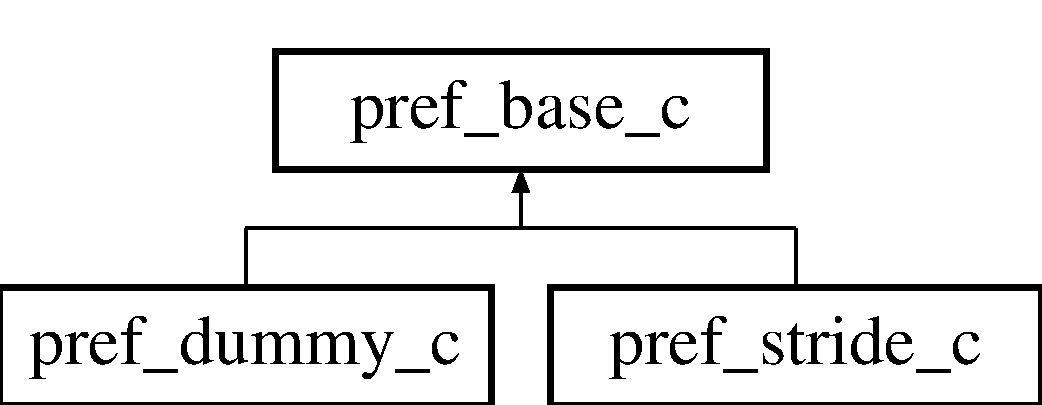
\includegraphics[height=2.000000cm]{classpref__base__c}
\end{center}
\end{figure}
\subsection*{Public Member Functions}
\begin{DoxyCompactItemize}
\item 
\hyperlink{classpref__base__c_a0b524a96fc04c9a07e2a11c7ebaf18e2}{pref\_\-base\_\-c} (\hyperlink{classmacsim__c}{macsim\_\-c} $\ast$simBase)
\item 
virtual \hyperlink{classpref__base__c_a4166198ff942f6a3e2af3b66ee16e5ff}{$\sim$pref\_\-base\_\-c} ()
\item 
virtual void \hyperlink{classpref__base__c_a404371f4c7e814352f3a6e0a1aeb4a9b}{init\_\-func} (int)=0
\item 
virtual void \hyperlink{classpref__base__c_af6f4f755ba7bc869f5bae908969eb969}{done\_\-func} ()=0
\item 
virtual void \hyperlink{classpref__base__c_a2b23d47a615b8bb700bd79104bcc1855}{l1\_\-miss\_\-func} (int tid, Addr addr, Addr pc, \hyperlink{classuop__c}{uop\_\-c} $\ast$uop)=0
\item 
virtual void \hyperlink{classpref__base__c_a39c3f0b35e3346133be50dbef1b5aa13}{l1\_\-hit\_\-func} (int tid, Addr addr, Addr pc, \hyperlink{classuop__c}{uop\_\-c} $\ast$uop)=0
\item 
virtual void \hyperlink{classpref__base__c_a0d54d273c63a4c78873632b6ae1953a7}{l1\_\-pref\_\-hit\_\-func} (int tid, Addr, Addr, \hyperlink{classuop__c}{uop\_\-c} $\ast$uop)=0
\item 
virtual void \hyperlink{classpref__base__c_afe9bb0f31178fc9acf2d35afe65d6cd0}{l2\_\-miss\_\-func} (int, Addr, Addr, \hyperlink{classuop__c}{uop\_\-c} $\ast$uop)=0
\item 
virtual void \hyperlink{classpref__base__c_acba9e1586edcddff8983b46c2147e80d}{l2\_\-hit\_\-func} (int, Addr, Addr, \hyperlink{classuop__c}{uop\_\-c} $\ast$uop)=0
\item 
virtual void \hyperlink{classpref__base__c_ae89bc30a1f74a1199bec721ca78197c1}{l2\_\-pref\_\-hit\_\-func} (int, Addr, Addr, \hyperlink{classuop__c}{uop\_\-c} $\ast$uop)=0
\end{DoxyCompactItemize}
\subsection*{Public Attributes}
\begin{DoxyCompactItemize}
\item 
bool \hyperlink{classpref__base__c_aae842be24193c5866e6a92b9706da71a}{init}
\item 
bool \hyperlink{classpref__base__c_a0b4fc71dbc57b37b14a3d690641095f8}{done}
\item 
bool \hyperlink{classpref__base__c_af3792920c5d8a07bb4b28d4a30d00450}{l1\_\-miss}
\item 
bool \hyperlink{classpref__base__c_a74726ac22c802880c289bf77dd7b6cca}{l1\_\-hit}
\item 
bool \hyperlink{classpref__base__c_ad687a452e183c6fa0d6dce6371a5dfae}{l1\_\-pref\_\-hit}
\item 
bool \hyperlink{classpref__base__c_a3c4a6b2464e480335b1e5776b4b69bf6}{l2\_\-miss}
\item 
bool \hyperlink{classpref__base__c_a75478fddf153aa4ae23fc7434307dda8}{l2\_\-hit}
\item 
bool \hyperlink{classpref__base__c_a3cd5ebbc80aeee89f7e4287b0ed930e3}{l2\_\-pref\_\-hit}
\item 
string \hyperlink{classpref__base__c_a65b7301bf63f68f8d6c7b893dffa3353}{name}
\item 
HWP\_\-Type \hyperlink{classpref__base__c_a6fb57b9239bf6a8241c0e3e8d67ba95b}{hwp\_\-type}
\item 
\hyperlink{structpref__info__s}{pref\_\-info\_\-s} $\ast$ \hyperlink{classpref__base__c_a4bcc37c2e993a745957630fa8ea8d8e2}{hwp\_\-info}
\item 
\hyperlink{classhwp__common__c}{hwp\_\-common\_\-c} $\ast$ \hyperlink{classpref__base__c_a7e56ec8eb84f475c224c86ceabf858d9}{hwp\_\-common}
\item 
bool \hyperlink{classpref__base__c_ad2b3adaf6b7ae24a519451a67cc4f57f}{knob\_\-enable}
\item 
int \hyperlink{classpref__base__c_ab0093a517b5e4f673a4c497af6ac0658}{core\_\-id}
\item 
int \hyperlink{classpref__base__c_a71a0797d8af664c87de0ebcf7fb36e96}{shift\_\-bit}
\end{DoxyCompactItemize}
\subsection*{Protected Attributes}
\begin{DoxyCompactItemize}
\item 
\hyperlink{classmacsim__c}{macsim\_\-c} $\ast$ \hyperlink{classpref__base__c_ab4840aa16085f9351c4acde5e8232ded}{m\_\-simBase}
\end{DoxyCompactItemize}
\subsection*{Friends}
\begin{DoxyCompactItemize}
\item 
\hypertarget{classpref__base__c_a8d09d4836ddc352da5be834d4969b647}{
class {\bfseries pref\_\-common\_\-c}}
\label{classpref__base__c_a8d09d4836ddc352da5be834d4969b647}

\end{DoxyCompactItemize}


\subsection{Detailed Description}
Hardware prefetcher base class. Prefetcher base class. Based on the event (dcache, L2 cache / miss, hit, pref\_\-hit), corresponding function will be called 

\subsection{Constructor \& Destructor Documentation}
\hypertarget{classpref__base__c_a0b524a96fc04c9a07e2a11c7ebaf18e2}{
\index{pref\_\-base\_\-c@{pref\_\-base\_\-c}!pref\_\-base\_\-c@{pref\_\-base\_\-c}}
\index{pref\_\-base\_\-c@{pref\_\-base\_\-c}!pref_base_c@{pref\_\-base\_\-c}}
\subsubsection[{pref\_\-base\_\-c}]{\setlength{\rightskip}{0pt plus 5cm}pref\_\-base\_\-c::pref\_\-base\_\-c (
\begin{DoxyParamCaption}
\item[{{\bf macsim\_\-c} $\ast$}]{ simBase}
\end{DoxyParamCaption}
)}}
\label{classpref__base__c_a0b524a96fc04c9a07e2a11c7ebaf18e2}
Constructor \hypertarget{classpref__base__c_a4166198ff942f6a3e2af3b66ee16e5ff}{
\index{pref\_\-base\_\-c@{pref\_\-base\_\-c}!$\sim$pref\_\-base\_\-c@{$\sim$pref\_\-base\_\-c}}
\index{$\sim$pref\_\-base\_\-c@{$\sim$pref\_\-base\_\-c}!pref_base_c@{pref\_\-base\_\-c}}
\subsubsection[{$\sim$pref\_\-base\_\-c}]{\setlength{\rightskip}{0pt plus 5cm}virtual pref\_\-base\_\-c::$\sim$pref\_\-base\_\-c (
\begin{DoxyParamCaption}
{}
\end{DoxyParamCaption}
)\hspace{0.3cm}{\ttfamily  \mbox{[}inline, virtual\mbox{]}}}}
\label{classpref__base__c_a4166198ff942f6a3e2af3b66ee16e5ff}
Virtual destructor 

\subsection{Member Function Documentation}
\hypertarget{classpref__base__c_af6f4f755ba7bc869f5bae908969eb969}{
\index{pref\_\-base\_\-c@{pref\_\-base\_\-c}!done\_\-func@{done\_\-func}}
\index{done\_\-func@{done\_\-func}!pref_base_c@{pref\_\-base\_\-c}}
\subsubsection[{done\_\-func}]{\setlength{\rightskip}{0pt plus 5cm}virtual void pref\_\-base\_\-c::done\_\-func (
\begin{DoxyParamCaption}
{}
\end{DoxyParamCaption}
)\hspace{0.3cm}{\ttfamily  \mbox{[}pure virtual\mbox{]}}}}
\label{classpref__base__c_af6f4f755ba7bc869f5bae908969eb969}
Done function : When a prefetch request is serviced, done\_\-func will be called. 

Implemented in \hyperlink{classpref__dummy__c_ac77e468dcd3b9bf7769acfb46a9e53b6}{pref\_\-dummy\_\-c}, and \hyperlink{classpref__stride__c_a147e597a5eb20dc3b903c3c5eaf8973b}{pref\_\-stride\_\-c}.

\hypertarget{classpref__base__c_a404371f4c7e814352f3a6e0a1aeb4a9b}{
\index{pref\_\-base\_\-c@{pref\_\-base\_\-c}!init\_\-func@{init\_\-func}}
\index{init\_\-func@{init\_\-func}!pref_base_c@{pref\_\-base\_\-c}}
\subsubsection[{init\_\-func}]{\setlength{\rightskip}{0pt plus 5cm}virtual void pref\_\-base\_\-c::init\_\-func (
\begin{DoxyParamCaption}
\item[{int}]{}
\end{DoxyParamCaption}
)\hspace{0.3cm}{\ttfamily  \mbox{[}pure virtual\mbox{]}}}}
\label{classpref__base__c_a404371f4c7e814352f3a6e0a1aeb4a9b}
Initialize function 

Implemented in \hyperlink{classpref__dummy__c_a369a5b5a5f05dc63781ddb9551f8a6ae}{pref\_\-dummy\_\-c}, and \hyperlink{classpref__stride__c_a09ed6d4a95388ec667244be7d977eea2}{pref\_\-stride\_\-c}.

\hypertarget{classpref__base__c_a39c3f0b35e3346133be50dbef1b5aa13}{
\index{pref\_\-base\_\-c@{pref\_\-base\_\-c}!l1\_\-hit\_\-func@{l1\_\-hit\_\-func}}
\index{l1\_\-hit\_\-func@{l1\_\-hit\_\-func}!pref_base_c@{pref\_\-base\_\-c}}
\subsubsection[{l1\_\-hit\_\-func}]{\setlength{\rightskip}{0pt plus 5cm}virtual void pref\_\-base\_\-c::l1\_\-hit\_\-func (
\begin{DoxyParamCaption}
\item[{int}]{ tid, }
\item[{Addr}]{ addr, }
\item[{Addr}]{ pc, }
\item[{{\bf uop\_\-c} $\ast$}]{ uop}
\end{DoxyParamCaption}
)\hspace{0.3cm}{\ttfamily  \mbox{[}pure virtual\mbox{]}}}}
\label{classpref__base__c_a39c3f0b35e3346133be50dbef1b5aa13}
L1 Cache hit event handler 

Implemented in \hyperlink{classpref__dummy__c_a48e578d6907b986e25b4abb59bca62f3}{pref\_\-dummy\_\-c}, and \hyperlink{classpref__stride__c_a9021353112572858151e53b6c96df0b8}{pref\_\-stride\_\-c}.

\hypertarget{classpref__base__c_a2b23d47a615b8bb700bd79104bcc1855}{
\index{pref\_\-base\_\-c@{pref\_\-base\_\-c}!l1\_\-miss\_\-func@{l1\_\-miss\_\-func}}
\index{l1\_\-miss\_\-func@{l1\_\-miss\_\-func}!pref_base_c@{pref\_\-base\_\-c}}
\subsubsection[{l1\_\-miss\_\-func}]{\setlength{\rightskip}{0pt plus 5cm}virtual void pref\_\-base\_\-c::l1\_\-miss\_\-func (
\begin{DoxyParamCaption}
\item[{int}]{ tid, }
\item[{Addr}]{ addr, }
\item[{Addr}]{ pc, }
\item[{{\bf uop\_\-c} $\ast$}]{ uop}
\end{DoxyParamCaption}
)\hspace{0.3cm}{\ttfamily  \mbox{[}pure virtual\mbox{]}}}}
\label{classpref__base__c_a2b23d47a615b8bb700bd79104bcc1855}
L1 Cache miss event handler 

Implemented in \hyperlink{classpref__dummy__c_a3ec5ae0af4500c1995fcaff75d2ed19e}{pref\_\-dummy\_\-c}, and \hyperlink{classpref__stride__c_a7a75dcfa0945e493306b41b7f7d807f6}{pref\_\-stride\_\-c}.

\hypertarget{classpref__base__c_a0d54d273c63a4c78873632b6ae1953a7}{
\index{pref\_\-base\_\-c@{pref\_\-base\_\-c}!l1\_\-pref\_\-hit\_\-func@{l1\_\-pref\_\-hit\_\-func}}
\index{l1\_\-pref\_\-hit\_\-func@{l1\_\-pref\_\-hit\_\-func}!pref_base_c@{pref\_\-base\_\-c}}
\subsubsection[{l1\_\-pref\_\-hit\_\-func}]{\setlength{\rightskip}{0pt plus 5cm}virtual void pref\_\-base\_\-c::l1\_\-pref\_\-hit\_\-func (
\begin{DoxyParamCaption}
\item[{int}]{ tid, }
\item[{Addr}]{, }
\item[{Addr}]{, }
\item[{{\bf uop\_\-c} $\ast$}]{ uop}
\end{DoxyParamCaption}
)\hspace{0.3cm}{\ttfamily  \mbox{[}pure virtual\mbox{]}}}}
\label{classpref__base__c_a0d54d273c63a4c78873632b6ae1953a7}
L1 Cache prefetch hit event handler 

Implemented in \hyperlink{classpref__dummy__c_ab3c2f14fdfaaa9d3e83c73ae1b2a461e}{pref\_\-dummy\_\-c}, and \hyperlink{classpref__stride__c_aeb8654a0fae97b42d1945d2b8f99c795}{pref\_\-stride\_\-c}.

\hypertarget{classpref__base__c_acba9e1586edcddff8983b46c2147e80d}{
\index{pref\_\-base\_\-c@{pref\_\-base\_\-c}!l2\_\-hit\_\-func@{l2\_\-hit\_\-func}}
\index{l2\_\-hit\_\-func@{l2\_\-hit\_\-func}!pref_base_c@{pref\_\-base\_\-c}}
\subsubsection[{l2\_\-hit\_\-func}]{\setlength{\rightskip}{0pt plus 5cm}virtual void pref\_\-base\_\-c::l2\_\-hit\_\-func (
\begin{DoxyParamCaption}
\item[{int}]{, }
\item[{Addr}]{, }
\item[{Addr}]{, }
\item[{{\bf uop\_\-c} $\ast$}]{ uop}
\end{DoxyParamCaption}
)\hspace{0.3cm}{\ttfamily  \mbox{[}pure virtual\mbox{]}}}}
\label{classpref__base__c_acba9e1586edcddff8983b46c2147e80d}
L2 Cache hit event handler 

Implemented in \hyperlink{classpref__dummy__c_a6c17bd9a59c598c78928d0f0b6a7ca59}{pref\_\-dummy\_\-c}, and \hyperlink{classpref__stride__c_a7dfd002eebf50de73efe93b53c033044}{pref\_\-stride\_\-c}.

\hypertarget{classpref__base__c_afe9bb0f31178fc9acf2d35afe65d6cd0}{
\index{pref\_\-base\_\-c@{pref\_\-base\_\-c}!l2\_\-miss\_\-func@{l2\_\-miss\_\-func}}
\index{l2\_\-miss\_\-func@{l2\_\-miss\_\-func}!pref_base_c@{pref\_\-base\_\-c}}
\subsubsection[{l2\_\-miss\_\-func}]{\setlength{\rightskip}{0pt plus 5cm}virtual void pref\_\-base\_\-c::l2\_\-miss\_\-func (
\begin{DoxyParamCaption}
\item[{int}]{, }
\item[{Addr}]{, }
\item[{Addr}]{, }
\item[{{\bf uop\_\-c} $\ast$}]{ uop}
\end{DoxyParamCaption}
)\hspace{0.3cm}{\ttfamily  \mbox{[}pure virtual\mbox{]}}}}
\label{classpref__base__c_afe9bb0f31178fc9acf2d35afe65d6cd0}
L2 Cache miss event handler 

Implemented in \hyperlink{classpref__dummy__c_a37f2c774aa8e532b6a285a14d4906c78}{pref\_\-dummy\_\-c}, and \hyperlink{classpref__stride__c_a4083ad3dba1bb8357c32f035a464de83}{pref\_\-stride\_\-c}.

\hypertarget{classpref__base__c_ae89bc30a1f74a1199bec721ca78197c1}{
\index{pref\_\-base\_\-c@{pref\_\-base\_\-c}!l2\_\-pref\_\-hit\_\-func@{l2\_\-pref\_\-hit\_\-func}}
\index{l2\_\-pref\_\-hit\_\-func@{l2\_\-pref\_\-hit\_\-func}!pref_base_c@{pref\_\-base\_\-c}}
\subsubsection[{l2\_\-pref\_\-hit\_\-func}]{\setlength{\rightskip}{0pt plus 5cm}virtual void pref\_\-base\_\-c::l2\_\-pref\_\-hit\_\-func (
\begin{DoxyParamCaption}
\item[{int}]{, }
\item[{Addr}]{, }
\item[{Addr}]{, }
\item[{{\bf uop\_\-c} $\ast$}]{ uop}
\end{DoxyParamCaption}
)\hspace{0.3cm}{\ttfamily  \mbox{[}pure virtual\mbox{]}}}}
\label{classpref__base__c_ae89bc30a1f74a1199bec721ca78197c1}
L2 Cache prefetch hit event handler 

Implemented in \hyperlink{classpref__dummy__c_abb864a062e8c7a489eb5edb227b3f543}{pref\_\-dummy\_\-c}, and \hyperlink{classpref__stride__c_acbaa296a61779db50bc2ff8b3807b434}{pref\_\-stride\_\-c}.



\subsection{Member Data Documentation}
\hypertarget{classpref__base__c_ab0093a517b5e4f673a4c497af6ac0658}{
\index{pref\_\-base\_\-c@{pref\_\-base\_\-c}!core\_\-id@{core\_\-id}}
\index{core\_\-id@{core\_\-id}!pref_base_c@{pref\_\-base\_\-c}}
\subsubsection[{core\_\-id}]{\setlength{\rightskip}{0pt plus 5cm}int {\bf pref\_\-base\_\-c::core\_\-id}}}
\label{classpref__base__c_ab0093a517b5e4f673a4c497af6ac0658}
core id \hypertarget{classpref__base__c_a0b4fc71dbc57b37b14a3d690641095f8}{
\index{pref\_\-base\_\-c@{pref\_\-base\_\-c}!done@{done}}
\index{done@{done}!pref_base_c@{pref\_\-base\_\-c}}
\subsubsection[{done}]{\setlength{\rightskip}{0pt plus 5cm}bool {\bf pref\_\-base\_\-c::done}}}
\label{classpref__base__c_a0b4fc71dbc57b37b14a3d690641095f8}
Enable done function \hypertarget{classpref__base__c_a7e56ec8eb84f475c224c86ceabf858d9}{
\index{pref\_\-base\_\-c@{pref\_\-base\_\-c}!hwp\_\-common@{hwp\_\-common}}
\index{hwp\_\-common@{hwp\_\-common}!pref_base_c@{pref\_\-base\_\-c}}
\subsubsection[{hwp\_\-common}]{\setlength{\rightskip}{0pt plus 5cm}{\bf hwp\_\-common\_\-c}$\ast$ {\bf pref\_\-base\_\-c::hwp\_\-common}}}
\label{classpref__base__c_a7e56ec8eb84f475c224c86ceabf858d9}
pointer to prefetcher framework \hypertarget{classpref__base__c_a4bcc37c2e993a745957630fa8ea8d8e2}{
\index{pref\_\-base\_\-c@{pref\_\-base\_\-c}!hwp\_\-info@{hwp\_\-info}}
\index{hwp\_\-info@{hwp\_\-info}!pref_base_c@{pref\_\-base\_\-c}}
\subsubsection[{hwp\_\-info}]{\setlength{\rightskip}{0pt plus 5cm}{\bf pref\_\-info\_\-s}$\ast$ {\bf pref\_\-base\_\-c::hwp\_\-info}}}
\label{classpref__base__c_a4bcc37c2e993a745957630fa8ea8d8e2}
prefetcher information structure \hypertarget{classpref__base__c_a6fb57b9239bf6a8241c0e3e8d67ba95b}{
\index{pref\_\-base\_\-c@{pref\_\-base\_\-c}!hwp\_\-type@{hwp\_\-type}}
\index{hwp\_\-type@{hwp\_\-type}!pref_base_c@{pref\_\-base\_\-c}}
\subsubsection[{hwp\_\-type}]{\setlength{\rightskip}{0pt plus 5cm}HWP\_\-Type {\bf pref\_\-base\_\-c::hwp\_\-type}}}
\label{classpref__base__c_a6fb57b9239bf6a8241c0e3e8d67ba95b}
prefetcher type \hypertarget{classpref__base__c_aae842be24193c5866e6a92b9706da71a}{
\index{pref\_\-base\_\-c@{pref\_\-base\_\-c}!init@{init}}
\index{init@{init}!pref_base_c@{pref\_\-base\_\-c}}
\subsubsection[{init}]{\setlength{\rightskip}{0pt plus 5cm}bool {\bf pref\_\-base\_\-c::init}}}
\label{classpref__base__c_aae842be24193c5866e6a92b9706da71a}
Enable init function \hypertarget{classpref__base__c_ad2b3adaf6b7ae24a519451a67cc4f57f}{
\index{pref\_\-base\_\-c@{pref\_\-base\_\-c}!knob\_\-enable@{knob\_\-enable}}
\index{knob\_\-enable@{knob\_\-enable}!pref_base_c@{pref\_\-base\_\-c}}
\subsubsection[{knob\_\-enable}]{\setlength{\rightskip}{0pt plus 5cm}bool {\bf pref\_\-base\_\-c::knob\_\-enable}}}
\label{classpref__base__c_ad2b3adaf6b7ae24a519451a67cc4f57f}
enable prefetcher \hypertarget{classpref__base__c_a74726ac22c802880c289bf77dd7b6cca}{
\index{pref\_\-base\_\-c@{pref\_\-base\_\-c}!l1\_\-hit@{l1\_\-hit}}
\index{l1\_\-hit@{l1\_\-hit}!pref_base_c@{pref\_\-base\_\-c}}
\subsubsection[{l1\_\-hit}]{\setlength{\rightskip}{0pt plus 5cm}bool {\bf pref\_\-base\_\-c::l1\_\-hit}}}
\label{classpref__base__c_a74726ac22c802880c289bf77dd7b6cca}
Enable L1 hit handler \hypertarget{classpref__base__c_af3792920c5d8a07bb4b28d4a30d00450}{
\index{pref\_\-base\_\-c@{pref\_\-base\_\-c}!l1\_\-miss@{l1\_\-miss}}
\index{l1\_\-miss@{l1\_\-miss}!pref_base_c@{pref\_\-base\_\-c}}
\subsubsection[{l1\_\-miss}]{\setlength{\rightskip}{0pt plus 5cm}bool {\bf pref\_\-base\_\-c::l1\_\-miss}}}
\label{classpref__base__c_af3792920c5d8a07bb4b28d4a30d00450}
Enable L1 miss handler \hypertarget{classpref__base__c_ad687a452e183c6fa0d6dce6371a5dfae}{
\index{pref\_\-base\_\-c@{pref\_\-base\_\-c}!l1\_\-pref\_\-hit@{l1\_\-pref\_\-hit}}
\index{l1\_\-pref\_\-hit@{l1\_\-pref\_\-hit}!pref_base_c@{pref\_\-base\_\-c}}
\subsubsection[{l1\_\-pref\_\-hit}]{\setlength{\rightskip}{0pt plus 5cm}bool {\bf pref\_\-base\_\-c::l1\_\-pref\_\-hit}}}
\label{classpref__base__c_ad687a452e183c6fa0d6dce6371a5dfae}
Enable L1 prefetch hit handler \hypertarget{classpref__base__c_a75478fddf153aa4ae23fc7434307dda8}{
\index{pref\_\-base\_\-c@{pref\_\-base\_\-c}!l2\_\-hit@{l2\_\-hit}}
\index{l2\_\-hit@{l2\_\-hit}!pref_base_c@{pref\_\-base\_\-c}}
\subsubsection[{l2\_\-hit}]{\setlength{\rightskip}{0pt plus 5cm}bool {\bf pref\_\-base\_\-c::l2\_\-hit}}}
\label{classpref__base__c_a75478fddf153aa4ae23fc7434307dda8}
Enable L2 hit handler \hypertarget{classpref__base__c_a3c4a6b2464e480335b1e5776b4b69bf6}{
\index{pref\_\-base\_\-c@{pref\_\-base\_\-c}!l2\_\-miss@{l2\_\-miss}}
\index{l2\_\-miss@{l2\_\-miss}!pref_base_c@{pref\_\-base\_\-c}}
\subsubsection[{l2\_\-miss}]{\setlength{\rightskip}{0pt plus 5cm}bool {\bf pref\_\-base\_\-c::l2\_\-miss}}}
\label{classpref__base__c_a3c4a6b2464e480335b1e5776b4b69bf6}
Enable L2 miss handler \hypertarget{classpref__base__c_a3cd5ebbc80aeee89f7e4287b0ed930e3}{
\index{pref\_\-base\_\-c@{pref\_\-base\_\-c}!l2\_\-pref\_\-hit@{l2\_\-pref\_\-hit}}
\index{l2\_\-pref\_\-hit@{l2\_\-pref\_\-hit}!pref_base_c@{pref\_\-base\_\-c}}
\subsubsection[{l2\_\-pref\_\-hit}]{\setlength{\rightskip}{0pt plus 5cm}bool {\bf pref\_\-base\_\-c::l2\_\-pref\_\-hit}}}
\label{classpref__base__c_a3cd5ebbc80aeee89f7e4287b0ed930e3}
Enable L2 prefetch hit handler \hypertarget{classpref__base__c_ab4840aa16085f9351c4acde5e8232ded}{
\index{pref\_\-base\_\-c@{pref\_\-base\_\-c}!m\_\-simBase@{m\_\-simBase}}
\index{m\_\-simBase@{m\_\-simBase}!pref_base_c@{pref\_\-base\_\-c}}
\subsubsection[{m\_\-simBase}]{\setlength{\rightskip}{0pt plus 5cm}{\bf macsim\_\-c}$\ast$ {\bf pref\_\-base\_\-c::m\_\-simBase}\hspace{0.3cm}{\ttfamily  \mbox{[}protected\mbox{]}}}}
\label{classpref__base__c_ab4840aa16085f9351c4acde5e8232ded}
\hyperlink{classmacsim__c}{macsim\_\-c} base class for simulation globals \hypertarget{classpref__base__c_a65b7301bf63f68f8d6c7b893dffa3353}{
\index{pref\_\-base\_\-c@{pref\_\-base\_\-c}!name@{name}}
\index{name@{name}!pref_base_c@{pref\_\-base\_\-c}}
\subsubsection[{name}]{\setlength{\rightskip}{0pt plus 5cm}string {\bf pref\_\-base\_\-c::name}}}
\label{classpref__base__c_a65b7301bf63f68f8d6c7b893dffa3353}
prefetcher name \hypertarget{classpref__base__c_a71a0797d8af664c87de0ebcf7fb36e96}{
\index{pref\_\-base\_\-c@{pref\_\-base\_\-c}!shift\_\-bit@{shift\_\-bit}}
\index{shift\_\-bit@{shift\_\-bit}!pref_base_c@{pref\_\-base\_\-c}}
\subsubsection[{shift\_\-bit}]{\setlength{\rightskip}{0pt plus 5cm}int {\bf pref\_\-base\_\-c::shift\_\-bit}}}
\label{classpref__base__c_a71a0797d8af664c87de0ebcf7fb36e96}
cache line address shift bits 

The documentation for this class was generated from the following files:\begin{DoxyCompactItemize}
\item 
pref.h\item 
pref.cc\end{DoxyCompactItemize}

\hypertarget{classpref__dummy__c}{
\section{pref\_\-dummy\_\-c Class Reference}
\label{classpref__dummy__c}\index{pref\_\-dummy\_\-c@{pref\_\-dummy\_\-c}}
}


Dummy prefetcher class.  




{\ttfamily \#include $<$pref.h$>$}

Inheritance diagram for pref\_\-dummy\_\-c:\begin{figure}[H]
\begin{center}
\leavevmode
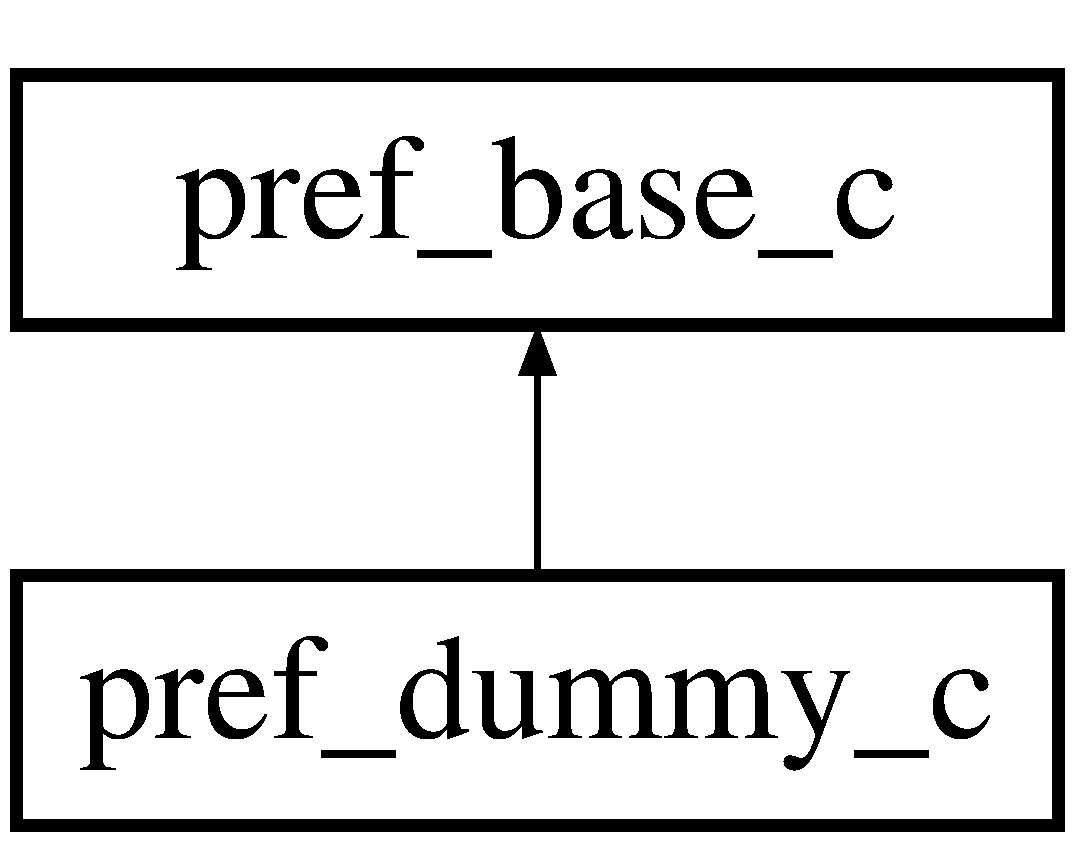
\includegraphics[height=2.000000cm]{classpref__dummy__c}
\end{center}
\end{figure}
\subsection*{Public Member Functions}
\begin{DoxyCompactItemize}
\item 
\hyperlink{classpref__dummy__c_a2c5d6804fd5ed823991bda4fe5fb3531}{pref\_\-dummy\_\-c} (\hyperlink{classmacsim__c}{macsim\_\-c} $\ast$simBase)
\item 
\hyperlink{classpref__dummy__c_abad511b20db2326cf78296d43b5315fc}{$\sim$pref\_\-dummy\_\-c} ()
\item 
void \hyperlink{classpref__dummy__c_a369a5b5a5f05dc63781ddb9551f8a6ae}{init\_\-func} (int a)
\item 
void \hyperlink{classpref__dummy__c_ac77e468dcd3b9bf7769acfb46a9e53b6}{done\_\-func} ()
\item 
void \hyperlink{classpref__dummy__c_a3ec5ae0af4500c1995fcaff75d2ed19e}{l1\_\-miss\_\-func} (int a, Addr b, Addr c, \hyperlink{classuop__c}{uop\_\-c} $\ast$d)
\item 
void \hyperlink{classpref__dummy__c_a48e578d6907b986e25b4abb59bca62f3}{l1\_\-hit\_\-func} (int a, Addr b, Addr c, \hyperlink{classuop__c}{uop\_\-c} $\ast$d)
\item 
void \hyperlink{classpref__dummy__c_ab3c2f14fdfaaa9d3e83c73ae1b2a461e}{l1\_\-pref\_\-hit\_\-func} (int a, Addr b, Addr c, \hyperlink{classuop__c}{uop\_\-c} $\ast$d)
\item 
void \hyperlink{classpref__dummy__c_a37f2c774aa8e532b6a285a14d4906c78}{l2\_\-miss\_\-func} (int a, Addr b, Addr c, \hyperlink{classuop__c}{uop\_\-c} $\ast$d)
\item 
void \hyperlink{classpref__dummy__c_a6c17bd9a59c598c78928d0f0b6a7ca59}{l2\_\-hit\_\-func} (int a, Addr b, Addr c, \hyperlink{classuop__c}{uop\_\-c} $\ast$d)
\item 
void \hyperlink{classpref__dummy__c_abb864a062e8c7a489eb5edb227b3f543}{l2\_\-pref\_\-hit\_\-func} (int a, Addr b, Addr c, \hyperlink{classuop__c}{uop\_\-c} $\ast$d)
\end{DoxyCompactItemize}


\subsection{Detailed Description}
Dummy prefetcher class. Show how to use base prefetcher class 

\subsection{Constructor \& Destructor Documentation}
\hypertarget{classpref__dummy__c_a2c5d6804fd5ed823991bda4fe5fb3531}{
\index{pref\_\-dummy\_\-c@{pref\_\-dummy\_\-c}!pref\_\-dummy\_\-c@{pref\_\-dummy\_\-c}}
\index{pref\_\-dummy\_\-c@{pref\_\-dummy\_\-c}!pref_dummy_c@{pref\_\-dummy\_\-c}}
\subsubsection[{pref\_\-dummy\_\-c}]{\setlength{\rightskip}{0pt plus 5cm}pref\_\-dummy\_\-c::pref\_\-dummy\_\-c (
\begin{DoxyParamCaption}
\item[{{\bf macsim\_\-c} $\ast$}]{ simBase}
\end{DoxyParamCaption}
)\hspace{0.3cm}{\ttfamily  \mbox{[}inline\mbox{]}}}}
\label{classpref__dummy__c_a2c5d6804fd5ed823991bda4fe5fb3531}
Constructor \hypertarget{classpref__dummy__c_abad511b20db2326cf78296d43b5315fc}{
\index{pref\_\-dummy\_\-c@{pref\_\-dummy\_\-c}!$\sim$pref\_\-dummy\_\-c@{$\sim$pref\_\-dummy\_\-c}}
\index{$\sim$pref\_\-dummy\_\-c@{$\sim$pref\_\-dummy\_\-c}!pref_dummy_c@{pref\_\-dummy\_\-c}}
\subsubsection[{$\sim$pref\_\-dummy\_\-c}]{\setlength{\rightskip}{0pt plus 5cm}pref\_\-dummy\_\-c::$\sim$pref\_\-dummy\_\-c (
\begin{DoxyParamCaption}
{}
\end{DoxyParamCaption}
)\hspace{0.3cm}{\ttfamily  \mbox{[}inline\mbox{]}}}}
\label{classpref__dummy__c_abad511b20db2326cf78296d43b5315fc}
Destructor 

\subsection{Member Function Documentation}
\hypertarget{classpref__dummy__c_ac77e468dcd3b9bf7769acfb46a9e53b6}{
\index{pref\_\-dummy\_\-c@{pref\_\-dummy\_\-c}!done\_\-func@{done\_\-func}}
\index{done\_\-func@{done\_\-func}!pref_dummy_c@{pref\_\-dummy\_\-c}}
\subsubsection[{done\_\-func}]{\setlength{\rightskip}{0pt plus 5cm}void pref\_\-dummy\_\-c::done\_\-func (
\begin{DoxyParamCaption}
{}
\end{DoxyParamCaption}
)\hspace{0.3cm}{\ttfamily  \mbox{[}inline, virtual\mbox{]}}}}
\label{classpref__dummy__c_ac77e468dcd3b9bf7769acfb46a9e53b6}
Done function : When a prefetch request is serviced, done\_\-func will be called. 

Implements \hyperlink{classpref__base__c_af6f4f755ba7bc869f5bae908969eb969}{pref\_\-base\_\-c}.

\hypertarget{classpref__dummy__c_a369a5b5a5f05dc63781ddb9551f8a6ae}{
\index{pref\_\-dummy\_\-c@{pref\_\-dummy\_\-c}!init\_\-func@{init\_\-func}}
\index{init\_\-func@{init\_\-func}!pref_dummy_c@{pref\_\-dummy\_\-c}}
\subsubsection[{init\_\-func}]{\setlength{\rightskip}{0pt plus 5cm}void pref\_\-dummy\_\-c::init\_\-func (
\begin{DoxyParamCaption}
\item[{int}]{ a}
\end{DoxyParamCaption}
)\hspace{0.3cm}{\ttfamily  \mbox{[}inline, virtual\mbox{]}}}}
\label{classpref__dummy__c_a369a5b5a5f05dc63781ddb9551f8a6ae}
Initialize function 

Implements \hyperlink{classpref__base__c_a404371f4c7e814352f3a6e0a1aeb4a9b}{pref\_\-base\_\-c}.

\hypertarget{classpref__dummy__c_a48e578d6907b986e25b4abb59bca62f3}{
\index{pref\_\-dummy\_\-c@{pref\_\-dummy\_\-c}!l1\_\-hit\_\-func@{l1\_\-hit\_\-func}}
\index{l1\_\-hit\_\-func@{l1\_\-hit\_\-func}!pref_dummy_c@{pref\_\-dummy\_\-c}}
\subsubsection[{l1\_\-hit\_\-func}]{\setlength{\rightskip}{0pt plus 5cm}void pref\_\-dummy\_\-c::l1\_\-hit\_\-func (
\begin{DoxyParamCaption}
\item[{int}]{ a, }
\item[{Addr}]{ b, }
\item[{Addr}]{ c, }
\item[{{\bf uop\_\-c} $\ast$}]{ d}
\end{DoxyParamCaption}
)\hspace{0.3cm}{\ttfamily  \mbox{[}inline, virtual\mbox{]}}}}
\label{classpref__dummy__c_a48e578d6907b986e25b4abb59bca62f3}
L1 Cache hit event handler 

Implements \hyperlink{classpref__base__c_a39c3f0b35e3346133be50dbef1b5aa13}{pref\_\-base\_\-c}.

\hypertarget{classpref__dummy__c_a3ec5ae0af4500c1995fcaff75d2ed19e}{
\index{pref\_\-dummy\_\-c@{pref\_\-dummy\_\-c}!l1\_\-miss\_\-func@{l1\_\-miss\_\-func}}
\index{l1\_\-miss\_\-func@{l1\_\-miss\_\-func}!pref_dummy_c@{pref\_\-dummy\_\-c}}
\subsubsection[{l1\_\-miss\_\-func}]{\setlength{\rightskip}{0pt plus 5cm}void pref\_\-dummy\_\-c::l1\_\-miss\_\-func (
\begin{DoxyParamCaption}
\item[{int}]{ a, }
\item[{Addr}]{ b, }
\item[{Addr}]{ c, }
\item[{{\bf uop\_\-c} $\ast$}]{ d}
\end{DoxyParamCaption}
)\hspace{0.3cm}{\ttfamily  \mbox{[}inline, virtual\mbox{]}}}}
\label{classpref__dummy__c_a3ec5ae0af4500c1995fcaff75d2ed19e}
L1 Cache miss event handler 

Implements \hyperlink{classpref__base__c_a2b23d47a615b8bb700bd79104bcc1855}{pref\_\-base\_\-c}.

\hypertarget{classpref__dummy__c_ab3c2f14fdfaaa9d3e83c73ae1b2a461e}{
\index{pref\_\-dummy\_\-c@{pref\_\-dummy\_\-c}!l1\_\-pref\_\-hit\_\-func@{l1\_\-pref\_\-hit\_\-func}}
\index{l1\_\-pref\_\-hit\_\-func@{l1\_\-pref\_\-hit\_\-func}!pref_dummy_c@{pref\_\-dummy\_\-c}}
\subsubsection[{l1\_\-pref\_\-hit\_\-func}]{\setlength{\rightskip}{0pt plus 5cm}void pref\_\-dummy\_\-c::l1\_\-pref\_\-hit\_\-func (
\begin{DoxyParamCaption}
\item[{int}]{ a, }
\item[{Addr}]{ b, }
\item[{Addr}]{ c, }
\item[{{\bf uop\_\-c} $\ast$}]{ d}
\end{DoxyParamCaption}
)\hspace{0.3cm}{\ttfamily  \mbox{[}inline, virtual\mbox{]}}}}
\label{classpref__dummy__c_ab3c2f14fdfaaa9d3e83c73ae1b2a461e}
L1 Cache prefetch hit event handler 

Implements \hyperlink{classpref__base__c_a0d54d273c63a4c78873632b6ae1953a7}{pref\_\-base\_\-c}.

\hypertarget{classpref__dummy__c_a6c17bd9a59c598c78928d0f0b6a7ca59}{
\index{pref\_\-dummy\_\-c@{pref\_\-dummy\_\-c}!l2\_\-hit\_\-func@{l2\_\-hit\_\-func}}
\index{l2\_\-hit\_\-func@{l2\_\-hit\_\-func}!pref_dummy_c@{pref\_\-dummy\_\-c}}
\subsubsection[{l2\_\-hit\_\-func}]{\setlength{\rightskip}{0pt plus 5cm}void pref\_\-dummy\_\-c::l2\_\-hit\_\-func (
\begin{DoxyParamCaption}
\item[{int}]{ a, }
\item[{Addr}]{ b, }
\item[{Addr}]{ c, }
\item[{{\bf uop\_\-c} $\ast$}]{ d}
\end{DoxyParamCaption}
)\hspace{0.3cm}{\ttfamily  \mbox{[}inline, virtual\mbox{]}}}}
\label{classpref__dummy__c_a6c17bd9a59c598c78928d0f0b6a7ca59}
L2 Cache hit event handler 

Implements \hyperlink{classpref__base__c_acba9e1586edcddff8983b46c2147e80d}{pref\_\-base\_\-c}.

\hypertarget{classpref__dummy__c_a37f2c774aa8e532b6a285a14d4906c78}{
\index{pref\_\-dummy\_\-c@{pref\_\-dummy\_\-c}!l2\_\-miss\_\-func@{l2\_\-miss\_\-func}}
\index{l2\_\-miss\_\-func@{l2\_\-miss\_\-func}!pref_dummy_c@{pref\_\-dummy\_\-c}}
\subsubsection[{l2\_\-miss\_\-func}]{\setlength{\rightskip}{0pt plus 5cm}void pref\_\-dummy\_\-c::l2\_\-miss\_\-func (
\begin{DoxyParamCaption}
\item[{int}]{ a, }
\item[{Addr}]{ b, }
\item[{Addr}]{ c, }
\item[{{\bf uop\_\-c} $\ast$}]{ d}
\end{DoxyParamCaption}
)\hspace{0.3cm}{\ttfamily  \mbox{[}inline, virtual\mbox{]}}}}
\label{classpref__dummy__c_a37f2c774aa8e532b6a285a14d4906c78}
L2 Cache miss event handler 

Implements \hyperlink{classpref__base__c_afe9bb0f31178fc9acf2d35afe65d6cd0}{pref\_\-base\_\-c}.

\hypertarget{classpref__dummy__c_abb864a062e8c7a489eb5edb227b3f543}{
\index{pref\_\-dummy\_\-c@{pref\_\-dummy\_\-c}!l2\_\-pref\_\-hit\_\-func@{l2\_\-pref\_\-hit\_\-func}}
\index{l2\_\-pref\_\-hit\_\-func@{l2\_\-pref\_\-hit\_\-func}!pref_dummy_c@{pref\_\-dummy\_\-c}}
\subsubsection[{l2\_\-pref\_\-hit\_\-func}]{\setlength{\rightskip}{0pt plus 5cm}void pref\_\-dummy\_\-c::l2\_\-pref\_\-hit\_\-func (
\begin{DoxyParamCaption}
\item[{int}]{ a, }
\item[{Addr}]{ b, }
\item[{Addr}]{ c, }
\item[{{\bf uop\_\-c} $\ast$}]{ d}
\end{DoxyParamCaption}
)\hspace{0.3cm}{\ttfamily  \mbox{[}inline, virtual\mbox{]}}}}
\label{classpref__dummy__c_abb864a062e8c7a489eb5edb227b3f543}
L2 Cache prefetch hit event handler 

Implements \hyperlink{classpref__base__c_ae89bc30a1f74a1199bec721ca78197c1}{pref\_\-base\_\-c}.



The documentation for this class was generated from the following file:\begin{DoxyCompactItemize}
\item 
pref.h\end{DoxyCompactItemize}

\hypertarget{classpref__factory__c}{
\section{pref\_\-factory\_\-c Class Reference}
\label{classpref__factory__c}\index{pref\_\-factory\_\-c@{pref\_\-factory\_\-c}}
}


pref policy factory Hardware prefetcher factory class : allocate prefetchers based on the configuration  




{\ttfamily \#include $<$pref\_\-factory.h$>$}

\subsection*{Public Member Functions}
\begin{DoxyCompactItemize}
\item 
\hyperlink{classpref__factory__c_a63f9a6dc8a6e7a2ebe3d73a47aa4aec2}{pref\_\-factory\_\-c} ()
\item 
\hyperlink{classpref__factory__c_a0a361d32320dfca170d738e8f4db0fd5}{$\sim$pref\_\-factory\_\-c} ()
\item 
void \hyperlink{classpref__factory__c_a7be154a97910948c1bb5fba5320940ba}{register\_\-class} (function$<$ void(vector$<$ \hyperlink{classpref__base__c}{pref\_\-base\_\-c} $\ast$ $>$ \&, \hyperlink{classhwp__common__c}{hwp\_\-common\_\-c} $\ast$, Unit\_\-Type, \hyperlink{classmacsim__c}{macsim\_\-c} $\ast$)$>$)
\item 
void \hyperlink{classpref__factory__c_aafb1c0a0160526b23c8e17285f76ce57}{allocate\_\-pref} (vector$<$ \hyperlink{classpref__base__c}{pref\_\-base\_\-c} $\ast$ $>$ \&, \hyperlink{classhwp__common__c}{hwp\_\-common\_\-c} $\ast$, Unit\_\-Type, \hyperlink{classmacsim__c}{macsim\_\-c} $\ast$)
\end{DoxyCompactItemize}
\subsection*{Static Public Member Functions}
\begin{DoxyCompactItemize}
\item 
static \hyperlink{classpref__factory__c}{pref\_\-factory\_\-c} $\ast$ \hyperlink{classpref__factory__c_a0aa0e3bd69c625e9b1ce80a7210b1b7a}{get} ()
\end{DoxyCompactItemize}
\subsection*{Static Public Attributes}
\begin{DoxyCompactItemize}
\item 
static \hyperlink{classpref__factory__c}{pref\_\-factory\_\-c} $\ast$ \hyperlink{classpref__factory__c_a8d68a36f77d53450d4dabb477f99faf5}{instance} = 0
\end{DoxyCompactItemize}
\subsection*{Private Attributes}
\begin{DoxyCompactItemize}
\item 
list$<$ function$<$ void(vector$<$ \hyperlink{classpref__base__c}{pref\_\-base\_\-c} $\ast$ $>$ \&, \hyperlink{classhwp__common__c}{hwp\_\-common\_\-c} $\ast$, Unit\_\-Type, \hyperlink{classmacsim__c}{macsim\_\-c} $\ast$)$>$ \hyperlink{classpref__factory__c_a6a70d54b0cf3cd76600a3060d05dfb49}{m\_\-func\_\-table} )
\end{DoxyCompactItemize}


\subsection{Detailed Description}
pref policy factory Hardware prefetcher factory class : allocate prefetchers based on the configuration 

\subsection{Constructor \& Destructor Documentation}
\hypertarget{classpref__factory__c_a63f9a6dc8a6e7a2ebe3d73a47aa4aec2}{
\index{pref\_\-factory\_\-c@{pref\_\-factory\_\-c}!pref\_\-factory\_\-c@{pref\_\-factory\_\-c}}
\index{pref\_\-factory\_\-c@{pref\_\-factory\_\-c}!pref_factory_c@{pref\_\-factory\_\-c}}
\subsubsection[{pref\_\-factory\_\-c}]{\setlength{\rightskip}{0pt plus 5cm}pref\_\-factory\_\-c::pref\_\-factory\_\-c (
\begin{DoxyParamCaption}
{}
\end{DoxyParamCaption}
)}}
\label{classpref__factory__c_a63f9a6dc8a6e7a2ebe3d73a47aa4aec2}
Constructor \hypertarget{classpref__factory__c_a0a361d32320dfca170d738e8f4db0fd5}{
\index{pref\_\-factory\_\-c@{pref\_\-factory\_\-c}!$\sim$pref\_\-factory\_\-c@{$\sim$pref\_\-factory\_\-c}}
\index{$\sim$pref\_\-factory\_\-c@{$\sim$pref\_\-factory\_\-c}!pref_factory_c@{pref\_\-factory\_\-c}}
\subsubsection[{$\sim$pref\_\-factory\_\-c}]{\setlength{\rightskip}{0pt plus 5cm}pref\_\-factory\_\-c::$\sim$pref\_\-factory\_\-c (
\begin{DoxyParamCaption}
{}
\end{DoxyParamCaption}
)}}
\label{classpref__factory__c_a0a361d32320dfca170d738e8f4db0fd5}
Destructor 

\subsection{Member Function Documentation}
\hypertarget{classpref__factory__c_aafb1c0a0160526b23c8e17285f76ce57}{
\index{pref\_\-factory\_\-c@{pref\_\-factory\_\-c}!allocate\_\-pref@{allocate\_\-pref}}
\index{allocate\_\-pref@{allocate\_\-pref}!pref_factory_c@{pref\_\-factory\_\-c}}
\subsubsection[{allocate\_\-pref}]{\setlength{\rightskip}{0pt plus 5cm}void pref\_\-factory\_\-c::allocate\_\-pref (
\begin{DoxyParamCaption}
\item[{vector$<$ {\bf pref\_\-base\_\-c} $\ast$ $>$ \&}]{ pref\_\-table, }
\item[{{\bf hwp\_\-common\_\-c} $\ast$}]{ hcc, }
\item[{Unit\_\-Type}]{ type, }
\item[{{\bf macsim\_\-c} $\ast$}]{ simBase}
\end{DoxyParamCaption}
)}}
\label{classpref__factory__c_aafb1c0a0160526b23c8e17285f76ce57}
Allocate hardware prefetchers which are registerd \hypertarget{classpref__factory__c_a0aa0e3bd69c625e9b1ce80a7210b1b7a}{
\index{pref\_\-factory\_\-c@{pref\_\-factory\_\-c}!get@{get}}
\index{get@{get}!pref_factory_c@{pref\_\-factory\_\-c}}
\subsubsection[{get}]{\setlength{\rightskip}{0pt plus 5cm}{\bf pref\_\-factory\_\-c} $\ast$ pref\_\-factory\_\-c::get (
\begin{DoxyParamCaption}
{}
\end{DoxyParamCaption}
)\hspace{0.3cm}{\ttfamily  \mbox{[}static\mbox{]}}}}
\label{classpref__factory__c_a0aa0e3bd69c625e9b1ce80a7210b1b7a}
Get singleton prefetch factory object \hypertarget{classpref__factory__c_a7be154a97910948c1bb5fba5320940ba}{
\index{pref\_\-factory\_\-c@{pref\_\-factory\_\-c}!register\_\-class@{register\_\-class}}
\index{register\_\-class@{register\_\-class}!pref_factory_c@{pref\_\-factory\_\-c}}
\subsubsection[{register\_\-class}]{\setlength{\rightskip}{0pt plus 5cm}void pref\_\-factory\_\-c::register\_\-class (
\begin{DoxyParamCaption}
\item[{function$<$ void(vector$<$ {\bf pref\_\-base\_\-c} $\ast$ $>$ \&, {\bf hwp\_\-common\_\-c} $\ast$, Unit\_\-Type, {\bf macsim\_\-c} $\ast$)$>$}]{ func}
\end{DoxyParamCaption}
)}}
\label{classpref__factory__c_a7be154a97910948c1bb5fba5320940ba}
Register a new hardware prefetcher class 

\subsection{Member Data Documentation}
\hypertarget{classpref__factory__c_a8d68a36f77d53450d4dabb477f99faf5}{
\index{pref\_\-factory\_\-c@{pref\_\-factory\_\-c}!instance@{instance}}
\index{instance@{instance}!pref_factory_c@{pref\_\-factory\_\-c}}
\subsubsection[{instance}]{\setlength{\rightskip}{0pt plus 5cm}{\bf pref\_\-factory\_\-c} $\ast$ {\bf pref\_\-factory\_\-c::instance} = 0\hspace{0.3cm}{\ttfamily  \mbox{[}static\mbox{]}}}}
\label{classpref__factory__c_a8d68a36f77d53450d4dabb477f99faf5}
Singleton factory \hypertarget{classpref__factory__c_a6a70d54b0cf3cd76600a3060d05dfb49}{
\index{pref\_\-factory\_\-c@{pref\_\-factory\_\-c}!m\_\-func\_\-table@{m\_\-func\_\-table}}
\index{m\_\-func\_\-table@{m\_\-func\_\-table}!pref_factory_c@{pref\_\-factory\_\-c}}
\subsubsection[{m\_\-func\_\-table}]{\setlength{\rightskip}{0pt plus 5cm}list$<$function$<$void (vector$<${\bf pref\_\-base\_\-c} $\ast$$>$ \&, {\bf hwp\_\-common\_\-c} $\ast$, Unit\_\-Type, {\bf macsim\_\-c}$\ast$)$>$  {\bf pref\_\-factory\_\-c::m\_\-func\_\-table})\hspace{0.3cm}{\ttfamily  \mbox{[}private\mbox{]}}}}
\label{classpref__factory__c_a6a70d54b0cf3cd76600a3060d05dfb49}
wrapper function table 

The documentation for this class was generated from the following files:\begin{DoxyCompactItemize}
\item 
pref\_\-factory.h\item 
pref\_\-factory.cc\end{DoxyCompactItemize}

\hypertarget{structpref__info__s}{
\section{pref\_\-info\_\-s Struct Reference}
\label{structpref__info__s}\index{pref\_\-info\_\-s@{pref\_\-info\_\-s}}
}


Hardware prefetcher structure (information, stats).  




{\ttfamily \#include $<$pref\_\-common.h$>$}

\subsection*{Public Attributes}
\begin{DoxyCompactItemize}
\item 
uns8 \hyperlink{structpref__info__s_aa751364dd397a33cd7ffdea42cbda8c0}{id}
\item 
bool \hyperlink{structpref__info__s_a76baaa162c64c556fad1f2f07cc11767}{enabled}
\item 
int \hyperlink{structpref__info__s_ad62caa3f68f6e5919b28dc207c46dfab}{priority}
\item 
Counter \hyperlink{structpref__info__s_a9b968c9aebf995d652f9f967eb7e5971}{useful}
\item 
Counter \hyperlink{structpref__info__s_a5c781e0f70693480da17b433e11d0132}{sent}
\item 
Counter \hyperlink{structpref__info__s_a2a55ea02b1cd31145a910e43a5ab74c0}{late}
\item 
Counter \hyperlink{structpref__info__s_ab196c66d3acfbe4309c4a6cc8fc565d5}{curr\_\-useful}
\item 
Counter \hyperlink{structpref__info__s_abc0afd16ea57472bdc0f79079cd3dc40}{curr\_\-sent}
\item 
Counter \hyperlink{structpref__info__s_ad21578ee3356e797bd0ebb5b3e61cbf5}{curr\_\-late}
\item 
Counter \hyperlink{structpref__info__s_a82eadd56d553c03fafdc8fa1349ee47d}{hybrid\_\-lastuseful}
\item 
Counter \hyperlink{structpref__info__s_a2e6f9ffea31a7a3dcb4b23d36b857dae}{hybrid\_\-lastsent}
\item 
Addr \hyperlink{structpref__info__s_a98609e4e7376f3fae20054c99feee11a}{trackers} \mbox{[}PREF\_\-TRACKERS\_\-NUM\mbox{]}
\item 
bool \hyperlink{structpref__info__s_a3c85c80bea8f5a3acbeb18316d8c912d}{trackers\_\-used} \mbox{[}PREF\_\-TRACKERS\_\-NUM\mbox{]}
\item 
int \hyperlink{structpref__info__s_a0c42749d820824d50ada89d498523f29}{track\_\-num}
\item 
Counter \hyperlink{structpref__info__s_a1151a69f70f1518d9223e15d91479300}{track\_\-lastsample\_\-cycle}
\item 
Counter \hyperlink{structpref__info__s_aa709dbfe970425b137e63b8376792392}{trackhist} \mbox{[}10\mbox{]}\mbox{[}PREF\_\-TRACKERS\_\-NUM\mbox{]}
\item 
Counter \hyperlink{structpref__info__s_a84a8db7783a6a9ae781fc5e5ee66b9da}{prefhit\_\-count}
\item 
uns \hyperlink{structpref__info__s_a99fd5a2733a16f8e4c89a91a87d219da}{dyn\_\-degree}
\end{DoxyCompactItemize}


\subsection{Detailed Description}
Hardware prefetcher structure (information, stats). 

\subsection{Member Data Documentation}
\hypertarget{structpref__info__s_ad21578ee3356e797bd0ebb5b3e61cbf5}{
\index{pref\_\-info\_\-s@{pref\_\-info\_\-s}!curr\_\-late@{curr\_\-late}}
\index{curr\_\-late@{curr\_\-late}!pref_info_s@{pref\_\-info\_\-s}}
\subsubsection[{curr\_\-late}]{\setlength{\rightskip}{0pt plus 5cm}Counter {\bf pref\_\-info\_\-s::curr\_\-late}}}
\label{structpref__info__s_ad21578ee3356e797bd0ebb5b3e61cbf5}
num of current period late prefetches \hypertarget{structpref__info__s_abc0afd16ea57472bdc0f79079cd3dc40}{
\index{pref\_\-info\_\-s@{pref\_\-info\_\-s}!curr\_\-sent@{curr\_\-sent}}
\index{curr\_\-sent@{curr\_\-sent}!pref_info_s@{pref\_\-info\_\-s}}
\subsubsection[{curr\_\-sent}]{\setlength{\rightskip}{0pt plus 5cm}Counter {\bf pref\_\-info\_\-s::curr\_\-sent}}}
\label{structpref__info__s_abc0afd16ea57472bdc0f79079cd3dc40}
num of current period sent prefetches \hypertarget{structpref__info__s_ab196c66d3acfbe4309c4a6cc8fc565d5}{
\index{pref\_\-info\_\-s@{pref\_\-info\_\-s}!curr\_\-useful@{curr\_\-useful}}
\index{curr\_\-useful@{curr\_\-useful}!pref_info_s@{pref\_\-info\_\-s}}
\subsubsection[{curr\_\-useful}]{\setlength{\rightskip}{0pt plus 5cm}Counter {\bf pref\_\-info\_\-s::curr\_\-useful}}}
\label{structpref__info__s_ab196c66d3acfbe4309c4a6cc8fc565d5}
num of current period Useful prefetches \hypertarget{structpref__info__s_a99fd5a2733a16f8e4c89a91a87d219da}{
\index{pref\_\-info\_\-s@{pref\_\-info\_\-s}!dyn\_\-degree@{dyn\_\-degree}}
\index{dyn\_\-degree@{dyn\_\-degree}!pref_info_s@{pref\_\-info\_\-s}}
\subsubsection[{dyn\_\-degree}]{\setlength{\rightskip}{0pt plus 5cm}uns {\bf pref\_\-info\_\-s::dyn\_\-degree}}}
\label{structpref__info__s_a99fd5a2733a16f8e4c89a91a87d219da}
dynamic prefetch degree \hypertarget{structpref__info__s_a76baaa162c64c556fad1f2f07cc11767}{
\index{pref\_\-info\_\-s@{pref\_\-info\_\-s}!enabled@{enabled}}
\index{enabled@{enabled}!pref_info_s@{pref\_\-info\_\-s}}
\subsubsection[{enabled}]{\setlength{\rightskip}{0pt plus 5cm}bool {\bf pref\_\-info\_\-s::enabled}}}
\label{structpref__info__s_a76baaa162c64c556fad1f2f07cc11767}
Is the prefetcher enabled \hypertarget{structpref__info__s_a2e6f9ffea31a7a3dcb4b23d36b857dae}{
\index{pref\_\-info\_\-s@{pref\_\-info\_\-s}!hybrid\_\-lastsent@{hybrid\_\-lastsent}}
\index{hybrid\_\-lastsent@{hybrid\_\-lastsent}!pref_info_s@{pref\_\-info\_\-s}}
\subsubsection[{hybrid\_\-lastsent}]{\setlength{\rightskip}{0pt plus 5cm}Counter {\bf pref\_\-info\_\-s::hybrid\_\-lastsent}}}
\label{structpref__info__s_a2e6f9ffea31a7a3dcb4b23d36b857dae}
This helps maintain a better indication of recent history \hypertarget{structpref__info__s_a82eadd56d553c03fafdc8fa1349ee47d}{
\index{pref\_\-info\_\-s@{pref\_\-info\_\-s}!hybrid\_\-lastuseful@{hybrid\_\-lastuseful}}
\index{hybrid\_\-lastuseful@{hybrid\_\-lastuseful}!pref_info_s@{pref\_\-info\_\-s}}
\subsubsection[{hybrid\_\-lastuseful}]{\setlength{\rightskip}{0pt plus 5cm}Counter {\bf pref\_\-info\_\-s::hybrid\_\-lastuseful}}}
\label{structpref__info__s_a82eadd56d553c03fafdc8fa1349ee47d}
used for Hybrid \hypertarget{structpref__info__s_aa751364dd397a33cd7ffdea42cbda8c0}{
\index{pref\_\-info\_\-s@{pref\_\-info\_\-s}!id@{id}}
\index{id@{id}!pref_info_s@{pref\_\-info\_\-s}}
\subsubsection[{id}]{\setlength{\rightskip}{0pt plus 5cm}uns8 {\bf pref\_\-info\_\-s::id}}}
\label{structpref__info__s_aa751364dd397a33cd7ffdea42cbda8c0}
This prefetcher's id \hypertarget{structpref__info__s_a2a55ea02b1cd31145a910e43a5ab74c0}{
\index{pref\_\-info\_\-s@{pref\_\-info\_\-s}!late@{late}}
\index{late@{late}!pref_info_s@{pref\_\-info\_\-s}}
\subsubsection[{late}]{\setlength{\rightskip}{0pt plus 5cm}Counter {\bf pref\_\-info\_\-s::late}}}
\label{structpref__info__s_a2a55ea02b1cd31145a910e43a5ab74c0}
num of late prefetches \hypertarget{structpref__info__s_a84a8db7783a6a9ae781fc5e5ee66b9da}{
\index{pref\_\-info\_\-s@{pref\_\-info\_\-s}!prefhit\_\-count@{prefhit\_\-count}}
\index{prefhit\_\-count@{prefhit\_\-count}!pref_info_s@{pref\_\-info\_\-s}}
\subsubsection[{prefhit\_\-count}]{\setlength{\rightskip}{0pt plus 5cm}Counter {\bf pref\_\-info\_\-s::prefhit\_\-count}}}
\label{structpref__info__s_a84a8db7783a6a9ae781fc5e5ee66b9da}
prefetch hit count \hypertarget{structpref__info__s_ad62caa3f68f6e5919b28dc207c46dfab}{
\index{pref\_\-info\_\-s@{pref\_\-info\_\-s}!priority@{priority}}
\index{priority@{priority}!pref_info_s@{pref\_\-info\_\-s}}
\subsubsection[{priority}]{\setlength{\rightskip}{0pt plus 5cm}int {\bf pref\_\-info\_\-s::priority}}}
\label{structpref__info__s_ad62caa3f68f6e5919b28dc207c46dfab}
priority this prefetcher gets in the pecking order \hypertarget{structpref__info__s_a5c781e0f70693480da17b433e11d0132}{
\index{pref\_\-info\_\-s@{pref\_\-info\_\-s}!sent@{sent}}
\index{sent@{sent}!pref_info_s@{pref\_\-info\_\-s}}
\subsubsection[{sent}]{\setlength{\rightskip}{0pt plus 5cm}Counter {\bf pref\_\-info\_\-s::sent}}}
\label{structpref__info__s_a5c781e0f70693480da17b433e11d0132}
num of sent prefetches \hypertarget{structpref__info__s_a1151a69f70f1518d9223e15d91479300}{
\index{pref\_\-info\_\-s@{pref\_\-info\_\-s}!track\_\-lastsample\_\-cycle@{track\_\-lastsample\_\-cycle}}
\index{track\_\-lastsample\_\-cycle@{track\_\-lastsample\_\-cycle}!pref_info_s@{pref\_\-info\_\-s}}
\subsubsection[{track\_\-lastsample\_\-cycle}]{\setlength{\rightskip}{0pt plus 5cm}Counter {\bf pref\_\-info\_\-s::track\_\-lastsample\_\-cycle}}}
\label{structpref__info__s_a1151a69f70f1518d9223e15d91479300}
track last sample cycle \hypertarget{structpref__info__s_a0c42749d820824d50ada89d498523f29}{
\index{pref\_\-info\_\-s@{pref\_\-info\_\-s}!track\_\-num@{track\_\-num}}
\index{track\_\-num@{track\_\-num}!pref_info_s@{pref\_\-info\_\-s}}
\subsubsection[{track\_\-num}]{\setlength{\rightskip}{0pt plus 5cm}int {\bf pref\_\-info\_\-s::track\_\-num}}}
\label{structpref__info__s_a0c42749d820824d50ada89d498523f29}
number of tracks \hypertarget{structpref__info__s_a98609e4e7376f3fae20054c99feee11a}{
\index{pref\_\-info\_\-s@{pref\_\-info\_\-s}!trackers@{trackers}}
\index{trackers@{trackers}!pref_info_s@{pref\_\-info\_\-s}}
\subsubsection[{trackers}]{\setlength{\rightskip}{0pt plus 5cm}Addr {\bf pref\_\-info\_\-s::trackers}\mbox{[}PREF\_\-TRACKERS\_\-NUM\mbox{]}}}
\label{structpref__info__s_a98609e4e7376f3fae20054c99feee11a}
tracking information \hypertarget{structpref__info__s_a3c85c80bea8f5a3acbeb18316d8c912d}{
\index{pref\_\-info\_\-s@{pref\_\-info\_\-s}!trackers\_\-used@{trackers\_\-used}}
\index{trackers\_\-used@{trackers\_\-used}!pref_info_s@{pref\_\-info\_\-s}}
\subsubsection[{trackers\_\-used}]{\setlength{\rightskip}{0pt plus 5cm}bool {\bf pref\_\-info\_\-s::trackers\_\-used}\mbox{[}PREF\_\-TRACKERS\_\-NUM\mbox{]}}}
\label{structpref__info__s_a3c85c80bea8f5a3acbeb18316d8c912d}
tracker used \hypertarget{structpref__info__s_aa709dbfe970425b137e63b8376792392}{
\index{pref\_\-info\_\-s@{pref\_\-info\_\-s}!trackhist@{trackhist}}
\index{trackhist@{trackhist}!pref_info_s@{pref\_\-info\_\-s}}
\subsubsection[{trackhist}]{\setlength{\rightskip}{0pt plus 5cm}Counter {\bf pref\_\-info\_\-s::trackhist}\mbox{[}10\mbox{]}\mbox{[}PREF\_\-TRACKERS\_\-NUM\mbox{]}}}
\label{structpref__info__s_aa709dbfe970425b137e63b8376792392}
tracking history \hypertarget{structpref__info__s_a9b968c9aebf995d652f9f967eb7e5971}{
\index{pref\_\-info\_\-s@{pref\_\-info\_\-s}!useful@{useful}}
\index{useful@{useful}!pref_info_s@{pref\_\-info\_\-s}}
\subsubsection[{useful}]{\setlength{\rightskip}{0pt plus 5cm}Counter {\bf pref\_\-info\_\-s::useful}}}
\label{structpref__info__s_a9b968c9aebf995d652f9f967eb7e5971}
num of useful prefetches 

The documentation for this struct was generated from the following file:\begin{DoxyCompactItemize}
\item 
pref\_\-common.h\end{DoxyCompactItemize}

\hypertarget{structpref__mem__req__s}{
\section{pref\_\-mem\_\-req\_\-s Struct Reference}
\label{structpref__mem__req__s}\index{pref\_\-mem\_\-req\_\-s@{pref\_\-mem\_\-req\_\-s}}
}


Prefetch request data structure.  




{\ttfamily \#include $<$pref\_\-common.h$>$}

\subsection*{Public Member Functions}
\begin{DoxyCompactItemize}
\item 
\hyperlink{structpref__mem__req__s_a53a42754295d566d82d397585d23595b}{pref\_\-mem\_\-req\_\-s} ()
\end{DoxyCompactItemize}
\subsection*{Public Attributes}
\begin{DoxyCompactItemize}
\item 
Addr \hyperlink{structpref__mem__req__s_aa08c0000b0533eac7fbb75054399e236}{line\_\-addr}
\item 
Addr \hyperlink{structpref__mem__req__s_ad208a512a0ad9d988fdf5be679c3fb46}{line\_\-index}
\item 
Addr \hyperlink{structpref__mem__req__s_acfd65621ea0aeda3d983556b62469367}{loadPC}
\item 
uns8 \hyperlink{structpref__mem__req__s_a56208adb8dd71d2a86279e86994622cd}{prefetcher\_\-id}
\item 
bool \hyperlink{structpref__mem__req__s_a53ee77671e3af46272c4207f8bcce143}{valid}
\item 
int \hyperlink{structpref__mem__req__s_adfb942d07929f0399b15867437d1c481}{core\_\-id}
\item 
int \hyperlink{structpref__mem__req__s_aab6cdec9cc8bb0c7df38876c9680d01a}{thread\_\-id}
\end{DoxyCompactItemize}


\subsection{Detailed Description}
Prefetch request data structure. 

\subsection{Constructor \& Destructor Documentation}
\hypertarget{structpref__mem__req__s_a53a42754295d566d82d397585d23595b}{
\index{pref\_\-mem\_\-req\_\-s@{pref\_\-mem\_\-req\_\-s}!pref\_\-mem\_\-req\_\-s@{pref\_\-mem\_\-req\_\-s}}
\index{pref\_\-mem\_\-req\_\-s@{pref\_\-mem\_\-req\_\-s}!pref_mem_req_s@{pref\_\-mem\_\-req\_\-s}}
\subsubsection[{pref\_\-mem\_\-req\_\-s}]{\setlength{\rightskip}{0pt plus 5cm}pref\_\-mem\_\-req\_\-s::pref\_\-mem\_\-req\_\-s (
\begin{DoxyParamCaption}
{}
\end{DoxyParamCaption}
)\hspace{0.3cm}{\ttfamily  \mbox{[}inline\mbox{]}}}}
\label{structpref__mem__req__s_a53a42754295d566d82d397585d23595b}
Constructor. 

\subsection{Member Data Documentation}
\hypertarget{structpref__mem__req__s_adfb942d07929f0399b15867437d1c481}{
\index{pref\_\-mem\_\-req\_\-s@{pref\_\-mem\_\-req\_\-s}!core\_\-id@{core\_\-id}}
\index{core\_\-id@{core\_\-id}!pref_mem_req_s@{pref\_\-mem\_\-req\_\-s}}
\subsubsection[{core\_\-id}]{\setlength{\rightskip}{0pt plus 5cm}int {\bf pref\_\-mem\_\-req\_\-s::core\_\-id}}}
\label{structpref__mem__req__s_adfb942d07929f0399b15867437d1c481}
core\_\-id \hypertarget{structpref__mem__req__s_aa08c0000b0533eac7fbb75054399e236}{
\index{pref\_\-mem\_\-req\_\-s@{pref\_\-mem\_\-req\_\-s}!line\_\-addr@{line\_\-addr}}
\index{line\_\-addr@{line\_\-addr}!pref_mem_req_s@{pref\_\-mem\_\-req\_\-s}}
\subsubsection[{line\_\-addr}]{\setlength{\rightskip}{0pt plus 5cm}Addr {\bf pref\_\-mem\_\-req\_\-s::line\_\-addr}}}
\label{structpref__mem__req__s_aa08c0000b0533eac7fbb75054399e236}
line address \hypertarget{structpref__mem__req__s_ad208a512a0ad9d988fdf5be679c3fb46}{
\index{pref\_\-mem\_\-req\_\-s@{pref\_\-mem\_\-req\_\-s}!line\_\-index@{line\_\-index}}
\index{line\_\-index@{line\_\-index}!pref_mem_req_s@{pref\_\-mem\_\-req\_\-s}}
\subsubsection[{line\_\-index}]{\setlength{\rightskip}{0pt plus 5cm}Addr {\bf pref\_\-mem\_\-req\_\-s::line\_\-index}}}
\label{structpref__mem__req__s_ad208a512a0ad9d988fdf5be679c3fb46}
line index \hypertarget{structpref__mem__req__s_acfd65621ea0aeda3d983556b62469367}{
\index{pref\_\-mem\_\-req\_\-s@{pref\_\-mem\_\-req\_\-s}!loadPC@{loadPC}}
\index{loadPC@{loadPC}!pref_mem_req_s@{pref\_\-mem\_\-req\_\-s}}
\subsubsection[{loadPC}]{\setlength{\rightskip}{0pt plus 5cm}Addr {\bf pref\_\-mem\_\-req\_\-s::loadPC}}}
\label{structpref__mem__req__s_acfd65621ea0aeda3d983556b62469367}
load pc \hypertarget{structpref__mem__req__s_a56208adb8dd71d2a86279e86994622cd}{
\index{pref\_\-mem\_\-req\_\-s@{pref\_\-mem\_\-req\_\-s}!prefetcher\_\-id@{prefetcher\_\-id}}
\index{prefetcher\_\-id@{prefetcher\_\-id}!pref_mem_req_s@{pref\_\-mem\_\-req\_\-s}}
\subsubsection[{prefetcher\_\-id}]{\setlength{\rightskip}{0pt plus 5cm}uns8 {\bf pref\_\-mem\_\-req\_\-s::prefetcher\_\-id}}}
\label{structpref__mem__req__s_a56208adb8dd71d2a86279e86994622cd}
prefecher id \hypertarget{structpref__mem__req__s_aab6cdec9cc8bb0c7df38876c9680d01a}{
\index{pref\_\-mem\_\-req\_\-s@{pref\_\-mem\_\-req\_\-s}!thread\_\-id@{thread\_\-id}}
\index{thread\_\-id@{thread\_\-id}!pref_mem_req_s@{pref\_\-mem\_\-req\_\-s}}
\subsubsection[{thread\_\-id}]{\setlength{\rightskip}{0pt plus 5cm}int {\bf pref\_\-mem\_\-req\_\-s::thread\_\-id}}}
\label{structpref__mem__req__s_aab6cdec9cc8bb0c7df38876c9680d01a}
thread id \hypertarget{structpref__mem__req__s_a53ee77671e3af46272c4207f8bcce143}{
\index{pref\_\-mem\_\-req\_\-s@{pref\_\-mem\_\-req\_\-s}!valid@{valid}}
\index{valid@{valid}!pref_mem_req_s@{pref\_\-mem\_\-req\_\-s}}
\subsubsection[{valid}]{\setlength{\rightskip}{0pt plus 5cm}bool {\bf pref\_\-mem\_\-req\_\-s::valid}}}
\label{structpref__mem__req__s_a53ee77671e3af46272c4207f8bcce143}
valid 

The documentation for this struct was generated from the following file:\begin{DoxyCompactItemize}
\item 
pref\_\-common.h\end{DoxyCompactItemize}

\hypertarget{structpref__region__info__s}{
\section{pref\_\-region\_\-info\_\-s Struct Reference}
\label{structpref__region__info__s}\index{pref\_\-region\_\-info\_\-s@{pref\_\-region\_\-info\_\-s}}
}


Prefetch region information.  




{\ttfamily \#include $<$pref\_\-common.h$>$}

\subsection*{Public Member Functions}
\begin{DoxyCompactItemize}
\item 
\hyperlink{structpref__region__info__s_abe4302c4dc36644139f1931f8ae60d7a}{pref\_\-region\_\-info\_\-s} ()
\end{DoxyCompactItemize}
\subsection*{Public Attributes}
\begin{DoxyCompactItemize}
\item 
Addr \hyperlink{structpref__region__info__s_a2365e6799e297f0107b7e9abd34eca8b}{region\_\-id}
\item 
Counter \hyperlink{structpref__region__info__s_a00cfcb04472cf7cf9c0beb50cac2a7b7}{last\_\-access}
\item 
bool \hyperlink{structpref__region__info__s_af5c8211c6d31be803eeab677457cb6df}{valid}
\item 
bool \hyperlink{structpref__region__info__s_a64ae1850a186f1cabe54fb98a14716d0}{trained}
\item 
uns8 \hyperlink{structpref__region__info__s_a7418a9a12dbe0cc8a6c87d2ee87b171d}{pref\_\-id}
\item 
\hyperlink{structpref__region__line__status__s}{pref\_\-region\_\-line\_\-status\_\-s} $\ast$ \hyperlink{structpref__region__info__s_ab3d02274c3da7cee73baf6d9b453ca89}{status}
\end{DoxyCompactItemize}


\subsection{Detailed Description}
Prefetch region information. 

\subsection{Constructor \& Destructor Documentation}
\hypertarget{structpref__region__info__s_abe4302c4dc36644139f1931f8ae60d7a}{
\index{pref\_\-region\_\-info\_\-s@{pref\_\-region\_\-info\_\-s}!pref\_\-region\_\-info\_\-s@{pref\_\-region\_\-info\_\-s}}
\index{pref\_\-region\_\-info\_\-s@{pref\_\-region\_\-info\_\-s}!pref_region_info_s@{pref\_\-region\_\-info\_\-s}}
\subsubsection[{pref\_\-region\_\-info\_\-s}]{\setlength{\rightskip}{0pt plus 5cm}pref\_\-region\_\-info\_\-s::pref\_\-region\_\-info\_\-s (
\begin{DoxyParamCaption}
{}
\end{DoxyParamCaption}
)\hspace{0.3cm}{\ttfamily  \mbox{[}inline\mbox{]}}}}
\label{structpref__region__info__s_abe4302c4dc36644139f1931f8ae60d7a}
Constructor. 

\subsection{Member Data Documentation}
\hypertarget{structpref__region__info__s_a00cfcb04472cf7cf9c0beb50cac2a7b7}{
\index{pref\_\-region\_\-info\_\-s@{pref\_\-region\_\-info\_\-s}!last\_\-access@{last\_\-access}}
\index{last\_\-access@{last\_\-access}!pref_region_info_s@{pref\_\-region\_\-info\_\-s}}
\subsubsection[{last\_\-access}]{\setlength{\rightskip}{0pt plus 5cm}Counter {\bf pref\_\-region\_\-info\_\-s::last\_\-access}}}
\label{structpref__region__info__s_a00cfcb04472cf7cf9c0beb50cac2a7b7}
last access cycle \hypertarget{structpref__region__info__s_a7418a9a12dbe0cc8a6c87d2ee87b171d}{
\index{pref\_\-region\_\-info\_\-s@{pref\_\-region\_\-info\_\-s}!pref\_\-id@{pref\_\-id}}
\index{pref\_\-id@{pref\_\-id}!pref_region_info_s@{pref\_\-region\_\-info\_\-s}}
\subsubsection[{pref\_\-id}]{\setlength{\rightskip}{0pt plus 5cm}uns8 {\bf pref\_\-region\_\-info\_\-s::pref\_\-id}}}
\label{structpref__region__info__s_a7418a9a12dbe0cc8a6c87d2ee87b171d}
id, if trained / for hybrid prefetching \hypertarget{structpref__region__info__s_a2365e6799e297f0107b7e9abd34eca8b}{
\index{pref\_\-region\_\-info\_\-s@{pref\_\-region\_\-info\_\-s}!region\_\-id@{region\_\-id}}
\index{region\_\-id@{region\_\-id}!pref_region_info_s@{pref\_\-region\_\-info\_\-s}}
\subsubsection[{region\_\-id}]{\setlength{\rightskip}{0pt plus 5cm}Addr {\bf pref\_\-region\_\-info\_\-s::region\_\-id}}}
\label{structpref__region__info__s_a2365e6799e297f0107b7e9abd34eca8b}
id \hypertarget{structpref__region__info__s_ab3d02274c3da7cee73baf6d9b453ca89}{
\index{pref\_\-region\_\-info\_\-s@{pref\_\-region\_\-info\_\-s}!status@{status}}
\index{status@{status}!pref_region_info_s@{pref\_\-region\_\-info\_\-s}}
\subsubsection[{status}]{\setlength{\rightskip}{0pt plus 5cm}{\bf pref\_\-region\_\-line\_\-status\_\-s}$\ast$ {\bf pref\_\-region\_\-info\_\-s::status}}}
\label{structpref__region__info__s_ab3d02274c3da7cee73baf6d9b453ca89}
line status \hypertarget{structpref__region__info__s_a64ae1850a186f1cabe54fb98a14716d0}{
\index{pref\_\-region\_\-info\_\-s@{pref\_\-region\_\-info\_\-s}!trained@{trained}}
\index{trained@{trained}!pref_region_info_s@{pref\_\-region\_\-info\_\-s}}
\subsubsection[{trained}]{\setlength{\rightskip}{0pt plus 5cm}bool {\bf pref\_\-region\_\-info\_\-s::trained}}}
\label{structpref__region__info__s_a64ae1850a186f1cabe54fb98a14716d0}
trained / for hybrid prefetching \hypertarget{structpref__region__info__s_af5c8211c6d31be803eeab677457cb6df}{
\index{pref\_\-region\_\-info\_\-s@{pref\_\-region\_\-info\_\-s}!valid@{valid}}
\index{valid@{valid}!pref_region_info_s@{pref\_\-region\_\-info\_\-s}}
\subsubsection[{valid}]{\setlength{\rightskip}{0pt plus 5cm}bool {\bf pref\_\-region\_\-info\_\-s::valid}}}
\label{structpref__region__info__s_af5c8211c6d31be803eeab677457cb6df}
valid 

The documentation for this struct was generated from the following file:\begin{DoxyCompactItemize}
\item 
pref\_\-common.h\end{DoxyCompactItemize}

\hypertarget{structpref__region__line__status__s}{
\section{pref\_\-region\_\-line\_\-status\_\-s Struct Reference}
\label{structpref__region__line__status__s}\index{pref\_\-region\_\-line\_\-status\_\-s@{pref\_\-region\_\-line\_\-status\_\-s}}
}


Prefetch region line status information.  




{\ttfamily \#include $<$pref\_\-common.h$>$}

\subsection*{Public Member Functions}
\begin{DoxyCompactItemize}
\item 
\hyperlink{structpref__region__line__status__s_ae0ed1111dee24577d3510f11fdfe5493}{pref\_\-region\_\-line\_\-status\_\-s} ()
\end{DoxyCompactItemize}
\subsection*{Public Attributes}
\begin{DoxyCompactItemize}
\item 
bool \hyperlink{structpref__region__line__status__s_a3a792d0fa5a569885b3140dc6e7bb4cf}{l2\_\-hit}
\item 
bool \hyperlink{structpref__region__line__status__s_a966e10800fabfe683412b2ad249d2308}{l2\_\-miss}
\item 
uns16 \hyperlink{structpref__region__line__status__s_acc76237bba89f651fb6b24ae943be2bd}{pref\_\-sent}
\item 
bool \hyperlink{structpref__region__line__status__s_ae765928b442bb6d0bad36a21bdecb7fb}{l2\_\-evict}
\item 
Counter \hyperlink{structpref__region__line__status__s_aaf238eaba3fec92c5e4a1a4e6e25c1e7}{cycle\_\-evict}
\item 
bool \hyperlink{structpref__region__line__status__s_ac2e89200cbe091e9f64362565759c169}{evict\_\-onPF}
\end{DoxyCompactItemize}


\subsection{Detailed Description}
Prefetch region line status information. 

\subsection{Constructor \& Destructor Documentation}
\hypertarget{structpref__region__line__status__s_ae0ed1111dee24577d3510f11fdfe5493}{
\index{pref\_\-region\_\-line\_\-status\_\-s@{pref\_\-region\_\-line\_\-status\_\-s}!pref\_\-region\_\-line\_\-status\_\-s@{pref\_\-region\_\-line\_\-status\_\-s}}
\index{pref\_\-region\_\-line\_\-status\_\-s@{pref\_\-region\_\-line\_\-status\_\-s}!pref_region_line_status_s@{pref\_\-region\_\-line\_\-status\_\-s}}
\subsubsection[{pref\_\-region\_\-line\_\-status\_\-s}]{\setlength{\rightskip}{0pt plus 5cm}pref\_\-region\_\-line\_\-status\_\-s::pref\_\-region\_\-line\_\-status\_\-s (
\begin{DoxyParamCaption}
{}
\end{DoxyParamCaption}
)\hspace{0.3cm}{\ttfamily  \mbox{[}inline\mbox{]}}}}
\label{structpref__region__line__status__s_ae0ed1111dee24577d3510f11fdfe5493}
Constructor. 

\subsection{Member Data Documentation}
\hypertarget{structpref__region__line__status__s_aaf238eaba3fec92c5e4a1a4e6e25c1e7}{
\index{pref\_\-region\_\-line\_\-status\_\-s@{pref\_\-region\_\-line\_\-status\_\-s}!cycle\_\-evict@{cycle\_\-evict}}
\index{cycle\_\-evict@{cycle\_\-evict}!pref_region_line_status_s@{pref\_\-region\_\-line\_\-status\_\-s}}
\subsubsection[{cycle\_\-evict}]{\setlength{\rightskip}{0pt plus 5cm}Counter {\bf pref\_\-region\_\-line\_\-status\_\-s::cycle\_\-evict}}}
\label{structpref__region__line__status__s_aaf238eaba3fec92c5e4a1a4e6e25c1e7}
When was it evicted -\/ used only for prefetched lines \hypertarget{structpref__region__line__status__s_ac2e89200cbe091e9f64362565759c169}{
\index{pref\_\-region\_\-line\_\-status\_\-s@{pref\_\-region\_\-line\_\-status\_\-s}!evict\_\-onPF@{evict\_\-onPF}}
\index{evict\_\-onPF@{evict\_\-onPF}!pref_region_line_status_s@{pref\_\-region\_\-line\_\-status\_\-s}}
\subsubsection[{evict\_\-onPF}]{\setlength{\rightskip}{0pt plus 5cm}bool {\bf pref\_\-region\_\-line\_\-status\_\-s::evict\_\-onPF}}}
\label{structpref__region__line__status__s_ac2e89200cbe091e9f64362565759c169}
Line(Demand) evicted due to a Prefetch \hypertarget{structpref__region__line__status__s_ae765928b442bb6d0bad36a21bdecb7fb}{
\index{pref\_\-region\_\-line\_\-status\_\-s@{pref\_\-region\_\-line\_\-status\_\-s}!l2\_\-evict@{l2\_\-evict}}
\index{l2\_\-evict@{l2\_\-evict}!pref_region_line_status_s@{pref\_\-region\_\-line\_\-status\_\-s}}
\subsubsection[{l2\_\-evict}]{\setlength{\rightskip}{0pt plus 5cm}bool {\bf pref\_\-region\_\-line\_\-status\_\-s::l2\_\-evict}}}
\label{structpref__region__line__status__s_ae765928b442bb6d0bad36a21bdecb7fb}
Was this line evicted \hypertarget{structpref__region__line__status__s_a3a792d0fa5a569885b3140dc6e7bb4cf}{
\index{pref\_\-region\_\-line\_\-status\_\-s@{pref\_\-region\_\-line\_\-status\_\-s}!l2\_\-hit@{l2\_\-hit}}
\index{l2\_\-hit@{l2\_\-hit}!pref_region_line_status_s@{pref\_\-region\_\-line\_\-status\_\-s}}
\subsubsection[{l2\_\-hit}]{\setlength{\rightskip}{0pt plus 5cm}bool {\bf pref\_\-region\_\-line\_\-status\_\-s::l2\_\-hit}}}
\label{structpref__region__line__status__s_a3a792d0fa5a569885b3140dc6e7bb4cf}
Was this line a hit in the cache \hypertarget{structpref__region__line__status__s_a966e10800fabfe683412b2ad249d2308}{
\index{pref\_\-region\_\-line\_\-status\_\-s@{pref\_\-region\_\-line\_\-status\_\-s}!l2\_\-miss@{l2\_\-miss}}
\index{l2\_\-miss@{l2\_\-miss}!pref_region_line_status_s@{pref\_\-region\_\-line\_\-status\_\-s}}
\subsubsection[{l2\_\-miss}]{\setlength{\rightskip}{0pt plus 5cm}bool {\bf pref\_\-region\_\-line\_\-status\_\-s::l2\_\-miss}}}
\label{structpref__region__line__status__s_a966e10800fabfe683412b2ad249d2308}
Was this line a miss in the cache \hypertarget{structpref__region__line__status__s_acc76237bba89f651fb6b24ae943be2bd}{
\index{pref\_\-region\_\-line\_\-status\_\-s@{pref\_\-region\_\-line\_\-status\_\-s}!pref\_\-sent@{pref\_\-sent}}
\index{pref\_\-sent@{pref\_\-sent}!pref_region_line_status_s@{pref\_\-region\_\-line\_\-status\_\-s}}
\subsubsection[{pref\_\-sent}]{\setlength{\rightskip}{0pt plus 5cm}uns16 {\bf pref\_\-region\_\-line\_\-status\_\-s::pref\_\-sent}}}
\label{structpref__region__line__status__s_acc76237bba89f651fb6b24ae943be2bd}
Bit vector indicating if the prefetcher sent pref before a load 

The documentation for this struct was generated from the following file:\begin{DoxyCompactItemize}
\item 
pref\_\-common.h\end{DoxyCompactItemize}

\hypertarget{structpref__req__info__s}{
\section{pref\_\-req\_\-info\_\-s Struct Reference}
\label{structpref__req__info__s}\index{pref\_\-req\_\-info\_\-s@{pref\_\-req\_\-info\_\-s}}
}


prefetch request information structure  




{\ttfamily \#include $<$memreq\_\-info.h$>$}

\subsection*{Public Attributes}
\begin{DoxyCompactItemize}
\item 
Counter \hyperlink{structpref__req__info__s_ae23c9357502e5b514a7024d559d83c93}{m\_\-prefetcher\_\-id}
\item 
Addr \hyperlink{structpref__req__info__s_a4388bf64a8a3106118239aaf9e581494}{m\_\-loadPC}
\item 
int \hyperlink{structpref__req__info__s_a44832dde3aa0bc84eb518a4d3e18a13c}{m\_\-core\_\-id}
\end{DoxyCompactItemize}


\subsection{Detailed Description}
prefetch request information structure 

\subsection{Member Data Documentation}
\hypertarget{structpref__req__info__s_a44832dde3aa0bc84eb518a4d3e18a13c}{
\index{pref\_\-req\_\-info\_\-s@{pref\_\-req\_\-info\_\-s}!m\_\-core\_\-id@{m\_\-core\_\-id}}
\index{m\_\-core\_\-id@{m\_\-core\_\-id}!pref_req_info_s@{pref\_\-req\_\-info\_\-s}}
\subsubsection[{m\_\-core\_\-id}]{\setlength{\rightskip}{0pt plus 5cm}int {\bf pref\_\-req\_\-info\_\-s::m\_\-core\_\-id}}}
\label{structpref__req__info__s_a44832dde3aa0bc84eb518a4d3e18a13c}
core id \hypertarget{structpref__req__info__s_a4388bf64a8a3106118239aaf9e581494}{
\index{pref\_\-req\_\-info\_\-s@{pref\_\-req\_\-info\_\-s}!m\_\-loadPC@{m\_\-loadPC}}
\index{m\_\-loadPC@{m\_\-loadPC}!pref_req_info_s@{pref\_\-req\_\-info\_\-s}}
\subsubsection[{m\_\-loadPC}]{\setlength{\rightskip}{0pt plus 5cm}Addr {\bf pref\_\-req\_\-info\_\-s::m\_\-loadPC}}}
\label{structpref__req__info__s_a4388bf64a8a3106118239aaf9e581494}
load pc \hypertarget{structpref__req__info__s_ae23c9357502e5b514a7024d559d83c93}{
\index{pref\_\-req\_\-info\_\-s@{pref\_\-req\_\-info\_\-s}!m\_\-prefetcher\_\-id@{m\_\-prefetcher\_\-id}}
\index{m\_\-prefetcher\_\-id@{m\_\-prefetcher\_\-id}!pref_req_info_s@{pref\_\-req\_\-info\_\-s}}
\subsubsection[{m\_\-prefetcher\_\-id}]{\setlength{\rightskip}{0pt plus 5cm}Counter {\bf pref\_\-req\_\-info\_\-s::m\_\-prefetcher\_\-id}}}
\label{structpref__req__info__s_ae23c9357502e5b514a7024d559d83c93}
prefetcher id 

The documentation for this struct was generated from the following file:\begin{DoxyCompactItemize}
\item 
memreq\_\-info.h\end{DoxyCompactItemize}

\hypertarget{classpref__stride__c}{
\section{pref\_\-stride\_\-c Class Reference}
\label{classpref__stride__c}\index{pref\_\-stride\_\-c@{pref\_\-stride\_\-c}}
}


stride prefetcher  




{\ttfamily \#include $<$pref\_\-stride.h$>$}

Inheritance diagram for pref\_\-stride\_\-c:\begin{figure}[H]
\begin{center}
\leavevmode
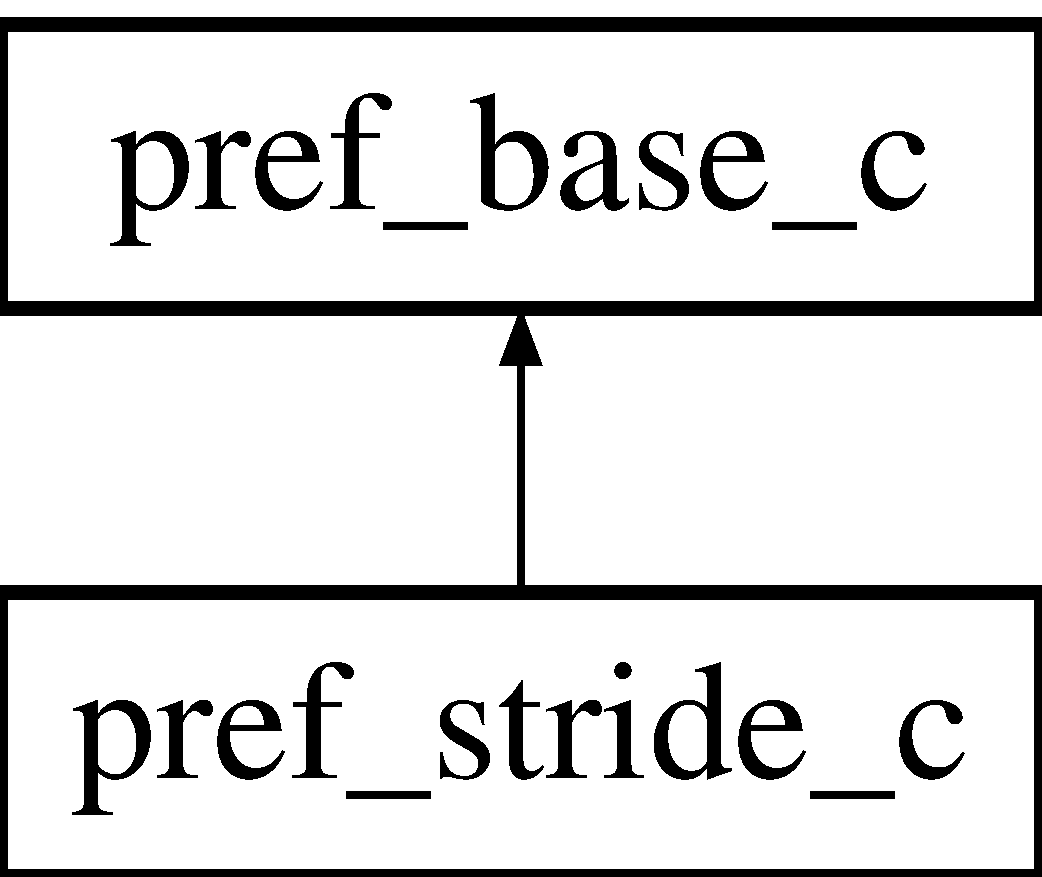
\includegraphics[height=2.000000cm]{classpref__stride__c}
\end{center}
\end{figure}
\subsection*{Public Member Functions}
\begin{DoxyCompactItemize}
\item 
\hyperlink{classpref__stride__c_a0c7831df021d2e585b268dd0605ba852}{pref\_\-stride\_\-c} (\hyperlink{classmacsim__c}{macsim\_\-c} $\ast$simBase)
\item 
\hyperlink{classpref__stride__c_ada308e1e3ce5736adf52e46cd10327dd}{pref\_\-stride\_\-c} (\hyperlink{classhwp__common__c}{hwp\_\-common\_\-c} $\ast$, Unit\_\-Type, \hyperlink{classmacsim__c}{macsim\_\-c} $\ast$simBase)
\item 
\hyperlink{classpref__stride__c_ad5d7b93da62f373b582b79d5ac4bbc25}{$\sim$pref\_\-stride\_\-c} ()
\item 
void \hyperlink{classpref__stride__c_a09ed6d4a95388ec667244be7d977eea2}{init\_\-func} (int)
\item 
void \hyperlink{classpref__stride__c_a147e597a5eb20dc3b903c3c5eaf8973b}{done\_\-func} ()
\item 
void \hyperlink{classpref__stride__c_a7a75dcfa0945e493306b41b7f7d807f6}{l1\_\-miss\_\-func} (int, Addr, Addr, \hyperlink{classuop__c}{uop\_\-c} $\ast$)
\item 
void \hyperlink{classpref__stride__c_a9021353112572858151e53b6c96df0b8}{l1\_\-hit\_\-func} (int, Addr, Addr, \hyperlink{classuop__c}{uop\_\-c} $\ast$)
\item 
void \hyperlink{classpref__stride__c_aeb8654a0fae97b42d1945d2b8f99c795}{l1\_\-pref\_\-hit\_\-func} (int, Addr, Addr, \hyperlink{classuop__c}{uop\_\-c} $\ast$)
\item 
void \hyperlink{classpref__stride__c_a4083ad3dba1bb8357c32f035a464de83}{l2\_\-miss\_\-func} (int, Addr, Addr, \hyperlink{classuop__c}{uop\_\-c} $\ast$)
\item 
void \hyperlink{classpref__stride__c_a7dfd002eebf50de73efe93b53c033044}{l2\_\-hit\_\-func} (int, Addr, Addr, \hyperlink{classuop__c}{uop\_\-c} $\ast$)
\item 
void \hyperlink{classpref__stride__c_acbaa296a61779db50bc2ff8b3807b434}{l2\_\-pref\_\-hit\_\-func} (int, Addr, Addr, \hyperlink{classuop__c}{uop\_\-c} $\ast$)
\item 
void \hyperlink{classpref__stride__c_a948578da09667bbb0ab8eade1a81780d}{train} (int, Addr, Addr, bool)
\item 
void \hyperlink{classpref__stride__c_a25bde09673728625928bb4c2bd5c2eaf}{create\_\-newentry} (int idx, Addr line\_\-addr, Addr region\_\-tag)
\end{DoxyCompactItemize}
\subsection*{Private Attributes}
\begin{DoxyCompactItemize}
\item 
\hyperlink{structstride__region__table__entry__struct}{stride\_\-region\_\-table\_\-entry\_\-s} $\ast$ \hyperlink{classpref__stride__c_a55067688237bc3ef1daf46fda528e38a}{region\_\-table}
\item 
\hyperlink{structstride__index__table__entry__struct}{stride\_\-index\_\-table\_\-entry\_\-s} $\ast$ \hyperlink{classpref__stride__c_af353e647ce9b0007baa0c35f55ec2e05}{index\_\-table}
\end{DoxyCompactItemize}
\subsection*{Friends}
\begin{DoxyCompactItemize}
\item 
\hypertarget{classpref__stride__c_a8d09d4836ddc352da5be834d4969b647}{
class {\bfseries pref\_\-common\_\-c}}
\label{classpref__stride__c_a8d09d4836ddc352da5be834d4969b647}

\end{DoxyCompactItemize}


\subsection{Detailed Description}
stride prefetcher Stride prefetcher. For more detailed information, refer to \hyperlink{classpref__base__c}{pref\_\-base\_\-c} class \begin{DoxySeeAlso}{See also}
\hyperlink{classpref__base__c}{pref\_\-base\_\-c} 
\end{DoxySeeAlso}


\subsection{Constructor \& Destructor Documentation}
\hypertarget{classpref__stride__c_a0c7831df021d2e585b268dd0605ba852}{
\index{pref\_\-stride\_\-c@{pref\_\-stride\_\-c}!pref\_\-stride\_\-c@{pref\_\-stride\_\-c}}
\index{pref\_\-stride\_\-c@{pref\_\-stride\_\-c}!pref_stride_c@{pref\_\-stride\_\-c}}
\subsubsection[{pref\_\-stride\_\-c}]{\setlength{\rightskip}{0pt plus 5cm}pref\_\-stride\_\-c::pref\_\-stride\_\-c (
\begin{DoxyParamCaption}
\item[{{\bf macsim\_\-c} $\ast$}]{ simBase}
\end{DoxyParamCaption}
)}}
\label{classpref__stride__c_a0c7831df021d2e585b268dd0605ba852}
Default constructor \hypertarget{classpref__stride__c_ada308e1e3ce5736adf52e46cd10327dd}{
\index{pref\_\-stride\_\-c@{pref\_\-stride\_\-c}!pref\_\-stride\_\-c@{pref\_\-stride\_\-c}}
\index{pref\_\-stride\_\-c@{pref\_\-stride\_\-c}!pref_stride_c@{pref\_\-stride\_\-c}}
\subsubsection[{pref\_\-stride\_\-c}]{\setlength{\rightskip}{0pt plus 5cm}pref\_\-stride\_\-c::pref\_\-stride\_\-c (
\begin{DoxyParamCaption}
\item[{{\bf hwp\_\-common\_\-c} $\ast$}]{ hcc, }
\item[{Unit\_\-Type}]{ type, }
\item[{{\bf macsim\_\-c} $\ast$}]{ simBase}
\end{DoxyParamCaption}
)}}
\label{classpref__stride__c_ada308e1e3ce5736adf52e46cd10327dd}
Constructor \hypertarget{classpref__stride__c_ad5d7b93da62f373b582b79d5ac4bbc25}{
\index{pref\_\-stride\_\-c@{pref\_\-stride\_\-c}!$\sim$pref\_\-stride\_\-c@{$\sim$pref\_\-stride\_\-c}}
\index{$\sim$pref\_\-stride\_\-c@{$\sim$pref\_\-stride\_\-c}!pref_stride_c@{pref\_\-stride\_\-c}}
\subsubsection[{$\sim$pref\_\-stride\_\-c}]{\setlength{\rightskip}{0pt plus 5cm}pref\_\-stride\_\-c::$\sim$pref\_\-stride\_\-c (
\begin{DoxyParamCaption}
{}
\end{DoxyParamCaption}
)}}
\label{classpref__stride__c_ad5d7b93da62f373b582b79d5ac4bbc25}
Destructor 

\subsection{Member Function Documentation}
\hypertarget{classpref__stride__c_a25bde09673728625928bb4c2bd5c2eaf}{
\index{pref\_\-stride\_\-c@{pref\_\-stride\_\-c}!create\_\-newentry@{create\_\-newentry}}
\index{create\_\-newentry@{create\_\-newentry}!pref_stride_c@{pref\_\-stride\_\-c}}
\subsubsection[{create\_\-newentry}]{\setlength{\rightskip}{0pt plus 5cm}void pref\_\-stride\_\-c::create\_\-newentry (
\begin{DoxyParamCaption}
\item[{int}]{ idx, }
\item[{Addr}]{ line\_\-addr, }
\item[{Addr}]{ region\_\-tag}
\end{DoxyParamCaption}
)}}
\label{classpref__stride__c_a25bde09673728625928bb4c2bd5c2eaf}
Create a new stride \hypertarget{classpref__stride__c_a147e597a5eb20dc3b903c3c5eaf8973b}{
\index{pref\_\-stride\_\-c@{pref\_\-stride\_\-c}!done\_\-func@{done\_\-func}}
\index{done\_\-func@{done\_\-func}!pref_stride_c@{pref\_\-stride\_\-c}}
\subsubsection[{done\_\-func}]{\setlength{\rightskip}{0pt plus 5cm}void pref\_\-stride\_\-c::done\_\-func (
\begin{DoxyParamCaption}
{}
\end{DoxyParamCaption}
)\hspace{0.3cm}{\ttfamily  \mbox{[}inline, virtual\mbox{]}}}}
\label{classpref__stride__c_a147e597a5eb20dc3b903c3c5eaf8973b}
Done function 

Implements \hyperlink{classpref__base__c_af6f4f755ba7bc869f5bae908969eb969}{pref\_\-base\_\-c}.

\hypertarget{classpref__stride__c_a09ed6d4a95388ec667244be7d977eea2}{
\index{pref\_\-stride\_\-c@{pref\_\-stride\_\-c}!init\_\-func@{init\_\-func}}
\index{init\_\-func@{init\_\-func}!pref_stride_c@{pref\_\-stride\_\-c}}
\subsubsection[{init\_\-func}]{\setlength{\rightskip}{0pt plus 5cm}void pref\_\-stride\_\-c::init\_\-func (
\begin{DoxyParamCaption}
\item[{int}]{ core\_\-id}
\end{DoxyParamCaption}
)\hspace{0.3cm}{\ttfamily  \mbox{[}virtual\mbox{]}}}}
\label{classpref__stride__c_a09ed6d4a95388ec667244be7d977eea2}
Init function 

Implements \hyperlink{classpref__base__c_a404371f4c7e814352f3a6e0a1aeb4a9b}{pref\_\-base\_\-c}.

\hypertarget{classpref__stride__c_a9021353112572858151e53b6c96df0b8}{
\index{pref\_\-stride\_\-c@{pref\_\-stride\_\-c}!l1\_\-hit\_\-func@{l1\_\-hit\_\-func}}
\index{l1\_\-hit\_\-func@{l1\_\-hit\_\-func}!pref_stride_c@{pref\_\-stride\_\-c}}
\subsubsection[{l1\_\-hit\_\-func}]{\setlength{\rightskip}{0pt plus 5cm}void pref\_\-stride\_\-c::l1\_\-hit\_\-func (
\begin{DoxyParamCaption}
\item[{int}]{ tid, }
\item[{Addr}]{ lineAddr, }
\item[{Addr}]{ loadPC, }
\item[{{\bf uop\_\-c} $\ast$}]{ uop}
\end{DoxyParamCaption}
)\hspace{0.3cm}{\ttfamily  \mbox{[}virtual\mbox{]}}}}
\label{classpref__stride__c_a9021353112572858151e53b6c96df0b8}
L1 hit function 

Implements \hyperlink{classpref__base__c_a39c3f0b35e3346133be50dbef1b5aa13}{pref\_\-base\_\-c}.

\hypertarget{classpref__stride__c_a7a75dcfa0945e493306b41b7f7d807f6}{
\index{pref\_\-stride\_\-c@{pref\_\-stride\_\-c}!l1\_\-miss\_\-func@{l1\_\-miss\_\-func}}
\index{l1\_\-miss\_\-func@{l1\_\-miss\_\-func}!pref_stride_c@{pref\_\-stride\_\-c}}
\subsubsection[{l1\_\-miss\_\-func}]{\setlength{\rightskip}{0pt plus 5cm}void pref\_\-stride\_\-c::l1\_\-miss\_\-func (
\begin{DoxyParamCaption}
\item[{int}]{ tid, }
\item[{Addr}]{ lineAddr, }
\item[{Addr}]{ loadPC, }
\item[{{\bf uop\_\-c} $\ast$}]{ uop}
\end{DoxyParamCaption}
)\hspace{0.3cm}{\ttfamily  \mbox{[}virtual\mbox{]}}}}
\label{classpref__stride__c_a7a75dcfa0945e493306b41b7f7d807f6}
L1 miss function 

Implements \hyperlink{classpref__base__c_a2b23d47a615b8bb700bd79104bcc1855}{pref\_\-base\_\-c}.

\hypertarget{classpref__stride__c_aeb8654a0fae97b42d1945d2b8f99c795}{
\index{pref\_\-stride\_\-c@{pref\_\-stride\_\-c}!l1\_\-pref\_\-hit\_\-func@{l1\_\-pref\_\-hit\_\-func}}
\index{l1\_\-pref\_\-hit\_\-func@{l1\_\-pref\_\-hit\_\-func}!pref_stride_c@{pref\_\-stride\_\-c}}
\subsubsection[{l1\_\-pref\_\-hit\_\-func}]{\setlength{\rightskip}{0pt plus 5cm}void pref\_\-stride\_\-c::l1\_\-pref\_\-hit\_\-func (
\begin{DoxyParamCaption}
\item[{int}]{, }
\item[{Addr}]{, }
\item[{Addr}]{, }
\item[{{\bf uop\_\-c} $\ast$}]{}
\end{DoxyParamCaption}
)\hspace{0.3cm}{\ttfamily  \mbox{[}inline, virtual\mbox{]}}}}
\label{classpref__stride__c_aeb8654a0fae97b42d1945d2b8f99c795}
L1 prefetch hit function 

Implements \hyperlink{classpref__base__c_a0d54d273c63a4c78873632b6ae1953a7}{pref\_\-base\_\-c}.

\hypertarget{classpref__stride__c_a7dfd002eebf50de73efe93b53c033044}{
\index{pref\_\-stride\_\-c@{pref\_\-stride\_\-c}!l2\_\-hit\_\-func@{l2\_\-hit\_\-func}}
\index{l2\_\-hit\_\-func@{l2\_\-hit\_\-func}!pref_stride_c@{pref\_\-stride\_\-c}}
\subsubsection[{l2\_\-hit\_\-func}]{\setlength{\rightskip}{0pt plus 5cm}void pref\_\-stride\_\-c::l2\_\-hit\_\-func (
\begin{DoxyParamCaption}
\item[{int}]{ tid, }
\item[{Addr}]{ lineAddr, }
\item[{Addr}]{ loadPC, }
\item[{{\bf uop\_\-c} $\ast$}]{ uop}
\end{DoxyParamCaption}
)\hspace{0.3cm}{\ttfamily  \mbox{[}virtual\mbox{]}}}}
\label{classpref__stride__c_a7dfd002eebf50de73efe93b53c033044}
L2 hit function 

Implements \hyperlink{classpref__base__c_acba9e1586edcddff8983b46c2147e80d}{pref\_\-base\_\-c}.

\hypertarget{classpref__stride__c_a4083ad3dba1bb8357c32f035a464de83}{
\index{pref\_\-stride\_\-c@{pref\_\-stride\_\-c}!l2\_\-miss\_\-func@{l2\_\-miss\_\-func}}
\index{l2\_\-miss\_\-func@{l2\_\-miss\_\-func}!pref_stride_c@{pref\_\-stride\_\-c}}
\subsubsection[{l2\_\-miss\_\-func}]{\setlength{\rightskip}{0pt plus 5cm}void pref\_\-stride\_\-c::l2\_\-miss\_\-func (
\begin{DoxyParamCaption}
\item[{int}]{ tid, }
\item[{Addr}]{ lineAddr, }
\item[{Addr}]{ loadPC, }
\item[{{\bf uop\_\-c} $\ast$}]{ uop}
\end{DoxyParamCaption}
)\hspace{0.3cm}{\ttfamily  \mbox{[}virtual\mbox{]}}}}
\label{classpref__stride__c_a4083ad3dba1bb8357c32f035a464de83}
L2 miss function 

Implements \hyperlink{classpref__base__c_afe9bb0f31178fc9acf2d35afe65d6cd0}{pref\_\-base\_\-c}.

\hypertarget{classpref__stride__c_acbaa296a61779db50bc2ff8b3807b434}{
\index{pref\_\-stride\_\-c@{pref\_\-stride\_\-c}!l2\_\-pref\_\-hit\_\-func@{l2\_\-pref\_\-hit\_\-func}}
\index{l2\_\-pref\_\-hit\_\-func@{l2\_\-pref\_\-hit\_\-func}!pref_stride_c@{pref\_\-stride\_\-c}}
\subsubsection[{l2\_\-pref\_\-hit\_\-func}]{\setlength{\rightskip}{0pt plus 5cm}void pref\_\-stride\_\-c::l2\_\-pref\_\-hit\_\-func (
\begin{DoxyParamCaption}
\item[{int}]{, }
\item[{Addr}]{, }
\item[{Addr}]{, }
\item[{{\bf uop\_\-c} $\ast$}]{}
\end{DoxyParamCaption}
)\hspace{0.3cm}{\ttfamily  \mbox{[}inline, virtual\mbox{]}}}}
\label{classpref__stride__c_acbaa296a61779db50bc2ff8b3807b434}
L2 prefetch hit function 

Implements \hyperlink{classpref__base__c_ae89bc30a1f74a1199bec721ca78197c1}{pref\_\-base\_\-c}.

\hypertarget{classpref__stride__c_a948578da09667bbb0ab8eade1a81780d}{
\index{pref\_\-stride\_\-c@{pref\_\-stride\_\-c}!train@{train}}
\index{train@{train}!pref_stride_c@{pref\_\-stride\_\-c}}
\subsubsection[{train}]{\setlength{\rightskip}{0pt plus 5cm}void pref\_\-stride\_\-c::train (
\begin{DoxyParamCaption}
\item[{int}]{ tid, }
\item[{Addr}]{ lineAddr, }
\item[{Addr}]{ loadPC, }
\item[{bool}]{ l2\_\-hit}
\end{DoxyParamCaption}
)}}
\label{classpref__stride__c_a948578da09667bbb0ab8eade1a81780d}
Train stride table 

\subsection{Member Data Documentation}
\hypertarget{classpref__stride__c_af353e647ce9b0007baa0c35f55ec2e05}{
\index{pref\_\-stride\_\-c@{pref\_\-stride\_\-c}!index\_\-table@{index\_\-table}}
\index{index\_\-table@{index\_\-table}!pref_stride_c@{pref\_\-stride\_\-c}}
\subsubsection[{index\_\-table}]{\setlength{\rightskip}{0pt plus 5cm}{\bf stride\_\-index\_\-table\_\-entry\_\-s}$\ast$ {\bf pref\_\-stride\_\-c::index\_\-table}\hspace{0.3cm}{\ttfamily  \mbox{[}private\mbox{]}}}}
\label{classpref__stride__c_af353e647ce9b0007baa0c35f55ec2e05}
prefetch table \hypertarget{classpref__stride__c_a55067688237bc3ef1daf46fda528e38a}{
\index{pref\_\-stride\_\-c@{pref\_\-stride\_\-c}!region\_\-table@{region\_\-table}}
\index{region\_\-table@{region\_\-table}!pref_stride_c@{pref\_\-stride\_\-c}}
\subsubsection[{region\_\-table}]{\setlength{\rightskip}{0pt plus 5cm}{\bf stride\_\-region\_\-table\_\-entry\_\-s}$\ast$ {\bf pref\_\-stride\_\-c::region\_\-table}\hspace{0.3cm}{\ttfamily  \mbox{[}private\mbox{]}}}}
\label{classpref__stride__c_a55067688237bc3ef1daf46fda528e38a}
address region info 

The documentation for this class was generated from the following files:\begin{DoxyCompactItemize}
\item 
pref\_\-stride.h\item 
pref\_\-stride.cc\end{DoxyCompactItemize}

\hypertarget{classprocess__manager__c}{
\section{process\_\-manager\_\-c Class Reference}
\label{classprocess__manager__c}\index{process\_\-manager\_\-c@{process\_\-manager\_\-c}}
}


Process and Thread manager class.  




{\ttfamily \#include $<$process\_\-manager.h$>$}

\subsection*{Public Member Functions}
\begin{DoxyCompactItemize}
\item 
\hyperlink{classprocess__manager__c_acd81384cecb912bd143ec14ef1b74f95}{process\_\-manager\_\-c} (\hyperlink{classmacsim__c}{macsim\_\-c} $\ast$simBase)
\item 
\hyperlink{classprocess__manager__c_a9c459d11d9290dc96e40224eb12e51ca}{$\sim$process\_\-manager\_\-c} ()
\item 
int \hyperlink{classprocess__manager__c_aae08e9591cbeac5e916852bcd43b5708}{create\_\-process} (string appl)
\item 
int \hyperlink{classprocess__manager__c_af9c5bd91b7afdb6c53371b0228fb29b7}{create\_\-process} (string appl, int repeat, int pid)
\item 
bool \hyperlink{classprocess__manager__c_a4706b28e0c7b73c49fdc89596bca8308}{terminate\_\-process} (\hyperlink{structprocess__s}{process\_\-s} $\ast$process)
\item 
void \hyperlink{classprocess__manager__c_afe1750e1d8e076cd2efb1b62fcde1276}{setup\_\-process} (\hyperlink{structprocess__s}{process\_\-s} $\ast$process)
\item 
void \hyperlink{classprocess__manager__c_a27441c6e84b6d582d375a3670b4823df}{create\_\-thread\_\-node} (\hyperlink{structprocess__s}{process\_\-s} $\ast$process, int tid, bool main)
\item 
int \hyperlink{classprocess__manager__c_a71be3931ab2a657faf979f0a0fc719a6}{terminate\_\-thread} (int core\_\-id, \hyperlink{structthread__s}{thread\_\-s} $\ast$trace\_\-info, int thread\_\-id, int block\_\-id)
\item 
void \hyperlink{classprocess__manager__c_af6aa8eb4d2257fc6e0f6c054e298fad4}{sim\_\-thread\_\-schedule} (void)
\end{DoxyCompactItemize}
\subsection*{Private Member Functions}
\begin{DoxyCompactItemize}
\item 
int \hyperlink{classprocess__manager__c_af5b771accff1a1a586eda0fff5d731c4}{sim\_\-schedule\_\-thread\_\-block} (int core\_\-id)
\item 
void \hyperlink{classprocess__manager__c_aac295c0fb13eee3ac88eb194f6490d38}{insert\_\-thread} (\hyperlink{structthread__trace__info__node__s}{thread\_\-trace\_\-info\_\-node\_\-s} $\ast$incoming)
\item 
void \hyperlink{classprocess__manager__c_a5fa5c35eb19fd242cd6f6f10ff5e5d59}{insert\_\-block} (\hyperlink{structthread__trace__info__node__s}{thread\_\-trace\_\-info\_\-node\_\-s} $\ast$incoming)
\item 
\hyperlink{structthread__trace__info__node__s}{thread\_\-trace\_\-info\_\-node\_\-s} $\ast$ \hyperlink{classprocess__manager__c_ade9cab5331bac2126425b1152d3e7163}{fetch\_\-thread} ()
\item 
\hyperlink{structthread__trace__info__node__s}{thread\_\-trace\_\-info\_\-node\_\-s} $\ast$ \hyperlink{classprocess__manager__c_a7c24e875698b8dd7da47597a5b2fb2aa}{fetch\_\-block} (int block\_\-id)
\item 
\hyperlink{structthread__s}{thread\_\-s} $\ast$ \hyperlink{classprocess__manager__c_ab37b9bf4f76080b5a6adb5e902a761ef}{create\_\-thread} (\hyperlink{structprocess__s}{process\_\-s} $\ast$process, int tid, bool main)
\end{DoxyCompactItemize}
\subsection*{Private Attributes}
\begin{DoxyCompactItemize}
\item 
list$<$ \hyperlink{structthread__trace__info__node__s}{thread\_\-trace\_\-info\_\-node\_\-s} $\ast$ $>$ $\ast$ \hyperlink{classprocess__manager__c_a0fa9dc97ed1a88aadc63b0a82ef24896}{m\_\-thread\_\-queue}
\item 
unordered\_\-map$<$ int, list$<$ \hyperlink{structthread__trace__info__node__s}{thread\_\-trace\_\-info\_\-node\_\-s} $\ast$ $>$ $\ast$ $>$ $\ast$ \hyperlink{classprocess__manager__c_a07f5bef183ba3a7f15ed362c562c1137}{m\_\-block\_\-queue}
\item 
\hyperlink{classpool__c}{pool\_\-c}$<$ \hyperlink{classhash__c}{hash\_\-c}$<$ \hyperlink{classinst__info__s}{inst\_\-info\_\-s} $>$ $>$ $\ast$ \hyperlink{classprocess__manager__c_ae5ef36e1434826d79d370c9afcb174bc}{m\_\-inst\_\-hash\_\-pool}
\item 
\hypertarget{classprocess__manager__c_a556db8ba188f7831fdae0c7b608cf731}{
unordered\_\-map$<$ int, Counter $>$ {\bfseries m\_\-appl\_\-cyccount\_\-info}}
\label{classprocess__manager__c_a556db8ba188f7831fdae0c7b608cf731}

\item 
\hyperlink{classmacsim__c}{macsim\_\-c} $\ast$ \hyperlink{classprocess__manager__c_a6cca65c36ed2b7747dd13857fcce6ee9}{m\_\-simBase}
\end{DoxyCompactItemize}


\subsection{Detailed Description}
Process and Thread manager class. Schedule processes and threads for the simulation. 

\subsection{Constructor \& Destructor Documentation}
\hypertarget{classprocess__manager__c_acd81384cecb912bd143ec14ef1b74f95}{
\index{process\_\-manager\_\-c@{process\_\-manager\_\-c}!process\_\-manager\_\-c@{process\_\-manager\_\-c}}
\index{process\_\-manager\_\-c@{process\_\-manager\_\-c}!process_manager_c@{process\_\-manager\_\-c}}
\subsubsection[{process\_\-manager\_\-c}]{\setlength{\rightskip}{0pt plus 5cm}process\_\-manager\_\-c::process\_\-manager\_\-c (
\begin{DoxyParamCaption}
\item[{{\bf macsim\_\-c} $\ast$}]{ simBase}
\end{DoxyParamCaption}
)}}
\label{classprocess__manager__c_acd81384cecb912bd143ec14ef1b74f95}
Constructor \hypertarget{classprocess__manager__c_a9c459d11d9290dc96e40224eb12e51ca}{
\index{process\_\-manager\_\-c@{process\_\-manager\_\-c}!$\sim$process\_\-manager\_\-c@{$\sim$process\_\-manager\_\-c}}
\index{$\sim$process\_\-manager\_\-c@{$\sim$process\_\-manager\_\-c}!process_manager_c@{process\_\-manager\_\-c}}
\subsubsection[{$\sim$process\_\-manager\_\-c}]{\setlength{\rightskip}{0pt plus 5cm}process\_\-manager\_\-c::$\sim$process\_\-manager\_\-c (
\begin{DoxyParamCaption}
{}
\end{DoxyParamCaption}
)}}
\label{classprocess__manager__c_a9c459d11d9290dc96e40224eb12e51ca}
Destructor 

\subsection{Member Function Documentation}
\hypertarget{classprocess__manager__c_aae08e9591cbeac5e916852bcd43b5708}{
\index{process\_\-manager\_\-c@{process\_\-manager\_\-c}!create\_\-process@{create\_\-process}}
\index{create\_\-process@{create\_\-process}!process_manager_c@{process\_\-manager\_\-c}}
\subsubsection[{create\_\-process}]{\setlength{\rightskip}{0pt plus 5cm}int process\_\-manager\_\-c::create\_\-process (
\begin{DoxyParamCaption}
\item[{string}]{ appl}
\end{DoxyParamCaption}
)}}
\label{classprocess__manager__c_aae08e9591cbeac5e916852bcd43b5708}
Create a new process. 
\begin{DoxyParams}{Parameters}
\item[{\em appl}]application path \end{DoxyParams}
\hypertarget{classprocess__manager__c_af9c5bd91b7afdb6c53371b0228fb29b7}{
\index{process\_\-manager\_\-c@{process\_\-manager\_\-c}!create\_\-process@{create\_\-process}}
\index{create\_\-process@{create\_\-process}!process_manager_c@{process\_\-manager\_\-c}}
\subsubsection[{create\_\-process}]{\setlength{\rightskip}{0pt plus 5cm}int process\_\-manager\_\-c::create\_\-process (
\begin{DoxyParamCaption}
\item[{string}]{ appl, }
\item[{int}]{ repeat, }
\item[{int}]{ pid}
\end{DoxyParamCaption}
)}}
\label{classprocess__manager__c_af9c5bd91b7afdb6c53371b0228fb29b7}
Create a new process. 
\begin{DoxyParams}{Parameters}
\item[{\em appl}]application path \item[{\em repeat}]whether this process has been re-\/executed. When we run multiple programs workloads, we may need to repeat terminated applications. \item[{\em pid}]original process id \end{DoxyParams}


Create a process and setup id and other fields

Get configurations from the file

\hypertarget{classprocess__manager__c_ab37b9bf4f76080b5a6adb5e902a761ef}{
\index{process\_\-manager\_\-c@{process\_\-manager\_\-c}!create\_\-thread@{create\_\-thread}}
\index{create\_\-thread@{create\_\-thread}!process_manager_c@{process\_\-manager\_\-c}}
\subsubsection[{create\_\-thread}]{\setlength{\rightskip}{0pt plus 5cm}{\bf thread\_\-s} $\ast$ process\_\-manager\_\-c::create\_\-thread (
\begin{DoxyParamCaption}
\item[{{\bf process\_\-s} $\ast$}]{ process, }
\item[{int}]{ tid, }
\item[{bool}]{ main}
\end{DoxyParamCaption}
)\hspace{0.3cm}{\ttfamily  \mbox{[}private\mbox{]}}}}
\label{classprocess__manager__c_ab37b9bf4f76080b5a6adb5e902a761ef}
Create a new thread. A thread has been created when create\_\-thread\_\-node has been called. However, when a thread is actually scheduled, memory allocation and initialization will be performed. 
\begin{DoxyParams}{Parameters}
\item[{\em process}]-\/ process \item[{\em tid}]-\/ thread id \item[{\em main}]-\/ indicate main thread (usually thread id 0) \end{DoxyParams}
\hypertarget{classprocess__manager__c_a27441c6e84b6d582d375a3670b4823df}{
\index{process\_\-manager\_\-c@{process\_\-manager\_\-c}!create\_\-thread\_\-node@{create\_\-thread\_\-node}}
\index{create\_\-thread\_\-node@{create\_\-thread\_\-node}!process_manager_c@{process\_\-manager\_\-c}}
\subsubsection[{create\_\-thread\_\-node}]{\setlength{\rightskip}{0pt plus 5cm}void process\_\-manager\_\-c::create\_\-thread\_\-node (
\begin{DoxyParamCaption}
\item[{{\bf process\_\-s} $\ast$}]{ process, }
\item[{int}]{ tid, }
\item[{bool}]{ main}
\end{DoxyParamCaption}
)}}
\label{classprocess__manager__c_a27441c6e84b6d582d375a3670b4823df}
Create a thread node. In scheduler, a node will be inserted or deleted. When a node is scheduled, all memory allocation and other initializations will be performed. 
\begin{DoxyParams}{Parameters}
\item[{\em process}]process \item[{\em tid}]thread id \item[{\em main}]When set, indicate master thread (usually thread 0) \end{DoxyParams}
\hypertarget{classprocess__manager__c_a7c24e875698b8dd7da47597a5b2fb2aa}{
\index{process\_\-manager\_\-c@{process\_\-manager\_\-c}!fetch\_\-block@{fetch\_\-block}}
\index{fetch\_\-block@{fetch\_\-block}!process_manager_c@{process\_\-manager\_\-c}}
\subsubsection[{fetch\_\-block}]{\setlength{\rightskip}{0pt plus 5cm}{\bf thread\_\-trace\_\-info\_\-node\_\-s} $\ast$ process\_\-manager\_\-c::fetch\_\-block (
\begin{DoxyParamCaption}
\item[{int}]{ block\_\-id}
\end{DoxyParamCaption}
)\hspace{0.3cm}{\ttfamily  \mbox{[}private\mbox{]}}}}
\label{classprocess__manager__c_a7c24e875698b8dd7da47597a5b2fb2aa}
Fetch a new thread from the block which is in the front of block scheduling queue \hypertarget{classprocess__manager__c_ade9cab5331bac2126425b1152d3e7163}{
\index{process\_\-manager\_\-c@{process\_\-manager\_\-c}!fetch\_\-thread@{fetch\_\-thread}}
\index{fetch\_\-thread@{fetch\_\-thread}!process_manager_c@{process\_\-manager\_\-c}}
\subsubsection[{fetch\_\-thread}]{\setlength{\rightskip}{0pt plus 5cm}{\bf thread\_\-trace\_\-info\_\-node\_\-s} $\ast$ process\_\-manager\_\-c::fetch\_\-thread (
\begin{DoxyParamCaption}
\item[{void}]{}
\end{DoxyParamCaption}
)\hspace{0.3cm}{\ttfamily  \mbox{[}private\mbox{]}}}}
\label{classprocess__manager__c_ade9cab5331bac2126425b1152d3e7163}
Fetch a new thread which is in the front of scheduling queue \hypertarget{classprocess__manager__c_a5fa5c35eb19fd242cd6f6f10ff5e5d59}{
\index{process\_\-manager\_\-c@{process\_\-manager\_\-c}!insert\_\-block@{insert\_\-block}}
\index{insert\_\-block@{insert\_\-block}!process_manager_c@{process\_\-manager\_\-c}}
\subsubsection[{insert\_\-block}]{\setlength{\rightskip}{0pt plus 5cm}void process\_\-manager\_\-c::insert\_\-block (
\begin{DoxyParamCaption}
\item[{{\bf thread\_\-trace\_\-info\_\-node\_\-s} $\ast$}]{ incoming}
\end{DoxyParamCaption}
)\hspace{0.3cm}{\ttfamily  \mbox{[}private\mbox{]}}}}
\label{classprocess__manager__c_a5fa5c35eb19fd242cd6f6f10ff5e5d59}
Insert a new thread to the block scheduler 
\begin{DoxyParams}{Parameters}
\item[{\em incoming}]-\/ a new thread \end{DoxyParams}
\hypertarget{classprocess__manager__c_aac295c0fb13eee3ac88eb194f6490d38}{
\index{process\_\-manager\_\-c@{process\_\-manager\_\-c}!insert\_\-thread@{insert\_\-thread}}
\index{insert\_\-thread@{insert\_\-thread}!process_manager_c@{process\_\-manager\_\-c}}
\subsubsection[{insert\_\-thread}]{\setlength{\rightskip}{0pt plus 5cm}void process\_\-manager\_\-c::insert\_\-thread (
\begin{DoxyParamCaption}
\item[{{\bf thread\_\-trace\_\-info\_\-node\_\-s} $\ast$}]{ incoming}
\end{DoxyParamCaption}
)\hspace{0.3cm}{\ttfamily  \mbox{[}private\mbox{]}}}}
\label{classprocess__manager__c_aac295c0fb13eee3ac88eb194f6490d38}
Insert a new thread to the scheduler 
\begin{DoxyParams}{Parameters}
\item[{\em incoming}]-\/ a new thread \end{DoxyParams}
\hypertarget{classprocess__manager__c_afe1750e1d8e076cd2efb1b62fcde1276}{
\index{process\_\-manager\_\-c@{process\_\-manager\_\-c}!setup\_\-process@{setup\_\-process}}
\index{setup\_\-process@{setup\_\-process}!process_manager_c@{process\_\-manager\_\-c}}
\subsubsection[{setup\_\-process}]{\setlength{\rightskip}{0pt plus 5cm}void process\_\-manager\_\-c::setup\_\-process (
\begin{DoxyParamCaption}
\item[{{\bf process\_\-s} $\ast$}]{ process}
\end{DoxyParamCaption}
)}}
\label{classprocess__manager__c_afe1750e1d8e076cd2efb1b62fcde1276}
Setup a process (data structure, initialization ..) \hypertarget{classprocess__manager__c_af5b771accff1a1a586eda0fff5d731c4}{
\index{process\_\-manager\_\-c@{process\_\-manager\_\-c}!sim\_\-schedule\_\-thread\_\-block@{sim\_\-schedule\_\-thread\_\-block}}
\index{sim\_\-schedule\_\-thread\_\-block@{sim\_\-schedule\_\-thread\_\-block}!process_manager_c@{process\_\-manager\_\-c}}
\subsubsection[{sim\_\-schedule\_\-thread\_\-block}]{\setlength{\rightskip}{0pt plus 5cm}int process\_\-manager\_\-c::sim\_\-schedule\_\-thread\_\-block (
\begin{DoxyParamCaption}
\item[{int}]{ core\_\-id}
\end{DoxyParamCaption}
)\hspace{0.3cm}{\ttfamily  \mbox{[}private\mbox{]}}}}
\label{classprocess__manager__c_af5b771accff1a1a586eda0fff5d731c4}
GPU simulation : schedule a thread from a block 
\begin{DoxyParams}{Parameters}
\item[{\em core\_\-id}]-\/ core to schedule a new thread \end{DoxyParams}
\hypertarget{classprocess__manager__c_af6aa8eb4d2257fc6e0f6c054e298fad4}{
\index{process\_\-manager\_\-c@{process\_\-manager\_\-c}!sim\_\-thread\_\-schedule@{sim\_\-thread\_\-schedule}}
\index{sim\_\-thread\_\-schedule@{sim\_\-thread\_\-schedule}!process_manager_c@{process\_\-manager\_\-c}}
\subsubsection[{sim\_\-thread\_\-schedule}]{\setlength{\rightskip}{0pt plus 5cm}void process\_\-manager\_\-c::sim\_\-thread\_\-schedule (
\begin{DoxyParamCaption}
\item[{void}]{}
\end{DoxyParamCaption}
)}}
\label{classprocess__manager__c_af6aa8eb4d2257fc6e0f6c054e298fad4}
Schedule a new thread \hypertarget{classprocess__manager__c_a4706b28e0c7b73c49fdc89596bca8308}{
\index{process\_\-manager\_\-c@{process\_\-manager\_\-c}!terminate\_\-process@{terminate\_\-process}}
\index{terminate\_\-process@{terminate\_\-process}!process_manager_c@{process\_\-manager\_\-c}}
\subsubsection[{terminate\_\-process}]{\setlength{\rightskip}{0pt plus 5cm}bool process\_\-manager\_\-c::terminate\_\-process (
\begin{DoxyParamCaption}
\item[{{\bf process\_\-s} $\ast$}]{ process}
\end{DoxyParamCaption}
)}}
\label{classprocess__manager__c_a4706b28e0c7b73c49fdc89596bca8308}
Terminate a process \hypertarget{classprocess__manager__c_a71be3931ab2a657faf979f0a0fc719a6}{
\index{process\_\-manager\_\-c@{process\_\-manager\_\-c}!terminate\_\-thread@{terminate\_\-thread}}
\index{terminate\_\-thread@{terminate\_\-thread}!process_manager_c@{process\_\-manager\_\-c}}
\subsubsection[{terminate\_\-thread}]{\setlength{\rightskip}{0pt plus 5cm}int process\_\-manager\_\-c::terminate\_\-thread (
\begin{DoxyParamCaption}
\item[{int}]{ core\_\-id, }
\item[{{\bf thread\_\-s} $\ast$}]{ trace\_\-info, }
\item[{int}]{ thread\_\-id, }
\item[{int}]{ block\_\-id}
\end{DoxyParamCaption}
)}}
\label{classprocess__manager__c_a71be3931ab2a657faf979f0a0fc719a6}
Terminate a thread 
\begin{DoxyParams}{Parameters}
\item[{\em core\_\-id}]-\/ core id \item[{\em trace\_\-info}]-\/ thread trace information \item[{\em thread\_\-id}]-\/ thread id \item[{\em block\_\-id}]-\/ block id \end{DoxyParams}


\subsection{Member Data Documentation}
\hypertarget{classprocess__manager__c_a07f5bef183ba3a7f15ed362c562c1137}{
\index{process\_\-manager\_\-c@{process\_\-manager\_\-c}!m\_\-block\_\-queue@{m\_\-block\_\-queue}}
\index{m\_\-block\_\-queue@{m\_\-block\_\-queue}!process_manager_c@{process\_\-manager\_\-c}}
\subsubsection[{m\_\-block\_\-queue}]{\setlength{\rightskip}{0pt plus 5cm}unordered\_\-map$<$int, list$<${\bf thread\_\-trace\_\-info\_\-node\_\-s} $\ast$$>$ $\ast$$>$$\ast$ {\bf process\_\-manager\_\-c::m\_\-block\_\-queue}\hspace{0.3cm}{\ttfamily  \mbox{[}private\mbox{]}}}}
\label{classprocess__manager__c_a07f5bef183ba3a7f15ed362c562c1137}
block queue \hypertarget{classprocess__manager__c_ae5ef36e1434826d79d370c9afcb174bc}{
\index{process\_\-manager\_\-c@{process\_\-manager\_\-c}!m\_\-inst\_\-hash\_\-pool@{m\_\-inst\_\-hash\_\-pool}}
\index{m\_\-inst\_\-hash\_\-pool@{m\_\-inst\_\-hash\_\-pool}!process_manager_c@{process\_\-manager\_\-c}}
\subsubsection[{m\_\-inst\_\-hash\_\-pool}]{\setlength{\rightskip}{0pt plus 5cm}{\bf pool\_\-c}$<${\bf hash\_\-c}$<${\bf inst\_\-info\_\-s}$>$ $>$$\ast$ {\bf process\_\-manager\_\-c::m\_\-inst\_\-hash\_\-pool}\hspace{0.3cm}{\ttfamily  \mbox{[}private\mbox{]}}}}
\label{classprocess__manager__c_ae5ef36e1434826d79d370c9afcb174bc}
instruction hash pool \hypertarget{classprocess__manager__c_a6cca65c36ed2b7747dd13857fcce6ee9}{
\index{process\_\-manager\_\-c@{process\_\-manager\_\-c}!m\_\-simBase@{m\_\-simBase}}
\index{m\_\-simBase@{m\_\-simBase}!process_manager_c@{process\_\-manager\_\-c}}
\subsubsection[{m\_\-simBase}]{\setlength{\rightskip}{0pt plus 5cm}{\bf macsim\_\-c}$\ast$ {\bf process\_\-manager\_\-c::m\_\-simBase}\hspace{0.3cm}{\ttfamily  \mbox{[}private\mbox{]}}}}
\label{classprocess__manager__c_a6cca65c36ed2b7747dd13857fcce6ee9}
\hyperlink{classmacsim__c}{macsim\_\-c} base class for simulation globals \hypertarget{classprocess__manager__c_a0fa9dc97ed1a88aadc63b0a82ef24896}{
\index{process\_\-manager\_\-c@{process\_\-manager\_\-c}!m\_\-thread\_\-queue@{m\_\-thread\_\-queue}}
\index{m\_\-thread\_\-queue@{m\_\-thread\_\-queue}!process_manager_c@{process\_\-manager\_\-c}}
\subsubsection[{m\_\-thread\_\-queue}]{\setlength{\rightskip}{0pt plus 5cm}list$<${\bf thread\_\-trace\_\-info\_\-node\_\-s} $\ast$$>$$\ast$ {\bf process\_\-manager\_\-c::m\_\-thread\_\-queue}\hspace{0.3cm}{\ttfamily  \mbox{[}private\mbox{]}}}}
\label{classprocess__manager__c_a0fa9dc97ed1a88aadc63b0a82ef24896}
thread queue 

The documentation for this class was generated from the following files:\begin{DoxyCompactItemize}
\item 
process\_\-manager.h\item 
process\_\-manager.cc\end{DoxyCompactItemize}

\hypertarget{structprocess__s}{
\section{process\_\-s Struct Reference}
\label{structprocess__s}\index{process\_\-s@{process\_\-s}}
}


Process data structure.  




{\ttfamily \#include $<$process\_\-manager.h$>$}

\subsection*{Public Member Functions}
\begin{DoxyCompactItemize}
\item 
\hyperlink{structprocess__s_a837742357aae46f13f2961950397dd76}{process\_\-s} ()
\item 
\hyperlink{structprocess__s_ab0b2900fe44e2e0f3fe45017b26c8ff0}{$\sim$process\_\-s} ()
\end{DoxyCompactItemize}
\subsection*{Public Attributes}
\begin{DoxyCompactItemize}
\item 
unsigned int \hyperlink{structprocess__s_a177fa7999a4380f87de1d1020972d0d8}{m\_\-process\_\-id}
\item 
int \hyperlink{structprocess__s_af321df6fbc03573f3b665b27b857446e}{m\_\-orig\_\-pid}
\item 
int \hyperlink{structprocess__s_a57fa57ad2c2538de96d40d2908837331}{m\_\-max\_\-block}
\item 
\hyperlink{structthread__start__info__s}{thread\_\-start\_\-info\_\-s} $\ast$ \hyperlink{structprocess__s_a948322a5587615947b1080e04f2c76b8}{m\_\-thread\_\-start\_\-info}
\item 
\hyperlink{structthread__s}{thread\_\-s} $\ast$$\ast$ \hyperlink{structprocess__s_ad7a7f06130499ec66febeab3aa686d5b}{m\_\-thread\_\-trace\_\-info}
\item 
unsigned int \hyperlink{structprocess__s_a0da37eb04b86d5257061ad58c55df5fe}{m\_\-no\_\-of\_\-threads}
\item 
unsigned int \hyperlink{structprocess__s_a56d830c06a9f3a2b1569c9d1894ab6e2}{m\_\-no\_\-of\_\-threads\_\-created}
\item 
unsigned int \hyperlink{structprocess__s_a0debe2b803da90b86dcbd113fa79c5e4}{m\_\-no\_\-of\_\-threads\_\-terminated}
\item 
map$<$ int, bool $>$ \hyperlink{structprocess__s_a407d38bd942dd27e620147ac8af9a0a4}{m\_\-core\_\-list}
\item 
queue$<$ int $>$ $\ast$ \hyperlink{structprocess__s_a12b9ed9259a013ff8126089193c93dc2}{m\_\-core\_\-pool}
\item 
bool \hyperlink{structprocess__s_a4578e18b431979d88d1782a080c0b4ce}{m\_\-ptx}
\item 
int \hyperlink{structprocess__s_a7f5a5304526964f084a24b68b0132d7a}{m\_\-repeat}
\item 
vector$<$ string $>$ \hyperlink{structprocess__s_a3f8f9f073f0fc6dfe9c26078a125613c}{m\_\-applications}
\item 
vector$<$ int $>$ \hyperlink{structprocess__s_ae9086b0940b39f7769ee8c2e9b8dadf9}{m\_\-kernel\_\-block\_\-start\_\-count}
\item 
string \hyperlink{structprocess__s_a5bc754a24b94de3a4b1613290905d249}{m\_\-current\_\-file\_\-name\_\-base}
\item 
string \hyperlink{structprocess__s_ac73aecc7aba4805bf7dac8ac9c55edbc}{m\_\-kernel\_\-config\_\-name}
\item 
int \hyperlink{structprocess__s_ab3a31ad6a2b66f08214d9df8c1572f4b}{m\_\-current\_\-vector\_\-index}
\item 
map$<$ int, bool $>$ \hyperlink{structprocess__s_a42b0cd7d3f544dc9cd7689d5ecc98583}{m\_\-block\_\-list}
\item 
uns64 \hyperlink{structprocess__s_a5af0d84f34d9a81519faaf6475bb2bff}{m\_\-inst\_\-count\_\-tot}
\item 
int \hyperlink{structprocess__s_a746e127b1afbcf751be762e21472374b}{m\_\-block\_\-count}
\end{DoxyCompactItemize}


\subsection{Detailed Description}
Process data structure. structure holding information about an application being simulated Mapping between the trace of one application and simulation process 

\subsection{Constructor \& Destructor Documentation}
\hypertarget{structprocess__s_a837742357aae46f13f2961950397dd76}{
\index{process\_\-s@{process\_\-s}!process\_\-s@{process\_\-s}}
\index{process\_\-s@{process\_\-s}!process_s@{process\_\-s}}
\subsubsection[{process\_\-s}]{\setlength{\rightskip}{0pt plus 5cm}process\_\-s::process\_\-s (
\begin{DoxyParamCaption}
{}
\end{DoxyParamCaption}
)}}
\label{structprocess__s_a837742357aae46f13f2961950397dd76}
Constructor \hypertarget{structprocess__s_ab0b2900fe44e2e0f3fe45017b26c8ff0}{
\index{process\_\-s@{process\_\-s}!$\sim$process\_\-s@{$\sim$process\_\-s}}
\index{$\sim$process\_\-s@{$\sim$process\_\-s}!process_s@{process\_\-s}}
\subsubsection[{$\sim$process\_\-s}]{\setlength{\rightskip}{0pt plus 5cm}process\_\-s::$\sim$process\_\-s (
\begin{DoxyParamCaption}
{}
\end{DoxyParamCaption}
)}}
\label{structprocess__s_ab0b2900fe44e2e0f3fe45017b26c8ff0}
Destructor 

\subsection{Member Data Documentation}
\hypertarget{structprocess__s_a3f8f9f073f0fc6dfe9c26078a125613c}{
\index{process\_\-s@{process\_\-s}!m\_\-applications@{m\_\-applications}}
\index{m\_\-applications@{m\_\-applications}!process_s@{process\_\-s}}
\subsubsection[{m\_\-applications}]{\setlength{\rightskip}{0pt plus 5cm}vector$<$string$>$ {\bf process\_\-s::m\_\-applications}}}
\label{structprocess__s_a3f8f9f073f0fc6dfe9c26078a125613c}
list of sub-\/applications \hypertarget{structprocess__s_a746e127b1afbcf751be762e21472374b}{
\index{process\_\-s@{process\_\-s}!m\_\-block\_\-count@{m\_\-block\_\-count}}
\index{m\_\-block\_\-count@{m\_\-block\_\-count}!process_s@{process\_\-s}}
\subsubsection[{m\_\-block\_\-count}]{\setlength{\rightskip}{0pt plus 5cm}int {\bf process\_\-s::m\_\-block\_\-count}}}
\label{structprocess__s_a746e127b1afbcf751be762e21472374b}
total block counts \hypertarget{structprocess__s_a42b0cd7d3f544dc9cd7689d5ecc98583}{
\index{process\_\-s@{process\_\-s}!m\_\-block\_\-list@{m\_\-block\_\-list}}
\index{m\_\-block\_\-list@{m\_\-block\_\-list}!process_s@{process\_\-s}}
\subsubsection[{m\_\-block\_\-list}]{\setlength{\rightskip}{0pt plus 5cm}map$<$int, bool$>$ {\bf process\_\-s::m\_\-block\_\-list}}}
\label{structprocess__s_a42b0cd7d3f544dc9cd7689d5ecc98583}
list of block currently running \hypertarget{structprocess__s_a407d38bd942dd27e620147ac8af9a0a4}{
\index{process\_\-s@{process\_\-s}!m\_\-core\_\-list@{m\_\-core\_\-list}}
\index{m\_\-core\_\-list@{m\_\-core\_\-list}!process_s@{process\_\-s}}
\subsubsection[{m\_\-core\_\-list}]{\setlength{\rightskip}{0pt plus 5cm}map$<$int, bool$>$ {\bf process\_\-s::m\_\-core\_\-list}}}
\label{structprocess__s_a407d38bd942dd27e620147ac8af9a0a4}
list of cores that this process is executed \hypertarget{structprocess__s_a12b9ed9259a013ff8126089193c93dc2}{
\index{process\_\-s@{process\_\-s}!m\_\-core\_\-pool@{m\_\-core\_\-pool}}
\index{m\_\-core\_\-pool@{m\_\-core\_\-pool}!process_s@{process\_\-s}}
\subsubsection[{m\_\-core\_\-pool}]{\setlength{\rightskip}{0pt plus 5cm}queue$<$int$>$$\ast$ {\bf process\_\-s::m\_\-core\_\-pool}}}
\label{structprocess__s_a12b9ed9259a013ff8126089193c93dc2}
core pool pointer \hypertarget{structprocess__s_a5bc754a24b94de3a4b1613290905d249}{
\index{process\_\-s@{process\_\-s}!m\_\-current\_\-file\_\-name\_\-base@{m\_\-current\_\-file\_\-name\_\-base}}
\index{m\_\-current\_\-file\_\-name\_\-base@{m\_\-current\_\-file\_\-name\_\-base}!process_s@{process\_\-s}}
\subsubsection[{m\_\-current\_\-file\_\-name\_\-base}]{\setlength{\rightskip}{0pt plus 5cm}string {\bf process\_\-s::m\_\-current\_\-file\_\-name\_\-base}}}
\label{structprocess__s_a5bc754a24b94de3a4b1613290905d249}
current sub-\/appl.'s filename base \hypertarget{structprocess__s_ab3a31ad6a2b66f08214d9df8c1572f4b}{
\index{process\_\-s@{process\_\-s}!m\_\-current\_\-vector\_\-index@{m\_\-current\_\-vector\_\-index}}
\index{m\_\-current\_\-vector\_\-index@{m\_\-current\_\-vector\_\-index}!process_s@{process\_\-s}}
\subsubsection[{m\_\-current\_\-vector\_\-index}]{\setlength{\rightskip}{0pt plus 5cm}int {\bf process\_\-s::m\_\-current\_\-vector\_\-index}}}
\label{structprocess__s_ab3a31ad6a2b66f08214d9df8c1572f4b}
current index to the sub-\/application \hypertarget{structprocess__s_a5af0d84f34d9a81519faaf6475bb2bff}{
\index{process\_\-s@{process\_\-s}!m\_\-inst\_\-count\_\-tot@{m\_\-inst\_\-count\_\-tot}}
\index{m\_\-inst\_\-count\_\-tot@{m\_\-inst\_\-count\_\-tot}!process_s@{process\_\-s}}
\subsubsection[{m\_\-inst\_\-count\_\-tot}]{\setlength{\rightskip}{0pt plus 5cm}uns64 {\bf process\_\-s::m\_\-inst\_\-count\_\-tot}}}
\label{structprocess__s_a5af0d84f34d9a81519faaf6475bb2bff}
total instruction counts \hypertarget{structprocess__s_ae9086b0940b39f7769ee8c2e9b8dadf9}{
\index{process\_\-s@{process\_\-s}!m\_\-kernel\_\-block\_\-start\_\-count@{m\_\-kernel\_\-block\_\-start\_\-count}}
\index{m\_\-kernel\_\-block\_\-start\_\-count@{m\_\-kernel\_\-block\_\-start\_\-count}!process_s@{process\_\-s}}
\subsubsection[{m\_\-kernel\_\-block\_\-start\_\-count}]{\setlength{\rightskip}{0pt plus 5cm}vector$<$int$>$ {\bf process\_\-s::m\_\-kernel\_\-block\_\-start\_\-count}}}
\label{structprocess__s_ae9086b0940b39f7769ee8c2e9b8dadf9}
block id start count for sub-\/appl. \hypertarget{structprocess__s_ac73aecc7aba4805bf7dac8ac9c55edbc}{
\index{process\_\-s@{process\_\-s}!m\_\-kernel\_\-config\_\-name@{m\_\-kernel\_\-config\_\-name}}
\index{m\_\-kernel\_\-config\_\-name@{m\_\-kernel\_\-config\_\-name}!process_s@{process\_\-s}}
\subsubsection[{m\_\-kernel\_\-config\_\-name}]{\setlength{\rightskip}{0pt plus 5cm}string {\bf process\_\-s::m\_\-kernel\_\-config\_\-name}}}
\label{structprocess__s_ac73aecc7aba4805bf7dac8ac9c55edbc}
kernel config file name \hypertarget{structprocess__s_a57fa57ad2c2538de96d40d2908837331}{
\index{process\_\-s@{process\_\-s}!m\_\-max\_\-block@{m\_\-max\_\-block}}
\index{m\_\-max\_\-block@{m\_\-max\_\-block}!process_s@{process\_\-s}}
\subsubsection[{m\_\-max\_\-block}]{\setlength{\rightskip}{0pt plus 5cm}int {\bf process\_\-s::m\_\-max\_\-block}}}
\label{structprocess__s_a57fa57ad2c2538de96d40d2908837331}
max blocks per core for the application \hypertarget{structprocess__s_a0da37eb04b86d5257061ad58c55df5fe}{
\index{process\_\-s@{process\_\-s}!m\_\-no\_\-of\_\-threads@{m\_\-no\_\-of\_\-threads}}
\index{m\_\-no\_\-of\_\-threads@{m\_\-no\_\-of\_\-threads}!process_s@{process\_\-s}}
\subsubsection[{m\_\-no\_\-of\_\-threads}]{\setlength{\rightskip}{0pt plus 5cm}unsigned int {\bf process\_\-s::m\_\-no\_\-of\_\-threads}}}
\label{structprocess__s_a0da37eb04b86d5257061ad58c55df5fe}
number of total threads \hypertarget{structprocess__s_a56d830c06a9f3a2b1569c9d1894ab6e2}{
\index{process\_\-s@{process\_\-s}!m\_\-no\_\-of\_\-threads\_\-created@{m\_\-no\_\-of\_\-threads\_\-created}}
\index{m\_\-no\_\-of\_\-threads\_\-created@{m\_\-no\_\-of\_\-threads\_\-created}!process_s@{process\_\-s}}
\subsubsection[{m\_\-no\_\-of\_\-threads\_\-created}]{\setlength{\rightskip}{0pt plus 5cm}unsigned int {\bf process\_\-s::m\_\-no\_\-of\_\-threads\_\-created}}}
\label{structprocess__s_a56d830c06a9f3a2b1569c9d1894ab6e2}
number of threads created \hypertarget{structprocess__s_a0debe2b803da90b86dcbd113fa79c5e4}{
\index{process\_\-s@{process\_\-s}!m\_\-no\_\-of\_\-threads\_\-terminated@{m\_\-no\_\-of\_\-threads\_\-terminated}}
\index{m\_\-no\_\-of\_\-threads\_\-terminated@{m\_\-no\_\-of\_\-threads\_\-terminated}!process_s@{process\_\-s}}
\subsubsection[{m\_\-no\_\-of\_\-threads\_\-terminated}]{\setlength{\rightskip}{0pt plus 5cm}unsigned int {\bf process\_\-s::m\_\-no\_\-of\_\-threads\_\-terminated}}}
\label{structprocess__s_a0debe2b803da90b86dcbd113fa79c5e4}
number of terminated threads \hypertarget{structprocess__s_af321df6fbc03573f3b665b27b857446e}{
\index{process\_\-s@{process\_\-s}!m\_\-orig\_\-pid@{m\_\-orig\_\-pid}}
\index{m\_\-orig\_\-pid@{m\_\-orig\_\-pid}!process_s@{process\_\-s}}
\subsubsection[{m\_\-orig\_\-pid}]{\setlength{\rightskip}{0pt plus 5cm}int {\bf process\_\-s::m\_\-orig\_\-pid}}}
\label{structprocess__s_af321df6fbc03573f3b665b27b857446e}
original process id -\/ in case of repetition \hypertarget{structprocess__s_a177fa7999a4380f87de1d1020972d0d8}{
\index{process\_\-s@{process\_\-s}!m\_\-process\_\-id@{m\_\-process\_\-id}}
\index{m\_\-process\_\-id@{m\_\-process\_\-id}!process_s@{process\_\-s}}
\subsubsection[{m\_\-process\_\-id}]{\setlength{\rightskip}{0pt plus 5cm}unsigned int {\bf process\_\-s::m\_\-process\_\-id}}}
\label{structprocess__s_a177fa7999a4380f87de1d1020972d0d8}
current process id \hypertarget{structprocess__s_a4578e18b431979d88d1782a080c0b4ce}{
\index{process\_\-s@{process\_\-s}!m\_\-ptx@{m\_\-ptx}}
\index{m\_\-ptx@{m\_\-ptx}!process_s@{process\_\-s}}
\subsubsection[{m\_\-ptx}]{\setlength{\rightskip}{0pt plus 5cm}bool {\bf process\_\-s::m\_\-ptx}}}
\label{structprocess__s_a4578e18b431979d88d1782a080c0b4ce}
GPU application \hypertarget{structprocess__s_a7f5a5304526964f084a24b68b0132d7a}{
\index{process\_\-s@{process\_\-s}!m\_\-repeat@{m\_\-repeat}}
\index{m\_\-repeat@{m\_\-repeat}!process_s@{process\_\-s}}
\subsubsection[{m\_\-repeat}]{\setlength{\rightskip}{0pt plus 5cm}int {\bf process\_\-s::m\_\-repeat}}}
\label{structprocess__s_a7f5a5304526964f084a24b68b0132d7a}
application has been re-\/executed \hypertarget{structprocess__s_a948322a5587615947b1080e04f2c76b8}{
\index{process\_\-s@{process\_\-s}!m\_\-thread\_\-start\_\-info@{m\_\-thread\_\-start\_\-info}}
\index{m\_\-thread\_\-start\_\-info@{m\_\-thread\_\-start\_\-info}!process_s@{process\_\-s}}
\subsubsection[{m\_\-thread\_\-start\_\-info}]{\setlength{\rightskip}{0pt plus 5cm}{\bf thread\_\-start\_\-info\_\-s}$\ast$ {\bf process\_\-s::m\_\-thread\_\-start\_\-info}}}
\label{structprocess__s_a948322a5587615947b1080e04f2c76b8}
thread start information \hypertarget{structprocess__s_ad7a7f06130499ec66febeab3aa686d5b}{
\index{process\_\-s@{process\_\-s}!m\_\-thread\_\-trace\_\-info@{m\_\-thread\_\-trace\_\-info}}
\index{m\_\-thread\_\-trace\_\-info@{m\_\-thread\_\-trace\_\-info}!process_s@{process\_\-s}}
\subsubsection[{m\_\-thread\_\-trace\_\-info}]{\setlength{\rightskip}{0pt plus 5cm}{\bf thread\_\-s}$\ast$$\ast$ {\bf process\_\-s::m\_\-thread\_\-trace\_\-info}}}
\label{structprocess__s_ad7a7f06130499ec66febeab3aa686d5b}
thread trace information 

The documentation for this struct was generated from the following files:\begin{DoxyCompactItemize}
\item 
process\_\-manager.h\item 
process\_\-manager.cc\end{DoxyCompactItemize}

\hypertarget{classProcessorStatistics}{
\section{ProcessorStatistics Class Reference}
\label{classProcessorStatistics}\index{ProcessorStatistics@{ProcessorStatistics}}
}


Processor stats.  




{\ttfamily \#include $<$statistics.h$>$}

\subsection*{Public Member Functions}
\begin{DoxyCompactItemize}
\item 
\hyperlink{classProcessorStatistics_acf0a2d564c3b50334754eb662a7dc7b0}{ProcessorStatistics} (\hyperlink{classmacsim__c}{macsim\_\-c} $\ast$simBase)
\item 
\hyperlink{classProcessorStatistics_a2e01ba62eb79918cc07f5838cb86dff9}{$\sim$ProcessorStatistics} ()
\item 
\hyperlink{classAbstractStat}{AbstractStat} \& \hyperlink{classProcessorStatistics_a7f4f1fa10e0beb9c77fb7384219f375d}{operator\mbox{[}$\,$\mbox{]}} (int index) const 
\item 
\hyperlink{classGlobalStatistics}{GlobalStatistics} $\ast$ \hyperlink{classProcessorStatistics_aa42b94a6f234a4fdf3feb5773e1b3e87}{globalStats} ()
\item 
\hyperlink{classCoreStatistics}{CoreStatistics} \& \hyperlink{classProcessorStatistics_ae5e3d2655a7b9615177926d8388ca198}{core} (int coreID) const 
\item 
void \hyperlink{classProcessorStatistics_ae33aae10a216b093b8cb42de68b1e52b}{setNumCores} (unsigned int numCores)
\item 
void \hyperlink{classProcessorStatistics_a7dfc9a0065fdb10897ae90cdc5dcec73}{saveStats} (string ext)
\item 
void \hyperlink{classProcessorStatistics_adcc54aa1c9ff753d7e1d52698399a92c}{saveStats} ()
\end{DoxyCompactItemize}
\subsection*{Private Attributes}
\begin{DoxyCompactItemize}
\item 
\hyperlink{classGlobalStatistics}{GlobalStatistics} $\ast$ \hyperlink{classProcessorStatistics_ab7c416dfed4f35806c7c0ab940eb13e3}{m\_\-globalStatistics}
\item 
vector$<$ \hyperlink{classCoreStatistics}{CoreStatistics} $\ast$ $>$ \hyperlink{classProcessorStatistics_aebf8d458721e8dae44eb6553f63e8bd3}{m\_\-allCoresStats}
\item 
\hyperlink{classmacsim__c}{macsim\_\-c} $\ast$ \hyperlink{classProcessorStatistics_a8578cc09c367d3be975d814322d97f5b}{m\_\-simBase}
\end{DoxyCompactItemize}


\subsection{Detailed Description}
Processor stats. This class has two types of stats; global and core stats 

\subsection{Constructor \& Destructor Documentation}
\hypertarget{classProcessorStatistics_acf0a2d564c3b50334754eb662a7dc7b0}{
\index{ProcessorStatistics@{ProcessorStatistics}!ProcessorStatistics@{ProcessorStatistics}}
\index{ProcessorStatistics@{ProcessorStatistics}!ProcessorStatistics@{ProcessorStatistics}}
\subsubsection[{ProcessorStatistics}]{\setlength{\rightskip}{0pt plus 5cm}ProcessorStatistics::ProcessorStatistics (
\begin{DoxyParamCaption}
\item[{{\bf macsim\_\-c} $\ast$}]{ simBase}
\end{DoxyParamCaption}
)}}
\label{classProcessorStatistics_acf0a2d564c3b50334754eb662a7dc7b0}
Default constructor. \hypertarget{classProcessorStatistics_a2e01ba62eb79918cc07f5838cb86dff9}{
\index{ProcessorStatistics@{ProcessorStatistics}!$\sim$ProcessorStatistics@{$\sim$ProcessorStatistics}}
\index{$\sim$ProcessorStatistics@{$\sim$ProcessorStatistics}!ProcessorStatistics@{ProcessorStatistics}}
\subsubsection[{$\sim$ProcessorStatistics}]{\setlength{\rightskip}{0pt plus 5cm}ProcessorStatistics::$\sim$ProcessorStatistics (
\begin{DoxyParamCaption}
{}
\end{DoxyParamCaption}
)}}
\label{classProcessorStatistics_a2e01ba62eb79918cc07f5838cb86dff9}
Default destructor. 

\subsection{Member Function Documentation}
\hypertarget{classProcessorStatistics_ae5e3d2655a7b9615177926d8388ca198}{
\index{ProcessorStatistics@{ProcessorStatistics}!core@{core}}
\index{core@{core}!ProcessorStatistics@{ProcessorStatistics}}
\subsubsection[{core}]{\setlength{\rightskip}{0pt plus 5cm}{\bf CoreStatistics}\& ProcessorStatistics::core (
\begin{DoxyParamCaption}
\item[{int}]{ coreID}
\end{DoxyParamCaption}
) const\hspace{0.3cm}{\ttfamily  \mbox{[}inline\mbox{]}}}}
\label{classProcessorStatistics_ae5e3d2655a7b9615177926d8388ca198}
Get a core stat. 
\begin{DoxyParams}{Parameters}
\item[{\em coreID}]core id \end{DoxyParams}
\hypertarget{classProcessorStatistics_aa42b94a6f234a4fdf3feb5773e1b3e87}{
\index{ProcessorStatistics@{ProcessorStatistics}!globalStats@{globalStats}}
\index{globalStats@{globalStats}!ProcessorStatistics@{ProcessorStatistics}}
\subsubsection[{globalStats}]{\setlength{\rightskip}{0pt plus 5cm}{\bf GlobalStatistics} $\ast$ ProcessorStatistics::globalStats (
\begin{DoxyParamCaption}
{}
\end{DoxyParamCaption}
)}}
\label{classProcessorStatistics_aa42b94a6f234a4fdf3feb5773e1b3e87}
Return global stats. \hypertarget{classProcessorStatistics_a7f4f1fa10e0beb9c77fb7384219f375d}{
\index{ProcessorStatistics@{ProcessorStatistics}!operator\mbox{[}\mbox{]}@{operator[]}}
\index{operator\mbox{[}\mbox{]}@{operator[]}!ProcessorStatistics@{ProcessorStatistics}}
\subsubsection[{operator[]}]{\setlength{\rightskip}{0pt plus 5cm}{\bf AbstractStat}\& ProcessorStatistics::operator\mbox{[}$\,$\mbox{]} (
\begin{DoxyParamCaption}
\item[{int}]{ index}
\end{DoxyParamCaption}
) const\hspace{0.3cm}{\ttfamily  \mbox{[}inline\mbox{]}}}}
\label{classProcessorStatistics_a7f4f1fa10e0beb9c77fb7384219f375d}
Overridden operator \mbox{[}\mbox{]}. Return corresponding stats (enum value for the index). \hypertarget{classProcessorStatistics_a7dfc9a0065fdb10897ae90cdc5dcec73}{
\index{ProcessorStatistics@{ProcessorStatistics}!saveStats@{saveStats}}
\index{saveStats@{saveStats}!ProcessorStatistics@{ProcessorStatistics}}
\subsubsection[{saveStats}]{\setlength{\rightskip}{0pt plus 5cm}void ProcessorStatistics::saveStats (
\begin{DoxyParamCaption}
\item[{string}]{ ext}
\end{DoxyParamCaption}
)}}
\label{classProcessorStatistics_a7dfc9a0065fdb10897ae90cdc5dcec73}
Print all stats after the simulation. 
\begin{DoxyParams}{Parameters}
\item[{\em ext}]extension to the stat.out file \end{DoxyParams}
\hypertarget{classProcessorStatistics_adcc54aa1c9ff753d7e1d52698399a92c}{
\index{ProcessorStatistics@{ProcessorStatistics}!saveStats@{saveStats}}
\index{saveStats@{saveStats}!ProcessorStatistics@{ProcessorStatistics}}
\subsubsection[{saveStats}]{\setlength{\rightskip}{0pt plus 5cm}void ProcessorStatistics::saveStats (
\begin{DoxyParamCaption}
{}
\end{DoxyParamCaption}
)}}
\label{classProcessorStatistics_adcc54aa1c9ff753d7e1d52698399a92c}
Print all stats after the simulation. \hypertarget{classProcessorStatistics_ae33aae10a216b093b8cb42de68b1e52b}{
\index{ProcessorStatistics@{ProcessorStatistics}!setNumCores@{setNumCores}}
\index{setNumCores@{setNumCores}!ProcessorStatistics@{ProcessorStatistics}}
\subsubsection[{setNumCores}]{\setlength{\rightskip}{0pt plus 5cm}void ProcessorStatistics::setNumCores (
\begin{DoxyParamCaption}
\item[{unsigned int}]{ numCores}
\end{DoxyParamCaption}
)}}
\label{classProcessorStatistics_ae33aae10a216b093b8cb42de68b1e52b}
Set number of cores. 

\subsection{Member Data Documentation}
\hypertarget{classProcessorStatistics_aebf8d458721e8dae44eb6553f63e8bd3}{
\index{ProcessorStatistics@{ProcessorStatistics}!m\_\-allCoresStats@{m\_\-allCoresStats}}
\index{m\_\-allCoresStats@{m\_\-allCoresStats}!ProcessorStatistics@{ProcessorStatistics}}
\subsubsection[{m\_\-allCoresStats}]{\setlength{\rightskip}{0pt plus 5cm}vector$<${\bf CoreStatistics}$\ast$$>$ {\bf ProcessorStatistics::m\_\-allCoresStats}\hspace{0.3cm}{\ttfamily  \mbox{[}private\mbox{]}}}}
\label{classProcessorStatistics_aebf8d458721e8dae44eb6553f63e8bd3}
core stats table \hypertarget{classProcessorStatistics_ab7c416dfed4f35806c7c0ab940eb13e3}{
\index{ProcessorStatistics@{ProcessorStatistics}!m\_\-globalStatistics@{m\_\-globalStatistics}}
\index{m\_\-globalStatistics@{m\_\-globalStatistics}!ProcessorStatistics@{ProcessorStatistics}}
\subsubsection[{m\_\-globalStatistics}]{\setlength{\rightskip}{0pt plus 5cm}{\bf GlobalStatistics}$\ast$ {\bf ProcessorStatistics::m\_\-globalStatistics}\hspace{0.3cm}{\ttfamily  \mbox{[}private\mbox{]}}}}
\label{classProcessorStatistics_ab7c416dfed4f35806c7c0ab940eb13e3}
global stats \hypertarget{classProcessorStatistics_a8578cc09c367d3be975d814322d97f5b}{
\index{ProcessorStatistics@{ProcessorStatistics}!m\_\-simBase@{m\_\-simBase}}
\index{m\_\-simBase@{m\_\-simBase}!ProcessorStatistics@{ProcessorStatistics}}
\subsubsection[{m\_\-simBase}]{\setlength{\rightskip}{0pt plus 5cm}{\bf macsim\_\-c}$\ast$ {\bf ProcessorStatistics::m\_\-simBase}\hspace{0.3cm}{\ttfamily  \mbox{[}private\mbox{]}}}}
\label{classProcessorStatistics_a8578cc09c367d3be975d814322d97f5b}
\hyperlink{classmacsim__c}{macsim\_\-c} base class for simulation globals 

The documentation for this class was generated from the following files:\begin{DoxyCompactItemize}
\item 
statistics.h\item 
statistics.cc\end{DoxyCompactItemize}

\hypertarget{classqueue__c}{
\section{queue\_\-c Class Reference}
\label{classqueue__c}\index{queue\_\-c@{queue\_\-c}}
}


Memory queue class.  




{\ttfamily \#include $<$memory.h$>$}

\subsection*{Classes}
\begin{DoxyCompactItemize}
\item 
struct \hyperlink{structqueue__c_1_1sort__func}{sort\_\-func}
\end{DoxyCompactItemize}
\subsection*{Public Member Functions}
\begin{DoxyCompactItemize}
\item 
\hyperlink{classqueue__c_a02d9781558887ca565e2220f5ad0dd1e}{queue\_\-c} (\hyperlink{classmacsim__c}{macsim\_\-c} $\ast$simBase)
\item 
\hyperlink{classqueue__c_aa8c5053bc2a1215d971e125df611fdec}{$\sim$queue\_\-c} ()
\item 
\hyperlink{structmem__req__s}{mem\_\-req\_\-s} $\ast$ \hyperlink{classqueue__c_a33bb120786468068cf200b46a62e8b71}{search} (Addr addr, int size)
\item 
bool \hyperlink{classqueue__c_a51a76ba5f32d444265d087ca9cb0be51}{search} (\hyperlink{structmem__req__s}{mem\_\-req\_\-s} $\ast$)
\item 
void \hyperlink{classqueue__c_a9f90cfdcfd0712922b4736ad15de3cd4}{pop} (\hyperlink{structmem__req__s}{mem\_\-req\_\-s} $\ast$req)
\item 
bool \hyperlink{classqueue__c_a5c0b0952291398c788d6ad78f58a16d2}{push} (\hyperlink{structmem__req__s}{mem\_\-req\_\-s} $\ast$req)
\item 
bool \hyperlink{classqueue__c_a4e7567848f61e7da0fc7e4f36f0645c8}{full} ()
\end{DoxyCompactItemize}
\subsection*{Public Attributes}
\begin{DoxyCompactItemize}
\item 
list$<$ \hyperlink{structmem__req__s}{mem\_\-req\_\-s} $\ast$ $>$ \hyperlink{classqueue__c_a5f34fb67fa005893ab60316d9b2f139a}{m\_\-entry}
\end{DoxyCompactItemize}
\subsection*{Private Attributes}
\begin{DoxyCompactItemize}
\item 
int \hyperlink{classqueue__c_ad12f2d7001f6bf669fd6946c5ac01e4b}{m\_\-size}
\item 
\hyperlink{classmacsim__c}{macsim\_\-c} $\ast$ \hyperlink{classqueue__c_a1db2b33053c9806173094d7eb65448d0}{m\_\-simBase}
\end{DoxyCompactItemize}


\subsection{Detailed Description}
Memory queue class. 

\subsection{Constructor \& Destructor Documentation}
\hypertarget{classqueue__c_a02d9781558887ca565e2220f5ad0dd1e}{
\index{queue\_\-c@{queue\_\-c}!queue\_\-c@{queue\_\-c}}
\index{queue\_\-c@{queue\_\-c}!queue_c@{queue\_\-c}}
\subsubsection[{queue\_\-c}]{\setlength{\rightskip}{0pt plus 5cm}queue\_\-c::queue\_\-c (
\begin{DoxyParamCaption}
\item[{{\bf macsim\_\-c} $\ast$}]{ simBase}
\end{DoxyParamCaption}
)}}
\label{classqueue__c_a02d9781558887ca565e2220f5ad0dd1e}
Memory queue constructor \hypertarget{classqueue__c_aa8c5053bc2a1215d971e125df611fdec}{
\index{queue\_\-c@{queue\_\-c}!$\sim$queue\_\-c@{$\sim$queue\_\-c}}
\index{$\sim$queue\_\-c@{$\sim$queue\_\-c}!queue_c@{queue\_\-c}}
\subsubsection[{$\sim$queue\_\-c}]{\setlength{\rightskip}{0pt plus 5cm}queue\_\-c::$\sim$queue\_\-c (
\begin{DoxyParamCaption}
{}
\end{DoxyParamCaption}
)}}
\label{classqueue__c_aa8c5053bc2a1215d971e125df611fdec}
Memory queue destructor 

\subsection{Member Function Documentation}
\hypertarget{classqueue__c_a4e7567848f61e7da0fc7e4f36f0645c8}{
\index{queue\_\-c@{queue\_\-c}!full@{full}}
\index{full@{full}!queue_c@{queue\_\-c}}
\subsubsection[{full}]{\setlength{\rightskip}{0pt plus 5cm}bool queue\_\-c::full (
\begin{DoxyParamCaption}
{}
\end{DoxyParamCaption}
)}}
\label{classqueue__c_a4e7567848f61e7da0fc7e4f36f0645c8}
Check buffer availability \hypertarget{classqueue__c_a9f90cfdcfd0712922b4736ad15de3cd4}{
\index{queue\_\-c@{queue\_\-c}!pop@{pop}}
\index{pop@{pop}!queue_c@{queue\_\-c}}
\subsubsection[{pop}]{\setlength{\rightskip}{0pt plus 5cm}void queue\_\-c::pop (
\begin{DoxyParamCaption}
\item[{{\bf mem\_\-req\_\-s} $\ast$}]{ req}
\end{DoxyParamCaption}
)}}
\label{classqueue__c_a9f90cfdcfd0712922b4736ad15de3cd4}
Delete a request \hypertarget{classqueue__c_a5c0b0952291398c788d6ad78f58a16d2}{
\index{queue\_\-c@{queue\_\-c}!push@{push}}
\index{push@{push}!queue_c@{queue\_\-c}}
\subsubsection[{push}]{\setlength{\rightskip}{0pt plus 5cm}bool queue\_\-c::push (
\begin{DoxyParamCaption}
\item[{{\bf mem\_\-req\_\-s} $\ast$}]{ req}
\end{DoxyParamCaption}
)}}
\label{classqueue__c_a5c0b0952291398c788d6ad78f58a16d2}
Insert a new request \hypertarget{classqueue__c_a33bb120786468068cf200b46a62e8b71}{
\index{queue\_\-c@{queue\_\-c}!search@{search}}
\index{search@{search}!queue_c@{queue\_\-c}}
\subsubsection[{search}]{\setlength{\rightskip}{0pt plus 5cm}{\bf mem\_\-req\_\-s} $\ast$ queue\_\-c::search (
\begin{DoxyParamCaption}
\item[{Addr}]{ addr, }
\item[{int}]{ size}
\end{DoxyParamCaption}
)}}
\label{classqueue__c_a33bb120786468068cf200b46a62e8b71}
Search entries with the given address \hypertarget{classqueue__c_a51a76ba5f32d444265d087ca9cb0be51}{
\index{queue\_\-c@{queue\_\-c}!search@{search}}
\index{search@{search}!queue_c@{queue\_\-c}}
\subsubsection[{search}]{\setlength{\rightskip}{0pt plus 5cm}bool queue\_\-c::search (
\begin{DoxyParamCaption}
\item[{{\bf mem\_\-req\_\-s} $\ast$}]{ req}
\end{DoxyParamCaption}
)}}
\label{classqueue__c_a51a76ba5f32d444265d087ca9cb0be51}
Search the list with the given request 

\subsection{Member Data Documentation}
\hypertarget{classqueue__c_a5f34fb67fa005893ab60316d9b2f139a}{
\index{queue\_\-c@{queue\_\-c}!m\_\-entry@{m\_\-entry}}
\index{m\_\-entry@{m\_\-entry}!queue_c@{queue\_\-c}}
\subsubsection[{m\_\-entry}]{\setlength{\rightskip}{0pt plus 5cm}list$<${\bf mem\_\-req\_\-s}$\ast$$>$ {\bf queue\_\-c::m\_\-entry}}}
\label{classqueue__c_a5f34fb67fa005893ab60316d9b2f139a}
queue entries \hypertarget{classqueue__c_a1db2b33053c9806173094d7eb65448d0}{
\index{queue\_\-c@{queue\_\-c}!m\_\-simBase@{m\_\-simBase}}
\index{m\_\-simBase@{m\_\-simBase}!queue_c@{queue\_\-c}}
\subsubsection[{m\_\-simBase}]{\setlength{\rightskip}{0pt plus 5cm}{\bf macsim\_\-c}$\ast$ {\bf queue\_\-c::m\_\-simBase}\hspace{0.3cm}{\ttfamily  \mbox{[}private\mbox{]}}}}
\label{classqueue__c_a1db2b33053c9806173094d7eb65448d0}
\hyperlink{classmacsim__c}{macsim\_\-c} base class for simulation globals \hypertarget{classqueue__c_ad12f2d7001f6bf669fd6946c5ac01e4b}{
\index{queue\_\-c@{queue\_\-c}!m\_\-size@{m\_\-size}}
\index{m\_\-size@{m\_\-size}!queue_c@{queue\_\-c}}
\subsubsection[{m\_\-size}]{\setlength{\rightskip}{0pt plus 5cm}int {\bf queue\_\-c::m\_\-size}\hspace{0.3cm}{\ttfamily  \mbox{[}private\mbox{]}}}}
\label{classqueue__c_ad12f2d7001f6bf669fd6946c5ac01e4b}
queue size 

The documentation for this class was generated from the following files:\begin{DoxyCompactItemize}
\item 
memory.h\item 
memory.cc\end{DoxyCompactItemize}

\hypertarget{classRATIO__Stat}{
\section{RATIO\_\-Stat Class Reference}
\label{classRATIO__Stat}\index{RATIO\_\-Stat@{RATIO\_\-Stat}}
}


RATIO type stat.  




{\ttfamily \#include $<$statistics.h$>$}

Inheritance diagram for RATIO\_\-Stat:\begin{figure}[H]
\begin{center}
\leavevmode
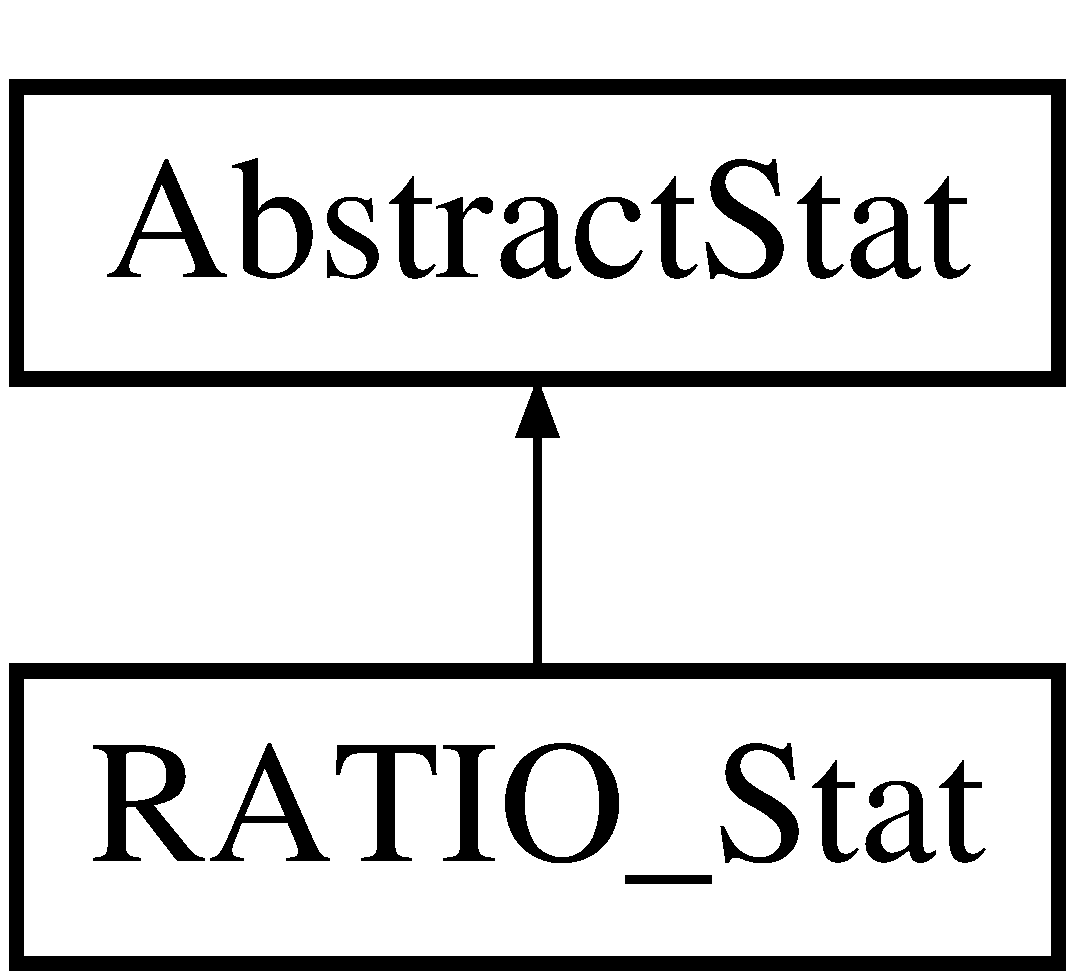
\includegraphics[height=2.000000cm]{classRATIO__Stat}
\end{center}
\end{figure}
\subsection*{Public Member Functions}
\begin{DoxyCompactItemize}
\item 
\hyperlink{classRATIO__Stat_a4f4a78937a9e1c409fd1bffd69b19869}{RATIO\_\-Stat} (const string \&str, const string \&outputfilename, long ID, long RatioID, \hyperlink{classProcessorStatistics}{ProcessorStatistics} $\ast$procStat)
\item 
virtual \hyperlink{classRATIO__Stat_a5adc98be975fc5f84f0de874a188cf68}{$\sim$RATIO\_\-Stat} ()
\item 
virtual \hyperlink{classAbstractStat}{AbstractStat} $\ast$ \hyperlink{classRATIO__Stat_af0050320d2f308a6c076992e52c9ad27}{clone} (unsigned int coreID)
\item 
void \hyperlink{classRATIO__Stat_a5b5a26cf2443e041d5c5988e9ffa6c05}{setRatioReference} (long ID)
\item 
virtual void \hyperlink{classRATIO__Stat_a0bf776a3a5dbd304185c2fce9d04934e}{writeTo} (ofstream \&stream)
\end{DoxyCompactItemize}
\subsection*{Private Attributes}
\begin{DoxyCompactItemize}
\item 
long \hyperlink{classRATIO__Stat_ad9389292fb4a07b1c5495e4e25ba0ecc}{m\_\-RatioID}
\item 
float \hyperlink{classRATIO__Stat_acf9ee3f1943b126e2d824117de380a28}{ratio}
\item 
\hyperlink{classProcessorStatistics}{ProcessorStatistics} $\ast$ \hyperlink{classRATIO__Stat_a1b31197fd3cb0740bdb32d50c4daec4c}{m\_\-ProcStat}
\end{DoxyCompactItemize}


\subsection{Detailed Description}
RATIO type stat. 

\subsection{Constructor \& Destructor Documentation}
\hypertarget{classRATIO__Stat_a4f4a78937a9e1c409fd1bffd69b19869}{
\index{RATIO\_\-Stat@{RATIO\_\-Stat}!RATIO\_\-Stat@{RATIO\_\-Stat}}
\index{RATIO\_\-Stat@{RATIO\_\-Stat}!RATIO_Stat@{RATIO\_\-Stat}}
\subsubsection[{RATIO\_\-Stat}]{\setlength{\rightskip}{0pt plus 5cm}RATIO\_\-Stat::RATIO\_\-Stat (
\begin{DoxyParamCaption}
\item[{const string \&}]{ str, }
\item[{const string \&}]{ outputfilename, }
\item[{long}]{ ID, }
\item[{long}]{ RatioID, }
\item[{{\bf ProcessorStatistics} $\ast$}]{ procStat}
\end{DoxyParamCaption}
)\hspace{0.3cm}{\ttfamily  \mbox{[}inline\mbox{]}}}}
\label{classRATIO__Stat_a4f4a78937a9e1c409fd1bffd69b19869}
Constructor. \hypertarget{classRATIO__Stat_a5adc98be975fc5f84f0de874a188cf68}{
\index{RATIO\_\-Stat@{RATIO\_\-Stat}!$\sim$RATIO\_\-Stat@{$\sim$RATIO\_\-Stat}}
\index{$\sim$RATIO\_\-Stat@{$\sim$RATIO\_\-Stat}!RATIO_Stat@{RATIO\_\-Stat}}
\subsubsection[{$\sim$RATIO\_\-Stat}]{\setlength{\rightskip}{0pt plus 5cm}virtual RATIO\_\-Stat::$\sim$RATIO\_\-Stat (
\begin{DoxyParamCaption}
{}
\end{DoxyParamCaption}
)\hspace{0.3cm}{\ttfamily  \mbox{[}inline, virtual\mbox{]}}}}
\label{classRATIO__Stat_a5adc98be975fc5f84f0de874a188cf68}
Destructor. 

\subsection{Member Function Documentation}
\hypertarget{classRATIO__Stat_af0050320d2f308a6c076992e52c9ad27}{
\index{RATIO\_\-Stat@{RATIO\_\-Stat}!clone@{clone}}
\index{clone@{clone}!RATIO_Stat@{RATIO\_\-Stat}}
\subsubsection[{clone}]{\setlength{\rightskip}{0pt plus 5cm}virtual {\bf AbstractStat}$\ast$ RATIO\_\-Stat::clone (
\begin{DoxyParamCaption}
\item[{unsigned int}]{ coreID}
\end{DoxyParamCaption}
)\hspace{0.3cm}{\ttfamily  \mbox{[}inline, virtual\mbox{]}}}}
\label{classRATIO__Stat_af0050320d2f308a6c076992e52c9ad27}
Clone a stat. 

Implements \hyperlink{classAbstractStat_aed9a458491d92fb2cc3c458990d9fab1}{AbstractStat}.

\hypertarget{classRATIO__Stat_a5b5a26cf2443e041d5c5988e9ffa6c05}{
\index{RATIO\_\-Stat@{RATIO\_\-Stat}!setRatioReference@{setRatioReference}}
\index{setRatioReference@{setRatioReference}!RATIO_Stat@{RATIO\_\-Stat}}
\subsubsection[{setRatioReference}]{\setlength{\rightskip}{0pt plus 5cm}void RATIO\_\-Stat::setRatioReference (
\begin{DoxyParamCaption}
\item[{long}]{ ID}
\end{DoxyParamCaption}
)\hspace{0.3cm}{\ttfamily  \mbox{[}inline\mbox{]}}}}
\label{classRATIO__Stat_a5b5a26cf2443e041d5c5988e9ffa6c05}
Set ratio reference id. \hypertarget{classRATIO__Stat_a0bf776a3a5dbd304185c2fce9d04934e}{
\index{RATIO\_\-Stat@{RATIO\_\-Stat}!writeTo@{writeTo}}
\index{writeTo@{writeTo}!RATIO_Stat@{RATIO\_\-Stat}}
\subsubsection[{writeTo}]{\setlength{\rightskip}{0pt plus 5cm}virtual void RATIO\_\-Stat::writeTo (
\begin{DoxyParamCaption}
\item[{ofstream \&}]{ stream}
\end{DoxyParamCaption}
)\hspace{0.3cm}{\ttfamily  \mbox{[}inline, virtual\mbox{]}}}}
\label{classRATIO__Stat_a0bf776a3a5dbd304185c2fce9d04934e}
Dump out all stats to the file. 

Reimplemented from \hyperlink{classAbstractStat_aa4760247da47c70d7345de5d881f59cb}{AbstractStat}.



\subsection{Member Data Documentation}
\hypertarget{classRATIO__Stat_a1b31197fd3cb0740bdb32d50c4daec4c}{
\index{RATIO\_\-Stat@{RATIO\_\-Stat}!m\_\-ProcStat@{m\_\-ProcStat}}
\index{m\_\-ProcStat@{m\_\-ProcStat}!RATIO_Stat@{RATIO\_\-Stat}}
\subsubsection[{m\_\-ProcStat}]{\setlength{\rightskip}{0pt plus 5cm}{\bf ProcessorStatistics}$\ast$ {\bf RATIO\_\-Stat::m\_\-ProcStat}\hspace{0.3cm}{\ttfamily  \mbox{[}private\mbox{]}}}}
\label{classRATIO__Stat_a1b31197fd3cb0740bdb32d50c4daec4c}
reference to simulation-\/scoped processor stats \hypertarget{classRATIO__Stat_ad9389292fb4a07b1c5495e4e25ba0ecc}{
\index{RATIO\_\-Stat@{RATIO\_\-Stat}!m\_\-RatioID@{m\_\-RatioID}}
\index{m\_\-RatioID@{m\_\-RatioID}!RATIO_Stat@{RATIO\_\-Stat}}
\subsubsection[{m\_\-RatioID}]{\setlength{\rightskip}{0pt plus 5cm}long {\bf RATIO\_\-Stat::m\_\-RatioID}\hspace{0.3cm}{\ttfamily  \mbox{[}private\mbox{]}}}}
\label{classRATIO__Stat_ad9389292fb4a07b1c5495e4e25ba0ecc}
ratio id \hypertarget{classRATIO__Stat_acf9ee3f1943b126e2d824117de380a28}{
\index{RATIO\_\-Stat@{RATIO\_\-Stat}!ratio@{ratio}}
\index{ratio@{ratio}!RATIO_Stat@{RATIO\_\-Stat}}
\subsubsection[{ratio}]{\setlength{\rightskip}{0pt plus 5cm}float {\bf RATIO\_\-Stat::ratio}\hspace{0.3cm}{\ttfamily  \mbox{[}private\mbox{]}}}}
\label{classRATIO__Stat_acf9ee3f1943b126e2d824117de380a28}
ratio 

The documentation for this class was generated from the following file:\begin{DoxyCompactItemize}
\item 
statistics.h\end{DoxyCompactItemize}

\hypertarget{classreadonly__cache__c}{
\section{readonly\_\-cache\_\-c Class Reference}
\label{classreadonly__cache__c}\index{readonly\_\-cache\_\-c@{readonly\_\-cache\_\-c}}
}


Readonly cache (Model GPU's constant/texture cache).  




{\ttfamily \#include $<$readonly\_\-cache.h$>$}

\subsection*{Public Member Functions}
\begin{DoxyCompactItemize}
\item 
\hypertarget{classreadonly__cache__c_aeeec3807fcbdf17fd773bbf1969e3d34}{
\hyperlink{classreadonly__cache__c_aeeec3807fcbdf17fd773bbf1969e3d34}{readonly\_\-cache\_\-c} (string name, int c\_\-id, uns32 c\_\-size, uns8 c\_\-assoc, uns8 c\_\-line\_\-size, uns8 c\_\-banks, uns8 c\_\-cycles, bool by\_\-pass, Cache\_\-Type c\_\-type, int c\_\-data\_\-size, \hyperlink{classmacsim__c}{macsim\_\-c} $\ast$simBase)}
\label{classreadonly__cache__c_aeeec3807fcbdf17fd773bbf1969e3d34}

\begin{DoxyCompactList}\small\item\em constructor to create a read-\/only cache \item\end{DoxyCompactList}\item 
\hypertarget{classreadonly__cache__c_a047b835398739dad94617f3b054065bf}{
\hyperlink{classreadonly__cache__c_a047b835398739dad94617f3b054065bf}{$\sim$readonly\_\-cache\_\-c} ()}
\label{classreadonly__cache__c_a047b835398739dad94617f3b054065bf}

\begin{DoxyCompactList}\small\item\em destructor for class \hyperlink{classreadonly__cache__c}{readonly\_\-cache\_\-c} \item\end{DoxyCompactList}\item 
int \hyperlink{classreadonly__cache__c_a98b0277cadd6d69a00117308f8a6240a}{load} (\hyperlink{classuop__c}{uop\_\-c} $\ast$uop)
\begin{DoxyCompactList}\small\item\em access read-\/only cache \item\end{DoxyCompactList}\item 
bool \hyperlink{classreadonly__cache__c_a39ccea777d82b408e93204a36be6e62b}{cache\_\-fill\_\-line} (\hyperlink{structmem__req__s}{mem\_\-req\_\-s} $\ast$req)
\begin{DoxyCompactList}\small\item\em fill read-\/only cache with cache block fetched from memory \item\end{DoxyCompactList}\item 
Addr \hyperlink{classreadonly__cache__c_a97bd29bf671a12227a4e8ba873b2c75d}{base\_\-cache\_\-line} (Addr addr)
\begin{DoxyCompactList}\small\item\em get the address of the cache line containing the specified address \item\end{DoxyCompactList}\item 
uns8 \hyperlink{classreadonly__cache__c_aecef923fdc8f384600267fcbe2f69b3b}{cache\_\-line\_\-size} (void)
\begin{DoxyCompactList}\small\item\em returns the cache block size for this cache \item\end{DoxyCompactList}\end{DoxyCompactItemize}
\subsection*{Private Attributes}
\begin{DoxyCompactItemize}
\item 
int \hyperlink{classreadonly__cache__c_aa9d46b912ab4891761ec80c32b78fe10}{m\_\-core\_\-id}
\item 
uns32 \hyperlink{classreadonly__cache__c_ab63998be492167f946e18aeb53daa14c}{m\_\-cache\_\-size}
\item 
uns8 \hyperlink{classreadonly__cache__c_a8f7344dfc8e89d9db850b03a6b319fe3}{m\_\-cache\_\-assoc}
\item 
uns8 \hyperlink{classreadonly__cache__c_a1159ba39733659b1437142c5d7ed1c4e}{m\_\-cache\_\-line\_\-size}
\item 
uns8 \hyperlink{classreadonly__cache__c_a2dca3a5ba418a2c288759418f61c2eea}{m\_\-cache\_\-banks}
\item 
uns8 \hyperlink{classreadonly__cache__c_aeb1e6fce6d78c38e6380f63723dd61a0}{m\_\-cache\_\-cycles}
\item 
Cache\_\-Type \hyperlink{classreadonly__cache__c_a84e49e7c8da3be313a17d738810686b2}{m\_\-cache\_\-type}
\item 
\hyperlink{classcache__c}{cache\_\-c} $\ast$ \hyperlink{classreadonly__cache__c_a3973be1de758a507d08771f9cf07e70b}{m\_\-cache}
\item 
\hyperlink{classmacsim__c}{macsim\_\-c} $\ast$ \hyperlink{classreadonly__cache__c_a80c6f668796ad6a9184df23a3a2e6430}{m\_\-simBase}
\end{DoxyCompactItemize}


\subsection{Detailed Description}
Readonly cache (Model GPU's constant/texture cache). class for read-\/only cache. read-\/only means that the core cannot write to cache blocks in the cache, core can only perform read-\/only accesses. in case of a cache miss, the missing cache block will be fetched from memory 

\subsection{Member Function Documentation}
\hypertarget{classreadonly__cache__c_a97bd29bf671a12227a4e8ba873b2c75d}{
\index{readonly\_\-cache\_\-c@{readonly\_\-cache\_\-c}!base\_\-cache\_\-line@{base\_\-cache\_\-line}}
\index{base\_\-cache\_\-line@{base\_\-cache\_\-line}!readonly_cache_c@{readonly\_\-cache\_\-c}}
\subsubsection[{base\_\-cache\_\-line}]{\setlength{\rightskip}{0pt plus 5cm}readonly\_\-cache\_\-c::base\_\-cache\_\-line (
\begin{DoxyParamCaption}
\item[{Addr}]{ addr}
\end{DoxyParamCaption}
)}}
\label{classreadonly__cache__c_a97bd29bf671a12227a4e8ba873b2c75d}


get the address of the cache line containing the specified address 


\begin{DoxyParams}{Parameters}
\item[{\em addr}]-\/ address whose cache line address is required \end{DoxyParams}
\begin{DoxyReturn}{Returns}
Addr -\/ requested cache line address 
\end{DoxyReturn}
\hypertarget{classreadonly__cache__c_a39ccea777d82b408e93204a36be6e62b}{
\index{readonly\_\-cache\_\-c@{readonly\_\-cache\_\-c}!cache\_\-fill\_\-line@{cache\_\-fill\_\-line}}
\index{cache\_\-fill\_\-line@{cache\_\-fill\_\-line}!readonly_cache_c@{readonly\_\-cache\_\-c}}
\subsubsection[{cache\_\-fill\_\-line}]{\setlength{\rightskip}{0pt plus 5cm}readonly\_\-cache\_\-c::cache\_\-fill\_\-line (
\begin{DoxyParamCaption}
\item[{{\bf mem\_\-req\_\-s} $\ast$}]{ req}
\end{DoxyParamCaption}
)}}
\label{classreadonly__cache__c_a39ccea777d82b408e93204a36be6e62b}


fill read-\/only cache with cache block fetched from memory 


\begin{DoxyParams}{Parameters}
\item[{\em req}]-\/ pointer to memory request \end{DoxyParams}
\begin{DoxyReturn}{Returns}
int -\/ 
\end{DoxyReturn}
\hypertarget{classreadonly__cache__c_aecef923fdc8f384600267fcbe2f69b3b}{
\index{readonly\_\-cache\_\-c@{readonly\_\-cache\_\-c}!cache\_\-line\_\-size@{cache\_\-line\_\-size}}
\index{cache\_\-line\_\-size@{cache\_\-line\_\-size}!readonly_cache_c@{readonly\_\-cache\_\-c}}
\subsubsection[{cache\_\-line\_\-size}]{\setlength{\rightskip}{0pt plus 5cm}readonly\_\-cache\_\-c::cache\_\-line\_\-size (
\begin{DoxyParamCaption}
\item[{void}]{}
\end{DoxyParamCaption}
)}}
\label{classreadonly__cache__c_aecef923fdc8f384600267fcbe2f69b3b}


returns the cache block size for this cache 

\begin{DoxyReturn}{Returns}
cache block size 
\end{DoxyReturn}
\hypertarget{classreadonly__cache__c_a98b0277cadd6d69a00117308f8a6240a}{
\index{readonly\_\-cache\_\-c@{readonly\_\-cache\_\-c}!load@{load}}
\index{load@{load}!readonly_cache_c@{readonly\_\-cache\_\-c}}
\subsubsection[{load}]{\setlength{\rightskip}{0pt plus 5cm}readonly\_\-cache\_\-c::load (
\begin{DoxyParamCaption}
\item[{{\bf uop\_\-c} $\ast$}]{ uop}
\end{DoxyParamCaption}
)}}
\label{classreadonly__cache__c_a98b0277cadd6d69a00117308f8a6240a}


access read-\/only cache 


\begin{DoxyParams}{Parameters}
\item[{\em uop}]-\/ pointer to uop which requires access to the read-\/only cache \end{DoxyParams}
\begin{DoxyReturn}{Returns}
int -\/ 
\end{DoxyReturn}


\subsection{Member Data Documentation}
\hypertarget{classreadonly__cache__c_a3973be1de758a507d08771f9cf07e70b}{
\index{readonly\_\-cache\_\-c@{readonly\_\-cache\_\-c}!m\_\-cache@{m\_\-cache}}
\index{m\_\-cache@{m\_\-cache}!readonly_cache_c@{readonly\_\-cache\_\-c}}
\subsubsection[{m\_\-cache}]{\setlength{\rightskip}{0pt plus 5cm}{\bf cache\_\-c}$\ast$ {\bf readonly\_\-cache\_\-c::m\_\-cache}\hspace{0.3cm}{\ttfamily  \mbox{[}private\mbox{]}}}}
\label{classreadonly__cache__c_a3973be1de758a507d08771f9cf07e70b}
cache data structure \hypertarget{classreadonly__cache__c_a8f7344dfc8e89d9db850b03a6b319fe3}{
\index{readonly\_\-cache\_\-c@{readonly\_\-cache\_\-c}!m\_\-cache\_\-assoc@{m\_\-cache\_\-assoc}}
\index{m\_\-cache\_\-assoc@{m\_\-cache\_\-assoc}!readonly_cache_c@{readonly\_\-cache\_\-c}}
\subsubsection[{m\_\-cache\_\-assoc}]{\setlength{\rightskip}{0pt plus 5cm}uns8 {\bf readonly\_\-cache\_\-c::m\_\-cache\_\-assoc}\hspace{0.3cm}{\ttfamily  \mbox{[}private\mbox{]}}}}
\label{classreadonly__cache__c_a8f7344dfc8e89d9db850b03a6b319fe3}
associativity \hypertarget{classreadonly__cache__c_a2dca3a5ba418a2c288759418f61c2eea}{
\index{readonly\_\-cache\_\-c@{readonly\_\-cache\_\-c}!m\_\-cache\_\-banks@{m\_\-cache\_\-banks}}
\index{m\_\-cache\_\-banks@{m\_\-cache\_\-banks}!readonly_cache_c@{readonly\_\-cache\_\-c}}
\subsubsection[{m\_\-cache\_\-banks}]{\setlength{\rightskip}{0pt plus 5cm}uns8 {\bf readonly\_\-cache\_\-c::m\_\-cache\_\-banks}\hspace{0.3cm}{\ttfamily  \mbox{[}private\mbox{]}}}}
\label{classreadonly__cache__c_a2dca3a5ba418a2c288759418f61c2eea}
number of cache banks \hypertarget{classreadonly__cache__c_aeb1e6fce6d78c38e6380f63723dd61a0}{
\index{readonly\_\-cache\_\-c@{readonly\_\-cache\_\-c}!m\_\-cache\_\-cycles@{m\_\-cache\_\-cycles}}
\index{m\_\-cache\_\-cycles@{m\_\-cache\_\-cycles}!readonly_cache_c@{readonly\_\-cache\_\-c}}
\subsubsection[{m\_\-cache\_\-cycles}]{\setlength{\rightskip}{0pt plus 5cm}uns8 {\bf readonly\_\-cache\_\-c::m\_\-cache\_\-cycles}\hspace{0.3cm}{\ttfamily  \mbox{[}private\mbox{]}}}}
\label{classreadonly__cache__c_aeb1e6fce6d78c38e6380f63723dd61a0}
cache latency \hypertarget{classreadonly__cache__c_a1159ba39733659b1437142c5d7ed1c4e}{
\index{readonly\_\-cache\_\-c@{readonly\_\-cache\_\-c}!m\_\-cache\_\-line\_\-size@{m\_\-cache\_\-line\_\-size}}
\index{m\_\-cache\_\-line\_\-size@{m\_\-cache\_\-line\_\-size}!readonly_cache_c@{readonly\_\-cache\_\-c}}
\subsubsection[{m\_\-cache\_\-line\_\-size}]{\setlength{\rightskip}{0pt plus 5cm}uns8 {\bf readonly\_\-cache\_\-c::m\_\-cache\_\-line\_\-size}\hspace{0.3cm}{\ttfamily  \mbox{[}private\mbox{]}}}}
\label{classreadonly__cache__c_a1159ba39733659b1437142c5d7ed1c4e}
cache line size \hypertarget{classreadonly__cache__c_ab63998be492167f946e18aeb53daa14c}{
\index{readonly\_\-cache\_\-c@{readonly\_\-cache\_\-c}!m\_\-cache\_\-size@{m\_\-cache\_\-size}}
\index{m\_\-cache\_\-size@{m\_\-cache\_\-size}!readonly_cache_c@{readonly\_\-cache\_\-c}}
\subsubsection[{m\_\-cache\_\-size}]{\setlength{\rightskip}{0pt plus 5cm}uns32 {\bf readonly\_\-cache\_\-c::m\_\-cache\_\-size}\hspace{0.3cm}{\ttfamily  \mbox{[}private\mbox{]}}}}
\label{classreadonly__cache__c_ab63998be492167f946e18aeb53daa14c}
cache size \hypertarget{classreadonly__cache__c_a84e49e7c8da3be313a17d738810686b2}{
\index{readonly\_\-cache\_\-c@{readonly\_\-cache\_\-c}!m\_\-cache\_\-type@{m\_\-cache\_\-type}}
\index{m\_\-cache\_\-type@{m\_\-cache\_\-type}!readonly_cache_c@{readonly\_\-cache\_\-c}}
\subsubsection[{m\_\-cache\_\-type}]{\setlength{\rightskip}{0pt plus 5cm}Cache\_\-Type {\bf readonly\_\-cache\_\-c::m\_\-cache\_\-type}\hspace{0.3cm}{\ttfamily  \mbox{[}private\mbox{]}}}}
\label{classreadonly__cache__c_a84e49e7c8da3be313a17d738810686b2}
cache type \hypertarget{classreadonly__cache__c_aa9d46b912ab4891761ec80c32b78fe10}{
\index{readonly\_\-cache\_\-c@{readonly\_\-cache\_\-c}!m\_\-core\_\-id@{m\_\-core\_\-id}}
\index{m\_\-core\_\-id@{m\_\-core\_\-id}!readonly_cache_c@{readonly\_\-cache\_\-c}}
\subsubsection[{m\_\-core\_\-id}]{\setlength{\rightskip}{0pt plus 5cm}int {\bf readonly\_\-cache\_\-c::m\_\-core\_\-id}\hspace{0.3cm}{\ttfamily  \mbox{[}private\mbox{]}}}}
\label{classreadonly__cache__c_aa9d46b912ab4891761ec80c32b78fe10}
core id \hypertarget{classreadonly__cache__c_a80c6f668796ad6a9184df23a3a2e6430}{
\index{readonly\_\-cache\_\-c@{readonly\_\-cache\_\-c}!m\_\-simBase@{m\_\-simBase}}
\index{m\_\-simBase@{m\_\-simBase}!readonly_cache_c@{readonly\_\-cache\_\-c}}
\subsubsection[{m\_\-simBase}]{\setlength{\rightskip}{0pt plus 5cm}{\bf macsim\_\-c}$\ast$ {\bf readonly\_\-cache\_\-c::m\_\-simBase}\hspace{0.3cm}{\ttfamily  \mbox{[}private\mbox{]}}}}
\label{classreadonly__cache__c_a80c6f668796ad6a9184df23a3a2e6430}
\hyperlink{classmacsim__c}{macsim\_\-c} base class for simulation globals 

The documentation for this class was generated from the following files:\begin{DoxyCompactItemize}
\item 
readonly\_\-cache.h\item 
readonly\_\-cache.cc\end{DoxyCompactItemize}

\hypertarget{structreconv__data__s}{
\section{reconv\_\-data\_\-s Struct Reference}
\label{structreconv__data__s}\index{reconv\_\-data\_\-s@{reconv\_\-data\_\-s}}
}


reconvergence data  




{\ttfamily \#include $<$frontend.h$>$}

\subsection*{Public Attributes}
\begin{DoxyCompactItemize}
\item 
int32\_\-t \hyperlink{structreconv__data__s_ac79260e63c70c3ed072a91b31d0744d1}{m\_\-work\_\-counter}
\item 
int32\_\-t \hyperlink{structreconv__data__s_a1b2d372adb1e9920c6a37fd3e1b72a77}{m\_\-reconverge\_\-depth}
\item 
int32\_\-t \hyperlink{structreconv__data__s_a14a215431914767f23ecd5529a02ccac}{m\_\-top\_\-level\_\-reconv\_\-seen}
\end{DoxyCompactItemize}


\subsection{Detailed Description}
reconvergence data 

\subsection{Member Data Documentation}
\hypertarget{structreconv__data__s_a1b2d372adb1e9920c6a37fd3e1b72a77}{
\index{reconv\_\-data\_\-s@{reconv\_\-data\_\-s}!m\_\-reconverge\_\-depth@{m\_\-reconverge\_\-depth}}
\index{m\_\-reconverge\_\-depth@{m\_\-reconverge\_\-depth}!reconv_data_s@{reconv\_\-data\_\-s}}
\subsubsection[{m\_\-reconverge\_\-depth}]{\setlength{\rightskip}{0pt plus 5cm}int32\_\-t {\bf reconv\_\-data\_\-s::m\_\-reconverge\_\-depth}}}
\label{structreconv__data__s_a1b2d372adb1e9920c6a37fd3e1b72a77}
reconvergence depth \hypertarget{structreconv__data__s_a14a215431914767f23ecd5529a02ccac}{
\index{reconv\_\-data\_\-s@{reconv\_\-data\_\-s}!m\_\-top\_\-level\_\-reconv\_\-seen@{m\_\-top\_\-level\_\-reconv\_\-seen}}
\index{m\_\-top\_\-level\_\-reconv\_\-seen@{m\_\-top\_\-level\_\-reconv\_\-seen}!reconv_data_s@{reconv\_\-data\_\-s}}
\subsubsection[{m\_\-top\_\-level\_\-reconv\_\-seen}]{\setlength{\rightskip}{0pt plus 5cm}int32\_\-t {\bf reconv\_\-data\_\-s::m\_\-top\_\-level\_\-reconv\_\-seen}}}
\label{structreconv__data__s_a14a215431914767f23ecd5529a02ccac}
top level reconvergence seen \hypertarget{structreconv__data__s_ac79260e63c70c3ed072a91b31d0744d1}{
\index{reconv\_\-data\_\-s@{reconv\_\-data\_\-s}!m\_\-work\_\-counter@{m\_\-work\_\-counter}}
\index{m\_\-work\_\-counter@{m\_\-work\_\-counter}!reconv_data_s@{reconv\_\-data\_\-s}}
\subsubsection[{m\_\-work\_\-counter}]{\setlength{\rightskip}{0pt plus 5cm}int32\_\-t {\bf reconv\_\-data\_\-s::m\_\-work\_\-counter}}}
\label{structreconv__data__s_ac79260e63c70c3ed072a91b31d0744d1}
work counter 

The documentation for this struct was generated from the following file:\begin{DoxyCompactItemize}
\item 
frontend.h\end{DoxyCompactItemize}

\hypertarget{classrecovery__info__c}{
\section{recovery\_\-info\_\-c Class Reference}
\label{classrecovery__info__c}\index{recovery\_\-info\_\-c@{recovery\_\-info\_\-c}}
}


branch misprediction recovery information  




{\ttfamily \#include $<$uop.h$>$}

\subsection*{Public Member Functions}
\begin{DoxyCompactItemize}
\item 
\hyperlink{classrecovery__info__c_a47f03dbfec8ad3a53274a0d63b8e08c3}{recovery\_\-info\_\-c} ()
\item 
\hyperlink{classrecovery__info__c_a76ba8f1a24189ddd876c5eb08cf2fc4a}{$\sim$recovery\_\-info\_\-c} ()
\end{DoxyCompactItemize}
\subsection*{Public Attributes}
\begin{DoxyCompactItemize}
\item 
uns32 \hyperlink{classrecovery__info__c_aa4e7499fc8b15e669f054591f65ac457}{m\_\-global\_\-hist}
\item 
uns64 \hyperlink{classrecovery__info__c_ae900e8c2b0de1acdfa6ddd05419d2ceb}{m\_\-global\_\-hist\_\-64}
\item 
int \hyperlink{classrecovery__info__c_a2d39830ee723d6c7d34f3c7ced497bdf}{m\_\-thread\_\-id}
\end{DoxyCompactItemize}


\subsection{Detailed Description}
branch misprediction recovery information 

\subsection{Constructor \& Destructor Documentation}
\hypertarget{classrecovery__info__c_a47f03dbfec8ad3a53274a0d63b8e08c3}{
\index{recovery\_\-info\_\-c@{recovery\_\-info\_\-c}!recovery\_\-info\_\-c@{recovery\_\-info\_\-c}}
\index{recovery\_\-info\_\-c@{recovery\_\-info\_\-c}!recovery_info_c@{recovery\_\-info\_\-c}}
\subsubsection[{recovery\_\-info\_\-c}]{\setlength{\rightskip}{0pt plus 5cm}recovery\_\-info\_\-c::recovery\_\-info\_\-c (
\begin{DoxyParamCaption}
{}
\end{DoxyParamCaption}
)\hspace{0.3cm}{\ttfamily  \mbox{[}inline\mbox{]}}}}
\label{classrecovery__info__c_a47f03dbfec8ad3a53274a0d63b8e08c3}
Constructor \hypertarget{classrecovery__info__c_a76ba8f1a24189ddd876c5eb08cf2fc4a}{
\index{recovery\_\-info\_\-c@{recovery\_\-info\_\-c}!$\sim$recovery\_\-info\_\-c@{$\sim$recovery\_\-info\_\-c}}
\index{$\sim$recovery\_\-info\_\-c@{$\sim$recovery\_\-info\_\-c}!recovery_info_c@{recovery\_\-info\_\-c}}
\subsubsection[{$\sim$recovery\_\-info\_\-c}]{\setlength{\rightskip}{0pt plus 5cm}recovery\_\-info\_\-c::$\sim$recovery\_\-info\_\-c (
\begin{DoxyParamCaption}
{}
\end{DoxyParamCaption}
)\hspace{0.3cm}{\ttfamily  \mbox{[}inline\mbox{]}}}}
\label{classrecovery__info__c_a76ba8f1a24189ddd876c5eb08cf2fc4a}
Destructor 

\subsection{Member Data Documentation}
\hypertarget{classrecovery__info__c_aa4e7499fc8b15e669f054591f65ac457}{
\index{recovery\_\-info\_\-c@{recovery\_\-info\_\-c}!m\_\-global\_\-hist@{m\_\-global\_\-hist}}
\index{m\_\-global\_\-hist@{m\_\-global\_\-hist}!recovery_info_c@{recovery\_\-info\_\-c}}
\subsubsection[{m\_\-global\_\-hist}]{\setlength{\rightskip}{0pt plus 5cm}uns32 {\bf recovery\_\-info\_\-c::m\_\-global\_\-hist}}}
\label{classrecovery__info__c_aa4e7499fc8b15e669f054591f65ac457}
global branch history 32-\/bit \hypertarget{classrecovery__info__c_ae900e8c2b0de1acdfa6ddd05419d2ceb}{
\index{recovery\_\-info\_\-c@{recovery\_\-info\_\-c}!m\_\-global\_\-hist\_\-64@{m\_\-global\_\-hist\_\-64}}
\index{m\_\-global\_\-hist\_\-64@{m\_\-global\_\-hist\_\-64}!recovery_info_c@{recovery\_\-info\_\-c}}
\subsubsection[{m\_\-global\_\-hist\_\-64}]{\setlength{\rightskip}{0pt plus 5cm}uns64 {\bf recovery\_\-info\_\-c::m\_\-global\_\-hist\_\-64}}}
\label{classrecovery__info__c_ae900e8c2b0de1acdfa6ddd05419d2ceb}
global branch history 64-\/bit \hypertarget{classrecovery__info__c_a2d39830ee723d6c7d34f3c7ced497bdf}{
\index{recovery\_\-info\_\-c@{recovery\_\-info\_\-c}!m\_\-thread\_\-id@{m\_\-thread\_\-id}}
\index{m\_\-thread\_\-id@{m\_\-thread\_\-id}!recovery_info_c@{recovery\_\-info\_\-c}}
\subsubsection[{m\_\-thread\_\-id}]{\setlength{\rightskip}{0pt plus 5cm}int {\bf recovery\_\-info\_\-c::m\_\-thread\_\-id}}}
\label{classrecovery__info__c_a2d39830ee723d6c7d34f3c7ced497bdf}
thread id 

The documentation for this class was generated from the following file:\begin{DoxyCompactItemize}
\item 
uop.h\end{DoxyCompactItemize}

\hypertarget{structreg__info__s}{
\section{reg\_\-info\_\-s Struct Reference}
\label{structreg__info__s}\index{reg\_\-info\_\-s@{reg\_\-info\_\-s}}
}


Register information data structure.  




{\ttfamily \#include $<$inst\_\-info.h$>$}

\subsection*{Public Member Functions}
\begin{DoxyCompactItemize}
\item 
\hyperlink{structreg__info__s_a868de813f36a320d6a67dfba5548b90e}{reg\_\-info\_\-s} ()
\end{DoxyCompactItemize}
\subsection*{Public Attributes}
\begin{DoxyCompactItemize}
\item 
\hypertarget{structreg__info__s_aed3b44e06ae0390ed062366b04b75c81}{
uns16 \hyperlink{structreg__info__s_aed3b44e06ae0390ed062366b04b75c81}{m\_\-reg}}
\label{structreg__info__s_aed3b44e06ae0390ed062366b04b75c81}

\begin{DoxyCompactList}\small\item\em register number within the register set \item\end{DoxyCompactList}\item 
\hypertarget{structreg__info__s_a86340490bcb855cb8da9c691a382d478}{
Reg\_\-Type \hyperlink{structreg__info__s_a86340490bcb855cb8da9c691a382d478}{m\_\-type}}
\label{structreg__info__s_a86340490bcb855cb8da9c691a382d478}

\begin{DoxyCompactList}\small\item\em integer, floating point, extra \item\end{DoxyCompactList}\item 
\hypertarget{structreg__info__s_a8b1cdcb766e8417c38d8d2e125d63eb1}{
uns16 \hyperlink{structreg__info__s_a8b1cdcb766e8417c38d8d2e125d63eb1}{m\_\-id}}
\label{structreg__info__s_a8b1cdcb766e8417c38d8d2e125d63eb1}

\begin{DoxyCompactList}\small\item\em flattened register number (unique across sets) \item\end{DoxyCompactList}\end{DoxyCompactItemize}


\subsection{Detailed Description}
Register information data structure. 

\subsection{Constructor \& Destructor Documentation}
\hypertarget{structreg__info__s_a868de813f36a320d6a67dfba5548b90e}{
\index{reg\_\-info\_\-s@{reg\_\-info\_\-s}!reg\_\-info\_\-s@{reg\_\-info\_\-s}}
\index{reg\_\-info\_\-s@{reg\_\-info\_\-s}!reg_info_s@{reg\_\-info\_\-s}}
\subsubsection[{reg\_\-info\_\-s}]{\setlength{\rightskip}{0pt plus 5cm}reg\_\-info\_\-s::reg\_\-info\_\-s (
\begin{DoxyParamCaption}
{}
\end{DoxyParamCaption}
)}}
\label{structreg__info__s_a868de813f36a320d6a67dfba5548b90e}
Constructor 

The documentation for this struct was generated from the following files:\begin{DoxyCompactItemize}
\item 
inst\_\-info.h\item 
trace\_\-read.cc\end{DoxyCompactItemize}

\hypertarget{classretire__c}{
\section{retire\_\-c Class Reference}
\label{classretire__c}\index{retire\_\-c@{retire\_\-c}}
}


retirement stage  




{\ttfamily \#include $<$retire.h$>$}

\subsection*{Public Member Functions}
\begin{DoxyCompactItemize}
\item 
\hyperlink{classretire__c_a5310845cf7bee50f1bbc9c2b1e731e80}{retire\_\-c} (RETIRE\_\-INTERFACE\_\-PARAMS(), \hyperlink{classmacsim__c}{macsim\_\-c} $\ast$simBase)
\item 
\hyperlink{classretire__c_a9d262d8ca4b2e9de0729d73c2c293ee7}{$\sim$retire\_\-c} ()
\item 
void \hyperlink{classretire__c_a438f9012b09989659d8ef4327f2bb77a}{run\_\-a\_\-cycle} ()
\item 
void \hyperlink{classretire__c_a818ade739285989194fda54e649cdaa3}{start} ()
\item 
void \hyperlink{classretire__c_a9e773dd9d20ce1b75f0fd169cc6ea281}{stop} ()
\item 
bool \hyperlink{classretire__c_a654a996cb34a4e5c0d37067a6790acc9}{is\_\-running} ()
\item 
Counter \hyperlink{classretire__c_a0fefc3d4fb52bd905f71e658706775a5}{get\_\-instrs\_\-retired} (int thread\_\-id)
\item 
Counter \hyperlink{classretire__c_a2e089e4af473a1d17cb7648d3e9baa10}{get\_\-uops\_\-retired} (int thread\_\-id)
\item 
Counter \hyperlink{classretire__c_ac8b2d59e8cd9a0810ba4c993254fce89}{get\_\-total\_\-insts\_\-retired} ()
\item 
void \hyperlink{classretire__c_a7625722bdf7f036d8e2fcb374801ddd2}{allocate\_\-retire\_\-data} (int)
\item 
void \hyperlink{classretire__c_afd9831ac670b912e9702abd2bb24d3c3}{deallocate\_\-retire\_\-data} (int)
\item 
\hypertarget{classretire__c_acffa17bdf1d58a503a9ecda79caa4acc}{
int {\bfseries get\_\-periodic\_\-inst\_\-count} (void)}
\label{classretire__c_acffa17bdf1d58a503a9ecda79caa4acc}

\end{DoxyCompactItemize}
\subsection*{Private Member Functions}
\begin{DoxyCompactItemize}
\item 
\hyperlink{classretire__c_a07e9117cffbab18595be92616ec1852b}{retire\_\-c} (const \hyperlink{classretire__c}{retire\_\-c} \&rhs)
\item 
\hyperlink{classretire__c}{retire\_\-c} \& \hyperlink{classretire__c_a4d74507c105952708d0b88ae198c456b}{operator=} (const \hyperlink{classretire__c}{retire\_\-c} \&rhs)
\item 
void \hyperlink{classretire__c_a20e4b31657c49da538d1360c060f7776}{update\_\-stats} (\hyperlink{structprocess__s}{process\_\-s} $\ast$)
\item 
void \hyperlink{classretire__c_aad999812f5d299edc5426613393b552e}{repeat\_\-traces} (\hyperlink{structprocess__s}{process\_\-s} $\ast$)
\item 
\hypertarget{classretire__c_af40a5cf3a5b9be53a30b37997db162bf}{
{\bfseries RETIRE\_\-INTERFACE\_\-DECL} ()}
\label{classretire__c_af40a5cf3a5b9be53a30b37997db162bf}

\end{DoxyCompactItemize}
\subsection*{Private Attributes}
\begin{DoxyCompactItemize}
\item 
bool \hyperlink{classretire__c_a440ae82fa7ace4028c64aae7abc24337}{m\_\-retire\_\-running}
\item 
Counter \hyperlink{classretire__c_a59114d1649ab7872ce25636b173353aa}{m\_\-total\_\-insts\_\-retired}
\item 
Counter \hyperlink{classretire__c_af58d8582170f634d4f021b76fd958b01}{m\_\-cur\_\-core\_\-cycle}
\item 
uns16 \hyperlink{classretire__c_ae0cb9e43818642ff68a1565004cd3080}{m\_\-knob\_\-width}
\item 
bool \hyperlink{classretire__c_a08f7427294d9f9d709beb52d33e98f41}{m\_\-knob\_\-ptx\_\-sim}
\item 
unordered\_\-map$<$ int, Counter $>$ \hyperlink{classretire__c_a84318556bf044a1c3bdbd08f61fe2d3a}{m\_\-insts\_\-retired}
\item 
unordered\_\-map$<$ int, Counter $>$ \hyperlink{classretire__c_a5e284ce1f986ab38f7d337e2dc7d3977}{m\_\-uops\_\-retired}
\item 
\hypertarget{classretire__c_a7ce9fe24f3b01a20eed2f7195cdc6f9c}{
int {\bfseries m\_\-period\_\-inst\_\-count}}
\label{classretire__c_a7ce9fe24f3b01a20eed2f7195cdc6f9c}

\item 
\hyperlink{classmacsim__c}{macsim\_\-c} $\ast$ \hyperlink{classretire__c_a373e6acbae9c640abe0cfeaf54c0be53}{m\_\-simBase}
\end{DoxyCompactItemize}


\subsection{Detailed Description}
retirement stage Retire (Commit) stage in the pipeline 

\subsection{Constructor \& Destructor Documentation}
\hypertarget{classretire__c_a5310845cf7bee50f1bbc9c2b1e731e80}{
\index{retire\_\-c@{retire\_\-c}!retire\_\-c@{retire\_\-c}}
\index{retire\_\-c@{retire\_\-c}!retire_c@{retire\_\-c}}
\subsubsection[{retire\_\-c}]{\setlength{\rightskip}{0pt plus 5cm}retire\_\-c::retire\_\-c (
\begin{DoxyParamCaption}
\item[{RETIRE\_\-INTERFACE\_\-PARAMS()}]{, }
\item[{{\bf macsim\_\-c} $\ast$}]{ simBase}
\end{DoxyParamCaption}
)}}
\label{classretire__c_a5310845cf7bee50f1bbc9c2b1e731e80}
Constructor \hypertarget{classretire__c_a9d262d8ca4b2e9de0729d73c2c293ee7}{
\index{retire\_\-c@{retire\_\-c}!$\sim$retire\_\-c@{$\sim$retire\_\-c}}
\index{$\sim$retire\_\-c@{$\sim$retire\_\-c}!retire_c@{retire\_\-c}}
\subsubsection[{$\sim$retire\_\-c}]{\setlength{\rightskip}{0pt plus 5cm}retire\_\-c::$\sim$retire\_\-c (
\begin{DoxyParamCaption}
{}
\end{DoxyParamCaption}
)}}
\label{classretire__c_a9d262d8ca4b2e9de0729d73c2c293ee7}
Destructor \hypertarget{classretire__c_a07e9117cffbab18595be92616ec1852b}{
\index{retire\_\-c@{retire\_\-c}!retire\_\-c@{retire\_\-c}}
\index{retire\_\-c@{retire\_\-c}!retire_c@{retire\_\-c}}
\subsubsection[{retire\_\-c}]{\setlength{\rightskip}{0pt plus 5cm}retire\_\-c::retire\_\-c (
\begin{DoxyParamCaption}
\item[{const {\bf retire\_\-c} \&}]{ rhs}
\end{DoxyParamCaption}
)\hspace{0.3cm}{\ttfamily  \mbox{[}private\mbox{]}}}}
\label{classretire__c_a07e9117cffbab18595be92616ec1852b}
Private constructor. Do not implement 

\subsection{Member Function Documentation}
\hypertarget{classretire__c_a7625722bdf7f036d8e2fcb374801ddd2}{
\index{retire\_\-c@{retire\_\-c}!allocate\_\-retire\_\-data@{allocate\_\-retire\_\-data}}
\index{allocate\_\-retire\_\-data@{allocate\_\-retire\_\-data}!retire_c@{retire\_\-c}}
\subsubsection[{allocate\_\-retire\_\-data}]{\setlength{\rightskip}{0pt plus 5cm}void retire\_\-c::allocate\_\-retire\_\-data (
\begin{DoxyParamCaption}
\item[{int}]{ tid}
\end{DoxyParamCaption}
)}}
\label{classretire__c_a7625722bdf7f036d8e2fcb374801ddd2}
When a new thread has been scheduled, reset data \hypertarget{classretire__c_afd9831ac670b912e9702abd2bb24d3c3}{
\index{retire\_\-c@{retire\_\-c}!deallocate\_\-retire\_\-data@{deallocate\_\-retire\_\-data}}
\index{deallocate\_\-retire\_\-data@{deallocate\_\-retire\_\-data}!retire_c@{retire\_\-c}}
\subsubsection[{deallocate\_\-retire\_\-data}]{\setlength{\rightskip}{0pt plus 5cm}void retire\_\-c::deallocate\_\-retire\_\-data (
\begin{DoxyParamCaption}
\item[{int}]{}
\end{DoxyParamCaption}
)}}
\label{classretire__c_afd9831ac670b912e9702abd2bb24d3c3}
Deallocate per thread data \hypertarget{classretire__c_a0fefc3d4fb52bd905f71e658706775a5}{
\index{retire\_\-c@{retire\_\-c}!get\_\-instrs\_\-retired@{get\_\-instrs\_\-retired}}
\index{get\_\-instrs\_\-retired@{get\_\-instrs\_\-retired}!retire_c@{retire\_\-c}}
\subsubsection[{get\_\-instrs\_\-retired}]{\setlength{\rightskip}{0pt plus 5cm}Counter retire\_\-c::get\_\-instrs\_\-retired (
\begin{DoxyParamCaption}
\item[{int}]{ thread\_\-id}
\end{DoxyParamCaption}
)\hspace{0.3cm}{\ttfamily  \mbox{[}inline\mbox{]}}}}
\label{classretire__c_a0fefc3d4fb52bd905f71e658706775a5}
Get number of retired instruction with thread\_\-id \hypertarget{classretire__c_ac8b2d59e8cd9a0810ba4c993254fce89}{
\index{retire\_\-c@{retire\_\-c}!get\_\-total\_\-insts\_\-retired@{get\_\-total\_\-insts\_\-retired}}
\index{get\_\-total\_\-insts\_\-retired@{get\_\-total\_\-insts\_\-retired}!retire_c@{retire\_\-c}}
\subsubsection[{get\_\-total\_\-insts\_\-retired}]{\setlength{\rightskip}{0pt plus 5cm}Counter retire\_\-c::get\_\-total\_\-insts\_\-retired (
\begin{DoxyParamCaption}
{}
\end{DoxyParamCaption}
)}}
\label{classretire__c_ac8b2d59e8cd9a0810ba4c993254fce89}
Get number of total retired instructions \hypertarget{classretire__c_a2e089e4af473a1d17cb7648d3e9baa10}{
\index{retire\_\-c@{retire\_\-c}!get\_\-uops\_\-retired@{get\_\-uops\_\-retired}}
\index{get\_\-uops\_\-retired@{get\_\-uops\_\-retired}!retire_c@{retire\_\-c}}
\subsubsection[{get\_\-uops\_\-retired}]{\setlength{\rightskip}{0pt plus 5cm}Counter retire\_\-c::get\_\-uops\_\-retired (
\begin{DoxyParamCaption}
\item[{int}]{ thread\_\-id}
\end{DoxyParamCaption}
)}}
\label{classretire__c_a2e089e4af473a1d17cb7648d3e9baa10}
Get number of retired uops with thread\_\-id \hypertarget{classretire__c_a654a996cb34a4e5c0d37067a6790acc9}{
\index{retire\_\-c@{retire\_\-c}!is\_\-running@{is\_\-running}}
\index{is\_\-running@{is\_\-running}!retire_c@{retire\_\-c}}
\subsubsection[{is\_\-running}]{\setlength{\rightskip}{0pt plus 5cm}bool retire\_\-c::is\_\-running (
\begin{DoxyParamCaption}
{}
\end{DoxyParamCaption}
)}}
\label{classretire__c_a654a996cb34a4e5c0d37067a6790acc9}
Check retirement stage is running \hypertarget{classretire__c_a4d74507c105952708d0b88ae198c456b}{
\index{retire\_\-c@{retire\_\-c}!operator=@{operator=}}
\index{operator=@{operator=}!retire_c@{retire\_\-c}}
\subsubsection[{operator=}]{\setlength{\rightskip}{0pt plus 5cm}{\bf retire\_\-c}\& retire\_\-c::operator= (
\begin{DoxyParamCaption}
\item[{const {\bf retire\_\-c} \&}]{ rhs}
\end{DoxyParamCaption}
)\hspace{0.3cm}{\ttfamily  \mbox{[}private\mbox{]}}}}
\label{classretire__c_a4d74507c105952708d0b88ae198c456b}
Overridden operator = \hypertarget{classretire__c_aad999812f5d299edc5426613393b552e}{
\index{retire\_\-c@{retire\_\-c}!repeat\_\-traces@{repeat\_\-traces}}
\index{repeat\_\-traces@{repeat\_\-traces}!retire_c@{retire\_\-c}}
\subsubsection[{repeat\_\-traces}]{\setlength{\rightskip}{0pt plus 5cm}void retire\_\-c::repeat\_\-traces (
\begin{DoxyParamCaption}
\item[{{\bf process\_\-s} $\ast$}]{ process}
\end{DoxyParamCaption}
)\hspace{0.3cm}{\ttfamily  \mbox{[}private\mbox{]}}}}
\label{classretire__c_aad999812f5d299edc5426613393b552e}
Repeat (terminated) application \hypertarget{classretire__c_a438f9012b09989659d8ef4327f2bb77a}{
\index{retire\_\-c@{retire\_\-c}!run\_\-a\_\-cycle@{run\_\-a\_\-cycle}}
\index{run\_\-a\_\-cycle@{run\_\-a\_\-cycle}!retire_c@{retire\_\-c}}
\subsubsection[{run\_\-a\_\-cycle}]{\setlength{\rightskip}{0pt plus 5cm}void retire\_\-c::run\_\-a\_\-cycle (
\begin{DoxyParamCaption}
\item[{void}]{}
\end{DoxyParamCaption}
)}}
\label{classretire__c_a438f9012b09989659d8ef4327f2bb77a}
Tick a cycle \hypertarget{classretire__c_a818ade739285989194fda54e649cdaa3}{
\index{retire\_\-c@{retire\_\-c}!start@{start}}
\index{start@{start}!retire_c@{retire\_\-c}}
\subsubsection[{start}]{\setlength{\rightskip}{0pt plus 5cm}void retire\_\-c::start (
\begin{DoxyParamCaption}
\item[{void}]{}
\end{DoxyParamCaption}
)}}
\label{classretire__c_a818ade739285989194fda54e649cdaa3}
Enable retirement stage \hypertarget{classretire__c_a9e773dd9d20ce1b75f0fd169cc6ea281}{
\index{retire\_\-c@{retire\_\-c}!stop@{stop}}
\index{stop@{stop}!retire_c@{retire\_\-c}}
\subsubsection[{stop}]{\setlength{\rightskip}{0pt plus 5cm}void retire\_\-c::stop (
\begin{DoxyParamCaption}
\item[{void}]{}
\end{DoxyParamCaption}
)}}
\label{classretire__c_a9e773dd9d20ce1b75f0fd169cc6ea281}
Disable retirement stage \hypertarget{classretire__c_a20e4b31657c49da538d1360c060f7776}{
\index{retire\_\-c@{retire\_\-c}!update\_\-stats@{update\_\-stats}}
\index{update\_\-stats@{update\_\-stats}!retire_c@{retire\_\-c}}
\subsubsection[{update\_\-stats}]{\setlength{\rightskip}{0pt plus 5cm}void retire\_\-c::update\_\-stats (
\begin{DoxyParamCaption}
\item[{{\bf process\_\-s} $\ast$}]{ process}
\end{DoxyParamCaption}
)\hspace{0.3cm}{\ttfamily  \mbox{[}private\mbox{]}}}}
\label{classretire__c_a20e4b31657c49da538d1360c060f7776}
Update stats when an application is done 

\subsection{Member Data Documentation}
\hypertarget{classretire__c_af58d8582170f634d4f021b76fd958b01}{
\index{retire\_\-c@{retire\_\-c}!m\_\-cur\_\-core\_\-cycle@{m\_\-cur\_\-core\_\-cycle}}
\index{m\_\-cur\_\-core\_\-cycle@{m\_\-cur\_\-core\_\-cycle}!retire_c@{retire\_\-c}}
\subsubsection[{m\_\-cur\_\-core\_\-cycle}]{\setlength{\rightskip}{0pt plus 5cm}Counter {\bf retire\_\-c::m\_\-cur\_\-core\_\-cycle}\hspace{0.3cm}{\ttfamily  \mbox{[}private\mbox{]}}}}
\label{classretire__c_af58d8582170f634d4f021b76fd958b01}
current core cycle \hypertarget{classretire__c_a84318556bf044a1c3bdbd08f61fe2d3a}{
\index{retire\_\-c@{retire\_\-c}!m\_\-insts\_\-retired@{m\_\-insts\_\-retired}}
\index{m\_\-insts\_\-retired@{m\_\-insts\_\-retired}!retire_c@{retire\_\-c}}
\subsubsection[{m\_\-insts\_\-retired}]{\setlength{\rightskip}{0pt plus 5cm}unordered\_\-map$<$int, Counter$>$ {\bf retire\_\-c::m\_\-insts\_\-retired}\hspace{0.3cm}{\ttfamily  \mbox{[}private\mbox{]}}}}
\label{classretire__c_a84318556bf044a1c3bdbd08f61fe2d3a}
number of retired inst. per thread \hypertarget{classretire__c_a08f7427294d9f9d709beb52d33e98f41}{
\index{retire\_\-c@{retire\_\-c}!m\_\-knob\_\-ptx\_\-sim@{m\_\-knob\_\-ptx\_\-sim}}
\index{m\_\-knob\_\-ptx\_\-sim@{m\_\-knob\_\-ptx\_\-sim}!retire_c@{retire\_\-c}}
\subsubsection[{m\_\-knob\_\-ptx\_\-sim}]{\setlength{\rightskip}{0pt plus 5cm}bool {\bf retire\_\-c::m\_\-knob\_\-ptx\_\-sim}\hspace{0.3cm}{\ttfamily  \mbox{[}private\mbox{]}}}}
\label{classretire__c_a08f7427294d9f9d709beb52d33e98f41}
gpu simulation \hypertarget{classretire__c_ae0cb9e43818642ff68a1565004cd3080}{
\index{retire\_\-c@{retire\_\-c}!m\_\-knob\_\-width@{m\_\-knob\_\-width}}
\index{m\_\-knob\_\-width@{m\_\-knob\_\-width}!retire_c@{retire\_\-c}}
\subsubsection[{m\_\-knob\_\-width}]{\setlength{\rightskip}{0pt plus 5cm}uns16 {\bf retire\_\-c::m\_\-knob\_\-width}\hspace{0.3cm}{\ttfamily  \mbox{[}private\mbox{]}}}}
\label{classretire__c_ae0cb9e43818642ff68a1565004cd3080}
pipeline width \hypertarget{classretire__c_a440ae82fa7ace4028c64aae7abc24337}{
\index{retire\_\-c@{retire\_\-c}!m\_\-retire\_\-running@{m\_\-retire\_\-running}}
\index{m\_\-retire\_\-running@{m\_\-retire\_\-running}!retire_c@{retire\_\-c}}
\subsubsection[{m\_\-retire\_\-running}]{\setlength{\rightskip}{0pt plus 5cm}bool {\bf retire\_\-c::m\_\-retire\_\-running}\hspace{0.3cm}{\ttfamily  \mbox{[}private\mbox{]}}}}
\label{classretire__c_a440ae82fa7ace4028c64aae7abc24337}
retire enabled \hypertarget{classretire__c_a373e6acbae9c640abe0cfeaf54c0be53}{
\index{retire\_\-c@{retire\_\-c}!m\_\-simBase@{m\_\-simBase}}
\index{m\_\-simBase@{m\_\-simBase}!retire_c@{retire\_\-c}}
\subsubsection[{m\_\-simBase}]{\setlength{\rightskip}{0pt plus 5cm}{\bf macsim\_\-c}$\ast$ {\bf retire\_\-c::m\_\-simBase}\hspace{0.3cm}{\ttfamily  \mbox{[}private\mbox{]}}}}
\label{classretire__c_a373e6acbae9c640abe0cfeaf54c0be53}
\hyperlink{classmacsim__c}{macsim\_\-c} base class for simulation globals \hypertarget{classretire__c_a59114d1649ab7872ce25636b173353aa}{
\index{retire\_\-c@{retire\_\-c}!m\_\-total\_\-insts\_\-retired@{m\_\-total\_\-insts\_\-retired}}
\index{m\_\-total\_\-insts\_\-retired@{m\_\-total\_\-insts\_\-retired}!retire_c@{retire\_\-c}}
\subsubsection[{m\_\-total\_\-insts\_\-retired}]{\setlength{\rightskip}{0pt plus 5cm}Counter {\bf retire\_\-c::m\_\-total\_\-insts\_\-retired}\hspace{0.3cm}{\ttfamily  \mbox{[}private\mbox{]}}}}
\label{classretire__c_a59114d1649ab7872ce25636b173353aa}
total retired instructions \hypertarget{classretire__c_a5e284ce1f986ab38f7d337e2dc7d3977}{
\index{retire\_\-c@{retire\_\-c}!m\_\-uops\_\-retired@{m\_\-uops\_\-retired}}
\index{m\_\-uops\_\-retired@{m\_\-uops\_\-retired}!retire_c@{retire\_\-c}}
\subsubsection[{m\_\-uops\_\-retired}]{\setlength{\rightskip}{0pt plus 5cm}unordered\_\-map$<$int, Counter$>$ {\bf retire\_\-c::m\_\-uops\_\-retired}\hspace{0.3cm}{\ttfamily  \mbox{[}private\mbox{]}}}}
\label{classretire__c_a5e284ce1f986ab38f7d337e2dc7d3977}
number of retired uop per thread 

The documentation for this class was generated from the following files:\begin{DoxyCompactItemize}
\item 
retire.h\item 
retire.cc\end{DoxyCompactItemize}

\hypertarget{classrob__c}{
\section{rob\_\-c Class Reference}
\label{classrob__c}\index{rob\_\-c@{rob\_\-c}}
}


ROB (Reorder Buffer) class.  




{\ttfamily \#include $<$rob.h$>$}

\subsection*{Public Member Functions}
\begin{DoxyCompactItemize}
\item 
\hypertarget{classrob__c_ac1fb29aba19dda5309209484c680cb21}{
{\bfseries rob\_\-c} (Unit\_\-Type type, \hyperlink{classmacsim__c}{macsim\_\-c} $\ast$simBase)}
\label{classrob__c_ac1fb29aba19dda5309209484c680cb21}

\item 
\hyperlink{classrob__c_a8234eee835493946b51d12f6203b1f45}{$\sim$rob\_\-c} ()
\begin{DoxyCompactList}\small\item\em Reorder Buffer data structure destructor. \item\end{DoxyCompactList}\item 
void \hyperlink{classrob__c_a86f6d806468ba6fd74ed1eb39dbd5d2e}{push} (\hyperlink{classuop__c}{uop\_\-c} $\ast$s)
\begin{DoxyCompactList}\small\item\em Function to push an arguement into the ROB. \item\end{DoxyCompactList}\item 
void \hyperlink{classrob__c_abc83fd479320491b7d5eab296c0ef2fa}{pop} ()
\begin{DoxyCompactList}\small\item\em Function to pop an arguement off the ROB. \item\end{DoxyCompactList}\item 
void \hyperlink{classrob__c_a0a92a8da241c352e7379815f12d06f88}{reinit} ()
\begin{DoxyCompactList}\small\item\em Function to re-\/nitialize the ROB. \item\end{DoxyCompactList}\item 
int \hyperlink{classrob__c_ab9743ad1eb89efdf33aec7735da5449c}{entries} ()
\begin{DoxyCompactList}\small\item\em Function to return current entry count of the ROB. \item\end{DoxyCompactList}\item 
int \hyperlink{classrob__c_aeded9cab23c8972afe7d1105bd0c83c2}{space} ()
\begin{DoxyCompactList}\small\item\em Function to return the free space count of the ROB. \item\end{DoxyCompactList}\item 
\hyperlink{classuop__c}{uop\_\-c} $\ast$\& \hyperlink{classrob__c_a297700fa1105dbd9f118c2de4fa01143}{operator\mbox{[}$\,$\mbox{]}} (int index)
\begin{DoxyCompactList}\small\item\em Function to overload \char`\"{}\mbox{[}$\,$\mbox{]}\char`\"{} for indexing into the ROB. \item\end{DoxyCompactList}\item 
\hyperlink{classuop__c}{uop\_\-c} $\ast$ \hyperlink{classrob__c_ae5de4ac5001c37b7319f65719a3696f4}{back} ()
\begin{DoxyCompactList}\small\item\em Function to return the last entry in the ROB. \item\end{DoxyCompactList}\item 
\hyperlink{classuop__c}{uop\_\-c} $\ast$ \hyperlink{classrob__c_a29054a5cce081ec28010c3297969d136}{front} ()
\begin{DoxyCompactList}\small\item\em Function to return the first entry in the ROB. \item\end{DoxyCompactList}\item 
int \hyperlink{classrob__c_a82dad6afef399c54579d9eb56598f0de}{front\_\-rob} ()
\begin{DoxyCompactList}\small\item\em Function to return the index of first ROB entry. \item\end{DoxyCompactList}\item 
int \hyperlink{classrob__c_a300a5778d8dd844dc2bdcc8d259d083a}{last\_\-rob} ()
\begin{DoxyCompactList}\small\item\em Function to return the index of last ROB entry. \item\end{DoxyCompactList}\item 
int \hyperlink{classrob__c_a1c1c52d3db2c7e5b62ba95d174b58b62}{inc\_\-index} (int index)
\begin{DoxyCompactList}\small\item\em Function to increment index based on ROB size. \item\end{DoxyCompactList}\item 
int \hyperlink{classrob__c_aac2eed61e8bbc2d092f8b5774df27fee}{dec\_\-index} (int index)
\begin{DoxyCompactList}\small\item\em Function to decrement index based on ROB size. \item\end{DoxyCompactList}\item 
void \hyperlink{classrob__c_a5706f098aeab44bdd4d2750510736d18}{alloc\_\-sb} ()
\begin{DoxyCompactList}\small\item\em Function to allocate store buffers. \item\end{DoxyCompactList}\item 
void \hyperlink{classrob__c_a9e19d3889e238d066975ae5e132e7095}{dealloc\_\-sb} ()
\begin{DoxyCompactList}\small\item\em Function to deallocate store buffers. \item\end{DoxyCompactList}\item 
int \hyperlink{classrob__c_a702620e2e0eab026934c93be7cd2866b}{get\_\-num\_\-sb} ()
\begin{DoxyCompactList}\small\item\em Function to return count of store buffers. \item\end{DoxyCompactList}\item 
void \hyperlink{classrob__c_a5476feb6ef4144dc29b5587bd81837f6}{alloc\_\-lb} ()
\begin{DoxyCompactList}\small\item\em Function allocate load buffer. \item\end{DoxyCompactList}\item 
void \hyperlink{classrob__c_a7ec1350c0aac21be18c01f58e6853b08}{dealloc\_\-lb} ()
\begin{DoxyCompactList}\small\item\em Function deallocate load buffer. \item\end{DoxyCompactList}\item 
int \hyperlink{classrob__c_a9326e6abb6453e1d59281998521904e7}{get\_\-num\_\-lb} ()
\begin{DoxyCompactList}\small\item\em Function to return load buffer count. \item\end{DoxyCompactList}\item 
int \hyperlink{classrob__c_aefac652816d0579d6b58d5599bb2d9c4}{get\_\-num\_\-int\_\-regs} ()
\begin{DoxyCompactList}\small\item\em Function to return count of integer registers. \item\end{DoxyCompactList}\item 
int \hyperlink{classrob__c_a707968aef75347917fc33c2bec6a9886}{get\_\-num\_\-fp\_\-regs} ()
\begin{DoxyCompactList}\small\item\em Function to return count of floating point registers. \item\end{DoxyCompactList}\item 
void \hyperlink{classrob__c_abb0011ac607de4c93e2f775e7a2419db}{alloc\_\-int\_\-reg} ()
\item 
void \hyperlink{classrob__c_aaf4a632b7a8ad3d1a0cf084d6dc482f4}{alloc\_\-fp\_\-reg} ()
\item 
void \hyperlink{classrob__c_af6e5906b601a1b384c6dd268a2d9be2d}{dealloc\_\-int\_\-reg} ()
\item 
void \hyperlink{classrob__c_ac65c7fbbea7a35244f75b54303bd4c5d}{dealloc\_\-fp\_\-reg} ()
\end{DoxyCompactItemize}
\subsection*{Private Attributes}
\begin{DoxyCompactItemize}
\item 
int \hyperlink{classrob__c_ab233034fffb30c0bbffc402e74cbd3b3}{m\_\-max\_\-cnt}
\item 
int \hyperlink{classrob__c_a01a33ab695e5fdcec8c271d7f7a9758b}{m\_\-usable\_\-cnt}
\item 
int \hyperlink{classrob__c_a80da438135b0e6e3d0c81e105fe34e8e}{m\_\-free\_\-cnt}
\item 
\hyperlink{classuop__c}{uop\_\-c} $\ast$$\ast$ \hyperlink{classrob__c_a91eb948dd7fad415fa924e077e2e507a}{m\_\-rob}
\item 
int \hyperlink{classrob__c_a941fb62da6f46460bec3f738fda59aab}{m\_\-first\_\-entry}
\item 
int \hyperlink{classrob__c_a7420d155265448b2d0fcbbcae5293c05}{m\_\-last\_\-entry}
\item 
int \hyperlink{classrob__c_a7026c11d9809e91c2d9455015e8818b4}{m\_\-max\_\-sb\_\-cnt}
\item 
int \hyperlink{classrob__c_acef1013b52096eaf28dff1108533590a}{m\_\-num\_\-sb}
\item 
int \hyperlink{classrob__c_aed06018aced1ac1285e9b6e07a7ec25e}{m\_\-max\_\-lb\_\-cnt}
\item 
int \hyperlink{classrob__c_af164e55237aee6fd38c06baf8e4079c5}{m\_\-num\_\-lb}
\item 
int \hyperlink{classrob__c_ae9c171e9959ffc16154f278555ba72df}{m\_\-max\_\-int\_\-regs}
\item 
int \hyperlink{classrob__c_a5ca3ef95e9d8ba4bc517c6ecbb3a628a}{m\_\-num\_\-int\_\-regs}
\item 
int \hyperlink{classrob__c_a99349607046f231290135c44f6e466af}{m\_\-max\_\-fp\_\-regs}
\item 
int \hyperlink{classrob__c_a0fd2dd4e3783114c2d2d5fad5c40d480}{m\_\-num\_\-fp\_\-regs}
\item 
Unit\_\-Type \hyperlink{classrob__c_ac7c7d51958a975d0c6e19abab9c758ed}{m\_\-unit\_\-type}
\item 
uns16 \hyperlink{classrob__c_a9fac795612c146812ae2e8f3a5904e25}{m\_\-knob\_\-rob\_\-size}
\item 
\hyperlink{classmacsim__c}{macsim\_\-c} $\ast$ \hyperlink{classrob__c_add617f927c196857b7bdd71e2cf11e75}{m\_\-simBase}
\end{DoxyCompactItemize}


\subsection{Detailed Description}
ROB (Reorder Buffer) class. 

\subsection{Constructor \& Destructor Documentation}
\hypertarget{classrob__c_a8234eee835493946b51d12f6203b1f45}{
\index{rob\_\-c@{rob\_\-c}!$\sim$rob\_\-c@{$\sim$rob\_\-c}}
\index{$\sim$rob\_\-c@{$\sim$rob\_\-c}!rob_c@{rob\_\-c}}
\subsubsection[{$\sim$rob\_\-c}]{\setlength{\rightskip}{0pt plus 5cm}void rob\_\-c::$\sim$rob\_\-c (
\begin{DoxyParamCaption}
{}
\end{DoxyParamCaption}
)}}
\label{classrob__c_a8234eee835493946b51d12f6203b1f45}


Reorder Buffer data structure destructor. 

\begin{DoxyReturn}{Returns}
void. 
\end{DoxyReturn}


\subsection{Member Function Documentation}
\hypertarget{classrob__c_aaf4a632b7a8ad3d1a0cf084d6dc482f4}{
\index{rob\_\-c@{rob\_\-c}!alloc\_\-fp\_\-reg@{alloc\_\-fp\_\-reg}}
\index{alloc\_\-fp\_\-reg@{alloc\_\-fp\_\-reg}!rob_c@{rob\_\-c}}
\subsubsection[{alloc\_\-fp\_\-reg}]{\setlength{\rightskip}{0pt plus 5cm}void rob\_\-c::alloc\_\-fp\_\-reg (
\begin{DoxyParamCaption}
{}
\end{DoxyParamCaption}
)}}
\label{classrob__c_aaf4a632b7a8ad3d1a0cf084d6dc482f4}
Allocate a fp register \hypertarget{classrob__c_abb0011ac607de4c93e2f775e7a2419db}{
\index{rob\_\-c@{rob\_\-c}!alloc\_\-int\_\-reg@{alloc\_\-int\_\-reg}}
\index{alloc\_\-int\_\-reg@{alloc\_\-int\_\-reg}!rob_c@{rob\_\-c}}
\subsubsection[{alloc\_\-int\_\-reg}]{\setlength{\rightskip}{0pt plus 5cm}void rob\_\-c::alloc\_\-int\_\-reg (
\begin{DoxyParamCaption}
{}
\end{DoxyParamCaption}
)}}
\label{classrob__c_abb0011ac607de4c93e2f775e7a2419db}
Allocate a integer register \hypertarget{classrob__c_a5476feb6ef4144dc29b5587bd81837f6}{
\index{rob\_\-c@{rob\_\-c}!alloc\_\-lb@{alloc\_\-lb}}
\index{alloc\_\-lb@{alloc\_\-lb}!rob_c@{rob\_\-c}}
\subsubsection[{alloc\_\-lb}]{\setlength{\rightskip}{0pt plus 5cm}void rob\_\-c::alloc\_\-lb (
\begin{DoxyParamCaption}
{}
\end{DoxyParamCaption}
)\hspace{0.3cm}{\ttfamily  \mbox{[}inline\mbox{]}}}}
\label{classrob__c_a5476feb6ef4144dc29b5587bd81837f6}


Function allocate load buffer. 

\begin{DoxyReturn}{Returns}
void. 
\end{DoxyReturn}
\hypertarget{classrob__c_a5706f098aeab44bdd4d2750510736d18}{
\index{rob\_\-c@{rob\_\-c}!alloc\_\-sb@{alloc\_\-sb}}
\index{alloc\_\-sb@{alloc\_\-sb}!rob_c@{rob\_\-c}}
\subsubsection[{alloc\_\-sb}]{\setlength{\rightskip}{0pt plus 5cm}void rob\_\-c::alloc\_\-sb (
\begin{DoxyParamCaption}
{}
\end{DoxyParamCaption}
)\hspace{0.3cm}{\ttfamily  \mbox{[}inline\mbox{]}}}}
\label{classrob__c_a5706f098aeab44bdd4d2750510736d18}


Function to allocate store buffers. 

\begin{DoxyReturn}{Returns}
void. 
\end{DoxyReturn}
\hypertarget{classrob__c_ae5de4ac5001c37b7319f65719a3696f4}{
\index{rob\_\-c@{rob\_\-c}!back@{back}}
\index{back@{back}!rob_c@{rob\_\-c}}
\subsubsection[{back}]{\setlength{\rightskip}{0pt plus 5cm}{\bf uop\_\-c} $\ast$ rob\_\-c::back (
\begin{DoxyParamCaption}
{}
\end{DoxyParamCaption}
)\hspace{0.3cm}{\ttfamily  \mbox{[}inline\mbox{]}}}}
\label{classrob__c_ae5de4ac5001c37b7319f65719a3696f4}


Function to return the last entry in the ROB. 

\begin{DoxyReturn}{Returns}
uop\_\-c$\ast$ Last Uop in ROB. 
\end{DoxyReturn}
\hypertarget{classrob__c_ac65c7fbbea7a35244f75b54303bd4c5d}{
\index{rob\_\-c@{rob\_\-c}!dealloc\_\-fp\_\-reg@{dealloc\_\-fp\_\-reg}}
\index{dealloc\_\-fp\_\-reg@{dealloc\_\-fp\_\-reg}!rob_c@{rob\_\-c}}
\subsubsection[{dealloc\_\-fp\_\-reg}]{\setlength{\rightskip}{0pt plus 5cm}void rob\_\-c::dealloc\_\-fp\_\-reg (
\begin{DoxyParamCaption}
{}
\end{DoxyParamCaption}
)}}
\label{classrob__c_ac65c7fbbea7a35244f75b54303bd4c5d}
Deallocate fp register \hypertarget{classrob__c_af6e5906b601a1b384c6dd268a2d9be2d}{
\index{rob\_\-c@{rob\_\-c}!dealloc\_\-int\_\-reg@{dealloc\_\-int\_\-reg}}
\index{dealloc\_\-int\_\-reg@{dealloc\_\-int\_\-reg}!rob_c@{rob\_\-c}}
\subsubsection[{dealloc\_\-int\_\-reg}]{\setlength{\rightskip}{0pt plus 5cm}void rob\_\-c::dealloc\_\-int\_\-reg (
\begin{DoxyParamCaption}
{}
\end{DoxyParamCaption}
)}}
\label{classrob__c_af6e5906b601a1b384c6dd268a2d9be2d}
Deallocate integer register \hypertarget{classrob__c_a7ec1350c0aac21be18c01f58e6853b08}{
\index{rob\_\-c@{rob\_\-c}!dealloc\_\-lb@{dealloc\_\-lb}}
\index{dealloc\_\-lb@{dealloc\_\-lb}!rob_c@{rob\_\-c}}
\subsubsection[{dealloc\_\-lb}]{\setlength{\rightskip}{0pt plus 5cm}rob\_\-c::dealloc\_\-lb (
\begin{DoxyParamCaption}
{}
\end{DoxyParamCaption}
)\hspace{0.3cm}{\ttfamily  \mbox{[}inline\mbox{]}}}}
\label{classrob__c_a7ec1350c0aac21be18c01f58e6853b08}


Function deallocate load buffer. 

\begin{DoxyReturn}{Returns}
void. 
\end{DoxyReturn}
\hypertarget{classrob__c_a9e19d3889e238d066975ae5e132e7095}{
\index{rob\_\-c@{rob\_\-c}!dealloc\_\-sb@{dealloc\_\-sb}}
\index{dealloc\_\-sb@{dealloc\_\-sb}!rob_c@{rob\_\-c}}
\subsubsection[{dealloc\_\-sb}]{\setlength{\rightskip}{0pt plus 5cm}rob\_\-c::dealloc\_\-sb (
\begin{DoxyParamCaption}
{}
\end{DoxyParamCaption}
)\hspace{0.3cm}{\ttfamily  \mbox{[}inline\mbox{]}}}}
\label{classrob__c_a9e19d3889e238d066975ae5e132e7095}


Function to deallocate store buffers. 

\begin{DoxyReturn}{Returns}
void. 
\end{DoxyReturn}
\hypertarget{classrob__c_aac2eed61e8bbc2d092f8b5774df27fee}{
\index{rob\_\-c@{rob\_\-c}!dec\_\-index@{dec\_\-index}}
\index{dec\_\-index@{dec\_\-index}!rob_c@{rob\_\-c}}
\subsubsection[{dec\_\-index}]{\setlength{\rightskip}{0pt plus 5cm}int rob\_\-c::dec\_\-index (
\begin{DoxyParamCaption}
\item[{int}]{ index}
\end{DoxyParamCaption}
)\hspace{0.3cm}{\ttfamily  \mbox{[}inline\mbox{]}}}}
\label{classrob__c_aac2eed61e8bbc2d092f8b5774df27fee}


Function to decrement index based on ROB size. 

\begin{DoxyReturn}{Returns}
int Decremented index. 
\end{DoxyReturn}
\hypertarget{classrob__c_ab9743ad1eb89efdf33aec7735da5449c}{
\index{rob\_\-c@{rob\_\-c}!entries@{entries}}
\index{entries@{entries}!rob_c@{rob\_\-c}}
\subsubsection[{entries}]{\setlength{\rightskip}{0pt plus 5cm}void rob\_\-c::entries (
\begin{DoxyParamCaption}
{}
\end{DoxyParamCaption}
)\hspace{0.3cm}{\ttfamily  \mbox{[}inline\mbox{]}}}}
\label{classrob__c_ab9743ad1eb89efdf33aec7735da5449c}


Function to return current entry count of the ROB. 

\begin{DoxyReturn}{Returns}
int Entry count for the ROB. 
\end{DoxyReturn}
\hypertarget{classrob__c_a29054a5cce081ec28010c3297969d136}{
\index{rob\_\-c@{rob\_\-c}!front@{front}}
\index{front@{front}!rob_c@{rob\_\-c}}
\subsubsection[{front}]{\setlength{\rightskip}{0pt plus 5cm}{\bf uop\_\-c} $\ast$ rob\_\-c::front (
\begin{DoxyParamCaption}
{}
\end{DoxyParamCaption}
)\hspace{0.3cm}{\ttfamily  \mbox{[}inline\mbox{]}}}}
\label{classrob__c_a29054a5cce081ec28010c3297969d136}


Function to return the first entry in the ROB. 

\begin{DoxyReturn}{Returns}
First Uop in ROB. 
\end{DoxyReturn}
\hypertarget{classrob__c_a82dad6afef399c54579d9eb56598f0de}{
\index{rob\_\-c@{rob\_\-c}!front\_\-rob@{front\_\-rob}}
\index{front\_\-rob@{front\_\-rob}!rob_c@{rob\_\-c}}
\subsubsection[{front\_\-rob}]{\setlength{\rightskip}{0pt plus 5cm}int rob\_\-c::front\_\-rob (
\begin{DoxyParamCaption}
{}
\end{DoxyParamCaption}
)\hspace{0.3cm}{\ttfamily  \mbox{[}inline\mbox{]}}}}
\label{classrob__c_a82dad6afef399c54579d9eb56598f0de}


Function to return the index of first ROB entry. 

\begin{DoxyReturn}{Returns}
int Index of first entry. 
\end{DoxyReturn}
\hypertarget{classrob__c_a707968aef75347917fc33c2bec6a9886}{
\index{rob\_\-c@{rob\_\-c}!get\_\-num\_\-fp\_\-regs@{get\_\-num\_\-fp\_\-regs}}
\index{get\_\-num\_\-fp\_\-regs@{get\_\-num\_\-fp\_\-regs}!rob_c@{rob\_\-c}}
\subsubsection[{get\_\-num\_\-fp\_\-regs}]{\setlength{\rightskip}{0pt plus 5cm}rob\_\-c::get\_\-num\_\-fp\_\-regs (
\begin{DoxyParamCaption}
{}
\end{DoxyParamCaption}
)\hspace{0.3cm}{\ttfamily  \mbox{[}inline\mbox{]}}}}
\label{classrob__c_a707968aef75347917fc33c2bec6a9886}


Function to return count of floating point registers. 

\begin{DoxyReturn}{Returns}
int Floating point register count. 
\end{DoxyReturn}
\hypertarget{classrob__c_aefac652816d0579d6b58d5599bb2d9c4}{
\index{rob\_\-c@{rob\_\-c}!get\_\-num\_\-int\_\-regs@{get\_\-num\_\-int\_\-regs}}
\index{get\_\-num\_\-int\_\-regs@{get\_\-num\_\-int\_\-regs}!rob_c@{rob\_\-c}}
\subsubsection[{get\_\-num\_\-int\_\-regs}]{\setlength{\rightskip}{0pt plus 5cm}rob\_\-c::get\_\-num\_\-int\_\-regs (
\begin{DoxyParamCaption}
{}
\end{DoxyParamCaption}
)\hspace{0.3cm}{\ttfamily  \mbox{[}inline\mbox{]}}}}
\label{classrob__c_aefac652816d0579d6b58d5599bb2d9c4}


Function to return count of integer registers. 

\begin{DoxyReturn}{Returns}
int Integer register count. 
\end{DoxyReturn}
\hypertarget{classrob__c_a9326e6abb6453e1d59281998521904e7}{
\index{rob\_\-c@{rob\_\-c}!get\_\-num\_\-lb@{get\_\-num\_\-lb}}
\index{get\_\-num\_\-lb@{get\_\-num\_\-lb}!rob_c@{rob\_\-c}}
\subsubsection[{get\_\-num\_\-lb}]{\setlength{\rightskip}{0pt plus 5cm}int rob\_\-c::get\_\-num\_\-lb (
\begin{DoxyParamCaption}
{}
\end{DoxyParamCaption}
)\hspace{0.3cm}{\ttfamily  \mbox{[}inline\mbox{]}}}}
\label{classrob__c_a9326e6abb6453e1d59281998521904e7}


Function to return load buffer count. 

\begin{DoxyReturn}{Returns}
int Load buffer count. 
\end{DoxyReturn}
\hypertarget{classrob__c_a702620e2e0eab026934c93be7cd2866b}{
\index{rob\_\-c@{rob\_\-c}!get\_\-num\_\-sb@{get\_\-num\_\-sb}}
\index{get\_\-num\_\-sb@{get\_\-num\_\-sb}!rob_c@{rob\_\-c}}
\subsubsection[{get\_\-num\_\-sb}]{\setlength{\rightskip}{0pt plus 5cm}int rob\_\-c::get\_\-num\_\-sb (
\begin{DoxyParamCaption}
{}
\end{DoxyParamCaption}
)\hspace{0.3cm}{\ttfamily  \mbox{[}inline\mbox{]}}}}
\label{classrob__c_a702620e2e0eab026934c93be7cd2866b}


Function to return count of store buffers. 

\begin{DoxyReturn}{Returns}
int Storage buffer count. 
\end{DoxyReturn}
\hypertarget{classrob__c_a1c1c52d3db2c7e5b62ba95d174b58b62}{
\index{rob\_\-c@{rob\_\-c}!inc\_\-index@{inc\_\-index}}
\index{inc\_\-index@{inc\_\-index}!rob_c@{rob\_\-c}}
\subsubsection[{inc\_\-index}]{\setlength{\rightskip}{0pt plus 5cm}int rob\_\-c::inc\_\-index (
\begin{DoxyParamCaption}
\item[{int}]{ index}
\end{DoxyParamCaption}
)\hspace{0.3cm}{\ttfamily  \mbox{[}inline\mbox{]}}}}
\label{classrob__c_a1c1c52d3db2c7e5b62ba95d174b58b62}


Function to increment index based on ROB size. 

\begin{DoxyReturn}{Returns}
int Incremented index. 
\end{DoxyReturn}
\hypertarget{classrob__c_a300a5778d8dd844dc2bdcc8d259d083a}{
\index{rob\_\-c@{rob\_\-c}!last\_\-rob@{last\_\-rob}}
\index{last\_\-rob@{last\_\-rob}!rob_c@{rob\_\-c}}
\subsubsection[{last\_\-rob}]{\setlength{\rightskip}{0pt plus 5cm}int rob\_\-c::last\_\-rob (
\begin{DoxyParamCaption}
{}
\end{DoxyParamCaption}
)\hspace{0.3cm}{\ttfamily  \mbox{[}inline\mbox{]}}}}
\label{classrob__c_a300a5778d8dd844dc2bdcc8d259d083a}


Function to return the index of last ROB entry. 

\begin{DoxyReturn}{Returns}
int Index of last entry. 
\end{DoxyReturn}
\hypertarget{classrob__c_a297700fa1105dbd9f118c2de4fa01143}{
\index{rob\_\-c@{rob\_\-c}!operator\mbox{[}\mbox{]}@{operator[]}}
\index{operator\mbox{[}\mbox{]}@{operator[]}!rob_c@{rob\_\-c}}
\subsubsection[{operator[]}]{\setlength{\rightskip}{0pt plus 5cm}{\bf uop\_\-c} $\ast$\& rob\_\-c::operator\mbox{[}$\,$\mbox{]} (
\begin{DoxyParamCaption}
\item[{int}]{ index}
\end{DoxyParamCaption}
)\hspace{0.3cm}{\ttfamily  \mbox{[}inline\mbox{]}}}}
\label{classrob__c_a297700fa1105dbd9f118c2de4fa01143}


Function to overload \char`\"{}\mbox{[}$\,$\mbox{]}\char`\"{} for indexing into the ROB. 

\begin{DoxyReturn}{Returns}
uop\_\-c$\ast$ Entry at the index in ROB. 
\end{DoxyReturn}
\hypertarget{classrob__c_abc83fd479320491b7d5eab296c0ef2fa}{
\index{rob\_\-c@{rob\_\-c}!pop@{pop}}
\index{pop@{pop}!rob_c@{rob\_\-c}}
\subsubsection[{pop}]{\setlength{\rightskip}{0pt plus 5cm}void rob\_\-c::pop (
\begin{DoxyParamCaption}
{}
\end{DoxyParamCaption}
)}}
\label{classrob__c_abc83fd479320491b7d5eab296c0ef2fa}


Function to pop an arguement off the ROB. 

\begin{DoxyReturn}{Returns}
void. 
\end{DoxyReturn}
\hypertarget{classrob__c_a86f6d806468ba6fd74ed1eb39dbd5d2e}{
\index{rob\_\-c@{rob\_\-c}!push@{push}}
\index{push@{push}!rob_c@{rob\_\-c}}
\subsubsection[{push}]{\setlength{\rightskip}{0pt plus 5cm}void rob\_\-c::push (
\begin{DoxyParamCaption}
\item[{{\bf uop\_\-c} $\ast$}]{ s}
\end{DoxyParamCaption}
)}}
\label{classrob__c_a86f6d806468ba6fd74ed1eb39dbd5d2e}


Function to push an arguement into the ROB. 


\begin{DoxyParams}{Parameters}
\item[{\em s}]-\/ Uop to be pushed \end{DoxyParams}
\begin{DoxyReturn}{Returns}
void. 
\end{DoxyReturn}
\hypertarget{classrob__c_a0a92a8da241c352e7379815f12d06f88}{
\index{rob\_\-c@{rob\_\-c}!reinit@{reinit}}
\index{reinit@{reinit}!rob_c@{rob\_\-c}}
\subsubsection[{reinit}]{\setlength{\rightskip}{0pt plus 5cm}void rob\_\-c::reinit (
\begin{DoxyParamCaption}
{}
\end{DoxyParamCaption}
)}}
\label{classrob__c_a0a92a8da241c352e7379815f12d06f88}


Function to re-\/nitialize the ROB. 

\begin{DoxyReturn}{Returns}
void. 
\end{DoxyReturn}
\hypertarget{classrob__c_aeded9cab23c8972afe7d1105bd0c83c2}{
\index{rob\_\-c@{rob\_\-c}!space@{space}}
\index{space@{space}!rob_c@{rob\_\-c}}
\subsubsection[{space}]{\setlength{\rightskip}{0pt plus 5cm}void rob\_\-c::space (
\begin{DoxyParamCaption}
{}
\end{DoxyParamCaption}
)\hspace{0.3cm}{\ttfamily  \mbox{[}inline\mbox{]}}}}
\label{classrob__c_aeded9cab23c8972afe7d1105bd0c83c2}


Function to return the free space count of the ROB. 

\begin{DoxyReturn}{Returns}
int free space in the ROB. 
\end{DoxyReturn}


\subsection{Member Data Documentation}
\hypertarget{classrob__c_a941fb62da6f46460bec3f738fda59aab}{
\index{rob\_\-c@{rob\_\-c}!m\_\-first\_\-entry@{m\_\-first\_\-entry}}
\index{m\_\-first\_\-entry@{m\_\-first\_\-entry}!rob_c@{rob\_\-c}}
\subsubsection[{m\_\-first\_\-entry}]{\setlength{\rightskip}{0pt plus 5cm}int {\bf rob\_\-c::m\_\-first\_\-entry}\hspace{0.3cm}{\ttfamily  \mbox{[}private\mbox{]}}}}
\label{classrob__c_a941fb62da6f46460bec3f738fda59aab}
to maintain circular rob \hypertarget{classrob__c_a80da438135b0e6e3d0c81e105fe34e8e}{
\index{rob\_\-c@{rob\_\-c}!m\_\-free\_\-cnt@{m\_\-free\_\-cnt}}
\index{m\_\-free\_\-cnt@{m\_\-free\_\-cnt}!rob_c@{rob\_\-c}}
\subsubsection[{m\_\-free\_\-cnt}]{\setlength{\rightskip}{0pt plus 5cm}int {\bf rob\_\-c::m\_\-free\_\-cnt}\hspace{0.3cm}{\ttfamily  \mbox{[}private\mbox{]}}}}
\label{classrob__c_a80da438135b0e6e3d0c81e105fe34e8e}
free rob entries \hypertarget{classrob__c_a9fac795612c146812ae2e8f3a5904e25}{
\index{rob\_\-c@{rob\_\-c}!m\_\-knob\_\-rob\_\-size@{m\_\-knob\_\-rob\_\-size}}
\index{m\_\-knob\_\-rob\_\-size@{m\_\-knob\_\-rob\_\-size}!rob_c@{rob\_\-c}}
\subsubsection[{m\_\-knob\_\-rob\_\-size}]{\setlength{\rightskip}{0pt plus 5cm}uns16 {\bf rob\_\-c::m\_\-knob\_\-rob\_\-size}\hspace{0.3cm}{\ttfamily  \mbox{[}private\mbox{]}}}}
\label{classrob__c_a9fac795612c146812ae2e8f3a5904e25}
reorder buffer size \hypertarget{classrob__c_a7420d155265448b2d0fcbbcae5293c05}{
\index{rob\_\-c@{rob\_\-c}!m\_\-last\_\-entry@{m\_\-last\_\-entry}}
\index{m\_\-last\_\-entry@{m\_\-last\_\-entry}!rob_c@{rob\_\-c}}
\subsubsection[{m\_\-last\_\-entry}]{\setlength{\rightskip}{0pt plus 5cm}int {\bf rob\_\-c::m\_\-last\_\-entry}\hspace{0.3cm}{\ttfamily  \mbox{[}private\mbox{]}}}}
\label{classrob__c_a7420d155265448b2d0fcbbcae5293c05}
to maintain circular rob \hypertarget{classrob__c_ab233034fffb30c0bbffc402e74cbd3b3}{
\index{rob\_\-c@{rob\_\-c}!m\_\-max\_\-cnt@{m\_\-max\_\-cnt}}
\index{m\_\-max\_\-cnt@{m\_\-max\_\-cnt}!rob_c@{rob\_\-c}}
\subsubsection[{m\_\-max\_\-cnt}]{\setlength{\rightskip}{0pt plus 5cm}int {\bf rob\_\-c::m\_\-max\_\-cnt}\hspace{0.3cm}{\ttfamily  \mbox{[}private\mbox{]}}}}
\label{classrob__c_ab233034fffb30c0bbffc402e74cbd3b3}
max rob entries \hypertarget{classrob__c_a99349607046f231290135c44f6e466af}{
\index{rob\_\-c@{rob\_\-c}!m\_\-max\_\-fp\_\-regs@{m\_\-max\_\-fp\_\-regs}}
\index{m\_\-max\_\-fp\_\-regs@{m\_\-max\_\-fp\_\-regs}!rob_c@{rob\_\-c}}
\subsubsection[{m\_\-max\_\-fp\_\-regs}]{\setlength{\rightskip}{0pt plus 5cm}int {\bf rob\_\-c::m\_\-max\_\-fp\_\-regs}\hspace{0.3cm}{\ttfamily  \mbox{[}private\mbox{]}}}}
\label{classrob__c_a99349607046f231290135c44f6e466af}
max fp register \hypertarget{classrob__c_ae9c171e9959ffc16154f278555ba72df}{
\index{rob\_\-c@{rob\_\-c}!m\_\-max\_\-int\_\-regs@{m\_\-max\_\-int\_\-regs}}
\index{m\_\-max\_\-int\_\-regs@{m\_\-max\_\-int\_\-regs}!rob_c@{rob\_\-c}}
\subsubsection[{m\_\-max\_\-int\_\-regs}]{\setlength{\rightskip}{0pt plus 5cm}int {\bf rob\_\-c::m\_\-max\_\-int\_\-regs}\hspace{0.3cm}{\ttfamily  \mbox{[}private\mbox{]}}}}
\label{classrob__c_ae9c171e9959ffc16154f278555ba72df}
max integer register \hypertarget{classrob__c_aed06018aced1ac1285e9b6e07a7ec25e}{
\index{rob\_\-c@{rob\_\-c}!m\_\-max\_\-lb\_\-cnt@{m\_\-max\_\-lb\_\-cnt}}
\index{m\_\-max\_\-lb\_\-cnt@{m\_\-max\_\-lb\_\-cnt}!rob_c@{rob\_\-c}}
\subsubsection[{m\_\-max\_\-lb\_\-cnt}]{\setlength{\rightskip}{0pt plus 5cm}int {\bf rob\_\-c::m\_\-max\_\-lb\_\-cnt}\hspace{0.3cm}{\ttfamily  \mbox{[}private\mbox{]}}}}
\label{classrob__c_aed06018aced1ac1285e9b6e07a7ec25e}
max load buffer size \hypertarget{classrob__c_a7026c11d9809e91c2d9455015e8818b4}{
\index{rob\_\-c@{rob\_\-c}!m\_\-max\_\-sb\_\-cnt@{m\_\-max\_\-sb\_\-cnt}}
\index{m\_\-max\_\-sb\_\-cnt@{m\_\-max\_\-sb\_\-cnt}!rob_c@{rob\_\-c}}
\subsubsection[{m\_\-max\_\-sb\_\-cnt}]{\setlength{\rightskip}{0pt plus 5cm}int {\bf rob\_\-c::m\_\-max\_\-sb\_\-cnt}\hspace{0.3cm}{\ttfamily  \mbox{[}private\mbox{]}}}}
\label{classrob__c_a7026c11d9809e91c2d9455015e8818b4}
max store buffer size \hypertarget{classrob__c_a0fd2dd4e3783114c2d2d5fad5c40d480}{
\index{rob\_\-c@{rob\_\-c}!m\_\-num\_\-fp\_\-regs@{m\_\-num\_\-fp\_\-regs}}
\index{m\_\-num\_\-fp\_\-regs@{m\_\-num\_\-fp\_\-regs}!rob_c@{rob\_\-c}}
\subsubsection[{m\_\-num\_\-fp\_\-regs}]{\setlength{\rightskip}{0pt plus 5cm}int {\bf rob\_\-c::m\_\-num\_\-fp\_\-regs}\hspace{0.3cm}{\ttfamily  \mbox{[}private\mbox{]}}}}
\label{classrob__c_a0fd2dd4e3783114c2d2d5fad5c40d480}
number of available fp register \hypertarget{classrob__c_a5ca3ef95e9d8ba4bc517c6ecbb3a628a}{
\index{rob\_\-c@{rob\_\-c}!m\_\-num\_\-int\_\-regs@{m\_\-num\_\-int\_\-regs}}
\index{m\_\-num\_\-int\_\-regs@{m\_\-num\_\-int\_\-regs}!rob_c@{rob\_\-c}}
\subsubsection[{m\_\-num\_\-int\_\-regs}]{\setlength{\rightskip}{0pt plus 5cm}int {\bf rob\_\-c::m\_\-num\_\-int\_\-regs}\hspace{0.3cm}{\ttfamily  \mbox{[}private\mbox{]}}}}
\label{classrob__c_a5ca3ef95e9d8ba4bc517c6ecbb3a628a}
number of available int register \hypertarget{classrob__c_af164e55237aee6fd38c06baf8e4079c5}{
\index{rob\_\-c@{rob\_\-c}!m\_\-num\_\-lb@{m\_\-num\_\-lb}}
\index{m\_\-num\_\-lb@{m\_\-num\_\-lb}!rob_c@{rob\_\-c}}
\subsubsection[{m\_\-num\_\-lb}]{\setlength{\rightskip}{0pt plus 5cm}int {\bf rob\_\-c::m\_\-num\_\-lb}\hspace{0.3cm}{\ttfamily  \mbox{[}private\mbox{]}}}}
\label{classrob__c_af164e55237aee6fd38c06baf8e4079c5}
number of available load buffer \hypertarget{classrob__c_acef1013b52096eaf28dff1108533590a}{
\index{rob\_\-c@{rob\_\-c}!m\_\-num\_\-sb@{m\_\-num\_\-sb}}
\index{m\_\-num\_\-sb@{m\_\-num\_\-sb}!rob_c@{rob\_\-c}}
\subsubsection[{m\_\-num\_\-sb}]{\setlength{\rightskip}{0pt plus 5cm}int {\bf rob\_\-c::m\_\-num\_\-sb}\hspace{0.3cm}{\ttfamily  \mbox{[}private\mbox{]}}}}
\label{classrob__c_acef1013b52096eaf28dff1108533590a}
number of available store buffer \hypertarget{classrob__c_a91eb948dd7fad415fa924e077e2e507a}{
\index{rob\_\-c@{rob\_\-c}!m\_\-rob@{m\_\-rob}}
\index{m\_\-rob@{m\_\-rob}!rob_c@{rob\_\-c}}
\subsubsection[{m\_\-rob}]{\setlength{\rightskip}{0pt plus 5cm}{\bf uop\_\-c}$\ast$$\ast$ {\bf rob\_\-c::m\_\-rob}\hspace{0.3cm}{\ttfamily  \mbox{[}private\mbox{]}}}}
\label{classrob__c_a91eb948dd7fad415fa924e077e2e507a}
rob \hypertarget{classrob__c_add617f927c196857b7bdd71e2cf11e75}{
\index{rob\_\-c@{rob\_\-c}!m\_\-simBase@{m\_\-simBase}}
\index{m\_\-simBase@{m\_\-simBase}!rob_c@{rob\_\-c}}
\subsubsection[{m\_\-simBase}]{\setlength{\rightskip}{0pt plus 5cm}{\bf macsim\_\-c}$\ast$ {\bf rob\_\-c::m\_\-simBase}\hspace{0.3cm}{\ttfamily  \mbox{[}private\mbox{]}}}}
\label{classrob__c_add617f927c196857b7bdd71e2cf11e75}
\hyperlink{classmacsim__c}{macsim\_\-c} base class for simulation globals \hypertarget{classrob__c_ac7c7d51958a975d0c6e19abab9c758ed}{
\index{rob\_\-c@{rob\_\-c}!m\_\-unit\_\-type@{m\_\-unit\_\-type}}
\index{m\_\-unit\_\-type@{m\_\-unit\_\-type}!rob_c@{rob\_\-c}}
\subsubsection[{m\_\-unit\_\-type}]{\setlength{\rightskip}{0pt plus 5cm}Unit\_\-Type {\bf rob\_\-c::m\_\-unit\_\-type}\hspace{0.3cm}{\ttfamily  \mbox{[}private\mbox{]}}}}
\label{classrob__c_ac7c7d51958a975d0c6e19abab9c758ed}
core type \hypertarget{classrob__c_a01a33ab695e5fdcec8c271d7f7a9758b}{
\index{rob\_\-c@{rob\_\-c}!m\_\-usable\_\-cnt@{m\_\-usable\_\-cnt}}
\index{m\_\-usable\_\-cnt@{m\_\-usable\_\-cnt}!rob_c@{rob\_\-c}}
\subsubsection[{m\_\-usable\_\-cnt}]{\setlength{\rightskip}{0pt plus 5cm}int {\bf rob\_\-c::m\_\-usable\_\-cnt}\hspace{0.3cm}{\ttfamily  \mbox{[}private\mbox{]}}}}
\label{classrob__c_a01a33ab695e5fdcec8c271d7f7a9758b}
usable rob entries 

The documentation for this class was generated from the following files:\begin{DoxyCompactItemize}
\item 
rob.h\item 
rob.cc\end{DoxyCompactItemize}

\hypertarget{classrouter__c}{
\section{router\_\-c Class Reference}
\label{classrouter__c}\index{router\_\-c@{router\_\-c}}
}
\subsection*{Public Member Functions}
\begin{DoxyCompactItemize}
\item 
\hypertarget{classrouter__c_ab01a77943a7fb64d2d300034da7be4fa}{
{\bfseries router\_\-c} (\hyperlink{classmacsim__c}{macsim\_\-c} $\ast$simBase, int id)}
\label{classrouter__c_ab01a77943a7fb64d2d300034da7be4fa}

\item 
\hypertarget{classrouter__c_ac8af2d91c99b3d0e1bc6c62a7e0c27ca}{
void {\bfseries run\_\-a\_\-cycle} ()}
\label{classrouter__c_ac8af2d91c99b3d0e1bc6c62a7e0c27ca}

\item 
\hypertarget{classrouter__c_a7299b1bcac34bb26a3902dd6d1494f0e}{
bool {\bfseries send\_\-packet} (\hyperlink{structmem__req__s}{mem\_\-req\_\-s} $\ast$req)}
\label{classrouter__c_a7299b1bcac34bb26a3902dd6d1494f0e}

\item 
\hypertarget{classrouter__c_af92b75d0e24e0e459d54aac07ba89eb1}{
void {\bfseries insert\_\-packet} (\hyperlink{classflit__c}{flit\_\-c} $\ast$flit, int ip, int ivc)}
\label{classrouter__c_af92b75d0e24e0e459d54aac07ba89eb1}

\item 
\hypertarget{classrouter__c_a1da67ae7a06a4f9e509d29de1e488860}{
int {\bfseries get\_\-id} (void)}
\label{classrouter__c_a1da67ae7a06a4f9e509d29de1e488860}

\item 
\hypertarget{classrouter__c_a0bccef3de4c1ac2f2600ab28c69a01d4}{
\hyperlink{structmem__req__s}{mem\_\-req\_\-s} $\ast$ {\bfseries receive\_\-req} (void)}
\label{classrouter__c_a0bccef3de4c1ac2f2600ab28c69a01d4}

\item 
\hypertarget{classrouter__c_afcbde0afcc5a0390217225bb4a5f23dd}{
void {\bfseries pop\_\-req} (void)}
\label{classrouter__c_afcbde0afcc5a0390217225bb4a5f23dd}

\item 
\hypertarget{classrouter__c_a31fc049b817749e64088847997e60a46}{
void {\bfseries init} (int total\_\-router, int $\ast$total\_\-packet)}
\label{classrouter__c_a31fc049b817749e64088847997e60a46}

\item 
\hypertarget{classrouter__c_a9b9cb79a2bba25571f23cd26b33e6d22}{
void {\bfseries set\_\-link} (int dir, \hyperlink{classrouter__c}{router\_\-c} $\ast$link)}
\label{classrouter__c_a9b9cb79a2bba25571f23cd26b33e6d22}

\item 
\hypertarget{classrouter__c_aa9213f4bac01fe02e1905186a58628ec}{
void {\bfseries print} (ofstream \&out)}
\label{classrouter__c_aa9213f4bac01fe02e1905186a58628ec}

\end{DoxyCompactItemize}
\subsection*{Private Member Functions}
\begin{DoxyCompactItemize}
\item 
\hypertarget{classrouter__c_a994a53278ee457db9f06300642fea625}{
void {\bfseries link\_\-traversal} (void)}
\label{classrouter__c_a994a53278ee457db9f06300642fea625}

\item 
\hypertarget{classrouter__c_a0963bcf7b8401dd8f243cbb7aa735038}{
void {\bfseries sw\_\-traversal} (void)}
\label{classrouter__c_a0963bcf7b8401dd8f243cbb7aa735038}

\item 
\hypertarget{classrouter__c_a91d1b20996e6660795d49464362267fc}{
void {\bfseries sw\_\-allocation} (void)}
\label{classrouter__c_a91d1b20996e6660795d49464362267fc}

\item 
\hypertarget{classrouter__c_aaf3de2a5121fc1f21fe77632802f29b4}{
void {\bfseries vc\_\-allocation} (void)}
\label{classrouter__c_aaf3de2a5121fc1f21fe77632802f29b4}

\item 
\hypertarget{classrouter__c_ae1bbda11d393a9d5fa373b60f4cb0d5d}{
void {\bfseries route\_\-calculation} (void)}
\label{classrouter__c_ae1bbda11d393a9d5fa373b60f4cb0d5d}

\item 
\hypertarget{classrouter__c_a1febcbcd5b95c1a237d3a5764b146b74}{
void {\bfseries pick\_\-vc\_\-winner} (int op, int ovc, int \&ip, int \&ivc)}
\label{classrouter__c_a1febcbcd5b95c1a237d3a5764b146b74}

\item 
\hypertarget{classrouter__c_a29f588605f4a1cc8bf03cfc445a4f77b}{
void {\bfseries pick\_\-swa\_\-winner} (int op, int \&ip, int \&ivc)}
\label{classrouter__c_a29f588605f4a1cc8bf03cfc445a4f77b}

\item 
\hypertarget{classrouter__c_aeaa5d4405d2ce331148e0578dc38d827}{
void {\bfseries check\_\-starvation} (void)}
\label{classrouter__c_aeaa5d4405d2ce331148e0578dc38d827}

\end{DoxyCompactItemize}
\subsection*{Private Attributes}
\begin{DoxyCompactItemize}
\item 
\hypertarget{classrouter__c_acaaad5e0c0c603141a6f321fcdb89f33}{
\hyperlink{classmacsim__c}{macsim\_\-c} $\ast$ {\bfseries m\_\-simBase}}
\label{classrouter__c_acaaad5e0c0c603141a6f321fcdb89f33}

\item 
\hypertarget{classrouter__c_ae5470884793d2ab174da1c200008eb67}{
int {\bfseries m\_\-id}}
\label{classrouter__c_ae5470884793d2ab174da1c200008eb67}

\item 
\hypertarget{classrouter__c_a33492fc8ff4a650ded86bd8b57c30313}{
int {\bfseries m\_\-total\_\-router}}
\label{classrouter__c_a33492fc8ff4a650ded86bd8b57c30313}

\item 
\hypertarget{classrouter__c_a84a4873364e7ab0f115110b2510cd9aa}{
int {\bfseries m\_\-num\_\-vc}}
\label{classrouter__c_a84a4873364e7ab0f115110b2510cd9aa}

\item 
\hypertarget{classrouter__c_a849c6cb2b3f1a2fd8c56acc80d885e42}{
int {\bfseries m\_\-num\_\-port}}
\label{classrouter__c_a849c6cb2b3f1a2fd8c56acc80d885e42}

\item 
\hypertarget{classrouter__c_a217ba2f0d88260b12b6feb01912c2d7d}{
int {\bfseries m\_\-link\_\-latency}}
\label{classrouter__c_a217ba2f0d88260b12b6feb01912c2d7d}

\item 
\hypertarget{classrouter__c_af2f4fd7e4c456bb2d57b1d75ecad7b41}{
int {\bfseries m\_\-link\_\-width}}
\label{classrouter__c_af2f4fd7e4c456bb2d57b1d75ecad7b41}

\item 
\hypertarget{classrouter__c_a00bcc44359d37ce339f9b2294b41b488}{
int $\ast$ {\bfseries m\_\-total\_\-packet}}
\label{classrouter__c_a00bcc44359d37ce339f9b2294b41b488}

\item 
\hypertarget{classrouter__c_a165f1074452c77f5030de60c45708a58}{
\hyperlink{classpool__c}{pool\_\-c}$<$ \hyperlink{classflit__c}{flit\_\-c} $>$ $\ast$ {\bfseries m\_\-flit\_\-pool}}
\label{classrouter__c_a165f1074452c77f5030de60c45708a58}

\item 
\hypertarget{classrouter__c_a7a8336a11b7e3b34a1d7fd3fa3227eb0}{
bool $\ast$$\ast$ {\bfseries m\_\-ivc\_\-avail}}
\label{classrouter__c_a7a8336a11b7e3b34a1d7fd3fa3227eb0}

\item 
int $\ast$$\ast$ \hyperlink{classrouter__c_ac954004722bae143a3c864483fc215b1}{m\_\-ivc\_\-rc}
\item 
int $\ast$$\ast$ \hyperlink{classrouter__c_a0616862e6a4f2c02b494f34ccace2347}{m\_\-ivc\_\-vc}
\item 
\hypertarget{classrouter__c_aa9d526b5e4f5b5686b30b5e07a4be163}{
list$<$ \hyperlink{classflit__c}{flit\_\-c} $\ast$ $>$ $\ast$$\ast$ {\bfseries m\_\-ivc\_\-buffer}}
\label{classrouter__c_aa9d526b5e4f5b5686b30b5e07a4be163}

\item 
\hypertarget{classrouter__c_a6f8a1e9bebf10d35e6da1996f4c57f8d}{
bool $\ast$ {\bfseries m\_\-sw\_\-avail}}
\label{classrouter__c_a6f8a1e9bebf10d35e6da1996f4c57f8d}

\item 
\hypertarget{classrouter__c_a5d6b0d1215dba03998993dff7e7b3e75}{
int $\ast$ {\bfseries m\_\-sw\_\-ip}}
\label{classrouter__c_a5d6b0d1215dba03998993dff7e7b3e75}

\item 
\hypertarget{classrouter__c_a38995a07df7652752b63d5b61e98748d}{
int $\ast$ {\bfseries m\_\-sw\_\-vc}}
\label{classrouter__c_a38995a07df7652752b63d5b61e98748d}

\item 
\hypertarget{classrouter__c_a4dfe73d6383f8a5cc5ef886368277cdb}{
bool $\ast$$\ast$ {\bfseries m\_\-ovc\_\-avail}}
\label{classrouter__c_a4dfe73d6383f8a5cc5ef886368277cdb}

\item 
\hypertarget{classrouter__c_a6a0be6f9f9b35dbbb5a14eafeaaa8b69}{
unordered\_\-map$<$ int, int $>$ {\bfseries m\_\-opposite\_\-dir}}
\label{classrouter__c_a6a0be6f9f9b35dbbb5a14eafeaaa8b69}

\item 
\hypertarget{classrouter__c_a8d329c154ea19037812ee35da61149c2}{
queue$<$ \hyperlink{structmem__req__s}{mem\_\-req\_\-s} $\ast$ $>$ $\ast$ {\bfseries m\_\-req\_\-buffer}}
\label{classrouter__c_a8d329c154ea19037812ee35da61149c2}

\item 
\hypertarget{classrouter__c_a0c717f58b87f4295ea88d65816286e66}{
\hyperlink{classrouter__c}{router\_\-c} $\ast$ {\bfseries m\_\-link} \mbox{[}5\mbox{]}}
\label{classrouter__c_a0c717f58b87f4295ea88d65816286e66}

\end{DoxyCompactItemize}
\subsection*{Friends}
\begin{DoxyCompactItemize}
\item 
\hypertarget{classrouter__c_a153a99aed0b9e21171af127262727996}{
class \hyperlink{classrouter__c_a153a99aed0b9e21171af127262727996}{router\_\-wrapper\_\-c}}
\label{classrouter__c_a153a99aed0b9e21171af127262727996}

\end{DoxyCompactItemize}


\subsection{Member Data Documentation}
\hypertarget{classrouter__c_ac954004722bae143a3c864483fc215b1}{
\index{router\_\-c@{router\_\-c}!m\_\-ivc\_\-rc@{m\_\-ivc\_\-rc}}
\index{m\_\-ivc\_\-rc@{m\_\-ivc\_\-rc}!router_c@{router\_\-c}}
\subsubsection[{m\_\-ivc\_\-rc}]{\setlength{\rightskip}{0pt plus 5cm}int$\ast$$\ast$ {\bf router\_\-c::m\_\-ivc\_\-rc}\hspace{0.3cm}{\ttfamily  \mbox{[}private\mbox{]}}}}
\label{classrouter__c_ac954004722bae143a3c864483fc215b1}
output port \hypertarget{classrouter__c_a0616862e6a4f2c02b494f34ccace2347}{
\index{router\_\-c@{router\_\-c}!m\_\-ivc\_\-vc@{m\_\-ivc\_\-vc}}
\index{m\_\-ivc\_\-vc@{m\_\-ivc\_\-vc}!router_c@{router\_\-c}}
\subsubsection[{m\_\-ivc\_\-vc}]{\setlength{\rightskip}{0pt plus 5cm}int$\ast$$\ast$ {\bf router\_\-c::m\_\-ivc\_\-vc}\hspace{0.3cm}{\ttfamily  \mbox{[}private\mbox{]}}}}
\label{classrouter__c_a0616862e6a4f2c02b494f34ccace2347}
output vc 

The documentation for this class was generated from the following files:\begin{DoxyCompactItemize}
\item 
router.h\item 
router.cc\end{DoxyCompactItemize}

\hypertarget{classrouter__wrapper__c}{
\section{router\_\-wrapper\_\-c Class Reference}
\label{classrouter__wrapper__c}\index{router\_\-wrapper\_\-c@{router\_\-wrapper\_\-c}}
}
\subsection*{Public Member Functions}
\begin{DoxyCompactItemize}
\item 
\hyperlink{classrouter__wrapper__c_a8a5a2f3c025ec15bb83304f40f4ec5af}{router\_\-wrapper\_\-c} (\hyperlink{classmacsim__c}{macsim\_\-c} $\ast$simBase)
\item 
\hyperlink{classrouter__wrapper__c_af7a5e6c3c8722898588e9216614997e1}{$\sim$router\_\-wrapper\_\-c} ()
\item 
void \hyperlink{classrouter__wrapper__c_a0e120854ee0f5bd75469376a5dc6a4e5}{run\_\-a\_\-cycle} (void)
\item 
\hyperlink{classrouter__c}{router\_\-c} $\ast$ \hyperlink{classrouter__wrapper__c_a350c35e3343b07caee817d3896477ed3}{create\_\-router} (void)
\item 
void \hyperlink{classrouter__wrapper__c_ade1dbe89ffc5ebcff7a287569ff9e49f}{init} (void)
\item 
\hypertarget{classrouter__wrapper__c_ab5c12293343cc1bd77a18c50252673c0}{
void {\bfseries print} (void)}
\label{classrouter__wrapper__c_ab5c12293343cc1bd77a18c50252673c0}

\end{DoxyCompactItemize}
\subsection*{Private Attributes}
\begin{DoxyCompactItemize}
\item 
\hyperlink{classmacsim__c}{macsim\_\-c} $\ast$ \hyperlink{classrouter__wrapper__c_a7f34c887818e7073d5ae17acc0ce4461}{m\_\-simBase}
\item 
vector$<$ \hyperlink{classrouter__c}{router\_\-c} $\ast$ $>$ \hyperlink{classrouter__wrapper__c_a98f6fc4d587dd868a4b3849930d32271}{m\_\-router}
\item 
int \hyperlink{classrouter__wrapper__c_a1fe3154cc128d3550603cce234362dea}{m\_\-num\_\-router}
\item 
\hypertarget{classrouter__wrapper__c_afae7531da7295f88ef117c10f9ae5362}{
int {\bfseries m\_\-total\_\-packet}}
\label{classrouter__wrapper__c_afae7531da7295f88ef117c10f9ae5362}

\end{DoxyCompactItemize}


\subsection{Constructor \& Destructor Documentation}
\hypertarget{classrouter__wrapper__c_a8a5a2f3c025ec15bb83304f40f4ec5af}{
\index{router\_\-wrapper\_\-c@{router\_\-wrapper\_\-c}!router\_\-wrapper\_\-c@{router\_\-wrapper\_\-c}}
\index{router\_\-wrapper\_\-c@{router\_\-wrapper\_\-c}!router_wrapper_c@{router\_\-wrapper\_\-c}}
\subsubsection[{router\_\-wrapper\_\-c}]{\setlength{\rightskip}{0pt plus 5cm}router\_\-wrapper\_\-c::router\_\-wrapper\_\-c (
\begin{DoxyParamCaption}
\item[{{\bf macsim\_\-c} $\ast$}]{ simBase}
\end{DoxyParamCaption}
)}}
\label{classrouter__wrapper__c_a8a5a2f3c025ec15bb83304f40f4ec5af}
Constructor \hypertarget{classrouter__wrapper__c_af7a5e6c3c8722898588e9216614997e1}{
\index{router\_\-wrapper\_\-c@{router\_\-wrapper\_\-c}!$\sim$router\_\-wrapper\_\-c@{$\sim$router\_\-wrapper\_\-c}}
\index{$\sim$router\_\-wrapper\_\-c@{$\sim$router\_\-wrapper\_\-c}!router_wrapper_c@{router\_\-wrapper\_\-c}}
\subsubsection[{$\sim$router\_\-wrapper\_\-c}]{\setlength{\rightskip}{0pt plus 5cm}router\_\-wrapper\_\-c::$\sim$router\_\-wrapper\_\-c (
\begin{DoxyParamCaption}
{}
\end{DoxyParamCaption}
)}}
\label{classrouter__wrapper__c_af7a5e6c3c8722898588e9216614997e1}
Destructor 

\subsection{Member Function Documentation}
\hypertarget{classrouter__wrapper__c_a350c35e3343b07caee817d3896477ed3}{
\index{router\_\-wrapper\_\-c@{router\_\-wrapper\_\-c}!create\_\-router@{create\_\-router}}
\index{create\_\-router@{create\_\-router}!router_wrapper_c@{router\_\-wrapper\_\-c}}
\subsubsection[{create\_\-router}]{\setlength{\rightskip}{0pt plus 5cm}{\bf router\_\-c} $\ast$ router\_\-wrapper\_\-c::create\_\-router (
\begin{DoxyParamCaption}
\item[{void}]{}
\end{DoxyParamCaption}
)}}
\label{classrouter__wrapper__c_a350c35e3343b07caee817d3896477ed3}
Create a router \hypertarget{classrouter__wrapper__c_ade1dbe89ffc5ebcff7a287569ff9e49f}{
\index{router\_\-wrapper\_\-c@{router\_\-wrapper\_\-c}!init@{init}}
\index{init@{init}!router_wrapper_c@{router\_\-wrapper\_\-c}}
\subsubsection[{init}]{\setlength{\rightskip}{0pt plus 5cm}void router\_\-wrapper\_\-c::init (
\begin{DoxyParamCaption}
\item[{void}]{}
\end{DoxyParamCaption}
)}}
\label{classrouter__wrapper__c_ade1dbe89ffc5ebcff7a287569ff9e49f}
Initialize interconnection network \hypertarget{classrouter__wrapper__c_a0e120854ee0f5bd75469376a5dc6a4e5}{
\index{router\_\-wrapper\_\-c@{router\_\-wrapper\_\-c}!run\_\-a\_\-cycle@{run\_\-a\_\-cycle}}
\index{run\_\-a\_\-cycle@{run\_\-a\_\-cycle}!router_wrapper_c@{router\_\-wrapper\_\-c}}
\subsubsection[{run\_\-a\_\-cycle}]{\setlength{\rightskip}{0pt plus 5cm}void router\_\-wrapper\_\-c::run\_\-a\_\-cycle (
\begin{DoxyParamCaption}
\item[{void}]{}
\end{DoxyParamCaption}
)}}
\label{classrouter__wrapper__c_a0e120854ee0f5bd75469376a5dc6a4e5}
Run a cycle 

\subsection{Member Data Documentation}
\hypertarget{classrouter__wrapper__c_a1fe3154cc128d3550603cce234362dea}{
\index{router\_\-wrapper\_\-c@{router\_\-wrapper\_\-c}!m\_\-num\_\-router@{m\_\-num\_\-router}}
\index{m\_\-num\_\-router@{m\_\-num\_\-router}!router_wrapper_c@{router\_\-wrapper\_\-c}}
\subsubsection[{m\_\-num\_\-router}]{\setlength{\rightskip}{0pt plus 5cm}int {\bf router\_\-wrapper\_\-c::m\_\-num\_\-router}\hspace{0.3cm}{\ttfamily  \mbox{[}private\mbox{]}}}}
\label{classrouter__wrapper__c_a1fe3154cc128d3550603cce234362dea}
number of routers \hypertarget{classrouter__wrapper__c_a98f6fc4d587dd868a4b3849930d32271}{
\index{router\_\-wrapper\_\-c@{router\_\-wrapper\_\-c}!m\_\-router@{m\_\-router}}
\index{m\_\-router@{m\_\-router}!router_wrapper_c@{router\_\-wrapper\_\-c}}
\subsubsection[{m\_\-router}]{\setlength{\rightskip}{0pt plus 5cm}vector$<${\bf router\_\-c}$\ast$$>$ {\bf router\_\-wrapper\_\-c::m\_\-router}\hspace{0.3cm}{\ttfamily  \mbox{[}private\mbox{]}}}}
\label{classrouter__wrapper__c_a98f6fc4d587dd868a4b3849930d32271}
all routers \hypertarget{classrouter__wrapper__c_a7f34c887818e7073d5ae17acc0ce4461}{
\index{router\_\-wrapper\_\-c@{router\_\-wrapper\_\-c}!m\_\-simBase@{m\_\-simBase}}
\index{m\_\-simBase@{m\_\-simBase}!router_wrapper_c@{router\_\-wrapper\_\-c}}
\subsubsection[{m\_\-simBase}]{\setlength{\rightskip}{0pt plus 5cm}{\bf macsim\_\-c}$\ast$ {\bf router\_\-wrapper\_\-c::m\_\-simBase}\hspace{0.3cm}{\ttfamily  \mbox{[}private\mbox{]}}}}
\label{classrouter__wrapper__c_a7f34c887818e7073d5ae17acc0ce4461}
sim base 

The documentation for this class was generated from the following files:\begin{DoxyCompactItemize}
\item 
router.h\item 
router.cc\end{DoxyCompactItemize}

\hypertarget{classschedule__c}{
\section{schedule\_\-c Class Reference}
\label{classschedule__c}\index{schedule\_\-c@{schedule\_\-c}}
}


Instruction scheduler base class.  




{\ttfamily \#include $<$schedule.h$>$}

Inheritance diagram for schedule\_\-c:\begin{figure}[H]
\begin{center}
\leavevmode
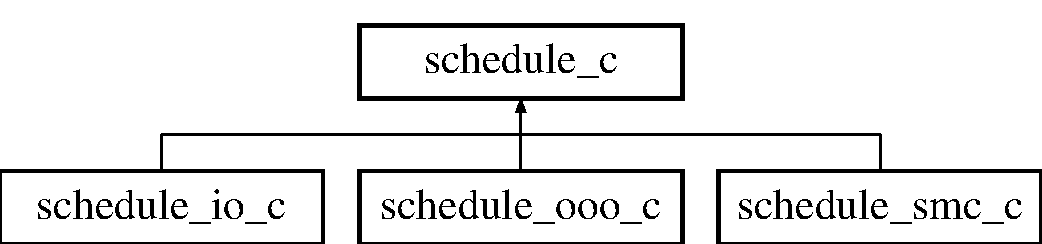
\includegraphics[height=2.000000cm]{classschedule__c}
\end{center}
\end{figure}
\subsection*{Public Member Functions}
\begin{DoxyCompactItemize}
\item 
\hyperlink{classschedule__c_aca30dd581b8b83035a0dc1ac13ae9f62}{schedule\_\-c} (\hyperlink{classexec__c}{exec\_\-c} $\ast$exec, int core\_\-id, Unit\_\-Type unit\_\-type, \hyperlink{classfrontend__c}{frontend\_\-c} $\ast$frontend, \hyperlink{classpqueue__c}{pqueue\_\-c}$<$ int $>$ $\ast$$\ast$alloc\_\-q, \hyperlink{classmacsim__c}{macsim\_\-c} $\ast$simBase)
\item 
virtual \hyperlink{classschedule__c_af8ea8faedf8812fb81810a208a3ad6cf}{$\sim$schedule\_\-c} ()
\item 
virtual void \hyperlink{classschedule__c_abaede0d6b5e70e5cfc6bf98801e387e1}{run\_\-a\_\-cycle} (void)=0
\item 
virtual void \hyperlink{classschedule__c_adbe783f74e34b8e1ae8f7ac707027509}{start} (void)
\begin{DoxyCompactList}\small\item\em Function to indicate the starting of the scheduler. \item\end{DoxyCompactList}\item 
virtual void \hyperlink{classschedule__c_a74262e51e68728870ac6de946c7d5e26}{stop} (void)
\begin{DoxyCompactList}\small\item\em Function to indicate the stopping of the scheduler. \item\end{DoxyCompactList}\item 
virtual bool \hyperlink{classschedule__c_a312b15c603395d8b36a1a1edb4838e70}{is\_\-running} (void)
\begin{DoxyCompactList}\small\item\em Function to check if the simulator is running. \item\end{DoxyCompactList}\item 
\hyperlink{classschedule__c_a2c5db70590e04fdb212b96aaa719a7ec}{schedule\_\-c} ()
\end{DoxyCompactItemize}
\subsection*{Protected Member Functions}
\begin{DoxyCompactItemize}
\item 
virtual bool \hyperlink{classschedule__c_a011e59bfd10373a4aaefec4c12a533de}{check\_\-srcs} (int entry)
\begin{DoxyCompactList}\small\item\em Function to check if the source of an uop are yet tp be scheduled. \item\end{DoxyCompactList}\item 
virtual bool \hyperlink{classschedule__c_a62bd97881f5ec86cee27a80b25b87ba9}{uop\_\-schedule} (int entry, SCHED\_\-FAIL\_\-TYPE $\ast$sched\_\-fail\_\-reason)
\begin{DoxyCompactList}\small\item\em Function to schedule uops. \item\end{DoxyCompactList}\item 
virtual void \hyperlink{classschedule__c_a35f2f1ea49453967c863c5de1acae87e}{advance} (int ALLOCQ\_\-index)
\begin{DoxyCompactList}\small\item\em Function to move the allocation queue ahead. \item\end{DoxyCompactList}\end{DoxyCompactItemize}
\subsection*{Protected Attributes}
\begin{DoxyCompactItemize}
\item 
int \hyperlink{classschedule__c_a6c4f8484b3f2dae8255c0ce064f9d46e}{m\_\-core\_\-id}
\item 
\hyperlink{classpqueue__c}{pqueue\_\-c}$<$ int $>$ $\ast$$\ast$ \hyperlink{classschedule__c_a54abfd4e67cf5e137e5f47ce52e8d903}{m\_\-alloc\_\-q}
\item 
\hyperlink{classrob__c}{rob\_\-c} $\ast$ \hyperlink{classschedule__c_a440a3a31b8fd41afae103a4b0ed3f49c}{m\_\-rob}
\item 
\hyperlink{classexec__c}{exec\_\-c} $\ast$ \hyperlink{classschedule__c_a75e32c0fe0d1ad336ada30787fceafd8}{m\_\-exec}
\item 
Unit\_\-Type \hyperlink{classschedule__c_a5fd7913b69e838b56da18de2802d8a71}{m\_\-unit\_\-type}
\item 
\hyperlink{classfrontend__c}{frontend\_\-c} $\ast$ \hyperlink{classschedule__c_a88ee09e9569c248374f0c943a4b73987}{m\_\-frontend}
\item 
Counter \hyperlink{classschedule__c_af4317f5116645b5847cef02ec5b6491c}{m\_\-cur\_\-core\_\-cycle}
\item 
uns16 \hyperlink{classschedule__c_a64a19cfe161bf6e7833bb8133849da67}{m\_\-knob\_\-width}
\item 
int \hyperlink{classschedule__c_a28362ea19de72375832f204b8d447237}{m\_\-num\_\-in\_\-sched}
\item 
bool \hyperlink{classschedule__c_a70ea92418d7c7b8e26a10c187ec0f57e}{m\_\-schedule\_\-running}
\item 
int \hyperlink{classschedule__c_a0dc86a2612108d557b5d9b4147b93a84}{m\_\-count} \mbox{[}max\_\-ALLOCQ\mbox{]}
\item 
int $\ast$ \hyperlink{classschedule__c_a3d8d6881abaa41ccccf6f173a23cc2bd}{m\_\-sched\_\-size}
\item 
int $\ast$ \hyperlink{classschedule__c_a04f5ccf337d6b385a6c50ed669343096}{m\_\-sched\_\-rate}
\item 
int $\ast$ \hyperlink{classschedule__c_a38b31f54c703cfde77a130c7a0cf2b9d}{m\_\-num\_\-per\_\-sched}
\item 
int \hyperlink{classschedule__c_adf653bc23f928cd4bed7db1200b53483}{m\_\-schedule\_\-list} \mbox{[}\hyperlink{classschedule__c_a1421dabfdead10b493bab949d79c2855}{MAX\_\-SCHED\_\-SIZE}\mbox{]}
\item 
int \hyperlink{classschedule__c_aa8a352d3017c16bf63d36ec12541238d}{m\_\-first\_\-schlist\_\-ptr}
\item 
int \hyperlink{classschedule__c_abfdb3ae734434b3a86c2402cf3d7e22c}{m\_\-last\_\-schlist\_\-ptr}
\item 
uns16 \hyperlink{classschedule__c_a92d6480db2a509909d356fc6b10d5d73}{m\_\-knob\_\-sched\_\-to\_\-width}
\item 
\hyperlink{classmacsim__c}{macsim\_\-c} $\ast$ \hyperlink{classschedule__c_a0db71234050b2c33f454b5d65d458564}{m\_\-simBase}
\end{DoxyCompactItemize}
\subsection*{Static Protected Attributes}
\begin{DoxyCompactItemize}
\item 
static const int \hyperlink{classschedule__c_a1421dabfdead10b493bab949d79c2855}{MAX\_\-SCHED\_\-SIZE} = 8192
\end{DoxyCompactItemize}


\subsection{Detailed Description}
Instruction scheduler base class. 

\subsection{Constructor \& Destructor Documentation}
\hypertarget{classschedule__c_aca30dd581b8b83035a0dc1ac13ae9f62}{
\index{schedule\_\-c@{schedule\_\-c}!schedule\_\-c@{schedule\_\-c}}
\index{schedule\_\-c@{schedule\_\-c}!schedule_c@{schedule\_\-c}}
\subsubsection[{schedule\_\-c}]{\setlength{\rightskip}{0pt plus 5cm}schedule\_\-c::schedule\_\-c (
\begin{DoxyParamCaption}
\item[{{\bf exec\_\-c} $\ast$}]{ exec, }
\item[{int}]{ core\_\-id, }
\item[{Unit\_\-Type}]{ unit\_\-type, }
\item[{{\bf frontend\_\-c} $\ast$}]{ frontend, }
\item[{{\bf pqueue\_\-c}$<$ int $>$ $\ast$$\ast$}]{ alloc\_\-q, }
\item[{{\bf macsim\_\-c} $\ast$}]{ simBase}
\end{DoxyParamCaption}
)}}
\label{classschedule__c_aca30dd581b8b83035a0dc1ac13ae9f62}
Constructor \hypertarget{classschedule__c_af8ea8faedf8812fb81810a208a3ad6cf}{
\index{schedule\_\-c@{schedule\_\-c}!$\sim$schedule\_\-c@{$\sim$schedule\_\-c}}
\index{$\sim$schedule\_\-c@{$\sim$schedule\_\-c}!schedule_c@{schedule\_\-c}}
\subsubsection[{$\sim$schedule\_\-c}]{\setlength{\rightskip}{0pt plus 5cm}schedule\_\-c::$\sim$schedule\_\-c (
\begin{DoxyParamCaption}
{}
\end{DoxyParamCaption}
)\hspace{0.3cm}{\ttfamily  \mbox{[}virtual\mbox{]}}}}
\label{classschedule__c_af8ea8faedf8812fb81810a208a3ad6cf}
Destructor \hypertarget{classschedule__c_a2c5db70590e04fdb212b96aaa719a7ec}{
\index{schedule\_\-c@{schedule\_\-c}!schedule\_\-c@{schedule\_\-c}}
\index{schedule\_\-c@{schedule\_\-c}!schedule_c@{schedule\_\-c}}
\subsubsection[{schedule\_\-c}]{\setlength{\rightskip}{0pt plus 5cm}schedule\_\-c::schedule\_\-c (
\begin{DoxyParamCaption}
{}
\end{DoxyParamCaption}
)}}
\label{classschedule__c_a2c5db70590e04fdb212b96aaa719a7ec}
Private constructor 

\subsection{Member Function Documentation}
\hypertarget{classschedule__c_a35f2f1ea49453967c863c5de1acae87e}{
\index{schedule\_\-c@{schedule\_\-c}!advance@{advance}}
\index{advance@{advance}!schedule_c@{schedule\_\-c}}
\subsubsection[{advance}]{\setlength{\rightskip}{0pt plus 5cm}void schedule\_\-c::advance (
\begin{DoxyParamCaption}
\item[{int}]{ ALLOCQ\_\-index}
\end{DoxyParamCaption}
)\hspace{0.3cm}{\ttfamily  \mbox{[}protected, virtual\mbox{]}}}}
\label{classschedule__c_a35f2f1ea49453967c863c5de1acae87e}


Function to move the allocation queue ahead. 


\begin{DoxyParams}{Parameters}
\item[{\em ALLOCQ\_\-index}]-\/ Aloocation queue number to be moved ahead \end{DoxyParams}
\begin{DoxyReturn}{Returns}
void 
\end{DoxyReturn}


Reimplemented in \hyperlink{classschedule__smc__c_a7f3ddbde213ee0afe9ba6af280bd6410}{schedule\_\-smc\_\-c}.

\hypertarget{classschedule__c_a011e59bfd10373a4aaefec4c12a533de}{
\index{schedule\_\-c@{schedule\_\-c}!check\_\-srcs@{check\_\-srcs}}
\index{check\_\-srcs@{check\_\-srcs}!schedule_c@{schedule\_\-c}}
\subsubsection[{check\_\-srcs}]{\setlength{\rightskip}{0pt plus 5cm}bool schedule\_\-c::check\_\-srcs (
\begin{DoxyParamCaption}
\item[{int}]{ entry}
\end{DoxyParamCaption}
)\hspace{0.3cm}{\ttfamily  \mbox{[}protected, virtual\mbox{]}}}}
\label{classschedule__c_a011e59bfd10373a4aaefec4c12a533de}


Function to check if the source of an uop are yet tp be scheduled. 


\begin{DoxyParams}{Parameters}
\item[{\em entry}]-\/ ROB entry of the uop \end{DoxyParams}
\begin{DoxyReturn}{Returns}
bool -\/ True if no dependency found 
\end{DoxyReturn}
\hypertarget{classschedule__c_a312b15c603395d8b36a1a1edb4838e70}{
\index{schedule\_\-c@{schedule\_\-c}!is\_\-running@{is\_\-running}}
\index{is\_\-running@{is\_\-running}!schedule_c@{schedule\_\-c}}
\subsubsection[{is\_\-running}]{\setlength{\rightskip}{0pt plus 5cm}void schedule\_\-c::is\_\-running (
\begin{DoxyParamCaption}
\item[{void}]{}
\end{DoxyParamCaption}
)\hspace{0.3cm}{\ttfamily  \mbox{[}virtual\mbox{]}}}}
\label{classschedule__c_a312b15c603395d8b36a1a1edb4838e70}


Function to check if the simulator is running. 

\begin{DoxyReturn}{Returns}
void 
\end{DoxyReturn}
\hypertarget{classschedule__c_abaede0d6b5e70e5cfc6bf98801e387e1}{
\index{schedule\_\-c@{schedule\_\-c}!run\_\-a\_\-cycle@{run\_\-a\_\-cycle}}
\index{run\_\-a\_\-cycle@{run\_\-a\_\-cycle}!schedule_c@{schedule\_\-c}}
\subsubsection[{run\_\-a\_\-cycle}]{\setlength{\rightskip}{0pt plus 5cm}virtual void schedule\_\-c::run\_\-a\_\-cycle (
\begin{DoxyParamCaption}
\item[{void}]{}
\end{DoxyParamCaption}
)\hspace{0.3cm}{\ttfamily  \mbox{[}pure virtual\mbox{]}}}}
\label{classschedule__c_abaede0d6b5e70e5cfc6bf98801e387e1}
Tick a cycle 

Implemented in \hyperlink{classschedule__io__c_add1ff393e65774fabedc6b4069793c9f}{schedule\_\-io\_\-c}, \hyperlink{classschedule__ooo__c_ae5d87735e3c75bca820797d8185f2dad}{schedule\_\-ooo\_\-c}, and \hyperlink{classschedule__smc__c_aeb80c4988ef300b7dbd8f54fadc1a2ae}{schedule\_\-smc\_\-c}.

\hypertarget{classschedule__c_adbe783f74e34b8e1ae8f7ac707027509}{
\index{schedule\_\-c@{schedule\_\-c}!start@{start}}
\index{start@{start}!schedule_c@{schedule\_\-c}}
\subsubsection[{start}]{\setlength{\rightskip}{0pt plus 5cm}void schedule\_\-c::start (
\begin{DoxyParamCaption}
\item[{void}]{}
\end{DoxyParamCaption}
)\hspace{0.3cm}{\ttfamily  \mbox{[}virtual\mbox{]}}}}
\label{classschedule__c_adbe783f74e34b8e1ae8f7ac707027509}


Function to indicate the starting of the scheduler. 

\begin{DoxyReturn}{Returns}
void 
\end{DoxyReturn}
\hypertarget{classschedule__c_a74262e51e68728870ac6de946c7d5e26}{
\index{schedule\_\-c@{schedule\_\-c}!stop@{stop}}
\index{stop@{stop}!schedule_c@{schedule\_\-c}}
\subsubsection[{stop}]{\setlength{\rightskip}{0pt plus 5cm}void schedule\_\-c::stop (
\begin{DoxyParamCaption}
\item[{void}]{}
\end{DoxyParamCaption}
)\hspace{0.3cm}{\ttfamily  \mbox{[}virtual\mbox{]}}}}
\label{classschedule__c_a74262e51e68728870ac6de946c7d5e26}


Function to indicate the stopping of the scheduler. 

\begin{DoxyReturn}{Returns}
void 
\end{DoxyReturn}
\hypertarget{classschedule__c_a62bd97881f5ec86cee27a80b25b87ba9}{
\index{schedule\_\-c@{schedule\_\-c}!uop\_\-schedule@{uop\_\-schedule}}
\index{uop\_\-schedule@{uop\_\-schedule}!schedule_c@{schedule\_\-c}}
\subsubsection[{uop\_\-schedule}]{\setlength{\rightskip}{0pt plus 5cm}bool schedule\_\-c::uop\_\-schedule (
\begin{DoxyParamCaption}
\item[{int}]{ entry, }
\item[{SCHED\_\-FAIL\_\-TYPE $\ast$}]{ sched\_\-fail\_\-reason}
\end{DoxyParamCaption}
)\hspace{0.3cm}{\ttfamily  \mbox{[}protected, virtual\mbox{]}}}}
\label{classschedule__c_a62bd97881f5ec86cee27a80b25b87ba9}


Function to schedule uops. 


\begin{DoxyParams}{Parameters}
\item[{\em entry}]-\/ ROB entry of the uop \item[{\em sched\_\-fail\_\-reason}]-\/ Reason of uop schedule failure \end{DoxyParams}
\begin{DoxyReturn}{Returns}
bool -\/ True on success in scheduling 
\end{DoxyReturn}


\subsection{Member Data Documentation}
\hypertarget{classschedule__c_a54abfd4e67cf5e137e5f47ce52e8d903}{
\index{schedule\_\-c@{schedule\_\-c}!m\_\-alloc\_\-q@{m\_\-alloc\_\-q}}
\index{m\_\-alloc\_\-q@{m\_\-alloc\_\-q}!schedule_c@{schedule\_\-c}}
\subsubsection[{m\_\-alloc\_\-q}]{\setlength{\rightskip}{0pt plus 5cm}{\bf pqueue\_\-c}$<$int$>$$\ast$$\ast$ {\bf schedule\_\-c::m\_\-alloc\_\-q}\hspace{0.3cm}{\ttfamily  \mbox{[}protected\mbox{]}}}}
\label{classschedule__c_a54abfd4e67cf5e137e5f47ce52e8d903}
allocation queue \hypertarget{classschedule__c_a6c4f8484b3f2dae8255c0ce064f9d46e}{
\index{schedule\_\-c@{schedule\_\-c}!m\_\-core\_\-id@{m\_\-core\_\-id}}
\index{m\_\-core\_\-id@{m\_\-core\_\-id}!schedule_c@{schedule\_\-c}}
\subsubsection[{m\_\-core\_\-id}]{\setlength{\rightskip}{0pt plus 5cm}int {\bf schedule\_\-c::m\_\-core\_\-id}\hspace{0.3cm}{\ttfamily  \mbox{[}protected\mbox{]}}}}
\label{classschedule__c_a6c4f8484b3f2dae8255c0ce064f9d46e}
core id \hypertarget{classschedule__c_a0dc86a2612108d557b5d9b4147b93a84}{
\index{schedule\_\-c@{schedule\_\-c}!m\_\-count@{m\_\-count}}
\index{m\_\-count@{m\_\-count}!schedule_c@{schedule\_\-c}}
\subsubsection[{m\_\-count}]{\setlength{\rightskip}{0pt plus 5cm}int {\bf schedule\_\-c::m\_\-count}\mbox{[}max\_\-ALLOCQ\mbox{]}\hspace{0.3cm}{\ttfamily  \mbox{[}protected\mbox{]}}}}
\label{classschedule__c_a0dc86a2612108d557b5d9b4147b93a84}
total scheduled uop \hypertarget{classschedule__c_af4317f5116645b5847cef02ec5b6491c}{
\index{schedule\_\-c@{schedule\_\-c}!m\_\-cur\_\-core\_\-cycle@{m\_\-cur\_\-core\_\-cycle}}
\index{m\_\-cur\_\-core\_\-cycle@{m\_\-cur\_\-core\_\-cycle}!schedule_c@{schedule\_\-c}}
\subsubsection[{m\_\-cur\_\-core\_\-cycle}]{\setlength{\rightskip}{0pt plus 5cm}Counter {\bf schedule\_\-c::m\_\-cur\_\-core\_\-cycle}\hspace{0.3cm}{\ttfamily  \mbox{[}protected\mbox{]}}}}
\label{classschedule__c_af4317f5116645b5847cef02ec5b6491c}
current core cycle \hypertarget{classschedule__c_a75e32c0fe0d1ad336ada30787fceafd8}{
\index{schedule\_\-c@{schedule\_\-c}!m\_\-exec@{m\_\-exec}}
\index{m\_\-exec@{m\_\-exec}!schedule_c@{schedule\_\-c}}
\subsubsection[{m\_\-exec}]{\setlength{\rightskip}{0pt plus 5cm}{\bf exec\_\-c}$\ast$ {\bf schedule\_\-c::m\_\-exec}\hspace{0.3cm}{\ttfamily  \mbox{[}protected\mbox{]}}}}
\label{classschedule__c_a75e32c0fe0d1ad336ada30787fceafd8}
execution stage pointer \hypertarget{classschedule__c_aa8a352d3017c16bf63d36ec12541238d}{
\index{schedule\_\-c@{schedule\_\-c}!m\_\-first\_\-schlist\_\-ptr@{m\_\-first\_\-schlist\_\-ptr}}
\index{m\_\-first\_\-schlist\_\-ptr@{m\_\-first\_\-schlist\_\-ptr}!schedule_c@{schedule\_\-c}}
\subsubsection[{m\_\-first\_\-schlist\_\-ptr}]{\setlength{\rightskip}{0pt plus 5cm}int {\bf schedule\_\-c::m\_\-first\_\-schlist\_\-ptr}\hspace{0.3cm}{\ttfamily  \mbox{[}protected\mbox{]}}}}
\label{classschedule__c_aa8a352d3017c16bf63d36ec12541238d}
first index to sched list in OOO \hypertarget{classschedule__c_a88ee09e9569c248374f0c943a4b73987}{
\index{schedule\_\-c@{schedule\_\-c}!m\_\-frontend@{m\_\-frontend}}
\index{m\_\-frontend@{m\_\-frontend}!schedule_c@{schedule\_\-c}}
\subsubsection[{m\_\-frontend}]{\setlength{\rightskip}{0pt plus 5cm}{\bf frontend\_\-c}$\ast$ {\bf schedule\_\-c::m\_\-frontend}\hspace{0.3cm}{\ttfamily  \mbox{[}protected\mbox{]}}}}
\label{classschedule__c_a88ee09e9569c248374f0c943a4b73987}
frontend pointer \hypertarget{classschedule__c_a92d6480db2a509909d356fc6b10d5d73}{
\index{schedule\_\-c@{schedule\_\-c}!m\_\-knob\_\-sched\_\-to\_\-width@{m\_\-knob\_\-sched\_\-to\_\-width}}
\index{m\_\-knob\_\-sched\_\-to\_\-width@{m\_\-knob\_\-sched\_\-to\_\-width}!schedule_c@{schedule\_\-c}}
\subsubsection[{m\_\-knob\_\-sched\_\-to\_\-width}]{\setlength{\rightskip}{0pt plus 5cm}uns16 {\bf schedule\_\-c::m\_\-knob\_\-sched\_\-to\_\-width}\hspace{0.3cm}{\ttfamily  \mbox{[}protected\mbox{]}}}}
\label{classschedule__c_a92d6480db2a509909d356fc6b10d5d73}
knob sched to width FIXME \hypertarget{classschedule__c_a64a19cfe161bf6e7833bb8133849da67}{
\index{schedule\_\-c@{schedule\_\-c}!m\_\-knob\_\-width@{m\_\-knob\_\-width}}
\index{m\_\-knob\_\-width@{m\_\-knob\_\-width}!schedule_c@{schedule\_\-c}}
\subsubsection[{m\_\-knob\_\-width}]{\setlength{\rightskip}{0pt plus 5cm}uns16 {\bf schedule\_\-c::m\_\-knob\_\-width}\hspace{0.3cm}{\ttfamily  \mbox{[}protected\mbox{]}}}}
\label{classschedule__c_a64a19cfe161bf6e7833bb8133849da67}
width \hypertarget{classschedule__c_abfdb3ae734434b3a86c2402cf3d7e22c}{
\index{schedule\_\-c@{schedule\_\-c}!m\_\-last\_\-schlist\_\-ptr@{m\_\-last\_\-schlist\_\-ptr}}
\index{m\_\-last\_\-schlist\_\-ptr@{m\_\-last\_\-schlist\_\-ptr}!schedule_c@{schedule\_\-c}}
\subsubsection[{m\_\-last\_\-schlist\_\-ptr}]{\setlength{\rightskip}{0pt plus 5cm}int {\bf schedule\_\-c::m\_\-last\_\-schlist\_\-ptr}\hspace{0.3cm}{\ttfamily  \mbox{[}protected\mbox{]}}}}
\label{classschedule__c_abfdb3ae734434b3a86c2402cf3d7e22c}
last index to sched list in OOO \hypertarget{classschedule__c_a28362ea19de72375832f204b8d447237}{
\index{schedule\_\-c@{schedule\_\-c}!m\_\-num\_\-in\_\-sched@{m\_\-num\_\-in\_\-sched}}
\index{m\_\-num\_\-in\_\-sched@{m\_\-num\_\-in\_\-sched}!schedule_c@{schedule\_\-c}}
\subsubsection[{m\_\-num\_\-in\_\-sched}]{\setlength{\rightskip}{0pt plus 5cm}int {\bf schedule\_\-c::m\_\-num\_\-in\_\-sched}\hspace{0.3cm}{\ttfamily  \mbox{[}protected\mbox{]}}}}
\label{classschedule__c_a28362ea19de72375832f204b8d447237}
number of uops in scheduler \hypertarget{classschedule__c_a38b31f54c703cfde77a130c7a0cf2b9d}{
\index{schedule\_\-c@{schedule\_\-c}!m\_\-num\_\-per\_\-sched@{m\_\-num\_\-per\_\-sched}}
\index{m\_\-num\_\-per\_\-sched@{m\_\-num\_\-per\_\-sched}!schedule_c@{schedule\_\-c}}
\subsubsection[{m\_\-num\_\-per\_\-sched}]{\setlength{\rightskip}{0pt plus 5cm}int$\ast$ {\bf schedule\_\-c::m\_\-num\_\-per\_\-sched}\hspace{0.3cm}{\ttfamily  \mbox{[}protected\mbox{]}}}}
\label{classschedule__c_a38b31f54c703cfde77a130c7a0cf2b9d}
number of uops in each sched. \hypertarget{classschedule__c_a440a3a31b8fd41afae103a4b0ed3f49c}{
\index{schedule\_\-c@{schedule\_\-c}!m\_\-rob@{m\_\-rob}}
\index{m\_\-rob@{m\_\-rob}!schedule_c@{schedule\_\-c}}
\subsubsection[{m\_\-rob}]{\setlength{\rightskip}{0pt plus 5cm}{\bf rob\_\-c}$\ast$ {\bf schedule\_\-c::m\_\-rob}\hspace{0.3cm}{\ttfamily  \mbox{[}protected\mbox{]}}}}
\label{classschedule__c_a440a3a31b8fd41afae103a4b0ed3f49c}
reorder buffer \hypertarget{classschedule__c_a04f5ccf337d6b385a6c50ed669343096}{
\index{schedule\_\-c@{schedule\_\-c}!m\_\-sched\_\-rate@{m\_\-sched\_\-rate}}
\index{m\_\-sched\_\-rate@{m\_\-sched\_\-rate}!schedule_c@{schedule\_\-c}}
\subsubsection[{m\_\-sched\_\-rate}]{\setlength{\rightskip}{0pt plus 5cm}int$\ast$ {\bf schedule\_\-c::m\_\-sched\_\-rate}\hspace{0.3cm}{\ttfamily  \mbox{[}protected\mbox{]}}}}
\label{classschedule__c_a04f5ccf337d6b385a6c50ed669343096}
schedule rate per inst. type \hypertarget{classschedule__c_a3d8d6881abaa41ccccf6f173a23cc2bd}{
\index{schedule\_\-c@{schedule\_\-c}!m\_\-sched\_\-size@{m\_\-sched\_\-size}}
\index{m\_\-sched\_\-size@{m\_\-sched\_\-size}!schedule_c@{schedule\_\-c}}
\subsubsection[{m\_\-sched\_\-size}]{\setlength{\rightskip}{0pt plus 5cm}int$\ast$ {\bf schedule\_\-c::m\_\-sched\_\-size}\hspace{0.3cm}{\ttfamily  \mbox{[}protected\mbox{]}}}}
\label{classschedule__c_a3d8d6881abaa41ccccf6f173a23cc2bd}
schedule size per inst. type \hypertarget{classschedule__c_adf653bc23f928cd4bed7db1200b53483}{
\index{schedule\_\-c@{schedule\_\-c}!m\_\-schedule\_\-list@{m\_\-schedule\_\-list}}
\index{m\_\-schedule\_\-list@{m\_\-schedule\_\-list}!schedule_c@{schedule\_\-c}}
\subsubsection[{m\_\-schedule\_\-list}]{\setlength{\rightskip}{0pt plus 5cm}int {\bf schedule\_\-c::m\_\-schedule\_\-list}\mbox{[}{\bf MAX\_\-SCHED\_\-SIZE}\mbox{]}\hspace{0.3cm}{\ttfamily  \mbox{[}protected\mbox{]}}}}
\label{classschedule__c_adf653bc23f928cd4bed7db1200b53483}
schedule list in OOO \hypertarget{classschedule__c_a70ea92418d7c7b8e26a10c187ec0f57e}{
\index{schedule\_\-c@{schedule\_\-c}!m\_\-schedule\_\-running@{m\_\-schedule\_\-running}}
\index{m\_\-schedule\_\-running@{m\_\-schedule\_\-running}!schedule_c@{schedule\_\-c}}
\subsubsection[{m\_\-schedule\_\-running}]{\setlength{\rightskip}{0pt plus 5cm}bool {\bf schedule\_\-c::m\_\-schedule\_\-running}\hspace{0.3cm}{\ttfamily  \mbox{[}protected\mbox{]}}}}
\label{classschedule__c_a70ea92418d7c7b8e26a10c187ec0f57e}
enabled scheduler \hypertarget{classschedule__c_a0db71234050b2c33f454b5d65d458564}{
\index{schedule\_\-c@{schedule\_\-c}!m\_\-simBase@{m\_\-simBase}}
\index{m\_\-simBase@{m\_\-simBase}!schedule_c@{schedule\_\-c}}
\subsubsection[{m\_\-simBase}]{\setlength{\rightskip}{0pt plus 5cm}{\bf macsim\_\-c}$\ast$ {\bf schedule\_\-c::m\_\-simBase}\hspace{0.3cm}{\ttfamily  \mbox{[}protected\mbox{]}}}}
\label{classschedule__c_a0db71234050b2c33f454b5d65d458564}
\hyperlink{classmacsim__c}{macsim\_\-c} base class for simulation globals 

Reimplemented in \hyperlink{classschedule__io__c_a4fd792581e727219c93a1d4ac6707cbd}{schedule\_\-io\_\-c}, \hyperlink{classschedule__ooo__c_a0b06680167ffaa41d348215de2144d29}{schedule\_\-ooo\_\-c}, and \hyperlink{classschedule__smc__c_a40d5c66331f8f72123691ebbb4590f3b}{schedule\_\-smc\_\-c}.

\hypertarget{classschedule__c_a5fd7913b69e838b56da18de2802d8a71}{
\index{schedule\_\-c@{schedule\_\-c}!m\_\-unit\_\-type@{m\_\-unit\_\-type}}
\index{m\_\-unit\_\-type@{m\_\-unit\_\-type}!schedule_c@{schedule\_\-c}}
\subsubsection[{m\_\-unit\_\-type}]{\setlength{\rightskip}{0pt plus 5cm}Unit\_\-Type {\bf schedule\_\-c::m\_\-unit\_\-type}\hspace{0.3cm}{\ttfamily  \mbox{[}protected\mbox{]}}}}
\label{classschedule__c_a5fd7913b69e838b56da18de2802d8a71}
core type \hypertarget{classschedule__c_a1421dabfdead10b493bab949d79c2855}{
\index{schedule\_\-c@{schedule\_\-c}!MAX\_\-SCHED\_\-SIZE@{MAX\_\-SCHED\_\-SIZE}}
\index{MAX\_\-SCHED\_\-SIZE@{MAX\_\-SCHED\_\-SIZE}!schedule_c@{schedule\_\-c}}
\subsubsection[{MAX\_\-SCHED\_\-SIZE}]{\setlength{\rightskip}{0pt plus 5cm}const int {\bf schedule\_\-c::MAX\_\-SCHED\_\-SIZE} = 8192\hspace{0.3cm}{\ttfamily  \mbox{[}static, protected\mbox{]}}}}
\label{classschedule__c_a1421dabfdead10b493bab949d79c2855}
maximum scheduler table size 

The documentation for this class was generated from the following files:\begin{DoxyCompactItemize}
\item 
schedule.h\item 
schedule.cc\end{DoxyCompactItemize}

\hypertarget{classschedule__io__c}{
\section{schedule\_\-io\_\-c Class Reference}
\label{classschedule__io__c}\index{schedule\_\-io\_\-c@{schedule\_\-io\_\-c}}
}


In-\/order scheduler class.  




{\ttfamily \#include $<$schedule\_\-io.h$>$}

Inheritance diagram for schedule\_\-io\_\-c:\begin{figure}[H]
\begin{center}
\leavevmode
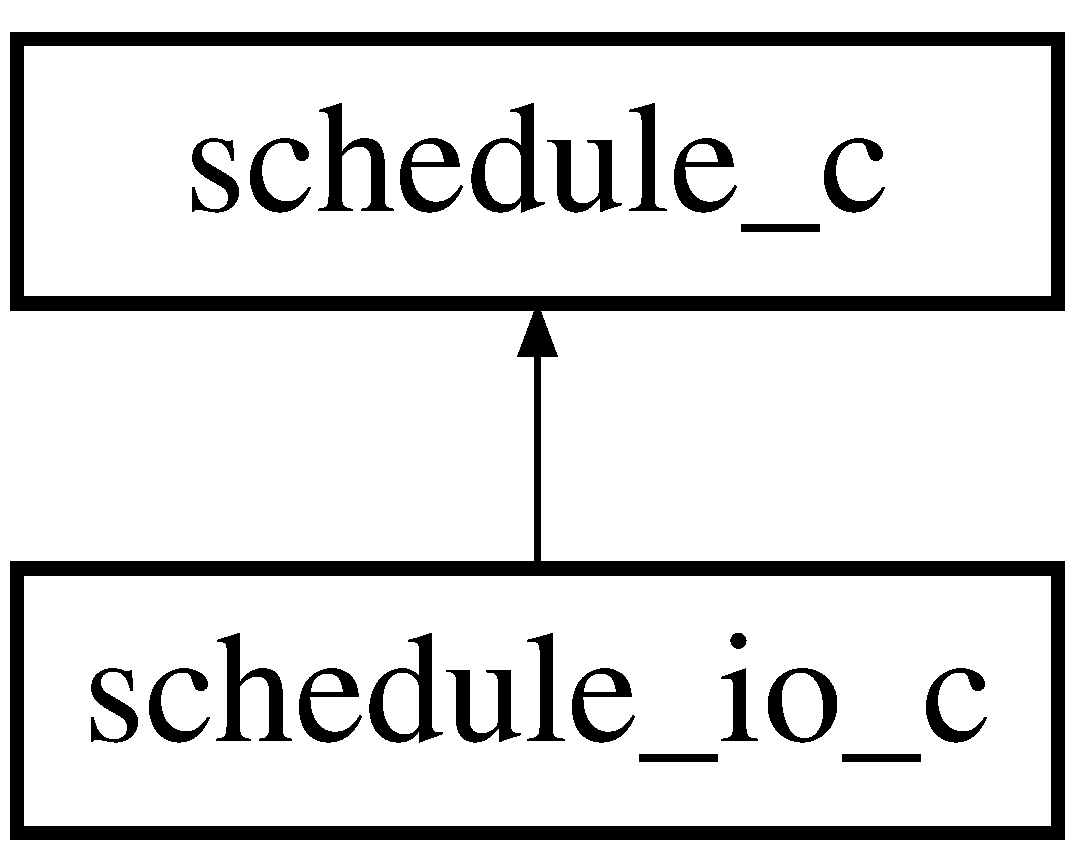
\includegraphics[height=2.000000cm]{classschedule__io__c}
\end{center}
\end{figure}
\subsection*{Public Member Functions}
\begin{DoxyCompactItemize}
\item 
\hyperlink{classschedule__io__c_a57961ab7add32f6e032e7ed03cd37442}{schedule\_\-io\_\-c} (int \hyperlink{classschedule__c_a6c4f8484b3f2dae8255c0ce064f9d46e}{m\_\-core\_\-id}, \hyperlink{classpqueue__c}{pqueue\_\-c}$<$ int $>$ $\ast$$\ast$\hyperlink{classschedule__c_a54abfd4e67cf5e137e5f47ce52e8d903}{m\_\-alloc\_\-q}, \hyperlink{classrob__c}{rob\_\-c} $\ast$\hyperlink{classschedule__c_a440a3a31b8fd41afae103a4b0ed3f49c}{m\_\-rob}, \hyperlink{classexec__c}{exec\_\-c} $\ast$\hyperlink{classschedule__c_a75e32c0fe0d1ad336ada30787fceafd8}{m\_\-exec}, Unit\_\-Type \hyperlink{classschedule__c_a5fd7913b69e838b56da18de2802d8a71}{m\_\-unit\_\-type}, \hyperlink{classfrontend__c}{frontend\_\-c} $\ast$\hyperlink{classschedule__c_a88ee09e9569c248374f0c943a4b73987}{m\_\-frontend}, \hyperlink{classmacsim__c}{macsim\_\-c} $\ast$simBase)
\begin{DoxyCompactList}\small\item\em Constructor for the Inorder scheluder class. \item\end{DoxyCompactList}\item 
\hyperlink{classschedule__io__c_a1dd49046b8bc3795f66cd60c2eefff7f}{$\sim$schedule\_\-io\_\-c} ()
\begin{DoxyCompactList}\small\item\em Destructor for the Inorder scheduler. \item\end{DoxyCompactList}\item 
void \hyperlink{classschedule__io__c_add1ff393e65774fabedc6b4069793c9f}{run\_\-a\_\-cycle} ()
\begin{DoxyCompactList}\small\item\em Function to perform the activities of a cycle for the scheduler. \item\end{DoxyCompactList}\end{DoxyCompactItemize}
\subsection*{Private Attributes}
\begin{DoxyCompactItemize}
\item 
int \hyperlink{classschedule__io__c_a5bf81c5205db201ff80eb9d99da075a3}{m\_\-next\_\-inorder\_\-to\_\-schedule}
\item 
\hyperlink{classmacsim__c}{macsim\_\-c} $\ast$ \hyperlink{classschedule__io__c_a4fd792581e727219c93a1d4ac6707cbd}{m\_\-simBase}
\end{DoxyCompactItemize}


\subsection{Detailed Description}
In-\/order scheduler class. 

\subsection{Constructor \& Destructor Documentation}
\hypertarget{classschedule__io__c_a57961ab7add32f6e032e7ed03cd37442}{
\index{schedule\_\-io\_\-c@{schedule\_\-io\_\-c}!schedule\_\-io\_\-c@{schedule\_\-io\_\-c}}
\index{schedule\_\-io\_\-c@{schedule\_\-io\_\-c}!schedule_io_c@{schedule\_\-io\_\-c}}
\subsubsection[{schedule\_\-io\_\-c}]{\setlength{\rightskip}{0pt plus 5cm}schedule\_\-io\_\-c::schedule\_\-io\_\-c (
\begin{DoxyParamCaption}
\item[{int}]{ m\_\-core\_\-id, }
\item[{{\bf pqueue\_\-c}$<$ int $>$ $\ast$$\ast$}]{ m\_\-alloc\_\-q, }
\item[{{\bf rob\_\-c} $\ast$}]{ m\_\-rob, }
\item[{{\bf exec\_\-c} $\ast$}]{ m\_\-exec, }
\item[{Unit\_\-Type}]{ m\_\-unit\_\-type, }
\item[{{\bf frontend\_\-c} $\ast$}]{ m\_\-frontend, }
\item[{{\bf macsim\_\-c} $\ast$}]{ simBase}
\end{DoxyParamCaption}
)}}
\label{classschedule__io__c_a57961ab7add32f6e032e7ed03cd37442}


Constructor for the Inorder scheluder class. 


\begin{DoxyParams}{Parameters}
\item[{\em m\_\-core\_\-id}]-\/ Core identifier number \item[{\em m\_\-alloc\_\-q}]-\/ Pointer to be updated with the allocation stage queue \item[{\em m\_\-rob}]-\/ Pointer to the Reorder buffer \item[{\em m\_\-exec}]-\/ Pointer to m\_\-execution unit \item[{\em m\_\-unit\_\-type}]-\/ Parameter used to identify knob width \item[{\em m\_\-frontend}]-\/ Pointer to front end queue \end{DoxyParams}
\begin{DoxyReturn}{Returns}
void 
\end{DoxyReturn}
\hypertarget{classschedule__io__c_a1dd49046b8bc3795f66cd60c2eefff7f}{
\index{schedule\_\-io\_\-c@{schedule\_\-io\_\-c}!$\sim$schedule\_\-io\_\-c@{$\sim$schedule\_\-io\_\-c}}
\index{$\sim$schedule\_\-io\_\-c@{$\sim$schedule\_\-io\_\-c}!schedule_io_c@{schedule\_\-io\_\-c}}
\subsubsection[{$\sim$schedule\_\-io\_\-c}]{\setlength{\rightskip}{0pt plus 5cm}schedule\_\-io\_\-c::$\sim$schedule\_\-io\_\-c (
\begin{DoxyParamCaption}
\item[{void}]{}
\end{DoxyParamCaption}
)}}
\label{classschedule__io__c_a1dd49046b8bc3795f66cd60c2eefff7f}


Destructor for the Inorder scheduler. 

\begin{DoxyReturn}{Returns}
void 
\end{DoxyReturn}


\subsection{Member Function Documentation}
\hypertarget{classschedule__io__c_add1ff393e65774fabedc6b4069793c9f}{
\index{schedule\_\-io\_\-c@{schedule\_\-io\_\-c}!run\_\-a\_\-cycle@{run\_\-a\_\-cycle}}
\index{run\_\-a\_\-cycle@{run\_\-a\_\-cycle}!schedule_io_c@{schedule\_\-io\_\-c}}
\subsubsection[{run\_\-a\_\-cycle}]{\setlength{\rightskip}{0pt plus 5cm}void schedule\_\-io\_\-c::run\_\-a\_\-cycle (
\begin{DoxyParamCaption}
\item[{void}]{}
\end{DoxyParamCaption}
)\hspace{0.3cm}{\ttfamily  \mbox{[}virtual\mbox{]}}}}
\label{classschedule__io__c_add1ff393e65774fabedc6b4069793c9f}


Function to perform the activities of a cycle for the scheduler. 

\begin{DoxyReturn}{Returns}
void 
\end{DoxyReturn}


Implements \hyperlink{classschedule__c_abaede0d6b5e70e5cfc6bf98801e387e1}{schedule\_\-c}.



\subsection{Member Data Documentation}
\hypertarget{classschedule__io__c_a5bf81c5205db201ff80eb9d99da075a3}{
\index{schedule\_\-io\_\-c@{schedule\_\-io\_\-c}!m\_\-next\_\-inorder\_\-to\_\-schedule@{m\_\-next\_\-inorder\_\-to\_\-schedule}}
\index{m\_\-next\_\-inorder\_\-to\_\-schedule@{m\_\-next\_\-inorder\_\-to\_\-schedule}!schedule_io_c@{schedule\_\-io\_\-c}}
\subsubsection[{m\_\-next\_\-inorder\_\-to\_\-schedule}]{\setlength{\rightskip}{0pt plus 5cm}int {\bf schedule\_\-io\_\-c::m\_\-next\_\-inorder\_\-to\_\-schedule}\hspace{0.3cm}{\ttfamily  \mbox{[}private\mbox{]}}}}
\label{classschedule__io__c_a5bf81c5205db201ff80eb9d99da075a3}
index to rob for next uop to schedule \hypertarget{classschedule__io__c_a4fd792581e727219c93a1d4ac6707cbd}{
\index{schedule\_\-io\_\-c@{schedule\_\-io\_\-c}!m\_\-simBase@{m\_\-simBase}}
\index{m\_\-simBase@{m\_\-simBase}!schedule_io_c@{schedule\_\-io\_\-c}}
\subsubsection[{m\_\-simBase}]{\setlength{\rightskip}{0pt plus 5cm}{\bf macsim\_\-c}$\ast$ {\bf schedule\_\-io\_\-c::m\_\-simBase}\hspace{0.3cm}{\ttfamily  \mbox{[}private\mbox{]}}}}
\label{classschedule__io__c_a4fd792581e727219c93a1d4ac6707cbd}
\hyperlink{classmacsim__c}{macsim\_\-c} base class for simulation globals 

Reimplemented from \hyperlink{classschedule__c_a0db71234050b2c33f454b5d65d458564}{schedule\_\-c}.



The documentation for this class was generated from the following files:\begin{DoxyCompactItemize}
\item 
schedule\_\-io.h\item 
schedule\_\-io.cc\end{DoxyCompactItemize}

\hypertarget{classschedule__ooo__c}{
\section{schedule\_\-ooo\_\-c Class Reference}
\label{classschedule__ooo__c}\index{schedule\_\-ooo\_\-c@{schedule\_\-ooo\_\-c}}
}


Out-\/of-\/order (OOO) scheduler.  




{\ttfamily \#include $<$schedule\_\-ooo.h$>$}

Inheritance diagram for schedule\_\-ooo\_\-c:\begin{figure}[H]
\begin{center}
\leavevmode
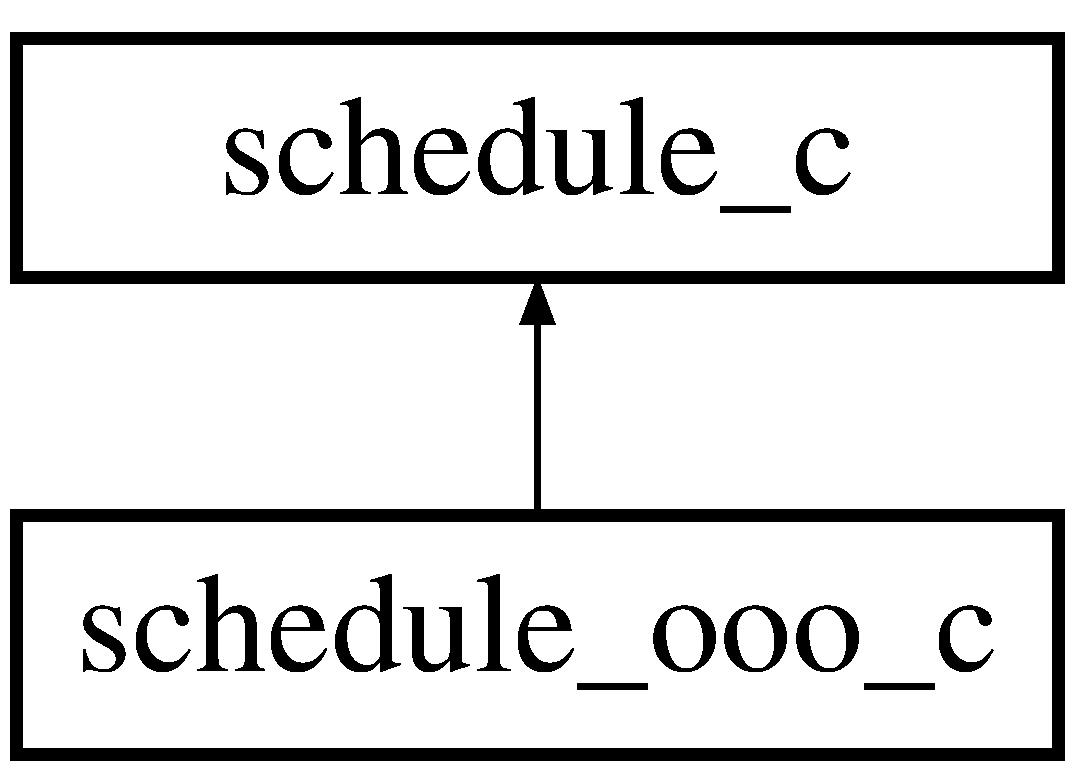
\includegraphics[height=2.000000cm]{classschedule__ooo__c}
\end{center}
\end{figure}
\subsection*{Public Member Functions}
\begin{DoxyCompactItemize}
\item 
\hyperlink{classschedule__ooo__c_aec8a55262e3319c9090fa8f4837bebbc}{schedule\_\-ooo\_\-c} (int core\_\-id, \hyperlink{classpqueue__c}{pqueue\_\-c}$<$ int $>$ $\ast$$\ast$q\_\-iaq, \hyperlink{classrob__c}{rob\_\-c} $\ast$rob, \hyperlink{classexec__c}{exec\_\-c} $\ast$exec, Unit\_\-Type unit\_\-type, \hyperlink{classfrontend__c}{frontend\_\-c} $\ast$frontend, \hyperlink{classmacsim__c}{macsim\_\-c} $\ast$simBase)
\begin{DoxyCompactList}\small\item\em Constructor for the Out of order scheluder class. \item\end{DoxyCompactList}\item 
\hyperlink{classschedule__ooo__c_a2bb8139f29bfd8c5958170e3bd869a9e}{$\sim$schedule\_\-ooo\_\-c} (void)
\begin{DoxyCompactList}\small\item\em Destructor for the Out of order scheduler. \item\end{DoxyCompactList}\item 
void \hyperlink{classschedule__ooo__c_ae5d87735e3c75bca820797d8185f2dad}{run\_\-a\_\-cycle} ()
\begin{DoxyCompactList}\small\item\em Function to perform the activities of a cycle for the scheduler. \item\end{DoxyCompactList}\end{DoxyCompactItemize}
\subsection*{Private Attributes}
\begin{DoxyCompactItemize}
\item 
\hyperlink{classmacsim__c}{macsim\_\-c} $\ast$ \hyperlink{classschedule__ooo__c_a0b06680167ffaa41d348215de2144d29}{m\_\-simBase}
\end{DoxyCompactItemize}


\subsection{Detailed Description}
Out-\/of-\/order (OOO) scheduler. 

\subsection{Constructor \& Destructor Documentation}
\hypertarget{classschedule__ooo__c_aec8a55262e3319c9090fa8f4837bebbc}{
\index{schedule\_\-ooo\_\-c@{schedule\_\-ooo\_\-c}!schedule\_\-ooo\_\-c@{schedule\_\-ooo\_\-c}}
\index{schedule\_\-ooo\_\-c@{schedule\_\-ooo\_\-c}!schedule_ooo_c@{schedule\_\-ooo\_\-c}}
\subsubsection[{schedule\_\-ooo\_\-c}]{\setlength{\rightskip}{0pt plus 5cm}schedule\_\-ooo\_\-c::schedule\_\-ooo\_\-c (
\begin{DoxyParamCaption}
\item[{int}]{ core\_\-id, }
\item[{{\bf pqueue\_\-c}$<$ int $>$ $\ast$$\ast$}]{ q\_\-iaq, }
\item[{{\bf rob\_\-c} $\ast$}]{ rob, }
\item[{{\bf exec\_\-c} $\ast$}]{ exec, }
\item[{Unit\_\-Type}]{ unit\_\-type, }
\item[{{\bf frontend\_\-c} $\ast$}]{ frontend, }
\item[{{\bf macsim\_\-c} $\ast$}]{ simBase}
\end{DoxyParamCaption}
)}}
\label{classschedule__ooo__c_aec8a55262e3319c9090fa8f4837bebbc}


Constructor for the Out of order scheluder class. 


\begin{DoxyParams}{Parameters}
\item[{\em core\_\-id}]-\/ Core identifier number \item[{\em q\_\-iaq}]-\/ Pointer to be updated with the allocation stage queue \item[{\em rob}]-\/ Pointer to the Reorder buffer \item[{\em exec}]-\/ Pointer to m\_\-execution unit \item[{\em unit\_\-type}]-\/ Parameter used to identify knob width \item[{\em frontend}]-\/ Pointer to front end queue \end{DoxyParams}
\begin{DoxyReturn}{Returns}
void 
\end{DoxyReturn}
\hypertarget{classschedule__ooo__c_a2bb8139f29bfd8c5958170e3bd869a9e}{
\index{schedule\_\-ooo\_\-c@{schedule\_\-ooo\_\-c}!$\sim$schedule\_\-ooo\_\-c@{$\sim$schedule\_\-ooo\_\-c}}
\index{$\sim$schedule\_\-ooo\_\-c@{$\sim$schedule\_\-ooo\_\-c}!schedule_ooo_c@{schedule\_\-ooo\_\-c}}
\subsubsection[{$\sim$schedule\_\-ooo\_\-c}]{\setlength{\rightskip}{0pt plus 5cm}void schedule\_\-ooo\_\-c::$\sim$schedule\_\-ooo\_\-c (
\begin{DoxyParamCaption}
\item[{void}]{}
\end{DoxyParamCaption}
)}}
\label{classschedule__ooo__c_a2bb8139f29bfd8c5958170e3bd869a9e}


Destructor for the Out of order scheduler. 

\begin{DoxyReturn}{Returns}
void 
\end{DoxyReturn}


\subsection{Member Function Documentation}
\hypertarget{classschedule__ooo__c_ae5d87735e3c75bca820797d8185f2dad}{
\index{schedule\_\-ooo\_\-c@{schedule\_\-ooo\_\-c}!run\_\-a\_\-cycle@{run\_\-a\_\-cycle}}
\index{run\_\-a\_\-cycle@{run\_\-a\_\-cycle}!schedule_ooo_c@{schedule\_\-ooo\_\-c}}
\subsubsection[{run\_\-a\_\-cycle}]{\setlength{\rightskip}{0pt plus 5cm}void schedule\_\-ooo\_\-c::run\_\-a\_\-cycle (
\begin{DoxyParamCaption}
\item[{void}]{}
\end{DoxyParamCaption}
)\hspace{0.3cm}{\ttfamily  \mbox{[}virtual\mbox{]}}}}
\label{classschedule__ooo__c_ae5d87735e3c75bca820797d8185f2dad}


Function to perform the activities of a cycle for the scheduler. 

\begin{DoxyReturn}{Returns}
void 
\end{DoxyReturn}


Implements \hyperlink{classschedule__c_abaede0d6b5e70e5cfc6bf98801e387e1}{schedule\_\-c}.



\subsection{Member Data Documentation}
\hypertarget{classschedule__ooo__c_a0b06680167ffaa41d348215de2144d29}{
\index{schedule\_\-ooo\_\-c@{schedule\_\-ooo\_\-c}!m\_\-simBase@{m\_\-simBase}}
\index{m\_\-simBase@{m\_\-simBase}!schedule_ooo_c@{schedule\_\-ooo\_\-c}}
\subsubsection[{m\_\-simBase}]{\setlength{\rightskip}{0pt plus 5cm}{\bf macsim\_\-c}$\ast$ {\bf schedule\_\-ooo\_\-c::m\_\-simBase}\hspace{0.3cm}{\ttfamily  \mbox{[}private\mbox{]}}}}
\label{classschedule__ooo__c_a0b06680167ffaa41d348215de2144d29}
\hyperlink{classmacsim__c}{macsim\_\-c} base class for simulation globals 

Reimplemented from \hyperlink{classschedule__c_a0db71234050b2c33f454b5d65d458564}{schedule\_\-c}.



The documentation for this class was generated from the following files:\begin{DoxyCompactItemize}
\item 
schedule\_\-ooo.h\item 
schedule\_\-ooo.cc\end{DoxyCompactItemize}

\hypertarget{classschedule__smc__c}{
\section{schedule\_\-smc\_\-c Class Reference}
\label{classschedule__smc__c}\index{schedule\_\-smc\_\-c@{schedule\_\-smc\_\-c}}
}


Scheduler class for GPU simulation.  




{\ttfamily \#include $<$schedule\_\-smc.h$>$}

Inheritance diagram for schedule\_\-smc\_\-c:\begin{figure}[H]
\begin{center}
\leavevmode
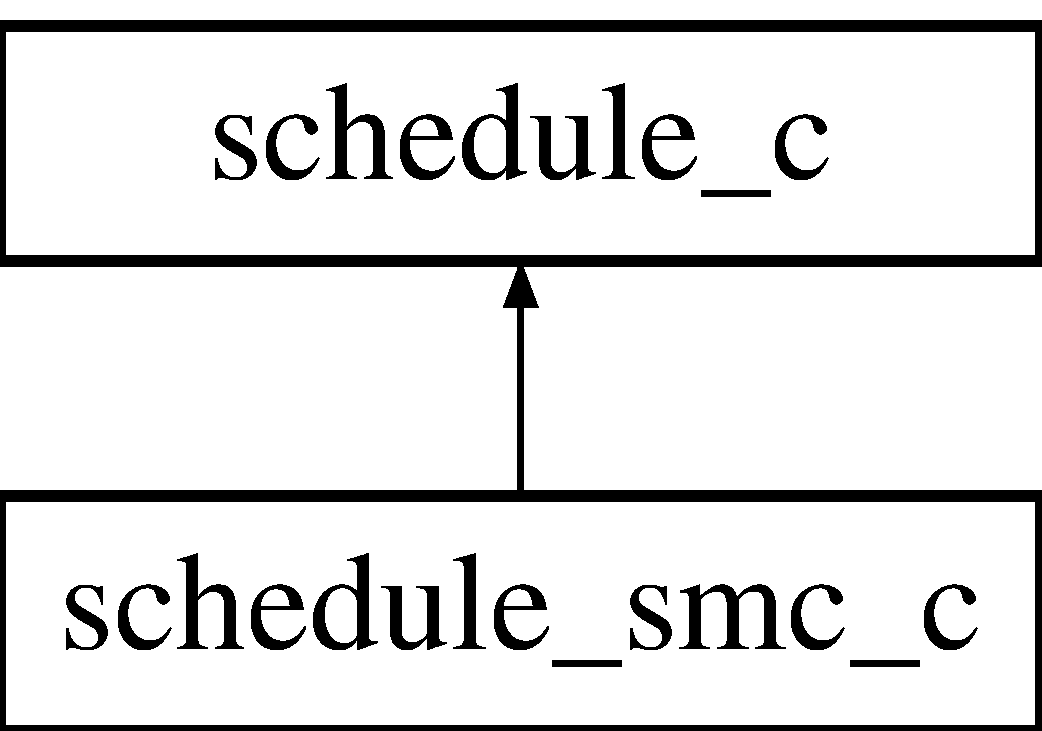
\includegraphics[height=2.000000cm]{classschedule__smc__c}
\end{center}
\end{figure}
\subsection*{Public Member Functions}
\begin{DoxyCompactItemize}
\item 
\hyperlink{classschedule__smc__c_ac95fdbfe0f924722b86e10deb736d7d9}{schedule\_\-smc\_\-c} (int \hyperlink{classschedule__c_a6c4f8484b3f2dae8255c0ce064f9d46e}{m\_\-core\_\-id}, \hyperlink{classpqueue__c}{pqueue\_\-c}$<$ \hyperlink{structgpu__allocq__entry__s}{gpu\_\-allocq\_\-entry\_\-s} $>$ $\ast$$\ast$gpu\_\-allocq, \hyperlink{classsmc__rob__c}{smc\_\-rob\_\-c} $\ast$gpu\_\-m\_\-rob, \hyperlink{classexec__c}{exec\_\-c} $\ast$\hyperlink{classschedule__c_a75e32c0fe0d1ad336ada30787fceafd8}{m\_\-exec}, Unit\_\-Type \hyperlink{classschedule__c_a5fd7913b69e838b56da18de2802d8a71}{m\_\-unit\_\-type}, \hyperlink{classfrontend__c}{frontend\_\-c} $\ast$\hyperlink{classschedule__c_a88ee09e9569c248374f0c943a4b73987}{m\_\-frontend}, \hyperlink{classmacsim__c}{macsim\_\-c} $\ast$simBase)
\begin{DoxyCompactList}\small\item\em Constructor for the gpu scheluder class. \item\end{DoxyCompactList}\item 
\hyperlink{classschedule__smc__c_aea8405348022655c30f22dfbe9447eda}{$\sim$schedule\_\-smc\_\-c} (void)
\begin{DoxyCompactList}\small\item\em Destructor for the gpu scheduler. \item\end{DoxyCompactList}\item 
void \hyperlink{classschedule__smc__c_aeb80c4988ef300b7dbd8f54fadc1a2ae}{run\_\-a\_\-cycle} ()
\begin{DoxyCompactList}\small\item\em Function to perform the activities of a cycle for the scheduler. \item\end{DoxyCompactList}\end{DoxyCompactItemize}
\subsection*{Private Member Functions}
\begin{DoxyCompactItemize}
\item 
void \hyperlink{classschedule__smc__c_a7f3ddbde213ee0afe9ba6af280bd6410}{advance} (int ALLOCQ\_\-index)
\begin{DoxyCompactList}\small\item\em Function to move the allocation queue ahead. \item\end{DoxyCompactList}\item 
bool \hyperlink{classschedule__smc__c_acb5620b01fbcee7106da60275f6c4ec1}{check\_\-srcs} (int thread\_\-id, int entry)
\begin{DoxyCompactList}\small\item\em Function to check if the sources of an uop are ready. \item\end{DoxyCompactList}\item 
bool \hyperlink{classschedule__smc__c_a663a2b4622b94a2b2b64110b5787015c}{uop\_\-schedule} (int thread\_\-id, int entry, SCHED\_\-FAIL\_\-TYPE $\ast$sched\_\-fail\_\-reason)
\begin{DoxyCompactList}\small\item\em Function to schedule uops. \item\end{DoxyCompactList}\end{DoxyCompactItemize}
\subsection*{Private Attributes}
\begin{DoxyCompactItemize}
\item 
\hyperlink{classsmc__rob__c}{smc\_\-rob\_\-c} $\ast$ \hyperlink{classschedule__smc__c_a9010fc8b51522f02c9742f7c9498805b}{m\_\-gpu\_\-rob}
\item 
\hyperlink{classpqueue__c}{pqueue\_\-c}$<$ \hyperlink{structgpu__allocq__entry__s}{gpu\_\-allocq\_\-entry\_\-s} $>$ $\ast$$\ast$ \hyperlink{classschedule__smc__c_a8862c810b1e0da537ef0a5b7b7e8e2b6}{m\_\-gpu\_\-allocq}
\item 
int \hyperlink{classschedule__smc__c_a615d15485be9b13e8f62ed984acc588e}{knob\_\-num\_\-threads}
\item 
int \hyperlink{classschedule__smc__c_aeb0d028cbba234e9e93abede46bba2ca}{m\_\-schedule\_\-modulo}
\item 
\hypertarget{classschedule__smc__c_a7a1cd319f4e01bc323443722b77fbc24}{
int $\ast$ {\bfseries m\_\-schlist\_\-entry}}
\label{classschedule__smc__c_a7a1cd319f4e01bc323443722b77fbc24}

\item 
\hypertarget{classschedule__smc__c_a33117e5fec2a6e9b62f028c04186bbf5}{
int $\ast$ {\bfseries m\_\-schlist\_\-tid}}
\label{classschedule__smc__c_a33117e5fec2a6e9b62f028c04186bbf5}

\item 
\hypertarget{classschedule__smc__c_aacd48030e596766416ed7ac22fcfb9fb}{
int {\bfseries m\_\-first\_\-schlist}}
\label{classschedule__smc__c_aacd48030e596766416ed7ac22fcfb9fb}

\item 
\hypertarget{classschedule__smc__c_a00ae6f68a0eec8a62ed44381329ee6b8}{
int {\bfseries m\_\-last\_\-schlist}}
\label{classschedule__smc__c_a00ae6f68a0eec8a62ed44381329ee6b8}

\item 
\hypertarget{classschedule__smc__c_a60aa9c8f3eea2e35f0298320fd4d0783}{
int {\bfseries m\_\-schlist\_\-size}}
\label{classschedule__smc__c_a60aa9c8f3eea2e35f0298320fd4d0783}

\item 
\hyperlink{classmacsim__c}{macsim\_\-c} $\ast$ \hyperlink{classschedule__smc__c_a40d5c66331f8f72123691ebbb4590f3b}{m\_\-simBase}
\end{DoxyCompactItemize}
\subsection*{Static Private Attributes}
\begin{DoxyCompactItemize}
\item 
static const int \hyperlink{classschedule__smc__c_a70bea811c0a494c3741fa64b319b0001}{MAX\_\-GPU\_\-SCHED\_\-SIZE} = 128
\end{DoxyCompactItemize}


\subsection{Detailed Description}
Scheduler class for GPU simulation. 

\subsection{Constructor \& Destructor Documentation}
\hypertarget{classschedule__smc__c_ac95fdbfe0f924722b86e10deb736d7d9}{
\index{schedule\_\-smc\_\-c@{schedule\_\-smc\_\-c}!schedule\_\-smc\_\-c@{schedule\_\-smc\_\-c}}
\index{schedule\_\-smc\_\-c@{schedule\_\-smc\_\-c}!schedule_smc_c@{schedule\_\-smc\_\-c}}
\subsubsection[{schedule\_\-smc\_\-c}]{\setlength{\rightskip}{0pt plus 5cm}schedule\_\-smc\_\-c::schedule\_\-smc\_\-c (
\begin{DoxyParamCaption}
\item[{int}]{ m\_\-core\_\-id, }
\item[{{\bf pqueue\_\-c}$<$ {\bf gpu\_\-allocq\_\-entry\_\-s} $>$ $\ast$$\ast$}]{ gpu\_\-allocq, }
\item[{{\bf smc\_\-rob\_\-c} $\ast$}]{ gpu\_\-m\_\-rob, }
\item[{{\bf exec\_\-c} $\ast$}]{ m\_\-exec, }
\item[{Unit\_\-Type}]{ m\_\-unit\_\-type, }
\item[{{\bf frontend\_\-c} $\ast$}]{ m\_\-frontend, }
\item[{{\bf macsim\_\-c} $\ast$}]{ simBase}
\end{DoxyParamCaption}
)}}
\label{classschedule__smc__c_ac95fdbfe0f924722b86e10deb736d7d9}


Constructor for the gpu scheluder class. 


\begin{DoxyParams}{Parameters}
\item[{\em m\_\-core\_\-id}]-\/ Core identifier number \item[{\em gpu\_\-allocq}]-\/ Pointer to be updated with the alloc stage queues \item[{\em gpu\_\-m\_\-rob}]-\/ Pointer to the Reorder buffer \item[{\em m\_\-exec}]-\/ Pointer to m\_\-execution unit \item[{\em m\_\-unit\_\-type}]-\/ Parameter used to identify knob width \item[{\em m\_\-frontend}]-\/ Pointer to front end queue \end{DoxyParams}
\begin{DoxyReturn}{Returns}
void 
\end{DoxyReturn}
\hypertarget{classschedule__smc__c_aea8405348022655c30f22dfbe9447eda}{
\index{schedule\_\-smc\_\-c@{schedule\_\-smc\_\-c}!$\sim$schedule\_\-smc\_\-c@{$\sim$schedule\_\-smc\_\-c}}
\index{$\sim$schedule\_\-smc\_\-c@{$\sim$schedule\_\-smc\_\-c}!schedule_smc_c@{schedule\_\-smc\_\-c}}
\subsubsection[{$\sim$schedule\_\-smc\_\-c}]{\setlength{\rightskip}{0pt plus 5cm}void schedule\_\-smc\_\-c::$\sim$schedule\_\-smc\_\-c (
\begin{DoxyParamCaption}
\item[{void}]{}
\end{DoxyParamCaption}
)}}
\label{classschedule__smc__c_aea8405348022655c30f22dfbe9447eda}


Destructor for the gpu scheduler. 

\begin{DoxyReturn}{Returns}
void 
\end{DoxyReturn}


\subsection{Member Function Documentation}
\hypertarget{classschedule__smc__c_a7f3ddbde213ee0afe9ba6af280bd6410}{
\index{schedule\_\-smc\_\-c@{schedule\_\-smc\_\-c}!advance@{advance}}
\index{advance@{advance}!schedule_smc_c@{schedule\_\-smc\_\-c}}
\subsubsection[{advance}]{\setlength{\rightskip}{0pt plus 5cm}void schedule\_\-smc\_\-c::advance (
\begin{DoxyParamCaption}
\item[{int}]{ ALLOCQ\_\-index}
\end{DoxyParamCaption}
)\hspace{0.3cm}{\ttfamily  \mbox{[}private, virtual\mbox{]}}}}
\label{classschedule__smc__c_a7f3ddbde213ee0afe9ba6af280bd6410}


Function to move the allocation queue ahead. 


\begin{DoxyParams}{Parameters}
\item[{\em ALLOCQ\_\-index}]-\/ Aloocation queue number to be moved ahead \end{DoxyParams}
\begin{DoxyReturn}{Returns}
void 
\end{DoxyReturn}


Reimplemented from \hyperlink{classschedule__c_a35f2f1ea49453967c863c5de1acae87e}{schedule\_\-c}.

\hypertarget{classschedule__smc__c_acb5620b01fbcee7106da60275f6c4ec1}{
\index{schedule\_\-smc\_\-c@{schedule\_\-smc\_\-c}!check\_\-srcs@{check\_\-srcs}}
\index{check\_\-srcs@{check\_\-srcs}!schedule_smc_c@{schedule\_\-smc\_\-c}}
\subsubsection[{check\_\-srcs}]{\setlength{\rightskip}{0pt plus 5cm}bool schedule\_\-smc\_\-c::check\_\-srcs (
\begin{DoxyParamCaption}
\item[{int}]{ thread\_\-id, }
\item[{int}]{ entry}
\end{DoxyParamCaption}
)\hspace{0.3cm}{\ttfamily  \mbox{[}private\mbox{]}}}}
\label{classschedule__smc__c_acb5620b01fbcee7106da60275f6c4ec1}


Function to check if the sources of an uop are ready. 


\begin{DoxyParams}{Parameters}
\item[{\em thread\_\-id}]-\/ Thread id \item[{\em entry}]-\/ ROB entry of the uop \end{DoxyParams}
\begin{DoxyReturn}{Returns}
bool -\/ True if no dependency found 
\end{DoxyReturn}
\hypertarget{classschedule__smc__c_aeb80c4988ef300b7dbd8f54fadc1a2ae}{
\index{schedule\_\-smc\_\-c@{schedule\_\-smc\_\-c}!run\_\-a\_\-cycle@{run\_\-a\_\-cycle}}
\index{run\_\-a\_\-cycle@{run\_\-a\_\-cycle}!schedule_smc_c@{schedule\_\-smc\_\-c}}
\subsubsection[{run\_\-a\_\-cycle}]{\setlength{\rightskip}{0pt plus 5cm}void schedule\_\-smc\_\-c::run\_\-a\_\-cycle (
\begin{DoxyParamCaption}
\item[{void}]{}
\end{DoxyParamCaption}
)\hspace{0.3cm}{\ttfamily  \mbox{[}virtual\mbox{]}}}}
\label{classschedule__smc__c_aeb80c4988ef300b7dbd8f54fadc1a2ae}


Function to perform the activities of a cycle for the scheduler. 

\begin{DoxyReturn}{Returns}
void 
\end{DoxyReturn}


Implements \hyperlink{classschedule__c_abaede0d6b5e70e5cfc6bf98801e387e1}{schedule\_\-c}.

\hypertarget{classschedule__smc__c_a663a2b4622b94a2b2b64110b5787015c}{
\index{schedule\_\-smc\_\-c@{schedule\_\-smc\_\-c}!uop\_\-schedule@{uop\_\-schedule}}
\index{uop\_\-schedule@{uop\_\-schedule}!schedule_smc_c@{schedule\_\-smc\_\-c}}
\subsubsection[{uop\_\-schedule}]{\setlength{\rightskip}{0pt plus 5cm}bool schedule\_\-smc\_\-c::uop\_\-schedule (
\begin{DoxyParamCaption}
\item[{int}]{ thread\_\-id, }
\item[{int}]{ entry, }
\item[{SCHED\_\-FAIL\_\-TYPE $\ast$}]{ sched\_\-fail\_\-reason}
\end{DoxyParamCaption}
)\hspace{0.3cm}{\ttfamily  \mbox{[}private\mbox{]}}}}
\label{classschedule__smc__c_a663a2b4622b94a2b2b64110b5787015c}


Function to schedule uops. 


\begin{DoxyParams}{Parameters}
\item[{\em thread\_\-id}]-\/ Thread id \item[{\em entry}]-\/ ROB entry of the uop \item[{\em sched\_\-fail\_\-reason}]-\/ Reason of uop schedule failure \end{DoxyParams}
\begin{DoxyReturn}{Returns}
bool -\/ True on success in scheduling 
\end{DoxyReturn}


\subsection{Member Data Documentation}
\hypertarget{classschedule__smc__c_a615d15485be9b13e8f62ed984acc588e}{
\index{schedule\_\-smc\_\-c@{schedule\_\-smc\_\-c}!knob\_\-num\_\-threads@{knob\_\-num\_\-threads}}
\index{knob\_\-num\_\-threads@{knob\_\-num\_\-threads}!schedule_smc_c@{schedule\_\-smc\_\-c}}
\subsubsection[{knob\_\-num\_\-threads}]{\setlength{\rightskip}{0pt plus 5cm}int {\bf schedule\_\-smc\_\-c::knob\_\-num\_\-threads}\hspace{0.3cm}{\ttfamily  \mbox{[}private\mbox{]}}}}
\label{classschedule__smc__c_a615d15485be9b13e8f62ed984acc588e}
number of maximum thread per core \hypertarget{classschedule__smc__c_a8862c810b1e0da537ef0a5b7b7e8e2b6}{
\index{schedule\_\-smc\_\-c@{schedule\_\-smc\_\-c}!m\_\-gpu\_\-allocq@{m\_\-gpu\_\-allocq}}
\index{m\_\-gpu\_\-allocq@{m\_\-gpu\_\-allocq}!schedule_smc_c@{schedule\_\-smc\_\-c}}
\subsubsection[{m\_\-gpu\_\-allocq}]{\setlength{\rightskip}{0pt plus 5cm}{\bf pqueue\_\-c}$<${\bf gpu\_\-allocq\_\-entry\_\-s}$>$$\ast$$\ast$ {\bf schedule\_\-smc\_\-c::m\_\-gpu\_\-allocq}\hspace{0.3cm}{\ttfamily  \mbox{[}private\mbox{]}}}}
\label{classschedule__smc__c_a8862c810b1e0da537ef0a5b7b7e8e2b6}
gpu allocation queue \hypertarget{classschedule__smc__c_a9010fc8b51522f02c9742f7c9498805b}{
\index{schedule\_\-smc\_\-c@{schedule\_\-smc\_\-c}!m\_\-gpu\_\-rob@{m\_\-gpu\_\-rob}}
\index{m\_\-gpu\_\-rob@{m\_\-gpu\_\-rob}!schedule_smc_c@{schedule\_\-smc\_\-c}}
\subsubsection[{m\_\-gpu\_\-rob}]{\setlength{\rightskip}{0pt plus 5cm}{\bf smc\_\-rob\_\-c}$\ast$ {\bf schedule\_\-smc\_\-c::m\_\-gpu\_\-rob}\hspace{0.3cm}{\ttfamily  \mbox{[}private\mbox{]}}}}
\label{classschedule__smc__c_a9010fc8b51522f02c9742f7c9498805b}
gpu rob \hypertarget{classschedule__smc__c_aeb0d028cbba234e9e93abede46bba2ca}{
\index{schedule\_\-smc\_\-c@{schedule\_\-smc\_\-c}!m\_\-schedule\_\-modulo@{m\_\-schedule\_\-modulo}}
\index{m\_\-schedule\_\-modulo@{m\_\-schedule\_\-modulo}!schedule_smc_c@{schedule\_\-smc\_\-c}}
\subsubsection[{m\_\-schedule\_\-modulo}]{\setlength{\rightskip}{0pt plus 5cm}int {\bf schedule\_\-smc\_\-c::m\_\-schedule\_\-modulo}\hspace{0.3cm}{\ttfamily  \mbox{[}private\mbox{]}}}}
\label{classschedule__smc__c_aeb0d028cbba234e9e93abede46bba2ca}
modulo to schedule next thread \hypertarget{classschedule__smc__c_a40d5c66331f8f72123691ebbb4590f3b}{
\index{schedule\_\-smc\_\-c@{schedule\_\-smc\_\-c}!m\_\-simBase@{m\_\-simBase}}
\index{m\_\-simBase@{m\_\-simBase}!schedule_smc_c@{schedule\_\-smc\_\-c}}
\subsubsection[{m\_\-simBase}]{\setlength{\rightskip}{0pt plus 5cm}{\bf macsim\_\-c}$\ast$ {\bf schedule\_\-smc\_\-c::m\_\-simBase}\hspace{0.3cm}{\ttfamily  \mbox{[}private\mbox{]}}}}
\label{classschedule__smc__c_a40d5c66331f8f72123691ebbb4590f3b}
\hyperlink{classmacsim__c}{macsim\_\-c} base class for simulation globals 

Reimplemented from \hyperlink{classschedule__c_a0db71234050b2c33f454b5d65d458564}{schedule\_\-c}.

\hypertarget{classschedule__smc__c_a70bea811c0a494c3741fa64b319b0001}{
\index{schedule\_\-smc\_\-c@{schedule\_\-smc\_\-c}!MAX\_\-GPU\_\-SCHED\_\-SIZE@{MAX\_\-GPU\_\-SCHED\_\-SIZE}}
\index{MAX\_\-GPU\_\-SCHED\_\-SIZE@{MAX\_\-GPU\_\-SCHED\_\-SIZE}!schedule_smc_c@{schedule\_\-smc\_\-c}}
\subsubsection[{MAX\_\-GPU\_\-SCHED\_\-SIZE}]{\setlength{\rightskip}{0pt plus 5cm}const int {\bf schedule\_\-smc\_\-c::MAX\_\-GPU\_\-SCHED\_\-SIZE} = 128\hspace{0.3cm}{\ttfamily  \mbox{[}static, private\mbox{]}}}}
\label{classschedule__smc__c_a70bea811c0a494c3741fa64b319b0001}
max sched table size 

The documentation for this class was generated from the following files:\begin{DoxyCompactItemize}
\item 
schedule\_\-smc.h\item 
schedule\_\-smc.cc\end{DoxyCompactItemize}

\hypertarget{structsection__info__s}{
\section{section\_\-info\_\-s Struct Reference}
\label{structsection__info__s}\index{section\_\-info\_\-s@{section\_\-info\_\-s}}
}


Section information.  




{\ttfamily \#include $<$process\_\-manager.h$>$}

\subsection*{Public Attributes}
\begin{DoxyCompactItemize}
\item 
Section\_\-Type\_\-enum \hyperlink{structsection__info__s_a8a3c90037442b973b1fbfd11893af7f8}{m\_\-section\_\-type}
\item 
int32\_\-t \hyperlink{structsection__info__s_a9338972d43c2662c79d169671a6c72b2}{m\_\-section\_\-length}
\end{DoxyCompactItemize}


\subsection{Detailed Description}
Section information. A section consists of few instruction. There are several types \begin{DoxySeeAlso}{See also}
Section\_\-Type\_\-enum 
\end{DoxySeeAlso}


\subsection{Member Data Documentation}
\hypertarget{structsection__info__s_a9338972d43c2662c79d169671a6c72b2}{
\index{section\_\-info\_\-s@{section\_\-info\_\-s}!m\_\-section\_\-length@{m\_\-section\_\-length}}
\index{m\_\-section\_\-length@{m\_\-section\_\-length}!section_info_s@{section\_\-info\_\-s}}
\subsubsection[{m\_\-section\_\-length}]{\setlength{\rightskip}{0pt plus 5cm}int32\_\-t {\bf section\_\-info\_\-s::m\_\-section\_\-length}}}
\label{structsection__info__s_a9338972d43c2662c79d169671a6c72b2}
section length in instruction counts \hypertarget{structsection__info__s_a8a3c90037442b973b1fbfd11893af7f8}{
\index{section\_\-info\_\-s@{section\_\-info\_\-s}!m\_\-section\_\-type@{m\_\-section\_\-type}}
\index{m\_\-section\_\-type@{m\_\-section\_\-type}!section_info_s@{section\_\-info\_\-s}}
\subsubsection[{m\_\-section\_\-type}]{\setlength{\rightskip}{0pt plus 5cm}Section\_\-Type\_\-enum {\bf section\_\-info\_\-s::m\_\-section\_\-type}}}
\label{structsection__info__s_a8a3c90037442b973b1fbfd11893af7f8}
section type 

The documentation for this struct was generated from the following file:\begin{DoxyCompactItemize}
\item 
process\_\-manager.h\end{DoxyCompactItemize}

\hypertarget{classsmc__allocate__c}{
\section{smc\_\-allocate\_\-c Class Reference}
\label{classsmc__allocate__c}\index{smc\_\-allocate\_\-c@{smc\_\-allocate\_\-c}}
}


Allocation stage for GPU simulation.  




{\ttfamily \#include $<$allocate\_\-smc.h$>$}

\subsection*{Public Member Functions}
\begin{DoxyCompactItemize}
\item 
\hyperlink{classsmc__allocate__c_afd008391634a752b54573173db52be11}{smc\_\-allocate\_\-c} (int core\_\-id, \hyperlink{classpqueue__c}{pqueue\_\-c}$<$ int $\ast$ $>$ $\ast$q\_\-frontend, \hyperlink{classpqueue__c}{pqueue\_\-c}$<$ \hyperlink{structgpu__allocq__entry__s}{gpu\_\-allocq\_\-entry\_\-s} $>$ $\ast$$\ast$gpu\_\-alloc\_\-q, \hyperlink{classpool__c}{pool\_\-c}$<$ \hyperlink{classuop__c}{uop\_\-c} $>$ $\ast$uop\_\-pool, \hyperlink{classsmc__rob__c}{smc\_\-rob\_\-c} $\ast$gpu\_\-rob, Unit\_\-Type unit\_\-type, int num\_\-queues, \hyperlink{classmacsim__c}{macsim\_\-c} $\ast$simBase)
\begin{DoxyCompactList}\small\item\em Create a data structures needed for the allocation stage in the pipeline. \item\end{DoxyCompactList}\item 
\hyperlink{classsmc__allocate__c_a58bf0515b7fe139787c1808f45a5f45a}{$\sim$smc\_\-allocate\_\-c} ()
\begin{DoxyCompactList}\small\item\em Destructor. \item\end{DoxyCompactList}\item 
void \hyperlink{classsmc__allocate__c_a127be98f456d4c2d30985e73e37cfd67}{run\_\-a\_\-cycle} ()
\item 
void \hyperlink{classsmc__allocate__c_a29566786181c9e5963324f2061d9982f}{start} ()
\begin{DoxyCompactList}\small\item\em Mark allocation as running. \item\end{DoxyCompactList}\item 
void \hyperlink{classsmc__allocate__c_acf8790fcc3c948f6d2cf887c3db81652}{stop} ()
\begin{DoxyCompactList}\small\item\em Mark allocation as halted. \item\end{DoxyCompactList}\item 
bool \hyperlink{classsmc__allocate__c_ab7431c27506fdfa1c58d39c9ae9e5472}{is\_\-running} ()
\begin{DoxyCompactList}\small\item\em Check if allocation stage is running i.e., not halted. \item\end{DoxyCompactList}\end{DoxyCompactItemize}
\subsection*{Private Attributes}
\begin{DoxyCompactItemize}
\item 
int \hyperlink{classsmc__allocate__c_abaeb422a48ef93fb71cabc5390dee7b9}{m\_\-core\_\-id}
\item 
\hyperlink{classpqueue__c}{pqueue\_\-c}$<$ int $\ast$ $>$ $\ast$ \hyperlink{classsmc__allocate__c_a3db2b8a63184bcda1bd1d9a2231becf7}{m\_\-frontend\_\-q}
\item 
\hyperlink{classpqueue__c}{pqueue\_\-c}$<$ \hyperlink{structgpu__allocq__entry__s}{gpu\_\-allocq\_\-entry\_\-s} $>$ $\ast$$\ast$ \hyperlink{classsmc__allocate__c_ad36b7e814f1f2199295dce4d617ff035}{m\_\-gpu\_\-alloc\_\-q}
\item 
\hyperlink{classpool__c}{pool\_\-c}$<$ \hyperlink{classuop__c}{uop\_\-c} $>$ $\ast$ \hyperlink{classsmc__allocate__c_a1fce12aa293716b7c3ea687c0400dcf3}{m\_\-uop\_\-pool}
\item 
\hyperlink{classsmc__rob__c}{smc\_\-rob\_\-c} $\ast$ \hyperlink{classsmc__allocate__c_a8975102c918ebb18ff50b054d70fd1a3}{m\_\-gpu\_\-rob}
\item 
Unit\_\-Type \hyperlink{classsmc__allocate__c_aeb14fe67ed777300d891a22ed3db120d}{m\_\-unit\_\-type}
\item 
uns16 \hyperlink{classsmc__allocate__c_a5cdf0163de169d08e9b51a760381c66d}{m\_\-knob\_\-width}
\item 
bool \hyperlink{classsmc__allocate__c_a8369b4404232451b5fec0eff0d6ef011}{m\_\-allocate\_\-running}
\item 
Counter \hyperlink{classsmc__allocate__c_ae5879c983f2dd0520f6fb4e76d90271f}{m\_\-cur\_\-core\_\-cycle}
\item 
int \hyperlink{classsmc__allocate__c_afea356100a59d2bf67ee102c1e41e4f2}{m\_\-num\_\-queues}
\item 
\hyperlink{classmacsim__c}{macsim\_\-c} $\ast$ \hyperlink{classsmc__allocate__c_abd96160a09d01811d1920c3330731107}{m\_\-simBase}
\end{DoxyCompactItemize}


\subsection{Detailed Description}
Allocation stage for GPU simulation. 

\subsection{Constructor \& Destructor Documentation}
\hypertarget{classsmc__allocate__c_afd008391634a752b54573173db52be11}{
\index{smc\_\-allocate\_\-c@{smc\_\-allocate\_\-c}!smc\_\-allocate\_\-c@{smc\_\-allocate\_\-c}}
\index{smc\_\-allocate\_\-c@{smc\_\-allocate\_\-c}!smc_allocate_c@{smc\_\-allocate\_\-c}}
\subsubsection[{smc\_\-allocate\_\-c}]{\setlength{\rightskip}{0pt plus 5cm}smc\_\-allocate\_\-c::smc\_\-allocate\_\-c (
\begin{DoxyParamCaption}
\item[{int}]{ core\_\-id, }
\item[{{\bf pqueue\_\-c}$<$ int $\ast$ $>$ $\ast$}]{ q\_\-frontend, }
\item[{{\bf pqueue\_\-c}$<$ {\bf gpu\_\-allocq\_\-entry\_\-s} $>$ $\ast$$\ast$}]{ gpu\_\-alloc\_\-q, }
\item[{{\bf pool\_\-c}$<$ {\bf uop\_\-c} $>$ $\ast$}]{ uop\_\-pool, }
\item[{{\bf smc\_\-rob\_\-c} $\ast$}]{ gpu\_\-rob, }
\item[{Unit\_\-Type}]{ unit\_\-type, }
\item[{int}]{ num\_\-queues, }
\item[{{\bf macsim\_\-c} $\ast$}]{ simBase}
\end{DoxyParamCaption}
)}}
\label{classsmc__allocate__c_afd008391634a752b54573173db52be11}


Create a data structures needed for the allocation stage in the pipeline. 


\begin{DoxyParams}{Parameters}
\item[{\em core\_\-id}]Core identifier number \item[{\em q\_\-frontend}]Pointer to front end queue \item[{\em gpu\_\-alloc\_\-q}]Pointer to be updated with the allocation stage queue \item[{\em uop\_\-pool}]Pointer to uop pool \item[{\em gpu\_\-rob}]Pointer to the Reorder buffer \item[{\em unit\_\-type}]Parameter used to identify knob width \item[{\em num\_\-queues}]number of allocation queues \item[{\em simBase}]-\/ Pointer to base simulation class for perf/stat counters \end{DoxyParams}
\begin{DoxyReturn}{Returns}
void 
\end{DoxyReturn}
\hypertarget{classsmc__allocate__c_a58bf0515b7fe139787c1808f45a5f45a}{
\index{smc\_\-allocate\_\-c@{smc\_\-allocate\_\-c}!$\sim$smc\_\-allocate\_\-c@{$\sim$smc\_\-allocate\_\-c}}
\index{$\sim$smc\_\-allocate\_\-c@{$\sim$smc\_\-allocate\_\-c}!smc_allocate_c@{smc\_\-allocate\_\-c}}
\subsubsection[{$\sim$smc\_\-allocate\_\-c}]{\setlength{\rightskip}{0pt plus 5cm}smc\_\-allocate\_\-c::$\sim$smc\_\-allocate\_\-c (
\begin{DoxyParamCaption}
{}
\end{DoxyParamCaption}
)}}
\label{classsmc__allocate__c_a58bf0515b7fe139787c1808f45a5f45a}


Destructor. 

\begin{DoxyReturn}{Returns}
void 
\end{DoxyReturn}


\subsection{Member Function Documentation}
\hypertarget{classsmc__allocate__c_ab7431c27506fdfa1c58d39c9ae9e5472}{
\index{smc\_\-allocate\_\-c@{smc\_\-allocate\_\-c}!is\_\-running@{is\_\-running}}
\index{is\_\-running@{is\_\-running}!smc_allocate_c@{smc\_\-allocate\_\-c}}
\subsubsection[{is\_\-running}]{\setlength{\rightskip}{0pt plus 5cm}smc\_\-allocate\_\-c::is\_\-running (
\begin{DoxyParamCaption}
{}
\end{DoxyParamCaption}
)\hspace{0.3cm}{\ttfamily  \mbox{[}inline\mbox{]}}}}
\label{classsmc__allocate__c_ab7431c27506fdfa1c58d39c9ae9e5472}


Check if allocation stage is running i.e., not halted. 

\begin{DoxyReturn}{Returns}
void 
\end{DoxyReturn}
\hypertarget{classsmc__allocate__c_a127be98f456d4c2d30985e73e37cfd67}{
\index{smc\_\-allocate\_\-c@{smc\_\-allocate\_\-c}!run\_\-a\_\-cycle@{run\_\-a\_\-cycle}}
\index{run\_\-a\_\-cycle@{run\_\-a\_\-cycle}!smc_allocate_c@{smc\_\-allocate\_\-c}}
\subsubsection[{run\_\-a\_\-cycle}]{\setlength{\rightskip}{0pt plus 5cm}void smc\_\-allocate\_\-c::run\_\-a\_\-cycle (
\begin{DoxyParamCaption}
\item[{void}]{}
\end{DoxyParamCaption}
)}}
\label{classsmc__allocate__c_a127be98f456d4c2d30985e73e37cfd67}
Function to be called at each cycle by the simulator to perform the duties of the allocation stage. \hypertarget{classsmc__allocate__c_a29566786181c9e5963324f2061d9982f}{
\index{smc\_\-allocate\_\-c@{smc\_\-allocate\_\-c}!start@{start}}
\index{start@{start}!smc_allocate_c@{smc\_\-allocate\_\-c}}
\subsubsection[{start}]{\setlength{\rightskip}{0pt plus 5cm}smc\_\-allocate\_\-c::start (
\begin{DoxyParamCaption}
{}
\end{DoxyParamCaption}
)\hspace{0.3cm}{\ttfamily  \mbox{[}inline\mbox{]}}}}
\label{classsmc__allocate__c_a29566786181c9e5963324f2061d9982f}


Mark allocation as running. 

\begin{DoxyReturn}{Returns}
void 
\end{DoxyReturn}
\hypertarget{classsmc__allocate__c_acf8790fcc3c948f6d2cf887c3db81652}{
\index{smc\_\-allocate\_\-c@{smc\_\-allocate\_\-c}!stop@{stop}}
\index{stop@{stop}!smc_allocate_c@{smc\_\-allocate\_\-c}}
\subsubsection[{stop}]{\setlength{\rightskip}{0pt plus 5cm}smc\_\-allocate\_\-c::stop (
\begin{DoxyParamCaption}
{}
\end{DoxyParamCaption}
)\hspace{0.3cm}{\ttfamily  \mbox{[}inline\mbox{]}}}}
\label{classsmc__allocate__c_acf8790fcc3c948f6d2cf887c3db81652}


Mark allocation as halted. 

\begin{DoxyReturn}{Returns}
void 
\end{DoxyReturn}


\subsection{Member Data Documentation}
\hypertarget{classsmc__allocate__c_a8369b4404232451b5fec0eff0d6ef011}{
\index{smc\_\-allocate\_\-c@{smc\_\-allocate\_\-c}!m\_\-allocate\_\-running@{m\_\-allocate\_\-running}}
\index{m\_\-allocate\_\-running@{m\_\-allocate\_\-running}!smc_allocate_c@{smc\_\-allocate\_\-c}}
\subsubsection[{m\_\-allocate\_\-running}]{\setlength{\rightskip}{0pt plus 5cm}bool {\bf smc\_\-allocate\_\-c::m\_\-allocate\_\-running}\hspace{0.3cm}{\ttfamily  \mbox{[}private\mbox{]}}}}
\label{classsmc__allocate__c_a8369b4404232451b5fec0eff0d6ef011}
Enable allocation stage \hypertarget{classsmc__allocate__c_abaeb422a48ef93fb71cabc5390dee7b9}{
\index{smc\_\-allocate\_\-c@{smc\_\-allocate\_\-c}!m\_\-core\_\-id@{m\_\-core\_\-id}}
\index{m\_\-core\_\-id@{m\_\-core\_\-id}!smc_allocate_c@{smc\_\-allocate\_\-c}}
\subsubsection[{m\_\-core\_\-id}]{\setlength{\rightskip}{0pt plus 5cm}int {\bf smc\_\-allocate\_\-c::m\_\-core\_\-id}\hspace{0.3cm}{\ttfamily  \mbox{[}private\mbox{]}}}}
\label{classsmc__allocate__c_abaeb422a48ef93fb71cabc5390dee7b9}
core id \hypertarget{classsmc__allocate__c_ae5879c983f2dd0520f6fb4e76d90271f}{
\index{smc\_\-allocate\_\-c@{smc\_\-allocate\_\-c}!m\_\-cur\_\-core\_\-cycle@{m\_\-cur\_\-core\_\-cycle}}
\index{m\_\-cur\_\-core\_\-cycle@{m\_\-cur\_\-core\_\-cycle}!smc_allocate_c@{smc\_\-allocate\_\-c}}
\subsubsection[{m\_\-cur\_\-core\_\-cycle}]{\setlength{\rightskip}{0pt plus 5cm}Counter {\bf smc\_\-allocate\_\-c::m\_\-cur\_\-core\_\-cycle}\hspace{0.3cm}{\ttfamily  \mbox{[}private\mbox{]}}}}
\label{classsmc__allocate__c_ae5879c983f2dd0520f6fb4e76d90271f}
current core cycle \hypertarget{classsmc__allocate__c_a3db2b8a63184bcda1bd1d9a2231becf7}{
\index{smc\_\-allocate\_\-c@{smc\_\-allocate\_\-c}!m\_\-frontend\_\-q@{m\_\-frontend\_\-q}}
\index{m\_\-frontend\_\-q@{m\_\-frontend\_\-q}!smc_allocate_c@{smc\_\-allocate\_\-c}}
\subsubsection[{m\_\-frontend\_\-q}]{\setlength{\rightskip}{0pt plus 5cm}{\bf pqueue\_\-c}$<$int$\ast$$>$$\ast$ {\bf smc\_\-allocate\_\-c::m\_\-frontend\_\-q}\hspace{0.3cm}{\ttfamily  \mbox{[}private\mbox{]}}}}
\label{classsmc__allocate__c_a3db2b8a63184bcda1bd1d9a2231becf7}
frontend queue \hypertarget{classsmc__allocate__c_ad36b7e814f1f2199295dce4d617ff035}{
\index{smc\_\-allocate\_\-c@{smc\_\-allocate\_\-c}!m\_\-gpu\_\-alloc\_\-q@{m\_\-gpu\_\-alloc\_\-q}}
\index{m\_\-gpu\_\-alloc\_\-q@{m\_\-gpu\_\-alloc\_\-q}!smc_allocate_c@{smc\_\-allocate\_\-c}}
\subsubsection[{m\_\-gpu\_\-alloc\_\-q}]{\setlength{\rightskip}{0pt plus 5cm}{\bf pqueue\_\-c}$<${\bf gpu\_\-allocq\_\-entry\_\-s}$>$$\ast$$\ast$ {\bf smc\_\-allocate\_\-c::m\_\-gpu\_\-alloc\_\-q}\hspace{0.3cm}{\ttfamily  \mbox{[}private\mbox{]}}}}
\label{classsmc__allocate__c_ad36b7e814f1f2199295dce4d617ff035}
GPU allocation queue \hypertarget{classsmc__allocate__c_a8975102c918ebb18ff50b054d70fd1a3}{
\index{smc\_\-allocate\_\-c@{smc\_\-allocate\_\-c}!m\_\-gpu\_\-rob@{m\_\-gpu\_\-rob}}
\index{m\_\-gpu\_\-rob@{m\_\-gpu\_\-rob}!smc_allocate_c@{smc\_\-allocate\_\-c}}
\subsubsection[{m\_\-gpu\_\-rob}]{\setlength{\rightskip}{0pt plus 5cm}{\bf smc\_\-rob\_\-c}$\ast$ {\bf smc\_\-allocate\_\-c::m\_\-gpu\_\-rob}\hspace{0.3cm}{\ttfamily  \mbox{[}private\mbox{]}}}}
\label{classsmc__allocate__c_a8975102c918ebb18ff50b054d70fd1a3}
GPU reorder buffer \hypertarget{classsmc__allocate__c_a5cdf0163de169d08e9b51a760381c66d}{
\index{smc\_\-allocate\_\-c@{smc\_\-allocate\_\-c}!m\_\-knob\_\-width@{m\_\-knob\_\-width}}
\index{m\_\-knob\_\-width@{m\_\-knob\_\-width}!smc_allocate_c@{smc\_\-allocate\_\-c}}
\subsubsection[{m\_\-knob\_\-width}]{\setlength{\rightskip}{0pt plus 5cm}uns16 {\bf smc\_\-allocate\_\-c::m\_\-knob\_\-width}\hspace{0.3cm}{\ttfamily  \mbox{[}private\mbox{]}}}}
\label{classsmc__allocate__c_a5cdf0163de169d08e9b51a760381c66d}
width \hypertarget{classsmc__allocate__c_afea356100a59d2bf67ee102c1e41e4f2}{
\index{smc\_\-allocate\_\-c@{smc\_\-allocate\_\-c}!m\_\-num\_\-queues@{m\_\-num\_\-queues}}
\index{m\_\-num\_\-queues@{m\_\-num\_\-queues}!smc_allocate_c@{smc\_\-allocate\_\-c}}
\subsubsection[{m\_\-num\_\-queues}]{\setlength{\rightskip}{0pt plus 5cm}int {\bf smc\_\-allocate\_\-c::m\_\-num\_\-queues}\hspace{0.3cm}{\ttfamily  \mbox{[}private\mbox{]}}}}
\label{classsmc__allocate__c_afea356100a59d2bf67ee102c1e41e4f2}
number of allocation queue types \hypertarget{classsmc__allocate__c_abd96160a09d01811d1920c3330731107}{
\index{smc\_\-allocate\_\-c@{smc\_\-allocate\_\-c}!m\_\-simBase@{m\_\-simBase}}
\index{m\_\-simBase@{m\_\-simBase}!smc_allocate_c@{smc\_\-allocate\_\-c}}
\subsubsection[{m\_\-simBase}]{\setlength{\rightskip}{0pt plus 5cm}{\bf macsim\_\-c}$\ast$ {\bf smc\_\-allocate\_\-c::m\_\-simBase}\hspace{0.3cm}{\ttfamily  \mbox{[}private\mbox{]}}}}
\label{classsmc__allocate__c_abd96160a09d01811d1920c3330731107}
\hyperlink{classmacsim__c}{macsim\_\-c} base class for simulation globals \hypertarget{classsmc__allocate__c_aeb14fe67ed777300d891a22ed3db120d}{
\index{smc\_\-allocate\_\-c@{smc\_\-allocate\_\-c}!m\_\-unit\_\-type@{m\_\-unit\_\-type}}
\index{m\_\-unit\_\-type@{m\_\-unit\_\-type}!smc_allocate_c@{smc\_\-allocate\_\-c}}
\subsubsection[{m\_\-unit\_\-type}]{\setlength{\rightskip}{0pt plus 5cm}Unit\_\-Type {\bf smc\_\-allocate\_\-c::m\_\-unit\_\-type}\hspace{0.3cm}{\ttfamily  \mbox{[}private\mbox{]}}}}
\label{classsmc__allocate__c_aeb14fe67ed777300d891a22ed3db120d}
core type \hypertarget{classsmc__allocate__c_a1fce12aa293716b7c3ea687c0400dcf3}{
\index{smc\_\-allocate\_\-c@{smc\_\-allocate\_\-c}!m\_\-uop\_\-pool@{m\_\-uop\_\-pool}}
\index{m\_\-uop\_\-pool@{m\_\-uop\_\-pool}!smc_allocate_c@{smc\_\-allocate\_\-c}}
\subsubsection[{m\_\-uop\_\-pool}]{\setlength{\rightskip}{0pt plus 5cm}{\bf pool\_\-c}$<${\bf uop\_\-c}$>$$\ast$ {\bf smc\_\-allocate\_\-c::m\_\-uop\_\-pool}\hspace{0.3cm}{\ttfamily  \mbox{[}private\mbox{]}}}}
\label{classsmc__allocate__c_a1fce12aa293716b7c3ea687c0400dcf3}
uop pool 

The documentation for this class was generated from the following files:\begin{DoxyCompactItemize}
\item 
allocate\_\-smc.h\item 
allocate\_\-smc.cc\end{DoxyCompactItemize}

\hypertarget{classsmc__rob__c}{
\section{smc\_\-rob\_\-c Class Reference}
\label{classsmc__rob__c}\index{smc\_\-rob\_\-c@{smc\_\-rob\_\-c}}
}


Reorder buffer class for GPU simulation.  




{\ttfamily \#include $<$rob\_\-smc.h$>$}

\subsection*{Public Member Functions}
\begin{DoxyCompactItemize}
\item 
\hyperlink{classsmc__rob__c_a3491baac52db612930e0932193fb061b}{smc\_\-rob\_\-c} (Unit\_\-Type type, int core\_\-id, \hyperlink{classmacsim__c}{macsim\_\-c} $\ast$simBase)
\begin{DoxyCompactList}\small\item\em Create a Reorder Buffer data structure. \item\end{DoxyCompactList}\item 
\hyperlink{classsmc__rob__c_a423a152e2dbf5b69a199832581f492e5}{$\sim$smc\_\-rob\_\-c} ()
\begin{DoxyCompactList}\small\item\em Destructor. \item\end{DoxyCompactList}\item 
\hyperlink{classrob__c}{rob\_\-c} $\ast$ \hyperlink{classsmc__rob__c_afe3b3b1d744c1b9571c6fcdb0b844b93}{get\_\-thread\_\-rob} (int thread\_\-id)
\begin{DoxyCompactList}\small\item\em Function to return the corresponding ROB for the thread id. \item\end{DoxyCompactList}\item 
int \hyperlink{classsmc__rob__c_a53cf88f8da3879fe5f519d31d360a96e}{get\_\-thread\_\-rob\_\-id} (int thread\_\-id)
\begin{DoxyCompactList}\small\item\em Function to return the corresponding ROB index for the thread id. \item\end{DoxyCompactList}\item 
int \hyperlink{classsmc__rob__c_a48f8f093a1af607e9c3860804d4fd3f7}{reserve\_\-rob} (int thread\_\-id)
\begin{DoxyCompactList}\small\item\em Function to return the index of the ROB reserved. \item\end{DoxyCompactList}\item 
void \hyperlink{classsmc__rob__c_a16f7c053a3b618b6128ce079ea9636f0}{free\_\-rob} (int thread\_\-id)
\begin{DoxyCompactList}\small\item\em Function to free the ROB entry for the thread passed as parameter. \item\end{DoxyCompactList}\item 
vector$<$ \hyperlink{classuop__c}{uop\_\-c} $\ast$ $>$ $\ast$ \hyperlink{classsmc__rob__c_af76140ffac1f9cbb9de32f7e50618d14}{get\_\-n\_\-uops\_\-in\_\-ready\_\-order} (int n, Counter cur\_\-core\_\-cycle)
\begin{DoxyCompactList}\small\item\em Function to find the n most deserving uops to be retired. \item\end{DoxyCompactList}\end{DoxyCompactItemize}
\subsection*{Private Attributes}
\begin{DoxyCompactItemize}
\item 
int \hyperlink{classsmc__rob__c_a3fe15387db97e2865368976780a54db3}{m\_\-knob\_\-num\_\-threads}
\item 
\hyperlink{classrob__c}{rob\_\-c} $\ast$$\ast$ \hyperlink{classsmc__rob__c_a158a1f5f7421d05352318865b37e92bc}{m\_\-thread\_\-robs}
\item 
list$<$ int $>$ \hyperlink{classsmc__rob__c_a9db8c324e0133f306a0401ad53a52997}{m\_\-free\_\-list}
\item 
vector$<$ \hyperlink{classuop__c}{uop\_\-c} $\ast$ $>$ \hyperlink{classsmc__rob__c_a27d28e046bd5d8fbc76fefb6ad406423}{m\_\-uop\_\-list}
\item 
int \hyperlink{classsmc__rob__c_aad4bb4dd7c9e789a7f5d4d035f072649}{m\_\-core\_\-id}
\item 
Unit\_\-Type \hyperlink{classsmc__rob__c_a5b6e2bf88b64d1f769654120cd9d1f36}{m\_\-unit\_\-type}
\item 
unordered\_\-map$<$ int, int $>$ \hyperlink{classsmc__rob__c_a56ba9b44e042ed8f7cb752c1780ddf2e}{m\_\-thread\_\-to\_\-rob\_\-map}
\item 
\hyperlink{classmacsim__c}{macsim\_\-c} $\ast$ \hyperlink{classsmc__rob__c_a8f735f49a88a96ae31045a882dff660d}{m\_\-simBase}
\end{DoxyCompactItemize}


\subsection{Detailed Description}
Reorder buffer class for GPU simulation. 

\subsection{Constructor \& Destructor Documentation}
\hypertarget{classsmc__rob__c_a3491baac52db612930e0932193fb061b}{
\index{smc\_\-rob\_\-c@{smc\_\-rob\_\-c}!smc\_\-rob\_\-c@{smc\_\-rob\_\-c}}
\index{smc\_\-rob\_\-c@{smc\_\-rob\_\-c}!smc_rob_c@{smc\_\-rob\_\-c}}
\subsubsection[{smc\_\-rob\_\-c}]{\setlength{\rightskip}{0pt plus 5cm}smc\_\-rob\_\-c::smc\_\-rob\_\-c (
\begin{DoxyParamCaption}
\item[{Unit\_\-Type}]{ type, }
\item[{int}]{ core\_\-id, }
\item[{{\bf macsim\_\-c} $\ast$}]{ simBase}
\end{DoxyParamCaption}
)}}
\label{classsmc__rob__c_a3491baac52db612930e0932193fb061b}


Create a Reorder Buffer data structure. 


\begin{DoxyParams}{Parameters}
\item[{\em type}]-\/ Core type indicator \item[{\em core\_\-id}]-\/ core id \end{DoxyParams}
\begin{DoxyReturn}{Returns}
void. 
\end{DoxyReturn}
\hypertarget{classsmc__rob__c_a423a152e2dbf5b69a199832581f492e5}{
\index{smc\_\-rob\_\-c@{smc\_\-rob\_\-c}!$\sim$smc\_\-rob\_\-c@{$\sim$smc\_\-rob\_\-c}}
\index{$\sim$smc\_\-rob\_\-c@{$\sim$smc\_\-rob\_\-c}!smc_rob_c@{smc\_\-rob\_\-c}}
\subsubsection[{$\sim$smc\_\-rob\_\-c}]{\setlength{\rightskip}{0pt plus 5cm}void smc\_\-rob\_\-c::$\sim$smc\_\-rob\_\-c (
\begin{DoxyParamCaption}
{}
\end{DoxyParamCaption}
)}}
\label{classsmc__rob__c_a423a152e2dbf5b69a199832581f492e5}


Destructor. 

\begin{DoxyReturn}{Returns}
void. 
\end{DoxyReturn}


\subsection{Member Function Documentation}
\hypertarget{classsmc__rob__c_a16f7c053a3b618b6128ce079ea9636f0}{
\index{smc\_\-rob\_\-c@{smc\_\-rob\_\-c}!free\_\-rob@{free\_\-rob}}
\index{free\_\-rob@{free\_\-rob}!smc_rob_c@{smc\_\-rob\_\-c}}
\subsubsection[{free\_\-rob}]{\setlength{\rightskip}{0pt plus 5cm}void smc\_\-rob\_\-c::free\_\-rob (
\begin{DoxyParamCaption}
\item[{int}]{ thread\_\-id}
\end{DoxyParamCaption}
)}}
\label{classsmc__rob__c_a16f7c053a3b618b6128ce079ea9636f0}


Function to free the ROB entry for the thread passed as parameter. 


\begin{DoxyParams}{Parameters}
\item[{\em thread\_\-id}]Thread identifier \end{DoxyParams}
\begin{DoxyReturn}{Returns}
void. 
\end{DoxyReturn}
\hypertarget{classsmc__rob__c_af76140ffac1f9cbb9de32f7e50618d14}{
\index{smc\_\-rob\_\-c@{smc\_\-rob\_\-c}!get\_\-n\_\-uops\_\-in\_\-ready\_\-order@{get\_\-n\_\-uops\_\-in\_\-ready\_\-order}}
\index{get\_\-n\_\-uops\_\-in\_\-ready\_\-order@{get\_\-n\_\-uops\_\-in\_\-ready\_\-order}!smc_rob_c@{smc\_\-rob\_\-c}}
\subsubsection[{get\_\-n\_\-uops\_\-in\_\-ready\_\-order}]{\setlength{\rightskip}{0pt plus 5cm}list$<$ {\bf uop\_\-c} $\ast$ $>$ $\ast$ smc\_\-rob\_\-c::get\_\-n\_\-uops\_\-in\_\-ready\_\-order (
\begin{DoxyParamCaption}
\item[{int}]{ n, }
\item[{Counter}]{ cur\_\-core\_\-cycle}
\end{DoxyParamCaption}
)}}
\label{classsmc__rob__c_af76140ffac1f9cbb9de32f7e50618d14}


Function to find the n most deserving uops to be retired. 


\begin{DoxyParams}{Parameters}
\item[{\em n}]Count of Uopsmc\_\-rob.htrace \item[{\em cur\_\-core\_\-cycle}]Current core cycle \end{DoxyParams}
\begin{DoxyReturn}{Returns}
std::list$<$uop\_\-c $\ast$$>$$\ast$ . 
\end{DoxyReturn}
\hypertarget{classsmc__rob__c_afe3b3b1d744c1b9571c6fcdb0b844b93}{
\index{smc\_\-rob\_\-c@{smc\_\-rob\_\-c}!get\_\-thread\_\-rob@{get\_\-thread\_\-rob}}
\index{get\_\-thread\_\-rob@{get\_\-thread\_\-rob}!smc_rob_c@{smc\_\-rob\_\-c}}
\subsubsection[{get\_\-thread\_\-rob}]{\setlength{\rightskip}{0pt plus 5cm}void smc\_\-rob\_\-c::get\_\-thread\_\-rob (
\begin{DoxyParamCaption}
\item[{int}]{ thread\_\-id}
\end{DoxyParamCaption}
)}}
\label{classsmc__rob__c_afe3b3b1d744c1b9571c6fcdb0b844b93}


Function to return the corresponding ROB for the thread id. 


\begin{DoxyParams}{Parameters}
\item[{\em thread\_\-id}]Thread identifier \end{DoxyParams}
\begin{DoxyReturn}{Returns}
rob\_\-c$\ast$ ROB pointer. 
\end{DoxyReturn}
\hypertarget{classsmc__rob__c_a53cf88f8da3879fe5f519d31d360a96e}{
\index{smc\_\-rob\_\-c@{smc\_\-rob\_\-c}!get\_\-thread\_\-rob\_\-id@{get\_\-thread\_\-rob\_\-id}}
\index{get\_\-thread\_\-rob\_\-id@{get\_\-thread\_\-rob\_\-id}!smc_rob_c@{smc\_\-rob\_\-c}}
\subsubsection[{get\_\-thread\_\-rob\_\-id}]{\setlength{\rightskip}{0pt plus 5cm}int smc\_\-rob\_\-c::get\_\-thread\_\-rob\_\-id (
\begin{DoxyParamCaption}
\item[{int}]{ thread\_\-id}
\end{DoxyParamCaption}
)}}
\label{classsmc__rob__c_a53cf88f8da3879fe5f519d31d360a96e}


Function to return the corresponding ROB index for the thread id. 


\begin{DoxyParams}{Parameters}
\item[{\em thread\_\-id}]Thread identifier \end{DoxyParams}
\begin{DoxyReturn}{Returns}
int ROB index. 
\end{DoxyReturn}
\hypertarget{classsmc__rob__c_a48f8f093a1af607e9c3860804d4fd3f7}{
\index{smc\_\-rob\_\-c@{smc\_\-rob\_\-c}!reserve\_\-rob@{reserve\_\-rob}}
\index{reserve\_\-rob@{reserve\_\-rob}!smc_rob_c@{smc\_\-rob\_\-c}}
\subsubsection[{reserve\_\-rob}]{\setlength{\rightskip}{0pt plus 5cm}void int smc\_\-rob\_\-c::reserve\_\-rob (
\begin{DoxyParamCaption}
\item[{int}]{ thread\_\-id}
\end{DoxyParamCaption}
)}}
\label{classsmc__rob__c_a48f8f093a1af607e9c3860804d4fd3f7}


Function to return the index of the ROB reserved. 


\begin{DoxyParams}{Parameters}
\item[{\em thread\_\-id}]Thread identifier \end{DoxyParams}
\begin{DoxyReturn}{Returns}
int ROB index. 
\end{DoxyReturn}


\subsection{Member Data Documentation}
\hypertarget{classsmc__rob__c_aad4bb4dd7c9e789a7f5d4d035f072649}{
\index{smc\_\-rob\_\-c@{smc\_\-rob\_\-c}!m\_\-core\_\-id@{m\_\-core\_\-id}}
\index{m\_\-core\_\-id@{m\_\-core\_\-id}!smc_rob_c@{smc\_\-rob\_\-c}}
\subsubsection[{m\_\-core\_\-id}]{\setlength{\rightskip}{0pt plus 5cm}int {\bf smc\_\-rob\_\-c::m\_\-core\_\-id}\hspace{0.3cm}{\ttfamily  \mbox{[}private\mbox{]}}}}
\label{classsmc__rob__c_aad4bb4dd7c9e789a7f5d4d035f072649}
core id \hypertarget{classsmc__rob__c_a9db8c324e0133f306a0401ad53a52997}{
\index{smc\_\-rob\_\-c@{smc\_\-rob\_\-c}!m\_\-free\_\-list@{m\_\-free\_\-list}}
\index{m\_\-free\_\-list@{m\_\-free\_\-list}!smc_rob_c@{smc\_\-rob\_\-c}}
\subsubsection[{m\_\-free\_\-list}]{\setlength{\rightskip}{0pt plus 5cm}list$<$int$>$ {\bf smc\_\-rob\_\-c::m\_\-free\_\-list}\hspace{0.3cm}{\ttfamily  \mbox{[}private\mbox{]}}}}
\label{classsmc__rob__c_a9db8c324e0133f306a0401ad53a52997}
thread rob pool \hypertarget{classsmc__rob__c_a3fe15387db97e2865368976780a54db3}{
\index{smc\_\-rob\_\-c@{smc\_\-rob\_\-c}!m\_\-knob\_\-num\_\-threads@{m\_\-knob\_\-num\_\-threads}}
\index{m\_\-knob\_\-num\_\-threads@{m\_\-knob\_\-num\_\-threads}!smc_rob_c@{smc\_\-rob\_\-c}}
\subsubsection[{m\_\-knob\_\-num\_\-threads}]{\setlength{\rightskip}{0pt plus 5cm}int {\bf smc\_\-rob\_\-c::m\_\-knob\_\-num\_\-threads}\hspace{0.3cm}{\ttfamily  \mbox{[}private\mbox{]}}}}
\label{classsmc__rob__c_a3fe15387db97e2865368976780a54db3}
max threads per core \hypertarget{classsmc__rob__c_a8f735f49a88a96ae31045a882dff660d}{
\index{smc\_\-rob\_\-c@{smc\_\-rob\_\-c}!m\_\-simBase@{m\_\-simBase}}
\index{m\_\-simBase@{m\_\-simBase}!smc_rob_c@{smc\_\-rob\_\-c}}
\subsubsection[{m\_\-simBase}]{\setlength{\rightskip}{0pt plus 5cm}{\bf macsim\_\-c}$\ast$ {\bf smc\_\-rob\_\-c::m\_\-simBase}\hspace{0.3cm}{\ttfamily  \mbox{[}private\mbox{]}}}}
\label{classsmc__rob__c_a8f735f49a88a96ae31045a882dff660d}
\hyperlink{classmacsim__c}{macsim\_\-c} base class for simulation globals \hypertarget{classsmc__rob__c_a158a1f5f7421d05352318865b37e92bc}{
\index{smc\_\-rob\_\-c@{smc\_\-rob\_\-c}!m\_\-thread\_\-robs@{m\_\-thread\_\-robs}}
\index{m\_\-thread\_\-robs@{m\_\-thread\_\-robs}!smc_rob_c@{smc\_\-rob\_\-c}}
\subsubsection[{m\_\-thread\_\-robs}]{\setlength{\rightskip}{0pt plus 5cm}{\bf rob\_\-c}$\ast$$\ast$ {\bf smc\_\-rob\_\-c::m\_\-thread\_\-robs}\hspace{0.3cm}{\ttfamily  \mbox{[}private\mbox{]}}}}
\label{classsmc__rob__c_a158a1f5f7421d05352318865b37e92bc}
reorder buffer per thread \hypertarget{classsmc__rob__c_a56ba9b44e042ed8f7cb752c1780ddf2e}{
\index{smc\_\-rob\_\-c@{smc\_\-rob\_\-c}!m\_\-thread\_\-to\_\-rob\_\-map@{m\_\-thread\_\-to\_\-rob\_\-map}}
\index{m\_\-thread\_\-to\_\-rob\_\-map@{m\_\-thread\_\-to\_\-rob\_\-map}!smc_rob_c@{smc\_\-rob\_\-c}}
\subsubsection[{m\_\-thread\_\-to\_\-rob\_\-map}]{\setlength{\rightskip}{0pt plus 5cm}unordered\_\-map$<$int, int$>$ {\bf smc\_\-rob\_\-c::m\_\-thread\_\-to\_\-rob\_\-map}\hspace{0.3cm}{\ttfamily  \mbox{[}private\mbox{]}}}}
\label{classsmc__rob__c_a56ba9b44e042ed8f7cb752c1780ddf2e}
thread id to rob mapping \hypertarget{classsmc__rob__c_a5b6e2bf88b64d1f769654120cd9d1f36}{
\index{smc\_\-rob\_\-c@{smc\_\-rob\_\-c}!m\_\-unit\_\-type@{m\_\-unit\_\-type}}
\index{m\_\-unit\_\-type@{m\_\-unit\_\-type}!smc_rob_c@{smc\_\-rob\_\-c}}
\subsubsection[{m\_\-unit\_\-type}]{\setlength{\rightskip}{0pt plus 5cm}Unit\_\-Type {\bf smc\_\-rob\_\-c::m\_\-unit\_\-type}\hspace{0.3cm}{\ttfamily  \mbox{[}private\mbox{]}}}}
\label{classsmc__rob__c_a5b6e2bf88b64d1f769654120cd9d1f36}
core type \hypertarget{classsmc__rob__c_a27d28e046bd5d8fbc76fefb6ad406423}{
\index{smc\_\-rob\_\-c@{smc\_\-rob\_\-c}!m\_\-uop\_\-list@{m\_\-uop\_\-list}}
\index{m\_\-uop\_\-list@{m\_\-uop\_\-list}!smc_rob_c@{smc\_\-rob\_\-c}}
\subsubsection[{m\_\-uop\_\-list}]{\setlength{\rightskip}{0pt plus 5cm}vector$<${\bf uop\_\-c} $\ast$$>$ {\bf smc\_\-rob\_\-c::m\_\-uop\_\-list}\hspace{0.3cm}{\ttfamily  \mbox{[}private\mbox{]}}}}
\label{classsmc__rob__c_a27d28e046bd5d8fbc76fefb6ad406423}
retireable uop list 

The documentation for this class was generated from the following files:\begin{DoxyCompactItemize}
\item 
rob\_\-smc.h\item 
rob\_\-smc.cc\end{DoxyCompactItemize}

\hypertarget{structqueue__c_1_1sort__func}{
\section{queue\_\-c::sort\_\-func Struct Reference}
\label{structqueue__c_1_1sort__func}\index{queue\_\-c::sort\_\-func@{queue\_\-c::sort\_\-func}}
}
\subsection*{Public Member Functions}
\begin{DoxyCompactItemize}
\item 
\hypertarget{structqueue__c_1_1sort__func_a3353bbc77fb0d9d0f2065eb646f7e9d6}{
{\bfseries sort\_\-func} (\hyperlink{classmacsim__c}{macsim\_\-c} $\ast$simBase)}
\label{structqueue__c_1_1sort__func_a3353bbc77fb0d9d0f2065eb646f7e9d6}

\item 
bool \hyperlink{structqueue__c_1_1sort__func_a21e1d8a3085c2bf913ffbd50f5fe93d9}{operator()} (\hyperlink{structmem__req__s}{mem\_\-req\_\-s} $\ast$a, \hyperlink{structmem__req__s}{mem\_\-req\_\-s} $\ast$b)
\end{DoxyCompactItemize}
\subsection*{Public Attributes}
\begin{DoxyCompactItemize}
\item 
\hypertarget{structqueue__c_1_1sort__func_a64743ffbe8c4fceaba3e2e85fdf80f88}{
\hyperlink{classmacsim__c}{macsim\_\-c} $\ast$ {\bfseries m\_\-simBase}}
\label{structqueue__c_1_1sort__func_a64743ffbe8c4fceaba3e2e85fdf80f88}

\end{DoxyCompactItemize}


\subsection{Detailed Description}
Queue sort function based on the priority 

\subsection{Member Function Documentation}
\hypertarget{structqueue__c_1_1sort__func_a21e1d8a3085c2bf913ffbd50f5fe93d9}{
\index{queue\_\-c::sort\_\-func@{queue\_\-c::sort\_\-func}!operator()@{operator()}}
\index{operator()@{operator()}!queue_c::sort_func@{queue\_\-c::sort\_\-func}}
\subsubsection[{operator()}]{\setlength{\rightskip}{0pt plus 5cm}bool queue\_\-c::sort\_\-func::operator() (
\begin{DoxyParamCaption}
\item[{{\bf mem\_\-req\_\-s} $\ast$}]{ a, }
\item[{{\bf mem\_\-req\_\-s} $\ast$}]{ b}
\end{DoxyParamCaption}
)}}
\label{structqueue__c_1_1sort__func_a21e1d8a3085c2bf913ffbd50f5fe93d9}
comparison function 

The documentation for this struct was generated from the following files:\begin{DoxyCompactItemize}
\item 
memory.h\item 
memory.cc\end{DoxyCompactItemize}

\hypertarget{classdc__frfcfs__c_1_1sort__func}{
\section{dc\_\-frfcfs\_\-c::sort\_\-func Class Reference}
\label{classdc__frfcfs__c_1_1sort__func}\index{dc\_\-frfcfs\_\-c::sort\_\-func@{dc\_\-frfcfs\_\-c::sort\_\-func}}
}


\hyperlink{classdc__frfcfs__c}{dc\_\-frfcfs\_\-c} sort function  


\subsection*{Public Member Functions}
\begin{DoxyCompactItemize}
\item 
\hyperlink{classdc__frfcfs__c_1_1sort__func_ae53cd4badf2bd14eb681218eef254563}{sort\_\-func} (\hyperlink{classdc__frfcfs__c}{dc\_\-frfcfs\_\-c} $\ast$)
\item 
bool \hyperlink{classdc__frfcfs__c_1_1sort__func_a0c74bcc543a5fbc1089e66a7f1d3fa3b}{operator()} (const \hyperlink{structdrb__entry__s}{drb\_\-entry\_\-s} $\ast$req\_\-a, const \hyperlink{structdrb__entry__s}{drb\_\-entry\_\-s} $\ast$req\_\-b)
\end{DoxyCompactItemize}
\subsection*{Public Attributes}
\begin{DoxyCompactItemize}
\item 
\hyperlink{classdc__frfcfs__c}{dc\_\-frfcfs\_\-c} $\ast$ \hyperlink{classdc__frfcfs__c_1_1sort__func_a6b4dc22f69306bcf7ce81d68378d6a9d}{m\_\-parent}
\end{DoxyCompactItemize}


\subsection{Detailed Description}
\hyperlink{classdc__frfcfs__c}{dc\_\-frfcfs\_\-c} sort function 

\subsection{Constructor \& Destructor Documentation}
\hypertarget{classdc__frfcfs__c_1_1sort__func_ae53cd4badf2bd14eb681218eef254563}{
\index{dc\_\-frfcfs\_\-c::sort\_\-func@{dc\_\-frfcfs\_\-c::sort\_\-func}!sort\_\-func@{sort\_\-func}}
\index{sort\_\-func@{sort\_\-func}!dc_frfcfs_c::sort_func@{dc\_\-frfcfs\_\-c::sort\_\-func}}
\subsubsection[{sort\_\-func}]{\setlength{\rightskip}{0pt plus 5cm}dc\_\-frfcfs\_\-c::sort\_\-func::sort\_\-func (
\begin{DoxyParamCaption}
\item[{{\bf dc\_\-frfcfs\_\-c} $\ast$}]{ parent}
\end{DoxyParamCaption}
)}}
\label{classdc__frfcfs__c_1_1sort__func_ae53cd4badf2bd14eb681218eef254563}
Constructor 

\subsection{Member Function Documentation}
\hypertarget{classdc__frfcfs__c_1_1sort__func_a0c74bcc543a5fbc1089e66a7f1d3fa3b}{
\index{dc\_\-frfcfs\_\-c::sort\_\-func@{dc\_\-frfcfs\_\-c::sort\_\-func}!operator()@{operator()}}
\index{operator()@{operator()}!dc_frfcfs_c::sort_func@{dc\_\-frfcfs\_\-c::sort\_\-func}}
\subsubsection[{operator()}]{\setlength{\rightskip}{0pt plus 5cm}bool dc\_\-frfcfs\_\-c::sort\_\-func::operator() (
\begin{DoxyParamCaption}
\item[{const {\bf drb\_\-entry\_\-s} $\ast$}]{ req\_\-a, }
\item[{const {\bf drb\_\-entry\_\-s} $\ast$}]{ req\_\-b}
\end{DoxyParamCaption}
)}}
\label{classdc__frfcfs__c_1_1sort__func_a0c74bcc543a5fbc1089e66a7f1d3fa3b}
Operator () 

\subsection{Member Data Documentation}
\hypertarget{classdc__frfcfs__c_1_1sort__func_a6b4dc22f69306bcf7ce81d68378d6a9d}{
\index{dc\_\-frfcfs\_\-c::sort\_\-func@{dc\_\-frfcfs\_\-c::sort\_\-func}!m\_\-parent@{m\_\-parent}}
\index{m\_\-parent@{m\_\-parent}!dc_frfcfs_c::sort_func@{dc\_\-frfcfs\_\-c::sort\_\-func}}
\subsubsection[{m\_\-parent}]{\setlength{\rightskip}{0pt plus 5cm}{\bf dc\_\-frfcfs\_\-c}$\ast$ {\bf dc\_\-frfcfs\_\-c::sort\_\-func::m\_\-parent}}}
\label{classdc__frfcfs__c_1_1sort__func_a6b4dc22f69306bcf7ce81d68378d6a9d}
parent dram scheduler pointer 

The documentation for this class was generated from the following files:\begin{DoxyCompactItemize}
\item 
dram.h\item 
dram.cc\end{DoxyCompactItemize}

\hypertarget{classsrc__info__c}{
\section{src\_\-info\_\-c Class Reference}
\label{classsrc__info__c}\index{src\_\-info\_\-c@{src\_\-info\_\-c}}
}


Source uop information class.  




{\ttfamily \#include $<$uop.h$>$}

\subsection*{Public Attributes}
\begin{DoxyCompactItemize}
\item 
Dep\_\-Type \hyperlink{classsrc__info__c_af096f1eef285470cb6c8be0f1825f933}{m\_\-type}
\item 
\hyperlink{classuop__c}{uop\_\-c} $\ast$ \hyperlink{classsrc__info__c_a4662ae6dcff03aa4ece558599eea0ff6}{m\_\-uop}
\item 
Counter \hyperlink{classsrc__info__c_a81bb86aa213c5ef9ccb17f51c3d37dca}{m\_\-uop\_\-num}
\item 
Counter \hyperlink{classsrc__info__c_ac423ede8bc77893cf776cdebba9f081f}{m\_\-unique\_\-num}
\end{DoxyCompactItemize}


\subsection{Detailed Description}
Source uop information class. 

\subsection{Member Data Documentation}
\hypertarget{classsrc__info__c_af096f1eef285470cb6c8be0f1825f933}{
\index{src\_\-info\_\-c@{src\_\-info\_\-c}!m\_\-type@{m\_\-type}}
\index{m\_\-type@{m\_\-type}!src_info_c@{src\_\-info\_\-c}}
\subsubsection[{m\_\-type}]{\setlength{\rightskip}{0pt plus 5cm}Dep\_\-Type {\bf src\_\-info\_\-c::m\_\-type}}}
\label{classsrc__info__c_af096f1eef285470cb6c8be0f1825f933}
dependence type \hypertarget{classsrc__info__c_ac423ede8bc77893cf776cdebba9f081f}{
\index{src\_\-info\_\-c@{src\_\-info\_\-c}!m\_\-unique\_\-num@{m\_\-unique\_\-num}}
\index{m\_\-unique\_\-num@{m\_\-unique\_\-num}!src_info_c@{src\_\-info\_\-c}}
\subsubsection[{m\_\-unique\_\-num}]{\setlength{\rightskip}{0pt plus 5cm}Counter {\bf src\_\-info\_\-c::m\_\-unique\_\-num}}}
\label{classsrc__info__c_ac423ede8bc77893cf776cdebba9f081f}
uop unique number \hypertarget{classsrc__info__c_a4662ae6dcff03aa4ece558599eea0ff6}{
\index{src\_\-info\_\-c@{src\_\-info\_\-c}!m\_\-uop@{m\_\-uop}}
\index{m\_\-uop@{m\_\-uop}!src_info_c@{src\_\-info\_\-c}}
\subsubsection[{m\_\-uop}]{\setlength{\rightskip}{0pt plus 5cm}{\bf uop\_\-c}$\ast$ {\bf src\_\-info\_\-c::m\_\-uop}}}
\label{classsrc__info__c_a4662ae6dcff03aa4ece558599eea0ff6}
uop pointer \hypertarget{classsrc__info__c_a81bb86aa213c5ef9ccb17f51c3d37dca}{
\index{src\_\-info\_\-c@{src\_\-info\_\-c}!m\_\-uop\_\-num@{m\_\-uop\_\-num}}
\index{m\_\-uop\_\-num@{m\_\-uop\_\-num}!src_info_c@{src\_\-info\_\-c}}
\subsubsection[{m\_\-uop\_\-num}]{\setlength{\rightskip}{0pt plus 5cm}Counter {\bf src\_\-info\_\-c::m\_\-uop\_\-num}}}
\label{classsrc__info__c_a81bb86aa213c5ef9ccb17f51c3d37dca}
uop number 

The documentation for this class was generated from the following file:\begin{DoxyCompactItemize}
\item 
uop.h\end{DoxyCompactItemize}

\hypertarget{structstride__index__table__entry__struct}{
\section{stride\_\-index\_\-table\_\-entry\_\-struct Struct Reference}
\label{structstride__index__table__entry__struct}\index{stride\_\-index\_\-table\_\-entry\_\-struct@{stride\_\-index\_\-table\_\-entry\_\-struct}}
}


stride prefetcher table entry  




{\ttfamily \#include $<$pref\_\-stride.h$>$}

\subsection*{Public Member Functions}
\begin{DoxyCompactItemize}
\item 
\hyperlink{structstride__index__table__entry__struct_a95c01733c71212ddc1b18da945ab3e39}{stride\_\-index\_\-table\_\-entry\_\-struct} ()
\end{DoxyCompactItemize}
\subsection*{Public Attributes}
\begin{DoxyCompactItemize}
\item 
bool \hyperlink{structstride__index__table__entry__struct_a5567f13a120eb074d5c2a1c492deda1a}{trained}
\item 
bool \hyperlink{structstride__index__table__entry__struct_afcfbd0d9aeac71f62d04e2301fef245c}{train\_\-count\_\-mode}
\item 
uns \hyperlink{structstride__index__table__entry__struct_aa70fb619383a85c1043a77d156896ba4}{num\_\-states}
\item 
uns \hyperlink{structstride__index__table__entry__struct_a96f5b8ed397a7057a53c529c912f4636}{curr\_\-state}
\item 
Addr \hyperlink{structstride__index__table__entry__struct_a9da024a8acaedce97de3a3300a3b523f}{last\_\-index}
\item 
int \hyperlink{structstride__index__table__entry__struct_a4f2bc804c4b802bdfb6cbdf06483469b}{stride} \mbox{[}2\mbox{]}
\item 
int \hyperlink{structstride__index__table__entry__struct_afdaa50e588890ef2751ff99c9efda6b6}{s\_\-cnt} \mbox{[}2\mbox{]}
\item 
int \hyperlink{structstride__index__table__entry__struct_a07f4956bed2ef638ad28455e0fae24d5}{strans} \mbox{[}2\mbox{]}
\item 
int \hyperlink{structstride__index__table__entry__struct_a63c588de02283aa0f86a28e56c4163d4}{recnt}
\item 
int \hyperlink{structstride__index__table__entry__struct_a65b6f602ef126135ee7fe18e1d9bb88a}{count}
\item 
int \hyperlink{structstride__index__table__entry__struct_ab9f70927331ab13a808b07cc390d01e2}{pref\_\-count}
\item 
uns \hyperlink{structstride__index__table__entry__struct_aa63ffe040ce62a4d58b572bb755ea37f}{pref\_\-curr\_\-state}
\item 
Addr \hyperlink{structstride__index__table__entry__struct_ab45ec7267012e2e7633c49dadf92781d}{pref\_\-last\_\-index}
\item 
Counter \hyperlink{structstride__index__table__entry__struct_aded3dabc4e2feb36882e1fad32cc1838}{pref\_\-sent}
\end{DoxyCompactItemize}


\subsection{Detailed Description}
stride prefetcher table entry 

\subsection{Constructor \& Destructor Documentation}
\hypertarget{structstride__index__table__entry__struct_a95c01733c71212ddc1b18da945ab3e39}{
\index{stride\_\-index\_\-table\_\-entry\_\-struct@{stride\_\-index\_\-table\_\-entry\_\-struct}!stride\_\-index\_\-table\_\-entry\_\-struct@{stride\_\-index\_\-table\_\-entry\_\-struct}}
\index{stride\_\-index\_\-table\_\-entry\_\-struct@{stride\_\-index\_\-table\_\-entry\_\-struct}!stride_index_table_entry_struct@{stride\_\-index\_\-table\_\-entry\_\-struct}}
\subsubsection[{stride\_\-index\_\-table\_\-entry\_\-struct}]{\setlength{\rightskip}{0pt plus 5cm}stride\_\-index\_\-table\_\-entry\_\-struct::stride\_\-index\_\-table\_\-entry\_\-struct (
\begin{DoxyParamCaption}
{}
\end{DoxyParamCaption}
)\hspace{0.3cm}{\ttfamily  \mbox{[}inline\mbox{]}}}}
\label{structstride__index__table__entry__struct_a95c01733c71212ddc1b18da945ab3e39}
Constructor 

\subsection{Member Data Documentation}
\hypertarget{structstride__index__table__entry__struct_a65b6f602ef126135ee7fe18e1d9bb88a}{
\index{stride\_\-index\_\-table\_\-entry\_\-struct@{stride\_\-index\_\-table\_\-entry\_\-struct}!count@{count}}
\index{count@{count}!stride_index_table_entry_struct@{stride\_\-index\_\-table\_\-entry\_\-struct}}
\subsubsection[{count}]{\setlength{\rightskip}{0pt plus 5cm}int {\bf stride\_\-index\_\-table\_\-entry\_\-struct::count}}}
\label{structstride__index__table__entry__struct_a65b6f602ef126135ee7fe18e1d9bb88a}
count \hypertarget{structstride__index__table__entry__struct_a96f5b8ed397a7057a53c529c912f4636}{
\index{stride\_\-index\_\-table\_\-entry\_\-struct@{stride\_\-index\_\-table\_\-entry\_\-struct}!curr\_\-state@{curr\_\-state}}
\index{curr\_\-state@{curr\_\-state}!stride_index_table_entry_struct@{stride\_\-index\_\-table\_\-entry\_\-struct}}
\subsubsection[{curr\_\-state}]{\setlength{\rightskip}{0pt plus 5cm}uns {\bf stride\_\-index\_\-table\_\-entry\_\-struct::curr\_\-state}}}
\label{structstride__index__table__entry__struct_a96f5b8ed397a7057a53c529c912f4636}
current state \hypertarget{structstride__index__table__entry__struct_a9da024a8acaedce97de3a3300a3b523f}{
\index{stride\_\-index\_\-table\_\-entry\_\-struct@{stride\_\-index\_\-table\_\-entry\_\-struct}!last\_\-index@{last\_\-index}}
\index{last\_\-index@{last\_\-index}!stride_index_table_entry_struct@{stride\_\-index\_\-table\_\-entry\_\-struct}}
\subsubsection[{last\_\-index}]{\setlength{\rightskip}{0pt plus 5cm}Addr {\bf stride\_\-index\_\-table\_\-entry\_\-struct::last\_\-index}}}
\label{structstride__index__table__entry__struct_a9da024a8acaedce97de3a3300a3b523f}
last index \hypertarget{structstride__index__table__entry__struct_aa70fb619383a85c1043a77d156896ba4}{
\index{stride\_\-index\_\-table\_\-entry\_\-struct@{stride\_\-index\_\-table\_\-entry\_\-struct}!num\_\-states@{num\_\-states}}
\index{num\_\-states@{num\_\-states}!stride_index_table_entry_struct@{stride\_\-index\_\-table\_\-entry\_\-struct}}
\subsubsection[{num\_\-states}]{\setlength{\rightskip}{0pt plus 5cm}uns {\bf stride\_\-index\_\-table\_\-entry\_\-struct::num\_\-states}}}
\label{structstride__index__table__entry__struct_aa70fb619383a85c1043a77d156896ba4}
number of states \hypertarget{structstride__index__table__entry__struct_ab9f70927331ab13a808b07cc390d01e2}{
\index{stride\_\-index\_\-table\_\-entry\_\-struct@{stride\_\-index\_\-table\_\-entry\_\-struct}!pref\_\-count@{pref\_\-count}}
\index{pref\_\-count@{pref\_\-count}!stride_index_table_entry_struct@{stride\_\-index\_\-table\_\-entry\_\-struct}}
\subsubsection[{pref\_\-count}]{\setlength{\rightskip}{0pt plus 5cm}int {\bf stride\_\-index\_\-table\_\-entry\_\-struct::pref\_\-count}}}
\label{structstride__index__table__entry__struct_ab9f70927331ab13a808b07cc390d01e2}
prefetch count \hypertarget{structstride__index__table__entry__struct_aa63ffe040ce62a4d58b572bb755ea37f}{
\index{stride\_\-index\_\-table\_\-entry\_\-struct@{stride\_\-index\_\-table\_\-entry\_\-struct}!pref\_\-curr\_\-state@{pref\_\-curr\_\-state}}
\index{pref\_\-curr\_\-state@{pref\_\-curr\_\-state}!stride_index_table_entry_struct@{stride\_\-index\_\-table\_\-entry\_\-struct}}
\subsubsection[{pref\_\-curr\_\-state}]{\setlength{\rightskip}{0pt plus 5cm}uns {\bf stride\_\-index\_\-table\_\-entry\_\-struct::pref\_\-curr\_\-state}}}
\label{structstride__index__table__entry__struct_aa63ffe040ce62a4d58b572bb755ea37f}
prefetch current state \hypertarget{structstride__index__table__entry__struct_ab45ec7267012e2e7633c49dadf92781d}{
\index{stride\_\-index\_\-table\_\-entry\_\-struct@{stride\_\-index\_\-table\_\-entry\_\-struct}!pref\_\-last\_\-index@{pref\_\-last\_\-index}}
\index{pref\_\-last\_\-index@{pref\_\-last\_\-index}!stride_index_table_entry_struct@{stride\_\-index\_\-table\_\-entry\_\-struct}}
\subsubsection[{pref\_\-last\_\-index}]{\setlength{\rightskip}{0pt plus 5cm}Addr {\bf stride\_\-index\_\-table\_\-entry\_\-struct::pref\_\-last\_\-index}}}
\label{structstride__index__table__entry__struct_ab45ec7267012e2e7633c49dadf92781d}
prefetch last index \hypertarget{structstride__index__table__entry__struct_aded3dabc4e2feb36882e1fad32cc1838}{
\index{stride\_\-index\_\-table\_\-entry\_\-struct@{stride\_\-index\_\-table\_\-entry\_\-struct}!pref\_\-sent@{pref\_\-sent}}
\index{pref\_\-sent@{pref\_\-sent}!stride_index_table_entry_struct@{stride\_\-index\_\-table\_\-entry\_\-struct}}
\subsubsection[{pref\_\-sent}]{\setlength{\rightskip}{0pt plus 5cm}Counter {\bf stride\_\-index\_\-table\_\-entry\_\-struct::pref\_\-sent}}}
\label{structstride__index__table__entry__struct_aded3dabc4e2feb36882e1fad32cc1838}
number of prefetch sent \hypertarget{structstride__index__table__entry__struct_a63c588de02283aa0f86a28e56c4163d4}{
\index{stride\_\-index\_\-table\_\-entry\_\-struct@{stride\_\-index\_\-table\_\-entry\_\-struct}!recnt@{recnt}}
\index{recnt@{recnt}!stride_index_table_entry_struct@{stride\_\-index\_\-table\_\-entry\_\-struct}}
\subsubsection[{recnt}]{\setlength{\rightskip}{0pt plus 5cm}int {\bf stride\_\-index\_\-table\_\-entry\_\-struct::recnt}}}
\label{structstride__index__table__entry__struct_a63c588de02283aa0f86a28e56c4163d4}
recount \hypertarget{structstride__index__table__entry__struct_afdaa50e588890ef2751ff99c9efda6b6}{
\index{stride\_\-index\_\-table\_\-entry\_\-struct@{stride\_\-index\_\-table\_\-entry\_\-struct}!s\_\-cnt@{s\_\-cnt}}
\index{s\_\-cnt@{s\_\-cnt}!stride_index_table_entry_struct@{stride\_\-index\_\-table\_\-entry\_\-struct}}
\subsubsection[{s\_\-cnt}]{\setlength{\rightskip}{0pt plus 5cm}int {\bf stride\_\-index\_\-table\_\-entry\_\-struct::s\_\-cnt}\mbox{[}2\mbox{]}}}
\label{structstride__index__table__entry__struct_afdaa50e588890ef2751ff99c9efda6b6}
stride count information \hypertarget{structstride__index__table__entry__struct_a07f4956bed2ef638ad28455e0fae24d5}{
\index{stride\_\-index\_\-table\_\-entry\_\-struct@{stride\_\-index\_\-table\_\-entry\_\-struct}!strans@{strans}}
\index{strans@{strans}!stride_index_table_entry_struct@{stride\_\-index\_\-table\_\-entry\_\-struct}}
\subsubsection[{strans}]{\setlength{\rightskip}{0pt plus 5cm}int {\bf stride\_\-index\_\-table\_\-entry\_\-struct::strans}\mbox{[}2\mbox{]}}}
\label{structstride__index__table__entry__struct_a07f4956bed2ef638ad28455e0fae24d5}
stride12, stride21 \hypertarget{structstride__index__table__entry__struct_a4f2bc804c4b802bdfb6cbdf06483469b}{
\index{stride\_\-index\_\-table\_\-entry\_\-struct@{stride\_\-index\_\-table\_\-entry\_\-struct}!stride@{stride}}
\index{stride@{stride}!stride_index_table_entry_struct@{stride\_\-index\_\-table\_\-entry\_\-struct}}
\subsubsection[{stride}]{\setlength{\rightskip}{0pt plus 5cm}int {\bf stride\_\-index\_\-table\_\-entry\_\-struct::stride}\mbox{[}2\mbox{]}}}
\label{structstride__index__table__entry__struct_a4f2bc804c4b802bdfb6cbdf06483469b}
stride information \hypertarget{structstride__index__table__entry__struct_afcfbd0d9aeac71f62d04e2301fef245c}{
\index{stride\_\-index\_\-table\_\-entry\_\-struct@{stride\_\-index\_\-table\_\-entry\_\-struct}!train\_\-count\_\-mode@{train\_\-count\_\-mode}}
\index{train\_\-count\_\-mode@{train\_\-count\_\-mode}!stride_index_table_entry_struct@{stride\_\-index\_\-table\_\-entry\_\-struct}}
\subsubsection[{train\_\-count\_\-mode}]{\setlength{\rightskip}{0pt plus 5cm}bool {\bf stride\_\-index\_\-table\_\-entry\_\-struct::train\_\-count\_\-mode}}}
\label{structstride__index__table__entry__struct_afcfbd0d9aeac71f62d04e2301fef245c}
train count mode \hypertarget{structstride__index__table__entry__struct_a5567f13a120eb074d5c2a1c492deda1a}{
\index{stride\_\-index\_\-table\_\-entry\_\-struct@{stride\_\-index\_\-table\_\-entry\_\-struct}!trained@{trained}}
\index{trained@{trained}!stride_index_table_entry_struct@{stride\_\-index\_\-table\_\-entry\_\-struct}}
\subsubsection[{trained}]{\setlength{\rightskip}{0pt plus 5cm}bool {\bf stride\_\-index\_\-table\_\-entry\_\-struct::trained}}}
\label{structstride__index__table__entry__struct_a5567f13a120eb074d5c2a1c492deda1a}
trained 

The documentation for this struct was generated from the following file:\begin{DoxyCompactItemize}
\item 
pref\_\-stride.h\end{DoxyCompactItemize}

\hypertarget{structstride__region__table__entry__struct}{
\section{stride\_\-region\_\-table\_\-entry\_\-struct Struct Reference}
\label{structstride__region__table__entry__struct}\index{stride\_\-region\_\-table\_\-entry\_\-struct@{stride\_\-region\_\-table\_\-entry\_\-struct}}
}


stride region information table entry  




{\ttfamily \#include $<$pref\_\-stride.h$>$}

\subsection*{Public Member Functions}
\begin{DoxyCompactItemize}
\item 
\hyperlink{structstride__region__table__entry__struct_a714b1003bbcbc1ad137c472ca4e83aaa}{stride\_\-region\_\-table\_\-entry\_\-struct} ()
\end{DoxyCompactItemize}
\subsection*{Public Attributes}
\begin{DoxyCompactItemize}
\item 
int \hyperlink{structstride__region__table__entry__struct_a122e1ad69539f007576f15f7c313c7c0}{tid}
\item 
Addr \hyperlink{structstride__region__table__entry__struct_a5b2f4c2295e9943679e4b90d3763953c}{tag}
\item 
bool \hyperlink{structstride__region__table__entry__struct_a1fc1f07a14c8d308bf7bb7a7b36b60aa}{valid}
\item 
uns \hyperlink{structstride__region__table__entry__struct_a0118b9ae31d02a2eda63579019c3169e}{last\_\-access}
\end{DoxyCompactItemize}


\subsection{Detailed Description}
stride region information table entry 

\subsection{Constructor \& Destructor Documentation}
\hypertarget{structstride__region__table__entry__struct_a714b1003bbcbc1ad137c472ca4e83aaa}{
\index{stride\_\-region\_\-table\_\-entry\_\-struct@{stride\_\-region\_\-table\_\-entry\_\-struct}!stride\_\-region\_\-table\_\-entry\_\-struct@{stride\_\-region\_\-table\_\-entry\_\-struct}}
\index{stride\_\-region\_\-table\_\-entry\_\-struct@{stride\_\-region\_\-table\_\-entry\_\-struct}!stride_region_table_entry_struct@{stride\_\-region\_\-table\_\-entry\_\-struct}}
\subsubsection[{stride\_\-region\_\-table\_\-entry\_\-struct}]{\setlength{\rightskip}{0pt plus 5cm}stride\_\-region\_\-table\_\-entry\_\-struct::stride\_\-region\_\-table\_\-entry\_\-struct (
\begin{DoxyParamCaption}
{}
\end{DoxyParamCaption}
)\hspace{0.3cm}{\ttfamily  \mbox{[}inline\mbox{]}}}}
\label{structstride__region__table__entry__struct_a714b1003bbcbc1ad137c472ca4e83aaa}
Constructor 

\subsection{Member Data Documentation}
\hypertarget{structstride__region__table__entry__struct_a0118b9ae31d02a2eda63579019c3169e}{
\index{stride\_\-region\_\-table\_\-entry\_\-struct@{stride\_\-region\_\-table\_\-entry\_\-struct}!last\_\-access@{last\_\-access}}
\index{last\_\-access@{last\_\-access}!stride_region_table_entry_struct@{stride\_\-region\_\-table\_\-entry\_\-struct}}
\subsubsection[{last\_\-access}]{\setlength{\rightskip}{0pt plus 5cm}uns {\bf stride\_\-region\_\-table\_\-entry\_\-struct::last\_\-access}}}
\label{structstride__region__table__entry__struct_a0118b9ae31d02a2eda63579019c3169e}
lru \hypertarget{structstride__region__table__entry__struct_a5b2f4c2295e9943679e4b90d3763953c}{
\index{stride\_\-region\_\-table\_\-entry\_\-struct@{stride\_\-region\_\-table\_\-entry\_\-struct}!tag@{tag}}
\index{tag@{tag}!stride_region_table_entry_struct@{stride\_\-region\_\-table\_\-entry\_\-struct}}
\subsubsection[{tag}]{\setlength{\rightskip}{0pt plus 5cm}Addr {\bf stride\_\-region\_\-table\_\-entry\_\-struct::tag}}}
\label{structstride__region__table__entry__struct_a5b2f4c2295e9943679e4b90d3763953c}
address tag \hypertarget{structstride__region__table__entry__struct_a122e1ad69539f007576f15f7c313c7c0}{
\index{stride\_\-region\_\-table\_\-entry\_\-struct@{stride\_\-region\_\-table\_\-entry\_\-struct}!tid@{tid}}
\index{tid@{tid}!stride_region_table_entry_struct@{stride\_\-region\_\-table\_\-entry\_\-struct}}
\subsubsection[{tid}]{\setlength{\rightskip}{0pt plus 5cm}int {\bf stride\_\-region\_\-table\_\-entry\_\-struct::tid}}}
\label{structstride__region__table__entry__struct_a122e1ad69539f007576f15f7c313c7c0}
thread id \hypertarget{structstride__region__table__entry__struct_a1fc1f07a14c8d308bf7bb7a7b36b60aa}{
\index{stride\_\-region\_\-table\_\-entry\_\-struct@{stride\_\-region\_\-table\_\-entry\_\-struct}!valid@{valid}}
\index{valid@{valid}!stride_region_table_entry_struct@{stride\_\-region\_\-table\_\-entry\_\-struct}}
\subsubsection[{valid}]{\setlength{\rightskip}{0pt plus 5cm}bool {\bf stride\_\-region\_\-table\_\-entry\_\-struct::valid}}}
\label{structstride__region__table__entry__struct_a1fc1f07a14c8d308bf7bb7a7b36b60aa}
valid 

The documentation for this struct was generated from the following file:\begin{DoxyCompactItemize}
\item 
pref\_\-stride.h\end{DoxyCompactItemize}

\hypertarget{classsw__managed__cache__c}{
\section{sw\_\-managed\_\-cache\_\-c Class Reference}
\label{classsw__managed__cache__c}\index{sw\_\-managed\_\-cache\_\-c@{sw\_\-managed\_\-cache\_\-c}}
}


class for software managed cache  




{\ttfamily \#include $<$sw\_\-managed\_\-cache.h$>$}

\subsection*{Public Member Functions}
\begin{DoxyCompactItemize}
\item 
\hypertarget{classsw__managed__cache__c_a660f86cbb0eb151ee31a6bbbc24cf45c}{
{\bfseries sw\_\-managed\_\-cache\_\-c} (string name, int c\_\-id, uns32 c\_\-size, uns8 c\_\-assoc, uns8 c\_\-line\_\-size, uns8 c\_\-banks, uns8 c\_\-cycles, bool by\_\-pass, Cache\_\-Type c\_\-type, uns n\_\-read\_\-ports, uns n\_\-write\_\-ports, int c\_\-data\_\-size, \hyperlink{classmacsim__c}{macsim\_\-c} $\ast$simBase)}
\label{classsw__managed__cache__c_a660f86cbb0eb151ee31a6bbbc24cf45c}

\item 
\hypertarget{classsw__managed__cache__c_a72f3ee4c054befacd2739339a5a7e8cc}{
\hyperlink{classsw__managed__cache__c_a72f3ee4c054befacd2739339a5a7e8cc}{$\sim$sw\_\-managed\_\-cache\_\-c} ()}
\label{classsw__managed__cache__c_a72f3ee4c054befacd2739339a5a7e8cc}

\begin{DoxyCompactList}\small\item\em destructor for class \hyperlink{classsw__managed__cache__c}{sw\_\-managed\_\-cache\_\-c} \item\end{DoxyCompactList}\item 
int \hyperlink{classsw__managed__cache__c_a24bc433d77666fdf59696087228d6449}{load} (\hyperlink{classuop__c}{uop\_\-c} $\ast$uop)
\begin{DoxyCompactList}\small\item\em access software managed cache \item\end{DoxyCompactList}\item 
Addr \hyperlink{classsw__managed__cache__c_a60b86580ea31888ce1a204d66ecce975}{base\_\-cache\_\-line} (Addr addr)
\begin{DoxyCompactList}\small\item\em get the address of the cache line containing the specified address \item\end{DoxyCompactList}\item 
uns8 \hyperlink{classsw__managed__cache__c_a98467646d59ac0c727121ae3f5f88d1f}{cache\_\-line\_\-size} (void)
\begin{DoxyCompactList}\small\item\em returns the cache block size for this cache \item\end{DoxyCompactList}\end{DoxyCompactItemize}
\subsection*{Private Attributes}
\begin{DoxyCompactItemize}
\item 
int \hyperlink{classsw__managed__cache__c_a8151061bd7add9729c93ce0d03148ed6}{m\_\-core\_\-id}
\item 
\hyperlink{classcache__c}{cache\_\-c} $\ast$ \hyperlink{classsw__managed__cache__c_a8eb9de675a6e89d05e03aba40c75e25e}{m\_\-cache}
\item 
\hyperlink{classport__c}{port\_\-c} $\ast$$\ast$ \hyperlink{classsw__managed__cache__c_ab27c8a03c50b7e51d6867b980115588b}{m\_\-ports}
\item 
uns8 \hyperlink{classsw__managed__cache__c_a401a29b76dc159085a9fb16674b322de}{m\_\-cache\_\-cycles}
\item 
uns8 \hyperlink{classsw__managed__cache__c_a45f020073ac71e117fc186033f5aa0fa}{m\_\-cache\_\-line\_\-size}
\item 
uns8 \hyperlink{classsw__managed__cache__c_a5487418d498c1f5518e44f35c4e0e6c4}{m\_\-num\_\-banks}
\item 
\hyperlink{classmacsim__c}{macsim\_\-c} $\ast$ \hyperlink{classsw__managed__cache__c_a262d7f694fb4b947870a364b7eb42026}{m\_\-simBase}
\end{DoxyCompactItemize}


\subsection{Detailed Description}
class for software managed cache Scaratchpad memory class (model GPU's shared memory) 

\subsection{Member Function Documentation}
\hypertarget{classsw__managed__cache__c_a60b86580ea31888ce1a204d66ecce975}{
\index{sw\_\-managed\_\-cache\_\-c@{sw\_\-managed\_\-cache\_\-c}!base\_\-cache\_\-line@{base\_\-cache\_\-line}}
\index{base\_\-cache\_\-line@{base\_\-cache\_\-line}!sw_managed_cache_c@{sw\_\-managed\_\-cache\_\-c}}
\subsubsection[{base\_\-cache\_\-line}]{\setlength{\rightskip}{0pt plus 5cm}sw\_\-managed\_\-cache\_\-c::base\_\-cache\_\-line (
\begin{DoxyParamCaption}
\item[{Addr}]{ addr}
\end{DoxyParamCaption}
)}}
\label{classsw__managed__cache__c_a60b86580ea31888ce1a204d66ecce975}


get the address of the cache line containing the specified address 


\begin{DoxyParams}{Parameters}
\item[{\em addr}]-\/ address whose cache line address is required \end{DoxyParams}
\begin{DoxyReturn}{Returns}
Addr -\/ requested cache line address 
\end{DoxyReturn}
\hypertarget{classsw__managed__cache__c_a98467646d59ac0c727121ae3f5f88d1f}{
\index{sw\_\-managed\_\-cache\_\-c@{sw\_\-managed\_\-cache\_\-c}!cache\_\-line\_\-size@{cache\_\-line\_\-size}}
\index{cache\_\-line\_\-size@{cache\_\-line\_\-size}!sw_managed_cache_c@{sw\_\-managed\_\-cache\_\-c}}
\subsubsection[{cache\_\-line\_\-size}]{\setlength{\rightskip}{0pt plus 5cm}sw\_\-managed\_\-cache\_\-c::cache\_\-line\_\-size (
\begin{DoxyParamCaption}
\item[{void}]{}
\end{DoxyParamCaption}
)}}
\label{classsw__managed__cache__c_a98467646d59ac0c727121ae3f5f88d1f}


returns the cache block size for this cache 

\begin{DoxyReturn}{Returns}
uns8 cache block size 
\end{DoxyReturn}
\hypertarget{classsw__managed__cache__c_a24bc433d77666fdf59696087228d6449}{
\index{sw\_\-managed\_\-cache\_\-c@{sw\_\-managed\_\-cache\_\-c}!load@{load}}
\index{load@{load}!sw_managed_cache_c@{sw\_\-managed\_\-cache\_\-c}}
\subsubsection[{load}]{\setlength{\rightskip}{0pt plus 5cm}sw\_\-managed\_\-cache\_\-c::load (
\begin{DoxyParamCaption}
\item[{{\bf uop\_\-c} $\ast$}]{ uop}
\end{DoxyParamCaption}
)}}
\label{classsw__managed__cache__c_a24bc433d77666fdf59696087228d6449}


access software managed cache 


\begin{DoxyParams}{Parameters}
\item[{\em uop}]-\/ pointer to uop which requires access to the sw managed cache \end{DoxyParams}
\begin{DoxyReturn}{Returns}
int -\/ 0 for bank conflict, x $>$ 0 for successful cache access and x is the cache access latency 
\end{DoxyReturn}


\subsection{Member Data Documentation}
\hypertarget{classsw__managed__cache__c_a8eb9de675a6e89d05e03aba40c75e25e}{
\index{sw\_\-managed\_\-cache\_\-c@{sw\_\-managed\_\-cache\_\-c}!m\_\-cache@{m\_\-cache}}
\index{m\_\-cache@{m\_\-cache}!sw_managed_cache_c@{sw\_\-managed\_\-cache\_\-c}}
\subsubsection[{m\_\-cache}]{\setlength{\rightskip}{0pt plus 5cm}{\bf cache\_\-c}$\ast$ {\bf sw\_\-managed\_\-cache\_\-c::m\_\-cache}\hspace{0.3cm}{\ttfamily  \mbox{[}private\mbox{]}}}}
\label{classsw__managed__cache__c_a8eb9de675a6e89d05e03aba40c75e25e}
cache structure \hypertarget{classsw__managed__cache__c_a401a29b76dc159085a9fb16674b322de}{
\index{sw\_\-managed\_\-cache\_\-c@{sw\_\-managed\_\-cache\_\-c}!m\_\-cache\_\-cycles@{m\_\-cache\_\-cycles}}
\index{m\_\-cache\_\-cycles@{m\_\-cache\_\-cycles}!sw_managed_cache_c@{sw\_\-managed\_\-cache\_\-c}}
\subsubsection[{m\_\-cache\_\-cycles}]{\setlength{\rightskip}{0pt plus 5cm}uns8 {\bf sw\_\-managed\_\-cache\_\-c::m\_\-cache\_\-cycles}\hspace{0.3cm}{\ttfamily  \mbox{[}private\mbox{]}}}}
\label{classsw__managed__cache__c_a401a29b76dc159085a9fb16674b322de}
latency \hypertarget{classsw__managed__cache__c_a45f020073ac71e117fc186033f5aa0fa}{
\index{sw\_\-managed\_\-cache\_\-c@{sw\_\-managed\_\-cache\_\-c}!m\_\-cache\_\-line\_\-size@{m\_\-cache\_\-line\_\-size}}
\index{m\_\-cache\_\-line\_\-size@{m\_\-cache\_\-line\_\-size}!sw_managed_cache_c@{sw\_\-managed\_\-cache\_\-c}}
\subsubsection[{m\_\-cache\_\-line\_\-size}]{\setlength{\rightskip}{0pt plus 5cm}uns8 {\bf sw\_\-managed\_\-cache\_\-c::m\_\-cache\_\-line\_\-size}\hspace{0.3cm}{\ttfamily  \mbox{[}private\mbox{]}}}}
\label{classsw__managed__cache__c_a45f020073ac71e117fc186033f5aa0fa}
cache line size \hypertarget{classsw__managed__cache__c_a8151061bd7add9729c93ce0d03148ed6}{
\index{sw\_\-managed\_\-cache\_\-c@{sw\_\-managed\_\-cache\_\-c}!m\_\-core\_\-id@{m\_\-core\_\-id}}
\index{m\_\-core\_\-id@{m\_\-core\_\-id}!sw_managed_cache_c@{sw\_\-managed\_\-cache\_\-c}}
\subsubsection[{m\_\-core\_\-id}]{\setlength{\rightskip}{0pt plus 5cm}int {\bf sw\_\-managed\_\-cache\_\-c::m\_\-core\_\-id}\hspace{0.3cm}{\ttfamily  \mbox{[}private\mbox{]}}}}
\label{classsw__managed__cache__c_a8151061bd7add9729c93ce0d03148ed6}
core id \hypertarget{classsw__managed__cache__c_a5487418d498c1f5518e44f35c4e0e6c4}{
\index{sw\_\-managed\_\-cache\_\-c@{sw\_\-managed\_\-cache\_\-c}!m\_\-num\_\-banks@{m\_\-num\_\-banks}}
\index{m\_\-num\_\-banks@{m\_\-num\_\-banks}!sw_managed_cache_c@{sw\_\-managed\_\-cache\_\-c}}
\subsubsection[{m\_\-num\_\-banks}]{\setlength{\rightskip}{0pt plus 5cm}uns8 {\bf sw\_\-managed\_\-cache\_\-c::m\_\-num\_\-banks}\hspace{0.3cm}{\ttfamily  \mbox{[}private\mbox{]}}}}
\label{classsw__managed__cache__c_a5487418d498c1f5518e44f35c4e0e6c4}
number of cache banks \hypertarget{classsw__managed__cache__c_ab27c8a03c50b7e51d6867b980115588b}{
\index{sw\_\-managed\_\-cache\_\-c@{sw\_\-managed\_\-cache\_\-c}!m\_\-ports@{m\_\-ports}}
\index{m\_\-ports@{m\_\-ports}!sw_managed_cache_c@{sw\_\-managed\_\-cache\_\-c}}
\subsubsection[{m\_\-ports}]{\setlength{\rightskip}{0pt plus 5cm}{\bf port\_\-c}$\ast$$\ast$ {\bf sw\_\-managed\_\-cache\_\-c::m\_\-ports}\hspace{0.3cm}{\ttfamily  \mbox{[}private\mbox{]}}}}
\label{classsw__managed__cache__c_ab27c8a03c50b7e51d6867b980115588b}
cache ports \hypertarget{classsw__managed__cache__c_a262d7f694fb4b947870a364b7eb42026}{
\index{sw\_\-managed\_\-cache\_\-c@{sw\_\-managed\_\-cache\_\-c}!m\_\-simBase@{m\_\-simBase}}
\index{m\_\-simBase@{m\_\-simBase}!sw_managed_cache_c@{sw\_\-managed\_\-cache\_\-c}}
\subsubsection[{m\_\-simBase}]{\setlength{\rightskip}{0pt plus 5cm}{\bf macsim\_\-c}$\ast$ {\bf sw\_\-managed\_\-cache\_\-c::m\_\-simBase}\hspace{0.3cm}{\ttfamily  \mbox{[}private\mbox{]}}}}
\label{classsw__managed__cache__c_a262d7f694fb4b947870a364b7eb42026}
\hyperlink{classmacsim__c}{macsim\_\-c} base class for simulation globals 

The documentation for this class was generated from the following files:\begin{DoxyCompactItemize}
\item 
sw\_\-managed\_\-cache.h\item 
sw\_\-managed\_\-cache.cc\end{DoxyCompactItemize}

\hypertarget{structsync__thread__s}{
\section{sync\_\-thread\_\-s Struct Reference}
\label{structsync__thread__s}\index{sync\_\-thread\_\-s@{sync\_\-thread\_\-s}}
}


Thread synchronization data structure.  




{\ttfamily \#include $<$frontend.h$>$}

\subsection*{Public Attributes}
\begin{DoxyCompactItemize}
\item 
int32\_\-t \hyperlink{structsync__thread__s_a8ea89f50640cc2dc347b2300718af6a8}{m\_\-block\_\-id}
\item 
int32\_\-t \hyperlink{structsync__thread__s_a4ea69c583bd2a360fc81d0ef5484cf8c}{m\_\-sync\_\-count}
\item 
int32\_\-t \hyperlink{structsync__thread__s_a99f9d07e88d9a317cbeaea352765c10e}{m\_\-num\_\-threads\_\-in\_\-block}
\end{DoxyCompactItemize}


\subsection{Detailed Description}
Thread synchronization data structure. 

\subsection{Member Data Documentation}
\hypertarget{structsync__thread__s_a8ea89f50640cc2dc347b2300718af6a8}{
\index{sync\_\-thread\_\-s@{sync\_\-thread\_\-s}!m\_\-block\_\-id@{m\_\-block\_\-id}}
\index{m\_\-block\_\-id@{m\_\-block\_\-id}!sync_thread_s@{sync\_\-thread\_\-s}}
\subsubsection[{m\_\-block\_\-id}]{\setlength{\rightskip}{0pt plus 5cm}int32\_\-t {\bf sync\_\-thread\_\-s::m\_\-block\_\-id}}}
\label{structsync__thread__s_a8ea89f50640cc2dc347b2300718af6a8}
block id \hypertarget{structsync__thread__s_a99f9d07e88d9a317cbeaea352765c10e}{
\index{sync\_\-thread\_\-s@{sync\_\-thread\_\-s}!m\_\-num\_\-threads\_\-in\_\-block@{m\_\-num\_\-threads\_\-in\_\-block}}
\index{m\_\-num\_\-threads\_\-in\_\-block@{m\_\-num\_\-threads\_\-in\_\-block}!sync_thread_s@{sync\_\-thread\_\-s}}
\subsubsection[{m\_\-num\_\-threads\_\-in\_\-block}]{\setlength{\rightskip}{0pt plus 5cm}int32\_\-t {\bf sync\_\-thread\_\-s::m\_\-num\_\-threads\_\-in\_\-block}}}
\label{structsync__thread__s_a99f9d07e88d9a317cbeaea352765c10e}
number of threads in a block \hypertarget{structsync__thread__s_a4ea69c583bd2a360fc81d0ef5484cf8c}{
\index{sync\_\-thread\_\-s@{sync\_\-thread\_\-s}!m\_\-sync\_\-count@{m\_\-sync\_\-count}}
\index{m\_\-sync\_\-count@{m\_\-sync\_\-count}!sync_thread_s@{sync\_\-thread\_\-s}}
\subsubsection[{m\_\-sync\_\-count}]{\setlength{\rightskip}{0pt plus 5cm}int32\_\-t {\bf sync\_\-thread\_\-s::m\_\-sync\_\-count}}}
\label{structsync__thread__s_a4ea69c583bd2a360fc81d0ef5484cf8c}
synchronization count 

The documentation for this struct was generated from the following files:\begin{DoxyCompactItemize}
\item 
frontend.h\item 
frontend.cc\end{DoxyCompactItemize}

\hypertarget{structtable__info__s}{
\section{table\_\-info\_\-s Struct Reference}
\label{structtable__info__s}\index{table\_\-info\_\-s@{table\_\-info\_\-s}}
}


Static instruction information table.  




{\ttfamily \#include $<$inst\_\-info.h$>$}

\subsection*{Public Attributes}
\begin{DoxyCompactItemize}
\item 
\hypertarget{structtable__info__s_accea95bdf8c4c346921cf65bb479c74f}{
Uop\_\-Type \hyperlink{structtable__info__s_accea95bdf8c4c346921cf65bb479c74f}{m\_\-op\_\-type}}
\label{structtable__info__s_accea95bdf8c4c346921cf65bb479c74f}

\begin{DoxyCompactList}\small\item\em type of operation \item\end{DoxyCompactList}\item 
\hypertarget{structtable__info__s_ab8bfe12975e9dc2ef5451f1f1e71865f}{
Mem\_\-Type \hyperlink{structtable__info__s_ab8bfe12975e9dc2ef5451f1f1e71865f}{m\_\-mem\_\-type}}
\label{structtable__info__s_ab8bfe12975e9dc2ef5451f1f1e71865f}

\begin{DoxyCompactList}\small\item\em type of memory instruction \item\end{DoxyCompactList}\item 
\hypertarget{structtable__info__s_a8b8b484d6b311b1b4de9371d31682c6a}{
Cf\_\-Type \hyperlink{structtable__info__s_a8b8b484d6b311b1b4de9371d31682c6a}{m\_\-cf\_\-type}}
\label{structtable__info__s_a8b8b484d6b311b1b4de9371d31682c6a}

\begin{DoxyCompactList}\small\item\em type of control flow instruction \item\end{DoxyCompactList}\item 
\hypertarget{structtable__info__s_a52fddea87fe605b6de294d60f637c7d0}{
Bar\_\-Type \hyperlink{structtable__info__s_a52fddea87fe605b6de294d60f637c7d0}{m\_\-bar\_\-type}}
\label{structtable__info__s_a52fddea87fe605b6de294d60f637c7d0}

\begin{DoxyCompactList}\small\item\em type of barrier caused by instruction \item\end{DoxyCompactList}\item 
\hypertarget{structtable__info__s_a0119d841b793e83f3691aecf6487924c}{
uns \hyperlink{structtable__info__s_a0119d841b793e83f3691aecf6487924c}{m\_\-num\_\-dest\_\-regs}}
\label{structtable__info__s_a0119d841b793e83f3691aecf6487924c}

\begin{DoxyCompactList}\small\item\em number of destination registers written \item\end{DoxyCompactList}\item 
\hypertarget{structtable__info__s_a106b475b5a5a97141aa5a83d088e2dca}{
uns \hyperlink{structtable__info__s_a106b475b5a5a97141aa5a83d088e2dca}{m\_\-num\_\-src\_\-regs}}
\label{structtable__info__s_a106b475b5a5a97141aa5a83d088e2dca}

\begin{DoxyCompactList}\small\item\em number of source registers read \item\end{DoxyCompactList}\item 
\hypertarget{structtable__info__s_a6e0a853c6fe28121f394358f939433f4}{
uns \hyperlink{structtable__info__s_a6e0a853c6fe28121f394358f939433f4}{m\_\-mem\_\-size}}
\label{structtable__info__s_a6e0a853c6fe28121f394358f939433f4}

\begin{DoxyCompactList}\small\item\em number of bytes read/written by a memory instruction \item\end{DoxyCompactList}\item 
\hypertarget{structtable__info__s_a91ac042556dfc5df09e04449c5259ab0}{
uns8 \hyperlink{structtable__info__s_a91ac042556dfc5df09e04449c5259ab0}{m\_\-type}}
\label{structtable__info__s_a91ac042556dfc5df09e04449c5259ab0}

\begin{DoxyCompactList}\small\item\em the format type code for the instruction (see table) \item\end{DoxyCompactList}\item 
uns32 \hyperlink{structtable__info__s_aa8b53b8afc01a0a76b41fc2ab6b37574}{m\_\-mask}
\end{DoxyCompactItemize}


\subsection{Detailed Description}
Static instruction information table. 

\subsection{Member Data Documentation}
\hypertarget{structtable__info__s_aa8b53b8afc01a0a76b41fc2ab6b37574}{
\index{table\_\-info\_\-s@{table\_\-info\_\-s}!m\_\-mask@{m\_\-mask}}
\index{m\_\-mask@{m\_\-mask}!table_info_s@{table\_\-info\_\-s}}
\subsubsection[{m\_\-mask}]{\setlength{\rightskip}{0pt plus 5cm}uns32 {\bf table\_\-info\_\-s::m\_\-mask}}}
\label{structtable__info__s_aa8b53b8afc01a0a76b41fc2ab6b37574}
mask 

The documentation for this struct was generated from the following file:\begin{DoxyCompactItemize}
\item 
inst\_\-info.h\end{DoxyCompactItemize}

\hypertarget{structthread__s}{
\section{thread\_\-s Struct Reference}
\label{structthread__s}\index{thread\_\-s@{thread\_\-s}}
}


Thread data structure.  




{\ttfamily \#include $<$process\_\-manager.h$>$}

\subsection*{Public Member Functions}
\begin{DoxyCompactItemize}
\item 
\hyperlink{structthread__s_a7e7a0ede1b4c78944c41901c5a031950}{thread\_\-s} (\hyperlink{classmacsim__c}{macsim\_\-c} $\ast$simBase)
\item 
\hyperlink{structthread__s_af18191118de9e24ba2242266614d713c}{$\sim$thread\_\-s} ()
\end{DoxyCompactItemize}
\subsection*{Public Attributes}
\begin{DoxyCompactItemize}
\item 
int \hyperlink{structthread__s_a3fabe97150e2faf6bcdc10e50d6aceee}{m\_\-unique\_\-thread\_\-id}
\item 
int \hyperlink{structthread__s_a04bae5c54623a9040e2c8bb136d27470}{m\_\-thread\_\-id}
\item 
int \hyperlink{structthread__s_af58128f3c139ab946d96c1b453c0708a}{m\_\-orig\_\-block\_\-id}
\item 
int \hyperlink{structthread__s_a7557fcd4c6c92363d3345c65dc3a4603}{m\_\-orig\_\-thread\_\-id}
\item 
int \hyperlink{structthread__s_ab3c9083e089fff4f6b97d39ed0ba4b51}{m\_\-block\_\-id}
\item 
gzFile \hyperlink{structthread__s_a96bd9cfd9a5e605f4eee72f92ca9f513}{m\_\-trace\_\-file}
\item 
bool \hyperlink{structthread__s_a0cf104a3dce7ddb37a48cf8b713b4ac2}{m\_\-file\_\-opened}
\item 
bool \hyperlink{structthread__s_a01a8c95c8e26b8ac986370337d4e15b3}{m\_\-main\_\-thread}
\item 
uint64\_\-t \hyperlink{structthread__s_ac29afed70ffd879732e441851c08380f}{m\_\-inst\_\-count}
\item 
uint64\_\-t \hyperlink{structthread__s_ab3eae22c15000ab6e61395cb0c56fa20}{m\_\-uop\_\-count}
\item 
bool \hyperlink{structthread__s_a02fca6a746d6446fce1b5f2c8adf9366}{m\_\-trace\_\-ended}
\item 
\hyperlink{structprocess__s}{process\_\-s} $\ast$ \hyperlink{structthread__s_ab3d94c455b77f0cc2f14151f8574c153}{m\_\-process}
\item 
bool \hyperlink{structthread__s_a12ca032501e4c819e864f4118781aa66}{m\_\-ptx}
\item 
char $\ast$ \hyperlink{structthread__s_a454df2fcda350ce8d6fde3ad01dddfcf}{m\_\-buffer}
\item 
int \hyperlink{structthread__s_a9aebcb5639f20227246a12fbfd1dbcc9}{m\_\-buffer\_\-index}
\item 
int \hyperlink{structthread__s_a556880e1e2a0ae1fdb174a41bd94bc10}{m\_\-buffer\_\-index\_\-max}
\item 
bool \hyperlink{structthread__s_ac6b1743df3ea0beb279fcccf9a2833df}{m\_\-buffer\_\-exhausted}
\item 
\hyperlink{structfrontend__s}{frontend\_\-s} $\ast$ \hyperlink{structthread__s_abf181f7d6a5596629a4237ab78b68497}{m\_\-fetch\_\-data}
\item 
\hyperlink{structtrace__info__s}{trace\_\-info\_\-s} $\ast$ \hyperlink{structthread__s_a978fea511dd7c2d9076e06d81a675b9f}{m\_\-prev\_\-trace\_\-info}
\item 
\hyperlink{structtrace__info__s}{trace\_\-info\_\-s} $\ast$ \hyperlink{structthread__s_a484d73110277c89a874cb1c681c916fc}{m\_\-next\_\-trace\_\-info}
\item 
bool \hyperlink{structthread__s_afc7f4beee3959a7a0e9a783f01094902}{m\_\-thread\_\-init}
\item 
uint64\_\-t \hyperlink{structthread__s_ac7cf96053872c92c7f1b0b2488969ab7}{m\_\-temp\_\-inst\_\-count}
\item 
uint64\_\-t \hyperlink{structthread__s_aec816b397664eb8afeedab515c5afe8d}{m\_\-temp\_\-uop\_\-count}
\item 
int \hyperlink{structthread__s_a7d27d154f05ae450db08ae51e576d2fd}{m\_\-num\_\-sending\_\-uop}
\item 
bool \hyperlink{structthread__s_afae2ee7a8bd0adf9a6c544eed103c440}{m\_\-bom}
\item 
bool \hyperlink{structthread__s_a771e92a9ef2ecc972ccc647f3d2d4f3d}{m\_\-eom}
\item 
\hyperlink{structtrace__uop__s}{trace\_\-uop\_\-s} $\ast$ \hyperlink{structthread__s_a3a1828ec963fd0cba7c0ea8fd96699eb}{m\_\-trace\_\-uop\_\-array} \mbox{[}MAX\_\-PUP\mbox{]}
\item 
\hyperlink{structtrace__uop__s}{trace\_\-uop\_\-s} $\ast$ \hyperlink{structthread__s_acb1122a59e5a61681b95987404c52789}{m\_\-next\_\-trace\_\-uop\_\-array} \mbox{[}MAX\_\-PUP\mbox{]}
\item 
\hyperlink{classmacsim__c}{macsim\_\-c} $\ast$ \hyperlink{structthread__s_a95470a3e9e20649f4228016776325938}{m\_\-simBase}
\item 
list$<$ \hyperlink{structsection__info__s}{section\_\-info\_\-s} $\ast$ $>$ \hyperlink{structthread__s_acbb56db74b9ba52acb14437d6f9e0231}{m\_\-sections}
\item 
list$<$ \hyperlink{structsection__info__s}{section\_\-info\_\-s} $\ast$ $>$ \hyperlink{structthread__s_a854a6eb1c6bb1aacfdf3c24cf9b1a037}{m\_\-bar\_\-sections}
\item 
list$<$ \hyperlink{structsection__info__s}{section\_\-info\_\-s} $\ast$ $>$ \hyperlink{structthread__s_a34206b2835435191b813c943cf4d6c1b}{m\_\-mem\_\-sections}
\item 
list$<$ \hyperlink{structsection__info__s}{section\_\-info\_\-s} $\ast$ $>$ \hyperlink{structthread__s_ac0e1546f48c08ecb93fcebbb2ea53d35}{m\_\-mem\_\-bar\_\-sections}
\item 
list$<$ \hyperlink{structsection__info__s}{section\_\-info\_\-s} $\ast$ $>$ \hyperlink{structthread__s_a9bf8a0cc4da3251e3fb81372f28b7426}{m\_\-mem\_\-for\_\-bar\_\-sections}
\end{DoxyCompactItemize}


\subsection{Detailed Description}
Thread data structure. Mapping between the trace of physical thread and simulation thread. For X86 simulation, a simulation thread is mapped to a physical thread. However, for GPU simulation, a thread is mapped to a SIMD thread group (warp).

task struct like structure maintained for each thread contains pointer to trace file for the thread + state maintained for the thread 

\subsection{Constructor \& Destructor Documentation}
\hypertarget{structthread__s_a7e7a0ede1b4c78944c41901c5a031950}{
\index{thread\_\-s@{thread\_\-s}!thread\_\-s@{thread\_\-s}}
\index{thread\_\-s@{thread\_\-s}!thread_s@{thread\_\-s}}
\subsubsection[{thread\_\-s}]{\setlength{\rightskip}{0pt plus 5cm}thread\_\-s::thread\_\-s (
\begin{DoxyParamCaption}
\item[{{\bf macsim\_\-c} $\ast$}]{ simBase}
\end{DoxyParamCaption}
)}}
\label{structthread__s_a7e7a0ede1b4c78944c41901c5a031950}
Constructor \hypertarget{structthread__s_af18191118de9e24ba2242266614d713c}{
\index{thread\_\-s@{thread\_\-s}!$\sim$thread\_\-s@{$\sim$thread\_\-s}}
\index{$\sim$thread\_\-s@{$\sim$thread\_\-s}!thread_s@{thread\_\-s}}
\subsubsection[{$\sim$thread\_\-s}]{\setlength{\rightskip}{0pt plus 5cm}thread\_\-s::$\sim$thread\_\-s (
\begin{DoxyParamCaption}
{}
\end{DoxyParamCaption}
)}}
\label{structthread__s_af18191118de9e24ba2242266614d713c}
Destructor 

\subsection{Member Data Documentation}
\hypertarget{structthread__s_a854a6eb1c6bb1aacfdf3c24cf9b1a037}{
\index{thread\_\-s@{thread\_\-s}!m\_\-bar\_\-sections@{m\_\-bar\_\-sections}}
\index{m\_\-bar\_\-sections@{m\_\-bar\_\-sections}!thread_s@{thread\_\-s}}
\subsubsection[{m\_\-bar\_\-sections}]{\setlength{\rightskip}{0pt plus 5cm}list$<${\bf section\_\-info\_\-s}$\ast$$>$ {\bf thread\_\-s::m\_\-bar\_\-sections}}}
\label{structthread__s_a854a6eb1c6bb1aacfdf3c24cf9b1a037}
barrier sections \hypertarget{structthread__s_ab3c9083e089fff4f6b97d39ed0ba4b51}{
\index{thread\_\-s@{thread\_\-s}!m\_\-block\_\-id@{m\_\-block\_\-id}}
\index{m\_\-block\_\-id@{m\_\-block\_\-id}!thread_s@{thread\_\-s}}
\subsubsection[{m\_\-block\_\-id}]{\setlength{\rightskip}{0pt plus 5cm}int {\bf thread\_\-s::m\_\-block\_\-id}}}
\label{structthread__s_ab3c9083e089fff4f6b97d39ed0ba4b51}
block id \hypertarget{structthread__s_afae2ee7a8bd0adf9a6c544eed103c440}{
\index{thread\_\-s@{thread\_\-s}!m\_\-bom@{m\_\-bom}}
\index{m\_\-bom@{m\_\-bom}!thread_s@{thread\_\-s}}
\subsubsection[{m\_\-bom}]{\setlength{\rightskip}{0pt plus 5cm}bool {\bf thread\_\-s::m\_\-bom}}}
\label{structthread__s_afae2ee7a8bd0adf9a6c544eed103c440}
beginning of instruction \hypertarget{structthread__s_a454df2fcda350ce8d6fde3ad01dddfcf}{
\index{thread\_\-s@{thread\_\-s}!m\_\-buffer@{m\_\-buffer}}
\index{m\_\-buffer@{m\_\-buffer}!thread_s@{thread\_\-s}}
\subsubsection[{m\_\-buffer}]{\setlength{\rightskip}{0pt plus 5cm}char$\ast$ {\bf thread\_\-s::m\_\-buffer}}}
\label{structthread__s_a454df2fcda350ce8d6fde3ad01dddfcf}
trace buffer \hypertarget{structthread__s_ac6b1743df3ea0beb279fcccf9a2833df}{
\index{thread\_\-s@{thread\_\-s}!m\_\-buffer\_\-exhausted@{m\_\-buffer\_\-exhausted}}
\index{m\_\-buffer\_\-exhausted@{m\_\-buffer\_\-exhausted}!thread_s@{thread\_\-s}}
\subsubsection[{m\_\-buffer\_\-exhausted}]{\setlength{\rightskip}{0pt plus 5cm}bool {\bf thread\_\-s::m\_\-buffer\_\-exhausted}}}
\label{structthread__s_ac6b1743df3ea0beb279fcccf9a2833df}
read all traces from the buffer \hypertarget{structthread__s_a9aebcb5639f20227246a12fbfd1dbcc9}{
\index{thread\_\-s@{thread\_\-s}!m\_\-buffer\_\-index@{m\_\-buffer\_\-index}}
\index{m\_\-buffer\_\-index@{m\_\-buffer\_\-index}!thread_s@{thread\_\-s}}
\subsubsection[{m\_\-buffer\_\-index}]{\setlength{\rightskip}{0pt plus 5cm}int {\bf thread\_\-s::m\_\-buffer\_\-index}}}
\label{structthread__s_a9aebcb5639f20227246a12fbfd1dbcc9}
current trace buffer index \hypertarget{structthread__s_a556880e1e2a0ae1fdb174a41bd94bc10}{
\index{thread\_\-s@{thread\_\-s}!m\_\-buffer\_\-index\_\-max@{m\_\-buffer\_\-index\_\-max}}
\index{m\_\-buffer\_\-index\_\-max@{m\_\-buffer\_\-index\_\-max}!thread_s@{thread\_\-s}}
\subsubsection[{m\_\-buffer\_\-index\_\-max}]{\setlength{\rightskip}{0pt plus 5cm}int {\bf thread\_\-s::m\_\-buffer\_\-index\_\-max}}}
\label{structthread__s_a556880e1e2a0ae1fdb174a41bd94bc10}
maximum buffer index \hypertarget{structthread__s_a771e92a9ef2ecc972ccc647f3d2d4f3d}{
\index{thread\_\-s@{thread\_\-s}!m\_\-eom@{m\_\-eom}}
\index{m\_\-eom@{m\_\-eom}!thread_s@{thread\_\-s}}
\subsubsection[{m\_\-eom}]{\setlength{\rightskip}{0pt plus 5cm}bool {\bf thread\_\-s::m\_\-eom}}}
\label{structthread__s_a771e92a9ef2ecc972ccc647f3d2d4f3d}
end of instruction \hypertarget{structthread__s_abf181f7d6a5596629a4237ab78b68497}{
\index{thread\_\-s@{thread\_\-s}!m\_\-fetch\_\-data@{m\_\-fetch\_\-data}}
\index{m\_\-fetch\_\-data@{m\_\-fetch\_\-data}!thread_s@{thread\_\-s}}
\subsubsection[{m\_\-fetch\_\-data}]{\setlength{\rightskip}{0pt plus 5cm}{\bf frontend\_\-s}$\ast$ {\bf thread\_\-s::m\_\-fetch\_\-data}}}
\label{structthread__s_abf181f7d6a5596629a4237ab78b68497}
frontend fetch data \hypertarget{structthread__s_a0cf104a3dce7ddb37a48cf8b713b4ac2}{
\index{thread\_\-s@{thread\_\-s}!m\_\-file\_\-opened@{m\_\-file\_\-opened}}
\index{m\_\-file\_\-opened@{m\_\-file\_\-opened}!thread_s@{thread\_\-s}}
\subsubsection[{m\_\-file\_\-opened}]{\setlength{\rightskip}{0pt plus 5cm}bool {\bf thread\_\-s::m\_\-file\_\-opened}}}
\label{structthread__s_a0cf104a3dce7ddb37a48cf8b713b4ac2}
trace file opened? \hypertarget{structthread__s_ac29afed70ffd879732e441851c08380f}{
\index{thread\_\-s@{thread\_\-s}!m\_\-inst\_\-count@{m\_\-inst\_\-count}}
\index{m\_\-inst\_\-count@{m\_\-inst\_\-count}!thread_s@{thread\_\-s}}
\subsubsection[{m\_\-inst\_\-count}]{\setlength{\rightskip}{0pt plus 5cm}uint64\_\-t {\bf thread\_\-s::m\_\-inst\_\-count}}}
\label{structthread__s_ac29afed70ffd879732e441851c08380f}
total instruction counts \hypertarget{structthread__s_a01a8c95c8e26b8ac986370337d4e15b3}{
\index{thread\_\-s@{thread\_\-s}!m\_\-main\_\-thread@{m\_\-main\_\-thread}}
\index{m\_\-main\_\-thread@{m\_\-main\_\-thread}!thread_s@{thread\_\-s}}
\subsubsection[{m\_\-main\_\-thread}]{\setlength{\rightskip}{0pt plus 5cm}bool {\bf thread\_\-s::m\_\-main\_\-thread}}}
\label{structthread__s_a01a8c95c8e26b8ac986370337d4e15b3}
main thread (usually thread id 0) \hypertarget{structthread__s_ac0e1546f48c08ecb93fcebbb2ea53d35}{
\index{thread\_\-s@{thread\_\-s}!m\_\-mem\_\-bar\_\-sections@{m\_\-mem\_\-bar\_\-sections}}
\index{m\_\-mem\_\-bar\_\-sections@{m\_\-mem\_\-bar\_\-sections}!thread_s@{thread\_\-s}}
\subsubsection[{m\_\-mem\_\-bar\_\-sections}]{\setlength{\rightskip}{0pt plus 5cm}list$<${\bf section\_\-info\_\-s}$\ast$$>$ {\bf thread\_\-s::m\_\-mem\_\-bar\_\-sections}}}
\label{structthread__s_ac0e1546f48c08ecb93fcebbb2ea53d35}
memory barrier sections \hypertarget{structthread__s_a9bf8a0cc4da3251e3fb81372f28b7426}{
\index{thread\_\-s@{thread\_\-s}!m\_\-mem\_\-for\_\-bar\_\-sections@{m\_\-mem\_\-for\_\-bar\_\-sections}}
\index{m\_\-mem\_\-for\_\-bar\_\-sections@{m\_\-mem\_\-for\_\-bar\_\-sections}!thread_s@{thread\_\-s}}
\subsubsection[{m\_\-mem\_\-for\_\-bar\_\-sections}]{\setlength{\rightskip}{0pt plus 5cm}list$<${\bf section\_\-info\_\-s}$\ast$$>$ {\bf thread\_\-s::m\_\-mem\_\-for\_\-bar\_\-sections}}}
\label{structthread__s_a9bf8a0cc4da3251e3fb81372f28b7426}
memory for barrier sections \hypertarget{structthread__s_a34206b2835435191b813c943cf4d6c1b}{
\index{thread\_\-s@{thread\_\-s}!m\_\-mem\_\-sections@{m\_\-mem\_\-sections}}
\index{m\_\-mem\_\-sections@{m\_\-mem\_\-sections}!thread_s@{thread\_\-s}}
\subsubsection[{m\_\-mem\_\-sections}]{\setlength{\rightskip}{0pt plus 5cm}list$<${\bf section\_\-info\_\-s}$\ast$$>$ {\bf thread\_\-s::m\_\-mem\_\-sections}}}
\label{structthread__s_a34206b2835435191b813c943cf4d6c1b}
memory sections \hypertarget{structthread__s_a484d73110277c89a874cb1c681c916fc}{
\index{thread\_\-s@{thread\_\-s}!m\_\-next\_\-trace\_\-info@{m\_\-next\_\-trace\_\-info}}
\index{m\_\-next\_\-trace\_\-info@{m\_\-next\_\-trace\_\-info}!thread_s@{thread\_\-s}}
\subsubsection[{m\_\-next\_\-trace\_\-info}]{\setlength{\rightskip}{0pt plus 5cm}{\bf trace\_\-info\_\-s}$\ast$ {\bf thread\_\-s::m\_\-next\_\-trace\_\-info}}}
\label{structthread__s_a484d73110277c89a874cb1c681c916fc}
next instruction trace info \hypertarget{structthread__s_acb1122a59e5a61681b95987404c52789}{
\index{thread\_\-s@{thread\_\-s}!m\_\-next\_\-trace\_\-uop\_\-array@{m\_\-next\_\-trace\_\-uop\_\-array}}
\index{m\_\-next\_\-trace\_\-uop\_\-array@{m\_\-next\_\-trace\_\-uop\_\-array}!thread_s@{thread\_\-s}}
\subsubsection[{m\_\-next\_\-trace\_\-uop\_\-array}]{\setlength{\rightskip}{0pt plus 5cm}{\bf trace\_\-uop\_\-s}$\ast$ {\bf thread\_\-s::m\_\-next\_\-trace\_\-uop\_\-array}\mbox{[}MAX\_\-PUP\mbox{]}}}
\label{structthread__s_acb1122a59e5a61681b95987404c52789}
next trace uop array \hypertarget{structthread__s_a7d27d154f05ae450db08ae51e576d2fd}{
\index{thread\_\-s@{thread\_\-s}!m\_\-num\_\-sending\_\-uop@{m\_\-num\_\-sending\_\-uop}}
\index{m\_\-num\_\-sending\_\-uop@{m\_\-num\_\-sending\_\-uop}!thread_s@{thread\_\-s}}
\subsubsection[{m\_\-num\_\-sending\_\-uop}]{\setlength{\rightskip}{0pt plus 5cm}int {\bf thread\_\-s::m\_\-num\_\-sending\_\-uop}}}
\label{structthread__s_a7d27d154f05ae450db08ae51e576d2fd}
number of sending uops \hypertarget{structthread__s_af58128f3c139ab946d96c1b453c0708a}{
\index{thread\_\-s@{thread\_\-s}!m\_\-orig\_\-block\_\-id@{m\_\-orig\_\-block\_\-id}}
\index{m\_\-orig\_\-block\_\-id@{m\_\-orig\_\-block\_\-id}!thread_s@{thread\_\-s}}
\subsubsection[{m\_\-orig\_\-block\_\-id}]{\setlength{\rightskip}{0pt plus 5cm}int {\bf thread\_\-s::m\_\-orig\_\-block\_\-id}}}
\label{structthread__s_af58128f3c139ab946d96c1b453c0708a}
original block id from a trace \hypertarget{structthread__s_a7557fcd4c6c92363d3345c65dc3a4603}{
\index{thread\_\-s@{thread\_\-s}!m\_\-orig\_\-thread\_\-id@{m\_\-orig\_\-thread\_\-id}}
\index{m\_\-orig\_\-thread\_\-id@{m\_\-orig\_\-thread\_\-id}!thread_s@{thread\_\-s}}
\subsubsection[{m\_\-orig\_\-thread\_\-id}]{\setlength{\rightskip}{0pt plus 5cm}int {\bf thread\_\-s::m\_\-orig\_\-thread\_\-id}}}
\label{structthread__s_a7557fcd4c6c92363d3345c65dc3a4603}
adjusted block id \hypertarget{structthread__s_a978fea511dd7c2d9076e06d81a675b9f}{
\index{thread\_\-s@{thread\_\-s}!m\_\-prev\_\-trace\_\-info@{m\_\-prev\_\-trace\_\-info}}
\index{m\_\-prev\_\-trace\_\-info@{m\_\-prev\_\-trace\_\-info}!thread_s@{thread\_\-s}}
\subsubsection[{m\_\-prev\_\-trace\_\-info}]{\setlength{\rightskip}{0pt plus 5cm}{\bf trace\_\-info\_\-s}$\ast$ {\bf thread\_\-s::m\_\-prev\_\-trace\_\-info}}}
\label{structthread__s_a978fea511dd7c2d9076e06d81a675b9f}
prev instruction trace info \hypertarget{structthread__s_ab3d94c455b77f0cc2f14151f8574c153}{
\index{thread\_\-s@{thread\_\-s}!m\_\-process@{m\_\-process}}
\index{m\_\-process@{m\_\-process}!thread_s@{thread\_\-s}}
\subsubsection[{m\_\-process}]{\setlength{\rightskip}{0pt plus 5cm}{\bf process\_\-s}$\ast$ {\bf thread\_\-s::m\_\-process}}}
\label{structthread__s_ab3d94c455b77f0cc2f14151f8574c153}
point to the application belongs to \hypertarget{structthread__s_a12ca032501e4c819e864f4118781aa66}{
\index{thread\_\-s@{thread\_\-s}!m\_\-ptx@{m\_\-ptx}}
\index{m\_\-ptx@{m\_\-ptx}!thread_s@{thread\_\-s}}
\subsubsection[{m\_\-ptx}]{\setlength{\rightskip}{0pt plus 5cm}bool {\bf thread\_\-s::m\_\-ptx}}}
\label{structthread__s_a12ca032501e4c819e864f4118781aa66}
GPU thread \hypertarget{structthread__s_acbb56db74b9ba52acb14437d6f9e0231}{
\index{thread\_\-s@{thread\_\-s}!m\_\-sections@{m\_\-sections}}
\index{m\_\-sections@{m\_\-sections}!thread_s@{thread\_\-s}}
\subsubsection[{m\_\-sections}]{\setlength{\rightskip}{0pt plus 5cm}list$<${\bf section\_\-info\_\-s}$\ast$$>$ {\bf thread\_\-s::m\_\-sections}}}
\label{structthread__s_acbb56db74b9ba52acb14437d6f9e0231}
code sections \hypertarget{structthread__s_a95470a3e9e20649f4228016776325938}{
\index{thread\_\-s@{thread\_\-s}!m\_\-simBase@{m\_\-simBase}}
\index{m\_\-simBase@{m\_\-simBase}!thread_s@{thread\_\-s}}
\subsubsection[{m\_\-simBase}]{\setlength{\rightskip}{0pt plus 5cm}{\bf macsim\_\-c}$\ast$ {\bf thread\_\-s::m\_\-simBase}}}
\label{structthread__s_a95470a3e9e20649f4228016776325938}
\hyperlink{classmacsim__c}{macsim\_\-c} base class for simulation globals \hypertarget{structthread__s_ac7cf96053872c92c7f1b0b2488969ab7}{
\index{thread\_\-s@{thread\_\-s}!m\_\-temp\_\-inst\_\-count@{m\_\-temp\_\-inst\_\-count}}
\index{m\_\-temp\_\-inst\_\-count@{m\_\-temp\_\-inst\_\-count}!thread_s@{thread\_\-s}}
\subsubsection[{m\_\-temp\_\-inst\_\-count}]{\setlength{\rightskip}{0pt plus 5cm}uint64\_\-t {\bf thread\_\-s::m\_\-temp\_\-inst\_\-count}}}
\label{structthread__s_ac7cf96053872c92c7f1b0b2488969ab7}
temp instruction count \hypertarget{structthread__s_aec816b397664eb8afeedab515c5afe8d}{
\index{thread\_\-s@{thread\_\-s}!m\_\-temp\_\-uop\_\-count@{m\_\-temp\_\-uop\_\-count}}
\index{m\_\-temp\_\-uop\_\-count@{m\_\-temp\_\-uop\_\-count}!thread_s@{thread\_\-s}}
\subsubsection[{m\_\-temp\_\-uop\_\-count}]{\setlength{\rightskip}{0pt plus 5cm}uint64\_\-t {\bf thread\_\-s::m\_\-temp\_\-uop\_\-count}}}
\label{structthread__s_aec816b397664eb8afeedab515c5afe8d}
temp uop count \hypertarget{structthread__s_a04bae5c54623a9040e2c8bb136d27470}{
\index{thread\_\-s@{thread\_\-s}!m\_\-thread\_\-id@{m\_\-thread\_\-id}}
\index{m\_\-thread\_\-id@{m\_\-thread\_\-id}!thread_s@{thread\_\-s}}
\subsubsection[{m\_\-thread\_\-id}]{\setlength{\rightskip}{0pt plus 5cm}int {\bf thread\_\-s::m\_\-thread\_\-id}}}
\label{structthread__s_a04bae5c54623a9040e2c8bb136d27470}
current thread id \hypertarget{structthread__s_afc7f4beee3959a7a0e9a783f01094902}{
\index{thread\_\-s@{thread\_\-s}!m\_\-thread\_\-init@{m\_\-thread\_\-init}}
\index{m\_\-thread\_\-init@{m\_\-thread\_\-init}!thread_s@{thread\_\-s}}
\subsubsection[{m\_\-thread\_\-init}]{\setlength{\rightskip}{0pt plus 5cm}bool {\bf thread\_\-s::m\_\-thread\_\-init}}}
\label{structthread__s_afc7f4beee3959a7a0e9a783f01094902}
thread initialized \hypertarget{structthread__s_a02fca6a746d6446fce1b5f2c8adf9366}{
\index{thread\_\-s@{thread\_\-s}!m\_\-trace\_\-ended@{m\_\-trace\_\-ended}}
\index{m\_\-trace\_\-ended@{m\_\-trace\_\-ended}!thread_s@{thread\_\-s}}
\subsubsection[{m\_\-trace\_\-ended}]{\setlength{\rightskip}{0pt plus 5cm}bool {\bf thread\_\-s::m\_\-trace\_\-ended}}}
\label{structthread__s_a02fca6a746d6446fce1b5f2c8adf9366}
trace ended \hypertarget{structthread__s_a96bd9cfd9a5e605f4eee72f92ca9f513}{
\index{thread\_\-s@{thread\_\-s}!m\_\-trace\_\-file@{m\_\-trace\_\-file}}
\index{m\_\-trace\_\-file@{m\_\-trace\_\-file}!thread_s@{thread\_\-s}}
\subsubsection[{m\_\-trace\_\-file}]{\setlength{\rightskip}{0pt plus 5cm}gzFile {\bf thread\_\-s::m\_\-trace\_\-file}}}
\label{structthread__s_a96bd9cfd9a5e605f4eee72f92ca9f513}
gzip trace file \hypertarget{structthread__s_a3a1828ec963fd0cba7c0ea8fd96699eb}{
\index{thread\_\-s@{thread\_\-s}!m\_\-trace\_\-uop\_\-array@{m\_\-trace\_\-uop\_\-array}}
\index{m\_\-trace\_\-uop\_\-array@{m\_\-trace\_\-uop\_\-array}!thread_s@{thread\_\-s}}
\subsubsection[{m\_\-trace\_\-uop\_\-array}]{\setlength{\rightskip}{0pt plus 5cm}{\bf trace\_\-uop\_\-s}$\ast$ {\bf thread\_\-s::m\_\-trace\_\-uop\_\-array}\mbox{[}MAX\_\-PUP\mbox{]}}}
\label{structthread__s_a3a1828ec963fd0cba7c0ea8fd96699eb}
trace uop array \hypertarget{structthread__s_a3fabe97150e2faf6bcdc10e50d6aceee}{
\index{thread\_\-s@{thread\_\-s}!m\_\-unique\_\-thread\_\-id@{m\_\-unique\_\-thread\_\-id}}
\index{m\_\-unique\_\-thread\_\-id@{m\_\-unique\_\-thread\_\-id}!thread_s@{thread\_\-s}}
\subsubsection[{m\_\-unique\_\-thread\_\-id}]{\setlength{\rightskip}{0pt plus 5cm}int {\bf thread\_\-s::m\_\-unique\_\-thread\_\-id}}}
\label{structthread__s_a3fabe97150e2faf6bcdc10e50d6aceee}
unique thread id \hypertarget{structthread__s_ab3eae22c15000ab6e61395cb0c56fa20}{
\index{thread\_\-s@{thread\_\-s}!m\_\-uop\_\-count@{m\_\-uop\_\-count}}
\index{m\_\-uop\_\-count@{m\_\-uop\_\-count}!thread_s@{thread\_\-s}}
\subsubsection[{m\_\-uop\_\-count}]{\setlength{\rightskip}{0pt plus 5cm}uint64\_\-t {\bf thread\_\-s::m\_\-uop\_\-count}}}
\label{structthread__s_ab3eae22c15000ab6e61395cb0c56fa20}
total uop counts 

The documentation for this struct was generated from the following files:\begin{DoxyCompactItemize}
\item 
process\_\-manager.h\item 
process\_\-manager.cc\end{DoxyCompactItemize}

\hypertarget{structthread__start__info__s}{
\section{thread\_\-start\_\-info\_\-s Struct Reference}
\label{structthread__start__info__s}\index{thread\_\-start\_\-info\_\-s@{thread\_\-start\_\-info\_\-s}}
}


Thread start information.  




{\ttfamily \#include $<$process\_\-manager.h$>$}

\subsection*{Public Attributes}
\begin{DoxyCompactItemize}
\item 
uint32\_\-t \hyperlink{structthread__start__info__s_a957332c460e5f4b4199921a6d1cb99da}{m\_\-thread\_\-id}
\item 
uint64\_\-t \hyperlink{structthread__start__info__s_ab1635b429a81daf00cf5272114b94a1b}{m\_\-inst\_\-count}
\end{DoxyCompactItemize}


\subsection{Detailed Description}
Thread start information. structure which tells when each thread is ready to be started. this is how the simulator works -\/ during trace generation, for each thread, the instruction count of the main (parent) thread when the thread was created is written to a file. during simulation, a thread is ready to be started only when the main thread has executed the number of instructions specified for that thread in the file generated earlier. 

\subsection{Member Data Documentation}
\hypertarget{structthread__start__info__s_ab1635b429a81daf00cf5272114b94a1b}{
\index{thread\_\-start\_\-info\_\-s@{thread\_\-start\_\-info\_\-s}!m\_\-inst\_\-count@{m\_\-inst\_\-count}}
\index{m\_\-inst\_\-count@{m\_\-inst\_\-count}!thread_start_info_s@{thread\_\-start\_\-info\_\-s}}
\subsubsection[{m\_\-inst\_\-count}]{\setlength{\rightskip}{0pt plus 5cm}uint64\_\-t {\bf thread\_\-start\_\-info\_\-s::m\_\-inst\_\-count}}}
\label{structthread__start__info__s_ab1635b429a81daf00cf5272114b94a1b}
this stores inst. count of the main thread when the thread is to be started \hypertarget{structthread__start__info__s_a957332c460e5f4b4199921a6d1cb99da}{
\index{thread\_\-start\_\-info\_\-s@{thread\_\-start\_\-info\_\-s}!m\_\-thread\_\-id@{m\_\-thread\_\-id}}
\index{m\_\-thread\_\-id@{m\_\-thread\_\-id}!thread_start_info_s@{thread\_\-start\_\-info\_\-s}}
\subsubsection[{m\_\-thread\_\-id}]{\setlength{\rightskip}{0pt plus 5cm}uint32\_\-t {\bf thread\_\-start\_\-info\_\-s::m\_\-thread\_\-id}}}
\label{structthread__start__info__s_a957332c460e5f4b4199921a6d1cb99da}
thread id 

The documentation for this struct was generated from the following file:\begin{DoxyCompactItemize}
\item 
process\_\-manager.h\end{DoxyCompactItemize}

\hypertarget{structthread__stat__s}{
\section{thread\_\-stat\_\-s Struct Reference}
\label{structthread__stat__s}\index{thread\_\-stat\_\-s@{thread\_\-stat\_\-s}}
}


Thread statistics class.  




{\ttfamily \#include $<$process\_\-manager.h$>$}

\subsection*{Public Member Functions}
\begin{DoxyCompactItemize}
\item 
\hyperlink{structthread__stat__s_a720c46384903b933a5bbd988e463f2c9}{thread\_\-stat\_\-s} ()
\end{DoxyCompactItemize}
\subsection*{Public Attributes}
\begin{DoxyCompactItemize}
\item 
int32 \hyperlink{structthread__stat__s_a73159fa4a36b03ae2affe98e351a3c14}{m\_\-thread\_\-id}
\item 
int32 \hyperlink{structthread__stat__s_a9422613d9040a649e0dbc709222194cc}{m\_\-unique\_\-thread\_\-id}
\item 
int32 \hyperlink{structthread__stat__s_aeed9fab1f2482c5e5c8596701fe9ad59}{m\_\-block\_\-id}
\item 
uns64 \hyperlink{structthread__stat__s_ae566a7e5f2c647c9fcae9d6699f4263d}{m\_\-thread\_\-sched\_\-cycle}
\item 
uns64 \hyperlink{structthread__stat__s_abb0486417fb29d4f3bd94afd3d26cd44}{m\_\-thread\_\-fetch\_\-cycle}
\item 
uns64 \hyperlink{structthread__stat__s_afce91d61a581f23a661f057cf0e535a6}{m\_\-thread\_\-end\_\-cycle}
\end{DoxyCompactItemize}


\subsection{Detailed Description}
Thread statistics class. structure that stores the sched cycle (cycle in which the thread was assigned to a core) and end cycle 

\subsection{Constructor \& Destructor Documentation}
\hypertarget{structthread__stat__s_a720c46384903b933a5bbd988e463f2c9}{
\index{thread\_\-stat\_\-s@{thread\_\-stat\_\-s}!thread\_\-stat\_\-s@{thread\_\-stat\_\-s}}
\index{thread\_\-stat\_\-s@{thread\_\-stat\_\-s}!thread_stat_s@{thread\_\-stat\_\-s}}
\subsubsection[{thread\_\-stat\_\-s}]{\setlength{\rightskip}{0pt plus 5cm}thread\_\-stat\_\-s::thread\_\-stat\_\-s (
\begin{DoxyParamCaption}
{}
\end{DoxyParamCaption}
)}}
\label{structthread__stat__s_a720c46384903b933a5bbd988e463f2c9}
Constructor 

\subsection{Member Data Documentation}
\hypertarget{structthread__stat__s_aeed9fab1f2482c5e5c8596701fe9ad59}{
\index{thread\_\-stat\_\-s@{thread\_\-stat\_\-s}!m\_\-block\_\-id@{m\_\-block\_\-id}}
\index{m\_\-block\_\-id@{m\_\-block\_\-id}!thread_stat_s@{thread\_\-stat\_\-s}}
\subsubsection[{m\_\-block\_\-id}]{\setlength{\rightskip}{0pt plus 5cm}int32 {\bf thread\_\-stat\_\-s::m\_\-block\_\-id}}}
\label{structthread__stat__s_aeed9fab1f2482c5e5c8596701fe9ad59}
block id \hypertarget{structthread__stat__s_afce91d61a581f23a661f057cf0e535a6}{
\index{thread\_\-stat\_\-s@{thread\_\-stat\_\-s}!m\_\-thread\_\-end\_\-cycle@{m\_\-thread\_\-end\_\-cycle}}
\index{m\_\-thread\_\-end\_\-cycle@{m\_\-thread\_\-end\_\-cycle}!thread_stat_s@{thread\_\-stat\_\-s}}
\subsubsection[{m\_\-thread\_\-end\_\-cycle}]{\setlength{\rightskip}{0pt plus 5cm}uns64 {\bf thread\_\-stat\_\-s::m\_\-thread\_\-end\_\-cycle}}}
\label{structthread__stat__s_afce91d61a581f23a661f057cf0e535a6}
thread end cycle \hypertarget{structthread__stat__s_abb0486417fb29d4f3bd94afd3d26cd44}{
\index{thread\_\-stat\_\-s@{thread\_\-stat\_\-s}!m\_\-thread\_\-fetch\_\-cycle@{m\_\-thread\_\-fetch\_\-cycle}}
\index{m\_\-thread\_\-fetch\_\-cycle@{m\_\-thread\_\-fetch\_\-cycle}!thread_stat_s@{thread\_\-stat\_\-s}}
\subsubsection[{m\_\-thread\_\-fetch\_\-cycle}]{\setlength{\rightskip}{0pt plus 5cm}uns64 {\bf thread\_\-stat\_\-s::m\_\-thread\_\-fetch\_\-cycle}}}
\label{structthread__stat__s_abb0486417fb29d4f3bd94afd3d26cd44}
thread fetched cycle \hypertarget{structthread__stat__s_a73159fa4a36b03ae2affe98e351a3c14}{
\index{thread\_\-stat\_\-s@{thread\_\-stat\_\-s}!m\_\-thread\_\-id@{m\_\-thread\_\-id}}
\index{m\_\-thread\_\-id@{m\_\-thread\_\-id}!thread_stat_s@{thread\_\-stat\_\-s}}
\subsubsection[{m\_\-thread\_\-id}]{\setlength{\rightskip}{0pt plus 5cm}int32 {\bf thread\_\-stat\_\-s::m\_\-thread\_\-id}}}
\label{structthread__stat__s_a73159fa4a36b03ae2affe98e351a3c14}
thread id \hypertarget{structthread__stat__s_ae566a7e5f2c647c9fcae9d6699f4263d}{
\index{thread\_\-stat\_\-s@{thread\_\-stat\_\-s}!m\_\-thread\_\-sched\_\-cycle@{m\_\-thread\_\-sched\_\-cycle}}
\index{m\_\-thread\_\-sched\_\-cycle@{m\_\-thread\_\-sched\_\-cycle}!thread_stat_s@{thread\_\-stat\_\-s}}
\subsubsection[{m\_\-thread\_\-sched\_\-cycle}]{\setlength{\rightskip}{0pt plus 5cm}uns64 {\bf thread\_\-stat\_\-s::m\_\-thread\_\-sched\_\-cycle}}}
\label{structthread__stat__s_ae566a7e5f2c647c9fcae9d6699f4263d}
thread scheduled cycle \hypertarget{structthread__stat__s_a9422613d9040a649e0dbc709222194cc}{
\index{thread\_\-stat\_\-s@{thread\_\-stat\_\-s}!m\_\-unique\_\-thread\_\-id@{m\_\-unique\_\-thread\_\-id}}
\index{m\_\-unique\_\-thread\_\-id@{m\_\-unique\_\-thread\_\-id}!thread_stat_s@{thread\_\-stat\_\-s}}
\subsubsection[{m\_\-unique\_\-thread\_\-id}]{\setlength{\rightskip}{0pt plus 5cm}int32 {\bf thread\_\-stat\_\-s::m\_\-unique\_\-thread\_\-id}}}
\label{structthread__stat__s_a9422613d9040a649e0dbc709222194cc}
unique thread id 

The documentation for this struct was generated from the following files:\begin{DoxyCompactItemize}
\item 
process\_\-manager.h\item 
process\_\-manager.cc\end{DoxyCompactItemize}

\hypertarget{structthread__trace__info__node__s}{
\section{thread\_\-trace\_\-info\_\-node\_\-s Struct Reference}
\label{structthread__trace__info__node__s}\index{thread\_\-trace\_\-info\_\-node\_\-s@{thread\_\-trace\_\-info\_\-node\_\-s}}
}


Thread trace information node.  




{\ttfamily \#include $<$process\_\-manager.h$>$}

\subsection*{Public Attributes}
\begin{DoxyCompactItemize}
\item 
\hyperlink{structthread__s}{thread\_\-s} $\ast$ \hyperlink{structthread__trace__info__node__s_ae603dda796c0cccf7f79d1ce5b9ce874}{m\_\-trace\_\-info\_\-ptr}
\item 
\hyperlink{structprocess__s}{process\_\-s} $\ast$ \hyperlink{structthread__trace__info__node__s_a1b4fbce5655a7094c48f8dd7be4f9dd4}{m\_\-process}
\item 
int \hyperlink{structthread__trace__info__node__s_a52c5e7d8ed10fc7c54cdabcc15702cac}{m\_\-tid}
\item 
bool \hyperlink{structthread__trace__info__node__s_a241862d3ffe48c4ab7c85456244cf7dc}{m\_\-main}
\item 
bool \hyperlink{structthread__trace__info__node__s_a0355328ae8596c5029df7ac4a2c0eca7}{m\_\-ptx}
\item 
int \hyperlink{structthread__trace__info__node__s_a8502fed3f5ce2865bf0b517bdbd5ef79}{m\_\-block\_\-id}
\end{DoxyCompactItemize}


\subsection{Detailed Description}
Thread trace information node. This structure corresponds to a thread. This structure is valid only in thread scheduler. Once a thread is scheduled, structure will be freed. 

\subsection{Member Data Documentation}
\hypertarget{structthread__trace__info__node__s_a8502fed3f5ce2865bf0b517bdbd5ef79}{
\index{thread\_\-trace\_\-info\_\-node\_\-s@{thread\_\-trace\_\-info\_\-node\_\-s}!m\_\-block\_\-id@{m\_\-block\_\-id}}
\index{m\_\-block\_\-id@{m\_\-block\_\-id}!thread_trace_info_node_s@{thread\_\-trace\_\-info\_\-node\_\-s}}
\subsubsection[{m\_\-block\_\-id}]{\setlength{\rightskip}{0pt plus 5cm}int {\bf thread\_\-trace\_\-info\_\-node\_\-s::m\_\-block\_\-id}}}
\label{structthread__trace__info__node__s_a8502fed3f5ce2865bf0b517bdbd5ef79}
block id \hypertarget{structthread__trace__info__node__s_a241862d3ffe48c4ab7c85456244cf7dc}{
\index{thread\_\-trace\_\-info\_\-node\_\-s@{thread\_\-trace\_\-info\_\-node\_\-s}!m\_\-main@{m\_\-main}}
\index{m\_\-main@{m\_\-main}!thread_trace_info_node_s@{thread\_\-trace\_\-info\_\-node\_\-s}}
\subsubsection[{m\_\-main}]{\setlength{\rightskip}{0pt plus 5cm}bool {\bf thread\_\-trace\_\-info\_\-node\_\-s::m\_\-main}}}
\label{structthread__trace__info__node__s_a241862d3ffe48c4ab7c85456244cf7dc}
main thread \hypertarget{structthread__trace__info__node__s_a1b4fbce5655a7094c48f8dd7be4f9dd4}{
\index{thread\_\-trace\_\-info\_\-node\_\-s@{thread\_\-trace\_\-info\_\-node\_\-s}!m\_\-process@{m\_\-process}}
\index{m\_\-process@{m\_\-process}!thread_trace_info_node_s@{thread\_\-trace\_\-info\_\-node\_\-s}}
\subsubsection[{m\_\-process}]{\setlength{\rightskip}{0pt plus 5cm}{\bf process\_\-s}$\ast$ {\bf thread\_\-trace\_\-info\_\-node\_\-s::m\_\-process}}}
\label{structthread__trace__info__node__s_a1b4fbce5655a7094c48f8dd7be4f9dd4}
pointer to the process \hypertarget{structthread__trace__info__node__s_a0355328ae8596c5029df7ac4a2c0eca7}{
\index{thread\_\-trace\_\-info\_\-node\_\-s@{thread\_\-trace\_\-info\_\-node\_\-s}!m\_\-ptx@{m\_\-ptx}}
\index{m\_\-ptx@{m\_\-ptx}!thread_trace_info_node_s@{thread\_\-trace\_\-info\_\-node\_\-s}}
\subsubsection[{m\_\-ptx}]{\setlength{\rightskip}{0pt plus 5cm}bool {\bf thread\_\-trace\_\-info\_\-node\_\-s::m\_\-ptx}}}
\label{structthread__trace__info__node__s_a0355328ae8596c5029df7ac4a2c0eca7}
GPU simulation \hypertarget{structthread__trace__info__node__s_a52c5e7d8ed10fc7c54cdabcc15702cac}{
\index{thread\_\-trace\_\-info\_\-node\_\-s@{thread\_\-trace\_\-info\_\-node\_\-s}!m\_\-tid@{m\_\-tid}}
\index{m\_\-tid@{m\_\-tid}!thread_trace_info_node_s@{thread\_\-trace\_\-info\_\-node\_\-s}}
\subsubsection[{m\_\-tid}]{\setlength{\rightskip}{0pt plus 5cm}int {\bf thread\_\-trace\_\-info\_\-node\_\-s::m\_\-tid}}}
\label{structthread__trace__info__node__s_a52c5e7d8ed10fc7c54cdabcc15702cac}
thread id \hypertarget{structthread__trace__info__node__s_ae603dda796c0cccf7f79d1ce5b9ce874}{
\index{thread\_\-trace\_\-info\_\-node\_\-s@{thread\_\-trace\_\-info\_\-node\_\-s}!m\_\-trace\_\-info\_\-ptr@{m\_\-trace\_\-info\_\-ptr}}
\index{m\_\-trace\_\-info\_\-ptr@{m\_\-trace\_\-info\_\-ptr}!thread_trace_info_node_s@{thread\_\-trace\_\-info\_\-node\_\-s}}
\subsubsection[{m\_\-trace\_\-info\_\-ptr}]{\setlength{\rightskip}{0pt plus 5cm}{\bf thread\_\-s}$\ast$ {\bf thread\_\-trace\_\-info\_\-node\_\-s::m\_\-trace\_\-info\_\-ptr}}}
\label{structthread__trace__info__node__s_ae603dda796c0cccf7f79d1ce5b9ce874}
trace information pointer 

The documentation for this struct was generated from the following file:\begin{DoxyCompactItemize}
\item 
process\_\-manager.h\end{DoxyCompactItemize}

\hypertarget{structtrace__info__s}{
\section{trace\_\-info\_\-s Struct Reference}
\label{structtrace__info__s}\index{trace\_\-info\_\-s@{trace\_\-info\_\-s}}
}


Trace information structure.  




{\ttfamily \#include $<$trace\_\-read.h$>$}

\subsection*{Public Attributes}
\begin{DoxyCompactItemize}
\item 
uint8\_\-t \hyperlink{structtrace__info__s_aefe11a7ef0dab22fea0c6d7602938b67}{m\_\-num\_\-read\_\-regs}
\item 
uint8\_\-t \hyperlink{structtrace__info__s_a2d250544eb2d81da6b644b33101ef76e}{m\_\-num\_\-dest\_\-regs}
\item 
uint8\_\-t \hyperlink{structtrace__info__s_a4aa9dacb8b90ff9b43c6dd8109b91a8b}{m\_\-src} \mbox{[}MAX\_\-SRC\_\-NUM\mbox{]}
\item 
uint8\_\-t \hyperlink{structtrace__info__s_ae15595e37727861d3722eb4525bfee85}{m\_\-dst} \mbox{[}MAX\_\-DST\_\-NUM\mbox{]}
\item 
uint8\_\-t \hyperlink{structtrace__info__s_a61c3b52e6ea810848586a23c238bf67a}{m\_\-cf\_\-type}
\item 
bool \hyperlink{structtrace__info__s_a6e9e5fde0737c4e51ce33a6496b25a70}{m\_\-has\_\-immediate}
\item 
uint8\_\-t \hyperlink{structtrace__info__s_a1e2ea83d02f81c7d689163e0f208df0b}{m\_\-opcode}
\item 
bool \hyperlink{structtrace__info__s_a2a7aac8fd68b989cc00b99c1a983717f}{m\_\-has\_\-st}
\item 
bool \hyperlink{structtrace__info__s_ac504bfb834947ca4af12b22a70a16231}{m\_\-is\_\-fp}
\item 
bool \hyperlink{structtrace__info__s_ac3d6c1d7e81fa33ed2b46e87ed6a0ed7}{m\_\-write\_\-flg}
\item 
uint8\_\-t \hyperlink{structtrace__info__s_aea4eee2fbd949de38c9df8645e061535}{m\_\-num\_\-ld}
\item 
uint8\_\-t \hyperlink{structtrace__info__s_af246dd2207021ddead1cd63178952876}{m\_\-size}
\item 
uint32\_\-t \hyperlink{structtrace__info__s_a92bca84db2f2475b588ea2537f0e2584}{m\_\-ld\_\-vaddr1}
\item 
uint32\_\-t \hyperlink{structtrace__info__s_a25c287a7d0f2e661da6540dca5361e74}{m\_\-ld\_\-vaddr2}
\item 
uint32\_\-t \hyperlink{structtrace__info__s_aee7bd57efb508304b79e927e0128a356}{m\_\-st\_\-vaddr}
\item 
uint32\_\-t \hyperlink{structtrace__info__s_a9f16025655389f3f53d5185f74feb5fb}{m\_\-instruction\_\-addr}
\item 
uint32\_\-t \hyperlink{structtrace__info__s_a848124e19a975dfbcbbbfc07f8a38382}{m\_\-branch\_\-target}
\item 
uint8\_\-t \hyperlink{structtrace__info__s_a1556d15a3ac7249b4a520c182bc6c028}{m\_\-mem\_\-read\_\-size}
\item 
uint8\_\-t \hyperlink{structtrace__info__s_a4702c91bebc10a9f68a537e46de02909}{m\_\-mem\_\-write\_\-size}
\item 
bool \hyperlink{structtrace__info__s_ae55a52d05ff80215a66e4d1634f7093b}{m\_\-rep\_\-dir}
\item 
bool \hyperlink{structtrace__info__s_a5a5f1935ec0fcdff362542441ce62502}{m\_\-actually\_\-taken}
\item 
uint32\_\-t \hyperlink{structtrace__info__s_a8622989464f39453ee044c599367dfe3}{m\_\-instruction\_\-next\_\-addr}
\end{DoxyCompactItemize}


\subsection{Detailed Description}
Trace information structure. Note that actual raw trace format does not have m\_\-instruction\_\-next\_\-addr field. However, instead of keeping two separate structures, just using TRACE\_\-SIZE, which is defined above, read/write required size only. 

\subsection{Member Data Documentation}
\hypertarget{structtrace__info__s_a5a5f1935ec0fcdff362542441ce62502}{
\index{trace\_\-info\_\-s@{trace\_\-info\_\-s}!m\_\-actually\_\-taken@{m\_\-actually\_\-taken}}
\index{m\_\-actually\_\-taken@{m\_\-actually\_\-taken}!trace_info_s@{trace\_\-info\_\-s}}
\subsubsection[{m\_\-actually\_\-taken}]{\setlength{\rightskip}{0pt plus 5cm}bool {\bf trace\_\-info\_\-s::m\_\-actually\_\-taken}}}
\label{structtrace__info__s_a5a5f1935ec0fcdff362542441ce62502}
branch actually taken \hypertarget{structtrace__info__s_a848124e19a975dfbcbbbfc07f8a38382}{
\index{trace\_\-info\_\-s@{trace\_\-info\_\-s}!m\_\-branch\_\-target@{m\_\-branch\_\-target}}
\index{m\_\-branch\_\-target@{m\_\-branch\_\-target}!trace_info_s@{trace\_\-info\_\-s}}
\subsubsection[{m\_\-branch\_\-target}]{\setlength{\rightskip}{0pt plus 5cm}uint32\_\-t {\bf trace\_\-info\_\-s::m\_\-branch\_\-target}}}
\label{structtrace__info__s_a848124e19a975dfbcbbbfc07f8a38382}
branch target address \hypertarget{structtrace__info__s_a61c3b52e6ea810848586a23c238bf67a}{
\index{trace\_\-info\_\-s@{trace\_\-info\_\-s}!m\_\-cf\_\-type@{m\_\-cf\_\-type}}
\index{m\_\-cf\_\-type@{m\_\-cf\_\-type}!trace_info_s@{trace\_\-info\_\-s}}
\subsubsection[{m\_\-cf\_\-type}]{\setlength{\rightskip}{0pt plus 5cm}uint8\_\-t {\bf trace\_\-info\_\-s::m\_\-cf\_\-type}}}
\label{structtrace__info__s_a61c3b52e6ea810848586a23c238bf67a}
branch type \hypertarget{structtrace__info__s_ae15595e37727861d3722eb4525bfee85}{
\index{trace\_\-info\_\-s@{trace\_\-info\_\-s}!m\_\-dst@{m\_\-dst}}
\index{m\_\-dst@{m\_\-dst}!trace_info_s@{trace\_\-info\_\-s}}
\subsubsection[{m\_\-dst}]{\setlength{\rightskip}{0pt plus 5cm}uint8\_\-t {\bf trace\_\-info\_\-s::m\_\-dst}\mbox{[}MAX\_\-DST\_\-NUM\mbox{]}}}
\label{structtrace__info__s_ae15595e37727861d3722eb4525bfee85}
dest register id \hypertarget{structtrace__info__s_a6e9e5fde0737c4e51ce33a6496b25a70}{
\index{trace\_\-info\_\-s@{trace\_\-info\_\-s}!m\_\-has\_\-immediate@{m\_\-has\_\-immediate}}
\index{m\_\-has\_\-immediate@{m\_\-has\_\-immediate}!trace_info_s@{trace\_\-info\_\-s}}
\subsubsection[{m\_\-has\_\-immediate}]{\setlength{\rightskip}{0pt plus 5cm}bool {\bf trace\_\-info\_\-s::m\_\-has\_\-immediate}}}
\label{structtrace__info__s_a6e9e5fde0737c4e51ce33a6496b25a70}
has immediate field \hypertarget{structtrace__info__s_a2a7aac8fd68b989cc00b99c1a983717f}{
\index{trace\_\-info\_\-s@{trace\_\-info\_\-s}!m\_\-has\_\-st@{m\_\-has\_\-st}}
\index{m\_\-has\_\-st@{m\_\-has\_\-st}!trace_info_s@{trace\_\-info\_\-s}}
\subsubsection[{m\_\-has\_\-st}]{\setlength{\rightskip}{0pt plus 5cm}bool {\bf trace\_\-info\_\-s::m\_\-has\_\-st}}}
\label{structtrace__info__s_a2a7aac8fd68b989cc00b99c1a983717f}
has store operation \hypertarget{structtrace__info__s_a9f16025655389f3f53d5185f74feb5fb}{
\index{trace\_\-info\_\-s@{trace\_\-info\_\-s}!m\_\-instruction\_\-addr@{m\_\-instruction\_\-addr}}
\index{m\_\-instruction\_\-addr@{m\_\-instruction\_\-addr}!trace_info_s@{trace\_\-info\_\-s}}
\subsubsection[{m\_\-instruction\_\-addr}]{\setlength{\rightskip}{0pt plus 5cm}uint32\_\-t {\bf trace\_\-info\_\-s::m\_\-instruction\_\-addr}}}
\label{structtrace__info__s_a9f16025655389f3f53d5185f74feb5fb}
pc address \hypertarget{structtrace__info__s_a8622989464f39453ee044c599367dfe3}{
\index{trace\_\-info\_\-s@{trace\_\-info\_\-s}!m\_\-instruction\_\-next\_\-addr@{m\_\-instruction\_\-next\_\-addr}}
\index{m\_\-instruction\_\-next\_\-addr@{m\_\-instruction\_\-next\_\-addr}!trace_info_s@{trace\_\-info\_\-s}}
\subsubsection[{m\_\-instruction\_\-next\_\-addr}]{\setlength{\rightskip}{0pt plus 5cm}uint32\_\-t {\bf trace\_\-info\_\-s::m\_\-instruction\_\-next\_\-addr}}}
\label{structtrace__info__s_a8622989464f39453ee044c599367dfe3}
next pc address, not in raw trace format \hypertarget{structtrace__info__s_ac504bfb834947ca4af12b22a70a16231}{
\index{trace\_\-info\_\-s@{trace\_\-info\_\-s}!m\_\-is\_\-fp@{m\_\-is\_\-fp}}
\index{m\_\-is\_\-fp@{m\_\-is\_\-fp}!trace_info_s@{trace\_\-info\_\-s}}
\subsubsection[{m\_\-is\_\-fp}]{\setlength{\rightskip}{0pt plus 5cm}bool {\bf trace\_\-info\_\-s::m\_\-is\_\-fp}}}
\label{structtrace__info__s_ac504bfb834947ca4af12b22a70a16231}
fp operation \hypertarget{structtrace__info__s_a92bca84db2f2475b588ea2537f0e2584}{
\index{trace\_\-info\_\-s@{trace\_\-info\_\-s}!m\_\-ld\_\-vaddr1@{m\_\-ld\_\-vaddr1}}
\index{m\_\-ld\_\-vaddr1@{m\_\-ld\_\-vaddr1}!trace_info_s@{trace\_\-info\_\-s}}
\subsubsection[{m\_\-ld\_\-vaddr1}]{\setlength{\rightskip}{0pt plus 5cm}uint32\_\-t {\bf trace\_\-info\_\-s::m\_\-ld\_\-vaddr1}}}
\label{structtrace__info__s_a92bca84db2f2475b588ea2537f0e2584}
load address 1 \hypertarget{structtrace__info__s_a25c287a7d0f2e661da6540dca5361e74}{
\index{trace\_\-info\_\-s@{trace\_\-info\_\-s}!m\_\-ld\_\-vaddr2@{m\_\-ld\_\-vaddr2}}
\index{m\_\-ld\_\-vaddr2@{m\_\-ld\_\-vaddr2}!trace_info_s@{trace\_\-info\_\-s}}
\subsubsection[{m\_\-ld\_\-vaddr2}]{\setlength{\rightskip}{0pt plus 5cm}uint32\_\-t {\bf trace\_\-info\_\-s::m\_\-ld\_\-vaddr2}}}
\label{structtrace__info__s_a25c287a7d0f2e661da6540dca5361e74}
load address 2 \hypertarget{structtrace__info__s_a1556d15a3ac7249b4a520c182bc6c028}{
\index{trace\_\-info\_\-s@{trace\_\-info\_\-s}!m\_\-mem\_\-read\_\-size@{m\_\-mem\_\-read\_\-size}}
\index{m\_\-mem\_\-read\_\-size@{m\_\-mem\_\-read\_\-size}!trace_info_s@{trace\_\-info\_\-s}}
\subsubsection[{m\_\-mem\_\-read\_\-size}]{\setlength{\rightskip}{0pt plus 5cm}uint8\_\-t {\bf trace\_\-info\_\-s::m\_\-mem\_\-read\_\-size}}}
\label{structtrace__info__s_a1556d15a3ac7249b4a520c182bc6c028}
memory read size \hypertarget{structtrace__info__s_a4702c91bebc10a9f68a537e46de02909}{
\index{trace\_\-info\_\-s@{trace\_\-info\_\-s}!m\_\-mem\_\-write\_\-size@{m\_\-mem\_\-write\_\-size}}
\index{m\_\-mem\_\-write\_\-size@{m\_\-mem\_\-write\_\-size}!trace_info_s@{trace\_\-info\_\-s}}
\subsubsection[{m\_\-mem\_\-write\_\-size}]{\setlength{\rightskip}{0pt plus 5cm}uint8\_\-t {\bf trace\_\-info\_\-s::m\_\-mem\_\-write\_\-size}}}
\label{structtrace__info__s_a4702c91bebc10a9f68a537e46de02909}
memory write size \hypertarget{structtrace__info__s_a2d250544eb2d81da6b644b33101ef76e}{
\index{trace\_\-info\_\-s@{trace\_\-info\_\-s}!m\_\-num\_\-dest\_\-regs@{m\_\-num\_\-dest\_\-regs}}
\index{m\_\-num\_\-dest\_\-regs@{m\_\-num\_\-dest\_\-regs}!trace_info_s@{trace\_\-info\_\-s}}
\subsubsection[{m\_\-num\_\-dest\_\-regs}]{\setlength{\rightskip}{0pt plus 5cm}uint8\_\-t {\bf trace\_\-info\_\-s::m\_\-num\_\-dest\_\-regs}}}
\label{structtrace__info__s_a2d250544eb2d81da6b644b33101ef76e}
num dest registers \hypertarget{structtrace__info__s_aea4eee2fbd949de38c9df8645e061535}{
\index{trace\_\-info\_\-s@{trace\_\-info\_\-s}!m\_\-num\_\-ld@{m\_\-num\_\-ld}}
\index{m\_\-num\_\-ld@{m\_\-num\_\-ld}!trace_info_s@{trace\_\-info\_\-s}}
\subsubsection[{m\_\-num\_\-ld}]{\setlength{\rightskip}{0pt plus 5cm}uint8\_\-t {\bf trace\_\-info\_\-s::m\_\-num\_\-ld}}}
\label{structtrace__info__s_aea4eee2fbd949de38c9df8645e061535}
number of load operations \hypertarget{structtrace__info__s_aefe11a7ef0dab22fea0c6d7602938b67}{
\index{trace\_\-info\_\-s@{trace\_\-info\_\-s}!m\_\-num\_\-read\_\-regs@{m\_\-num\_\-read\_\-regs}}
\index{m\_\-num\_\-read\_\-regs@{m\_\-num\_\-read\_\-regs}!trace_info_s@{trace\_\-info\_\-s}}
\subsubsection[{m\_\-num\_\-read\_\-regs}]{\setlength{\rightskip}{0pt plus 5cm}uint8\_\-t {\bf trace\_\-info\_\-s::m\_\-num\_\-read\_\-regs}}}
\label{structtrace__info__s_aefe11a7ef0dab22fea0c6d7602938b67}
num read registers \hypertarget{structtrace__info__s_a1e2ea83d02f81c7d689163e0f208df0b}{
\index{trace\_\-info\_\-s@{trace\_\-info\_\-s}!m\_\-opcode@{m\_\-opcode}}
\index{m\_\-opcode@{m\_\-opcode}!trace_info_s@{trace\_\-info\_\-s}}
\subsubsection[{m\_\-opcode}]{\setlength{\rightskip}{0pt plus 5cm}uint8\_\-t {\bf trace\_\-info\_\-s::m\_\-opcode}}}
\label{structtrace__info__s_a1e2ea83d02f81c7d689163e0f208df0b}
opcode \hypertarget{structtrace__info__s_ae55a52d05ff80215a66e4d1634f7093b}{
\index{trace\_\-info\_\-s@{trace\_\-info\_\-s}!m\_\-rep\_\-dir@{m\_\-rep\_\-dir}}
\index{m\_\-rep\_\-dir@{m\_\-rep\_\-dir}!trace_info_s@{trace\_\-info\_\-s}}
\subsubsection[{m\_\-rep\_\-dir}]{\setlength{\rightskip}{0pt plus 5cm}bool {\bf trace\_\-info\_\-s::m\_\-rep\_\-dir}}}
\label{structtrace__info__s_ae55a52d05ff80215a66e4d1634f7093b}
repetition direction \hypertarget{structtrace__info__s_af246dd2207021ddead1cd63178952876}{
\index{trace\_\-info\_\-s@{trace\_\-info\_\-s}!m\_\-size@{m\_\-size}}
\index{m\_\-size@{m\_\-size}!trace_info_s@{trace\_\-info\_\-s}}
\subsubsection[{m\_\-size}]{\setlength{\rightskip}{0pt plus 5cm}uint8\_\-t {\bf trace\_\-info\_\-s::m\_\-size}}}
\label{structtrace__info__s_af246dd2207021ddead1cd63178952876}
instruction size \hypertarget{structtrace__info__s_a4aa9dacb8b90ff9b43c6dd8109b91a8b}{
\index{trace\_\-info\_\-s@{trace\_\-info\_\-s}!m\_\-src@{m\_\-src}}
\index{m\_\-src@{m\_\-src}!trace_info_s@{trace\_\-info\_\-s}}
\subsubsection[{m\_\-src}]{\setlength{\rightskip}{0pt plus 5cm}uint8\_\-t {\bf trace\_\-info\_\-s::m\_\-src}\mbox{[}MAX\_\-SRC\_\-NUM\mbox{]}}}
\label{structtrace__info__s_a4aa9dacb8b90ff9b43c6dd8109b91a8b}
src register id \hypertarget{structtrace__info__s_aee7bd57efb508304b79e927e0128a356}{
\index{trace\_\-info\_\-s@{trace\_\-info\_\-s}!m\_\-st\_\-vaddr@{m\_\-st\_\-vaddr}}
\index{m\_\-st\_\-vaddr@{m\_\-st\_\-vaddr}!trace_info_s@{trace\_\-info\_\-s}}
\subsubsection[{m\_\-st\_\-vaddr}]{\setlength{\rightskip}{0pt plus 5cm}uint32\_\-t {\bf trace\_\-info\_\-s::m\_\-st\_\-vaddr}}}
\label{structtrace__info__s_aee7bd57efb508304b79e927e0128a356}
store address \hypertarget{structtrace__info__s_ac3d6c1d7e81fa33ed2b46e87ed6a0ed7}{
\index{trace\_\-info\_\-s@{trace\_\-info\_\-s}!m\_\-write\_\-flg@{m\_\-write\_\-flg}}
\index{m\_\-write\_\-flg@{m\_\-write\_\-flg}!trace_info_s@{trace\_\-info\_\-s}}
\subsubsection[{m\_\-write\_\-flg}]{\setlength{\rightskip}{0pt plus 5cm}bool {\bf trace\_\-info\_\-s::m\_\-write\_\-flg}}}
\label{structtrace__info__s_ac3d6c1d7e81fa33ed2b46e87ed6a0ed7}
write flag 

The documentation for this struct was generated from the following file:\begin{DoxyCompactItemize}
\item 
trace\_\-read.h\end{DoxyCompactItemize}

\hypertarget{structtrace__info__sc__s}{
\section{trace\_\-info\_\-sc\_\-s Struct Reference}
\label{structtrace__info__sc__s}\index{trace\_\-info\_\-sc\_\-s@{trace\_\-info\_\-sc\_\-s}}
}


Trace information data structure.  




{\ttfamily \#include $<$inst\_\-info.h$>$}

\subsection*{Public Attributes}
\begin{DoxyCompactItemize}
\item 
\hypertarget{structtrace__info__sc__s_a07f8c7dd1b969fbf885f3be9942246e9}{
uns8 \hyperlink{structtrace__info__sc__s_a07f8c7dd1b969fbf885f3be9942246e9}{m\_\-inst\_\-size}}
\label{structtrace__info__sc__s_a07f8c7dd1b969fbf885f3be9942246e9}

\begin{DoxyCompactList}\small\item\em instruction size in x86 instructions \item\end{DoxyCompactList}\item 
\hypertarget{structtrace__info__sc__s_a1802d3699edd96ed927ff51c5dc95f8a}{
uns8 \hyperlink{structtrace__info__sc__s_a1802d3699edd96ed927ff51c5dc95f8a}{m\_\-num\_\-uop}}
\label{structtrace__info__sc__s_a1802d3699edd96ed927ff51c5dc95f8a}

\begin{DoxyCompactList}\small\item\em number of uop for x86 instructions \item\end{DoxyCompactList}\item 
uns8 \hyperlink{structtrace__info__sc__s_ab381d88d668a12004bf60dbf73bbc3a3}{m\_\-second\_\-mem}
\item 
bool \hyperlink{structtrace__info__sc__s_a0e15f565c3a432b13a5920e94fbea02c}{m\_\-bom}
\item 
bool \hyperlink{structtrace__info__sc__s_ac298237d1c88fdc18dd4a703b83a426f}{m\_\-eom}
\end{DoxyCompactItemize}


\subsection{Detailed Description}
Trace information data structure. 

\subsection{Member Data Documentation}
\hypertarget{structtrace__info__sc__s_a0e15f565c3a432b13a5920e94fbea02c}{
\index{trace\_\-info\_\-sc\_\-s@{trace\_\-info\_\-sc\_\-s}!m\_\-bom@{m\_\-bom}}
\index{m\_\-bom@{m\_\-bom}!trace_info_sc_s@{trace\_\-info\_\-sc\_\-s}}
\subsubsection[{m\_\-bom}]{\setlength{\rightskip}{0pt plus 5cm}bool {\bf trace\_\-info\_\-sc\_\-s::m\_\-bom}}}
\label{structtrace__info__sc__s_a0e15f565c3a432b13a5920e94fbea02c}
first uop in an instruction \hypertarget{structtrace__info__sc__s_ac298237d1c88fdc18dd4a703b83a426f}{
\index{trace\_\-info\_\-sc\_\-s@{trace\_\-info\_\-sc\_\-s}!m\_\-eom@{m\_\-eom}}
\index{m\_\-eom@{m\_\-eom}!trace_info_sc_s@{trace\_\-info\_\-sc\_\-s}}
\subsubsection[{m\_\-eom}]{\setlength{\rightskip}{0pt plus 5cm}bool {\bf trace\_\-info\_\-sc\_\-s::m\_\-eom}}}
\label{structtrace__info__sc__s_ac298237d1c88fdc18dd4a703b83a426f}
last uop in an instruction \hypertarget{structtrace__info__sc__s_ab381d88d668a12004bf60dbf73bbc3a3}{
\index{trace\_\-info\_\-sc\_\-s@{trace\_\-info\_\-sc\_\-s}!m\_\-second\_\-mem@{m\_\-second\_\-mem}}
\index{m\_\-second\_\-mem@{m\_\-second\_\-mem}!trace_info_sc_s@{trace\_\-info\_\-sc\_\-s}}
\subsubsection[{m\_\-second\_\-mem}]{\setlength{\rightskip}{0pt plus 5cm}uns8 {\bf trace\_\-info\_\-sc\_\-s::m\_\-second\_\-mem}}}
\label{structtrace__info__sc__s_ab381d88d668a12004bf60dbf73bbc3a3}
has second memory 

The documentation for this struct was generated from the following file:\begin{DoxyCompactItemize}
\item 
inst\_\-info.h\end{DoxyCompactItemize}

\hypertarget{classtrace__read__c}{
\section{trace\_\-read\_\-c Class Reference}
\label{classtrace__read__c}\index{trace\_\-read\_\-c@{trace\_\-read\_\-c}}
}


Trace reader class.  




{\ttfamily \#include $<$trace\_\-read.h$>$}

\subsection*{Public Member Functions}
\begin{DoxyCompactItemize}
\item 
\hyperlink{classtrace__read__c_af1e97f217786742f927a8cfb19e75b4e}{trace\_\-read\_\-c} (\hyperlink{classmacsim__c}{macsim\_\-c} $\ast$simBase)
\item 
\hyperlink{classtrace__read__c_a6e68015f7b152374329a8228215213e6}{$\sim$trace\_\-read\_\-c} ()
\item 
bool \hyperlink{classtrace__read__c_a262fb0303f53144c30c267dc3e454c6c}{get\_\-uops\_\-from\_\-traces} (int core\_\-id, \hyperlink{classuop__c}{uop\_\-c} $\ast$uop, int sim\_\-thread\_\-id)
\item 
void \hyperlink{classtrace__read__c_a4552577d58bbc847977cdba517a58c10}{pre\_\-read\_\-trace} (\hyperlink{structthread__s}{thread\_\-s} $\ast$trace\_\-info)
\item 
void \hyperlink{classtrace__read__c_ad4b1b2fec74a627bb1d39d40d3a68b80}{setup\_\-trace} (int core\_\-id, int sim\_\-thread\_\-id)
\end{DoxyCompactItemize}
\subsection*{Static Public Attributes}
\begin{DoxyCompactItemize}
\item 
\hypertarget{classtrace__read__c_a10174761af18a3353195cd71f66aa6f5}{
static const char $\ast$ {\bfseries g\_\-tr\_\-reg\_\-names} \mbox{[}MAX\_\-TR\_\-REG\mbox{]}}
\label{classtrace__read__c_a10174761af18a3353195cd71f66aa6f5}

\item 
\hypertarget{classtrace__read__c_af27cab2059c89a18a7e0a22f52d74779}{
static const char $\ast$ {\bfseries g\_\-tr\_\-opcode\_\-names} \mbox{[}MAX\_\-TR\_\-OPCODE\_\-NAME\mbox{]}}
\label{classtrace__read__c_af27cab2059c89a18a7e0a22f52d74779}

\item 
static const char $\ast$ {\bfseries g\_\-tr\_\-cf\_\-names} \mbox{[}10\mbox{]}
\item 
static const char $\ast$ {\bfseries g\_\-optype\_\-names} \mbox{[}37\mbox{]}
\item 
static const char $\ast$ {\bfseries g\_\-mem\_\-type\_\-names} \mbox{[}20\mbox{]}
\end{DoxyCompactItemize}
\subsection*{Private Member Functions}
\begin{DoxyCompactItemize}
\item 
void \hyperlink{classtrace__read__c_a3a85825f5248721194c5b94535146459}{init\_\-pin\_\-convert} ()
\item 
\hyperlink{classinst__info__s}{inst\_\-info\_\-s} $\ast$ \hyperlink{classtrace__read__c_ae9df5fd9d3fcad53f061f93bfb6c5c7d}{convert\_\-pinuop\_\-to\_\-t\_\-uop} (\hyperlink{structtrace__info__s}{trace\_\-info\_\-s} $\ast$pi, \hyperlink{structtrace__uop__s}{trace\_\-uop\_\-s} $\ast$$\ast$trace\_\-uop, int core\_\-id, int sim\_\-thread\_\-id)
\item 
void \hyperlink{classtrace__read__c_a32c8483c87d146d86ac4f9dc3074e03b}{convert\_\-t\_\-uop\_\-to\_\-info} (\hyperlink{structtrace__uop__s}{trace\_\-uop\_\-s} $\ast$t\_\-uop, \hyperlink{classinst__info__s}{inst\_\-info\_\-s} $\ast$info)
\item 
void \hyperlink{classtrace__read__c_ae63f967e03e75fe66268da01b731ac43}{convert\_\-info\_\-uop} (\hyperlink{classinst__info__s}{inst\_\-info\_\-s} $\ast$info, \hyperlink{structtrace__uop__s}{trace\_\-uop\_\-s} $\ast$trace\_\-uop)
\item 
void \hyperlink{classtrace__read__c_af639d4cd3a4fb4970fccdc48d577ea58}{convert\_\-dyn\_\-uop} (\hyperlink{classinst__info__s}{inst\_\-info\_\-s} $\ast$info, \hyperlink{structtrace__info__s}{trace\_\-info\_\-s} $\ast$pi, \hyperlink{structtrace__uop__s}{trace\_\-uop\_\-s} $\ast$trace\_\-uop, Addr rep\_\-offset, int core\_\-id)
\item 
void \hyperlink{classtrace__read__c_a4c8ae23acf255d1fa06b6da7cd67f4ae}{dprint\_\-inst} (\hyperlink{structtrace__info__s}{trace\_\-info\_\-s} $\ast$t\_\-info, int core\_\-id, int thread\_\-id)
\item 
bool \hyperlink{classtrace__read__c_a03c129b83858f7687afb067160fc2f38}{read\_\-trace} (int core\_\-id, \hyperlink{structtrace__info__s}{trace\_\-info\_\-s} $\ast$trace\_\-info, int sim\_\-thread\_\-id, bool $\ast$inst\_\-read)
\item 
bool \hyperlink{classtrace__read__c_a15c95901d6feaf0a968aad03858eef4c}{ungetch\_\-trace} (int core\_\-id, int sim\_\-thread\_\-id, int num\_\-inst)
\item 
bool \hyperlink{classtrace__read__c_a8f641d8f18e9c7a2be45e500f6f5cec8}{peek\_\-trace} (int core\_\-id, \hyperlink{structtrace__info__s}{trace\_\-info\_\-s} $\ast$trace\_\-info, int sim\_\-thread\_\-id, bool $\ast$inst\_\-read)
\end{DoxyCompactItemize}
\subsection*{Private Attributes}
\begin{DoxyCompactItemize}
\item 
int \hyperlink{classtrace__read__c_a7ca8b07aa548cbeac42c78fa5dcdc856}{m\_\-int\_\-uop\_\-table} \mbox{[}TR\_\-OPCODE\_\-LAST\mbox{]}
\item 
int \hyperlink{classtrace__read__c_a71e9a814021a699d19a3b61fdc53d9f4}{m\_\-fp\_\-uop\_\-table} \mbox{[}TR\_\-OPCODE\_\-LAST\mbox{]}
\item 
\hypertarget{classtrace__read__c_a447f055cd46c4894c8b6c67debaa70a4}{
uint32\_\-t {\bfseries dprint\_\-count}}
\label{classtrace__read__c_a447f055cd46c4894c8b6c67debaa70a4}

\item 
\hypertarget{classtrace__read__c_a8f95dd5961dceaf284795a7d5618cc82}{
ofstream $\ast$ {\bfseries dprint\_\-output}}
\label{classtrace__read__c_a8f95dd5961dceaf284795a7d5618cc82}

\item 
\hyperlink{classmacsim__c}{macsim\_\-c} $\ast$ \hyperlink{classtrace__read__c_a5056a52a94eb0fc5a3ab6e6ccb1d113b}{m\_\-simBase}
\end{DoxyCompactItemize}
\subsection*{Static Private Attributes}
\begin{DoxyCompactItemize}
\item 
static const int \hyperlink{classtrace__read__c_a8853b7e1571b86ffba1ee31b185d0e91}{k\_\-trace\_\-buffer\_\-size} = 1000
\end{DoxyCompactItemize}


\subsection{Detailed Description}
Trace reader class. This class handles all trace related operations. Read instructions from the file, decode, split to micro ops, uop setups ... 

\subsection{Constructor \& Destructor Documentation}
\hypertarget{classtrace__read__c_af1e97f217786742f927a8cfb19e75b4e}{
\index{trace\_\-read\_\-c@{trace\_\-read\_\-c}!trace\_\-read\_\-c@{trace\_\-read\_\-c}}
\index{trace\_\-read\_\-c@{trace\_\-read\_\-c}!trace_read_c@{trace\_\-read\_\-c}}
\subsubsection[{trace\_\-read\_\-c}]{\setlength{\rightskip}{0pt plus 5cm}trace\_\-read\_\-c::trace\_\-read\_\-c (
\begin{DoxyParamCaption}
\item[{{\bf macsim\_\-c} $\ast$}]{ simBase}
\end{DoxyParamCaption}
)}}
\label{classtrace__read__c_af1e97f217786742f927a8cfb19e75b4e}
Constructor \hypertarget{classtrace__read__c_a6e68015f7b152374329a8228215213e6}{
\index{trace\_\-read\_\-c@{trace\_\-read\_\-c}!$\sim$trace\_\-read\_\-c@{$\sim$trace\_\-read\_\-c}}
\index{$\sim$trace\_\-read\_\-c@{$\sim$trace\_\-read\_\-c}!trace_read_c@{trace\_\-read\_\-c}}
\subsubsection[{$\sim$trace\_\-read\_\-c}]{\setlength{\rightskip}{0pt plus 5cm}trace\_\-read\_\-c::$\sim$trace\_\-read\_\-c (
\begin{DoxyParamCaption}
{}
\end{DoxyParamCaption}
)}}
\label{classtrace__read__c_a6e68015f7b152374329a8228215213e6}
Destructor 

\subsection{Member Function Documentation}
\hypertarget{classtrace__read__c_af639d4cd3a4fb4970fccdc48d577ea58}{
\index{trace\_\-read\_\-c@{trace\_\-read\_\-c}!convert\_\-dyn\_\-uop@{convert\_\-dyn\_\-uop}}
\index{convert\_\-dyn\_\-uop@{convert\_\-dyn\_\-uop}!trace_read_c@{trace\_\-read\_\-c}}
\subsubsection[{convert\_\-dyn\_\-uop}]{\setlength{\rightskip}{0pt plus 5cm}void trace\_\-read\_\-c::convert\_\-dyn\_\-uop (
\begin{DoxyParamCaption}
\item[{{\bf inst\_\-info\_\-s} $\ast$}]{ info, }
\item[{{\bf trace\_\-info\_\-s} $\ast$}]{ pi, }
\item[{{\bf trace\_\-uop\_\-s} $\ast$}]{ trace\_\-uop, }
\item[{Addr}]{ rep\_\-offset, }
\item[{int}]{ core\_\-id}
\end{DoxyParamCaption}
)\hspace{0.3cm}{\ttfamily  \mbox{[}private\mbox{]}}}}
\label{classtrace__read__c_af639d4cd3a4fb4970fccdc48d577ea58}
From statis instruction, add dynamic information such as load address, branch target, ... 
\begin{DoxyParams}{Parameters}
\item[{\em info}]-\/ instruction information from the hash table \item[{\em pi}]-\/ raw trace information \item[{\em trace\_\-uop}]-\/ MacSim uop type \item[{\em rep\_\-offset}]-\/ repetition offet \item[{\em core\_\-id}]-\/ core id \end{DoxyParams}
\hypertarget{classtrace__read__c_ae63f967e03e75fe66268da01b731ac43}{
\index{trace\_\-read\_\-c@{trace\_\-read\_\-c}!convert\_\-info\_\-uop@{convert\_\-info\_\-uop}}
\index{convert\_\-info\_\-uop@{convert\_\-info\_\-uop}!trace_read_c@{trace\_\-read\_\-c}}
\subsubsection[{convert\_\-info\_\-uop}]{\setlength{\rightskip}{0pt plus 5cm}void trace\_\-read\_\-c::convert\_\-info\_\-uop (
\begin{DoxyParamCaption}
\item[{{\bf inst\_\-info\_\-s} $\ast$}]{ info, }
\item[{{\bf trace\_\-uop\_\-s} $\ast$}]{ trace\_\-uop}
\end{DoxyParamCaption}
)\hspace{0.3cm}{\ttfamily  \mbox{[}private\mbox{]}}}}
\label{classtrace__read__c_ae63f967e03e75fe66268da01b731ac43}
Convert instruction information (from hash table) to trace uop 
\begin{DoxyParams}{Parameters}
\item[{\em info}]-\/ instruction information from the hash table \item[{\em trace\_\-uop}]-\/ MacSim trace format \end{DoxyParams}
\hypertarget{classtrace__read__c_ae9df5fd9d3fcad53f061f93bfb6c5c7d}{
\index{trace\_\-read\_\-c@{trace\_\-read\_\-c}!convert\_\-pinuop\_\-to\_\-t\_\-uop@{convert\_\-pinuop\_\-to\_\-t\_\-uop}}
\index{convert\_\-pinuop\_\-to\_\-t\_\-uop@{convert\_\-pinuop\_\-to\_\-t\_\-uop}!trace_read_c@{trace\_\-read\_\-c}}
\subsubsection[{convert\_\-pinuop\_\-to\_\-t\_\-uop}]{\setlength{\rightskip}{0pt plus 5cm}{\bf inst\_\-info\_\-s} $\ast$ trace\_\-read\_\-c::convert\_\-pinuop\_\-to\_\-t\_\-uop (
\begin{DoxyParamCaption}
\item[{{\bf trace\_\-info\_\-s} $\ast$}]{ pi, }
\item[{{\bf trace\_\-uop\_\-s} $\ast$$\ast$}]{ trace\_\-uop, }
\item[{int}]{ core\_\-id, }
\item[{int}]{ sim\_\-thread\_\-id}
\end{DoxyParamCaption}
)\hspace{0.3cm}{\ttfamily  \mbox{[}private\mbox{]}}}}
\label{classtrace__read__c_ae9df5fd9d3fcad53f061f93bfb6c5c7d}
Function to decode an instruction from the trace file into a sequence of uops 
\begin{DoxyParams}{Parameters}
\item[{\em pi}]-\/ raw trace format \item[{\em trace\_\-uop}]-\/ micro uops storage for this instruction \item[{\em core\_\-id}]-\/ core id \item[{\em sim\_\-thread\_\-id}]-\/ thread id \end{DoxyParams}


1. This instruction has a memory load operation

There are two load operations in an instruction. Note that now array index becomes 1

2. Instruction has a memory store operation

3. Instruction has a branch operation

Non-\/memory, non-\/branch instruction

Process each static uop to dynamic uop

Hash table already has matching instruction, we can skip above decoding process

Repeat move

\hypertarget{classtrace__read__c_a32c8483c87d146d86ac4f9dc3074e03b}{
\index{trace\_\-read\_\-c@{trace\_\-read\_\-c}!convert\_\-t\_\-uop\_\-to\_\-info@{convert\_\-t\_\-uop\_\-to\_\-info}}
\index{convert\_\-t\_\-uop\_\-to\_\-info@{convert\_\-t\_\-uop\_\-to\_\-info}!trace_read_c@{trace\_\-read\_\-c}}
\subsubsection[{convert\_\-t\_\-uop\_\-to\_\-info}]{\setlength{\rightskip}{0pt plus 5cm}void trace\_\-read\_\-c::convert\_\-t\_\-uop\_\-to\_\-info (
\begin{DoxyParamCaption}
\item[{{\bf trace\_\-uop\_\-s} $\ast$}]{ t\_\-uop, }
\item[{{\bf inst\_\-info\_\-s} $\ast$}]{ info}
\end{DoxyParamCaption}
)\hspace{0.3cm}{\ttfamily  \mbox{[}private\mbox{]}}}}
\label{classtrace__read__c_a32c8483c87d146d86ac4f9dc3074e03b}
Convert MacSim trace to instruction information (hash table) 
\begin{DoxyParams}{Parameters}
\item[{\em t\_\-uop}]-\/ MacSim trace \item[{\em info}]-\/ instruction information in hash table \end{DoxyParams}
\hypertarget{classtrace__read__c_a4c8ae23acf255d1fa06b6da7cd67f4ae}{
\index{trace\_\-read\_\-c@{trace\_\-read\_\-c}!dprint\_\-inst@{dprint\_\-inst}}
\index{dprint\_\-inst@{dprint\_\-inst}!trace_read_c@{trace\_\-read\_\-c}}
\subsubsection[{dprint\_\-inst}]{\setlength{\rightskip}{0pt plus 5cm}void trace\_\-read\_\-c::dprint\_\-inst (
\begin{DoxyParamCaption}
\item[{{\bf trace\_\-info\_\-s} $\ast$}]{ t\_\-info, }
\item[{int}]{ core\_\-id, }
\item[{int}]{ thread\_\-id}
\end{DoxyParamCaption}
)\hspace{0.3cm}{\ttfamily  \mbox{[}private\mbox{]}}}}
\label{classtrace__read__c_a4c8ae23acf255d1fa06b6da7cd67f4ae}
Dump out instruction information to the file. At most 50000 instructions will be printed 
\begin{DoxyParams}{Parameters}
\item[{\em t\_\-info}]-\/ trace information \item[{\em core\_\-id}]-\/ core id \item[{\em thread\_\-id}]-\/ thread id \end{DoxyParams}
\hypertarget{classtrace__read__c_a262fb0303f53144c30c267dc3e454c6c}{
\index{trace\_\-read\_\-c@{trace\_\-read\_\-c}!get\_\-uops\_\-from\_\-traces@{get\_\-uops\_\-from\_\-traces}}
\index{get\_\-uops\_\-from\_\-traces@{get\_\-uops\_\-from\_\-traces}!trace_read_c@{trace\_\-read\_\-c}}
\subsubsection[{get\_\-uops\_\-from\_\-traces}]{\setlength{\rightskip}{0pt plus 5cm}bool trace\_\-read\_\-c::get\_\-uops\_\-from\_\-traces (
\begin{DoxyParamCaption}
\item[{int}]{ core\_\-id, }
\item[{{\bf uop\_\-c} $\ast$}]{ uop, }
\item[{int}]{ sim\_\-thread\_\-id}
\end{DoxyParamCaption}
)}}
\label{classtrace__read__c_a262fb0303f53144c30c267dc3e454c6c}
Get an uop from trace Called by frontend.cc 
\begin{DoxyParams}{Parameters}
\item[{\em core\_\-id}]-\/ core id \item[{\em uop}]-\/ uop object to hold instruction information \item[{\em sim\_\-thread\_\-id}]thread id \end{DoxyParams}


BOM (beginning of macro) : need to get a next instruction

Trace read failed

Set up actual uop data structure

GPU simulation : handling uncoalesced accesses

\hypertarget{classtrace__read__c_a3a85825f5248721194c5b94535146459}{
\index{trace\_\-read\_\-c@{trace\_\-read\_\-c}!init\_\-pin\_\-convert@{init\_\-pin\_\-convert}}
\index{init\_\-pin\_\-convert@{init\_\-pin\_\-convert}!trace_read_c@{trace\_\-read\_\-c}}
\subsubsection[{init\_\-pin\_\-convert}]{\setlength{\rightskip}{0pt plus 5cm}void trace\_\-read\_\-c::init\_\-pin\_\-convert (
\begin{DoxyParamCaption}
\item[{void}]{}
\end{DoxyParamCaption}
)\hspace{0.3cm}{\ttfamily  \mbox{[}private\mbox{]}}}}
\label{classtrace__read__c_a3a85825f5248721194c5b94535146459}
Initialize the mapping between trace opcode and uop type \hypertarget{classtrace__read__c_a8f641d8f18e9c7a2be45e500f6f5cec8}{
\index{trace\_\-read\_\-c@{trace\_\-read\_\-c}!peek\_\-trace@{peek\_\-trace}}
\index{peek\_\-trace@{peek\_\-trace}!trace_read_c@{trace\_\-read\_\-c}}
\subsubsection[{peek\_\-trace}]{\setlength{\rightskip}{0pt plus 5cm}bool trace\_\-read\_\-c::peek\_\-trace (
\begin{DoxyParamCaption}
\item[{int}]{ core\_\-id, }
\item[{{\bf trace\_\-info\_\-s} $\ast$}]{ trace\_\-info, }
\item[{int}]{ sim\_\-thread\_\-id, }
\item[{bool $\ast$}]{ inst\_\-read}
\end{DoxyParamCaption}
)\hspace{0.3cm}{\ttfamily  \mbox{[}private\mbox{]}}}}
\label{classtrace__read__c_a8f641d8f18e9c7a2be45e500f6f5cec8}
In case of GPU simulation, from our design, each uncoalcesd accesses will be one trace instruction. To make these accesses in one instruction, we need to read trace file ahead. 
\begin{DoxyParams}{Parameters}
\item[{\em core\_\-id}]-\/ core id \item[{\em trace\_\-info}]-\/ trace information to store an instruction \item[{\em sim\_\-thread\_\-id}]-\/ thread id \item[{\em inst\_\-read}]-\/ indicate instruction read successful \end{DoxyParams}
\begin{DoxySeeAlso}{See also}
\hyperlink{classtrace__read__c_a262fb0303f53144c30c267dc3e454c6c}{get\_\-uops\_\-from\_\-traces} 
\end{DoxySeeAlso}
\hypertarget{classtrace__read__c_a4552577d58bbc847977cdba517a58c10}{
\index{trace\_\-read\_\-c@{trace\_\-read\_\-c}!pre\_\-read\_\-trace@{pre\_\-read\_\-trace}}
\index{pre\_\-read\_\-trace@{pre\_\-read\_\-trace}!trace_read_c@{trace\_\-read\_\-c}}
\subsubsection[{pre\_\-read\_\-trace}]{\setlength{\rightskip}{0pt plus 5cm}void trace\_\-read\_\-c::pre\_\-read\_\-trace (
\begin{DoxyParamCaption}
\item[{{\bf thread\_\-s} $\ast$}]{ trace\_\-info}
\end{DoxyParamCaption}
)}}
\label{classtrace__read__c_a4552577d58bbc847977cdba517a58c10}
GPU simulation : Read trace ahead to read synchronization information 
\begin{DoxyParams}{Parameters}
\item[{\em trace\_\-info}]-\/ trace information \end{DoxyParams}
\begin{DoxySeeAlso}{See also}
\hyperlink{classprocess__manager__c_af6aa8eb4d2257fc6e0f6c054e298fad4}{process\_\-manager\_\-c::sim\_\-thread\_\-schedule} 
\end{DoxySeeAlso}
\hypertarget{classtrace__read__c_a03c129b83858f7687afb067160fc2f38}{
\index{trace\_\-read\_\-c@{trace\_\-read\_\-c}!read\_\-trace@{read\_\-trace}}
\index{read\_\-trace@{read\_\-trace}!trace_read_c@{trace\_\-read\_\-c}}
\subsubsection[{read\_\-trace}]{\setlength{\rightskip}{0pt plus 5cm}bool trace\_\-read\_\-c::read\_\-trace (
\begin{DoxyParamCaption}
\item[{int}]{ core\_\-id, }
\item[{{\bf trace\_\-info\_\-s} $\ast$}]{ trace\_\-info, }
\item[{int}]{ sim\_\-thread\_\-id, }
\item[{bool $\ast$}]{ inst\_\-read}
\end{DoxyParamCaption}
)\hspace{0.3cm}{\ttfamily  \mbox{[}private\mbox{]}}}}
\label{classtrace__read__c_a03c129b83858f7687afb067160fc2f38}

\begin{DoxyParams}{Parameters}
\item[{\em core\_\-id}]-\/ core id \item[{\em trace\_\-info}]-\/ trace information \item[{\em sim\_\-thread\_\-id}]-\/ thread id \item[{\em inst\_\-read}]-\/ set true if instruction read successful \end{DoxyParams}
\begin{DoxySeeAlso}{See also}
\hyperlink{classtrace__read__c_a262fb0303f53144c30c267dc3e454c6c}{get\_\-uops\_\-from\_\-traces} 
\end{DoxySeeAlso}


First read chunk of instructions, instead of reading one by one, then read from buffer using buffer\_\-index. When all instruction have been read (by checking buffer index), read another chunk, and so on.

When an application is created, only the main thread will be allocated to the trace scheduler. When the main thread is executed in trace\_\-read, allocate all other threads. Each thread can start after certain instruction relative to the main thread (in case of spawned threads).

\hypertarget{classtrace__read__c_ad4b1b2fec74a627bb1d39d40d3a68b80}{
\index{trace\_\-read\_\-c@{trace\_\-read\_\-c}!setup\_\-trace@{setup\_\-trace}}
\index{setup\_\-trace@{setup\_\-trace}!trace_read_c@{trace\_\-read\_\-c}}
\subsubsection[{setup\_\-trace}]{\setlength{\rightskip}{0pt plus 5cm}void trace\_\-read\_\-c::setup\_\-trace (
\begin{DoxyParamCaption}
\item[{int}]{ core\_\-id, }
\item[{int}]{ sim\_\-thread\_\-id}
\end{DoxyParamCaption}
)}}
\label{classtrace__read__c_ad4b1b2fec74a627bb1d39d40d3a68b80}
This function is called once for each thread/warp when the thread/warp is started. The simulator does read-\/ahead of the trace file to get next pc address 
\begin{DoxyParams}{Parameters}
\item[{\em core\_\-id}]-\/ core id \item[{\em sim\_\-thread\_\-id}]-\/ thread id \end{DoxyParams}
\begin{DoxySeeAlso}{See also}
\hyperlink{classfrontend__c_a5de715a12e87c609121b884ebc880a27}{frontend\_\-c::process\_\-ifetch}
\end{DoxySeeAlso}
This function is called once for each thread/warp when the thread/warp is started. The simulator does read-\/ahead of the trace file to get next pc address 
\begin{DoxyParams}{Parameters}
\item[{\em core\_\-id}]-\/ core id \item[{\em sim\_\-thread\_\-id}]-\/ thread id \end{DoxyParams}
\hypertarget{classtrace__read__c_a15c95901d6feaf0a968aad03858eef4c}{
\index{trace\_\-read\_\-c@{trace\_\-read\_\-c}!ungetch\_\-trace@{ungetch\_\-trace}}
\index{ungetch\_\-trace@{ungetch\_\-trace}!trace_read_c@{trace\_\-read\_\-c}}
\subsubsection[{ungetch\_\-trace}]{\setlength{\rightskip}{0pt plus 5cm}bool trace\_\-read\_\-c::ungetch\_\-trace (
\begin{DoxyParamCaption}
\item[{int}]{ core\_\-id, }
\item[{int}]{ sim\_\-thread\_\-id, }
\item[{int}]{ num\_\-inst}
\end{DoxyParamCaption}
)\hspace{0.3cm}{\ttfamily  \mbox{[}private\mbox{]}}}}
\label{classtrace__read__c_a15c95901d6feaf0a968aad03858eef4c}
After peeking trace, in case of failture, we need to rewind trace file. 
\begin{DoxyParams}{Parameters}
\item[{\em core\_\-id}]-\/ core id \item[{\em sim\_\-thread\_\-id}]-\/ thread id \item[{\em num\_\-inst}]-\/ number of instructions to rewind \end{DoxyParams}
\begin{DoxySeeAlso}{See also}
\hyperlink{classtrace__read__c_a8f641d8f18e9c7a2be45e500f6f5cec8}{peek\_\-trace} 
\end{DoxySeeAlso}


\subsection{Member Data Documentation}
\hypertarget{classtrace__read__c_a13eedea145a5a0da15a67415d49fb1a0}{
\index{trace\_\-read\_\-c@{trace\_\-read\_\-c}!g\_\-mem\_\-type\_\-names@{g\_\-mem\_\-type\_\-names}}
\index{g\_\-mem\_\-type\_\-names@{g\_\-mem\_\-type\_\-names}!trace_read_c@{trace\_\-read\_\-c}}
\subsubsection[{g\_\-mem\_\-type\_\-names}]{\setlength{\rightskip}{0pt plus 5cm}const char $\ast$ trace\_\-read\_\-c::g\_\-mem\_\-type\_\-names\hspace{0.3cm}{\ttfamily  \mbox{[}static\mbox{]}}}}
\label{classtrace__read__c_a13eedea145a5a0da15a67415d49fb1a0}
{\bfseries Initial value:}
\begin{DoxyCode}
 {
  "NOT_MEM",     
  "MEM_LD",       
  "MEM_ST",       
  "MEM_PF",       
  "MEM_WH",       
  "MEM_EVICT",     
  "MEM_SWPREF_NTA", 
  "MEM_SWPREF_T0",
  "MEM_SWPREF_T1",
  "MEM_SWPREF_T2",
  "MEM_LD_LM",
  "MEM_LD_SM",
  "MEM_LD_GM",
  "MEM_ST_LM",
  "MEM_ST_SM",
  "MEM_ST_GM",
  "NUM_MEM_TYPES"
}
\end{DoxyCode}
\hypertarget{classtrace__read__c_ac4d2f34707899a37bf014db6c326ccba}{
\index{trace\_\-read\_\-c@{trace\_\-read\_\-c}!g\_\-optype\_\-names@{g\_\-optype\_\-names}}
\index{g\_\-optype\_\-names@{g\_\-optype\_\-names}!trace_read_c@{trace\_\-read\_\-c}}
\subsubsection[{g\_\-optype\_\-names}]{\setlength{\rightskip}{0pt plus 5cm}const char $\ast$ trace\_\-read\_\-c::g\_\-optype\_\-names\hspace{0.3cm}{\ttfamily  \mbox{[}static\mbox{]}}}}
\label{classtrace__read__c_ac4d2f34707899a37bf014db6c326ccba}
{\bfseries Initial value:}
\begin{DoxyCode}
 {
  "OP_INV",       
  "OP_SPEC",      
  "OP_NOP",       
  "OP_CF",       
  "OP_CMOV",      
  "OP_LDA",         
  "OP_IMEM",      
  "OP_IADD",      
  "OP_IMUL",      
  "OP_ICMP",      
  "OP_LOGIC",      
  "OP_SHIFT",      
  "OP_BYTE",      
  "OP_MM",       
  "OP_FMEM",      
  "OP_FCF",
  "OP_FCVT",      
  "OP_FADD",      
  "OP_FMUL",      
  "OP_FDIV",      
  "OP_FCMP",      
  "OP_FBIT",      
  "OP_FCMOV"        
}
\end{DoxyCode}
\hypertarget{classtrace__read__c_aef64643d21fa5c4c5b76f3f2f61fd391}{
\index{trace\_\-read\_\-c@{trace\_\-read\_\-c}!g\_\-tr\_\-cf\_\-names@{g\_\-tr\_\-cf\_\-names}}
\index{g\_\-tr\_\-cf\_\-names@{g\_\-tr\_\-cf\_\-names}!trace_read_c@{trace\_\-read\_\-c}}
\subsubsection[{g\_\-tr\_\-cf\_\-names}]{\setlength{\rightskip}{0pt plus 5cm}const char $\ast$ trace\_\-read\_\-c::g\_\-tr\_\-cf\_\-names\hspace{0.3cm}{\ttfamily  \mbox{[}static\mbox{]}}}}
\label{classtrace__read__c_aef64643d21fa5c4c5b76f3f2f61fd391}
{\bfseries Initial value:}
\begin{DoxyCode}
 {
  "NOT_CF",       
  "CF_BR",       
  "CF_CBR",       
  "CF_CALL",      
  "CF_IBR",       
  "CF_ICALL",      
  "CF_ICO",       
  "CF_RET",       
  "CF_SYS",
  "CF_ICBR"
}
\end{DoxyCode}
\hypertarget{classtrace__read__c_a8853b7e1571b86ffba1ee31b185d0e91}{
\index{trace\_\-read\_\-c@{trace\_\-read\_\-c}!k\_\-trace\_\-buffer\_\-size@{k\_\-trace\_\-buffer\_\-size}}
\index{k\_\-trace\_\-buffer\_\-size@{k\_\-trace\_\-buffer\_\-size}!trace_read_c@{trace\_\-read\_\-c}}
\subsubsection[{k\_\-trace\_\-buffer\_\-size}]{\setlength{\rightskip}{0pt plus 5cm}const int {\bf trace\_\-read\_\-c::k\_\-trace\_\-buffer\_\-size} = 1000\hspace{0.3cm}{\ttfamily  \mbox{[}static, private\mbox{]}}}}
\label{classtrace__read__c_a8853b7e1571b86ffba1ee31b185d0e91}
maximum buffer size \hypertarget{classtrace__read__c_a71e9a814021a699d19a3b61fdc53d9f4}{
\index{trace\_\-read\_\-c@{trace\_\-read\_\-c}!m\_\-fp\_\-uop\_\-table@{m\_\-fp\_\-uop\_\-table}}
\index{m\_\-fp\_\-uop\_\-table@{m\_\-fp\_\-uop\_\-table}!trace_read_c@{trace\_\-read\_\-c}}
\subsubsection[{m\_\-fp\_\-uop\_\-table}]{\setlength{\rightskip}{0pt plus 5cm}int {\bf trace\_\-read\_\-c::m\_\-fp\_\-uop\_\-table}\mbox{[}TR\_\-OPCODE\_\-LAST\mbox{]}\hspace{0.3cm}{\ttfamily  \mbox{[}private\mbox{]}}}}
\label{classtrace__read__c_a71e9a814021a699d19a3b61fdc53d9f4}
opcode to uop type mapping tabpe (fp) \hypertarget{classtrace__read__c_a7ca8b07aa548cbeac42c78fa5dcdc856}{
\index{trace\_\-read\_\-c@{trace\_\-read\_\-c}!m\_\-int\_\-uop\_\-table@{m\_\-int\_\-uop\_\-table}}
\index{m\_\-int\_\-uop\_\-table@{m\_\-int\_\-uop\_\-table}!trace_read_c@{trace\_\-read\_\-c}}
\subsubsection[{m\_\-int\_\-uop\_\-table}]{\setlength{\rightskip}{0pt plus 5cm}int {\bf trace\_\-read\_\-c::m\_\-int\_\-uop\_\-table}\mbox{[}TR\_\-OPCODE\_\-LAST\mbox{]}\hspace{0.3cm}{\ttfamily  \mbox{[}private\mbox{]}}}}
\label{classtrace__read__c_a7ca8b07aa548cbeac42c78fa5dcdc856}
opcode to uop type mapping table (int) \hypertarget{classtrace__read__c_a5056a52a94eb0fc5a3ab6e6ccb1d113b}{
\index{trace\_\-read\_\-c@{trace\_\-read\_\-c}!m\_\-simBase@{m\_\-simBase}}
\index{m\_\-simBase@{m\_\-simBase}!trace_read_c@{trace\_\-read\_\-c}}
\subsubsection[{m\_\-simBase}]{\setlength{\rightskip}{0pt plus 5cm}{\bf macsim\_\-c}$\ast$ {\bf trace\_\-read\_\-c::m\_\-simBase}\hspace{0.3cm}{\ttfamily  \mbox{[}private\mbox{]}}}}
\label{classtrace__read__c_a5056a52a94eb0fc5a3ab6e6ccb1d113b}
\hyperlink{classmacsim__c}{macsim\_\-c} base class for simulation globals 

The documentation for this class was generated from the following files:\begin{DoxyCompactItemize}
\item 
trace\_\-read.h\item 
trace\_\-read.cc\end{DoxyCompactItemize}

\hypertarget{structtrace__uop__s}{
\section{trace\_\-uop\_\-s Struct Reference}
\label{structtrace__uop__s}\index{trace\_\-uop\_\-s@{trace\_\-uop\_\-s}}
}


structure to hold decoded uop information  




{\ttfamily \#include $<$trace\_\-read.h$>$}

\subsection*{Public Member Functions}
\begin{DoxyCompactItemize}
\item 
\hyperlink{structtrace__uop__s_a9ca5a26d83c20695506e4eec07d05fe0}{trace\_\-uop\_\-s} ()
\end{DoxyCompactItemize}
\subsection*{Public Attributes}
\begin{DoxyCompactItemize}
\item 
uint8\_\-t \hyperlink{structtrace__uop__s_af4dcf3db0186150544c87b255e3db33d}{m\_\-opcode}
\item 
Uop\_\-Type \hyperlink{structtrace__uop__s_af40966b23eb6a1a52c585cff32b1e22b}{m\_\-op\_\-type}
\item 
Mem\_\-Type \hyperlink{structtrace__uop__s_a7aec327b761f6617dddf0674cca0e4f6}{m\_\-mem\_\-type}
\item 
Cf\_\-Type \hyperlink{structtrace__uop__s_a2914ddcaa6787d93914de16edfd7369a}{m\_\-cf\_\-type}
\item 
Bar\_\-Type \hyperlink{structtrace__uop__s_adb4072e10f06644f837979021c37b4ed}{m\_\-bar\_\-type}
\item 
uns \hyperlink{structtrace__uop__s_a2f05dce7998347a9d31e248e95e6ca3b}{m\_\-num\_\-dest\_\-regs}
\item 
uns \hyperlink{structtrace__uop__s_adb68dace5de092c07e737faa420aee35}{m\_\-num\_\-src\_\-regs}
\item 
uns \hyperlink{structtrace__uop__s_a75b4e8be6cc570f920a2a7fbb3046244}{m\_\-mem\_\-size}
\item 
uns \hyperlink{structtrace__uop__s_a6a3c82bbf6153fbee7bc8dd1bf4552c7}{m\_\-inst\_\-size}
\item 
Addr \hyperlink{structtrace__uop__s_a969a71bd1a66780652ccafa1dc8899ad}{m\_\-addr}
\item 
\hyperlink{structreg__info__s}{reg\_\-info\_\-s} \hyperlink{structtrace__uop__s_ac5ebcda38121f83dc3c809d4d8e0389f}{m\_\-srcs} \mbox{[}MAX\_\-SRCS\mbox{]}
\item 
\hyperlink{structreg__info__s}{reg\_\-info\_\-s} \hyperlink{structtrace__uop__s_acb7781a9850d511660ef11154c4963b9}{m\_\-dests} \mbox{[}MAX\_\-DESTS\mbox{]}
\item 
Addr \hyperlink{structtrace__uop__s_afb7847a5a6cd06570e44563c44891c69}{m\_\-va}
\item 
bool \hyperlink{structtrace__uop__s_a3b49bbce85cc478fde2b890513e7998b}{m\_\-actual\_\-taken}
\item 
Addr \hyperlink{structtrace__uop__s_ac2f3700ad5a2adde36180f5cf943a096}{m\_\-target}
\item 
Addr \hyperlink{structtrace__uop__s_a78f6fffd9b111782913748b7541fc966}{m\_\-npc}
\item 
bool \hyperlink{structtrace__uop__s_a2921ae80b5fe2a90e8d2454c5b08abb7}{m\_\-pin\_\-2nd\_\-mem}
\item 
\hyperlink{classinst__info__s}{inst\_\-info\_\-s} $\ast$ \hyperlink{structtrace__uop__s_a88c111115b7caed114263b32bfbeef12}{m\_\-info}
\item 
int \hyperlink{structtrace__uop__s_a08cd0b183e35fa0e272926ed697b3817}{m\_\-rep\_\-uop\_\-num}
\item 
bool \hyperlink{structtrace__uop__s_aaec1290a2d169f8ff019f586b36efdf1}{m\_\-eom}
\item 
bool \hyperlink{structtrace__uop__s_a4d6297f8aeb9fa902d5e32296a5f2d41}{m\_\-alu\_\-uop}
\item 
uint32\_\-t \hyperlink{structtrace__uop__s_a66eaa2e8bd9fb79f01b9a834e13c2936}{m\_\-active\_\-mask}
\item 
uint32\_\-t \hyperlink{structtrace__uop__s_a83259732bcf81ceee2aac00a6fd773f5}{m\_\-taken\_\-mask}
\item 
Addr \hyperlink{structtrace__uop__s_a85a2ce721949b132c64557ceb52b4769}{m\_\-reconverge\_\-addr}
\item 
bool \hyperlink{structtrace__uop__s_a2f837ff446dd48875edaafc2cad92a0b}{m\_\-mul\_\-mem\_\-uops}
\end{DoxyCompactItemize}


\subsection{Detailed Description}
structure to hold decoded uop information an instruction from the trace can be decoded into one or more uops; an instance of a \hyperlink{structtrace__uop__s}{trace\_\-uop\_\-s} represents one such uop 

\subsection{Constructor \& Destructor Documentation}
\hypertarget{structtrace__uop__s_a9ca5a26d83c20695506e4eec07d05fe0}{
\index{trace\_\-uop\_\-s@{trace\_\-uop\_\-s}!trace\_\-uop\_\-s@{trace\_\-uop\_\-s}}
\index{trace\_\-uop\_\-s@{trace\_\-uop\_\-s}!trace_uop_s@{trace\_\-uop\_\-s}}
\subsubsection[{trace\_\-uop\_\-s}]{\setlength{\rightskip}{0pt plus 5cm}trace\_\-uop\_\-s::trace\_\-uop\_\-s (
\begin{DoxyParamCaption}
{}
\end{DoxyParamCaption}
)}}
\label{structtrace__uop__s_a9ca5a26d83c20695506e4eec07d05fe0}
Constructor 

\subsection{Member Data Documentation}
\hypertarget{structtrace__uop__s_a66eaa2e8bd9fb79f01b9a834e13c2936}{
\index{trace\_\-uop\_\-s@{trace\_\-uop\_\-s}!m\_\-active\_\-mask@{m\_\-active\_\-mask}}
\index{m\_\-active\_\-mask@{m\_\-active\_\-mask}!trace_uop_s@{trace\_\-uop\_\-s}}
\subsubsection[{m\_\-active\_\-mask}]{\setlength{\rightskip}{0pt plus 5cm}uint32\_\-t {\bf trace\_\-uop\_\-s::m\_\-active\_\-mask}}}
\label{structtrace__uop__s_a66eaa2e8bd9fb79f01b9a834e13c2936}
active mask \hypertarget{structtrace__uop__s_a3b49bbce85cc478fde2b890513e7998b}{
\index{trace\_\-uop\_\-s@{trace\_\-uop\_\-s}!m\_\-actual\_\-taken@{m\_\-actual\_\-taken}}
\index{m\_\-actual\_\-taken@{m\_\-actual\_\-taken}!trace_uop_s@{trace\_\-uop\_\-s}}
\subsubsection[{m\_\-actual\_\-taken}]{\setlength{\rightskip}{0pt plus 5cm}bool {\bf trace\_\-uop\_\-s::m\_\-actual\_\-taken}}}
\label{structtrace__uop__s_a3b49bbce85cc478fde2b890513e7998b}
branch actually taken \hypertarget{structtrace__uop__s_a969a71bd1a66780652ccafa1dc8899ad}{
\index{trace\_\-uop\_\-s@{trace\_\-uop\_\-s}!m\_\-addr@{m\_\-addr}}
\index{m\_\-addr@{m\_\-addr}!trace_uop_s@{trace\_\-uop\_\-s}}
\subsubsection[{m\_\-addr}]{\setlength{\rightskip}{0pt plus 5cm}Addr {\bf trace\_\-uop\_\-s::m\_\-addr}}}
\label{structtrace__uop__s_a969a71bd1a66780652ccafa1dc8899ad}
pc address \hypertarget{structtrace__uop__s_a4d6297f8aeb9fa902d5e32296a5f2d41}{
\index{trace\_\-uop\_\-s@{trace\_\-uop\_\-s}!m\_\-alu\_\-uop@{m\_\-alu\_\-uop}}
\index{m\_\-alu\_\-uop@{m\_\-alu\_\-uop}!trace_uop_s@{trace\_\-uop\_\-s}}
\subsubsection[{m\_\-alu\_\-uop}]{\setlength{\rightskip}{0pt plus 5cm}bool {\bf trace\_\-uop\_\-s::m\_\-alu\_\-uop}}}
\label{structtrace__uop__s_a4d6297f8aeb9fa902d5e32296a5f2d41}
alu uop \hypertarget{structtrace__uop__s_adb4072e10f06644f837979021c37b4ed}{
\index{trace\_\-uop\_\-s@{trace\_\-uop\_\-s}!m\_\-bar\_\-type@{m\_\-bar\_\-type}}
\index{m\_\-bar\_\-type@{m\_\-bar\_\-type}!trace_uop_s@{trace\_\-uop\_\-s}}
\subsubsection[{m\_\-bar\_\-type}]{\setlength{\rightskip}{0pt plus 5cm}Bar\_\-Type {\bf trace\_\-uop\_\-s::m\_\-bar\_\-type}}}
\label{structtrace__uop__s_adb4072e10f06644f837979021c37b4ed}
type of barrier caused by instruction \hypertarget{structtrace__uop__s_a2914ddcaa6787d93914de16edfd7369a}{
\index{trace\_\-uop\_\-s@{trace\_\-uop\_\-s}!m\_\-cf\_\-type@{m\_\-cf\_\-type}}
\index{m\_\-cf\_\-type@{m\_\-cf\_\-type}!trace_uop_s@{trace\_\-uop\_\-s}}
\subsubsection[{m\_\-cf\_\-type}]{\setlength{\rightskip}{0pt plus 5cm}Cf\_\-Type {\bf trace\_\-uop\_\-s::m\_\-cf\_\-type}}}
\label{structtrace__uop__s_a2914ddcaa6787d93914de16edfd7369a}
type of control flow instruction \hypertarget{structtrace__uop__s_acb7781a9850d511660ef11154c4963b9}{
\index{trace\_\-uop\_\-s@{trace\_\-uop\_\-s}!m\_\-dests@{m\_\-dests}}
\index{m\_\-dests@{m\_\-dests}!trace_uop_s@{trace\_\-uop\_\-s}}
\subsubsection[{m\_\-dests}]{\setlength{\rightskip}{0pt plus 5cm}{\bf reg\_\-info\_\-s} {\bf trace\_\-uop\_\-s::m\_\-dests}\mbox{[}MAX\_\-DESTS\mbox{]}}}
\label{structtrace__uop__s_acb7781a9850d511660ef11154c4963b9}
destination register information \hypertarget{structtrace__uop__s_aaec1290a2d169f8ff019f586b36efdf1}{
\index{trace\_\-uop\_\-s@{trace\_\-uop\_\-s}!m\_\-eom@{m\_\-eom}}
\index{m\_\-eom@{m\_\-eom}!trace_uop_s@{trace\_\-uop\_\-s}}
\subsubsection[{m\_\-eom}]{\setlength{\rightskip}{0pt plus 5cm}bool {\bf trace\_\-uop\_\-s::m\_\-eom}}}
\label{structtrace__uop__s_aaec1290a2d169f8ff019f586b36efdf1}
end of macro \hypertarget{structtrace__uop__s_a88c111115b7caed114263b32bfbeef12}{
\index{trace\_\-uop\_\-s@{trace\_\-uop\_\-s}!m\_\-info@{m\_\-info}}
\index{m\_\-info@{m\_\-info}!trace_uop_s@{trace\_\-uop\_\-s}}
\subsubsection[{m\_\-info}]{\setlength{\rightskip}{0pt plus 5cm}{\bf inst\_\-info\_\-s}$\ast$ {\bf trace\_\-uop\_\-s::m\_\-info}}}
\label{structtrace__uop__s_a88c111115b7caed114263b32bfbeef12}
pointer to the instruction hash table \hypertarget{structtrace__uop__s_a6a3c82bbf6153fbee7bc8dd1bf4552c7}{
\index{trace\_\-uop\_\-s@{trace\_\-uop\_\-s}!m\_\-inst\_\-size@{m\_\-inst\_\-size}}
\index{m\_\-inst\_\-size@{m\_\-inst\_\-size}!trace_uop_s@{trace\_\-uop\_\-s}}
\subsubsection[{m\_\-inst\_\-size}]{\setlength{\rightskip}{0pt plus 5cm}uns {\bf trace\_\-uop\_\-s::m\_\-inst\_\-size}}}
\label{structtrace__uop__s_a6a3c82bbf6153fbee7bc8dd1bf4552c7}
instruction size \hypertarget{structtrace__uop__s_a75b4e8be6cc570f920a2a7fbb3046244}{
\index{trace\_\-uop\_\-s@{trace\_\-uop\_\-s}!m\_\-mem\_\-size@{m\_\-mem\_\-size}}
\index{m\_\-mem\_\-size@{m\_\-mem\_\-size}!trace_uop_s@{trace\_\-uop\_\-s}}
\subsubsection[{m\_\-mem\_\-size}]{\setlength{\rightskip}{0pt plus 5cm}uns {\bf trace\_\-uop\_\-s::m\_\-mem\_\-size}}}
\label{structtrace__uop__s_a75b4e8be6cc570f920a2a7fbb3046244}
number of bytes read/written by a memory instruction \hypertarget{structtrace__uop__s_a7aec327b761f6617dddf0674cca0e4f6}{
\index{trace\_\-uop\_\-s@{trace\_\-uop\_\-s}!m\_\-mem\_\-type@{m\_\-mem\_\-type}}
\index{m\_\-mem\_\-type@{m\_\-mem\_\-type}!trace_uop_s@{trace\_\-uop\_\-s}}
\subsubsection[{m\_\-mem\_\-type}]{\setlength{\rightskip}{0pt plus 5cm}Mem\_\-Type {\bf trace\_\-uop\_\-s::m\_\-mem\_\-type}}}
\label{structtrace__uop__s_a7aec327b761f6617dddf0674cca0e4f6}
type of memory instruction \hypertarget{structtrace__uop__s_a2f837ff446dd48875edaafc2cad92a0b}{
\index{trace\_\-uop\_\-s@{trace\_\-uop\_\-s}!m\_\-mul\_\-mem\_\-uops@{m\_\-mul\_\-mem\_\-uops}}
\index{m\_\-mul\_\-mem\_\-uops@{m\_\-mul\_\-mem\_\-uops}!trace_uop_s@{trace\_\-uop\_\-s}}
\subsubsection[{m\_\-mul\_\-mem\_\-uops}]{\setlength{\rightskip}{0pt plus 5cm}bool {\bf trace\_\-uop\_\-s::m\_\-mul\_\-mem\_\-uops}}}
\label{structtrace__uop__s_a2f837ff446dd48875edaafc2cad92a0b}
multiple memory transactions \hypertarget{structtrace__uop__s_a78f6fffd9b111782913748b7541fc966}{
\index{trace\_\-uop\_\-s@{trace\_\-uop\_\-s}!m\_\-npc@{m\_\-npc}}
\index{m\_\-npc@{m\_\-npc}!trace_uop_s@{trace\_\-uop\_\-s}}
\subsubsection[{m\_\-npc}]{\setlength{\rightskip}{0pt plus 5cm}Addr {\bf trace\_\-uop\_\-s::m\_\-npc}}}
\label{structtrace__uop__s_a78f6fffd9b111782913748b7541fc966}
next pc address \hypertarget{structtrace__uop__s_a2f05dce7998347a9d31e248e95e6ca3b}{
\index{trace\_\-uop\_\-s@{trace\_\-uop\_\-s}!m\_\-num\_\-dest\_\-regs@{m\_\-num\_\-dest\_\-regs}}
\index{m\_\-num\_\-dest\_\-regs@{m\_\-num\_\-dest\_\-regs}!trace_uop_s@{trace\_\-uop\_\-s}}
\subsubsection[{m\_\-num\_\-dest\_\-regs}]{\setlength{\rightskip}{0pt plus 5cm}uns {\bf trace\_\-uop\_\-s::m\_\-num\_\-dest\_\-regs}}}
\label{structtrace__uop__s_a2f05dce7998347a9d31e248e95e6ca3b}
number of destination registers written \hypertarget{structtrace__uop__s_adb68dace5de092c07e737faa420aee35}{
\index{trace\_\-uop\_\-s@{trace\_\-uop\_\-s}!m\_\-num\_\-src\_\-regs@{m\_\-num\_\-src\_\-regs}}
\index{m\_\-num\_\-src\_\-regs@{m\_\-num\_\-src\_\-regs}!trace_uop_s@{trace\_\-uop\_\-s}}
\subsubsection[{m\_\-num\_\-src\_\-regs}]{\setlength{\rightskip}{0pt plus 5cm}uns {\bf trace\_\-uop\_\-s::m\_\-num\_\-src\_\-regs}}}
\label{structtrace__uop__s_adb68dace5de092c07e737faa420aee35}
number of source registers read \hypertarget{structtrace__uop__s_af40966b23eb6a1a52c585cff32b1e22b}{
\index{trace\_\-uop\_\-s@{trace\_\-uop\_\-s}!m\_\-op\_\-type@{m\_\-op\_\-type}}
\index{m\_\-op\_\-type@{m\_\-op\_\-type}!trace_uop_s@{trace\_\-uop\_\-s}}
\subsubsection[{m\_\-op\_\-type}]{\setlength{\rightskip}{0pt plus 5cm}Uop\_\-Type {\bf trace\_\-uop\_\-s::m\_\-op\_\-type}}}
\label{structtrace__uop__s_af40966b23eb6a1a52c585cff32b1e22b}
type of operation \hypertarget{structtrace__uop__s_af4dcf3db0186150544c87b255e3db33d}{
\index{trace\_\-uop\_\-s@{trace\_\-uop\_\-s}!m\_\-opcode@{m\_\-opcode}}
\index{m\_\-opcode@{m\_\-opcode}!trace_uop_s@{trace\_\-uop\_\-s}}
\subsubsection[{m\_\-opcode}]{\setlength{\rightskip}{0pt plus 5cm}uint8\_\-t {\bf trace\_\-uop\_\-s::m\_\-opcode}}}
\label{structtrace__uop__s_af4dcf3db0186150544c87b255e3db33d}
opcode \hypertarget{structtrace__uop__s_a2921ae80b5fe2a90e8d2454c5b08abb7}{
\index{trace\_\-uop\_\-s@{trace\_\-uop\_\-s}!m\_\-pin\_\-2nd\_\-mem@{m\_\-pin\_\-2nd\_\-mem}}
\index{m\_\-pin\_\-2nd\_\-mem@{m\_\-pin\_\-2nd\_\-mem}!trace_uop_s@{trace\_\-uop\_\-s}}
\subsubsection[{m\_\-pin\_\-2nd\_\-mem}]{\setlength{\rightskip}{0pt plus 5cm}bool {\bf trace\_\-uop\_\-s::m\_\-pin\_\-2nd\_\-mem}}}
\label{structtrace__uop__s_a2921ae80b5fe2a90e8d2454c5b08abb7}
has second memory operation \hypertarget{structtrace__uop__s_a85a2ce721949b132c64557ceb52b4769}{
\index{trace\_\-uop\_\-s@{trace\_\-uop\_\-s}!m\_\-reconverge\_\-addr@{m\_\-reconverge\_\-addr}}
\index{m\_\-reconverge\_\-addr@{m\_\-reconverge\_\-addr}!trace_uop_s@{trace\_\-uop\_\-s}}
\subsubsection[{m\_\-reconverge\_\-addr}]{\setlength{\rightskip}{0pt plus 5cm}Addr {\bf trace\_\-uop\_\-s::m\_\-reconverge\_\-addr}}}
\label{structtrace__uop__s_a85a2ce721949b132c64557ceb52b4769}
address of reconvergence \hypertarget{structtrace__uop__s_a08cd0b183e35fa0e272926ed697b3817}{
\index{trace\_\-uop\_\-s@{trace\_\-uop\_\-s}!m\_\-rep\_\-uop\_\-num@{m\_\-rep\_\-uop\_\-num}}
\index{m\_\-rep\_\-uop\_\-num@{m\_\-rep\_\-uop\_\-num}!trace_uop_s@{trace\_\-uop\_\-s}}
\subsubsection[{m\_\-rep\_\-uop\_\-num}]{\setlength{\rightskip}{0pt plus 5cm}int {\bf trace\_\-uop\_\-s::m\_\-rep\_\-uop\_\-num}}}
\label{structtrace__uop__s_a08cd0b183e35fa0e272926ed697b3817}
repeated uop number \hypertarget{structtrace__uop__s_ac5ebcda38121f83dc3c809d4d8e0389f}{
\index{trace\_\-uop\_\-s@{trace\_\-uop\_\-s}!m\_\-srcs@{m\_\-srcs}}
\index{m\_\-srcs@{m\_\-srcs}!trace_uop_s@{trace\_\-uop\_\-s}}
\subsubsection[{m\_\-srcs}]{\setlength{\rightskip}{0pt plus 5cm}{\bf reg\_\-info\_\-s} {\bf trace\_\-uop\_\-s::m\_\-srcs}\mbox{[}MAX\_\-SRCS\mbox{]}}}
\label{structtrace__uop__s_ac5ebcda38121f83dc3c809d4d8e0389f}
source register information \hypertarget{structtrace__uop__s_a83259732bcf81ceee2aac00a6fd773f5}{
\index{trace\_\-uop\_\-s@{trace\_\-uop\_\-s}!m\_\-taken\_\-mask@{m\_\-taken\_\-mask}}
\index{m\_\-taken\_\-mask@{m\_\-taken\_\-mask}!trace_uop_s@{trace\_\-uop\_\-s}}
\subsubsection[{m\_\-taken\_\-mask}]{\setlength{\rightskip}{0pt plus 5cm}uint32\_\-t {\bf trace\_\-uop\_\-s::m\_\-taken\_\-mask}}}
\label{structtrace__uop__s_a83259732bcf81ceee2aac00a6fd773f5}
branch taken mask \hypertarget{structtrace__uop__s_ac2f3700ad5a2adde36180f5cf943a096}{
\index{trace\_\-uop\_\-s@{trace\_\-uop\_\-s}!m\_\-target@{m\_\-target}}
\index{m\_\-target@{m\_\-target}!trace_uop_s@{trace\_\-uop\_\-s}}
\subsubsection[{m\_\-target}]{\setlength{\rightskip}{0pt plus 5cm}Addr {\bf trace\_\-uop\_\-s::m\_\-target}}}
\label{structtrace__uop__s_ac2f3700ad5a2adde36180f5cf943a096}
branch target address \hypertarget{structtrace__uop__s_afb7847a5a6cd06570e44563c44891c69}{
\index{trace\_\-uop\_\-s@{trace\_\-uop\_\-s}!m\_\-va@{m\_\-va}}
\index{m\_\-va@{m\_\-va}!trace_uop_s@{trace\_\-uop\_\-s}}
\subsubsection[{m\_\-va}]{\setlength{\rightskip}{0pt plus 5cm}Addr {\bf trace\_\-uop\_\-s::m\_\-va}}}
\label{structtrace__uop__s_afb7847a5a6cd06570e44563c44891c69}
virtual address 

The documentation for this struct was generated from the following files:\begin{DoxyCompactItemize}
\item 
trace\_\-read.h\item 
trace\_\-read.cc\end{DoxyCompactItemize}

\hypertarget{classuop__c}{
\section{uop\_\-c Class Reference}
\label{classuop__c}\index{uop\_\-c@{uop\_\-c}}
}


Micro-\/Op (uop) class.  




{\ttfamily \#include $<$uop.h$>$}

\subsection*{Public Member Functions}
\begin{DoxyCompactItemize}
\item 
\hyperlink{classuop__c_a7f548a6f6c150e03fbc39e464925c832}{uop\_\-c} (\hyperlink{classmacsim__c}{macsim\_\-c} $\ast$simBase)
\item 
void \hyperlink{classuop__c_a49ac4c99c80e84769db2b1d9d8ccec4b}{init} ()
\item 
\hyperlink{classuop__c}{uop\_\-c} $\ast$ \hyperlink{classuop__c_ab48dbe63bcb2dfb76feb522e70bdbf80}{free} ()
\item 
void \hyperlink{classuop__c_aa035178717b4db40f8550225d3c8e3b3}{allocate} ()
\end{DoxyCompactItemize}
\subsection*{Public Attributes}
\begin{DoxyCompactItemize}
\item 
Counter \hyperlink{classuop__c_ac38111e7296a5b8200866328c1826e71}{m\_\-uop\_\-num}
\item 
Counter \hyperlink{classuop__c_a3b6fcba563db0edda36f52978c638c4d}{m\_\-unique\_\-num}
\item 
Counter \hyperlink{classuop__c_a8f764aaa37e8d6cf7f5a9ce54b796f88}{m\_\-inst\_\-num}
\item 
int \hyperlink{classuop__c_a1be8c8d4660a12852650f4d8f2d4664b}{m\_\-thread\_\-id}
\item 
int \hyperlink{classuop__c_a393be438169e3d639387930aaf97c0d9}{m\_\-unique\_\-thread\_\-id}
\item 
int \hyperlink{classuop__c_a2203174651092ff60dd62029124c1ae1}{m\_\-orig\_\-thread\_\-id}
\item 
int \hyperlink{classuop__c_ac44b81eb2e89734fa5cded47ae8f275d}{m\_\-orig\_\-block\_\-id}
\item 
uns \hyperlink{classuop__c_a8d223e8fbd540bc687ad2243aa4ec2a2}{m\_\-block\_\-id}
\item 
int \hyperlink{classuop__c_afb8bcaae7c15cde79f3d551e91c8c66b}{m\_\-core\_\-id}
\item 
Addr \hyperlink{classuop__c_ae6f4147d85b5772d8fe5e0ad900aa9a2}{m\_\-pc}
\item 
Addr \hyperlink{classuop__c_a4aad3ee2a1aa0286421bc198866765b9}{m\_\-npc}
\item 
uint8\_\-t \hyperlink{classuop__c_aa9d298c300f17b0ffd24b3c994ddf667}{m\_\-opcode}
\item 
Uop\_\-Type \hyperlink{classuop__c_aa8674c436855849f9f2d0c8ab0267e3b}{m\_\-uop\_\-type}
\item 
Cf\_\-Type \hyperlink{classuop__c_a96dbe9b75914317162cad8cf8d4bbf1f}{m\_\-cf\_\-type}
\item 
Mem\_\-Type \hyperlink{classuop__c_a367c4313b99264de545c594bd0c60662}{m\_\-mem\_\-type}
\item 
Bar\_\-Type \hyperlink{classuop__c_ad954f77ae60ce234817968e983ee713b}{m\_\-bar\_\-type}
\item 
Counter \hyperlink{classuop__c_a3b7c8dfe378d88ea32546fc5c45f6da2}{m\_\-fetched\_\-cycle}
\item 
Counter \hyperlink{classuop__c_a02da65accb05bbdf6d911ab5916695f3}{m\_\-bp\_\-cycle}
\item 
Counter \hyperlink{classuop__c_a36cecb19758b40693067ccf51f600184}{m\_\-alloc\_\-cycle}
\item 
Counter \hyperlink{classuop__c_a0abddd71c924e7ef2c994a68f4a96d2e}{m\_\-sched\_\-cycle}
\item 
Counter \hyperlink{classuop__c_a6817cdf4eb52076177cd8bea6c74089a}{m\_\-exec\_\-cycle}
\item 
Counter \hyperlink{classuop__c_ae9691c0e5dbb1fbe05b57c25193ee0ce}{m\_\-done\_\-cycle}
\item 
uns \hyperlink{classuop__c_a9d462e0b6d7b32a634a44fd979e2987e}{m\_\-num\_\-srcs}
\item 
uns \hyperlink{classuop__c_ac68903d9326230501d9800b68e62d11e}{m\_\-num\_\-dests}
\item 
Addr \hyperlink{classuop__c_a8211cb652547c417466a9aa8fa603e6b}{m\_\-vaddr}
\item 
int \hyperlink{classuop__c_a2b1a6a46c6f697826fdaa258298ad58c}{m\_\-mem\_\-size}
\item 
uns8 \hyperlink{classuop__c_a7e8f609f4cfffed00ff9e4dc24cca06a}{m\_\-dir}
\item 
uns16 \hyperlink{classuop__c_a5511188ca1e9e42c96e926cc43dc997f}{m\_\-src\_\-info} \mbox{[}MAX\_\-SRCS\mbox{]}
\item 
\hyperlink{classsrc__info__c}{src\_\-info\_\-c} \hyperlink{classuop__c_a2d59c4434f359dc0986e39d70c547024}{m\_\-map\_\-src\_\-info} \mbox{[}MAX\_\-UOP\_\-SRC\_\-DEPS\mbox{]}
\item 
Counter \hyperlink{classuop__c_a18571ad6d71b59f3f400956219270523}{m\_\-src\_\-uop\_\-num}
\item 
uns16 \hyperlink{classuop__c_a875407660b76c8ded7c0df96b9a263b5}{m\_\-dest\_\-info} \mbox{[}MAX\_\-DESTS\mbox{]}
\item 
bool \hyperlink{classuop__c_aa18f9a89a6d89e20ba459a3d0dc4f90e}{m\_\-valid}
\item 
bool \hyperlink{classuop__c_a06ee887f6eb340d4a39f317efe4b8118}{m\_\-bogus}
\item 
bool \hyperlink{classuop__c_ad596fa360563f1642c09047c59481abe}{m\_\-off\_\-path}
\item 
bool \hyperlink{classuop__c_afa08f6646fb5b5ce6110057e81c72a13}{m\_\-mispredicted}
\item 
Addr \hyperlink{classuop__c_a60944607488a0ad1e06be21d4e028e26}{m\_\-target\_\-addr}
\item 
uint32\_\-t \hyperlink{classuop__c_a5f8b37c3d7a3b5c8255ab8990cacc93f}{m\_\-active\_\-mask}
\item 
uint32\_\-t \hyperlink{classuop__c_a09c150848bd478757885a3cdaad467f4}{m\_\-taken\_\-mask}
\item 
Addr \hyperlink{classuop__c_a1b4ca5b212004b9b759366edf1f5230d}{m\_\-reconverge\_\-addr}
\item 
Uop\_\-State \hyperlink{classuop__c_a5a06fb116a11e460c6e4fe8911ea313e}{m\_\-state}
\item 
int \hyperlink{classuop__c_aa13e7e0e95d53edfca66b5c487412039}{m\_\-rob\_\-entry}
\item 
bool \hyperlink{classuop__c_a1e781ac8a3b7a97b32051cd56cd6ff3c}{m\_\-in\_\-scheduler}
\item 
ALLOCQ\_\-Type \hyperlink{classuop__c_a26f48f0600b751f4cafb812ca59acb23}{m\_\-allocq\_\-num}
\item 
bool \hyperlink{classuop__c_a4eac12f7b9397fe87befa0c280ba7a68}{m\_\-in\_\-iaq}
\item 
Counter $\ast$ \hyperlink{classuop__c_a5c31eaec3d0421844ae67c8117e2e12d}{m\_\-last\_\-dep\_\-exec}
\item 
bool \hyperlink{classuop__c_a17902cc0c1b6822c2b2ae90c1dfb68d8}{m\_\-srcs\_\-rdy}
\item 
\hyperlink{classuop__info__c}{uop\_\-info\_\-c} \hyperlink{classuop__c_a0c3d8af431bbce5095bb0c2c7bddfb99}{m\_\-uop\_\-info}
\item 
bool \hyperlink{classuop__c_a83a4be636c94d1cd0374d4d6c6cc6b73}{m\_\-isitBOM}
\item 
bool \hyperlink{classuop__c_af5a101ca6b34915c03d169aec29f74ee}{m\_\-isitEOM}
\item 
bool \hyperlink{classuop__c_a5b1259492da4298ae3db51c888a31659}{m\_\-last\_\-uop}
\item 
\hyperlink{classrecovery__info__c}{recovery\_\-info\_\-c} \hyperlink{classuop__c_a5e089783cc7382e60170bb49e412f6c8}{m\_\-recovery\_\-info}
\item 
uns \hyperlink{classuop__c_af479f3e40620da2d36d3e03bd3c6c54e}{m\_\-srcs\_\-not\_\-rdy\_\-vector}
\item 
int \hyperlink{classuop__c_aa6cfd5b37d0d6f865ed2e8fe795774f4}{m\_\-num\_\-child\_\-uops}
\item 
int \hyperlink{classuop__c_a788ae8beb7aa64f5192d8b58368fdb72}{m\_\-num\_\-child\_\-uops\_\-done}
\item 
\hyperlink{classuop__c}{uop\_\-c} $\ast$$\ast$ \hyperlink{classuop__c_a2a5840c5dcfcb176ce0bd09c1e5c1e6b}{m\_\-child\_\-uops}
\item 
\hyperlink{classuop__c}{uop\_\-c} $\ast$ \hyperlink{classuop__c_aa6452c76b89dca70a65638d11c7da8d7}{m\_\-parent\_\-uop}
\item 
uns64 \hyperlink{classuop__c_a27555c938d5442471b84010767769e42}{m\_\-pending\_\-child\_\-uops}
\item 
\hyperlink{structmem__req__s}{mem\_\-req\_\-s} $\ast$ \hyperlink{classuop__c_a793e716bd61ad15970b3ffe2063b3e8b}{m\_\-req}
\item 
bool \hyperlink{classuop__c_aa2aef7fac1040ff057b6e77867957072}{m\_\-uncoalesced\_\-flag}
\item 
Counter \hyperlink{classuop__c_a7b653e864bbc4569c7b566b1eb944603}{m\_\-mem\_\-start\_\-cycle}
\item 
bool \hyperlink{classuop__c_a8473ef6f48319a2a2b442e14e2291268}{m\_\-req\_\-sb}
\item 
bool \hyperlink{classuop__c_af40e746fafa6e749df329ffe5eeda710}{m\_\-req\_\-lb}
\item 
bool \hyperlink{classuop__c_a356f4516637d65fd2c0cd489f263034b}{m\_\-req\_\-int\_\-reg}
\item 
bool \hyperlink{classuop__c_ac9a30f13d75fc5b053cba1eee35b5c04}{m\_\-req\_\-fp\_\-reg}
\item 
int \hyperlink{classuop__c_a2f5f4bca667824fc726574f065524b1d}{m\_\-dcache\_\-bank\_\-id}
\item 
bool \hyperlink{classuop__c_ae65d6ef54ceb8fd55c792605e5d79a72}{m\_\-bypass\_\-llc}
\item 
\hypertarget{classuop__c_ad585bb34c680590da7f21dfba4c75f45}{
bool {\bfseries m\_\-skip\_\-llc}}
\label{classuop__c_ad585bb34c680590da7f21dfba4c75f45}

\end{DoxyCompactItemize}
\subsection*{Static Public Attributes}
\begin{DoxyCompactItemize}
\item 
static const char $\ast$ {\bfseries g\_\-mem\_\-type\_\-name} \mbox{[}NUM\_\-MEM\_\-TYPES\mbox{]}
\item 
static const char $\ast$ {\bfseries g\_\-uop\_\-state\_\-name} \mbox{[}NUM\_\-OP\_\-STATES\mbox{]}
\item 
static const char $\ast$ {\bfseries g\_\-cf\_\-type\_\-name} \mbox{[}NUM\_\-CF\_\-TYPES\mbox{]}
\item 
static const char $\ast$ {\bfseries g\_\-dep\_\-type\_\-name} \mbox{[}NUM\_\-DEP\_\-TYPES\mbox{]}
\item 
static const char $\ast$ {\bfseries g\_\-uop\_\-type\_\-name} \mbox{[}NUM\_\-UOP\_\-TYPES\mbox{]}
\end{DoxyCompactItemize}
\subsection*{Private Attributes}
\begin{DoxyCompactItemize}
\item 
\hyperlink{classmacsim__c}{macsim\_\-c} $\ast$ \hyperlink{classuop__c_a214a67149f1af91c8d3c4ffccc786322}{m\_\-simBase}
\end{DoxyCompactItemize}


\subsection{Detailed Description}
Micro-\/Op (uop) class. 

\subsection{Constructor \& Destructor Documentation}
\hypertarget{classuop__c_a7f548a6f6c150e03fbc39e464925c832}{
\index{uop\_\-c@{uop\_\-c}!uop\_\-c@{uop\_\-c}}
\index{uop\_\-c@{uop\_\-c}!uop_c@{uop\_\-c}}
\subsubsection[{uop\_\-c}]{\setlength{\rightskip}{0pt plus 5cm}uop\_\-c::uop\_\-c (
\begin{DoxyParamCaption}
\item[{{\bf macsim\_\-c} $\ast$}]{ simBase}
\end{DoxyParamCaption}
)}}
\label{classuop__c_a7f548a6f6c150e03fbc39e464925c832}
Constructor 

\subsection{Member Function Documentation}
\hypertarget{classuop__c_aa035178717b4db40f8550225d3c8e3b3}{
\index{uop\_\-c@{uop\_\-c}!allocate@{allocate}}
\index{allocate@{allocate}!uop_c@{uop\_\-c}}
\subsubsection[{allocate}]{\setlength{\rightskip}{0pt plus 5cm}void uop\_\-c::allocate (
\begin{DoxyParamCaption}
{}
\end{DoxyParamCaption}
)}}
\label{classuop__c_aa035178717b4db40f8550225d3c8e3b3}
Allocate (set) \hypertarget{classuop__c_ab48dbe63bcb2dfb76feb522e70bdbf80}{
\index{uop\_\-c@{uop\_\-c}!free@{free}}
\index{free@{free}!uop_c@{uop\_\-c}}
\subsubsection[{free}]{\setlength{\rightskip}{0pt plus 5cm}{\bf uop\_\-c} $\ast$ uop\_\-c::free (
\begin{DoxyParamCaption}
{}
\end{DoxyParamCaption}
)}}
\label{classuop__c_ab48dbe63bcb2dfb76feb522e70bdbf80}
Reset \hypertarget{classuop__c_a49ac4c99c80e84769db2b1d9d8ccec4b}{
\index{uop\_\-c@{uop\_\-c}!init@{init}}
\index{init@{init}!uop_c@{uop\_\-c}}
\subsubsection[{init}]{\setlength{\rightskip}{0pt plus 5cm}void uop\_\-c::init (
\begin{DoxyParamCaption}
\item[{void}]{}
\end{DoxyParamCaption}
)}}
\label{classuop__c_a49ac4c99c80e84769db2b1d9d8ccec4b}
Initilization 

\subsection{Member Data Documentation}
\hypertarget{classuop__c_acfe5e4dca73fd3122e8379cbdc996006}{
\index{uop\_\-c@{uop\_\-c}!g\_\-cf\_\-type\_\-name@{g\_\-cf\_\-type\_\-name}}
\index{g\_\-cf\_\-type\_\-name@{g\_\-cf\_\-type\_\-name}!uop_c@{uop\_\-c}}
\subsubsection[{g\_\-cf\_\-type\_\-name}]{\setlength{\rightskip}{0pt plus 5cm}const char $\ast$ uop\_\-c::g\_\-cf\_\-type\_\-name\hspace{0.3cm}{\ttfamily  \mbox{[}static\mbox{]}}}}
\label{classuop__c_acfe5e4dca73fd3122e8379cbdc996006}
{\bfseries Initial value:}
\begin{DoxyCode}
 {
  "NOT_CF",
  "CF_BR",
  "CF_CBR",
  "CF_CALL",
  "CF_IBR",
  "CF_ICALL",
  "CF_ICO",
  "CF_RET",
  "CF_MITE",
}
\end{DoxyCode}
\hypertarget{classuop__c_ae4e41fb0727bb9624e31f174fcfd2e9e}{
\index{uop\_\-c@{uop\_\-c}!g\_\-dep\_\-type\_\-name@{g\_\-dep\_\-type\_\-name}}
\index{g\_\-dep\_\-type\_\-name@{g\_\-dep\_\-type\_\-name}!uop_c@{uop\_\-c}}
\subsubsection[{g\_\-dep\_\-type\_\-name}]{\setlength{\rightskip}{0pt plus 5cm}const char $\ast$ uop\_\-c::g\_\-dep\_\-type\_\-name\hspace{0.3cm}{\ttfamily  \mbox{[}static\mbox{]}}}}
\label{classuop__c_ae4e41fb0727bb9624e31f174fcfd2e9e}
{\bfseries Initial value:}
\begin{DoxyCode}
 {
  "REG_DATA_DEP",
  "MEM_ADDR_DEP",
  "MEM_DATA_DEP",
  "PREV_UOP_DEP",
}
\end{DoxyCode}
\hypertarget{classuop__c_ac29b63bf10d83cece357e4c46c93e5c6}{
\index{uop\_\-c@{uop\_\-c}!g\_\-mem\_\-type\_\-name@{g\_\-mem\_\-type\_\-name}}
\index{g\_\-mem\_\-type\_\-name@{g\_\-mem\_\-type\_\-name}!uop_c@{uop\_\-c}}
\subsubsection[{g\_\-mem\_\-type\_\-name}]{\setlength{\rightskip}{0pt plus 5cm}const char $\ast$ uop\_\-c::g\_\-mem\_\-type\_\-name\hspace{0.3cm}{\ttfamily  \mbox{[}static\mbox{]}}}}
\label{classuop__c_ac29b63bf10d83cece357e4c46c93e5c6}
{\bfseries Initial value:}
\begin{DoxyCode}
 {
  "NOT",
  "LD",
  "ST",
  "PF",
  "WH",
  "EVICT",
  "SWPREF_NTA",
  "SWPREF_T0",
  "SWPREF_T1",
  "SWPREF_T2",
  "LD_LM",
  "LD_SM",
  "LD_GM",
  "ST_LM",
  "ST_SM",
  "ST_GM",
  "LD_CM",
  "LD_TM",
  "LD_PM",
}
\end{DoxyCode}
\hypertarget{classuop__c_ab3f606b096f11a3f1c14f4efa38551ff}{
\index{uop\_\-c@{uop\_\-c}!g\_\-uop\_\-state\_\-name@{g\_\-uop\_\-state\_\-name}}
\index{g\_\-uop\_\-state\_\-name@{g\_\-uop\_\-state\_\-name}!uop_c@{uop\_\-c}}
\subsubsection[{g\_\-uop\_\-state\_\-name}]{\setlength{\rightskip}{0pt plus 5cm}const char $\ast$ uop\_\-c::g\_\-uop\_\-state\_\-name\hspace{0.3cm}{\ttfamily  \mbox{[}static\mbox{]}}}}
\label{classuop__c_ab3f606b096f11a3f1c14f4efa38551ff}
{\bfseries Initial value:}
\begin{DoxyCode}
 {
  "OS_FETCHED",
  "OS_ISSUED",
  "OS_SCHEDULED",
  "OS_MISS",
  "OS_WAIT_MEM",
  "OS_DONE",
  "OS_ALLOCATE",
  "OS_EXEC",
  "OS_MERGED",
  "OS_SCHEDULE",
  "OS_SCHEDULE_DONE",
  "OS_DCACHE_BEGIN",
  "OS_DCACHE_HIT",
  "OS_DCACHE_ACCESS",
  "OS_DCACHE_MEM_ACCESS_DENIED",
  "OS_EXEC_BEGIN",
}
\end{DoxyCode}
\hypertarget{classuop__c_a2c6dcc9d7bc69d525430cb9f1f3d481c}{
\index{uop\_\-c@{uop\_\-c}!g\_\-uop\_\-type\_\-name@{g\_\-uop\_\-type\_\-name}}
\index{g\_\-uop\_\-type\_\-name@{g\_\-uop\_\-type\_\-name}!uop_c@{uop\_\-c}}
\subsubsection[{g\_\-uop\_\-type\_\-name}]{\setlength{\rightskip}{0pt plus 5cm}const char $\ast$ uop\_\-c::g\_\-uop\_\-type\_\-name\hspace{0.3cm}{\ttfamily  \mbox{[}static\mbox{]}}}}
\label{classuop__c_a2c6dcc9d7bc69d525430cb9f1f3d481c}
{\bfseries Initial value:}
\begin{DoxyCode}
 {
  "UOP_INV",
  "UOP_SPEC",
  "UOP_NOP",
  "UOP_CF",
  "UOP_CMOV",
  "UOP_LDA",
  "UOP_IMEM",
  "UOP_IADD",
  "UOP_IMUL",
  "UOP_ICMP",
  "UOP_LOGIC",
  "UOP_SHIFT",
  "UOP_BYTE",
  "UOP_MM",
  "UOP_FMEM",
  "UOP_FCF",
  "UOP_FCVT",
  "UOP_FADD",
  "UOP_FMUL",
  "UOP_FDIV",
  "UOP_FCMP",
  "UOP_FBIT",
  "UOP_FCMOV",
  "UOP_LD",
  "UOP_ST",
  "UOP_SSE",
}
\end{DoxyCode}
\hypertarget{classuop__c_a5f8b37c3d7a3b5c8255ab8990cacc93f}{
\index{uop\_\-c@{uop\_\-c}!m\_\-active\_\-mask@{m\_\-active\_\-mask}}
\index{m\_\-active\_\-mask@{m\_\-active\_\-mask}!uop_c@{uop\_\-c}}
\subsubsection[{m\_\-active\_\-mask}]{\setlength{\rightskip}{0pt plus 5cm}uint32\_\-t {\bf uop\_\-c::m\_\-active\_\-mask}}}
\label{classuop__c_a5f8b37c3d7a3b5c8255ab8990cacc93f}
GPU : active mask \hypertarget{classuop__c_a36cecb19758b40693067ccf51f600184}{
\index{uop\_\-c@{uop\_\-c}!m\_\-alloc\_\-cycle@{m\_\-alloc\_\-cycle}}
\index{m\_\-alloc\_\-cycle@{m\_\-alloc\_\-cycle}!uop_c@{uop\_\-c}}
\subsubsection[{m\_\-alloc\_\-cycle}]{\setlength{\rightskip}{0pt plus 5cm}Counter {\bf uop\_\-c::m\_\-alloc\_\-cycle}}}
\label{classuop__c_a36cecb19758b40693067ccf51f600184}
allocated cycle \hypertarget{classuop__c_a26f48f0600b751f4cafb812ca59acb23}{
\index{uop\_\-c@{uop\_\-c}!m\_\-allocq\_\-num@{m\_\-allocq\_\-num}}
\index{m\_\-allocq\_\-num@{m\_\-allocq\_\-num}!uop_c@{uop\_\-c}}
\subsubsection[{m\_\-allocq\_\-num}]{\setlength{\rightskip}{0pt plus 5cm}ALLOCQ\_\-Type {\bf uop\_\-c::m\_\-allocq\_\-num}}}
\label{classuop__c_a26f48f0600b751f4cafb812ca59acb23}
alloc queue id \hypertarget{classuop__c_ad954f77ae60ce234817968e983ee713b}{
\index{uop\_\-c@{uop\_\-c}!m\_\-bar\_\-type@{m\_\-bar\_\-type}}
\index{m\_\-bar\_\-type@{m\_\-bar\_\-type}!uop_c@{uop\_\-c}}
\subsubsection[{m\_\-bar\_\-type}]{\setlength{\rightskip}{0pt plus 5cm}Bar\_\-Type {\bf uop\_\-c::m\_\-bar\_\-type}}}
\label{classuop__c_ad954f77ae60ce234817968e983ee713b}
barrier type \hypertarget{classuop__c_a8d223e8fbd540bc687ad2243aa4ec2a2}{
\index{uop\_\-c@{uop\_\-c}!m\_\-block\_\-id@{m\_\-block\_\-id}}
\index{m\_\-block\_\-id@{m\_\-block\_\-id}!uop_c@{uop\_\-c}}
\subsubsection[{m\_\-block\_\-id}]{\setlength{\rightskip}{0pt plus 5cm}uns {\bf uop\_\-c::m\_\-block\_\-id}}}
\label{classuop__c_a8d223e8fbd540bc687ad2243aa4ec2a2}
GPU data structure \hypertarget{classuop__c_a06ee887f6eb340d4a39f317efe4b8118}{
\index{uop\_\-c@{uop\_\-c}!m\_\-bogus@{m\_\-bogus}}
\index{m\_\-bogus@{m\_\-bogus}!uop_c@{uop\_\-c}}
\subsubsection[{m\_\-bogus}]{\setlength{\rightskip}{0pt plus 5cm}bool {\bf uop\_\-c::m\_\-bogus}}}
\label{classuop__c_a06ee887f6eb340d4a39f317efe4b8118}
mispredicted uops \hypertarget{classuop__c_a02da65accb05bbdf6d911ab5916695f3}{
\index{uop\_\-c@{uop\_\-c}!m\_\-bp\_\-cycle@{m\_\-bp\_\-cycle}}
\index{m\_\-bp\_\-cycle@{m\_\-bp\_\-cycle}!uop_c@{uop\_\-c}}
\subsubsection[{m\_\-bp\_\-cycle}]{\setlength{\rightskip}{0pt plus 5cm}Counter {\bf uop\_\-c::m\_\-bp\_\-cycle}}}
\label{classuop__c_a02da65accb05bbdf6d911ab5916695f3}
branch predictor access cycle \hypertarget{classuop__c_ae65d6ef54ceb8fd55c792605e5d79a72}{
\index{uop\_\-c@{uop\_\-c}!m\_\-bypass\_\-llc@{m\_\-bypass\_\-llc}}
\index{m\_\-bypass\_\-llc@{m\_\-bypass\_\-llc}!uop_c@{uop\_\-c}}
\subsubsection[{m\_\-bypass\_\-llc}]{\setlength{\rightskip}{0pt plus 5cm}bool {\bf uop\_\-c::m\_\-bypass\_\-llc}}}
\label{classuop__c_ae65d6ef54ceb8fd55c792605e5d79a72}
bypass last level cache \hypertarget{classuop__c_a96dbe9b75914317162cad8cf8d4bbf1f}{
\index{uop\_\-c@{uop\_\-c}!m\_\-cf\_\-type@{m\_\-cf\_\-type}}
\index{m\_\-cf\_\-type@{m\_\-cf\_\-type}!uop_c@{uop\_\-c}}
\subsubsection[{m\_\-cf\_\-type}]{\setlength{\rightskip}{0pt plus 5cm}Cf\_\-Type {\bf uop\_\-c::m\_\-cf\_\-type}}}
\label{classuop__c_a96dbe9b75914317162cad8cf8d4bbf1f}
branch type \hypertarget{classuop__c_a2a5840c5dcfcb176ce0bd09c1e5c1e6b}{
\index{uop\_\-c@{uop\_\-c}!m\_\-child\_\-uops@{m\_\-child\_\-uops}}
\index{m\_\-child\_\-uops@{m\_\-child\_\-uops}!uop_c@{uop\_\-c}}
\subsubsection[{m\_\-child\_\-uops}]{\setlength{\rightskip}{0pt plus 5cm}{\bf uop\_\-c}$\ast$$\ast$ {\bf uop\_\-c::m\_\-child\_\-uops}}}
\label{classuop__c_a2a5840c5dcfcb176ce0bd09c1e5c1e6b}
children uops \hypertarget{classuop__c_afb8bcaae7c15cde79f3d551e91c8c66b}{
\index{uop\_\-c@{uop\_\-c}!m\_\-core\_\-id@{m\_\-core\_\-id}}
\index{m\_\-core\_\-id@{m\_\-core\_\-id}!uop_c@{uop\_\-c}}
\subsubsection[{m\_\-core\_\-id}]{\setlength{\rightskip}{0pt plus 5cm}int {\bf uop\_\-c::m\_\-core\_\-id}}}
\label{classuop__c_afb8bcaae7c15cde79f3d551e91c8c66b}
core id \hypertarget{classuop__c_a2f5f4bca667824fc726574f065524b1d}{
\index{uop\_\-c@{uop\_\-c}!m\_\-dcache\_\-bank\_\-id@{m\_\-dcache\_\-bank\_\-id}}
\index{m\_\-dcache\_\-bank\_\-id@{m\_\-dcache\_\-bank\_\-id}!uop_c@{uop\_\-c}}
\subsubsection[{m\_\-dcache\_\-bank\_\-id}]{\setlength{\rightskip}{0pt plus 5cm}int {\bf uop\_\-c::m\_\-dcache\_\-bank\_\-id}}}
\label{classuop__c_a2f5f4bca667824fc726574f065524b1d}
dcache bank id \hypertarget{classuop__c_a875407660b76c8ded7c0df96b9a263b5}{
\index{uop\_\-c@{uop\_\-c}!m\_\-dest\_\-info@{m\_\-dest\_\-info}}
\index{m\_\-dest\_\-info@{m\_\-dest\_\-info}!uop_c@{uop\_\-c}}
\subsubsection[{m\_\-dest\_\-info}]{\setlength{\rightskip}{0pt plus 5cm}uns16 {\bf uop\_\-c::m\_\-dest\_\-info}\mbox{[}MAX\_\-DESTS\mbox{]}}}
\label{classuop__c_a875407660b76c8ded7c0df96b9a263b5}
destination information \hypertarget{classuop__c_a7e8f609f4cfffed00ff9e4dc24cca06a}{
\index{uop\_\-c@{uop\_\-c}!m\_\-dir@{m\_\-dir}}
\index{m\_\-dir@{m\_\-dir}!uop_c@{uop\_\-c}}
\subsubsection[{m\_\-dir}]{\setlength{\rightskip}{0pt plus 5cm}uns8 {\bf uop\_\-c::m\_\-dir}}}
\label{classuop__c_a7e8f609f4cfffed00ff9e4dc24cca06a}
branch direction \hypertarget{classuop__c_ae9691c0e5dbb1fbe05b57c25193ee0ce}{
\index{uop\_\-c@{uop\_\-c}!m\_\-done\_\-cycle@{m\_\-done\_\-cycle}}
\index{m\_\-done\_\-cycle@{m\_\-done\_\-cycle}!uop_c@{uop\_\-c}}
\subsubsection[{m\_\-done\_\-cycle}]{\setlength{\rightskip}{0pt plus 5cm}Counter {\bf uop\_\-c::m\_\-done\_\-cycle}}}
\label{classuop__c_ae9691c0e5dbb1fbe05b57c25193ee0ce}
done cycle \hypertarget{classuop__c_a6817cdf4eb52076177cd8bea6c74089a}{
\index{uop\_\-c@{uop\_\-c}!m\_\-exec\_\-cycle@{m\_\-exec\_\-cycle}}
\index{m\_\-exec\_\-cycle@{m\_\-exec\_\-cycle}!uop_c@{uop\_\-c}}
\subsubsection[{m\_\-exec\_\-cycle}]{\setlength{\rightskip}{0pt plus 5cm}Counter {\bf uop\_\-c::m\_\-exec\_\-cycle}}}
\label{classuop__c_a6817cdf4eb52076177cd8bea6c74089a}
execution cycle \hypertarget{classuop__c_a3b7c8dfe378d88ea32546fc5c45f6da2}{
\index{uop\_\-c@{uop\_\-c}!m\_\-fetched\_\-cycle@{m\_\-fetched\_\-cycle}}
\index{m\_\-fetched\_\-cycle@{m\_\-fetched\_\-cycle}!uop_c@{uop\_\-c}}
\subsubsection[{m\_\-fetched\_\-cycle}]{\setlength{\rightskip}{0pt plus 5cm}Counter {\bf uop\_\-c::m\_\-fetched\_\-cycle}}}
\label{classuop__c_a3b7c8dfe378d88ea32546fc5c45f6da2}
fetched cycle \hypertarget{classuop__c_a4eac12f7b9397fe87befa0c280ba7a68}{
\index{uop\_\-c@{uop\_\-c}!m\_\-in\_\-iaq@{m\_\-in\_\-iaq}}
\index{m\_\-in\_\-iaq@{m\_\-in\_\-iaq}!uop_c@{uop\_\-c}}
\subsubsection[{m\_\-in\_\-iaq}]{\setlength{\rightskip}{0pt plus 5cm}bool {\bf uop\_\-c::m\_\-in\_\-iaq}}}
\label{classuop__c_a4eac12f7b9397fe87befa0c280ba7a68}
in allocation queue \hypertarget{classuop__c_a1e781ac8a3b7a97b32051cd56cd6ff3c}{
\index{uop\_\-c@{uop\_\-c}!m\_\-in\_\-scheduler@{m\_\-in\_\-scheduler}}
\index{m\_\-in\_\-scheduler@{m\_\-in\_\-scheduler}!uop_c@{uop\_\-c}}
\subsubsection[{m\_\-in\_\-scheduler}]{\setlength{\rightskip}{0pt plus 5cm}bool {\bf uop\_\-c::m\_\-in\_\-scheduler}}}
\label{classuop__c_a1e781ac8a3b7a97b32051cd56cd6ff3c}
in scheduler \hypertarget{classuop__c_a8f764aaa37e8d6cf7f5a9ce54b796f88}{
\index{uop\_\-c@{uop\_\-c}!m\_\-inst\_\-num@{m\_\-inst\_\-num}}
\index{m\_\-inst\_\-num@{m\_\-inst\_\-num}!uop_c@{uop\_\-c}}
\subsubsection[{m\_\-inst\_\-num}]{\setlength{\rightskip}{0pt plus 5cm}Counter {\bf uop\_\-c::m\_\-inst\_\-num}}}
\label{classuop__c_a8f764aaa37e8d6cf7f5a9ce54b796f88}
instruction number \hypertarget{classuop__c_a83a4be636c94d1cd0374d4d6c6cc6b73}{
\index{uop\_\-c@{uop\_\-c}!m\_\-isitBOM@{m\_\-isitBOM}}
\index{m\_\-isitBOM@{m\_\-isitBOM}!uop_c@{uop\_\-c}}
\subsubsection[{m\_\-isitBOM}]{\setlength{\rightskip}{0pt plus 5cm}bool {\bf uop\_\-c::m\_\-isitBOM}}}
\label{classuop__c_a83a4be636c94d1cd0374d4d6c6cc6b73}
first uop of an instruction \hypertarget{classuop__c_af5a101ca6b34915c03d169aec29f74ee}{
\index{uop\_\-c@{uop\_\-c}!m\_\-isitEOM@{m\_\-isitEOM}}
\index{m\_\-isitEOM@{m\_\-isitEOM}!uop_c@{uop\_\-c}}
\subsubsection[{m\_\-isitEOM}]{\setlength{\rightskip}{0pt plus 5cm}bool {\bf uop\_\-c::m\_\-isitEOM}}}
\label{classuop__c_af5a101ca6b34915c03d169aec29f74ee}
last uop of an instruction \hypertarget{classuop__c_a5c31eaec3d0421844ae67c8117e2e12d}{
\index{uop\_\-c@{uop\_\-c}!m\_\-last\_\-dep\_\-exec@{m\_\-last\_\-dep\_\-exec}}
\index{m\_\-last\_\-dep\_\-exec@{m\_\-last\_\-dep\_\-exec}!uop_c@{uop\_\-c}}
\subsubsection[{m\_\-last\_\-dep\_\-exec}]{\setlength{\rightskip}{0pt plus 5cm}Counter$\ast$ {\bf uop\_\-c::m\_\-last\_\-dep\_\-exec}}}
\label{classuop__c_a5c31eaec3d0421844ae67c8117e2e12d}
last dependent execution cycle \hypertarget{classuop__c_a5b1259492da4298ae3db51c888a31659}{
\index{uop\_\-c@{uop\_\-c}!m\_\-last\_\-uop@{m\_\-last\_\-uop}}
\index{m\_\-last\_\-uop@{m\_\-last\_\-uop}!uop_c@{uop\_\-c}}
\subsubsection[{m\_\-last\_\-uop}]{\setlength{\rightskip}{0pt plus 5cm}bool {\bf uop\_\-c::m\_\-last\_\-uop}}}
\label{classuop__c_a5b1259492da4298ae3db51c888a31659}
last uop of a thread \hypertarget{classuop__c_a2d59c4434f359dc0986e39d70c547024}{
\index{uop\_\-c@{uop\_\-c}!m\_\-map\_\-src\_\-info@{m\_\-map\_\-src\_\-info}}
\index{m\_\-map\_\-src\_\-info@{m\_\-map\_\-src\_\-info}!uop_c@{uop\_\-c}}
\subsubsection[{m\_\-map\_\-src\_\-info}]{\setlength{\rightskip}{0pt plus 5cm}{\bf src\_\-info\_\-c} {\bf uop\_\-c::m\_\-map\_\-src\_\-info}\mbox{[}MAX\_\-UOP\_\-SRC\_\-DEPS\mbox{]}}}
\label{classuop__c_a2d59c4434f359dc0986e39d70c547024}
src map information \hypertarget{classuop__c_a2b1a6a46c6f697826fdaa258298ad58c}{
\index{uop\_\-c@{uop\_\-c}!m\_\-mem\_\-size@{m\_\-mem\_\-size}}
\index{m\_\-mem\_\-size@{m\_\-mem\_\-size}!uop_c@{uop\_\-c}}
\subsubsection[{m\_\-mem\_\-size}]{\setlength{\rightskip}{0pt plus 5cm}int {\bf uop\_\-c::m\_\-mem\_\-size}}}
\label{classuop__c_a2b1a6a46c6f697826fdaa258298ad58c}
memory access size \hypertarget{classuop__c_a7b653e864bbc4569c7b566b1eb944603}{
\index{uop\_\-c@{uop\_\-c}!m\_\-mem\_\-start\_\-cycle@{m\_\-mem\_\-start\_\-cycle}}
\index{m\_\-mem\_\-start\_\-cycle@{m\_\-mem\_\-start\_\-cycle}!uop_c@{uop\_\-c}}
\subsubsection[{m\_\-mem\_\-start\_\-cycle}]{\setlength{\rightskip}{0pt plus 5cm}Counter {\bf uop\_\-c::m\_\-mem\_\-start\_\-cycle}}}
\label{classuop__c_a7b653e864bbc4569c7b566b1eb944603}
mem start cycle \hypertarget{classuop__c_a367c4313b99264de545c594bd0c60662}{
\index{uop\_\-c@{uop\_\-c}!m\_\-mem\_\-type@{m\_\-mem\_\-type}}
\index{m\_\-mem\_\-type@{m\_\-mem\_\-type}!uop_c@{uop\_\-c}}
\subsubsection[{m\_\-mem\_\-type}]{\setlength{\rightskip}{0pt plus 5cm}Mem\_\-Type {\bf uop\_\-c::m\_\-mem\_\-type}}}
\label{classuop__c_a367c4313b99264de545c594bd0c60662}
memory type \hypertarget{classuop__c_afa08f6646fb5b5ce6110057e81c72a13}{
\index{uop\_\-c@{uop\_\-c}!m\_\-mispredicted@{m\_\-mispredicted}}
\index{m\_\-mispredicted@{m\_\-mispredicted}!uop_c@{uop\_\-c}}
\subsubsection[{m\_\-mispredicted}]{\setlength{\rightskip}{0pt plus 5cm}bool {\bf uop\_\-c::m\_\-mispredicted}}}
\label{classuop__c_afa08f6646fb5b5ce6110057e81c72a13}
mispredicted branch \hypertarget{classuop__c_a4aad3ee2a1aa0286421bc198866765b9}{
\index{uop\_\-c@{uop\_\-c}!m\_\-npc@{m\_\-npc}}
\index{m\_\-npc@{m\_\-npc}!uop_c@{uop\_\-c}}
\subsubsection[{m\_\-npc}]{\setlength{\rightskip}{0pt plus 5cm}Addr {\bf uop\_\-c::m\_\-npc}}}
\label{classuop__c_a4aad3ee2a1aa0286421bc198866765b9}
next pc \hypertarget{classuop__c_aa6cfd5b37d0d6f865ed2e8fe795774f4}{
\index{uop\_\-c@{uop\_\-c}!m\_\-num\_\-child\_\-uops@{m\_\-num\_\-child\_\-uops}}
\index{m\_\-num\_\-child\_\-uops@{m\_\-num\_\-child\_\-uops}!uop_c@{uop\_\-c}}
\subsubsection[{m\_\-num\_\-child\_\-uops}]{\setlength{\rightskip}{0pt plus 5cm}int {\bf uop\_\-c::m\_\-num\_\-child\_\-uops}}}
\label{classuop__c_aa6cfd5b37d0d6f865ed2e8fe795774f4}
number of children uops \hypertarget{classuop__c_a788ae8beb7aa64f5192d8b58368fdb72}{
\index{uop\_\-c@{uop\_\-c}!m\_\-num\_\-child\_\-uops\_\-done@{m\_\-num\_\-child\_\-uops\_\-done}}
\index{m\_\-num\_\-child\_\-uops\_\-done@{m\_\-num\_\-child\_\-uops\_\-done}!uop_c@{uop\_\-c}}
\subsubsection[{m\_\-num\_\-child\_\-uops\_\-done}]{\setlength{\rightskip}{0pt plus 5cm}int {\bf uop\_\-c::m\_\-num\_\-child\_\-uops\_\-done}}}
\label{classuop__c_a788ae8beb7aa64f5192d8b58368fdb72}
number of done children uops \hypertarget{classuop__c_ac68903d9326230501d9800b68e62d11e}{
\index{uop\_\-c@{uop\_\-c}!m\_\-num\_\-dests@{m\_\-num\_\-dests}}
\index{m\_\-num\_\-dests@{m\_\-num\_\-dests}!uop_c@{uop\_\-c}}
\subsubsection[{m\_\-num\_\-dests}]{\setlength{\rightskip}{0pt plus 5cm}uns {\bf uop\_\-c::m\_\-num\_\-dests}}}
\label{classuop__c_ac68903d9326230501d9800b68e62d11e}
number of dest registers \hypertarget{classuop__c_a9d462e0b6d7b32a634a44fd979e2987e}{
\index{uop\_\-c@{uop\_\-c}!m\_\-num\_\-srcs@{m\_\-num\_\-srcs}}
\index{m\_\-num\_\-srcs@{m\_\-num\_\-srcs}!uop_c@{uop\_\-c}}
\subsubsection[{m\_\-num\_\-srcs}]{\setlength{\rightskip}{0pt plus 5cm}uns {\bf uop\_\-c::m\_\-num\_\-srcs}}}
\label{classuop__c_a9d462e0b6d7b32a634a44fd979e2987e}
number of src registers \hypertarget{classuop__c_ad596fa360563f1642c09047c59481abe}{
\index{uop\_\-c@{uop\_\-c}!m\_\-off\_\-path@{m\_\-off\_\-path}}
\index{m\_\-off\_\-path@{m\_\-off\_\-path}!uop_c@{uop\_\-c}}
\subsubsection[{m\_\-off\_\-path}]{\setlength{\rightskip}{0pt plus 5cm}bool {\bf uop\_\-c::m\_\-off\_\-path}}}
\label{classuop__c_ad596fa360563f1642c09047c59481abe}
uop in wrong-\/path \hypertarget{classuop__c_aa9d298c300f17b0ffd24b3c994ddf667}{
\index{uop\_\-c@{uop\_\-c}!m\_\-opcode@{m\_\-opcode}}
\index{m\_\-opcode@{m\_\-opcode}!uop_c@{uop\_\-c}}
\subsubsection[{m\_\-opcode}]{\setlength{\rightskip}{0pt plus 5cm}uint8\_\-t {\bf uop\_\-c::m\_\-opcode}}}
\label{classuop__c_aa9d298c300f17b0ffd24b3c994ddf667}
opcode \hypertarget{classuop__c_ac44b81eb2e89734fa5cded47ae8f275d}{
\index{uop\_\-c@{uop\_\-c}!m\_\-orig\_\-block\_\-id@{m\_\-orig\_\-block\_\-id}}
\index{m\_\-orig\_\-block\_\-id@{m\_\-orig\_\-block\_\-id}!uop_c@{uop\_\-c}}
\subsubsection[{m\_\-orig\_\-block\_\-id}]{\setlength{\rightskip}{0pt plus 5cm}int {\bf uop\_\-c::m\_\-orig\_\-block\_\-id}}}
\label{classuop__c_ac44b81eb2e89734fa5cded47ae8f275d}
original GPU block id \hypertarget{classuop__c_a2203174651092ff60dd62029124c1ae1}{
\index{uop\_\-c@{uop\_\-c}!m\_\-orig\_\-thread\_\-id@{m\_\-orig\_\-thread\_\-id}}
\index{m\_\-orig\_\-thread\_\-id@{m\_\-orig\_\-thread\_\-id}!uop_c@{uop\_\-c}}
\subsubsection[{m\_\-orig\_\-thread\_\-id}]{\setlength{\rightskip}{0pt plus 5cm}int {\bf uop\_\-c::m\_\-orig\_\-thread\_\-id}}}
\label{classuop__c_a2203174651092ff60dd62029124c1ae1}
original thread id \hypertarget{classuop__c_aa6452c76b89dca70a65638d11c7da8d7}{
\index{uop\_\-c@{uop\_\-c}!m\_\-parent\_\-uop@{m\_\-parent\_\-uop}}
\index{m\_\-parent\_\-uop@{m\_\-parent\_\-uop}!uop_c@{uop\_\-c}}
\subsubsection[{m\_\-parent\_\-uop}]{\setlength{\rightskip}{0pt plus 5cm}{\bf uop\_\-c}$\ast$ {\bf uop\_\-c::m\_\-parent\_\-uop}}}
\label{classuop__c_aa6452c76b89dca70a65638d11c7da8d7}
parent uop \hypertarget{classuop__c_ae6f4147d85b5772d8fe5e0ad900aa9a2}{
\index{uop\_\-c@{uop\_\-c}!m\_\-pc@{m\_\-pc}}
\index{m\_\-pc@{m\_\-pc}!uop_c@{uop\_\-c}}
\subsubsection[{m\_\-pc}]{\setlength{\rightskip}{0pt plus 5cm}Addr {\bf uop\_\-c::m\_\-pc}}}
\label{classuop__c_ae6f4147d85b5772d8fe5e0ad900aa9a2}
pc address \hypertarget{classuop__c_a27555c938d5442471b84010767769e42}{
\index{uop\_\-c@{uop\_\-c}!m\_\-pending\_\-child\_\-uops@{m\_\-pending\_\-child\_\-uops}}
\index{m\_\-pending\_\-child\_\-uops@{m\_\-pending\_\-child\_\-uops}!uop_c@{uop\_\-c}}
\subsubsection[{m\_\-pending\_\-child\_\-uops}]{\setlength{\rightskip}{0pt plus 5cm}uns64 {\bf uop\_\-c::m\_\-pending\_\-child\_\-uops}}}
\label{classuop__c_a27555c938d5442471b84010767769e42}
pending child uops vector \hypertarget{classuop__c_a1b4ca5b212004b9b759366edf1f5230d}{
\index{uop\_\-c@{uop\_\-c}!m\_\-reconverge\_\-addr@{m\_\-reconverge\_\-addr}}
\index{m\_\-reconverge\_\-addr@{m\_\-reconverge\_\-addr}!uop_c@{uop\_\-c}}
\subsubsection[{m\_\-reconverge\_\-addr}]{\setlength{\rightskip}{0pt plus 5cm}Addr {\bf uop\_\-c::m\_\-reconverge\_\-addr}}}
\label{classuop__c_a1b4ca5b212004b9b759366edf1f5230d}
GPU : reconvergence address \hypertarget{classuop__c_a5e089783cc7382e60170bb49e412f6c8}{
\index{uop\_\-c@{uop\_\-c}!m\_\-recovery\_\-info@{m\_\-recovery\_\-info}}
\index{m\_\-recovery\_\-info@{m\_\-recovery\_\-info}!uop_c@{uop\_\-c}}
\subsubsection[{m\_\-recovery\_\-info}]{\setlength{\rightskip}{0pt plus 5cm}{\bf recovery\_\-info\_\-c} {\bf uop\_\-c::m\_\-recovery\_\-info}}}
\label{classuop__c_a5e089783cc7382e60170bb49e412f6c8}
recovery information \hypertarget{classuop__c_a793e716bd61ad15970b3ffe2063b3e8b}{
\index{uop\_\-c@{uop\_\-c}!m\_\-req@{m\_\-req}}
\index{m\_\-req@{m\_\-req}!uop_c@{uop\_\-c}}
\subsubsection[{m\_\-req}]{\setlength{\rightskip}{0pt plus 5cm}{\bf mem\_\-req\_\-s}$\ast$ {\bf uop\_\-c::m\_\-req}}}
\label{classuop__c_a793e716bd61ad15970b3ffe2063b3e8b}
pointer to memory request \hypertarget{classuop__c_ac9a30f13d75fc5b053cba1eee35b5c04}{
\index{uop\_\-c@{uop\_\-c}!m\_\-req\_\-fp\_\-reg@{m\_\-req\_\-fp\_\-reg}}
\index{m\_\-req\_\-fp\_\-reg@{m\_\-req\_\-fp\_\-reg}!uop_c@{uop\_\-c}}
\subsubsection[{m\_\-req\_\-fp\_\-reg}]{\setlength{\rightskip}{0pt plus 5cm}bool {\bf uop\_\-c::m\_\-req\_\-fp\_\-reg}}}
\label{classuop__c_ac9a30f13d75fc5b053cba1eee35b5c04}
need fp register \hypertarget{classuop__c_a356f4516637d65fd2c0cd489f263034b}{
\index{uop\_\-c@{uop\_\-c}!m\_\-req\_\-int\_\-reg@{m\_\-req\_\-int\_\-reg}}
\index{m\_\-req\_\-int\_\-reg@{m\_\-req\_\-int\_\-reg}!uop_c@{uop\_\-c}}
\subsubsection[{m\_\-req\_\-int\_\-reg}]{\setlength{\rightskip}{0pt plus 5cm}bool {\bf uop\_\-c::m\_\-req\_\-int\_\-reg}}}
\label{classuop__c_a356f4516637d65fd2c0cd489f263034b}
need integer register \hypertarget{classuop__c_af40e746fafa6e749df329ffe5eeda710}{
\index{uop\_\-c@{uop\_\-c}!m\_\-req\_\-lb@{m\_\-req\_\-lb}}
\index{m\_\-req\_\-lb@{m\_\-req\_\-lb}!uop_c@{uop\_\-c}}
\subsubsection[{m\_\-req\_\-lb}]{\setlength{\rightskip}{0pt plus 5cm}bool {\bf uop\_\-c::m\_\-req\_\-lb}}}
\label{classuop__c_af40e746fafa6e749df329ffe5eeda710}
need load buffer \hypertarget{classuop__c_a8473ef6f48319a2a2b442e14e2291268}{
\index{uop\_\-c@{uop\_\-c}!m\_\-req\_\-sb@{m\_\-req\_\-sb}}
\index{m\_\-req\_\-sb@{m\_\-req\_\-sb}!uop_c@{uop\_\-c}}
\subsubsection[{m\_\-req\_\-sb}]{\setlength{\rightskip}{0pt plus 5cm}bool {\bf uop\_\-c::m\_\-req\_\-sb}}}
\label{classuop__c_a8473ef6f48319a2a2b442e14e2291268}
need store buffer \hypertarget{classuop__c_aa13e7e0e95d53edfca66b5c487412039}{
\index{uop\_\-c@{uop\_\-c}!m\_\-rob\_\-entry@{m\_\-rob\_\-entry}}
\index{m\_\-rob\_\-entry@{m\_\-rob\_\-entry}!uop_c@{uop\_\-c}}
\subsubsection[{m\_\-rob\_\-entry}]{\setlength{\rightskip}{0pt plus 5cm}int {\bf uop\_\-c::m\_\-rob\_\-entry}}}
\label{classuop__c_aa13e7e0e95d53edfca66b5c487412039}
rob entry id \hypertarget{classuop__c_a0abddd71c924e7ef2c994a68f4a96d2e}{
\index{uop\_\-c@{uop\_\-c}!m\_\-sched\_\-cycle@{m\_\-sched\_\-cycle}}
\index{m\_\-sched\_\-cycle@{m\_\-sched\_\-cycle}!uop_c@{uop\_\-c}}
\subsubsection[{m\_\-sched\_\-cycle}]{\setlength{\rightskip}{0pt plus 5cm}Counter {\bf uop\_\-c::m\_\-sched\_\-cycle}}}
\label{classuop__c_a0abddd71c924e7ef2c994a68f4a96d2e}
scheduled cycle \hypertarget{classuop__c_a214a67149f1af91c8d3c4ffccc786322}{
\index{uop\_\-c@{uop\_\-c}!m\_\-simBase@{m\_\-simBase}}
\index{m\_\-simBase@{m\_\-simBase}!uop_c@{uop\_\-c}}
\subsubsection[{m\_\-simBase}]{\setlength{\rightskip}{0pt plus 5cm}{\bf macsim\_\-c}$\ast$ {\bf uop\_\-c::m\_\-simBase}\hspace{0.3cm}{\ttfamily  \mbox{[}private\mbox{]}}}}
\label{classuop__c_a214a67149f1af91c8d3c4ffccc786322}
\hyperlink{classmacsim__c}{macsim\_\-c} base class for simulation globals \hypertarget{classuop__c_a5511188ca1e9e42c96e926cc43dc997f}{
\index{uop\_\-c@{uop\_\-c}!m\_\-src\_\-info@{m\_\-src\_\-info}}
\index{m\_\-src\_\-info@{m\_\-src\_\-info}!uop_c@{uop\_\-c}}
\subsubsection[{m\_\-src\_\-info}]{\setlength{\rightskip}{0pt plus 5cm}uns16 {\bf uop\_\-c::m\_\-src\_\-info}\mbox{[}MAX\_\-SRCS\mbox{]}}}
\label{classuop__c_a5511188ca1e9e42c96e926cc43dc997f}
src uop info \hypertarget{classuop__c_a18571ad6d71b59f3f400956219270523}{
\index{uop\_\-c@{uop\_\-c}!m\_\-src\_\-uop\_\-num@{m\_\-src\_\-uop\_\-num}}
\index{m\_\-src\_\-uop\_\-num@{m\_\-src\_\-uop\_\-num}!uop_c@{uop\_\-c}}
\subsubsection[{m\_\-src\_\-uop\_\-num}]{\setlength{\rightskip}{0pt plus 5cm}Counter {\bf uop\_\-c::m\_\-src\_\-uop\_\-num}}}
\label{classuop__c_a18571ad6d71b59f3f400956219270523}
number of source uops \hypertarget{classuop__c_af479f3e40620da2d36d3e03bd3c6c54e}{
\index{uop\_\-c@{uop\_\-c}!m\_\-srcs\_\-not\_\-rdy\_\-vector@{m\_\-srcs\_\-not\_\-rdy\_\-vector}}
\index{m\_\-srcs\_\-not\_\-rdy\_\-vector@{m\_\-srcs\_\-not\_\-rdy\_\-vector}!uop_c@{uop\_\-c}}
\subsubsection[{m\_\-srcs\_\-not\_\-rdy\_\-vector}]{\setlength{\rightskip}{0pt plus 5cm}uns {\bf uop\_\-c::m\_\-srcs\_\-not\_\-rdy\_\-vector}}}
\label{classuop__c_af479f3e40620da2d36d3e03bd3c6c54e}
src not ready bit vector \hypertarget{classuop__c_a17902cc0c1b6822c2b2ae90c1dfb68d8}{
\index{uop\_\-c@{uop\_\-c}!m\_\-srcs\_\-rdy@{m\_\-srcs\_\-rdy}}
\index{m\_\-srcs\_\-rdy@{m\_\-srcs\_\-rdy}!uop_c@{uop\_\-c}}
\subsubsection[{m\_\-srcs\_\-rdy}]{\setlength{\rightskip}{0pt plus 5cm}bool {\bf uop\_\-c::m\_\-srcs\_\-rdy}}}
\label{classuop__c_a17902cc0c1b6822c2b2ae90c1dfb68d8}
source ready \hypertarget{classuop__c_a5a06fb116a11e460c6e4fe8911ea313e}{
\index{uop\_\-c@{uop\_\-c}!m\_\-state@{m\_\-state}}
\index{m\_\-state@{m\_\-state}!uop_c@{uop\_\-c}}
\subsubsection[{m\_\-state}]{\setlength{\rightskip}{0pt plus 5cm}Uop\_\-State {\bf uop\_\-c::m\_\-state}}}
\label{classuop__c_a5a06fb116a11e460c6e4fe8911ea313e}
the state of the op in the datapath \hypertarget{classuop__c_a09c150848bd478757885a3cdaad467f4}{
\index{uop\_\-c@{uop\_\-c}!m\_\-taken\_\-mask@{m\_\-taken\_\-mask}}
\index{m\_\-taken\_\-mask@{m\_\-taken\_\-mask}!uop_c@{uop\_\-c}}
\subsubsection[{m\_\-taken\_\-mask}]{\setlength{\rightskip}{0pt plus 5cm}uint32\_\-t {\bf uop\_\-c::m\_\-taken\_\-mask}}}
\label{classuop__c_a09c150848bd478757885a3cdaad467f4}
GPU : taken mask \hypertarget{classuop__c_a60944607488a0ad1e06be21d4e028e26}{
\index{uop\_\-c@{uop\_\-c}!m\_\-target\_\-addr@{m\_\-target\_\-addr}}
\index{m\_\-target\_\-addr@{m\_\-target\_\-addr}!uop_c@{uop\_\-c}}
\subsubsection[{m\_\-target\_\-addr}]{\setlength{\rightskip}{0pt plus 5cm}Addr {\bf uop\_\-c::m\_\-target\_\-addr}}}
\label{classuop__c_a60944607488a0ad1e06be21d4e028e26}
branch target address \hypertarget{classuop__c_a1be8c8d4660a12852650f4d8f2d4664b}{
\index{uop\_\-c@{uop\_\-c}!m\_\-thread\_\-id@{m\_\-thread\_\-id}}
\index{m\_\-thread\_\-id@{m\_\-thread\_\-id}!uop_c@{uop\_\-c}}
\subsubsection[{m\_\-thread\_\-id}]{\setlength{\rightskip}{0pt plus 5cm}int {\bf uop\_\-c::m\_\-thread\_\-id}}}
\label{classuop__c_a1be8c8d4660a12852650f4d8f2d4664b}
thread id \hypertarget{classuop__c_aa2aef7fac1040ff057b6e77867957072}{
\index{uop\_\-c@{uop\_\-c}!m\_\-uncoalesced\_\-flag@{m\_\-uncoalesced\_\-flag}}
\index{m\_\-uncoalesced\_\-flag@{m\_\-uncoalesced\_\-flag}!uop_c@{uop\_\-c}}
\subsubsection[{m\_\-uncoalesced\_\-flag}]{\setlength{\rightskip}{0pt plus 5cm}bool {\bf uop\_\-c::m\_\-uncoalesced\_\-flag}}}
\label{classuop__c_aa2aef7fac1040ff057b6e77867957072}
uncoalesced flag \hypertarget{classuop__c_a3b6fcba563db0edda36f52978c638c4d}{
\index{uop\_\-c@{uop\_\-c}!m\_\-unique\_\-num@{m\_\-unique\_\-num}}
\index{m\_\-unique\_\-num@{m\_\-unique\_\-num}!uop_c@{uop\_\-c}}
\subsubsection[{m\_\-unique\_\-num}]{\setlength{\rightskip}{0pt plus 5cm}Counter {\bf uop\_\-c::m\_\-unique\_\-num}}}
\label{classuop__c_a3b6fcba563db0edda36f52978c638c4d}
uop unique number \hypertarget{classuop__c_a393be438169e3d639387930aaf97c0d9}{
\index{uop\_\-c@{uop\_\-c}!m\_\-unique\_\-thread\_\-id@{m\_\-unique\_\-thread\_\-id}}
\index{m\_\-unique\_\-thread\_\-id@{m\_\-unique\_\-thread\_\-id}!uop_c@{uop\_\-c}}
\subsubsection[{m\_\-unique\_\-thread\_\-id}]{\setlength{\rightskip}{0pt plus 5cm}int {\bf uop\_\-c::m\_\-unique\_\-thread\_\-id}}}
\label{classuop__c_a393be438169e3d639387930aaf97c0d9}
unique thread id \hypertarget{classuop__c_a0c3d8af431bbce5095bb0c2c7bddfb99}{
\index{uop\_\-c@{uop\_\-c}!m\_\-uop\_\-info@{m\_\-uop\_\-info}}
\index{m\_\-uop\_\-info@{m\_\-uop\_\-info}!uop_c@{uop\_\-c}}
\subsubsection[{m\_\-uop\_\-info}]{\setlength{\rightskip}{0pt plus 5cm}{\bf uop\_\-info\_\-c} {\bf uop\_\-c::m\_\-uop\_\-info}}}
\label{classuop__c_a0c3d8af431bbce5095bb0c2c7bddfb99}
uop microarchitecture info \hypertarget{classuop__c_ac38111e7296a5b8200866328c1826e71}{
\index{uop\_\-c@{uop\_\-c}!m\_\-uop\_\-num@{m\_\-uop\_\-num}}
\index{m\_\-uop\_\-num@{m\_\-uop\_\-num}!uop_c@{uop\_\-c}}
\subsubsection[{m\_\-uop\_\-num}]{\setlength{\rightskip}{0pt plus 5cm}Counter {\bf uop\_\-c::m\_\-uop\_\-num}}}
\label{classuop__c_ac38111e7296a5b8200866328c1826e71}
uop number \hypertarget{classuop__c_aa8674c436855849f9f2d0c8ab0267e3b}{
\index{uop\_\-c@{uop\_\-c}!m\_\-uop\_\-type@{m\_\-uop\_\-type}}
\index{m\_\-uop\_\-type@{m\_\-uop\_\-type}!uop_c@{uop\_\-c}}
\subsubsection[{m\_\-uop\_\-type}]{\setlength{\rightskip}{0pt plus 5cm}Uop\_\-Type {\bf uop\_\-c::m\_\-uop\_\-type}}}
\label{classuop__c_aa8674c436855849f9f2d0c8ab0267e3b}
uop type \hypertarget{classuop__c_a8211cb652547c417466a9aa8fa603e6b}{
\index{uop\_\-c@{uop\_\-c}!m\_\-vaddr@{m\_\-vaddr}}
\index{m\_\-vaddr@{m\_\-vaddr}!uop_c@{uop\_\-c}}
\subsubsection[{m\_\-vaddr}]{\setlength{\rightskip}{0pt plus 5cm}Addr {\bf uop\_\-c::m\_\-vaddr}}}
\label{classuop__c_a8211cb652547c417466a9aa8fa603e6b}
memory address \hypertarget{classuop__c_aa18f9a89a6d89e20ba459a3d0dc4f90e}{
\index{uop\_\-c@{uop\_\-c}!m\_\-valid@{m\_\-valid}}
\index{m\_\-valid@{m\_\-valid}!uop_c@{uop\_\-c}}
\subsubsection[{m\_\-valid}]{\setlength{\rightskip}{0pt plus 5cm}bool {\bf uop\_\-c::m\_\-valid}}}
\label{classuop__c_aa18f9a89a6d89e20ba459a3d0dc4f90e}
valid uop 

The documentation for this class was generated from the following files:\begin{DoxyCompactItemize}
\item 
uop.h\item 
uop.cc\end{DoxyCompactItemize}

\hypertarget{classuop__info__c}{
\section{uop\_\-info\_\-c Class Reference}
\label{classuop__info__c}\index{uop\_\-info\_\-c@{uop\_\-info\_\-c}}
}


uop information clas  




{\ttfamily \#include $<$uop.h$>$}

\subsection*{Public Attributes}
\begin{DoxyCompactItemize}
\item 
Addr \hyperlink{classuop__info__c_a1883bff1246169e7e708cb8fabeb398b}{m\_\-pred\_\-npc}
\item 
Addr \hyperlink{classuop__info__c_ad6ede550d93c48f32cb874e2a0bc68bd}{m\_\-pred\_\-addr}
\item 
uns8 \hyperlink{classuop__info__c_acc5127f54e0c7be5ef209831d059c7f4}{m\_\-pred}
\item 
bool \hyperlink{classuop__info__c_a8f11ffb370bdf4a86d78f75ed1c5d65c}{m\_\-misfetch}
\item 
bool \hyperlink{classuop__info__c_aa8c135a846af6e973cab44b6527ae96a}{m\_\-mispred}
\item 
bool \hyperlink{classuop__info__c_a914f7457415859152e3b63e8cc3e6f6c}{m\_\-originally\_\-mispred}
\item 
bool \hyperlink{classuop__info__c_a9e508d92a0b1921a98148b3f920dda7f}{m\_\-originally\_\-misfetch}
\item 
bool \hyperlink{classuop__info__c_a231581e8274014ca0eee3503645e2c96}{m\_\-btb\_\-miss}
\item 
bool \hyperlink{classuop__info__c_abe0421cd826cb800793f16eaf1806eb1}{m\_\-btb\_\-miss\_\-resolved}
\item 
bool \hyperlink{classuop__info__c_a7224054a99355aa84ccdb62549837145}{m\_\-no\_\-target}
\item 
bool \hyperlink{classuop__info__c_aeaf923369a4504419d5f27cc346fa36e}{m\_\-ibp\_\-miss}
\item 
bool \hyperlink{classuop__info__c_ad6c8da616dd80c531b797c1f2880268c}{m\_\-icmiss}
\item 
bool \hyperlink{classuop__info__c_ad554638974bb5d439d74557a13d3aa71}{m\_\-dcmiss}
\item 
bool \hyperlink{classuop__info__c_ac226c2e89b9c9451b5c634e7ca444434}{m\_\-l2\_\-miss}
\item 
uns32 \hyperlink{classuop__info__c_ac822869e0b96565e5dbe0371aa1eac52}{m\_\-pred\_\-global\_\-hist}
\item 
uns64 \hyperlink{classuop__info__c_a719b31d7bef88146a4cfe2bb5e9712e5}{m\_\-pred\_\-global\_\-hist\_\-64}
\item 
int32 \hyperlink{classuop__info__c_a2f7e5f232a3868929da19c5b7ef629a5}{m\_\-perceptron\_\-output}
\item 
uns \hyperlink{classuop__info__c_a2417e1507b9da6996274504e220655c0}{m\_\-btb\_\-set}
\end{DoxyCompactItemize}


\subsection{Detailed Description}
uop information clas 

\subsection{Member Data Documentation}
\hypertarget{classuop__info__c_a231581e8274014ca0eee3503645e2c96}{
\index{uop\_\-info\_\-c@{uop\_\-info\_\-c}!m\_\-btb\_\-miss@{m\_\-btb\_\-miss}}
\index{m\_\-btb\_\-miss@{m\_\-btb\_\-miss}!uop_info_c@{uop\_\-info\_\-c}}
\subsubsection[{m\_\-btb\_\-miss}]{\setlength{\rightskip}{0pt plus 5cm}bool {\bf uop\_\-info\_\-c::m\_\-btb\_\-miss}}}
\label{classuop__info__c_a231581e8274014ca0eee3503645e2c96}
target is not known at prediction time \hypertarget{classuop__info__c_abe0421cd826cb800793f16eaf1806eb1}{
\index{uop\_\-info\_\-c@{uop\_\-info\_\-c}!m\_\-btb\_\-miss\_\-resolved@{m\_\-btb\_\-miss\_\-resolved}}
\index{m\_\-btb\_\-miss\_\-resolved@{m\_\-btb\_\-miss\_\-resolved}!uop_info_c@{uop\_\-info\_\-c}}
\subsubsection[{m\_\-btb\_\-miss\_\-resolved}]{\setlength{\rightskip}{0pt plus 5cm}bool {\bf uop\_\-info\_\-c::m\_\-btb\_\-miss\_\-resolved}}}
\label{classuop__info__c_abe0421cd826cb800793f16eaf1806eb1}
btb miss is handled \hypertarget{classuop__info__c_a2417e1507b9da6996274504e220655c0}{
\index{uop\_\-info\_\-c@{uop\_\-info\_\-c}!m\_\-btb\_\-set@{m\_\-btb\_\-set}}
\index{m\_\-btb\_\-set@{m\_\-btb\_\-set}!uop_info_c@{uop\_\-info\_\-c}}
\subsubsection[{m\_\-btb\_\-set}]{\setlength{\rightskip}{0pt plus 5cm}uns {\bf uop\_\-info\_\-c::m\_\-btb\_\-set}}}
\label{classuop__info__c_a2417e1507b9da6996274504e220655c0}
btb set address \hypertarget{classuop__info__c_ad554638974bb5d439d74557a13d3aa71}{
\index{uop\_\-info\_\-c@{uop\_\-info\_\-c}!m\_\-dcmiss@{m\_\-dcmiss}}
\index{m\_\-dcmiss@{m\_\-dcmiss}!uop_info_c@{uop\_\-info\_\-c}}
\subsubsection[{m\_\-dcmiss}]{\setlength{\rightskip}{0pt plus 5cm}bool {\bf uop\_\-info\_\-c::m\_\-dcmiss}}}
\label{classuop__info__c_ad554638974bb5d439d74557a13d3aa71}
data cache miss \hypertarget{classuop__info__c_aeaf923369a4504419d5f27cc346fa36e}{
\index{uop\_\-info\_\-c@{uop\_\-info\_\-c}!m\_\-ibp\_\-miss@{m\_\-ibp\_\-miss}}
\index{m\_\-ibp\_\-miss@{m\_\-ibp\_\-miss}!uop_info_c@{uop\_\-info\_\-c}}
\subsubsection[{m\_\-ibp\_\-miss}]{\setlength{\rightskip}{0pt plus 5cm}bool {\bf uop\_\-info\_\-c::m\_\-ibp\_\-miss}}}
\label{classuop__info__c_aeaf923369a4504419d5f27cc346fa36e}
indirect branch miss \hypertarget{classuop__info__c_ad6c8da616dd80c531b797c1f2880268c}{
\index{uop\_\-info\_\-c@{uop\_\-info\_\-c}!m\_\-icmiss@{m\_\-icmiss}}
\index{m\_\-icmiss@{m\_\-icmiss}!uop_info_c@{uop\_\-info\_\-c}}
\subsubsection[{m\_\-icmiss}]{\setlength{\rightskip}{0pt plus 5cm}bool {\bf uop\_\-info\_\-c::m\_\-icmiss}}}
\label{classuop__info__c_ad6c8da616dd80c531b797c1f2880268c}
instruction cache miss \hypertarget{classuop__info__c_ac226c2e89b9c9451b5c634e7ca444434}{
\index{uop\_\-info\_\-c@{uop\_\-info\_\-c}!m\_\-l2\_\-miss@{m\_\-l2\_\-miss}}
\index{m\_\-l2\_\-miss@{m\_\-l2\_\-miss}!uop_info_c@{uop\_\-info\_\-c}}
\subsubsection[{m\_\-l2\_\-miss}]{\setlength{\rightskip}{0pt plus 5cm}bool {\bf uop\_\-info\_\-c::m\_\-l2\_\-miss}}}
\label{classuop__info__c_ac226c2e89b9c9451b5c634e7ca444434}
l2 miss \hypertarget{classuop__info__c_a8f11ffb370bdf4a86d78f75ed1c5d65c}{
\index{uop\_\-info\_\-c@{uop\_\-info\_\-c}!m\_\-misfetch@{m\_\-misfetch}}
\index{m\_\-misfetch@{m\_\-misfetch}!uop_info_c@{uop\_\-info\_\-c}}
\subsubsection[{m\_\-misfetch}]{\setlength{\rightskip}{0pt plus 5cm}bool {\bf uop\_\-info\_\-c::m\_\-misfetch}}}
\label{classuop__info__c_a8f11ffb370bdf4a86d78f75ed1c5d65c}
target address is the ONLY thing that was wrong \hypertarget{classuop__info__c_aa8c135a846af6e973cab44b6527ae96a}{
\index{uop\_\-info\_\-c@{uop\_\-info\_\-c}!m\_\-mispred@{m\_\-mispred}}
\index{m\_\-mispred@{m\_\-mispred}!uop_info_c@{uop\_\-info\_\-c}}
\subsubsection[{m\_\-mispred}]{\setlength{\rightskip}{0pt plus 5cm}bool {\bf uop\_\-info\_\-c::m\_\-mispred}}}
\label{classuop__info__c_aa8c135a846af6e973cab44b6527ae96a}
direction of the branch was mispredicted \hypertarget{classuop__info__c_a7224054a99355aa84ccdb62549837145}{
\index{uop\_\-info\_\-c@{uop\_\-info\_\-c}!m\_\-no\_\-target@{m\_\-no\_\-target}}
\index{m\_\-no\_\-target@{m\_\-no\_\-target}!uop_info_c@{uop\_\-info\_\-c}}
\subsubsection[{m\_\-no\_\-target}]{\setlength{\rightskip}{0pt plus 5cm}bool {\bf uop\_\-info\_\-c::m\_\-no\_\-target}}}
\label{classuop__info__c_a7224054a99355aa84ccdb62549837145}
no target for this branch at prediction time \hypertarget{classuop__info__c_a9e508d92a0b1921a98148b3f920dda7f}{
\index{uop\_\-info\_\-c@{uop\_\-info\_\-c}!m\_\-originally\_\-misfetch@{m\_\-originally\_\-misfetch}}
\index{m\_\-originally\_\-misfetch@{m\_\-originally\_\-misfetch}!uop_info_c@{uop\_\-info\_\-c}}
\subsubsection[{m\_\-originally\_\-misfetch}]{\setlength{\rightskip}{0pt plus 5cm}bool {\bf uop\_\-info\_\-c::m\_\-originally\_\-misfetch}}}
\label{classuop__info__c_a9e508d92a0b1921a98148b3f920dda7f}
branch was originally misfetched \hypertarget{classuop__info__c_a914f7457415859152e3b63e8cc3e6f6c}{
\index{uop\_\-info\_\-c@{uop\_\-info\_\-c}!m\_\-originally\_\-mispred@{m\_\-originally\_\-mispred}}
\index{m\_\-originally\_\-mispred@{m\_\-originally\_\-mispred}!uop_info_c@{uop\_\-info\_\-c}}
\subsubsection[{m\_\-originally\_\-mispred}]{\setlength{\rightskip}{0pt plus 5cm}bool {\bf uop\_\-info\_\-c::m\_\-originally\_\-mispred}}}
\label{classuop__info__c_a914f7457415859152e3b63e8cc3e6f6c}
branch was originally mispredicted \hypertarget{classuop__info__c_a2f7e5f232a3868929da19c5b7ef629a5}{
\index{uop\_\-info\_\-c@{uop\_\-info\_\-c}!m\_\-perceptron\_\-output@{m\_\-perceptron\_\-output}}
\index{m\_\-perceptron\_\-output@{m\_\-perceptron\_\-output}!uop_info_c@{uop\_\-info\_\-c}}
\subsubsection[{m\_\-perceptron\_\-output}]{\setlength{\rightskip}{0pt plus 5cm}int32 {\bf uop\_\-info\_\-c::m\_\-perceptron\_\-output}}}
\label{classuop__info__c_a2f7e5f232a3868929da19c5b7ef629a5}
perceptron bp output \hypertarget{classuop__info__c_acc5127f54e0c7be5ef209831d059c7f4}{
\index{uop\_\-info\_\-c@{uop\_\-info\_\-c}!m\_\-pred@{m\_\-pred}}
\index{m\_\-pred@{m\_\-pred}!uop_info_c@{uop\_\-info\_\-c}}
\subsubsection[{m\_\-pred}]{\setlength{\rightskip}{0pt plus 5cm}uns8 {\bf uop\_\-info\_\-c::m\_\-pred}}}
\label{classuop__info__c_acc5127f54e0c7be5ef209831d059c7f4}
branch direction \hypertarget{classuop__info__c_ad6ede550d93c48f32cb874e2a0bc68bd}{
\index{uop\_\-info\_\-c@{uop\_\-info\_\-c}!m\_\-pred\_\-addr@{m\_\-pred\_\-addr}}
\index{m\_\-pred\_\-addr@{m\_\-pred\_\-addr}!uop_info_c@{uop\_\-info\_\-c}}
\subsubsection[{m\_\-pred\_\-addr}]{\setlength{\rightskip}{0pt plus 5cm}Addr {\bf uop\_\-info\_\-c::m\_\-pred\_\-addr}}}
\label{classuop__info__c_ad6ede550d93c48f32cb874e2a0bc68bd}
address used to predict branch \hypertarget{classuop__info__c_ac822869e0b96565e5dbe0371aa1eac52}{
\index{uop\_\-info\_\-c@{uop\_\-info\_\-c}!m\_\-pred\_\-global\_\-hist@{m\_\-pred\_\-global\_\-hist}}
\index{m\_\-pred\_\-global\_\-hist@{m\_\-pred\_\-global\_\-hist}!uop_info_c@{uop\_\-info\_\-c}}
\subsubsection[{m\_\-pred\_\-global\_\-hist}]{\setlength{\rightskip}{0pt plus 5cm}uns32 {\bf uop\_\-info\_\-c::m\_\-pred\_\-global\_\-hist}}}
\label{classuop__info__c_ac822869e0b96565e5dbe0371aa1eac52}
global branch history 32-\/bit \hypertarget{classuop__info__c_a719b31d7bef88146a4cfe2bb5e9712e5}{
\index{uop\_\-info\_\-c@{uop\_\-info\_\-c}!m\_\-pred\_\-global\_\-hist\_\-64@{m\_\-pred\_\-global\_\-hist\_\-64}}
\index{m\_\-pred\_\-global\_\-hist\_\-64@{m\_\-pred\_\-global\_\-hist\_\-64}!uop_info_c@{uop\_\-info\_\-c}}
\subsubsection[{m\_\-pred\_\-global\_\-hist\_\-64}]{\setlength{\rightskip}{0pt plus 5cm}uns64 {\bf uop\_\-info\_\-c::m\_\-pred\_\-global\_\-hist\_\-64}}}
\label{classuop__info__c_a719b31d7bef88146a4cfe2bb5e9712e5}
global branch history 64-\/bit \hypertarget{classuop__info__c_a1883bff1246169e7e708cb8fabeb398b}{
\index{uop\_\-info\_\-c@{uop\_\-info\_\-c}!m\_\-pred\_\-npc@{m\_\-pred\_\-npc}}
\index{m\_\-pred\_\-npc@{m\_\-pred\_\-npc}!uop_info_c@{uop\_\-info\_\-c}}
\subsubsection[{m\_\-pred\_\-npc}]{\setlength{\rightskip}{0pt plus 5cm}Addr {\bf uop\_\-info\_\-c::m\_\-pred\_\-npc}}}
\label{classuop__info__c_a1883bff1246169e7e708cb8fabeb398b}
predicted next pc 

The documentation for this class was generated from the following file:\begin{DoxyCompactItemize}
\item 
uop.h\end{DoxyCompactItemize}

\hypertarget{structUop__LatencyBinding__Init}{
\section{Uop\_\-LatencyBinding\_\-Init Struct Reference}
\label{structUop__LatencyBinding__Init}\index{Uop\_\-LatencyBinding\_\-Init@{Uop\_\-LatencyBinding\_\-Init}}
}


Uop latency table.  


\subsection*{Public Attributes}
\begin{DoxyCompactItemize}
\item 
Uop\_\-Type \hyperlink{structUop__LatencyBinding__Init_a489ee0c815812d2fa7df97788ce8838d}{uop\_\-type\_\-s}
\item 
string \hyperlink{structUop__LatencyBinding__Init_a629733a1a1bbaf31462e071124f528f7}{m\_\-name}
\item 
int \hyperlink{structUop__LatencyBinding__Init_a20fe2b910b4498004be1d25050470d79}{m\_\-latency}
\end{DoxyCompactItemize}


\subsection{Detailed Description}
Uop latency table. We maintain two types of uop latency. Based on the core type, we bind different latency map 

\subsection{Member Data Documentation}
\hypertarget{structUop__LatencyBinding__Init_a20fe2b910b4498004be1d25050470d79}{
\index{Uop\_\-LatencyBinding\_\-Init@{Uop\_\-LatencyBinding\_\-Init}!m\_\-latency@{m\_\-latency}}
\index{m\_\-latency@{m\_\-latency}!Uop_LatencyBinding_Init@{Uop\_\-LatencyBinding\_\-Init}}
\subsubsection[{m\_\-latency}]{\setlength{\rightskip}{0pt plus 5cm}int {\bf Uop\_\-LatencyBinding\_\-Init::m\_\-latency}}}
\label{structUop__LatencyBinding__Init_a20fe2b910b4498004be1d25050470d79}
latency \hypertarget{structUop__LatencyBinding__Init_a629733a1a1bbaf31462e071124f528f7}{
\index{Uop\_\-LatencyBinding\_\-Init@{Uop\_\-LatencyBinding\_\-Init}!m\_\-name@{m\_\-name}}
\index{m\_\-name@{m\_\-name}!Uop_LatencyBinding_Init@{Uop\_\-LatencyBinding\_\-Init}}
\subsubsection[{m\_\-name}]{\setlength{\rightskip}{0pt plus 5cm}string {\bf Uop\_\-LatencyBinding\_\-Init::m\_\-name}}}
\label{structUop__LatencyBinding__Init_a629733a1a1bbaf31462e071124f528f7}
uop type name \hypertarget{structUop__LatencyBinding__Init_a489ee0c815812d2fa7df97788ce8838d}{
\index{Uop\_\-LatencyBinding\_\-Init@{Uop\_\-LatencyBinding\_\-Init}!uop\_\-type\_\-s@{uop\_\-type\_\-s}}
\index{uop\_\-type\_\-s@{uop\_\-type\_\-s}!Uop_LatencyBinding_Init@{Uop\_\-LatencyBinding\_\-Init}}
\subsubsection[{uop\_\-type\_\-s}]{\setlength{\rightskip}{0pt plus 5cm}Uop\_\-Type {\bf Uop\_\-LatencyBinding\_\-Init::uop\_\-type\_\-s}}}
\label{structUop__LatencyBinding__Init_a489ee0c815812d2fa7df97788ce8838d}
uop type 

The documentation for this struct was generated from the following file:\begin{DoxyCompactItemize}
\item 
exec.cc\end{DoxyCompactItemize}

\printindex
\end{document}
